% Options for packages loaded elsewhere
% Options for packages loaded elsewhere
\PassOptionsToPackage{unicode}{hyperref}
\PassOptionsToPackage{hyphens}{url}
\PassOptionsToPackage{dvipsnames,svgnames,x11names}{xcolor}
%
\documentclass[
  letterpaper,
  DIV=11,
  numbers=noendperiod]{scrreprt}
\usepackage{xcolor}
\usepackage{amsmath,amssymb}
\setcounter{secnumdepth}{2}
\usepackage{iftex}
\ifPDFTeX
  \usepackage[T1]{fontenc}
  \usepackage[utf8]{inputenc}
  \usepackage{textcomp} % provide euro and other symbols
\else % if luatex or xetex
  \usepackage{unicode-math} % this also loads fontspec
  \defaultfontfeatures{Scale=MatchLowercase}
  \defaultfontfeatures[\rmfamily]{Ligatures=TeX,Scale=1}
\fi
\usepackage{lmodern}
\ifPDFTeX\else
  % xetex/luatex font selection
\fi
% Use upquote if available, for straight quotes in verbatim environments
\IfFileExists{upquote.sty}{\usepackage{upquote}}{}
\IfFileExists{microtype.sty}{% use microtype if available
  \usepackage[]{microtype}
  \UseMicrotypeSet[protrusion]{basicmath} % disable protrusion for tt fonts
}{}
\makeatletter
\@ifundefined{KOMAClassName}{% if non-KOMA class
  \IfFileExists{parskip.sty}{%
    \usepackage{parskip}
  }{% else
    \setlength{\parindent}{0pt}
    \setlength{\parskip}{6pt plus 2pt minus 1pt}}
}{% if KOMA class
  \KOMAoptions{parskip=half}}
\makeatother
% Make \paragraph and \subparagraph free-standing
\makeatletter
\ifx\paragraph\undefined\else
  \let\oldparagraph\paragraph
  \renewcommand{\paragraph}{
    \@ifstar
      \xxxParagraphStar
      \xxxParagraphNoStar
  }
  \newcommand{\xxxParagraphStar}[1]{\oldparagraph*{#1}\mbox{}}
  \newcommand{\xxxParagraphNoStar}[1]{\oldparagraph{#1}\mbox{}}
\fi
\ifx\subparagraph\undefined\else
  \let\oldsubparagraph\subparagraph
  \renewcommand{\subparagraph}{
    \@ifstar
      \xxxSubParagraphStar
      \xxxSubParagraphNoStar
  }
  \newcommand{\xxxSubParagraphStar}[1]{\oldsubparagraph*{#1}\mbox{}}
  \newcommand{\xxxSubParagraphNoStar}[1]{\oldsubparagraph{#1}\mbox{}}
\fi
\makeatother

\usepackage{color}
\usepackage{fancyvrb}
\newcommand{\VerbBar}{|}
\newcommand{\VERB}{\Verb[commandchars=\\\{\}]}
\DefineVerbatimEnvironment{Highlighting}{Verbatim}{commandchars=\\\{\}}
% Add ',fontsize=\small' for more characters per line
\usepackage{framed}
\definecolor{shadecolor}{RGB}{241,243,245}
\newenvironment{Shaded}{\begin{snugshade}}{\end{snugshade}}
\newcommand{\AlertTok}[1]{\textcolor[rgb]{0.68,0.00,0.00}{#1}}
\newcommand{\AnnotationTok}[1]{\textcolor[rgb]{0.37,0.37,0.37}{#1}}
\newcommand{\AttributeTok}[1]{\textcolor[rgb]{0.40,0.45,0.13}{#1}}
\newcommand{\BaseNTok}[1]{\textcolor[rgb]{0.68,0.00,0.00}{#1}}
\newcommand{\BuiltInTok}[1]{\textcolor[rgb]{0.00,0.23,0.31}{#1}}
\newcommand{\CharTok}[1]{\textcolor[rgb]{0.13,0.47,0.30}{#1}}
\newcommand{\CommentTok}[1]{\textcolor[rgb]{0.37,0.37,0.37}{#1}}
\newcommand{\CommentVarTok}[1]{\textcolor[rgb]{0.37,0.37,0.37}{\textit{#1}}}
\newcommand{\ConstantTok}[1]{\textcolor[rgb]{0.56,0.35,0.01}{#1}}
\newcommand{\ControlFlowTok}[1]{\textcolor[rgb]{0.00,0.23,0.31}{\textbf{#1}}}
\newcommand{\DataTypeTok}[1]{\textcolor[rgb]{0.68,0.00,0.00}{#1}}
\newcommand{\DecValTok}[1]{\textcolor[rgb]{0.68,0.00,0.00}{#1}}
\newcommand{\DocumentationTok}[1]{\textcolor[rgb]{0.37,0.37,0.37}{\textit{#1}}}
\newcommand{\ErrorTok}[1]{\textcolor[rgb]{0.68,0.00,0.00}{#1}}
\newcommand{\ExtensionTok}[1]{\textcolor[rgb]{0.00,0.23,0.31}{#1}}
\newcommand{\FloatTok}[1]{\textcolor[rgb]{0.68,0.00,0.00}{#1}}
\newcommand{\FunctionTok}[1]{\textcolor[rgb]{0.28,0.35,0.67}{#1}}
\newcommand{\ImportTok}[1]{\textcolor[rgb]{0.00,0.46,0.62}{#1}}
\newcommand{\InformationTok}[1]{\textcolor[rgb]{0.37,0.37,0.37}{#1}}
\newcommand{\KeywordTok}[1]{\textcolor[rgb]{0.00,0.23,0.31}{\textbf{#1}}}
\newcommand{\NormalTok}[1]{\textcolor[rgb]{0.00,0.23,0.31}{#1}}
\newcommand{\OperatorTok}[1]{\textcolor[rgb]{0.37,0.37,0.37}{#1}}
\newcommand{\OtherTok}[1]{\textcolor[rgb]{0.00,0.23,0.31}{#1}}
\newcommand{\PreprocessorTok}[1]{\textcolor[rgb]{0.68,0.00,0.00}{#1}}
\newcommand{\RegionMarkerTok}[1]{\textcolor[rgb]{0.00,0.23,0.31}{#1}}
\newcommand{\SpecialCharTok}[1]{\textcolor[rgb]{0.37,0.37,0.37}{#1}}
\newcommand{\SpecialStringTok}[1]{\textcolor[rgb]{0.13,0.47,0.30}{#1}}
\newcommand{\StringTok}[1]{\textcolor[rgb]{0.13,0.47,0.30}{#1}}
\newcommand{\VariableTok}[1]{\textcolor[rgb]{0.07,0.07,0.07}{#1}}
\newcommand{\VerbatimStringTok}[1]{\textcolor[rgb]{0.13,0.47,0.30}{#1}}
\newcommand{\WarningTok}[1]{\textcolor[rgb]{0.37,0.37,0.37}{\textit{#1}}}

\usepackage{longtable,booktabs,array}
\usepackage{calc} % for calculating minipage widths
% Correct order of tables after \paragraph or \subparagraph
\usepackage{etoolbox}
\makeatletter
\patchcmd\longtable{\par}{\if@noskipsec\mbox{}\fi\par}{}{}
\makeatother
% Allow footnotes in longtable head/foot
\IfFileExists{footnotehyper.sty}{\usepackage{footnotehyper}}{\usepackage{footnote}}
\makesavenoteenv{longtable}
\usepackage{graphicx}
\makeatletter
\newsavebox\pandoc@box
\newcommand*\pandocbounded[1]{% scales image to fit in text height/width
  \sbox\pandoc@box{#1}%
  \Gscale@div\@tempa{\textheight}{\dimexpr\ht\pandoc@box+\dp\pandoc@box\relax}%
  \Gscale@div\@tempb{\linewidth}{\wd\pandoc@box}%
  \ifdim\@tempb\p@<\@tempa\p@\let\@tempa\@tempb\fi% select the smaller of both
  \ifdim\@tempa\p@<\p@\scalebox{\@tempa}{\usebox\pandoc@box}%
  \else\usebox{\pandoc@box}%
  \fi%
}
% Set default figure placement to htbp
\def\fps@figure{htbp}
\makeatother





\setlength{\emergencystretch}{3em} % prevent overfull lines

\providecommand{\tightlist}{%
  \setlength{\itemsep}{0pt}\setlength{\parskip}{0pt}}



 


\KOMAoption{captions}{tableheading}
\makeatletter
\@ifpackageloaded{bookmark}{}{\usepackage{bookmark}}
\makeatother
\makeatletter
\@ifpackageloaded{caption}{}{\usepackage{caption}}
\AtBeginDocument{%
\ifdefined\contentsname
  \renewcommand*\contentsname{Table of contents}
\else
  \newcommand\contentsname{Table of contents}
\fi
\ifdefined\listfigurename
  \renewcommand*\listfigurename{List of Figures}
\else
  \newcommand\listfigurename{List of Figures}
\fi
\ifdefined\listtablename
  \renewcommand*\listtablename{List of Tables}
\else
  \newcommand\listtablename{List of Tables}
\fi
\ifdefined\figurename
  \renewcommand*\figurename{Figure}
\else
  \newcommand\figurename{Figure}
\fi
\ifdefined\tablename
  \renewcommand*\tablename{Table}
\else
  \newcommand\tablename{Table}
\fi
}
\@ifpackageloaded{float}{}{\usepackage{float}}
\floatstyle{ruled}
\@ifundefined{c@chapter}{\newfloat{codelisting}{h}{lop}}{\newfloat{codelisting}{h}{lop}[chapter]}
\floatname{codelisting}{Listing}
\newcommand*\listoflistings{\listof{codelisting}{List of Listings}}
\makeatother
\makeatletter
\makeatother
\makeatletter
\@ifpackageloaded{caption}{}{\usepackage{caption}}
\@ifpackageloaded{subcaption}{}{\usepackage{subcaption}}
\makeatother
\usepackage{bookmark}
\IfFileExists{xurl.sty}{\usepackage{xurl}}{} % add URL line breaks if available
\urlstyle{same}
\hypersetup{
  pdftitle={Problem Set for Strength of Materials},
  pdfauthor={Edited by James Lord and Jacob Grohs},
  colorlinks=true,
  linkcolor={blue},
  filecolor={Maroon},
  citecolor={Blue},
  urlcolor={Blue},
  pdfcreator={LaTeX via pandoc}}


\title{Problem Set for Strength of Materials}
\author{Edited by James Lord and Jacob Grohs}
\date{2024-08-27}
\begin{document}
\maketitle

\renewcommand*\contentsname{Table of contents}
{
\hypersetup{linkcolor=}
\setcounter{tocdepth}{2}
\tableofcontents
}

\bookmarksetup{startatroot}

\chapter*{Welcome to the Problem Set for Strength of
Materials}\label{welcome-to-the-problem-set-for-strength-of-materials}
\addcontentsline{toc}{chapter}{Welcome to the Problem Set for Strength
of Materials}

\markboth{Welcome to the Problem Set for Strength of Materials}{Welcome
to the Problem Set for Strength of Materials}

\section*{How to Use This Resource}\label{how-to-use-this-resource}
\addcontentsline{toc}{section}{How to Use This Resource}

\markright{How to Use This Resource}

Note: This version of the problem set is a review copy for in-class
piloting. This is not the final, published version of the problem set.

The navigation bar of this site will allow you to browse to the specific
problems you want to view and solve. The Problem Submission App enables
you to create your own unique problem used to solve homework problems.
Once your problem is generated, you will be able to submit an answer to
the problem and receive instantaneous right/wrong feedback before
attempting another solution. At the end of your work, you can download a
file log of your submissions to share with your instructor. The problem
generation process is based on the ID number you use and so if you
attempt the problem from a different computer or at a different time,
the variables generated for you will be stable across these runs.
However, the log downloader is specific to your current session and so
attempting the problem across devices does not save attempt across
devices

Additionally, there are versions of the problems with fixed variables
that do not use the Problem Submission App. These are available to you
also in the sidebar should you want a more traditional textbook listing
of problems.

If you have any questions or issues while using this system, you are
encouraged to contact your instructor and they will help work through
the issues with the developers.

\section*{Copyright Information}\label{copyright-information}
\addcontentsline{toc}{section}{Copyright Information}

\markright{Copyright Information}

Note: This version of the problem set is being slightly modified by Greg
Teichert so that the correct answer is not given to the student and the
problem interface is simplified, removing the ID input (a fixed value is
used) and option to download, and addition to corrections to problems.

\textbf{©2024. James Lord and Jacob Grohs, eds.}, Problem Set for
Strength of Materials is licensed under a Creative Commons Attribution
NonCommercial ShareAlike 4.0 International License, except where
otherwise noted.~

\textbf{You are free to} copy, share, adapt, remix, transform, and build
on the material for any purpose as long as you follow the terms of the
license:
\href{https://creativecommons.org/licenses/by-nc-sa/4.0/}{https://creativecommons.org/licenses/by-nc-sa/4.0}.~

\textbf{You must}:~

\begin{itemize}
\item
  Attribute---You must give appropriate credit, provide a link to the
  license, and indicate if changes were made. You may do so in any
  reasonable manner, but not in any way that suggests the licensor
  endorses you or your use.
\item
  ShareAlike --- If you remix, transform, or build upon the material,
  you must distribute your contributions under the
  \href{https://creativecommons.org/licenses/by-nc-sa/4.0/\#ref-same-license}{same
  license}as the original.
\end{itemize}

\textbf{You may not}:~

\begin{itemize}
\item
  NonCommercial --- You may not use the material for
  \href{https://creativecommons.org/licenses/by-nc-sa/4.0/\#ref-commercial-purposes}{commercial
  purposes}.
\item
  Additional restrictions---You may not add any legal terms or
  technological measures that legally restrict others from doing
  anything the license permits.~
\end{itemize}

\section*{\texorpdfstring{\textbf{ACKNOWLEDGMENTS}}{ACKNOWLEDGMENTS}}\label{acknowledgments}
\addcontentsline{toc}{section}{\textbf{ACKNOWLEDGMENTS}}

\markright{\textbf{ACKNOWLEDGMENTS}}

The team gratefully acknowledges the generosity of Kurt Gramoll. Many of
the problems were adapted from Kurt Gramoll's collection in the
\href{https://apps.apple.com/us/app/eng-mechanics/id1526030024}{Apple
Store} and
\href{https://play.google.com/store/apps/details?id=air.com.gramago.engProbME&pli=1}{Google
Play} and released with permission under a CC BY NC SA 4.0 license.

\textbf{Problem Set Editor and Content Coordinator}

James K. Lord, Associate Collegiate Professor, Virginia Tech

\textbf{Authors of Problems}

Kurt Gramoll, Emeritus Professor, University of Oklahoma

James K. Lord, Mechanical Engineering, Virginia Tech

Chris Galitz, Mechanical Engineering, Virginia Tech

Frances Davis, Department of Engineering, Brightpoint Community College

Sneha Davison. Mechanical Engineering, Virginia Tech

Richard Kent, Department of Mechanical \& Aerospace Engineering,
University of Virginia

Nina Lord, Department of Engineering, North Virginia Community College

Amy Richardson, Dept of Engineering, North Virginia Community College /
Engineering Education, Virginia Tech

Joao Soares, Department of Mechanical and Nuclear Engineering, Virginia
Commonwealth University

Sevak Tahmasian, Mechanical Engineering, Virginia Tech

\textbf{Figure Design of Problems}

Kindred Grey, Graphic Design and Production Specialist, University
Libraries, Virginia Tech

\textbf{Software Editor}

Jacob Grohs, Associate Professor, Engineering Education, Virginia Tech

\textbf{Review, Problem Redevelopment, and Programming}

James K. Lord, Associate Collegiate Professor, Mechanical Engineering,
Virginia Tech

Olivia Ryan, Doctoral Student, Engineering Education, Virginia Tech

Benjamin E. Chaback, Doctoral Student, Engineering Education, Virginia
Tech

\textbf{Layout and Design}

Kindred Grey, Graphic Design and Production Specialist, University
Libraries, Virginia Tech

\textbf{Project Coordination and Management}

Anita Walz, Associate Professor, University Libraries, Virginia Tech

\textbf{FUNDING}

This project was made possible in part through funding from an Open
Course Grant from VIVA (The Virtual Library of Virginia) and the Open
Education Initiative of the University Libraries at Virginia Tech.

\textbf{Suggested citation}:~ James Lord and Jacob Grohs, eds.~(2024).
Problem Set for Strength of Materials. Blacksburg: Virginia Tech
Publishing.
\url{https://engineeringmechanicsoer.github.io/StrengthOfMaterialsExercises}.
Licensed with CC BY NC-SA 4.0
\url{https://creativecommons.org/licenses/by-nc-sa/4.0}.

\textbf{Publisher}: This work is published by the Department of
Mechanical Engineering and Department of Engineering Education at
Virginia Tech in association with the Open Education Initiative and
Virginia Tech Publishing.

\textbf{Virginia Tech Department of Mechanical Engineering}

445 Goodwin Hall, 635 Prices Fork Road

Blacksburg,, VA 24061 USA

\url{https://me.vt.edu}~

\textbf{Department of Engineering Education at Virginia Tech}

345 Goodwin Hall, 635 Prices Fork Rd,

~Blacksburg,~ VA 24061 USA

\url{https://enge.vt.edu}~

\textbf{Open Education Initiative}

University Libraries at Virginia Tech~

560 Drillfield Drive Blacksburg, VA 24061 USA~

\href{mailto:openeducation@vt.edu}{\nolinkurl{openeducation@vt.edu}}~

\textbf{Virginia Tech Publishing}

University Libraries at Virginia Tech~

560 Drillfield Drive Blacksburg, VA 24061 USA~

\url{https://publishing.vt.edu} ~ \textbar{} ~
\href{mailto:publishing@vt.edu}{publishing@vt.edu\\
}

\part{Problem Submission App}

\part{Chapter 1 Problems}

\chapter*{Problem 1.1 - Equilibrium in
2D}\label{problem-1.1---equilibrium-in-2d}
\addcontentsline{toc}{chapter}{Problem 1.1 - Equilibrium in 2D}

\markboth{Problem 1.1 - Equilibrium in 2D}{Problem 1.1 - Equilibrium in
2D}

\pandocbounded{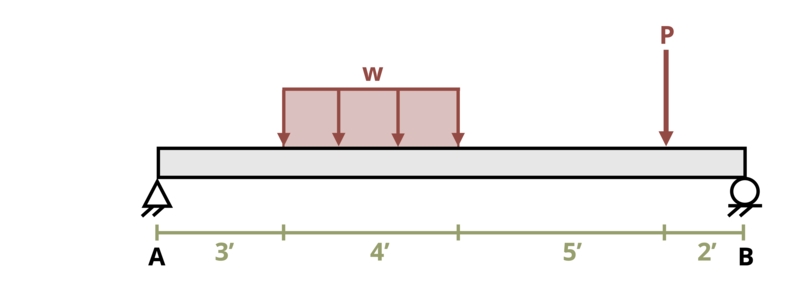
\includegraphics[keepaspectratio]{images/641.png}}
{[}Problem adapted from © Chris Galitz CC BY NC-SA 4.0{]}

\begin{Shaded}
\begin{Highlighting}[]
\NormalTok{\#| standalone: true}
\NormalTok{\#| viewerHeight: 600}
\NormalTok{\#| components: [viewer]}

\NormalTok{from shiny import App, render, ui, reactive}
\NormalTok{import random}
\NormalTok{import asyncio}
\NormalTok{import io}
\NormalTok{import math}
\NormalTok{import string}
\NormalTok{from datetime import datetime}
\NormalTok{from pathlib import Path}

\NormalTok{def generate\_random\_letters(length):}
\NormalTok{    \# Generate a random string of letters of specified length}
\NormalTok{    return "".join(random.choice(string.ascii\_lowercase) for \_ in range(length))}

\NormalTok{problem\_ID = "641"}
\NormalTok{P = reactive.Value("\_\_")}
\NormalTok{w = reactive.Value("\_\_")}
\NormalTok{attempts = ["Timestamp,Attempt,Answer1,Answer2,Feedback\textbackslash{}n"]}

\NormalTok{app\_ui = ui.page\_fluid(}
\NormalTok{    \#ui.markdown("**Please enter your ID number from your instructor and click to generate your problem**"),}
\NormalTok{    \#ui.input\_text("ID", "", placeholder="Enter ID Number Here"),}
\NormalTok{    \#ui.input\_action\_button("generate\_problem", "Generate Problem", class\_="btn{-}primary"),}
\NormalTok{    ui.markdown("**Problem Statement**"),}
\NormalTok{    ui.output\_ui("ui\_problem\_statement"),}
\NormalTok{    ui.input\_text("answer1", "Your Answer 1 in units of kip", placeholder="Please enter your answer 1"),}
\NormalTok{    ui.input\_text("answer2", "Your Answer 2 in units of kip", placeholder="Please enter your answer 2"),}
\NormalTok{    ui.input\_action\_button("submit", "Check Answers", class\_="btn{-}primary"),}
\NormalTok{    \#ui.download\_button("download", "Download File to Submit", class\_="btn{-}success"),}
\NormalTok{)}

\NormalTok{def server(input, output, session):}
\NormalTok{    \# Initialize a counter for attempts}
\NormalTok{    attempt\_counter = reactive.Value(0)}

\NormalTok{    @output}
\NormalTok{    @render.ui}
\NormalTok{    def ui\_problem\_statement():}
\NormalTok{        randomize\_vars()}
\NormalTok{        return [}
\NormalTok{            ui.markdown(}
\NormalTok{                f"The simply{-}supported beam is subjected to the loading shown. Determine the support reactions at A and B given P = \{P()\} kips and w = \{w()\} kip/ft."}
\NormalTok{            )}
\NormalTok{        ]}

\NormalTok{    \#@reactive.Effect}
\NormalTok{    \#@reactive.event(input.generate\_problem)}
\NormalTok{    def randomize\_vars():}
\NormalTok{        random.seed(101)}
\NormalTok{        P.set(random.randrange(5,50,1))}
\NormalTok{        w.set(random.randrange(20,100,1)/10)}
        
\NormalTok{    @reactive.Effect}
\NormalTok{    @reactive.event(input.submit)}
\NormalTok{    def \_():}
\NormalTok{        attempt\_counter.set(}
\NormalTok{            attempt\_counter() + 1}
\NormalTok{        )  \# Increment the attempt counter on each submission.}

\NormalTok{        \# Calculate the instructor\textquotesingle{}s answer and determine if the user\textquotesingle{}s answer is correct.}
\NormalTok{        instr1 = 4*w()+P(){-}(20*w()+12*P())/14}
\NormalTok{        instr2 = (20*w()+12*P())/14}

\NormalTok{        correct1 = math.isclose(float(input.answer1()), instr1, rel\_tol=0.01)}
\NormalTok{        correct2 = math.isclose(float(input.answer2()), instr2, rel\_tol=0.01)}
        
\NormalTok{        if correct1 and correct2:}
\NormalTok{            check = f"\{\textquotesingle{}both correct.\textquotesingle{}\}"}
\NormalTok{        elif correct1:}
\NormalTok{            check = f" \{\textquotesingle{}correct for answer 1 and incorrect for answer 2.\textquotesingle{}\}"}
\NormalTok{        elif correct2:}
\NormalTok{            check = f"\{\textquotesingle{}incorrect for answer 1 and correct for answer 2.\textquotesingle{}\}"}
\NormalTok{        else:}
\NormalTok{            check = f"\{\textquotesingle{}both incorrect.\textquotesingle{}\}"}
        
\NormalTok{        correct\_indicator = "JL" if correct1 and correct2 else "JG"}

\NormalTok{        random\_start = generate\_random\_letters(4)}
\NormalTok{        random\_middle = generate\_random\_letters(4)}
\NormalTok{        random\_end = generate\_random\_letters(4)}
\NormalTok{        \#encoded\_attempt = f"\{random\_start\}\{problem\_ID\}{-}\{random\_middle\}\{attempt\_counter()\}\{correct\_indicator\}{-}\{random\_end\}\{input.ID()\}"}

\NormalTok{        \#session.encoded\_attempt = reactive.Value(encoded\_attempt)}
\NormalTok{        attempts.append(f"\{datetime.now()\}, \{attempt\_counter()\}, \{input.answer1()\}, \{input.answer2()\}, \{check\}\textbackslash{}n")}

\NormalTok{        feedback = ui.markdown(f"Your answers of \{input.answer1()\} and \{input.answer2()\} are \{check\}.")}
\NormalTok{        m = ui.modal(feedback, title="Feedback", easy\_close=True)}
\NormalTok{        ui.modal\_show(m)}

\NormalTok{    \#@render.download(filename=lambda: f"Problem\_Log{-}\{problem\_ID\}{-}\{input.ID()\}.csv")}
\NormalTok{    async def download():}
\NormalTok{        final\_encoded = session.encoded\_attempt() if session.encoded\_attempt is not None else "No attempts"}
\NormalTok{        yield f"\{final\_encoded\}\textbackslash{}n\textbackslash{}n"}
\NormalTok{        yield "Timestamp,Attempt,Answer1,Answer2,Feedback\textbackslash{}n"}
\NormalTok{        for attempt in attempts[1:]:}
\NormalTok{            await asyncio.sleep(0.25)}
\NormalTok{            yield attempt}

\NormalTok{app = App(app\_ui, server)}
\end{Highlighting}
\end{Shaded}

\chapter*{Problem 1.2 - Equilibrium in
2D}\label{problem-1.2---equilibrium-in-2d}
\addcontentsline{toc}{chapter}{Problem 1.2 - Equilibrium in 2D}

\markboth{Problem 1.2 - Equilibrium in 2D}{Problem 1.2 - Equilibrium in
2D}

\pandocbounded{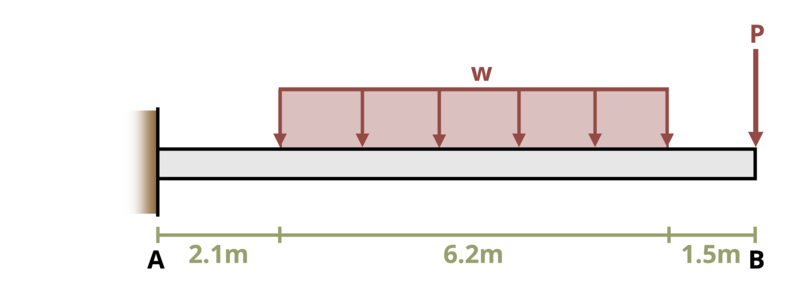
\includegraphics[keepaspectratio]{images/642.png}}
{[}Problem adapted from © Chris Galitz CC BY NC-SA 4.0{]}

\begin{Shaded}
\begin{Highlighting}[]
\NormalTok{\#| standalone: true}
\NormalTok{\#| viewerHeight: 600}
\NormalTok{\#| components: [viewer]}

\NormalTok{from shiny import App, render, ui, reactive}
\NormalTok{import random}
\NormalTok{import asyncio}
\NormalTok{import io}
\NormalTok{import math}
\NormalTok{import string}
\NormalTok{from datetime import datetime}
\NormalTok{from pathlib import Path}

\NormalTok{def generate\_random\_letters(length):}
\NormalTok{    \# Generate a random string of letters of specified length}
\NormalTok{    return "".join(random.choice(string.ascii\_lowercase) for \_ in range(length))}

\NormalTok{problem\_ID = "642"}
\NormalTok{P = reactive.Value("\_\_")}
\NormalTok{w = reactive.Value("\_\_")}
\NormalTok{attempts = ["Timestamp,Attempt,Answer1,Answer2,Feedback\textbackslash{}n"]}

\NormalTok{app\_ui = ui.page\_fluid(}
\NormalTok{    \#ui.markdown("**Please enter your ID number from your instructor and click to generate your problem**"),}
\NormalTok{    \#ui.input\_text("ID", "", placeholder="Enter ID Number Here"),}
\NormalTok{    \#ui.input\_action\_button("generate\_problem", "Generate Problem", class\_="btn{-}primary"),}
\NormalTok{    ui.markdown("**Problem Statement**"),}
\NormalTok{    ui.output\_ui("ui\_problem\_statement"),}
\NormalTok{    ui.input\_text("answer1", "Your Answer 1 in units of kN", placeholder="Please enter your answer 1"),}
\NormalTok{    ui.input\_text("answer2", "Your Answer 2 in units of kN{-}m", placeholder="Please enter your answer 2"),}
\NormalTok{    ui.input\_action\_button("submit", "Check Answers", class\_="btn{-}primary"),}
\NormalTok{    \#ui.download\_button("download", "Download File to Submit", class\_="btn{-}success"),}
\NormalTok{)}

\NormalTok{def server(input, output, session):}
\NormalTok{    \# Initialize a counter for attempts}
\NormalTok{    attempt\_counter = reactive.Value(0)}

\NormalTok{    @output}
\NormalTok{    @render.ui}
\NormalTok{    def ui\_problem\_statement():}
\NormalTok{        randomize\_vars()}
\NormalTok{        return [}
\NormalTok{            ui.markdown(}
\NormalTok{                f"The cantilever beam is subjected to the loading shown. Determine the reactions at A given P = \{P()\} kN and w = \{w()\} kN/m."}
\NormalTok{            )}
\NormalTok{        ]}

\NormalTok{    \#@reactive.Effect}
\NormalTok{    \#@reactive.event(input.generate\_problem)}
\NormalTok{    def randomize\_vars():}
\NormalTok{        random.seed(101)}
\NormalTok{        P.set(random.randrange(5,30,1))}
\NormalTok{        w.set(random.randrange(20,50,1)/10)}
        
\NormalTok{    @reactive.Effect}
\NormalTok{    @reactive.event(input.submit)}
\NormalTok{    def \_():}
\NormalTok{        attempt\_counter.set(}
\NormalTok{            attempt\_counter() + 1}
\NormalTok{        )  \# Increment the attempt counter on each submission.}

\NormalTok{        \# Calculate the instructor\textquotesingle{}s answer and determine if the user\textquotesingle{}s answer is correct.}
\NormalTok{        instr1 = P()+w()*6.2}
\NormalTok{        instr2 = P()*(2.1+6.2+1.5)+w()*6.2*5.2}

\NormalTok{        correct1 = math.isclose(float(input.answer1()), instr1, rel\_tol=0.01)}
\NormalTok{        correct2 = math.isclose(float(input.answer2()), instr2, rel\_tol=0.01)}
        
\NormalTok{        if correct1 and correct2:}
\NormalTok{            check = f"\{\textquotesingle{}both correct.\textquotesingle{}\}"}
\NormalTok{        elif correct1:}
\NormalTok{            check = f" \{\textquotesingle{}correct for answer 1 and incorrect for answer 2.\textquotesingle{}\}"}
\NormalTok{        elif correct2:}
\NormalTok{            check = f"\{\textquotesingle{}incorrect for answer 1 and correct for answer 2.\textquotesingle{}\}"}
\NormalTok{        else:}
\NormalTok{            check = f"\{\textquotesingle{}both incorrect.\textquotesingle{}\}"}
        
\NormalTok{        correct\_indicator = "JL" if correct1 and correct2 else "JG"}

\NormalTok{        random\_start = generate\_random\_letters(4)}
\NormalTok{        random\_middle = generate\_random\_letters(4)}
\NormalTok{        random\_end = generate\_random\_letters(4)}
\NormalTok{        \#encoded\_attempt = f"\{random\_start\}\{problem\_ID\}{-}\{random\_middle\}\{attempt\_counter()\}\{correct\_indicator\}{-}\{random\_end\}\{input.ID()\}"}

\NormalTok{        \#session.encoded\_attempt = reactive.Value(encoded\_attempt)}
\NormalTok{        attempts.append(f"\{datetime.now()\}, \{attempt\_counter()\}, \{input.answer1()\}, \{input.answer2()\}, \{check\}\textbackslash{}n")}

\NormalTok{        feedback = ui.markdown(f"Your answers of \{input.answer1()\} and \{input.answer2()\} are \{check\}.")}
\NormalTok{        m = ui.modal(feedback, title="Feedback", easy\_close=True)}
\NormalTok{        ui.modal\_show(m)}

\NormalTok{    \#@render.download(filename=lambda: f"Problem\_Log{-}\{problem\_ID\}{-}\{input.ID()\}.csv")}
\NormalTok{    async def download():}
\NormalTok{        final\_encoded = session.encoded\_attempt() if session.encoded\_attempt is not None else "No attempts"}
\NormalTok{        yield f"\{final\_encoded\}\textbackslash{}n\textbackslash{}n"}
\NormalTok{        yield "Timestamp,Attempt,Answer1,Answer2,Feedback\textbackslash{}n"}
\NormalTok{        for attempt in attempts[1:]:}
\NormalTok{            await asyncio.sleep(0.25)}
\NormalTok{            yield attempt}

\NormalTok{app = App(app\_ui, server)}
\end{Highlighting}
\end{Shaded}

\chapter*{Problem 1.3 - Equilibrium in
2D}\label{problem-1.3---equilibrium-in-2d}
\addcontentsline{toc}{chapter}{Problem 1.3 - Equilibrium in 2D}

\markboth{Problem 1.3 - Equilibrium in 2D}{Problem 1.3 - Equilibrium in
2D}

\pandocbounded{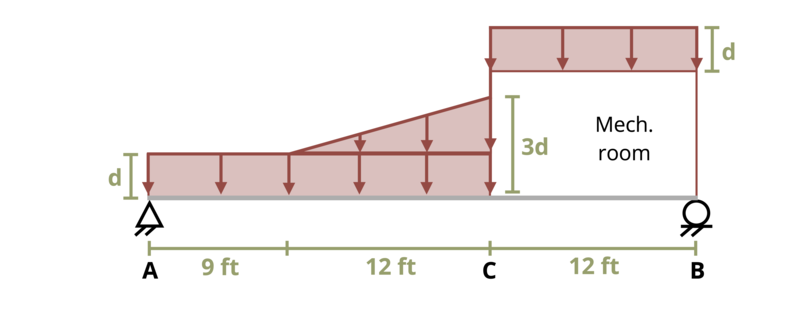
\includegraphics[keepaspectratio]{images/643.png}}
{[}Problem adapted from © Chris Galitz CC BY NC-SA 4.0{]}

\begin{Shaded}
\begin{Highlighting}[]
\NormalTok{\#| standalone: true}
\NormalTok{\#| viewerHeight: 600}
\NormalTok{\#| components: [viewer]}

\NormalTok{from shiny import App, render, ui, reactive}
\NormalTok{import random}
\NormalTok{import asyncio}
\NormalTok{import io}
\NormalTok{import math}
\NormalTok{import string}
\NormalTok{from datetime import datetime}
\NormalTok{from pathlib import Path}

\NormalTok{def generate\_random\_letters(length):}
\NormalTok{    \# Generate a random string of letters of specified length}
\NormalTok{    return "".join(random.choice(string.ascii\_lowercase) for \_ in range(length))}

\NormalTok{problem\_ID = "643"}
\NormalTok{d = reactive.Value("\_\_")}
\NormalTok{w = reactive.Value("\_\_")}
\NormalTok{attempts = ["Timestamp,Attempt,Answer1,Answer2,Feedback\textbackslash{}n"]}

\NormalTok{app\_ui = ui.page\_fluid(}
\NormalTok{    \#ui.markdown("**Please enter your ID number from your instructor and click to generate your problem**"),}
\NormalTok{    \#ui.input\_text("ID", "", placeholder="Enter ID Number Here"),}
\NormalTok{    \#ui.input\_action\_button("generate\_problem", "Generate Problem", class\_="btn{-}primary"),}
\NormalTok{    ui.markdown("**Problem Statement**"),}
\NormalTok{    ui.output\_ui("ui\_problem\_statement"),}
\NormalTok{    ui.input\_text("answer1", "Your Answer 1 in units of kip", placeholder="Please enter your answer 1"),}
\NormalTok{    ui.input\_text("answer2", "Your Answer 2 in units of kip", placeholder="Please enter your answer 2"),}
\NormalTok{    ui.input\_action\_button("submit", "Check Answers", class\_="btn{-}primary"),}
\NormalTok{    \#ui.download\_button("download", "Download File to Submit", class\_="btn{-}success"),}
\NormalTok{)}

\NormalTok{def server(input, output, session):}
\NormalTok{    \# Initialize a counter for attempts}
\NormalTok{    attempt\_counter = reactive.Value(0)}

\NormalTok{    @output}
\NormalTok{    @render.ui}
\NormalTok{    def ui\_problem\_statement():}
\NormalTok{        randomize\_vars()}
\NormalTok{        return [}
\NormalTok{            ui.markdown(}
\NormalTok{                f"The simply{-}supported roof beam AB is subjected to snow loads as a uniform load with snow depth d = \{d()\} in. A mechanical room on the roof is also covered by snow, and transmits half of the the snow load between points B and C to the roof at point B and the other half at point C. Additionally, there is a snow drift as shown with maximum height, 3*d, above the roof. If the distributed weight of snow is W = \{w()\} lb/ft per inch of thickness, determine the reactions at supports A and B."}
\NormalTok{            )}
\NormalTok{        ]}

\NormalTok{    \#@reactive.Effect}
\NormalTok{    \#@reactive.event(input.generate\_problem)}
\NormalTok{    def randomize\_vars():}
\NormalTok{        random.seed(101)}
\NormalTok{        d.set(random.randrange(10,30,1))}
\NormalTok{        w.set(random.randrange(40,80,1))}
        
\NormalTok{    @reactive.Effect}
\NormalTok{    @reactive.event(input.submit)}
\NormalTok{    def \_():}
\NormalTok{        attempt\_counter.set(}
\NormalTok{            attempt\_counter() + 1}
\NormalTok{        )  \# Increment the attempt counter on each submission.}

\NormalTok{        \# Calculate the instructor\textquotesingle{}s answer and determine if the user\textquotesingle{}s answer is correct.}
\NormalTok{        w1 = w()*12*d()}
\NormalTok{        w2 = w()*21*d()}
\NormalTok{        w3 = 0.5*w()*2*d()*12}
\NormalTok{        instr1 = (w1+w2+w3{-}(10.5*w2+17*w3+21*w1/2+33*w1/2)/33)/1000}
\NormalTok{        instr2 = ((10.5*w2+17*w3+21*w1/2+33*w1/2)/33)/1000}

\NormalTok{        correct1 = math.isclose(float(input.answer1()), instr1, rel\_tol=0.01)}
\NormalTok{        correct2 = math.isclose(float(input.answer2()), instr2, rel\_tol=0.01)}
        
\NormalTok{        if correct1 and correct2:}
\NormalTok{            check = f"\{\textquotesingle{}both correct.\textquotesingle{}\}"}
\NormalTok{        elif correct1:}
\NormalTok{            check = f" \{\textquotesingle{}correct for answer 1 and incorrect for answer 2.\textquotesingle{}\}"}
\NormalTok{        elif correct2:}
\NormalTok{            check = f"\{\textquotesingle{}incorrect for answer 1 and correct for answer 2.\textquotesingle{}\}"}
\NormalTok{        else:}
\NormalTok{            check = f"\{\textquotesingle{}both incorrect.\textquotesingle{}\}"}
        
\NormalTok{        correct\_indicator = "JL" if correct1 and correct2 else "JG"}

\NormalTok{        random\_start = generate\_random\_letters(4)}
\NormalTok{        random\_middle = generate\_random\_letters(4)}
\NormalTok{        random\_end = generate\_random\_letters(4)}
\NormalTok{        \#encoded\_attempt = f"\{random\_start\}\{problem\_ID\}{-}\{random\_middle\}\{attempt\_counter()\}\{correct\_indicator\}{-}\{random\_end\}\{input.ID()\}"}

\NormalTok{        \#session.encoded\_attempt = reactive.Value(encoded\_attempt)}
\NormalTok{        attempts.append(f"\{datetime.now()\}, \{attempt\_counter()\}, \{input.answer1()\}, \{input.answer2()\}, \{check\}\textbackslash{}n")}

\NormalTok{        feedback = ui.markdown(f"Your answers of \{input.answer1()\} and \{input.answer2()\} are \{check\}.")}
\NormalTok{        m = ui.modal(feedback, title="Feedback", easy\_close=True)}
\NormalTok{        ui.modal\_show(m)}

\NormalTok{    \#@render.download(filename=lambda: f"Problem\_Log{-}\{problem\_ID\}{-}\{input.ID()\}.csv")}
\NormalTok{    async def download():}
\NormalTok{        final\_encoded = session.encoded\_attempt() if session.encoded\_attempt is not None else "No attempts"}
\NormalTok{        yield f"\{final\_encoded\}\textbackslash{}n\textbackslash{}n"}
\NormalTok{        yield "Timestamp,Attempt,Answer1,Answer2,Feedback\textbackslash{}n"}
\NormalTok{        for attempt in attempts[1:]:}
\NormalTok{            await asyncio.sleep(0.25)}
\NormalTok{            yield attempt}

\NormalTok{app = App(app\_ui, server)}
\end{Highlighting}
\end{Shaded}

\chapter*{Problem 1.4 - Internal
Reactions}\label{problem-1.4---internal-reactions}
\addcontentsline{toc}{chapter}{Problem 1.4 - Internal Reactions}

\markboth{Problem 1.4 - Internal Reactions}{Problem 1.4 - Internal
Reactions}

\pandocbounded{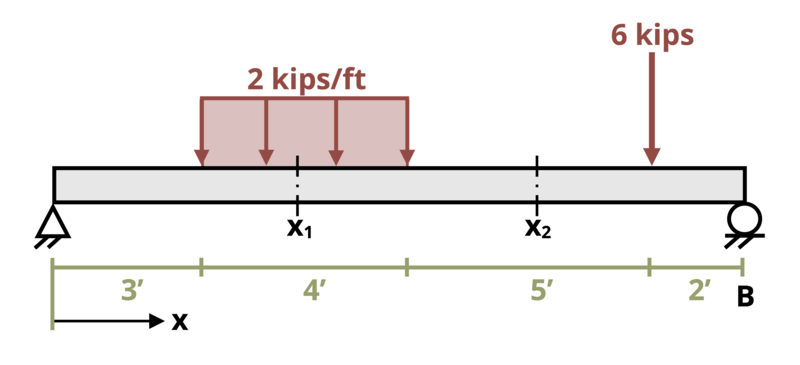
\includegraphics[keepaspectratio]{images/644.png}}
{[}Problem adapted from © Chris Galitz CC BY NC-SA 4.0{]}

\begin{Shaded}
\begin{Highlighting}[]
\NormalTok{\#| standalone: true}
\NormalTok{\#| viewerHeight: 600}
\NormalTok{\#| components: [viewer]}

\NormalTok{from shiny import App, render, ui, reactive}
\NormalTok{import random}
\NormalTok{import asyncio}
\NormalTok{import io}
\NormalTok{import math}
\NormalTok{import string}
\NormalTok{from datetime import datetime}
\NormalTok{from pathlib import Path}

\NormalTok{def generate\_random\_letters(length):}
\NormalTok{    \# Generate a random string of letters of specified length}
\NormalTok{    return "".join(random.choice(string.ascii\_lowercase) for \_ in range(length))}

\NormalTok{problem\_ID = "644"}
\NormalTok{x1 = reactive.Value("\_\_")}
\NormalTok{x2 = reactive.Value("\_\_")}
\NormalTok{P = reactive.Value("\_\_")}
\NormalTok{w = reactive.Value("\_\_")}
\NormalTok{attempts = ["Timestamp,Attempt,Answer1,Answer2,Answer3,Answer4,Answer5,Answer6,Feedback\textbackslash{}n"]}

\NormalTok{app\_ui = ui.page\_fluid(}
\NormalTok{    \#ui.markdown("**Please enter your ID number from your instructor and click to generate your problem**"),}
\NormalTok{    \#ui.input\_text("ID", "", placeholder="Enter ID Number Here"),}
\NormalTok{    \#ui.input\_action\_button("generate\_problem", "Generate Problem", class\_="btn{-}primary"),}
\NormalTok{    ui.markdown("**Problem Statement**"),}
\NormalTok{    ui.output\_ui("ui\_problem\_statement"),}
\NormalTok{    ui.input\_text("answer1", "Your Answer 1 in units of kip", placeholder="Please enter your answer 1"),}
\NormalTok{    ui.input\_text("answer2", "Your Answer 2 in units of kip", placeholder="Please enter your answer 2"),}
\NormalTok{    ui.input\_text("answer3", "Your Answer 3 in units of kip{-}ft", placeholder="Please enter your answer 2"),}
\NormalTok{    ui.input\_text("answer4", "Your Answer 4 in units of kip", placeholder="Please enter your answer 2"),}
\NormalTok{    ui.input\_text("answer5", "Your Answer 5 in units of kip", placeholder="Please enter your answer 2"),}
\NormalTok{    ui.input\_text("answer6", "Your Answer 6 in units of kip{-}ft", placeholder="Please enter your answer 2"),}

\NormalTok{    ui.input\_action\_button("submit", "Check Answers", class\_="btn{-}primary"),}
\NormalTok{    \#ui.download\_button("download", "Download File to Submit", class\_="btn{-}success"),}
\NormalTok{)}

\NormalTok{def server(input, output, session):}
\NormalTok{    \# Initialize a counter for attempts}
\NormalTok{    attempt\_counter = reactive.Value(0)}

\NormalTok{    @output}
\NormalTok{    @render.ui}
\NormalTok{    def ui\_problem\_statement():}
\NormalTok{        randomize\_vars()}
\NormalTok{        return [}
\NormalTok{            ui.markdown(}
\NormalTok{                f"The simply{-}supported beam is subjected to the loading shown. Determine the internal normal force, N, shear force, V, and bending moment, M, at locations x\textless{}sub\textgreater{}1\textless{}/sub\textgreater{} = \{x1()\} ft and x\textless{}sub\textgreater{}2\textless{}/sub\textgreater{} = \{x2()\} ft. Assume loads P = \{P()\} kips and w = \{w()\} kips/ft. Use appropriate signs in your answers."}
\NormalTok{            )}
\NormalTok{        ]}

\NormalTok{    \#@reactive.Effect}
\NormalTok{    \#@reactive.event(input.generate\_problem)}
\NormalTok{    def randomize\_vars():}
\NormalTok{        random.seed(101)}
\NormalTok{        x1.set(random.randrange(41,69,1)/10)}
\NormalTok{        x2.set(random.randrange(75,115,1)/10)}
\NormalTok{        P.set(6) \#random.randrange(5,25,1))}
\NormalTok{        w.set(2) \#random.randrange(20,50,1)/10)}
        
\NormalTok{    @reactive.Effect}
\NormalTok{    @reactive.event(input.submit)}
\NormalTok{    def \_():}
\NormalTok{        attempt\_counter.set(}
\NormalTok{            attempt\_counter() + 1}
\NormalTok{        )  \# Increment the attempt counter on each submission.}

\NormalTok{        \# Calculate the instructor\textquotesingle{}s answer and determine if the user\textquotesingle{}s answer is correct.}
\NormalTok{        instr1 = 0}
\NormalTok{        Ay = (P()*2+w()*4*9)/14}
\NormalTok{        instr2 = Ay{-}w()*(x1(){-}3)}
\NormalTok{        instr3 = w()*(x1(){-}3)*(3+(x1(){-}3)/2)+instr2*x1()}
\NormalTok{        instr4=0}
\NormalTok{        instr5= Ay{-}w()*4}
\NormalTok{        instr6= w()*4*5+instr5*x2()}

\NormalTok{        correct1 = math.isclose(float(input.answer1()), instr1, rel\_tol=0.01)}
\NormalTok{        correct2 = math.isclose(float(input.answer2()), instr2, rel\_tol=0.01)}
\NormalTok{        correct3 = math.isclose(float(input.answer3()), instr3, rel\_tol=0.01)}
\NormalTok{        correct4 = math.isclose(float(input.answer4()), instr4, rel\_tol=0.01)}
\NormalTok{        correct5 = math.isclose(float(input.answer5()), instr5, rel\_tol=0.01)}
\NormalTok{        correct6 = math.isclose(float(input.answer6()), instr6, rel\_tol=0.01)}

\NormalTok{        if correct1 and correct2 and correct3 and correct4 and correct5 and correct6:}
\NormalTok{            check = "All answers are correct."}
\NormalTok{        else:}
\NormalTok{            conditions = []}
\NormalTok{            for i, correct in enumerate([correct1, correct2, correct3, correct4, correct5, correct6], start=1):}
\NormalTok{                if correct:}
\NormalTok{                    conditions.append(f"correct for answer \{i\}")}
\NormalTok{                else:}
\NormalTok{                    conditions.append(f"incorrect for answer \{i\}")}
\NormalTok{            check = "; ".join(conditions) + "."}
        
\NormalTok{        correct\_indicator = "JL" if correct1 and correct2 and correct3 and correct4 and correct5 and correct6 else "JG"}

\NormalTok{        random\_start = generate\_random\_letters(4)}
\NormalTok{        random\_middle = generate\_random\_letters(4)}
\NormalTok{        random\_end = generate\_random\_letters(4)}
\NormalTok{        \#encoded\_attempt = f"\{random\_start\}\{problem\_ID\}{-}\{random\_middle\}\{attempt\_counter()\}\{correct\_indicator\}{-}\{random\_end\}\{input.ID()\}"}

\NormalTok{        \#session.encoded\_attempt = reactive.Value(encoded\_attempt)}
\NormalTok{        attempts.append(f"\{datetime.now()\}, \{attempt\_counter()\}, \{input.answer1()\}, \{input.answer2()\}, \{check\}\textbackslash{}n")}

\NormalTok{        feedback = ui.markdown(f"Your answers of \{input.answer1()\}, \{input.answer2()\}, \{input.answer3()\}, \{input.answer4()\}, \{input.answer5()\}, and \{input.answer6()\}  are \{check\}.")}
\NormalTok{        m = ui.modal(feedback, title="Feedback", easy\_close=True)}
\NormalTok{        ui.modal\_show(m)}

\NormalTok{    \#@render.download(filename=lambda: f"Problem\_Log{-}\{problem\_ID\}{-}\{input.ID()\}.csv")}
\NormalTok{    async def download():}
\NormalTok{        final\_encoded = session.encoded\_attempt() if session.encoded\_attempt is not None else "No attempts"}
\NormalTok{        yield f"\{final\_encoded\}\textbackslash{}n\textbackslash{}n"}
\NormalTok{        yield "Timestamp,Attempt,Answer1,Answer2,Feedback\textbackslash{}n"}
\NormalTok{        for attempt in attempts[1:]:}
\NormalTok{            await asyncio.sleep(0.25)}
\NormalTok{            yield attempt}

\NormalTok{app = App(app\_ui, server)}
\end{Highlighting}
\end{Shaded}

\chapter*{Problem 1.5 - Internal
Reactions}\label{problem-1.5---internal-reactions}
\addcontentsline{toc}{chapter}{Problem 1.5 - Internal Reactions}

\markboth{Problem 1.5 - Internal Reactions}{Problem 1.5 - Internal
Reactions}

\pandocbounded{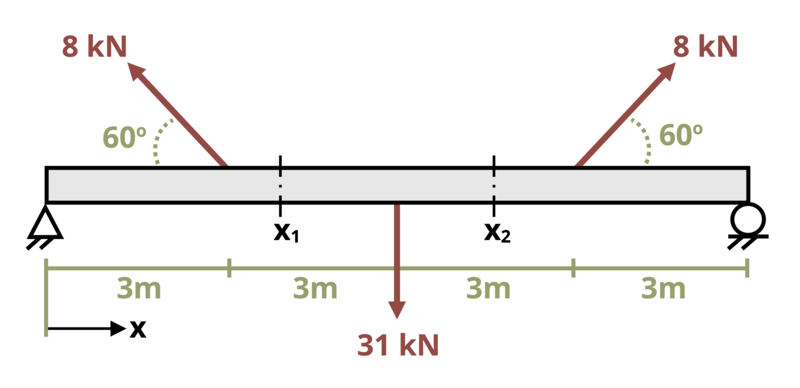
\includegraphics[keepaspectratio]{images/645.png}}
{[}Problem adapted from © Chris Galitz CC BY NC-SA 4.0{]}

\begin{Shaded}
\begin{Highlighting}[]
\NormalTok{\#| standalone: true}
\NormalTok{\#| viewerHeight: 600}
\NormalTok{\#| components: [viewer]}

\NormalTok{from shiny import App, render, ui, reactive}
\NormalTok{import random}
\NormalTok{import asyncio}
\NormalTok{import io}
\NormalTok{import math}
\NormalTok{import string}
\NormalTok{from datetime import datetime}
\NormalTok{from pathlib import Path}

\NormalTok{def generate\_random\_letters(length):}
\NormalTok{    \# Generate a random string of letters of specified length}
\NormalTok{    return "".join(random.choice(string.ascii\_lowercase) for \_ in range(length))}

\NormalTok{problem\_ID = "645"}
\NormalTok{x = reactive.Value("\_\_")}
\NormalTok{F1 = reactive.Value("\_\_")}
\NormalTok{F2 = reactive.Value("\_\_")}
\NormalTok{F3 = reactive.Value("\_\_")}
\NormalTok{attempts = ["Timestamp,Attempt,Answer1,Answer2,Answer3,Feedback\textbackslash{}n"]}

\NormalTok{app\_ui = ui.page\_fluid(}
\NormalTok{    \#ui.markdown("**Please enter your ID number from your instructor and click to generate your problem**"),}
\NormalTok{    \#ui.input\_text("ID", "", placeholder="Enter ID Number Here"),}
\NormalTok{    \#ui.input\_action\_button("generate\_problem", "Generate Problem", class\_="btn{-}primary"),}
\NormalTok{    ui.markdown("**Problem Statement**"),}
\NormalTok{    ui.output\_ui("ui\_problem\_statement"),}
\NormalTok{    ui.input\_text("answer1", "Your Answer 1 in units of kN", placeholder="Please enter your answer 1"),}
\NormalTok{    ui.input\_text("answer2", "Your Answer 2 in units of kN", placeholder="Please enter your answer 2"),}
\NormalTok{    ui.input\_text("answer3", "Your Answer 3 in units of kN{-}m", placeholder="Please enter your answer 2"),}

\NormalTok{    ui.input\_action\_button("submit", "Check Answers", class\_="btn{-}primary"),}
\NormalTok{    \#ui.download\_button("download", "Download File to Submit", class\_="btn{-}success"),}
\NormalTok{)}

\NormalTok{def server(input, output, session):}
\NormalTok{    \# Initialize a counter for attempts}
\NormalTok{    attempt\_counter = reactive.Value(0)}

\NormalTok{    @output}
\NormalTok{    @render.ui}
\NormalTok{    def ui\_problem\_statement():}
\NormalTok{        randomize\_vars()}
\NormalTok{        return [}
\NormalTok{            ui.markdown(}
\NormalTok{                f"The simply{-}supported beam is subjected to the loading shown. Determine the internal normal force, N, shear force, V, and bending moment, M, at x\textless{}sub\textgreater{}2\textless{}/sub\textgreater{} = \{x()\} m (ignore the cut at x\textless{}sub\textgreater{}1\textless{}/sub\textgreater{} for this problem). Assume forces F\textless{}sub\textgreater{}1\textless{}/sub\textgreater{} = \{F1()\} kN, F\textless{}sub\textgreater{}2\textless{}/sub\textgreater{} = \{F2()\} kN, and F\textless{}sub\textgreater{}3\textless{}/sub\textgreater{} = \{F3()\} kN. Use appropriate signs in your answers."}
\NormalTok{            )}
\NormalTok{        ]}

\NormalTok{    \#@reactive.Effect}
\NormalTok{    \#@reactive.event(input.generate\_problem)}
\NormalTok{    def randomize\_vars():}
\NormalTok{        random.seed(101)}
\NormalTok{        x.set(6.8) \#random.randrange(61,89,1)/10)}
\NormalTok{        F1.set(8) \#random.randrange(5,15,1))}
\NormalTok{        F2.set(31) \#random.randrange(20,40,1))}
\NormalTok{        F3.set(8) \#random.randrange(5,15,1))}
        
\NormalTok{    @reactive.Effect}
\NormalTok{    @reactive.event(input.submit)}
\NormalTok{    def \_():}
\NormalTok{        attempt\_counter.set(}
\NormalTok{            attempt\_counter() + 1}
\NormalTok{        )  \# Increment the attempt counter on each submission.}

\NormalTok{        \# Calculate the instructor\textquotesingle{}s answer and determine if the user\textquotesingle{}s answer is correct.}
\NormalTok{        Ax = F1()*math.cos(math.pi/3){-}F3()*math.cos(math.pi/3)}
\NormalTok{        Ay = ({-}F1()*math.sin(math.pi/3)*9{-}F3()*math.sin(math.pi/3)*3+F2()*6)/12}
\NormalTok{        instr1 = F1()*math.cos(math.pi/3)}
\NormalTok{        instr2 = Ay+F1()*math.sin(math.pi/3){-}31}
\NormalTok{        instr3 = {-}F1()*math.sin(math.pi/3)*3+instr2*x()+31*6}

\NormalTok{        correct1 = math.isclose(float(input.answer1()), instr1, rel\_tol=0.01)}
\NormalTok{        correct2 = math.isclose(float(input.answer2()), instr2, rel\_tol=0.01)}
\NormalTok{        correct3 = math.isclose(float(input.answer3()), instr3, rel\_tol=0.01)}

\NormalTok{        if correct1 and correct2 and correct3:}
\NormalTok{            check = "All answers are correct."}
\NormalTok{        else:}
\NormalTok{            conditions = []}
\NormalTok{            for i, correct in enumerate([correct1, correct2, correct3], start=1):}
\NormalTok{                if correct:}
\NormalTok{                    conditions.append(f"correct for answer \{i\}")}
\NormalTok{                else:}
\NormalTok{                    conditions.append(f"incorrect for answer \{i\}")}
\NormalTok{            check = "; ".join(conditions) + "."}
        
\NormalTok{        correct\_indicator = "JL" if correct1 and correct2 and correct3 else "JG"}

\NormalTok{        random\_start = generate\_random\_letters(4)}
\NormalTok{        random\_middle = generate\_random\_letters(4)}
\NormalTok{        random\_end = generate\_random\_letters(4)}
\NormalTok{        \#encoded\_attempt = f"\{random\_start\}\{problem\_ID\}{-}\{random\_middle\}\{attempt\_counter()\}\{correct\_indicator\}{-}\{random\_end\}\{input.ID()\}"}

\NormalTok{        \#session.encoded\_attempt = reactive.Value(encoded\_attempt)}
\NormalTok{        attempts.append(f"\{datetime.now()\}, \{attempt\_counter()\}, \{input.answer1()\}, \{input.answer2()\}, \{check\}\textbackslash{}n")}

\NormalTok{        feedback = ui.markdown(f"Your answers of \{input.answer1()\}, \{input.answer2()\}, and \{input.answer3()\} are \{check\}.")}
\NormalTok{        m = ui.modal(feedback, title="Feedback", easy\_close=True)}
\NormalTok{        ui.modal\_show(m)}

\NormalTok{    \#@render.download(filename=lambda: f"Problem\_Log{-}\{problem\_ID\}{-}\{input.ID()\}.csv")}
\NormalTok{    async def download():}
\NormalTok{        final\_encoded = session.encoded\_attempt() if session.encoded\_attempt is not None else "No attempts"}
\NormalTok{        yield f"\{final\_encoded\}\textbackslash{}n\textbackslash{}n"}
\NormalTok{        yield "Timestamp,Attempt,Answer1,Answer2,Feedback\textbackslash{}n"}
\NormalTok{        for attempt in attempts[1:]:}
\NormalTok{            await asyncio.sleep(0.25)}
\NormalTok{            yield attempt}

\NormalTok{app = App(app\_ui, server)}
\end{Highlighting}
\end{Shaded}

\chapter*{Problem 1.6 - Internal
Reactions}\label{problem-1.6---internal-reactions}
\addcontentsline{toc}{chapter}{Problem 1.6 - Internal Reactions}

\markboth{Problem 1.6 - Internal Reactions}{Problem 1.6 - Internal
Reactions}

\pandocbounded{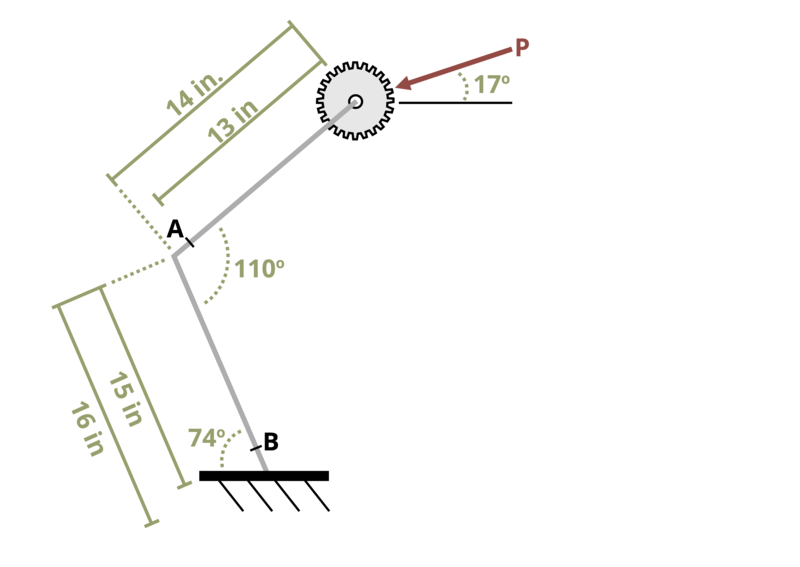
\includegraphics[keepaspectratio]{images/646.png}}
{[}Problem adapted from © Chris Galitz CC BY NC-SA 4.0{]}

\begin{Shaded}
\begin{Highlighting}[]
\NormalTok{\#| standalone: true}
\NormalTok{\#| viewerHeight: 600}
\NormalTok{\#| components: [viewer]}

\NormalTok{from shiny import App, render, ui, reactive}
\NormalTok{import random}
\NormalTok{import asyncio}
\NormalTok{import io}
\NormalTok{import math}
\NormalTok{import string}
\NormalTok{from datetime import datetime}
\NormalTok{from pathlib import Path}

\NormalTok{def generate\_random\_letters(length):}
\NormalTok{    \# Generate a random string of letters of specified length}
\NormalTok{    return "".join(random.choice(string.ascii\_lowercase) for \_ in range(length))}

\NormalTok{problem\_ID = "646"}
\NormalTok{P = reactive.Value("\_\_")}
\NormalTok{theta = reactive.Value("\_\_")}
\NormalTok{attempts = ["Timestamp,Attempt,Answer1,Answer2,Answer3,Feedback\textbackslash{}n"]}

\NormalTok{app\_ui = ui.page\_fluid(}
\NormalTok{    \#ui.markdown("**Please enter your ID number from your instructor and click to generate your problem**"),}
\NormalTok{    \#ui.input\_text("ID", "", placeholder="Enter ID Number Here"),}
\NormalTok{    \#ui.input\_action\_button("generate\_problem", "Generate Problem", class\_="btn{-}primary"),}
\NormalTok{    ui.markdown("**Problem Statement**"),}
\NormalTok{    ui.output\_ui("ui\_problem\_statement"),}
\NormalTok{    ui.input\_text("answer1", "Your Answer 1 in units of lb", placeholder="Please enter your answer 1"),}
\NormalTok{    ui.input\_text("answer2", "Your Answer 2 in units of lb", placeholder="Please enter your answer 2"),}
\NormalTok{    ui.input\_text("answer3", "Your Answer 3 in units of lb{-}in", placeholder="Please enter your answer 2"),}

\NormalTok{    ui.input\_action\_button("submit", "Check Answers", class\_="btn{-}primary"),}
\NormalTok{    \#ui.download\_button("download", "Download File to Submit", class\_="btn{-}success"),}
\NormalTok{)}

\NormalTok{def server(input, output, session):}
\NormalTok{    \# Initialize a counter for attempts}
\NormalTok{    attempt\_counter = reactive.Value(0)}

\NormalTok{    @output}
\NormalTok{    @render.ui}
\NormalTok{    def ui\_problem\_statement():}
\NormalTok{        randomize\_vars()}
\NormalTok{        return [}
\NormalTok{            ui.markdown(}
\NormalTok{                f"A gear shift, once engaged, can be modeled as the bent cantilever beam shown. If a force, P = \{P()\} lb at angle Θ = \{theta()\}, was used to engage the shifter, determine the magnitude of the internal normal force, N, shear force, V, and bending moment, M, at point B."}
\NormalTok{            )}
\NormalTok{        ]}

\NormalTok{    \#@reactive.Effect}
\NormalTok{    \#@reactive.event(input.generate\_problem)}
\NormalTok{    def randomize\_vars():}
\NormalTok{        random.seed(101)}
\NormalTok{        P.set(random.randrange(20,75,1))}
\NormalTok{        theta.set(random.randrange(10,25,1))}

\NormalTok{    @reactive.Effect}
\NormalTok{    @reactive.event(input.submit)}
\NormalTok{    def \_():}
\NormalTok{        attempt\_counter.set(}
\NormalTok{            attempt\_counter() + 1}
\NormalTok{        )  \# Increment the attempt counter on each submission.}

\NormalTok{        \# Calculate the instructor\textquotesingle{}s answer and determine if the user\textquotesingle{}s answer is correct.}
\NormalTok{        instr1 = abs(P()*math.cos((70+theta())*math.pi/180))}
\NormalTok{        instr2 = abs(P()*math.sin((70+theta())*math.pi/180))}
\NormalTok{        instr3 = abs(P()*math.sin((70+theta())*math.pi/180)*(15+14*math.cos(70*math.pi/180)){-}P()*math.cos((70+theta())*math.pi/180)*14*math.sin(70*math.pi/180))}

\NormalTok{        correct1 = math.isclose(float(input.answer1()), instr1, rel\_tol=0.01)}
\NormalTok{        correct2 = math.isclose(float(input.answer2()), instr2, rel\_tol=0.01)}
\NormalTok{        correct3 = math.isclose(float(input.answer3()), instr3, rel\_tol=0.01)}

\NormalTok{        if correct1 and correct2 and correct3:}
\NormalTok{            check = "All answers are correct."}
\NormalTok{        else:}
\NormalTok{            conditions = []}
\NormalTok{            for i, correct in enumerate([correct1, correct2, correct3], start=1):}
\NormalTok{                if correct:}
\NormalTok{                    conditions.append(f"correct for answer \{i\}")}
\NormalTok{                else:}
\NormalTok{                    conditions.append(f"incorrect for answer \{i\}")}
\NormalTok{            check = "; ".join(conditions) + "."}
        
\NormalTok{        correct\_indicator = "JL" if correct1 and correct2 and correct3 else "JG"}

\NormalTok{        random\_start = generate\_random\_letters(4)}
\NormalTok{        random\_middle = generate\_random\_letters(4)}
\NormalTok{        random\_end = generate\_random\_letters(4)}
\NormalTok{        \#encoded\_attempt = f"\{random\_start\}\{problem\_ID\}{-}\{random\_middle\}\{attempt\_counter()\}\{correct\_indicator\}{-}\{random\_end\}\{input.ID()\}"}

\NormalTok{        \#session.encoded\_attempt = reactive.Value(encoded\_attempt)}
\NormalTok{        attempts.append(f"\{datetime.now()\}, \{attempt\_counter()\}, \{input.answer1()\}, \{input.answer2()\}, \{check\}\textbackslash{}n")}

\NormalTok{        feedback = ui.markdown(f"Your answers of \{input.answer1()\}, \{input.answer2()\}, and \{input.answer3()\} are \{check\}.")}
\NormalTok{        m = ui.modal(feedback, title="Feedback", easy\_close=True)}
\NormalTok{        ui.modal\_show(m)}

\NormalTok{    \#@render.download(filename=lambda: f"Problem\_Log{-}\{problem\_ID\}{-}\{input.ID()\}.csv")}
\NormalTok{    async def download():}
\NormalTok{        final\_encoded = session.encoded\_attempt() if session.encoded\_attempt is not None else "No attempts"}
\NormalTok{        yield f"\{final\_encoded\}\textbackslash{}n\textbackslash{}n"}
\NormalTok{        yield "Timestamp,Attempt,Answer1,Answer2,Feedback\textbackslash{}n"}
\NormalTok{        for attempt in attempts[1:]:}
\NormalTok{            await asyncio.sleep(0.25)}
\NormalTok{            yield attempt}

\NormalTok{app = App(app\_ui, server)}
\end{Highlighting}
\end{Shaded}

\chapter*{Problem 1.7 - Equilibrium \& Rections in
3D}\label{problem-1.7---equilibrium-rections-in-3d}
\addcontentsline{toc}{chapter}{Problem 1.7 - Equilibrium \& Rections in
3D}

\markboth{Problem 1.7 - Equilibrium \& Rections in 3D}{Problem 1.7 -
Equilibrium \& Rections in 3D}

\pandocbounded{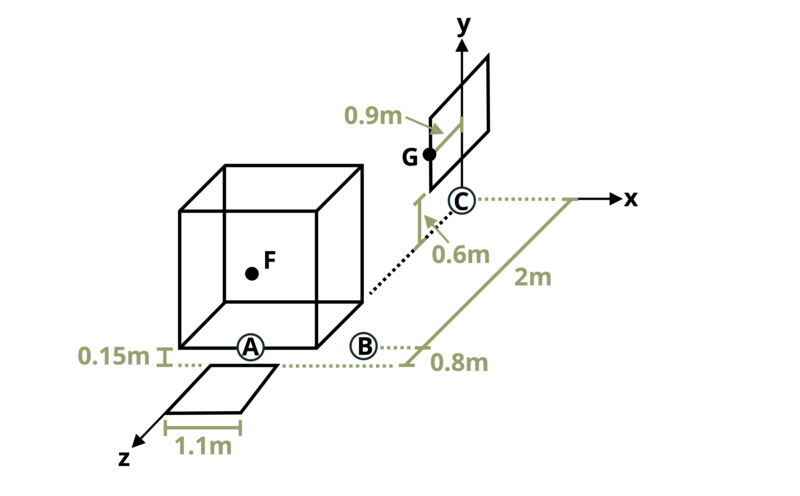
\includegraphics[keepaspectratio]{images/647.png}}
{[}Problem adapted from © Chris Galitz CC BY NC-SA 4.0{]}

\begin{Shaded}
\begin{Highlighting}[]
\NormalTok{\#| standalone: true}
\NormalTok{\#| viewerHeight: 600}
\NormalTok{\#| components: [viewer]}

\NormalTok{from shiny import App, render, ui, reactive}
\NormalTok{import random}
\NormalTok{import asyncio}
\NormalTok{import io}
\NormalTok{import math}
\NormalTok{import string}
\NormalTok{from datetime import datetime}
\NormalTok{from pathlib import Path}

\NormalTok{def generate\_random\_letters(length):}
\NormalTok{    \# Generate a random string of letters of specified length}
\NormalTok{    return "".join(random.choice(string.ascii\_lowercase) for \_ in range(length))}

\NormalTok{problem\_ID = "647"}
\NormalTok{W = reactive.Value("\_\_")}
\NormalTok{P = reactive.Value("\_\_")}
\NormalTok{attempts = ["Timestamp,Attempt,Answer1,Answer2,Answer3,Feedback\textbackslash{}n"]}

\NormalTok{app\_ui = ui.page\_fluid(}
\NormalTok{    \#ui.markdown("**Please enter your ID number from your instructor and click to generate your problem**"),}
\NormalTok{    \#ui.input\_text("ID", "", placeholder="Enter ID Number Here"),}
\NormalTok{    \#ui.input\_action\_button("generate\_problem", "Generate Problem", class\_="btn{-}primary"),}
\NormalTok{    ui.markdown("**Problem Statement**"),}
\NormalTok{    ui.output\_ui("ui\_problem\_statement"),}
\NormalTok{    ui.input\_text("answer1", "Your Answer 1 in units of kN", placeholder="Please enter your answer 1"),}
\NormalTok{    ui.input\_text("answer2", "Your Answer 2 in units of kN", placeholder="Please enter your answer 2"),}
\NormalTok{    ui.input\_text("answer3", "Your Answer 3 in units of kN", placeholder="Please enter your answer 2"),}

\NormalTok{    ui.input\_action\_button("submit", "Check Answers", class\_="btn{-}primary"),}
\NormalTok{    \#ui.download\_button("download", "Download File to Submit", class\_="btn{-}success"),}
\NormalTok{)}

\NormalTok{def server(input, output, session):}
\NormalTok{    \# Initialize a counter for attempts}
\NormalTok{    attempt\_counter = reactive.Value(0)}

\NormalTok{    @output}
\NormalTok{    @render.ui}
\NormalTok{    def ui\_problem\_statement():}
\NormalTok{        randomize\_vars()}
\NormalTok{        return [}
\NormalTok{            ui.markdown(}
\NormalTok{                f"A 3{-}wheeled forklift weighing W = \{W()\} kN centered at G is carrying an imbalanced load, P = \{P()\} kN, centered at F. determine the reactions at tires A, B, and C."}
\NormalTok{            )}
\NormalTok{        ]}

\NormalTok{    \#@reactive.Effect}
\NormalTok{    \#@reactive.event(input.generate\_problem)}
\NormalTok{    def randomize\_vars():}
\NormalTok{        random.seed(101)}
\NormalTok{        P.set(random.randrange(100,200,1)/10)}
\NormalTok{        W.set(random.randrange(10,30,1))}

\NormalTok{    @reactive.Effect}
\NormalTok{    @reactive.event(input.submit)}
\NormalTok{    def \_():}
\NormalTok{        attempt\_counter.set(}
\NormalTok{            attempt\_counter() + 1}
\NormalTok{        )  \# Increment the attempt counter on each submission.}

\NormalTok{        \# Calculate the instructor\textquotesingle{}s answer and determine if the user\textquotesingle{}s answer is correct.}
\NormalTok{        instr1 = ((0.6*W()+2.8*P())/2+(0.15*P())/0.55)/2}
\NormalTok{        instr2 = (0.6*W()+2.8*P())/2{-}instr1}
\NormalTok{        instr3 = P()+W(){-}instr1{-}instr2}

\NormalTok{        correct1 = math.isclose(float(input.answer1()), instr1, rel\_tol=0.01)}
\NormalTok{        correct2 = math.isclose(float(input.answer2()), instr2, rel\_tol=0.01)}
\NormalTok{        correct3 = math.isclose(float(input.answer3()), instr3, rel\_tol=0.01)}

\NormalTok{        if correct1 and correct2 and correct3:}
\NormalTok{            check = "All answers are correct."}
\NormalTok{        else:}
\NormalTok{            conditions = []}
\NormalTok{            for i, correct in enumerate([correct1, correct2, correct3], start=1):}
\NormalTok{                if correct:}
\NormalTok{                    conditions.append(f"correct for answer \{i\}")}
\NormalTok{                else:}
\NormalTok{                    conditions.append(f"incorrect for answer \{i\}")}
\NormalTok{            check = "; ".join(conditions) + "."}
        
\NormalTok{        correct\_indicator = "JL" if correct1 and correct2 and correct3 else "JG"}

\NormalTok{        random\_start = generate\_random\_letters(4)}
\NormalTok{        random\_middle = generate\_random\_letters(4)}
\NormalTok{        random\_end = generate\_random\_letters(4)}
\NormalTok{        \#encoded\_attempt = f"\{random\_start\}\{problem\_ID\}{-}\{random\_middle\}\{attempt\_counter()\}\{correct\_indicator\}{-}\{random\_end\}\{input.ID()\}"}

\NormalTok{        \#session.encoded\_attempt = reactive.Value(encoded\_attempt)}
\NormalTok{        attempts.append(f"\{datetime.now()\}, \{attempt\_counter()\}, \{input.answer1()\}, \{input.answer2()\}, \{check\}\textbackslash{}n")}

\NormalTok{        feedback = ui.markdown(f"Your answers of \{input.answer1()\}, \{input.answer2()\}, and \{input.answer3()\} are \{check\}.")}
\NormalTok{        m = ui.modal(feedback, title="Feedback", easy\_close=True)}
\NormalTok{        ui.modal\_show(m)}

\NormalTok{    \#@render.download(filename=lambda: f"Problem\_Log{-}\{problem\_ID\}{-}\{input.ID()\}.csv")}
\NormalTok{    async def download():}
\NormalTok{        final\_encoded = session.encoded\_attempt() if session.encoded\_attempt is not None else "No attempts"}
\NormalTok{        yield f"\{final\_encoded\}\textbackslash{}n\textbackslash{}n"}
\NormalTok{        yield "Timestamp,Attempt,Answer1,Answer2,Feedback\textbackslash{}n"}
\NormalTok{        for attempt in attempts[1:]:}
\NormalTok{            await asyncio.sleep(0.25)}
\NormalTok{            yield attempt}

\NormalTok{app = App(app\_ui, server)}
\end{Highlighting}
\end{Shaded}

\chapter*{Problem 1.8 - Equilibrium \& Reactions in
3D}\label{problem-1.8---equilibrium-reactions-in-3d}
\addcontentsline{toc}{chapter}{Problem 1.8 - Equilibrium \& Reactions in
3D}

\markboth{Problem 1.8 - Equilibrium \& Reactions in 3D}{Problem 1.8 -
Equilibrium \& Reactions in 3D}

\pandocbounded{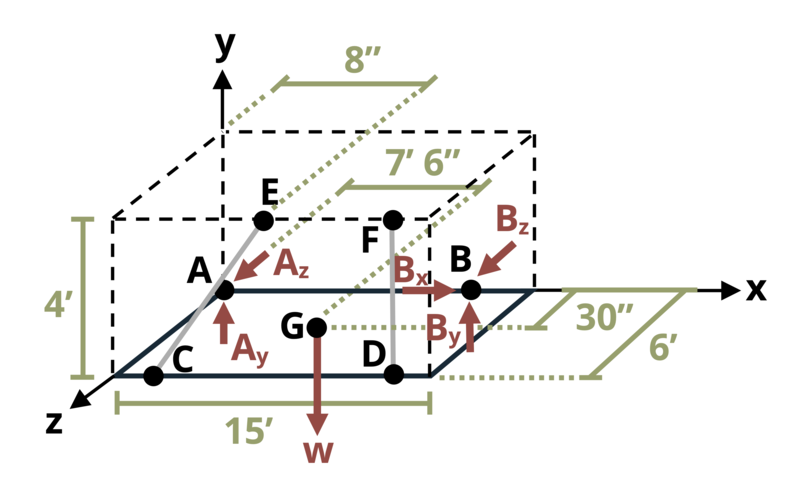
\includegraphics[keepaspectratio]{images/648.png}}
{[}Problem adapted from © Chris Galitz CC BY NC-SA 4.0{]}

\begin{Shaded}
\begin{Highlighting}[]
\NormalTok{\#| standalone: true}
\NormalTok{\#| viewerHeight: 600}
\NormalTok{\#| components: [viewer]}

\NormalTok{from shiny import App, render, ui, reactive}
\NormalTok{import random}
\NormalTok{import asyncio}
\NormalTok{import io}
\NormalTok{import math}
\NormalTok{import string}
\NormalTok{from datetime import datetime}
\NormalTok{from pathlib import Path}

\NormalTok{def generate\_random\_letters(length):}
\NormalTok{    \# Generate a random string of letters of specified length}
\NormalTok{    return "".join(random.choice(string.ascii\_lowercase) for \_ in range(length))}

\NormalTok{problem\_ID = "648"}
\NormalTok{w = reactive.Value("\_\_")}
\NormalTok{L = reactive.Value("\_\_")}
\NormalTok{weight = reactive.Value("\_\_")}
\NormalTok{attempts = ["Timestamp,Attempt,Answer1,Answer2,Answer3,Answer4,Feedback\textbackslash{}n"]}

\NormalTok{app\_ui = ui.page\_fluid(}
\NormalTok{    \#ui.markdown("**Please enter your ID number from your instructor and click to generate your problem**"),}
\NormalTok{    \#ui.input\_text("ID", "", placeholder="Enter ID Number Here"),}
\NormalTok{    \#ui.input\_action\_button("generate\_problem", "Generate Problem", class\_="btn{-}primary"),}
\NormalTok{    ui.markdown("**Problem Statement**"),}
\NormalTok{    ui.output\_ui("ui\_problem\_statement"),}
\NormalTok{    ui.input\_text("answer1", "Your Answer 1 in units of lb", placeholder="Please enter your answer 1"),}
\NormalTok{    ui.input\_text("answer2", "Your Answer 2 in units of lb", placeholder="Please enter your answer 2"),}
\NormalTok{    ui.input\_text("answer3", "Your Answer 3 in units of lb", placeholder="Please enter your answer 2"),}
\NormalTok{    ui.input\_text("answer4", "Your Answer 4 in units of lb", placeholder="Please enter your answer 2"),}

\NormalTok{    ui.input\_action\_button("submit", "Check Answers", class\_="btn{-}primary"),}
\NormalTok{    \#ui.download\_button("download", "Download File to Submit", class\_="btn{-}success"),}
\NormalTok{)}

\NormalTok{def server(input, output, session):}
\NormalTok{    \# Initialize a counter for attempts}
\NormalTok{    attempt\_counter = reactive.Value(0)}

\NormalTok{    @output}
\NormalTok{    @render.ui}
\NormalTok{    def ui\_problem\_statement():}
\NormalTok{        randomize\_vars()}
\NormalTok{        return [}
\NormalTok{            ui.markdown(}
\NormalTok{                f"An awning frame of width w = \{w()\} ft and length L = \{L()\} ft is attached to a wall by two anchors and two cables as shown. The awning weighs \{weight()\} lb. If the cables are installed such that their tensions are all equal, determine the tension, T, and each reaction at the anchors."}
\NormalTok{            )}
\NormalTok{        ]}

\NormalTok{    \#@reactive.Effect}
\NormalTok{    \#@reactive.event(input.generate\_problem)}
\NormalTok{    def randomize\_vars():}
\NormalTok{        random.seed(101)}
\NormalTok{        w.set(random.randrange(3,10,1))}
\NormalTok{        L.set(w()*random.randrange(20,30,1)/10)}
\NormalTok{        weight.set(random.randrange(50,100,1))}

\NormalTok{    @reactive.Effect}
\NormalTok{    @reactive.event(input.submit)}
\NormalTok{    def \_():}
\NormalTok{        attempt\_counter.set(}
\NormalTok{            attempt\_counter() + 1}
\NormalTok{        )  \# Increment the attempt counter on each submission.}

\NormalTok{        \# Calculate the instructor\textquotesingle{}s answer and determine if the user\textquotesingle{}s answer is correct.}
\NormalTok{        instr1 = 2.5*weight()/(1.106*w())}
\NormalTok{        instr2 = {-}0.3869*instr1}
\NormalTok{        Ay = (L()*0.552*instr1{-}7.5*weight())/({-}L())}
\NormalTok{        instr3 = weight(){-}Ay{-}instr1*(0.552){-}instr1*(0.554)}
\NormalTok{        Az = (L()*w()/7.238*instr1{-}0.0921*instr1*w()+w()*0.0461*instr1)/L()}
\NormalTok{        instr4 = {-}Az+instr1*w()/7.238+instr1*w()/7.22}

\NormalTok{        correct1 = math.isclose(float(input.answer1()), instr1, rel\_tol=0.01)}
\NormalTok{        correct2 = math.isclose(float(input.answer2()), instr2, rel\_tol=0.01)}
\NormalTok{        correct3 = math.isclose(float(input.answer3()), instr3, rel\_tol=0.01)}
\NormalTok{        correct4 = math.isclose(float(input.answer4()), instr4, rel\_tol=0.01)}


\NormalTok{        if correct1 and correct2 and correct3 and correct4:}
\NormalTok{            check = "All answers are correct."}
\NormalTok{        else:}
\NormalTok{            conditions = []}
\NormalTok{            for i, correct in enumerate([correct1, correct2, correct3, correct4], start=1):}
\NormalTok{                if correct:}
\NormalTok{                    conditions.append(f"correct for answer \{i\}")}
\NormalTok{                else:}
\NormalTok{                    conditions.append(f"incorrect for answer \{i\}")}
\NormalTok{            check = "; ".join(conditions) + "."}
        
\NormalTok{        correct\_indicator = "JL" if correct1 and correct2 and correct3 and correct4 else "JG"}

\NormalTok{        random\_start = generate\_random\_letters(4)}
\NormalTok{        random\_middle = generate\_random\_letters(4)}
\NormalTok{        random\_end = generate\_random\_letters(4)}
\NormalTok{        \#encoded\_attempt = f"\{random\_start\}\{problem\_ID\}{-}\{random\_middle\}\{attempt\_counter()\}\{correct\_indicator\}{-}\{random\_end\}\{input.ID()\}"}

\NormalTok{        \#session.encoded\_attempt = reactive.Value(encoded\_attempt)}
\NormalTok{        attempts.append(f"\{datetime.now()\}, \{attempt\_counter()\}, \{input.answer1()\}, \{input.answer2()\}, \{check\}\textbackslash{}n")}

\NormalTok{        feedback = ui.markdown(f"Your answers of \{input.answer1()\}, \{input.answer2()\}, \{input.answer3()\}, and \{input.answer4()\} are \{check\}.")}
\NormalTok{        m = ui.modal(feedback, title="Feedback", easy\_close=True)}
\NormalTok{        ui.modal\_show(m)}

\NormalTok{    \#@render.download(filename=lambda: f"Problem\_Log{-}\{problem\_ID\}{-}\{input.ID()\}.csv")}
\NormalTok{    async def download():}
\NormalTok{        final\_encoded = session.encoded\_attempt() if session.encoded\_attempt is not None else "No attempts"}
\NormalTok{        yield f"\{final\_encoded\}\textbackslash{}n\textbackslash{}n"}
\NormalTok{        yield "Timestamp,Attempt,Answer1,Answer2,Feedback\textbackslash{}n"}
\NormalTok{        for attempt in attempts[1:]:}
\NormalTok{            await asyncio.sleep(0.25)}
\NormalTok{            yield attempt}

\NormalTok{app = App(app\_ui, server)}
\end{Highlighting}
\end{Shaded}

\chapter*{Problem 1.9}\label{problem-1.9}
\addcontentsline{toc}{chapter}{Problem 1.9}

\markboth{Problem 1.9}{Problem 1.9}

\pandocbounded{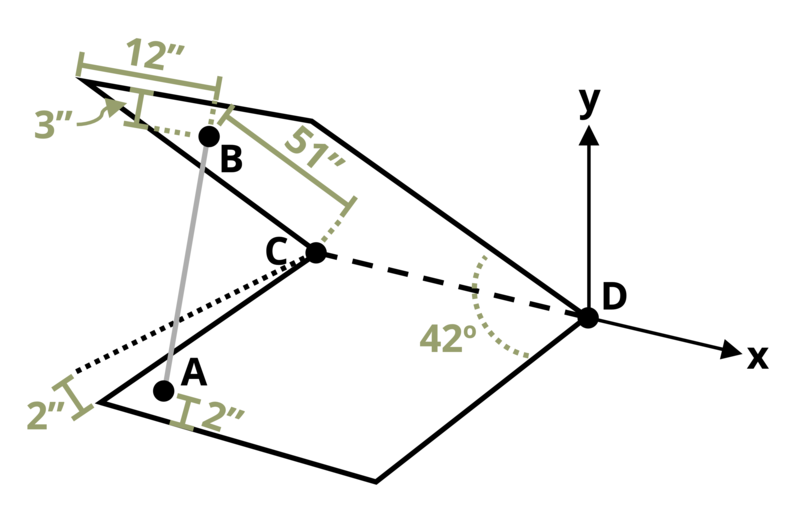
\includegraphics[keepaspectratio]{images/649.png}}
{[}Problem adapted from © Chris Galitz CC BY NC-SA 4.0{]}

\begin{Shaded}
\begin{Highlighting}[]
\NormalTok{\#| standalone: true}
\NormalTok{\#| viewerHeight: 600}
\NormalTok{\#| components: [viewer]}

\NormalTok{from shiny import App, render, ui, reactive}
\NormalTok{import random}
\NormalTok{import asyncio}
\NormalTok{import io}
\NormalTok{import math}
\NormalTok{import string}
\NormalTok{from datetime import datetime}
\NormalTok{from pathlib import Path}

\NormalTok{def generate\_random\_letters(length):}
\NormalTok{    \# Generate a random string of letters of specified length}
\NormalTok{    return "".join(random.choice(string.ascii\_lowercase) for \_ in range(length))}

\NormalTok{problem\_ID = "649"}
\NormalTok{w = reactive.Value("\_\_")}
\NormalTok{L = reactive.Value("\_\_")}
\NormalTok{weight = reactive.Value("\_\_")}
\NormalTok{attempts = ["Timestamp,Attempt,Answer1,Answer2,Answer3,Answer4,Answer5,Answer6,Feedback\textbackslash{}n"]}

\NormalTok{app\_ui = ui.page\_fluid(}
\NormalTok{    \#ui.markdown("**Please enter your ID number from your instructor and click to generate your problem**"),}
\NormalTok{    \#ui.input\_text("ID", "", placeholder="Enter ID Number Here"),}
\NormalTok{    \#ui.input\_action\_button("generate\_problem", "Generate Problem", class\_="btn{-}primary"),}
\NormalTok{    ui.markdown("**Problem Statement**"),}
\NormalTok{    ui.output\_ui("ui\_problem\_statement"),}
\NormalTok{    ui.input\_text("answer1", "Your Answer 1 in units of lb", placeholder="Please enter your answer 1"),}
\NormalTok{    ui.input\_text("answer2", "Your Answer 2 in units of lb", placeholder="Please enter your answer 2"),}
\NormalTok{    ui.input\_text("answer3", "Your Answer 3 in units of lb", placeholder="Please enter your answer 3"),}
\NormalTok{    ui.input\_text("answer4", "Your Answer 4 in units of lb", placeholder="Please enter your answer 4"),}
\NormalTok{    ui.input\_text("answer5", "Your Answer 5 in units of lb", placeholder="Please enter your answer 5"),}
\NormalTok{    ui.input\_text("answer6", "Your Answer 6 in units of lb", placeholder="Please enter your answer 6"),}


\NormalTok{    ui.input\_action\_button("submit", "Check Answers", class\_="btn{-}primary"),}
\NormalTok{    \#ui.download\_button("download", "Download File to Submit", class\_="btn{-}success"),}
\NormalTok{)}

\NormalTok{def server(input, output, session):}
\NormalTok{    \# Initialize a counter for attempts}
\NormalTok{    attempt\_counter = reactive.Value(0)}

\NormalTok{    @output}
\NormalTok{    @render.ui}
\NormalTok{    def ui\_problem\_statement():}
\NormalTok{        randomize\_vars()}
\NormalTok{        return [}
\NormalTok{            ui.markdown(}
\NormalTok{                f"During engine work, a car\textquotesingle{}s hood of length L = \{L()\} in. and width w = \{w()\} in., is propped up by rod AB. Hinges at C and D resist translation in the y{-} and z{-}directions but only D resists motion in the x{-}direction. If the hood weighs \{weight()\} lb, evenly distributed, determine the compressive force in rod AB and the reactions at C and D."}
\NormalTok{            )}
\NormalTok{        ]}

\NormalTok{    \#@reactive.Effect}
\NormalTok{    \#@reactive.event(input.generate\_problem)}
\NormalTok{    def randomize\_vars():}
\NormalTok{        random.seed(101)}
\NormalTok{        L.set(random.randrange(50,70,1))}
\NormalTok{        w.set(L()+random.randrange(10,20,1))}
\NormalTok{        weight.set(random.randrange(30,80,1))}

\NormalTok{    @reactive.Effect}
\NormalTok{    @reactive.event(input.submit)}
\NormalTok{    def \_():}
\NormalTok{        attempt\_counter.set(}
\NormalTok{            attempt\_counter() + 1}
\NormalTok{        )  \# Increment the attempt counter on each submission.}

\NormalTok{        \# Calculate the instructor\textquotesingle{}s answer and determine if the user\textquotesingle{}s answer is correct.}
\NormalTok{        RDB = [{-}w()+12, 34.13, 37.9]}
\NormalTok{        RDA = [{-}w()+6, 0, L(){-}2]}
\NormalTok{        RDC = [{-}w(), 0, 0]}
\NormalTok{        RDG = [{-}w()/2, L()/2*0.6691, L()/2*0.7431]}
\NormalTok{        def vector\_subtraction(RDB, RDA):}
\NormalTok{            return [x {-} y for x, y in zip(RDB, RDA)]}
\NormalTok{        RAB = vector\_subtraction(RDB,RDA)}
\NormalTok{        def vector\_magnitude(RAB):}
\NormalTok{            return math.sqrt(sum(x ** 2 for x in RAB))}
\NormalTok{        RABmag = vector\_magnitude(RAB)}
\NormalTok{        FbarAB = [x/RABmag for x in RAB]}
\NormalTok{        comp1 = RDB[1]*FbarAB[2]{-}RDB[2]*FbarAB[1]}
\NormalTok{        comp2 = RDB[2]*FbarAB[0]{-}RDB[0]*FbarAB[2]}
\NormalTok{        comp3 = RDB[0]*FbarAB[1]{-}RDB[1]*FbarAB[0]}
\NormalTok{        FABCross = [comp1, comp2, comp3]}
\NormalTok{        Weightj = [0, {-}weight(), 0]}
\NormalTok{        comp4 = RDG[1]*Weightj[2]{-}RDG[2]*Weightj[1]}
\NormalTok{        comp5 = RDG[2]*Weightj[0]{-}RDG[0]*Weightj[2]}
\NormalTok{        comp6 = RDG[0]*Weightj[1]{-}RDG[1]*Weightj[0]}
\NormalTok{        RDGCross = [comp4, comp5, comp6]}
\NormalTok{        instr1 = comp4/comp1}
\NormalTok{        Cract = [0,1,1]}
\NormalTok{        comp7 = RDC[1]*Cract[2]{-}RDC[2]*Cract[1]}
\NormalTok{        comp8 = RDC[2]*Cract[0]{-}RDC[0]*Cract[2]}
\NormalTok{        comp9 = RDC[0]*Cract[1]{-}RDC[1]*Cract[0]}
\NormalTok{        RDCCross = [comp7, comp8, comp9]}
\NormalTok{        instr2 = comp2*instr1/comp8}
\NormalTok{        instr3 = (comp3*instr1{-}comp6)/comp9}
\NormalTok{        instr4 = {-}FbarAB[0]*instr1}
\NormalTok{        instr5 = {-}FbarAB[1]*instr1+weight(){-}instr3}
\NormalTok{        instr6 = {-}FbarAB[2]{-}instr2 }
  
\NormalTok{        correct1 = math.isclose(float(input.answer1()), instr1, rel\_tol=0.01)}
\NormalTok{        correct2 = math.isclose(float(input.answer2()), instr2, rel\_tol=0.01)}
\NormalTok{        correct3 = math.isclose(float(input.answer3()), instr3, rel\_tol=0.01)}
\NormalTok{        correct4 = math.isclose(float(input.answer4()), instr4, rel\_tol=0.01)}
\NormalTok{        correct5 = math.isclose(float(input.answer5()), instr5, rel\_tol=0.01)}
\NormalTok{        correct6 = math.isclose(float(input.answer6()), instr6, rel\_tol=0.01)}

\NormalTok{        if correct1 and correct2 and correct3 and correct4 and correct5 and correct6:}
\NormalTok{            check = "All answers are correct."}
\NormalTok{        else:}
\NormalTok{            conditions = []}
\NormalTok{            for i, correct in enumerate([correct1, correct2, correct3, correct4, correct5, correct6], start=1):}
\NormalTok{                if correct:}
\NormalTok{                    conditions.append(f"correct for answer \{i\}")}
\NormalTok{                else:}
\NormalTok{                    conditions.append(f"incorrect for answer \{i\}")}
\NormalTok{            check = "; ".join(conditions) + "."}
        
\NormalTok{        correct\_indicator = "JL" if correct1 and correct2 and correct3 and correct4 and correct5 and correct6 else "JG"}

\NormalTok{        random\_start = generate\_random\_letters(4)}
\NormalTok{        random\_middle = generate\_random\_letters(4)}
\NormalTok{        random\_end = generate\_random\_letters(4)}
\NormalTok{        \#encoded\_attempt = f"\{random\_start\}\{problem\_ID\}{-}\{random\_middle\}\{attempt\_counter()\}\{correct\_indicator\}{-}\{random\_end\}\{input.ID()\}"}

\NormalTok{        \#session.encoded\_attempt = reactive.Value(encoded\_attempt)}
\NormalTok{        attempts.append(f"\{datetime.now()\}, \{attempt\_counter()\}, \{input.answer1()\}, \{input.answer2()\}, \{check\}\textbackslash{}n")}

\NormalTok{        feedback = ui.markdown(f"Your answers of \{input.answer1()\}, \{input.answer2()\}, \{input.answer3()\}, \{input.answer4()\}, \{input.answer5()\}, and \{input.answer6()\} are \{check\}.")}
\NormalTok{        m = ui.modal(feedback, title="Feedback", easy\_close=True)}
\NormalTok{        ui.modal\_show(m)}

\NormalTok{    \#@render.download(filename=lambda: f"Problem\_Log{-}\{problem\_ID\}{-}\{input.ID()\}.csv")}
\NormalTok{    async def download():}
\NormalTok{        final\_encoded = session.encoded\_attempt() if session.encoded\_attempt is not None else "No attempts"}
\NormalTok{        yield f"\{final\_encoded\}\textbackslash{}n\textbackslash{}n"}
\NormalTok{        yield "Timestamp,Attempt,Answer1,Answer2,Answer3,Answer4,Answer5,Answer6,Feedback\textbackslash{}n"}
\NormalTok{        for attempt in attempts[1:]:}
\NormalTok{            await asyncio.sleep(0.25)}
\NormalTok{            yield attempt}

\NormalTok{app = App(app\_ui, server)}
\end{Highlighting}
\end{Shaded}

\part{Chapter 2 Problems}

\chapter*{Problem 2.1 - Average Normal
Stress}\label{problem-2.1---average-normal-stress}
\addcontentsline{toc}{chapter}{Problem 2.1 - Average Normal Stress}

\markboth{Problem 2.1 - Average Normal Stress}{Problem 2.1 - Average
Normal Stress}

\begin{figure}[H]

{\centering \pandocbounded{
\includegraphics[keepaspectratio]{images/138.png}}

}

\caption{Figure 1: A series of solid circular bars are loaded with three
loads}

\end{figure}%

{[}Problem adapted from © Kurt Gramoll CC BY NC-SA 4.0{]}

\begin{Shaded}
\begin{Highlighting}[]
\NormalTok{\#| standalone: true}
\NormalTok{\#| viewerHeight: 600}
\NormalTok{\#| components: [viewer]}

\NormalTok{from shiny import App, render, ui, reactive}
\NormalTok{import random}
\NormalTok{import asyncio}
\NormalTok{import io}
\NormalTok{import math}
\NormalTok{import string}
\NormalTok{from datetime import datetime}
\NormalTok{from pathlib import Path}


\NormalTok{def generate\_random\_letters(length):}
\NormalTok{    \# Generate a random string of letters of specified length}
\NormalTok{    return \textquotesingle{}\textquotesingle{}.join(random.choice(string.ascii\_lowercase) for \_ in range(length))  }

\NormalTok{problem\_ID="138"}
\NormalTok{F1=reactive.Value("\_\_")}
\NormalTok{F2=reactive.Value("\_\_")}
\NormalTok{F3=reactive.Value("\_\_")}
\NormalTok{d1=8}
\NormalTok{d2=6}
\NormalTok{d3=10}
\NormalTok{attempts=["Timestamp,Attempt,Answer,Feedback\textbackslash{}n"]}

\NormalTok{app\_ui = ui.page\_fluid(}
\NormalTok{    \#ui.markdown("**Please enter your ID number from your instructor and click to generate your problem**"),}
\NormalTok{    \#ui.input\_text("ID","", placeholder="Enter ID Number Here"),}
\NormalTok{    \#ui.input\_action\_button("generate\_problem", "Generate Problem", class\_="btn{-}primary"),}
\NormalTok{    ui.markdown("**Problem Statement**"),}
\NormalTok{    ui.output\_ui("ui\_problem\_statement"),}
\NormalTok{    ui.input\_text("answer","Your Answer in units of MPa", placeholder="Please enter your answer"),}
\NormalTok{    ui.input\_action\_button("submit", "Check Answer", class\_="btn{-}primary"),}
\NormalTok{    \#ui.download\_button("download", "Download File to Submit", class\_="btn{-}success"),}
\NormalTok{)}


\NormalTok{def server(input, output, session):}
\NormalTok{    \# Initialize a counter for attempts}
\NormalTok{    attempt\_counter = reactive.Value(0)}
    
\NormalTok{    @output}
\NormalTok{    @render.ui}
\NormalTok{    def ui\_problem\_statement():}
\NormalTok{        randomize\_vars()}
\NormalTok{        return[ui.markdown(f"A series of solid circular bars are loaded with three loads as shown, F\textless{}sub\textgreater{}1\textless{}/sub\textgreater{} = \{F1()\} N, F\textless{}sub\textgreater{}2\textless{}/sub\textgreater{} = \{F2()\} N, and F\textless{}sub\textgreater{}3\textless{}/sub\textgreater{} = \{F3()\} N. What is the largest absolute normal stress in any bar?")]}
     
\NormalTok{    \#@reactive.Effect}
\NormalTok{    \#@reactive.event(input.generate\_problem)}
\NormalTok{    def randomize\_vars():}
\NormalTok{        random.seed(101)}
\NormalTok{        F1.set(random.randrange(50, 70, 1))}
\NormalTok{        F2.set(random.randrange(10, 30, 1))}
\NormalTok{        F3.set(F1(){-}F2())}
        

\NormalTok{    @reactive.Effect}
\NormalTok{    @reactive.event(input.submit)}
\NormalTok{    def \_():}
\NormalTok{        attempt\_counter.set(attempt\_counter() + 1)  \# Increment the attempt counter on each submission.}
        
\NormalTok{        \# Calculate the instructor\textquotesingle{}s answer and determine if the user\textquotesingle{}s answer is correct.}
\NormalTok{        instr= (F1()/(math.pi*(d2/(1000*2))**2))/10**6}
        
\NormalTok{        if math.isclose(float(input.answer()), instr, rel\_tol=0.01):}
\NormalTok{            check = "*Correct*"}
\NormalTok{            correct\_indicator = "JL"}
\NormalTok{        else:}
\NormalTok{            check = "*Not Correct.*"}
\NormalTok{            correct\_indicator = "JG"}

\NormalTok{        \# Generate random parts for the encoded attempt.}
\NormalTok{        random\_start = generate\_random\_letters(4)}
\NormalTok{        random\_middle = generate\_random\_letters(4)}
\NormalTok{        random\_end = generate\_random\_letters(4)}
\NormalTok{        \#encoded\_attempt = f"\{random\_start\}\{problem\_ID\}{-}\{random\_middle\}\{attempt\_counter()\}\{correct\_indicator\}{-}\{random\_end\}\{input.ID()\}"}

\NormalTok{        \# Store the most recent encoded attempt in a reactive value so it persists across submissions}
\NormalTok{        \#session.encoded\_attempt = reactive.Value(encoded\_attempt)}

\NormalTok{        \# Append the attempt data to the attempts list without the encoded attempt}
\NormalTok{        attempts.append(f"\{datetime.now()\}, \{attempt\_counter()\}, \{input.answer()\}, \{check\}\textbackslash{}n")}

\NormalTok{        \# Show feedback to the user.}
\NormalTok{        feedback = ui.markdown(f"Your answer of \{input.answer()\} is \{check\}.")}
\NormalTok{        m = ui.modal(}
\NormalTok{            feedback,}
\NormalTok{            title="Feedback",}
\NormalTok{            easy\_close=True}
\NormalTok{        )}
\NormalTok{        ui.modal\_show(m)}

\NormalTok{    \#@render.download(filename=lambda: f"Problem\_Log{-}\{problem\_ID\}{-}\{input.ID()\}.csv")}
\NormalTok{    async def download():}
\NormalTok{        \# Start the CSV with the encoded attempt (without label)}
\NormalTok{        final\_encoded = session.encoded\_attempt() if session.encoded\_attempt is not None else "No attempts"}
\NormalTok{        yield f"\{final\_encoded\}\textbackslash{}n\textbackslash{}n"}
        
\NormalTok{        \# Write the header for the remaining CSV data once}
\NormalTok{        yield "Timestamp,Attempt,Answer,Feedback\textbackslash{}n"}
        
\NormalTok{        \# Write the attempts data, ensure that the header from the attempts list is not written again}
\NormalTok{        for attempt in attempts[1:]:  \# Skip the first element which is the header}
\NormalTok{            await asyncio.sleep(0.25)  \# This delay may not be necessary; adjust as needed}
\NormalTok{            yield attempt}


\NormalTok{\# App installation}
\NormalTok{app = App(app\_ui, server)}
\end{Highlighting}
\end{Shaded}

\chapter*{Problem 2.2 - Average Normal
Stress}\label{problem-2.2---average-normal-stress}
\addcontentsline{toc}{chapter}{Problem 2.2 - Average Normal Stress}

\markboth{Problem 2.2 - Average Normal Stress}{Problem 2.2 - Average
Normal Stress}


\includegraphics[width=8.52083in,height=\textheight,keepaspectratio]{images/139.png}
{[}Problem adapted from © Kurt Gramoll CC BY NC-SA 4.0{]}

\begin{Shaded}
\begin{Highlighting}[]
\NormalTok{\#| standalone: true}
\NormalTok{\#| viewerHeight: 600}
\NormalTok{\#| components: [viewer]}

\NormalTok{from shiny import App, render, ui, reactive}
\NormalTok{import random}
\NormalTok{import asyncio}
\NormalTok{import io}
\NormalTok{import math}
\NormalTok{import string}
\NormalTok{from datetime import datetime}
\NormalTok{from pathlib import Path}

\NormalTok{def generate\_random\_letters(length):}
\NormalTok{    \# Generate a random string of letters of specified length}
\NormalTok{    return \textquotesingle{}\textquotesingle{}.join(random.choice(string.ascii\_lowercase) for \_ in range(length))  }

\NormalTok{problem\_ID="139"}
\NormalTok{L1=reactive.Value("\_\_")}
\NormalTok{L2=reactive.Value("\_\_")}
\NormalTok{FA=reactive.Value("\_\_")}
\NormalTok{FB=reactive.Value("\_\_")}
\NormalTok{E = 30*10**6}
  
\NormalTok{attempts=["Timestamp,Attempt,Answer,Feedback\textbackslash{}n"]}

\NormalTok{app\_ui = ui.page\_fluid(}
\NormalTok{    \#ui.markdown("**Please enter your ID number from your instructor and click to generate your problem**"),}
\NormalTok{    \#ui.input\_text("ID","", placeholder="Enter ID Number Here"),}
\NormalTok{    \#ui.input\_action\_button("generate\_problem", "Generate Problem", class\_="btn{-}primary"),}
\NormalTok{    ui.markdown("**Problem Statement**"),}
\NormalTok{    ui.output\_ui("ui\_problem\_statement"),}
\NormalTok{    ui.input\_text("answer","Your Answer in units of psi", placeholder="Please enter your answer"),}
\NormalTok{    ui.input\_action\_button("submit", "Check Answer", class\_="btn{-}primary"),}
\NormalTok{    \#ui.download\_button("download", "Download File to Submit", class\_="btn{-}success"),}
\NormalTok{)}

\NormalTok{def server(input, output, session):}
\NormalTok{    \# Initialize a counter for attempts}
\NormalTok{    attempt\_counter = reactive.Value(0)}

\NormalTok{    @output}
\NormalTok{    @render.ui}
\NormalTok{    def ui\_problem\_statement():}
\NormalTok{        randomize\_vars()}
\NormalTok{        return[ui.markdown(f"Two cylinders are stacked on top of one another and two forces are applied at the top surface and at the joint between the cylinders as shown. If L\textless{}sub\textgreater{}1\textless{}/sub\textgreater{} = \{L1()\} in., L\textless{}sub\textgreater{}2\textless{}/sub\textgreater{} = \{L2()\} in., F\textless{}sub\textgreater{}A\textless{}/sub\textgreater{} = \{FA()\} lb, and F\textless{}sub\textgreater{}B\textless{}/sub\textgreater{} = \{FB()\} lb, determine the average normal stress in cylinder B. Enter a positive answer for tensile stress or a negative answer for compressive stress. ")]}
    
\NormalTok{    \#@reactive.Effect}
\NormalTok{    \#@reactive.event(input.generate\_problem)}
\NormalTok{    def randomize\_vars():}
\NormalTok{        random.seed(101)}
\NormalTok{        FA.set(random.randrange(300, 700, 10))}
\NormalTok{        FB.set(random.randrange(100, 300, 10))}
\NormalTok{        L1.set(random.randrange(2, 7, 1))}
\NormalTok{        L2.set(round(L1() * 1.3,1))}
        
\NormalTok{    @reactive.Effect}
\NormalTok{    @reactive.event(input.submit)}
\NormalTok{    def \_():}
\NormalTok{        attempt\_counter.set(attempt\_counter() + 1)  \# Increment the attempt counter on each submission.}
    
\NormalTok{        instr = {-}(FA()+FB())/(math.pi*1.5**2)}
\NormalTok{        if math.isclose(float(input.answer()), instr, rel\_tol=0.01):}
\NormalTok{            check = "*Correct*"}
\NormalTok{            correct\_indicator = "JL"}
\NormalTok{        else:}
\NormalTok{            check = "*Not Correct.*"}
\NormalTok{            correct\_indicator = "JG"}

\NormalTok{        \# Generate random parts for the encoded attempt.}
\NormalTok{        random\_start = generate\_random\_letters(4)}
\NormalTok{        random\_middle = generate\_random\_letters(4)}
\NormalTok{        random\_end = generate\_random\_letters(4)}
\NormalTok{        \#encoded\_attempt = f"\{random\_start\}\{problem\_ID\}{-}\{random\_middle\}\{attempt\_counter()\}\{correct\_indicator\}{-}\{random\_end\}\{input.ID()\}"}

\NormalTok{        \# Store the most recent encoded attempt in a reactive value so it persists across submissions}
\NormalTok{        \#session.encoded\_attempt = reactive.Value(encoded\_attempt)}

\NormalTok{        \# Append the attempt data to the attempts list without the encoded attempt}
\NormalTok{        attempts.append(f"\{datetime.now()\}, \{attempt\_counter()\}, \{input.answer()\}, \{check\}\textbackslash{}n")}

\NormalTok{        \# Show feedback to the user.}
\NormalTok{        feedback = ui.markdown(f"Your answer of \{input.answer()\} is \{check\}.")}
\NormalTok{        m = ui.modal(}
\NormalTok{            feedback,}
\NormalTok{            title="Feedback",}
\NormalTok{            easy\_close=True}
\NormalTok{        )}
\NormalTok{        ui.modal\_show(m)}

\NormalTok{    \#@render.download(filename=lambda: f"Problem\_Log{-}\{problem\_ID\}{-}\{input.ID()\}.csv")}
\NormalTok{    async def download():}
\NormalTok{        \# Start the CSV with the encoded attempt (without label)}
\NormalTok{        final\_encoded = session.encoded\_attempt() if session.encoded\_attempt is not None else "No attempts"}
\NormalTok{        yield f"\{final\_encoded\}\textbackslash{}n\textbackslash{}n"}
        
\NormalTok{        \# Write the header for the remaining CSV data once}
\NormalTok{        yield "Timestamp,Attempt,Answer,Feedback\textbackslash{}n"}
        
\NormalTok{        \# Write the attempts data, ensure that the header from the attempts list is not written again}
\NormalTok{        for attempt in attempts[1:]:  \# Skip the first element which is the header}
\NormalTok{            await asyncio.sleep(0.25)  \# This delay may not be necessary; adjust as needed}
\NormalTok{            yield attempt}

\NormalTok{\# App installation}
\NormalTok{app = App(app\_ui, server)}
\end{Highlighting}
\end{Shaded}

\chapter*{Problem 2.3 - Average Normal
Stress}\label{problem-2.3---average-normal-stress}
\addcontentsline{toc}{chapter}{Problem 2.3 - Average Normal Stress}

\markboth{Problem 2.3 - Average Normal Stress}{Problem 2.3 - Average
Normal Stress}


\includegraphics[width=9.33333in,height=\textheight,keepaspectratio]{images/144.png}
{[}Problem adapted from © Kurt Gramoll CC BY NC-SA 4.0{]}

\begin{Shaded}
\begin{Highlighting}[]
\NormalTok{\#| standalone: true}
\NormalTok{\#| viewerHeight: 600}
\NormalTok{\#| components: [viewer]}

\NormalTok{from shiny import App, render, ui, reactive}
\NormalTok{import random}
\NormalTok{import asyncio}
\NormalTok{import io}
\NormalTok{import math}
\NormalTok{import string}
\NormalTok{from datetime import datetime}
\NormalTok{from pathlib import Path}

\NormalTok{def generate\_random\_letters(length):}
\NormalTok{    \# Generate a random string of letters of specified length}
\NormalTok{    return \textquotesingle{}\textquotesingle{}.join(random.choice(string.ascii\_lowercase) for \_ in range(length))}

\NormalTok{problem\_ID="144"}
\NormalTok{F=reactive.Value("\_\_")}
\NormalTok{d1=reactive.Value("\_\_")}
\NormalTok{d2=reactive.Value("\_\_")}

\NormalTok{attempts=["Timestamp,Attempt,Answer,Feedback\textbackslash{}n"]}

\NormalTok{app\_ui = ui.page\_fluid(}
\NormalTok{    \#ui.markdown("**Please enter your ID number from your instructor and click to generate your problem**"),}
\NormalTok{    \#ui.input\_text("ID","", placeholder="Enter ID Number Here"),}
\NormalTok{    \#ui.input\_action\_button("generate\_problem", "Generate Problem", class\_="btn{-}primary"),}
\NormalTok{    ui.markdown("**Problem Statement**"),}
\NormalTok{    ui.output\_ui("ui\_problem\_statement"),}
\NormalTok{    ui.input\_text("answer","Your Answer in units of psi", placeholder="Please enter your answer"),}
\NormalTok{    ui.input\_action\_button("submit", "Check Answer", class\_="btn{-}primary"),}
\NormalTok{    \#ui.download\_button("download", "Download File to Submit", class\_="btn{-}success"),}
\NormalTok{)}


\NormalTok{def server(input, output, session):}
\NormalTok{    \# Initialize a counter for attempts}
\NormalTok{    attempt\_counter = reactive.Value(0)}

\NormalTok{    @output}
\NormalTok{    @render.ui}
\NormalTok{    def ui\_problem\_statement():}
\NormalTok{        randomize\_vars()}
\NormalTok{        return[ui.markdown(f"A plastic cylindrical peg is constrained by a metal cap as shown. An axial load of F = \{F()\} lb is applied to the peg. If d\textless{}sub\textgreater{}1\textless{}/sub\textgreater{} = \{d1()\} in and d\textless{}sub\textgreater{}2\textless{}/sub\textgreater{} = \{d2()\} in, determine the largest normal stress in the peg. Assume the axial load is evenly distributed across the peg and that the metal cap is fixed and does not move.")]}
    
\NormalTok{    \#@reactive.Effect}
\NormalTok{    \#@reactive.event(input.generate\_problem)}
\NormalTok{    def randomize\_vars():}
\NormalTok{        random.seed(101)}
\NormalTok{        F.set(random.randrange(20, 80, 5))}
\NormalTok{        d1.set(random.randrange(3, 8, 1)/10)}
\NormalTok{        d2.set(round(d1() * 1.6, 2))}
        
 
\NormalTok{    @reactive.Effect}
\NormalTok{    @reactive.event(input.submit)}
\NormalTok{    def \_():}
\NormalTok{        attempt\_counter.set(attempt\_counter() + 1)  \# Increment the attempt counter on each submission.}
\NormalTok{        instr= F()/(math.pi*((d1()/2)**2))}
\NormalTok{        \#check=math.isclose(float(input.answer()),instr,rel\_tol=0.001)}
        
\NormalTok{        if math.isclose(float(input.answer()), instr, rel\_tol=0.01):}
\NormalTok{            check = "*Correct*"}
\NormalTok{            correct\_indicator = "JL"}
\NormalTok{        else:}
\NormalTok{            check = "*Not Correct.*"}
\NormalTok{            correct\_indicator = "JG"}

\NormalTok{        \# Generate random parts for the encoded attempt.}
\NormalTok{        random\_start = generate\_random\_letters(4)}
\NormalTok{        random\_middle = generate\_random\_letters(4)}
\NormalTok{        random\_end = generate\_random\_letters(4)}
\NormalTok{        \#encoded\_attempt = f"\{random\_start\}\{problem\_ID\}{-}\{random\_middle\}\{attempt\_counter()\}\{correct\_indicator\}{-}\{random\_end\}\{input.ID()\}"}

\NormalTok{        \# Store the most recent encoded attempt in a reactive value so it persists across submissions}
\NormalTok{        \#session.encoded\_attempt = reactive.Value(encoded\_attempt)}

\NormalTok{        \# Append the attempt data to the attempts list without the encoded attempt}
\NormalTok{        attempts.append(f"\{datetime.now()\}, \{attempt\_counter()\}, \{input.answer()\}, \{check\}\textbackslash{}n")}

\NormalTok{        \# Show feedback to the user.}
\NormalTok{        feedback = ui.markdown(f"Your answer of \{input.answer()\} is \{check\}.")}
\NormalTok{        m = ui.modal(}
\NormalTok{            feedback,}
\NormalTok{            title="Feedback",}
\NormalTok{            easy\_close=True}
\NormalTok{        )}
\NormalTok{        ui.modal\_show(m)}

\NormalTok{    \#@render.download(filename=lambda: f"Problem\_Log{-}\{problem\_ID\}{-}\{input.ID()\}.csv")}
\NormalTok{    async def download():}
\NormalTok{        \# Start the CSV with the encoded attempt (without label)}
\NormalTok{        final\_encoded = session.encoded\_attempt() if session.encoded\_attempt is not None else "No attempts"}
\NormalTok{        yield f"\{final\_encoded\}\textbackslash{}n\textbackslash{}n"}
        
\NormalTok{        \# Write the header for the remaining CSV data once}
\NormalTok{        yield "Timestamp,Attempt,Answer,Feedback\textbackslash{}n"}
        
\NormalTok{        \# Write the attempts data, ensure that the header from the attempts list is not written again}
\NormalTok{        for attempt in attempts[1:]:  \# Skip the first element which is the header}
\NormalTok{            await asyncio.sleep(0.25)  \# This delay may not be necessary; adjust as needed}
\NormalTok{            yield attempt}


\NormalTok{\# App installation}
\NormalTok{app = App(app\_ui, server)}
\end{Highlighting}
\end{Shaded}

\chapter*{Problem 2.4 - Average Normal
Stress}\label{problem-2.4---average-normal-stress}
\addcontentsline{toc}{chapter}{Problem 2.4 - Average Normal Stress}

\markboth{Problem 2.4 - Average Normal Stress}{Problem 2.4 - Average
Normal Stress}


\includegraphics[width=15.48958in,height=\textheight,keepaspectratio]{images/146.png}
{[}Problem adapted from © Kurt Gramoll CC BY NC-SA 4.0{]}

\begin{Shaded}
\begin{Highlighting}[]
\NormalTok{\#| standalone: true}
\NormalTok{\#| viewerHeight: 600}
\NormalTok{\#| components: [viewer]}

\NormalTok{from shiny import App, render, ui, reactive}
\NormalTok{import random}
\NormalTok{import asyncio}
\NormalTok{import io}
\NormalTok{import math}
\NormalTok{import string}
\NormalTok{from datetime import datetime}
\NormalTok{from pathlib import Path}


\NormalTok{def generate\_random\_letters(length):}
\NormalTok{    \# Generate a random string of letters of specified length}
\NormalTok{    return \textquotesingle{}\textquotesingle{}.join(random.choice(string.ascii\_lowercase) for \_ in range(length)) }

\NormalTok{problem\_ID="146"}
\NormalTok{W=reactive.Value("\_\_")}
\NormalTok{d=reactive.Value("\_\_")}
\NormalTok{angle1=math.radians(45)}
\NormalTok{angle2=math.radians(30)}
\NormalTok{angle3=math.radians(75)}

\NormalTok{attempts=["Timestamp,Attempt,Answer,Feedback\textbackslash{}n"]}

\NormalTok{app\_ui = ui.page\_fluid(}
\NormalTok{    \#ui.markdown("**Please enter your ID number from your instructor and click to generate your problem**"),}
\NormalTok{    \#ui.input\_text("ID","", placeholder="Enter ID Number Here"),}
\NormalTok{    \#ui.input\_action\_button("generate\_problem", "Generate Problem", class\_="btn{-}primary"),}
\NormalTok{    ui.markdown("**Problem Statement**"),}
\NormalTok{    ui.output\_ui("ui\_problem\_statement"),}
\NormalTok{    ui.input\_text("answer","Your Answer in units of MPa", placeholder="Please enter your answer"),}
\NormalTok{    ui.input\_action\_button("submit", "Check Answer", class\_="btn{-}primary"),}
\NormalTok{    \#ui.download\_button("download", "Download File to Submit", class\_="btn{-}success"),}
\NormalTok{)}


\NormalTok{def server(input, output, session):}
\NormalTok{    \# Initialize a counter for attempts}
\NormalTok{    attempt\_counter = reactive.Value(0)}

\NormalTok{    @output}
\NormalTok{    @render.ui}
\NormalTok{    def ui\_problem\_statement():}
\NormalTok{        randomize\_vars()}
\NormalTok{        return[ui.markdown(f"A crate weighing \{W()\} kN is suspended by a set of cables. The diameter of each cable is \{d()\}  mm. What is the maximum stress in any cable, that is the highest average normal stress, excluding the cable attached to the crate.")]}
    
\NormalTok{    \#@reactive.Effect}
\NormalTok{    \#@reactive.event(input.generate\_problem)}
\NormalTok{    def randomize\_vars():}
\NormalTok{        random.seed(101)}
\NormalTok{        W.set(random.randrange(30, 90, 1))}
\NormalTok{        d.set(random.randrange(20, 60, 1))}
        

\NormalTok{    @reactive.Effect}
\NormalTok{    @reactive.event(input.submit)}
\NormalTok{    def \_():}
\NormalTok{        attempt\_counter.set(attempt\_counter() + 1)  \# Increment the attempt counter on each submission.}
    
\NormalTok{        R1 = W()/(((math.cos(angle1)/math.cos(angle2))*math.sin(angle2))+math.sin(angle1))}
\NormalTok{        instr = (R1*10**3/(math.pi*((d()/(1000*2))**2)))/10**6}
\NormalTok{        if math.isclose(float(input.answer()), instr, rel\_tol=0.01):}
\NormalTok{            check = "*Correct*"}
\NormalTok{            correct\_indicator = "JL"}
\NormalTok{        else:}
\NormalTok{            check = "*Not Correct.*"}
\NormalTok{            correct\_indicator = "JG"}

\NormalTok{        \# Generate random parts for the encoded attempt.}
\NormalTok{        random\_start = generate\_random\_letters(4)}
\NormalTok{        random\_middle = generate\_random\_letters(4)}
\NormalTok{        random\_end = generate\_random\_letters(4)}
\NormalTok{        \#encoded\_attempt = f"\{random\_start\}\{problem\_ID\}{-}\{random\_middle\}\{attempt\_counter()\}\{correct\_indicator\}{-}\{random\_end\}\{input.ID()\}"}

\NormalTok{        \# Store the most recent encoded attempt in a reactive value so it persists across submissions}
\NormalTok{        \#session.encoded\_attempt = reactive.Value(encoded\_attempt)}

\NormalTok{        \# Append the attempt data to the attempts list without the encoded attempt}
\NormalTok{        attempts.append(f"\{datetime.now()\}, \{attempt\_counter()\}, \{input.answer()\}, \{check\}\textbackslash{}n")}

\NormalTok{        \# Show feedback to the user.}
\NormalTok{        feedback = ui.markdown(f"Your answer of \{input.answer()\} is \{check\}.")}
\NormalTok{        m = ui.modal(}
\NormalTok{            feedback,}
\NormalTok{            title="Feedback",}
\NormalTok{            easy\_close=True}
\NormalTok{        )}
\NormalTok{        ui.modal\_show(m)}

\NormalTok{    \#@render.download(filename=lambda: f"Problem\_Log{-}\{problem\_ID\}{-}\{input.ID()\}.csv")}
\NormalTok{    async def download():}
\NormalTok{        \# Start the CSV with the encoded attempt (without label)}
\NormalTok{        final\_encoded = session.encoded\_attempt() if session.encoded\_attempt is not None else "No attempts"}
\NormalTok{        yield f"\{final\_encoded\}\textbackslash{}n\textbackslash{}n"}
        
\NormalTok{        \# Write the header for the remaining CSV data once}
\NormalTok{        yield "Timestamp,Attempt,Answer,Feedback\textbackslash{}n"}
        
\NormalTok{        \# Write the attempts data, ensure that the header from the attempts list is not written again}
\NormalTok{        for attempt in attempts[1:]:  \# Skip the first element which is the header}
\NormalTok{            await asyncio.sleep(0.25)  \# This delay may not be necessary; adjust as needed}
\NormalTok{            yield attempt}


\NormalTok{\# App installation}
\NormalTok{app = App(app\_ui, server)}
\end{Highlighting}
\end{Shaded}

\chapter*{Problem 2.5 - Average Normal
Stress}\label{problem-2.5---average-normal-stress}
\addcontentsline{toc}{chapter}{Problem 2.5 - Average Normal Stress}

\markboth{Problem 2.5 - Average Normal Stress}{Problem 2.5 - Average
Normal Stress}

\pandocbounded{
\includegraphics[keepaspectratio]{images/141.png}}
{[}Problem adapted from © Kurt Gramoll CC BY NC-SA 4.0{]}

\begin{Shaded}
\begin{Highlighting}[]
\NormalTok{\#| standalone: true}
\NormalTok{\#| viewerHeight: 600}
\NormalTok{\#| components: [viewer]}

\NormalTok{from shiny import App, render, ui, reactive}
\NormalTok{import random}
\NormalTok{import asyncio}
\NormalTok{import io}
\NormalTok{import math}
\NormalTok{import string}
\NormalTok{from datetime import datetime}
\NormalTok{from pathlib import Path}

\NormalTok{def generate\_random\_letters(length):}
\NormalTok{    \# Generate a random string of letters of specified length}
\NormalTok{    return \textquotesingle{}\textquotesingle{}.join(random.choice(string.ascii\_lowercase) for \_ in range(length))  }

\NormalTok{problem\_ID="141"}
\NormalTok{F1=reactive.Value("\_\_")}
\NormalTok{F2=reactive.Value("\_\_")}
\NormalTok{d1=reactive.Value("\_\_")}
\NormalTok{d2=reactive.Value("\_\_")}
  
\NormalTok{attempts=["Timestamp,Attempt,Answer,Feedback\textbackslash{}n"]}

\NormalTok{app\_ui = ui.page\_fluid(}
\NormalTok{    \#ui.markdown("**Please enter your ID number from your instructor and click to generate your problem**"),}
\NormalTok{    \#ui.input\_text("ID","", placeholder="Enter ID Number Here"),}
\NormalTok{    \#ui.input\_action\_button("generate\_problem", "Generate Problem", class\_="btn{-}primary"),}
\NormalTok{    ui.markdown("**Problem Statement**"),}
\NormalTok{    ui.output\_ui("ui\_problem\_statement"),}
\NormalTok{    ui.input\_text("answer","Your Answer in units of MPa", placeholder="Please enter your answer"),}
\NormalTok{    ui.input\_action\_button("submit", "Check Answer", class\_="btn{-}primary"),}
\NormalTok{    \#ui.download\_button("download", "Download File to Submit", class\_="btn{-}success"),}
\NormalTok{)}

\NormalTok{def server(input, output, session):}
\NormalTok{    \# Initialize a counter for attempts}
\NormalTok{    attempt\_counter = reactive.Value(0)}

\NormalTok{    @output}
\NormalTok{    @render.ui}
\NormalTok{    def ui\_problem\_statement():}
\NormalTok{        randomize\_vars()}
\NormalTok{        return[ui.markdown(f"Two circular rods are attached and loaded with forces F\textless{}sub\textgreater{}1\textless{}/sub\textgreater{} = \{F1()\} kN and F\textless{}sub\textgreater{}2\textless{}/sub\textgreater{} = \{F2()\} kN as shown. If diameters d\textless{}sub\textgreater{}1\textless{}/sub\textgreater{} = \{d1()\} mm and d\textless{}sub\textgreater{}2\textless{}/sub\textgreater{} = \{d2()\} mm, determine the magnitude of the largest normal stress in either rod.")]}
    
\NormalTok{    \#@reactive.Effect}
\NormalTok{    \#@reactive.event(input.generate\_problem)}
\NormalTok{    def randomize\_vars():}
\NormalTok{        random.seed(101)}
\NormalTok{        F1.set(random.randrange(10, 50, 1))}
\NormalTok{        F2.set(random.randrange(10, 50, 1))}
\NormalTok{        d1.set(random.randrange(10, 40, 1))}
\NormalTok{        d2.set(d1()*random.randrange(12, 14, 1)/10)}
        
\NormalTok{    @reactive.Effect}
\NormalTok{    @reactive.event(input.submit)}
\NormalTok{    def \_():}
\NormalTok{        attempt\_counter.set(attempt\_counter() + 1)  \# Increment the attempt counter on each submission.}
\NormalTok{        sa = abs((F2(){-}F1())/((d1()/2000)**2*math.pi)/1000)}
\NormalTok{        sb = abs(F2()/((d2()/2000)**2*math.pi)/1000)}
\NormalTok{        if sa\textgreater{}sb:}
\NormalTok{            instr = sa}
\NormalTok{        else:}
\NormalTok{            instr=sb}
\NormalTok{        if math.isclose(float(input.answer()), instr, rel\_tol=0.01):}
\NormalTok{            check = "*Correct*"}
\NormalTok{            correct\_indicator = "JL"}
\NormalTok{        else:}
\NormalTok{            check = "*Not Correct.*"}
\NormalTok{            correct\_indicator = "JG"}

\NormalTok{        \# Generate random parts for the encoded attempt.}
\NormalTok{        random\_start = generate\_random\_letters(4)}
\NormalTok{        random\_middle = generate\_random\_letters(4)}
\NormalTok{        random\_end = generate\_random\_letters(4)}
\NormalTok{        \#encoded\_attempt = f"\{random\_start\}\{problem\_ID\}{-}\{random\_middle\}\{attempt\_counter()\}\{correct\_indicator\}{-}\{random\_end\}\{input.ID()\}"}

\NormalTok{        \# Store the most recent encoded attempt in a reactive value so it persists across submissions}
\NormalTok{        \#session.encoded\_attempt = reactive.Value(encoded\_attempt)}

\NormalTok{        \# Append the attempt data to the attempts list without the encoded attempt}
\NormalTok{        attempts.append(f"\{datetime.now()\}, \{attempt\_counter()\}, \{input.answer()\}, \{check\}\textbackslash{}n")}

\NormalTok{        \# Show feedback to the user.}
\NormalTok{        feedback = ui.markdown(f"Your answer of \{input.answer()\} is \{check\}.")}
\NormalTok{        m = ui.modal(}
\NormalTok{            feedback,}
\NormalTok{            title="Feedback",}
\NormalTok{            easy\_close=True}
\NormalTok{        )}
\NormalTok{        ui.modal\_show(m)}

\NormalTok{    \#@render.download(filename=lambda: f"Problem\_Log{-}\{problem\_ID\}{-}\{input.ID()\}.csv")}
\NormalTok{    async def download():}
\NormalTok{        \# Start the CSV with the encoded attempt (without label)}
\NormalTok{        final\_encoded = session.encoded\_attempt() if session.encoded\_attempt is not None else "No attempts"}
\NormalTok{        yield f"\{final\_encoded\}\textbackslash{}n\textbackslash{}n"}
        
\NormalTok{        \# Write the header for the remaining CSV data once}
\NormalTok{        yield "Timestamp,Attempt,Answer,Feedback\textbackslash{}n"}
        
\NormalTok{        \# Write the attempts data, ensure that the header from the attempts list is not written again}
\NormalTok{        for attempt in attempts[1:]:  \# Skip the first element which is the header}
\NormalTok{            await asyncio.sleep(0.25)  \# This delay may not be necessary; adjust as needed}
\NormalTok{            yield attempt}

\NormalTok{\# App installation}
\NormalTok{app = App(app\_ui, server)}
\end{Highlighting}
\end{Shaded}

\chapter*{Problem 2.6 - Average Normal
Stress}\label{problem-2.6---average-normal-stress}
\addcontentsline{toc}{chapter}{Problem 2.6 - Average Normal Stress}

\markboth{Problem 2.6 - Average Normal Stress}{Problem 2.6 - Average
Normal Stress}

\pandocbounded{
\includegraphics[keepaspectratio]{images/142.png}}
{[}Problem adapted from © Kurt Gramoll CC BY NC-SA 4.0{]}

\begin{Shaded}
\begin{Highlighting}[]
\NormalTok{\#| standalone: true}
\NormalTok{\#| viewerHeight: 600}
\NormalTok{\#| components: [viewer]}

\NormalTok{from shiny import App, render, ui, reactive}
\NormalTok{import random}
\NormalTok{import asyncio}
\NormalTok{import io}
\NormalTok{import math}
\NormalTok{import string}
\NormalTok{from datetime import datetime}
\NormalTok{from pathlib import Path}

\NormalTok{def generate\_random\_letters(length):}
\NormalTok{    \# Generate a random string of letters of specified length}
\NormalTok{    return \textquotesingle{}\textquotesingle{}.join(random.choice(string.ascii\_lowercase) for \_ in range(length))  }

\NormalTok{problem\_ID="142"}
\NormalTok{F1=reactive.Value("\_\_")}
\NormalTok{F2=reactive.Value("\_\_")}
\NormalTok{F3=reactive.Value("\_\_")}
  
\NormalTok{attempts=["Timestamp,Attempt,Answer,Feedback\textbackslash{}n"]}

\NormalTok{app\_ui = ui.page\_fluid(}
\NormalTok{    \#ui.markdown("**Please enter your ID number from your instructor and click to generate your problem**"),}
\NormalTok{    \#ui.input\_text("ID","", placeholder="Enter ID Number Here"),}
\NormalTok{    \#ui.input\_action\_button("generate\_problem", "Generate Problem", class\_="btn{-}primary"),}
\NormalTok{    ui.markdown("**Problem Statement**"),}
\NormalTok{    ui.output\_ui("ui\_problem\_statement"),}
\NormalTok{    ui.input\_text("answer","Your Answer in units of ksi", placeholder="Please enter your answer"),}
\NormalTok{    ui.input\_action\_button("submit", "Check Answer", class\_="btn{-}primary"),}
\NormalTok{    \#ui.download\_button("download", "Download File to Submit", class\_="btn{-}success"),}
\NormalTok{)}

\NormalTok{def server(input, output, session):}
\NormalTok{    \# Initialize a counter for attempts}
\NormalTok{    attempt\_counter = reactive.Value(0)}

\NormalTok{    @output}
\NormalTok{    @render.ui}
\NormalTok{    def ui\_problem\_statement():}
\NormalTok{        randomize\_vars()}
\NormalTok{        return[ui.markdown(f"A truss is subjected to loads F\textless{}sub\textgreater{}1\textless{}/sub\textgreater{} = \{F1()\} kips, F\textless{}sub\textgreater{}2\textless{}/sub\textgreater{} = \{F2()\} kips, and F\textless{}sub\textgreater{}3\textless{}/sub\textgreater{} = \{F3()\} kips as shown. All members of the truss have the same circular cross{-}section shown. Determine the magnitude of the normal stress in member DF. Let L\textless{}sub\textgreater{}1\textless{}/sub\textgreater{} = 2 ft and L\textless{}sub\textgreater{}2\textless{}/sub\textgreater{} = 3 ft.")]}
    
\NormalTok{    \#@reactive.Effect}
\NormalTok{    \#@reactive.event(input.generate\_problem)}
\NormalTok{    def randomize\_vars():}
\NormalTok{        random.seed(101)}
\NormalTok{        F1.set(random.randrange(10, 100, 1)/10)}
\NormalTok{        F2.set(random.randrange(10, 100, 1)/10)}
\NormalTok{        F3.set(random.randrange(10, 100, 1)/10)}
        
\NormalTok{    @reactive.Effect}
\NormalTok{    @reactive.event(input.submit)}
\NormalTok{    def \_():}
\NormalTok{        attempt\_counter.set(attempt\_counter() + 1)  \# Increment the attempt counter on each submission.}
\NormalTok{        Hy = (8*F3()+5*F2()+2*F1())/10}
\NormalTok{        FDF = ({-}Hy*5+F3()*3)/2}
\NormalTok{        A = math.pi*(1**2{-}0.75**2)}
\NormalTok{        instr = abs(FDF/A)}
\NormalTok{        if math.isclose(float(input.answer()), instr, rel\_tol=0.01):}
\NormalTok{            check = "*Correct*"}
\NormalTok{            correct\_indicator = "JL"}
\NormalTok{        else:}
\NormalTok{            check = "*Not Correct.*"}
\NormalTok{            correct\_indicator = "JG"}

\NormalTok{        \# Generate random parts for the encoded attempt.}
\NormalTok{        random\_start = generate\_random\_letters(4)}
\NormalTok{        random\_middle = generate\_random\_letters(4)}
\NormalTok{        random\_end = generate\_random\_letters(4)}
\NormalTok{        \#encoded\_attempt = f"\{random\_start\}\{problem\_ID\}{-}\{random\_middle\}\{attempt\_counter()\}\{correct\_indicator\}{-}\{random\_end\}\{input.ID()\}"}

\NormalTok{        \# Store the most recent encoded attempt in a reactive value so it persists across submissions}
\NormalTok{        \#session.encoded\_attempt = reactive.Value(encoded\_attempt)}

\NormalTok{        \# Append the attempt data to the attempts list without the encoded attempt}
\NormalTok{        attempts.append(f"\{datetime.now()\}, \{attempt\_counter()\}, \{input.answer()\}, \{check\}\textbackslash{}n")}

\NormalTok{        \# Show feedback to the user.}
\NormalTok{        feedback = ui.markdown(f"Your answer of \{input.answer()\} is \{check\}.")}
\NormalTok{        m = ui.modal(}
\NormalTok{            feedback,}
\NormalTok{            title="Feedback",}
\NormalTok{            easy\_close=True}
\NormalTok{        )}
\NormalTok{        ui.modal\_show(m)}

\NormalTok{    \#@render.download(filename=lambda: f"Problem\_Log{-}\{problem\_ID\}{-}\{input.ID()\}.csv")}
\NormalTok{    async def download():}
\NormalTok{        \# Start the CSV with the encoded attempt (without label)}
\NormalTok{        final\_encoded = session.encoded\_attempt() if session.encoded\_attempt is not None else "No attempts"}
\NormalTok{        yield f"\{final\_encoded\}\textbackslash{}n\textbackslash{}n"}
        
\NormalTok{        \# Write the header for the remaining CSV data once}
\NormalTok{        yield "Timestamp,Attempt,Answer,Feedback\textbackslash{}n"}
        
\NormalTok{        \# Write the attempts data, ensure that the header from the attempts list is not written again}
\NormalTok{        for attempt in attempts[1:]:  \# Skip the first element which is the header}
\NormalTok{            await asyncio.sleep(0.25)  \# This delay may not be necessary; adjust as needed}
\NormalTok{            yield attempt}

\NormalTok{\# App installation}
\NormalTok{app = App(app\_ui, server)}
\end{Highlighting}
\end{Shaded}

\chapter*{Problem 2.7 - Average Normal
Stress}\label{problem-2.7---average-normal-stress}
\addcontentsline{toc}{chapter}{Problem 2.7 - Average Normal Stress}

\markboth{Problem 2.7 - Average Normal Stress}{Problem 2.7 - Average
Normal Stress}

\pandocbounded{
\includegraphics[keepaspectratio]{images/143.png}}
{[}Problem adapted from © Kurt Gramoll CC BY NC-SA 4.0{]}

\begin{Shaded}
\begin{Highlighting}[]
\NormalTok{\#| standalone: true}
\NormalTok{\#| viewerHeight: 600}
\NormalTok{\#| components: [viewer]}

\NormalTok{from shiny import App, render, ui, reactive}
\NormalTok{import random}
\NormalTok{import asyncio}
\NormalTok{import io}
\NormalTok{import math}
\NormalTok{import string}
\NormalTok{from datetime import datetime}
\NormalTok{from pathlib import Path}

\NormalTok{def generate\_random\_letters(length):}
\NormalTok{    \# Generate a random string of letters of specified length}
\NormalTok{    return \textquotesingle{}\textquotesingle{}.join(random.choice(string.ascii\_lowercase) for \_ in range(length))  }

\NormalTok{problem\_ID="143"}
\NormalTok{F=reactive.Value("\_\_")}
\NormalTok{L=reactive.Value("\_\_")}
\NormalTok{d0=reactive.Value("\_\_")}
\NormalTok{d1=reactive.Value("\_\_")}
\NormalTok{x=reactive.Value("\_\_")}
  
\NormalTok{attempts=["Timestamp,Attempt,Answer,Feedback\textbackslash{}n"]}

\NormalTok{app\_ui = ui.page\_fluid(}
\NormalTok{    \#ui.markdown("**Please enter your ID number from your instructor and click to generate your problem**"),}
\NormalTok{    \#ui.input\_text("ID","", placeholder="Enter ID Number Here"),}
\NormalTok{    \#ui.input\_action\_button("generate\_problem", "Generate Problem", class\_="btn{-}primary"),}
\NormalTok{    ui.markdown("**Problem Statement**"),}
\NormalTok{    ui.output\_ui("ui\_problem\_statement"),}
\NormalTok{    ui.input\_text("answer","Your Answer in units of kPa", placeholder="Please enter your answer"),}
\NormalTok{    ui.input\_action\_button("submit", "Check Answer", class\_="btn{-}primary"),}
\NormalTok{    \#ui.download\_button("download", "Download File to Submit", class\_="btn{-}success"),}
\NormalTok{)}

\NormalTok{def server(input, output, session):}
\NormalTok{    \# Initialize a counter for attempts}
\NormalTok{    attempt\_counter = reactive.Value(0)}

\NormalTok{    @output}
\NormalTok{    @render.ui}
\NormalTok{    def ui\_problem\_statement():}
\NormalTok{        randomize\_vars()}
\NormalTok{        return[ui.markdown(f"A tapered cylindrical rod is pulled by a force F = \{F()\} N. If length L = \{L()\} m, diameter d\textless{}sub\textgreater{}0\textless{}/sub\textgreater{} = \{d0()\} mm and diameter d\textless{}sub\textgreater{}1\textless{}/sub\textgreater{} = \{d1()\} mm, determine the average normal stress on the circular cross{-}section  at x = \{x()\} m from the wall.")]}
    
\NormalTok{    \#@reactive.Effect}
\NormalTok{    \#@reactive.event(input.generate\_problem)}
\NormalTok{    def randomize\_vars():}
\NormalTok{        random.seed(101)}
\NormalTok{        F.set(random.randrange(200, 1000, 10))}
\NormalTok{        L.set(random.randrange(10, 100, 1)/10)}
\NormalTok{        d0.set(random.randrange(300, 700, 10))}
\NormalTok{        d1.set(d0()/2)}
\NormalTok{        x.set(L()*random.randrange(2, 4, 1)/10)}
        
\NormalTok{    @reactive.Effect}
\NormalTok{    @reactive.event(input.submit)}
\NormalTok{    def \_():}
\NormalTok{        attempt\_counter.set(attempt\_counter() + 1)  \# Increment the attempt counter on each submission.}
\NormalTok{        d = d0()/10{-}(x()/L())*(d0()/10{-}d1()/10)}
\NormalTok{        instr = F()/((d/2)**2*math.pi)*10}
\NormalTok{        if math.isclose(float(input.answer()), instr, rel\_tol=0.01):}
\NormalTok{            check = "*Correct*"}
\NormalTok{            correct\_indicator = "JL"}
\NormalTok{        else:}
\NormalTok{            check = "*Not Correct.*"}
\NormalTok{            correct\_indicator = "JG"}

\NormalTok{        \# Generate random parts for the encoded attempt.}
\NormalTok{        random\_start = generate\_random\_letters(4)}
\NormalTok{        random\_middle = generate\_random\_letters(4)}
\NormalTok{        random\_end = generate\_random\_letters(4)}
\NormalTok{        \#encoded\_attempt = f"\{random\_start\}\{problem\_ID\}{-}\{random\_middle\}\{attempt\_counter()\}\{correct\_indicator\}{-}\{random\_end\}\{input.ID()\}"}

\NormalTok{        \# Store the most recent encoded attempt in a reactive value so it persists across submissions}
\NormalTok{        \#session.encoded\_attempt = reactive.Value(encoded\_attempt)}

\NormalTok{        \# Append the attempt data to the attempts list without the encoded attempt}
\NormalTok{        attempts.append(f"\{datetime.now()\}, \{attempt\_counter()\}, \{input.answer()\}, \{check\}\textbackslash{}n")}

\NormalTok{        \# Show feedback to the user.}
\NormalTok{        feedback = ui.markdown(f"Your answer of \{input.answer()\} is \{check\}.")}
\NormalTok{        m = ui.modal(}
\NormalTok{            feedback,}
\NormalTok{            title="Feedback",}
\NormalTok{            easy\_close=True}
\NormalTok{        )}
\NormalTok{        ui.modal\_show(m)}

\NormalTok{    \#@render.download(filename=lambda: f"Problem\_Log{-}\{problem\_ID\}{-}\{input.ID()\}.csv")}
\NormalTok{    async def download():}
\NormalTok{        \# Start the CSV with the encoded attempt (without label)}
\NormalTok{        final\_encoded = session.encoded\_attempt() if session.encoded\_attempt is not None else "No attempts"}
\NormalTok{        yield f"\{final\_encoded\}\textbackslash{}n\textbackslash{}n"}
        
\NormalTok{        \# Write the header for the remaining CSV data once}
\NormalTok{        yield "Timestamp,Attempt,Answer,Feedback\textbackslash{}n"}
        
\NormalTok{        \# Write the attempts data, ensure that the header from the attempts list is not written again}
\NormalTok{        for attempt in attempts[1:]:  \# Skip the first element which is the header}
\NormalTok{            await asyncio.sleep(0.25)  \# This delay may not be necessary; adjust as needed}
\NormalTok{            yield attempt}

\NormalTok{\# App installation}
\NormalTok{app = App(app\_ui, server)}
\end{Highlighting}
\end{Shaded}

\chapter*{Problem 2.8 - Average Normal
Stress}\label{problem-2.8---average-normal-stress}
\addcontentsline{toc}{chapter}{Problem 2.8 - Average Normal Stress}

\markboth{Problem 2.8 - Average Normal Stress}{Problem 2.8 - Average
Normal Stress}

\pandocbounded{
\includegraphics[keepaspectratio]{images/149.png}}
{[}Problem adapted from © Kurt Gramoll CC BY NC-SA 4.0{]}

\begin{Shaded}
\begin{Highlighting}[]
\NormalTok{\#| standalone: true}
\NormalTok{\#| viewerHeight: 600}
\NormalTok{\#| components: [viewer]}

\NormalTok{from shiny import App, render, ui, reactive}
\NormalTok{import random}
\NormalTok{import asyncio}
\NormalTok{import io}
\NormalTok{import math}
\NormalTok{import string}
\NormalTok{from datetime import datetime}
\NormalTok{from pathlib import Path}

\NormalTok{def generate\_random\_letters(length):}
\NormalTok{    \# Generate a random string of letters of specified length}
\NormalTok{    return \textquotesingle{}\textquotesingle{}.join(random.choice(string.ascii\_lowercase) for \_ in range(length))  }

\NormalTok{problem\_ID="149"}
\NormalTok{A=reactive.Value("\_\_")}
\NormalTok{F=reactive.Value("\_\_")}
\NormalTok{L=reactive.Value("\_\_")}
  
\NormalTok{attempts=["Timestamp,Attempt,Answer,Feedback\textbackslash{}n"]}

\NormalTok{app\_ui = ui.page\_fluid(}
\NormalTok{    \#ui.markdown("**Please enter your ID number from your instructor and click to generate your problem**"),}
\NormalTok{    \#ui.input\_text("ID","", placeholder="Enter ID Number Here"),}
\NormalTok{    \#ui.input\_action\_button("generate\_problem", "Generate Problem", class\_="btn{-}primary"),}
\NormalTok{    ui.markdown("**Problem Statement**"),}
\NormalTok{    ui.output\_ui("ui\_problem\_statement"),}
\NormalTok{    ui.input\_text("answer","Your Answer in units of MPa", placeholder="Please enter your answer"),}
\NormalTok{    ui.input\_action\_button("submit", "Check Answer", class\_="btn{-}primary"),}
\NormalTok{    \#ui.download\_button("download", "Download File to Submit", class\_="btn{-}success"),}
\NormalTok{)}

\NormalTok{def server(input, output, session):}
\NormalTok{    \# Initialize a counter for attempts}
\NormalTok{    attempt\_counter = reactive.Value(0)}

\NormalTok{    @output}
\NormalTok{    @render.ui}
\NormalTok{    def ui\_problem\_statement():}
\NormalTok{        randomize\_vars()}
\NormalTok{        return[ui.markdown(f"A truss is constructed using solid square members of area A = \{A()\} mm\textless{}sup\textgreater{}2\textless{}/sup\textgreater{}. If load F = \{F()\} kN and length L = \{L()\} m, determine the stress in member EF. Recall that, by convention, compressive stresses are negative.")]}
    
\NormalTok{    \#@reactive.Effect}
\NormalTok{    \#@reactive.event(input.generate\_problem)}
\NormalTok{    def randomize\_vars():}
\NormalTok{        random.seed(101)}
\NormalTok{        A.set(random.randrange(500, 1500, 10))}
\NormalTok{        F.set(random.randrange(20, 75, 1))}
\NormalTok{        L.set(random.randrange(5, 10, 1))}
        
\NormalTok{    @reactive.Effect}
\NormalTok{    @reactive.event(input.submit)}
\NormalTok{    def \_():}
\NormalTok{        attempt\_counter.set(attempt\_counter() + 1)  \# Increment the attempt counter on each submission.}
\NormalTok{        Fx = (2*F()*L()+F()*3*L())/(3*L())}
\NormalTok{        FEF = {-}Fx*2.236}
\NormalTok{        instr = FEF/A()*10**3}
\NormalTok{        if math.isclose(float(input.answer()), instr, rel\_tol=0.01):}
\NormalTok{            check = "*Correct*"}
\NormalTok{            correct\_indicator = "JL"}
\NormalTok{        else:}
\NormalTok{            check = "*Not Correct.*"}
\NormalTok{            correct\_indicator = "JG"}

\NormalTok{        \# Generate random parts for the encoded attempt.}
\NormalTok{        random\_start = generate\_random\_letters(4)}
\NormalTok{        random\_middle = generate\_random\_letters(4)}
\NormalTok{        random\_end = generate\_random\_letters(4)}
\NormalTok{        \#encoded\_attempt = f"\{random\_start\}\{problem\_ID\}{-}\{random\_middle\}\{attempt\_counter()\}\{correct\_indicator\}{-}\{random\_end\}\{input.ID()\}"}

\NormalTok{        \# Store the most recent encoded attempt in a reactive value so it persists across submissions}
\NormalTok{        \#session.encoded\_attempt = reactive.Value(encoded\_attempt)}

\NormalTok{        \# Append the attempt data to the attempts list without the encoded attempt}
\NormalTok{        attempts.append(f"\{datetime.now()\}, \{attempt\_counter()\}, \{input.answer()\}, \{check\}\textbackslash{}n")}

\NormalTok{        \# Show feedback to the user.}
\NormalTok{        feedback = ui.markdown(f"Your answer of \{input.answer()\} is \{check\}.")}
\NormalTok{        m = ui.modal(}
\NormalTok{            feedback,}
\NormalTok{            title="Feedback",}
\NormalTok{            easy\_close=True}
\NormalTok{        )}
\NormalTok{        ui.modal\_show(m)}

\NormalTok{    \#@render.download(filename=lambda: f"Problem\_Log{-}\{problem\_ID\}{-}\{input.ID()\}.csv")}
\NormalTok{    async def download():}
\NormalTok{        \# Start the CSV with the encoded attempt (without label)}
\NormalTok{        final\_encoded = session.encoded\_attempt() if session.encoded\_attempt is not None else "No attempts"}
\NormalTok{        yield f"\{final\_encoded\}\textbackslash{}n\textbackslash{}n"}
        
\NormalTok{        \# Write the header for the remaining CSV data once}
\NormalTok{        yield "Timestamp,Attempt,Answer,Feedback\textbackslash{}n"}
        
\NormalTok{        \# Write the attempts data, ensure that the header from the attempts list is not written again}
\NormalTok{        for attempt in attempts[1:]:  \# Skip the first element which is the header}
\NormalTok{            await asyncio.sleep(0.25)  \# This delay may not be necessary; adjust as needed}
\NormalTok{            yield attempt}

\NormalTok{\# App installation}
\NormalTok{app = App(app\_ui, server)}
\end{Highlighting}
\end{Shaded}

\chapter*{Problem 2.9 - Average Normal
Stress}\label{problem-2.9---average-normal-stress}
\addcontentsline{toc}{chapter}{Problem 2.9 - Average Normal Stress}

\markboth{Problem 2.9 - Average Normal Stress}{Problem 2.9 - Average
Normal Stress}

\pandocbounded{
\includegraphics[keepaspectratio]{images/150.png}}
{[}Problem adapted from © Kurt Gramoll CC BY NC-SA 4.0{]}

\begin{Shaded}
\begin{Highlighting}[]
\NormalTok{\#| standalone: true}
\NormalTok{\#| viewerHeight: 600}
\NormalTok{\#| components: [viewer]}

\NormalTok{from shiny import App, render, ui, reactive}
\NormalTok{import random}
\NormalTok{import asyncio}
\NormalTok{import io}
\NormalTok{import math}
\NormalTok{import string}
\NormalTok{from datetime import datetime}
\NormalTok{from pathlib import Path}

\NormalTok{def generate\_random\_letters(length):}
\NormalTok{    \# Generate a random string of letters of specified length}
\NormalTok{    return \textquotesingle{}\textquotesingle{}.join(random.choice(string.ascii\_lowercase) for \_ in range(length))  }

\NormalTok{problem\_ID="150"}
\NormalTok{A=reactive.Value("\_\_")}
\NormalTok{F1=reactive.Value("\_\_")}
\NormalTok{F2=reactive.Value("\_\_")}
  
\NormalTok{attempts=["Timestamp,Attempt,Answer,Feedback\textbackslash{}n"]}

\NormalTok{app\_ui = ui.page\_fluid(}
\NormalTok{    \#ui.markdown("**Please enter your ID number from your instructor and click to generate your problem**"),}
\NormalTok{    \#ui.input\_text("ID","", placeholder="Enter ID Number Here"),}
\NormalTok{    \#ui.input\_action\_button("generate\_problem", "Generate Problem", class\_="btn{-}primary"),}
\NormalTok{    ui.markdown("**Problem Statement**"),}
\NormalTok{    ui.output\_ui("ui\_problem\_statement"),}
\NormalTok{    ui.input\_text("answer","Your Answer in units of psi", placeholder="Please enter your answer"),}
\NormalTok{    ui.input\_action\_button("submit", "Check Answer", class\_="btn{-}primary"),}
\NormalTok{    \#ui.download\_button("download", "Download File to Submit", class\_="btn{-}success"),}
\NormalTok{)}

\NormalTok{def server(input, output, session):}
\NormalTok{    \# Initialize a counter for attempts}
\NormalTok{    attempt\_counter = reactive.Value(0)}

\NormalTok{    @output}
\NormalTok{    @render.ui}
\NormalTok{    def ui\_problem\_statement():}
\NormalTok{        randomize\_vars()}
\NormalTok{        return[ui.markdown(f"A truss is constructed using members of area A = \{A()\} in\textless{}sup\textgreater{}2\textless{}/sup\textgreater{}. If loads F\textless{}sub\textgreater{}1\textless{}/sub\textgreater{} = \{F1()\} lb and F\textless{}sub\textgreater{}2\textless{}/sub\textgreater{} = \{F2()\} lb, determine the stress in member EG.")]}
    
\NormalTok{    \#@reactive.Effect}
\NormalTok{    \#@reactive.event(input.generate\_problem)}
\NormalTok{    def randomize\_vars():}
\NormalTok{        random.seed(101)}
\NormalTok{        A.set(random.randrange(20, 100, 1)/10)}
\NormalTok{        F1.set(random.randrange(300, 1000, 10))}
\NormalTok{        F2.set(random.randrange(300, 1000, 10))}
        
\NormalTok{    @reactive.Effect}
\NormalTok{    @reactive.event(input.submit)}
\NormalTok{    def \_():}
\NormalTok{        attempt\_counter.set(attempt\_counter() + 1)  \# Increment the attempt counter on each submission.}
\NormalTok{        FEG = (F1()*12+F2()*24)/4.615}
\NormalTok{        instr = FEG/A()}
\NormalTok{        if math.isclose(float(input.answer()), instr, rel\_tol=0.01):}
\NormalTok{            check = "*Correct*"}
\NormalTok{            correct\_indicator = "JL"}
\NormalTok{        else:}
\NormalTok{            check = "*Not Correct.*"}
\NormalTok{            correct\_indicator = "JG"}

\NormalTok{        \# Generate random parts for the encoded attempt.}
\NormalTok{        random\_start = generate\_random\_letters(4)}
\NormalTok{        random\_middle = generate\_random\_letters(4)}
\NormalTok{        random\_end = generate\_random\_letters(4)}
\NormalTok{        \#encoded\_attempt = f"\{random\_start\}\{problem\_ID\}{-}\{random\_middle\}\{attempt\_counter()\}\{correct\_indicator\}{-}\{random\_end\}\{input.ID()\}"}

\NormalTok{        \# Store the most recent encoded attempt in a reactive value so it persists across submissions}
\NormalTok{        \#session.encoded\_attempt = reactive.Value(encoded\_attempt)}

\NormalTok{        \# Append the attempt data to the attempts list without the encoded attempt}
\NormalTok{        attempts.append(f"\{datetime.now()\}, \{attempt\_counter()\}, \{input.answer()\}, \{check\}\textbackslash{}n")}

\NormalTok{        \# Show feedback to the user.}
\NormalTok{        feedback = ui.markdown(f"Your answer of \{input.answer()\} is \{check\}.")}
\NormalTok{        m = ui.modal(}
\NormalTok{            feedback,}
\NormalTok{            title="Feedback",}
\NormalTok{            easy\_close=True}
\NormalTok{        )}
\NormalTok{        ui.modal\_show(m)}

\NormalTok{    \#@render.download(filename=lambda: f"Problem\_Log{-}\{problem\_ID\}{-}\{input.ID()\}.csv")}
\NormalTok{    async def download():}
\NormalTok{        \# Start the CSV with the encoded attempt (without label)}
\NormalTok{        final\_encoded = session.encoded\_attempt() if session.encoded\_attempt is not None else "No attempts"}
\NormalTok{        yield f"\{final\_encoded\}\textbackslash{}n\textbackslash{}n"}
        
\NormalTok{        \# Write the header for the remaining CSV data once}
\NormalTok{        yield "Timestamp,Attempt,Answer,Feedback\textbackslash{}n"}
        
\NormalTok{        \# Write the attempts data, ensure that the header from the attempts list is not written again}
\NormalTok{        for attempt in attempts[1:]:  \# Skip the first element which is the header}
\NormalTok{            await asyncio.sleep(0.25)  \# This delay may not be necessary; adjust as needed}
\NormalTok{            yield attempt}

\NormalTok{\# App installation}
\NormalTok{app = App(app\_ui, server)}
\end{Highlighting}
\end{Shaded}

\chapter*{Problem 2.10 - Average Normal
Stress}\label{problem-2.10---average-normal-stress}
\addcontentsline{toc}{chapter}{Problem 2.10 - Average Normal Stress}

\markboth{Problem 2.10 - Average Normal Stress}{Problem 2.10 - Average
Normal Stress}

\pandocbounded{
\includegraphics[keepaspectratio]{images/152.png}}
{[}Problem adapted from © Kurt Gramoll CC BY NC-SA 4.0{]}

\begin{Shaded}
\begin{Highlighting}[]
\NormalTok{\#| standalone: true}
\NormalTok{\#| viewerHeight: 600}
\NormalTok{\#| components: [viewer]}

\NormalTok{from shiny import App, render, ui, reactive}
\NormalTok{import random}
\NormalTok{import asyncio}
\NormalTok{import io}
\NormalTok{import math}
\NormalTok{import string}
\NormalTok{from datetime import datetime}
\NormalTok{from pathlib import Path}

\NormalTok{def generate\_random\_letters(length):}
\NormalTok{    \# Generate a random string of letters of specified length}
\NormalTok{    return \textquotesingle{}\textquotesingle{}.join(random.choice(string.ascii\_lowercase) for \_ in range(length))  }

\NormalTok{problem\_ID="152"}
\NormalTok{b=reactive.Value("\_\_")}
\NormalTok{h=reactive.Value("\_\_")}
\NormalTok{F1=reactive.Value("\_\_")}
\NormalTok{F2=reactive.Value("\_\_")}
  
\NormalTok{attempts=["Timestamp,Attempt,Answer,Feedback\textbackslash{}n"]}

\NormalTok{app\_ui = ui.page\_fluid(}
\NormalTok{    \#ui.markdown("**Please enter your ID number from your instructor and click to generate your problem**"),}
\NormalTok{    \#ui.input\_text("ID","", placeholder="Enter ID Number Here"),}
\NormalTok{    \#ui.input\_action\_button("generate\_problem", "Generate Problem", class\_="btn{-}primary"),}
\NormalTok{    ui.markdown("**Problem Statement**"),}
\NormalTok{    ui.output\_ui("ui\_problem\_statement"),}
\NormalTok{    ui.input\_text("answer","Your Answer in units of psi", placeholder="Please enter your answer"),}
\NormalTok{    ui.input\_action\_button("submit", "Check Answer", class\_="btn{-}primary"),}
\NormalTok{    \#ui.download\_button("download", "Download File to Submit", class\_="btn{-}success"),}
\NormalTok{)}

\NormalTok{def server(input, output, session):}
\NormalTok{    \# Initialize a counter for attempts}
\NormalTok{    attempt\_counter = reactive.Value(0)}

\NormalTok{    @output}
\NormalTok{    @render.ui}
\NormalTok{    def ui\_problem\_statement():}
\NormalTok{        randomize\_vars()}
\NormalTok{        return[ui.markdown(f"A truss is constructed of members with rectangular cross{-}sections of base b = \{b()\} in. and height h = \{h()\} in. If loads F\textless{}sub\textgreater{}1\textless{}/sub\textgreater{} = \{F1()\} kips and F\textless{}sub\textgreater{}2\textless{}/sub\textgreater{} = \{F2()\} kips, determine the normal stress in member EF. Recall that, by convention, compressive stresses are negative.")]}
    
\NormalTok{    \#@reactive.Effect}
\NormalTok{    \#@reactive.event(input.generate\_problem)}
\NormalTok{    def randomize\_vars():}
\NormalTok{        random.seed(101)}
\NormalTok{        b.set(random.randrange(10, 50, 1)/10)}
\NormalTok{        h.set(b()*2)}
\NormalTok{        F1.set(random.randrange(10, 100, 1)/10)}
\NormalTok{        F2.set(random.randrange(10, 100, 1)/10)}
        
\NormalTok{    @reactive.Effect}
\NormalTok{    @reactive.event(input.submit)}
\NormalTok{    def \_():}
\NormalTok{        attempt\_counter.set(attempt\_counter() + 1)  \# Increment the attempt counter on each submission.}
\NormalTok{        FD = (6*F2()+3*F1())/9}
\NormalTok{        FEF = {-}FD*3/(3*math.sin(63.43*math.pi/180))}
\NormalTok{        instr = FEF/(b()*h())*1000}
\NormalTok{        if math.isclose(float(input.answer()), instr, rel\_tol=0.01):}
\NormalTok{            check = "*Correct*"}
\NormalTok{            correct\_indicator = "JL"}
\NormalTok{        else:}
\NormalTok{            check = "*Not Correct.*"}
\NormalTok{            correct\_indicator = "JG"}

\NormalTok{        \# Generate random parts for the encoded attempt.}
\NormalTok{        random\_start = generate\_random\_letters(4)}
\NormalTok{        random\_middle = generate\_random\_letters(4)}
\NormalTok{        random\_end = generate\_random\_letters(4)}
\NormalTok{        \#encoded\_attempt = f"\{random\_start\}\{problem\_ID\}{-}\{random\_middle\}\{attempt\_counter()\}\{correct\_indicator\}{-}\{random\_end\}\{input.ID()\}"}

\NormalTok{        \# Store the most recent encoded attempt in a reactive value so it persists across submissions}
\NormalTok{        \#session.encoded\_attempt = reactive.Value(encoded\_attempt)}

\NormalTok{        \# Append the attempt data to the attempts list without the encoded attempt}
\NormalTok{        attempts.append(f"\{datetime.now()\}, \{attempt\_counter()\}, \{input.answer()\}, \{check\}\textbackslash{}n")}

\NormalTok{        \# Show feedback to the user.}
\NormalTok{        feedback = ui.markdown(f"Your answer of \{input.answer()\} is \{check\}.")}
\NormalTok{        m = ui.modal(}
\NormalTok{            feedback,}
\NormalTok{            title="Feedback",}
\NormalTok{            easy\_close=True}
\NormalTok{        )}
\NormalTok{        ui.modal\_show(m)}

\NormalTok{    \#@render.download(filename=lambda: f"Problem\_Log{-}\{problem\_ID\}{-}\{input.ID()\}.csv")}
\NormalTok{    async def download():}
\NormalTok{        \# Start the CSV with the encoded attempt (without label)}
\NormalTok{        final\_encoded = session.encoded\_attempt() if session.encoded\_attempt is not None else "No attempts"}
\NormalTok{        yield f"\{final\_encoded\}\textbackslash{}n\textbackslash{}n"}
        
\NormalTok{        \# Write the header for the remaining CSV data once}
\NormalTok{        yield "Timestamp,Attempt,Answer,Feedback\textbackslash{}n"}
        
\NormalTok{        \# Write the attempts data, ensure that the header from the attempts list is not written again}
\NormalTok{        for attempt in attempts[1:]:  \# Skip the first element which is the header}
\NormalTok{            await asyncio.sleep(0.25)  \# This delay may not be necessary; adjust as needed}
\NormalTok{            yield attempt}

\NormalTok{\# App installation}
\NormalTok{app = App(app\_ui, server)}
\end{Highlighting}
\end{Shaded}

\chapter*{Problem 2.11 -Average Normal
Stress}\label{problem-2.11--average-normal-stress}
\addcontentsline{toc}{chapter}{Problem 2.11 -Average Normal Stress}

\markboth{Problem 2.11 -Average Normal Stress}{Problem 2.11 -Average
Normal Stress}

\pandocbounded{
\includegraphics[keepaspectratio]{images/154.png}}
{[}Problem adapted from © Kurt Gramoll CC BY NC-SA 4.0{]}

\begin{Shaded}
\begin{Highlighting}[]
\NormalTok{\#| standalone: true}
\NormalTok{\#| viewerHeight: 600}
\NormalTok{\#| components: [viewer]}

\NormalTok{from shiny import App, render, ui, reactive}
\NormalTok{import random}
\NormalTok{import asyncio}
\NormalTok{import io}
\NormalTok{import math}
\NormalTok{import string}
\NormalTok{from datetime import datetime}
\NormalTok{from pathlib import Path}

\NormalTok{def generate\_random\_letters(length):}
\NormalTok{    \# Generate a random string of letters of specified length}
\NormalTok{    return \textquotesingle{}\textquotesingle{}.join(random.choice(string.ascii\_lowercase) for \_ in range(length))  }

\NormalTok{problem\_ID="154"}
\NormalTok{F1=reactive.Value("\_\_")}
\NormalTok{F2=reactive.Value("\_\_")}
\NormalTok{F3=reactive.Value("\_\_")}
  
\NormalTok{attempts=["Timestamp,Attempt,Answer,Feedback\textbackslash{}n"]}

\NormalTok{app\_ui = ui.page\_fluid(}
\NormalTok{    \#ui.markdown("**Please enter your ID number from your instructor and click to generate your problem**"),}
\NormalTok{    \#ui.input\_text("ID","", placeholder="Enter ID Number Here"),}
\NormalTok{    \#ui.input\_action\_button("generate\_problem", "Generate Problem", class\_="btn{-}primary"),}
\NormalTok{    ui.markdown("**Problem Statement**"),}
\NormalTok{    ui.output\_ui("ui\_problem\_statement"),}
\NormalTok{    ui.input\_text("answer","Your Answer in units of ksi", placeholder="Please enter your answer"),}
\NormalTok{    ui.input\_action\_button("submit", "Check Answer", class\_="btn{-}primary"),}
\NormalTok{    \#ui.download\_button("download", "Download File to Submit", class\_="btn{-}success"),}
\NormalTok{)}

\NormalTok{def server(input, output, session):}
\NormalTok{    \# Initialize a counter for attempts}
\NormalTok{    attempt\_counter = reactive.Value(0)}

\NormalTok{    @output}
\NormalTok{    @render.ui}
\NormalTok{    def ui\_problem\_statement():}
\NormalTok{        randomize\_vars()}
\NormalTok{        return[ui.markdown(f"A truss is constructed of members with the circular cross{-}section shown. If loads F\textless{}sub\textgreater{}1\textless{}/sub\textgreater{} = \{F1()\} kips, F\textless{}sub\textgreater{}2\textless{}/sub\textgreater{} = \{F2()\} kips, and F\textless{}sub\textgreater{}3\textless{}/sub\textgreater{} = \{F3()\} kips, determine the normal stress in member EC.")]}
    
\NormalTok{    \#@reactive.Effect}
\NormalTok{    \#@reactive.event(input.generate\_problem)}
\NormalTok{    def randomize\_vars():}
\NormalTok{        random.seed(101)}
\NormalTok{        F1.set(random.randrange(10, 100, 1)/10)}
\NormalTok{        F2.set(random.randrange(10, 100, 1)/10)}
\NormalTok{        F3.set(random.randrange(10, 100, 1)/10)}
        
\NormalTok{    @reactive.Effect}
\NormalTok{    @reactive.event(input.submit)}
\NormalTok{    def \_():}
\NormalTok{        attempt\_counter.set(attempt\_counter() + 1)  \# Increment the attempt counter on each submission.}
\NormalTok{        Hy = (F3()*8+F2()*4{-}F1()*4)/16}
\NormalTok{        FEC = (F3(){-}Hy)/math.cos(45*math.pi/180)}
\NormalTok{        instr = FEC/1.374}
\NormalTok{        if math.isclose(float(input.answer()), instr, rel\_tol=0.01):}
\NormalTok{            check = "*Correct*"}
\NormalTok{            correct\_indicator = "JL"}
\NormalTok{        else:}
\NormalTok{            check = "*Not Correct.*"}
\NormalTok{            correct\_indicator = "JG"}

\NormalTok{        \# Generate random parts for the encoded attempt.}
\NormalTok{        random\_start = generate\_random\_letters(4)}
\NormalTok{        random\_middle = generate\_random\_letters(4)}
\NormalTok{        random\_end = generate\_random\_letters(4)}
\NormalTok{        \#encoded\_attempt = f"\{random\_start\}\{problem\_ID\}{-}\{random\_middle\}\{attempt\_counter()\}\{correct\_indicator\}{-}\{random\_end\}\{input.ID()\}"}

\NormalTok{        \# Store the most recent encoded attempt in a reactive value so it persists across submissions}
\NormalTok{        \#session.encoded\_attempt = reactive.Value(encoded\_attempt)}

\NormalTok{        \# Append the attempt data to the attempts list without the encoded attempt}
\NormalTok{        attempts.append(f"\{datetime.now()\}, \{attempt\_counter()\}, \{input.answer()\}, \{check\}\textbackslash{}n")}

\NormalTok{        \# Show feedback to the user.}
\NormalTok{        feedback = ui.markdown(f"Your answer of \{input.answer()\} is \{check\}.")}
\NormalTok{        m = ui.modal(}
\NormalTok{            feedback,}
\NormalTok{            title="Feedback",}
\NormalTok{            easy\_close=True}
\NormalTok{        )}
\NormalTok{        ui.modal\_show(m)}

\NormalTok{    \#@render.download(filename=lambda: f"Problem\_Log{-}\{problem\_ID\}{-}\{input.ID()\}.csv")}
\NormalTok{    async def download():}
\NormalTok{        \# Start the CSV with the encoded attempt (without label)}
\NormalTok{        final\_encoded = session.encoded\_attempt() if session.encoded\_attempt is not None else "No attempts"}
\NormalTok{        yield f"\{final\_encoded\}\textbackslash{}n\textbackslash{}n"}
        
\NormalTok{        \# Write the header for the remaining CSV data once}
\NormalTok{        yield "Timestamp,Attempt,Answer,Feedback\textbackslash{}n"}
        
\NormalTok{        \# Write the attempts data, ensure that the header from the attempts list is not written again}
\NormalTok{        for attempt in attempts[1:]:  \# Skip the first element which is the header}
\NormalTok{            await asyncio.sleep(0.25)  \# This delay may not be necessary; adjust as needed}
\NormalTok{            yield attempt}

\NormalTok{\# App installation}
\NormalTok{app = App(app\_ui, server)}
\end{Highlighting}
\end{Shaded}

\chapter*{Problem 2.12 -Average Normal
Stress}\label{problem-2.12--average-normal-stress}
\addcontentsline{toc}{chapter}{Problem 2.12 -Average Normal Stress}

\markboth{Problem 2.12 -Average Normal Stress}{Problem 2.12 -Average
Normal Stress}

\pandocbounded{
\includegraphics[keepaspectratio]{images/155.png}}
{[}Problem adapted from © Kurt Gramoll CC BY NC-SA 4.0{]}

\begin{Shaded}
\begin{Highlighting}[]
\NormalTok{\#| standalone: true}
\NormalTok{\#| viewerHeight: 600}
\NormalTok{\#| components: [viewer]}

\NormalTok{from shiny import App, render, ui, reactive}
\NormalTok{import random}
\NormalTok{import asyncio}
\NormalTok{import io}
\NormalTok{import math}
\NormalTok{import string}
\NormalTok{from datetime import datetime}
\NormalTok{from pathlib import Path}

\NormalTok{def generate\_random\_letters(length):}
\NormalTok{    \# Generate a random string of letters of specified length}
\NormalTok{    return \textquotesingle{}\textquotesingle{}.join(random.choice(string.ascii\_lowercase) for \_ in range(length))  }

\NormalTok{problem\_ID="155"}
\NormalTok{F1=reactive.Value("\_\_")}
\NormalTok{F2=reactive.Value("\_\_")}
\NormalTok{F3=reactive.Value("\_\_")}
\NormalTok{F4=reactive.Value("\_\_")}
  
\NormalTok{attempts=["Timestamp,Attempt,Answer,Feedback\textbackslash{}n"]}

\NormalTok{app\_ui = ui.page\_fluid(}
\NormalTok{    \#ui.markdown("**Please enter your ID number from your instructor and click to generate your problem**"),}
\NormalTok{    \#ui.input\_text("ID","", placeholder="Enter ID Number Here"),}
\NormalTok{    \#ui.input\_action\_button("generate\_problem", "Generate Problem", class\_="btn{-}primary"),}
\NormalTok{    ui.markdown("**Problem Statement**"),}
\NormalTok{    ui.output\_ui("ui\_problem\_statement"),}
\NormalTok{    ui.input\_text("answer","Your Answer in units of kPa", placeholder="Please enter your answer"),}
\NormalTok{    ui.input\_action\_button("submit", "Check Answer", class\_="btn{-}primary"),}
\NormalTok{    \#ui.download\_button("download", "Download File to Submit", class\_="btn{-}success"),}
\NormalTok{)}

\NormalTok{def server(input, output, session):}
\NormalTok{    \# Initialize a counter for attempts}
\NormalTok{    attempt\_counter = reactive.Value(0)}

\NormalTok{    @output}
\NormalTok{    @render.ui}
\NormalTok{    def ui\_problem\_statement():}
\NormalTok{        randomize\_vars()}
\NormalTok{        return[ui.markdown(f"A series of solid circular bars are connected together as shown. If loads F\textless{}sub\textgreater{}1\textless{}/sub\textgreater{} = \{F1()\} kN, F\textless{}sub\textgreater{}2\textless{}/sub\textgreater{} = \{F2()\} kN, F\textless{}sub\textgreater{}3\textless{}/sub\textgreater{} = \{F3()\} kN, and F\textless{}sub\textgreater{}4\textless{}/sub\textgreater{} = \{F4()\} kN, determine the average normal stress at section a. Recall that, by convention, compressive stresses are negative.")]}
    
\NormalTok{    \#@reactive.Effect}
\NormalTok{    \#@reactive.event(input.generate\_problem)}
\NormalTok{    def randomize\_vars():}
\NormalTok{        random.seed(101)}
\NormalTok{        F1.set(random.randrange(50, 200, 1)/10)}
\NormalTok{        F2.set(random.randrange(50, 200, 1)/10)}
\NormalTok{        F3.set(random.randrange(50, 140, 1)/10)}
\NormalTok{        F4.set(random.randrange(50, 200, 1)/10)}
        
\NormalTok{    @reactive.Effect}
\NormalTok{    @reactive.event(input.submit)}
\NormalTok{    def \_():}
\NormalTok{        attempt\_counter.set(attempt\_counter() + 1)  \# Increment the attempt counter on each submission.}
\NormalTok{        F = F1()+F2(){-}F3()+F4()}
\NormalTok{        instr = F/227*10**4}
\NormalTok{        if math.isclose(float(input.answer()), instr, rel\_tol=0.01):}
\NormalTok{            check = "*Correct*"}
\NormalTok{            correct\_indicator = "JL"}
\NormalTok{        else:}
\NormalTok{            check = "*Not Correct.*"}
\NormalTok{            correct\_indicator = "JG"}

\NormalTok{        \# Generate random parts for the encoded attempt.}
\NormalTok{        random\_start = generate\_random\_letters(4)}
\NormalTok{        random\_middle = generate\_random\_letters(4)}
\NormalTok{        random\_end = generate\_random\_letters(4)}
\NormalTok{        \#encoded\_attempt = f"\{random\_start\}\{problem\_ID\}{-}\{random\_middle\}\{attempt\_counter()\}\{correct\_indicator\}{-}\{random\_end\}\{input.ID()\}"}

\NormalTok{        \# Store the most recent encoded attempt in a reactive value so it persists across submissions}
\NormalTok{        \#session.encoded\_attempt = reactive.Value(encoded\_attempt)}

\NormalTok{        \# Append the attempt data to the attempts list without the encoded attempt}
\NormalTok{        attempts.append(f"\{datetime.now()\}, \{attempt\_counter()\}, \{input.answer()\}, \{check\}\textbackslash{}n")}

\NormalTok{        \# Show feedback to the user.}
\NormalTok{        feedback = ui.markdown(f"Your answer of \{input.answer()\} is \{check\}.")}
\NormalTok{        m = ui.modal(}
\NormalTok{            feedback,}
\NormalTok{            title="Feedback",}
\NormalTok{            easy\_close=True}
\NormalTok{        )}
\NormalTok{        ui.modal\_show(m)}

\NormalTok{    \#@render.download(filename=lambda: f"Problem\_Log{-}\{problem\_ID\}{-}\{input.ID()\}.csv")}
\NormalTok{    async def download():}
\NormalTok{        \# Start the CSV with the encoded attempt (without label)}
\NormalTok{        final\_encoded = session.encoded\_attempt() if session.encoded\_attempt is not None else "No attempts"}
\NormalTok{        yield f"\{final\_encoded\}\textbackslash{}n\textbackslash{}n"}
        
\NormalTok{        \# Write the header for the remaining CSV data once}
\NormalTok{        yield "Timestamp,Attempt,Answer,Feedback\textbackslash{}n"}
        
\NormalTok{        \# Write the attempts data, ensure that the header from the attempts list is not written again}
\NormalTok{        for attempt in attempts[1:]:  \# Skip the first element which is the header}
\NormalTok{            await asyncio.sleep(0.25)  \# This delay may not be necessary; adjust as needed}
\NormalTok{            yield attempt}

\NormalTok{\# App installation}
\NormalTok{app = App(app\_ui, server)}
\end{Highlighting}
\end{Shaded}

\chapter*{Problem 2.13 - Average Normal
Stress}\label{problem-2.13---average-normal-stress}
\addcontentsline{toc}{chapter}{Problem 2.13 - Average Normal Stress}

\markboth{Problem 2.13 - Average Normal Stress}{Problem 2.13 - Average
Normal Stress}

\pandocbounded{
\includegraphics[keepaspectratio]{images/158.png}}
{[}Problem adapted from © Kurt Gramoll CC BY NC-SA 4.0{]}

\begin{Shaded}
\begin{Highlighting}[]
\NormalTok{\#| standalone: true}
\NormalTok{\#| viewerHeight: 600}
\NormalTok{\#| components: [viewer]}

\NormalTok{from shiny import App, render, ui, reactive}
\NormalTok{import random}
\NormalTok{import asyncio}
\NormalTok{import io}
\NormalTok{import math}
\NormalTok{import string}
\NormalTok{from datetime import datetime}
\NormalTok{from pathlib import Path}

\NormalTok{def generate\_random\_letters(length):}
\NormalTok{    \# Generate a random string of letters of specified length}
\NormalTok{    return \textquotesingle{}\textquotesingle{}.join(random.choice(string.ascii\_lowercase) for \_ in range(length))  }

\NormalTok{problem\_ID="158"}
\NormalTok{F=reactive.Value("\_\_")}
\NormalTok{theta=reactive.Value("\_\_")}
\NormalTok{d=reactive.Value("\_\_")}
  
\NormalTok{attempts=["Timestamp,Attempt,Answer,Feedback\textbackslash{}n"]}

\NormalTok{app\_ui = ui.page\_fluid(}
\NormalTok{    \#ui.markdown("**Please enter your ID number from your instructor and click to generate your problem**"),}
\NormalTok{    \#ui.input\_text("ID","", placeholder="Enter ID Number Here"),}
\NormalTok{    \#ui.input\_action\_button("generate\_problem", "Generate Problem", class\_="btn{-}primary"),}
\NormalTok{    ui.markdown("**Problem Statement**"),}
\NormalTok{    ui.output\_ui("ui\_problem\_statement"),}
\NormalTok{    ui.input\_text("answer","Your Answer in units of MPa", placeholder="Please enter your answer"),}
\NormalTok{    ui.input\_action\_button("submit", "Check Answer", class\_="btn{-}primary"),}
\NormalTok{    \#ui.download\_button("download", "Download File to Submit", class\_="btn{-}success"),}
\NormalTok{)}

\NormalTok{def server(input, output, session):}
\NormalTok{    \# Initialize a counter for attempts}
\NormalTok{    attempt\_counter = reactive.Value(0)}

\NormalTok{    @output}
\NormalTok{    @render.ui}
\NormalTok{    def ui\_problem\_statement():}
\NormalTok{        randomize\_vars()}
\NormalTok{        return[ui.markdown(f"A beam is held in place by a rope that loops over a pulley as shown. If load F = \{F()\} kN, length L = 1 m, and angle Θ = \{theta()\}°, determine the average normal stress in the rope if it has diameter d = \{d()\} mm.")]}
    
\NormalTok{    \#@reactive.Effect}
\NormalTok{    \#@reactive.event(input.generate\_problem)}
\NormalTok{    def randomize\_vars():}
\NormalTok{        random.seed(101)}
\NormalTok{        F.set(random.randrange(10, 100, 1))}
\NormalTok{        theta.set(random.randrange(33, 55, 1))}
\NormalTok{        d.set(random.randrange(15, 30, 1))}
        
\NormalTok{    @reactive.Effect}
\NormalTok{    @reactive.event(input.submit)}
\NormalTok{    def \_():}
\NormalTok{        attempt\_counter.set(attempt\_counter() + 1)  \# Increment the attempt counter on each submission.}
\NormalTok{        Fr = F()*1.5/(2+math.sin(theta()*math.pi/180))*1000}
\NormalTok{        r = d()/2000}
\NormalTok{        A = math.pi*r**2}
\NormalTok{        instr = Fr/A/10**6}
\NormalTok{        if math.isclose(float(input.answer()), instr, rel\_tol=0.01):}
\NormalTok{            check = "*Correct*"}
\NormalTok{            correct\_indicator = "JL"}
\NormalTok{        else:}
\NormalTok{            check = "*Not Correct.*"}
\NormalTok{            correct\_indicator = "JG"}

\NormalTok{        \# Generate random parts for the encoded attempt.}
\NormalTok{        random\_start = generate\_random\_letters(4)}
\NormalTok{        random\_middle = generate\_random\_letters(4)}
\NormalTok{        random\_end = generate\_random\_letters(4)}
\NormalTok{        \#encoded\_attempt = f"\{random\_start\}\{problem\_ID\}{-}\{random\_middle\}\{attempt\_counter()\}\{correct\_indicator\}{-}\{random\_end\}\{input.ID()\}"}

\NormalTok{        \# Store the most recent encoded attempt in a reactive value so it persists across submissions}
\NormalTok{        \#session.encoded\_attempt = reactive.Value(encoded\_attempt)}

\NormalTok{        \# Append the attempt data to the attempts list without the encoded attempt}
\NormalTok{        attempts.append(f"\{datetime.now()\}, \{attempt\_counter()\}, \{input.answer()\}, \{check\}\textbackslash{}n")}

\NormalTok{        \# Show feedback to the user.}
\NormalTok{        feedback = ui.markdown(f"Your answer of \{input.answer()\} is \{check\}.")}
\NormalTok{        m = ui.modal(}
\NormalTok{            feedback,}
\NormalTok{            title="Feedback",}
\NormalTok{            easy\_close=True}
\NormalTok{        )}
\NormalTok{        ui.modal\_show(m)}

\NormalTok{    \#@render.download(filename=lambda: f"Problem\_Log{-}\{problem\_ID\}{-}\{input.ID()\}.csv")}
\NormalTok{    async def download():}
\NormalTok{        \# Start the CSV with the encoded attempt (without label)}
\NormalTok{        final\_encoded = session.encoded\_attempt() if session.encoded\_attempt is not None else "No attempts"}
\NormalTok{        yield f"\{final\_encoded\}\textbackslash{}n\textbackslash{}n"}
        
\NormalTok{        \# Write the header for the remaining CSV data once}
\NormalTok{        yield "Timestamp,Attempt,Answer,Feedback\textbackslash{}n"}
        
\NormalTok{        \# Write the attempts data, ensure that the header from the attempts list is not written again}
\NormalTok{        for attempt in attempts[1:]:  \# Skip the first element which is the header}
\NormalTok{            await asyncio.sleep(0.25)  \# This delay may not be necessary; adjust as needed}
\NormalTok{            yield attempt}

\NormalTok{\# App installation}
\NormalTok{app = App(app\_ui, server)}
\end{Highlighting}
\end{Shaded}

\chapter*{Problem 2.14 - Average Normal
Stress}\label{problem-2.14---average-normal-stress}
\addcontentsline{toc}{chapter}{Problem 2.14 - Average Normal Stress}

\markboth{Problem 2.14 - Average Normal Stress}{Problem 2.14 - Average
Normal Stress}

\pandocbounded{
\includegraphics[keepaspectratio]{images/159.png}}
{[}Problem adapted from © Kurt Gramoll CC BY NC-SA 4.0{]}

\begin{Shaded}
\begin{Highlighting}[]
\NormalTok{\#| standalone: true}
\NormalTok{\#| viewerHeight: 600}
\NormalTok{\#| components: [viewer]}

\NormalTok{from shiny import App, render, ui, reactive}
\NormalTok{import random}
\NormalTok{import asyncio}
\NormalTok{import io}
\NormalTok{import math}
\NormalTok{import string}
\NormalTok{from datetime import datetime}
\NormalTok{from pathlib import Path}

\NormalTok{def generate\_random\_letters(length):}
\NormalTok{    \# Generate a random string of letters of specified length}
\NormalTok{    return \textquotesingle{}\textquotesingle{}.join(random.choice(string.ascii\_lowercase) for \_ in range(length))  }

\NormalTok{problem\_ID="159"}
\NormalTok{w=reactive.Value("\_\_")}
\NormalTok{d=reactive.Value("\_\_")}
\NormalTok{L=reactive.Value("\_\_")}

\NormalTok{attempts=["Timestamp,Attempt,Answer,Feedback\textbackslash{}n"]}

\NormalTok{app\_ui = ui.page\_fluid(}
\NormalTok{    \#ui.markdown("**Please enter your ID number from your instructor and click to generate your problem**"),}
\NormalTok{    \#ui.input\_text("ID","", placeholder="Enter ID Number Here"),}
\NormalTok{    \#ui.input\_action\_button("generate\_problem", "Generate Problem", class\_="btn{-}primary"),}
\NormalTok{    ui.markdown("**Problem Statement**"),}
\NormalTok{    ui.output\_ui("ui\_problem\_statement"),}
\NormalTok{    ui.input\_text("answer","Your Answer in units of MPa", placeholder="Please enter your answer"),}
\NormalTok{    ui.input\_action\_button("submit", "Check Answer", class\_="btn{-}primary"),}
\NormalTok{    \#ui.download\_button("download", "Download File to Submit", class\_="btn{-}success"),}
\NormalTok{)}

\NormalTok{def server(input, output, session):}
\NormalTok{    \# Initialize a counter for attempts}
\NormalTok{    attempt\_counter = reactive.Value(0)}

\NormalTok{    @output}
\NormalTok{    @render.ui}
\NormalTok{    def ui\_problem\_statement():}
\NormalTok{        randomize\_vars()}
\NormalTok{        return[ui.markdown(f"A cable supports a beam with a uniform distributed load w = \{w()\} kN/m as shown. The cable has diameter d = \{d()\} mm and the beam length L = \{L()\} m. Dimension h = 1 m. Determine the average normal stress in the cable.")]}
    
\NormalTok{    \#@reactive.Effect}
\NormalTok{    \#@reactive.event(input.generate\_problem)}
\NormalTok{    def randomize\_vars():}
\NormalTok{        random.seed(101)}
\NormalTok{        w.set(random.randrange(10,50,1))}
\NormalTok{        d.set(random.randrange(15,30,1))}
\NormalTok{        L.set(random.randrange(10,30,1)/10)}
        
\NormalTok{    @reactive.Effect}
\NormalTok{    @reactive.event(input.submit)}
\NormalTok{    def \_():}
\NormalTok{        attempt\_counter.set(attempt\_counter() + 1)  \# Increment the attempt counter on each submission.}
\NormalTok{        theta = math.atan(1/L())}
\NormalTok{        Fc = (w()*L()*L()/2)/(L()*math.sin(theta))}
\NormalTok{        instr = Fc/(math.pi*(d()/2000)**2)/10**3}

\NormalTok{        if math.isclose(float(input.answer()), instr, rel\_tol=0.01):}
\NormalTok{            check = "*Correct*"}
\NormalTok{            correct\_indicator = "JL"}
\NormalTok{        else:}
\NormalTok{            check = "*Not Correct.*"}
\NormalTok{            correct\_indicator = "JG"}

\NormalTok{        \# Generate random parts for the encoded attempt.}
\NormalTok{        random\_start = generate\_random\_letters(4)}
\NormalTok{        random\_middle = generate\_random\_letters(4)}
\NormalTok{        random\_end = generate\_random\_letters(4)}
\NormalTok{        \#encoded\_attempt = f"\{random\_start\}\{problem\_ID\}{-}\{random\_middle\}\{attempt\_counter()\}\{correct\_indicator\}{-}\{random\_end\}\{input.ID()\}"}

\NormalTok{        \# Store the most recent encoded attempt in a reactive value so it persists across submissions}
\NormalTok{        \#session.encoded\_attempt = reactive.Value(encoded\_attempt)}

\NormalTok{        \# Append the attempt data to the attempts list without the encoded attempt}
\NormalTok{        attempts.append(f"\{datetime.now()\}, \{attempt\_counter()\}, \{input.answer()\}, \{check\}\textbackslash{}n")}

\NormalTok{        \# Show feedback to the user.}
\NormalTok{        feedback = ui.markdown(f"Your answer of \{input.answer()\} is \{check\}.")}
\NormalTok{        m = ui.modal(}
\NormalTok{            feedback,}
\NormalTok{            title="Feedback",}
\NormalTok{            easy\_close=True}
\NormalTok{        )}
\NormalTok{        ui.modal\_show(m)}

\NormalTok{    \#@render.download(filename=lambda: f"Problem\_Log{-}\{problem\_ID\}{-}\{input.ID()\}.csv")}
\NormalTok{    async def download():}
\NormalTok{        \# Start the CSV with the encoded attempt (without label)}
\NormalTok{        final\_encoded = session.encoded\_attempt() if session.encoded\_attempt is not None else "No attempts"}
\NormalTok{        yield f"\{final\_encoded\}\textbackslash{}n\textbackslash{}n"}
        
\NormalTok{        \# Write the header for the remaining CSV data once}
\NormalTok{        yield "Timestamp,Attempt,Answer,Feedback\textbackslash{}n"}
        
\NormalTok{        \# Write the attempts data, ensure that the header from the attempts list is not written again}
\NormalTok{        for attempt in attempts[1:]:  \# Skip the first element which is the header}
\NormalTok{            await asyncio.sleep(0.25)  \# This delay may not be necessary; adjust as needed}
\NormalTok{            yield attempt}

\NormalTok{\# App installation}
\NormalTok{app = App(app\_ui, server)}
\end{Highlighting}
\end{Shaded}

\chapter*{Problem 2.15 - Average Normal
Stress}\label{problem-2.15---average-normal-stress}
\addcontentsline{toc}{chapter}{Problem 2.15 - Average Normal Stress}

\markboth{Problem 2.15 - Average Normal Stress}{Problem 2.15 - Average
Normal Stress}

\pandocbounded{
\includegraphics[keepaspectratio]{images/160.png}}
{[}Problem adapted from © Kurt Gramoll CC BY NC-SA 4.0{]}

\begin{Shaded}
\begin{Highlighting}[]
\NormalTok{\#| standalone: true}
\NormalTok{\#| viewerHeight: 600}
\NormalTok{\#| components: [viewer]}

\NormalTok{from shiny import App, render, ui, reactive}
\NormalTok{import random}
\NormalTok{import asyncio}
\NormalTok{import io}
\NormalTok{import math}
\NormalTok{import string}
\NormalTok{from datetime import datetime}
\NormalTok{from pathlib import Path}

\NormalTok{def generate\_random\_letters(length):}
\NormalTok{    \# Generate a random string of letters of specified length}
\NormalTok{    return \textquotesingle{}\textquotesingle{}.join(random.choice(string.ascii\_lowercase) for \_ in range(length))  }

\NormalTok{problem\_ID="160"}
\NormalTok{W=reactive.Value("\_\_")}
\NormalTok{dAC=reactive.Value("\_\_")}
\NormalTok{dBC=reactive.Value("\_\_")}
\NormalTok{alpha=reactive.Value("\_\_")}

\NormalTok{attempts=["Timestamp,Attempt,Answer,Feedback\textbackslash{}n"]}

\NormalTok{app\_ui = ui.page\_fluid(}
\NormalTok{    \#ui.markdown("**Please enter your ID number from your instructor and click to generate your problem**"),}
\NormalTok{    \#ui.input\_text("ID","", placeholder="Enter ID Number Here"),}
\NormalTok{    \#ui.input\_action\_button("generate\_problem", "Generate Problem", class\_="btn{-}primary"),}
\NormalTok{    ui.markdown("**Problem Statement**"),}
\NormalTok{    ui.output\_ui("ui\_problem\_statement"),}
\NormalTok{    ui.input\_text("answer","Your Answer in units of degrees", placeholder="Please enter your answer"),}
\NormalTok{    ui.input\_action\_button("submit", "Check Answer", class\_="btn{-}primary"),}
\NormalTok{    \#ui.download\_button("download", "Download File to Submit", class\_="btn{-}success"),}
\NormalTok{)}

\NormalTok{def server(input, output, session):}
\NormalTok{    \# Initialize a counter for attempts}
\NormalTok{    attempt\_counter = reactive.Value(0)}

\NormalTok{    @output}
\NormalTok{    @render.ui}
\NormalTok{    def ui\_problem\_statement():}
\NormalTok{        randomize\_vars()}
\NormalTok{        return[ui.markdown(f"A box weighing W = \{W()\} lb is suspended by two cables as shown. Cable AC has diameter d\textless{}sub\textgreater{}AC\textless{}/sub\textgreater{} = \{dAC()\} in. and cable BC has diameter d\textless{}sub\textgreater{}BC\textless{}/sub\textgreater{} = \{dBC()\} in. If angle α = \{alpha()\}°, what angle Θ is required so that both cables experience the same average normal stress?")]}
    
\NormalTok{    \#@reactive.Effect}
\NormalTok{    \#@reactive.event(input.generate\_problem)}
\NormalTok{    def randomize\_vars():}
\NormalTok{        random.seed(101)}
\NormalTok{        W.set(random.randrange(300,1500,10))}
\NormalTok{        dBC.set(random.randrange(10,50,1)/10)}
\NormalTok{        dAC.set(dBC()+random.randrange(10,20,1)/10)}
\NormalTok{        alpha.set(random.randrange(50,60,1))}
        
\NormalTok{    @reactive.Effect}
\NormalTok{    @reactive.event(input.submit)}
\NormalTok{    def \_():}
\NormalTok{        attempt\_counter.set(attempt\_counter() + 1)  \# Increment the attempt counter on each submission.}
\NormalTok{        AAC = (dAC()/2)**2*math.pi}
\NormalTok{        ACB = (dBC()/2)**2*math.pi}
\NormalTok{        ratio = ACB/AAC}
\NormalTok{        instr = math.acos(ratio*math.cos(alpha()*math.pi/180))*180/math.pi}

\NormalTok{        if math.isclose(float(input.answer()), instr, rel\_tol=0.01):}
\NormalTok{            check = "*Correct*"}
\NormalTok{            correct\_indicator = "JL"}
\NormalTok{        else:}
\NormalTok{            check = "*Not Correct.*"}
\NormalTok{            correct\_indicator = "JG"}

\NormalTok{        \# Generate random parts for the encoded attempt.}
\NormalTok{        random\_start = generate\_random\_letters(4)}
\NormalTok{        random\_middle = generate\_random\_letters(4)}
\NormalTok{        random\_end = generate\_random\_letters(4)}
\NormalTok{        \#encoded\_attempt = f"\{random\_start\}\{problem\_ID\}{-}\{random\_middle\}\{attempt\_counter()\}\{correct\_indicator\}{-}\{random\_end\}\{input.ID()\}"}

\NormalTok{        \# Store the most recent encoded attempt in a reactive value so it persists across submissions}
\NormalTok{        \#session.encoded\_attempt = reactive.Value(encoded\_attempt)}

\NormalTok{        \# Append the attempt data to the attempts list without the encoded attempt}
\NormalTok{        attempts.append(f"\{datetime.now()\}, \{attempt\_counter()\}, \{input.answer()\}, \{check\}\textbackslash{}n")}

\NormalTok{        \# Show feedback to the user.}
\NormalTok{        feedback = ui.markdown(f"Your answer of \{input.answer()\} is \{check\}.")}
\NormalTok{        m = ui.modal(}
\NormalTok{            feedback,}
\NormalTok{            title="Feedback",}
\NormalTok{            easy\_close=True}
\NormalTok{        )}
\NormalTok{        ui.modal\_show(m)}

\NormalTok{    \#@render.download(filename=lambda: f"Problem\_Log{-}\{problem\_ID\}{-}\{input.ID()\}.csv")}
\NormalTok{    async def download():}
\NormalTok{        \# Start the CSV with the encoded attempt (without label)}
\NormalTok{        final\_encoded = session.encoded\_attempt() if session.encoded\_attempt is not None else "No attempts"}
\NormalTok{        yield f"\{final\_encoded\}\textbackslash{}n\textbackslash{}n"}
        
\NormalTok{        \# Write the header for the remaining CSV data once}
\NormalTok{        yield "Timestamp,Attempt,Answer,Feedback\textbackslash{}n"}
        
\NormalTok{        \# Write the attempts data, ensure that the header from the attempts list is not written again}
\NormalTok{        for attempt in attempts[1:]:  \# Skip the first element which is the header}
\NormalTok{            await asyncio.sleep(0.25)  \# This delay may not be necessary; adjust as needed}
\NormalTok{            yield attempt}

\NormalTok{\# App installation}
\NormalTok{app = App(app\_ui, server)}
\end{Highlighting}
\end{Shaded}

\chapter*{Problem 2.16 - Average Normal
Stress}\label{problem-2.16---average-normal-stress}
\addcontentsline{toc}{chapter}{Problem 2.16 - Average Normal Stress}

\markboth{Problem 2.16 - Average Normal Stress}{Problem 2.16 - Average
Normal Stress}

\pandocbounded{
\includegraphics[keepaspectratio]{images/162.png}}
{[}Problem adapted from © Kurt Gramoll CC BY NC-SA 4.0{]}

\begin{Shaded}
\begin{Highlighting}[]
\NormalTok{\#| standalone: true}
\NormalTok{\#| viewerHeight: 600}
\NormalTok{\#| components: [viewer]}

\NormalTok{from shiny import App, render, ui, reactive}
\NormalTok{import random}
\NormalTok{import asyncio}
\NormalTok{import io}
\NormalTok{import math}
\NormalTok{import string}
\NormalTok{from datetime import datetime}
\NormalTok{from pathlib import Path}

\NormalTok{def generate\_random\_letters(length):}
\NormalTok{    \# Generate a random string of letters of specified length}
\NormalTok{    return "".join(random.choice(string.ascii\_lowercase) for \_ in range(length))}

\NormalTok{problem\_ID = "162"}
\NormalTok{F1 = reactive.Value("\_\_")}
\NormalTok{F2 = reactive.Value("\_\_")}
\NormalTok{d1 = reactive.Value("\_\_")}
\NormalTok{d2 = reactive.Value("\_\_")}

\NormalTok{attempts = ["Timestamp,Attempt,Answer,Feedback\textbackslash{}n"]}

\NormalTok{app\_ui = ui.page\_fluid(}

\NormalTok{    \#ui.input\_text("ID", "", placeholder="Enter ID Number Here"),}

\NormalTok{    ui.markdown("**Problem Statement**"),}
\NormalTok{    ui.output\_ui("ui\_problem\_statement"),}
\NormalTok{    ui.input\_text(}
\NormalTok{        "answer", "Your Answer in units of MPa", placeholder="Please enter your answer"}
\NormalTok{    ),}
\NormalTok{    ui.input\_action\_button("submit", "Check Answer", class\_="btn{-}primary"),}
\NormalTok{    \#ui.download\_button("download", "Download File to Submit", class\_="btn{-}success"),}
\NormalTok{)}

\NormalTok{def server(input, output, session):}
\NormalTok{    \# Initialize a counter for attempts}
\NormalTok{    attempt\_counter = reactive.Value(0)}

\NormalTok{    @output}
\NormalTok{    @render.ui}
\NormalTok{    def ui\_problem\_statement():}
\NormalTok{        randomize\_vars()}
\NormalTok{        return [}
\NormalTok{            ui.markdown(}
\NormalTok{                f"Two forces, F\textless{}sub\textgreater{}1\textless{}/sub\textgreater{} = \{F1()\} KN and F\textless{}sub\textgreater{}2\textless{}/sub\textgreater{} = \{F2()\} kN are applied to the cylinders as shown. If diameters d\textless{}sub\textgreater{}1\textless{}/sub\textgreater{} = \{d1()\} mm and d\textless{}sub\textgreater{}2\textless{}/sub\textgreater{} = \{d2()\} mm, determine the largest axial stress in either cylinder."}
\NormalTok{            )}
\NormalTok{        ]}

\NormalTok{    \#@reactive.Effect}
\NormalTok{    \#@reactive.event(input.generate\_problem)}
\NormalTok{    def randomize\_vars():}
\NormalTok{        random.seed(101)}
\NormalTok{        F1.set(random.randrange(10, 50, 1))}
\NormalTok{        F2.set(F1() + random.randrange(10, 50, 1))}
\NormalTok{        d1.set(random.randrange(15, 30, 1))}
\NormalTok{        d2.set(d1() * 1.5)}

\NormalTok{    @reactive.Effect}
\NormalTok{    @reactive.event(input.submit)}
\NormalTok{    def \_():}
\NormalTok{        attempt\_counter.set(}
\NormalTok{            attempt\_counter() + 1}
\NormalTok{        )  \# Increment the attempt counter on each submission.}
\NormalTok{        FB = F2() {-} F1()}
\NormalTok{        sigmaB = FB / ((d1() / 2) ** 2 * math.pi) * 10**3}
\NormalTok{        FA = F2()}
\NormalTok{        sigmaA = FA / ((d2() / 2) ** 2 * math.pi) * 10**3}
\NormalTok{        if sigmaB \textgreater{}= sigmaA:}
\NormalTok{            instr = sigmaB}
\NormalTok{        else:}
\NormalTok{            instr = sigmaA}

\NormalTok{        if math.isclose(float(input.answer()), instr, rel\_tol=0.01):}
\NormalTok{            check = "*Correct*"}
\NormalTok{            correct\_indicator = "JL"}
\NormalTok{        else:}
\NormalTok{            check = "*Not Correct.*"}
\NormalTok{            correct\_indicator = "JG"}

\NormalTok{        \# Generate random parts for the encoded attempt.}
\NormalTok{        random\_start = generate\_random\_letters(4)}
\NormalTok{        random\_middle = generate\_random\_letters(4)}
\NormalTok{        random\_end = generate\_random\_letters(4)}
\NormalTok{        \#encoded\_attempt = f"\{random\_start\}\{problem\_ID\}{-}\{random\_middle\}\{attempt\_counter()\}\{correct\_indicator\}{-}\{random\_end\}\{input.ID()\}"}

\NormalTok{        \# Store the most recent encoded attempt in a reactive value so it persists across submissions}
\NormalTok{        \#session.encoded\_attempt = reactive.Value(encoded\_attempt)}

\NormalTok{        \# Append the attempt data to the attempts list without the encoded attempt}
\NormalTok{        attempts.append(}
\NormalTok{            f"\{datetime.now()\}, \{attempt\_counter()\}, \{input.answer()\}, \{check\}\textbackslash{}n"}
\NormalTok{        )}

\NormalTok{        \# Show feedback to the user.}
\NormalTok{        feedback = ui.markdown(}
\NormalTok{            f"Your answer of \{input.answer()\} is \{check\}."}
\NormalTok{        )}
\NormalTok{        m = ui.modal(feedback, title="Feedback", easy\_close=True)}
\NormalTok{        ui.modal\_show(m)}

\NormalTok{    \#@render.download(filename=lambda: f"Problem\_Log{-}\{problem\_ID\}{-}\{input.ID()\}.csv")}
\NormalTok{    async def download():}
\NormalTok{        \# Start the CSV with the encoded attempt (without label)}
\NormalTok{        final\_encoded = (}
\NormalTok{            session.encoded\_attempt()}
\NormalTok{            if session.encoded\_attempt is not None}
\NormalTok{            else "No attempts"}
\NormalTok{        )}
\NormalTok{        yield f"\{final\_encoded\}\textbackslash{}n\textbackslash{}n"}

\NormalTok{        \# Write the header for the remaining CSV data once}
\NormalTok{        yield "Timestamp,Attempt,Answer,Feedback\textbackslash{}n"}

\NormalTok{        \# Write the attempts data, ensure that the header from the attempts list is not written again}
\NormalTok{        for attempt in attempts[1:]:  \# Skip the first element which is the header}
\NormalTok{            await asyncio.sleep(}
\NormalTok{                0.25}
\NormalTok{            )  \# This delay may not be necessary; adjust as needed}
\NormalTok{            yield attempt}

\NormalTok{\# App installation}
\NormalTok{app = App(app\_ui, server)}
\end{Highlighting}
\end{Shaded}

\chapter*{Problem 2.17 - Average Normal
Stress}\label{problem-2.17---average-normal-stress}
\addcontentsline{toc}{chapter}{Problem 2.17 - Average Normal Stress}

\markboth{Problem 2.17 - Average Normal Stress}{Problem 2.17 - Average
Normal Stress}

\pandocbounded{
\includegraphics[keepaspectratio]{images/162.png}}
{[}Problem adapted from © Kurt Gramoll CC BY NC-SA 4.0{]}

\begin{Shaded}
\begin{Highlighting}[]
\NormalTok{\#| standalone: true}
\NormalTok{\#| viewerHeight: 600}
\NormalTok{\#| components: [viewer]}

\NormalTok{from shiny import App, render, ui, reactive}
\NormalTok{import random}
\NormalTok{import asyncio}
\NormalTok{import io}
\NormalTok{import math}
\NormalTok{import string}
\NormalTok{from datetime import datetime}
\NormalTok{from pathlib import Path}

\NormalTok{def generate\_random\_letters(length):}
\NormalTok{    \# Generate a random string of letters of specified length}
\NormalTok{    return "".join(random.choice(string.ascii\_lowercase) for \_ in range(length))}

\NormalTok{problem\_ID = "163"}
\NormalTok{w0 = reactive.Value("\_\_")}
\NormalTok{L = reactive.Value("\_\_")}
\NormalTok{AA = reactive.Value("\_\_")}
\NormalTok{AB = reactive.Value("\_\_")}

\NormalTok{attempts = ["Timestamp,Attempt,Answer,Feedback\textbackslash{}n"]}

\NormalTok{app\_ui = ui.page\_fluid(}

\NormalTok{    \#ui.input\_text("ID", "", placeholder="Enter ID Number Here"),}

\NormalTok{    ui.markdown("**Problem Statement**"),}
\NormalTok{    ui.output\_ui("ui\_problem\_statement"),}
\NormalTok{    ui.input\_text(}
\NormalTok{        "answer", "Your Answer in units of ksi", placeholder="Please enter your answer"}
\NormalTok{    ),}
\NormalTok{    ui.input\_action\_button("submit", "Check Answer", class\_="btn{-}primary"),}
\NormalTok{    \#ui.download\_button("download", "Download File to Submit", class\_="btn{-}success"),}
\NormalTok{)}

\NormalTok{def server(input, output, session):}
\NormalTok{    \# Initialize a counter for attempts}
\NormalTok{    attempt\_counter = reactive.Value(0)}

\NormalTok{    @output}
\NormalTok{    @render.ui}
\NormalTok{    def ui\_problem\_statement():}
\NormalTok{        randomize\_vars()}
\NormalTok{        return [}
\NormalTok{            ui.markdown(}
\NormalTok{                f"A beam structure supported by a tube at each end is loaded with a distributed load as shown, where w\textless{}sub\textgreater{}0\textless{}/sub\textgreater{} = \{w0()\} kip/ft and length L = \{L()\} ft. If tube A has cross{-}sectional area A\textless{}sub\textgreater{}A\textless{}/sub\textgreater{} = \{AA()\} in.\textless{}sup\textgreater{}2\textless{}/sup\textgreater{} and tube B has area A\textless{}sub\textgreater{}b\textless{}/sub\textgreater{} = \{AB()\} in.\textless{}sup\textgreater{}2\textless{}/sup\textgreater{}, determine the largest average normal stress in either tube."}
\NormalTok{            )}
\NormalTok{        ]}

\NormalTok{    \#@reactive.Effect}
\NormalTok{    \#@reactive.event(input.generate\_problem)}
\NormalTok{    def randomize\_vars():}
\NormalTok{        random.seed(101)}
\NormalTok{        w0.set(random.randrange(20,100,1)/10)}
\NormalTok{        L.set(random.randrange(6,15,3))}
\NormalTok{        AA.set(random.randrange(20,40,1)/10)}
\NormalTok{        AB.set(random.randrange(50,70,1)/10)}

\NormalTok{    @reactive.Effect}
\NormalTok{    @reactive.event(input.submit)}
\NormalTok{    def \_():}
\NormalTok{        attempt\_counter.set(}
\NormalTok{            attempt\_counter() + 1}
\NormalTok{        )  \# Increment the attempt counter on each submission.}
\NormalTok{        FB = w0()*L()*0.5*2/3}
\NormalTok{        FA = w0()*L()*0.5{-}FB}
\NormalTok{        sigmaA = FA/AA()}
\NormalTok{        sigmaB = FB/AB()}
\NormalTok{        if sigmaA \textgreater{}= sigmaB:}
\NormalTok{            instr = sigmaA}
\NormalTok{        else:}
\NormalTok{            instr = sigmaB}
        
\NormalTok{        if math.isclose(float(input.answer()), instr, rel\_tol=0.01):}
\NormalTok{            check = "*Correct*"}
\NormalTok{            correct\_indicator = "JL"}
\NormalTok{        else:}
\NormalTok{            check = "*Not Correct.*"}
\NormalTok{            correct\_indicator = "JG"}

\NormalTok{        \# Generate random parts for the encoded attempt.}
\NormalTok{        random\_start = generate\_random\_letters(4)}
\NormalTok{        random\_middle = generate\_random\_letters(4)}
\NormalTok{        random\_end = generate\_random\_letters(4)}
\NormalTok{        \#encoded\_attempt = f"\{random\_start\}\{problem\_ID\}{-}\{random\_middle\}\{attempt\_counter()\}\{correct\_indicator\}{-}\{random\_end\}\{input.ID()\}"}

\NormalTok{        \# Store the most recent encoded attempt in a reactive value so it persists across submissions}
\NormalTok{        \#session.encoded\_attempt = reactive.Value(encoded\_attempt)}

\NormalTok{        \# Append the attempt data to the attempts list without the encoded attempt}
\NormalTok{        attempts.append(}
\NormalTok{            f"\{datetime.now()\}, \{attempt\_counter()\}, \{input.answer()\}, \{check\}\textbackslash{}n"}
\NormalTok{        )}

\NormalTok{        \# Show feedback to the user.}
\NormalTok{        feedback = ui.markdown(}
\NormalTok{            f"Your answer of \{input.answer()\} is \{check\}."}
\NormalTok{        )}
\NormalTok{        m = ui.modal(feedback, title="Feedback", easy\_close=True)}
\NormalTok{        ui.modal\_show(m)}

\NormalTok{    \#@render.download(filename=lambda: f"Problem\_Log{-}\{problem\_ID\}{-}\{input.ID()\}.csv")}
\NormalTok{    async def download():}
\NormalTok{        \# Start the CSV with the encoded attempt (without label)}
\NormalTok{        final\_encoded = (}
\NormalTok{            session.encoded\_attempt()}
\NormalTok{            if session.encoded\_attempt is not None}
\NormalTok{            else "No attempts"}
\NormalTok{        )}
\NormalTok{        yield f"\{final\_encoded\}\textbackslash{}n\textbackslash{}n"}

\NormalTok{        \# Write the header for the remaining CSV data once}
\NormalTok{        yield "Timestamp,Attempt,Answer,Feedback\textbackslash{}n"}

\NormalTok{        \# Write the attempts data, ensure that the header from the attempts list is not written again}
\NormalTok{        for attempt in attempts[1:]:  \# Skip the first element which is the header}
\NormalTok{            await asyncio.sleep(}
\NormalTok{                0.25}
\NormalTok{            )  \# This delay may not be necessary; adjust as needed}
\NormalTok{            yield attempt}

\NormalTok{\# App installation}
\NormalTok{app = App(app\_ui, server)}
\end{Highlighting}
\end{Shaded}

\chapter*{Problem 2.21 - Average Shear
Stress}\label{problem-2.21---average-shear-stress}
\addcontentsline{toc}{chapter}{Problem 2.21 - Average Shear Stress}

\markboth{Problem 2.21 - Average Shear Stress}{Problem 2.21 - Average
Shear Stress}

\pandocbounded{
\includegraphics[keepaspectratio]{images/164.png}}
{[}Problem adapted from © Kurt Gramoll CC BY NC-SA 4.0{]}

\begin{Shaded}
\begin{Highlighting}[]
\NormalTok{\#| standalone: true}
\NormalTok{\#| viewerHeight: 600}
\NormalTok{\#| components: [viewer]}

\NormalTok{from shiny import App, render, ui, reactive}
\NormalTok{import random}
\NormalTok{import asyncio}
\NormalTok{import io}
\NormalTok{import math}
\NormalTok{import string}
\NormalTok{from datetime import datetime}
\NormalTok{from pathlib import Path}

\NormalTok{def generate\_random\_letters(length):}
\NormalTok{    \# Generate a random string of letters of specified length}
\NormalTok{    return \textquotesingle{}\textquotesingle{}.join(random.choice(string.ascii\_lowercase) for \_ in range(length))  }

\NormalTok{problem\_ID="164"}
\NormalTok{τfail=reactive.Value("\_\_")}
\NormalTok{L=reactive.Value("\_\_")}
\NormalTok{t=reactive.Value("\_\_")}

\NormalTok{attempts=["Timestamp,Attempt,Answer,Feedback\textbackslash{}n"]}

\NormalTok{app\_ui = ui.page\_fluid(}
\NormalTok{    \#ui.markdown("**Please enter your ID number from your instructor and click to generate your problem**"),}
\NormalTok{    \#ui.input\_text("ID","", placeholder="Enter ID Number Here"),}
\NormalTok{    \#ui.input\_action\_button("generate\_problem", "Generate Problem", class\_="btn{-}primary"),}
\NormalTok{    ui.markdown("**Problem Statement**"),}
\NormalTok{    ui.output\_ui("ui\_problem\_statement"),}
\NormalTok{    ui.input\_text("answer","Your Answer in units of kips", placeholder="Please enter your answer"),}
\NormalTok{    ui.input\_action\_button("submit", "Check Answer", class\_="btn{-}primary"),}
\NormalTok{    \#ui.download\_button("download", "Download File to Submit", class\_="btn{-}success"),}
\NormalTok{)}


\NormalTok{def server(input, output, session):}
\NormalTok{    \# Initialize a counter for attempts}
\NormalTok{    attempt\_counter = reactive.Value(0)}

\NormalTok{    @output}
\NormalTok{    @render.ui}
\NormalTok{    def ui\_problem\_statement():}
\NormalTok{        randomize\_vars()}
\NormalTok{        return[ui.markdown(f"A double lap joint is glued together using glue with a shear stress failure strength of \{τfail()\} psi. If dimensions L = \{L()\} in. and t = \{t()\} in., what is the maximum load P that the joint can withstand? Assume the load is evenly distributed across the joint on both sides.")]}
    
\NormalTok{    \#@reactive.Effect}
\NormalTok{    \#@reactive.event(input.generate\_problem)}
\NormalTok{    def randomize\_vars():}
\NormalTok{        random.seed(101)}
\NormalTok{        τfail.set(random.randrange(7000, 9000, 100))}
\NormalTok{        L.set(random.randrange(40, 100, 1)/10)}
\NormalTok{        t.set(random.randrange(40, 100, 1)/10)}
        

\NormalTok{    @reactive.Effect}
\NormalTok{    @reactive.event(input.submit)}
\NormalTok{    def \_():}
\NormalTok{        attempt\_counter.set(attempt\_counter() + 1)  \# Increment the attempt counter on each submission.}
    
\NormalTok{        A = L()*t()*2}
\NormalTok{        instr= (τfail()*A)/1000}
\NormalTok{        if math.isclose(float(input.answer()), instr, rel\_tol=0.01):}
\NormalTok{            check = "*Correct*"}
\NormalTok{            correct\_indicator = "JL"}
\NormalTok{        else:}
\NormalTok{            check = "*Not Correct.*"}
\NormalTok{            correct\_indicator = "JG"}

\NormalTok{        \# Generate random parts for the encoded attempt.}
\NormalTok{        random\_start = generate\_random\_letters(4)}
\NormalTok{        random\_middle = generate\_random\_letters(4)}
\NormalTok{        random\_end = generate\_random\_letters(4)}
\NormalTok{        \#encoded\_attempt = f"\{random\_start\}\{problem\_ID\}{-}\{random\_middle\}\{attempt\_counter()\}\{correct\_indicator\}{-}\{random\_end\}\{input.ID()\}"}

\NormalTok{        \# Store the most recent encoded attempt in a reactive value so it persists across submissions}
\NormalTok{        \#session.encoded\_attempt = reactive.Value(encoded\_attempt)}

\NormalTok{        \# Append the attempt data to the attempts list without the encoded attempt}
\NormalTok{        attempts.append(f"\{datetime.now()\}, \{attempt\_counter()\}, \{input.answer()\}, \{check\}\textbackslash{}n")}

\NormalTok{        \# Show feedback to the user.}
\NormalTok{        feedback = ui.markdown(f"Your answer of \{input.answer()\} is \{check\}.")}
\NormalTok{        m = ui.modal(}
\NormalTok{            feedback,}
\NormalTok{            title="Feedback",}
\NormalTok{            easy\_close=True}
\NormalTok{        )}
\NormalTok{        ui.modal\_show(m)}

\NormalTok{    \#@render.download(filename=lambda: f"Problem\_Log{-}\{problem\_ID\}{-}\{input.ID()\}.csv")}
\NormalTok{    async def download():}
\NormalTok{        \# Start the CSV with the encoded attempt (without label)}
\NormalTok{        final\_encoded = session.encoded\_attempt() if session.encoded\_attempt is not None else "No attempts"}
\NormalTok{        yield f"\{final\_encoded\}\textbackslash{}n\textbackslash{}n"}
        
\NormalTok{        \# Write the header for the remaining CSV data once}
\NormalTok{        yield "Timestamp,Attempt,Answer,Feedback\textbackslash{}n"}
        
\NormalTok{        \# Write the attempts data, ensure that the header from the attempts list is not written again}
\NormalTok{        for attempt in attempts[1:]:  \# Skip the first element which is the header}
\NormalTok{            await asyncio.sleep(0.25)  \# This delay may not be necessary; adjust as needed}
\NormalTok{            yield attempt}


\NormalTok{\# App installation}
\NormalTok{app = App(app\_ui, server)}
\end{Highlighting}
\end{Shaded}

\chapter*{Problem 2.22 - Average Shear
Stress}\label{problem-2.22---average-shear-stress}
\addcontentsline{toc}{chapter}{Problem 2.22 - Average Shear Stress}

\markboth{Problem 2.22 - Average Shear Stress}{Problem 2.22 - Average
Shear Stress}


\includegraphics[width=10.09375in,height=\textheight,keepaspectratio]{images/165.png}
{[}Problem adapted from © Kurt Gramoll CC BY NC-SA 4.0{]}

\begin{Shaded}
\begin{Highlighting}[]
\NormalTok{\#| standalone: true}
\NormalTok{\#| viewerHeight: 600}
\NormalTok{\#| components: [viewer]}

\NormalTok{from shiny import App, render, ui, reactive}
\NormalTok{import random}
\NormalTok{import asyncio}
\NormalTok{import io}
\NormalTok{import math}
\NormalTok{import string}
\NormalTok{from datetime import datetime}
\NormalTok{from pathlib import Path}

\NormalTok{def generate\_random\_letters(length):}
\NormalTok{    \# Generate a random string of letters of specified length}
\NormalTok{    return \textquotesingle{}\textquotesingle{}.join(random.choice(string.ascii\_lowercase) for \_ in range(length))}

\NormalTok{problem\_ID="165"}
\NormalTok{F=reactive.Value("\_\_")}
\NormalTok{d=reactive.Value("\_\_")}


\NormalTok{attempts=["Timestamp,Attempt,Answer,Feedback\textbackslash{}n"]}

\NormalTok{app\_ui = ui.page\_fluid(}
\NormalTok{    \#ui.markdown("**Please enter your ID number from your instructor and click to generate your problem**"),}
\NormalTok{    \#ui.input\_text("ID","", placeholder="Enter ID Number Here"),}
\NormalTok{    \#ui.input\_action\_button("generate\_problem", "Generate Problem", class\_="btn{-}primary"),}
\NormalTok{    ui.markdown("**Problem Statement**"),}
\NormalTok{    ui.output\_ui("ui\_problem\_statement"),}
\NormalTok{    ui.input\_text("answer","Your Answer in units of MPa", placeholder="Please enter your answer"),}
\NormalTok{    ui.input\_action\_button("submit", "Check Answer", class\_="btn{-}primary"),}
\NormalTok{    \#ui.download\_button("download", "Download File to Submit", class\_="btn{-}success"),}
\NormalTok{)}


\NormalTok{def server(input, output, session):}
\NormalTok{    \# Initialize a counter for attempts}
\NormalTok{    attempt\_counter = reactive.Value(0)}

\NormalTok{    @output}
\NormalTok{    @render.ui}
\NormalTok{    def ui\_problem\_statement():}
\NormalTok{        randomize\_vars()}
\NormalTok{        return[ui.markdown(f"A bracket is attached to a wall with two circular rivets of diameter d = \{d()\} mm. A load F = \{F()\} kN is applied in the center of the bracket. Assuming the load is split evenly between the two rivits, determine the shear stress in each rivet. ")]}
    
\NormalTok{    \#@reactive.Effect}
\NormalTok{    \#@reactive.event(input.generate\_problem)}
\NormalTok{    def randomize\_vars():}
\NormalTok{        random.seed(101)}
\NormalTok{        F.set(random.randrange(30, 100, 1))}
\NormalTok{        d.set(random.randrange(10, 40, 1))}
        

\NormalTok{    @reactive.Effect}
\NormalTok{    @reactive.event(input.submit)}
\NormalTok{    def \_():}
\NormalTok{        attempt\_counter.set(attempt\_counter() + 1)  \# Increment the attempt counter on each submission.  }
      
\NormalTok{        A = math.pi*(d()/(1000*2))**2}
\NormalTok{        instr= ((F()/2)/A)/1000}
\NormalTok{        if math.isclose(float(input.answer()), instr, rel\_tol=0.01):}
\NormalTok{            check = "*Correct*"}
\NormalTok{            correct\_indicator = "JL"}
\NormalTok{        else:}
\NormalTok{            check = "*Not Correct.*"}
\NormalTok{            correct\_indicator = "JG"}

\NormalTok{        \# Generate random parts for the encoded attempt.}
\NormalTok{        random\_start = generate\_random\_letters(4)}
\NormalTok{        random\_middle = generate\_random\_letters(4)}
\NormalTok{        random\_end = generate\_random\_letters(4)}
\NormalTok{        \#encoded\_attempt = f"\{random\_start\}\{problem\_ID\}{-}\{random\_middle\}\{attempt\_counter()\}\{correct\_indicator\}{-}\{random\_end\}\{input.ID()\}"}

\NormalTok{        \# Store the most recent encoded attempt in a reactive value so it persists across submissions}
\NormalTok{        \#session.encoded\_attempt = reactive.Value(encoded\_attempt)}

\NormalTok{        \# Append the attempt data to the attempts list without the encoded attempt}
\NormalTok{        attempts.append(f"\{datetime.now()\}, \{attempt\_counter()\}, \{input.answer()\}, \{check\}\textbackslash{}n")}

\NormalTok{        \# Show feedback to the user.}
\NormalTok{        feedback = ui.markdown(f"Your answer of \{input.answer()\} is \{check\}.")}
\NormalTok{        m = ui.modal(}
\NormalTok{            feedback,}
\NormalTok{            title="Feedback",}
\NormalTok{            easy\_close=True}
\NormalTok{        )}
\NormalTok{        ui.modal\_show(m)}

\NormalTok{    \#@render.download(filename=lambda: f"Problem\_Log{-}\{problem\_ID\}{-}\{input.ID()\}.csv")}
\NormalTok{    async def download():}
\NormalTok{        \# Start the CSV with the encoded attempt (without label)}
\NormalTok{        final\_encoded = session.encoded\_attempt() if session.encoded\_attempt is not None else "No attempts"}
\NormalTok{        yield f"\{final\_encoded\}\textbackslash{}n\textbackslash{}n"}
        
\NormalTok{        \# Write the header for the remaining CSV data once}
\NormalTok{        yield "Timestamp,Attempt,Answer,Feedback\textbackslash{}n"}
        
\NormalTok{        \# Write the attempts data, ensure that the header from the attempts list is not written again}
\NormalTok{        for attempt in attempts[1:]:  \# Skip the first element which is the header}
\NormalTok{            await asyncio.sleep(0.25)  \# This delay may not be necessary; adjust as needed}
\NormalTok{            yield attempt}


\NormalTok{\# App installation}
\NormalTok{app = App(app\_ui, server)}
\end{Highlighting}
\end{Shaded}

\chapter*{Problem 2.23 - Average Shear
Stress}\label{problem-2.23---average-shear-stress}
\addcontentsline{toc}{chapter}{Problem 2.23 - Average Shear Stress}

\markboth{Problem 2.23 - Average Shear Stress}{Problem 2.23 - Average
Shear Stress}

\begin{figure}[H]

{\centering \pandocbounded{
\includegraphics[keepaspectratio]{images/168.png}}

}

\caption{Figure 1: A square bar of length is pinned at one end and rests
on a circular rod.}

\end{figure}%

{[}Problem adapted from © Kurt Gramoll CC BY NC-SA 4.0{]}

\begin{Shaded}
\begin{Highlighting}[]
\NormalTok{\#| standalone: true}
\NormalTok{\#| viewerHeight: 600}
\NormalTok{\#| components: [viewer]}

\NormalTok{from shiny import App, render, ui, reactive}
\NormalTok{import random}
\NormalTok{import asyncio}
\NormalTok{import io}
\NormalTok{import math}
\NormalTok{import string}
\NormalTok{from datetime import datetime}
\NormalTok{from pathlib import Path}

\NormalTok{def generate\_random\_letters(length):}
\NormalTok{    \# Generate a random string of letters of specified length}
\NormalTok{    return \textquotesingle{}\textquotesingle{}.join(random.choice(string.ascii\_lowercase) for \_ in range(length)) }

\NormalTok{problem\_ID="168"}
\NormalTok{L1=reactive.Value("\_\_")}
\NormalTok{L2=reactive.Value("\_\_")}
\NormalTok{d=reactive.Value("\_\_")}
\NormalTok{F=reactive.Value("\_\_")}

\NormalTok{attempts=["Timestamp,Attempt,Answer,Feedback\textbackslash{}n"]}

\NormalTok{app\_ui = ui.page\_fluid(}
\NormalTok{    \#ui.markdown("**Please enter your ID number from your instructor and click to generate your problem**"),}
\NormalTok{    \#ui.input\_text("ID","", placeholder="Enter ID Number Here"),}
\NormalTok{    \#ui.input\_action\_button("generate\_problem", "Generate Problem", class\_="btn{-}primary"),}
\NormalTok{    ui.markdown("**Problem Statement**"),}
\NormalTok{    ui.output\_ui("ui\_problem\_statement"),}
\NormalTok{    ui.input\_text("answer","Your Answer in units of psi", placeholder="Please enter your answer"),}
\NormalTok{    ui.input\_action\_button("submit", "Check Answer", class\_="btn{-}primary"),}
\NormalTok{    \#ui.download\_button("download", "Download File to Submit", class\_="btn{-}success"),}
\NormalTok{)}

\NormalTok{def server(input, output, session):}
\NormalTok{    \# Initialize a counter for attempts}
\NormalTok{    attempt\_counter = reactive.Value(0)}

\NormalTok{    @output}
\NormalTok{    @render.ui}
\NormalTok{    def ui\_problem\_statement():}
\NormalTok{        randomize\_vars()}
\NormalTok{        return[ui.markdown(f"A square bar of length L\textless{}sub\textgreater{}1\textless{}/sub\textgreater{} = \{L1()\} in. and L\textless{}sub\textgreater{}2\textless{}/sub\textgreater{} = \{L2()\} in. is pinned at one end and rests on a circular rod of diameter d = \{d()\} in. A force F = \{F()\} lb is applied at the free end. What is the average shear stress in the circular rod? ")]}
    
\NormalTok{    \#@reactive.Effect}
\NormalTok{    \#@reactive.event(input.generate\_problem)}
\NormalTok{    def randomize\_vars():}
\NormalTok{        random.seed(101)}
\NormalTok{        L1.set(random.randrange(50, 150, 1)/10)}
\NormalTok{        L2.set(round(L1() * 1.4, 1))}
\NormalTok{        d.set(random.randrange(4, 9, 1)/10)}
\NormalTok{        F.set(random.randrange(30, 100, 1))}

\NormalTok{    @reactive.Effect}
\NormalTok{    @reactive.event(input.submit)}
\NormalTok{    def \_():}
\NormalTok{        attempt\_counter.set(attempt\_counter() + 1)  \# Increment the attempt counter on each submission.}
    
\NormalTok{        M = F()*(L1()+L2())}
\NormalTok{        R = M/L1()}
\NormalTok{        A = math.pi*(d()/2)**2}
\NormalTok{        instr= R/(2*A)}
\NormalTok{        if math.isclose(float(input.answer()), instr, rel\_tol=0.01):}
\NormalTok{            check = "*Correct*"}
\NormalTok{            correct\_indicator = "JL"}
\NormalTok{        else:}
\NormalTok{            check = "*Not Correct.*"}
\NormalTok{            correct\_indicator = "JG"}

\NormalTok{        \# Generate random parts for the encoded attempt.}
\NormalTok{        random\_start = generate\_random\_letters(4)}
\NormalTok{        random\_middle = generate\_random\_letters(4)}
\NormalTok{        random\_end = generate\_random\_letters(4)}
\NormalTok{        \#encoded\_attempt = f"\{random\_start\}\{problem\_ID\}{-}\{random\_middle\}\{attempt\_counter()\}\{correct\_indicator\}{-}\{random\_end\}\{input.ID()\}"}

\NormalTok{        \# Store the most recent encoded attempt in a reactive value so it persists across submissions}
\NormalTok{        \#session.encoded\_attempt = reactive.Value(encoded\_attempt)}

\NormalTok{        \# Append the attempt data to the attempts list without the encoded attempt}
\NormalTok{        attempts.append(f"\{datetime.now()\}, \{attempt\_counter()\}, \{input.answer()\}, \{check\}\textbackslash{}n")}

\NormalTok{        \# Show feedback to the user.}
\NormalTok{        feedback = ui.markdown(f"Your answer of \{input.answer()\} is \{check\}.")}
\NormalTok{        m = ui.modal(}
\NormalTok{            feedback,}
\NormalTok{            title="Feedback",}
\NormalTok{            easy\_close=True}
\NormalTok{        )}
\NormalTok{        ui.modal\_show(m)}

\NormalTok{    \#@render.download(filename=lambda: f"Problem\_Log{-}\{problem\_ID\}{-}\{input.ID()\}.csv")}
\NormalTok{    async def download():}
\NormalTok{        \# Start the CSV with the encoded attempt (without label)}
\NormalTok{        final\_encoded = session.encoded\_attempt() if session.encoded\_attempt is not None else "No attempts"}
\NormalTok{        yield f"\{final\_encoded\}\textbackslash{}n\textbackslash{}n"}
        
\NormalTok{        \# Write the header for the remaining CSV data once}
\NormalTok{        yield "Timestamp,Attempt,Answer,Feedback\textbackslash{}n"}
        
\NormalTok{        \# Write the attempts data, ensure that the header from the attempts list is not written again}
\NormalTok{        for attempt in attempts[1:]:  \# Skip the first element which is the header}
\NormalTok{            await asyncio.sleep(0.25)  \# This delay may not be necessary; adjust as needed}
\NormalTok{            yield attempt}

\NormalTok{\# App installation}
\NormalTok{app = App(app\_ui, server)}
\end{Highlighting}
\end{Shaded}

\chapter*{Problem 2.24 - Average Shear
Stress}\label{problem-2.24---average-shear-stress}
\addcontentsline{toc}{chapter}{Problem 2.24 - Average Shear Stress}

\markboth{Problem 2.24 - Average Shear Stress}{Problem 2.24 - Average
Shear Stress}

\pandocbounded{
\includegraphics[keepaspectratio]{images/170.png}}
{[}Problem adapted from © Kurt Gramoll CC BY NC-SA 4.0{]}

\begin{Shaded}
\begin{Highlighting}[]
\NormalTok{\#| standalone: true}
\NormalTok{\#| viewerHeight: 600}
\NormalTok{\#| components: [viewer]}

\NormalTok{from shiny import App, render, ui, reactive}
\NormalTok{import random}
\NormalTok{import asyncio}
\NormalTok{import io}
\NormalTok{import math}
\NormalTok{import string}
\NormalTok{from datetime import datetime}
\NormalTok{from pathlib import Path}

\NormalTok{def generate\_random\_letters(length):}
\NormalTok{    \# Generate a random string of letters of specified length}
\NormalTok{    return "".join(random.choice(string.ascii\_lowercase) for \_ in range(length))}

\NormalTok{problem\_ID = "170"}
\NormalTok{d = reactive.Value("\_\_")}
\NormalTok{tau\_fail = reactive.Value("\_\_")}

\NormalTok{attempts = ["Timestamp,Attempt,Answer,Feedback\textbackslash{}n"]}

\NormalTok{app\_ui = ui.page\_fluid(}

\NormalTok{    \#ui.input\_text("ID", "", placeholder="Enter ID Number Here"),}

\NormalTok{    ui.markdown("**Problem Statement**"),}
\NormalTok{    ui.output\_ui("ui\_problem\_statement"),}
\NormalTok{    ui.input\_text(}
\NormalTok{        "answer", "Your Answer in units of kN", placeholder="Please enter your answer"}
\NormalTok{    ),}
\NormalTok{    ui.input\_action\_button("submit", "Check Answer", class\_="btn{-}primary"),}
\NormalTok{    \#ui.download\_button("download", "Download File to Submit", class\_="btn{-}success"),}
\NormalTok{)}

\NormalTok{def server(input, output, session):}
\NormalTok{    \# Initialize a counter for attempts}
\NormalTok{    attempt\_counter = reactive.Value(0)}

\NormalTok{    @output}
\NormalTok{    @render.ui}
\NormalTok{    def ui\_problem\_statement():}
\NormalTok{        randomize\_vars()}
\NormalTok{        return [}
\NormalTok{            ui.markdown(}
\NormalTok{                f"A double lap joint is held together with two steel bolts. Each bolt has a diameter d = \{d()\} mm. If the bolts fail in shear at \{tau\_fail()\} MPa, determine the largest permissable load, P."}
\NormalTok{            )}
\NormalTok{        ]}

\NormalTok{    \#@reactive.Effect}
\NormalTok{    \#@reactive.event(input.generate\_problem)}
\NormalTok{    def randomize\_vars():}
\NormalTok{        random.seed(101)}
\NormalTok{        d.set(random.randrange(10,30,1))}
\NormalTok{        tau\_fail.set(random.randrange(200,300,1))}

\NormalTok{    @reactive.Effect}
\NormalTok{    @reactive.event(input.submit)}
\NormalTok{    def \_():}
\NormalTok{        attempt\_counter.set(}
\NormalTok{            attempt\_counter() + 1}
\NormalTok{        )  \# Increment the attempt counter on each submission.}
\NormalTok{        instr = tau\_fail()*2*2*((d()/2)**2*math.pi)/10**3}
        
\NormalTok{        if math.isclose(float(input.answer()), instr, rel\_tol=0.01):}
\NormalTok{            check = "*Correct*"}
\NormalTok{            correct\_indicator = "JL"}
\NormalTok{        else:}
\NormalTok{            check = "*Not Correct.*"}
\NormalTok{            correct\_indicator = "JG"}

\NormalTok{        \# Generate random parts for the encoded attempt.}
\NormalTok{        random\_start = generate\_random\_letters(4)}
\NormalTok{        random\_middle = generate\_random\_letters(4)}
\NormalTok{        random\_end = generate\_random\_letters(4)}
\NormalTok{        \#encoded\_attempt = f"\{random\_start\}\{problem\_ID\}{-}\{random\_middle\}\{attempt\_counter()\}\{correct\_indicator\}{-}\{random\_end\}\{input.ID()\}"}

\NormalTok{        \# Store the most recent encoded attempt in a reactive value so it persists across submissions}
\NormalTok{        \#session.encoded\_attempt = reactive.Value(encoded\_attempt)}

\NormalTok{        \# Append the attempt data to the attempts list without the encoded attempt}
\NormalTok{        attempts.append(}
\NormalTok{            f"\{datetime.now()\}, \{attempt\_counter()\}, \{input.answer()\}, \{check\}\textbackslash{}n"}
\NormalTok{        )}

\NormalTok{        \# Show feedback to the user.}
\NormalTok{        feedback = ui.markdown(}
\NormalTok{            f"Your answer of \{input.answer()\} is \{check\}."}
\NormalTok{        )}
\NormalTok{        m = ui.modal(feedback, title="Feedback", easy\_close=True)}
\NormalTok{        ui.modal\_show(m)}

\NormalTok{    \#@render.download(filename=lambda: f"Problem\_Log{-}\{problem\_ID\}{-}\{input.ID()\}.csv")}
\NormalTok{    async def download():}
\NormalTok{        \# Start the CSV with the encoded attempt (without label)}
\NormalTok{        final\_encoded = (}
\NormalTok{            session.encoded\_attempt()}
\NormalTok{            if session.encoded\_attempt is not None}
\NormalTok{            else "No attempts"}
\NormalTok{        )}
\NormalTok{        yield f"\{final\_encoded\}\textbackslash{}n\textbackslash{}n"}

\NormalTok{        \# Write the header for the remaining CSV data once}
\NormalTok{        yield "Timestamp,Attempt,Answer,Feedback\textbackslash{}n"}

\NormalTok{        \# Write the attempts data, ensure that the header from the attempts list is not written again}
\NormalTok{        for attempt in attempts[1:]:  \# Skip the first element which is the header}
\NormalTok{            await asyncio.sleep(}
\NormalTok{                0.25}
\NormalTok{            )  \# This delay may not be necessary; adjust as needed}
\NormalTok{            yield attempt}

\NormalTok{\# App installation}
\NormalTok{app = App(app\_ui, server)}
\end{Highlighting}
\end{Shaded}

\chapter*{Problem 2.25 - Average Shear
Stress}\label{problem-2.25---average-shear-stress}
\addcontentsline{toc}{chapter}{Problem 2.25 - Average Shear Stress}

\markboth{Problem 2.25 - Average Shear Stress}{Problem 2.25 - Average
Shear Stress}

\pandocbounded{
\includegraphics[keepaspectratio]{images/173.png}}
{[}Problem adapted from © Kurt Gramoll CC BY NC-SA 4.0{]}

\begin{Shaded}
\begin{Highlighting}[]
\NormalTok{\#| standalone: true}
\NormalTok{\#| viewerHeight: 600}
\NormalTok{\#| components: [viewer]}

\NormalTok{from shiny import App, render, ui, reactive}
\NormalTok{import random}
\NormalTok{import asyncio}
\NormalTok{import io}
\NormalTok{import math}
\NormalTok{import string}
\NormalTok{from datetime import datetime}
\NormalTok{from pathlib import Path}


\NormalTok{def generate\_random\_letters(length):}
\NormalTok{    \# Generate a random string of letters of specified length}
\NormalTok{    return "".join(random.choice(string.ascii\_lowercase) for \_ in range(length))}

\NormalTok{problem\_ID = "173"}
\NormalTok{L = reactive.Value("\_\_")}
\NormalTok{w = reactive.Value("\_\_")}
\NormalTok{F = reactive.Value("\_\_")}
\NormalTok{attempts = ["Timestamp,Attempt,Answer,Feedback\textbackslash{}n"]}

\NormalTok{app\_ui = ui.page\_fluid(}

\NormalTok{    \#ui.input\_text("ID", "", placeholder="Enter ID Number Here"),}

\NormalTok{    ui.markdown("**Problem Statement**"),}
\NormalTok{    ui.output\_ui("ui\_problem\_statement"),}
\NormalTok{    ui.input\_text(}
\NormalTok{        "answer", "Your Answer in units of MPa", placeholder="Please enter your answer"}
\NormalTok{    ),}
\NormalTok{    ui.input\_action\_button("submit", "Check Answer", class\_="btn{-}primary"),}
\NormalTok{    \#ui.download\_button("download", "Download File to Submit", class\_="btn{-}success"),}
\NormalTok{)}

\NormalTok{def server(input, output, session):}
\NormalTok{    \# Initialize a counter for attempts}
\NormalTok{    attempt\_counter = reactive.Value(0)}

\NormalTok{    @output}
\NormalTok{    @render.ui}
\NormalTok{    def ui\_problem\_statement():}
\NormalTok{        randomize\_vars()}
\NormalTok{        return [}
\NormalTok{            ui.markdown(}
\NormalTok{                f"A lap joint is constructed with layers as shown. If dimensions L = \{L()\} mm and w = \{w()\} mm, determine the maximum shear stress at any surface. Assume load F = \{F()\} kN is evenly distributed across the joint on any surface."}
\NormalTok{            )}
\NormalTok{        ]}

\NormalTok{    \#@reactive.Effect}
\NormalTok{    \#@reactive.event(input.generate\_problem)}
\NormalTok{    def randomize\_vars():}
\NormalTok{        random.seed(101)}
\NormalTok{        L.set(random.randrange(10, 50, 1))}
\NormalTok{        w.set(round(L() * 1.6,1))}
\NormalTok{        F.set(random.randrange(5, 75, 1))}

\NormalTok{    @reactive.Effect}
\NormalTok{    @reactive.event(input.submit)}
\NormalTok{    def \_():}
\NormalTok{        attempt\_counter.set(}
\NormalTok{            attempt\_counter() + 1}
\NormalTok{        )  \# Increment the attempt counter on each submission.}

\NormalTok{        \# Calculate the instructor\textquotesingle{}s answer and determine if the user\textquotesingle{}s answer is correct.}
\NormalTok{        A = w()/1000*L()/1000*4}
\NormalTok{        instr = F()*1000/A/10**6}

\NormalTok{        if math.isclose(float(input.answer()), instr, rel\_tol=0.01):}
\NormalTok{            check = "*Correct*"}
\NormalTok{            correct\_indicator = "JL"}
\NormalTok{        else:}
\NormalTok{            check = "*Not Correct.*"}
\NormalTok{            correct\_indicator = "JG"}

\NormalTok{        \# Generate random parts for the encoded attempt.}
\NormalTok{        random\_start = generate\_random\_letters(4)}
\NormalTok{        random\_middle = generate\_random\_letters(4)}
\NormalTok{        random\_end = generate\_random\_letters(4)}
\NormalTok{        \#encoded\_attempt = f"\{random\_start\}\{problem\_ID\}{-}\{random\_middle\}\{attempt\_counter()\}\{correct\_indicator\}{-}\{random\_end\}\{input.ID()\}"}

\NormalTok{        \# Store the most recent encoded attempt in a reactive value so it persists across submissions}
\NormalTok{        \#session.encoded\_attempt = reactive.Value(encoded\_attempt)}

\NormalTok{        \# Append the attempt data to the attempts list without the encoded attempt}
\NormalTok{        attempts.append(f"\{datetime.now()\}, \{attempt\_counter()\}, \{input.answer()\}, \{check\}\textbackslash{}n")}

\NormalTok{        \# Show feedback to the user.}
\NormalTok{        feedback = ui.markdown(f"Your answer of \{input.answer()\} is \{check\}.")}
\NormalTok{        m = ui.modal(}
\NormalTok{            feedback,}
\NormalTok{            title="Feedback",}
\NormalTok{            easy\_close=True}
\NormalTok{        )}
\NormalTok{        ui.modal\_show(m)}

\NormalTok{    \#@render.download(filename=lambda: f"Problem\_Log{-}\{problem\_ID\}{-}\{input.ID()\}.csv")}
\NormalTok{    async def download():}
\NormalTok{        \# Start the CSV with the encoded attempt (without label)}
\NormalTok{        final\_encoded = session.encoded\_attempt() if session.encoded\_attempt is not None else "No attempts"}
\NormalTok{        yield f"\{final\_encoded\}\textbackslash{}n\textbackslash{}n"}
        
\NormalTok{        \# Write the header for the remaining CSV data once}
\NormalTok{        yield "Timestamp,Attempt,Answer,Feedback\textbackslash{}n"}
        
\NormalTok{        \# Write the attempts data, ensure that the header from the attempts list is not written again}
\NormalTok{        for attempt in attempts[1:]:  \# Skip the first element which is the header}
\NormalTok{            await asyncio.sleep(0.25)  \# This delay may not be necessary; adjust as needed}
\NormalTok{            yield attempt}

\NormalTok{\# App installation}
\NormalTok{app = App(app\_ui, server)}
\end{Highlighting}
\end{Shaded}

\chapter*{Problem 2.26 - Average Shear
Stress}\label{problem-2.26---average-shear-stress}
\addcontentsline{toc}{chapter}{Problem 2.26 - Average Shear Stress}

\markboth{Problem 2.26 - Average Shear Stress}{Problem 2.26 - Average
Shear Stress}

\pandocbounded{
\includegraphics[keepaspectratio]{images/174.png}}
{[}Problem adapted from © Kurt Gramoll CC BY NC-SA 4.0{]}

\begin{Shaded}
\begin{Highlighting}[]
\NormalTok{\#| standalone: true}
\NormalTok{\#| viewerHeight: 600}
\NormalTok{\#| components: [viewer]}

\NormalTok{from shiny import App, render, ui, reactive}
\NormalTok{import random}
\NormalTok{import asyncio}
\NormalTok{import io}
\NormalTok{import math}
\NormalTok{import string}
\NormalTok{from datetime import datetime}
\NormalTok{from pathlib import Path}


\NormalTok{def generate\_random\_letters(length):}
\NormalTok{    \# Generate a random string of letters of specified length}
\NormalTok{    return "".join(random.choice(string.ascii\_lowercase) for \_ in range(length))}

\NormalTok{problem\_ID = "174"}
\NormalTok{w = reactive.Value("\_\_")}
\NormalTok{L = reactive.Value("\_\_")}
\NormalTok{t = reactive.Value("\_\_")}
\NormalTok{tau\_fail = reactive.Value("\_\_")}
\NormalTok{attempts = ["Timestamp,Attempt,Answer,Feedback\textbackslash{}n"]}

\NormalTok{app\_ui = ui.page\_fluid(}

\NormalTok{    \#ui.input\_text("ID", "", placeholder="Enter ID Number Here"),}

\NormalTok{    ui.markdown("**Problem Statement**"),}
\NormalTok{    ui.output\_ui("ui\_problem\_statement"),}
\NormalTok{    ui.input\_text(}
\NormalTok{        "answer", "Your Answer in units of kip", placeholder="Please enter your answer"}
\NormalTok{    ),}
\NormalTok{    ui.input\_action\_button("submit", "Check Answer", class\_="btn{-}primary"),}
\NormalTok{    \#ui.download\_button("download", "Download File to Submit", class\_="btn{-}success"),}
\NormalTok{)}

\NormalTok{def server(input, output, session):}
\NormalTok{    \# Initialize a counter for attempts}
\NormalTok{    attempt\_counter = reactive.Value(0)}

\NormalTok{    @output}
\NormalTok{    @render.ui}
\NormalTok{    def ui\_problem\_statement():}
\NormalTok{        randomize\_vars()}
\NormalTok{        return [}
\NormalTok{            ui.markdown(}
\NormalTok{                f"A rectangular hole punch is configured to punch a hole of L = \{L()\} in. by w = \{w()\} in. through a metal plate of thickness t = \{t()\} in. If the failure shear stress for the plate is \{tau\_fail()\} ksi, what force F is needed to punch the hole?"}
\NormalTok{            )}
\NormalTok{        ]}

\NormalTok{    \#@reactive.Effect}
\NormalTok{    \#@reactive.event(input.generate\_problem)}
\NormalTok{    def randomize\_vars():}
\NormalTok{        random.seed(101)}
\NormalTok{        w.set(random.randrange(20,60,1)/10)}
\NormalTok{        L.set(round(w()*2,1))}
\NormalTok{        t.set(random.randrange(10,75,1)/100)}
\NormalTok{        tau\_fail.set(random.randrange(5,40,1))}
        
\NormalTok{    @reactive.Effect}
\NormalTok{    @reactive.event(input.submit)}
\NormalTok{    def \_():}
\NormalTok{        attempt\_counter.set(}
\NormalTok{            attempt\_counter() + 1}
\NormalTok{        )  \# Increment the attempt counter on each submission.}

\NormalTok{        \# Calculate the instructor\textquotesingle{}s answer and determine if the user\textquotesingle{}s answer is correct.}
\NormalTok{        A = (2*L()+2*w())*t()}
\NormalTok{        instr = tau\_fail()*A}

\NormalTok{        if math.isclose(float(input.answer()), instr, rel\_tol=0.01):}
\NormalTok{            check = "*Correct*"}
\NormalTok{            correct\_indicator = "JL"}
\NormalTok{        else:}
\NormalTok{            check = "*Not Correct.*"}
\NormalTok{            correct\_indicator = "JG"}

\NormalTok{        \# Generate random parts for the encoded attempt.}
\NormalTok{        random\_start = generate\_random\_letters(4)}
\NormalTok{        random\_middle = generate\_random\_letters(4)}
\NormalTok{        random\_end = generate\_random\_letters(4)}
\NormalTok{        \#encoded\_attempt = f"\{random\_start\}\{problem\_ID\}{-}\{random\_middle\}\{attempt\_counter()\}\{correct\_indicator\}{-}\{random\_end\}\{input.ID()\}"}

\NormalTok{        \# Store the most recent encoded attempt in a reactive value so it persists across submissions}
\NormalTok{        \#session.encoded\_attempt = reactive.Value(encoded\_attempt)}

\NormalTok{        \# Append the attempt data to the attempts list without the encoded attempt}
\NormalTok{        attempts.append(f"\{datetime.now()\}, \{attempt\_counter()\}, \{input.answer()\}, \{check\}\textbackslash{}n")}

\NormalTok{        \# Show feedback to the user.}
\NormalTok{        feedback = ui.markdown(f"Your answer of \{input.answer()\} is \{check\}.")}
\NormalTok{        m = ui.modal(}
\NormalTok{            feedback,}
\NormalTok{            title="Feedback",}
\NormalTok{            easy\_close=True}
\NormalTok{        )}
\NormalTok{        ui.modal\_show(m)}

\NormalTok{    \#@render.download(filename=lambda: f"Problem\_Log{-}\{problem\_ID\}{-}\{input.ID()\}.csv")}
\NormalTok{    async def download():}
\NormalTok{        \# Start the CSV with the encoded attempt (without label)}
\NormalTok{        final\_encoded = session.encoded\_attempt() if session.encoded\_attempt is not None else "No attempts"}
\NormalTok{        yield f"\{final\_encoded\}\textbackslash{}n\textbackslash{}n"}
        
\NormalTok{        \# Write the header for the remaining CSV data once}
\NormalTok{        yield "Timestamp,Attempt,Answer,Feedback\textbackslash{}n"}
        
\NormalTok{        \# Write the attempts data, ensure that the header from the attempts list is not written again}
\NormalTok{        for attempt in attempts[1:]:  \# Skip the first element which is the header}
\NormalTok{            await asyncio.sleep(0.25)  \# This delay may not be necessary; adjust as needed}
\NormalTok{            yield attempt}

\NormalTok{\# App installation}
\NormalTok{app = App(app\_ui, server)}
\end{Highlighting}
\end{Shaded}

\chapter*{Problem 2.27 - Average Shear
Stress}\label{problem-2.27---average-shear-stress}
\addcontentsline{toc}{chapter}{Problem 2.27 - Average Shear Stress}

\markboth{Problem 2.27 - Average Shear Stress}{Problem 2.27 - Average
Shear Stress}

\pandocbounded{
\includegraphics[keepaspectratio]{images/175.png}}
{[}Problem adapted from © Kurt Gramoll CC BY NC-SA 4.0{]}

\begin{Shaded}
\begin{Highlighting}[]
\NormalTok{\#| standalone: true}
\NormalTok{\#| viewerHeight: 600}
\NormalTok{\#| components: [viewer]}

\NormalTok{from shiny import App, render, ui, reactive}
\NormalTok{import random}
\NormalTok{import asyncio}
\NormalTok{import io}
\NormalTok{import math}
\NormalTok{import string}
\NormalTok{from datetime import datetime}
\NormalTok{from pathlib import Path}

\NormalTok{def generate\_random\_letters(length):}
\NormalTok{    \# Generate a random string of letters of specified length}
\NormalTok{    return "".join(random.choice(string.ascii\_lowercase) for \_ in range(length))}

\NormalTok{problem\_ID = "175"}
\NormalTok{theta = reactive.Value("\_\_")}
\NormalTok{d = reactive.Value("\_\_")}
\NormalTok{w0 = reactive.Value("\_\_")}
\NormalTok{L = reactive.Value("\_\_")}
\NormalTok{attempts = ["Timestamp,Attempt,Answer,Feedback\textbackslash{}n"]}

\NormalTok{app\_ui = ui.page\_fluid(}

\NormalTok{    \#ui.input\_text("ID", "", placeholder="Enter ID Number Here"),}

\NormalTok{    ui.markdown("**Problem Statement**"),}
\NormalTok{    ui.output\_ui("ui\_problem\_statement"),}
\NormalTok{    ui.input\_text(}
\NormalTok{        "answer", "Your Answer in units of MPa", placeholder="Please enter your answer"}
\NormalTok{    ),}
\NormalTok{    ui.input\_action\_button("submit", "Check Answer", class\_="btn{-}primary"),}
\NormalTok{    \#ui.download\_button("download", "Download File to Submit", class\_="btn{-}success"),}
\NormalTok{)}

\NormalTok{def server(input, output, session):}
\NormalTok{    \# Initialize a counter for attempts}
\NormalTok{    attempt\_counter = reactive.Value(0)}

\NormalTok{    @output}
\NormalTok{    @render.ui}
\NormalTok{    def ui\_problem\_statement():}
\NormalTok{        randomize\_vars()}
\NormalTok{        return [}
\NormalTok{            ui.markdown(}
\NormalTok{                f"One side of a beam rests on a sloping wall at angle Θ = \{theta()\}°. The other end is bolted to a wall with a bolt of diameter d = \{d()\} mm. If load w\textless{}sub\textgreater{}0\textless{}/sub\textgreater{} = \{w0()\} kN/m and length L = \{L()\} m, determine the shear stres in the bolt."}
\NormalTok{            )}
\NormalTok{        ]}

\NormalTok{    \#@reactive.Effect}
\NormalTok{    \#@reactive.event(input.generate\_problem)}
\NormalTok{    def randomize\_vars():}
\NormalTok{        random.seed(101)}
\NormalTok{        theta.set(random.randrange(55,65,1))}
\NormalTok{        d.set(random.randrange(10,30,1))}
\NormalTok{        w0.set(random.randrange(5,20,1))}
\NormalTok{        L.set(random.randrange(10,50,1)/10)}
        
\NormalTok{    @reactive.Effect}
\NormalTok{    @reactive.event(input.submit)}
\NormalTok{    def \_():}
\NormalTok{        attempt\_counter.set(}
\NormalTok{            attempt\_counter() + 1}
\NormalTok{        )  \# Increment the attempt counter on each submission.}

\NormalTok{        \# Calculate the instructor\textquotesingle{}s answer and determine if the user\textquotesingle{}s answer is correct.}
\NormalTok{        By = w0()*L()/2/3}
\NormalTok{        Ay = w0()*L()/2{-}By}
\NormalTok{        Ax = Ay*math.tan(theta()*math.pi/180)}
\NormalTok{        Bx = Ax}
\NormalTok{        Babs = (By**2+Bx**2)**0.5}
\NormalTok{        P = Babs/2}
\NormalTok{        instr = P/((d()/2)**2*math.pi)*10**3}

\NormalTok{        if math.isclose(float(input.answer()), instr, rel\_tol=0.01):}
\NormalTok{            check = "*Correct*"}
\NormalTok{            correct\_indicator = "JL"}
\NormalTok{        else:}
\NormalTok{            check = "*Not Correct.*"}
\NormalTok{            correct\_indicator = "JG"}

\NormalTok{        \# Generate random parts for the encoded attempt.}
\NormalTok{        random\_start = generate\_random\_letters(4)}
\NormalTok{        random\_middle = generate\_random\_letters(4)}
\NormalTok{        random\_end = generate\_random\_letters(4)}
\NormalTok{        \#encoded\_attempt = f"\{random\_start\}\{problem\_ID\}{-}\{random\_middle\}\{attempt\_counter()\}\{correct\_indicator\}{-}\{random\_end\}\{input.ID()\}"}

\NormalTok{        \# Store the most recent encoded attempt in a reactive value so it persists across submissions}
\NormalTok{        \#session.encoded\_attempt = reactive.Value(encoded\_attempt)}

\NormalTok{        \# Append the attempt data to the attempts list without the encoded attempt}
\NormalTok{        attempts.append(f"\{datetime.now()\}, \{attempt\_counter()\}, \{input.answer()\}, \{check\}\textbackslash{}n")}

\NormalTok{        \# Show feedback to the user.}
\NormalTok{        feedback = ui.markdown(f"Your answer of \{input.answer()\} is \{check\}.")}
\NormalTok{        m = ui.modal(}
\NormalTok{            feedback,}
\NormalTok{            title="Feedback",}
\NormalTok{            easy\_close=True}
\NormalTok{        )}
\NormalTok{        ui.modal\_show(m)}

\NormalTok{    \#@render.download(filename=lambda: f"Problem\_Log{-}\{problem\_ID\}{-}\{input.ID()\}.csv")}
\NormalTok{    async def download():}
\NormalTok{        \# Start the CSV with the encoded attempt (without label)}
\NormalTok{        final\_encoded = session.encoded\_attempt() if session.encoded\_attempt is not None else "No attempts"}
\NormalTok{        yield f"\{final\_encoded\}\textbackslash{}n\textbackslash{}n"}
        
\NormalTok{        \# Write the header for the remaining CSV data once}
\NormalTok{        yield "Timestamp,Attempt,Answer,Feedback\textbackslash{}n"}
        
\NormalTok{        \# Write the attempts data, ensure that the header from the attempts list is not written again}
\NormalTok{        for attempt in attempts[1:]:  \# Skip the first element which is the header}
\NormalTok{            await asyncio.sleep(0.25)  \# This delay may not be necessary; adjust as needed}
\NormalTok{            yield attempt}

\NormalTok{\# App installation}
\NormalTok{app = App(app\_ui, server)}
\end{Highlighting}
\end{Shaded}

\chapter*{Problem 2.28 - Average Shear
Stress}\label{problem-2.28---average-shear-stress}
\addcontentsline{toc}{chapter}{Problem 2.28 - Average Shear Stress}

\markboth{Problem 2.28 - Average Shear Stress}{Problem 2.28 - Average
Shear Stress}

\pandocbounded{
\includegraphics[keepaspectratio]{images/177.png}}
{[}Problem adapted from © Kurt Gramoll CC BY NC-SA 4.0{]}

\begin{Shaded}
\begin{Highlighting}[]
\NormalTok{\#| standalone: true}
\NormalTok{\#| viewerHeight: 600}
\NormalTok{\#| components: [viewer]}

\NormalTok{from shiny import App, render, ui, reactive}
\NormalTok{import random}
\NormalTok{import asyncio}
\NormalTok{import io}
\NormalTok{import math}
\NormalTok{import string}
\NormalTok{from datetime import datetime}
\NormalTok{from pathlib import Path}

\NormalTok{def generate\_random\_letters(length):}
\NormalTok{    \# Generate a random string of letters of specified length}
\NormalTok{    return \textquotesingle{}\textquotesingle{}.join(random.choice(string.ascii\_lowercase) for \_ in range(length))  }
\NormalTok{problem\_ID="177"}
\NormalTok{d=reactive.Value("\_\_")}
\NormalTok{a=reactive.Value("\_\_")}
\NormalTok{b=reactive.Value("\_\_")}
\NormalTok{F=reactive.Value("\_\_")}
  
\NormalTok{attempts=["Timestamp,Attempt,Answer,Feedback\textbackslash{}n"]}

\NormalTok{app\_ui = ui.page\_fluid(}
\NormalTok{    \#ui.markdown("**Please enter your ID number from your instructor and click to generate your problem**"),}
\NormalTok{    \#ui.input\_text("ID","", placeholder="Enter ID Number Here"),}
\NormalTok{    \#ui.input\_action\_button("generate\_problem", "Generate Problem", class\_="btn{-}primary"),}
\NormalTok{    ui.markdown("**Problem Statement**"),}
\NormalTok{    ui.output\_ui("ui\_problem\_statement"),}
\NormalTok{    ui.input\_text("answer","Your Answer in units of ksi", placeholder="Please enter your answer"),}
\NormalTok{    ui.input\_action\_button("submit", "Check Answer", class\_="btn{-}primary"),}
\NormalTok{    \#ui.download\_button("download", "Download File to Submit", class\_="btn{-}success"),}
\NormalTok{)}

\NormalTok{def server(input, output, session):}
\NormalTok{    \# Initialize a counter for attempts}
\NormalTok{    attempt\_counter = reactive.Value(0)}

\NormalTok{    @output}
\NormalTok{    @render.ui}
\NormalTok{    def ui\_problem\_statement():}
\NormalTok{        randomize\_vars()}
\NormalTok{        return[ui.markdown(f"Two structural members are connected with a pin of diameter d = \{d()\} in. as shown. If dimension a = \{a()\} ft, b = \{b()\} ft, adn load F = \{F()\} kips, determine the shear stress in the pin.")]}
    
\NormalTok{    \#@reactive.Effect}
\NormalTok{    \#@reactive.event(input.generate\_problem)}
\NormalTok{    def randomize\_vars():}
\NormalTok{        random.seed(101)}
\NormalTok{        d.set(random.randrange(20,100,5)/100)}
\NormalTok{        a.set(random.randrange(10,50,1)/10)}
\NormalTok{        b.set(round(a(),1)*round(random.randrange(12,17,1)/10))}
\NormalTok{        F.set(random.randrange(10,100,1)/10)}
        
\NormalTok{    @reactive.Effect}
\NormalTok{    @reactive.event(input.submit)}
\NormalTok{    def \_():}
\NormalTok{        attempt\_counter.set(attempt\_counter() + 1)  \# Increment the attempt counter on each submission.}
\NormalTok{        FB = F()/2}
\NormalTok{        instr = FB/((d()/2)**2*math.pi)        }
        
\NormalTok{        if math.isclose(float(input.answer()), instr, rel\_tol=0.01):}
\NormalTok{            check = "*Correct*"}
\NormalTok{            correct\_indicator = "JL"}
\NormalTok{        else:}
\NormalTok{            check = "*Not Correct.*"}
\NormalTok{            correct\_indicator = "JG"}

\NormalTok{        \# Generate random parts for the encoded attempt.}
\NormalTok{        random\_start = generate\_random\_letters(4)}
\NormalTok{        random\_middle = generate\_random\_letters(4)}
\NormalTok{        random\_end = generate\_random\_letters(4)}
\NormalTok{        \#encoded\_attempt = f"\{random\_start\}\{problem\_ID\}{-}\{random\_middle\}\{attempt\_counter()\}\{correct\_indicator\}{-}\{random\_end\}\{input.ID()\}"}

\NormalTok{        \# Store the most recent encoded attempt in a reactive value so it persists across submissions}
\NormalTok{        \#session.encoded\_attempt = reactive.Value(encoded\_attempt)}

\NormalTok{        \# Append the attempt data to the attempts list without the encoded attempt}
\NormalTok{        attempts.append(f"\{datetime.now()\}, \{attempt\_counter()\}, \{input.answer()\}, \{check\}\textbackslash{}n")}

\NormalTok{        \# Show feedback to the user.}
\NormalTok{        feedback = ui.markdown(f"Your answer of \{input.answer()\} is \{check\}.")}
\NormalTok{        m = ui.modal(}
\NormalTok{            feedback,}
\NormalTok{            title="Feedback",}
\NormalTok{            easy\_close=True}
\NormalTok{        )}
\NormalTok{        ui.modal\_show(m)}

\NormalTok{    \#@render.download(filename=lambda: f"Problem\_Log{-}\{problem\_ID\}{-}\{input.ID()\}.csv")}
\NormalTok{    async def download():}
\NormalTok{        \# Start the CSV with the encoded attempt (without label)}
\NormalTok{        final\_encoded = session.encoded\_attempt() if session.encoded\_attempt is not None else "No attempts"}
\NormalTok{        yield f"\{final\_encoded\}\textbackslash{}n\textbackslash{}n"}
        
\NormalTok{        \# Write the header for the remaining CSV data once}
\NormalTok{        yield "Timestamp,Attempt,Answer,Feedback\textbackslash{}n"}
        
\NormalTok{        \# Write the attempts data, ensure that the header from the attempts list is not written again}
\NormalTok{        for attempt in attempts[1:]:  \# Skip the first element which is the header}
\NormalTok{            await asyncio.sleep(0.25)  \# This delay may not be necessary; adjust as needed}
\NormalTok{            yield attempt}

\NormalTok{\# App installation}
\NormalTok{app = App(app\_ui, server)}
\end{Highlighting}
\end{Shaded}

\chapter*{Problem 2.29 - Average Shear
Stress}\label{problem-2.29---average-shear-stress}
\addcontentsline{toc}{chapter}{Problem 2.29 - Average Shear Stress}

\markboth{Problem 2.29 - Average Shear Stress}{Problem 2.29 - Average
Shear Stress}

\pandocbounded{
\includegraphics[keepaspectratio]{images/178.png}}
{[}Problem adapted from © Kurt Gramoll CC BY NC-SA 4.0{]}

\begin{Shaded}
\begin{Highlighting}[]
\NormalTok{\#| standalone: true}
\NormalTok{\#| viewerHeight: 600}
\NormalTok{\#| components: [viewer]}

\NormalTok{from shiny import App, render, ui, reactive}
\NormalTok{import random}
\NormalTok{import asyncio}
\NormalTok{import io}
\NormalTok{import math}
\NormalTok{import string}
\NormalTok{from datetime import datetime}
\NormalTok{from pathlib import Path}

\NormalTok{def generate\_random\_letters(length):}
\NormalTok{    \# Generate a random string of letters of specified length}
\NormalTok{    return \textquotesingle{}\textquotesingle{}.join(random.choice(string.ascii\_lowercase) for \_ in range(length))  }
\NormalTok{problem\_ID="178"}
\NormalTok{d=reactive.Value("\_\_")}
\NormalTok{t=reactive.Value("\_\_")}
\NormalTok{tau\_fail=reactive.Value("\_\_")}
  
\NormalTok{attempts=["Timestamp,Attempt,Answer,Feedback\textbackslash{}n"]}

\NormalTok{app\_ui = ui.page\_fluid(}
\NormalTok{    \#ui.markdown("**Please enter your ID number from your instructor and click to generate your problem**"),}
\NormalTok{    \#ui.input\_text("ID","", placeholder="Enter ID Number Here"),}
\NormalTok{    \#ui.input\_action\_button("generate\_problem", "Generate Problem", class\_="btn{-}primary"),}
\NormalTok{    ui.markdown("**Problem Statement**"),}
\NormalTok{    ui.output\_ui("ui\_problem\_statement"),}
\NormalTok{    ui.input\_text("answer","Your Answer in units of kips", placeholder="Please enter your answer"),}
\NormalTok{    ui.input\_action\_button("submit", "Check Answer", class\_="btn{-}primary"),}
\NormalTok{    \#ui.download\_button("download", "Download File to Submit", class\_="btn{-}success"),}
\NormalTok{)}

\NormalTok{def server(input, output, session):}
\NormalTok{    \# Initialize a counter for attempts}
\NormalTok{    attempt\_counter = reactive.Value(0)}

\NormalTok{    @output}
\NormalTok{    @render.ui}
\NormalTok{    def ui\_problem\_statement():}
\NormalTok{        randomize\_vars()}
\NormalTok{        return[ui.markdown(f"A circular hole punch is configured to punch a hold of diameter d = \{d()\} in. through a metal plate of thickness t = \{t()\} in. If the failure shear stress for the metal plate is \{tau\_fail()\} ksi, determine the force F needed to punch the hole.")]}
    
\NormalTok{    \#@reactive.Effect}
\NormalTok{    \#@reactive.event(input.generate\_problem)}
\NormalTok{    def randomize\_vars():}
\NormalTok{        random.seed(101)}
\NormalTok{        d.set(random.randrange(25,95,5)/100)}
\NormalTok{        t.set(random.randrange(3,15,1)/10)}
\NormalTok{        tau\_fail.set(random.randrange(20,40,1))}
        
\NormalTok{    @reactive.Effect}
\NormalTok{    @reactive.event(input.submit)}
\NormalTok{    def \_():}
\NormalTok{        attempt\_counter.set(attempt\_counter() + 1)  \# Increment the attempt counter on each submission.}
\NormalTok{        A = t()*d()*math.pi}
\NormalTok{        instr = tau\_fail()*A        }
        
\NormalTok{        if math.isclose(float(input.answer()), instr, rel\_tol=0.01):}
\NormalTok{            check = "*Correct*"}
\NormalTok{            correct\_indicator = "JL"}
\NormalTok{        else:}
\NormalTok{            check = "*Not Correct.*"}
\NormalTok{            correct\_indicator = "JG"}

\NormalTok{        \# Generate random parts for the encoded attempt.}
\NormalTok{        random\_start = generate\_random\_letters(4)}
\NormalTok{        random\_middle = generate\_random\_letters(4)}
\NormalTok{        random\_end = generate\_random\_letters(4)}
\NormalTok{        \#encoded\_attempt = f"\{random\_start\}\{problem\_ID\}{-}\{random\_middle\}\{attempt\_counter()\}\{correct\_indicator\}{-}\{random\_end\}\{input.ID()\}"}

\NormalTok{        \# Store the most recent encoded attempt in a reactive value so it persists across submissions}
\NormalTok{        \#session.encoded\_attempt = reactive.Value(encoded\_attempt)}

\NormalTok{        \# Append the attempt data to the attempts list without the encoded attempt}
\NormalTok{        attempts.append(f"\{datetime.now()\}, \{attempt\_counter()\}, \{input.answer()\}, \{check\}\textbackslash{}n")}

\NormalTok{        \# Show feedback to the user.}
\NormalTok{        feedback = ui.markdown(f"Your answer of \{input.answer()\} is \{check\}.")}
\NormalTok{        m = ui.modal(}
\NormalTok{            feedback,}
\NormalTok{            title="Feedback",}
\NormalTok{            easy\_close=True}
\NormalTok{        )}
\NormalTok{        ui.modal\_show(m)}

\NormalTok{    \#@render.download(filename=lambda: f"Problem\_Log{-}\{problem\_ID\}{-}\{input.ID()\}.csv")}
\NormalTok{    async def download():}
\NormalTok{        \# Start the CSV with the encoded attempt (without label)}
\NormalTok{        final\_encoded = session.encoded\_attempt() if session.encoded\_attempt is not None else "No attempts"}
\NormalTok{        yield f"\{final\_encoded\}\textbackslash{}n\textbackslash{}n"}
        
\NormalTok{        \# Write the header for the remaining CSV data once}
\NormalTok{        yield "Timestamp,Attempt,Answer,Feedback\textbackslash{}n"}
        
\NormalTok{        \# Write the attempts data, ensure that the header from the attempts list is not written again}
\NormalTok{        for attempt in attempts[1:]:  \# Skip the first element which is the header}
\NormalTok{            await asyncio.sleep(0.25)  \# This delay may not be necessary; adjust as needed}
\NormalTok{            yield attempt}

\NormalTok{\# App installation}
\NormalTok{app = App(app\_ui, server)}
\end{Highlighting}
\end{Shaded}

\chapter*{Problem 2.30 - Average Shear
Stress}\label{problem-2.30---average-shear-stress}
\addcontentsline{toc}{chapter}{Problem 2.30 - Average Shear Stress}

\markboth{Problem 2.30 - Average Shear Stress}{Problem 2.30 - Average
Shear Stress}

\pandocbounded{
\includegraphics[keepaspectratio]{images/179.png}}
{[}Problem adapted from © Kurt Gramoll CC BY NC-SA 4.0{]}

\begin{Shaded}
\begin{Highlighting}[]
\NormalTok{\#| standalone: true}
\NormalTok{\#| viewerHeight: 600}
\NormalTok{\#| components: [viewer]}

\NormalTok{from shiny import App, render, ui, reactive}
\NormalTok{import random}
\NormalTok{import asyncio}
\NormalTok{import io}
\NormalTok{import math}
\NormalTok{import string}
\NormalTok{from datetime import datetime}
\NormalTok{from pathlib import Path}

\NormalTok{def generate\_random\_letters(length):}
\NormalTok{    \# Generate a random string of letters of specified length}
\NormalTok{    return \textquotesingle{}\textquotesingle{}.join(random.choice(string.ascii\_lowercase) for \_ in range(length))  }

\NormalTok{problem\_ID="179"}
\NormalTok{d=reactive.Value("\_\_")}
\NormalTok{F=reactive.Value("\_\_")}
  
\NormalTok{attempts=["Timestamp,Attempt,Answer,Feedback\textbackslash{}n"]}

\NormalTok{app\_ui = ui.page\_fluid(}
\NormalTok{    \#ui.markdown("**Please enter your ID number from your instructor and click to generate your problem**"),}
\NormalTok{    \#ui.input\_text("ID","", placeholder="Enter ID Number Here"),}
\NormalTok{    \#ui.input\_action\_button("generate\_problem", "Generate Problem", class\_="btn{-}primary"),}
\NormalTok{    ui.markdown("**Problem Statement**"),}
\NormalTok{    ui.output\_ui("ui\_problem\_statement"),}
\NormalTok{    ui.input\_text("answer","Your Answer in units of MPa", placeholder="Please enter your answer"),}
\NormalTok{    ui.input\_action\_button("submit", "Check Answer", class\_="btn{-}primary"),}
\NormalTok{    \#ui.download\_button("download", "Download File to Submit", class\_="btn{-}success"),}
\NormalTok{)}

\NormalTok{def server(input, output, session):}
\NormalTok{    \# Initialize a counter for attempts}
\NormalTok{    attempt\_counter = reactive.Value(0)}

\NormalTok{    @output}
\NormalTok{    @render.ui}
\NormalTok{    def ui\_problem\_statement():}
\NormalTok{        randomize\_vars()}
\NormalTok{        return[ui.markdown(f"A bolt of diameter d = \{d()\} mm is used at a pin support in a structure. If the structure is subjected to load F = \{F()\} kN, determine the shear stress in the bolt.")]}
    
\NormalTok{    \#@reactive.Effect}
\NormalTok{    \#@reactive.event(input.generate\_problem)}
\NormalTok{    def randomize\_vars():}
\NormalTok{        random.seed(101)}
\NormalTok{        d.set(random.randrange(20,50,1))}
\NormalTok{        F.set(random.randrange(50,150,1))}
        
\NormalTok{    @reactive.Effect}
\NormalTok{    @reactive.event(input.submit)}
\NormalTok{    def \_():}
\NormalTok{        attempt\_counter.set(attempt\_counter() + 1)  \# Increment the attempt counter on each submission.}
\NormalTok{        V = F()/2}
\NormalTok{        A = math.pi*(d()/2)**2}
\NormalTok{        instr = V/(A)*10**3}
        
\NormalTok{        if math.isclose(float(input.answer()), instr, rel\_tol=0.01):}
\NormalTok{            check = "*Correct*"}
\NormalTok{            correct\_indicator = "JL"}
\NormalTok{        else:}
\NormalTok{            check = "*Not Correct.*"}
\NormalTok{            correct\_indicator = "JG"}

\NormalTok{        \# Generate random parts for the encoded attempt.}
\NormalTok{        random\_start = generate\_random\_letters(4)}
\NormalTok{        random\_middle = generate\_random\_letters(4)}
\NormalTok{        random\_end = generate\_random\_letters(4)}
\NormalTok{        \#encoded\_attempt = f"\{random\_start\}\{problem\_ID\}{-}\{random\_middle\}\{attempt\_counter()\}\{correct\_indicator\}{-}\{random\_end\}\{input.ID()\}"}

\NormalTok{        \# Store the most recent encoded attempt in a reactive value so it persists across submissions}
\NormalTok{        \#session.encoded\_attempt = reactive.Value(encoded\_attempt)}

\NormalTok{        \# Append the attempt data to the attempts list without the encoded attempt}
\NormalTok{        attempts.append(f"\{datetime.now()\}, \{attempt\_counter()\}, \{input.answer()\}, \{check\}\textbackslash{}n")}

\NormalTok{        \# Show feedback to the user.}
\NormalTok{        feedback = ui.markdown(f"Your answer of \{input.answer()\} is \{check\}.")}
\NormalTok{        m = ui.modal(}
\NormalTok{            feedback,}
\NormalTok{            title="Feedback",}
\NormalTok{            easy\_close=True}
\NormalTok{        )}
\NormalTok{        ui.modal\_show(m)}

\NormalTok{    \#@render.download(filename=lambda: f"Problem\_Log{-}\{problem\_ID\}{-}\{input.ID()\}.csv")}
\NormalTok{    async def download():}
\NormalTok{        \# Start the CSV with the encoded attempt (without label)}
\NormalTok{        final\_encoded = session.encoded\_attempt() if session.encoded\_attempt is not None else "No attempts"}
\NormalTok{        yield f"\{final\_encoded\}\textbackslash{}n\textbackslash{}n"}
        
\NormalTok{        \# Write the header for the remaining CSV data once}
\NormalTok{        yield "Timestamp,Attempt,Answer,Feedback\textbackslash{}n"}
        
\NormalTok{        \# Write the attempts data, ensure that the header from the attempts list is not written again}
\NormalTok{        for attempt in attempts[1:]:  \# Skip the first element which is the header}
\NormalTok{            await asyncio.sleep(0.25)  \# This delay may not be necessary; adjust as needed}
\NormalTok{            yield attempt}

\NormalTok{\# App installation}
\NormalTok{app = App(app\_ui, server)}
\end{Highlighting}
\end{Shaded}

\chapter*{Problem 2.31 - Average Shear
Stress}\label{problem-2.31---average-shear-stress}
\addcontentsline{toc}{chapter}{Problem 2.31 - Average Shear Stress}

\markboth{Problem 2.31 - Average Shear Stress}{Problem 2.31 - Average
Shear Stress}

\pandocbounded{
\includegraphics[keepaspectratio]{images/181.png}}
{[}Problem adapted from © Kurt Gramoll CC BY NC-SA 4.0{]}

\begin{Shaded}
\begin{Highlighting}[]
\NormalTok{\#| standalone: true}
\NormalTok{\#| viewerHeight: 600}
\NormalTok{\#| components: [viewer]}

\NormalTok{from shiny import App, render, ui, reactive}
\NormalTok{import random}
\NormalTok{import asyncio}
\NormalTok{import io}
\NormalTok{import math}
\NormalTok{import string}
\NormalTok{from datetime import datetime}
\NormalTok{from pathlib import Path}

\NormalTok{def generate\_random\_letters(length):}
\NormalTok{    \# Generate a random string of letters of specified length}
\NormalTok{    return \textquotesingle{}\textquotesingle{}.join(random.choice(string.ascii\_lowercase) for \_ in range(length))  }
\NormalTok{problem\_ID="181"}
\NormalTok{d1=reactive.Value("\_\_")}
\NormalTok{d2=reactive.Value("\_\_")}
\NormalTok{L=reactive.Value("\_\_")}
\NormalTok{F=reactive.Value("\_\_")}
  
\NormalTok{attempts=["Timestamp,Attempt,Answer,Feedback\textbackslash{}n"]}

\NormalTok{app\_ui = ui.page\_fluid(}
\NormalTok{    \#ui.markdown("**Please enter your ID number from your instructor and click to generate your problem**"),}
\NormalTok{    \#ui.input\_text("ID","", placeholder="Enter ID Number Here"),}
\NormalTok{    \#ui.input\_action\_button("generate\_problem", "Generate Problem", class\_="btn{-}primary"),}
\NormalTok{    ui.markdown("**Problem Statement**"),}
\NormalTok{    ui.output\_ui("ui\_problem\_statement"),}
\NormalTok{    ui.input\_text("answer","Your Answer in units of ksi", placeholder="Please enter your answer"),}
\NormalTok{    ui.input\_action\_button("submit", "Check Answer", class\_="btn{-}primary"),}
\NormalTok{    \#ui.download\_button("download", "Download File to Submit", class\_="btn{-}success"),}
\NormalTok{)}

\NormalTok{def server(input, output, session):}
\NormalTok{    \# Initialize a counter for attempts}
\NormalTok{    attempt\_counter = reactive.Value(0)}

\NormalTok{    @output}
\NormalTok{    @render.ui}
\NormalTok{    def ui\_problem\_statement():}
\NormalTok{        randomize\_vars()}
\NormalTok{        return[ui.markdown(f"A plastic cylindrical peg is constrained by a metal cap as shown. Assume dimensions d\textless{}sub\textgreater{}1\textless{}/sub\textgreater{} = \{d1()\} in., d\textless{}sub\textgreater{}2\textless{}/sub\textgreater{} = \{d2()\} in., and L = \{L()\} in. Determine the shear stress in the peg when a load F = \{F()\} kips is applied.")]}
    
\NormalTok{    \#@reactive.Effect}
\NormalTok{    \#@reactive.event(input.generate\_problem)}
\NormalTok{    def randomize\_vars():}
\NormalTok{        random.seed(101)}
\NormalTok{        d1.set(random.randrange(2,10,1)/10)}
\NormalTok{        d2.set(round(d1(),2)*round(random.randrange(12,18,1)/10))}
\NormalTok{        L.set(random.randrange(5,15,1)/10)}
\NormalTok{        F.set(random.randrange(10,50,1))}
        
\NormalTok{    @reactive.Effect}
\NormalTok{    @reactive.event(input.submit)}
\NormalTok{    def \_():}
\NormalTok{        attempt\_counter.set(attempt\_counter() + 1)  \# Increment the attempt counter on each submission.}
\NormalTok{        A = d1()*math.pi*L()}
\NormalTok{        instr = F()/A}
        
\NormalTok{        if math.isclose(float(input.answer()), instr, rel\_tol=0.01):}
\NormalTok{            check = "*Correct*"}
\NormalTok{            correct\_indicator = "JL"}
\NormalTok{        else:}
\NormalTok{            check = "*Not Correct.*"}
\NormalTok{            correct\_indicator = "JG"}

\NormalTok{        \# Generate random parts for the encoded attempt.}
\NormalTok{        random\_start = generate\_random\_letters(4)}
\NormalTok{        random\_middle = generate\_random\_letters(4)}
\NormalTok{        random\_end = generate\_random\_letters(4)}
\NormalTok{        \#encoded\_attempt = f"\{random\_start\}\{problem\_ID\}{-}\{random\_middle\}\{attempt\_counter()\}\{correct\_indicator\}{-}\{random\_end\}\{input.ID()\}"}

\NormalTok{        \# Store the most recent encoded attempt in a reactive value so it persists across submissions}
\NormalTok{        \#session.encoded\_attempt = reactive.Value(encoded\_attempt)}

\NormalTok{        \# Append the attempt data to the attempts list without the encoded attempt}
\NormalTok{        attempts.append(f"\{datetime.now()\}, \{attempt\_counter()\}, \{input.answer()\}, \{check\}\textbackslash{}n")}

\NormalTok{        \# Show feedback to the user.}
\NormalTok{        feedback = ui.markdown(f"Your answer of \{input.answer()\} is \{check\}.")}
\NormalTok{        m = ui.modal(}
\NormalTok{            feedback,}
\NormalTok{            title="Feedback",}
\NormalTok{            easy\_close=True}
\NormalTok{        )}
\NormalTok{        ui.modal\_show(m)}

\NormalTok{    \#@render.download(filename=lambda: f"Problem\_Log{-}\{problem\_ID\}{-}\{input.ID()\}.csv")}
\NormalTok{    async def download():}
\NormalTok{        \# Start the CSV with the encoded attempt (without label)}
\NormalTok{        final\_encoded = session.encoded\_attempt() if session.encoded\_attempt is not None else "No attempts"}
\NormalTok{        yield f"\{final\_encoded\}\textbackslash{}n\textbackslash{}n"}
        
\NormalTok{        \# Write the header for the remaining CSV data once}
\NormalTok{        yield "Timestamp,Attempt,Answer,Feedback\textbackslash{}n"}
        
\NormalTok{        \# Write the attempts data, ensure that the header from the attempts list is not written again}
\NormalTok{        for attempt in attempts[1:]:  \# Skip the first element which is the header}
\NormalTok{            await asyncio.sleep(0.25)  \# This delay may not be necessary; adjust as needed}
\NormalTok{            yield attempt}

\NormalTok{\# App installation}
\NormalTok{app = App(app\_ui, server)}
\end{Highlighting}
\end{Shaded}

\chapter*{Problem 2.32 - Average Shear
Stress}\label{problem-2.32---average-shear-stress}
\addcontentsline{toc}{chapter}{Problem 2.32 - Average Shear Stress}

\markboth{Problem 2.32 - Average Shear Stress}{Problem 2.32 - Average
Shear Stress}

\pandocbounded{
\includegraphics[keepaspectratio]{images/182.png}}
{[}Problem adapted from © Kurt Gramoll CC BY NC-SA 4.0{]}

\begin{Shaded}
\begin{Highlighting}[]
\NormalTok{\#| standalone: true}
\NormalTok{\#| viewerHeight: 600}
\NormalTok{\#| components: [viewer]}

\NormalTok{from shiny import App, render, ui, reactive}
\NormalTok{import random}
\NormalTok{import asyncio}
\NormalTok{import io}
\NormalTok{import math}
\NormalTok{import string}
\NormalTok{from datetime import datetime}
\NormalTok{from pathlib import Path}

\NormalTok{def generate\_random\_letters(length):}
\NormalTok{    \# Generate a random string of letters of specified length}
\NormalTok{    return \textquotesingle{}\textquotesingle{}.join(random.choice(string.ascii\_lowercase) for \_ in range(length))  }

\NormalTok{problem\_ID="182"}
\NormalTok{W=reactive.Value("\_\_")}
\NormalTok{tau\_fail=reactive.Value("\_\_")}
  
\NormalTok{attempts=["Timestamp,Attempt,Answer,Feedback\textbackslash{}n"]}

\NormalTok{app\_ui = ui.page\_fluid(}
\NormalTok{    \#ui.markdown("**Please enter your ID number from your instructor and click to generate your problem**"),}
\NormalTok{    \#ui.input\_text("ID","", placeholder="Enter ID Number Here"),}
\NormalTok{    \#ui.input\_action\_button("generate\_problem", "Generate Problem", class\_="btn{-}primary"),}
\NormalTok{    ui.markdown("**Problem Statement**"),}
\NormalTok{    ui.output\_ui("ui\_problem\_statement"),}
\NormalTok{    ui.input\_text("answer","Your Answer in units of in", placeholder="Please enter your answer"),}
\NormalTok{    ui.input\_action\_button("submit", "Check Answer", class\_="btn{-}primary"),}
\NormalTok{    \#ui.download\_button("download", "Download File to Submit", class\_="btn{-}success"),}
\NormalTok{)}

\NormalTok{def server(input, output, session):}
\NormalTok{    \# Initialize a counter for attempts}
\NormalTok{    attempt\_counter = reactive.Value(0)}

\NormalTok{    @output}
\NormalTok{    @render.ui}
\NormalTok{    def ui\_problem\_statement():}
\NormalTok{        randomize\_vars()}
\NormalTok{        return[ui.markdown(f"A plaque weighing W = \{W()\} lb is hung from a rafter by a single nail. The failure shear stress of the nail is \{tau\_fail()\} ksi. Determine the minimum required diameter of the nail.")]}
    
\NormalTok{    \#@reactive.Effect}
\NormalTok{    \#@reactive.event(input.generate\_problem)}
\NormalTok{    def randomize\_vars():}
\NormalTok{        random.seed(101)}
\NormalTok{        W.set(random.randrange(50,150,1))}
\NormalTok{        tau\_fail.set(random.randrange(20,40,1))}
        
\NormalTok{    @reactive.Effect}
\NormalTok{    @reactive.event(input.submit)}
\NormalTok{    def \_():}
\NormalTok{        attempt\_counter.set(attempt\_counter() + 1)  \# Increment the attempt counter on each submission.}
\NormalTok{        instr = (4*W()/(math.pi*tau\_fail()*1000))**0.5}
        
\NormalTok{        if math.isclose(float(input.answer()), instr, rel\_tol=0.01):}
\NormalTok{            check = "*Correct*"}
\NormalTok{            correct\_indicator = "JL"}
\NormalTok{        else:}
\NormalTok{            check = "*Not Correct.*"}
\NormalTok{            correct\_indicator = "JG"}

\NormalTok{        \# Generate random parts for the encoded attempt.}
\NormalTok{        random\_start = generate\_random\_letters(4)}
\NormalTok{        random\_middle = generate\_random\_letters(4)}
\NormalTok{        random\_end = generate\_random\_letters(4)}
\NormalTok{        \#encoded\_attempt = f"\{random\_start\}\{problem\_ID\}{-}\{random\_middle\}\{attempt\_counter()\}\{correct\_indicator\}{-}\{random\_end\}\{input.ID()\}"}

\NormalTok{        \# Store the most recent encoded attempt in a reactive value so it persists across submissions}
\NormalTok{        \#session.encoded\_attempt = reactive.Value(encoded\_attempt)}

\NormalTok{        \# Append the attempt data to the attempts list without the encoded attempt}
\NormalTok{        attempts.append(f"\{datetime.now()\}, \{attempt\_counter()\}, \{input.answer()\}, \{check\}\textbackslash{}n")}

\NormalTok{        \# Show feedback to the user.}
\NormalTok{        feedback = ui.markdown(f"Your answer of \{input.answer()\} is \{check\}.")}
\NormalTok{        m = ui.modal(}
\NormalTok{            feedback,}
\NormalTok{            title="Feedback",}
\NormalTok{            easy\_close=True}
\NormalTok{        )}
\NormalTok{        ui.modal\_show(m)}

\NormalTok{    \#@render.download(filename=lambda: f"Problem\_Log{-}\{problem\_ID\}{-}\{input.ID()\}.csv")}
\NormalTok{    async def download():}
\NormalTok{        \# Start the CSV with the encoded attempt (without label)}
\NormalTok{        final\_encoded = session.encoded\_attempt() if session.encoded\_attempt is not None else "No attempts"}
\NormalTok{        yield f"\{final\_encoded\}\textbackslash{}n\textbackslash{}n"}
        
\NormalTok{        \# Write the header for the remaining CSV data once}
\NormalTok{        yield "Timestamp,Attempt,Answer,Feedback\textbackslash{}n"}
        
\NormalTok{        \# Write the attempts data, ensure that the header from the attempts list is not written again}
\NormalTok{        for attempt in attempts[1:]:  \# Skip the first element which is the header}
\NormalTok{            await asyncio.sleep(0.25)  \# This delay may not be necessary; adjust as needed}
\NormalTok{            yield attempt}

\NormalTok{\# App installation}
\NormalTok{app = App(app\_ui, server)}
\end{Highlighting}
\end{Shaded}

\chapter*{Problem 2.33 - Average Shear
Stress}\label{problem-2.33---average-shear-stress}
\addcontentsline{toc}{chapter}{Problem 2.33 - Average Shear Stress}

\markboth{Problem 2.33 - Average Shear Stress}{Problem 2.33 - Average
Shear Stress}

\pandocbounded{
\includegraphics[keepaspectratio]{images/167.png}}
{[}Problem adapted from © Kurt Gramoll CC BY NC-SA 4.0{]}

\begin{Shaded}
\begin{Highlighting}[]
\NormalTok{\#| standalone: true}
\NormalTok{\#| viewerHeight: 600}
\NormalTok{\#| components: [viewer]}

\NormalTok{from shiny import App, render, ui, reactive}
\NormalTok{import random}
\NormalTok{import asyncio}
\NormalTok{import io}
\NormalTok{import math}
\NormalTok{import string}
\NormalTok{from datetime import datetime}
\NormalTok{from pathlib import Path}

\NormalTok{def generate\_random\_letters(length):}
\NormalTok{    \# Generate a random string of letters of specified length}
\NormalTok{    return "".join(random.choice(string.ascii\_lowercase) for \_ in range(length))}

\NormalTok{problem\_ID = "167"}
\NormalTok{L = reactive.Value("\_\_")}
\NormalTok{w = reactive.Value("\_\_")}
\NormalTok{tau\_glue = reactive.Value("\_\_")}
\NormalTok{d = reactive.Value("\_\_")}
\NormalTok{tau\_bolt = reactive.Value("\_\_")}

\NormalTok{attempts = ["Timestamp,Attempt,Answer,Feedback\textbackslash{}n"]}

\NormalTok{app\_ui = ui.page\_fluid(}

\NormalTok{    \#ui.input\_text("ID", "", placeholder="Enter ID Number Here"),}

\NormalTok{    ui.markdown("**Problem Statement**"),}
\NormalTok{    ui.output\_ui("ui\_problem\_statement"),}
\NormalTok{    ui.input\_text(}
\NormalTok{        "answer", "Your Answer in units of lb", placeholder="Please enter your answer"}
\NormalTok{    ),}
\NormalTok{    ui.input\_action\_button("submit", "Check Answer", class\_="btn{-}primary"),}
\NormalTok{    \#ui.download\_button("download", "Download File to Submit", class\_="btn{-}success"),}
\NormalTok{)}

\NormalTok{def server(input, output, session):}
\NormalTok{    \# Initialize a counter for attempts}
\NormalTok{    attempt\_counter = reactive.Value(0)}

\NormalTok{    @output}
\NormalTok{    @render.ui}
\NormalTok{    def ui\_problem\_statement():}
\NormalTok{        randomize\_vars()}
\NormalTok{        return [}
\NormalTok{            ui.markdown(}
\NormalTok{                f"Three bars of length L = \{L()\} in. and width w = \{w()\} in. are attached to each other and a wall. One joint is connected with glue that has a failure shear stress of \{tau\_glue()\} psi. The other joint is connected with a bolt of diameter d = \{d()\} in. that has a failure shear stress of \{tau\_bolt()\} ksi. Determine the minimum load P at which one joint will fail."}
\NormalTok{            )}
\NormalTok{        ]}

\NormalTok{    \#@reactive.Effect}
\NormalTok{    \#@reactive.event(input.generate\_problem)}
\NormalTok{    def randomize\_vars():}
\NormalTok{        random.seed(101)}
\NormalTok{        L.set(random.randrange(4,10,1))}
\NormalTok{        w.set(random.randrange(10,30,1)/10)}
\NormalTok{        tau\_glue.set(random.randrange(500,1000,10))}
\NormalTok{        d.set(random.randrange(3,8,1)/10)}
\NormalTok{        tau\_bolt.set(random.randrange(50,150,1)/10)}

\NormalTok{    @reactive.Effect}
\NormalTok{    @reactive.event(input.submit)}
\NormalTok{    def \_():}
\NormalTok{        attempt\_counter.set(}
\NormalTok{            attempt\_counter() + 1}
\NormalTok{        )  \# Increment the attempt counter on each submission.}
\NormalTok{        Pg = tau\_glue()*w()*.25*L()}
\NormalTok{        Pb = tau\_bolt()*1000*((d()/2)**2*math.pi)}
\NormalTok{        if Pg \textgreater{}= Pb:}
\NormalTok{            instr = Pb}
\NormalTok{        else:}
\NormalTok{            instr = Pg}
        
\NormalTok{        if math.isclose(float(input.answer()), instr, rel\_tol=0.01):}
\NormalTok{            check = "*Correct*"}
\NormalTok{            correct\_indicator = "JL"}
\NormalTok{        else:}
\NormalTok{            check = "*Not Correct.*"}
\NormalTok{            correct\_indicator = "JG"}

\NormalTok{        \# Generate random parts for the encoded attempt.}
\NormalTok{        random\_start = generate\_random\_letters(4)}
\NormalTok{        random\_middle = generate\_random\_letters(4)}
\NormalTok{        random\_end = generate\_random\_letters(4)}
\NormalTok{        \#encoded\_attempt = f"\{random\_start\}\{problem\_ID\}{-}\{random\_middle\}\{attempt\_counter()\}\{correct\_indicator\}{-}\{random\_end\}\{input.ID()\}"}

\NormalTok{        \# Store the most recent encoded attempt in a reactive value so it persists across submissions}
\NormalTok{        \#session.encoded\_attempt = reactive.Value(encoded\_attempt)}

\NormalTok{        \# Append the attempt data to the attempts list without the encoded attempt}
\NormalTok{        attempts.append(}
\NormalTok{            f"\{datetime.now()\}, \{attempt\_counter()\}, \{input.answer()\}, \{check\}\textbackslash{}n"}
\NormalTok{        )}

\NormalTok{        \# Show feedback to the user.}
\NormalTok{        feedback = ui.markdown(}
\NormalTok{            f"Your answer of \{input.answer()\} is \{check\}."}
\NormalTok{        )}
\NormalTok{        m = ui.modal(feedback, title="Feedback", easy\_close=True)}
\NormalTok{        ui.modal\_show(m)}

\NormalTok{    \#@render.download(filename=lambda: f"Problem\_Log{-}\{problem\_ID\}{-}\{input.ID()\}.csv")}
\NormalTok{    async def download():}
\NormalTok{        \# Start the CSV with the encoded attempt (without label)}
\NormalTok{        final\_encoded = (}
\NormalTok{            session.encoded\_attempt()}
\NormalTok{            if session.encoded\_attempt is not None}
\NormalTok{            else "No attempts"}
\NormalTok{        )}
\NormalTok{        yield f"\{final\_encoded\}\textbackslash{}n\textbackslash{}n"}

\NormalTok{        \# Write the header for the remaining CSV data once}
\NormalTok{        yield "Timestamp,Attempt,Answer,Feedback\textbackslash{}n"}

\NormalTok{        \# Write the attempts data, ensure that the header from the attempts list is not written again}
\NormalTok{        for attempt in attempts[1:]:  \# Skip the first element which is the header}
\NormalTok{            await asyncio.sleep(}
\NormalTok{                0.25}
\NormalTok{            )  \# This delay may not be necessary; adjust as needed}
\NormalTok{            yield attempt}

\NormalTok{\# App installation}
\NormalTok{app = App(app\_ui, server)}
\end{Highlighting}
\end{Shaded}

\chapter*{Problem 2.38 - Bearing
Stress}\label{problem-2.38---bearing-stress}
\addcontentsline{toc}{chapter}{Problem 2.38 - Bearing Stress}

\markboth{Problem 2.38 - Bearing Stress}{Problem 2.38 - Bearing Stress}

\pandocbounded{
\includegraphics[keepaspectratio]{images/166.png}}
{[}Problem adapted from © Kurt Gramoll CC BY NC-SA 4.0{]}

\begin{Shaded}
\begin{Highlighting}[]
\NormalTok{\#| standalone: true}
\NormalTok{\#| viewerHeight: 600}
\NormalTok{\#| components: [viewer]}
\NormalTok{from shiny import App, render, ui, reactive}
\NormalTok{import random}
\NormalTok{import asyncio}
\NormalTok{import io}
\NormalTok{import math}
\NormalTok{import string}
\NormalTok{from datetime import datetime}
\NormalTok{from pathlib import Path}

\NormalTok{def generate\_random\_letters(length):}
\NormalTok{    \# Generate a random string of letters of specified length}
\NormalTok{    return \textquotesingle{}\textquotesingle{}.join(random.choice(string.ascii\_lowercase) for \_ in range(length))}

\NormalTok{problem\_ID="166"}
\NormalTok{W=reactive.Value("\_\_")}
\NormalTok{d1=reactive.Value("\_\_")}
\NormalTok{d2=reactive.Value("\_\_")}
\NormalTok{t=reactive.Value("\_\_")}
\NormalTok{attempts=["Timestamp,Attempt,Answer,Feedback\textbackslash{}n"]}

\NormalTok{app\_ui = ui.page\_fluid(}
\NormalTok{    \#ui.markdown("**Please enter your ID number from your instructor and click to generate your problem**"),}
\NormalTok{    \#ui.input\_text("ID","", placeholder="Enter ID Number Here"),}
\NormalTok{    \#ui.input\_action\_button("generate\_problem", "Generate Problem", class\_="btn{-}primary"),}
\NormalTok{    ui.markdown("**Problem Statement**"),}
\NormalTok{    ui.output\_ui("ui\_problem\_statement"),}
\NormalTok{    ui.input\_text("answer","Your Answer in units of ksi", placeholder="Please enter your answer"),}
\NormalTok{    ui.input\_action\_button("submit", "Check Answer", class\_="btn{-}primary"),}
\NormalTok{    \#ui.download\_button("download", "Download File to Submit", class\_="btn{-}success"),}
\NormalTok{)}


\NormalTok{def server(input, output, session):}
\NormalTok{    \# Initialize a counter for attempts}
\NormalTok{    attempt\_counter = reactive.Value(0)}
    
\NormalTok{    @output}
\NormalTok{    @render.ui}
\NormalTok{    def ui\_problem\_statement():}
\NormalTok{        randomize\_vars()}
\NormalTok{        return[ui.markdown(f"A crate of weight \{W()\} = lb hangs from a solid circular metal rod of diameter \{d1()\} = in.. The cable is wrapped around a support collar of diameter \{d2()\} = in. and thickness \{t()\} = in. to evenly distribute the cable load. What is the bearing stress on the support collar due to the rod? ")]}
    
\NormalTok{    \#@reactive.Effect}
\NormalTok{    \#@reactive.event(input.generate\_problem)}
\NormalTok{    def randomize\_vars():}
\NormalTok{        random.seed(101)}
\NormalTok{        W.set(random.randrange(4000, 9000, 100))}
\NormalTok{        d1.set(random.randrange(5, 30, 1)/10)}
\NormalTok{        d2.set(d1()*3)}
\NormalTok{        t.set(d1()*2)}
\NormalTok{    @reactive.Effect}
\NormalTok{    @reactive.event(input.submit)}
\NormalTok{    def \_():}
        
\NormalTok{        instr= W()/(d1()*t()*1000)}
        
\NormalTok{        if math.isclose(float(input.answer()), instr, rel\_tol=0.01):}
\NormalTok{            check = "*Correct*"}
\NormalTok{            correct\_indicator = "JL"}
\NormalTok{        else:}
\NormalTok{            check = "*Not Correct.*"}
\NormalTok{            correct\_indicator = "JG"}

\NormalTok{        \# Generate random parts for the encoded attempt.}
\NormalTok{        random\_start = generate\_random\_letters(4)}
\NormalTok{        random\_middle = generate\_random\_letters(4)}
\NormalTok{        random\_end = generate\_random\_letters(4)}
\NormalTok{        \#encoded\_attempt = f"\{random\_start\}\{problem\_ID\}{-}\{random\_middle\}\{attempt\_counter()\}\{correct\_indicator\}{-}\{random\_end\}\{input.ID()\}"}

\NormalTok{        \# Store the most recent encoded attempt in a reactive value so it persists across submissions}
\NormalTok{        \#session.encoded\_attempt = reactive.Value(encoded\_attempt)}

\NormalTok{        \# Append the attempt data to the attempts list without the encoded attempt}
\NormalTok{        attempts.append(f"\{datetime.now()\}, \{attempt\_counter()\}, \{input.answer()\}, \{check\}\textbackslash{}n")}

\NormalTok{        \# Show feedback to the user.}
\NormalTok{        feedback = ui.markdown(f"Your answer of \{input.answer()\} is \{check\}.")}
\NormalTok{        m = ui.modal(}
\NormalTok{            feedback,}
\NormalTok{            title="Feedback",}
\NormalTok{            easy\_close=True}
\NormalTok{        )}
\NormalTok{        ui.modal\_show(m)}

\NormalTok{    \#@render.download(filename=lambda: f"Problem\_Log{-}\{problem\_ID\}{-}\{input.ID()\}.csv")}
\NormalTok{    async def download():}
\NormalTok{        \# Start the CSV with the encoded attempt (without label)}
\NormalTok{        final\_encoded = session.encoded\_attempt() if session.encoded\_attempt is not None else "No attempts"}
\NormalTok{        yield f"\{final\_encoded\}\textbackslash{}n\textbackslash{}n"}
        
\NormalTok{        \# Write the header for the remaining CSV data once}
\NormalTok{        yield "Timestamp,Attempt,Answer,Feedback\textbackslash{}n"}
        
\NormalTok{        \# Write the attempts data, ensure that the header from the attempts list is not written again}
\NormalTok{        for attempt in attempts[1:]:  \# Skip the first element which is the header}
\NormalTok{            await asyncio.sleep(0.25)  \# This delay may not be necessary; adjust as needed}
\NormalTok{            yield attempt}


\NormalTok{\# App installation}
\NormalTok{app = App(app\_ui, server)}
\end{Highlighting}
\end{Shaded}

\chapter*{Problem 2.39 - Bearing
Stress}\label{problem-2.39---bearing-stress}
\addcontentsline{toc}{chapter}{Problem 2.39 - Bearing Stress}

\markboth{Problem 2.39 - Bearing Stress}{Problem 2.39 - Bearing Stress}

\begin{figure}[H]

{\centering \pandocbounded{
\includegraphics[keepaspectratio]{images/180.png}}

}

\caption{Figure 1: A link mechanism is connected with pins.}

\end{figure}%

{[}Problem adapted from © Kurt Gramoll CC BY NC-SA 4.0{]}

\begin{Shaded}
\begin{Highlighting}[]
\NormalTok{\#| standalone: true}
\NormalTok{\#| viewerHeight: 600}
\NormalTok{\#| components: [viewer]}

\NormalTok{from shiny import App, render, ui, reactive}
\NormalTok{import random}
\NormalTok{import asyncio}
\NormalTok{import io}
\NormalTok{import math}
\NormalTok{import string}
\NormalTok{from datetime import datetime}
\NormalTok{from pathlib import Path}

\NormalTok{def generate\_random\_letters(length):}
\NormalTok{    \# Generate a random string of letters of specified length}
\NormalTok{    return \textquotesingle{}\textquotesingle{}.join(random.choice(string.ascii\_lowercase) for \_ in range(length)) }

\NormalTok{problem\_ID="180"}
\NormalTok{F=reactive.Value("\_\_")}
\NormalTok{d=reactive.Value("\_\_")}
\NormalTok{t=reactive.Value("\_\_")}
\NormalTok{w=reactive.Value("\_\_")}



\NormalTok{attempts=["Timestamp,Attempt,Answer,Feedback\textbackslash{}n"]}

\NormalTok{app\_ui = ui.page\_fluid(}
\NormalTok{    \#ui.markdown("**Please enter your ID number from your instructor and click to generate your problem**"),}
\NormalTok{    \#ui.input\_text("ID","", placeholder="Enter ID Number Here"),}
\NormalTok{    \#ui.input\_action\_button("generate\_problem", "Generate Problem", class\_="btn{-}primary"),}
\NormalTok{    ui.markdown("**Problem Statement**"),}
\NormalTok{    ui.output\_ui("ui\_problem\_statement"),}
\NormalTok{    ui.input\_text("answer","Your Answer in units of ksi", placeholder="Please enter your answer"),}
\NormalTok{    ui.input\_action\_button("submit", "Check Answer", class\_="btn{-}primary"),}
\NormalTok{    \#ui.download\_button("download", "Download File to Submit", class\_="btn{-}success"),}
\NormalTok{)}


\NormalTok{def server(input, output, session):}
\NormalTok{    \# Initialize a counter for attempts}
\NormalTok{    attempt\_counter = reactive.Value(0)  }
  
\NormalTok{    @output}
\NormalTok{    @render.ui}
\NormalTok{    def ui\_problem\_statement():}
\NormalTok{        randomize\_vars()}
\NormalTok{        return[ui.markdown(f"A link mechanism is connected with pins of diameter d = \{d()\} in. A force F = \{F()\} lb is applied to the mechanism as shown. The mechanism has width w = \{w()\} in. and thickness t = \{t()\} in. What is the bearing stress in member BC at joint B due to the pin at B? ")]}
    
\NormalTok{    \#@reactive.Effect}
\NormalTok{    \#@reactive.event(input.generate\_problem)}
\NormalTok{    def randomize\_vars():}
\NormalTok{        random.seed(101)}
\NormalTok{        F.set(random.randrange(200, 900, 10))}
\NormalTok{        d.set(random.randrange(20, 150, 10)/100)}
\NormalTok{        t.set(random.randrange(2, 10, 1)/10)}
\NormalTok{        w.set(round(d()*2, 2))}
        

\NormalTok{    @reactive.Effect}
\NormalTok{    @reactive.event(input.submit)}
\NormalTok{    def \_():}
\NormalTok{        attempt\_counter.set(attempt\_counter() + 1)  \# Increment the attempt counter on each submission.}
\NormalTok{        Fb=((18+8)*F())/18}
\NormalTok{        instr= Fb/(d()*t())/1000}
\NormalTok{        if math.isclose(float(input.answer()), instr, rel\_tol=0.01):}
\NormalTok{            check = "*Correct*"}
\NormalTok{            correct\_indicator = "JL"}
\NormalTok{        else:}
\NormalTok{            check = "*Not Correct.*"}
\NormalTok{            correct\_indicator = "JG"}

\NormalTok{        \# Generate random parts for the encoded attempt.}
\NormalTok{        random\_start = generate\_random\_letters(4)}
\NormalTok{        random\_middle = generate\_random\_letters(4)}
\NormalTok{        random\_end = generate\_random\_letters(4)}
\NormalTok{        \#encoded\_attempt = f"\{random\_start\}\{problem\_ID\}{-}\{random\_middle\}\{attempt\_counter()\}\{correct\_indicator\}{-}\{random\_end\}\{input.ID()\}"}

\NormalTok{        \# Store the most recent encoded attempt in a reactive value so it persists across submissions}
\NormalTok{        \#session.encoded\_attempt = reactive.Value(encoded\_attempt)}

\NormalTok{        \# Append the attempt data to the attempts list without the encoded attempt}
\NormalTok{        attempts.append(f"\{datetime.now()\}, \{attempt\_counter()\}, \{input.answer()\}, \{check\}\textbackslash{}n")}

\NormalTok{        \# Show feedback to the user.}
\NormalTok{        feedback = ui.markdown(f"Your answer of \{input.answer()\} is \{check\}.")}
\NormalTok{        m = ui.modal(}
\NormalTok{            feedback,}
\NormalTok{            title="Feedback",}
\NormalTok{            easy\_close=True}
\NormalTok{        )}
\NormalTok{        ui.modal\_show(m)}

\NormalTok{    \#@render.download(filename=lambda: f"Problem\_Log{-}\{problem\_ID\}{-}\{input.ID()\}.csv")}
\NormalTok{    async def download():}
\NormalTok{        \# Start the CSV with the encoded attempt (without label)}
\NormalTok{        final\_encoded = session.encoded\_attempt() if session.encoded\_attempt is not None else "No attempts"}
\NormalTok{        yield f"\{final\_encoded\}\textbackslash{}n\textbackslash{}n"}
        
\NormalTok{        \# Write the header for the remaining CSV data once}
\NormalTok{        yield "Timestamp,Attempt,Answer,Feedback\textbackslash{}n"}
        
\NormalTok{        \# Write the attempts data, ensure that the header from the attempts list is not written again}
\NormalTok{        for attempt in attempts[1:]:  \# Skip the first element which is the header}
\NormalTok{            await asyncio.sleep(0.25)  \# This delay may not be necessary; adjust as needed}
\NormalTok{            yield attempt}


\NormalTok{\# App installation}
\NormalTok{app = App(app\_ui, server)}
\end{Highlighting}
\end{Shaded}

\chapter*{Problem 2.40 - Bearing
Stress}\label{problem-2.40---bearing-stress}
\addcontentsline{toc}{chapter}{Problem 2.40 - Bearing Stress}

\markboth{Problem 2.40 - Bearing Stress}{Problem 2.40 - Bearing Stress}

\pandocbounded{
\includegraphics[keepaspectratio]{images/161.png}}
{[}Problem adapted from © Kurt Gramoll CC BY NC-SA 4.0{]}

\begin{Shaded}
\begin{Highlighting}[]
\NormalTok{\#| standalone: true}
\NormalTok{\#| viewerHeight: 600}
\NormalTok{\#| components: [viewer]}

\NormalTok{from shiny import App, render, ui, reactive}
\NormalTok{import random}
\NormalTok{import asyncio}
\NormalTok{import io}
\NormalTok{import math}
\NormalTok{import string}
\NormalTok{from datetime import datetime}
\NormalTok{from pathlib import Path}

\NormalTok{def generate\_random\_letters(length):}
\NormalTok{    \# Generate a random string of letters of specified length}
\NormalTok{    return \textquotesingle{}\textquotesingle{}.join(random.choice(string.ascii\_lowercase) for \_ in range(length))}

\NormalTok{problem\_ID="161"}
\NormalTok{W=reactive.Value("\_\_")}
\NormalTok{t=reactive.Value("\_\_")}
\NormalTok{d=reactive.Value("\_\_")}
\NormalTok{h=reactive.Value("\_\_")}
  
\NormalTok{attempts=["Timestamp,Attempt,Answer,Feedback\textbackslash{}n"]}

\NormalTok{app\_ui = ui.page\_fluid(}
\NormalTok{    \#ui.markdown("**Please enter your ID number from your instructor and click to generate your problem**"),}
\NormalTok{    \#ui.input\_text("ID","", placeholder="Enter ID Number Here"),}
\NormalTok{    \#ui.input\_action\_button("generate\_problem", "Generate Problem", class\_="btn{-}primary"),}
\NormalTok{    ui.markdown("**Problem Statement**"),}
\NormalTok{    ui.output\_ui("ui\_problem\_statement"),}
\NormalTok{    ui.input\_text("answer","Your Answer in units of ksi", placeholder="Please enter your answer"),}
\NormalTok{    ui.input\_action\_button("submit", "Check Answer", class\_="btn{-}primary"),}
\NormalTok{    \#ui.download\_button("download", "Download File to Submit", class\_="btn{-}success"),}
\NormalTok{)}

\NormalTok{def server(input, output, session):}
\NormalTok{    \# Initialize a counter for attempts}
\NormalTok{    attempt\_counter = reactive.Value(0)}

\NormalTok{    @output}
\NormalTok{    @render.ui}
\NormalTok{    def ui\_problem\_statement():}
\NormalTok{        randomize\_vars()}
\NormalTok{        return[ui.markdown(f"A crate weighing W = \{W()\} kips is supported by the structure as shown. The dimensions shown at point D are h = \{h()\} in., t = \{t()\} in., and pin diameter d = \{d()\} in. Determine the bearing stress at joint D due to the pin on member DC.")]}
    
\NormalTok{    \#@reactive.Effect}
\NormalTok{    \#@reactive.event(input.generate\_problem)}
\NormalTok{    def randomize\_vars():}
\NormalTok{        random.seed(101)}
\NormalTok{        W.set(random.randrange(5,100,1))}
\NormalTok{        t.set(random.randrange(25, 75, 1)/100)}
\NormalTok{        d.set(t()*4)}
\NormalTok{        h.set(d()*2)}

\NormalTok{    @reactive.Effect}
\NormalTok{    @reactive.event(input.submit)}
\NormalTok{    def \_():}
\NormalTok{        attempt\_counter.set(attempt\_counter() + 1)  \# Increment the attempt counter on each submission.}
\NormalTok{        theta = 29.05*math.pi/180}
\NormalTok{        FDC = W()/math.sin(theta)}
\NormalTok{        instr= FDC/(d()*t())}
\NormalTok{        if math.isclose(float(input.answer()), instr, rel\_tol=0.01):}
\NormalTok{            check = "*Correct*"}
\NormalTok{            correct\_indicator = "JL"}
\NormalTok{        else:}
\NormalTok{            check = "*Not Correct.*"}
\NormalTok{            correct\_indicator = "JG"}

\NormalTok{        \# Generate random parts for the encoded attempt.}
\NormalTok{        random\_start = generate\_random\_letters(4)}
\NormalTok{        random\_middle = generate\_random\_letters(4)}
\NormalTok{        random\_end = generate\_random\_letters(4)}
\NormalTok{        \#encoded\_attempt = f"\{random\_start\}\{problem\_ID\}{-}\{random\_middle\}\{attempt\_counter()\}\{correct\_indicator\}{-}\{random\_end\}\{input.ID()\}"}

\NormalTok{        \# Store the most recent encoded attempt in a reactive value so it persists across submissions}
\NormalTok{        \#session.encoded\_attempt = reactive.Value(encoded\_attempt)}

\NormalTok{        \# Append the attempt data to the attempts list without the encoded attempt}
\NormalTok{        attempts.append(f"\{datetime.now()\}, \{attempt\_counter()\}, \{input.answer()\}, \{check\}\textbackslash{}n")}

\NormalTok{        \# Show feedback to the user.}
\NormalTok{        feedback = ui.markdown(f"Your answer of \{input.answer()\} is \{check\}.")}
\NormalTok{        m = ui.modal(}
\NormalTok{            feedback,}
\NormalTok{            title="Feedback",}
\NormalTok{            easy\_close=True}
\NormalTok{        )}
\NormalTok{        ui.modal\_show(m)}

\NormalTok{    \#@render.download(filename=lambda: f"Problem\_Log{-}\{problem\_ID\}{-}\{input.ID()\}.csv")}
\NormalTok{    async def download():}
\NormalTok{        \# Start the CSV with the encoded attempt (without label)}
\NormalTok{        final\_encoded = session.encoded\_attempt() if session.encoded\_attempt is not None else "No attempts"}
\NormalTok{        yield f"\{final\_encoded\}\textbackslash{}n\textbackslash{}n"}
        
\NormalTok{        \# Write the header for the remaining CSV data once}
\NormalTok{        yield "Timestamp,Attempt,Answer,Feedback\textbackslash{}n"}
        
\NormalTok{        \# Write the attempts data, ensure that the header from the attempts list is not written again}
\NormalTok{        for attempt in attempts[1:]:  \# Skip the first element which is the header}
\NormalTok{            await asyncio.sleep(0.25)  \# This delay may not be necessary; adjust as needed}
\NormalTok{            yield attempt}

\NormalTok{\# App installation}
\NormalTok{app = App(app\_ui, server)}
\end{Highlighting}
\end{Shaded}

\chapter*{Problem 2.41 - Bearing
Stress}\label{problem-2.41---bearing-stress}
\addcontentsline{toc}{chapter}{Problem 2.41 - Bearing Stress}

\markboth{Problem 2.41 - Bearing Stress}{Problem 2.41 - Bearing Stress}

\pandocbounded{
\includegraphics[keepaspectratio]{images/169.png}}
{[}Problem adapted from © Kurt Gramoll CC BY NC-SA 4.0{]}

\begin{Shaded}
\begin{Highlighting}[]
\NormalTok{\#| standalone: true}
\NormalTok{\#| viewerHeight: 600}
\NormalTok{\#| components: [viewer]}

\NormalTok{from shiny import App, render, ui, reactive}
\NormalTok{import random}
\NormalTok{import asyncio}
\NormalTok{import io}
\NormalTok{import math}
\NormalTok{import string}
\NormalTok{from datetime import datetime}
\NormalTok{from pathlib import Path}

\NormalTok{def generate\_random\_letters(length):}
\NormalTok{    \# Generate a random string of letters of specified length}
\NormalTok{    return \textquotesingle{}\textquotesingle{}.join(random.choice(string.ascii\_lowercase) for \_ in range(length))  }

\NormalTok{problem\_ID="169"}
\NormalTok{d=reactive.Value("\_\_")}
\NormalTok{t=reactive.Value("\_\_")}
\NormalTok{w=reactive.Value("\_\_")}
  
\NormalTok{attempts=["Timestamp,Attempt,Answer,Feedback\textbackslash{}n"]}

\NormalTok{app\_ui = ui.page\_fluid(}
\NormalTok{    \#ui.markdown("**Please enter your ID number from your instructor and click to generate your problem**"),}
\NormalTok{    \#ui.input\_text("ID","", placeholder="Enter ID Number Here"),}
\NormalTok{    \#ui.input\_action\_button("generate\_problem", "Generate Problem", class\_="btn{-}primary"),}
\NormalTok{    ui.markdown("**Problem Statement**"),}
\NormalTok{    ui.output\_ui("ui\_problem\_statement"),}
\NormalTok{    ui.input\_text("answer","Your Answer in units of kips", placeholder="Please enter your answer"),}
\NormalTok{    ui.input\_action\_button("submit", "Check Answer", class\_="btn{-}primary"),}
\NormalTok{    \#ui.download\_button("download", "Download File to Submit", class\_="btn{-}success"),}
\NormalTok{)}

\NormalTok{def server(input, output, session):}
\NormalTok{    \# Initialize a counter for attempts}
\NormalTok{    attempt\_counter = reactive.Value(0)}

\NormalTok{    @output}
\NormalTok{    @render.ui}
\NormalTok{    def ui\_problem\_statement():}
\NormalTok{        randomize\_vars()}
\NormalTok{        return[ui.markdown(f"A steel connector plate is hung from a brass rod of diameter d = \{d()\} in. The plate has dimensions t = \{t()\} in. and w = \{w()\} in. Considering only bearing stress, find the minimum load (P) that will cause the connector or rod to fail. Assume the failure bearing stress for brass is 70 ksi and for steel is 75 ksi.")]}
    
\NormalTok{    \#@reactive.Effect}
\NormalTok{    \#@reactive.event(input.generate\_problem)}
\NormalTok{    def randomize\_vars():}
\NormalTok{        random.seed(101)}
\NormalTok{        d.set(random.randrange(8, 20, 1)/10)}
\NormalTok{        t.set(random.randrange(3, 7, 1)/10)}
\NormalTok{        w.set((d()*2))        }

\NormalTok{    @reactive.Effect}
\NormalTok{    @reactive.event(input.submit)}
\NormalTok{    def \_():}
\NormalTok{        attempt\_counter.set(attempt\_counter() + 1)  \# Increment the attempt counter on each submission.}
\NormalTok{        instr= 70*t()*d()}
\NormalTok{        if math.isclose(float(input.answer()), instr, rel\_tol=0.01):}
\NormalTok{            check = "*Correct*"}
\NormalTok{            correct\_indicator = "JL"}
\NormalTok{        else:}
\NormalTok{            check = "*Not Correct.*"}
\NormalTok{            correct\_indicator = "JG"}

\NormalTok{        \# Generate random parts for the encoded attempt.}
\NormalTok{        random\_start = generate\_random\_letters(4)}
\NormalTok{        random\_middle = generate\_random\_letters(4)}
\NormalTok{        random\_end = generate\_random\_letters(4)}
\NormalTok{        \#encoded\_attempt = f"\{random\_start\}\{problem\_ID\}{-}\{random\_middle\}\{attempt\_counter()\}\{correct\_indicator\}{-}\{random\_end\}\{input.ID()\}"}

\NormalTok{        \# Store the most recent encoded attempt in a reactive value so it persists across submissions}
\NormalTok{        \#session.encoded\_attempt = reactive.Value(encoded\_attempt)}

\NormalTok{        \# Append the attempt data to the attempts list without the encoded attempt}
\NormalTok{        attempts.append(f"\{datetime.now()\}, \{attempt\_counter()\}, \{input.answer()\}, \{check\}\textbackslash{}n")}

\NormalTok{        \# Show feedback to the user.}
\NormalTok{        feedback = ui.markdown(f"Your answer of \{input.answer()\} is \{check\}.")}
\NormalTok{        m = ui.modal(}
\NormalTok{            feedback,}
\NormalTok{            title="Feedback",}
\NormalTok{            easy\_close=True}
\NormalTok{        )}
\NormalTok{        ui.modal\_show(m)}

\NormalTok{    \#@render.download(filename=lambda: f"Problem\_Log{-}\{problem\_ID\}{-}\{input.ID()\}.csv")}
\NormalTok{    async def download():}
\NormalTok{        \# Start the CSV with the encoded attempt (without label)}
\NormalTok{        final\_encoded = session.encoded\_attempt() if session.encoded\_attempt is not None else "No attempts"}
\NormalTok{        yield f"\{final\_encoded\}\textbackslash{}n\textbackslash{}n"}
        
\NormalTok{        \# Write the header for the remaining CSV data once}
\NormalTok{        yield "Timestamp,Attempt,Answer,Feedback\textbackslash{}n"}
        
\NormalTok{        \# Write the attempts data, ensure that the header from the attempts list is not written again}
\NormalTok{        for attempt in attempts[1:]:  \# Skip the first element which is the header}
\NormalTok{            await asyncio.sleep(0.25)  \# This delay may not be necessary; adjust as needed}
\NormalTok{            yield attempt}

\NormalTok{\# App installation}
\NormalTok{app = App(app\_ui, server)}
\end{Highlighting}
\end{Shaded}

\chapter*{Problem 2.42 - Bearing
Stress}\label{problem-2.42---bearing-stress}
\addcontentsline{toc}{chapter}{Problem 2.42 - Bearing Stress}

\markboth{Problem 2.42 - Bearing Stress}{Problem 2.42 - Bearing Stress}

\pandocbounded{
\includegraphics[keepaspectratio]{images/172.png}}
{[}Problem adapted from © Kurt Gramoll CC BY NC-SA 4.0{]}

\begin{Shaded}
\begin{Highlighting}[]
\NormalTok{\#| standalone: true}
\NormalTok{\#| viewerHeight: 600}
\NormalTok{\#| components: [viewer]}

\NormalTok{from shiny import App, render, ui, reactive}
\NormalTok{import random}
\NormalTok{import asyncio}
\NormalTok{import io}
\NormalTok{import math}
\NormalTok{import string}
\NormalTok{from datetime import datetime}
\NormalTok{from pathlib import Path}

\NormalTok{def generate\_random\_letters(length):}
\NormalTok{    \# Generate a random string of letters of specified length}
\NormalTok{    return "".join(random.choice(string.ascii\_lowercase) for \_ in range(length))}

\NormalTok{problem\_ID = "172"}
\NormalTok{a = reactive.Value("\_\_")}
\NormalTok{b = reactive.Value("\_\_")}
\NormalTok{F = reactive.Value("\_\_")}

\NormalTok{attempts = ["Timestamp,Attempt,Answer,Feedback\textbackslash{}n"]}

\NormalTok{app\_ui = ui.page\_fluid(}

\NormalTok{    \#ui.input\_text("ID", "", placeholder="Enter ID Number Here"),}

\NormalTok{    ui.markdown("**Problem Statement**"),}
\NormalTok{    ui.output\_ui("ui\_problem\_statement"),}
\NormalTok{    ui.input\_text(}
\NormalTok{        "answer", "Your Answer in units of MPa", placeholder="Please enter your answer"}
\NormalTok{    ),}
\NormalTok{    ui.input\_action\_button("submit", "Check Answer", class\_="btn{-}primary"),}
\NormalTok{    \#ui.download\_button("download", "Download File to Submit", class\_="btn{-}success"),}
\NormalTok{)}

\NormalTok{def server(input, output, session):}
\NormalTok{    \# Initialize a counter for attempts}
\NormalTok{    attempt\_counter = reactive.Value(0)}

\NormalTok{    @output}
\NormalTok{    @render.ui}
\NormalTok{    def ui\_problem\_statement():}
\NormalTok{        randomize\_vars()}
\NormalTok{        return [}
\NormalTok{            ui.markdown(}
\NormalTok{                f"A hanger is mounted to a wall with a rectangular bar as shown. Let dimension a = \{a()\} mm and b = \{b()\} mm. Determine the largest stress in either the hanger or the bar holding it to the wall. Assume load F = \{F()\} kN. Consider the normal stress in both components, the shear stress in both components, and the bearing stress between the components."}
\NormalTok{            )}
\NormalTok{        ]}

\NormalTok{    \#@reactive.Effect}
\NormalTok{    \#@reactive.event(input.generate\_problem)}
\NormalTok{    def randomize\_vars():}
\NormalTok{        random.seed(101)}
\NormalTok{        a.set(random.randrange(100,300,2)/10)}
\NormalTok{        b.set(round(a()*1.2,1))}
\NormalTok{        F.set(random.randrange(10,70,1))}

\NormalTok{    @reactive.Effect}
\NormalTok{    @reactive.event(input.submit)}
\NormalTok{    def \_():}
\NormalTok{        attempt\_counter.set(}
\NormalTok{            attempt\_counter() + 1}
\NormalTok{        )  \# Increment the attempt counter on each submission.}
\NormalTok{        sigmaN = F()/2/(b()*a())*10**3}
\NormalTok{        sigmaBH = F()/(a()*a())*10**3}
\NormalTok{        tauH = F()/2/(a()*a())*10**3}
\NormalTok{        tauR = F()/(a()*b())*10**3}
\NormalTok{        instr = max(sigmaN, sigmaBH, tauH, tauR)}
        
\NormalTok{        if math.isclose(float(input.answer()), instr, rel\_tol=0.01):}
\NormalTok{            check = "*Correct*"}
\NormalTok{            correct\_indicator = "JL"}
\NormalTok{        else:}
\NormalTok{            check = "*Not Correct.*"}
\NormalTok{            correct\_indicator = "JG"}

\NormalTok{        \# Generate random parts for the encoded attempt.}
\NormalTok{        random\_start = generate\_random\_letters(4)}
\NormalTok{        random\_middle = generate\_random\_letters(4)}
\NormalTok{        random\_end = generate\_random\_letters(4)}
\NormalTok{        \#encoded\_attempt = f"\{random\_start\}\{problem\_ID\}{-}\{random\_middle\}\{attempt\_counter()\}\{correct\_indicator\}{-}\{random\_end\}\{input.ID()\}"}

\NormalTok{        \# Store the most recent encoded attempt in a reactive value so it persists across submissions}
\NormalTok{        \#session.encoded\_attempt = reactive.Value(encoded\_attempt)}

\NormalTok{        \# Append the attempt data to the attempts list without the encoded attempt}
\NormalTok{        attempts.append(}
\NormalTok{            f"\{datetime.now()\}, \{attempt\_counter()\}, \{input.answer()\}, \{check\}\textbackslash{}n"}
\NormalTok{        )}

\NormalTok{        \# Show feedback to the user.}
\NormalTok{        feedback = ui.markdown(}
\NormalTok{            f"Your answer of \{input.answer()\} is \{check\}."}
\NormalTok{        )}
\NormalTok{        m = ui.modal(feedback, title="Feedback", easy\_close=True)}
\NormalTok{        ui.modal\_show(m)}

\NormalTok{    \#@render.download(filename=lambda: f"Problem\_Log{-}\{problem\_ID\}{-}\{input.ID()\}.csv")}
\NormalTok{    async def download():}
\NormalTok{        \# Start the CSV with the encoded attempt (without label)}
\NormalTok{        final\_encoded = (}
\NormalTok{            session.encoded\_attempt()}
\NormalTok{            if session.encoded\_attempt is not None}
\NormalTok{            else "No attempts"}
\NormalTok{        )}
\NormalTok{        yield f"\{final\_encoded\}\textbackslash{}n\textbackslash{}n"}

\NormalTok{        \# Write the header for the remaining CSV data once}
\NormalTok{        yield "Timestamp,Attempt,Answer,Feedback\textbackslash{}n"}

\NormalTok{        \# Write the attempts data, ensure that the header from the attempts list is not written again}
\NormalTok{        for attempt in attempts[1:]:  \# Skip the first element which is the header}
\NormalTok{            await asyncio.sleep(}
\NormalTok{                0.25}
\NormalTok{            )  \# This delay may not be necessary; adjust as needed}
\NormalTok{            yield attempt}

\NormalTok{\# App installation}
\NormalTok{app = App(app\_ui, server)}
\end{Highlighting}
\end{Shaded}

\chapter*{Problem 2.43 - Bearing
Stress}\label{problem-2.43---bearing-stress}
\addcontentsline{toc}{chapter}{Problem 2.43 - Bearing Stress}

\markboth{Problem 2.43 - Bearing Stress}{Problem 2.43 - Bearing Stress}

\pandocbounded{
\includegraphics[keepaspectratio]{images/176.png}}
{[}Problem adapted from © Kurt Gramoll CC BY NC-SA 4.0{]}

\begin{Shaded}
\begin{Highlighting}[]
\NormalTok{\#| standalone: true}
\NormalTok{\#| viewerHeight: 600}
\NormalTok{\#| components: [viewer]}

\NormalTok{from shiny import App, render, ui, reactive}
\NormalTok{import random}
\NormalTok{import asyncio}
\NormalTok{import io}
\NormalTok{import math}
\NormalTok{import string}
\NormalTok{from datetime import datetime}
\NormalTok{from pathlib import Path}

\NormalTok{def generate\_random\_letters(length):}
\NormalTok{    \# Generate a random string of letters of specified length}
\NormalTok{    return "".join(random.choice(string.ascii\_lowercase) for \_ in range(length))}

\NormalTok{problem\_ID = "176"}
\NormalTok{sigma\_s = reactive.Value("\_\_")}
\NormalTok{sigma\_b = reactive.Value("\_\_")}
\NormalTok{F = reactive.Value("\_\_")}
\NormalTok{a = reactive.Value("\_\_")}
\NormalTok{attempts = ["Timestamp,Attempt,Answer1,Answer2,Feedback\textbackslash{}n"]}

\NormalTok{app\_ui = ui.page\_fluid(}
\NormalTok{    \#ui.markdown("**Please enter your ID number from your instructor and click to generate your problem**"),}
\NormalTok{    \#ui.input\_text("ID", "", placeholder="Enter ID Number Here"),}
\NormalTok{    \#ui.input\_action\_button("generate\_problem", "Generate Problem", class\_="btn{-}primary"),}
\NormalTok{    ui.markdown("**Problem Statement**"),}
\NormalTok{    ui.output\_ui("ui\_problem\_statement"),}
\NormalTok{    ui.input\_text("answer1", "Your Answer 1 in units of in", placeholder="Please enter your answer 1"),}
\NormalTok{    ui.input\_text("answer2", "Your Answer 2 in units of in", placeholder="Please enter your answer 2"),}
\NormalTok{    ui.input\_action\_button("submit", "Check Answers", class\_="btn{-}primary"),}
\NormalTok{    \#ui.download\_button("download", "Download File to Submit", class\_="btn{-}success"),}
\NormalTok{)}

\NormalTok{def server(input, output, session):}
\NormalTok{    \# Initialize a counter for attempts}
\NormalTok{    attempt\_counter = reactive.Value(0)}

\NormalTok{    @output}
\NormalTok{    @render.ui}
\NormalTok{    def ui\_problem\_statement():}
\NormalTok{        randomize\_vars()}
\NormalTok{        return [}
\NormalTok{            ui.markdown(}
\NormalTok{                f"A metal end cap is secured to a wood structural member with grooves as shown. The failure shear and bearing stresses for the wood are τ\textless{}sub\textgreater{}s\textless{}/sub\textgreater{} = \{sigma\_s()\} ksi and σ\textless{}sub\textgreater{}b\textless{}/sub\textgreater{} = \{sigma\_b()\} ksi respectively. If load F = \{F()\} kips and dimension a = \{a()\} in., determine the dimensions, d and b, required for the wood not to fail."}
\NormalTok{            )}
\NormalTok{        ]}

\NormalTok{    \#@reactive.Effect}
\NormalTok{    \#@reactive.event(input.generate\_problem)}
\NormalTok{    def randomize\_vars():}
\NormalTok{        random.seed(101)}
\NormalTok{        sigma\_s.set(random.randrange(20,50,1)/10)}
\NormalTok{        sigma\_b.set(sigma\_s()*2)}
\NormalTok{        F.set(random.randrange(15,40,1))}
\NormalTok{        a.set(random.randrange(50,100,1)/10)}
        
\NormalTok{    @reactive.Effect}
\NormalTok{    @reactive.event(input.submit)}
\NormalTok{    def \_():}
\NormalTok{        attempt\_counter.set(}
\NormalTok{            attempt\_counter() + 1}
\NormalTok{        )  \# Increment the attempt counter on each submission.}

\NormalTok{        \# Calculate the instructor\textquotesingle{}s answer and determine if the user\textquotesingle{}s answer is correct.}
\NormalTok{        P = F()/2}
\NormalTok{        Ab = P/sigma\_b()}
\NormalTok{        instr1 = Ab/a()}
\NormalTok{        As = P/sigma\_s()}
\NormalTok{        instr2 = As/a()}

\NormalTok{        correct1 = math.isclose(float(input.answer1()), instr1, rel\_tol=0.01)}
\NormalTok{        correct2 = math.isclose(float(input.answer2()), instr2, rel\_tol=0.01)}
        
\NormalTok{        if correct1 and correct2:}
\NormalTok{            check = f"\{\textquotesingle{}both correct.\textquotesingle{}\}"}
\NormalTok{        elif correct1:}
\NormalTok{            check = f" \{\textquotesingle{}correct for answer 1 and incorrect for answer 2.\textquotesingle{}\}"}
\NormalTok{        elif correct2:}
\NormalTok{            check = f"\{\textquotesingle{}incorrect for answer 1 and correct for answer 2.\textquotesingle{}\}"}
\NormalTok{        else:}
\NormalTok{            check = f"\{\textquotesingle{}both incorrect.\textquotesingle{}\}"}
        
\NormalTok{        correct\_indicator = "JL" if correct1 and correct2 else "JG"}

\NormalTok{        random\_start = generate\_random\_letters(4)}
\NormalTok{        random\_middle = generate\_random\_letters(4)}
\NormalTok{        random\_end = generate\_random\_letters(4)}
\NormalTok{        \#encoded\_attempt = f"\{random\_start\}\{problem\_ID\}{-}\{random\_middle\}\{attempt\_counter()\}\{correct\_indicator\}{-}\{random\_end\}\{input.ID()\}"}

\NormalTok{        \#session.encoded\_attempt = reactive.Value(encoded\_attempt)}
\NormalTok{        attempts.append(f"\{datetime.now()\}, \{attempt\_counter()\}, \{input.answer1()\}, \{input.answer2()\}, \{check\}\textbackslash{}n")}

\NormalTok{        feedback = ui.markdown(f"Your answers of \{input.answer1()\} and \{input.answer2()\} are \{check\}.")}
\NormalTok{        m = ui.modal(feedback, title="Feedback", easy\_close=True)}
\NormalTok{        ui.modal\_show(m)}

\NormalTok{    \#@render.download(filename=lambda: f"Problem\_Log{-}\{problem\_ID\}{-}\{input.ID()\}.csv")}
\NormalTok{    async def download():}
\NormalTok{        final\_encoded = session.encoded\_attempt() if session.encoded\_attempt is not None else "No attempts"}
\NormalTok{        yield f"\{final\_encoded\}\textbackslash{}n\textbackslash{}n"}
\NormalTok{        yield "Timestamp,Attempt,Answer1,Answer2,Feedback\textbackslash{}n"}
\NormalTok{        for attempt in attempts[1:]:}
\NormalTok{            await asyncio.sleep(0.25)}
\NormalTok{            yield attempt}

\NormalTok{app = App(app\_ui, server)}
\end{Highlighting}
\end{Shaded}

\chapter*{Problem 2.47 - Stress on an Inclined
Plane}\label{problem-2.47---stress-on-an-inclined-plane}
\addcontentsline{toc}{chapter}{Problem 2.47 - Stress on an Inclined
Plane}

\markboth{Problem 2.47 - Stress on an Inclined Plane}{Problem 2.47 -
Stress on an Inclined Plane}

\pandocbounded{
\includegraphics[keepaspectratio]{images/153.png}}
{[}Problem adapted from © Kurt Gramoll CC BY NC-SA 4.0{]}

\begin{Shaded}
\begin{Highlighting}[]
\NormalTok{\#| standalone: true}
\NormalTok{\#| viewerHeight: 600}
\NormalTok{\#| components: [viewer]}

\NormalTok{from shiny import App, render, ui, reactive}
\NormalTok{import random}
\NormalTok{import asyncio}
\NormalTok{import io}
\NormalTok{import math}
\NormalTok{import string}
\NormalTok{from datetime import datetime}
\NormalTok{from pathlib import Path}

\NormalTok{def generate\_random\_letters(length):}
\NormalTok{    \# Generate a random string of letters of specified length}
\NormalTok{    return \textquotesingle{}\textquotesingle{}.join(random.choice(string.ascii\_lowercase) for \_ in range(length))  }

\NormalTok{problem\_ID="153"}
\NormalTok{F=reactive.Value("\_\_")}
\NormalTok{L=reactive.Value("\_\_")}
\NormalTok{Θ=reactive.Value("\_\_")}

\NormalTok{attempts=["Timestamp,Attempt,Answer,Feedback\textbackslash{}n"]}

\NormalTok{app\_ui = ui.page\_fluid(}
\NormalTok{    \#ui.markdown("**Please enter your ID number from your instructor and click to generate your problem**"),}
\NormalTok{    \#ui.input\_text("ID","", placeholder="Enter ID Number Here"),}
\NormalTok{    \#ui.input\_action\_button("generate\_problem", "Generate Problem", class\_="btn{-}primary"),}
\NormalTok{    ui.markdown("**Problem Statement**"),}
\NormalTok{    ui.output\_ui("ui\_problem\_statement"),}
\NormalTok{    ui.input\_text("answer","Your Answer in units of psi", placeholder="Please enter your answer"),}
\NormalTok{    ui.input\_action\_button("submit", "Check Answer", class\_="btn{-}primary"),}
\NormalTok{    \#ui.download\_button("download", "Download File to Submit", class\_="btn{-}success"),}
\NormalTok{)}

\NormalTok{def server(input, output, session):}
\NormalTok{    \# Initialize a counter for attempts}
\NormalTok{    attempt\_counter = reactive.Value(0)}

\NormalTok{    @output}
\NormalTok{    @render.ui}
\NormalTok{    def ui\_problem\_statement():}
\NormalTok{        randomize\_vars()}
\NormalTok{        return[ui.markdown(f"Two slanted brackets are glued together as shown. If F = \{F()\} lb, L = \{L()\} in., and Θ = \{Θ()\} °, determine the shear stress parallel to the inclined plane. Assume loads are inline and there is no rotation.")]}
    
\NormalTok{    \#@reactive.Effect}
\NormalTok{    \#@reactive.event(input.generate\_problem)}
\NormalTok{    def randomize\_vars():}
\NormalTok{        random.seed(101)}
\NormalTok{        F.set(random.randrange(200, 800, 10))}
\NormalTok{        L.set(random.randrange(20, 80, 1)/10)}
\NormalTok{        Θ.set(random.randrange(15, 30, 1))}
        
\NormalTok{    @reactive.Effect}
\NormalTok{    @reactive.event(input.submit)}
\NormalTok{    def \_():}
\NormalTok{        attempt\_counter.set(attempt\_counter() + 1)  \# Increment the attempt counter on each submission.}
    
\NormalTok{        instr= (F()*math.cos(math.radians(Θ()))/(L()*2))}
\NormalTok{        if math.isclose(float(input.answer()), instr, rel\_tol=0.01):}
\NormalTok{            check = "*Correct*"}
\NormalTok{            correct\_indicator = "JL"}
\NormalTok{        else:}
\NormalTok{            check = "*Not Correct.*"}
\NormalTok{            correct\_indicator = "JG"}

\NormalTok{        \# Generate random parts for the encoded attempt.}
\NormalTok{        random\_start = generate\_random\_letters(4)}
\NormalTok{        random\_middle = generate\_random\_letters(4)}
\NormalTok{        random\_end = generate\_random\_letters(4)}
\NormalTok{        \#encoded\_attempt = f"\{random\_start\}\{problem\_ID\}{-}\{random\_middle\}\{attempt\_counter()\}\{correct\_indicator\}{-}\{random\_end\}\{input.ID()\}"}

\NormalTok{        \# Store the most recent encoded attempt in a reactive value so it persists across submissions}
\NormalTok{        \#session.encoded\_attempt = reactive.Value(encoded\_attempt)}

\NormalTok{        \# Append the attempt data to the attempts list without the encoded attempt}
\NormalTok{        attempts.append(f"\{datetime.now()\}, \{attempt\_counter()\}, \{input.answer()\}, \{check\}\textbackslash{}n")}

\NormalTok{        \# Show feedback to the user.}
\NormalTok{        feedback = ui.markdown(f"Your answer of \{input.answer()\} is \{check\}.")}
\NormalTok{        m = ui.modal(}
\NormalTok{            feedback,}
\NormalTok{            title="Feedback",}
\NormalTok{            easy\_close=True}
\NormalTok{        )}
\NormalTok{        ui.modal\_show(m)}

\NormalTok{    \#@render.download(filename=lambda: f"Problem\_Log{-}\{problem\_ID\}{-}\{input.ID()\}.csv")}
\NormalTok{    async def download():}
\NormalTok{        \# Start the CSV with the encoded attempt (without label)}
\NormalTok{        final\_encoded = session.encoded\_attempt() if session.encoded\_attempt is not None else "No attempts"}
\NormalTok{        yield f"\{final\_encoded\}\textbackslash{}n\textbackslash{}n"}
        
\NormalTok{        \# Write the header for the remaining CSV data once}
\NormalTok{        yield "Timestamp,Attempt,Answer,Feedback\textbackslash{}n"}
        
\NormalTok{        \# Write the attempts data, ensure that the header from the attempts list is not written again}
\NormalTok{        for attempt in attempts[1:]:  \# Skip the first element which is the header}
\NormalTok{            await asyncio.sleep(0.25)  \# This delay may not be necessary; adjust as needed}
\NormalTok{            yield attempt}

\NormalTok{\# App installation}
\NormalTok{app = App(app\_ui, server)}
\end{Highlighting}
\end{Shaded}

\chapter*{Problem 2.48 - Stress on an Inclined
Plane}\label{problem-2.48---stress-on-an-inclined-plane}
\addcontentsline{toc}{chapter}{Problem 2.48 - Stress on an Inclined
Plane}

\markboth{Problem 2.48 - Stress on an Inclined Plane}{Problem 2.48 -
Stress on an Inclined Plane}

\pandocbounded{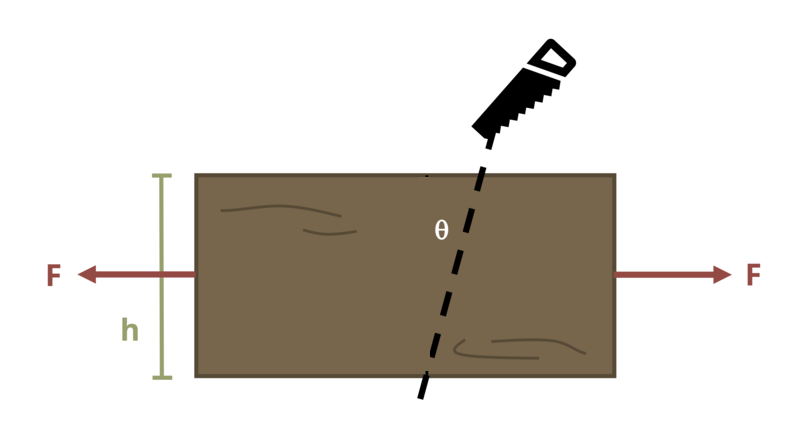
\includegraphics[keepaspectratio]{images/156.png}}
{[}Problem adapted from © Kurt Gramoll CC BY NC-SA 4.0{]}

\begin{Shaded}
\begin{Highlighting}[]
\NormalTok{\#| standalone: true}
\NormalTok{\#| viewerHeight: 600}
\NormalTok{\#| components: [viewer]}

\NormalTok{from shiny import App, render, ui, reactive}
\NormalTok{import random}
\NormalTok{import asyncio}
\NormalTok{import io}
\NormalTok{import math}
\NormalTok{import string}
\NormalTok{from datetime import datetime}
\NormalTok{from pathlib import Path}

\NormalTok{def generate\_random\_letters(length):}
\NormalTok{    \# Generate a random string of letters of specified length}
\NormalTok{    return \textquotesingle{}\textquotesingle{}.join(random.choice(string.ascii\_lowercase) for \_ in range(length))  }

\NormalTok{problem\_ID="156"}
\NormalTok{F=reactive.Value("\_\_")}
\NormalTok{h=reactive.Value("\_\_")}
\NormalTok{Θ=reactive.Value("\_\_")}

\NormalTok{attempts=["Timestamp,Attempt,Answer,Feedback\textbackslash{}n"]}

\NormalTok{app\_ui = ui.page\_fluid(}
\NormalTok{    \#ui.markdown("**Please enter your ID number from your instructor and click to generate your problem**"),}
\NormalTok{    \#ui.input\_text("ID","", placeholder="Enter ID Number Here"),}
\NormalTok{    \#ui.input\_action\_button("generate\_problem", "Generate Problem", class\_="btn{-}primary"),}
\NormalTok{    ui.markdown("**Problem Statement**"),}
\NormalTok{    ui.output\_ui("ui\_problem\_statement"),}
\NormalTok{    ui.input\_text("answer","Your Answer in units of psi", placeholder="Please enter your answer"),}
\NormalTok{    ui.input\_action\_button("submit", "Check Answer", class\_="btn{-}primary"),}
\NormalTok{    \#ui.download\_button("download", "Download File to Submit", class\_="btn{-}success"),}
\NormalTok{)}


\NormalTok{def server(input, output, session):}
\NormalTok{    \# Initialize a counter for attempts}
\NormalTok{    attempt\_counter = reactive.Value(0)}

\NormalTok{    @output}
\NormalTok{    @render.ui}
\NormalTok{    def ui\_problem\_statement():}
\NormalTok{        randomize\_vars()}
\NormalTok{        return[ui.markdown(f"A 2 inch thick board is cut and then glued back together along a line that is Θ = \{Θ()\} ° off the horizontal as shown. If height h = \{h()\} in. and F = \{F()\} lb, determine the normal stress along the cut line.")]}
    
\NormalTok{    \#@reactive.Effect}
\NormalTok{    \#@reactive.event(input.generate\_problem)}
\NormalTok{    def randomize\_vars():}
\NormalTok{        random.seed(101)}
\NormalTok{        F.set(random.randrange(2000, 6000, 100))}
\NormalTok{        h.set(random.randrange(50, 150, 1)/10)}
\NormalTok{        Θ.set(72)\#(random.randrange(10, 20, 1))}
        

\NormalTok{    @reactive.Effect}
\NormalTok{    @reactive.event(input.submit)}
\NormalTok{    def \_():}
\NormalTok{        attempt\_counter.set(attempt\_counter() + 1)  \# Increment the attempt counter on each submission.}
        
\NormalTok{        instr= (F()/(2*h()))*(math.sin(math.radians(Θ()))**2)}
\NormalTok{        if math.isclose(float(input.answer()), instr, rel\_tol=0.01):}
\NormalTok{            check = "*Correct*"}
\NormalTok{            correct\_indicator = "JL"}
\NormalTok{        else:}
\NormalTok{            check = "*Not Correct.*"}
\NormalTok{            correct\_indicator = "JG"}

\NormalTok{        \# Generate random parts for the encoded attempt.}
\NormalTok{        random\_start = generate\_random\_letters(4)}
\NormalTok{        random\_middle = generate\_random\_letters(4)}
\NormalTok{        random\_end = generate\_random\_letters(4)}
\NormalTok{        \#encoded\_attempt = f"\{random\_start\}\{problem\_ID\}{-}\{random\_middle\}\{attempt\_counter()\}\{correct\_indicator\}{-}\{random\_end\}\{input.ID()\}"}

\NormalTok{        \# Store the most recent encoded attempt in a reactive value so it persists across submissions}
\NormalTok{        \#session.encoded\_attempt = reactive.Value(encoded\_attempt)}

\NormalTok{        \# Append the attempt data to the attempts list without the encoded attempt}
\NormalTok{        attempts.append(f"\{datetime.now()\}, \{attempt\_counter()\}, \{input.answer()\}, \{check\}\textbackslash{}n")}

\NormalTok{        \# Show feedback to the user.}
\NormalTok{        feedback = ui.markdown(f"Your answer of \{input.answer()\} is \{check\}.")}
\NormalTok{        m = ui.modal(}
\NormalTok{            feedback,}
\NormalTok{            title="Feedback",}
\NormalTok{            easy\_close=True}
\NormalTok{        )}
\NormalTok{        ui.modal\_show(m)}

\NormalTok{    \#@render.download(filename=lambda: f"Problem\_Log{-}\{problem\_ID\}{-}\{input.ID()\}.csv")}
\NormalTok{    async def download():}
\NormalTok{        \# Start the CSV with the encoded attempt (without label)}
\NormalTok{        final\_encoded = session.encoded\_attempt() if session.encoded\_attempt is not None else "No attempts"}
\NormalTok{        yield f"\{final\_encoded\}\textbackslash{}n\textbackslash{}n"}
        
\NormalTok{        \# Write the header for the remaining CSV data once}
\NormalTok{        yield "Timestamp,Attempt,Answer,Feedback\textbackslash{}n"}
        
\NormalTok{        \# Write the attempts data, ensure that the header from the attempts list is not written again}
\NormalTok{        for attempt in attempts[1:]:  \# Skip the first element which is the header}
\NormalTok{            await asyncio.sleep(0.25)  \# This delay may not be necessary; adjust as needed}
\NormalTok{            yield attempt}


\NormalTok{\# App installation}
\NormalTok{app = App(app\_ui, server)}
\end{Highlighting}
\end{Shaded}

\part{Chapter 3 Problems}

\chapter*{Problem 3.1 - Normal
Strain}\label{problem-3.1---normal-strain}
\addcontentsline{toc}{chapter}{Problem 3.1 - Normal Strain}

\markboth{Problem 3.1 - Normal Strain}{Problem 3.1 - Normal Strain}

\pandocbounded{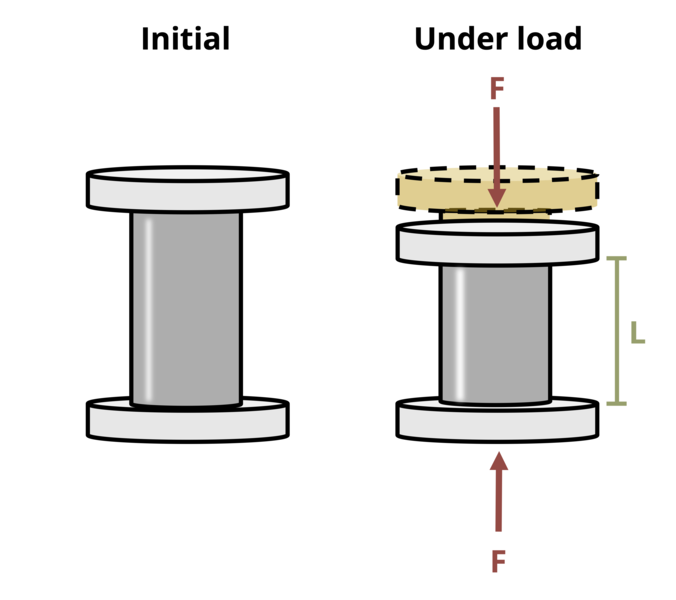
\includegraphics[keepaspectratio]{images/196.png}}
{[}Problem adapted from © Kurt Gramoll CC BY NC-SA 4.0{]}

\begin{Shaded}
\begin{Highlighting}[]
\NormalTok{\#| standalone: true}
\NormalTok{\#| viewerHeight: 600}
\NormalTok{\#| components: [viewer]}

\NormalTok{from shiny import App, render, ui, reactive}
\NormalTok{import random}
\NormalTok{import asyncio}
\NormalTok{import io}
\NormalTok{import math}
\NormalTok{import string}
\NormalTok{from datetime import datetime}
\NormalTok{from pathlib import Path}

\NormalTok{def generate\_random\_letters(length):}
\NormalTok{    \# Generate a random string of letters of specified length}
\NormalTok{    return \textquotesingle{}\textquotesingle{}.join(random.choice(string.ascii\_lowercase) for \_ in range(length))  }

\NormalTok{problem\_ID="196"}
\NormalTok{percent=reactive.Value("\_\_")}
\NormalTok{F=reactive.Value("\_\_")}
\NormalTok{L=reactive.Value("\_\_")}
  
\NormalTok{attempts=["Timestamp,Attempt,Answer,Feedback\textbackslash{}n"]}

\NormalTok{app\_ui = ui.page\_fluid(}
\NormalTok{    \#ui.markdown("**Please enter your ID number from your instructor and click to generate your problem**"),}
\NormalTok{    \#ui.input\_text("ID","", placeholder="Enter ID Number Here"),}
\NormalTok{    \#ui.input\_action\_button("generate\_problem", "Generate Problem", class\_="btn{-}primary"),}
\NormalTok{    ui.markdown("**Problem Statement**"),}
\NormalTok{    ui.output\_ui("ui\_problem\_statement"),}
\NormalTok{    ui.input\_text("answer","Your Answer", placeholder="Please enter your answer"),}
\NormalTok{    ui.input\_action\_button("submit", "Check Answer", class\_="btn{-}primary"),}
\NormalTok{    \#ui.download\_button("download", "Download File to Submit", class\_="btn{-}success"),}
\NormalTok{)}


\NormalTok{def server(input, output, session):}
\NormalTok{    \# Initialize a counter for attempts}
\NormalTok{    attempt\_counter = reactive.Value(0)}

\NormalTok{    @output}
\NormalTok{    @render.ui}
\NormalTok{    def ui\_problem\_statement():}
\NormalTok{        randomize\_vars()}
\NormalTok{        return[ui.markdown(f"A rubber cylinder experiences a \{percent()\}\% reduction in length ofter being exposed to a force F = \{F()\} lb. The cylinder has length L = \{L()\} in. after the load is applied. Determine the strain in the cylinder.")]}
    
\NormalTok{    \#@reactive.Effect}
\NormalTok{    \#@reactive.event(input.generate\_problem)}
\NormalTok{    def randomize\_vars():}
\NormalTok{        random.seed(101)}
\NormalTok{        percent.set(random.randrange(10,25,1))}
\NormalTok{        F.set(random.randrange(20,100,1))}
\NormalTok{        L.set(random.randrange(10,100,1)/10)}

\NormalTok{    @reactive.Effect}
\NormalTok{    @reactive.event(input.submit)}
\NormalTok{    def \_():}
\NormalTok{        attempt\_counter.set(attempt\_counter() + 1)  \# Increment the attempt counter on each submission.}
\NormalTok{        instr = {-}percent()/100}
        
\NormalTok{        if math.isclose(float(input.answer()), instr, rel\_tol=0.01):}
\NormalTok{            check = "*Correct*"}
\NormalTok{            correct\_indicator = "JL"}
\NormalTok{        else:}
\NormalTok{            check = "*Not Correct.*"}
\NormalTok{            correct\_indicator = "JG"}

\NormalTok{        \# Generate random parts for the encoded attempt.}
\NormalTok{        random\_start = generate\_random\_letters(4)}
\NormalTok{        random\_middle = generate\_random\_letters(4)}
\NormalTok{        random\_end = generate\_random\_letters(4)}
\NormalTok{        \#encoded\_attempt = f"\{random\_start\}\{problem\_ID\}{-}\{random\_middle\}\{attempt\_counter()\}\{correct\_indicator\}{-}\{random\_end\}\{input.ID()\}"}

\NormalTok{        \# Store the most recent encoded attempt in a reactive value so it persists across submissions}
\NormalTok{        \#session.encoded\_attempt = reactive.Value(encoded\_attempt)}

\NormalTok{        \# Append the attempt data to the attempts list without the encoded attempt}
\NormalTok{        attempts.append(f"\{datetime.now()\}, \{attempt\_counter()\}, \{input.answer()\}, \{check\}\textbackslash{}n")}

\NormalTok{        \# Show feedback to the user.}
\NormalTok{        feedback = ui.markdown(f"Your answer of \{input.answer()\} is \{check\}.")}
\NormalTok{        m = ui.modal(}
\NormalTok{            feedback,}
\NormalTok{            title="Feedback",}
\NormalTok{            easy\_close=True}
\NormalTok{        )}
\NormalTok{        ui.modal\_show(m)}

\NormalTok{    \#@render.download(filename=lambda: f"Problem\_Log{-}\{problem\_ID\}{-}\{input.ID()\}.csv")}
\NormalTok{    async def download():}
\NormalTok{        \# Start the CSV with the encoded attempt (without label)}
\NormalTok{        final\_encoded = session.encoded\_attempt() if session.encoded\_attempt is not None else "No attempts"}
\NormalTok{        yield f"\{final\_encoded\}\textbackslash{}n\textbackslash{}n"}
        
\NormalTok{        \# Write the header for the remaining CSV data once}
\NormalTok{        yield "Timestamp,Attempt,Answer,Feedback\textbackslash{}n"}
        
\NormalTok{        \# Write the attempts data, ensure that the header from the attempts list is not written again}
\NormalTok{        for attempt in attempts[1:]:  \# Skip the first element which is the header}
\NormalTok{            await asyncio.sleep(0.25)  \# This delay may not be necessary; adjust as needed}
\NormalTok{            yield attempt}

\NormalTok{\# App installation}
\NormalTok{app = App(app\_ui, server)}
\end{Highlighting}
\end{Shaded}

\chapter*{Problem 3.2 - Normal
Strain}\label{problem-3.2---normal-strain}
\addcontentsline{toc}{chapter}{Problem 3.2 - Normal Strain}

\markboth{Problem 3.2 - Normal Strain}{Problem 3.2 - Normal Strain}

\begin{figure}[H]

{\centering 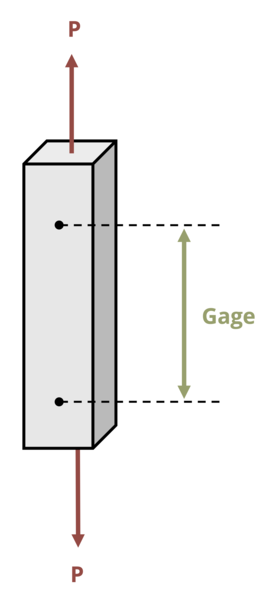
\includegraphics[width=1.5625in,height=\textheight,keepaspectratio]{images/650.png}

}

\caption{Figure 1: A rectangular prism is subjected to a tension test.}

\end{figure}%

{[}Problem adapted from © Chris Galitz CC BY NC-SA 4.0{]}

\begin{Shaded}
\begin{Highlighting}[]
\NormalTok{\#| standalone: true}
\NormalTok{\#| viewerHeight: 600}
\NormalTok{\#| components: [viewer]}

\NormalTok{from shiny import App, render, ui, reactive}
\NormalTok{import random}
\NormalTok{import asyncio}
\NormalTok{import io}
\NormalTok{import math}
\NormalTok{import string}
\NormalTok{from datetime import datetime}
\NormalTok{from pathlib import Path}

\NormalTok{def generate\_random\_letters(length):}
\NormalTok{    \# Generate a random string of letters of specified length}
\NormalTok{    return \textquotesingle{}\textquotesingle{}.join(random.choice(string.ascii\_lowercase) for \_ in range(length))  }

\NormalTok{problem\_ID="650"}
\NormalTok{L=reactive.Value("\_\_")}
\NormalTok{Lp=reactive.Value("\_\_")}

  
\NormalTok{attempts=["Timestamp,Attempt,Answer,Feedback\textbackslash{}n"]}

\NormalTok{app\_ui = ui.page\_fluid(}
\NormalTok{    \#ui.markdown("**Please enter your ID number from your instructor and click to generate your problem**"),}
\NormalTok{    \#ui.input\_text("ID","", placeholder="Enter ID Number Here"),}
\NormalTok{    \#ui.input\_action\_button("generate\_problem", "Generate Problem", class\_="btn{-}primary"),}
\NormalTok{    ui.markdown("**Problem Statement**"),}
\NormalTok{    ui.output\_ui("ui\_problem\_statement"),}
\NormalTok{    ui.input\_text("answer","Your Answer in units of mm/mm", placeholder="Please enter your answer"),}
\NormalTok{    ui.input\_action\_button("submit", "Check Answer", class\_="btn{-}primary"),}
\NormalTok{    \#ui.download\_button("download", "Download File to Submit", class\_="btn{-}success"),}
\NormalTok{)}


\NormalTok{def server(input, output, session):}
\NormalTok{    \# Initialize a counter for attempts}
\NormalTok{    attempt\_counter = reactive.Value(0)}

\NormalTok{    @output}
\NormalTok{    @render.ui}
\NormalTok{    def ui\_problem\_statement():}
\NormalTok{        randomize\_vars()}
\NormalTok{        return[ui.markdown(f"During a tension test of a rectangular prism, the original gage length L = \{L()\} mm is increased to L\textquotesingle{} = \{Lp()\} mm. determine the normal strain, ε, in the prism.")]}
    
\NormalTok{    \#@reactive.Effect}
\NormalTok{    \#@reactive.event(input.generate\_problem)}
\NormalTok{    def randomize\_vars():}
\NormalTok{        random.seed(101)}
\NormalTok{        L.set(random.randrange(100, 400, 1))}
\NormalTok{        Lp.set(L()+random.randrange(100, 300, 1)/100)}
        
\NormalTok{    @reactive.Effect}
\NormalTok{    @reactive.event(input.submit)}
\NormalTok{    def \_():}
\NormalTok{        attempt\_counter.set(attempt\_counter() + 1)  \# Increment the attempt counter on each submission.}
\NormalTok{        instr= (Lp(){-}L())/L()}
\NormalTok{        if math.isclose(float(input.answer()), instr, rel\_tol=0.01):}
\NormalTok{            check = "*Correct*"}
\NormalTok{            correct\_indicator = "JL"}
\NormalTok{        else:}
\NormalTok{            check = "*Not Correct.*"}
\NormalTok{            correct\_indicator = "JG"}

\NormalTok{        \# Generate random parts for the encoded attempt.}
\NormalTok{        random\_start = generate\_random\_letters(4)}
\NormalTok{        random\_middle = generate\_random\_letters(4)}
\NormalTok{        random\_end = generate\_random\_letters(4)}
\NormalTok{        \#encoded\_attempt = f"\{random\_start\}\{problem\_ID\}{-}\{random\_middle\}\{attempt\_counter()\}\{correct\_indicator\}{-}\{random\_end\}\{input.ID()\}"}

\NormalTok{        \# Store the most recent encoded attempt in a reactive value so it persists across submissions}
\NormalTok{        \#session.encoded\_attempt = reactive.Value(encoded\_attempt)}

\NormalTok{        \# Append the attempt data to the attempts list without the encoded attempt}
\NormalTok{        attempts.append(f"\{datetime.now()\}, \{attempt\_counter()\}, \{input.answer()\}, \{check\}\textbackslash{}n")}

\NormalTok{        \# Show feedback to the user.}
\NormalTok{        feedback = ui.markdown(f"Your answer of \{input.answer()\} is \{check\}.")}
\NormalTok{        m = ui.modal(}
\NormalTok{            feedback,}
\NormalTok{            title="Feedback",}
\NormalTok{            easy\_close=True}
\NormalTok{        )}
\NormalTok{        ui.modal\_show(m)}

\NormalTok{    \#@render.download(filename=lambda: f"Problem\_Log{-}\{problem\_ID\}{-}\{input.ID()\}.csv")}
\NormalTok{    async def download():}
\NormalTok{        \# Start the CSV with the encoded attempt (without label)}
\NormalTok{        final\_encoded = session.encoded\_attempt() if session.encoded\_attempt is not None else "No attempts"}
\NormalTok{        yield f"\{final\_encoded\}\textbackslash{}n\textbackslash{}n"}
        
\NormalTok{        \# Write the header for the remaining CSV data once}
\NormalTok{        yield "Timestamp,Attempt,Answer,Feedback\textbackslash{}n"}
        
\NormalTok{        \# Write the attempts data, ensure that the header from the attempts list is not written again}
\NormalTok{        for attempt in attempts[1:]:  \# Skip the first element which is the header}
\NormalTok{            await asyncio.sleep(0.25)  \# This delay may not be necessary; adjust as needed}
\NormalTok{            yield attempt}


\NormalTok{\# App installation}
\NormalTok{app = App(app\_ui, server)}
\end{Highlighting}
\end{Shaded}

\chapter*{Problem 3.3 - Normal
Strain}\label{problem-3.3---normal-strain}
\addcontentsline{toc}{chapter}{Problem 3.3 - Normal Strain}

\markboth{Problem 3.3 - Normal Strain}{Problem 3.3 - Normal Strain}

{[}Problem adapted from © Chris Galitz CC BY NC-SA 4.0{]}

\begin{Shaded}
\begin{Highlighting}[]
\NormalTok{\#| standalone: true}
\NormalTok{\#| viewerHeight: 600}
\NormalTok{\#| components: [viewer]}

\NormalTok{from shiny import App, render, ui, reactive}
\NormalTok{import random}
\NormalTok{import asyncio}
\NormalTok{import io}
\NormalTok{import math}
\NormalTok{import string}
\NormalTok{from datetime import datetime}
\NormalTok{from pathlib import Path}

\NormalTok{def generate\_random\_letters(length):}
\NormalTok{    \# Generate a random string of letters of specified length}
\NormalTok{    return \textquotesingle{}\textquotesingle{}.join(random.choice(string.ascii\_lowercase) for \_ in range(length))  }

\NormalTok{problem\_ID="139"}
\NormalTok{L1=reactive.Value("\_\_")}
\NormalTok{L2=reactive.Value("\_\_")}
\NormalTok{FA=reactive.Value("\_\_")}
\NormalTok{FB=reactive.Value("\_\_")}
\NormalTok{E = 30*10**6}
  
\NormalTok{attempts=["Timestamp,Attempt,Answer,Feedback\textbackslash{}n"]}

\NormalTok{app\_ui = ui.page\_fluid(}
\NormalTok{    \#ui.markdown("**Please enter your ID number from your instructor and click to generate your problem**"),}
\NormalTok{    \#ui.input\_text("ID","", placeholder="Enter ID Number Here"),}
\NormalTok{    \#ui.input\_action\_button("generate\_problem", "Generate Problem", class\_="btn{-}primary"),}
\NormalTok{    ui.markdown("**Problem Statement**"),}
\NormalTok{    ui.output\_ui("ui\_problem\_statement"),}
\NormalTok{    ui.input\_text("answer","Your Answer in units of inches", placeholder="Please enter your answer"),}
\NormalTok{    ui.input\_action\_button("submit", "Check Answer", class\_="btn{-}primary"),}
\NormalTok{    \#ui.download\_button("download", "Download File to Submit", class\_="btn{-}success"),}
\NormalTok{)}


\NormalTok{def server(input, output, session):}
\NormalTok{    \# Initialize a counter for attempts}
\NormalTok{    attempt\_counter = reactive.Value(0)}

\NormalTok{    @output}
\NormalTok{    @render.ui}
\NormalTok{    def ui\_problem\_statement():}
\NormalTok{        randomize\_vars()}
\NormalTok{        return[ui.markdown(f"Two cylinders are stacked on top of one another and two forces are applied at the top surface and at the joint between the cylinders as shown. If L\textless{}sub\textgreater{}1\textless{}/sub\textgreater{} = \{L1()\} in., L\textless{}sub\textgreater{}2\textless{}/sub\textgreater{} = \{L2()\} in., F\textless{}sub\textgreater{}A\textless{}/sub\textgreater{} = \{FA()\} lb, and F\textless{}sub\textgreater{}B\textless{}/sub\textgreater{} = \{FB()\} lb, find the total deflection in the stack of cylinders. Assume E = 30 x 10\textless{}sup\textgreater{}6\textless{}/sup\textgreater{} psi for both cylinders. ")]}
    
\NormalTok{    \#@reactive.Effect}
\NormalTok{    \#@reactive.event(input.generate\_problem)}
\NormalTok{    def randomize\_vars():}
\NormalTok{        random.seed(101)}
\NormalTok{        FA.set(random.randrange(300, 700, 10))}
\NormalTok{        FB.set(random.randrange(100, 300, 10))}
\NormalTok{        L1.set(random.randrange(2, 7, 1))}
\NormalTok{        L2.set(L1() * 1.3)}
        

\NormalTok{    @reactive.Effect}
\NormalTok{    @reactive.event(input.submit)}
\NormalTok{    def \_():}
\NormalTok{        attempt\_counter.set(attempt\_counter() + 1)  \# Increment the attempt counter on each submission.}
    
\NormalTok{        instr= (FA()*L1())/((math.pi*(5/2)**2)*E) + (FB()*L2())/((math.pi*(3/2)**2)*E)}
\NormalTok{        if math.isclose(float(input.answer()), instr, rel\_tol=0.01):}
\NormalTok{            check = "*Correct*"}
\NormalTok{            correct\_indicator = "JL"}
\NormalTok{        else:}
\NormalTok{            check = "*Not Correct.*"}
\NormalTok{            correct\_indicator = "JG"}

\NormalTok{        \# Generate random parts for the encoded attempt.}
\NormalTok{        random\_start = generate\_random\_letters(4)}
\NormalTok{        random\_middle = generate\_random\_letters(4)}
\NormalTok{        random\_end = generate\_random\_letters(4)}
\NormalTok{        \#encoded\_attempt = f"\{random\_start\}\{problem\_ID\}{-}\{random\_middle\}\{attempt\_counter()\}\{correct\_indicator\}{-}\{random\_end\}\{input.ID()\}"}

\NormalTok{        \# Store the most recent encoded attempt in a reactive value so it persists across submissions}
\NormalTok{        \#session.encoded\_attempt = reactive.Value(encoded\_attempt)}

\NormalTok{        \# Append the attempt data to the attempts list without the encoded attempt}
\NormalTok{        attempts.append(f"\{datetime.now()\}, \{attempt\_counter()\}, \{input.answer()\}, \{check\}\textbackslash{}n")}

\NormalTok{        \# Show feedback to the user.}
\NormalTok{        feedback = ui.markdown(f"Your answer of \{input.answer()\} is \{check\}.")}
\NormalTok{        m = ui.modal(}
\NormalTok{            feedback,}
\NormalTok{            title="Feedback",}
\NormalTok{            easy\_close=True}
\NormalTok{        )}
\NormalTok{        ui.modal\_show(m)}

\NormalTok{    \#@render.download(filename=lambda: f"Problem\_Log{-}\{problem\_ID\}{-}\{input.ID()\}.csv")}
\NormalTok{    async def download():}
\NormalTok{        \# Start the CSV with the encoded attempt (without label)}
\NormalTok{        final\_encoded = session.encoded\_attempt() if session.encoded\_attempt is not None else "No attempts"}
\NormalTok{        yield f"\{final\_encoded\}\textbackslash{}n\textbackslash{}n"}
        
\NormalTok{        \# Write the header for the remaining CSV data once}
\NormalTok{        yield "Timestamp,Attempt,Answer,Feedback\textbackslash{}n"}
        
\NormalTok{        \# Write the attempts data, ensure that the header from the attempts list is not written again}
\NormalTok{        for attempt in attempts[1:]:  \# Skip the first element which is the header}
\NormalTok{            await asyncio.sleep(0.25)  \# This delay may not be necessary; adjust as needed}
\NormalTok{            yield attempt}


\NormalTok{\# App installation}
\NormalTok{app = App(app\_ui, server)}
\end{Highlighting}
\end{Shaded}

\chapter*{Problem 3.7 - Shear Strain}\label{problem-3.7---shear-strain}
\addcontentsline{toc}{chapter}{Problem 3.7 - Shear Strain}

\markboth{Problem 3.7 - Shear Strain}{Problem 3.7 - Shear Strain}

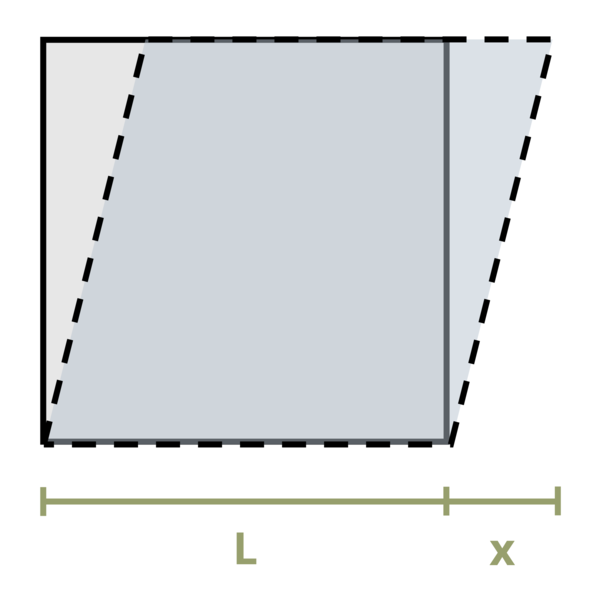
\includegraphics[width=3.125in,height=\textheight,keepaspectratio]{images/652.png}
{[}Problem adapted from © Chris Galitz CC BY NC-SA 4.0{]}

\begin{Shaded}
\begin{Highlighting}[]
\NormalTok{\#| standalone: true}
\NormalTok{\#| viewerHeight: 600}
\NormalTok{\#| components: [viewer]}

\NormalTok{from shiny import App, render, ui, reactive}
\NormalTok{import random}
\NormalTok{import asyncio}
\NormalTok{import io}
\NormalTok{import math}
\NormalTok{import string}
\NormalTok{from datetime import datetime}
\NormalTok{from pathlib import Path}

\NormalTok{def generate\_random\_letters(length):}
\NormalTok{    \# Generate a random string of letters of specified length}
\NormalTok{    return \textquotesingle{}\textquotesingle{}.join(random.choice(string.ascii\_lowercase) for \_ in range(length))  }

\NormalTok{problem\_ID="652"}
\NormalTok{L=reactive.Value("\_\_")}
\NormalTok{x=reactive.Value("\_\_")}

  
\NormalTok{attempts=["Timestamp,Attempt,Answer,Feedback\textbackslash{}n"]}

\NormalTok{app\_ui = ui.page\_fluid(}
\NormalTok{    \#ui.markdown("**Please enter your ID number from your instructor and click to generate your problem**"),}
\NormalTok{    \#ui.input\_text("ID","", placeholder="Enter ID Number Here"),}
\NormalTok{    \#ui.input\_action\_button("generate\_problem", "Generate Problem", class\_="btn{-}primary"),}
\NormalTok{    ui.markdown("**Problem Statement**"),}
\NormalTok{    ui.output\_ui("ui\_problem\_statement"),}
\NormalTok{    ui.input\_text("answer","Your Answer in units of radians", placeholder="Please enter your answer"),}
\NormalTok{    ui.input\_action\_button("submit", "Check Answer", class\_="btn{-}primary"),}
\NormalTok{    \#ui.download\_button("download", "Download File to Submit", class\_="btn{-}success"),}
\NormalTok{)}


\NormalTok{def server(input, output, session):}
\NormalTok{    \# Initialize a counter for attempts}
\NormalTok{    attempt\_counter = reactive.Value(0)}

\NormalTok{    @output}
\NormalTok{    @render.ui}
\NormalTok{    def ui\_problem\_statement():}
\NormalTok{        randomize\_vars()}
\NormalTok{        return[ui.markdown(f"A square plate is deformed due to shear with the new shape shown. If length L = \{L()\} mm and x = \{x()\} mm, determine the shear strain at the bottom left corner.")]}
    
\NormalTok{    \#@reactive.Effect}
\NormalTok{    \#@reactive.event(input.generate\_problem)}
\NormalTok{    def randomize\_vars():}
\NormalTok{        random.seed(101)}
\NormalTok{        L.set(random.randrange(200, 500, 10))}
\NormalTok{        x.set(random.randrange(20, 50, 1))}
        
\NormalTok{    @reactive.Effect}
\NormalTok{    @reactive.event(input.submit)}
\NormalTok{    def \_():}
\NormalTok{        attempt\_counter.set(attempt\_counter() + 1)  \# Increment the attempt counter on each submission.}
\NormalTok{        instr= math.atan(x()/L())}
\NormalTok{        if math.isclose(float(input.answer()), instr, rel\_tol=0.01):}
\NormalTok{            check = "*Correct*"}
\NormalTok{            correct\_indicator = "JL"}
\NormalTok{        else:}
\NormalTok{            check = "*Not Correct.*"}
\NormalTok{            correct\_indicator = "JG"}

\NormalTok{        \# Generate random parts for the encoded attempt.}
\NormalTok{        random\_start = generate\_random\_letters(4)}
\NormalTok{        random\_middle = generate\_random\_letters(4)}
\NormalTok{        random\_end = generate\_random\_letters(4)}
\NormalTok{        \#encoded\_attempt = f"\{random\_start\}\{problem\_ID\}{-}\{random\_middle\}\{attempt\_counter()\}\{correct\_indicator\}{-}\{random\_end\}\{input.ID()\}"}

\NormalTok{        \# Store the most recent encoded attempt in a reactive value so it persists across submissions}
\NormalTok{        \#session.encoded\_attempt = reactive.Value(encoded\_attempt)}

\NormalTok{        \# Append the attempt data to the attempts list without the encoded attempt}
\NormalTok{        attempts.append(f"\{datetime.now()\}, \{attempt\_counter()\}, \{input.answer()\}, \{check\}\textbackslash{}n")}

\NormalTok{        \# Show feedback to the user.}
\NormalTok{        feedback = ui.markdown(f"Your answer of \{input.answer()\} is \{check\}.")}
\NormalTok{        m = ui.modal(}
\NormalTok{            feedback,}
\NormalTok{            title="Feedback",}
\NormalTok{            easy\_close=True}
\NormalTok{        )}
\NormalTok{        ui.modal\_show(m)}

\NormalTok{    \#@render.download(filename=lambda: f"Problem\_Log{-}\{problem\_ID\}{-}\{input.ID()\}.csv")}
\NormalTok{    async def download():}
\NormalTok{        \# Start the CSV with the encoded attempt (without label)}
\NormalTok{        final\_encoded = session.encoded\_attempt() if session.encoded\_attempt is not None else "No attempts"}
\NormalTok{        yield f"\{final\_encoded\}\textbackslash{}n\textbackslash{}n"}
        
\NormalTok{        \# Write the header for the remaining CSV data once}
\NormalTok{        yield "Timestamp,Attempt,Answer,Feedback\textbackslash{}n"}
        
\NormalTok{        \# Write the attempts data, ensure that the header from the attempts list is not written again}
\NormalTok{        for attempt in attempts[1:]:  \# Skip the first element which is the header}
\NormalTok{            await asyncio.sleep(0.25)  \# This delay may not be necessary; adjust as needed}
\NormalTok{            yield attempt}


\NormalTok{\# App installation}
\NormalTok{app = App(app\_ui, server)}
\end{Highlighting}
\end{Shaded}

\chapter*{Problem 3.8 - Shear Strain}\label{problem-3.8---shear-strain}
\addcontentsline{toc}{chapter}{Problem 3.8 - Shear Strain}

\markboth{Problem 3.8 - Shear Strain}{Problem 3.8 - Shear Strain}

\pandocbounded{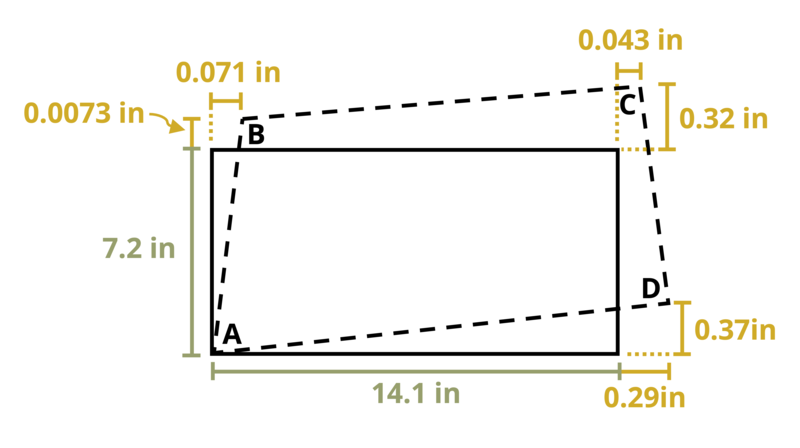
\includegraphics[keepaspectratio]{images/653.png}}
{[}Problem adapted from © Chris Galitz CC BY NC-SA 4.0{]}

\begin{Shaded}
\begin{Highlighting}[]
\NormalTok{\#| standalone: true}
\NormalTok{\#| viewerHeight: 600}
\NormalTok{\#| components: [viewer]}

\NormalTok{from shiny import App, render, ui, reactive}
\NormalTok{import random}
\NormalTok{import asyncio}
\NormalTok{import io}
\NormalTok{import math}
\NormalTok{import string}
\NormalTok{from datetime import datetime}
\NormalTok{from pathlib import Path}

\NormalTok{def generate\_random\_letters(length):}
\NormalTok{    \# Generate a random string of letters of specified length}
\NormalTok{    return \textquotesingle{}\textquotesingle{}.join(random.choice(string.ascii\_lowercase) for \_ in range(length))  }

\NormalTok{problem\_ID="653"}
\NormalTok{h=reactive.Value("\_\_")}
\NormalTok{L=reactive.Value("\_\_")}
  
\NormalTok{attempts=["Timestamp,Attempt,Answer,Feedback\textbackslash{}n"]}

\NormalTok{app\_ui = ui.page\_fluid(}
\NormalTok{    \#ui.markdown("**Please enter your ID number from your instructor and click to generate your problem**"),}
\NormalTok{    \#ui.input\_text("ID","", placeholder="Enter ID Number Here"),}
\NormalTok{    \#ui.input\_action\_button("generate\_problem", "Generate Problem", class\_="btn{-}primary"),}
\NormalTok{    ui.markdown("**Problem Statement**"),}
\NormalTok{    ui.output\_ui("ui\_problem\_statement"),}
\NormalTok{    ui.input\_text("answer","Your Answer in units of radians", placeholder="Please enter your answer"),}
\NormalTok{    ui.input\_action\_button("submit", "Check Answer", class\_="btn{-}primary"),}
\NormalTok{    \#ui.download\_button("download", "Download File to Submit", class\_="btn{-}success"),}
\NormalTok{)}

\NormalTok{def server(input, output, session):}
\NormalTok{    \# Initialize a counter for attempts}
\NormalTok{    attempt\_counter = reactive.Value(0)}

\NormalTok{    @output}
\NormalTok{    @render.ui}
\NormalTok{    def ui\_problem\_statement():}
\NormalTok{        randomize\_vars()}
\NormalTok{        return[ui.markdown(f"A rectangular plate of dimensions L = \{L()\} in. and h = \{h()\} in. is deformed to the new shape shown. Determine the shear strain at corner A."}
\NormalTok{            )}
\NormalTok{        ]}

\NormalTok{    \#@reactive.Effect}
\NormalTok{    \#@reactive.event(input.generate\_problem)}
\NormalTok{    def randomize\_vars():}
\NormalTok{        random.seed(101)}
\NormalTok{        h.set(7.2)\#(random.randrange(50,100,1)/10)}
\NormalTok{        L.set(14.1)\#(h()+random.randrange(50,100,1)/10)}

\NormalTok{    @reactive.Effect}
\NormalTok{    @reactive.event(input.submit)}
\NormalTok{    def \_():}
\NormalTok{        attempt\_counter.set(}
\NormalTok{            attempt\_counter() + 1}
\NormalTok{        )  \# Increment the attempt counter on each submission.}

\NormalTok{        \# Calculate the instructor\textquotesingle{}s answer and determine if the user\textquotesingle{}s answer is correct.}
\NormalTok{        alpha2 = 0.071/(h() + 0.0073)}
\NormalTok{        alpha3 = 0.37/(L() + 0.29)}
\NormalTok{        instr = alpha2 + alpha3}
\NormalTok{        if math.isclose(float(input.answer()), instr, rel\_tol=0.01):}
\NormalTok{            check = "*Correct*"}
\NormalTok{            correct\_indicator = "JL"}
\NormalTok{        else:}
\NormalTok{            check = "*Not Correct.*"}
\NormalTok{            correct\_indicator = "JG"}

\NormalTok{        \# Generate random parts for the encoded attempt.}
\NormalTok{        random\_start = generate\_random\_letters(4)}
\NormalTok{        random\_middle = generate\_random\_letters(4)}
\NormalTok{        random\_end = generate\_random\_letters(4)}
\NormalTok{        \#encoded\_attempt = f"\{random\_start\}\{problem\_ID\}{-}\{random\_middle\}\{attempt\_counter()\}\{correct\_indicator\}{-}\{random\_end\}\{input.ID()\}"}

\NormalTok{        \# Store the most recent encoded attempt in a reactive value so it persists across submissions}
\NormalTok{        \#session.encoded\_attempt = reactive.Value(encoded\_attempt)}

\NormalTok{        \# Append the attempt data to the attempts list without the encoded attempt}
\NormalTok{        attempts.append(f"\{datetime.now()\}, \{attempt\_counter()\}, \{input.answer()\}, \{check\}\textbackslash{}n")}

\NormalTok{        \# Show feedback to the user.}
\NormalTok{        feedback = ui.markdown(f"Your answer of \{input.answer()\} is \{check\}.")}
\NormalTok{        m = ui.modal(}
\NormalTok{            feedback,}
\NormalTok{            title="Feedback",}
\NormalTok{            easy\_close=True}
\NormalTok{        )}
\NormalTok{        ui.modal\_show(m)}

\NormalTok{    \#@render.download(filename=lambda: f"Problem\_Log{-}\{problem\_ID\}{-}\{input.ID()\}.csv")}
\NormalTok{    async def download():}
\NormalTok{        \# Start the CSV with the encoded attempt (without label)}
\NormalTok{        final\_encoded = session.encoded\_attempt() if session.encoded\_attempt is not None else "No attempts"}
\NormalTok{        yield f"\{final\_encoded\}\textbackslash{}n\textbackslash{}n"}
        
\NormalTok{        \# Write the header for the remaining CSV data once}
\NormalTok{        yield "Timestamp,Attempt,Answer,Feedback\textbackslash{}n"}
        
\NormalTok{        \# Write the attempts data, ensure that the header from the attempts list is not written again}
\NormalTok{        for attempt in attempts[1:]:  \# Skip the first element which is the header}
\NormalTok{            await asyncio.sleep(0.25)  \# This delay may not be necessary; adjust as needed}
\NormalTok{            yield attempt}

\NormalTok{\# App installation}
\NormalTok{app = App(app\_ui, server)}
\end{Highlighting}
\end{Shaded}

\chapter*{Problem 3.9 - Shear Strain}\label{problem-3.9---shear-strain}
\addcontentsline{toc}{chapter}{Problem 3.9 - Shear Strain}

\markboth{Problem 3.9 - Shear Strain}{Problem 3.9 - Shear Strain}

\pandocbounded{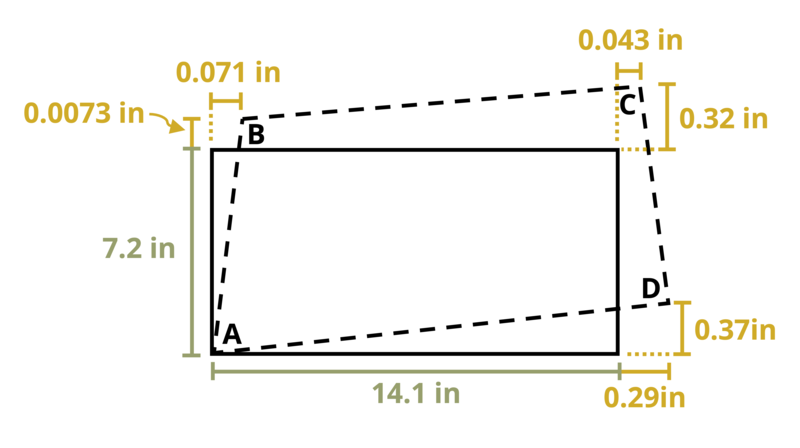
\includegraphics[keepaspectratio]{images/653.png}}
{[}Problem adapted from © Chris Galitz CC BY NC-SA 4.0{]}

\begin{Shaded}
\begin{Highlighting}[]
\NormalTok{\#| standalone: true}
\NormalTok{\#| viewerHeight: 600}
\NormalTok{\#| components: [viewer]}

\NormalTok{from shiny import App, render, ui, reactive}
\NormalTok{import random}
\NormalTok{import asyncio}
\NormalTok{import io}
\NormalTok{import math}
\NormalTok{import string}
\NormalTok{from datetime import datetime}
\NormalTok{from pathlib import Path}

\NormalTok{def generate\_random\_letters(length):}
\NormalTok{    \# Generate a random string of letters of specified length}
\NormalTok{    return \textquotesingle{}\textquotesingle{}.join(random.choice(string.ascii\_lowercase) for \_ in range(length))  }

\NormalTok{problem\_ID="654"}
\NormalTok{t=reactive.Value("\_\_")}
\NormalTok{x=reactive.Value("\_\_")}
  
\NormalTok{attempts=["Timestamp,Attempt,Answer,Feedback\textbackslash{}n"]}

\NormalTok{app\_ui = ui.page\_fluid(}
\NormalTok{    \#ui.markdown("**Please enter your ID number from your instructor and click to generate your problem**"),}
\NormalTok{    \#ui.input\_text("ID","", placeholder="Enter ID Number Here"),}
\NormalTok{    \#ui.input\_action\_button("generate\_problem", "Generate Problem", class\_="btn{-}primary"),}
\NormalTok{    ui.markdown("**Problem Statement**"),}
\NormalTok{    ui.output\_ui("ui\_problem\_statement"),}
\NormalTok{    ui.input\_text("answer","Your Answer in units of radians", placeholder="Please enter your answer"),}
\NormalTok{    ui.input\_action\_button("submit", "Check Answer", class\_="btn{-}primary"),}
\NormalTok{    \#ui.download\_button("download", "Download File to Submit", class\_="btn{-}success"),}
\NormalTok{)}

\NormalTok{def server(input, output, session):}
\NormalTok{    \# Initialize a counter for attempts}
\NormalTok{    attempt\_counter = reactive.Value(0)}

\NormalTok{    @output}
\NormalTok{    @render.ui}
\NormalTok{    def ui\_problem\_statement():}
\NormalTok{        randomize\_vars()}
\NormalTok{        return[ui.markdown(f"Two plates are connected by a neoprense pad of thickness t = \{t()\} mm that is bonded to each plate. The top plate shifts to the right by x = \{x()\} mm. It is observed that the edge of the pad forms symmetric circular arcs rather than a straight line. Determine the maximum strain in the neoprene."}
\NormalTok{            )}
\NormalTok{        ]}

\NormalTok{    \#@reactive.Effect}
\NormalTok{    \#@reactive.event(input.generate\_problem)}
\NormalTok{    def randomize\_vars():}
\NormalTok{        random.seed(101)}
\NormalTok{        t.set(random.randrange(10,30,1))}
\NormalTok{        x.set(random.randrange(10,30,1)/10)}

\NormalTok{    @reactive.Effect}
\NormalTok{    @reactive.event(input.submit)}
\NormalTok{    def \_():}
\NormalTok{        attempt\_counter.set(}
\NormalTok{            attempt\_counter() + 1}
\NormalTok{        )  \# Increment the attempt counter on each submission.}

\NormalTok{        \# Calculate the instructor\textquotesingle{}s answer and determine if the user\textquotesingle{}s answer is correct.}
\NormalTok{        y = (t()**2/4{-}x()**2/4)/x()}
\NormalTok{        r = y+x()/2}
\NormalTok{        theta = math.acos(x()/r)}
\NormalTok{        instr = math.pi/2{-}theta}
\NormalTok{        if math.isclose(float(input.answer()), instr, rel\_tol=0.01):}
\NormalTok{            check = "*Correct*"}
\NormalTok{            correct\_indicator = "JL"}
\NormalTok{        else:}
\NormalTok{            check = "*Not Correct.*"}
\NormalTok{            correct\_indicator = "JG"}

\NormalTok{        \# Generate random parts for the encoded attempt.}
\NormalTok{        random\_start = generate\_random\_letters(4)}
\NormalTok{        random\_middle = generate\_random\_letters(4)}
\NormalTok{        random\_end = generate\_random\_letters(4)}
\NormalTok{        \#encoded\_attempt = f"\{random\_start\}\{problem\_ID\}{-}\{random\_middle\}\{attempt\_counter()\}\{correct\_indicator\}{-}\{random\_end\}\{input.ID()\}"}

\NormalTok{        \# Store the most recent encoded attempt in a reactive value so it persists across submissions}
\NormalTok{        \#session.encoded\_attempt = reactive.Value(encoded\_attempt)}

\NormalTok{        \# Append the attempt data to the attempts list without the encoded attempt}
\NormalTok{        attempts.append(f"\{datetime.now()\}, \{attempt\_counter()\}, \{input.answer()\}, \{check\}\textbackslash{}n")}

\NormalTok{        \# Show feedback to the user.}
\NormalTok{        feedback = ui.markdown(f"Your answer of \{input.answer()\} is \{check\}.")}
\NormalTok{        m = ui.modal(}
\NormalTok{            feedback,}
\NormalTok{            title="Feedback",}
\NormalTok{            easy\_close=True}
\NormalTok{        )}
\NormalTok{        ui.modal\_show(m)}

\NormalTok{    \#@render.download(filename=lambda: f"Problem\_Log{-}\{problem\_ID\}{-}\{input.ID()\}.csv")}
\NormalTok{    async def download():}
\NormalTok{        \# Start the CSV with the encoded attempt (without label)}
\NormalTok{        final\_encoded = session.encoded\_attempt() if session.encoded\_attempt is not None else "No attempts"}
\NormalTok{        yield f"\{final\_encoded\}\textbackslash{}n\textbackslash{}n"}
        
\NormalTok{        \# Write the header for the remaining CSV data once}
\NormalTok{        yield "Timestamp,Attempt,Answer,Feedback\textbackslash{}n"}
        
\NormalTok{        \# Write the attempts data, ensure that the header from the attempts list is not written again}
\NormalTok{        for attempt in attempts[1:]:  \# Skip the first element which is the header}
\NormalTok{            await asyncio.sleep(0.25)  \# This delay may not be necessary; adjust as needed}
\NormalTok{            yield attempt}

\NormalTok{\# App installation}
\NormalTok{app = App(app\_ui, server)}
\end{Highlighting}
\end{Shaded}

\chapter*{Problem 3.10 - Shear
Strain}\label{problem-3.10---shear-strain}
\addcontentsline{toc}{chapter}{Problem 3.10 - Shear Strain}

\markboth{Problem 3.10 - Shear Strain}{Problem 3.10 - Shear Strain}

\pandocbounded{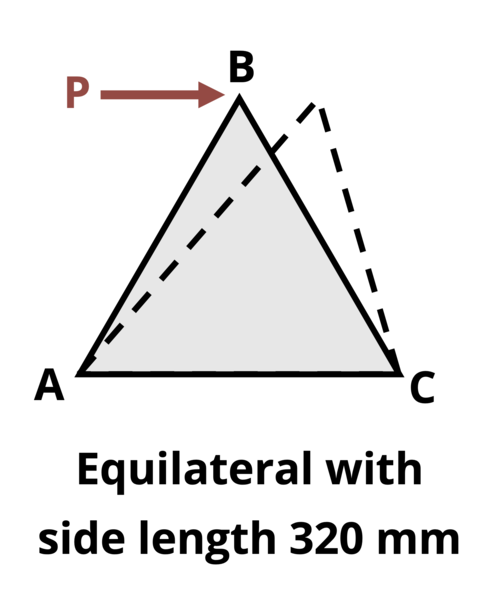
\includegraphics[keepaspectratio]{images/655.png}}
{[}Problem adapted from © Chris Galitz CC BY NC-SA 4.0{]}

\begin{Shaded}
\begin{Highlighting}[]
\NormalTok{\#| standalone: true}
\NormalTok{\#| viewerHeight: 600}
\NormalTok{\#| components: [viewer]}

\NormalTok{from shiny import App, render, ui, reactive}
\NormalTok{import random}
\NormalTok{import asyncio}
\NormalTok{import io}
\NormalTok{import math}
\NormalTok{import string}
\NormalTok{from datetime import datetime}
\NormalTok{from pathlib import Path}

\NormalTok{def generate\_random\_letters(length):}
\NormalTok{    \# Generate a random string of letters of specified length}
\NormalTok{    return \textquotesingle{}\textquotesingle{}.join(random.choice(string.ascii\_lowercase) for \_ in range(length))  }

\NormalTok{problem\_ID="655"}
\NormalTok{L=reactive.Value("\_\_")}
\NormalTok{strain=reactive.Value("\_\_")}
  
\NormalTok{attempts=["Timestamp,Attempt,Answer,Feedback\textbackslash{}n"]}

\NormalTok{app\_ui = ui.page\_fluid(}
\NormalTok{    \#ui.markdown("**Please enter your ID number from your instructor and click to generate your problem**"),}
\NormalTok{    \#ui.input\_text("ID","", placeholder="Enter ID Number Here"),}
\NormalTok{    \#ui.input\_action\_button("generate\_problem", "Generate Problem", class\_="btn{-}primary"),}
\NormalTok{    ui.markdown("**Problem Statement**"),}
\NormalTok{    ui.output\_ui("ui\_problem\_statement"),}
\NormalTok{    ui.input\_text("answer","Your Answer in units of mm", placeholder="Please enter your answer"),}
\NormalTok{    ui.input\_action\_button("submit", "Check Answer", class\_="btn{-}primary"),}
\NormalTok{    \#ui.download\_button("download", "Download File to Submit", class\_="btn{-}success"),}
\NormalTok{)}

\NormalTok{def server(input, output, session):}
\NormalTok{    \# Initialize a counter for attempts}
\NormalTok{    attempt\_counter = reactive.Value(0)}

\NormalTok{    @output}
\NormalTok{    @render.ui}
\NormalTok{    def ui\_problem\_statement():}
\NormalTok{        randomize\_vars()}
\NormalTok{        return[ui.markdown(f"A triangular plate of side length L = \{L()\} mm is subjected to a shear strain of \{strain()\} radians. Determine the distance that corner B displaces."}
\NormalTok{            )}
\NormalTok{        ]}

\NormalTok{    \#@reactive.Effect}
\NormalTok{    \#@reactive.event(input.generate\_problem)}
\NormalTok{    def randomize\_vars():}
\NormalTok{        random.seed(101)}
\NormalTok{        L.set(random.randrange(100,800,10))}
\NormalTok{        strain.set(random.randrange(2,20,1)/100)}

\NormalTok{    @reactive.Effect}
\NormalTok{    @reactive.event(input.submit)}
\NormalTok{    def \_():}
\NormalTok{        attempt\_counter.set(}
\NormalTok{            attempt\_counter() + 1}
\NormalTok{        )  \# Increment the attempt counter on each submission.}

\NormalTok{        \# Calculate the instructor\textquotesingle{}s answer and determine if the user\textquotesingle{}s answer is correct.}
\NormalTok{        ang = math.pi/3{-}2/3*strain()}
\NormalTok{        NewHor = 2*L()*math.sin(math.pi/3)/math.tan(ang)}
\NormalTok{        instr = NewHor{-}L()}
\NormalTok{        if math.isclose(float(input.answer()), instr, rel\_tol=0.01):}
\NormalTok{            check = "*Correct*"}
\NormalTok{            correct\_indicator = "JL"}
\NormalTok{        else:}
\NormalTok{            check = "*Not Correct.*"}
\NormalTok{            correct\_indicator = "JG"}

\NormalTok{        \# Generate random parts for the encoded attempt.}
\NormalTok{        random\_start = generate\_random\_letters(4)}
\NormalTok{        random\_middle = generate\_random\_letters(4)}
\NormalTok{        random\_end = generate\_random\_letters(4)}
\NormalTok{        \#encoded\_attempt = f"\{random\_start\}\{problem\_ID\}{-}\{random\_middle\}\{attempt\_counter()\}\{correct\_indicator\}{-}\{random\_end\}\{input.ID()\}"}

\NormalTok{        \# Store the most recent encoded attempt in a reactive value so it persists across submissions}
\NormalTok{        \#session.encoded\_attempt = reactive.Value(encoded\_attempt)}

\NormalTok{        \# Append the attempt data to the attempts list without the encoded attempt}
\NormalTok{        attempts.append(f"\{datetime.now()\}, \{attempt\_counter()\}, \{input.answer()\}, \{check\}\textbackslash{}n")}

\NormalTok{        \# Show feedback to the user.}
\NormalTok{        feedback = ui.markdown(f"Your answer of \{input.answer()\} is \{check\}.")}
\NormalTok{        m = ui.modal(}
\NormalTok{            feedback,}
\NormalTok{            title="Feedback",}
\NormalTok{            easy\_close=True}
\NormalTok{        )}
\NormalTok{        ui.modal\_show(m)}

\NormalTok{    \#@render.download(filename=lambda: f"Problem\_Log{-}\{problem\_ID\}{-}\{input.ID()\}.csv")}
\NormalTok{    async def download():}
\NormalTok{        \# Start the CSV with the encoded attempt (without label)}
\NormalTok{        final\_encoded = session.encoded\_attempt() if session.encoded\_attempt is not None else "No attempts"}
\NormalTok{        yield f"\{final\_encoded\}\textbackslash{}n\textbackslash{}n"}
        
\NormalTok{        \# Write the header for the remaining CSV data once}
\NormalTok{        yield "Timestamp,Attempt,Answer,Feedback\textbackslash{}n"}
        
\NormalTok{        \# Write the attempts data, ensure that the header from the attempts list is not written again}
\NormalTok{        for attempt in attempts[1:]:  \# Skip the first element which is the header}
\NormalTok{            await asyncio.sleep(0.25)  \# This delay may not be necessary; adjust as needed}
\NormalTok{            yield attempt}

\NormalTok{\# App installation}
\NormalTok{app = App(app\_ui, server)}
\end{Highlighting}
\end{Shaded}

\part{Chapter 4 Problems}

\chapter*{Problem 4.2 - Stress/Strain
Diagram}\label{problem-4.2---stressstrain-diagram}
\addcontentsline{toc}{chapter}{Problem 4.2 - Stress/Strain Diagram}

\markboth{Problem 4.2 - Stress/Strain Diagram}{Problem 4.2 -
Stress/Strain Diagram}

\pandocbounded{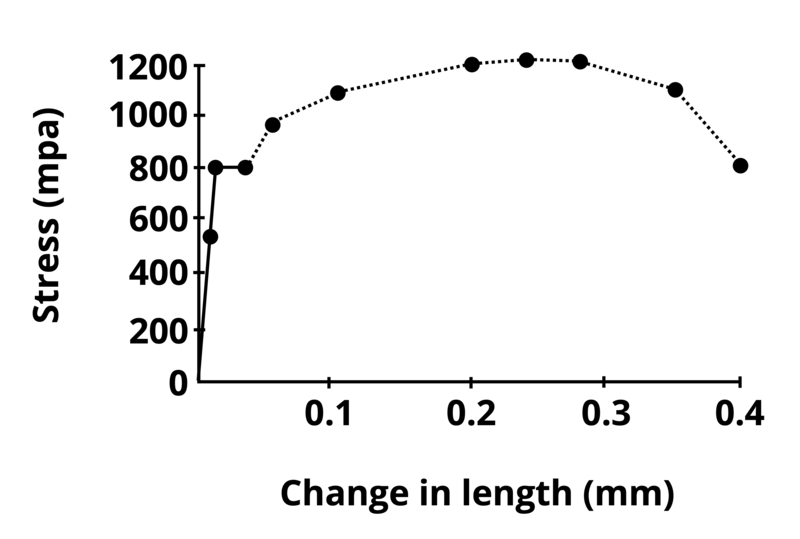
\includegraphics[keepaspectratio]{images/656.png}}
{[}Problem adapted from © Chris Galitz CC BY NC-SA 4.0{]}

\begin{Shaded}
\begin{Highlighting}[]
\NormalTok{\#| standalone: true}
\NormalTok{\#| viewerHeight: 600}
\NormalTok{\#| components: [viewer]}

\NormalTok{from shiny import App, render, ui, reactive}
\NormalTok{import random}
\NormalTok{import asyncio}
\NormalTok{import io}
\NormalTok{import math}
\NormalTok{import string}
\NormalTok{import pandas as pd}
\NormalTok{from datetime import datetime}
\NormalTok{from pathlib import Path}

\NormalTok{def generate\_random\_letters(length):}
\NormalTok{    \# Generate a random string of letters of specified length}
\NormalTok{    return \textquotesingle{}\textquotesingle{}.join(random.choice(string.ascii\_lowercase) for \_ in range(length))  }

\NormalTok{problem\_ID="656"}
\NormalTok{L=reactive.Value("\_\_")}
\NormalTok{P=reactive.Value("\_\_")}
  
\NormalTok{attempts=["Timestamp,Attempt,Answer,Feedback\textbackslash{}n"]}

\NormalTok{app\_ui = ui.page\_fluid(}
\NormalTok{    \#ui.markdown("**Please enter your ID number from your instructor and click to generate your problem**"),}
\NormalTok{    \#ui.input\_text("ID","", placeholder="Enter ID Number Here"),}
\NormalTok{    \#ui.input\_action\_button("generate\_problem", "Generate Problem", class\_="btn{-}primary"),}
\NormalTok{    ui.markdown("**Problem Statement**"),}
\NormalTok{    ui.output\_ui("ui\_problem\_statement"),}
\NormalTok{    ui.input\_text("answer","Your Answer in units of mm", placeholder="Please enter your answer"),}
\NormalTok{    ui.input\_action\_button("submit", "Check Answer", class\_="btn{-}primary"),}
\NormalTok{    \#ui.download\_button("download", "Download File to Submit", class\_="btn{-}success"),}
\NormalTok{)}

\NormalTok{def server(input, output, session):}
\NormalTok{    \# Initialize a counter for attempts}
\NormalTok{    attempt\_counter = reactive.Value(0)}

\NormalTok{    @output}
\NormalTok{    @render.ui}
\NormalTok{    def ui\_problem\_statement():}
\NormalTok{        randomize\_vars()}
\NormalTok{        return[ui.markdown(f"The stress{-}strain diagram for a steel specimen is shown. A rectangular prism tension member of cross{-}sectional area A = 900 mm\textless{}sup\textgreater{}2\textless{}/sup\textgreater{} and initial length L = \{L()\} mm is subjected to load P = \{P()\} kN. Determine the change in length of the member.")]}
    
\NormalTok{    \#@reactive.Effect}
\NormalTok{    \#@reactive.event(input.generate\_problem)}
\NormalTok{    def randomize\_vars():}
\NormalTok{        random.seed(101)}
\NormalTok{        L.set(random.randrange(500,2000,10))}
\NormalTok{        P.set(random.randrange(180,675,1))}

\NormalTok{    @reactive.Effect}
\NormalTok{    @reactive.event(input.submit)}
\NormalTok{    def \_():}
\NormalTok{        attempt\_counter.set(attempt\_counter() + 1)  \# Increment the attempt counter on each submission.}
\NormalTok{        sigma=P()/900*1000}
\NormalTok{        e = sigma/200000}
\NormalTok{        instr = L()*e}
        
\NormalTok{        if math.isclose(float(input.answer()), instr, rel\_tol=0.01):}
\NormalTok{            check = "*Correct*"}
\NormalTok{            correct\_indicator = "JL"}
\NormalTok{        else:}
\NormalTok{            check = "*Not Correct.*"}
\NormalTok{            correct\_indicator = "JG"}

\NormalTok{        \# Generate random parts for the encoded attempt.}
\NormalTok{        random\_start = generate\_random\_letters(4)}
\NormalTok{        random\_middle = generate\_random\_letters(4)}
\NormalTok{        random\_end = generate\_random\_letters(4)}
\NormalTok{        \#encoded\_attempt = f"\{random\_start\}\{problem\_ID\}{-}\{random\_middle\}\{attempt\_counter()\}\{correct\_indicator\}{-}\{random\_end\}\{input.ID()\}"}

\NormalTok{        \# Store the most recent encoded attempt in a reactive value so it persists across submissions}
\NormalTok{        \#session.encoded\_attempt = reactive.Value(encoded\_attempt)}

\NormalTok{        \# Append the attempt data to the attempts list without the encoded attempt}
\NormalTok{        attempts.append(f"\{datetime.now()\}, \{attempt\_counter()\}, \{input.answer()\}, \{check\}\textbackslash{}n")}

\NormalTok{        \# Show feedback to the user.}
\NormalTok{        feedback = ui.markdown(f"Your answer of \{input.answer()\} is \{check\}.")}
\NormalTok{        m = ui.modal(}
\NormalTok{            feedback,}
\NormalTok{            title="Feedback",}
\NormalTok{            easy\_close=True}
\NormalTok{        )}
\NormalTok{        ui.modal\_show(m)}

\NormalTok{    \#@render.download(filename=lambda: f"Problem\_Log{-}\{problem\_ID\}{-}\{input.ID()\}.csv")}
\NormalTok{    async def download():}
\NormalTok{        \# Start the CSV with the encoded attempt (without label)}
\NormalTok{        final\_encoded = session.encoded\_attempt() if session.encoded\_attempt is not None else "No attempts"}
\NormalTok{        yield f"\{final\_encoded\}\textbackslash{}n\textbackslash{}n"}
        
\NormalTok{        \# Write the header for the remaining CSV data once}
\NormalTok{        yield "Timestamp,Attempt,Answer,Feedback\textbackslash{}n"}
        
\NormalTok{        \# Write the attempts data, ensure that the header from the attempts list is not written again}
\NormalTok{        for attempt in attempts[1:]:  \# Skip the first element which is the header}
\NormalTok{            await asyncio.sleep(0.25)  \# This delay may not be necessary; adjust as needed}
\NormalTok{            yield attempt}


\NormalTok{\# App installation}
\NormalTok{app = App(app\_ui, server)}
\end{Highlighting}
\end{Shaded}

\chapter*{Problem 4.5 - Hooke's Law}\label{problem-4.5---hookes-law}
\addcontentsline{toc}{chapter}{Problem 4.5 - Hooke's Law}

\markboth{Problem 4.5 - Hooke's Law}{Problem 4.5 - Hooke's Law}

\begin{figure}[H]

{\centering \pandocbounded{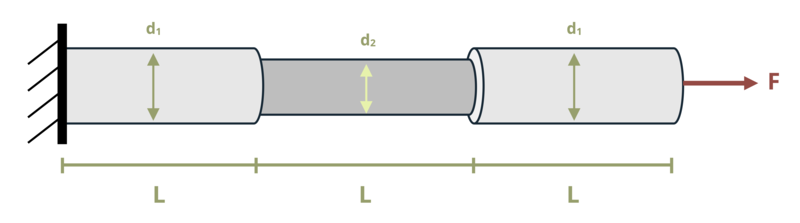
\includegraphics[keepaspectratio]{images/188.png}}

}

\caption{Figure 1: A single force pulls on three cylindrical rods that
are fixed to a wall.}

\end{figure}%

{[}Problem adapted from © Kurt Gramoll CC BY NC-SA 4.0{]}

\begin{Shaded}
\begin{Highlighting}[]
\NormalTok{\#| standalone: true}
\NormalTok{\#| viewerHeight: 600}
\NormalTok{\#| components: [viewer]}

\NormalTok{from shiny import App, render, ui, reactive}
\NormalTok{import random}
\NormalTok{import asyncio}
\NormalTok{import io}
\NormalTok{import math}
\NormalTok{import string}
\NormalTok{from datetime import datetime}
\NormalTok{from pathlib import Path}

\NormalTok{def generate\_random\_letters(length):}
\NormalTok{    \# Generate a random string of letters of specified length}
\NormalTok{    return \textquotesingle{}\textquotesingle{}.join(random.choice(string.ascii\_lowercase) for \_ in range(length))}

\NormalTok{problem\_ID="188"}
\NormalTok{F=reactive.Value("\_\_")}
\NormalTok{L=reactive.Value("\_\_")}
\NormalTok{d1=reactive.Value("\_\_")}
\NormalTok{d2=reactive.Value("\_\_")}
\NormalTok{Esteel = 29000}
\NormalTok{Ealuminum = 10000}


\NormalTok{attempts=["Timestamp,Attempt,Answer,Feedback\textbackslash{}n"]}

\NormalTok{app\_ui = ui.page\_fluid(}
\NormalTok{    \#ui.markdown("**Please enter your ID number from your instructor and click to generate your problem**"),}
\NormalTok{    \#ui.input\_text("ID","", placeholder="Enter ID Number Here"),}
\NormalTok{    \#ui.input\_action\_button("generate\_problem", "Generate Problem", class\_="btn{-}primary"),}
\NormalTok{    ui.markdown("**Problem Statement**"),}
\NormalTok{    ui.output\_ui("ui\_problem\_statement"),}
\NormalTok{    ui.input\_text("answer","Your Answer in units of inches/inches", placeholder="Please enter your answer"),}
\NormalTok{    ui.input\_action\_button("submit", "Check Answer", class\_="btn{-}primary"),}
\NormalTok{    \#ui.download\_button("download", "Download File to Submit", class\_="btn{-}success"),}
\NormalTok{)}


\NormalTok{def server(input, output, session):}
\NormalTok{    \# Initialize a counter for attempts}
\NormalTok{    attempt\_counter = reactive.Value(0)}

\NormalTok{    @output}
\NormalTok{    @render.ui}
\NormalTok{    def ui\_problem\_statement():}
\NormalTok{        randomize\_vars()}
\NormalTok{        return[ui.markdown(f"A single force F = \{F()\} kips pulls on three cylindrical rods, each of length L = \{L()\} in. The aluminum rods have a diameter d\textless{}sub\textgreater{}1\textless{}/sub\textgreater{} = \{d1()\} in., and the steel rods have a diameter d\textless{}sub\textgreater{}2\textless{}/sub\textgreater{} = \{d2()\} in. What is the strain in the steel cylinder? Assume E\textless{}sub\textgreater{}steel\textless{}/sub\textgreater{} = 29,000 ksi and E\textless{}sub\textgreater{}aluminum\textless{}/sub\textgreater{} = 10,000 ksi.")]}
    
\NormalTok{    \#@reactive.Effect}
\NormalTok{    \#@reactive.event(input.generate\_problem)}
\NormalTok{    def randomize\_vars():}
\NormalTok{        random.seed(101)}
\NormalTok{        F.set(random.randrange(20, 300, 1)/10)}
\NormalTok{        L.set(random.randrange(50, 200, 1)/10)}
\NormalTok{        d1.set(random.randrange(10, 50, 1)/10)}
\NormalTok{        d2.set(round(d1()/2, 2))}
        
\NormalTok{    @reactive.Effect}
\NormalTok{    @reactive.event(input.submit)}
\NormalTok{    def \_():}
\NormalTok{        attempt\_counter.set(attempt\_counter() + 1)  \# Increment the attempt counter on each submission.}
\NormalTok{        instr=(F()/(((d2()/2)**2)*math.pi))/Esteel}
\NormalTok{        if math.isclose(float(input.answer()), instr, rel\_tol=0.01):}
\NormalTok{            check = "*Correct*"}
\NormalTok{            correct\_indicator = "JL"}
\NormalTok{        else:}
\NormalTok{            check = "*Not Correct.*"}
\NormalTok{            correct\_indicator = "JG"}

\NormalTok{        \# Generate random parts for the encoded attempt.}
\NormalTok{        random\_start = generate\_random\_letters(4)}
\NormalTok{        random\_middle = generate\_random\_letters(4)}
\NormalTok{        random\_end = generate\_random\_letters(4)}
\NormalTok{        \#encoded\_attempt = f"\{random\_start\}\{problem\_ID\}{-}\{random\_middle\}\{attempt\_counter()\}\{correct\_indicator\}{-}\{random\_end\}\{input.ID()\}"}

\NormalTok{        \# Store the most recent encoded attempt in a reactive value so it persists across submissions}
\NormalTok{        \#session.encoded\_attempt = reactive.Value(encoded\_attempt)}

\NormalTok{        \# Append the attempt data to the attempts list without the encoded attempt}
\NormalTok{        attempts.append(f"\{datetime.now()\}, \{attempt\_counter()\}, \{input.answer()\}, \{check\}\textbackslash{}n")}

\NormalTok{        \# Show feedback to the user.}
\NormalTok{        feedback = ui.markdown(f"Your answer of \{input.answer()\} is \{check\}.")}
\NormalTok{        m = ui.modal(}
\NormalTok{            feedback,}
\NormalTok{            title="Feedback",}
\NormalTok{            easy\_close=True}
\NormalTok{        )}
\NormalTok{        ui.modal\_show(m)}

\NormalTok{    \#@render.download(filename=lambda: f"Problem\_Log{-}\{problem\_ID\}{-}\{input.ID()\}.csv")}
\NormalTok{    async def download():}
\NormalTok{        \# Start the CSV with the encoded attempt (without label)}
\NormalTok{        final\_encoded = session.encoded\_attempt() if session.encoded\_attempt is not None else "No attempts"}
\NormalTok{        yield f"\{final\_encoded\}\textbackslash{}n\textbackslash{}n"}
        
\NormalTok{        \# Write the header for the remaining CSV data once}
\NormalTok{        yield "Timestamp,Attempt,Answer,Feedback\textbackslash{}n"}
        
\NormalTok{        \# Write the attempts data, ensure that the header from the attempts list is not written again}
\NormalTok{        for attempt in attempts[1:]:  \# Skip the first element which is the header}
\NormalTok{            await asyncio.sleep(0.25)  \# This delay may not be necessary; adjust as needed}
\NormalTok{            yield attempt}


\NormalTok{\# App installation}
\NormalTok{app = App(app\_ui, server)}
\end{Highlighting}
\end{Shaded}

\chapter*{Problem 4.6 - Hooke's Law}\label{problem-4.6---hookes-law}
\addcontentsline{toc}{chapter}{Problem 4.6 - Hooke's Law}

\markboth{Problem 4.6 - Hooke's Law}{Problem 4.6 - Hooke's Law}

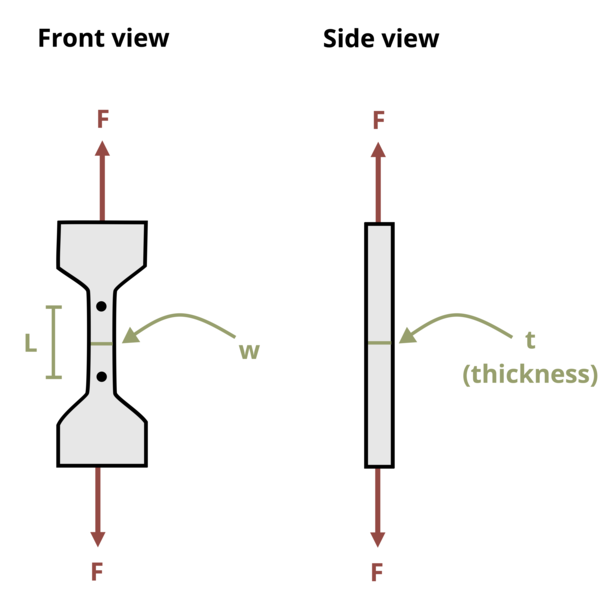
\includegraphics[width=3.125in,height=\textheight,keepaspectratio]{images/194.png}
{[}Problem adapted from © Kurt Gramoll CC BY NC-SA 4.0{]}

\begin{Shaded}
\begin{Highlighting}[]
\NormalTok{\#| standalone: true}
\NormalTok{\#| viewerHeight: 600}
\NormalTok{\#| components: [viewer]}

\NormalTok{from shiny import App, render, ui, reactive}
\NormalTok{import random}
\NormalTok{import asyncio}
\NormalTok{import io}
\NormalTok{import math}
\NormalTok{import string}
\NormalTok{from datetime import datetime}
\NormalTok{from pathlib import Path}

\NormalTok{def generate\_random\_letters(length):}
\NormalTok{    \# Generate a random string of letters of specified length}
\NormalTok{    return \textquotesingle{}\textquotesingle{}.join(random.choice(string.ascii\_lowercase) for \_ in range(length)) }

\NormalTok{problem\_ID="194"}
\NormalTok{F=reactive.Value("\_\_")}
\NormalTok{L=reactive.Value("\_\_")}
\NormalTok{w=reactive.Value("\_\_")}
\NormalTok{t=reactive.Value("\_\_")}
\NormalTok{dL=reactive.Value("\_\_")}


\NormalTok{attempts=["Timestamp,Attempt,Answer,Feedback\textbackslash{}n"]}

\NormalTok{app\_ui = ui.page\_fluid(}
\NormalTok{    \#ui.markdown("**Please enter your ID number from your instructor and click to generate your problem**"),}
\NormalTok{    \#ui.input\_text("ID","", placeholder="Enter ID Number Here"),}
\NormalTok{    \#ui.input\_action\_button("generate\_problem", "Generate Problem", class\_="btn{-}primary"),}
\NormalTok{    ui.markdown("**Problem Statement**"),}
\NormalTok{    ui.output\_ui("ui\_problem\_statement"),}
\NormalTok{    ui.input\_text("answer","Your Answer in units of ksi", placeholder="Please enter your answer"),}
\NormalTok{    ui.input\_action\_button("submit", "Check Answer", class\_="btn{-}primary"),}
\NormalTok{    \#ui.download\_button("download", "Download File to Submit", class\_="btn{-}success"),}
\NormalTok{)}


\NormalTok{def server(input, output, session):}
\NormalTok{    \# Initialize a counter for attempts}
\NormalTok{    attempt\_counter = reactive.Value(0)}

\NormalTok{    @output}
\NormalTok{    @render.ui}
\NormalTok{    def ui\_problem\_statement():}
\NormalTok{        randomize\_vars()}
\NormalTok{        return[ui.markdown(f"A polymer test specimen is subjected to an axial load of F = \{F()\} kips. The central portion of the specimen has an initial length L = \{L()\} in., w = \{w()\} in., and t = \{t()\} in. If the length increases by dL = \{dL()\} in., determine the elastic modulus of the material. ")]}
    
\NormalTok{    \#@reactive.Effect}
\NormalTok{    \#@reactive.event(input.generate\_problem)}
\NormalTok{    def randomize\_vars():}
\NormalTok{        random.seed(101)}
\NormalTok{        F.set(random.randrange(100, 500, 1)/10)}
\NormalTok{        L.set(random.randrange(50, 150, 1)/10)}
\NormalTok{        w.set(round(L()*0.375, 2))}
\NormalTok{        t.set(random.randrange(10, 50, 1)/100)}
\NormalTok{        dL.set(random.randrange(3, 9, 1)/100)}
        
\NormalTok{    @reactive.Effect}
\NormalTok{    @reactive.event(input.submit)}
\NormalTok{    def \_():}
\NormalTok{        attempt\_counter.set(attempt\_counter() + 1)  \# Increment the attempt counter on each submission.}
\NormalTok{        instr= (F()*L())/(dL()*(w()*t()))}
\NormalTok{        if math.isclose(float(input.answer()), instr, rel\_tol=0.01):}
\NormalTok{            check = "*Correct*"}
\NormalTok{            correct\_indicator = "JL"}
\NormalTok{        else:}
\NormalTok{            check = "*Not Correct.*"}
\NormalTok{            correct\_indicator = "JG"}

\NormalTok{        \# Generate random parts for the encoded attempt.}
\NormalTok{        random\_start = generate\_random\_letters(4)}
\NormalTok{        random\_middle = generate\_random\_letters(4)}
\NormalTok{        random\_end = generate\_random\_letters(4)}
\NormalTok{        \#encoded\_attempt = f"\{random\_start\}\{problem\_ID\}{-}\{random\_middle\}\{attempt\_counter()\}\{correct\_indicator\}{-}\{random\_end\}\{input.ID()\}"}

\NormalTok{        \# Store the most recent encoded attempt in a reactive value so it persists across submissions}
\NormalTok{        \#session.encoded\_attempt = reactive.Value(encoded\_attempt)}

\NormalTok{        \# Append the attempt data to the attempts list without the encoded attempt}
\NormalTok{        attempts.append(f"\{datetime.now()\}, \{attempt\_counter()\}, \{input.answer()\}, \{check\}\textbackslash{}n")}

\NormalTok{        \# Show feedback to the user.}
\NormalTok{        feedback = ui.markdown(f"Your answer of \{input.answer()\} is \{check\}.")}
\NormalTok{        m = ui.modal(}
\NormalTok{            feedback,}
\NormalTok{            title="Feedback",}
\NormalTok{            easy\_close=True}
\NormalTok{        )}
\NormalTok{        ui.modal\_show(m)}

\NormalTok{    \#@render.download(filename=lambda: f"Problem\_Log{-}\{problem\_ID\}{-}\{input.ID()\}.csv")}
\NormalTok{    async def download():}
\NormalTok{        \# Start the CSV with the encoded attempt (without label)}
\NormalTok{        final\_encoded = session.encoded\_attempt() if session.encoded\_attempt is not None else "No attempts"}
\NormalTok{        yield f"\{final\_encoded\}\textbackslash{}n\textbackslash{}n"}
        
\NormalTok{        \# Write the header for the remaining CSV data once}
\NormalTok{        yield "Timestamp,Attempt,Answer,Feedback\textbackslash{}n"}
        
\NormalTok{        \# Write the attempts data, ensure that the header from the attempts list is not written again}
\NormalTok{        for attempt in attempts[1:]:  \# Skip the first element which is the header}
\NormalTok{            await asyncio.sleep(0.25)  \# This delay may not be necessary; adjust as needed}
\NormalTok{            yield attempt}


\NormalTok{\# App installation}
\NormalTok{app = App(app\_ui, server)}
\end{Highlighting}
\end{Shaded}

\chapter*{Problem 4.7 - Hooke's Law}\label{problem-4.7---hookes-law}
\addcontentsline{toc}{chapter}{Problem 4.7 - Hooke's Law}

\markboth{Problem 4.7 - Hooke's Law}{Problem 4.7 - Hooke's Law}

{[}Problem adapted from © Chris Galitz CC BY NC-SA 4.0{]}

\begin{Shaded}
\begin{Highlighting}[]
\NormalTok{\#| standalone: true}
\NormalTok{\#| viewerHeight: 600}
\NormalTok{\#| components: [viewer]}

\NormalTok{from shiny import App, render, ui, reactive}
\NormalTok{import random}
\NormalTok{import asyncio}
\NormalTok{import io}
\NormalTok{import math}
\NormalTok{import string}
\NormalTok{from datetime import datetime}
\NormalTok{from pathlib import Path}

\NormalTok{def generate\_random\_letters(length):}
\NormalTok{    \# Generate a random string of letters of specified length}
\NormalTok{    return \textquotesingle{}\textquotesingle{}.join(random.choice(string.ascii\_lowercase) for \_ in range(length))  }

\NormalTok{problem\_ID="657"}
\NormalTok{d=reactive.Value("\_\_")}
\NormalTok{L=reactive.Value("\_\_")}
\NormalTok{P=reactive.Value("\_\_")}
\NormalTok{elong=reactive.Value("\_\_")}
  
\NormalTok{attempts=["Timestamp,Attempt,Answer,Feedback\textbackslash{}n"]}

\NormalTok{app\_ui = ui.page\_fluid(}
\NormalTok{    \#ui.markdown("**Please enter your ID number from your instructor and click to generate your problem**"),}
\NormalTok{    \#ui.input\_text("ID","", placeholder="Enter ID Number Here"),}
\NormalTok{    \#ui.input\_action\_button("generate\_problem", "Generate Problem", class\_="btn{-}primary"),}
\NormalTok{    ui.markdown("**Problem Statement**"),}
\NormalTok{    ui.output\_ui("ui\_problem\_statement"),}
\NormalTok{    ui.input\_text("answer","Your Answer in units of ksi", placeholder="Please enter your answer"),}
\NormalTok{    ui.input\_action\_button("submit", "Check Answer", class\_="btn{-}primary"),}
\NormalTok{    \#ui.download\_button("download", "Download File to Submit", class\_="btn{-}success"),}
\NormalTok{)}

\NormalTok{def server(input, output, session):}
\NormalTok{    \# Initialize a counter for attempts}
\NormalTok{    attempt\_counter = reactive.Value(0)}

\NormalTok{    @output}
\NormalTok{    @render.ui}
\NormalTok{    def ui\_problem\_statement():}
\NormalTok{        randomize\_vars()}
\NormalTok{        return[ui.markdown(f"A round bar of diameter d = \{d()\} in. and length L = \{L()\} in. is subjected to axial load P = \{P()\} lb. If the elongation of the bar is \{elong()\} in., and assuming elastic behavior, determine the elastic modulus of the bar.")]}
    
\NormalTok{    \#@reactive.Effect}
\NormalTok{    \#@reactive.event(input.generate\_problem)}
\NormalTok{    def randomize\_vars():}
\NormalTok{        random.seed(101)}
\NormalTok{        d.set(random.randrange(3,15,1)/10)}
\NormalTok{        L.set(random.randrange(100,200,1)/10)}
\NormalTok{        P.set(random.randrange(750,1500,10))}
\NormalTok{        elong.set(random.randrange(50,200,1)/1000)}
        
\NormalTok{    @reactive.Effect}
\NormalTok{    @reactive.event(input.submit)}
\NormalTok{    def \_():}
\NormalTok{        attempt\_counter.set(attempt\_counter() + 1)  \# Increment the attempt counter on each submission.}
\NormalTok{        A = math.pi*(d()**2)/4}
\NormalTok{        sigma = P()/A}
\NormalTok{        epsilon = elong()/L()}
\NormalTok{        instr= sigma/epsilon/1000}
\NormalTok{        if math.isclose(float(input.answer()), instr, rel\_tol=0.01):}
\NormalTok{            check = "*Correct*"}
\NormalTok{            correct\_indicator = "JL"}
\NormalTok{        else:}
\NormalTok{            check = "*Not Correct.*"}
\NormalTok{            correct\_indicator = "JG"}

\NormalTok{        \# Generate random parts for the encoded attempt.}
\NormalTok{        random\_start = generate\_random\_letters(4)}
\NormalTok{        random\_middle = generate\_random\_letters(4)}
\NormalTok{        random\_end = generate\_random\_letters(4)}
\NormalTok{        \#encoded\_attempt = f"\{random\_start\}\{problem\_ID\}{-}\{random\_middle\}\{attempt\_counter()\}\{correct\_indicator\}{-}\{random\_end\}\{input.ID()\}"}

\NormalTok{        \# Store the most recent encoded attempt in a reactive value so it persists across submissions}
\NormalTok{        \#session.encoded\_attempt = reactive.Value(encoded\_attempt)}

\NormalTok{        \# Append the attempt data to the attempts list without the encoded attempt}
\NormalTok{        attempts.append(f"\{datetime.now()\}, \{attempt\_counter()\}, \{input.answer()\}, \{check\}\textbackslash{}n")}

\NormalTok{        \# Show feedback to the user.}
\NormalTok{        feedback = ui.markdown(f"Your answer of \{input.answer()\} is \{check\}.")}
\NormalTok{        m = ui.modal(}
\NormalTok{            feedback,}
\NormalTok{            title="Feedback",}
\NormalTok{            easy\_close=True}
\NormalTok{        )}
\NormalTok{        ui.modal\_show(m)}

\NormalTok{    \#@render.download(filename=lambda: f"Problem\_Log{-}\{problem\_ID\}{-}\{input.ID()\}.csv")}
\NormalTok{    async def download():}
\NormalTok{        \# Start the CSV with the encoded attempt (without label)}
\NormalTok{        final\_encoded = session.encoded\_attempt() if session.encoded\_attempt is not None else "No attempts"}
\NormalTok{        yield f"\{final\_encoded\}\textbackslash{}n\textbackslash{}n"}
        
\NormalTok{        \# Write the header for the remaining CSV data once}
\NormalTok{        yield "Timestamp,Attempt,Answer,Feedback\textbackslash{}n"}
        
\NormalTok{        \# Write the attempts data, ensure that the header from the attempts list is not written again}
\NormalTok{        for attempt in attempts[1:]:  \# Skip the first element which is the header}
\NormalTok{            await asyncio.sleep(0.25)  \# This delay may not be necessary; adjust as needed}
\NormalTok{            yield attempt}

\NormalTok{\# App installation}
\NormalTok{app = App(app\_ui, server)}
\end{Highlighting}
\end{Shaded}

\chapter*{Problem 4.10 - Poisson's
Ratio}\label{problem-4.10---poissons-ratio}
\addcontentsline{toc}{chapter}{Problem 4.10 - Poisson's Ratio}

\markboth{Problem 4.10 - Poisson's Ratio}{Problem 4.10 - Poisson's
Ratio}

\begin{figure}[H]

{\centering \pandocbounded{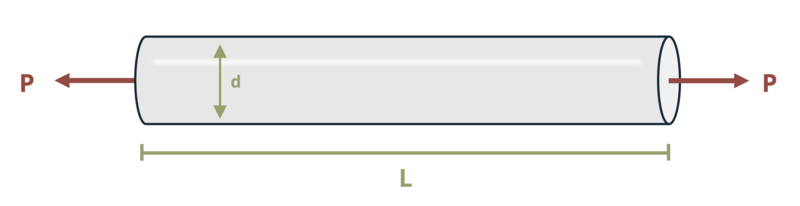
\includegraphics[keepaspectratio]{images/206.png}}

}

\caption{Figure 1: A circular road is placed in tension with an axial
load.}

\end{figure}%

{[}Problem adapted from © Kurt Gramoll CC BY NC-SA 4.0{]}

\begin{Shaded}
\begin{Highlighting}[]
\NormalTok{\#| standalone: true}
\NormalTok{\#| viewerHeight: 600}
\NormalTok{\#| components: [viewer]}

\NormalTok{from shiny import App, render, ui, reactive}
\NormalTok{import random}
\NormalTok{import asyncio}
\NormalTok{import io}
\NormalTok{import math}
\NormalTok{import string}
\NormalTok{from datetime import datetime}
\NormalTok{from pathlib import Path}

\NormalTok{def generate\_random\_letters(length):}
\NormalTok{    \# Generate a random string of letters of specified length}
\NormalTok{    return \textquotesingle{}\textquotesingle{}.join(random.choice(string.ascii\_lowercase) for \_ in range(length)) }

\NormalTok{problem\_ID="206"}
\NormalTok{P=reactive.Value("\_\_")}
\NormalTok{E=reactive.Value("\_\_")}
\NormalTok{L=reactive.Value("\_\_")}
\NormalTok{d=reactive.Value("\_\_")}

\NormalTok{attempts=["Timestamp,Attempt,Answer,Feedback\textbackslash{}n"]}

\NormalTok{app\_ui = ui.page\_fluid(}
\NormalTok{    \#ui.markdown("**Please enter your ID number from your instructor and click to generate your problem**"),}
\NormalTok{    \#ui.input\_text("ID","", placeholder="Enter ID Number Here"),}
\NormalTok{    \#ui.input\_action\_button("generate\_problem", "Generate Problem", class\_="btn{-}primary"),}
\NormalTok{    ui.markdown("**Problem Statement**"),}
\NormalTok{    ui.output\_ui("ui\_problem\_statement"),}
\NormalTok{    ui.input\_text("answer","Your Answer", placeholder="Please enter your answer"),}
\NormalTok{    ui.input\_action\_button("submit", "Check Answer", class\_="btn{-}primary"),}
\NormalTok{    \#ui.download\_button("download", "Download File to Submit", class\_="btn{-}success"),}
\NormalTok{)}

\NormalTok{def server(input, output, session):}
\NormalTok{    \# Initialize a counter for attempts}
\NormalTok{    attempt\_counter = reactive.Value(0)}

\NormalTok{    @output}
\NormalTok{    @render.ui}
\NormalTok{    def ui\_problem\_statement():}
\NormalTok{        randomize\_vars()}
\NormalTok{        return[ui.markdown(f"A circular rod of an unknown metallic alloy is placed in tension with a P = \{P()\} kip axial load. The length of the rod is L = \{L()\} in. and the diameter is d = \{d()\} in. After applying the load, the rod length increases by 0.0035 in and the diameter decreases by 0.00014 in. What is the Poisson\textquotesingle{}s ratio of the alloy?")]}
    
\NormalTok{    \#@reactive.Effect}
\NormalTok{    \#@reactive.event(input.generate\_problem)}
\NormalTok{    def randomize\_vars():}
\NormalTok{        random.seed(101)}
\NormalTok{        P.set(random.randrange(20, 200, 1)/10)}
\NormalTok{        L.set(random.randrange(10, 20, 1))}
\NormalTok{        E.set(random.randrange(20, 40, 1)/100)}
\NormalTok{        d.set(round((.00014*L())/(.0035*E()), 1))}
        
\NormalTok{    @reactive.Effect}
\NormalTok{    @reactive.event(input.submit)}
\NormalTok{    def \_():}
\NormalTok{        attempt\_counter.set(attempt\_counter() + 1)  \# Increment the attempt counter on each submission.}
       
\NormalTok{        instr= {-}({-}.00014/d())/(.0035/L())}
\NormalTok{        if math.isclose(float(input.answer()), instr, rel\_tol=0.01):}
\NormalTok{            check = "*Correct*"}
\NormalTok{            correct\_indicator = "JL"}
\NormalTok{        else:}
\NormalTok{            check = "*Not Correct.*"}
\NormalTok{            correct\_indicator = "JG"}

\NormalTok{        \# Generate random parts for the encoded attempt.}
\NormalTok{        random\_start = generate\_random\_letters(4)}
\NormalTok{        random\_middle = generate\_random\_letters(4)}
\NormalTok{        random\_end = generate\_random\_letters(4)}
\NormalTok{        \#encoded\_attempt = f"\{random\_start\}\{problem\_ID\}{-}\{random\_middle\}\{attempt\_counter()\}\{correct\_indicator\}{-}\{random\_end\}\{input.ID()\}"}

\NormalTok{        \# Store the most recent encoded attempt in a reactive value so it persists across submissions}
\NormalTok{        \#session.encoded\_attempt = reactive.Value(encoded\_attempt)}

\NormalTok{        \# Append the attempt data to the attempts list without the encoded attempt}
\NormalTok{        attempts.append(f"\{datetime.now()\}, \{attempt\_counter()\}, \{input.answer()\}, \{check\}\textbackslash{}n")}

\NormalTok{        \# Show feedback to the user.}
\NormalTok{        feedback = ui.markdown(f"Your answer of \{input.answer()\} is \{check\}.")}
\NormalTok{        m = ui.modal(}
\NormalTok{            feedback,}
\NormalTok{            title="Feedback",}
\NormalTok{            easy\_close=True}
\NormalTok{        )}
\NormalTok{        ui.modal\_show(m)}

\NormalTok{    \#@render.download(filename=lambda: f"Problem\_Log{-}\{problem\_ID\}{-}\{input.ID()\}.csv")}
\NormalTok{    async def download():}
\NormalTok{        \# Start the CSV with the encoded attempt (without label)}
\NormalTok{        final\_encoded = session.encoded\_attempt() if session.encoded\_attempt is not None else "No attempts"}
\NormalTok{        yield f"\{final\_encoded\}\textbackslash{}n\textbackslash{}n"}
        
\NormalTok{        \# Write the header for the remaining CSV data once}
\NormalTok{        yield "Timestamp,Attempt,Answer,Feedback\textbackslash{}n"}
        
\NormalTok{        \# Write the attempts data, ensure that the header from the attempts list is not written again}
\NormalTok{        for attempt in attempts[1:]:  \# Skip the first element which is the header}
\NormalTok{            await asyncio.sleep(0.25)  \# This delay may not be necessary; adjust as needed}
\NormalTok{            yield attempt}

\NormalTok{\# App installation}
\NormalTok{app = App(app\_ui, server)}
\end{Highlighting}
\end{Shaded}

\chapter*{Problem 4.11 - Poisson's
Ratio}\label{problem-4.11---poissons-ratio}
\addcontentsline{toc}{chapter}{Problem 4.11 - Poisson's Ratio}

\markboth{Problem 4.11 - Poisson's Ratio}{Problem 4.11 - Poisson's
Ratio}

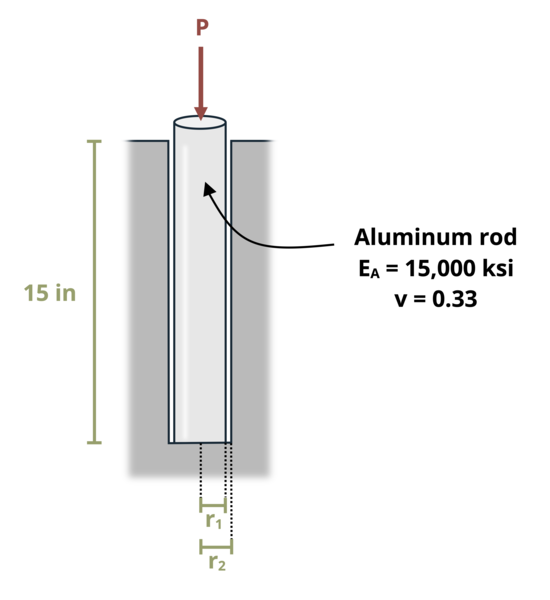
\includegraphics[width=4.16667in,height=\textheight,keepaspectratio]{images/213.png}
{[}Problem adapted from © Kurt Gramoll CC BY NC-SA 4.0{]}

\begin{Shaded}
\begin{Highlighting}[]
\NormalTok{\#| standalone: true}
\NormalTok{\#| viewerHeight: 600}
\NormalTok{\#| components: [viewer]}

\NormalTok{from shiny import App, render, ui, reactive}
\NormalTok{import random}
\NormalTok{import asyncio}
\NormalTok{import io}
\NormalTok{import math}
\NormalTok{import string}
\NormalTok{from datetime import datetime}
\NormalTok{from pathlib import Path}

\NormalTok{def generate\_random\_letters(length):}
\NormalTok{    \# Generate a random string of letters of specified length}
\NormalTok{    return \textquotesingle{}\textquotesingle{}.join(random.choice(string.ascii\_lowercase) for \_ in range(length)) }

\NormalTok{problem\_ID="213"}
\NormalTok{r1=reactive.Value("\_\_")}
\NormalTok{r2=reactive.Value("\_\_")}
\NormalTok{E=15000}
\NormalTok{v=0.33}


\NormalTok{attempts=["Timestamp,Attempt,Answer,Feedback\textbackslash{}n"]}

\NormalTok{app\_ui = ui.page\_fluid(}
\NormalTok{    \#ui.markdown("**Please enter your ID number from your instructor and click to generate your problem**"),}
\NormalTok{    \#ui.input\_text("ID","", placeholder="Enter ID Number Here"),}
\NormalTok{    \#ui.input\_action\_button("generate\_problem", "Generate Problem", class\_="btn{-}primary"),}
\NormalTok{    ui.markdown("**Problem Statement**"),}
\NormalTok{    ui.output\_ui("ui\_problem\_statement"),}
\NormalTok{    ui.input\_text("answer","Your Answer in units of kip", placeholder="Please enter your answer"),}
\NormalTok{    ui.input\_action\_button("submit", "Check Answer", class\_="btn{-}primary"),}
\NormalTok{    \#ui.download\_button("download", "Download File to Submit", class\_="btn{-}success"),}
\NormalTok{)}


\NormalTok{def server(input, output, session):}
\NormalTok{    \# Initialize a counter for attempts}
\NormalTok{    attempt\_counter = reactive.Value(0)}

\NormalTok{    @output}
\NormalTok{    @render.ui}
\NormalTok{    def ui\_problem\_statement():}
\NormalTok{        randomize\_vars()}
\NormalTok{        return[ui.markdown(f"An aluminum circular rod of radius r\textless{}sub\textgreater{}1\textless{}/sub\textgreater{} = \{r1()\} in is inserted into space that is slightly wider than the rod, where r\textless{}sub\textgreater{}2\textless{}/sub\textgreater{} = \{r2()\} in. What load P is needed so that the rod expands and fills the space in the radial direction? Assume E = 15,000 ksi and v = 0.33. ")]}
    
\NormalTok{    \#@reactive.Effect}
\NormalTok{    \#@reactive.event(input.generate\_problem)}
\NormalTok{    def randomize\_vars():}
\NormalTok{        random.seed(101)}
\NormalTok{        r1.set(random.randrange(10, 50, 1)/10)}
\NormalTok{        r2.set((r1() + random.randrange(1, 10, 1)/1000))}
        
\NormalTok{    @reactive.Effect}
\NormalTok{    @reactive.event(input.submit)}
\NormalTok{    def \_():}
\NormalTok{        attempt\_counter.set(attempt\_counter() + 1)  \# Increment the attempt counter on each submission.}
\NormalTok{        Ex = (r1() {-} r2())/r1()}
\NormalTok{        sigmay = (Ex*E)/({-}v)}
\NormalTok{        instr= sigmay*math.pi*r1()**2}
\NormalTok{        if math.isclose(float(input.answer()), instr, rel\_tol=0.01):}
\NormalTok{            check = "*Correct*"}
\NormalTok{            correct\_indicator = "JL"}
\NormalTok{        else:}
\NormalTok{            check = "*Not Correct.*"}
\NormalTok{            correct\_indicator = "JG"}

\NormalTok{        \# Generate random parts for the encoded attempt.}
\NormalTok{        random\_start = generate\_random\_letters(4)}
\NormalTok{        random\_middle = generate\_random\_letters(4)}
\NormalTok{        random\_end = generate\_random\_letters(4)}
\NormalTok{        \#encoded\_attempt = f"\{random\_start\}\{problem\_ID\}{-}\{random\_middle\}\{attempt\_counter()\}\{correct\_indicator\}{-}\{random\_end\}\{input.ID()\}"}

\NormalTok{        \# Store the most recent encoded attempt in a reactive value so it persists across submissions}
\NormalTok{        \#session.encoded\_attempt = reactive.Value(encoded\_attempt)}

\NormalTok{        \# Append the attempt data to the attempts list without the encoded attempt}
\NormalTok{        attempts.append(f"\{datetime.now()\}, \{attempt\_counter()\}, \{input.answer()\}, \{check\}\textbackslash{}n")}

\NormalTok{        \# Show feedback to the user.}
\NormalTok{        feedback = ui.markdown(f"Your answer of \{input.answer()\} is \{check\}.")}
\NormalTok{        m = ui.modal(}
\NormalTok{            feedback,}
\NormalTok{            title="Feedback",}
\NormalTok{            easy\_close=True}
\NormalTok{        )}
\NormalTok{        ui.modal\_show(m)}

\NormalTok{    \#@render.download(filename=lambda: f"Problem\_Log{-}\{problem\_ID\}{-}\{input.ID()\}.csv")}
\NormalTok{    async def download():}
\NormalTok{        \# Start the CSV with the encoded attempt (without label)}
\NormalTok{        final\_encoded = session.encoded\_attempt() if session.encoded\_attempt is not None else "No attempts"}
\NormalTok{        yield f"\{final\_encoded\}\textbackslash{}n\textbackslash{}n"}
        
\NormalTok{        \# Write the header for the remaining CSV data once}
\NormalTok{        yield "Timestamp,Attempt,Answer,Feedback\textbackslash{}n"}
        
\NormalTok{        \# Write the attempts data, ensure that the header from the attempts list is not written again}
\NormalTok{        for attempt in attempts[1:]:  \# Skip the first element which is the header}
\NormalTok{            await asyncio.sleep(0.25)  \# This delay may not be necessary; adjust as needed}
\NormalTok{            yield attempt}


\NormalTok{\# App installation}
\NormalTok{app = App(app\_ui, server)}
\end{Highlighting}
\end{Shaded}

\chapter*{Problem 4.12 - Poisson's
Ratio}\label{problem-4.12---poissons-ratio}
\addcontentsline{toc}{chapter}{Problem 4.12 - Poisson's Ratio}

\markboth{Problem 4.12 - Poisson's Ratio}{Problem 4.12 - Poisson's
Ratio}

\pandocbounded{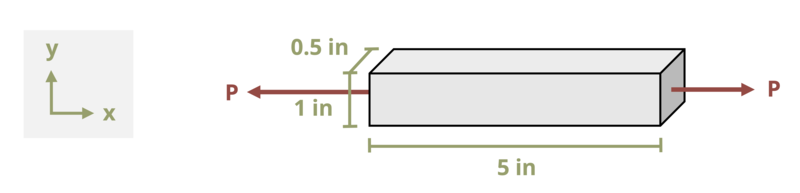
\includegraphics[keepaspectratio]{images/216.png}}
{[}Problem adapted from © Kurt Gramoll CC BY NC-SA 4.0{]}

\begin{Shaded}
\begin{Highlighting}[]
\NormalTok{\#| standalone: true}
\NormalTok{\#| viewerHeight: 600}
\NormalTok{\#| components: [viewer]}

\NormalTok{from shiny import App, render, ui, reactive}
\NormalTok{import random}
\NormalTok{import asyncio}
\NormalTok{import io}
\NormalTok{import math}
\NormalTok{import string}
\NormalTok{from datetime import datetime}
\NormalTok{from pathlib import Path}

\NormalTok{def generate\_random\_letters(length):}
\NormalTok{    \# Generate a random string of letters of specified length}
\NormalTok{    return \textquotesingle{}\textquotesingle{}.join(random.choice(string.ascii\_lowercase) for \_ in range(length)) }

\NormalTok{problem\_ID="216"}
\NormalTok{d1=reactive.Value("\_\_")}
\NormalTok{d2=reactive.Value("\_\_")}


\NormalTok{attempts=["Timestamp,Attempt,Answer,Feedback\textbackslash{}n"]}

\NormalTok{app\_ui = ui.page\_fluid(}
\NormalTok{    \#ui.markdown("**Please enter your ID number from your instructor and click to generate your problem**"),}
\NormalTok{    \#ui.input\_text("ID","", placeholder="Enter ID Number Here"),}
\NormalTok{    \#ui.input\_action\_button("generate\_problem", "Generate Problem", class\_="btn{-}primary"),}
\NormalTok{    ui.markdown("**Problem Statement**"),}
\NormalTok{    ui.output\_ui("ui\_problem\_statement"),}
\NormalTok{    ui.input\_text("answer","Your Answer", placeholder="Please enter your answer"),}
\NormalTok{    ui.input\_action\_button("submit", "Check Answer", class\_="btn{-}primary"),}
\NormalTok{    \#ui.download\_button("download", "Download File to Submit", class\_="btn{-}success"),}
\NormalTok{)}


\NormalTok{def server(input, output, session):}
\NormalTok{    \# Initialize a counter for attempts}
\NormalTok{    attempt\_counter = reactive.Value(0)}

\NormalTok{    @output}
\NormalTok{    @render.ui}
\NormalTok{    def ui\_problem\_statement():}
\NormalTok{        randomize\_vars()}
\NormalTok{        return[ui.markdown(f"A rectangular bar is pulled in tension by a load P in the x{-}direction. The bar deflects by δ\textless{}sub\textgreater{}1\textless{}/sub\textgreater{} = \{d1()\} in and δ\textless{}sub\textgreater{}2\textless{}/sub\textgreater{} = {-} \{d2()\} in, in the x{-} and y{-}direction, respectively. The length in the x{-}direction is 5 in, and the length in the y direction is 1 in. What is the Poisson\textquotesingle{}s ratio of the material? The z{-}direction deflection is not known. ")]}
    
\NormalTok{    \#@reactive.Effect}
\NormalTok{    \#@reactive.event(input.generate\_problem)}
\NormalTok{    def randomize\_vars():}
\NormalTok{        random.seed(101)}
\NormalTok{        d1.set(random.randrange(20, 50, 1)/1000)}
\NormalTok{        d2.set(random.randrange(10, 20, 1)/10000)}
        
\NormalTok{    @reactive.Effect}
\NormalTok{    @reactive.event(input.submit)}
\NormalTok{    def \_():}
\NormalTok{        attempt\_counter.set(attempt\_counter() + 1)  \# Increment the attempt counter on each submission.}
\NormalTok{        instr= {-}({-}d2()/1)/(d1()/5)}
\NormalTok{        if math.isclose(float(input.answer()), instr, rel\_tol=0.01):}
\NormalTok{            check = "*Correct*"}
\NormalTok{            correct\_indicator = "JL"}
\NormalTok{        else:}
\NormalTok{            check = "*Not Correct.*"}
\NormalTok{            correct\_indicator = "JG"}

\NormalTok{        \# Generate random parts for the encoded attempt.}
\NormalTok{        random\_start = generate\_random\_letters(4)}
\NormalTok{        random\_middle = generate\_random\_letters(4)}
\NormalTok{        random\_end = generate\_random\_letters(4)}
\NormalTok{        \#encoded\_attempt = f"\{random\_start\}\{problem\_ID\}{-}\{random\_middle\}\{attempt\_counter()\}\{correct\_indicator\}{-}\{random\_end\}\{input.ID()\}"}

\NormalTok{        \# Store the most recent encoded attempt in a reactive value so it persists across submissions}
\NormalTok{        \#session.encoded\_attempt = reactive.Value(encoded\_attempt)}

\NormalTok{        \# Append the attempt data to the attempts list without the encoded attempt}
\NormalTok{        attempts.append(f"\{datetime.now()\}, \{attempt\_counter()\}, \{input.answer()\}, \{check\}\textbackslash{}n")}

\NormalTok{        \# Show feedback to the user.}
\NormalTok{        feedback = ui.markdown(f"Your answer of \{input.answer()\} is \{check\}.")}
\NormalTok{        m = ui.modal(}
\NormalTok{            feedback,}
\NormalTok{            title="Feedback",}
\NormalTok{            easy\_close=True}
\NormalTok{        )}
\NormalTok{        ui.modal\_show(m)}

\NormalTok{    \#@render.download(filename=lambda: f"Problem\_Log{-}\{problem\_ID\}{-}\{input.ID()\}.csv")}
\NormalTok{    async def download():}
\NormalTok{        \# Start the CSV with the encoded attempt (without label)}
\NormalTok{        final\_encoded = session.encoded\_attempt() if session.encoded\_attempt is not None else "No attempts"}
\NormalTok{        yield f"\{final\_encoded\}\textbackslash{}n\textbackslash{}n"}
        
\NormalTok{        \# Write the header for the remaining CSV data once}
\NormalTok{        yield "Timestamp,Attempt,Answer,Feedback\textbackslash{}n"}
        
\NormalTok{        \# Write the attempts data, ensure that the header from the attempts list is not written again}
\NormalTok{        for attempt in attempts[1:]:  \# Skip the first element which is the header}
\NormalTok{            await asyncio.sleep(0.25)  \# This delay may not be necessary; adjust as needed}
\NormalTok{            yield attempt}


\NormalTok{\# App installation}
\NormalTok{app = App(app\_ui, server)}
\end{Highlighting}
\end{Shaded}

\chapter*{Problem 4.17 - Shear
Stress/Strain}\label{problem-4.17---shear-stressstrain}
\addcontentsline{toc}{chapter}{Problem 4.17 - Shear Stress/Strain}

\markboth{Problem 4.17 - Shear Stress/Strain}{Problem 4.17 - Shear
Stress/Strain}

\pandocbounded{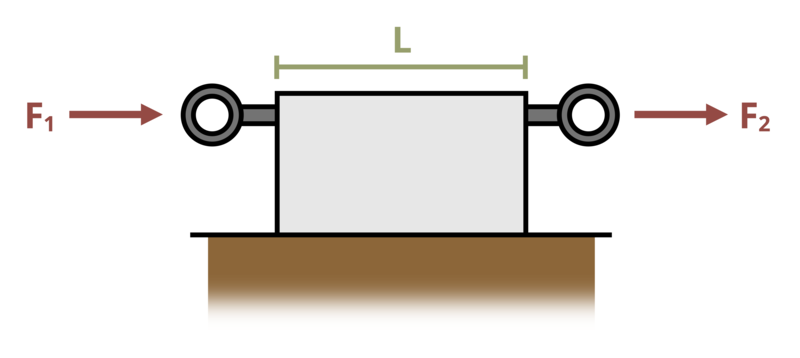
\includegraphics[keepaspectratio]{images/218.png}}
{[}Problem adapted from © Kurt Gramoll CC BY NC-SA 4.0{]}

\begin{Shaded}
\begin{Highlighting}[]
\NormalTok{\#| standalone: true}
\NormalTok{\#| viewerHeight: 600}
\NormalTok{\#| components: [viewer]}

\NormalTok{from shiny import App, render, ui, reactive}
\NormalTok{import random}
\NormalTok{import asyncio}
\NormalTok{import io}
\NormalTok{import math}
\NormalTok{import string}
\NormalTok{from datetime import datetime}
\NormalTok{from pathlib import Path}

\NormalTok{def generate\_random\_letters(length):}
\NormalTok{    \# Generate a random string of letters of specified length}
\NormalTok{    return \textquotesingle{}\textquotesingle{}.join(random.choice(string.ascii\_lowercase) for \_ in range(length))}

\NormalTok{problem\_ID="218"}
\NormalTok{F2=reactive.Value("\_\_")}
\NormalTok{F1=reactive.Value("\_\_")}
\NormalTok{L=reactive.Value("\_\_")}
\NormalTok{d=reactive.Value("\_\_")}
  
\NormalTok{attempts=["Timestamp,Attempt,Answer,Feedback\textbackslash{}n"]}

\NormalTok{app\_ui = ui.page\_fluid(}
\NormalTok{    \#ui.markdown("**Please enter your ID number from your instructor and click to generate your problem**"),}
\NormalTok{    \#ui.input\_text("ID","", placeholder="Enter ID Number Here"),}
\NormalTok{    \#ui.input\_action\_button("generate\_problem", "Generate Problem", class\_="btn{-}primary"),}
\NormalTok{    ui.markdown("**Problem Statement**"),}
\NormalTok{    ui.output\_ui("ui\_problem\_statement"),}
\NormalTok{    ui.input\_text("answer","Your Answer in units of radians", placeholder="Please enter your answer"),}
\NormalTok{    ui.input\_action\_button("submit", "Check Answer", class\_="btn{-}primary"),}
\NormalTok{    \#ui.download\_button("download", "Download File to Submit", class\_="btn{-}success"),}
\NormalTok{)}

\NormalTok{def server(input, output, session):}
\NormalTok{    \# Initialize a counter for attempts}
\NormalTok{    attempt\_counter = reactive.Value(0)}

\NormalTok{    @output}
\NormalTok{    @render.ui}
\NormalTok{    def ui\_problem\_statement():}
\NormalTok{        randomize\_vars()}
\NormalTok{        return[ui.markdown(f"Force F\textless{}sub\textgreater{}1\textless{}/sub\textgreater{} = \{F1()\} lb and F\textless{}sub\textgreater{}2\textless{}/sub\textgreater{} = \{F2()\} lb are applied to a rubber block of length L = \{L()\} in. as shown. The depth of the block is \{d()\} in. Determine the shear strain in the block, assuming ν = 0.49 and E = 500 psi.")]}
    
\NormalTok{    \#@reactive.Effect}
\NormalTok{    \#@reactive.event(input.generate\_problem)}
\NormalTok{    def randomize\_vars():}
\NormalTok{        random.seed(101)}
\NormalTok{        F2.set(random.randrange(10,50,1))}
\NormalTok{        F1.set(F2()+random.randrange(5,20,1))}
\NormalTok{        L.set(random.randrange(30,60,1))}
\NormalTok{        d.set(random.randrange(30,60,1))}
        
\NormalTok{    @reactive.Effect}
\NormalTok{    @reactive.event(input.submit)}
\NormalTok{    def \_():}
\NormalTok{        attempt\_counter.set(attempt\_counter() + 1)  \# Increment the attempt counter on each submission.}
\NormalTok{        tau = (F1()+F2())/(L()*d())}
\NormalTok{        G = 500/(2*(1+0.49))}
\NormalTok{        instr = tau/G}
\NormalTok{        if math.isclose(float(input.answer()), instr, rel\_tol=0.01):}
\NormalTok{            check = "*Correct*"}
\NormalTok{            correct\_indicator = "JL"}
\NormalTok{        else:}
\NormalTok{            check = "*Not Correct.*"}
\NormalTok{            correct\_indicator = "JG"}

\NormalTok{        \# Generate random parts for the encoded attempt.}
\NormalTok{        random\_start = generate\_random\_letters(4)}
\NormalTok{        random\_middle = generate\_random\_letters(4)}
\NormalTok{        random\_end = generate\_random\_letters(4)}
\NormalTok{        \#encoded\_attempt = f"\{random\_start\}\{problem\_ID\}{-}\{random\_middle\}\{attempt\_counter()\}\{correct\_indicator\}{-}\{random\_end\}\{input.ID()\}"}

\NormalTok{        \# Store the most recent encoded attempt in a reactive value so it persists across submissions}
\NormalTok{        \#session.encoded\_attempt = reactive.Value(encoded\_attempt)}

\NormalTok{        \# Append the attempt data to the attempts list without the encoded attempt}
\NormalTok{        attempts.append(f"\{datetime.now()\}, \{attempt\_counter()\}, \{input.answer()\}, \{check\}\textbackslash{}n")}

\NormalTok{        \# Show feedback to the user.}
\NormalTok{        feedback = ui.markdown(f"Your answer of \{input.answer()\} is \{check\}.")}
\NormalTok{        m = ui.modal(}
\NormalTok{            feedback,}
\NormalTok{            title="Feedback",}
\NormalTok{            easy\_close=True}
\NormalTok{        )}
\NormalTok{        ui.modal\_show(m)}

\NormalTok{    \#@render.download(filename=lambda: f"Problem\_Log{-}\{problem\_ID\}{-}\{input.ID()\}.csv")}
\NormalTok{    async def download():}
\NormalTok{        \# Start the CSV with the encoded attempt (without label)}
\NormalTok{        final\_encoded = session.encoded\_attempt() if session.encoded\_attempt is not None else "No attempts"}
\NormalTok{        yield f"\{final\_encoded\}\textbackslash{}n\textbackslash{}n"}
        
\NormalTok{        \# Write the header for the remaining CSV data once}
\NormalTok{        yield "Timestamp,Attempt,Answer,Feedback\textbackslash{}n"}
        
\NormalTok{        \# Write the attempts data, ensure that the header from the attempts list is not written again}
\NormalTok{        for attempt in attempts[1:]:  \# Skip the first element which is the header}
\NormalTok{            await asyncio.sleep(0.25)  \# This delay may not be necessary; adjust as needed}
\NormalTok{            yield attempt}

\NormalTok{\# App installation}
\NormalTok{app = App(app\_ui, server)}
\end{Highlighting}
\end{Shaded}

\chapter*{Problem 4.18 - Thermal
Strain}\label{problem-4.18---thermal-strain}
\addcontentsline{toc}{chapter}{Problem 4.18 - Thermal Strain}

\markboth{Problem 4.18 - Thermal Strain}{Problem 4.18 - Thermal Strain}

{[}Problem adapted from © Chris Galitz CC BY NC-SA 4.0{]}

\begin{Shaded}
\begin{Highlighting}[]
\NormalTok{\#| standalone: true}
\NormalTok{\#| viewerHeight: 600}
\NormalTok{\#| components: [viewer]}

\NormalTok{from shiny import App, render, ui, reactive}
\NormalTok{import random}
\NormalTok{import asyncio}
\NormalTok{import io}
\NormalTok{import math}
\NormalTok{import string}
\NormalTok{from datetime import datetime}
\NormalTok{from pathlib import Path}

\NormalTok{def generate\_random\_letters(length):}
\NormalTok{    \# Generate a random string of letters of specified length}
\NormalTok{    return \textquotesingle{}\textquotesingle{}.join(random.choice(string.ascii\_lowercase) for \_ in range(length))  }

\NormalTok{problem\_ID="658"}
\NormalTok{L=reactive.Value("\_\_")}
\NormalTok{Ti=reactive.Value("\_\_")}
\NormalTok{Tf=reactive.Value("\_\_")}

\NormalTok{attempts=["Timestamp,Attempt,Answer,Feedback\textbackslash{}n"]}

\NormalTok{app\_ui = ui.page\_fluid(}
\NormalTok{    \#ui.markdown("**Please enter your ID number from your instructor and click to generate your problem**"),}
\NormalTok{    \#ui.input\_text("ID","", placeholder="Enter ID Number Here"),}
\NormalTok{    \#ui.input\_action\_button("generate\_problem", "Generate Problem", class\_="btn{-}primary"),}
\NormalTok{    ui.markdown("**Problem Statement**"),}
\NormalTok{    ui.output\_ui("ui\_problem\_statement"),}
\NormalTok{    ui.input\_text("answer","Your Answer in units of m/m", placeholder="Please enter your answer"),}
\NormalTok{    ui.input\_action\_button("submit", "Check Answer", class\_="btn{-}primary"),}
\NormalTok{    \#ui.download\_button("download", "Download File to Submit", class\_="btn{-}success"),}
\NormalTok{)}

\NormalTok{def server(input, output, session):}
\NormalTok{    \# Initialize a counter for attempts}
\NormalTok{    attempt\_counter = reactive.Value(0)}

\NormalTok{    @output}
\NormalTok{    @render.ui}
\NormalTok{    def ui\_problem\_statement():}
\NormalTok{        randomize\_vars()}
\NormalTok{        return[ui.markdown(f"A copper pipe (α = 17x10\textless{}sup\textgreater{}{-}6\textless{}/sup\textgreater{} /°C) of length L = \{L()\} m is cooled from \{Ti()\}°C to to \{Tf()\}°C. Determine the longitudinal strain in the cooled pipe.")]}
    
\NormalTok{    \#@reactive.Effect}
\NormalTok{    \#@reactive.event(input.generate\_problem)}
\NormalTok{    def randomize\_vars():}
\NormalTok{        random.seed(101)}
\NormalTok{        L.set(random.randrange(50, 100, 1)/10)}
\NormalTok{        Ti.set(random.randrange(30, 50, 1))}
\NormalTok{        Tf.set(Ti(){-}random.randrange(10, 25, 1))}
        
\NormalTok{    @reactive.Effect}
\NormalTok{    @reactive.event(input.submit)}
\NormalTok{    def \_():}
\NormalTok{        attempt\_counter.set(attempt\_counter() + 1)  \# Increment the attempt counter on each submission.}
\NormalTok{        instr= 17*10**{-}6*(Tf(){-}Ti())}
\NormalTok{        if math.isclose(float(input.answer()), instr, rel\_tol=0.01):}
\NormalTok{            check = "*Correct*"}
\NormalTok{            correct\_indicator = "JL"}
\NormalTok{        else:}
\NormalTok{            check = "*Not Correct.*"}
\NormalTok{            correct\_indicator = "JG"}

\NormalTok{        \# Generate random parts for the encoded attempt.}
\NormalTok{        random\_start = generate\_random\_letters(4)}
\NormalTok{        random\_middle = generate\_random\_letters(4)}
\NormalTok{        random\_end = generate\_random\_letters(4)}
\NormalTok{        \#encoded\_attempt = f"\{random\_start\}\{problem\_ID\}{-}\{random\_middle\}\{attempt\_counter()\}\{correct\_indicator\}{-}\{random\_end\}\{input.ID()\}"}

\NormalTok{        \# Store the most recent encoded attempt in a reactive value so it persists across submissions}
\NormalTok{        \#session.encoded\_attempt = reactive.Value(encoded\_attempt)}

\NormalTok{        \# Append the attempt data to the attempts list without the encoded attempt}
\NormalTok{        attempts.append(f"\{datetime.now()\}, \{attempt\_counter()\}, \{input.answer()\}, \{check\}\textbackslash{}n")}

\NormalTok{        \# Show feedback to the user.}
\NormalTok{        feedback = ui.markdown(f"Your answer of \{input.answer()\} is \{check\}.")}
\NormalTok{        m = ui.modal(}
\NormalTok{            feedback,}
\NormalTok{            title="Feedback",}
\NormalTok{            easy\_close=True}
\NormalTok{        )}
\NormalTok{        ui.modal\_show(m)}

\NormalTok{    \#@render.download(filename=lambda: f"Problem\_Log{-}\{problem\_ID\}{-}\{input.ID()\}.csv")}
\NormalTok{    async def download():}
\NormalTok{        \# Start the CSV with the encoded attempt (without label)}
\NormalTok{        final\_encoded = session.encoded\_attempt() if session.encoded\_attempt is not None else "No attempts"}
\NormalTok{        yield f"\{final\_encoded\}\textbackslash{}n\textbackslash{}n"}
        
\NormalTok{        \# Write the header for the remaining CSV data once}
\NormalTok{        yield "Timestamp,Attempt,Answer,Feedback\textbackslash{}n"}
        
\NormalTok{        \# Write the attempts data, ensure that the header from the attempts list is not written again}
\NormalTok{        for attempt in attempts[1:]:  \# Skip the first element which is the header}
\NormalTok{            await asyncio.sleep(0.25)  \# This delay may not be necessary; adjust as needed}
\NormalTok{            yield attempt}

\NormalTok{\# App installation}
\NormalTok{app = App(app\_ui, server)}
\end{Highlighting}
\end{Shaded}

\chapter*{Problem 4.19 - Thermal
Strain}\label{problem-4.19---thermal-strain}
\addcontentsline{toc}{chapter}{Problem 4.19 - Thermal Strain}

\markboth{Problem 4.19 - Thermal Strain}{Problem 4.19 - Thermal Strain}

{[}Problem adapted from © Chris Galitz CC BY NC-SA 4.0{]}

\begin{Shaded}
\begin{Highlighting}[]
\NormalTok{\#| standalone: true}
\NormalTok{\#| viewerHeight: 600}
\NormalTok{\#| components: [viewer]}

\NormalTok{from shiny import App, render, ui, reactive}
\NormalTok{import random}
\NormalTok{import asyncio}
\NormalTok{import io}
\NormalTok{import math}
\NormalTok{import string}
\NormalTok{from datetime import datetime}
\NormalTok{from pathlib import Path}

\NormalTok{def generate\_random\_letters(length):}
\NormalTok{    \# Generate a random string of letters of specified length}
\NormalTok{    return \textquotesingle{}\textquotesingle{}.join(random.choice(string.ascii\_lowercase) for \_ in range(length))  }

\NormalTok{problem\_ID="659"}
\NormalTok{L=reactive.Value("\_\_")}
\NormalTok{Ti=reactive.Value("\_\_")}
\NormalTok{Tf=reactive.Value("\_\_")}

\NormalTok{attempts=["Timestamp,Attempt,Answer,Feedback\textbackslash{}n"]}

\NormalTok{app\_ui = ui.page\_fluid(}
\NormalTok{    \#ui.markdown("**Please enter your ID number from your instructor and click to generate your problem**"),}
\NormalTok{    \#ui.input\_text("ID","", placeholder="Enter ID Number Here"),}
\NormalTok{    \#ui.input\_action\_button("generate\_problem", "Generate Problem", class\_="btn{-}primary"),}
\NormalTok{    ui.markdown("**Problem Statement**"),}
\NormalTok{    ui.output\_ui("ui\_problem\_statement"),}
\NormalTok{    ui.input\_text("answer","Your Answer in units of in.", placeholder="Please enter your answer"),}
\NormalTok{    ui.input\_action\_button("submit", "Check Answer", class\_="btn{-}primary"),}
\NormalTok{    \#ui.download\_button("download", "Download File to Submit", class\_="btn{-}success"),}
\NormalTok{)}

\NormalTok{def server(input, output, session):}
\NormalTok{    \# Initialize a counter for attempts}
\NormalTok{    attempt\_counter = reactive.Value(0)}

\NormalTok{    @output}
\NormalTok{    @render.ui}
\NormalTok{    def ui\_problem\_statement():}
\NormalTok{        randomize\_vars()}
\NormalTok{        return[ui.markdown(f"Upon plant startup, a steel steam pipe (α = 6.5 x 10\textless{}sup\textgreater{}{-}6\textless{}/sup\textgreater{} /°F) of length L = \{L()\} ft is raised in temperature from an ambiant temperature of \{Ti()\}°F to \{Tf()\}°F. Determine the change in length of the pipe.")]}
    
\NormalTok{    \#@reactive.Effect}
\NormalTok{    \#@reactive.event(input.generate\_problem)}
\NormalTok{    def randomize\_vars():}
\NormalTok{        random.seed(101)}
\NormalTok{        L.set(random.randrange(50, 200, 5))}
\NormalTok{        Ti.set(random.randrange(50, 75, 1))}
\NormalTok{        Tf.set(random.randrange(300, 500, 1))}
        
\NormalTok{    @reactive.Effect}
\NormalTok{    @reactive.event(input.submit)}
\NormalTok{    def \_():}
\NormalTok{        attempt\_counter.set(attempt\_counter() + 1)  \# Increment the attempt counter on each submission.}
\NormalTok{        instr= 6.5*10**{-}6*(Tf(){-}Ti())*L()*12}
\NormalTok{        if math.isclose(float(input.answer()), instr, rel\_tol=0.01):}
\NormalTok{            check = "*Correct*"}
\NormalTok{            correct\_indicator = "JL"}
\NormalTok{        else:}
\NormalTok{            check = "*Not Correct.*"}
\NormalTok{            correct\_indicator = "JG"}

\NormalTok{        \# Generate random parts for the encoded attempt.}
\NormalTok{        random\_start = generate\_random\_letters(4)}
\NormalTok{        random\_middle = generate\_random\_letters(4)}
\NormalTok{        random\_end = generate\_random\_letters(4)}
\NormalTok{        \#encoded\_attempt = f"\{random\_start\}\{problem\_ID\}{-}\{random\_middle\}\{attempt\_counter()\}\{correct\_indicator\}{-}\{random\_end\}\{input.ID()\}"}

\NormalTok{        \# Store the most recent encoded attempt in a reactive value so it persists across submissions}
\NormalTok{        \#session.encoded\_attempt = reactive.Value(encoded\_attempt)}

\NormalTok{        \# Append the attempt data to the attempts list without the encoded attempt}
\NormalTok{        attempts.append(f"\{datetime.now()\}, \{attempt\_counter()\}, \{input.answer()\}, \{check\}\textbackslash{}n")}

\NormalTok{        \# Show feedback to the user.}
\NormalTok{        feedback = ui.markdown(f"Your answer of \{input.answer()\} is \{check\}.")}
\NormalTok{        m = ui.modal(}
\NormalTok{            feedback,}
\NormalTok{            title="Feedback",}
\NormalTok{            easy\_close=True}
\NormalTok{        )}
\NormalTok{        ui.modal\_show(m)}

\NormalTok{    \#@render.download(filename=lambda: f"Problem\_Log{-}\{problem\_ID\}{-}\{input.ID()\}.csv")}
\NormalTok{    async def download():}
\NormalTok{        \# Start the CSV with the encoded attempt (without label)}
\NormalTok{        final\_encoded = session.encoded\_attempt() if session.encoded\_attempt is not None else "No attempts"}
\NormalTok{        yield f"\{final\_encoded\}\textbackslash{}n\textbackslash{}n"}
        
\NormalTok{        \# Write the header for the remaining CSV data once}
\NormalTok{        yield "Timestamp,Attempt,Answer,Feedback\textbackslash{}n"}
        
\NormalTok{        \# Write the attempts data, ensure that the header from the attempts list is not written again}
\NormalTok{        for attempt in attempts[1:]:  \# Skip the first element which is the header}
\NormalTok{            await asyncio.sleep(0.25)  \# This delay may not be necessary; adjust as needed}
\NormalTok{            yield attempt}

\NormalTok{\# App installation}
\NormalTok{app = App(app\_ui, server)}
\end{Highlighting}
\end{Shaded}

\chapter*{Problem 4.20 - Thermal
Strain}\label{problem-4.20---thermal-strain}
\addcontentsline{toc}{chapter}{Problem 4.20 - Thermal Strain}

\markboth{Problem 4.20 - Thermal Strain}{Problem 4.20 - Thermal Strain}

\pandocbounded{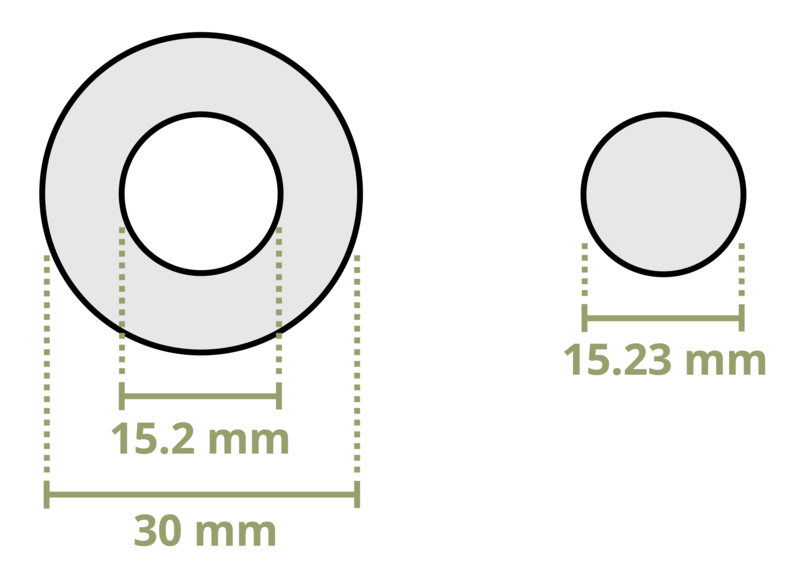
\includegraphics[keepaspectratio]{images/660.png}}\{fig-alt=``Picture
with a coin made of a nickel outter core and a copper inner core. The
nickel is a ring with a outer diameter of 30 mm and an inner diameter of
15.2 mm. The copper is circular with a diameter of 15.23 mm.\}
{[}Problem adapted from © Chris Galitz CC BY NC-SA 4.0{]}

\begin{Shaded}
\begin{Highlighting}[]
\NormalTok{\#| standalone: true}
\NormalTok{\#| viewerHeight: 600}
\NormalTok{\#| components: [viewer]}

\NormalTok{from shiny import App, render, ui, reactive}
\NormalTok{import random}
\NormalTok{import asyncio}
\NormalTok{import io}
\NormalTok{import math}
\NormalTok{import string}
\NormalTok{from datetime import datetime}
\NormalTok{from pathlib import Path}

\NormalTok{def generate\_random\_letters(length):}
\NormalTok{    \# Generate a random string of letters of specified length}
\NormalTok{    return \textquotesingle{}\textquotesingle{}.join(random.choice(string.ascii\_lowercase) for \_ in range(length))  }

\NormalTok{problem\_ID="660"}
\NormalTok{Ti=reactive.Value("\_\_")}
  
\NormalTok{attempts=["Timestamp,Attempt,Answer,Feedback\textbackslash{}n"]}

\NormalTok{app\_ui = ui.page\_fluid(}
\NormalTok{    \#ui.markdown("**Please enter your ID number from your instructor and click to generate your problem**"),}
\NormalTok{    \#ui.input\_text("ID","", placeholder="Enter ID Number Here"),}
\NormalTok{    \#ui.input\_action\_button("generate\_problem", "Generate Problem", class\_="btn{-}primary"),}
\NormalTok{    ui.markdown("**Problem Statement**"),}
\NormalTok{    ui.output\_ui("ui\_problem\_statement"),}
\NormalTok{    ui.input\_text("answer","Your Answer in units of \textbackslash{}u00b0C", placeholder="Please enter your answer"),}
\NormalTok{    ui.input\_action\_button("submit", "Check Answer", class\_="btn{-}primary"),}
\NormalTok{    \#ui.download\_button("download", "Download File to Submit", class\_="btn{-}success"),}
\NormalTok{)}

\NormalTok{def server(input, output, session):}
\NormalTok{    \# Initialize a counter for attempts}
\NormalTok{    attempt\_counter = reactive.Value(0)}

\NormalTok{    @output}
\NormalTok{    @render.ui}
\NormalTok{    def ui\_problem\_statement():}
\NormalTok{        randomize\_vars()}
\NormalTok{        return[ui.markdown(f"A coin is to be made with a nickel outer ring and a copper (α = 17 x 10\textless{}sup\textgreater{}{-}6\textless{}/sup\textgreater{} /°C) core. The dimensions are shown at an initial temperature of \{Ti()\}°C. If the copper is to be cooled to fit inside the nickel, determine the required temperature of the copper.")]}
    
\NormalTok{    \#@reactive.Effect}
\NormalTok{    \#@reactive.event(input.generate\_problem)}
\NormalTok{    def randomize\_vars():}
\NormalTok{        random.seed(101)}
\NormalTok{        Ti.set(random.randrange(10,20,1))}
        
\NormalTok{    @reactive.Effect}
\NormalTok{    @reactive.event(input.submit)}
\NormalTok{    def \_():}
\NormalTok{        attempt\_counter.set(attempt\_counter() + 1)  \# Increment the attempt counter on each submission.}
\NormalTok{        instr= Ti(){-}115.87}
\NormalTok{        if math.isclose(float(input.answer()), instr, rel\_tol=0.01):}
\NormalTok{            check = "*Correct*"}
\NormalTok{            correct\_indicator = "JL"}
\NormalTok{        else:}
\NormalTok{            check = "*Not Correct.*"}
\NormalTok{            correct\_indicator = "JG"}

\NormalTok{        \# Generate random parts for the encoded attempt.}
\NormalTok{        random\_start = generate\_random\_letters(4)}
\NormalTok{        random\_middle = generate\_random\_letters(4)}
\NormalTok{        random\_end = generate\_random\_letters(4)}
\NormalTok{        \#encoded\_attempt = f"\{random\_start\}\{problem\_ID\}{-}\{random\_middle\}\{attempt\_counter()\}\{correct\_indicator\}{-}\{random\_end\}\{input.ID()\}"}

\NormalTok{        \# Store the most recent encoded attempt in a reactive value so it persists across submissions}
\NormalTok{        \#session.encoded\_attempt = reactive.Value(encoded\_attempt)}

\NormalTok{        \# Append the attempt data to the attempts list without the encoded attempt}
\NormalTok{        attempts.append(f"\{datetime.now()\}, \{attempt\_counter()\}, \{input.answer()\}, \{check\}\textbackslash{}n")}

\NormalTok{        \# Show feedback to the user.}
\NormalTok{        feedback = ui.markdown(f"Your answer of \{input.answer()\} is \{check\}.")}
\NormalTok{        m = ui.modal(}
\NormalTok{            feedback,}
\NormalTok{            title="Feedback",}
\NormalTok{            easy\_close=True}
\NormalTok{        )}
\NormalTok{        ui.modal\_show(m)}

\NormalTok{    \#@render.download(filename=lambda: f"Problem\_Log{-}\{problem\_ID\}{-}\{input.ID()\}.csv")}
\NormalTok{    async def download():}
\NormalTok{        \# Start the CSV with the encoded attempt (without label)}
\NormalTok{        final\_encoded = session.encoded\_attempt() if session.encoded\_attempt is not None else "No attempts"}
\NormalTok{        yield f"\{final\_encoded\}\textbackslash{}n\textbackslash{}n"}
        
\NormalTok{        \# Write the header for the remaining CSV data once}
\NormalTok{        yield "Timestamp,Attempt,Answer,Feedback\textbackslash{}n"}
        
\NormalTok{        \# Write the attempts data, ensure that the header from the attempts list is not written again}
\NormalTok{        for attempt in attempts[1:]:  \# Skip the first element which is the header}
\NormalTok{            await asyncio.sleep(0.25)  \# This delay may not be necessary; adjust as needed}
\NormalTok{            yield attempt}

\NormalTok{\# App installation}
\NormalTok{app = App(app\_ui, server)}
\end{Highlighting}
\end{Shaded}

\chapter*{Problem 4.21 - Thermal
Strain}\label{problem-4.21---thermal-strain}
\addcontentsline{toc}{chapter}{Problem 4.21 - Thermal Strain}

\markboth{Problem 4.21 - Thermal Strain}{Problem 4.21 - Thermal Strain}

\pandocbounded{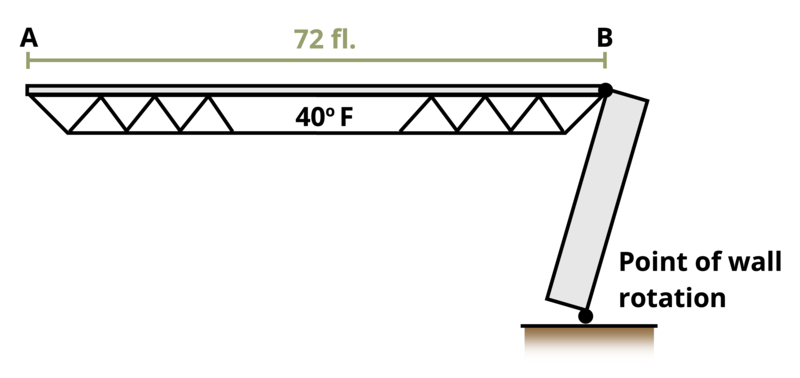
\includegraphics[keepaspectratio]{images/661.png}}
{[}Problem adapted from © Chris Galitz CC BY NC-SA 4.0{]}

\begin{Shaded}
\begin{Highlighting}[]
\NormalTok{\#| standalone: true}
\NormalTok{\#| viewerHeight: 600}
\NormalTok{\#| components: [viewer]}

\NormalTok{from shiny import App, render, ui, reactive}
\NormalTok{import random}
\NormalTok{import asyncio}
\NormalTok{import io}
\NormalTok{import math}
\NormalTok{import string}
\NormalTok{from datetime import datetime}
\NormalTok{from pathlib import Path}

\NormalTok{def generate\_random\_letters(length):}
\NormalTok{    \# Generate a random string of letters of specified length}
\NormalTok{    return \textquotesingle{}\textquotesingle{}.join(random.choice(string.ascii\_lowercase) for \_ in range(length))  }

\NormalTok{problem\_ID="661"}
\NormalTok{L=reactive.Value("\_\_")}
\NormalTok{Ti=reactive.Value("\_\_")}
\NormalTok{Tf=reactive.Value("\_\_")}

\NormalTok{attempts=["Timestamp,Attempt,Answer,Feedback\textbackslash{}n"]}

\NormalTok{app\_ui = ui.page\_fluid(}
\NormalTok{    \#ui.markdown("**Please enter your ID number from your instructor and click to generate your problem**"),}
\NormalTok{    \#ui.input\_text("ID","", placeholder="Enter ID Number Here"),}
\NormalTok{    \#ui.input\_action\_button("generate\_problem", "Generate Problem", class\_="btn{-}primary"),}
\NormalTok{    ui.markdown("**Problem Statement**"),}
\NormalTok{    ui.output\_ui("ui\_problem\_statement"),}
\NormalTok{    ui.input\_text("answer","Your Answer in units of in", placeholder="Please enter your answer"),}
\NormalTok{    ui.input\_action\_button("submit", "Check Answer", class\_="btn{-}primary"),}
\NormalTok{    \#ui.download\_button("download", "Download File to Submit", class\_="btn{-}success"),}
\NormalTok{)}

\NormalTok{def server(input, output, session):}
\NormalTok{    \# Initialize a counter for attempts}
\NormalTok{    attempt\_counter = reactive.Value(0)}

\NormalTok{    @output}
\NormalTok{    @render.ui}
\NormalTok{    def ui\_problem\_statement():}
\NormalTok{        randomize\_vars()}
\NormalTok{        return[ui.markdown(f"A gymnasium roof of length L = \{L()\} ft is supported by open{-}web steel bar joists. They are installed at an ambient temperature of \{Ti()\}°F. On a hot summer day, the roof temperature reaches \{Tf()\}°F. Determine the change in length of the joists. Assume α = 6.5 x 10\textless{}sup\textgreater{}{-}6\textless{}/sup\textgreater{} /°F.")]}
    
\NormalTok{    \#@reactive.Effect}
\NormalTok{    \#@reactive.event(input.generate\_problem)}
\NormalTok{    def randomize\_vars():}
\NormalTok{        random.seed(101)}
\NormalTok{        L.set(random.randrange(50,100,1))}
\NormalTok{        Ti.set(random.randrange(30,50,1))}
\NormalTok{        Tf.set(random.randrange(100,150,1))}
        
\NormalTok{    @reactive.Effect}
\NormalTok{    @reactive.event(input.submit)}
\NormalTok{    def \_():}
\NormalTok{        attempt\_counter.set(attempt\_counter() + 1)  \# Increment the attempt counter on each submission.}
\NormalTok{        instr=6.5*10**{-}6*(Tf(){-}Ti())*L()*12}
\NormalTok{        if math.isclose(float(input.answer()), instr, rel\_tol=0.01):}
\NormalTok{            check = "*Correct*"}
\NormalTok{            correct\_indicator = "JL"}
\NormalTok{        else:}
\NormalTok{            check = "*Not Correct.*"}
\NormalTok{            correct\_indicator = "JG"}

\NormalTok{        \# Generate random parts for the encoded attempt.}
\NormalTok{        random\_start = generate\_random\_letters(4)}
\NormalTok{        random\_middle = generate\_random\_letters(4)}
\NormalTok{        random\_end = generate\_random\_letters(4)}
\NormalTok{        \#encoded\_attempt = f"\{random\_start\}\{problem\_ID\}{-}\{random\_middle\}\{attempt\_counter()\}\{correct\_indicator\}{-}\{random\_end\}\{input.ID()\}"}

\NormalTok{        \# Store the most recent encoded attempt in a reactive value so it persists across submissions}
\NormalTok{        \#session.encoded\_attempt = reactive.Value(encoded\_attempt)}

\NormalTok{        \# Append the attempt data to the attempts list without the encoded attempt}
\NormalTok{        attempts.append(f"\{datetime.now()\}, \{attempt\_counter()\}, \{input.answer()\}, \{check\}\textbackslash{}n")}

\NormalTok{        \# Show feedback to the user.}
\NormalTok{        feedback = ui.markdown(f"Your answer of \{input.answer()\} is \{check\}.")}
\NormalTok{        m = ui.modal(}
\NormalTok{            feedback,}
\NormalTok{            title="Feedback",}
\NormalTok{            easy\_close=True}
\NormalTok{        )}
\NormalTok{        ui.modal\_show(m)}

\NormalTok{    \#@render.download(filename=lambda: f"Problem\_Log{-}\{problem\_ID\}{-}\{input.ID()\}.csv")}
\NormalTok{    async def download():}
\NormalTok{        \# Start the CSV with the encoded attempt (without label)}
\NormalTok{        final\_encoded = session.encoded\_attempt() if session.encoded\_attempt is not None else "No attempts"}
\NormalTok{        yield f"\{final\_encoded\}\textbackslash{}n\textbackslash{}n"}
        
\NormalTok{        \# Write the header for the remaining CSV data once}
\NormalTok{        yield "Timestamp,Attempt,Answer,Feedback\textbackslash{}n"}
        
\NormalTok{        \# Write the attempts data, ensure that the header from the attempts list is not written again}
\NormalTok{        for attempt in attempts[1:]:  \# Skip the first element which is the header}
\NormalTok{            await asyncio.sleep(0.25)  \# This delay may not be necessary; adjust as needed}
\NormalTok{            yield attempt}

\NormalTok{\# App installation}
\NormalTok{app = App(app\_ui, server)}
\end{Highlighting}
\end{Shaded}

\chapter*{Problem 4.23 - Multiaxial Hooke's
Law}\label{problem-4.23---multiaxial-hookes-law}
\addcontentsline{toc}{chapter}{Problem 4.23 - Multiaxial Hooke's Law}

\markboth{Problem 4.23 - Multiaxial Hooke's Law}{Problem 4.23 -
Multiaxial Hooke's Law}

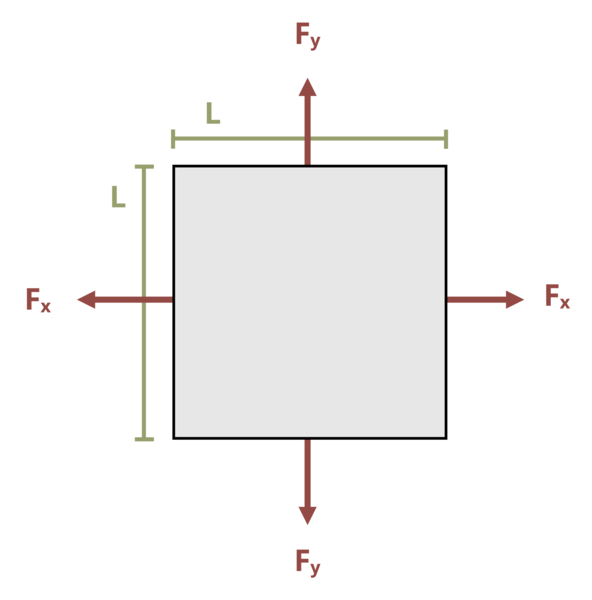
\includegraphics[width=3.125in,height=\textheight,keepaspectratio]{images/204.png}
{[}Problem adapted from © Kurt Gramoll CC BY NC-SA 4.0{]}

\begin{Shaded}
\begin{Highlighting}[]
\NormalTok{\#| standalone: true}
\NormalTok{\#| viewerHeight: 600}
\NormalTok{\#| components: [viewer]}

\NormalTok{from shiny import App, render, ui, reactive}
\NormalTok{import random}
\NormalTok{import asyncio}
\NormalTok{import io}
\NormalTok{import math}
\NormalTok{import string}
\NormalTok{from datetime import datetime}
\NormalTok{from pathlib import Path}

\NormalTok{def generate\_random\_letters(length):}
\NormalTok{    \# Generate a random string of letters of specified length}
\NormalTok{    return \textquotesingle{}\textquotesingle{}.join(random.choice(string.ascii\_lowercase) for \_ in range(length)) }

\NormalTok{problem\_ID="204"}
\NormalTok{L=reactive.Value("\_\_")}
\NormalTok{t=reactive.Value("\_\_")}
\NormalTok{Fx=reactive.Value("\_\_")}
\NormalTok{Fy=reactive.Value("\_\_")}
\NormalTok{E=29000}
\NormalTok{v=0.29}

\NormalTok{attempts=["Timestamp,Attempt,Answer,Feedback\textbackslash{}n"]}

\NormalTok{app\_ui = ui.page\_fluid(}
\NormalTok{    \#ui.markdown("**Please enter your ID number from your instructor and click to generate your problem**"),}
\NormalTok{    \#ui.input\_text("ID","", placeholder="Enter ID Number Here"),}
\NormalTok{    \#ui.input\_action\_button("generate\_problem", "Generate Problem", class\_="btn{-}primary"),}
\NormalTok{    ui.markdown("**Problem Statement**"),}
\NormalTok{    ui.output\_ui("ui\_problem\_statement"),}
\NormalTok{    ui.input\_text("answer","Your Answer in units of inches", placeholder="Please enter your answer"),}
\NormalTok{    ui.input\_action\_button("submit", "Check Answer", class\_="btn{-}primary"),}
\NormalTok{    \#ui.download\_button("download", "Download File to Submit", class\_="btn{-}success"),}
\NormalTok{)}

\NormalTok{def server(input, output, session):}
\NormalTok{    \# Initialize a counter for attempts}
\NormalTok{    attempt\_counter = reactive.Value(0)}

\NormalTok{    @output}
\NormalTok{    @render.ui}
\NormalTok{    def ui\_problem\_statement():}
\NormalTok{        randomize\_vars()}
\NormalTok{        return[ui.markdown(f"A square steel plate of side length L = \{L()\} in. and thickness t = \{t()\} in. is uniformly pulled by two forces F\textless{}sub\textgreater{}x\textless{}/sub\textgreater{} = \{Fx()\} kips and F\textless{}sub\textgreater{}y\textless{}/sub\textgreater{} = \{Fy()\} kips as shown. If E = 29,000 ksi and Poisson\textquotesingle{}s ratio v = 0.29, determine the change in thickness of the plate. ")]}
    
\NormalTok{    \#@reactive.Effect}
\NormalTok{    \#@reactive.event(input.generate\_problem)}
\NormalTok{    def randomize\_vars():}
\NormalTok{        random.seed(101)}
\NormalTok{        L.set(random.randrange(50, 150, 1)/10)}
\NormalTok{        t.set(random.randrange(2, 10, 1)/10)}
\NormalTok{        Fx.set(random.randrange(100, 500, 1)/10)}
\NormalTok{        Fy.set(random.randrange(100, 500, 1)/10)}
        
\NormalTok{    @reactive.Effect}
\NormalTok{    @reactive.event(input.submit)}
\NormalTok{    def \_():}
\NormalTok{        attempt\_counter.set(attempt\_counter() + 1)  \# Increment the attempt counter on each submission.}
\NormalTok{        sigmax = Fx()/(L()*t())}
\NormalTok{        sigmay = Fy()/(L()*t())}
\NormalTok{        instr= t()*({-}v/E)*(sigmax+sigmay)}
\NormalTok{        if math.isclose(float(input.answer()), instr, rel\_tol=0.01):}
\NormalTok{            check = "*Correct*"}
\NormalTok{            correct\_indicator = "JL"}
\NormalTok{        else:}
\NormalTok{            check = "*Not Correct.*"}
\NormalTok{            correct\_indicator = "JG"}

\NormalTok{        \# Generate random parts for the encoded attempt.}
\NormalTok{        random\_start = generate\_random\_letters(4)}
\NormalTok{        random\_middle = generate\_random\_letters(4)}
\NormalTok{        random\_end = generate\_random\_letters(4)}
\NormalTok{        \#encoded\_attempt = f"\{random\_start\}\{problem\_ID\}{-}\{random\_middle\}\{attempt\_counter()\}\{correct\_indicator\}{-}\{random\_end\}\{input.ID()\}"}

\NormalTok{        \# Store the most recent encoded attempt in a reactive value so it persists across submissions}
\NormalTok{        \#session.encoded\_attempt = reactive.Value(encoded\_attempt)}

\NormalTok{        \# Append the attempt data to the attempts list without the encoded attempt}
\NormalTok{        attempts.append(f"\{datetime.now()\}, \{attempt\_counter()\}, \{input.answer()\}, \{check\}\textbackslash{}n")}

\NormalTok{        \# Show feedback to the user.}
\NormalTok{        feedback = ui.markdown(f"Your answer of \{input.answer()\} is \{check\}.")}
\NormalTok{        m = ui.modal(}
\NormalTok{            feedback,}
\NormalTok{            title="Feedback",}
\NormalTok{            easy\_close=True}
\NormalTok{        )}
\NormalTok{        ui.modal\_show(m)}

\NormalTok{    \#@render.download(filename=lambda: f"Problem\_Log{-}\{problem\_ID\}{-}\{input.ID()\}.csv")}
\NormalTok{    async def download():}
\NormalTok{        \# Start the CSV with the encoded attempt (without label)}
\NormalTok{        final\_encoded = session.encoded\_attempt() if session.encoded\_attempt is not None else "No attempts"}
\NormalTok{        yield f"\{final\_encoded\}\textbackslash{}n\textbackslash{}n"}
        
\NormalTok{        \# Write the header for the remaining CSV data once}
\NormalTok{        yield "Timestamp,Attempt,Answer,Feedback\textbackslash{}n"}
        
\NormalTok{        \# Write the attempts data, ensure that the header from the attempts list is not written again}
\NormalTok{        for attempt in attempts[1:]:  \# Skip the first element which is the header}
\NormalTok{            await asyncio.sleep(0.25)  \# This delay may not be necessary; adjust as needed}
\NormalTok{            yield attempt}


\NormalTok{\# App installation}
\NormalTok{app = App(app\_ui, server)}
\end{Highlighting}
\end{Shaded}

\chapter*{Problem 4.24 - Multiaxial Hooke's
Law}\label{problem-4.24---multiaxial-hookes-law}
\addcontentsline{toc}{chapter}{Problem 4.24 - Multiaxial Hooke's Law}

\markboth{Problem 4.24 - Multiaxial Hooke's Law}{Problem 4.24 -
Multiaxial Hooke's Law}

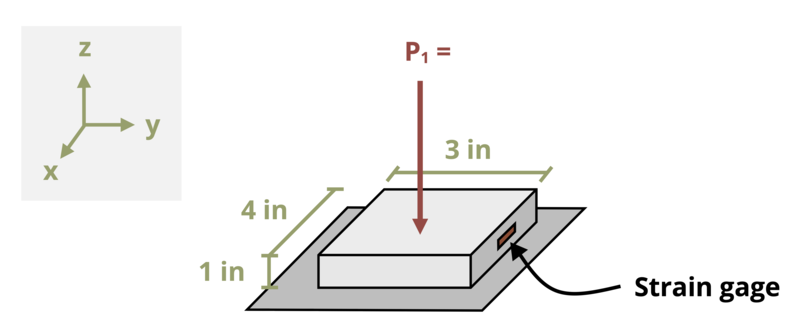
\includegraphics[width=37.44792in,height=\textheight,keepaspectratio]{images/205.png}
{[}Problem adapted from © Kurt Gramoll CC BY NC-SA 4.0{]}

\begin{Shaded}
\begin{Highlighting}[]
\NormalTok{\#| standalone: true}
\NormalTok{\#| viewerHeight: 600}
\NormalTok{\#| components: [viewer]}

\NormalTok{from shiny import App, render, ui, reactive}
\NormalTok{import random}
\NormalTok{import asyncio}
\NormalTok{import io}
\NormalTok{import math}
\NormalTok{import string}
\NormalTok{from datetime import datetime}
\NormalTok{from pathlib import Path}

\NormalTok{def generate\_random\_letters(length):}
\NormalTok{    \# Generate a random string of letters of specified length}
\NormalTok{    return \textquotesingle{}\textquotesingle{}.join(random.choice(string.ascii\_lowercase) for \_ in range(length)) }

\NormalTok{problem\_ID="205"}
\NormalTok{P1=reactive.Value("\_\_")}
\NormalTok{E=reactive.Value("\_\_")}
\NormalTok{v=reactive.Value("\_\_")}
\NormalTok{SG=reactive.Value("\_\_")}

\NormalTok{attempts=["Timestamp,Attempt,Answer,Feedback\textbackslash{}n"]}

\NormalTok{app\_ui = ui.page\_fluid(}
\NormalTok{    \#ui.markdown("**Please enter your ID number from your instructor and click to generate your problem**"),}
\NormalTok{    \#ui.input\_text("ID","", placeholder="Enter ID Number Here"),}
\NormalTok{    \#ui.input\_action\_button("generate\_problem", "Generate Problem", class\_="btn{-}primary"),}
\NormalTok{    ui.markdown("**Problem Statement**"),}
\NormalTok{    ui.output\_ui("ui\_problem\_statement"),}
\NormalTok{    ui.input\_text("answer","Your Answer in percent", placeholder="Please enter your answer"),}
\NormalTok{    ui.input\_action\_button("submit", "Check Answer", class\_="btn{-}primary"),}
\NormalTok{    \#ui.download\_button("download", "Download File to Submit", class\_="btn{-}success"),}
\NormalTok{)}

\NormalTok{def server(input, output, session):}
\NormalTok{    \# Initialize a counter for attempts}
\NormalTok{    attempt\_counter = reactive.Value(0)}

\NormalTok{    @output}
\NormalTok{    @render.ui}
\NormalTok{    def ui\_problem\_statement():}
\NormalTok{        randomize\_vars()}
\NormalTok{        return[ui.markdown(f"A strain gauge is placed on a polymer test sample with an elastic modulus E =  \{E()\} x 10\textless{}sup\textgreater{}6\textless{}/sup\textgreater{} psi and a Poisson\textquotesingle{}s ratio of v = \{v()\}. When a P\textless{}sub\textgreater{}1\textless{}/sub\textgreater{} = \{P1()\} kip vertical load is applied to the test sample, the strain gauge reads a strain of ε = \{SG()\} x 10\textless{}sup\textgreater{}{-}6\textless{}/sup\textgreater{} in the x{-}direction. What is the relative error of the strain gauge compared to the theoretical strain of the test sample? Note: relative error is defined to be the difference between the measured value and the theoretical value divided by the theoretical value.")]}
    
\NormalTok{    \#@reactive.Effect}
\NormalTok{    \#@reactive.event(input.generate\_problem)}
\NormalTok{    def randomize\_vars():}
\NormalTok{        random.seed(101)}
\NormalTok{        P1.set(random.randrange(20, 200, 1)/10)}
\NormalTok{        E.set(random.randrange(5, 20, 1))}
\NormalTok{        v.set(random.randrange(20, 40, 1)/100)}
\NormalTok{        SG.set(round((v()*P1()*1000)/(12*E()),1){-}(random.randrange(3, 20, 1)/10))}
        
\NormalTok{    @reactive.Effect}
\NormalTok{    @reactive.event(input.submit)}
\NormalTok{    def \_():}
\NormalTok{        attempt\_counter.set(attempt\_counter() + 1)  \# Increment the attempt counter on each submission.}
\NormalTok{        sigmaz = ({-}P1()*1000)/(4*3)}
\NormalTok{        Ex = (({-}v()*(sigmaz))/(E()*10**6))}
\NormalTok{        instr=  ((Ex {-} SG()*10**{-}6)/Ex)*100}
\NormalTok{        if math.isclose(float(input.answer()), instr, rel\_tol=0.01):}
\NormalTok{            check = "*Correct*"}
\NormalTok{            correct\_indicator = "JL"}
\NormalTok{        else:}
\NormalTok{            check = "*Not Correct.*"}
\NormalTok{            correct\_indicator = "JG"}

\NormalTok{        \# Generate random parts for the encoded attempt.}
\NormalTok{        random\_start = generate\_random\_letters(4)}
\NormalTok{        random\_middle = generate\_random\_letters(4)}
\NormalTok{        random\_end = generate\_random\_letters(4)}
\NormalTok{        \#encoded\_attempt = f"\{random\_start\}\{problem\_ID\}{-}\{random\_middle\}\{attempt\_counter()\}\{correct\_indicator\}{-}\{random\_end\}\{input.ID()\}"}

\NormalTok{        \# Store the most recent encoded attempt in a reactive value so it persists across submissions}
\NormalTok{        \#session.encoded\_attempt = reactive.Value(encoded\_attempt)}

\NormalTok{        \# Append the attempt data to the attempts list without the encoded attempt}
\NormalTok{        attempts.append(f"\{datetime.now()\}, \{attempt\_counter()\}, \{input.answer()\}, \{check\}\textbackslash{}n")}

\NormalTok{        \# Show feedback to the user.}
\NormalTok{        feedback = ui.markdown(f"Your answer of \{input.answer()\} is \{check\}.")}
\NormalTok{        m = ui.modal(}
\NormalTok{            feedback,}
\NormalTok{            title="Feedback",}
\NormalTok{            easy\_close=True}
\NormalTok{        )}
\NormalTok{        ui.modal\_show(m)}

\NormalTok{    \#@render.download(filename=lambda: f"Problem\_Log{-}\{problem\_ID\}{-}\{input.ID()\}.csv")}
\NormalTok{    async def download():}
\NormalTok{        \# Start the CSV with the encoded attempt (without label)}
\NormalTok{        final\_encoded = session.encoded\_attempt() if session.encoded\_attempt is not None else "No attempts"}
\NormalTok{        yield f"\{final\_encoded\}\textbackslash{}n\textbackslash{}n"}
        
\NormalTok{        \# Write the header for the remaining CSV data once}
\NormalTok{        yield "Timestamp,Attempt,Answer,Feedback\textbackslash{}n"}
        
\NormalTok{        \# Write the attempts data, ensure that the header from the attempts list is not written again}
\NormalTok{        for attempt in attempts[1:]:  \# Skip the first element which is the header}
\NormalTok{            await asyncio.sleep(0.25)  \# This delay may not be necessary; adjust as needed}
\NormalTok{            yield attempt}

\NormalTok{\# App installation}
\NormalTok{app = App(app\_ui, server)}
\end{Highlighting}
\end{Shaded}

\chapter*{Problem 4.25 - Multiaxial Hooke's
Law}\label{problem-4.25---multiaxial-hookes-law}
\addcontentsline{toc}{chapter}{Problem 4.25 - Multiaxial Hooke's Law}

\markboth{Problem 4.25 - Multiaxial Hooke's Law}{Problem 4.25 -
Multiaxial Hooke's Law}

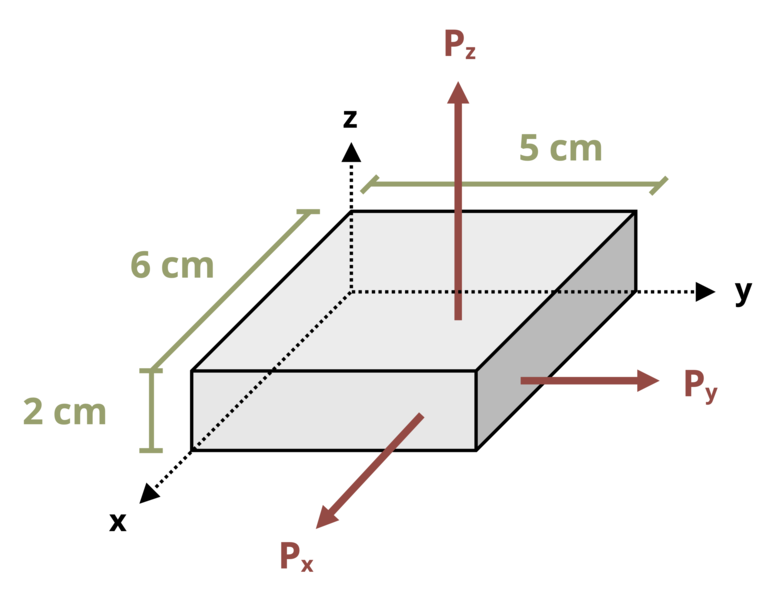
\includegraphics[width=20.40625in,height=\textheight,keepaspectratio]{images/208.png}
{[}Problem adapted from © Kurt Gramoll CC BY NC-SA 4.0{]}

\begin{Shaded}
\begin{Highlighting}[]
\NormalTok{\#| standalone: true}
\NormalTok{\#| viewerHeight: 600}
\NormalTok{\#| components: [viewer]}

\NormalTok{from shiny import App, render, ui, reactive}
\NormalTok{import random}
\NormalTok{import asyncio}
\NormalTok{import io}
\NormalTok{import math}
\NormalTok{import string}
\NormalTok{from datetime import datetime}
\NormalTok{from pathlib import Path}

\NormalTok{def generate\_random\_letters(length):}
\NormalTok{    \# Generate a random string of letters of specified length}
\NormalTok{    return \textquotesingle{}\textquotesingle{}.join(random.choice(string.ascii\_lowercase) for \_ in range(length)) }

\NormalTok{problem\_ID="208"}
\NormalTok{Px=reactive.Value("\_\_")}
\NormalTok{Py=reactive.Value("\_\_")}
\NormalTok{Pz=reactive.Value("\_\_")}
\NormalTok{L=reactive.Value("\_\_")}
\NormalTok{E=reactive.Value("\_\_")}
\NormalTok{v=reactive.Value("\_\_")}


\NormalTok{attempts=["Timestamp,Attempt,Answer,Feedback\textbackslash{}n"]}

\NormalTok{app\_ui = ui.page\_fluid(}
\NormalTok{    \#ui.markdown("**Please enter your ID number from your instructor and click to generate your problem**"),}
\NormalTok{    \#ui.input\_text("ID","", placeholder="Enter ID Number Here"),}
\NormalTok{    \#ui.input\_action\_button("generate\_problem", "Generate Problem", class\_="btn{-}primary"),}
\NormalTok{    ui.markdown("**Problem Statement**"),}
\NormalTok{    ui.output\_ui("ui\_problem\_statement"),}
\NormalTok{    ui.input\_text("answer","Your Answer in percent", placeholder="Please enter your answer"),}
\NormalTok{    ui.input\_action\_button("submit", "Check Answer", class\_="btn{-}primary"),}
\NormalTok{    \#ui.download\_button("download", "Download File to Submit", class\_="btn{-}success"),}
\NormalTok{)}


\NormalTok{def server(input, output, session):}
\NormalTok{    \# Initialize a counter for attempts}
\NormalTok{    attempt\_counter = reactive.Value(0)}

\NormalTok{    @output}
\NormalTok{    @render.ui}
\NormalTok{    def ui\_problem\_statement():}
\NormalTok{        randomize\_vars()}
\NormalTok{        return[ui.markdown(f"A block is pulled in all three directions (P\textless{}sub\textgreater{}x\textless{}/sub\textgreater{} = \{Px()\} kN, P\textless{}sub\textgreater{}y\textless{}/sub\textgreater{} = \{Py()\} kN, P\textless{}sub\textgreater{}z\textless{}/sub\textgreater{} = \{Pz()\} kN). What is the percent change in volume after all three loads are applied? Assume E = \{E()\} MPa and v = \{v()\}. ")]}
    
\NormalTok{    \#@reactive.Effect}
\NormalTok{    \#@reactive.event(input.generate\_problem)}
\NormalTok{    def randomize\_vars():}
\NormalTok{        random.seed(101)}
\NormalTok{        Px.set(random.randrange(1, 20, 1))}
\NormalTok{        Py.set(random.randrange(1, 20, 1))}
\NormalTok{        Pz.set(random.randrange(1, 20, 1))}
\NormalTok{        E.set(random.randrange(1000, 2000, 100))}
\NormalTok{        v.set(random.randrange(20, 40, 1)/100)}
        
\NormalTok{    @reactive.Effect}
\NormalTok{    @reactive.event(input.submit)}
\NormalTok{    def \_():}
\NormalTok{        attempt\_counter.set(attempt\_counter() + 1)  \# Increment the attempt counter on each submission.}
\NormalTok{        sigmax = (Px()/(5*2))*10}
\NormalTok{        sigmay = (Py()/(6*2))*10}
\NormalTok{        sigmaz = (Pz()/(5*6))*10}
\NormalTok{        Ex = (sigmax {-} v()*(sigmay+sigmaz))/(E())}
\NormalTok{        Ey = (sigmay {-} v()*(sigmaz+sigmax))/(E())}
\NormalTok{        Ez = (sigmaz {-} v()*(sigmax+sigmay))/(E())}
\NormalTok{        Lx = 6 + 6*Ex}
\NormalTok{        Ly = 5 + 5*Ey}
\NormalTok{        Lz = 2 + 2*Ez}
\NormalTok{        instr= (((Lx*Ly*Lz){-}60)/60)*100}
\NormalTok{        if math.isclose(float(input.answer()), instr, rel\_tol=0.01):}
\NormalTok{            check = "*Correct*"}
\NormalTok{            correct\_indicator = "JL"}
\NormalTok{        else:}
\NormalTok{            check = "*Not Correct.*"}
\NormalTok{            correct\_indicator = "JG"}

\NormalTok{        \# Generate random parts for the encoded attempt.}
\NormalTok{        random\_start = generate\_random\_letters(4)}
\NormalTok{        random\_middle = generate\_random\_letters(4)}
\NormalTok{        random\_end = generate\_random\_letters(4)}
\NormalTok{        \#encoded\_attempt = f"\{random\_start\}\{problem\_ID\}{-}\{random\_middle\}\{attempt\_counter()\}\{correct\_indicator\}{-}\{random\_end\}\{input.ID()\}"}

\NormalTok{        \# Store the most recent encoded attempt in a reactive value so it persists across submissions}
\NormalTok{        \#session.encoded\_attempt = reactive.Value(encoded\_attempt)}

\NormalTok{        \# Append the attempt data to the attempts list without the encoded attempt}
\NormalTok{        attempts.append(f"\{datetime.now()\}, \{attempt\_counter()\}, \{input.answer()\}, \{check\}\textbackslash{}n")}

\NormalTok{        \# Show feedback to the user.}
\NormalTok{        feedback = ui.markdown(f"Your answer of \{input.answer()\} is \{check\}.")}
\NormalTok{        m = ui.modal(}
\NormalTok{            feedback,}
\NormalTok{            title="Feedback",}
\NormalTok{            easy\_close=True}
\NormalTok{        )}
\NormalTok{        ui.modal\_show(m)}

\NormalTok{    \#@render.download(filename=lambda: f"Problem\_Log{-}\{problem\_ID\}{-}\{input.ID()\}.csv")}
\NormalTok{    async def download():}
\NormalTok{        \# Start the CSV with the encoded attempt (without label)}
\NormalTok{        final\_encoded = session.encoded\_attempt() if session.encoded\_attempt is not None else "No attempts"}
\NormalTok{        yield f"\{final\_encoded\}\textbackslash{}n\textbackslash{}n"}
        
\NormalTok{        \# Write the header for the remaining CSV data once}
\NormalTok{        yield "Timestamp,Attempt,Answer,Feedback\textbackslash{}n"}
        
\NormalTok{        \# Write the attempts data, ensure that the header from the attempts list is not written again}
\NormalTok{        for attempt in attempts[1:]:  \# Skip the first element which is the header}
\NormalTok{            await asyncio.sleep(0.25)  \# This delay may not be necessary; adjust as needed}
\NormalTok{            yield attempt}


\NormalTok{\# App installation}
\NormalTok{app = App(app\_ui, server)}
\end{Highlighting}
\end{Shaded}

\chapter*{Problem 4.26 - Multiaxial Hooke's
Law}\label{problem-4.26---multiaxial-hookes-law}
\addcontentsline{toc}{chapter}{Problem 4.26 - Multiaxial Hooke's Law}

\markboth{Problem 4.26 - Multiaxial Hooke's Law}{Problem 4.26 -
Multiaxial Hooke's Law}

\pandocbounded{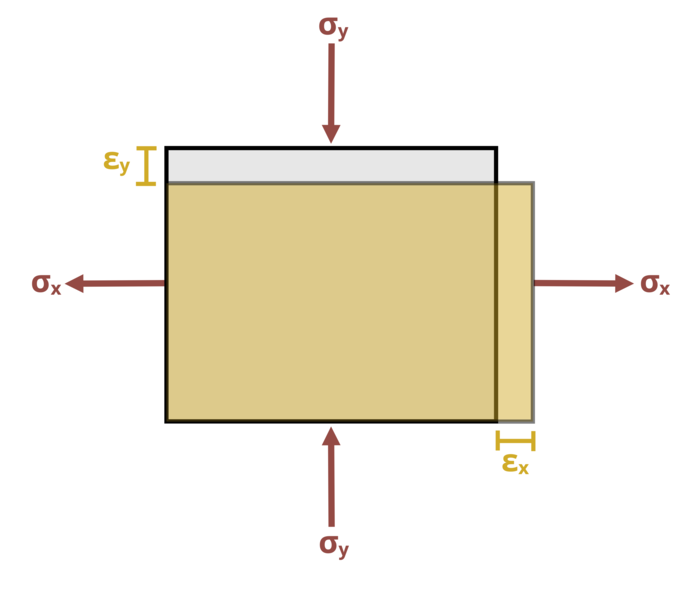
\includegraphics[keepaspectratio]{images/209.png}}
{[}Problem adapted from © Kurt Gramoll CC BY NC-SA 4.0{]}

\begin{Shaded}
\begin{Highlighting}[]
\NormalTok{\#| standalone: true}
\NormalTok{\#| viewerHeight: 600}
\NormalTok{\#| components: [viewer]}

\NormalTok{from shiny import App, render, ui, reactive}
\NormalTok{import random}
\NormalTok{import asyncio}
\NormalTok{import io}
\NormalTok{import math}
\NormalTok{import string}
\NormalTok{from datetime import datetime}
\NormalTok{from pathlib import Path}

\NormalTok{def generate\_random\_letters(length):}
\NormalTok{    \# Generate a random string of letters of specified length}
\NormalTok{    return \textquotesingle{}\textquotesingle{}.join(random.choice(string.ascii\_lowercase) for \_ in range(length))  }

\NormalTok{problem\_ID="209"}
\NormalTok{sigma\_x=reactive.Value("\_\_")}
\NormalTok{sigma\_y=reactive.Value("\_\_")}
\NormalTok{e\_x=reactive.Value("\_\_")}
\NormalTok{e\_y=reactive.Value("\_\_")}
\NormalTok{placeholder = reactive.Value("\_\_")}
  
\NormalTok{attempts=["Timestamp,Attempt,Answer,Feedback\textbackslash{}n"]}

\NormalTok{app\_ui = ui.page\_fluid(}
\NormalTok{    \#ui.markdown("**Please enter your ID number from your instructor and click to generate your problem**"),}
\NormalTok{    \#ui.input\_text("ID","", placeholder="Enter ID Number Here"),}
\NormalTok{    \#ui.input\_action\_button("generate\_problem", "Generate Problem", class\_="btn{-}primary"),}
\NormalTok{    ui.markdown("**Problem Statement**"),}
\NormalTok{    ui.output\_ui("ui\_problem\_statement"),}
\NormalTok{    ui.input\_text("answer","Your Answer", placeholder="Please enter your answer"),}
\NormalTok{    ui.input\_action\_button("submit", "Check Answer", class\_="btn{-}primary"),}
\NormalTok{    \#ui.download\_button("download", "Download File to Submit", class\_="btn{-}success"),}
\NormalTok{)}

\NormalTok{def server(input, output, session):}
\NormalTok{    \# Initialize a counter for attempts}
\NormalTok{    attempt\_counter = reactive.Value(0)}

\NormalTok{    @output}
\NormalTok{    @render.ui}
\NormalTok{    def ui\_problem\_statement():}
\NormalTok{        randomize\_vars()}
\NormalTok{        return[ui.markdown(f"Pressure loading is applied to a plate in both the x and y directions, and the strains are recorded using strain gages. If stresses σ\textless{}sub\textgreater{}x\textless{}/sub\textgreater{} = \{sigma\_x()\} ksi, σ\textless{}sub\textgreater{}y\textless{}/sub\textgreater{} = \{sigma\_y()\} ksi, and strains ε\textless{}sub\textgreater{}x\textless{}/sub\textgreater{} = \{e\_x()\} µ and ε\textless{}sub\textgreater{}y\textless{}/sub\textgreater{} = \{e\_y()\} µ, calculate Poisson\textquotesingle{}s ratio for the material.")]}
    
\NormalTok{    \#@reactive.Effect}
\NormalTok{    \#@reactive.event(input.generate\_problem)}
\NormalTok{    def randomize\_vars():}
\NormalTok{        random.seed(101)}
\NormalTok{        sigma\_x.set(random.randrange(5, 20, 1))}
\NormalTok{        sigma\_y.set(random.randrange(5, 20, 1))}
\NormalTok{        e\_x.set(random.randrange(2100, 2500, 10))}
\NormalTok{        placeholder.set(random.randrange(15,40,1)/100)}
\NormalTok{        e\_y.set(round(e\_x()*(sigma\_y(){-}placeholder()*sigma\_x())/(sigma\_x()+placeholder()*{-}sigma\_y())))}
        
\NormalTok{    @reactive.Effect}
\NormalTok{    @reactive.event(input.submit)}
\NormalTok{    def \_():}
\NormalTok{        attempt\_counter.set(attempt\_counter() + 1)  \# Increment the attempt counter on each submission.}
        
\NormalTok{        instr= {-}(sigma\_x()/e\_x()+sigma\_y()/{-}e\_y())/({-}sigma\_y()/e\_x(){-}sigma\_x()/{-}e\_y())}
\NormalTok{        if math.isclose(float(input.answer()), instr, rel\_tol=0.01):}
\NormalTok{            check = "*Correct*"}
\NormalTok{            correct\_indicator = "JL"}
\NormalTok{        else:}
\NormalTok{            check = "*Not Correct.*"}
\NormalTok{            correct\_indicator = "JG"}

\NormalTok{        \# Generate random parts for the encoded attempt.}
\NormalTok{        random\_start = generate\_random\_letters(4)}
\NormalTok{        random\_middle = generate\_random\_letters(4)}
\NormalTok{        random\_end = generate\_random\_letters(4)}
\NormalTok{        \#encoded\_attempt = f"\{random\_start\}\{problem\_ID\}{-}\{random\_middle\}\{attempt\_counter()\}\{correct\_indicator\}{-}\{random\_end\}\{input.ID()\}"}

\NormalTok{        \# Store the most recent encoded attempt in a reactive value so it persists across submissions}
\NormalTok{        \#session.encoded\_attempt = reactive.Value(encoded\_attempt)}

\NormalTok{        \# Append the attempt data to the attempts list without the encoded attempt}
\NormalTok{        attempts.append(f"\{datetime.now()\}, \{attempt\_counter()\}, \{input.answer()\}, \{check\}\textbackslash{}n")}

\NormalTok{        \# Show feedback to the user.}
\NormalTok{        feedback = ui.markdown(f"Your answer of \{input.answer()\} is \{check\}.")}
\NormalTok{        m = ui.modal(}
\NormalTok{            feedback,}
\NormalTok{            title="Feedback",}
\NormalTok{            easy\_close=True}
\NormalTok{        )}
\NormalTok{        ui.modal\_show(m)}

\NormalTok{    \#@render.download(filename=lambda: f"Problem\_Log{-}\{problem\_ID\}{-}\{input.ID()\}.csv")}
\NormalTok{    async def download():}
\NormalTok{        \# Start the CSV with the encoded attempt (without label)}
\NormalTok{        final\_encoded = session.encoded\_attempt() if session.encoded\_attempt is not None else "No attempts"}
\NormalTok{        yield f"\{final\_encoded\}\textbackslash{}n\textbackslash{}n"}
        
\NormalTok{        \# Write the header for the remaining CSV data once}
\NormalTok{        yield "Timestamp,Attempt,Answer,Feedback\textbackslash{}n"}
        
\NormalTok{        \# Write the attempts data, ensure that the header from the attempts list is not written again}
\NormalTok{        for attempt in attempts[1:]:  \# Skip the first element which is the header}
\NormalTok{            await asyncio.sleep(0.25)  \# This delay may not be necessary; adjust as needed}
\NormalTok{            yield attempt}

\NormalTok{\# App installation}
\NormalTok{app = App(app\_ui, server)}
\end{Highlighting}
\end{Shaded}

\chapter*{Problem 4.27 - Multiaxial Hooke's
Law}\label{problem-4.27---multiaxial-hookes-law}
\addcontentsline{toc}{chapter}{Problem 4.27 - Multiaxial Hooke's Law}

\markboth{Problem 4.27 - Multiaxial Hooke's Law}{Problem 4.27 -
Multiaxial Hooke's Law}

\pandocbounded{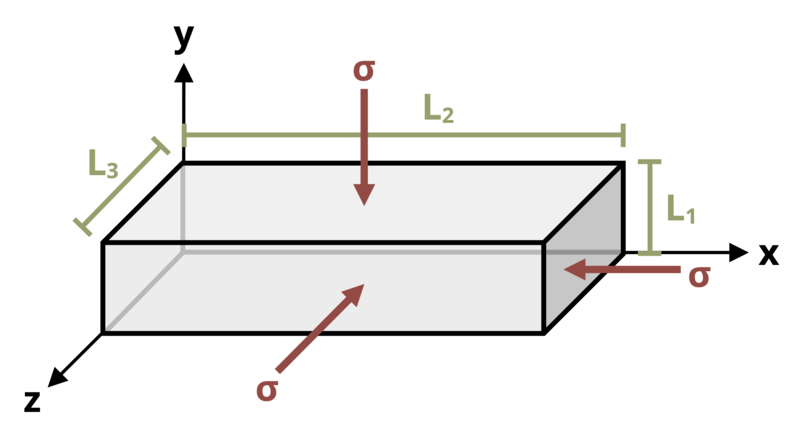
\includegraphics[keepaspectratio]{images/210.png}}
{[}Problem adapted from © Kurt Gramoll CC BY NC-SA 4.0{]}

\begin{Shaded}
\begin{Highlighting}[]
\NormalTok{\#| standalone: true}
\NormalTok{\#| viewerHeight: 600}
\NormalTok{\#| components: [viewer]}

\NormalTok{from shiny import App, render, ui, reactive}
\NormalTok{import random}
\NormalTok{import asyncio}
\NormalTok{import io}
\NormalTok{import math}
\NormalTok{import string}
\NormalTok{from datetime import datetime}
\NormalTok{from pathlib import Path}

\NormalTok{def generate\_random\_letters(length):}
\NormalTok{    \# Generate a random string of letters of specified length}
\NormalTok{    return \textquotesingle{}\textquotesingle{}.join(random.choice(string.ascii\_lowercase) for \_ in range(length))}

\NormalTok{problem\_ID="210"}
\NormalTok{x=reactive.Value("\_\_")}
\NormalTok{E=reactive.Value("\_\_")}
\NormalTok{v=reactive.Value("\_\_")}
  
\NormalTok{attempts=["Timestamp,Attempt,Answer,Feedback\textbackslash{}n"]}

\NormalTok{app\_ui = ui.page\_fluid(}
\NormalTok{    \#ui.markdown("**Please enter your ID number from your instructor and click to generate your problem**"),}
\NormalTok{    \#ui.input\_text("ID","", placeholder="Enter ID Number Here"),}
\NormalTok{    \#ui.input\_action\_button("generate\_problem", "Generate Problem", class\_="btn{-}primary"),}
\NormalTok{    ui.markdown("**Problem Statement**"),}
\NormalTok{    ui.output\_ui("ui\_problem\_statement"),}
\NormalTok{    ui.input\_text("answer","Your Answer in units of MPa", placeholder="Please enter your answer"),}
\NormalTok{    ui.input\_action\_button("submit", "Check Answer", class\_="btn{-}primary"),}
\NormalTok{    \#ui.download\_button("download", "Download File to Submit", class\_="btn{-}success"),}
\NormalTok{)}

\NormalTok{def server(input, output, session):}
\NormalTok{    \# Initialize a counter for attempts}
\NormalTok{    attempt\_counter = reactive.Value(0)}

\NormalTok{    @output}
\NormalTok{    @render.ui}
\NormalTok{    def ui\_problem\_statement():}
\NormalTok{        randomize\_vars()}
\NormalTok{        return[ui.markdown(f"A rigid block is subjected to uniform hydrostatic pressure, σ, on all surfaces. It is noted that the block contracts in the x{-}direction by \{x()\} x 10\textless{}sup\textgreater{}{-}3\textless{}/sup\textgreater{} cm when the pressure is applied. If E = \{E()\} GPa and ν = \{v()\}, determine the magnitude of the applied pressure. Let L\textless{}sub\textgreater{}1\textless{}/sub\textgreater{} = 5 cm, L\textless{}sub\textgreater{}2\textless{}/sub\textgreater{} = 30 cm, and L\textless{}sub\textgreater{}3\textless{}/sub\textgreater{} = 15 cm.")]}
    
\NormalTok{    \#@reactive.Effect}
\NormalTok{    \#@reactive.event(input.generate\_problem)}
\NormalTok{    def randomize\_vars():}
\NormalTok{        random.seed(101)}
\NormalTok{        x.set(random.randrange(15,100,1)/10)}
\NormalTok{        E.set(random.randrange(75,150,1))}
\NormalTok{        v.set(random.randrange(20,40,1)/100)}
        
\NormalTok{    @reactive.Effect}
\NormalTok{    @reactive.event(input.submit)}
\NormalTok{    def \_():}
\NormalTok{        attempt\_counter.set(attempt\_counter() + 1)  \# Increment the attempt counter on each submission.}
    
\NormalTok{        instr= x()/30*E()/(1{-}2*v())}
\NormalTok{        if math.isclose(float(input.answer()), instr, rel\_tol=0.01):}
\NormalTok{            check = "*Correct*"}
\NormalTok{            correct\_indicator = "JL"}
\NormalTok{        else:}
\NormalTok{            check = "*Not Correct.*"}
\NormalTok{            correct\_indicator = "JG"}

\NormalTok{        \# Generate random parts for the encoded attempt.}
\NormalTok{        random\_start = generate\_random\_letters(4)}
\NormalTok{        random\_middle = generate\_random\_letters(4)}
\NormalTok{        random\_end = generate\_random\_letters(4)}
\NormalTok{        \#encoded\_attempt = f"\{random\_start\}\{problem\_ID\}{-}\{random\_middle\}\{attempt\_counter()\}\{correct\_indicator\}{-}\{random\_end\}\{input.ID()\}"}

\NormalTok{        \# Store the most recent encoded attempt in a reactive value so it persists across submissions}
\NormalTok{        \#session.encoded\_attempt = reactive.Value(encoded\_attempt)}

\NormalTok{        \# Append the attempt data to the attempts list without the encoded attempt}
\NormalTok{        attempts.append(f"\{datetime.now()\}, \{attempt\_counter()\}, \{input.answer()\}, \{check\}\textbackslash{}n")}

\NormalTok{        \# Show feedback to the user.}
\NormalTok{        feedback = ui.markdown(f"Your answer of \{input.answer()\} is \{check\}.")}
\NormalTok{        m = ui.modal(}
\NormalTok{            feedback,}
\NormalTok{            title="Feedback",}
\NormalTok{            easy\_close=True}
\NormalTok{        )}
\NormalTok{        ui.modal\_show(m)}

\NormalTok{    \#@render.download(filename=lambda: f"Problem\_Log{-}\{problem\_ID\}{-}\{input.ID()\}.csv")}
\NormalTok{    async def download():}
\NormalTok{        \# Start the CSV with the encoded attempt (without label)}
\NormalTok{        final\_encoded = session.encoded\_attempt() if session.encoded\_attempt is not None else "No attempts"}
\NormalTok{        yield f"\{final\_encoded\}\textbackslash{}n\textbackslash{}n"}
        
\NormalTok{        \# Write the header for the remaining CSV data once}
\NormalTok{        yield "Timestamp,Attempt,Answer,Feedback\textbackslash{}n"}
        
\NormalTok{        \# Write the attempts data, ensure that the header from the attempts list is not written again}
\NormalTok{        for attempt in attempts[1:]:  \# Skip the first element which is the header}
\NormalTok{            await asyncio.sleep(0.25)  \# This delay may not be necessary; adjust as needed}
\NormalTok{            yield attempt}


\NormalTok{\# App installation}
\NormalTok{app = App(app\_ui, server)}
\end{Highlighting}
\end{Shaded}

\chapter*{Problem 4.28 - Multiaxial Hooke's
Law}\label{problem-4.28---multiaxial-hookes-law}
\addcontentsline{toc}{chapter}{Problem 4.28 - Multiaxial Hooke's Law}

\markboth{Problem 4.28 - Multiaxial Hooke's Law}{Problem 4.28 -
Multiaxial Hooke's Law}

\pandocbounded{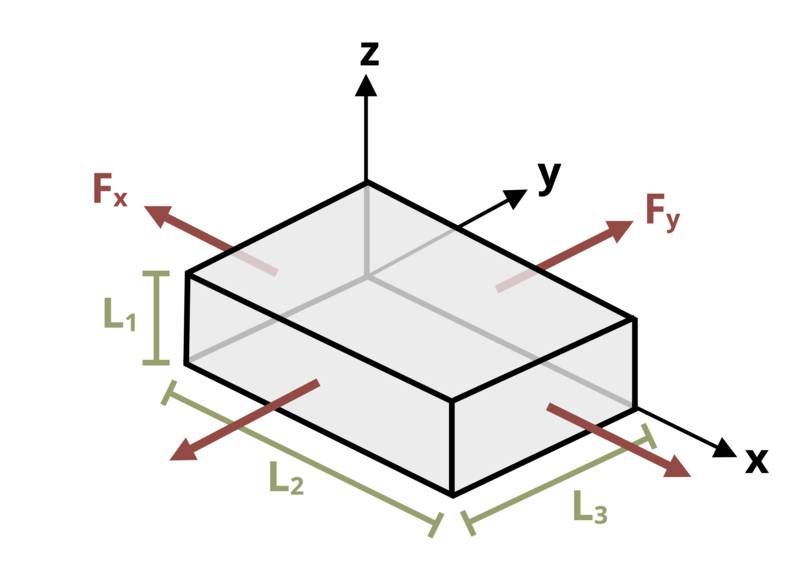
\includegraphics[keepaspectratio]{images/211.png}}
{[}Problem adapted from © Kurt Gramoll CC BY NC-SA 4.0{]}

\begin{Shaded}
\begin{Highlighting}[]
\NormalTok{\#| standalone: true}
\NormalTok{\#| viewerHeight: 600}
\NormalTok{\#| components: [viewer]}

\NormalTok{from shiny import App, render, ui, reactive}
\NormalTok{import random}
\NormalTok{import asyncio}
\NormalTok{import io}
\NormalTok{import math}
\NormalTok{import string}
\NormalTok{from datetime import datetime}
\NormalTok{from pathlib import Path}

\NormalTok{def generate\_random\_letters(length):}
\NormalTok{    \# Generate a random string of letters of specified length}
\NormalTok{    return \textquotesingle{}\textquotesingle{}.join(random.choice(string.ascii\_lowercase) for \_ in range(length))}

\NormalTok{problem\_ID="211"}
\NormalTok{Fx=reactive.Value("\_\_")}
\NormalTok{Fy=reactive.Value("\_\_")}
\NormalTok{E=reactive.Value("\_\_")}
\NormalTok{v=reactive.Value("\_\_")}
  
\NormalTok{attempts=["Timestamp,Attempt,Answer,Feedback\textbackslash{}n"]}

\NormalTok{app\_ui = ui.page\_fluid(}
\NormalTok{    \#ui.markdown("**Please enter your ID number from your instructor and click to generate your problem**"),}
\NormalTok{    \#ui.input\_text("ID","", placeholder="Enter ID Number Here"),}
\NormalTok{    \#ui.input\_action\_button("generate\_problem", "Generate Problem", class\_="btn{-}primary"),}
\NormalTok{    ui.markdown("**Problem Statement**"),}
\NormalTok{    ui.output\_ui("ui\_problem\_statement"),}
\NormalTok{    ui.input\_text("answer","Your Answer in units of in\textbackslash{}u00B3", placeholder="Please enter your answer"),}
\NormalTok{    ui.input\_action\_button("submit", "Check Answer", class\_="btn{-}primary"),}
\NormalTok{    \#ui.download\_button("download", "Download File to Submit", class\_="btn{-}success"),}
\NormalTok{)}

\NormalTok{def server(input, output, session):}
\NormalTok{    \# Initialize a counter for attempts}
\NormalTok{    attempt\_counter = reactive.Value(0)}

\NormalTok{    @output}
\NormalTok{    @render.ui}
\NormalTok{    def ui\_problem\_statement():}
\NormalTok{        randomize\_vars()}
\NormalTok{        return[ui.markdown(f"A rectangular block is pulled in two directions. Determine the total change in volume. Assume force F\textless{}sub\textgreater{}x\textless{}/sub\textgreater{} = \{Fx()\} kips, force F\textless{}sub\textgreater{}y\textless{}/sub\textgreater{} = \{Fy()\} kips, E = \{E()\} x 10\textless{}sup\textgreater{}6\textless{}/sup\textgreater{} psi, and ν = \{v()\}. Let L\textless{}sub\textgreater{}1\textless{}/sub\textgreater{} = 0.5 in, L\textless{}sub\textgreater{}2\textless{}/sub\textgreater{} = 10 in, and L\textless{}sub\textgreater{}3\textless{}/sub\textgreater{} = 8 in.")]}
    
\NormalTok{    \#@reactive.Effect}
\NormalTok{    \#@reactive.event(input.generate\_problem)}
\NormalTok{    def randomize\_vars():}
\NormalTok{        random.seed(101)}
\NormalTok{        Fx.set(random.randrange(50,200,1)/10)}
\NormalTok{        Fy.set(random.randrange(50,200,1)/10)}
\NormalTok{        E.set(random.randrange(75,150,1)/10)}
\NormalTok{        v.set(random.randrange(20,40,1)/100)}
        
\NormalTok{    @reactive.Effect}
\NormalTok{    @reactive.event(input.submit)}
\NormalTok{    def \_():}
\NormalTok{        attempt\_counter.set(attempt\_counter() + 1)  \# Increment the attempt counter on each submission.}
\NormalTok{        sigmax = Fx()/4}
\NormalTok{        sigmay=Fy()/5}
\NormalTok{        strainx = (sigmax{-}v()*sigmay)/(E()*1000)}
\NormalTok{        strainy = (sigmay{-}v()*sigmax)/(E()*1000)}
\NormalTok{        strainz = ({-}v()*(sigmax+sigmay))/(E()*1000)}
\NormalTok{        LxN = 10+10*strainx}
\NormalTok{        LyN = 8+8*strainy}
\NormalTok{        LzN = 0.5+0.5*strainz}
\NormalTok{        VN = LxN*LyN*LzN}
\NormalTok{        Vo = 10*8*0.5}
\NormalTok{        instr= VN{-}Vo}
\NormalTok{        if math.isclose(float(input.answer()), instr, rel\_tol=0.01):}
\NormalTok{            check = "*Correct*"}
\NormalTok{            correct\_indicator = "JL"}
\NormalTok{        else:}
\NormalTok{            check = "*Not Correct.*"}
\NormalTok{            correct\_indicator = "JG"}

\NormalTok{        \# Generate random parts for the encoded attempt.}
\NormalTok{        random\_start = generate\_random\_letters(4)}
\NormalTok{        random\_middle = generate\_random\_letters(4)}
\NormalTok{        random\_end = generate\_random\_letters(4)}
\NormalTok{        \#encoded\_attempt = f"\{random\_start\}\{problem\_ID\}{-}\{random\_middle\}\{attempt\_counter()\}\{correct\_indicator\}{-}\{random\_end\}\{input.ID()\}"}

\NormalTok{        \# Store the most recent encoded attempt in a reactive value so it persists across submissions}
\NormalTok{        \#session.encoded\_attempt = reactive.Value(encoded\_attempt)}

\NormalTok{        \# Append the attempt data to the attempts list without the encoded attempt}
\NormalTok{        attempts.append(f"\{datetime.now()\}, \{attempt\_counter()\}, \{input.answer()\}, \{check\}\textbackslash{}n")}

\NormalTok{        \# Show feedback to the user.}
\NormalTok{        feedback = ui.markdown(f"Your answer of \{input.answer()\} is \{check\}.")}
\NormalTok{        m = ui.modal(}
\NormalTok{            feedback,}
\NormalTok{            title="Feedback",}
\NormalTok{            easy\_close=True}
\NormalTok{        )}
\NormalTok{        ui.modal\_show(m)}

\NormalTok{    \#@render.download(filename=lambda: f"Problem\_Log{-}\{problem\_ID\}{-}\{input.ID()\}.csv")}
\NormalTok{    async def download():}
\NormalTok{        \# Start the CSV with the encoded attempt (without label)}
\NormalTok{        final\_encoded = session.encoded\_attempt() if session.encoded\_attempt is not None else "No attempts"}
\NormalTok{        yield f"\{final\_encoded\}\textbackslash{}n\textbackslash{}n"}
        
\NormalTok{        \# Write the header for the remaining CSV data once}
\NormalTok{        yield "Timestamp,Attempt,Answer,Feedback\textbackslash{}n"}
        
\NormalTok{        \# Write the attempts data, ensure that the header from the attempts list is not written again}
\NormalTok{        for attempt in attempts[1:]:  \# Skip the first element which is the header}
\NormalTok{            await asyncio.sleep(0.25)  \# This delay may not be necessary; adjust as needed}
\NormalTok{            yield attempt}

\NormalTok{\# App installation}
\NormalTok{app = App(app\_ui, server)}
\end{Highlighting}
\end{Shaded}

\chapter*{Problem 4.29 - Multiaxial Hooke's
Law}\label{problem-4.29---multiaxial-hookes-law}
\addcontentsline{toc}{chapter}{Problem 4.29 - Multiaxial Hooke's Law}

\markboth{Problem 4.29 - Multiaxial Hooke's Law}{Problem 4.29 -
Multiaxial Hooke's Law}

\pandocbounded{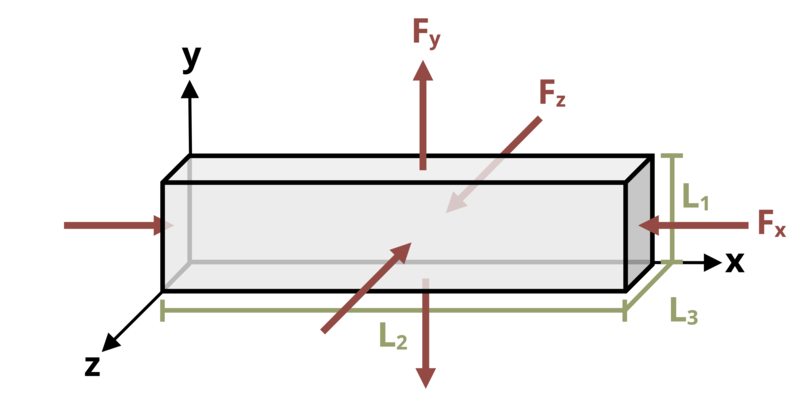
\includegraphics[keepaspectratio]{images/212.png}}
{[}Problem adapted from © Kurt Gramoll CC BY NC-SA 4.0{]}

\begin{Shaded}
\begin{Highlighting}[]
\NormalTok{\#| standalone: true}
\NormalTok{\#| viewerHeight: 600}
\NormalTok{\#| components: [viewer]}

\NormalTok{from shiny import App, render, ui, reactive}
\NormalTok{import random}
\NormalTok{import asyncio}
\NormalTok{import io}
\NormalTok{import math}
\NormalTok{import string}
\NormalTok{from datetime import datetime}
\NormalTok{from pathlib import Path}

\NormalTok{def generate\_random\_letters(length):}
\NormalTok{    \# Generate a random string of letters of specified length}
\NormalTok{    return \textquotesingle{}\textquotesingle{}.join(random.choice(string.ascii\_lowercase) for \_ in range(length))}

\NormalTok{problem\_ID="211"}
\NormalTok{Fx=reactive.Value("\_\_")}
\NormalTok{Fy=reactive.Value("\_\_")}
\NormalTok{E=reactive.Value("\_\_")}
\NormalTok{v=reactive.Value("\_\_")}
  
\NormalTok{attempts=["Timestamp,Attempt,Answer,Feedback\textbackslash{}n"]}

\NormalTok{app\_ui = ui.page\_fluid(}
\NormalTok{    \#ui.markdown("**Please enter your ID number from your instructor and click to generate your problem**"),}
\NormalTok{    \#ui.input\_text("ID","", placeholder="Enter ID Number Here"),}
\NormalTok{    \#ui.input\_action\_button("generate\_problem", "Generate Problem", class\_="btn{-}primary"),}
\NormalTok{    ui.markdown("**Problem Statement**"),}
\NormalTok{    ui.output\_ui("ui\_problem\_statement"),}
\NormalTok{    ui.input\_text("answer","Your Answer in units of in\textbackslash{}u00B3", placeholder="Please enter your answer"),}
\NormalTok{    ui.input\_action\_button("submit", "Check Answer", class\_="btn{-}primary"),}
\NormalTok{    \#ui.download\_button("download", "Download File to Submit", class\_="btn{-}success"),}
\NormalTok{)}

\NormalTok{def server(input, output, session):}
\NormalTok{    \# Initialize a counter for attempts}
\NormalTok{    attempt\_counter = reactive.Value(0)}

\NormalTok{    @output}
\NormalTok{    @render.ui}
\NormalTok{    def ui\_problem\_statement():}
\NormalTok{        randomize\_vars()}
\NormalTok{        return[ui.markdown(f"A rectangular block is pulled in two directions. Determine the total change in volume. Assume force F\textless{}sub\textgreater{}x\textless{}/sub\textgreater{} = \{Fx()\} kips, force F\textless{}sub\textgreater{}y\textless{}/sub\textgreater{} = \{Fy()\} kips, E = \{E()\} x 10\textless{}sup\textgreater{}6\textless{}/sup\textgreater{} psi, and ν = \{v()\}. Let L\textless{}sub\textgreater{}1\textless{}/sub\textgreater{} = 3 cm, L\textless{}sub\textgreater{}2\textless{}/sub\textgreater{} = 10 cm, and the width of the block be 1 cm.")]}
    
\NormalTok{    \#@reactive.Effect}
\NormalTok{    \#@reactive.event(input.generate\_problem)}
\NormalTok{    def randomize\_vars():}
\NormalTok{        random.seed(101)}
\NormalTok{        Fx.set(random.randrange(50,200,1)/10)}
\NormalTok{        Fy.set(random.randrange(50,200,1)/10)}
\NormalTok{        E.set(random.randrange(75,150,1)/10)}
\NormalTok{        v.set(random.randrange(20,40,1)/100)}
        
\NormalTok{    @reactive.Effect}
\NormalTok{    @reactive.event(input.submit)}
\NormalTok{    def \_():}
\NormalTok{        attempt\_counter.set(attempt\_counter() + 1)  \# Increment the attempt counter on each submission.}
\NormalTok{        sigmax = Fx()/4}
\NormalTok{        sigmay=Fy()/5}
\NormalTok{        strainx = (sigmax{-}v()*sigmay)/(E()*1000)}
\NormalTok{        strainy = (sigmay{-}v()*sigmax)/(E()*1000)}
\NormalTok{        strainz = ({-}v()*(sigmax+sigmay))/(E()*1000)}
\NormalTok{        LxN = 10+10*strainx}
\NormalTok{        LyN = 8+8*strainy}
\NormalTok{        LzN = 0.5+0.5*strainz}
\NormalTok{        VN = LxN*LyN*LzN}
\NormalTok{        Vo = 10*8*0.5}
\NormalTok{        instr= VN{-}Vo}
\NormalTok{        if math.isclose(float(input.answer()), instr, rel\_tol=0.01):}
\NormalTok{            check = "*Correct*"}
\NormalTok{            correct\_indicator = "JL"}
\NormalTok{        else:}
\NormalTok{            check = "*Not Correct.*"}
\NormalTok{            correct\_indicator = "JG"}

\NormalTok{        \# Generate random parts for the encoded attempt.}
\NormalTok{        random\_start = generate\_random\_letters(4)}
\NormalTok{        random\_middle = generate\_random\_letters(4)}
\NormalTok{        random\_end = generate\_random\_letters(4)}
\NormalTok{        \#encoded\_attempt = f"\{random\_start\}\{problem\_ID\}{-}\{random\_middle\}\{attempt\_counter()\}\{correct\_indicator\}{-}\{random\_end\}\{input.ID()\}"}

\NormalTok{        \# Store the most recent encoded attempt in a reactive value so it persists across submissions}
\NormalTok{        \#session.encoded\_attempt = reactive.Value(encoded\_attempt)}

\NormalTok{        \# Append the attempt data to the attempts list without the encoded attempt}
\NormalTok{        attempts.append(f"\{datetime.now()\}, \{attempt\_counter()\}, \{input.answer()\}, \{check\}\textbackslash{}n")}

\NormalTok{        \# Show feedback to the user.}
\NormalTok{        feedback = ui.markdown(f"Your answer of \{input.answer()\} is \{check\}.")}
\NormalTok{        m = ui.modal(}
\NormalTok{            feedback,}
\NormalTok{            title="Feedback",}
\NormalTok{            easy\_close=True}
\NormalTok{        )}
\NormalTok{        ui.modal\_show(m)}

\NormalTok{    \#@render.download(filename=lambda: f"Problem\_Log{-}\{problem\_ID\}{-}\{input.ID()\}.csv")}
\NormalTok{    async def download():}
\NormalTok{        \# Start the CSV with the encoded attempt (without label)}
\NormalTok{        final\_encoded = session.encoded\_attempt() if session.encoded\_attempt is not None else "No attempts"}
\NormalTok{        yield f"\{final\_encoded\}\textbackslash{}n\textbackslash{}n"}
        
\NormalTok{        \# Write the header for the remaining CSV data once}
\NormalTok{        yield "Timestamp,Attempt,Answer,Feedback\textbackslash{}n"}
        
\NormalTok{        \# Write the attempts data, ensure that the header from the attempts list is not written again}
\NormalTok{        for attempt in attempts[1:]:  \# Skip the first element which is the header}
\NormalTok{            await asyncio.sleep(0.25)  \# This delay may not be necessary; adjust as needed}
\NormalTok{            yield attempt}

\NormalTok{\# App installation}
\NormalTok{app = App(app\_ui, server)}
\end{Highlighting}
\end{Shaded}

\chapter*{Problem 4.30 - Multiaxial Hooke's
Law}\label{problem-4.30---multiaxial-hookes-law}
\addcontentsline{toc}{chapter}{Problem 4.30 - Multiaxial Hooke's Law}

\markboth{Problem 4.30 - Multiaxial Hooke's Law}{Problem 4.30 -
Multiaxial Hooke's Law}

\pandocbounded{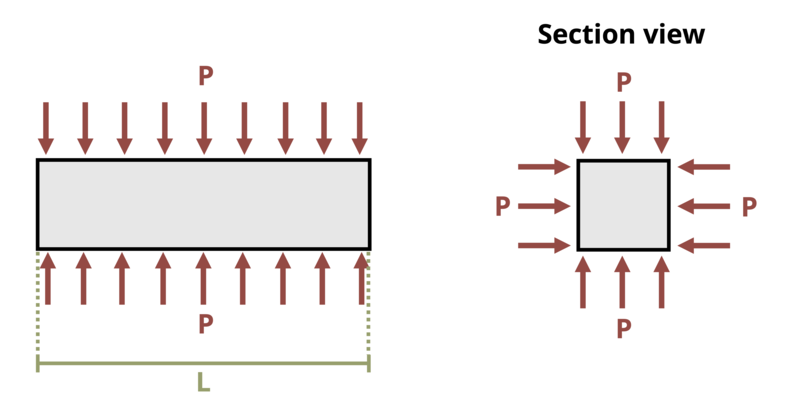
\includegraphics[keepaspectratio]{images/215.png}}
{[}Problem adapted from © Kurt Gramoll CC BY NC-SA 4.0{]}

\begin{Shaded}
\begin{Highlighting}[]
\NormalTok{\#| standalone: true}
\NormalTok{\#| viewerHeight: 600}
\NormalTok{\#| components: [viewer]}

\NormalTok{from shiny import App, render, ui, reactive}
\NormalTok{import random}
\NormalTok{import asyncio}
\NormalTok{import io}
\NormalTok{import math}
\NormalTok{import string}
\NormalTok{from datetime import datetime}
\NormalTok{from pathlib import Path}

\NormalTok{def generate\_random\_letters(length):}
\NormalTok{    \# Generate a random string of letters of specified length}
\NormalTok{    return \textquotesingle{}\textquotesingle{}.join(random.choice(string.ascii\_lowercase) for \_ in range(length))}

\NormalTok{problem\_ID="215"}
\NormalTok{L=reactive.Value("\_\_")}
\NormalTok{P=reactive.Value("\_\_")}
\NormalTok{E=reactive.Value("\_\_")}
\NormalTok{v=reactive.Value("\_\_")}
  
\NormalTok{attempts=["Timestamp,Attempt,Answer,Feedback\textbackslash{}n"]}

\NormalTok{app\_ui = ui.page\_fluid(}
\NormalTok{    \#ui.markdown("**Please enter your ID number from your instructor and click to generate your problem**"),}
\NormalTok{    \#ui.input\_text("ID","", placeholder="Enter ID Number Here"),}
\NormalTok{    \#ui.input\_action\_button("generate\_problem", "Generate Problem", class\_="btn{-}primary"),}
\NormalTok{    ui.markdown("**Problem Statement**"),}
\NormalTok{    ui.output\_ui("ui\_problem\_statement"),}
\NormalTok{    ui.input\_text("answer","Your Answer in units of mm", placeholder="Please enter your answer"),}
\NormalTok{    ui.input\_action\_button("submit", "Check Answer", class\_="btn{-}primary"),}
\NormalTok{    \#ui.download\_button("download", "Download File to Submit", class\_="btn{-}success"),}
\NormalTok{)}

\NormalTok{def server(input, output, session):}
\NormalTok{    \# Initialize a counter for attempts}
\NormalTok{    attempt\_counter = reactive.Value(0)}

\NormalTok{    @output}
\NormalTok{    @render.ui}
\NormalTok{    def ui\_problem\_statement():}
\NormalTok{        randomize\_vars()}
\NormalTok{        return[ui.markdown(f"A bar of length L = \{L()\} mm is subjected to a pressure P = \{P()\} kPa on the two long dimensions (not the ends) as shown. Assuming E = \{E()\} kPa and ν = \{v()\}, determine the change in length of the L = \{L()\} mm side.")]}
    
\NormalTok{    \#@reactive.Effect}
\NormalTok{    \#@reactive.event(input.generate\_problem)}
\NormalTok{    def randomize\_vars():}
\NormalTok{        random.seed(101)}
\NormalTok{        L.set(random.randrange(250,750,10))}
\NormalTok{        P.set(random.randrange(1,10,1)/10)}
\NormalTok{        E.set(random.randrange(400,900))}
\NormalTok{        v.set(random.randrange(30,45,1)/100)}
        
\NormalTok{    @reactive.Effect}
\NormalTok{    @reactive.event(input.submit)}
\NormalTok{    def \_():}
\NormalTok{        attempt\_counter.set(attempt\_counter() + 1)  \# Increment the attempt counter on each submission.}
\NormalTok{        strainz = (v()*2*P())/E()}
\NormalTok{        instr= L()*strainz}
\NormalTok{        if math.isclose(float(input.answer()), instr, rel\_tol=0.01):}
\NormalTok{            check = "*Correct*"}
\NormalTok{            correct\_indicator = "JL"}
\NormalTok{        else:}
\NormalTok{            check = "*Not Correct.*"}
\NormalTok{            correct\_indicator = "JG"}

\NormalTok{        \# Generate random parts for the encoded attempt.}
\NormalTok{        random\_start = generate\_random\_letters(4)}
\NormalTok{        random\_middle = generate\_random\_letters(4)}
\NormalTok{        random\_end = generate\_random\_letters(4)}
\NormalTok{        \#encoded\_attempt = f"\{random\_start\}\{problem\_ID\}{-}\{random\_middle\}\{attempt\_counter()\}\{correct\_indicator\}{-}\{random\_end\}\{input.ID()\}"}

\NormalTok{        \# Store the most recent encoded attempt in a reactive value so it persists across submissions}
\NormalTok{        \#session.encoded\_attempt = reactive.Value(encoded\_attempt)}

\NormalTok{        \# Append the attempt data to the attempts list without the encoded attempt}
\NormalTok{        attempts.append(f"\{datetime.now()\}, \{attempt\_counter()\}, \{input.answer()\}, \{check\}\textbackslash{}n")}

\NormalTok{        \# Show feedback to the user.}
\NormalTok{        feedback = ui.markdown(f"Your answer of \{input.answer()\} is \{check\}.")}
\NormalTok{        m = ui.modal(}
\NormalTok{            feedback,}
\NormalTok{            title="Feedback",}
\NormalTok{            easy\_close=True}
\NormalTok{        )}
\NormalTok{        ui.modal\_show(m)}

\NormalTok{    \#@render.download(filename=lambda: f"Problem\_Log{-}\{problem\_ID\}{-}\{input.ID()\}.csv")}
\NormalTok{    async def download():}
\NormalTok{        \# Start the CSV with the encoded attempt (without label)}
\NormalTok{        final\_encoded = session.encoded\_attempt() if session.encoded\_attempt is not None else "No attempts"}
\NormalTok{        yield f"\{final\_encoded\}\textbackslash{}n\textbackslash{}n"}
        
\NormalTok{        \# Write the header for the remaining CSV data once}
\NormalTok{        yield "Timestamp,Attempt,Answer,Feedback\textbackslash{}n"}
        
\NormalTok{        \# Write the attempts data, ensure that the header from the attempts list is not written again}
\NormalTok{        for attempt in attempts[1:]:  \# Skip the first element which is the header}
\NormalTok{            await asyncio.sleep(0.25)  \# This delay may not be necessary; adjust as needed}
\NormalTok{            yield attempt}

\NormalTok{\# App installation}
\NormalTok{app = App(app\_ui, server)}
\end{Highlighting}
\end{Shaded}

\chapter*{Problem 4.31 - Multiaxial Hooke's
Law}\label{problem-4.31---multiaxial-hookes-law}
\addcontentsline{toc}{chapter}{Problem 4.31 - Multiaxial Hooke's Law}

\markboth{Problem 4.31 - Multiaxial Hooke's Law}{Problem 4.31 -
Multiaxial Hooke's Law}

\pandocbounded{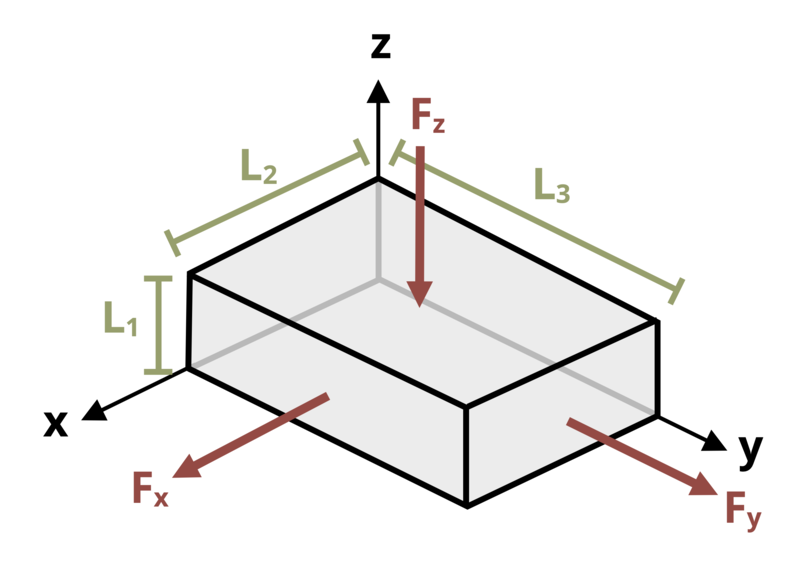
\includegraphics[keepaspectratio]{images/217.png}}
{[}Problem adapted from © Kurt Gramoll CC BY NC-SA 4.0{]}

\begin{Shaded}
\begin{Highlighting}[]
\NormalTok{\#| standalone: true}
\NormalTok{\#| viewerHeight: 600}
\NormalTok{\#| components: [viewer]}

\NormalTok{from shiny import App, render, ui, reactive}
\NormalTok{import random}
\NormalTok{import asyncio}
\NormalTok{import io}
\NormalTok{import math}
\NormalTok{import string}
\NormalTok{from datetime import datetime}
\NormalTok{from pathlib import Path}

\NormalTok{def generate\_random\_letters(length):}
\NormalTok{    \# Generate a random string of letters of specified length}
\NormalTok{    return \textquotesingle{}\textquotesingle{}.join(random.choice(string.ascii\_lowercase) for \_ in range(length))}

\NormalTok{problem\_ID="217"}
\NormalTok{Fx=reactive.Value("\_\_")}
\NormalTok{Fy=reactive.Value("\_\_")}
\NormalTok{Fz=reactive.Value("\_\_")}
  
\NormalTok{attempts=["Timestamp,Attempt,Answer,Feedback\textbackslash{}n"]}

\NormalTok{app\_ui = ui.page\_fluid(}
\NormalTok{    \#ui.markdown("**Please enter your ID number from your instructor and click to generate your problem**"),}
\NormalTok{    \#ui.input\_text("ID","", placeholder="Enter ID Number Here"),}
\NormalTok{    \#ui.input\_action\_button("generate\_problem", "Generate Problem", class\_="btn{-}primary"),}
\NormalTok{    ui.markdown("**Problem Statement**"),}
\NormalTok{    ui.output\_ui("ui\_problem\_statement"),}
\NormalTok{    ui.input\_text("answer","Your Answer in units of in", placeholder="Please enter your answer"),}
\NormalTok{    ui.input\_action\_button("submit", "Check Answer", class\_="btn{-}primary"),}
\NormalTok{    \#ui.download\_button("download", "Download File to Submit", class\_="btn{-}success"),}
\NormalTok{)}

\NormalTok{def server(input, output, session):}
\NormalTok{    \# Initialize a counter for attempts}
\NormalTok{    attempt\_counter = reactive.Value(0)}

\NormalTok{    @output}
\NormalTok{    @render.ui}
\NormalTok{    def ui\_problem\_statement():}
\NormalTok{        randomize\_vars()}
\NormalTok{        return[ui.markdown(f"A small brass sample is subjected to loads on each of its three surfaces, where F\textless{}sub\textgreater{}x\textless{}/sub\textgreater{} = \{Fx()\} kips, F\textless{}sub\textgreater{}y\textless{}/sub\textgreater{} = \{Fy()\} kips, and F\textless{}sub\textgreater{}z\textless{}/sub\textgreater{} = \{Fz()\} kips. Assuming E = 15 x 10\textless{}sup\textgreater{}6\textless{}/sup\textgreater{} psi and ν = 0.34, determine the total change in length in the z{-}direction. Let L\textless{}sub\textgreater{}1\textless{}/sub\textgreater{} = 1 in, L\textless{}sub\textgreater{}2\textless{}/sub\textgreater{} = 2 in, and L\textless{}sub\textgreater{}3\textless{}/sub\textgreater{} = 3 in. Note a minus sign if the length decreases.")]}
    
\NormalTok{    \#@reactive.Effect}
\NormalTok{    \#@reactive.event(input.generate\_problem)}
\NormalTok{    def randomize\_vars():}
\NormalTok{        random.seed(101)}
\NormalTok{        Fx.set(random.randrange(50,200,1)/10)}
\NormalTok{        Fy.set(random.randrange(50,200,1)/10)}
\NormalTok{        Fz.set(random.randrange(50,200,1)/10)}
        
\NormalTok{    @reactive.Effect}
\NormalTok{    @reactive.event(input.submit)}
\NormalTok{    def \_():}
\NormalTok{        attempt\_counter.set(attempt\_counter() + 1)  \# Increment the attempt counter on each submission.}
\NormalTok{        sigmax = Fx()/3}
\NormalTok{        sigmay = Fy()/2}
\NormalTok{        sigmaz = Fz()/6}
\NormalTok{        instr = ({-}sigmaz{-}0.34*(sigmax+sigmay))/(15*10**3)}
\NormalTok{        if math.isclose(float(input.answer()), instr, rel\_tol=0.01):}
\NormalTok{            check = "*Correct*"}
\NormalTok{            correct\_indicator = "JL"}
\NormalTok{        else:}
\NormalTok{            check = "*Not Correct.*"}
\NormalTok{            correct\_indicator = "JG"}

\NormalTok{        \# Generate random parts for the encoded attempt.}
\NormalTok{        random\_start = generate\_random\_letters(4)}
\NormalTok{        random\_middle = generate\_random\_letters(4)}
\NormalTok{        random\_end = generate\_random\_letters(4)}
\NormalTok{        \#encoded\_attempt = f"\{random\_start\}\{problem\_ID\}{-}\{random\_middle\}\{attempt\_counter()\}\{correct\_indicator\}{-}\{random\_end\}\{input.ID()\}"}

\NormalTok{        \# Store the most recent encoded attempt in a reactive value so it persists across submissions}
\NormalTok{        \#session.encoded\_attempt = reactive.Value(encoded\_attempt)}

\NormalTok{        \# Append the attempt data to the attempts list without the encoded attempt}
\NormalTok{        attempts.append(f"\{datetime.now()\}, \{attempt\_counter()\}, \{input.answer()\}, \{check\}\textbackslash{}n")}

\NormalTok{        \# Show feedback to the user.}
\NormalTok{        feedback = ui.markdown(f"Your answer of \{input.answer()\} is \{check\}.")}
\NormalTok{        m = ui.modal(}
\NormalTok{            feedback,}
\NormalTok{            title="Feedback",}
\NormalTok{            easy\_close=True}
\NormalTok{        )}
\NormalTok{        ui.modal\_show(m)}

\NormalTok{    \#@render.download(filename=lambda: f"Problem\_Log{-}\{problem\_ID\}{-}\{input.ID()\}.csv")}
\NormalTok{    async def download():}
\NormalTok{        \# Start the CSV with the encoded attempt (without label)}
\NormalTok{        final\_encoded = session.encoded\_attempt() if session.encoded\_attempt is not None else "No attempts"}
\NormalTok{        yield f"\{final\_encoded\}\textbackslash{}n\textbackslash{}n"}
        
\NormalTok{        \# Write the header for the remaining CSV data once}
\NormalTok{        yield "Timestamp,Attempt,Answer,Feedback\textbackslash{}n"}
        
\NormalTok{        \# Write the attempts data, ensure that the header from the attempts list is not written again}
\NormalTok{        for attempt in attempts[1:]:  \# Skip the first element which is the header}
\NormalTok{            await asyncio.sleep(0.25)  \# This delay may not be necessary; adjust as needed}
\NormalTok{            yield attempt}

\NormalTok{\# App installation}
\NormalTok{app = App(app\_ui, server)}
\end{Highlighting}
\end{Shaded}

\chapter*{Problem 4.35 - Allowable Stress/Safety
Factor}\label{problem-4.35---allowable-stresssafety-factor}
\addcontentsline{toc}{chapter}{Problem 4.35 - Allowable Stress/Safety
Factor}

\markboth{Problem 4.35 - Allowable Stress/Safety Factor}{Problem 4.35 -
Allowable Stress/Safety Factor}

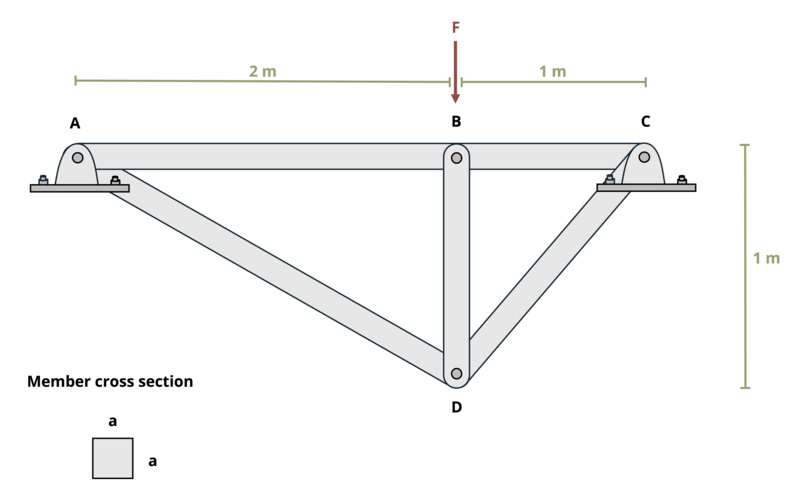
\includegraphics[width=25.16667in,height=\textheight,keepaspectratio]{images/157.png}
{[}Problem adapted from © Kurt Gramoll CC BY NC-SA 4.0{]}

\begin{Shaded}
\begin{Highlighting}[]
\NormalTok{\#| standalone: true}
\NormalTok{\#| viewerHeight: 600}
\NormalTok{\#| components: [viewer]}

\NormalTok{from shiny import App, render, ui, reactive}
\NormalTok{import random}
\NormalTok{import asyncio}
\NormalTok{import io}
\NormalTok{import math}
\NormalTok{import string}
\NormalTok{from datetime import datetime}
\NormalTok{from pathlib import Path}

\NormalTok{def generate\_random\_letters(length):}
\NormalTok{    \# Generate a random string of letters of specified length}
\NormalTok{    return \textquotesingle{}\textquotesingle{}.join(random.choice(string.ascii\_lowercase) for \_ in range(length))  }

\NormalTok{problem\_ID="157"}
\NormalTok{F=reactive.Value("\_\_")}
\NormalTok{FS=reactive.Value("\_\_")}
\NormalTok{σfail=reactive.Value("\_\_")}

\NormalTok{attempts=["Timestamp,Attempt,Answer,Feedback\textbackslash{}n"]}

\NormalTok{app\_ui = ui.page\_fluid(}
\NormalTok{    \#ui.markdown("**Please enter your ID number from your instructor and click to generate your problem**"),}
\NormalTok{    \#ui.input\_text("ID","", placeholder="Enter ID Number Here"),}
\NormalTok{    \#ui.input\_action\_button("generate\_problem", "Generate Problem", class\_="btn{-}primary"),}
\NormalTok{    ui.markdown("**Problem Statement**"),}
\NormalTok{    ui.output\_ui("ui\_problem\_statement"),}
\NormalTok{    ui.input\_text("answer","Your Answer in units of centimeters", placeholder="Please enter your answer"),}
\NormalTok{    ui.input\_action\_button("submit", "Check Answer", class\_="btn{-}primary"),}
\NormalTok{    \#ui.download\_button("download", "Download File to Submit", class\_="btn{-}success"),}
\NormalTok{)}


\NormalTok{def server(input, output, session):}
\NormalTok{    \# Initialize a counter for attempts}
\NormalTok{    attempt\_counter = reactive.Value(0)}

\NormalTok{    @output}
\NormalTok{    @render.ui}
\NormalTok{    def ui\_problem\_statement():}
\NormalTok{        randomize\_vars()}
\NormalTok{        return[ui.markdown(f"A small truss is constructed with solid square wood members and subjected to a load of F = \{F()\} kN. Determine the minimum dimension, a, of the member so that the truss will have a factor of safety of \{FS()\}. All members have the same cross{-}section. The wood has a failure stress of σ\textless{}sub\textgreater{}fail\textless{}/sub\textgreater{} = \{σfail()\} MPa.")]}
    
\NormalTok{    \#@reactive.Effect}
\NormalTok{    \#@reactive.event(input.generate\_problem)}
\NormalTok{    def randomize\_vars():}
\NormalTok{        random.seed(101)}
\NormalTok{        F.set(random.randrange(15, 50, 1))}
\NormalTok{        FS.set(random.randrange(15, 40, 1)/10)}
\NormalTok{        σfail.set(random.randrange(40, 60, 1))}
        

\NormalTok{    @reactive.Effect}
\NormalTok{    @reactive.event(input.submit)}
\NormalTok{    def \_():}
\NormalTok{        attempt\_counter.set(attempt\_counter() + 1)  \# Increment the attempt counter on each submission.}
    
\NormalTok{        dl = FS()*F()}
\NormalTok{        A = (dl/(σfail()*10**3))*100*100}
\NormalTok{        instr= math.sqrt(A)}
\NormalTok{        if math.isclose(float(input.answer()), instr, rel\_tol=0.01):}
\NormalTok{            check = "*Correct*"}
\NormalTok{            correct\_indicator = "JL"}
\NormalTok{        else:}
\NormalTok{            check = "*Not Correct.*"}
\NormalTok{            correct\_indicator = "JG"}

\NormalTok{        \# Generate random parts for the encoded attempt.}
\NormalTok{        random\_start = generate\_random\_letters(4)}
\NormalTok{        random\_middle = generate\_random\_letters(4)}
\NormalTok{        random\_end = generate\_random\_letters(4)}
\NormalTok{        \#encoded\_attempt = f"\{random\_start\}\{problem\_ID\}{-}\{random\_middle\}\{attempt\_counter()\}\{correct\_indicator\}{-}\{random\_end\}\{input.ID()\}"}

\NormalTok{        \# Store the most recent encoded attempt in a reactive value so it persists across submissions}
\NormalTok{        \#session.encoded\_attempt = reactive.Value(encoded\_attempt)}

\NormalTok{        \# Append the attempt data to the attempts list without the encoded attempt}
\NormalTok{        attempts.append(f"\{datetime.now()\}, \{attempt\_counter()\}, \{input.answer()\}, \{check\}\textbackslash{}n")}

\NormalTok{        \# Show feedback to the user.}
\NormalTok{        feedback = ui.markdown(f"Your answer of \{input.answer()\} is \{check\}.")}
\NormalTok{        m = ui.modal(}
\NormalTok{            feedback,}
\NormalTok{            title="Feedback",}
\NormalTok{            easy\_close=True}
\NormalTok{        )}
\NormalTok{        ui.modal\_show(m)}

\NormalTok{    \#@render.download(filename=lambda: f"Problem\_Log{-}\{problem\_ID\}{-}\{input.ID()\}.csv")}
\NormalTok{    async def download():}
\NormalTok{        \# Start the CSV with the encoded attempt (without label)}
\NormalTok{        final\_encoded = session.encoded\_attempt() if session.encoded\_attempt is not None else "No attempts"}
\NormalTok{        yield f"\{final\_encoded\}\textbackslash{}n\textbackslash{}n"}
        
\NormalTok{        \# Write the header for the remaining CSV data once}
\NormalTok{        yield "Timestamp,Attempt,Answer,Feedback\textbackslash{}n"}
        
\NormalTok{        \# Write the attempts data, ensure that the header from the attempts list is not written again}
\NormalTok{        for attempt in attempts[1:]:  \# Skip the first element which is the header}
\NormalTok{            await asyncio.sleep(0.25)  \# This delay may not be necessary; adjust as needed}
\NormalTok{            yield attempt}


\NormalTok{\# App installation}
\NormalTok{app = App(app\_ui, server)}
\end{Highlighting}
\end{Shaded}

\part{Chapter 5 Problems}

\chapter*{Problem 5.1 - Axial Stress}\label{problem-5.1---axial-stress}
\addcontentsline{toc}{chapter}{Problem 5.1 - Axial Stress}

\markboth{Problem 5.1 - Axial Stress}{Problem 5.1 - Axial Stress}

{[}Problem adapted from © Chris Galitz CC BY NC-SA 4.0{]}

\begin{Shaded}
\begin{Highlighting}[]
\NormalTok{\#| standalone: true}
\NormalTok{\#| viewerHeight: 600}
\NormalTok{\#| components: [viewer]}

\NormalTok{from shiny import App, render, ui, reactive}
\NormalTok{import random}
\NormalTok{import asyncio}
\NormalTok{import io}
\NormalTok{import math}
\NormalTok{import string}
\NormalTok{from datetime import datetime}
\NormalTok{from pathlib import Path}

\NormalTok{def generate\_random\_letters(length):}
\NormalTok{    \# Generate a random string of letters of specified length}
\NormalTok{    return \textquotesingle{}\textquotesingle{}.join(random.choice(string.ascii\_lowercase) for \_ in range(length))  }

\NormalTok{problem\_ID="662"}
\NormalTok{L=reactive.Value("\_\_")}
\NormalTok{P=reactive.Value("\_\_")}

\NormalTok{attempts=["Timestamp,Attempt,Answer,Feedback\textbackslash{}n"]}

\NormalTok{app\_ui = ui.page\_fluid(}
\NormalTok{    \#ui.markdown("**Please enter your ID number from your instructor and click to generate your problem**"),}
\NormalTok{    \#ui.input\_text("ID","", placeholder="Enter ID Number Here"),}
\NormalTok{    \#ui.input\_action\_button("generate\_problem", "Generate Problem", class\_="btn{-}primary"),}
\NormalTok{    ui.markdown("**Problem Statement**"),}
\NormalTok{    ui.output\_ui("ui\_problem\_statement"),}
\NormalTok{    ui.input\_text("answer","Your Answer in units of ksi", placeholder="Please enter your answer"),}
\NormalTok{    ui.input\_action\_button("submit", "Check Answer", class\_="btn{-}primary"),}
\NormalTok{    \#ui.download\_button("download", "Download File to Submit", class\_="btn{-}success"),}
\NormalTok{)}

\NormalTok{def server(input, output, session):}
\NormalTok{    \# Initialize a counter for attempts}
\NormalTok{    attempt\_counter = reactive.Value(0)}

\NormalTok{    @output}
\NormalTok{    @render.ui}
\NormalTok{    def ui\_problem\_statement():}
\NormalTok{        randomize\_vars()}
\NormalTok{        return[ui.markdown(f"A W18 x 50 structural steel column of length L = \{L()\} ft is subjected to a compressive axial load P = \{P()\} kips. Determine the magnitude of the average normal stress at the base of the column, including self{-}weight.")]}
    
\NormalTok{    \#@reactive.Effect}
\NormalTok{    \#@reactive.event(input.generate\_problem)}
\NormalTok{    def randomize\_vars():}
\NormalTok{        random.seed(101)}
\NormalTok{        L.set(random.randrange(10,25,1))}
\NormalTok{        P.set(random.randrange(10,100,1))}
        
\NormalTok{    @reactive.Effect}
\NormalTok{    @reactive.event(input.submit)}
\NormalTok{    def \_():}
\NormalTok{        attempt\_counter.set(attempt\_counter() + 1)  \# Increment the attempt counter on each submission.}
\NormalTok{        Weight=(50*L())/1000}
\NormalTok{        LoadTot=P()+Weight}
\NormalTok{        instr=LoadTot/14.7}
\NormalTok{        if math.isclose(float(input.answer()), instr, rel\_tol=0.01):}
\NormalTok{            check = "*Correct*"}
\NormalTok{            correct\_indicator = "JL"}
\NormalTok{        else:}
\NormalTok{            check = "*Not Correct.*"}
\NormalTok{            correct\_indicator = "JG"}

\NormalTok{        \# Generate random parts for the encoded attempt.}
\NormalTok{        random\_start = generate\_random\_letters(4)}
\NormalTok{        random\_middle = generate\_random\_letters(4)}
\NormalTok{        random\_end = generate\_random\_letters(4)}
\NormalTok{        \#encoded\_attempt = f"\{random\_start\}\{problem\_ID\}{-}\{random\_middle\}\{attempt\_counter()\}\{correct\_indicator\}{-}\{random\_end\}\{input.ID()\}"}

\NormalTok{        \# Store the most recent encoded attempt in a reactive value so it persists across submissions}
\NormalTok{        \#session.encoded\_attempt = reactive.Value(encoded\_attempt)}

\NormalTok{        \# Append the attempt data to the attempts list without the encoded attempt}
\NormalTok{        attempts.append(f"\{datetime.now()\}, \{attempt\_counter()\}, \{input.answer()\}, \{check\}\textbackslash{}n")}

\NormalTok{        \# Show feedback to the user.}
\NormalTok{        feedback = ui.markdown(f"Your answer of \{input.answer()\} is \{check\}.")}
\NormalTok{        m = ui.modal(}
\NormalTok{            feedback,}
\NormalTok{            title="Feedback",}
\NormalTok{            easy\_close=True}
\NormalTok{        )}
\NormalTok{        ui.modal\_show(m)}

\NormalTok{    \#@render.download(filename=lambda: f"Problem\_Log{-}\{problem\_ID\}{-}\{input.ID()\}.csv")}
\NormalTok{    async def download():}
\NormalTok{        \# Start the CSV with the encoded attempt (without label)}
\NormalTok{        final\_encoded = session.encoded\_attempt() if session.encoded\_attempt is not None else "No attempts"}
\NormalTok{        yield f"\{final\_encoded\}\textbackslash{}n\textbackslash{}n"}
        
\NormalTok{        \# Write the header for the remaining CSV data once}
\NormalTok{        yield "Timestamp,Attempt,Answer,Feedback\textbackslash{}n"}
        
\NormalTok{        \# Write the attempts data, ensure that the header from the attempts list is not written again}
\NormalTok{        for attempt in attempts[1:]:  \# Skip the first element which is the header}
\NormalTok{            await asyncio.sleep(0.25)  \# This delay may not be necessary; adjust as needed}
\NormalTok{            yield attempt}

\NormalTok{\# App installation}
\NormalTok{app = App(app\_ui, server)}
\end{Highlighting}
\end{Shaded}

\chapter*{Problem 5.2 - Axial Stress}\label{problem-5.2---axial-stress}
\addcontentsline{toc}{chapter}{Problem 5.2 - Axial Stress}

\markboth{Problem 5.2 - Axial Stress}{Problem 5.2 - Axial Stress}

\pandocbounded{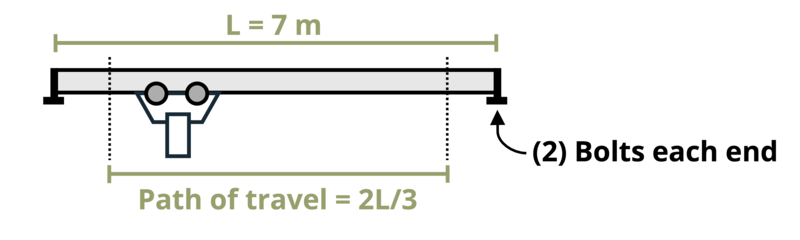
\includegraphics[keepaspectratio]{images/663.png}}
{[}Problem adapted from © Chris Galitz CC BY NC-SA 4.0{]}

\begin{Shaded}
\begin{Highlighting}[]
\NormalTok{\#| standalone: true}
\NormalTok{\#| viewerHeight: 600}
\NormalTok{\#| components: [viewer]}

\NormalTok{from shiny import App, render, ui, reactive}
\NormalTok{import random}
\NormalTok{import asyncio}
\NormalTok{import io}
\NormalTok{import math}
\NormalTok{import string}
\NormalTok{from datetime import datetime}
\NormalTok{from pathlib import Path}

\NormalTok{def generate\_random\_letters(length):}
\NormalTok{    \# Generate a random string of letters of specified length}
\NormalTok{    return \textquotesingle{}\textquotesingle{}.join(random.choice(string.ascii\_lowercase) for \_ in range(length))  }

\NormalTok{problem\_ID="663"}
\NormalTok{cap=reactive.Value("\_\_")}
\NormalTok{L=reactive.Value("\_\_")}
\NormalTok{sigmay=reactive.Value("\_\_")}
\NormalTok{FS=reactive.Value("\_\_")}

\NormalTok{attempts=["Timestamp,Attempt,Answer,Feedback\textbackslash{}n"]}

\NormalTok{app\_ui = ui.page\_fluid(}
\NormalTok{    \#ui.markdown("**Please enter your ID number from your instructor and click to generate your problem**"),}
\NormalTok{    \#ui.input\_text("ID","", placeholder="Enter ID Number Here"),}
\NormalTok{    \#ui.input\_action\_button("generate\_problem", "Generate Problem", class\_="btn{-}primary"),}
\NormalTok{    ui.markdown("**Problem Statement**"),}
\NormalTok{    ui.output\_ui("ui\_problem\_statement"),}
\NormalTok{    ui.input\_text("answer","Your Answer in units of mm", placeholder="Please enter your answer"),}
\NormalTok{    ui.input\_action\_button("submit", "Check Answer", class\_="btn{-}primary"),}
\NormalTok{    \#ui.download\_button("download", "Download File to Submit", class\_="btn{-}success"),}
\NormalTok{)}

\NormalTok{def server(input, output, session):}
\NormalTok{    \# Initialize a counter for attempts}
\NormalTok{    attempt\_counter = reactive.Value(0)}

\NormalTok{    @output}
\NormalTok{    @render.ui}
\NormalTok{    def ui\_problem\_statement():}
\NormalTok{        randomize\_vars()}
\NormalTok{        return[ui.markdown(f"A chain hoist with a labeled capacity of \{cap()\} kN tavels along the middle 2/3 of a beam of length L = \{L()\} m that is bolted to a ceiling with two bolts at each end. Each bolt has a yield strength, σ\textless{}sub\textgreater{}y\textless{}/sub\textgreater{} = \{sigmay()\} MPa. Determine the minimum required bolt diameter using a factor of safety of \{FS()\}.")]}
    
\NormalTok{    \#@reactive.Effect}
\NormalTok{    \#@reactive.event(input.generate\_problem)}
\NormalTok{    def randomize\_vars():}
\NormalTok{        random.seed(101)}
\NormalTok{        cap.set(random.randrange(50,150,5))}
\NormalTok{        L.set(random.randrange(5,20,1))}
\NormalTok{        sigmay.set(random.randrange(400,700,10))}
\NormalTok{        FS.set(random.randrange(15,30,1)/10)}
        
\NormalTok{    @reactive.Effect}
\NormalTok{    @reactive.event(input.submit)}
\NormalTok{    def \_():}
\NormalTok{        attempt\_counter.set(attempt\_counter() + 1)  \# Increment the attempt counter on each submission.}
\NormalTok{        Fbolt=cap()*5/6/2}
\NormalTok{        Fdes=Fbolt*FS()}
\NormalTok{        Amin=Fdes/(sigmay()/1000)}
\NormalTok{        instr=math.sqrt(4*Amin/math.pi)}
\NormalTok{        if math.isclose(float(input.answer()), instr, rel\_tol=0.01):}
\NormalTok{            check = "*Correct*"}
\NormalTok{            correct\_indicator = "JL"}
\NormalTok{        else:}
\NormalTok{            check = "*Not Correct.*"}
\NormalTok{            correct\_indicator = "JG"}

\NormalTok{        \# Generate random parts for the encoded attempt.}
\NormalTok{        random\_start = generate\_random\_letters(4)}
\NormalTok{        random\_middle = generate\_random\_letters(4)}
\NormalTok{        random\_end = generate\_random\_letters(4)}
\NormalTok{        \#encoded\_attempt = f"\{random\_start\}\{problem\_ID\}{-}\{random\_middle\}\{attempt\_counter()\}\{correct\_indicator\}{-}\{random\_end\}\{input.ID()\}"}

\NormalTok{        \# Store the most recent encoded attempt in a reactive value so it persists across submissions}
\NormalTok{        \#session.encoded\_attempt = reactive.Value(encoded\_attempt)}

\NormalTok{        \# Append the attempt data to the attempts list without the encoded attempt}
\NormalTok{        attempts.append(f"\{datetime.now()\}, \{attempt\_counter()\}, \{input.answer()\}, \{check\}\textbackslash{}n")}

\NormalTok{        \# Show feedback to the user.}
\NormalTok{        feedback = ui.markdown(f"Your answer of \{input.answer()\} is \{check\}.")}
\NormalTok{        m = ui.modal(}
\NormalTok{            feedback,}
\NormalTok{            title="Feedback",}
\NormalTok{            easy\_close=True}
\NormalTok{        )}
\NormalTok{        ui.modal\_show(m)}

\NormalTok{    \#@render.download(filename=lambda: f"Problem\_Log{-}\{problem\_ID\}{-}\{input.ID()\}.csv")}
\NormalTok{    async def download():}
\NormalTok{        \# Start the CSV with the encoded attempt (without label)}
\NormalTok{        final\_encoded = session.encoded\_attempt() if session.encoded\_attempt is not None else "No attempts"}
\NormalTok{        yield f"\{final\_encoded\}\textbackslash{}n\textbackslash{}n"}
        
\NormalTok{        \# Write the header for the remaining CSV data once}
\NormalTok{        yield "Timestamp,Attempt,Answer,Feedback\textbackslash{}n"}
        
\NormalTok{        \# Write the attempts data, ensure that the header from the attempts list is not written again}
\NormalTok{        for attempt in attempts[1:]:  \# Skip the first element which is the header}
\NormalTok{            await asyncio.sleep(0.25)  \# This delay may not be necessary; adjust as needed}
\NormalTok{            yield attempt}

\NormalTok{\# App installation}
\NormalTok{app = App(app\_ui, server)}
\end{Highlighting}
\end{Shaded}

\chapter*{Problem 5.6 - Stress
Concentrations}\label{problem-5.6---stress-concentrations}
\addcontentsline{toc}{chapter}{Problem 5.6 - Stress Concentrations}

\markboth{Problem 5.6 - Stress Concentrations}{Problem 5.6 - Stress
Concentrations}

\pandocbounded{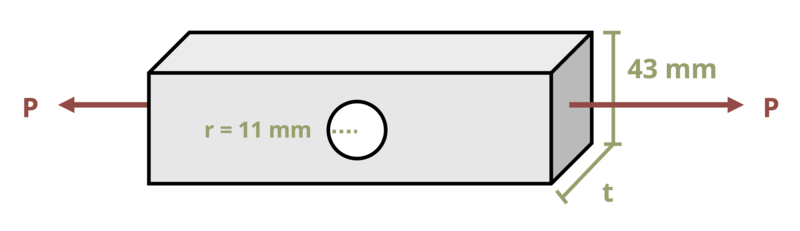
\includegraphics[keepaspectratio]{images/664.png}}
{[}Problem adapted from © Chris Galitz CC BY NC-SA 4.0{]}

\begin{Shaded}
\begin{Highlighting}[]
\NormalTok{\#| standalone: true}
\NormalTok{\#| viewerHeight: 600}
\NormalTok{\#| components: [viewer]}

\NormalTok{from shiny import App, render, ui, reactive}
\NormalTok{import random}
\NormalTok{import asyncio}
\NormalTok{import io}
\NormalTok{import math}
\NormalTok{import string}
\NormalTok{from datetime import datetime}
\NormalTok{from pathlib import Path}

\NormalTok{def generate\_random\_letters(length):}
\NormalTok{    \# Generate a random string of letters of specified length}
\NormalTok{    return \textquotesingle{}\textquotesingle{}.join(random.choice(string.ascii\_lowercase) for \_ in range(length))  }

\NormalTok{problem\_ID="664"}
\NormalTok{t=reactive.Value("\_\_")}
\NormalTok{P=reactive.Value("\_\_")}

\NormalTok{attempts=["Timestamp,Attempt,Answer,Feedback\textbackslash{}n"]}

\NormalTok{app\_ui = ui.page\_fluid(}
\NormalTok{    \#ui.markdown("**Please enter your ID number from your instructor and click to generate your problem**"),}
\NormalTok{    \#ui.input\_text("ID","", placeholder="Enter ID Number Here"),}
\NormalTok{    \#ui.input\_action\_button("generate\_problem", "Generate Problem", class\_="btn{-}primary"),}
\NormalTok{    ui.markdown("**Problem Statement**"),}
\NormalTok{    ui.output\_ui("ui\_problem\_statement"),}
\NormalTok{    ui.input\_text("answer","Your Answer in units of MPa", placeholder="Please enter your answer"),}
\NormalTok{    ui.input\_action\_button("submit", "Check Answer", class\_="btn{-}primary"),}
\NormalTok{    \#ui.download\_button("download", "Download File to Submit", class\_="btn{-}success"),}
\NormalTok{)}

\NormalTok{def server(input, output, session):}
\NormalTok{    \# Initialize a counter for attempts}
\NormalTok{    attempt\_counter = reactive.Value(0)}

\NormalTok{    @output}
\NormalTok{    @render.ui}
\NormalTok{    def ui\_problem\_statement():}
\NormalTok{        randomize\_vars()}
\NormalTok{        return[ui.markdown(f"A flat bar of thickness t = \{t()\} mm contains a hole as shown. The bar is subjected to a tensile load P = \{P()\} kN. Determine the maximum tensile stress in the bar.")]}
    
\NormalTok{    \#@reactive.Effect}
\NormalTok{    \#@reactive.event(input.generate\_problem)}
\NormalTok{    def randomize\_vars():}
\NormalTok{        random.seed(101)}
\NormalTok{        t.set(random.randrange(10, 25, 1))}
\NormalTok{        P.set(random.randrange(10, 100, 1)/10)}
        
\NormalTok{    @reactive.Effect}
\NormalTok{    @reactive.event(input.submit)}
\NormalTok{    def \_():}
\NormalTok{        attempt\_counter.set(attempt\_counter() + 1)  \# Increment the attempt counter on each submission.}
\NormalTok{        sigma\_norm = P()/(t()*(43{-}22))*1000}
\NormalTok{        instr= 2.15*(sigma\_norm)}
\NormalTok{        if math.isclose(float(input.answer()), instr, rel\_tol=0.03):}
\NormalTok{            check = "*Correct*"}
\NormalTok{            correct\_indicator = "JL"}
\NormalTok{        else:}
\NormalTok{            check = "*Not Correct.*"}
\NormalTok{            correct\_indicator = "JG"}

\NormalTok{        \# Generate random parts for the encoded attempt.}
\NormalTok{        random\_start = generate\_random\_letters(4)}
\NormalTok{        random\_middle = generate\_random\_letters(4)}
\NormalTok{        random\_end = generate\_random\_letters(4)}
\NormalTok{        \#encoded\_attempt = f"\{random\_start\}\{problem\_ID\}{-}\{random\_middle\}\{attempt\_counter()\}\{correct\_indicator\}{-}\{random\_end\}\{input.ID()\}"}

\NormalTok{        \# Store the most recent encoded attempt in a reactive value so it persists across submissions}
\NormalTok{        \#session.encoded\_attempt = reactive.Value(encoded\_attempt)}

\NormalTok{        \# Append the attempt data to the attempts list without the encoded attempt}
\NormalTok{        attempts.append(f"\{datetime.now()\}, \{attempt\_counter()\}, \{input.answer()\}, \{check\}\textbackslash{}n")}

\NormalTok{        \# Show feedback to the user.}
\NormalTok{        feedback = ui.markdown(f"Your answer of \{input.answer()\} is \{check\}.")}
\NormalTok{        m = ui.modal(}
\NormalTok{            feedback,}
\NormalTok{            title="Feedback",}
\NormalTok{            easy\_close=True}
\NormalTok{        )}
\NormalTok{        ui.modal\_show(m)}

\NormalTok{    \#@render.download(filename=lambda: f"Problem\_Log{-}\{problem\_ID\}{-}\{input.ID()\}.csv")}
\NormalTok{    async def download():}
\NormalTok{        \# Start the CSV with the encoded attempt (without label)}
\NormalTok{        final\_encoded = session.encoded\_attempt() if session.encoded\_attempt is not None else "No attempts"}
\NormalTok{        yield f"\{final\_encoded\}\textbackslash{}n\textbackslash{}n"}
        
\NormalTok{        \# Write the header for the remaining CSV data once}
\NormalTok{        yield "Timestamp,Attempt,Answer,Feedback\textbackslash{}n"}
        
\NormalTok{        \# Write the attempts data, ensure that the header from the attempts list is not written again}
\NormalTok{        for attempt in attempts[1:]:  \# Skip the first element which is the header}
\NormalTok{            await asyncio.sleep(0.25)  \# This delay may not be necessary; adjust as needed}
\NormalTok{            yield attempt}

\NormalTok{\# App installation}
\NormalTok{app = App(app\_ui, server)}
\end{Highlighting}
\end{Shaded}

\chapter*{Problem 5.7 - Stress
Concentrations}\label{problem-5.7---stress-concentrations}
\addcontentsline{toc}{chapter}{Problem 5.7 - Stress Concentrations}

\markboth{Problem 5.7 - Stress Concentrations}{Problem 5.7 - Stress
Concentrations}

\pandocbounded{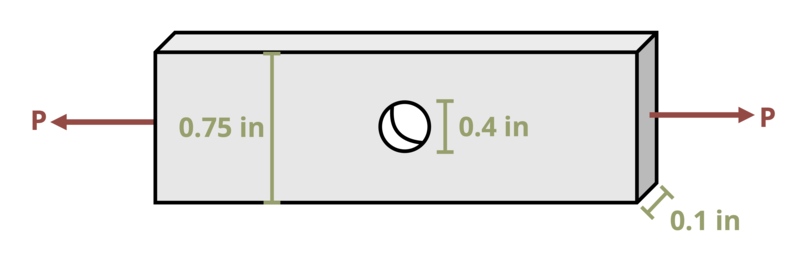
\includegraphics[keepaspectratio]{images/665.png}}
{[}Problem adapted from © Chris Galitz CC BY NC-SA 4.0{]}

\begin{Shaded}
\begin{Highlighting}[]
\NormalTok{\#| standalone: true}
\NormalTok{\#| viewerHeight: 600}
\NormalTok{\#| components: [viewer]}

\NormalTok{from shiny import App, render, ui, reactive}
\NormalTok{import random}
\NormalTok{import asyncio}
\NormalTok{import io}
\NormalTok{import math}
\NormalTok{import string}
\NormalTok{from datetime import datetime}
\NormalTok{from pathlib import Path}

\NormalTok{def generate\_random\_letters(length):}
\NormalTok{    \# Generate a random string of letters of specified length}
\NormalTok{    return \textquotesingle{}\textquotesingle{}.join(random.choice(string.ascii\_lowercase) for \_ in range(length))  }

\NormalTok{problem\_ID="665"}
\NormalTok{t=reactive.Value("\_\_")}
\NormalTok{sigmay=reactive.Value("\_\_")}

\NormalTok{attempts=["Timestamp,Attempt,Answer,Feedback\textbackslash{}n"]}

\NormalTok{app\_ui = ui.page\_fluid(}
\NormalTok{    \#ui.markdown("**Please enter your ID number from your instructor and click to generate your problem**"),}
\NormalTok{    \#ui.input\_text("ID","", placeholder="Enter ID Number Here"),}
\NormalTok{    \#ui.input\_action\_button("generate\_problem", "Generate Problem", class\_="btn{-}primary"),}
\NormalTok{    ui.markdown("**Problem Statement**"),}
\NormalTok{    ui.output\_ui("ui\_problem\_statement"),}
\NormalTok{    ui.input\_text("answer","Your Answer in units of lb", placeholder="Please enter your answer"),}
\NormalTok{    ui.input\_action\_button("submit", "Check Answer", class\_="btn{-}primary"),}
\NormalTok{    \#ui.download\_button("download", "Download File to Submit", class\_="btn{-}success"),}
\NormalTok{)}

\NormalTok{def server(input, output, session):}
\NormalTok{    \# Initialize a counter for attempts}
\NormalTok{    attempt\_counter = reactive.Value(0)}

\NormalTok{    @output}
\NormalTok{    @render.ui}
\NormalTok{    def ui\_problem\_statement():}
\NormalTok{        randomize\_vars()}
\NormalTok{        return[ui.markdown(f"A flat bar of thickness t = \{t()\} in. contains a hole as shown. If the material has a maximum allowable stress of \{sigmay()\} ksi, determine the maximum load P that can be applied.")]}
    
\NormalTok{    \#@reactive.Effect}
\NormalTok{    \#@reactive.event(input.generate\_problem)}
\NormalTok{    def randomize\_vars():}
\NormalTok{        random.seed(101)}
\NormalTok{        t.set(random.randrange(10,50,1)/100)}
\NormalTok{        sigmay.set(random.randrange(20,30,1))}
        
\NormalTok{    @reactive.Effect}
\NormalTok{    @reactive.event(input.submit)}
\NormalTok{    def \_():}
\NormalTok{        attempt\_counter.set(attempt\_counter() + 1)  \# Increment the attempt counter on each submission.}
\NormalTok{        instr=sigmay()*t()*0.35/2.14*1000}
\NormalTok{        if math.isclose(float(input.answer()), instr, rel\_tol=0.01):}
\NormalTok{            check = "*Correct*"}
\NormalTok{            correct\_indicator = "JL"}
\NormalTok{        else:}
\NormalTok{            check = "*Not Correct.*"}
\NormalTok{            correct\_indicator = "JG"}

\NormalTok{        \# Generate random parts for the encoded attempt.}
\NormalTok{        random\_start = generate\_random\_letters(4)}
\NormalTok{        random\_middle = generate\_random\_letters(4)}
\NormalTok{        random\_end = generate\_random\_letters(4)}
\NormalTok{        \#encoded\_attempt = f"\{random\_start\}\{problem\_ID\}{-}\{random\_middle\}\{attempt\_counter()\}\{correct\_indicator\}{-}\{random\_end\}\{input.ID()\}"}

\NormalTok{        \# Store the most recent encoded attempt in a reactive value so it persists across submissions}
\NormalTok{        \#session.encoded\_attempt = reactive.Value(encoded\_attempt)}

\NormalTok{        \# Append the attempt data to the attempts list without the encoded attempt}
\NormalTok{        attempts.append(f"\{datetime.now()\}, \{attempt\_counter()\}, \{input.answer()\}, \{check\}\textbackslash{}n")}

\NormalTok{        \# Show feedback to the user.}
\NormalTok{        feedback = ui.markdown(f"Your answer of \{input.answer()\} is \{check\}.")}
\NormalTok{        m = ui.modal(}
\NormalTok{            feedback,}
\NormalTok{            title="Feedback",}
\NormalTok{            easy\_close=True}
\NormalTok{        )}
\NormalTok{        ui.modal\_show(m)}

\NormalTok{    \#@render.download(filename=lambda: f"Problem\_Log{-}\{problem\_ID\}{-}\{input.ID()\}.csv")}
\NormalTok{    async def download():}
\NormalTok{        \# Start the CSV with the encoded attempt (without label)}
\NormalTok{        final\_encoded = session.encoded\_attempt() if session.encoded\_attempt is not None else "No attempts"}
\NormalTok{        yield f"\{final\_encoded\}\textbackslash{}n\textbackslash{}n"}
        
\NormalTok{        \# Write the header for the remaining CSV data once}
\NormalTok{        yield "Timestamp,Attempt,Answer,Feedback\textbackslash{}n"}
        
\NormalTok{        \# Write the attempts data, ensure that the header from the attempts list is not written again}
\NormalTok{        for attempt in attempts[1:]:  \# Skip the first element which is the header}
\NormalTok{            await asyncio.sleep(0.25)  \# This delay may not be necessary; adjust as needed}
\NormalTok{            yield attempt}

\NormalTok{\# App installation}
\NormalTok{app = App(app\_ui, server)}
\end{Highlighting}
\end{Shaded}

\chapter*{Problem 5.8 - Stress
Concentrations}\label{problem-5.8---stress-concentrations}
\addcontentsline{toc}{chapter}{Problem 5.8 - Stress Concentrations}

\markboth{Problem 5.8 - Stress Concentrations}{Problem 5.8 - Stress
Concentrations}

\begin{figure}[H]

{\centering \pandocbounded{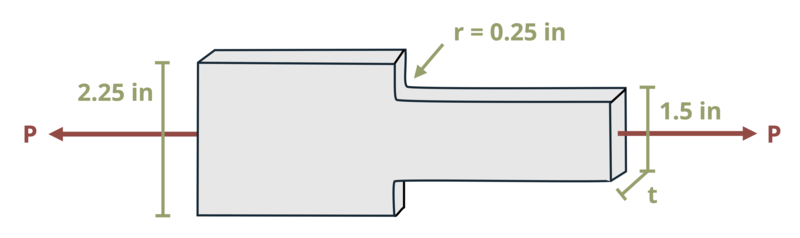
\includegraphics[keepaspectratio]{images/666.png}}

}

\caption{Figure 1: A bar narrows in width.}

\end{figure}%

{[}Problem adapted from © Chris Galitz CC BY NC-SA 4.0{]}

\begin{Shaded}
\begin{Highlighting}[]
\NormalTok{\#| standalone: true}
\NormalTok{\#| viewerHeight: 600}
\NormalTok{\#| components: [viewer]}

\NormalTok{from shiny import App, render, ui, reactive}
\NormalTok{import random}
\NormalTok{import asyncio}
\NormalTok{import io}
\NormalTok{import math}
\NormalTok{import string}
\NormalTok{from datetime import datetime}
\NormalTok{from pathlib import Path}

\NormalTok{def generate\_random\_letters(length):}
\NormalTok{    \# Generate a random string of letters of specified length}
\NormalTok{    return \textquotesingle{}\textquotesingle{}.join(random.choice(string.ascii\_lowercase) for \_ in range(length))  }

\NormalTok{problem\_ID="666"}
\NormalTok{t=reactive.Value("\_\_")}
\NormalTok{P=reactive.Value("\_\_")}

\NormalTok{attempts=["Timestamp,Attempt,Answer,Feedback\textbackslash{}n"]}

\NormalTok{app\_ui = ui.page\_fluid(}
\NormalTok{    \#ui.markdown("**Please enter your ID number from your instructor and click to generate your problem**"),}
\NormalTok{    \#ui.input\_text("ID","", placeholder="Enter ID Number Here"),}
\NormalTok{    \#ui.input\_action\_button("generate\_problem", "Generate Problem", class\_="btn{-}primary"),}
\NormalTok{    ui.markdown("**Problem Statement**"),}
\NormalTok{    ui.output\_ui("ui\_problem\_statement"),}
\NormalTok{    ui.input\_text("answer","Your Answer in units of psi", placeholder="Please enter your answer"),}
\NormalTok{    ui.input\_action\_button("submit", "Check Answer", class\_="btn{-}primary"),}
\NormalTok{    \#ui.download\_button("download", "Download File to Submit", class\_="btn{-}success"),}
\NormalTok{)}

\NormalTok{def server(input, output, session):}
\NormalTok{    \# Initialize a counter for attempts}
\NormalTok{    attempt\_counter = reactive.Value(0)}

\NormalTok{    @output}
\NormalTok{    @render.ui}
\NormalTok{    def ui\_problem\_statement():}
\NormalTok{        randomize\_vars()}
\NormalTok{        return[ui.markdown(f"A flat bar of thickness t = \{t()\} in. narrows with fillets as shown. If a load P = \{P()\} lb is applied, determine the maximum stress in the bar.")]}
    
\NormalTok{    \#@reactive.Effect}
\NormalTok{    \#@reactive.event(input.generate\_problem)}
\NormalTok{    def randomize\_vars():}
\NormalTok{        random.seed(101)}
\NormalTok{        t.set(random.randrange(10, 100, 5)/100)}
\NormalTok{        P.set(random.randrange(1000, 5000, 100))}
        
\NormalTok{    @reactive.Effect}
\NormalTok{    @reactive.event(input.submit)}
\NormalTok{    def \_():}
\NormalTok{        attempt\_counter.set(attempt\_counter() + 1)  \# Increment the attempt counter on each submission.}
\NormalTok{        sigma\_norm = P()/(t()*(1.5))}
\NormalTok{        instr= 1.95*(sigma\_norm)}
\NormalTok{        if math.isclose(float(input.answer()), instr, rel\_tol=0.1):}
\NormalTok{            check = "*Correct*"}
\NormalTok{            correct\_indicator = "JL"}
\NormalTok{        else:}
\NormalTok{            check = "*Not Correct.*"}
\NormalTok{            correct\_indicator = "JG"}

\NormalTok{        \# Generate random parts for the encoded attempt.}
\NormalTok{        random\_start = generate\_random\_letters(4)}
\NormalTok{        random\_middle = generate\_random\_letters(4)}
\NormalTok{        random\_end = generate\_random\_letters(4)}
\NormalTok{        \#encoded\_attempt = f"\{random\_start\}\{problem\_ID\}{-}\{random\_middle\}\{attempt\_counter()\}\{correct\_indicator\}{-}\{random\_end\}\{input.ID()\}"}

\NormalTok{        \# Store the most recent encoded attempt in a reactive value so it persists across submissions}
\NormalTok{        \#session.encoded\_attempt = reactive.Value(encoded\_attempt)}

\NormalTok{        \# Append the attempt data to the attempts list without the encoded attempt}
\NormalTok{        attempts.append(f"\{datetime.now()\}, \{attempt\_counter()\}, \{input.answer()\}, \{check\}\textbackslash{}n")}

\NormalTok{        \# Show feedback to the user.}
\NormalTok{        feedback = ui.markdown(f"Your answer of \{input.answer()\} is \{check\}.")}
\NormalTok{        m = ui.modal(}
\NormalTok{            feedback,}
\NormalTok{            title="Feedback",}
\NormalTok{            easy\_close=True}
\NormalTok{        )}
\NormalTok{        ui.modal\_show(m)}

\NormalTok{    \#@render.download(filename=lambda: f"Problem\_Log{-}\{problem\_ID\}{-}\{input.ID()\}.csv")}
\NormalTok{    async def download():}
\NormalTok{        \# Start the CSV with the encoded attempt (without label)}
\NormalTok{        final\_encoded = session.encoded\_attempt() if session.encoded\_attempt is not None else "No attempts"}
\NormalTok{        yield f"\{final\_encoded\}\textbackslash{}n\textbackslash{}n"}
        
\NormalTok{        \# Write the header for the remaining CSV data once}
\NormalTok{        yield "Timestamp,Attempt,Answer,Feedback\textbackslash{}n"}
        
\NormalTok{        \# Write the attempts data, ensure that the header from the attempts list is not written again}
\NormalTok{        for attempt in attempts[1:]:  \# Skip the first element which is the header}
\NormalTok{            await asyncio.sleep(0.25)  \# This delay may not be necessary; adjust as needed}
\NormalTok{            yield attempt}

\NormalTok{\# App installation}
\NormalTok{app = App(app\_ui, server)}
\end{Highlighting}
\end{Shaded}

\chapter*{Problem 5.9 - Stress
Concentrations}\label{problem-5.9---stress-concentrations}
\addcontentsline{toc}{chapter}{Problem 5.9 - Stress Concentrations}

\markboth{Problem 5.9 - Stress Concentrations}{Problem 5.9 - Stress
Concentrations}

\pandocbounded{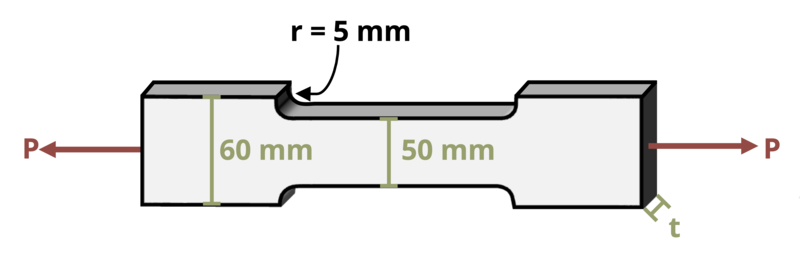
\includegraphics[keepaspectratio]{images/667.png}}
{[}Problem adapted from © Chris Galitz CC BY NC-SA 4.0{]}

\begin{Shaded}
\begin{Highlighting}[]
\NormalTok{\#| standalone: true}
\NormalTok{\#| viewerHeight: 600}
\NormalTok{\#| components: [viewer]}

\NormalTok{from shiny import App, render, ui, reactive}
\NormalTok{import random}
\NormalTok{import asyncio}
\NormalTok{import io}
\NormalTok{import math}
\NormalTok{import string}
\NormalTok{from datetime import datetime}
\NormalTok{from pathlib import Path}

\NormalTok{def generate\_random\_letters(length):}
\NormalTok{    \# Generate a random string of letters of specified length}
\NormalTok{    return \textquotesingle{}\textquotesingle{}.join(random.choice(string.ascii\_lowercase) for \_ in range(length))  }

\NormalTok{problem\_ID="667"}
\NormalTok{t=reactive.Value("\_\_")}
\NormalTok{P=reactive.Value("\_\_")}
  
\NormalTok{attempts=["Timestamp,Attempt,Answer,Feedback\textbackslash{}n"]}

\NormalTok{app\_ui = ui.page\_fluid(}
\NormalTok{    \#ui.markdown("**Please enter your ID number from your instructor and click to generate your problem**"),}
\NormalTok{    \#ui.input\_text("ID","", placeholder="Enter ID Number Here"),}
\NormalTok{    \#ui.input\_action\_button("generate\_problem", "Generate Problem", class\_="btn{-}primary"),}
\NormalTok{    ui.markdown("**Problem Statement**"),}
\NormalTok{    ui.output\_ui("ui\_problem\_statement"),}
\NormalTok{    ui.input\_text("answer","Your Answer in units of MPa", placeholder="Please enter your answer"),}
\NormalTok{    ui.input\_action\_button("submit", "Check Answer", class\_="btn{-}primary"),}
\NormalTok{    \#ui.download\_button("download", "Download File to Submit", class\_="btn{-}success"),}
\NormalTok{)}

\NormalTok{def server(input, output, session):}
\NormalTok{    \# Initialize a counter for attempts}
\NormalTok{    attempt\_counter = reactive.Value(0)}

\NormalTok{    @output}
\NormalTok{    @render.ui}
\NormalTok{    def ui\_problem\_statement():}
\NormalTok{        randomize\_vars()}
\NormalTok{        return[ui.markdown(f"A dogbone specimen of thickness t = \{t()\} mm is being prepared for a tension test. If load P = \{P()\} kN, determine the maximum stress in the sample.")]}
    
\NormalTok{    \#@reactive.Effect}
\NormalTok{    \#@reactive.event(input.generate\_problem)}
\NormalTok{    def randomize\_vars():}
\NormalTok{        random.seed(101)}
\NormalTok{        t.set(random.randrange(70,200,1)/10)}
\NormalTok{        P.set(random.randrange(20,50,1))}

\NormalTok{    @reactive.Effect}
\NormalTok{    @reactive.event(input.submit)}
\NormalTok{    def \_():}
\NormalTok{        attempt\_counter.set(attempt\_counter() + 1)  \# Increment the attempt counter on each submission.}
\NormalTok{        A = 0.05*t()}
\NormalTok{        sigmaavg=P()/A}
\NormalTok{        instr= sigmaavg*1.88}
\NormalTok{        if math.isclose(float(input.answer()), instr, rel\_tol=0.03):}
\NormalTok{            check = "*Correct*"}
\NormalTok{            correct\_indicator = "JL"}
\NormalTok{        else:}
\NormalTok{            check = "*Not Correct.*"}
\NormalTok{            correct\_indicator = "JG"}

\NormalTok{        \# Generate random parts for the encoded attempt.}
\NormalTok{        random\_start = generate\_random\_letters(4)}
\NormalTok{        random\_middle = generate\_random\_letters(4)}
\NormalTok{        random\_end = generate\_random\_letters(4)}
\NormalTok{        \#encoded\_attempt = f"\{random\_start\}\{problem\_ID\}{-}\{random\_middle\}\{attempt\_counter()\}\{correct\_indicator\}{-}\{random\_end\}\{input.ID()\}"}

\NormalTok{        \# Store the most recent encoded attempt in a reactive value so it persists across submissions}
\NormalTok{        \#session.encoded\_attempt = reactive.Value(encoded\_attempt)}

\NormalTok{        \# Append the attempt data to the attempts list without the encoded attempt}
\NormalTok{        attempts.append(f"\{datetime.now()\}, \{attempt\_counter()\}, \{input.answer()\}, \{check\}\textbackslash{}n")}

\NormalTok{        \# Show feedback to the user.}
\NormalTok{        feedback = ui.markdown(f"Your answer of \{input.answer()\} is \{check\}.")}
\NormalTok{        m = ui.modal(}
\NormalTok{            feedback,}
\NormalTok{            title="Feedback",}
\NormalTok{            easy\_close=True}
\NormalTok{        )}
\NormalTok{        ui.modal\_show(m)}

\NormalTok{    \#@render.download(filename=lambda: f"Problem\_Log{-}\{problem\_ID\}{-}\{input.ID()\}.csv")}
\NormalTok{    async def download():}
\NormalTok{        \# Start the CSV with the encoded attempt (without label)}
\NormalTok{        final\_encoded = session.encoded\_attempt() if session.encoded\_attempt is not None else "No attempts"}
\NormalTok{        yield f"\{final\_encoded\}\textbackslash{}n\textbackslash{}n"}
        
\NormalTok{        \# Write the header for the remaining CSV data once}
\NormalTok{        yield "Timestamp,Attempt,Answer,Feedback\textbackslash{}n"}
        
\NormalTok{        \# Write the attempts data, ensure that the header from the attempts list is not written again}
\NormalTok{        for attempt in attempts[1:]:  \# Skip the first element which is the header}
\NormalTok{            await asyncio.sleep(0.25)  \# This delay may not be necessary; adjust as needed}
\NormalTok{            yield attempt}


\NormalTok{\# App installation}
\NormalTok{app = App(app\_ui, server)}
\end{Highlighting}
\end{Shaded}

\chapter*{Problem 5.10 - Stress
Concentrations}\label{problem-5.10---stress-concentrations}
\addcontentsline{toc}{chapter}{Problem 5.10 - Stress Concentrations}

\markboth{Problem 5.10 - Stress Concentrations}{Problem 5.10 - Stress
Concentrations}

\begin{figure}[H]

{\centering \pandocbounded{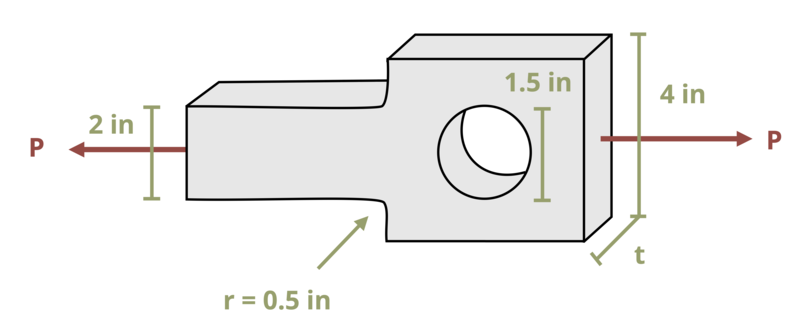
\includegraphics[keepaspectratio]{images/668.png}}

}

\caption{Figure 1: A linkage is subjected to a loading as shown.}

\end{figure}%

{[}Problem adapted from © Chris Galitz CC BY NC-SA 4.0{]}

\begin{Shaded}
\begin{Highlighting}[]
\NormalTok{\#| standalone: true}
\NormalTok{\#| viewerHeight: 600}
\NormalTok{\#| components: [viewer]}

\NormalTok{from shiny import App, render, ui, reactive}
\NormalTok{import random}
\NormalTok{import asyncio}
\NormalTok{import io}
\NormalTok{import math}
\NormalTok{import string}
\NormalTok{from datetime import datetime}
\NormalTok{from pathlib import Path}

\NormalTok{def generate\_random\_letters(length):}
\NormalTok{    \# Generate a random string of letters of specified length}
\NormalTok{    return \textquotesingle{}\textquotesingle{}.join(random.choice(string.ascii\_lowercase) for \_ in range(length))  }

\NormalTok{problem\_ID="668"}
\NormalTok{t=reactive.Value("\_\_")}
\NormalTok{P=reactive.Value("\_\_")}
  
\NormalTok{attempts=["Timestamp,Attempt,Answer,Feedback\textbackslash{}n"]}

\NormalTok{app\_ui = ui.page\_fluid(}
\NormalTok{    \#ui.markdown("**Please enter your ID number from your instructor and click to generate your problem**"),}
\NormalTok{    \#ui.input\_text("ID","", placeholder="Enter ID Number Here"),}
\NormalTok{    \#ui.input\_action\_button("generate\_problem", "Generate Problem", class\_="btn{-}primary"),}
\NormalTok{    ui.markdown("**Problem Statement**"),}
\NormalTok{    ui.output\_ui("ui\_problem\_statement"),}
\NormalTok{    ui.input\_text("answer","Your Answer in units of ksi", placeholder="Please enter your answer"),}
\NormalTok{    ui.input\_action\_button("submit", "Check Answer", class\_="btn{-}primary"),}
\NormalTok{    \#ui.download\_button("download", "Download File to Submit", class\_="btn{-}success"),}
\NormalTok{)}

\NormalTok{def server(input, output, session):}
\NormalTok{    \# Initialize a counter for attempts}
\NormalTok{    attempt\_counter = reactive.Value(0)}

\NormalTok{    @output}
\NormalTok{    @render.ui}
\NormalTok{    def ui\_problem\_statement():}
\NormalTok{        randomize\_vars()}
\NormalTok{        return[ui.markdown(f"The linkage of thickness t = \{t()\} in. shown is subjected to load P = \{P()\} kips. Determine the maximum stress in the linkage.")]}
    
\NormalTok{    \#@reactive.Effect}
\NormalTok{    \#@reactive.event(input.generate\_problem)}
\NormalTok{    def randomize\_vars():}
\NormalTok{        random.seed(101)}
\NormalTok{        t.set(random.randrange(25, 75, 5)/100)}
\NormalTok{        P.set(random.randrange(20,45,1))}

\NormalTok{    @reactive.Effect}
\NormalTok{    @reactive.event(input.submit)}
\NormalTok{    def \_():}
\NormalTok{        attempt\_counter.set(attempt\_counter() + 1)  \# Increment the attempt counter on each submission.}
\NormalTok{        sigma1 = 1.82*P()/(2*t())}
\NormalTok{        sigma2 = 2.28*P()/(2.5*t())}
\NormalTok{        instr = max(sigma1,sigma2)}
        
\NormalTok{        if math.isclose(float(input.answer()), instr, rel\_tol=0.1):}
\NormalTok{            check = "*Correct*"}
\NormalTok{            correct\_indicator = "JL"}
\NormalTok{        else:}
\NormalTok{            check = "*Not Correct.*"}
\NormalTok{            correct\_indicator = "JG"}

\NormalTok{        \# Generate random parts for the encoded attempt.}
\NormalTok{        random\_start = generate\_random\_letters(4)}
\NormalTok{        random\_middle = generate\_random\_letters(4)}
\NormalTok{        random\_end = generate\_random\_letters(4)}
\NormalTok{        \#encoded\_attempt = f"\{random\_start\}\{problem\_ID\}{-}\{random\_middle\}\{attempt\_counter()\}\{correct\_indicator\}{-}\{random\_end\}\{input.ID()\}"}

\NormalTok{        \# Store the most recent encoded attempt in a reactive value so it persists across submissions}
\NormalTok{        \#session.encoded\_attempt = reactive.Value(encoded\_attempt)}

\NormalTok{        \# Append the attempt data to the attempts list without the encoded attempt}
\NormalTok{        attempts.append(f"\{datetime.now()\}, \{attempt\_counter()\}, \{input.answer()\}, \{check\}\textbackslash{}n")}

\NormalTok{        \# Show feedback to the user.}
\NormalTok{        feedback = ui.markdown(f"Your answer of \{input.answer()\} is \{check\}.")}
\NormalTok{        m = ui.modal(}
\NormalTok{            feedback,}
\NormalTok{            title="Feedback",}
\NormalTok{            easy\_close=True}
\NormalTok{        )}
\NormalTok{        ui.modal\_show(m)}

\NormalTok{    \#@render.download(filename=lambda: f"Problem\_Log{-}\{problem\_ID\}{-}\{input.ID()\}.csv")}
\NormalTok{    async def download():}
\NormalTok{        \# Start the CSV with the encoded attempt (without label)}
\NormalTok{        final\_encoded = session.encoded\_attempt() if session.encoded\_attempt is not None else "No attempts"}
\NormalTok{        yield f"\{final\_encoded\}\textbackslash{}n\textbackslash{}n"}
        
\NormalTok{        \# Write the header for the remaining CSV data once}
\NormalTok{        yield "Timestamp,Attempt,Answer,Feedback\textbackslash{}n"}
        
\NormalTok{        \# Write the attempts data, ensure that the header from the attempts list is not written again}
\NormalTok{        for attempt in attempts[1:]:  \# Skip the first element which is the header}
\NormalTok{            await asyncio.sleep(0.25)  \# This delay may not be necessary; adjust as needed}
\NormalTok{            yield attempt}
            
\NormalTok{\# App installation}
\NormalTok{app = App(app\_ui, server)}
\end{Highlighting}
\end{Shaded}

\chapter*{Problem 5.11 - Axial
Deformation}\label{problem-5.11---axial-deformation}
\addcontentsline{toc}{chapter}{Problem 5.11 - Axial Deformation}

\markboth{Problem 5.11 - Axial Deformation}{Problem 5.11 - Axial
Deformation}

\pandocbounded{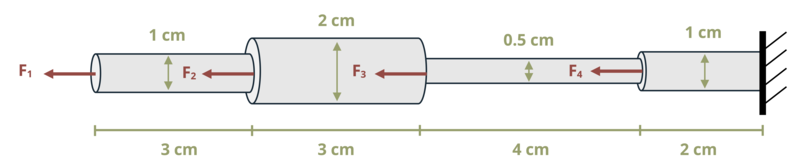
\includegraphics[keepaspectratio]{images/183.png}}
{[}Problem adapted from © Kurt Gramoll CC BY NC-SA 4.0{]}

\begin{Shaded}
\begin{Highlighting}[]
\NormalTok{\#| standalone: true}
\NormalTok{\#| viewerHeight: 600}
\NormalTok{\#| components: [viewer]}

\NormalTok{from shiny import App, render, ui, reactive}
\NormalTok{import random}
\NormalTok{import asyncio}
\NormalTok{import io}
\NormalTok{import math}
\NormalTok{import string}
\NormalTok{from datetime import datetime}
\NormalTok{from pathlib import Path}

\NormalTok{problem\_ID="183"}
\NormalTok{F1=reactive.Value("\_\_")}
\NormalTok{F2=reactive.Value("\_\_")}
\NormalTok{F3=reactive.Value("\_\_")}
\NormalTok{F4=reactive.Value("\_\_")}
\NormalTok{E=210}

\NormalTok{def generate\_random\_letters(length):}
\NormalTok{    \# Generate a random string of letters of specified length}
\NormalTok{    return \textquotesingle{}\textquotesingle{}.join(random.choice(string.ascii\_lowercase) for \_ in range(length))  }

\NormalTok{attempts=["Timestamp,Attempt,Answer,Feedback\textbackslash{}n"]}

\NormalTok{app\_ui = ui.page\_fluid(}
\NormalTok{    \#ui.markdown("**Please enter your ID number from your instructor and click to generate your problem**"),}
\NormalTok{    \#ui.input\_text("ID","", placeholder="Enter ID Number Here"),}
\NormalTok{    \#ui.input\_action\_button("generate\_problem", "Generate Problem", class\_="btn{-}primary"),}
\NormalTok{    ui.markdown("**Problem Statement**"),}
\NormalTok{    ui.output\_ui("ui\_problem\_statement"),}
\NormalTok{    ui.input\_text("answer","Your Answer in units of mm", placeholder="Please enter your answer"),}
\NormalTok{    ui.input\_action\_button("submit", "Check Answer", class\_="btn{-}primary"),}
\NormalTok{    \#ui.download\_button("download", "Download File to Submit", class\_="btn{-}success"),}
\NormalTok{)}

\NormalTok{def server(input, output, session):}
\NormalTok{    \# Initialize a counter for attempts}
\NormalTok{    attempt\_counter = reactive.Value(0)}

\NormalTok{    @output}
\NormalTok{    @render.ui}
\NormalTok{    def ui\_problem\_statement():}
\NormalTok{        randomize\_vars()}
\NormalTok{        return[ui.markdown(f"A series of solid, steel, circular bars are loaded with forces as shown, where F\textless{}sub\textgreater{}1\textless{}/sub\textgreater{} = \{F1()\} kN, F\textless{}sub\textgreater{}2\textless{}/sub\textgreater{} = \{F2()\} kN, F\textless{}sub\textgreater{}3\textless{}/sub\textgreater{} = \{F3()\} kN, and F\textless{}sub\textgreater{}4\textless{}/sub\textgreater{} = \{F4()\} kN. What is the total change in length of the system? Assume E = 210 GPa for steel.")]}
    
\NormalTok{    \#@reactive.Effect}
\NormalTok{    \#@reactive.event(input.generate\_problem)}
\NormalTok{    def randomize\_vars():}
\NormalTok{        random.seed(101)}
\NormalTok{        F1.set(random.randrange(10, 100, 1)/10)}
\NormalTok{        F2.set(random.randrange(10, 100, 1)/10)}
\NormalTok{        F3.set(random.randrange(10, 100, 1)/10)}
\NormalTok{        F4.set(random.randrange(10, 100, 1)/10)}

\NormalTok{    @reactive.Effect}
\NormalTok{    @reactive.event(input.submit)}
\NormalTok{    def \_():}
\NormalTok{        attempt\_counter.set(attempt\_counter() + 1)  \# Increment the attempt counter on each submission.}
\NormalTok{        instr= ((F1()*3)/(E*math.pi*0.5**2)+((F1()+F2())*3)/(E*math.pi*1**2)+((F1()+F2()+F3())*4)/(E*math.pi*0.25**2)+((F1()+F2()+F3()+F4())*2)/(E*math.pi*0.5**2))/10}
\NormalTok{        if math.isclose(float(input.answer()), instr, rel\_tol=0.01):}
\NormalTok{            check = "*Correct*"}
\NormalTok{            correct\_indicator = "JL"}
\NormalTok{        else:}
\NormalTok{            check = "*Not Correct.*"}
\NormalTok{            correct\_indicator = "JG"}

\NormalTok{        \# Generate random parts for the encoded attempt.}
\NormalTok{        random\_start = generate\_random\_letters(4)}
\NormalTok{        random\_middle = generate\_random\_letters(4)}
\NormalTok{        random\_end = generate\_random\_letters(4)}
\NormalTok{        \#encoded\_attempt = f"\{random\_start\}\{problem\_ID\}{-}\{random\_middle\}\{attempt\_counter()\}\{correct\_indicator\}{-}\{random\_end\}\{input.ID()\}"}

\NormalTok{        \# Store the most recent encoded attempt in a reactive value so it persists across submissions}
\NormalTok{        \#session.encoded\_attempt = reactive.Value(encoded\_attempt)}

\NormalTok{        \# Append the attempt data to the attempts list without the encoded attempt}
\NormalTok{        attempts.append(f"\{datetime.now()\}, \{attempt\_counter()\}, \{input.answer()\}, \{check\}\textbackslash{}n")}

\NormalTok{        \# Show feedback to the user.}
\NormalTok{        feedback = ui.markdown(f"Your answer of \{input.answer()\} is \{check\}.")}
\NormalTok{        m = ui.modal(}
\NormalTok{            feedback,}
\NormalTok{            title="Feedback",}
\NormalTok{            easy\_close=True}
\NormalTok{        )}
\NormalTok{        ui.modal\_show(m)}

\NormalTok{    \#@render.download(filename=lambda: f"Problem\_Log{-}\{problem\_ID\}{-}\{input.ID()\}.csv")}
\NormalTok{    async def download():}
\NormalTok{        \# Start the CSV with the encoded attempt (without label)}
\NormalTok{        final\_encoded = session.encoded\_attempt() if session.encoded\_attempt is not None else "No attempts"}
\NormalTok{        yield f"\{final\_encoded\}\textbackslash{}n\textbackslash{}n"}
        
\NormalTok{        \# Write the header for the remaining CSV data once}
\NormalTok{        yield "Timestamp,Attempt,Answer,Feedback\textbackslash{}n"}
        
\NormalTok{        \# Write the attempts data, ensure that the header from the attempts list is not written again}
\NormalTok{        for attempt in attempts[1:]:  \# Skip the first element which is the header}
\NormalTok{            await asyncio.sleep(0.25)  \# This delay may not be necessary; adjust as needed}
\NormalTok{            yield attempt}

\NormalTok{\# App installation}
\NormalTok{app = App(app\_ui, server)}
\end{Highlighting}
\end{Shaded}

\chapter*{Problem 5.12 - Axial
Deformation}\label{problem-5.12---axial-deformation}
\addcontentsline{toc}{chapter}{Problem 5.12 - Axial Deformation}

\markboth{Problem 5.12 - Axial Deformation}{Problem 5.12 - Axial
Deformation}

\pandocbounded{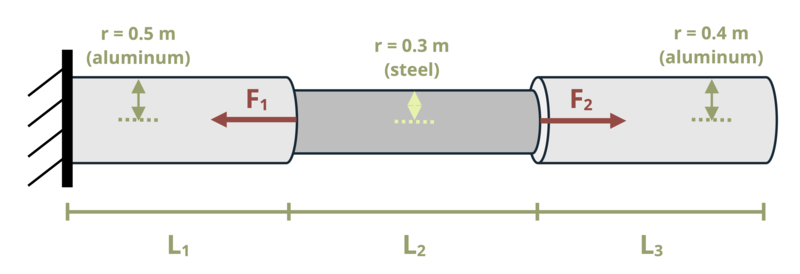
\includegraphics[keepaspectratio]{images/184.png}}
{[}Problem adapted from © Kurt Gramoll CC BY NC-SA 4.0{]}

\begin{Shaded}
\begin{Highlighting}[]
\NormalTok{\#| standalone: true}
\NormalTok{\#| viewerHeight: 600}
\NormalTok{\#| components: [viewer]}

\NormalTok{from shiny import App, render, ui, reactive}
\NormalTok{import random}
\NormalTok{import asyncio}
\NormalTok{import io}
\NormalTok{import math}
\NormalTok{import string}
\NormalTok{from datetime import datetime}
\NormalTok{from pathlib import Path}

\NormalTok{def generate\_random\_letters(length):}
\NormalTok{    \# Generate a random string of letters of specified length}
\NormalTok{    return \textquotesingle{}\textquotesingle{}.join(random.choice(string.ascii\_lowercase) for \_ in range(length)) }

\NormalTok{problem\_ID="184"}
\NormalTok{F1=reactive.Value("\_\_")}
\NormalTok{F2=reactive.Value("\_\_")}
\NormalTok{L1=reactive.Value("\_\_")}
\NormalTok{L2=reactive.Value("\_\_")}
\NormalTok{L3=reactive.Value("\_\_")}
\NormalTok{Esteel = 210}
\NormalTok{Ealuminum = 70}

\NormalTok{attempts=["Timestamp,Attempt,Answer,Feedback\textbackslash{}n"]}

\NormalTok{app\_ui = ui.page\_fluid(}
\NormalTok{    \#ui.markdown("**Please enter your ID number from your instructor and click to generate your problem**"),}
\NormalTok{    \#ui.input\_text("ID","", placeholder="Enter ID Number Here"),}
\NormalTok{    \#ui.input\_action\_button("generate\_problem", "Generate Problem", class\_="btn{-}primary"),}
\NormalTok{    ui.markdown("**Problem Statement**"),}
\NormalTok{    ui.output\_ui("ui\_problem\_statement"),}
\NormalTok{    ui.input\_text("answer","Your Answer in units of micrometers", placeholder="Please enter your answer"),}
\NormalTok{    ui.input\_action\_button("submit", "Check Answer", class\_="btn{-}primary"),}
\NormalTok{    \#ui.download\_button("download", "Download File to Submit", class\_="btn{-}success"),}
\NormalTok{)}

\NormalTok{def server(input, output, session):}
\NormalTok{    \# Initialize a counter for attempts}
\NormalTok{    attempt\_counter = reactive.Value(0)}

\NormalTok{    @output}
\NormalTok{    @render.ui}
\NormalTok{    def ui\_problem\_statement():}
\NormalTok{        randomize\_vars()}
\NormalTok{        return[ui.markdown(f"Two forces, F\textless{}sub\textgreater{}1\textless{}/sub\textgreater{} = \{F1()\} kN and F\textless{}sub\textgreater{}2\textless{}/sub\textgreater{} = \{F2()\} kN, are applied to the system of cylinders as shown. If L\textless{}sub\textgreater{}1\textless{}/sub\textgreater{} = \{L1()\} m, L\textless{}sub\textgreater{}2\textless{}/sub\textgreater{} = \{L2()\} m, and L\textless{}sub\textgreater{}3\textless{}/sub\textgreater{} = \{L3()\} m, what is the total change in length of the system? Assume E\textless{}sub\textgreater{}steel\textless{}/sub\textgreater{} = \{Esteel\} GPa and E\textless{}sub\textgreater{}aluminum\textless{}/sub\textgreater{} = \{Ealuminum\} GPa.")]}
    
\NormalTok{    \#@reactive.Effect}
\NormalTok{    \#@reactive.event(input.generate\_problem)}
\NormalTok{    def randomize\_vars():}
\NormalTok{        random.seed(101)}
\NormalTok{        F1.set(random.randrange(100, 300, 1)/10)}
\NormalTok{        F2.set(round(F1()/1.5, 2))}
\NormalTok{        L1.set(random.randrange(20, 80, 1)/10)}
\NormalTok{        L2.set(round(L1()*0.6, 2))}
\NormalTok{        L3.set(round(L1()*0.8, 2))}
        
\NormalTok{    @reactive.Effect}
\NormalTok{    @reactive.event(input.submit)}
\NormalTok{    def \_():}
\NormalTok{        attempt\_counter.set(attempt\_counter() + 1)  \# Increment the attempt counter on each submission.}
       
\NormalTok{        instr= ((F2()*10**3*L2())/(math.pi*0.3**2*Esteel*10**9) + ((F2(){-}F1())*1000*L1())/(math.pi*0.5**2*Ealuminum*10**9))*1000000}
\NormalTok{        if math.isclose(float(input.answer()), instr, rel\_tol=0.01):}
\NormalTok{            check = "*Correct*"}
\NormalTok{            correct\_indicator = "JL"}
\NormalTok{        else:}
\NormalTok{            check = "*Not Correct.*"}
\NormalTok{            correct\_indicator = "JG"}

\NormalTok{        \# Generate random parts for the encoded attempt.}
\NormalTok{        random\_start = generate\_random\_letters(4)}
\NormalTok{        random\_middle = generate\_random\_letters(4)}
\NormalTok{        random\_end = generate\_random\_letters(4)}
\NormalTok{        \#encoded\_attempt = f"\{random\_start\}\{problem\_ID\}{-}\{random\_middle\}\{attempt\_counter()\}\{correct\_indicator\}{-}\{random\_end\}\{input.ID()\}"}

\NormalTok{        \# Store the most recent encoded attempt in a reactive value so it persists across submissions}
\NormalTok{        \#session.encoded\_attempt = reactive.Value(encoded\_attempt)}

\NormalTok{        \# Append the attempt data to the attempts list without the encoded attempt}
\NormalTok{        attempts.append(f"\{datetime.now()\}, \{attempt\_counter()\}, \{input.answer()\}, \{check\}\textbackslash{}n")}

\NormalTok{        \# Show feedback to the user.}
\NormalTok{        feedback = ui.markdown(f"Your answer of \{input.answer()\} is \{check\}.")}
\NormalTok{        m = ui.modal(}
\NormalTok{            feedback,}
\NormalTok{            title="Feedback",}
\NormalTok{            easy\_close=True}
\NormalTok{        )}
\NormalTok{        ui.modal\_show(m)}

\NormalTok{    \#@render.download(filename=lambda: f"Problem\_Log{-}\{problem\_ID\}{-}\{input.ID()\}.csv")}
\NormalTok{    async def download():}
\NormalTok{        \# Start the CSV with the encoded attempt (without label)}
\NormalTok{        final\_encoded = session.encoded\_attempt() if session.encoded\_attempt is not None else "No attempts"}
\NormalTok{        yield f"\{final\_encoded\}\textbackslash{}n\textbackslash{}n"}
        
\NormalTok{        \# Write the header for the remaining CSV data once}
\NormalTok{        yield "Timestamp,Attempt,Answer,Feedback\textbackslash{}n"}
        
\NormalTok{        \# Write the attempts data, ensure that the header from the attempts list is not written again}
\NormalTok{        for attempt in attempts[1:]:  \# Skip the first element which is the header}
\NormalTok{            await asyncio.sleep(0.25)  \# This delay may not be necessary; adjust as needed}
\NormalTok{            yield attempt}

\NormalTok{\# App installation}
\NormalTok{app = App(app\_ui, server)}
\end{Highlighting}
\end{Shaded}

\chapter*{Problem 5.13 - Axial
Deformation}\label{problem-5.13---axial-deformation}
\addcontentsline{toc}{chapter}{Problem 5.13 - Axial Deformation}

\markboth{Problem 5.13 - Axial Deformation}{Problem 5.13 - Axial
Deformation}

\pandocbounded{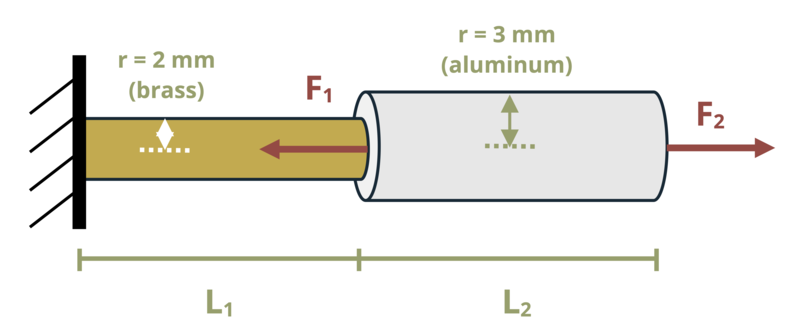
\includegraphics[keepaspectratio]{images/185.png}}
{[}Problem adapted from © Kurt Gramoll CC BY NC-SA 4.0{]}

\begin{Shaded}
\begin{Highlighting}[]
\NormalTok{\#| standalone: true}
\NormalTok{\#| viewerHeight: 600}
\NormalTok{\#| components: [viewer]}

\NormalTok{from shiny import App, render, ui, reactive}
\NormalTok{import random}
\NormalTok{import asyncio}
\NormalTok{import io}
\NormalTok{import math}
\NormalTok{import string}
\NormalTok{from datetime import datetime}
\NormalTok{from pathlib import Path}

\NormalTok{def generate\_random\_letters(length):}
\NormalTok{    \# Generate a random string of letters of specified length}
\NormalTok{    return \textquotesingle{}\textquotesingle{}.join(random.choice(string.ascii\_lowercase) for \_ in range(length))}

\NormalTok{problem\_ID="185"}
\NormalTok{F1=reactive.Value("\_\_")}
\NormalTok{F2=reactive.Value("\_\_")}
\NormalTok{L1=reactive.Value("\_\_")}
\NormalTok{L2=reactive.Value("\_\_")}
\NormalTok{Ebrass = 100}
\NormalTok{Ealuminum = 70}

\NormalTok{attempts=["Timestamp,Attempt,Answer,Feedback\textbackslash{}n"]}

\NormalTok{app\_ui = ui.page\_fluid(}
\NormalTok{    \#ui.markdown("**Please enter your ID number from your instructor and click to generate your problem**"),}
\NormalTok{    \#ui.input\_text("ID","", placeholder="Enter ID Number Here"),}
\NormalTok{    \#ui.input\_action\_button("generate\_problem", "Generate Problem", class\_="btn{-}primary"),}
\NormalTok{    ui.markdown("**Problem Statement**"),}
\NormalTok{    ui.output\_ui("ui\_problem\_statement"),}
\NormalTok{    ui.input\_text("answer","Your Answer in units of mm", placeholder="Please enter your answer"),}
\NormalTok{    ui.input\_action\_button("submit", "Check Answer", class\_="btn{-}primary"),}
\NormalTok{    \#ui.download\_button("download", "Download File to Submit", class\_="btn{-}success"),}
\NormalTok{)}

\NormalTok{def server(input, output, session):}
\NormalTok{    \# Initialize a counter for attempts}
\NormalTok{    attempt\_counter = reactive.Value(0)}

\NormalTok{    @output}
\NormalTok{    @render.ui}
\NormalTok{    def ui\_problem\_statement():}
\NormalTok{        randomize\_vars()}
\NormalTok{        return[ui.markdown(f"Two forces, F\textless{}sub\textgreater{}1\textless{}/sub\textgreater{} = \{F1()\} kN and F\textless{}sub\textgreater{}2\textless{}/sub\textgreater{} = \{F2()\} kN, are applied to the system of cylinders as shown. If L\textless{}sub\textgreater{}1\textless{}/sub\textgreater{} = \{L1()\} mm and L\textless{}sub\textgreater{}2\textless{}/sub\textgreater{} = \{L2()\} mm, what is the total change in length of the system. Assume E\textless{}sub\textgreater{}brass\textless{}/sub\textgreater{} = \{Ebrass\} GPa and E\textless{}sub\textgreater{}aluminum\textless{}/sub\textgreater{} = \{Ealuminum\} GPa.")]}
    
\NormalTok{    \#@reactive.Effect}
\NormalTok{    \#@reactive.event(input.generate\_problem)}
\NormalTok{    def randomize\_vars():}
\NormalTok{        random.seed(101)}
\NormalTok{        F1.set(random.randrange(10, 100, 1)/10)}
\NormalTok{        F2.set(round(F1()*2, 2))}
\NormalTok{        L1.set(random.randrange(50, 150, 1))}
\NormalTok{        L2.set(round(L1()*1.5))}
        
\NormalTok{    @reactive.Effect}
\NormalTok{    @reactive.event(input.submit)}
\NormalTok{    def \_():}
\NormalTok{        attempt\_counter.set(attempt\_counter() + 1)  \# Increment the attempt counter on each submission.}
\NormalTok{        instr= (((F2(){-}F1())*L1())/(math.pi*.002**2*Ebrass*10**6)) + (F2()*L2())/(math.pi*.003**2*Ealuminum*10**6)}
\NormalTok{        if math.isclose(float(input.answer()), instr, rel\_tol=0.01):}
\NormalTok{            check = "*Correct*"}
\NormalTok{            correct\_indicator = "JL"}
\NormalTok{        else:}
\NormalTok{            check = "*Not Correct.*"}
\NormalTok{            correct\_indicator = "JG"}

\NormalTok{        \# Generate random parts for the encoded attempt.}
\NormalTok{        random\_start = generate\_random\_letters(4)}
\NormalTok{        random\_middle = generate\_random\_letters(4)}
\NormalTok{        random\_end = generate\_random\_letters(4)}
\NormalTok{        \#encoded\_attempt = f"\{random\_start\}\{problem\_ID\}{-}\{random\_middle\}\{attempt\_counter()\}\{correct\_indicator\}{-}\{random\_end\}\{input.ID()\}"}

\NormalTok{        \# Store the most recent encoded attempt in a reactive value so it persists across submissions}
\NormalTok{        \#session.encoded\_attempt = reactive.Value(encoded\_attempt)}

\NormalTok{        \# Append the attempt data to the attempts list without the encoded attempt}
\NormalTok{        attempts.append(f"\{datetime.now()\}, \{attempt\_counter()\}, \{input.answer()\}, \{check\}\textbackslash{}n")}

\NormalTok{        \# Show feedback to the user.}
\NormalTok{        feedback = ui.markdown(f"Your answer of \{input.answer()\} is \{check\}.")}
\NormalTok{        m = ui.modal(}
\NormalTok{            feedback,}
\NormalTok{            title="Feedback",}
\NormalTok{            easy\_close=True}
\NormalTok{        )}
\NormalTok{        ui.modal\_show(m)}

\NormalTok{    \#@render.download(filename=lambda: f"Problem\_Log{-}\{problem\_ID\}{-}\{input.ID()\}.csv")}
\NormalTok{    async def download():}
\NormalTok{        \# Start the CSV with the encoded attempt (without label)}
\NormalTok{        final\_encoded = session.encoded\_attempt() if session.encoded\_attempt is not None else "No attempts"}
\NormalTok{        yield f"\{final\_encoded\}\textbackslash{}n\textbackslash{}n"}
        
\NormalTok{        \# Write the header for the remaining CSV data once}
\NormalTok{        yield "Timestamp,Attempt,Answer,Feedback\textbackslash{}n"}
        
\NormalTok{        \# Write the attempts data, ensure that the header from the attempts list is not written again}
\NormalTok{        for attempt in attempts[1:]:  \# Skip the first element which is the header}
\NormalTok{            await asyncio.sleep(0.25)  \# This delay may not be necessary; adjust as needed}
\NormalTok{            yield attempt}

\NormalTok{\# App installation}
\NormalTok{app = App(app\_ui, server)}
\end{Highlighting}
\end{Shaded}

\chapter*{Problem 5.14 - Axial
Deformation}\label{problem-5.14---axial-deformation}
\addcontentsline{toc}{chapter}{Problem 5.14 - Axial Deformation}

\markboth{Problem 5.14 - Axial Deformation}{Problem 5.14 - Axial
Deformation}

\pandocbounded{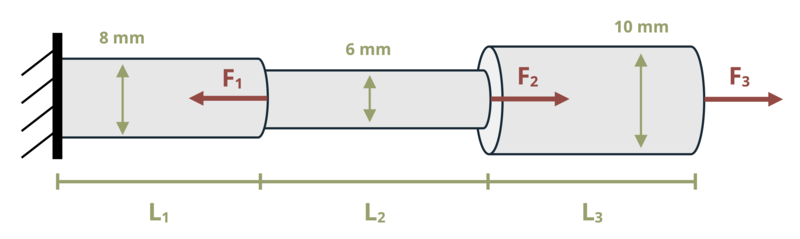
\includegraphics[keepaspectratio]{images/186.png}}
{[}Problem adapted from © Kurt Gramoll CC BY NC-SA 4.0{]}

\begin{Shaded}
\begin{Highlighting}[]
\NormalTok{\#| standalone: true}
\NormalTok{\#| viewerHeight: 600}
\NormalTok{\#| components: [viewer]}

\NormalTok{from shiny import App, render, ui, reactive}
\NormalTok{import random}
\NormalTok{import asyncio}
\NormalTok{import io}
\NormalTok{import math}
\NormalTok{import string}
\NormalTok{from datetime import datetime}
\NormalTok{from pathlib import Path}

\NormalTok{def generate\_random\_letters(length):}
\NormalTok{    \# Generate a random string of letters of specified length}
\NormalTok{    return \textquotesingle{}\textquotesingle{}.join(random.choice(string.ascii\_lowercase) for \_ in range(length))}

\NormalTok{problem\_ID="186"}
\NormalTok{F1=reactive.Value("\_\_")}
\NormalTok{F2=reactive.Value("\_\_")}
\NormalTok{F3=reactive.Value("\_\_")}
\NormalTok{L1=reactive.Value("\_\_")}
\NormalTok{L2=reactive.Value("\_\_")}
\NormalTok{L3=reactive.Value("\_\_")}

\NormalTok{attempts=["Timestamp,Attempt,Answer,Feedback\textbackslash{}n"]}

\NormalTok{app\_ui = ui.page\_fluid(}
\NormalTok{    \#ui.markdown("**Please enter your ID number from your instructor and click to generate your problem**"),}
\NormalTok{    \#ui.input\_text("ID","", placeholder="Enter ID Number Here"),}
\NormalTok{    \#ui.input\_action\_button("generate\_problem", "Generate Problem", class\_="btn{-}primary"),}
\NormalTok{    ui.markdown("**Problem Statement**"),}
\NormalTok{    ui.output\_ui("ui\_problem\_statement"),}
\NormalTok{    ui.input\_text("answer","Your Answer in units of mm", placeholder="Please enter your answer"),}
\NormalTok{    ui.input\_action\_button("submit", "Check Answer", class\_="btn{-}primary"),}
\NormalTok{    \#ui.download\_button("download", "Download File to Submit", class\_="btn{-}success"),}
\NormalTok{)}

\NormalTok{def server(input, output, session):}
\NormalTok{    \# Initialize a counter for attempts}
\NormalTok{    attempt\_counter = reactive.Value(0)}

\NormalTok{    @output}
\NormalTok{    @render.ui}
\NormalTok{    def ui\_problem\_statement():}
\NormalTok{        randomize\_vars()}
\NormalTok{        return[ui.markdown(f"A series of solid circular steel bars are loaded as shown, where F\textless{}sub\textgreater{}1\textless{}/sub\textgreater{} = \{F1()\} N, F\textless{}sub\textgreater{}2\textless{}/sub\textgreater{} = \{F2()\} N, and F\textless{}sub\textgreater{}3\textless{}/sub\textgreater{} = \{F3()\} N. If lengths L\textless{}sub\textgreater{}1\textless{}/sub\textgreater{} = L\textless{}sub\textgreater{}2\textless{}/sub\textgreater{} = \{L1()\} cm and L\textless{}sub\textgreater{}3\textless{}/sub\textgreater{} = \{L3()\} cm, determine the total change in length of the system. Assume E\textless{}sub\textgreater{}steel\textless{}/sub\textgreater{} = 210 GPa.")]}
    
\NormalTok{    \#@reactive.Effect}
\NormalTok{    \#@reactive.event(input.generate\_problem)}
\NormalTok{    def randomize\_vars():}
\NormalTok{        random.seed(101)}
\NormalTok{        F1.set(random.randrange(20, 100, 1))}
\NormalTok{        F2.set(random.randrange(20, 100, 1))}
\NormalTok{        F3.set(random.randrange(20, 100, 1))}
\NormalTok{        L1.set(random.randrange(20, 60, 1))}
\NormalTok{        L2.set(L1())}
\NormalTok{        L3.set(round(L1()*1.25))}
        
\NormalTok{    @reactive.Effect}
\NormalTok{    @reactive.event(input.submit)}
\NormalTok{    def \_():}
\NormalTok{        attempt\_counter.set(attempt\_counter() + 1)  \# Increment the attempt counter on each submission.}
\NormalTok{        R = F2()+F3(){-}F1()}
\NormalTok{        FBC = F1()+R}
\NormalTok{        dAB = R*L1()/100/(210*10**9*0.004**2*math.pi)}
\NormalTok{        dBC = FBC*L2()/100/(210*10**9*0.003**2*math.pi)}
\NormalTok{        dCD = F3()*L3()/100/(210*10**9*0.005**2*math.pi)}
\NormalTok{        instr= abs((dAB+dBC+dCD)*10**3)}
\NormalTok{        if math.isclose(float(input.answer()), instr, rel\_tol=0.01):}
\NormalTok{            check = "*Correct*"}
\NormalTok{            correct\_indicator = "JL"}
\NormalTok{        else:}
\NormalTok{            check = "*Not Correct.*"}
\NormalTok{            correct\_indicator = "JG"}

\NormalTok{        \# Generate random parts for the encoded attempt.}
\NormalTok{        random\_start = generate\_random\_letters(4)}
\NormalTok{        random\_middle = generate\_random\_letters(4)}
\NormalTok{        random\_end = generate\_random\_letters(4)}
\NormalTok{        \#encoded\_attempt = f"\{random\_start\}\{problem\_ID\}{-}\{random\_middle\}\{attempt\_counter()\}\{correct\_indicator\}{-}\{random\_end\}\{input.ID()\}"}

\NormalTok{        \# Store the most recent encoded attempt in a reactive value so it persists across submissions}
\NormalTok{        \#session.encoded\_attempt = reactive.Value(encoded\_attempt)}

\NormalTok{        \# Append the attempt data to the attempts list without the encoded attempt}
\NormalTok{        attempts.append(f"\{datetime.now()\}, \{attempt\_counter()\}, \{input.answer()\}, \{check\}\textbackslash{}n")}

\NormalTok{        \# Show feedback to the user.}
\NormalTok{        feedback = ui.markdown(f"Your answer of \{input.answer()\} is \{check\}.")}
\NormalTok{        m = ui.modal(}
\NormalTok{            feedback,}
\NormalTok{            title="Feedback",}
\NormalTok{            easy\_close=True}
\NormalTok{        )}
\NormalTok{        ui.modal\_show(m)}

\NormalTok{    \#@render.download(filename=lambda: f"Problem\_Log{-}\{problem\_ID\}{-}\{input.ID()\}.csv")}
\NormalTok{    async def download():}
\NormalTok{        \# Start the CSV with the encoded attempt (without label)}
\NormalTok{        final\_encoded = session.encoded\_attempt() if session.encoded\_attempt is not None else "No attempts"}
\NormalTok{        yield f"\{final\_encoded\}\textbackslash{}n\textbackslash{}n"}
        
\NormalTok{        \# Write the header for the remaining CSV data once}
\NormalTok{        yield "Timestamp,Attempt,Answer,Feedback\textbackslash{}n"}
        
\NormalTok{        \# Write the attempts data, ensure that the header from the attempts list is not written again}
\NormalTok{        for attempt in attempts[1:]:  \# Skip the first element which is the header}
\NormalTok{            await asyncio.sleep(0.25)  \# This delay may not be necessary; adjust as needed}
\NormalTok{            yield attempt}

\NormalTok{\# App installation}
\NormalTok{app = App(app\_ui, server)}
\end{Highlighting}
\end{Shaded}

\chapter*{Problem 5.15 - Axial
Deformation}\label{problem-5.15---axial-deformation}
\addcontentsline{toc}{chapter}{Problem 5.15 - Axial Deformation}

\markboth{Problem 5.15 - Axial Deformation}{Problem 5.15 - Axial
Deformation}

\pandocbounded{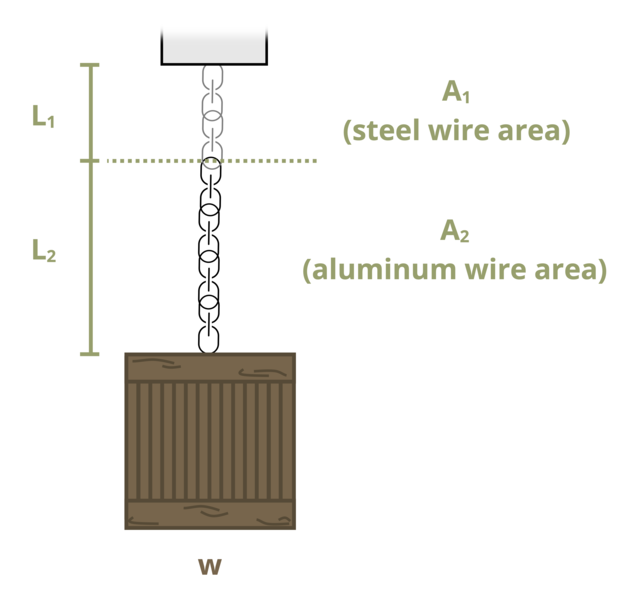
\includegraphics[keepaspectratio]{images/187.png}}
{[}Problem adapted from © Kurt Gramoll CC BY NC-SA 4.0{]}

\begin{Shaded}
\begin{Highlighting}[]
\NormalTok{\#| standalone: true}
\NormalTok{\#| viewerHeight: 600}
\NormalTok{\#| components: [viewer]}

\NormalTok{from shiny import App, render, ui, reactive}
\NormalTok{import random}
\NormalTok{import asyncio}
\NormalTok{import io}
\NormalTok{import math}
\NormalTok{import string}
\NormalTok{from datetime import datetime}
\NormalTok{from pathlib import Path}

\NormalTok{def generate\_random\_letters(length):}
\NormalTok{    \# Generate a random string of letters of specified length}
\NormalTok{    return \textquotesingle{}\textquotesingle{}.join(random.choice(string.ascii\_lowercase) for \_ in range(length)) }

\NormalTok{problem\_ID="187"}
\NormalTok{W=reactive.Value("\_\_")}
\NormalTok{L1=reactive.Value("\_\_")}
\NormalTok{L2=reactive.Value("\_\_")}
\NormalTok{A1=reactive.Value("\_\_")}
\NormalTok{A2=reactive.Value("\_\_")}
\NormalTok{Esteel = 29000}
\NormalTok{Ealuminum = 10000}

\NormalTok{attempts=["Timestamp,Attempt,Answer,Feedback\textbackslash{}n"]}

\NormalTok{app\_ui = ui.page\_fluid(}
\NormalTok{    \#ui.markdown("**Please enter your ID number from your instructor and click to generate your problem**"),}
\NormalTok{    \#ui.input\_text("ID","", placeholder="Enter ID Number Here"),}
\NormalTok{    \#ui.input\_action\_button("generate\_problem", "Generate Problem", class\_="btn{-}primary"),}
\NormalTok{    ui.markdown("**Problem Statement**"),}
\NormalTok{    ui.output\_ui("ui\_problem\_statement"),}
\NormalTok{    ui.input\_text("answer","Your Answer in units of inches", placeholder="Please enter your answer"),}
\NormalTok{    ui.input\_action\_button("submit", "Check Answer", class\_="btn{-}primary"),}
\NormalTok{    \#ui.download\_button("download", "Download File to Submit", class\_="btn{-}success"),}
\NormalTok{)}

\NormalTok{def server(input, output, session):}
\NormalTok{    \# Initialize a counter for attempts}
\NormalTok{    attempt\_counter = reactive.Value(0)}

\NormalTok{    @output}
\NormalTok{    @render.ui}
\NormalTok{    def ui\_problem\_statement():}
\NormalTok{        randomize\_vars()}
\NormalTok{        return[ui.markdown(f"A crate weight W = \{W()\} lb is attached to a cable constructed from steel of length L\textless{}sub\textgreater{}1\textless{}/sub\textgreater{} = \{L1()\} in. and Area A\textless{}sub\textgreater{}1\textless{}/sub\textgreater{} = \{A1()\} in.\textless{}sup\textgreater{}2\textless{}/sup\textgreater{} and aluminum of length L\textless{}sub\textgreater{}2\textless{}/sub\textgreater{} = \{L2()\} in. and area A\textless{}sub\textgreater{}2\textless{}/sub\textgreater{} = \{A2()\} in.\textless{}sup\textgreater{}2\textless{}/sup\textgreater{}. What is the total deflection of the crate after it is attached to the wire? Assume E\textless{}sub\textgreater{}steel\textless{}/sub\textgreater{} = \{Esteel\} ksi and E\textless{}sub\textgreater{}aluminum\textless{}/sub\textgreater{} = \{Ealuminum\} ksi. Neglect the weight of the wires.")]}
    
\NormalTok{    \#@reactive.Effect}
\NormalTok{    \#@reactive.event(input.generate\_problem)}
\NormalTok{    def randomize\_vars():}
\NormalTok{        random.seed(101)}
\NormalTok{        W.set(random.randrange(50, 250, 1))}
\NormalTok{        L1.set(random.randrange(10, 30, 1))}
\NormalTok{        L2.set(round(L1()*2, 2))}
\NormalTok{        A1.set(random.randrange(1, 5, 1)/100)}
\NormalTok{        A2.set(random.randrange(1, 5, 1)/100)}
        
\NormalTok{    @reactive.Effect}
\NormalTok{    @reactive.event(input.submit)}
\NormalTok{    def \_():}
\NormalTok{        attempt\_counter.set(attempt\_counter() + 1)  \# Increment the attempt counter on each submission.}
        
\NormalTok{        instr=(W()*L1()/(A1()*Esteel*1000) + (W()*L2()/(A2()*Ealuminum*1000)))}
\NormalTok{        if math.isclose(float(input.answer()), instr, rel\_tol=0.01):}
\NormalTok{            check = "*Correct*"}
\NormalTok{            correct\_indicator = "JL"}
\NormalTok{        else:}
\NormalTok{            check = "*Not Correct.*"}
\NormalTok{            correct\_indicator = "JG"}

\NormalTok{        \# Generate random parts for the encoded attempt.}
\NormalTok{        random\_start = generate\_random\_letters(4)}
\NormalTok{        random\_middle = generate\_random\_letters(4)}
\NormalTok{        random\_end = generate\_random\_letters(4)}
\NormalTok{        \#encoded\_attempt = f"\{random\_start\}\{problem\_ID\}{-}\{random\_middle\}\{attempt\_counter()\}\{correct\_indicator\}{-}\{random\_end\}\{input.ID()\}"}

\NormalTok{        \# Store the most recent encoded attempt in a reactive value so it persists across submissions}
\NormalTok{        \#session.encoded\_attempt = reactive.Value(encoded\_attempt)}

\NormalTok{        \# Append the attempt data to the attempts list without the encoded attempt}
\NormalTok{        attempts.append(f"\{datetime.now()\}, \{attempt\_counter()\}, \{input.answer()\}, \{check\}\textbackslash{}n")}

\NormalTok{        \# Show feedback to the user.}
\NormalTok{        feedback = ui.markdown(f"Your answer of \{input.answer()\} is \{check\}.")}
\NormalTok{        m = ui.modal(}
\NormalTok{            feedback,}
\NormalTok{            title="Feedback",}
\NormalTok{            easy\_close=True}
\NormalTok{        )}
\NormalTok{        ui.modal\_show(m)}

\NormalTok{    \#@render.download(filename=lambda: f"Problem\_Log{-}\{problem\_ID\}{-}\{input.ID()\}.csv")}
\NormalTok{    async def download():}
\NormalTok{        \# Start the CSV with the encoded attempt (without label)}
\NormalTok{        final\_encoded = session.encoded\_attempt() if session.encoded\_attempt is not None else "No attempts"}
\NormalTok{        yield f"\{final\_encoded\}\textbackslash{}n\textbackslash{}n"}
        
\NormalTok{        \# Write the header for the remaining CSV data once}
\NormalTok{        yield "Timestamp,Attempt,Answer,Feedback\textbackslash{}n"}
        
\NormalTok{        \# Write the attempts data, ensure that the header from the attempts list is not written again}
\NormalTok{        for attempt in attempts[1:]:  \# Skip the first element which is the header}
\NormalTok{            await asyncio.sleep(0.25)  \# This delay may not be necessary; adjust as needed}
\NormalTok{            yield attempt}

\NormalTok{\# App installation}
\NormalTok{app = App(app\_ui, server)}
\end{Highlighting}
\end{Shaded}

\chapter*{Problem 5.16 - Axial
Deformation}\label{problem-5.16---axial-deformation}
\addcontentsline{toc}{chapter}{Problem 5.16 - Axial Deformation}

\markboth{Problem 5.16 - Axial Deformation}{Problem 5.16 - Axial
Deformation}

\pandocbounded{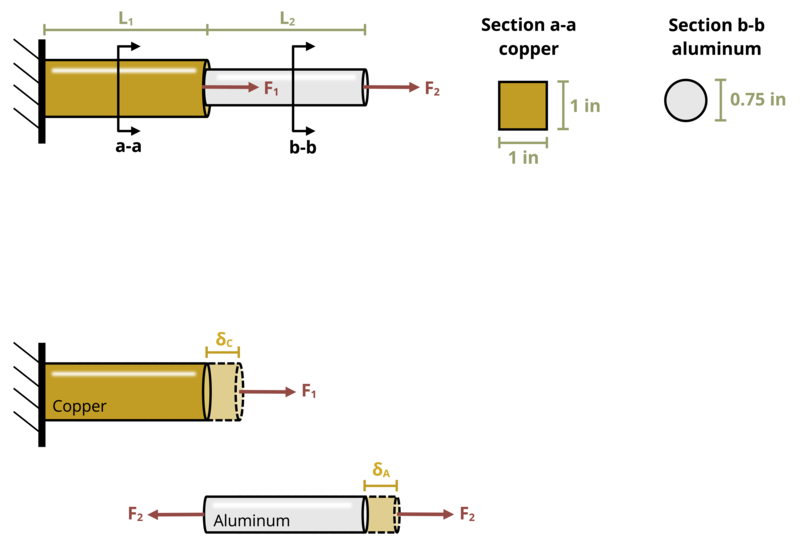
\includegraphics[keepaspectratio]{images/190.png}}
{[}Problem adapted from © Kurt Gramoll CC BY NC-SA 4.0{]}

\begin{Shaded}
\begin{Highlighting}[]
\NormalTok{\#| standalone: true}
\NormalTok{\#| viewerHeight: 600}
\NormalTok{\#| components: [viewer]}

\NormalTok{from shiny import App, render, ui, reactive}
\NormalTok{import random}
\NormalTok{import asyncio}
\NormalTok{import io}
\NormalTok{import math}
\NormalTok{import string}
\NormalTok{from datetime import datetime}
\NormalTok{from pathlib import Path}

\NormalTok{def generate\_random\_letters(length):}
\NormalTok{    \# Generate a random string of letters of specified length}
\NormalTok{    return \textquotesingle{}\textquotesingle{}.join(random.choice(string.ascii\_lowercase) for \_ in range(length))  }
\NormalTok{problem\_ID="190"}
\NormalTok{F1=reactive.Value("\_\_")}
\NormalTok{F2=reactive.Value("\_\_")}
\NormalTok{L1=reactive.Value("\_\_")}
\NormalTok{L2=reactive.Value("\_\_")}
  
\NormalTok{attempts=["Timestamp,Attempt,Answer,Feedback\textbackslash{}n"]}

\NormalTok{app\_ui = ui.page\_fluid(}
\NormalTok{    \#ui.markdown("**Please enter your ID number from your instructor and click to generate your problem**"),}
\NormalTok{    \#ui.input\_text("ID","", placeholder="Enter ID Number Here"),}
\NormalTok{    \#ui.input\_action\_button("generate\_problem", "Generate Problem", class\_="btn{-}primary"),}
\NormalTok{    ui.markdown("**Problem Statement**"),}
\NormalTok{    ui.output\_ui("ui\_problem\_statement"),}
\NormalTok{    ui.input\_text("answer","Your Answer in units of in", placeholder="Please enter your answer"),}
\NormalTok{    ui.input\_action\_button("submit", "Check Answer", class\_="btn{-}primary"),}
\NormalTok{    \#ui.download\_button("download", "Download File to Submit", class\_="btn{-}success"),}
\NormalTok{)}

\NormalTok{def server(input, output, session):}
\NormalTok{    \# Initialize a counter for attempts}
\NormalTok{    attempt\_counter = reactive.Value(0)}

\NormalTok{    @output}
\NormalTok{    @render.ui}
\NormalTok{    def ui\_problem\_statement():}
\NormalTok{        randomize\_vars()}
\NormalTok{        return[ui.markdown(f"A solid square rod and round bar are pulled in series as shown. If load F\textless{}sub\textgreater{}1\textless{}/sub\textgreater{} =  \{F1()\} kip, load F\textless{}sub\textgreater{}2\textless{}/sub\textgreater{} = \{F2()\} kip, length L\textless{}sub\textgreater{}1\textless{}/sub\textgreater{} = \{L1()\} in., and length L\textless{}sub\textgreater{}2\textless{}/sub\textgreater{} = \{L2()\} in., determine the total displacement of the right tip of the structure. Assume E\textless{}sub\textgreater{}copper\textless{}/sub\textgreater{} = 16x10\textless{}sup\textgreater{}6\textless{}/sup\textgreater{} psi and E\textless{}sub\textgreater{}aluminum\textless{}/sub\textgreater{} = 10x10\textless{}sup\textgreater{}6\textless{}/sup\textgreater{} psi.")]}
    
\NormalTok{    \#@reactive.Effect}
\NormalTok{    \#@reactive.event(input.generate\_problem)}
\NormalTok{    def randomize\_vars():}
\NormalTok{        random.seed(101)}
\NormalTok{        F1.set(random.randrange(10,30,1))}
\NormalTok{        F2.set(random.randrange(10,30,1))}
\NormalTok{        L1.set(random.randrange(6,25,1))}
\NormalTok{        L2.set(round(L1()*1.4,1))}
        
\NormalTok{    @reactive.Effect}
\NormalTok{    @reactive.event(input.submit)}
\NormalTok{    def \_():}
\NormalTok{        attempt\_counter.set(attempt\_counter() + 1)  \# Increment the attempt counter on each submission.}
\NormalTok{        Pc = (F1()+F2())*1000}
\NormalTok{        Ec = 16*10**6}
\NormalTok{        Ac = 1}
\NormalTok{        Pa = F2()*1000}
\NormalTok{        Ea = 10*10**6}
\NormalTok{        Aa = 0.375**2*math.pi}
\NormalTok{        instr = Pc*L1()/(Ec*Ac)+Pa*L2()/(Ea*Aa)}
        
\NormalTok{        if math.isclose(float(input.answer()), instr, rel\_tol=0.01):}
\NormalTok{            check = "*Correct*"}
\NormalTok{            correct\_indicator = "JL"}
\NormalTok{        else:}
\NormalTok{            check = "*Not Correct.*"}
\NormalTok{            correct\_indicator = "JG"}

\NormalTok{        \# Generate random parts for the encoded attempt.}
\NormalTok{        random\_start = generate\_random\_letters(4)}
\NormalTok{        random\_middle = generate\_random\_letters(4)}
\NormalTok{        random\_end = generate\_random\_letters(4)}
\NormalTok{        \#encoded\_attempt = f"\{random\_start\}\{problem\_ID\}{-}\{random\_middle\}\{attempt\_counter()\}\{correct\_indicator\}{-}\{random\_end\}\{input.ID()\}"}

\NormalTok{        \# Store the most recent encoded attempt in a reactive value so it persists across submissions}
\NormalTok{        \#session.encoded\_attempt = reactive.Value(encoded\_attempt)}

\NormalTok{        \# Append the attempt data to the attempts list without the encoded attempt}
\NormalTok{        attempts.append(f"\{datetime.now()\}, \{attempt\_counter()\}, \{input.answer()\}, \{check\}\textbackslash{}n")}

\NormalTok{        \# Show feedback to the user.}
\NormalTok{        feedback = ui.markdown(f"Your answer of \{input.answer()\} is \{check\}.")}
\NormalTok{        m = ui.modal(}
\NormalTok{            feedback,}
\NormalTok{            title="Feedback",}
\NormalTok{            easy\_close=True}
\NormalTok{        )}
\NormalTok{        ui.modal\_show(m)}

\NormalTok{    \#@render.download(filename=lambda: f"Problem\_Log{-}\{problem\_ID\}{-}\{input.ID()\}.csv")}
\NormalTok{    async def download():}
\NormalTok{        \# Start the CSV with the encoded attempt (without label)}
\NormalTok{        final\_encoded = session.encoded\_attempt() if session.encoded\_attempt is not None else "No attempts"}
\NormalTok{        yield f"\{final\_encoded\}\textbackslash{}n\textbackslash{}n"}
        
\NormalTok{        \# Write the header for the remaining CSV data once}
\NormalTok{        yield "Timestamp,Attempt,Answer,Feedback\textbackslash{}n"}
        
\NormalTok{        \# Write the attempts data, ensure that the header from the attempts list is not written again}
\NormalTok{        for attempt in attempts[1:]:  \# Skip the first element which is the header}
\NormalTok{            await asyncio.sleep(0.25)  \# This delay may not be necessary; adjust as needed}
\NormalTok{            yield attempt}

\NormalTok{\# App installation}
\NormalTok{app = App(app\_ui, server)}
\end{Highlighting}
\end{Shaded}

\chapter*{Problem 5.17 - Axial
Deformation}\label{problem-5.17---axial-deformation}
\addcontentsline{toc}{chapter}{Problem 5.17 - Axial Deformation}

\markboth{Problem 5.17 - Axial Deformation}{Problem 5.17 - Axial
Deformation}

\pandocbounded{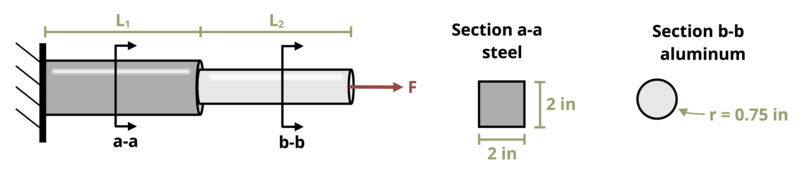
\includegraphics[keepaspectratio]{images/195.png}}
{[}Problem adapted from © Kurt Gramoll CC BY NC-SA 4.0{]}

\begin{Shaded}
\begin{Highlighting}[]
\NormalTok{\#| standalone: true}
\NormalTok{\#| viewerHeight: 600}
\NormalTok{\#| components: [viewer]}

\NormalTok{from shiny import App, render, ui, reactive}
\NormalTok{import random}
\NormalTok{import asyncio}
\NormalTok{import io}
\NormalTok{import math}
\NormalTok{import string}
\NormalTok{from datetime import datetime}
\NormalTok{from pathlib import Path}

\NormalTok{def generate\_random\_letters(length):}
\NormalTok{    \# Generate a random string of letters of specified length}
\NormalTok{    return \textquotesingle{}\textquotesingle{}.join(random.choice(string.ascii\_lowercase) for \_ in range(length))  }

\NormalTok{problem\_ID="190"}
\NormalTok{F1=reactive.Value("\_\_")}
\NormalTok{F2=reactive.Value("\_\_")}
\NormalTok{L1=reactive.Value("\_\_")}
\NormalTok{L2=reactive.Value("\_\_")}
  
\NormalTok{attempts=["Timestamp,Attempt,Answer,Feedback\textbackslash{}n"]}

\NormalTok{app\_ui = ui.page\_fluid(}
\NormalTok{    \#ui.markdown("**Please enter your ID number from your instructor and click to generate your problem**"),}
\NormalTok{    \#ui.input\_text("ID","", placeholder="Enter ID Number Here"),}
\NormalTok{    \#ui.input\_action\_button("generate\_problem", "Generate Problem", class\_="btn{-}primary"),}
\NormalTok{    ui.markdown("**Problem Statement**"),}
\NormalTok{    ui.output\_ui("ui\_problem\_statement"),}
\NormalTok{    ui.input\_text("answer","Your Answer in units of in", placeholder="Please enter your answer"),}
\NormalTok{    ui.input\_action\_button("submit", "Check Answer", class\_="btn{-}primary"),}
\NormalTok{    \#ui.download\_button("download", "Download File to Submit", class\_="btn{-}success"),}
\NormalTok{)}

\NormalTok{def server(input, output, session):}
\NormalTok{    \# Initialize a counter for attempts}
\NormalTok{    attempt\_counter = reactive.Value(0)}

\NormalTok{    @output}
\NormalTok{    @render.ui}
\NormalTok{    def ui\_problem\_statement():}
\NormalTok{        randomize\_vars()}
\NormalTok{        return[ui.markdown(f"A solid square rod and round bar are pulled in series as shown. If load F =  \{F1()\} kip, length L\textless{}sub\textgreater{}1\textless{}/sub\textgreater{} = \{L1()\} in., and length L\textless{}sub\textgreater{}2\textless{}/sub\textgreater{} = \{L2()\} in., determine the total displacement of the right tip of the structure. Assume E\textless{}sub\textgreater{}steel\textless{}/sub\textgreater{} = 29x10\textless{}sup\textgreater{}6\textless{}/sup\textgreater{} psi and E\textless{}sub\textgreater{}aluminum\textless{}/sub\textgreater{} = 10x10\textless{}sup\textgreater{}6\textless{}/sup\textgreater{} psi.")]}
    
\NormalTok{    \#@reactive.Effect}
\NormalTok{    \#@reactive.event(input.generate\_problem)}
\NormalTok{    def randomize\_vars():}
\NormalTok{        random.seed(101)}
\NormalTok{        F1.set(random.randrange(150,400,10))}
\NormalTok{        L1.set(random.randrange(6,25,1))}
\NormalTok{        L2.set(round(L1()*1.4,1))}
        
\NormalTok{    @reactive.Effect}
\NormalTok{    @reactive.event(input.submit)}
\NormalTok{    def \_():}
\NormalTok{        attempt\_counter.set(attempt\_counter() + 1)  \# Increment the attempt counter on each submission.}
\NormalTok{        Ps = F1()*1000}
\NormalTok{        Es = 29*10**6}
\NormalTok{        As = 4}
\NormalTok{        Pa = F1()*1000}
\NormalTok{        Ea = 10*10**6}
\NormalTok{        Aa = 0.75**2*math.pi}
\NormalTok{        instr = Ps*L1()/(Es*As)+Pa*L2()/(Ea*Aa)}
        
\NormalTok{        if math.isclose(float(input.answer()), instr, rel\_tol=0.01):}
\NormalTok{            check = "*Correct*"}
\NormalTok{            correct\_indicator = "JL"}
\NormalTok{        else:}
\NormalTok{            check = "*Not Correct.*"}
\NormalTok{            correct\_indicator = "JG"}

\NormalTok{        \# Generate random parts for the encoded attempt.}
\NormalTok{        random\_start = generate\_random\_letters(4)}
\NormalTok{        random\_middle = generate\_random\_letters(4)}
\NormalTok{        random\_end = generate\_random\_letters(4)}
\NormalTok{        \#encoded\_attempt = f"\{random\_start\}\{problem\_ID\}{-}\{random\_middle\}\{attempt\_counter()\}\{correct\_indicator\}{-}\{random\_end\}\{input.ID()\}"}

\NormalTok{        \# Store the most recent encoded attempt in a reactive value so it persists across submissions}
\NormalTok{        \#session.encoded\_attempt = reactive.Value(encoded\_attempt)}

\NormalTok{        \# Append the attempt data to the attempts list without the encoded attempt}
\NormalTok{        attempts.append(f"\{datetime.now()\}, \{attempt\_counter()\}, \{input.answer()\}, \{check\}\textbackslash{}n")}

\NormalTok{        \# Show feedback to the user.}
\NormalTok{        feedback = ui.markdown(f"Your answer of \{input.answer()\} is \{check\}.")}
\NormalTok{        m = ui.modal(}
\NormalTok{            feedback,}
\NormalTok{            title="Feedback",}
\NormalTok{            easy\_close=True}
\NormalTok{        )}
\NormalTok{        ui.modal\_show(m)}

\NormalTok{    \#@render.download(filename=lambda: f"Problem\_Log{-}\{problem\_ID\}{-}\{input.ID()\}.csv")}
\NormalTok{    async def download():}
\NormalTok{        \# Start the CSV with the encoded attempt (without label)}
\NormalTok{        final\_encoded = session.encoded\_attempt() if session.encoded\_attempt is not None else "No attempts"}
\NormalTok{        yield f"\{final\_encoded\}\textbackslash{}n\textbackslash{}n"}
        
\NormalTok{        \# Write the header for the remaining CSV data once}
\NormalTok{        yield "Timestamp,Attempt,Answer,Feedback\textbackslash{}n"}
        
\NormalTok{        \# Write the attempts data, ensure that the header from the attempts list is not written again}
\NormalTok{        for attempt in attempts[1:]:  \# Skip the first element which is the header}
\NormalTok{            await asyncio.sleep(0.25)  \# This delay may not be necessary; adjust as needed}
\NormalTok{            yield attempt}

\NormalTok{\# App installation}
\NormalTok{app = App(app\_ui, server)}
\end{Highlighting}
\end{Shaded}

\chapter*{Problem 5.18 - Axial
Deformation}\label{problem-5.18---axial-deformation}
\addcontentsline{toc}{chapter}{Problem 5.18 - Axial Deformation}

\markboth{Problem 5.18 - Axial Deformation}{Problem 5.18 - Axial
Deformation}

\pandocbounded{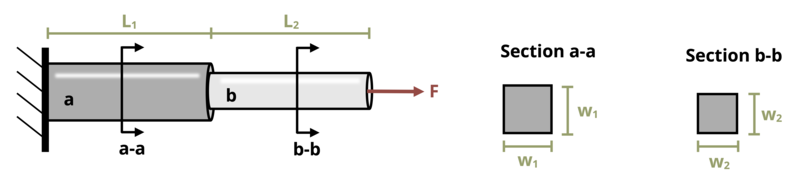
\includegraphics[keepaspectratio]{images/197.png}}
{[}Problem adapted from © Kurt Gramoll CC BY NC-SA 4.0{]}

\begin{Shaded}
\begin{Highlighting}[]
\NormalTok{\#| standalone: true}
\NormalTok{\#| viewerHeight: 600}
\NormalTok{\#| components: [viewer]}

\NormalTok{from shiny import App, render, ui, reactive}
\NormalTok{import random}
\NormalTok{import asyncio}
\NormalTok{import io}
\NormalTok{import math}
\NormalTok{import string}
\NormalTok{from datetime import datetime}
\NormalTok{from pathlib import Path}

\NormalTok{def generate\_random\_letters(length):}
\NormalTok{    \# Generate a random string of letters of specified length}
\NormalTok{    return \textquotesingle{}\textquotesingle{}.join(random.choice(string.ascii\_lowercase) for \_ in range(length))  }

\NormalTok{problem\_ID="197"}
\NormalTok{w2=reactive.Value("\_\_")}
\NormalTok{w1=reactive.Value("\_\_")}
\NormalTok{F=reactive.Value("\_\_")}
  
\NormalTok{attempts=["Timestamp,Attempt,Answer,Feedback\textbackslash{}n"]}

\NormalTok{app\_ui = ui.page\_fluid(}
\NormalTok{    \#ui.markdown("**Please enter your ID number from your instructor and click to generate your problem**"),}
\NormalTok{    \#ui.input\_text("ID","", placeholder="Enter ID Number Here"),}
\NormalTok{    \#ui.input\_action\_button("generate\_problem", "Generate Problem", class\_="btn{-}primary"),}
\NormalTok{    ui.markdown("**Problem Statement**"),}
\NormalTok{    ui.output\_ui("ui\_problem\_statement"),}
\NormalTok{    ui.input\_text("answer","Your Answer in terms of 10\^{}{-}6", placeholder="Please enter your answer"),}
\NormalTok{    ui.input\_action\_button("submit", "Check Answer", class\_="btn{-}primary"),}
\NormalTok{    \#ui.download\_button("download", "Download File to Submit", class\_="btn{-}success"),}
\NormalTok{)}

\NormalTok{def server(input, output, session):}
\NormalTok{    \# Initialize a counter for attempts}
\NormalTok{    attempt\_counter = reactive.Value(0)}

\NormalTok{    @output}
\NormalTok{    @render.ui}
\NormalTok{    def ui\_problem\_statement():}
\NormalTok{        randomize\_vars()}
\NormalTok{        return[ui.markdown(f"Two solid square cross{-}sections with dimensions w\textless{}sub\textgreater{}1\textless{}/sub\textgreater{} = \{w1()\} mm and w\textless{}sub\textgreater{}2\textless{}/sub\textgreater{} = \{w2()\} mm are pulled in series by load F = \{F()\} kN. Determine the normal strain in rod b in the direction of the load. Assume E = 200 GPa.")]}
    
\NormalTok{    \#@reactive.Effect}
\NormalTok{    \#@reactive.event(input.generate\_problem)}
\NormalTok{    def randomize\_vars():}
\NormalTok{        random.seed(101)}
\NormalTok{        w2.set(random.randrange(25,80,1))}
\NormalTok{        w1.set(round(w2()*1.25))}
\NormalTok{        F.set(random.randrange(200,800,10))}

\NormalTok{    @reactive.Effect}
\NormalTok{    @reactive.event(input.submit)}
\NormalTok{    def \_():}
\NormalTok{        attempt\_counter.set(attempt\_counter() + 1)  \# Increment the attempt counter on each submission.}
\NormalTok{        delb = F()*0.6/(200*10**6*(w2()/1000)**2)}
\NormalTok{        instr = delb/0.6*10**6}
        
\NormalTok{        if math.isclose(float(input.answer()), instr, rel\_tol=0.01):}
\NormalTok{            check = "*Correct*"}
\NormalTok{            correct\_indicator = "JL"}
\NormalTok{        else:}
\NormalTok{            check = "*Not Correct.*"}
\NormalTok{            correct\_indicator = "JG"}

\NormalTok{        \# Generate random parts for the encoded attempt.}
\NormalTok{        random\_start = generate\_random\_letters(4)}
\NormalTok{        random\_middle = generate\_random\_letters(4)}
\NormalTok{        random\_end = generate\_random\_letters(4)}
\NormalTok{        \#encoded\_attempt = f"\{random\_start\}\{problem\_ID\}{-}\{random\_middle\}\{attempt\_counter()\}\{correct\_indicator\}{-}\{random\_end\}\{input.ID()\}"}

\NormalTok{        \# Store the most recent encoded attempt in a reactive value so it persists across submissions}
\NormalTok{        \#session.encoded\_attempt = reactive.Value(encoded\_attempt)}

\NormalTok{        \# Append the attempt data to the attempts list without the encoded attempt}
\NormalTok{        attempts.append(f"\{datetime.now()\}, \{attempt\_counter()\}, \{input.answer()\}, \{check\}\textbackslash{}n")}

\NormalTok{        \# Show feedback to the user.}
\NormalTok{        feedback = ui.markdown(f"Your answer of \{input.answer()\} is \{check\}.")}
\NormalTok{        m = ui.modal(}
\NormalTok{            feedback,}
\NormalTok{            title="Feedback",}
\NormalTok{            easy\_close=True}
\NormalTok{        )}
\NormalTok{        ui.modal\_show(m)}

\NormalTok{    \#@render.download(filename=lambda: f"Problem\_Log{-}\{problem\_ID\}{-}\{input.ID()\}.csv")}
\NormalTok{    async def download():}
\NormalTok{        \# Start the CSV with the encoded attempt (without label)}
\NormalTok{        final\_encoded = session.encoded\_attempt() if session.encoded\_attempt is not None else "No attempts"}
\NormalTok{        yield f"\{final\_encoded\}\textbackslash{}n\textbackslash{}n"}
        
\NormalTok{        \# Write the header for the remaining CSV data once}
\NormalTok{        yield "Timestamp,Attempt,Answer,Feedback\textbackslash{}n"}
        
\NormalTok{        \# Write the attempts data, ensure that the header from the attempts list is not written again}
\NormalTok{        for attempt in attempts[1:]:  \# Skip the first element which is the header}
\NormalTok{            await asyncio.sleep(0.25)  \# This delay may not be necessary; adjust as needed}
\NormalTok{            yield attempt}

\NormalTok{\# App installation}
\NormalTok{app = App(app\_ui, server)}
\end{Highlighting}
\end{Shaded}

\chapter*{Problem 5.19 - Axial
Deformation}\label{problem-5.19---axial-deformation}
\addcontentsline{toc}{chapter}{Problem 5.19 - Axial Deformation}

\markboth{Problem 5.19 - Axial Deformation}{Problem 5.19 - Axial
Deformation}

\pandocbounded{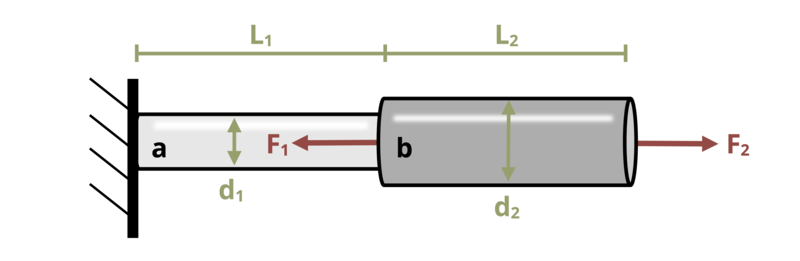
\includegraphics[keepaspectratio]{images/198.png}}
{[}Problem adapted from © Kurt Gramoll CC BY NC-SA 4.0{]}

\begin{Shaded}
\begin{Highlighting}[]
\NormalTok{\#| standalone: true}
\NormalTok{\#| viewerHeight: 600}
\NormalTok{\#| components: [viewer]}

\NormalTok{from shiny import App, render, ui, reactive}
\NormalTok{import random}
\NormalTok{import asyncio}
\NormalTok{import io}
\NormalTok{import math}
\NormalTok{import string}
\NormalTok{from datetime import datetime}
\NormalTok{from pathlib import Path}

\NormalTok{def generate\_random\_letters(length):}
\NormalTok{    \# Generate a random string of letters of specified length}
\NormalTok{    return \textquotesingle{}\textquotesingle{}.join(random.choice(string.ascii\_lowercase) for \_ in range(length))  }

\NormalTok{problem\_ID="198"}
\NormalTok{F1=reactive.Value("\_\_")}
\NormalTok{F2=reactive.Value("\_\_")}
\NormalTok{L2=reactive.Value("\_\_")}
\NormalTok{L1=reactive.Value("\_\_")}
  
\NormalTok{attempts=["Timestamp,Attempt,Answer,Feedback\textbackslash{}n"]}

\NormalTok{app\_ui = ui.page\_fluid(}
\NormalTok{    \#ui.markdown("**Please enter your ID number from your instructor and click to generate your problem**"),}
\NormalTok{    \#ui.input\_text("ID","", placeholder="Enter ID Number Here"),}
\NormalTok{    \#ui.input\_action\_button("generate\_problem", "Generate Problem", class\_="btn{-}primary"),}
\NormalTok{    ui.markdown("**Problem Statement**"),}
\NormalTok{    ui.output\_ui("ui\_problem\_statement"),}
\NormalTok{    ui.input\_text("answer","Your Answer in units of mm", placeholder="Please enter your answer"),}
\NormalTok{    ui.input\_action\_button("submit", "Check Answer", class\_="btn{-}primary"),}
\NormalTok{    \#ui.download\_button("download", "Download File to Submit", class\_="btn{-}success"),}
\NormalTok{)}

\NormalTok{def server(input, output, session):}
\NormalTok{    \# Initialize a counter for attempts}
\NormalTok{    attempt\_counter = reactive.Value(0)}

\NormalTok{    @output}
\NormalTok{    @render.ui}
\NormalTok{    def ui\_problem\_statement():}
\NormalTok{        randomize\_vars()}
\NormalTok{        return[ui.markdown(f"Two circular rods are attached together and loaded with forces F\textless{}sub\textgreater{}1\textless{}/sub\textgreater{} = \{F1()\} kN and F\textless{}sub\textgreater{}2\textless{}/sub\textgreater{} = \{F2()\} kN as shown. If length L\textless{}sub\textgreater{}1\textless{}/sub\textgreater{} = \{L1()\} mm and length L\textless{}sub\textgreater{}2\textless{}/sub\textgreater{} = \{L2()\} mm, determine the total deflection of the right end. Assume E = 69 GPa for both rods.")]}
    
\NormalTok{    \#@reactive.Effect}
\NormalTok{    \#@reactive.event(input.generate\_problem)}
\NormalTok{    def randomize\_vars():}
\NormalTok{        random.seed(101)}
\NormalTok{        F1.set(random.randrange(100,200,1)/10)}
\NormalTok{        F2.set(round(F1(),1)+round(random.randrange(50,150,1)/10))}
\NormalTok{        L2.set(random.randrange(200,400,10))}
\NormalTok{        L1.set(L2()*1.2)}

\NormalTok{    @reactive.Effect}
\NormalTok{    @reactive.event(input.submit)}
\NormalTok{    def \_():}
\NormalTok{        attempt\_counter.set(attempt\_counter() + 1)  \# Increment the attempt counter on each submission.}
\NormalTok{        Pa = F2(){-}F1()}
\NormalTok{        Pb = F2()}
\NormalTok{        E = 69*10**9}
\NormalTok{        delA = Pa*L1()/(E*0.0125**2*math.pi)}
\NormalTok{        delB = Pb*L2()/(E*0.015**2*math.pi)}
\NormalTok{        instr = (delA+delB)*10**3}
        
\NormalTok{        if math.isclose(float(input.answer()), instr, rel\_tol=0.01):}
\NormalTok{            check = "*Correct*"}
\NormalTok{            correct\_indicator = "JL"}
\NormalTok{        else:}
\NormalTok{            check = "*Not Correct.*"}
\NormalTok{            correct\_indicator = "JG"}

\NormalTok{        \# Generate random parts for the encoded attempt.}
\NormalTok{        random\_start = generate\_random\_letters(4)}
\NormalTok{        random\_middle = generate\_random\_letters(4)}
\NormalTok{        random\_end = generate\_random\_letters(4)}
\NormalTok{        \#encoded\_attempt = f"\{random\_start\}\{problem\_ID\}{-}\{random\_middle\}\{attempt\_counter()\}\{correct\_indicator\}{-}\{random\_end\}\{input.ID()\}"}

\NormalTok{        \# Store the most recent encoded attempt in a reactive value so it persists across submissions}
\NormalTok{        \#session.encoded\_attempt = reactive.Value(encoded\_attempt)}

\NormalTok{        \# Append the attempt data to the attempts list without the encoded attempt}
\NormalTok{        attempts.append(f"\{datetime.now()\}, \{attempt\_counter()\}, \{input.answer()\}, \{check\}\textbackslash{}n")}

\NormalTok{        \# Show feedback to the user.}
\NormalTok{        feedback = ui.markdown(f"Your answer of \{input.answer()\} is \{check\}.")}
\NormalTok{        m = ui.modal(}
\NormalTok{            feedback,}
\NormalTok{            title="Feedback",}
\NormalTok{            easy\_close=True}
\NormalTok{        )}
\NormalTok{        ui.modal\_show(m)}

\NormalTok{    \#@render.download(filename=lambda: f"Problem\_Log{-}\{problem\_ID\}{-}\{input.ID()\}.csv")}
\NormalTok{    async def download():}
\NormalTok{        \# Start the CSV with the encoded attempt (without label)}
\NormalTok{        final\_encoded = session.encoded\_attempt() if session.encoded\_attempt is not None else "No attempts"}
\NormalTok{        yield f"\{final\_encoded\}\textbackslash{}n\textbackslash{}n"}
        
\NormalTok{        \# Write the header for the remaining CSV data once}
\NormalTok{        yield "Timestamp,Attempt,Answer,Feedback\textbackslash{}n"}
        
\NormalTok{        \# Write the attempts data, ensure that the header from the attempts list is not written again}
\NormalTok{        for attempt in attempts[1:]:  \# Skip the first element which is the header}
\NormalTok{            await asyncio.sleep(0.25)  \# This delay may not be necessary; adjust as needed}
\NormalTok{            yield attempt}

\NormalTok{\# App installation}
\NormalTok{app = App(app\_ui, server)}
\end{Highlighting}
\end{Shaded}

\chapter*{Problem 5.20 - Axial
Deformation}\label{problem-5.20---axial-deformation}
\addcontentsline{toc}{chapter}{Problem 5.20 - Axial Deformation}

\markboth{Problem 5.20 - Axial Deformation}{Problem 5.20 - Axial
Deformation}

\pandocbounded{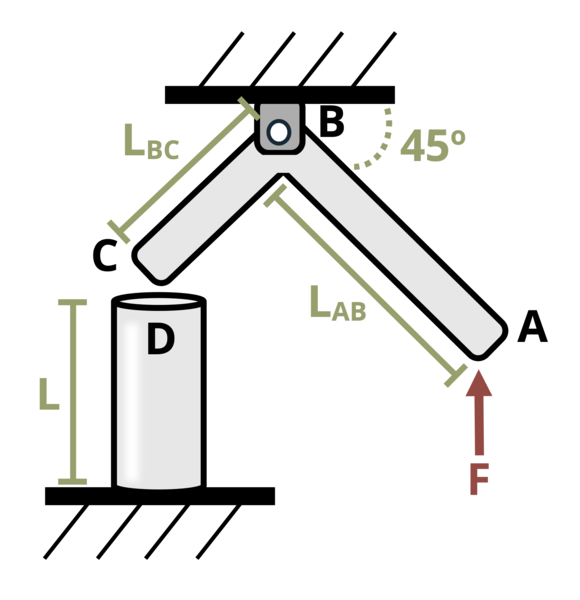
\includegraphics[keepaspectratio]{images/199.png}}
{[}Problem adapted from © Kurt Gramoll CC BY NC-SA 4.0{]}

\begin{Shaded}
\begin{Highlighting}[]
\NormalTok{\#| standalone: true}
\NormalTok{\#| viewerHeight: 600}
\NormalTok{\#| components: [viewer]}

\NormalTok{from shiny import App, render, ui, reactive}
\NormalTok{import random}
\NormalTok{import asyncio}
\NormalTok{import io}
\NormalTok{import math}
\NormalTok{import string}
\NormalTok{from datetime import datetime}
\NormalTok{from pathlib import Path}

\NormalTok{def generate\_random\_letters(length):}
\NormalTok{    \# Generate a random string of letters of specified length}
\NormalTok{    return \textquotesingle{}\textquotesingle{}.join(random.choice(string.ascii\_lowercase) for \_ in range(length))  }

\NormalTok{problem\_ID="199"}
\NormalTok{F=reactive.Value("\_\_")}
\NormalTok{LBC=reactive.Value("\_\_")}
\NormalTok{LAB=reactive.Value("\_\_")}
\NormalTok{r=reactive.Value("\_\_")}
  
\NormalTok{attempts=["Timestamp,Attempt,Answer,Feedback\textbackslash{}n"]}

\NormalTok{app\_ui = ui.page\_fluid(}
\NormalTok{    \#ui.markdown("**Please enter your ID number from your instructor and click to generate your problem**"),}
\NormalTok{    \#ui.input\_text("ID","", placeholder="Enter ID Number Here"),}
\NormalTok{    \#ui.input\_action\_button("generate\_problem", "Generate Problem", class\_="btn{-}primary"),}
\NormalTok{    ui.markdown("**Problem Statement**"),}
\NormalTok{    ui.output\_ui("ui\_problem\_statement"),}
\NormalTok{    ui.input\_text("answer","Your Answer in units of in", placeholder="Please enter your answer"),}
\NormalTok{    ui.input\_action\_button("submit", "Check Answer", class\_="btn{-}primary"),}
\NormalTok{    \#ui.download\_button("download", "Download File to Submit", class\_="btn{-}success"),}
\NormalTok{)}

\NormalTok{def server(input, output, session):}
\NormalTok{    \# Initialize a counter for attempts}
\NormalTok{    attempt\_counter = reactive.Value(0)}

\NormalTok{    @output}
\NormalTok{    @render.ui}
\NormalTok{    def ui\_problem\_statement():}
\NormalTok{        randomize\_vars()}
\NormalTok{        return[ui.markdown(f"Force F = \{F()\} kips on lever ABC causes a force at D to compress the cylinder. Determine the vertical deflection of the cylinder. Lengths L\textless{}sub\textgreater{}AB\textless{}/sub\textgreater{} = \{LAB()\} in. and L\textless{}sub\textgreater{}BC\textless{}/sub\textgreater{} = \{LBC()\} in. The radius of the cylinder r = \{r()\} in. and E\textless{}sub\textgreater{}cylinder\textless{}/sub\textgreater{} = 10,000 ksi.")]}
    
\NormalTok{    \#@reactive.Effect}
\NormalTok{    \#@reactive.event(input.generate\_problem)}
\NormalTok{    def randomize\_vars():}
\NormalTok{        random.seed(101)}
\NormalTok{        F.set(random.randrange(100,400,10))}
\NormalTok{        LBC.set(random.randrange(5,20,1))}
\NormalTok{        LAB.set(LBC()*1.7)}
\NormalTok{        r.set(random.randrange(5,15,1)/10)}

\NormalTok{    @reactive.Effect}
\NormalTok{    @reactive.event(input.submit)}
\NormalTok{    def \_():}
\NormalTok{        attempt\_counter.set(attempt\_counter() + 1)  \# Increment the attempt counter on each submission.}
\NormalTok{        Fc = F()*LAB()*math.cos(45*math.pi/180)/(LBC()*math.cos(45*math.pi/180))}
\NormalTok{        E = 10000}
\NormalTok{        instr = Fc*6/(r()**2*math.pi*E)}
        
\NormalTok{        if math.isclose(float(input.answer()), instr, rel\_tol=0.01):}
\NormalTok{            check = "*Correct*"}
\NormalTok{            correct\_indicator = "JL"}
\NormalTok{        else:}
\NormalTok{            check = "*Not Correct.*"}
\NormalTok{            correct\_indicator = "JG"}

\NormalTok{        \# Generate random parts for the encoded attempt.}
\NormalTok{        random\_start = generate\_random\_letters(4)}
\NormalTok{        random\_middle = generate\_random\_letters(4)}
\NormalTok{        random\_end = generate\_random\_letters(4)}
\NormalTok{        \#encoded\_attempt = f"\{random\_start\}\{problem\_ID\}{-}\{random\_middle\}\{attempt\_counter()\}\{correct\_indicator\}{-}\{random\_end\}\{input.ID()\}"}

\NormalTok{        \# Store the most recent encoded attempt in a reactive value so it persists across submissions}
\NormalTok{        \#session.encoded\_attempt = reactive.Value(encoded\_attempt)}

\NormalTok{        \# Append the attempt data to the attempts list without the encoded attempt}
\NormalTok{        attempts.append(f"\{datetime.now()\}, \{attempt\_counter()\}, \{input.answer()\}, \{check\}\textbackslash{}n")}

\NormalTok{        \# Show feedback to the user.}
\NormalTok{        feedback = ui.markdown(f"Your answer of \{input.answer()\} is \{check\}.")}
\NormalTok{        m = ui.modal(}
\NormalTok{            feedback,}
\NormalTok{            title="Feedback",}
\NormalTok{            easy\_close=True}
\NormalTok{        )}
\NormalTok{        ui.modal\_show(m)}

\NormalTok{    \#@render.download(filename=lambda: f"Problem\_Log{-}\{problem\_ID\}{-}\{input.ID()\}.csv")}
\NormalTok{    async def download():}
\NormalTok{        \# Start the CSV with the encoded attempt (without label)}
\NormalTok{        final\_encoded = session.encoded\_attempt() if session.encoded\_attempt is not None else "No attempts"}
\NormalTok{        yield f"\{final\_encoded\}\textbackslash{}n\textbackslash{}n"}
        
\NormalTok{        \# Write the header for the remaining CSV data once}
\NormalTok{        yield "Timestamp,Attempt,Answer,Feedback\textbackslash{}n"}
        
\NormalTok{        \# Write the attempts data, ensure that the header from the attempts list is not written again}
\NormalTok{        for attempt in attempts[1:]:  \# Skip the first element which is the header}
\NormalTok{            await asyncio.sleep(0.25)  \# This delay may not be necessary; adjust as needed}
\NormalTok{            yield attempt}

\NormalTok{\# App installation}
\NormalTok{app = App(app\_ui, server)}
\end{Highlighting}
\end{Shaded}

\chapter*{Problem 5.27 - Deformation in Systems of
Bars}\label{problem-5.27---deformation-in-systems-of-bars}
\addcontentsline{toc}{chapter}{Problem 5.27 - Deformation in Systems of
Bars}

\markboth{Problem 5.27 - Deformation in Systems of Bars}{Problem 5.27 -
Deformation in Systems of Bars}

\pandocbounded{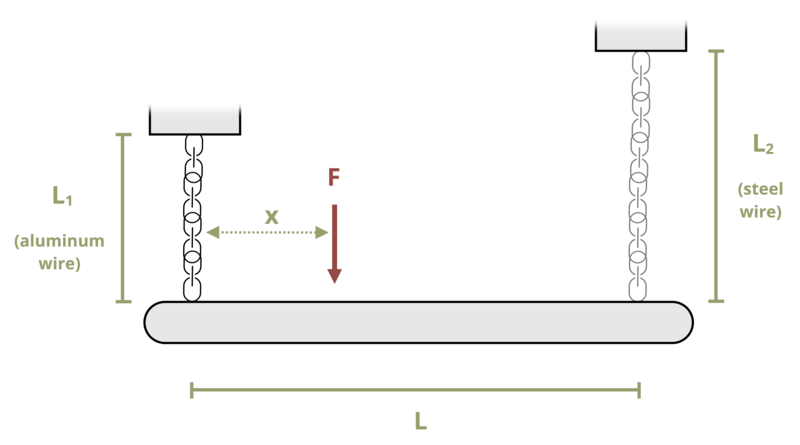
\includegraphics[keepaspectratio]{images/191.png}}
{[}Problem adapted from © Kurt Gramoll CC BY NC-SA 4.0{]}

\begin{Shaded}
\begin{Highlighting}[]
\NormalTok{\#| standalone: true}
\NormalTok{\#| viewerHeight: 600}
\NormalTok{\#| components: [viewer]}

\NormalTok{from shiny import App, render, ui, reactive}
\NormalTok{import random}
\NormalTok{import asyncio}
\NormalTok{import io}
\NormalTok{import math}
\NormalTok{import string}
\NormalTok{from datetime import datetime}
\NormalTok{from pathlib import Path}

\NormalTok{def generate\_random\_letters(length):}
\NormalTok{    \# Generate a random string of letters of specified length}
\NormalTok{    return \textquotesingle{}\textquotesingle{}.join(random.choice(string.ascii\_lowercase) for \_ in range(length))}

\NormalTok{problem\_ID="191"}
\NormalTok{L1=reactive.Value("\_\_")}
\NormalTok{L2=reactive.Value("\_\_")}
\NormalTok{F=reactive.Value("\_\_")}
\NormalTok{A=reactive.Value("\_\_")}
\NormalTok{L=reactive.Value("\_\_")}
\NormalTok{Esteel = 29000}
\NormalTok{Ealuminum = 10000}


\NormalTok{attempts=["Timestamp,Attempt,Answer,Feedback\textbackslash{}n"]}

\NormalTok{app\_ui = ui.page\_fluid(}
\NormalTok{    \#ui.markdown("**Please enter your ID number from your instructor and click to generate your problem**"),}
\NormalTok{    \#ui.input\_text("ID","", placeholder="Enter ID Number Here"),}
\NormalTok{    \#ui.input\_action\_button("generate\_problem", "Generate Problem", class\_="btn{-}primary"),}
\NormalTok{    ui.markdown("**Problem Statement**"),}
\NormalTok{    ui.output\_ui("ui\_problem\_statement"),}
\NormalTok{    ui.input\_text("answer","Your Answer in units of inches", placeholder="Please enter your answer"),}
\NormalTok{    ui.input\_action\_button("submit", "Check Answer", class\_="btn{-}primary"),}
\NormalTok{    \#ui.download\_button("download", "Download File to Submit", class\_="btn{-}success"),}
\NormalTok{)}


\NormalTok{def server(input, output, session):}
\NormalTok{    \# Initialize a counter for attempts}
\NormalTok{    attempt\_counter = reactive.Value(0)}

\NormalTok{    @output}
\NormalTok{    @render.ui}
\NormalTok{    def ui\_problem\_statement():}
\NormalTok{        randomize\_vars()}
\NormalTok{        return[ui.markdown(f"A bar is attached to two wires, one steel and one aluminum. If the lengths of the wires L\textless{}sub\textgreater{}1\textless{}/sub\textgreater{} = \{L1()\} in. and L\textless{}sub\textgreater{}2\textless{}/sub\textgreater{} = \{L2()\} in., find the distance x that load F = \{F()\} kips must be placed at so that the bar remains horizontal after the load is applied. Both wires have the same cross{-}section area A = \{A()\} in.\textless{}sup\textgreater{}2\textless{}/sup\textgreater{}. Assume E\textless{}sub\textgreater{}steel\textless{}/sub\textgreater{} = 29,000 ksi, E\textless{}sub\textgreater{}aluminum\textless{}/sub\textgreater{} = 10,000 ksi and that the bar is of length L = \{L()\} in.")]}
    
\NormalTok{    \#@reactive.Effect}
\NormalTok{    \#@reactive.event(input.generate\_problem)}
\NormalTok{    def randomize\_vars():}
\NormalTok{        random.seed(101)}
\NormalTok{        L1.set(random.randrange(50, 150, 1)/10)}
\NormalTok{        L2.set(round(L1()*2, 2))}
\NormalTok{        F.set(random.randrange(30, 150, 1)/10)}
\NormalTok{        A.set(random.randrange(2, 25, 1)/100)}
\NormalTok{        L.set(random.randrange(10, 20, 1))}
        
\NormalTok{    @reactive.Effect}
\NormalTok{    @reactive.event(input.submit)}
\NormalTok{    def \_():}
\NormalTok{        attempt\_counter.set(attempt\_counter() + 1)  \# Increment the attempt counter on each submission.}
\NormalTok{        PsPa = (L1()*Esteel*A())/(L2()*Ealuminum*A())}
\NormalTok{        Ps = (F()/(PsPa+1))*PsPa}
\NormalTok{        instr=(Ps*L())/F()}
\NormalTok{        if math.isclose(float(input.answer()), instr, rel\_tol=0.01):}
\NormalTok{            check = "*Correct*"}
\NormalTok{            correct\_indicator = "JL"}
\NormalTok{        else:}
\NormalTok{            check = "*Not Correct.*"}
\NormalTok{            correct\_indicator = "JG"}

\NormalTok{        \# Generate random parts for the encoded attempt.}
\NormalTok{        random\_start = generate\_random\_letters(4)}
\NormalTok{        random\_middle = generate\_random\_letters(4)}
\NormalTok{        random\_end = generate\_random\_letters(4)}
\NormalTok{        \#encoded\_attempt = f"\{random\_start\}\{problem\_ID\}{-}\{random\_middle\}\{attempt\_counter()\}\{correct\_indicator\}{-}\{random\_end\}\{input.ID()\}"}

\NormalTok{        \# Store the most recent encoded attempt in a reactive value so it persists across submissions}
\NormalTok{        \#session.encoded\_attempt = reactive.Value(encoded\_attempt)}

\NormalTok{        \# Append the attempt data to the attempts list without the encoded attempt}
\NormalTok{        attempts.append(f"\{datetime.now()\}, \{attempt\_counter()\}, \{input.answer()\}, \{check\}\textbackslash{}n")}

\NormalTok{        \# Show feedback to the user.}
\NormalTok{        feedback = ui.markdown(f"Your answer of \{input.answer()\} is \{check\}.")}
\NormalTok{        m = ui.modal(}
\NormalTok{            feedback,}
\NormalTok{            title="Feedback",}
\NormalTok{            easy\_close=True}
\NormalTok{        )}
\NormalTok{        ui.modal\_show(m)}

\NormalTok{    \#@render.download(filename=lambda: f"Problem\_Log{-}\{problem\_ID\}{-}\{input.ID()\}.csv")}
\NormalTok{    async def download():}
\NormalTok{        \# Start the CSV with the encoded attempt (without label)}
\NormalTok{        final\_encoded = session.encoded\_attempt() if session.encoded\_attempt is not None else "No attempts"}
\NormalTok{        yield f"\{final\_encoded\}\textbackslash{}n\textbackslash{}n"}
        
\NormalTok{        \# Write the header for the remaining CSV data once}
\NormalTok{        yield "Timestamp,Attempt,Answer,Feedback\textbackslash{}n"}
        
\NormalTok{        \# Write the attempts data, ensure that the header from the attempts list is not written again}
\NormalTok{        for attempt in attempts[1:]:  \# Skip the first element which is the header}
\NormalTok{            await asyncio.sleep(0.25)  \# This delay may not be necessary; adjust as needed}
\NormalTok{            yield attempt}


\NormalTok{\# App installation}
\NormalTok{app = App(app\_ui, server)}
\end{Highlighting}
\end{Shaded}

\chapter*{Problem 5.28 - Deformation in Systems of
Bars}\label{problem-5.28---deformation-in-systems-of-bars}
\addcontentsline{toc}{chapter}{Problem 5.28 - Deformation in Systems of
Bars}

\markboth{Problem 5.28 - Deformation in Systems of Bars}{Problem 5.28 -
Deformation in Systems of Bars}

\pandocbounded{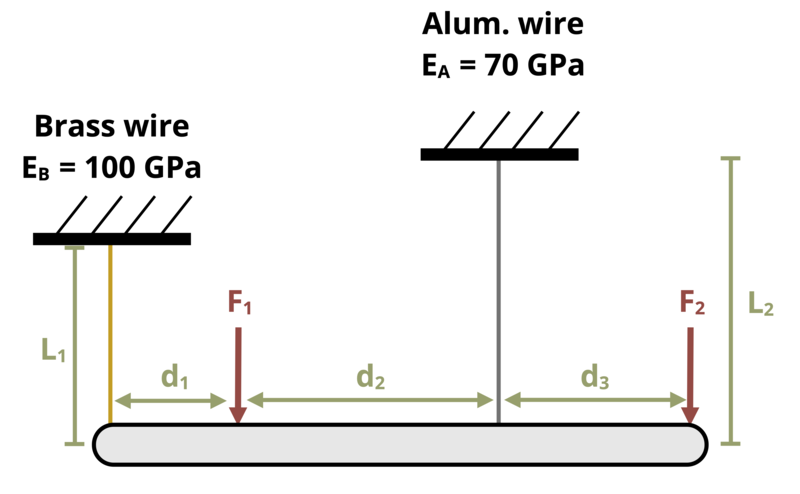
\includegraphics[keepaspectratio]{images/202.png}}
{[}Problem adapted from © Kurt Gramoll CC BY NC-SA 4.0{]}

\begin{Shaded}
\begin{Highlighting}[]
\NormalTok{\#| standalone: true}
\NormalTok{\#| viewerHeight: 600}
\NormalTok{\#| components: [viewer]}

\NormalTok{from shiny import App, render, ui, reactive}
\NormalTok{import random}
\NormalTok{import asyncio}
\NormalTok{import io}
\NormalTok{import math}
\NormalTok{import string}
\NormalTok{from datetime import datetime}
\NormalTok{from pathlib import Path}

\NormalTok{def generate\_random\_letters(length):}
\NormalTok{    \# Generate a random string of letters of specified length}
\NormalTok{    return \textquotesingle{}\textquotesingle{}.join(random.choice(string.ascii\_lowercase) for \_ in range(length))  }

\NormalTok{problem\_ID="202"}
\NormalTok{db=reactive.Value("\_\_")}
\NormalTok{da=reactive.Value("\_\_")}
\NormalTok{F1=reactive.Value("\_\_")}
\NormalTok{F2=reactive.Value("\_\_")}
  
\NormalTok{attempts=["Timestamp,Attempt,Answer,Feedback\textbackslash{}n"]}

\NormalTok{app\_ui = ui.page\_fluid(}
\NormalTok{    \#ui.markdown("**Please enter your ID number from your instructor and click to generate your problem**"),}
\NormalTok{    \#ui.input\_text("ID","", placeholder="Enter ID Number Here"),}
\NormalTok{    \#ui.input\_action\_button("generate\_problem", "Generate Problem", class\_="btn{-}primary"),}
\NormalTok{    ui.markdown("**Problem Statement**"),}
\NormalTok{    ui.output\_ui("ui\_problem\_statement"),}
\NormalTok{    ui.input\_text("answer","Your Answer in units of degrees", placeholder="Please enter your answer"),}
\NormalTok{    ui.input\_action\_button("submit", "Check Answer", class\_="btn{-}primary"),}
\NormalTok{    \#ui.download\_button("download", "Download File to Submit", class\_="btn{-}success"),}
\NormalTok{)}

\NormalTok{def server(input, output, session):}
\NormalTok{    \# Initialize a counter for attempts}
\NormalTok{    attempt\_counter = reactive.Value(0)}

\NormalTok{    @output}
\NormalTok{    @render.ui}
\NormalTok{    def ui\_problem\_statement():}
\NormalTok{        randomize\_vars()}
\NormalTok{        return[ui.markdown(f"A bar is attached to two wires, one brass (diameter d\textless{}sub\textgreater{}b\textless{}/sub\textgreater{} = \{db()\} mm) and one aluminum (diameter d\textless{}sub\textgreater{}a\textless{}/sub\textgreater{} = \{da()\} mm). Loads F\textless{}sub\textgreater{}1\textless{}/sub\textgreater{} = \{F1()\} kN and F\textless{}sub\textgreater{}2\textless{}/sub\textgreater{} = \{F2()\} kN are applied as shown. Determine the angle of the bar from horizontal after the loads are applied.")]}
    
\NormalTok{    \#@reactive.Effect}
\NormalTok{    \#@reactive.event(input.generate\_problem)}
\NormalTok{    def randomize\_vars():}
\NormalTok{        random.seed(101)}
\NormalTok{        db.set(random.randrange(32,60,2))}
\NormalTok{        da.set(random.randrange(20,30,2))}
\NormalTok{        F1.set(random.randrange(10,50,1))}
\NormalTok{        F2.set(random.randrange(10,50,1))}

\NormalTok{    @reactive.Effect}
\NormalTok{    @reactive.event(input.submit)}
\NormalTok{    def \_():}
\NormalTok{        attempt\_counter.set(attempt\_counter() + 1)  \# Increment the attempt counter on each submission.}
\NormalTok{        FA = (2*F1()+10*F2())/7}
\NormalTok{        FB = F1()+F2(){-}FA}
\NormalTok{        EB = 100*10**9}
\NormalTok{        EA = 70*10**9}
\NormalTok{        delB = FB*1000*0.04/((db()/2000)**2*math.pi*EB)}
\NormalTok{        delA = FA*1000*0.06/((da()/2000)**2*math.pi*EA)}
\NormalTok{        instr = math.atan((delA{-}delB)/0.07)*180/math.pi}
        
\NormalTok{        if math.isclose(float(input.answer()), instr, rel\_tol=0.01):}
\NormalTok{            check = "*Correct*"}
\NormalTok{            correct\_indicator = "JL"}
\NormalTok{        else:}
\NormalTok{            check = "*Not Correct.*"}
\NormalTok{            correct\_indicator = "JG"}

\NormalTok{        \# Generate random parts for the encoded attempt.}
\NormalTok{        random\_start = generate\_random\_letters(4)}
\NormalTok{        random\_middle = generate\_random\_letters(4)}
\NormalTok{        random\_end = generate\_random\_letters(4)}
\NormalTok{        \#encoded\_attempt = f"\{random\_start\}\{problem\_ID\}{-}\{random\_middle\}\{attempt\_counter()\}\{correct\_indicator\}{-}\{random\_end\}\{input.ID()\}"}

\NormalTok{        \# Store the most recent encoded attempt in a reactive value so it persists across submissions}
\NormalTok{        \#session.encoded\_attempt = reactive.Value(encoded\_attempt)}

\NormalTok{        \# Append the attempt data to the attempts list without the encoded attempt}
\NormalTok{        attempts.append(f"\{datetime.now()\}, \{attempt\_counter()\}, \{input.answer()\}, \{check\}\textbackslash{}n")}

\NormalTok{        \# Show feedback to the user.}
\NormalTok{        feedback = ui.markdown(f"Your answer of \{input.answer()\} is \{check\}.")}
\NormalTok{        m = ui.modal(}
\NormalTok{            feedback,}
\NormalTok{            title="Feedback",}
\NormalTok{            easy\_close=True}
\NormalTok{        )}
\NormalTok{        ui.modal\_show(m)}

\NormalTok{    \#@render.download(filename=lambda: f"Problem\_Log{-}\{problem\_ID\}{-}\{input.ID()\}.csv")}
\NormalTok{    async def download():}
\NormalTok{        \# Start the CSV with the encoded attempt (without label)}
\NormalTok{        final\_encoded = session.encoded\_attempt() if session.encoded\_attempt is not None else "No attempts"}
\NormalTok{        yield f"\{final\_encoded\}\textbackslash{}n\textbackslash{}n"}
        
\NormalTok{        \# Write the header for the remaining CSV data once}
\NormalTok{        yield "Timestamp,Attempt,Answer,Feedback\textbackslash{}n"}
        
\NormalTok{        \# Write the attempts data, ensure that the header from the attempts list is not written again}
\NormalTok{        for attempt in attempts[1:]:  \# Skip the first element which is the header}
\NormalTok{            await asyncio.sleep(0.25)  \# This delay may not be necessary; adjust as needed}
\NormalTok{            yield attempt}

\NormalTok{\# App installation}
\NormalTok{app = App(app\_ui, server)}
\end{Highlighting}
\end{Shaded}

\chapter*{Problem 5.33 - Deformation in Systems of
Bars}\label{problem-5.33---deformation-in-systems-of-bars}
\addcontentsline{toc}{chapter}{Problem 5.33 - Deformation in Systems of
Bars}

\markboth{Problem 5.33 - Deformation in Systems of Bars}{Problem 5.33 -
Deformation in Systems of Bars}

\pandocbounded{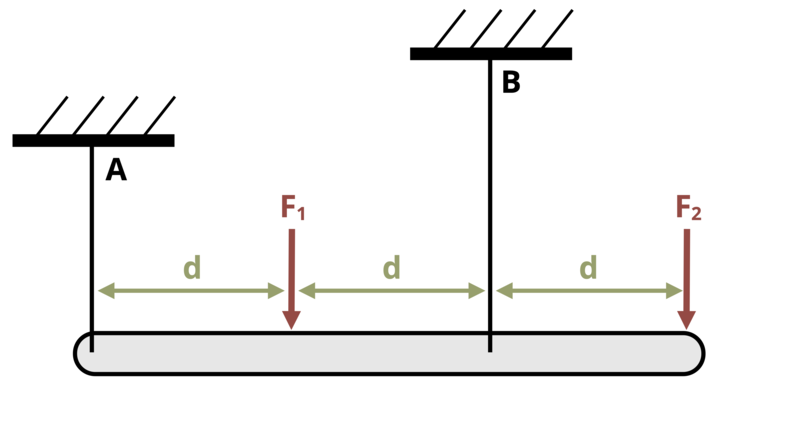
\includegraphics[keepaspectratio]{images/189.png}}
{[}Problem adapted from © Kurt Gramoll CC BY NC-SA 4.0{]}

\begin{Shaded}
\begin{Highlighting}[]
\NormalTok{\#| standalone: true}
\NormalTok{\#| viewerHeight: 600}
\NormalTok{\#| components: [viewer]}

\NormalTok{from shiny import App, render, ui, reactive}
\NormalTok{import random}
\NormalTok{import asyncio}
\NormalTok{import io}
\NormalTok{import math}
\NormalTok{import string}
\NormalTok{from datetime import datetime}
\NormalTok{from pathlib import Path}

\NormalTok{def generate\_random\_letters(length):}
\NormalTok{    \# Generate a random string of letters of specified length}
\NormalTok{    return \textquotesingle{}\textquotesingle{}.join(random.choice(string.ascii\_lowercase) for \_ in range(length))  }
\NormalTok{problem\_ID="189"}
\NormalTok{F1=reactive.Value("\_\_")}
\NormalTok{F2=reactive.Value("\_\_")}
\NormalTok{AA=reactive.Value("\_\_")}
\NormalTok{AB=reactive.Value("\_\_")}
\NormalTok{EA=reactive.Value("\_\_")}
\NormalTok{EB=reactive.Value("\_\_")}
  
\NormalTok{attempts=["Timestamp,Attempt,Answer,Feedback\textbackslash{}n"]}

\NormalTok{app\_ui = ui.page\_fluid(}
\NormalTok{    \#ui.markdown("**Please enter your ID number from your instructor and click to generate your problem**"),}
\NormalTok{    \#ui.input\_text("ID","", placeholder="Enter ID Number Here"),}
\NormalTok{    \#ui.input\_action\_button("generate\_problem", "Generate Problem", class\_="btn{-}primary"),}
\NormalTok{    ui.markdown("**Problem Statement**"),}
\NormalTok{    ui.output\_ui("ui\_problem\_statement"),}
\NormalTok{    ui.input\_text("answer","Your Answer in units of degrees", placeholder="Please enter your answer"),}
\NormalTok{    ui.input\_action\_button("submit", "Check Answer", class\_="btn{-}primary"),}
\NormalTok{    \#ui.download\_button("download", "Download File to Submit", class\_="btn{-}success"),}
\NormalTok{)}

\NormalTok{def server(input, output, session):}
\NormalTok{    \# Initialize a counter for attempts}
\NormalTok{    attempt\_counter = reactive.Value(0)}

\NormalTok{    @output}
\NormalTok{    @render.ui}
\NormalTok{    def ui\_problem\_statement():}
\NormalTok{        randomize\_vars()}
\NormalTok{        return[ui.markdown(f"Two loads, F\textless{}sub\textgreater{}1\textless{}/sub\textgreater{} = \{F1()\} lb and F\textless{}sub\textgreater{}2\textless{}/sub\textgreater{} = \{F2()\} lb are applied to a rigid horizontal rod that is supported by two wires. Wire A has cross{-}sectional area A\textless{}sub\textgreater{}A\textless{}/sub\textgreater{} = \{AA()\} in.\textless{}sup\textgreater{}2\textless{}/sup\textgreater{} and elastic modulus E\textless{}sub\textgreater{}A\textless{}/sub\textgreater{} = \{EA()\}x10\textless{}sup\textgreater{}6\textless{}/sup\textgreater{} psi. Wire B has cross{-}sectional area A\textless{}sub\textgreater{}B\textless{}/sub\textgreater{} = \{AB()\} in.\textless{}sup\textgreater{}2\textless{}/sup\textgreater{} and elastic modulus E\textless{}sub\textgreater{}B\textless{}/sub\textgreater{} = \{EB()\}x10\textless{}sup\textgreater{}6\textless{}/sup\textgreater{} psi. Determine the angle of rotation after the loads are applied")]}
    
\NormalTok{    \#@reactive.Effect}
\NormalTok{    \#@reactive.event(input.generate\_problem)}
\NormalTok{    def randomize\_vars():}
\NormalTok{        random.seed(101)}
\NormalTok{        F1.set(random.randrange(200,800,10))}
\NormalTok{        F2.set(random.randrange(200,800,10))}
\NormalTok{        AA.set(random.randrange(5,10,1)/100)}
\NormalTok{        AB.set(random.randrange(2,5,1)/100)}
\NormalTok{        EA.set(random.randrange(15,25,1))}
\NormalTok{        EB.set(random.randrange(5,14,1))}
        
\NormalTok{    @reactive.Effect}
\NormalTok{    @reactive.event(input.submit)}
\NormalTok{    def \_():}
\NormalTok{        attempt\_counter.set(attempt\_counter() + 1)  \# Increment the attempt counter on each submission.}
\NormalTok{        FB = (F1()*8+F2()*24)/16}
\NormalTok{        FA = F1()+F2(){-}FB}
\NormalTok{        delB = FB*12/(EB()*10**6*AB())}
\NormalTok{        delA = FA*6/(EA()*10**6*AA())}
\NormalTok{        delta = delB{-}delA}
\NormalTok{        instr = math.atan(delta/16)*180/math.pi}
        
\NormalTok{        if math.isclose(float(input.answer()), instr, rel\_tol=0.01):}
\NormalTok{            check = "*Correct*"}
\NormalTok{            correct\_indicator = "JL"}
\NormalTok{        else:}
\NormalTok{            check = "*Not Correct.*"}
\NormalTok{            correct\_indicator = "JG"}

\NormalTok{        \# Generate random parts for the encoded attempt.}
\NormalTok{        random\_start = generate\_random\_letters(4)}
\NormalTok{        random\_middle = generate\_random\_letters(4)}
\NormalTok{        random\_end = generate\_random\_letters(4)}
\NormalTok{        \#encoded\_attempt = f"\{random\_start\}\{problem\_ID\}{-}\{random\_middle\}\{attempt\_counter()\}\{correct\_indicator\}{-}\{random\_end\}\{input.ID()\}"}

\NormalTok{        \# Store the most recent encoded attempt in a reactive value so it persists across submissions}
\NormalTok{        \#session.encoded\_attempt = reactive.Value(encoded\_attempt)}

\NormalTok{        \# Append the attempt data to the attempts list without the encoded attempt}
\NormalTok{        attempts.append(f"\{datetime.now()\}, \{attempt\_counter()\}, \{input.answer()\}, \{check\}\textbackslash{}n")}

\NormalTok{        \# Show feedback to the user.}
\NormalTok{        feedback = ui.markdown(f"Your answer of \{input.answer()\} is \{check\}.")}
\NormalTok{        m = ui.modal(}
\NormalTok{            feedback,}
\NormalTok{            title="Feedback",}
\NormalTok{            easy\_close=True}
\NormalTok{        )}
\NormalTok{        ui.modal\_show(m)}

\NormalTok{    \#@render.download(filename=lambda: f"Problem\_Log{-}\{problem\_ID\}{-}\{input.ID()\}.csv")}
\NormalTok{    async def download():}
\NormalTok{        \# Start the CSV with the encoded attempt (without label)}
\NormalTok{        final\_encoded = session.encoded\_attempt() if session.encoded\_attempt is not None else "No attempts"}
\NormalTok{        yield f"\{final\_encoded\}\textbackslash{}n\textbackslash{}n"}
        
\NormalTok{        \# Write the header for the remaining CSV data once}
\NormalTok{        yield "Timestamp,Attempt,Answer,Feedback\textbackslash{}n"}
        
\NormalTok{        \# Write the attempts data, ensure that the header from the attempts list is not written again}
\NormalTok{        for attempt in attempts[1:]:  \# Skip the first element which is the header}
\NormalTok{            await asyncio.sleep(0.25)  \# This delay may not be necessary; adjust as needed}
\NormalTok{            yield attempt}

\NormalTok{\# App installation}
\NormalTok{app = App(app\_ui, server)}
\end{Highlighting}
\end{Shaded}

\chapter*{Problem 5.34 - Statically Indeterminate Axial
Loads}\label{problem-5.34---statically-indeterminate-axial-loads}
\addcontentsline{toc}{chapter}{Problem 5.34 - Statically Indeterminate
Axial Loads}

\markboth{Problem 5.34 - Statically Indeterminate Axial Loads}{Problem
5.34 - Statically Indeterminate Axial Loads}

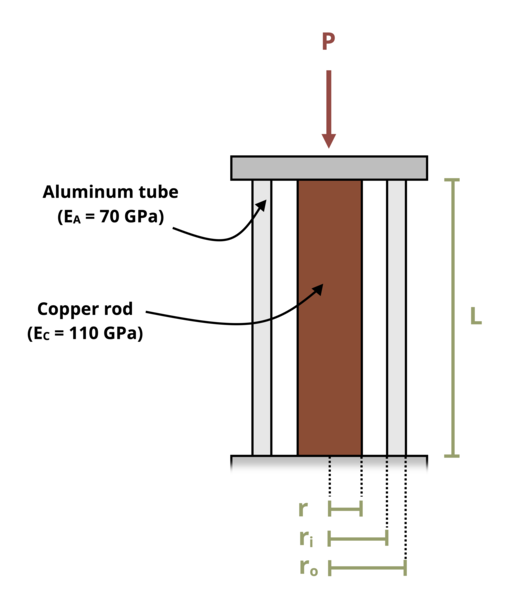
\includegraphics[width=3.64583in,height=\textheight,keepaspectratio]{images/192.png}
{[}Problem adapted from © Kurt Gramoll CC BY NC-SA 4.0{]}

\begin{Shaded}
\begin{Highlighting}[]
\NormalTok{\#| standalone: true}
\NormalTok{\#| viewerHeight: 600}
\NormalTok{\#| components: [viewer]}

\NormalTok{from shiny import App, render, ui, reactive}
\NormalTok{import random}
\NormalTok{import asyncio}
\NormalTok{import io}
\NormalTok{import math}
\NormalTok{import string}
\NormalTok{from datetime import datetime}
\NormalTok{from pathlib import Path}

\NormalTok{def generate\_random\_letters(length):}
\NormalTok{    \# Generate a random string of letters of specified length}
\NormalTok{    return \textquotesingle{}\textquotesingle{}.join(random.choice(string.ascii\_lowercase) for \_ in range(length)) }

\NormalTok{problem\_ID="192"}
\NormalTok{r=reactive.Value("\_\_")}
\NormalTok{ri=reactive.Value("\_\_")}
\NormalTok{ro=reactive.Value("\_\_")}
\NormalTok{L=reactive.Value("\_\_")}
\NormalTok{dL=reactive.Value("\_\_")}
\NormalTok{Ecopper = 110}
\NormalTok{Ealuminum = 70}

\NormalTok{attempts=["Timestamp,Attempt,Answer,Feedback\textbackslash{}n"]}

\NormalTok{app\_ui = ui.page\_fluid(}
\NormalTok{    \#ui.markdown("**Please enter your ID number from your instructor and click to generate your problem**"),}
\NormalTok{    \#ui.input\_text("ID","", placeholder="Enter ID Number Here"),}
\NormalTok{    \#ui.input\_action\_button("generate\_problem", "Generate Problem", class\_="btn{-}primary"),}
\NormalTok{    ui.markdown("**Problem Statement**"),}
\NormalTok{    ui.output\_ui("ui\_problem\_statement"),}
\NormalTok{    ui.input\_text("answer","Your Answer in units of kN", placeholder="Please enter your answer"),}
\NormalTok{    ui.input\_action\_button("submit", "Check Answer", class\_="btn{-}primary"),}
\NormalTok{    \#ui.download\_button("download", "Download File to Submit", class\_="btn{-}success"),}
\NormalTok{)}

\NormalTok{def server(input, output, session):}
\NormalTok{    \# Initialize a counter for attempts}
\NormalTok{    attempt\_counter = reactive.Value(0)}

\NormalTok{    @output}
\NormalTok{    @render.ui}
\NormalTok{    def ui\_problem\_statement():}
\NormalTok{        randomize\_vars()}
\NormalTok{        return[ui.markdown(f"A copper circular rod of radius r = \{r()\} cm is inserted into an aluminum tube with inner radius r\textless{}sub\textgreater{}i\textless{}/sub\textgreater{} = \{ri()\} cm and outer radius r\textless{}sub\textgreater{}o\textless{}/sub\textgreater{} = \{ro()\} cm as shown. Load P is applied to the rigid top plate. If length L = \{L()\} cm, what load P will cause the plate to deflect dL = \{dL()\} mm downward? Assume E\textless{}sub\textgreater{}copper\textless{}/sub\textgreater{} = 110 GPa and E\textless{}sub\textgreater{}aluminum\textless{}/sub\textgreater{} = 70 GPa")]}
    
\NormalTok{    \#@reactive.Effect}
\NormalTok{    \#@reactive.event(input.generate\_problem)}
\NormalTok{    def randomize\_vars():}
\NormalTok{        random.seed(101)}
\NormalTok{        r.set(random.randrange(20, 60, 1)/10)}
\NormalTok{        ri.set(round(r()*1.25, 2))}
\NormalTok{        ro.set(round(r()*1.5, 2))}
\NormalTok{        L.set(random.randrange(150, 300, 1)/10)}
\NormalTok{        dL.set(random.randrange(10, 50, 1)/100)}
        
\NormalTok{    @reactive.Effect}
\NormalTok{    @reactive.event(input.submit)}
\NormalTok{    def \_():}
\NormalTok{        attempt\_counter.set(attempt\_counter() + 1)  \# Increment the attempt counter on each submission.}
\NormalTok{        instr=(((dL()*Ecopper*r()**2*math.pi)/L()) + ((dL()*Ealuminum*(ro()**2{-}ri()**2)*math.pi)/L()))*10}
\NormalTok{        if math.isclose(float(input.answer()), instr, rel\_tol=0.01):}
\NormalTok{            check = "*Correct*"}
\NormalTok{            correct\_indicator = "JL"}
\NormalTok{        else:}
\NormalTok{            check = "*Not Correct.*"}
\NormalTok{            correct\_indicator = "JG"}

\NormalTok{        \# Generate random parts for the encoded attempt.}
\NormalTok{        random\_start = generate\_random\_letters(4)}
\NormalTok{        random\_middle = generate\_random\_letters(4)}
\NormalTok{        random\_end = generate\_random\_letters(4)}
\NormalTok{        \#encoded\_attempt = f"\{random\_start\}\{problem\_ID\}{-}\{random\_middle\}\{attempt\_counter()\}\{correct\_indicator\}{-}\{random\_end\}\{input.ID()\}"}

\NormalTok{        \# Store the most recent encoded attempt in a reactive value so it persists across submissions}
\NormalTok{        \#session.encoded\_attempt = reactive.Value(encoded\_attempt)}

\NormalTok{        \# Append the attempt data to the attempts list without the encoded attempt}
\NormalTok{        attempts.append(f"\{datetime.now()\}, \{attempt\_counter()\}, \{input.answer()\}, \{check\}\textbackslash{}n")}

\NormalTok{        \# Show feedback to the user.}
\NormalTok{        feedback = ui.markdown(f"Your answer of \{input.answer()\} is \{check\}.")}
\NormalTok{        m = ui.modal(}
\NormalTok{            feedback,}
\NormalTok{            title="Feedback",}
\NormalTok{            easy\_close=True}
\NormalTok{        )}
\NormalTok{        ui.modal\_show(m)}

\NormalTok{    \#@render.download(filename=lambda: f"Problem\_Log{-}\{problem\_ID\}{-}\{input.ID()\}.csv")}
\NormalTok{    async def download():}
\NormalTok{        \# Start the CSV with the encoded attempt (without label)}
\NormalTok{        final\_encoded = session.encoded\_attempt() if session.encoded\_attempt is not None else "No attempts"}
\NormalTok{        yield f"\{final\_encoded\}\textbackslash{}n\textbackslash{}n"}
        
\NormalTok{        \# Write the header for the remaining CSV data once}
\NormalTok{        yield "Timestamp,Attempt,Answer,Feedback\textbackslash{}n"}
        
\NormalTok{        \# Write the attempts data, ensure that the header from the attempts list is not written again}
\NormalTok{        for attempt in attempts[1:]:  \# Skip the first element which is the header}
\NormalTok{            await asyncio.sleep(0.25)  \# This delay may not be necessary; adjust as needed}
\NormalTok{            yield attempt}

\NormalTok{\# App installation}
\NormalTok{app = App(app\_ui, server)}
\end{Highlighting}
\end{Shaded}

\chapter*{Problem 5.35 - Statically Indeterminate Axial
Loads}\label{problem-5.35---statically-indeterminate-axial-loads}
\addcontentsline{toc}{chapter}{Problem 5.35 - Statically Indeterminate
Axial Loads}

\markboth{Problem 5.35 - Statically Indeterminate Axial Loads}{Problem
5.35 - Statically Indeterminate Axial Loads}

\pandocbounded{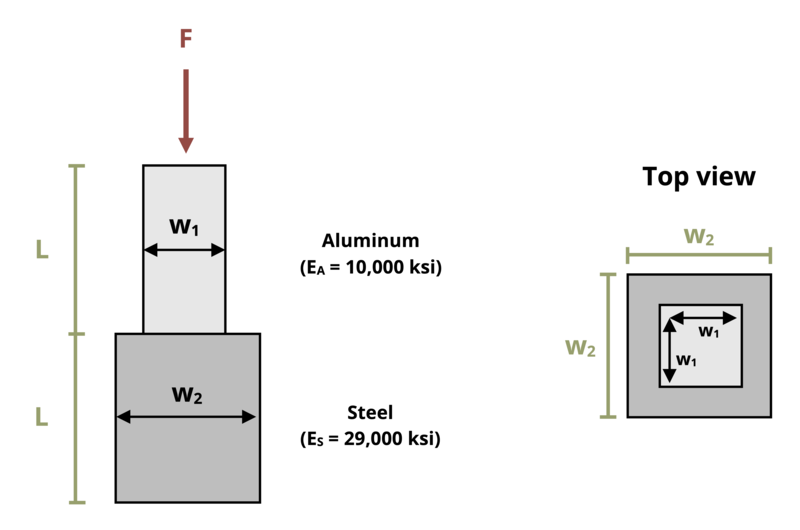
\includegraphics[keepaspectratio]{images/193.png}}
{[}Problem adapted from © Kurt Gramoll CC BY NC-SA 4.0{]}

\begin{Shaded}
\begin{Highlighting}[]
\NormalTok{\#| standalone: true}
\NormalTok{\#| viewerHeight: 600}
\NormalTok{\#| components: [viewer]}

\NormalTok{from shiny import App, render, ui, reactive}
\NormalTok{import random}
\NormalTok{import asyncio}
\NormalTok{import io}
\NormalTok{import math}
\NormalTok{import string}
\NormalTok{from datetime import datetime}
\NormalTok{from pathlib import Path}

\NormalTok{def generate\_random\_letters(length):}
\NormalTok{    \# Generate a random string of letters of specified length}
\NormalTok{    return \textquotesingle{}\textquotesingle{}.join(random.choice(string.ascii\_lowercase) for \_ in range(length)) }

\NormalTok{problem\_ID="193"}
\NormalTok{F=reactive.Value("\_\_")}
\NormalTok{w1=reactive.Value("\_\_")}
\NormalTok{w2=reactive.Value("\_\_")}
\NormalTok{L=reactive.Value("\_\_")}
\NormalTok{Esteel = 29000}
\NormalTok{Ealuminum = 10000}



\NormalTok{attempts=["Timestamp,Attempt,Answer,Feedback\textbackslash{}n"]}

\NormalTok{app\_ui = ui.page\_fluid(}
\NormalTok{    \#ui.markdown("**Please enter your ID number from your instructor and click to generate your problem**"),}
\NormalTok{    \#ui.input\_text("ID","", placeholder="Enter ID Number Here"),}
\NormalTok{    \#ui.input\_action\_button("generate\_problem", "Generate Problem", class\_="btn{-}primary"),}
\NormalTok{    ui.markdown("**Problem Statement**"),}
\NormalTok{    ui.output\_ui("ui\_problem\_statement"),}
\NormalTok{    ui.input\_text("answer","Your Answer in units of inches", placeholder="Please enter your answer"),}
\NormalTok{    ui.input\_action\_button("submit", "Check Answer", class\_="btn{-}primary"),}
\NormalTok{    \#ui.download\_button("download", "Download File to Submit", class\_="btn{-}success"),}
\NormalTok{)}


\NormalTok{def server(input, output, session):}
\NormalTok{    \# Initialize a counter for attempts}
\NormalTok{    attempt\_counter = reactive.Value(0)}

\NormalTok{    @output}
\NormalTok{    @render.ui}
\NormalTok{    def ui\_problem\_statement():}
\NormalTok{        randomize\_vars()}
\NormalTok{        return[ui.markdown(f"Two blocks with square cross{-}sections are stacked as shown, with the top block inserted into the bottom block and subjected to load F = \{F()\} kips. The top block is aluminum (E = 10,000 ksi) with side length w\textless{}sub\textgreater{}1\textless{}/sub\textgreater{} = \{w1()\} in.  and the bottom block is steel (E = 29,000 ksi) with side length w\textless{}sub\textgreater{}2\textless{}/sub\textgreater{} = \{w2()\} in. If length L = \{L()\} in., what is the total deflection of the top surface? Ignore the weight of the blocks. ")]}
    
\NormalTok{    \#@reactive.Effect}
\NormalTok{    \#@reactive.event(input.generate\_problem)}
\NormalTok{    def randomize\_vars():}
\NormalTok{        random.seed(101)}
\NormalTok{        F.set(random.randrange(20, 100, 1)/10)}
\NormalTok{        w1.set(random.randrange(15, 50, 1)/10)}
\NormalTok{        w2.set(round(w1()*1.5))}
\NormalTok{        L.set(random.randrange(50, 200, 1)/10)}
        
\NormalTok{    @reactive.Effect}
\NormalTok{    @reactive.event(input.submit)}
\NormalTok{    def \_():}
\NormalTok{        attempt\_counter.set(attempt\_counter() + 1)  \# Increment the attempt counter on each submission.}
\NormalTok{        instr=F()*L()*((1/((w1()**2)*Ealuminum)) + (1/((w2()**2)*Esteel)))}
\NormalTok{        if math.isclose(float(input.answer()), instr, rel\_tol=0.01):}
\NormalTok{            check = "*Correct*"}
\NormalTok{            correct\_indicator = "JL"}
\NormalTok{        else:}
\NormalTok{            check = "*Not Correct.*"}
\NormalTok{            correct\_indicator = "JG"}

\NormalTok{        \# Generate random parts for the encoded attempt.}
\NormalTok{        random\_start = generate\_random\_letters(4)}
\NormalTok{        random\_middle = generate\_random\_letters(4)}
\NormalTok{        random\_end = generate\_random\_letters(4)}
\NormalTok{        \#encoded\_attempt = f"\{random\_start\}\{problem\_ID\}{-}\{random\_middle\}\{attempt\_counter()\}\{correct\_indicator\}{-}\{random\_end\}\{input.ID()\}"}

\NormalTok{        \# Store the most recent encoded attempt in a reactive value so it persists across submissions}
\NormalTok{        \#session.encoded\_attempt = reactive.Value(encoded\_attempt)}

\NormalTok{        \# Append the attempt data to the attempts list without the encoded attempt}
\NormalTok{        attempts.append(f"\{datetime.now()\}, \{attempt\_counter()\}, \{input.answer()\}, \{check\}\textbackslash{}n")}

\NormalTok{        \# Show feedback to the user.}
\NormalTok{        feedback = ui.markdown(f"Your answer of \{input.answer()\} is \{check\}.")}
\NormalTok{        m = ui.modal(}
\NormalTok{            feedback,}
\NormalTok{            title="Feedback",}
\NormalTok{            easy\_close=True}
\NormalTok{        )}
\NormalTok{        ui.modal\_show(m)}

\NormalTok{    \#@render.download(filename=lambda: f"Problem\_Log{-}\{problem\_ID\}{-}\{input.ID()\}.csv")}
\NormalTok{    async def download():}
\NormalTok{        \# Start the CSV with the encoded attempt (without label)}
\NormalTok{        final\_encoded = session.encoded\_attempt() if session.encoded\_attempt is not None else "No attempts"}
\NormalTok{        yield f"\{final\_encoded\}\textbackslash{}n\textbackslash{}n"}
        
\NormalTok{        \# Write the header for the remaining CSV data once}
\NormalTok{        yield "Timestamp,Attempt,Answer,Feedback\textbackslash{}n"}
        
\NormalTok{        \# Write the attempts data, ensure that the header from the attempts list is not written again}
\NormalTok{        for attempt in attempts[1:]:  \# Skip the first element which is the header}
\NormalTok{            await asyncio.sleep(0.25)  \# This delay may not be necessary; adjust as needed}
\NormalTok{            yield attempt}


\NormalTok{\# App installation}
\NormalTok{app = App(app\_ui, server)}
\end{Highlighting}
\end{Shaded}

\chapter*{Problem 5.36 - Statically Indeterminate Axial
Loads}\label{problem-5.36---statically-indeterminate-axial-loads}
\addcontentsline{toc}{chapter}{Problem 5.36 - Statically Indeterminate
Axial Loads}

\markboth{Problem 5.36 - Statically Indeterminate Axial Loads}{Problem
5.36 - Statically Indeterminate Axial Loads}

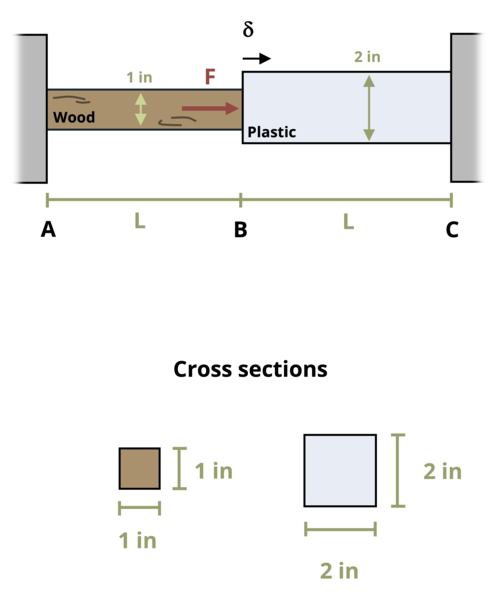
\includegraphics[width=3.64583in,height=\textheight,keepaspectratio]{images/246.png}
{[}Problem adapted from © Kurt Gramoll CC BY NC-SA 4.0{]}

\begin{Shaded}
\begin{Highlighting}[]
\NormalTok{\#| standalone: true}
\NormalTok{\#| viewerHeight: 600}
\NormalTok{\#| components: [viewer]}

\NormalTok{from shiny import App, render, ui, reactive}
\NormalTok{import random}
\NormalTok{import asyncio}
\NormalTok{import io}
\NormalTok{import math}
\NormalTok{import string}
\NormalTok{from datetime import datetime}
\NormalTok{from pathlib import Path}

\NormalTok{def generate\_random\_letters(length):}
\NormalTok{    \# Generate a random string of letters of specified length}
\NormalTok{    return \textquotesingle{}\textquotesingle{}.join(random.choice(string.ascii\_lowercase) for \_ in range(length)) }

\NormalTok{problem\_ID="246"}
\NormalTok{d=reactive.Value("\_\_")}
\NormalTok{L=reactive.Value("\_\_")}
\NormalTok{Eplastic=reactive.Value("\_\_")}
\NormalTok{Ewood=1750}

\NormalTok{attempts=["Timestamp,Attempt,Answer,Feedback\textbackslash{}n"]}

\NormalTok{app\_ui = ui.page\_fluid(}
\NormalTok{    \#ui.markdown("**Please enter your ID number from your instructor and click to generate your problem**"),}
\NormalTok{    \#ui.input\_text("ID","", placeholder="Enter ID Number Here"),}
\NormalTok{    \#ui.input\_action\_button("generate\_problem", "Generate Problem", class\_="btn{-}primary"),}
\NormalTok{    ui.markdown("**Problem Statement**"),}
\NormalTok{    ui.output\_ui("ui\_problem\_statement"),}
\NormalTok{    ui.input\_text("answer","Your Answer in units of lb", placeholder="Please enter your answer"),}
\NormalTok{    ui.input\_action\_button("submit", "Check Answer", class\_="btn{-}primary"),}
\NormalTok{    \#ui.download\_button("download", "Download File to Submit", class\_="btn{-}success"),}
\NormalTok{)}


\NormalTok{def server(input, output, session):}
\NormalTok{    \# Initialize a counter for attempts}
\NormalTok{    attempt\_counter = reactive.Value(0)}

\NormalTok{    @output}
\NormalTok{    @render.ui}
\NormalTok{    def ui\_problem\_statement():}
\NormalTok{        randomize\_vars()}
\NormalTok{        return[ui.markdown(f"Two square members are attached to two fixed walls as shown. Force F is applied at point B and point B is displaced d =  \{d()\} in. to the right. If L = \{L()\} in., E\textless{}sub\textgreater{}wood\textless{}/sub\textgreater{} = 1,750 ksi, and E\textless{}sub\textgreater{}plastic\textless{}/sub\textgreater{} = \{Eplastic()\} ksi, determine the applied force F. ")]}
    
\NormalTok{    \#@reactive.Effect}
\NormalTok{    \#@reactive.event(input.generate\_problem)}
\NormalTok{    def randomize\_vars():}
\NormalTok{        random.seed(101)}
\NormalTok{        d.set(random.randrange(2, 8, 1)/1000)}
\NormalTok{        L.set(random.randrange(4, 15, 1))}
\NormalTok{        Eplastic.set(random.randrange(350, 900, 10))}
       
\NormalTok{    @reactive.Effect}
\NormalTok{    @reactive.event(input.submit)}
\NormalTok{    def \_():}
\NormalTok{        attempt\_counter.set(attempt\_counter() + 1)  \# Increment the attempt counter on each submission.}
\NormalTok{        instr= (d()*1*Ewood*1000)/L() {-} ({-}d()*4*Eplastic()*1000)/L() }
\NormalTok{        if math.isclose(float(input.answer()), instr, rel\_tol=0.01):}
\NormalTok{            check = "*Correct*"}
\NormalTok{            correct\_indicator = "JL"}
\NormalTok{        else:}
\NormalTok{            check = "*Not Correct.*"}
\NormalTok{            correct\_indicator = "JG"}

\NormalTok{        \# Generate random parts for the encoded attempt.}
\NormalTok{        random\_start = generate\_random\_letters(4)}
\NormalTok{        random\_middle = generate\_random\_letters(4)}
\NormalTok{        random\_end = generate\_random\_letters(4)}
\NormalTok{        \#encoded\_attempt = f"\{random\_start\}\{problem\_ID\}{-}\{random\_middle\}\{attempt\_counter()\}\{correct\_indicator\}{-}\{random\_end\}\{input.ID()\}"}

\NormalTok{        \# Store the most recent encoded attempt in a reactive value so it persists across submissions}
\NormalTok{        \#session.encoded\_attempt = reactive.Value(encoded\_attempt)}

\NormalTok{        \# Append the attempt data to the attempts list without the encoded attempt}
\NormalTok{        attempts.append(f"\{datetime.now()\}, \{attempt\_counter()\}, \{input.answer()\}, \{check\}\textbackslash{}n")}

\NormalTok{        \# Show feedback to the user.}
\NormalTok{        feedback = ui.markdown(f"Your answer of \{input.answer()\} is \{check\}.")}
\NormalTok{        m = ui.modal(}
\NormalTok{            feedback,}
\NormalTok{            title="Feedback",}
\NormalTok{            easy\_close=True}
\NormalTok{        )}
\NormalTok{        ui.modal\_show(m)}

\NormalTok{    \#@render.download(filename=lambda: f"Problem\_Log{-}\{problem\_ID\}{-}\{input.ID()\}.csv")}
\NormalTok{    async def download():}
\NormalTok{        \# Start the CSV with the encoded attempt (without label)}
\NormalTok{        final\_encoded = session.encoded\_attempt() if session.encoded\_attempt is not None else "No attempts"}
\NormalTok{        yield f"\{final\_encoded\}\textbackslash{}n\textbackslash{}n"}
        
\NormalTok{        \# Write the header for the remaining CSV data once}
\NormalTok{        yield "Timestamp,Attempt,Answer,Feedback\textbackslash{}n"}
        
\NormalTok{        \# Write the attempts data, ensure that the header from the attempts list is not written again}
\NormalTok{        for attempt in attempts[1:]:  \# Skip the first element which is the header}
\NormalTok{            await asyncio.sleep(0.25)  \# This delay may not be necessary; adjust as needed}
\NormalTok{            yield attempt}

\NormalTok{\# App installation}
\NormalTok{app = App(app\_ui, server)}
\end{Highlighting}
\end{Shaded}

\chapter*{Problem 5.37 - Statically Indeterminate Axial
Loads}\label{problem-5.37---statically-indeterminate-axial-loads}
\addcontentsline{toc}{chapter}{Problem 5.37 - Statically Indeterminate
Axial Loads}

\markboth{Problem 5.37 - Statically Indeterminate Axial Loads}{Problem
5.37 - Statically Indeterminate Axial Loads}

\pandocbounded{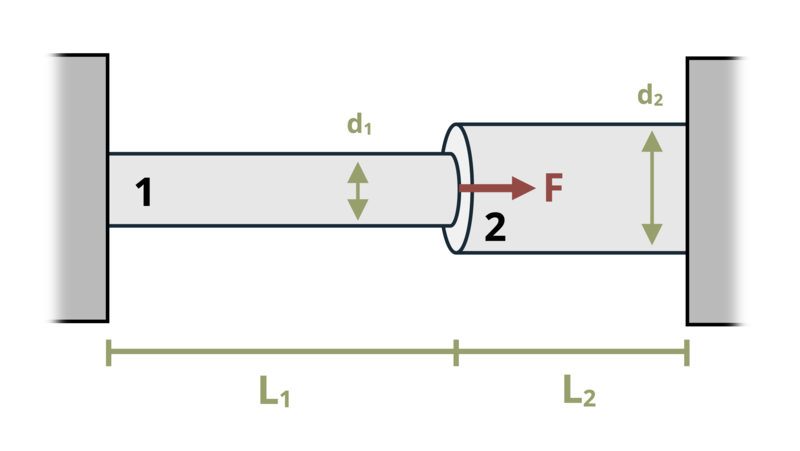
\includegraphics[keepaspectratio]{images/247.png}}
{[}Problem adapted from © Kurt Gramoll CC BY NC-SA 4.0{]}

\begin{Shaded}
\begin{Highlighting}[]
\NormalTok{\#| standalone: true}
\NormalTok{\#| viewerHeight: 600}
\NormalTok{\#| components: [viewer]}

\NormalTok{from shiny import App, render, ui, reactive}
\NormalTok{import random}
\NormalTok{import asyncio}
\NormalTok{import io}
\NormalTok{import math}
\NormalTok{import string}
\NormalTok{from datetime import datetime}
\NormalTok{from pathlib import Path}

\NormalTok{def generate\_random\_letters(length):}
\NormalTok{    \# Generate a random string of letters of specified length}
\NormalTok{    return \textquotesingle{}\textquotesingle{}.join(random.choice(string.ascii\_lowercase) for \_ in range(length)) }

\NormalTok{problem\_ID="247"}
\NormalTok{F=reactive.Value("\_\_")}
\NormalTok{d1=reactive.Value("\_\_")}
\NormalTok{d2=reactive.Value("\_\_")}
\NormalTok{L1=reactive.Value("\_\_")}
\NormalTok{L2=reactive.Value("\_\_")}
\NormalTok{Ewood=70}

\NormalTok{attempts=["Timestamp,Attempt,Answer,Feedback\textbackslash{}n"]}

\NormalTok{app\_ui = ui.page\_fluid(}
\NormalTok{    \#ui.markdown("**Please enter your ID number from your instructor and click to generate your problem**"),}
\NormalTok{    \#ui.input\_text("ID","", placeholder="Enter ID Number Here"),}
\NormalTok{    \#ui.input\_action\_button("generate\_problem", "Generate Problem", class\_="btn{-}primary"),}
\NormalTok{    ui.markdown("**Problem Statement**"),}
\NormalTok{    ui.output\_ui("ui\_problem\_statement"),}
\NormalTok{    ui.input\_text("answer","Your Answer in units of MPa", placeholder="Please enter your answer"),}
\NormalTok{    ui.input\_action\_button("submit", "Check Answer", class\_="btn{-}primary"),}
\NormalTok{    \#ui.download\_button("download", "Download File to Submit", class\_="btn{-}success"),}
\NormalTok{)}


\NormalTok{def server(input, output, session):}
\NormalTok{    \# Initialize a counter for attempts}
\NormalTok{    attempt\_counter = reactive.Value(0)}

\NormalTok{    @output}
\NormalTok{    @render.ui}
\NormalTok{    def ui\_problem\_statement():}
\NormalTok{        randomize\_vars()}
\NormalTok{        return[ui.markdown(f"Two aluminum circular rods are attached to two fixed walls as shown. Assume E = 70 MPa for both cylinders, F = \{F()\} kN, d\textless{}sub\textgreater{}1\textless{}/sub\textgreater{} = \{d1()\} mm, d\textless{}sub\textgreater{}2\textless{}/sub\textgreater{}  = \{d2()\} mm, L\textless{}sub\textgreater{}1\textless{}/sub\textgreater{}  = \{L1()\} mm, and L\textless{}sub\textgreater{}2\textless{}/sub\textgreater{}  = \{L2()\} mm. Determine the normal stress in member 1.")]}
    
\NormalTok{    \#@reactive.Effect}
\NormalTok{    \#@reactive.event(input.generate\_problem)}
\NormalTok{    def randomize\_vars():}
\NormalTok{        random.seed(101)}
\NormalTok{        F.set(random.randrange(20, 100, 1))}
\NormalTok{        d1.set(random.randrange(15, 50, 1))}
\NormalTok{        d2.set(round(d1()*1.5))}
\NormalTok{        L1.set(random.randrange(200, 800, 10))}
\NormalTok{        L2.set(round(L1()*(2/3)))}
       
        
\NormalTok{    @reactive.Effect}
\NormalTok{    @reactive.event(input.submit)}
\NormalTok{    def \_():}
\NormalTok{        attempt\_counter.set(attempt\_counter() + 1)  \# Increment the attempt counter on each submission.}
\NormalTok{        LHS = (L1()/1000)/(math.pi*(d1()/2000)**2) + (L2()/1000)/(math.pi*(d2()/2000)**2)}
\NormalTok{        RHS = (F()*L2())/(math.pi*(d2()/2)**2)}
\NormalTok{        instr= (RHS/LHS)/(math.pi*(d1()/2000)**2)}
\NormalTok{        if math.isclose(float(input.answer()), instr, rel\_tol=0.01):}
\NormalTok{            check = "*Correct*"}
\NormalTok{            correct\_indicator = "JL"}
\NormalTok{        else:}
\NormalTok{            check = "*Not Correct.*"}
\NormalTok{            correct\_indicator = "JG"}

\NormalTok{        \# Generate random parts for the encoded attempt.}
\NormalTok{        random\_start = generate\_random\_letters(4)}
\NormalTok{        random\_middle = generate\_random\_letters(4)}
\NormalTok{        random\_end = generate\_random\_letters(4)}
\NormalTok{        \#encoded\_attempt = f"\{random\_start\}\{problem\_ID\}{-}\{random\_middle\}\{attempt\_counter()\}\{correct\_indicator\}{-}\{random\_end\}\{input.ID()\}"}

\NormalTok{        \# Store the most recent encoded attempt in a reactive value so it persists across submissions}
\NormalTok{        \#session.encoded\_attempt = reactive.Value(encoded\_attempt)}

\NormalTok{        \# Append the attempt data to the attempts list without the encoded attempt}
\NormalTok{        attempts.append(f"\{datetime.now()\}, \{attempt\_counter()\}, \{input.answer()\}, \{check\}\textbackslash{}n")}

\NormalTok{        \# Show feedback to the user.}
\NormalTok{        feedback = ui.markdown(f"Your answer of \{input.answer()\} is \{check\}.")}
\NormalTok{        m = ui.modal(}
\NormalTok{            feedback,}
\NormalTok{            title="Feedback",}
\NormalTok{            easy\_close=True}
\NormalTok{        )}
\NormalTok{        ui.modal\_show(m)}

\NormalTok{    \#@render.download(filename=lambda: f"Problem\_Log{-}\{problem\_ID\}{-}\{input.ID()\}.csv")}
\NormalTok{    async def download():}
\NormalTok{        \# Start the CSV with the encoded attempt (without label)}
\NormalTok{        final\_encoded = session.encoded\_attempt() if session.encoded\_attempt is not None else "No attempts"}
\NormalTok{        yield f"\{final\_encoded\}\textbackslash{}n\textbackslash{}n"}
        
\NormalTok{        \# Write the header for the remaining CSV data once}
\NormalTok{        yield "Timestamp,Attempt,Answer,Feedback\textbackslash{}n"}
        
\NormalTok{        \# Write the attempts data, ensure that the header from the attempts list is not written again}
\NormalTok{        for attempt in attempts[1:]:  \# Skip the first element which is the header}
\NormalTok{            await asyncio.sleep(0.25)  \# This delay may not be necessary; adjust as needed}
\NormalTok{            yield attempt}


\NormalTok{\# App installation}
\NormalTok{app = App(app\_ui, server)}
\end{Highlighting}
\end{Shaded}

\chapter*{Problem 5.38 - Statically Indeterminate Axial
Loads}\label{problem-5.38---statically-indeterminate-axial-loads}
\addcontentsline{toc}{chapter}{Problem 5.38 - Statically Indeterminate
Axial Loads}

\markboth{Problem 5.38 - Statically Indeterminate Axial Loads}{Problem
5.38 - Statically Indeterminate Axial Loads}

\pandocbounded{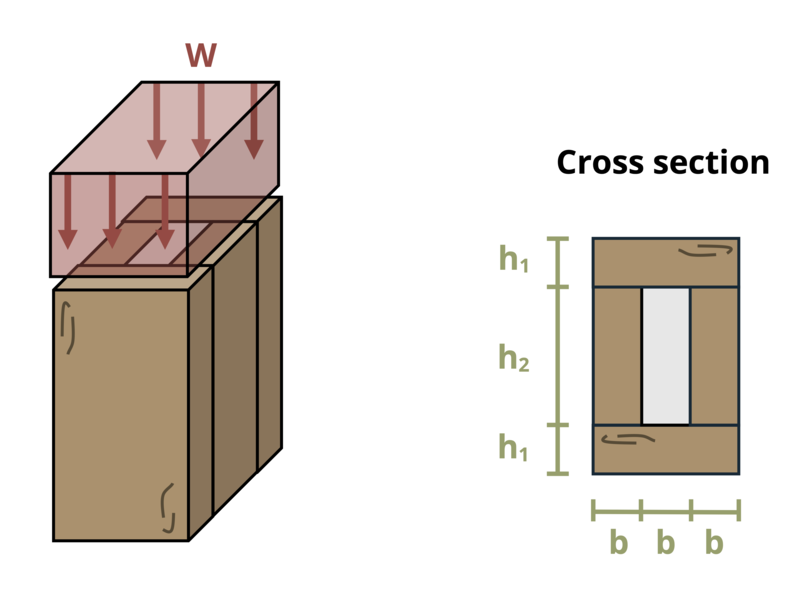
\includegraphics[keepaspectratio]{images/248.png}}
{[}Problem adapted from © Kurt Gramoll CC BY NC-SA 4.0{]}

\begin{Shaded}
\begin{Highlighting}[]
\NormalTok{\#| standalone: true}
\NormalTok{\#| viewerHeight: 600}
\NormalTok{\#| components: [viewer]}

\NormalTok{from shiny import App, render, ui, reactive}
\NormalTok{import random}
\NormalTok{import asyncio}
\NormalTok{import io}
\NormalTok{import math}
\NormalTok{import string}
\NormalTok{from datetime import datetime}
\NormalTok{from pathlib import Path}

\NormalTok{def generate\_random\_letters(length):}
\NormalTok{    \# Generate a random string of letters of specified length}
\NormalTok{    return \textquotesingle{}\textquotesingle{}.join(random.choice(string.ascii\_lowercase) for \_ in range(length)) }

\NormalTok{problem\_ID="248"}
\NormalTok{w=reactive.Value("\_\_")}
\NormalTok{b=reactive.Value("\_\_")}
\NormalTok{h1=reactive.Value("\_\_")}
\NormalTok{h2=reactive.Value("\_\_")}
\NormalTok{Econcrete=25}
\NormalTok{Ewood=12}

\NormalTok{attempts=["Timestamp,Attempt,Answer,Feedback\textbackslash{}n"]}

\NormalTok{app\_ui = ui.page\_fluid(}
\NormalTok{    \#ui.markdown("**Please enter your ID number from your instructor and click to generate your problem**"),}
\NormalTok{    \#ui.input\_text("ID","", placeholder="Enter ID Number Here"),}
\NormalTok{    \#ui.input\_action\_button("generate\_problem", "Generate Problem", class\_="btn{-}primary"),}
\NormalTok{    ui.markdown("**Problem Statement**"),}
\NormalTok{    ui.output\_ui("ui\_problem\_statement"),}
\NormalTok{    ui.input\_text("answer","Your Answer in units of kN", placeholder="Please enter your answer"),}
\NormalTok{    ui.input\_action\_button("submit", "Check Answer", class\_="btn{-}primary"),}
\NormalTok{    \#ui.download\_button("download", "Download File to Submit", class\_="btn{-}success"),}
\NormalTok{)}


\NormalTok{def server(input, output, session):}
\NormalTok{    \# Initialize a counter for attempts}
\NormalTok{    attempt\_counter = reactive.Value(0)}

\NormalTok{    @output}
\NormalTok{    @render.ui}
\NormalTok{    def ui\_problem\_statement():}
\NormalTok{        randomize\_vars()}
\NormalTok{        return[ui.markdown(f"A distributed load w = \{w()\} N/cm\textless{}sup\textgreater{}2\textless{}/sup\textgreater{} is applied to a short column made from wood and concrete. Assume E\textless{}sub\textgreater{}concrete \textless{}/sub\textgreater{}= 25 GPa, E\textless{}sub\textgreater{}wood\textless{}/sub\textgreater{} = 12 GPa, b = \{b()\} cm, h\textless{}sub\textgreater{}1\textless{}/sub\textgreater{} = \{h1()\} cm, and h\textless{}sub\textgreater{}2\textless{}/sub\textgreater{} = \{h2()\} cm. What load is carried by the concrete center?")]}
    
\NormalTok{    \#@reactive.Effect}
\NormalTok{    \#@reactive.event(input.generate\_problem)}
\NormalTok{    def randomize\_vars():}
\NormalTok{        random.seed(101)}
\NormalTok{        w.set(random.randrange(50, 750, 10))}
\NormalTok{        b.set(random.randrange(20, 100, 1)/10)}
\NormalTok{        h1.set(b()*1)}
\NormalTok{        h2.set(b()*2)}
        
\NormalTok{    @reactive.Effect}
\NormalTok{    @reactive.event(input.submit)}
\NormalTok{    def \_():}
\NormalTok{        attempt\_counter.set(attempt\_counter() + 1)  \# Increment the attempt counter on each submission.}
\NormalTok{        instr= (2.0833*h2()*w()*(2*h1()+h2())*3*b())/(6*h1()+4.0833*h2())/1000}
\NormalTok{        if math.isclose(float(input.answer()), instr, rel\_tol=0.01):}
\NormalTok{            check = "*Correct*"}
\NormalTok{            correct\_indicator = "JL"}
\NormalTok{        else:}
\NormalTok{            check = "*Not Correct.*"}
\NormalTok{            correct\_indicator = "JG"}

\NormalTok{        \# Generate random parts for the encoded attempt.}
\NormalTok{        random\_start = generate\_random\_letters(4)}
\NormalTok{        random\_middle = generate\_random\_letters(4)}
\NormalTok{        random\_end = generate\_random\_letters(4)}
\NormalTok{        \#encoded\_attempt = f"\{random\_start\}\{problem\_ID\}{-}\{random\_middle\}\{attempt\_counter()\}\{correct\_indicator\}{-}\{random\_end\}\{input.ID()\}"}

\NormalTok{        \# Store the most recent encoded attempt in a reactive value so it persists across submissions}
\NormalTok{        \#session.encoded\_attempt = reactive.Value(encoded\_attempt)}

\NormalTok{        \# Append the attempt data to the attempts list without the encoded attempt}
\NormalTok{        attempts.append(f"\{datetime.now()\}, \{attempt\_counter()\}, \{input.answer()\}, \{check\}\textbackslash{}n")}

\NormalTok{        \# Show feedback to the user.}
\NormalTok{        feedback = ui.markdown(f"Your answer of \{input.answer()\} is \{check\}.")}
\NormalTok{        m = ui.modal(}
\NormalTok{            feedback,}
\NormalTok{            title="Feedback",}
\NormalTok{            easy\_close=True}
\NormalTok{        )}
\NormalTok{        ui.modal\_show(m)}

\NormalTok{    \#@render.download(filename=lambda: f"Problem\_Log{-}\{problem\_ID\}{-}\{input.ID()\}.csv")}
\NormalTok{    async def download():}
\NormalTok{        \# Start the CSV with the encoded attempt (without label)}
\NormalTok{        final\_encoded = session.encoded\_attempt() if session.encoded\_attempt is not None else "No attempts"}
\NormalTok{        yield f"\{final\_encoded\}\textbackslash{}n\textbackslash{}n"}
        
\NormalTok{        \# Write the header for the remaining CSV data once}
\NormalTok{        yield "Timestamp,Attempt,Answer,Feedback\textbackslash{}n"}
        
\NormalTok{        \# Write the attempts data, ensure that the header from the attempts list is not written again}
\NormalTok{        for attempt in attempts[1:]:  \# Skip the first element which is the header}
\NormalTok{            await asyncio.sleep(0.25)  \# This delay may not be necessary; adjust as needed}
\NormalTok{            yield attempt}


\NormalTok{\# App installation}
\NormalTok{app = App(app\_ui, server)}
\end{Highlighting}
\end{Shaded}

\chapter*{Problem 5.39 - Statically Indeterminate Axial
Loads}\label{problem-5.39---statically-indeterminate-axial-loads}
\addcontentsline{toc}{chapter}{Problem 5.39 - Statically Indeterminate
Axial Loads}

\markboth{Problem 5.39 - Statically Indeterminate Axial Loads}{Problem
5.39 - Statically Indeterminate Axial Loads}

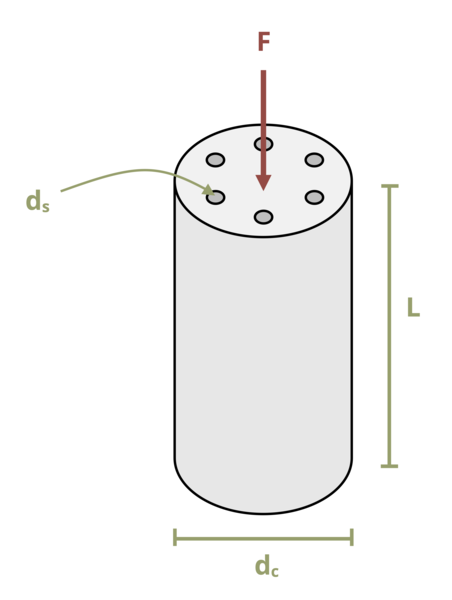
\includegraphics[width=2.60417in,height=\textheight,keepaspectratio]{images/250.png}
{[}Problem adapted from © Kurt Gramoll CC BY NC-SA 4.0{]}

\begin{Shaded}
\begin{Highlighting}[]
\NormalTok{\#| standalone: true}
\NormalTok{\#| viewerHeight: 600}
\NormalTok{\#| components: [viewer]}

\NormalTok{from shiny import App, render, ui, reactive}
\NormalTok{import random}
\NormalTok{import asyncio}
\NormalTok{import io}
\NormalTok{import math}
\NormalTok{import string}
\NormalTok{from datetime import datetime}
\NormalTok{from pathlib import Path}

\NormalTok{def generate\_random\_letters(length):}
\NormalTok{    \# Generate a random string of letters of specified length}
\NormalTok{    return \textquotesingle{}\textquotesingle{}.join(random.choice(string.ascii\_lowercase) for \_ in range(length)) }

\NormalTok{problem\_ID="250"}
\NormalTok{F=reactive.Value("\_\_")}
\NormalTok{L=reactive.Value("\_\_")}
\NormalTok{dc=reactive.Value("\_\_")}
\NormalTok{ds=reactive.Value("\_\_")}
\NormalTok{Econcrete=25}
\NormalTok{Esteel=200}

\NormalTok{attempts=["Timestamp,Attempt,Answer,Feedback\textbackslash{}n"]}

\NormalTok{app\_ui = ui.page\_fluid(}
\NormalTok{    \#ui.markdown("**Please enter your ID number from your instructor and click to generate your problem**"),}
\NormalTok{    \#ui.input\_text("ID","", placeholder="Enter ID Number Here"),}
\NormalTok{    \#ui.input\_action\_button("generate\_problem", "Generate Problem", class\_="btn{-}primary"),}
\NormalTok{    ui.markdown("**Problem Statement**"),}
\NormalTok{    ui.output\_ui("ui\_problem\_statement"),}
\NormalTok{    ui.input\_text("answer","Your Answer in units of MPa", placeholder="Please enter your answer"),}
\NormalTok{    ui.input\_action\_button("submit", "Check Answer", class\_="btn{-}primary"),}
\NormalTok{    \#ui.download\_button("download", "Download File to Submit", class\_="btn{-}success"),}
\NormalTok{)}


\NormalTok{def server(input, output, session):}
\NormalTok{    \# Initialize a counter for attempts}
\NormalTok{    attempt\_counter = reactive.Value(0)}

\NormalTok{    @output}
\NormalTok{    @render.ui}
\NormalTok{    def ui\_problem\_statement():}
\NormalTok{        randomize\_vars()}
\NormalTok{        return[ui.markdown(f"A concrete post of length L = \{L()\}  m and diameter d\textless{}sub\textgreater{}c\textless{}/sub\textgreater{} = \{dc()\} mm supports a load F = \{F()\} kN. The concrete is reinforced with 6 steel rods of diameter d\textless{}sub\textgreater{}s\textless{}/sub\textgreater{} = \{ds()\} mm. Assume E\textless{}sub\textgreater{}concrete\textless{}/sub\textgreater{} = 25 GPa and E\textless{}sub\textgreater{}steel\textless{}/sub\textgreater{} = 200 GPa. Determine the stress in the concrete.")]}
    
\NormalTok{    \#@reactive.Effect}
\NormalTok{    \#@reactive.event(input.generate\_problem)}
\NormalTok{    def randomize\_vars():}
\NormalTok{        random.seed(101)}
\NormalTok{        L.set(random.randrange(10, 50, 1)/10)}
\NormalTok{        dc.set(random.randrange(100, 500, 10))}
\NormalTok{        ds.set(round(dc()/12))}
\NormalTok{        F.set(random.randrange(100, 500, 10))}
        
\NormalTok{    @reactive.Effect}
\NormalTok{    @reactive.event(input.submit)}
\NormalTok{    def \_():}
\NormalTok{        attempt\_counter.set(attempt\_counter() + 1)  \# Increment the attempt counter on each submission.}
\NormalTok{        As = (math.pi*6*(ds()/20)**2)}
\NormalTok{        Ac = (math.pi*(dc()/20)**2) {-} As}
\NormalTok{        Cside = Ac*Econcrete}
\NormalTok{        Sside = As*Esteel}
\NormalTok{        LHS = F()*Cside}
\NormalTok{        RHS = Cside+Sside}
\NormalTok{        instr= ((LHS/RHS)/(Ac/100**2))/10**3}
\NormalTok{        if math.isclose(float(input.answer()), instr, rel\_tol=0.01):}
\NormalTok{            check = "*Correct*"}
\NormalTok{            correct\_indicator = "JL"}
\NormalTok{        else:}
\NormalTok{            check = "*Not Correct.*"}
\NormalTok{            correct\_indicator = "JG"}

\NormalTok{        \# Generate random parts for the encoded attempt.}
\NormalTok{        random\_start = generate\_random\_letters(4)}
\NormalTok{        random\_middle = generate\_random\_letters(4)}
\NormalTok{        random\_end = generate\_random\_letters(4)}
\NormalTok{        \#encoded\_attempt = f"\{random\_start\}\{problem\_ID\}{-}\{random\_middle\}\{attempt\_counter()\}\{correct\_indicator\}{-}\{random\_end\}\{input.ID()\}"}

\NormalTok{        \# Store the most recent encoded attempt in a reactive value so it persists across submissions}
\NormalTok{        \#session.encoded\_attempt = reactive.Value(encoded\_attempt)}

\NormalTok{        \# Append the attempt data to the attempts list without the encoded attempt}
\NormalTok{        attempts.append(f"\{datetime.now()\}, \{attempt\_counter()\}, \{input.answer()\}, \{check\}\textbackslash{}n")}

\NormalTok{        \# Show feedback to the user.}
\NormalTok{        feedback = ui.markdown(f"Your answer of \{input.answer()\} is \{check\}.")}
\NormalTok{        m = ui.modal(}
\NormalTok{            feedback,}
\NormalTok{            title="Feedback",}
\NormalTok{            easy\_close=True}
\NormalTok{        )}
\NormalTok{        ui.modal\_show(m)}

\NormalTok{    \#@render.download(filename=lambda: f"Problem\_Log{-}\{problem\_ID\}{-}\{input.ID()\}.csv")}
\NormalTok{    async def download():}
\NormalTok{        \# Start the CSV with the encoded attempt (without label)}
\NormalTok{        final\_encoded = session.encoded\_attempt() if session.encoded\_attempt is not None else "No attempts"}
\NormalTok{        yield f"\{final\_encoded\}\textbackslash{}n\textbackslash{}n"}
        
\NormalTok{        \# Write the header for the remaining CSV data once}
\NormalTok{        yield "Timestamp,Attempt,Answer,Feedback\textbackslash{}n"}
        
\NormalTok{        \# Write the attempts data, ensure that the header from the attempts list is not written again}
\NormalTok{        for attempt in attempts[1:]:  \# Skip the first element which is the header}
\NormalTok{            await asyncio.sleep(0.25)  \# This delay may not be necessary; adjust as needed}
\NormalTok{            yield attempt}


\NormalTok{\# App installation}
\NormalTok{app = App(app\_ui, server)}
\end{Highlighting}
\end{Shaded}

\chapter*{Problem 5.40 - Statically Indeterminate Axial
Loads}\label{problem-5.40---statically-indeterminate-axial-loads}
\addcontentsline{toc}{chapter}{Problem 5.40 - Statically Indeterminate
Axial Loads}

\markboth{Problem 5.40 - Statically Indeterminate Axial Loads}{Problem
5.40 - Statically Indeterminate Axial Loads}

\pandocbounded{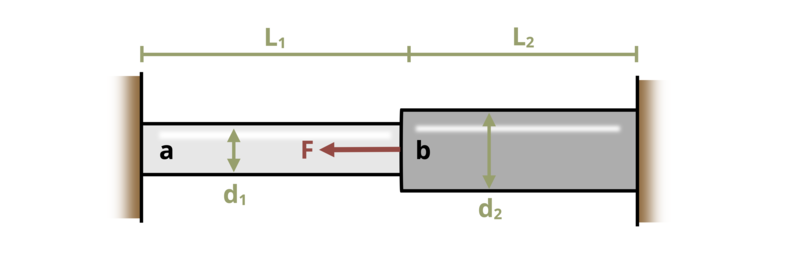
\includegraphics[keepaspectratio]{images/252.png}}
{[}Problem adapted from © Kurt Gramoll CC BY NC-SA 4.0{]}

\begin{Shaded}
\begin{Highlighting}[]
\NormalTok{\#| standalone: true}
\NormalTok{\#| viewerHeight: 600}
\NormalTok{\#| components: [viewer]}

\NormalTok{from shiny import App, render, ui, reactive}
\NormalTok{import random}
\NormalTok{import asyncio}
\NormalTok{import io}
\NormalTok{import math}
\NormalTok{import string}
\NormalTok{from datetime import datetime}
\NormalTok{from pathlib import Path}

\NormalTok{def generate\_random\_letters(length):}
\NormalTok{    \# Generate a random string of letters of specified length}
\NormalTok{    return \textquotesingle{}\textquotesingle{}.join(random.choice(string.ascii\_lowercase) for \_ in range(length))}

\NormalTok{problem\_ID="252"}
\NormalTok{L2=reactive.Value("\_\_")}
\NormalTok{L1=reactive.Value("\_\_")}
\NormalTok{d1=reactive.Value("\_\_")}
\NormalTok{d2=reactive.Value("\_\_")}
\NormalTok{F=reactive.Value("\_\_")}

\NormalTok{attempts=["Timestamp,Attempt,Answer,Feedback\textbackslash{}n"]}

\NormalTok{app\_ui = ui.page\_fluid(}
\NormalTok{    \#ui.markdown("**Please enter your ID number from your instructor and click to generate your problem**"),}
\NormalTok{    \#ui.input\_text("ID","", placeholder="Enter ID Number Here"),}
\NormalTok{    \#ui.input\_action\_button("generate\_problem", "Generate Problem", class\_="btn{-}primary"),}
\NormalTok{    ui.markdown("**Problem Statement**"),}
\NormalTok{    ui.output\_ui("ui\_problem\_statement"),}
\NormalTok{    ui.input\_text("answer","Your Answer in units of MPa", placeholder="Please enter your answer"),}
\NormalTok{    ui.input\_action\_button("submit", "Check Answer", class\_="btn{-}primary"),}
\NormalTok{    \#ui.download\_button("download", "Download File to Submit", class\_="btn{-}success"),}
\NormalTok{)}

\NormalTok{def server(input, output, session):}
\NormalTok{    \# Initialize a counter for attempts}
\NormalTok{    attempt\_counter = reactive.Value(0)}

\NormalTok{    @output}
\NormalTok{    @render.ui}
\NormalTok{    def ui\_problem\_statement():}
\NormalTok{        randomize\_vars()}
\NormalTok{        return[ui.markdown(f"Two circular rods are attached together and fixed between two walls. Length L\textless{}sub\textgreater{}1\textless{}/sub\textgreater{} = \{L1()\} m, L\textless{}sub\textgreater{}2\textless{}/sub\textgreater{} = \{L2()\} m, diameter d\textless{}sub\textgreater{}1\textless{}/sub\textgreater{} = \{d1()\} mm, and d\textless{}sub\textgreater{}2\textless{}/sub\textgreater{} = \{d2()\} mm. A force F = \{F()\} kN is applied as shown. Determine the largest stress in either rod. Assume E = 190 GPa.")]}
    
\NormalTok{    \#@reactive.Effect}
\NormalTok{    \#@reactive.event(input.generate\_problem)}
\NormalTok{    def randomize\_vars():}
\NormalTok{        random.seed(101)}
\NormalTok{        L2.set(random.randrange(20,80,5)/100)}
\NormalTok{        L1.set(round(L2())+(random.randrange(5,20,5)/100))}
\NormalTok{        d1.set(random.randrange(20,50,1))}
\NormalTok{        d2.set(d1()+random.randrange(5,15,1))}
\NormalTok{        F.set(random.randrange(10,100,1))}
        
\NormalTok{    @reactive.Effect}
\NormalTok{    @reactive.event(input.submit)}
\NormalTok{    def \_():}
\NormalTok{        attempt\_counter.set(attempt\_counter() + 1)  \# Increment the attempt counter on each submission.}
\NormalTok{        Fa = F()*L2()/((d2()/2000)**2*math.pi)/(L1()/((d1()/2000)**2*math.pi)+L2()/((d2()/2000)**2*math.pi))}
\NormalTok{        Fb = F(){-}Fa}
\NormalTok{        sigmaA = Fa/((d1()/2000)**2*math.pi)/1000}
\NormalTok{        sigmaB = Fb/((d2()/2000)**2*math.pi)/1000}
\NormalTok{        instr = max(sigmaA,sigmaB)}
\NormalTok{        if math.isclose(float(input.answer()), instr, rel\_tol=0.01):}
\NormalTok{            check = "*Correct*"}
\NormalTok{            correct\_indicator = "JL"}
\NormalTok{        else:}
\NormalTok{            check = "*Not Correct.*"}
\NormalTok{            correct\_indicator = "JG"}

\NormalTok{        \# Generate random parts for the encoded attempt.}
\NormalTok{        random\_start = generate\_random\_letters(4)}
\NormalTok{        random\_middle = generate\_random\_letters(4)}
\NormalTok{        random\_end = generate\_random\_letters(4)}
\NormalTok{        \#encoded\_attempt = f"\{random\_start\}\{problem\_ID\}{-}\{random\_middle\}\{attempt\_counter()\}\{correct\_indicator\}{-}\{random\_end\}\{input.ID()\}"}

\NormalTok{        \# Store the most recent encoded attempt in a reactive value so it persists across submissions}
\NormalTok{        \#session.encoded\_attempt = reactive.Value(encoded\_attempt)}

\NormalTok{        \# Append the attempt data to the attempts list without the encoded attempt}
\NormalTok{        attempts.append(f"\{datetime.now()\}, \{attempt\_counter()\}, \{input.answer()\}, \{check\}\textbackslash{}n")}

\NormalTok{        \# Show feedback to the user.}
\NormalTok{        feedback = ui.markdown(f"Your answer of \{input.answer()\} is \{check\}.")}
\NormalTok{        m = ui.modal(}
\NormalTok{            feedback,}
\NormalTok{            title="Feedback",}
\NormalTok{            easy\_close=True}
\NormalTok{        )}
\NormalTok{        ui.modal\_show(m)}

\NormalTok{    \#@render.download(filename=lambda: f"Problem\_Log{-}\{problem\_ID\}{-}\{input.ID()\}.csv")}
\NormalTok{    async def download():}
\NormalTok{        \# Start the CSV with the encoded attempt (without label)}
\NormalTok{        final\_encoded = session.encoded\_attempt() if session.encoded\_attempt is not None else "No attempts"}
\NormalTok{        yield f"\{final\_encoded\}\textbackslash{}n\textbackslash{}n"}
        
\NormalTok{        \# Write the header for the remaining CSV data once}
\NormalTok{        yield "Timestamp,Attempt,Answer,Feedback\textbackslash{}n"}
        
\NormalTok{        \# Write the attempts data, ensure that the header from the attempts list is not written again}
\NormalTok{        for attempt in attempts[1:]:  \# Skip the first element which is the header}
\NormalTok{            await asyncio.sleep(0.25)  \# This delay may not be necessary; adjust as needed}
\NormalTok{            yield attempt}

\NormalTok{\# App installation}
\NormalTok{app = App(app\_ui, server)}
\end{Highlighting}
\end{Shaded}

\chapter*{Problem 5.41 - Statically Indeterminate Axial
Loads}\label{problem-5.41---statically-indeterminate-axial-loads}
\addcontentsline{toc}{chapter}{Problem 5.41 - Statically Indeterminate
Axial Loads}

\markboth{Problem 5.41 - Statically Indeterminate Axial Loads}{Problem
5.41 - Statically Indeterminate Axial Loads}

\pandocbounded{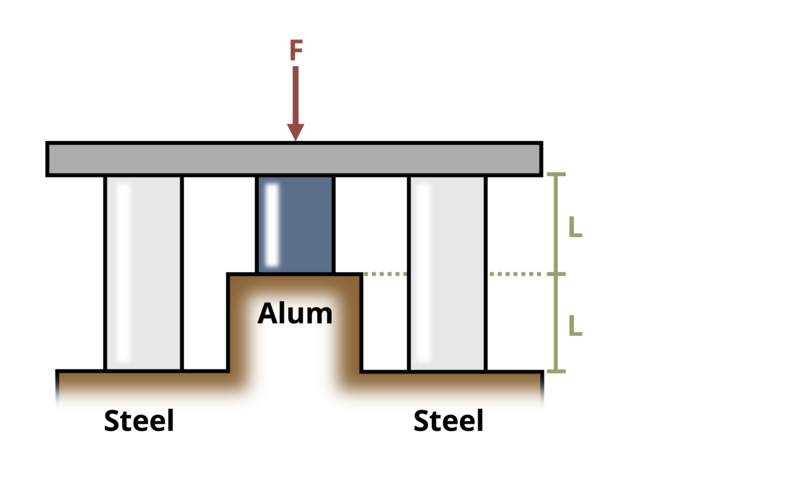
\includegraphics[keepaspectratio]{images/254.png}}
{[}Problem adapted from © Kurt Gramoll CC BY NC-SA 4.0{]}

\begin{Shaded}
\begin{Highlighting}[]
\NormalTok{\#| standalone: true}
\NormalTok{\#| viewerHeight: 600}
\NormalTok{\#| components: [viewer]}

\NormalTok{from shiny import App, render, ui, reactive}
\NormalTok{import random}
\NormalTok{import asyncio}
\NormalTok{import io}
\NormalTok{import math}
\NormalTok{import string}
\NormalTok{from datetime import datetime}
\NormalTok{from pathlib import Path}

\NormalTok{def generate\_random\_letters(length):}
\NormalTok{    \# Generate a random string of letters of specified length}
\NormalTok{    return \textquotesingle{}\textquotesingle{}.join(random.choice(string.ascii\_lowercase) for \_ in range(length))}

\NormalTok{problem\_ID="254"}
\NormalTok{F=reactive.Value("\_\_")}
\NormalTok{L=reactive.Value("\_\_")}
\NormalTok{d=reactive.Value("\_\_")}

\NormalTok{attempts=["Timestamp,Attempt,Answer,Feedback\textbackslash{}n"]}

\NormalTok{app\_ui = ui.page\_fluid(}
\NormalTok{    \#ui.markdown("**Please enter your ID number from your instructor and click to generate your problem**"),}
\NormalTok{    \#ui.input\_text("ID","", placeholder="Enter ID Number Here"),}
\NormalTok{    \#ui.input\_action\_button("generate\_problem", "Generate Problem", class\_="btn{-}primary"),}
\NormalTok{    ui.markdown("**Problem Statement**"),}
\NormalTok{    ui.output\_ui("ui\_problem\_statement"),}
\NormalTok{    ui.input\_text("answer","Your Answer in units of MPa", placeholder="Please enter your answer"),}
\NormalTok{    ui.input\_action\_button("submit", "Check Answer", class\_="btn{-}primary"),}
\NormalTok{    \#ui.download\_button("download", "Download File to Submit", class\_="btn{-}success"),}
\NormalTok{)}

\NormalTok{def server(input, output, session):}
\NormalTok{    \# Initialize a counter for attempts}
\NormalTok{    attempt\_counter = reactive.Value(0)}

\NormalTok{    @output}
\NormalTok{    @render.ui}
\NormalTok{    def ui\_problem\_statement():}
\NormalTok{        randomize\_vars()}
\NormalTok{        return[ui.markdown(f"Three cylinders support a load F = \{F()\} kN. If length L = \{L()\} m, determine the stress in the aluminum cylinder. Assume E\textless{}sub\textgreater{}steel\textless{}/sub\textgreater{} = 200 GPA, E\textless{}sub\textgreater{}alum\textless{}/sub\textgreater{} = 70 GPA, and the diameter of each cylinder d = \{d()\} mm.")]}
    
\NormalTok{    \#@reactive.Effect}
\NormalTok{    \#@reactive.event(input.generate\_problem)}
\NormalTok{    def randomize\_vars():}
\NormalTok{        random.seed(101)}
\NormalTok{        F.set(random.randrange(100,500,10))}
\NormalTok{        L.set(random.randrange(5,50,1)/10)}
\NormalTok{        d.set(random.randrange(25,100,1))}
                
\NormalTok{    @reactive.Effect}
\NormalTok{    @reactive.event(input.submit)}
\NormalTok{    def \_():}
\NormalTok{        attempt\_counter.set(attempt\_counter() + 1)  \# Increment the attempt counter on each submission.}
\NormalTok{        FB = F()/((2*L()*200)/(2*L()*70)+1)}
\NormalTok{        instr = FB/(math.pi*(d()/2000)**2)}
\NormalTok{        if math.isclose(float(input.answer()), instr, rel\_tol=0.01):}
\NormalTok{            check = "*Correct*"}
\NormalTok{            correct\_indicator = "JL"}
\NormalTok{        else:}
\NormalTok{            check = "*Not Correct.*"}
\NormalTok{            correct\_indicator = "JG"}

\NormalTok{        \# Generate random parts for the encoded attempt.}
\NormalTok{        random\_start = generate\_random\_letters(4)}
\NormalTok{        random\_middle = generate\_random\_letters(4)}
\NormalTok{        random\_end = generate\_random\_letters(4)}
\NormalTok{        \#encoded\_attempt = f"\{random\_start\}\{problem\_ID\}{-}\{random\_middle\}\{attempt\_counter()\}\{correct\_indicator\}{-}\{random\_end\}\{input.ID()\}"}

\NormalTok{        \# Store the most recent encoded attempt in a reactive value so it persists across submissions}
\NormalTok{        \#session.encoded\_attempt = reactive.Value(encoded\_attempt)}

\NormalTok{        \# Append the attempt data to the attempts list without the encoded attempt}
\NormalTok{        attempts.append(f"\{datetime.now()\}, \{attempt\_counter()\}, \{input.answer()\}, \{check\}\textbackslash{}n")}

\NormalTok{        \# Show feedback to the user.}
\NormalTok{        feedback = ui.markdown(f"Your answer of \{input.answer()\} is \{check\}.")}
\NormalTok{        m = ui.modal(}
\NormalTok{            feedback,}
\NormalTok{            title="Feedback",}
\NormalTok{            easy\_close=True}
\NormalTok{        )}
\NormalTok{        ui.modal\_show(m)}

\NormalTok{    \#@render.download(filename=lambda: f"Problem\_Log{-}\{problem\_ID\}{-}\{input.ID()\}.csv")}
\NormalTok{    async def download():}
\NormalTok{        \# Start the CSV with the encoded attempt (without label)}
\NormalTok{        final\_encoded = session.encoded\_attempt() if session.encoded\_attempt is not None else "No attempts"}
\NormalTok{        yield f"\{final\_encoded\}\textbackslash{}n\textbackslash{}n"}
        
\NormalTok{        \# Write the header for the remaining CSV data once}
\NormalTok{        yield "Timestamp,Attempt,Answer,Feedback\textbackslash{}n"}
        
\NormalTok{        \# Write the attempts data, ensure that the header from the attempts list is not written again}
\NormalTok{        for attempt in attempts[1:]:  \# Skip the first element which is the header}
\NormalTok{            await asyncio.sleep(0.25)  \# This delay may not be necessary; adjust as needed}
\NormalTok{            yield attempt}

\NormalTok{\# App installation}
\NormalTok{app = App(app\_ui, server)}
\end{Highlighting}
\end{Shaded}

\chapter*{Problem 5.42 - Statically Indeterminate Axial
Loads}\label{problem-5.42---statically-indeterminate-axial-loads}
\addcontentsline{toc}{chapter}{Problem 5.42 - Statically Indeterminate
Axial Loads}

\markboth{Problem 5.42 - Statically Indeterminate Axial Loads}{Problem
5.42 - Statically Indeterminate Axial Loads}

\pandocbounded{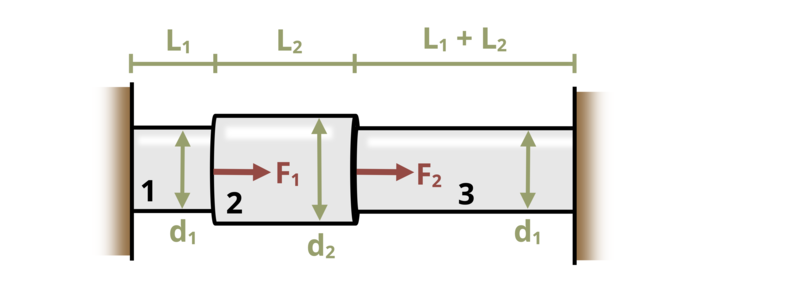
\includegraphics[keepaspectratio]{images/255.png}}
{[}Problem adapted from © Kurt Gramoll CC BY NC-SA 4.0{]}

\begin{Shaded}
\begin{Highlighting}[]
\NormalTok{\#| standalone: true}
\NormalTok{\#| viewerHeight: 600}
\NormalTok{\#| components: [viewer]}

\NormalTok{from shiny import App, render, ui, reactive}
\NormalTok{import random}
\NormalTok{import asyncio}
\NormalTok{import io}
\NormalTok{import math}
\NormalTok{import string}
\NormalTok{from datetime import datetime}
\NormalTok{from pathlib import Path}

\NormalTok{def generate\_random\_letters(length):}
\NormalTok{    \# Generate a random string of letters of specified length}
\NormalTok{    return \textquotesingle{}\textquotesingle{}.join(random.choice(string.ascii\_lowercase) for \_ in range(length))}

\NormalTok{problem\_ID="255"}
\NormalTok{F1=reactive.Value("\_\_")}
\NormalTok{F2=reactive.Value("\_\_")}

\NormalTok{attempts=["Timestamp,Attempt,Answer,Feedback\textbackslash{}n"]}

\NormalTok{app\_ui = ui.page\_fluid(}
\NormalTok{    \#ui.markdown("**Please enter your ID number from your instructor and click to generate your problem**"),}
\NormalTok{    \#ui.input\_text("ID","", placeholder="Enter ID Number Here"),}
\NormalTok{    \#ui.input\_action\_button("generate\_problem", "Generate Problem", class\_="btn{-}primary"),}
\NormalTok{    ui.markdown("**Problem Statement**"),}
\NormalTok{    ui.output\_ui("ui\_problem\_statement"),}
\NormalTok{    ui.input\_text("answer","Your Answer in units of psi", placeholder="Please enter your answer"),}
\NormalTok{    ui.input\_action\_button("submit", "Check Answer", class\_="btn{-}primary"),}
\NormalTok{    \#ui.download\_button("download", "Download File to Submit", class\_="btn{-}success"),}
\NormalTok{)}

\NormalTok{def server(input, output, session):}
\NormalTok{    \# Initialize a counter for attempts}
\NormalTok{    attempt\_counter = reactive.Value(0)}

\NormalTok{    @output}
\NormalTok{    @render.ui}
\NormalTok{    def ui\_problem\_statement():}
\NormalTok{        randomize\_vars()}
\NormalTok{        return[ui.markdown(f"Three circular steel rods (E = 29,000 ksi) are placed between two fixed walls as shown. Loads F\textless{}sub\textgreater{}1\textless{}/sub\textgreater{} = \{F1()\} kips and F\textless{}sub\textgreater{}2\textless{}/sub\textgreater{} = \{F2()\} kips are applied to the assembly. Determine the average normal stress in member 3. Please submit a positive answer for tension or a negative answer for compression.")]}
    
\NormalTok{    \#@reactive.Effect}
\NormalTok{    \#@reactive.event(input.generate\_problem)}
\NormalTok{    def randomize\_vars():}
\NormalTok{        random.seed(101)}
\NormalTok{        F1.set(random.randrange(10,50,1))}
\NormalTok{        F2.set(random.randrange(10,50,1))}
                
\NormalTok{    @reactive.Effect}
\NormalTok{    @reactive.event(input.submit)}
\NormalTok{    def \_():}
\NormalTok{        attempt\_counter.set(attempt\_counter() + 1)  \# Increment the attempt counter on each submission.}
\NormalTok{        A1 = math.pi*0.5**2}
\NormalTok{        A2 = math.pi*0.75**2}
\NormalTok{        A3 = A1}
\NormalTok{        L1 = 1}
\NormalTok{        L2 = 2}
\NormalTok{        L3 = 3}
\NormalTok{        FA = (F1()*L2/A2+F1()*L3/A3+F2()*L3/A3)/(L1/A1+L2/A2+L3/A3)}
\NormalTok{        FR3 = FA{-}F1(){-}F2()}
\NormalTok{        instr = FR3*1000/A3}
\NormalTok{        if math.isclose(float(input.answer()), instr, rel\_tol=0.01):}
\NormalTok{            check = "*Correct*"}
\NormalTok{            correct\_indicator = "JL"}
\NormalTok{        else:}
\NormalTok{            check = "*Not Correct.*"}
\NormalTok{            correct\_indicator = "JG"}

\NormalTok{        \# Generate random parts for the encoded attempt.}
\NormalTok{        random\_start = generate\_random\_letters(4)}
\NormalTok{        random\_middle = generate\_random\_letters(4)}
\NormalTok{        random\_end = generate\_random\_letters(4)}
\NormalTok{        \#encoded\_attempt = f"\{random\_start\}\{problem\_ID\}{-}\{random\_middle\}\{attempt\_counter()\}\{correct\_indicator\}{-}\{random\_end\}\{input.ID()\}"}

\NormalTok{        \# Store the most recent encoded attempt in a reactive value so it persists across submissions}
\NormalTok{        \#session.encoded\_attempt = reactive.Value(encoded\_attempt)}

\NormalTok{        \# Append the attempt data to the attempts list without the encoded attempt}
\NormalTok{        attempts.append(f"\{datetime.now()\}, \{attempt\_counter()\}, \{input.answer()\}, \{check\}\textbackslash{}n")}

\NormalTok{        \# Show feedback to the user.}
\NormalTok{        feedback = ui.markdown(f"Your answer of \{input.answer()\} is \{check\}.")}
\NormalTok{        m = ui.modal(}
\NormalTok{            feedback,}
\NormalTok{            title="Feedback",}
\NormalTok{            easy\_close=True}
\NormalTok{        )}
\NormalTok{        ui.modal\_show(m)}

\NormalTok{    \#@render.download(filename=lambda: f"Problem\_Log{-}\{problem\_ID\}{-}\{input.ID()\}.csv")}
\NormalTok{    async def download():}
\NormalTok{        \# Start the CSV with the encoded attempt (without label)}
\NormalTok{        final\_encoded = session.encoded\_attempt() if session.encoded\_attempt is not None else "No attempts"}
\NormalTok{        yield f"\{final\_encoded\}\textbackslash{}n\textbackslash{}n"}
        
\NormalTok{        \# Write the header for the remaining CSV data once}
\NormalTok{        yield "Timestamp,Attempt,Answer,Feedback\textbackslash{}n"}
        
\NormalTok{        \# Write the attempts data, ensure that the header from the attempts list is not written again}
\NormalTok{        for attempt in attempts[1:]:  \# Skip the first element which is the header}
\NormalTok{            await asyncio.sleep(0.25)  \# This delay may not be necessary; adjust as needed}
\NormalTok{            yield attempt}

\NormalTok{\# App installation}
\NormalTok{app = App(app\_ui, server)}
\end{Highlighting}
\end{Shaded}

\chapter*{Problem 5.43 - Statically Indeterminate Axial
Loads}\label{problem-5.43---statically-indeterminate-axial-loads}
\addcontentsline{toc}{chapter}{Problem 5.43 - Statically Indeterminate
Axial Loads}

\markboth{Problem 5.43 - Statically Indeterminate Axial Loads}{Problem
5.43 - Statically Indeterminate Axial Loads}

\pandocbounded{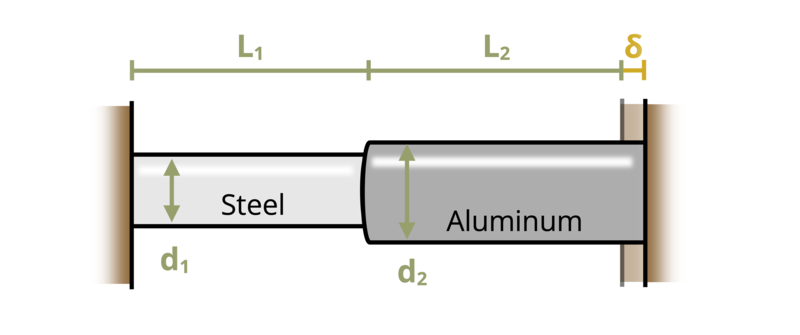
\includegraphics[keepaspectratio]{images/261.png}}
{[}Problem adapted from © Kurt Gramoll CC BY NC-SA 4.0{]}

\begin{Shaded}
\begin{Highlighting}[]
\NormalTok{\#| standalone: true}
\NormalTok{\#| viewerHeight: 600}
\NormalTok{\#| components: [viewer]}

\NormalTok{from shiny import App, render, ui, reactive}
\NormalTok{import random}
\NormalTok{import asyncio}
\NormalTok{import io}
\NormalTok{import math}
\NormalTok{import string}
\NormalTok{from datetime import datetime}
\NormalTok{from pathlib import Path}

\NormalTok{def generate\_random\_letters(length):}
\NormalTok{    \# Generate a random string of letters of specified length}
\NormalTok{    return \textquotesingle{}\textquotesingle{}.join(random.choice(string.ascii\_lowercase) for \_ in range(length))}

\NormalTok{problem\_ID="261"}
\NormalTok{delta=reactive.Value("\_\_")}
\NormalTok{L1=reactive.Value("\_\_")}
\NormalTok{L2=reactive.Value("\_\_")}
\NormalTok{r1=reactive.Value("\_\_")}
\NormalTok{r2=reactive.Value("\_\_")}

\NormalTok{attempts=["Timestamp,Attempt,Answer,Feedback\textbackslash{}n"]}

\NormalTok{app\_ui = ui.page\_fluid(}
\NormalTok{    \#ui.markdown("**Please enter your ID number from your instructor and click to generate your problem**"),}
\NormalTok{    \#ui.input\_text("ID","", placeholder="Enter ID Number Here"),}
\NormalTok{    \#ui.input\_action\_button("generate\_problem", "Generate Problem", class\_="btn{-}primary"),}
\NormalTok{    ui.markdown("**Problem Statement**"),}
\NormalTok{    ui.output\_ui("ui\_problem\_statement"),}
\NormalTok{    ui.input\_text("answer","Your Answer in units of kip", placeholder="Please enter your answer"),}
\NormalTok{    ui.input\_action\_button("submit", "Check Answer", class\_="btn{-}primary"),}
\NormalTok{    \#ui.download\_button("download", "Download File to Submit", class\_="btn{-}success"),}
\NormalTok{)}

\NormalTok{def server(input, output, session):}
\NormalTok{    \# Initialize a counter for attempts}
\NormalTok{    attempt\_counter = reactive.Value(0)}

\NormalTok{    @output}
\NormalTok{    @render.ui}
\NormalTok{    def ui\_problem\_statement():}
\NormalTok{        randomize\_vars()}
\NormalTok{        return[ui.markdown(f"Two circular rods are attached together and placed between two fixed surfaces. The right surface is moved to the right by ẟ = \{delta()\} in., stretching the two rods. Determine the force at the right wall. Assume E\textless{}sub\textgreater{}steel\textless{}/sub\textgreater{} = 29,000 ksi, E\textless{}sub\textgreater{}alum\textless{}/sub\textgreater{} = 10,000 ksi, L\textless{}sub\textgreater{}1\textless{}/sub\textgreater{} = \{L1()\} in., L\textless{}sub\textgreater{}2\textless{}/sub\textgreater{} = \{L2()\} in., r\textless{}sub\textgreater{}1\textless{}/sub\textgreater{} = \{r1()\} in., and r\textless{}sub\textgreater{}2\textless{}/sub\textgreater{} = \{r2()\} in.")]}
    
\NormalTok{    \#@reactive.Effect}
\NormalTok{    \#@reactive.event(input.generate\_problem)}
\NormalTok{    def randomize\_vars():}
\NormalTok{        random.seed(101)}
\NormalTok{        delta.set(random.randrange(1,5,1)/100)}
\NormalTok{        L1.set(random.randrange(5,20,1))}
\NormalTok{        L2.set(round(L1()*1.3,1))}
\NormalTok{        r1.set(random.randrange(20,200,5)/100)}
\NormalTok{        r2.set(round(r1()*1.5,1))}
    
\NormalTok{    @reactive.Effect}
\NormalTok{    @reactive.event(input.submit)}
\NormalTok{    def \_():}
\NormalTok{        attempt\_counter.set(attempt\_counter() + 1)  \# Increment the attempt counter on each submission.}
        
\NormalTok{        instr = delta()/(L1()/(29*10**6*r1()**2*math.pi)+L2()/(10*10**6*math.pi*r2()**2))/1000}
\NormalTok{        if math.isclose(float(input.answer()), instr, rel\_tol=0.01):}
\NormalTok{            check = "*Correct*"}
\NormalTok{            correct\_indicator = "JL"}
\NormalTok{        else:}
\NormalTok{            check = "*Not Correct.*"}
\NormalTok{            correct\_indicator = "JG"}

\NormalTok{        \# Generate random parts for the encoded attempt.}
\NormalTok{        random\_start = generate\_random\_letters(4)}
\NormalTok{        random\_middle = generate\_random\_letters(4)}
\NormalTok{        random\_end = generate\_random\_letters(4)}
\NormalTok{        \#encoded\_attempt = f"\{random\_start\}\{problem\_ID\}{-}\{random\_middle\}\{attempt\_counter()\}\{correct\_indicator\}{-}\{random\_end\}\{input.ID()\}"}

\NormalTok{        \# Store the most recent encoded attempt in a reactive value so it persists across submissions}
\NormalTok{        \#session.encoded\_attempt = reactive.Value(encoded\_attempt)}

\NormalTok{        \# Append the attempt data to the attempts list without the encoded attempt}
\NormalTok{        attempts.append(f"\{datetime.now()\}, \{attempt\_counter()\}, \{input.answer()\}, \{check\}\textbackslash{}n")}

\NormalTok{        \# Show feedback to the user.}
\NormalTok{        feedback = ui.markdown(f"Your answer of \{input.answer()\} is \{check\}.")}
\NormalTok{        m = ui.modal(}
\NormalTok{            feedback,}
\NormalTok{            title="Feedback",}
\NormalTok{            easy\_close=True}
\NormalTok{        )}
\NormalTok{        ui.modal\_show(m)}

\NormalTok{    \#@render.download(filename=lambda: f"Problem\_Log{-}\{problem\_ID\}{-}\{input.ID()\}.csv")}
\NormalTok{    async def download():}
\NormalTok{        \# Start the CSV with the encoded attempt (without label)}
\NormalTok{        final\_encoded = session.encoded\_attempt() if session.encoded\_attempt is not None else "No attempts"}
\NormalTok{        yield f"\{final\_encoded\}\textbackslash{}n\textbackslash{}n"}
        
\NormalTok{        \# Write the header for the remaining CSV data once}
\NormalTok{        yield "Timestamp,Attempt,Answer,Feedback\textbackslash{}n"}
        
\NormalTok{        \# Write the attempts data, ensure that the header from the attempts list is not written again}
\NormalTok{        for attempt in attempts[1:]:  \# Skip the first element which is the header}
\NormalTok{            await asyncio.sleep(0.25)  \# This delay may not be necessary; adjust as needed}
\NormalTok{            yield attempt}

\NormalTok{\# App installation}
\NormalTok{app = App(app\_ui, server)}
\end{Highlighting}
\end{Shaded}

\chapter*{Problem 5.44 - Statically Indeterminate Axial
Loads}\label{problem-5.44---statically-indeterminate-axial-loads}
\addcontentsline{toc}{chapter}{Problem 5.44 - Statically Indeterminate
Axial Loads}

\markboth{Problem 5.44 - Statically Indeterminate Axial Loads}{Problem
5.44 - Statically Indeterminate Axial Loads}

\pandocbounded{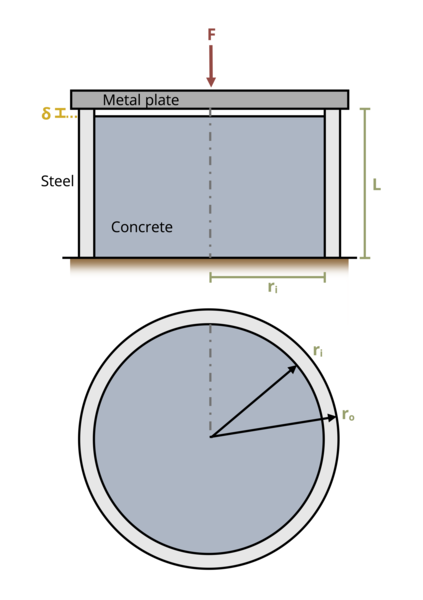
\includegraphics[keepaspectratio]{images/262.png}}
{[}Problem adapted from © Kurt Gramoll CC BY NC-SA 4.0{]}

\begin{Shaded}
\begin{Highlighting}[]
\NormalTok{\#| standalone: true}
\NormalTok{\#| viewerHeight: 600}
\NormalTok{\#| components: [viewer]}

\NormalTok{from shiny import App, render, ui, reactive}
\NormalTok{import random}
\NormalTok{import asyncio}
\NormalTok{import io}
\NormalTok{import math}
\NormalTok{import string}
\NormalTok{from datetime import datetime}
\NormalTok{from pathlib import Path}

\NormalTok{def generate\_random\_letters(length):}
\NormalTok{    \# Generate a random string of letters of specified length}
\NormalTok{    return \textquotesingle{}\textquotesingle{}.join(random.choice(string.ascii\_lowercase) for \_ in range(length))}

\NormalTok{problem\_ID="262"}
\NormalTok{ri=reactive.Value("\_\_")}
\NormalTok{ro=reactive.Value("\_\_")}
\NormalTok{L=reactive.Value("\_\_")}
\NormalTok{delta=reactive.Value("\_\_")}
\NormalTok{F=reactive.Value("\_\_")}

\NormalTok{attempts=["Timestamp,Attempt,Answer,Feedback\textbackslash{}n"]}

\NormalTok{app\_ui = ui.page\_fluid(}
\NormalTok{    \#ui.markdown("**Please enter your ID number from your instructor and click to generate your problem**"),}
\NormalTok{    \#ui.input\_text("ID","", placeholder="Enter ID Number Here"),}
\NormalTok{    \#ui.input\_action\_button("generate\_problem", "Generate Problem", class\_="btn{-}primary"),}
\NormalTok{    ui.markdown("**Problem Statement**"),}
\NormalTok{    ui.output\_ui("ui\_problem\_statement"),}
\NormalTok{    ui.input\_text("answer","Your Answer in units of ksi", placeholder="Please enter your answer"),}
\NormalTok{    ui.input\_action\_button("submit", "Check Answer", class\_="btn{-}primary"),}
\NormalTok{    \#ui.download\_button("download", "Download File to Submit", class\_="btn{-}success"),}
\NormalTok{)}

\NormalTok{def server(input, output, session):}
\NormalTok{    \# Initialize a counter for attempts}
\NormalTok{    attempt\_counter = reactive.Value(0)}

\NormalTok{    @output}
\NormalTok{    @render.ui}
\NormalTok{    def ui\_problem\_statement():}
\NormalTok{        randomize\_vars()}
\NormalTok{        return[ui.markdown(f"A steel tube of inner radius r\textless{}sub\textgreater{}i\textless{}/sub\textgreater{} = \{ri()\} in., outer radius r\textless{}sub\textgreater{}o\textless{}/sub\textgreater{} = \{ro()\} in., and length L = \{L()\} in. is filled with concrete except for a small gap at the top of ẟ = \{delta()\} in. A rigid metal plate is loaded with force F = \{F()\} kips. Determine the stress in the steel tube. Assume E\textless{}sub\textgreater{}c\textless{}/sub\textgreater{} = 4,000 ksi and E\textless{}sub\textgreater{}s\textless{}/sub\textgreater{} = 29,000 ksi.")]}
    
\NormalTok{    \#@reactive.Effect}
\NormalTok{    \#@reactive.event(input.generate\_problem)}
\NormalTok{    def randomize\_vars():}
\NormalTok{        random.seed(101)}
\NormalTok{        ri.set(random.randrange(25,50,1)/10)}
\NormalTok{        ro.set(round(ri())+random.randrange(1,5,1)/10)}
\NormalTok{        L.set(random.randrange(30,60,1))}
\NormalTok{        delta.set(random.randrange(1,5,1)/1000)}
\NormalTok{        F.set(random.randrange(100,300,10))}
    
\NormalTok{    @reactive.Effect}
\NormalTok{    @reactive.event(input.submit)}
\NormalTok{    def \_():}
\NormalTok{        attempt\_counter.set(attempt\_counter() + 1)  \# Increment the attempt counter on each submission.}
\NormalTok{        As = (ro()**2{-}ri()**2)*math.pi}
\NormalTok{        Ac = ri()**2*math.pi}
\NormalTok{        Ec = 4000}
\NormalTok{        Es = 29000}
\NormalTok{        Lc = L(){-}delta()}
\NormalTok{        Fc = (F()*L()/(As*Es){-}delta())/(Lc/(Ac*Ec)+L()/(As*Es))}
\NormalTok{        Fs = F(){-}Fc}
\NormalTok{        instr = Fs/As}
\NormalTok{        if math.isclose(float(input.answer()), instr, rel\_tol=0.01):}
\NormalTok{            check = "*Correct*"}
\NormalTok{            correct\_indicator = "JL"}
\NormalTok{        else:}
\NormalTok{            check = "*Not Correct.*"}
\NormalTok{            correct\_indicator = "JG"}

\NormalTok{        \# Generate random parts for the encoded attempt.}
\NormalTok{        random\_start = generate\_random\_letters(4)}
\NormalTok{        random\_middle = generate\_random\_letters(4)}
\NormalTok{        random\_end = generate\_random\_letters(4)}
\NormalTok{        \#encoded\_attempt = f"\{random\_start\}\{problem\_ID\}{-}\{random\_middle\}\{attempt\_counter()\}\{correct\_indicator\}{-}\{random\_end\}\{input.ID()\}"}

\NormalTok{        \# Store the most recent encoded attempt in a reactive value so it persists across submissions}
\NormalTok{        \#session.encoded\_attempt = reactive.Value(encoded\_attempt)}

\NormalTok{        \# Append the attempt data to the attempts list without the encoded attempt}
\NormalTok{        attempts.append(f"\{datetime.now()\}, \{attempt\_counter()\}, \{input.answer()\}, \{check\}\textbackslash{}n")}

\NormalTok{        \# Show feedback to the user.}
\NormalTok{        feedback = ui.markdown(f"Your answer of \{input.answer()\} is \{check\}.")}
\NormalTok{        m = ui.modal(}
\NormalTok{            feedback,}
\NormalTok{            title="Feedback",}
\NormalTok{            easy\_close=True}
\NormalTok{        )}
\NormalTok{        ui.modal\_show(m)}

\NormalTok{    \#@render.download(filename=lambda: f"Problem\_Log{-}\{problem\_ID\}{-}\{input.ID()\}.csv")}
\NormalTok{    async def download():}
\NormalTok{        \# Start the CSV with the encoded attempt (without label)}
\NormalTok{        final\_encoded = session.encoded\_attempt() if session.encoded\_attempt is not None else "No attempts"}
\NormalTok{        yield f"\{final\_encoded\}\textbackslash{}n\textbackslash{}n"}
        
\NormalTok{        \# Write the header for the remaining CSV data once}
\NormalTok{        yield "Timestamp,Attempt,Answer,Feedback\textbackslash{}n"}
        
\NormalTok{        \# Write the attempts data, ensure that the header from the attempts list is not written again}
\NormalTok{        for attempt in attempts[1:]:  \# Skip the first element which is the header}
\NormalTok{            await asyncio.sleep(0.25)  \# This delay may not be necessary; adjust as needed}
\NormalTok{            yield attempt}

\NormalTok{\# App installation}
\NormalTok{app = App(app\_ui, server)}
\end{Highlighting}
\end{Shaded}

\chapter*{Problem 5.45 - Statically Indeterminate Axial
Loads}\label{problem-5.45---statically-indeterminate-axial-loads}
\addcontentsline{toc}{chapter}{Problem 5.45 - Statically Indeterminate
Axial Loads}

\markboth{Problem 5.45 - Statically Indeterminate Axial Loads}{Problem
5.45 - Statically Indeterminate Axial Loads}

\pandocbounded{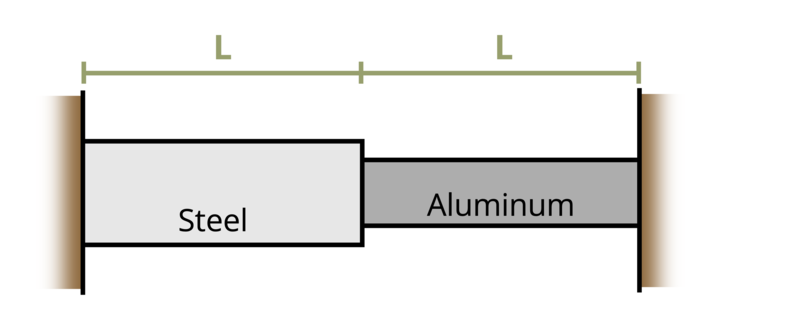
\includegraphics[keepaspectratio]{images/264.png}}
{[}Problem adapted from © Kurt Gramoll CC BY NC-SA 4.0{]}

\begin{Shaded}
\begin{Highlighting}[]
\NormalTok{\#| standalone: true}
\NormalTok{\#| viewerHeight: 600}
\NormalTok{\#| components: [viewer]}

\NormalTok{from shiny import App, render, ui, reactive}
\NormalTok{import random}
\NormalTok{import asyncio}
\NormalTok{import io}
\NormalTok{import math}
\NormalTok{import string}
\NormalTok{from datetime import datetime}
\NormalTok{from pathlib import Path}

\NormalTok{def generate\_random\_letters(length):}
\NormalTok{    \# Generate a random string of letters of specified length}
\NormalTok{    return \textquotesingle{}\textquotesingle{}.join(random.choice(string.ascii\_lowercase) for \_ in range(length))}

\NormalTok{problem\_ID="264"}
\NormalTok{L=reactive.Value("\_\_")}
\NormalTok{delT=reactive.Value("\_\_")}
\NormalTok{Aa=reactive.Value("\_\_")}
\NormalTok{As=reactive.Value("\_\_")}

\NormalTok{attempts=["Timestamp,Attempt,Answer,Feedback\textbackslash{}n"]}

\NormalTok{app\_ui = ui.page\_fluid(}
\NormalTok{    \#ui.markdown("**Please enter your ID number from your instructor and click to generate your problem**"),}
\NormalTok{    \#ui.input\_text("ID","", placeholder="Enter ID Number Here"),}
\NormalTok{    \#ui.input\_action\_button("generate\_problem", "Generate Problem", class\_="btn{-}primary"),}
\NormalTok{    ui.markdown("**Problem Statement**"),}
\NormalTok{    ui.output\_ui("ui\_problem\_statement"),}
\NormalTok{    ui.input\_text("answer","Your Answer in units of MPa", placeholder="Please enter your answer"),}
\NormalTok{    ui.input\_action\_button("submit", "Check Answer", class\_="btn{-}primary"),}
\NormalTok{    \#ui.download\_button("download", "Download File to Submit", class\_="btn{-}success"),}
\NormalTok{)}

\NormalTok{def server(input, output, session):}
\NormalTok{    \# Initialize a counter for attempts}
\NormalTok{    attempt\_counter = reactive.Value(0)}

\NormalTok{    @output}
\NormalTok{    @render.ui}
\NormalTok{    def ui\_problem\_statement():}
\NormalTok{        randomize\_vars()}
\NormalTok{        return[ui.markdown(f"Two members, each of length L = \{L()\} m., are placed between two fixed walls and heated by amount ΔT = \{delT()\}°C. The steel member (E\textless{}sub\textgreater{}s\textless{}/sub\textgreater{} = 200 GPa, α\textless{}sub\textgreater{}s\textless{}/sub\textgreater{} = 12 x 10\textless{}sup\textgreater{}{-}6\textless{}/sup\textgreater{} /°C) has cross{-}sectional area A\textless{}sub\textgreater{}s\textless{}/sub\textgreater{} = \{As()\} mm.\textless{}sup\textgreater{}2\textless{}/sup\textgreater{}. The aluminum member (E\textless{}sub\textgreater{}a\textless{}/sub\textgreater{} = 70 GPa, α\textless{}sub\textgreater{}a\textless{}/sub\textgreater{} = 23 x 10\textless{}sup\textgreater{}{-}6\textless{}/sup\textgreater{} /°C) has cross{-}sectional area A\textless{}sub\textgreater{}a\textless{}/sub\textgreater{} = \{Aa()\} mm.\textless{}sup\textgreater{}2\textless{}/sup\textgreater{}. Determine the average normal stress in the aluminum member.")]}
    
\NormalTok{    \#@reactive.Effect}
\NormalTok{    \#@reactive.event(input.generate\_problem)}
\NormalTok{    def randomize\_vars():}
\NormalTok{        random.seed(101)}
\NormalTok{        L.set(random.randrange(5,50,1)/10)}
\NormalTok{        delT.set(random.randrange(50,150,1))}
\NormalTok{        Aa.set(random.randrange(100,500,10))}
\NormalTok{        As.set(Aa()*2)}
    
\NormalTok{    @reactive.Effect}
\NormalTok{    @reactive.event(input.submit)}
\NormalTok{    def \_():}
\NormalTok{        attempt\_counter.set(attempt\_counter() + 1)  \# Increment the attempt counter on each submission.}
\NormalTok{        F = (12*10**{-}6*L()*delT()+23*10**{-}6*L()*delT())/(L()/(As()*200*10**3)+L()/(Aa()*70*10**3))}
\NormalTok{        instr = F/Aa()}
\NormalTok{        if math.isclose(float(input.answer()), instr, rel\_tol=0.01):}
\NormalTok{            check = "*Correct*"}
\NormalTok{            correct\_indicator = "JL"}
\NormalTok{        else:}
\NormalTok{            check = "*Not Correct.*"}
\NormalTok{            correct\_indicator = "JG"}

\NormalTok{        \# Generate random parts for the encoded attempt.}
\NormalTok{        random\_start = generate\_random\_letters(4)}
\NormalTok{        random\_middle = generate\_random\_letters(4)}
\NormalTok{        random\_end = generate\_random\_letters(4)}
\NormalTok{        \#encoded\_attempt = f"\{random\_start\}\{problem\_ID\}{-}\{random\_middle\}\{attempt\_counter()\}\{correct\_indicator\}{-}\{random\_end\}\{input.ID()\}"}

\NormalTok{        \# Store the most recent encoded attempt in a reactive value so it persists across submissions}
\NormalTok{        \#session.encoded\_attempt = reactive.Value(encoded\_attempt)}

\NormalTok{        \# Append the attempt data to the attempts list without the encoded attempt}
\NormalTok{        attempts.append(f"\{datetime.now()\}, \{attempt\_counter()\}, \{input.answer()\}, \{check\}\textbackslash{}n")}

\NormalTok{        \# Show feedback to the user.}
\NormalTok{        feedback = ui.markdown(f"Your answer of \{input.answer()\} is \{check\}.")}
\NormalTok{        m = ui.modal(}
\NormalTok{            feedback,}
\NormalTok{            title="Feedback",}
\NormalTok{            easy\_close=True}
\NormalTok{        )}
\NormalTok{        ui.modal\_show(m)}

\NormalTok{    \#@render.download(filename=lambda: f"Problem\_Log{-}\{problem\_ID\}{-}\{input.ID()\}.csv")}
\NormalTok{    async def download():}
\NormalTok{        \# Start the CSV with the encoded attempt (without label)}
\NormalTok{        final\_encoded = session.encoded\_attempt() if session.encoded\_attempt is not None else "No attempts"}
\NormalTok{        yield f"\{final\_encoded\}\textbackslash{}n\textbackslash{}n"}
        
\NormalTok{        \# Write the header for the remaining CSV data once}
\NormalTok{        yield "Timestamp,Attempt,Answer,Feedback\textbackslash{}n"}
        
\NormalTok{        \# Write the attempts data, ensure that the header from the attempts list is not written again}
\NormalTok{        for attempt in attempts[1:]:  \# Skip the first element which is the header}
\NormalTok{            await asyncio.sleep(0.25)  \# This delay may not be necessary; adjust as needed}
\NormalTok{            yield attempt}

\NormalTok{\# App installation}
\NormalTok{app = App(app\_ui, server)}
\end{Highlighting}
\end{Shaded}

\chapter*{Problem 5.50 - Thermal
Deformation}\label{problem-5.50---thermal-deformation}
\addcontentsline{toc}{chapter}{Problem 5.50 - Thermal Deformation}

\markboth{Problem 5.50 - Thermal Deformation}{Problem 5.50 - Thermal
Deformation}

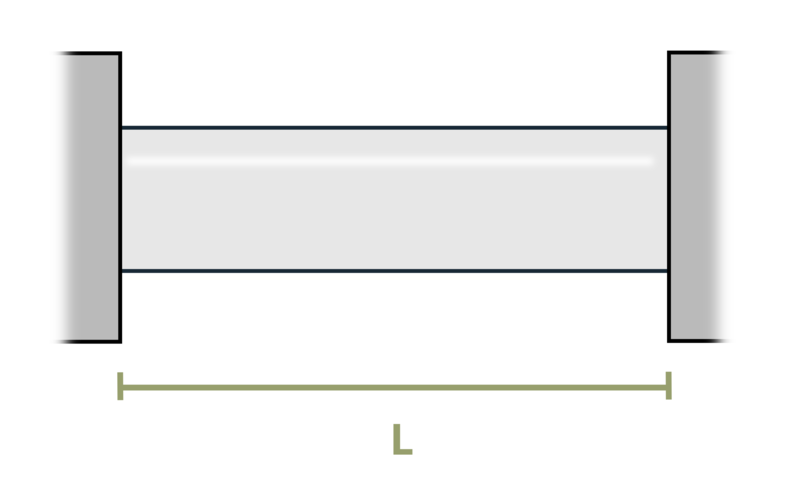
\includegraphics[width=3.125in,height=\textheight,keepaspectratio]{images/222.png}
{[}Problem adapted from © Kurt Gramoll CC BY NC-SA 4.0{]}

\begin{Shaded}
\begin{Highlighting}[]
\NormalTok{\#| standalone: true}
\NormalTok{\#| viewerHeight: 600}
\NormalTok{\#| components: [viewer]}

\NormalTok{from shiny import App, render, ui, reactive}
\NormalTok{import random}
\NormalTok{import asyncio}
\NormalTok{import io}
\NormalTok{import math}
\NormalTok{import string}
\NormalTok{from datetime import datetime}
\NormalTok{from pathlib import Path}

\NormalTok{def generate\_random\_letters(length):}
\NormalTok{    \# Generate a random string of letters of specified length}
\NormalTok{    return \textquotesingle{}\textquotesingle{}.join(random.choice(string.ascii\_lowercase) for \_ in range(length)) }

\NormalTok{problem\_ID="222"}
\NormalTok{stress=reactive.Value("\_\_")}
\NormalTok{L=reactive.Value("\_\_")}
\NormalTok{E=29000}
\NormalTok{alpha=6.5*10**{-}6}

\NormalTok{attempts=["Timestamp,Attempt,Answer,Feedback\textbackslash{}n"]}

\NormalTok{app\_ui = ui.page\_fluid(}
\NormalTok{    \#ui.markdown("**Please enter your ID number from your instructor and click to generate your problem**"),}
\NormalTok{    \#ui.input\_text("ID","", placeholder="Enter ID Number Here"),}
\NormalTok{    \#ui.input\_action\_button("generate\_problem", "Generate Problem", class\_="btn{-}primary"),}
\NormalTok{    ui.markdown("**Problem Statement**"),}
\NormalTok{    ui.output\_ui("ui\_problem\_statement"),}
\NormalTok{    ui.input\_text("answer","Your Answer in units of °F", placeholder="Please enter your answer"),}
\NormalTok{    ui.input\_action\_button("submit", "Check Answer", class\_="btn{-}primary"),}
\NormalTok{    \#ui.download\_button("download", "Download File to Submit", class\_="btn{-}success"),}
\NormalTok{)}


\NormalTok{def server(input, output, session):}
\NormalTok{    \# Initialize a counter for attempts}
\NormalTok{    attempt\_counter = reactive.Value(0)}

\NormalTok{    @output}
\NormalTok{    @render.ui}
\NormalTok{    def ui\_problem\_statement():}
\NormalTok{        randomize\_vars()}
\NormalTok{        return[ui.markdown(f"The axial stress in a solid circular bar between two fixed walls is \{stress()\} ksi. Find the temperature change necessary to relieve the stress. Assume L = \{L()\} in., E = 29,000 ksi, and α = 6.5 x 10\textless{}sup\textgreater{}{-}6\textless{}/sup\textgreater{} / °F. ")]}
    
\NormalTok{    \#@reactive.Effect}
\NormalTok{    \#@reactive.event(input.generate\_problem)}
\NormalTok{    def randomize\_vars():}
\NormalTok{        random.seed(101)}
\NormalTok{        stress.set(random.randrange(10, 150, 5))}
\NormalTok{        L.set(random.randrange(15, 75, 1))}
        
\NormalTok{    @reactive.Effect}
\NormalTok{    @reactive.event(input.submit)}
\NormalTok{    def \_():}
\NormalTok{        attempt\_counter.set(attempt\_counter() + 1)  \# Increment the attempt counter on each submission.}
\NormalTok{        instr= stress()/(alpha*E)}
\NormalTok{        if math.isclose(float(input.answer()), instr, rel\_tol=0.01):}
\NormalTok{            check = "*Correct*"}
\NormalTok{            correct\_indicator = "JL"}
\NormalTok{        else:}
\NormalTok{            check = "*Not Correct.*"}
\NormalTok{            correct\_indicator = "JG"}

\NormalTok{        \# Generate random parts for the encoded attempt.}
\NormalTok{        random\_start = generate\_random\_letters(4)}
\NormalTok{        random\_middle = generate\_random\_letters(4)}
\NormalTok{        random\_end = generate\_random\_letters(4)}
\NormalTok{        \#encoded\_attempt = f"\{random\_start\}\{problem\_ID\}{-}\{random\_middle\}\{attempt\_counter()\}\{correct\_indicator\}{-}\{random\_end\}\{input.ID()\}"}

\NormalTok{        \# Store the most recent encoded attempt in a reactive value so it persists across submissions}
\NormalTok{        \#session.encoded\_attempt = reactive.Value(encoded\_attempt)}

\NormalTok{        \# Append the attempt data to the attempts list without the encoded attempt}
\NormalTok{        attempts.append(f"\{datetime.now()\}, \{attempt\_counter()\}, \{input.answer()\}, \{check\}\textbackslash{}n")}

\NormalTok{        \# Show feedback to the user.}
\NormalTok{        feedback = ui.markdown(f"Your answer of \{input.answer()\} is \{check\}.")}
\NormalTok{        m = ui.modal(}
\NormalTok{            feedback,}
\NormalTok{            title="Feedback",}
\NormalTok{            easy\_close=True}
\NormalTok{        )}
\NormalTok{        ui.modal\_show(m)}

\NormalTok{    \#@render.download(filename=lambda: f"Problem\_Log{-}\{problem\_ID\}{-}\{input.ID()\}.csv")}
\NormalTok{    async def download():}
\NormalTok{        \# Start the CSV with the encoded attempt (without label)}
\NormalTok{        final\_encoded = session.encoded\_attempt() if session.encoded\_attempt is not None else "No attempts"}
\NormalTok{        yield f"\{final\_encoded\}\textbackslash{}n\textbackslash{}n"}
        
\NormalTok{        \# Write the header for the remaining CSV data once}
\NormalTok{        yield "Timestamp,Attempt,Answer,Feedback\textbackslash{}n"}
        
\NormalTok{        \# Write the attempts data, ensure that the header from the attempts list is not written again}
\NormalTok{        for attempt in attempts[1:]:  \# Skip the first element which is the header}
\NormalTok{            await asyncio.sleep(0.25)  \# This delay may not be necessary; adjust as needed}
\NormalTok{            yield attempt}


\NormalTok{\# App installation}
\NormalTok{app = App(app\_ui, server)}
\end{Highlighting}
\end{Shaded}

\chapter*{Problem 5.51 - Thermal
Deformation}\label{problem-5.51---thermal-deformation}
\addcontentsline{toc}{chapter}{Problem 5.51 - Thermal Deformation}

\markboth{Problem 5.51 - Thermal Deformation}{Problem 5.51 - Thermal
Deformation}

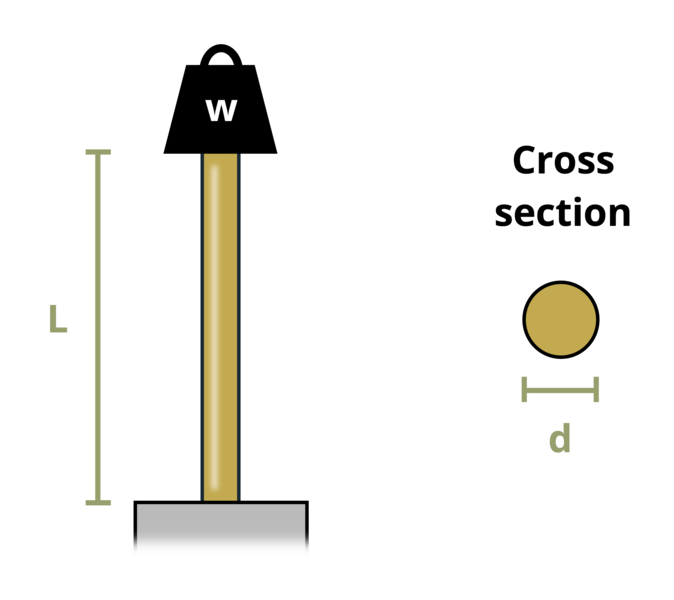
\includegraphics[width=3.125in,height=\textheight,keepaspectratio]{images/223.png}
{[}Problem adapted from © Kurt Gramoll CC BY NC-SA 4.0{]}

\begin{Shaded}
\begin{Highlighting}[]
\NormalTok{\#| standalone: true}
\NormalTok{\#| viewerHeight: 600}
\NormalTok{\#| components: [viewer]}

\NormalTok{from shiny import App, render, ui, reactive}
\NormalTok{import random}
\NormalTok{import asyncio}
\NormalTok{import io}
\NormalTok{import math}
\NormalTok{import string}
\NormalTok{from datetime import datetime}
\NormalTok{from pathlib import Path}

\NormalTok{def generate\_random\_letters(length):}
\NormalTok{    \# Generate a random string of letters of specified length}
\NormalTok{    return \textquotesingle{}\textquotesingle{}.join(random.choice(string.ascii\_lowercase) for \_ in range(length)) }

\NormalTok{problem\_ID="223"}
\NormalTok{W=reactive.Value("\_\_")}
\NormalTok{d=reactive.Value("\_\_")}
\NormalTok{L=reactive.Value("\_\_")}
\NormalTok{TC=reactive.Value("\_\_")}
\NormalTok{E=100*10**9}
\NormalTok{alpha=10*10**{-}6}

\NormalTok{attempts=["Timestamp,Attempt,Answer,Feedback\textbackslash{}n"]}

\NormalTok{app\_ui = ui.page\_fluid(}
\NormalTok{    \#ui.markdown("**Please enter your ID number from your instructor and click to generate your problem**"),}
\NormalTok{    \#ui.input\_text("ID","", placeholder="Enter ID Number Here"),}
\NormalTok{    \#ui.input\_action\_button("generate\_problem", "Generate Problem", class\_="btn{-}primary"),}
\NormalTok{    ui.markdown("**Problem Statement**"),}
\NormalTok{    ui.output\_ui("ui\_problem\_statement"),}
\NormalTok{    ui.input\_text("answer","Your Answer in units of mm", placeholder="Please enter your answer"),}
\NormalTok{    ui.input\_action\_button("submit", "Check Answer", class\_="btn{-}primary"),}
\NormalTok{    \#ui.download\_button("download", "Download File to Submit", class\_="btn{-}success"),}
\NormalTok{)}


\NormalTok{def server(input, output, session):}
\NormalTok{    \# Initialize a counter for attempts}
\NormalTok{    attempt\_counter = reactive.Value(0)}

\NormalTok{    @output}
\NormalTok{    @render.ui}
\NormalTok{    def ui\_problem\_statement():}
\NormalTok{        randomize\_vars()}
\NormalTok{        return[ui.markdown(f"The W = \{W()\} kg weight is placed on a L = \{L()\} m tall brass bar with a cross section of d = \{d()\} cm. If the bar undergoes a temperature change of \{TC()\}°C, what is the total deformation of the bar? Assume the Young\textquotesingle{}s Modulus and thermal coefficient of expansion is 100 GPa and 10 x 10\textless{}sup\textgreater{}{-}6\textless{}/sup\textgreater{} /°C, respectively. Also, assume no buckling. ")]}
    
\NormalTok{    \#@reactive.Effect}
\NormalTok{    \#@reactive.event(input.generate\_problem)}
\NormalTok{    def randomize\_vars():}
\NormalTok{        random.seed(101)}
\NormalTok{        W.set(random.randrange(500, 2000, 100))}
\NormalTok{        L.set(random.randrange(10, 50, 1)/10)}
\NormalTok{        d.set(random.randrange(15, 40, 1)/10)}
\NormalTok{        TC.set(random.randrange(20, 150, 5))}
        
        
\NormalTok{    @reactive.Effect}
\NormalTok{    @reactive.event(input.submit)}
\NormalTok{    def \_():}
\NormalTok{        attempt\_counter.set(attempt\_counter() + 1)  \# Increment the attempt counter on each submission.}
\NormalTok{        deltaT = L()*alpha*TC()}
\NormalTok{        deltaM = (W()*9.81*L())/(E*math.pi*(d()/200)**2) \#200 converts from diameter in cm to r in meters}
\NormalTok{        instr= (deltaT {-} deltaM)*1000 \# *1000 to get answer in mm}
\NormalTok{        if math.isclose(float(input.answer()), instr, rel\_tol=0.01):}
\NormalTok{            check = "*Correct*"}
\NormalTok{            correct\_indicator = "JL"}
\NormalTok{        else:}
\NormalTok{            check = "*Not Correct.*"}
\NormalTok{            correct\_indicator = "JG"}

\NormalTok{        \# Generate random parts for the encoded attempt.}
\NormalTok{        random\_start = generate\_random\_letters(4)}
\NormalTok{        random\_middle = generate\_random\_letters(4)}
\NormalTok{        random\_end = generate\_random\_letters(4)}
\NormalTok{        \#encoded\_attempt = f"\{random\_start\}\{problem\_ID\}{-}\{random\_middle\}\{attempt\_counter()\}\{correct\_indicator\}{-}\{random\_end\}\{input.ID()\}"}

\NormalTok{        \# Store the most recent encoded attempt in a reactive value so it persists across submissions}
\NormalTok{        \#session.encoded\_attempt = reactive.Value(encoded\_attempt)}

\NormalTok{        \# Append the attempt data to the attempts list without the encoded attempt}
\NormalTok{        attempts.append(f"\{datetime.now()\}, \{attempt\_counter()\}, \{input.answer()\}, \{check\}\textbackslash{}n")}

\NormalTok{        \# Show feedback to the user.}
\NormalTok{        feedback = ui.markdown(f"Your answer of \{input.answer()\} is \{check\}.")}
\NormalTok{        m = ui.modal(}
\NormalTok{            feedback,}
\NormalTok{            title="Feedback",}
\NormalTok{            easy\_close=True}
\NormalTok{        )}
\NormalTok{        ui.modal\_show(m)}

\NormalTok{    \#@render.download(filename=lambda: f"Problem\_Log{-}\{problem\_ID\}{-}\{input.ID()\}.csv")}
\NormalTok{    async def download():}
\NormalTok{        \# Start the CSV with the encoded attempt (without label)}
\NormalTok{        final\_encoded = session.encoded\_attempt() if session.encoded\_attempt is not None else "No attempts"}
\NormalTok{        yield f"\{final\_encoded\}\textbackslash{}n\textbackslash{}n"}
        
\NormalTok{        \# Write the header for the remaining CSV data once}
\NormalTok{        yield "Timestamp,Attempt,Answer,Feedback\textbackslash{}n"}
        
\NormalTok{        \# Write the attempts data, ensure that the header from the attempts list is not written again}
\NormalTok{        for attempt in attempts[1:]:  \# Skip the first element which is the header}
\NormalTok{            await asyncio.sleep(0.25)  \# This delay may not be necessary; adjust as needed}
\NormalTok{            yield attempt}


\NormalTok{\# App installation}
\NormalTok{app = App(app\_ui, server)}
\end{Highlighting}
\end{Shaded}

\chapter*{Problem 5.52 - Thermal
Deformation}\label{problem-5.52---thermal-deformation}
\addcontentsline{toc}{chapter}{Problem 5.52 - Thermal Deformation}

\markboth{Problem 5.52 - Thermal Deformation}{Problem 5.52 - Thermal
Deformation}

\pandocbounded{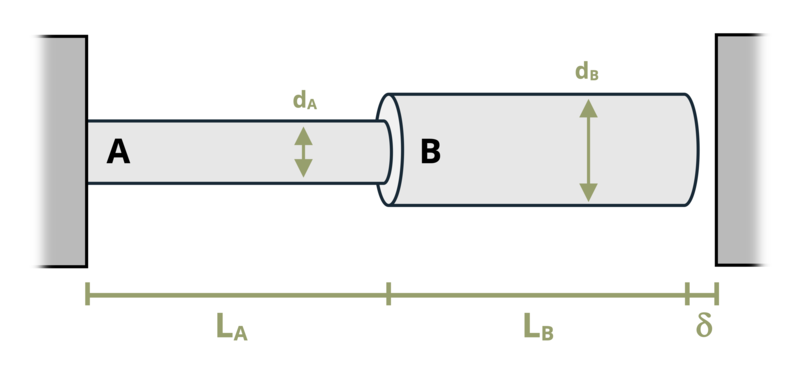
\includegraphics[keepaspectratio]{images/224.png}}
{[}Problem adapted from © Kurt Gramoll CC BY NC-SA 4.0{]}

\begin{Shaded}
\begin{Highlighting}[]
\NormalTok{\#| standalone: true}
\NormalTok{\#| viewerHeight: 600}
\NormalTok{\#| components: [viewer]}

\NormalTok{from shiny import App, render, ui, reactive}
\NormalTok{import random}
\NormalTok{import asyncio}
\NormalTok{import io}
\NormalTok{import math}
\NormalTok{import string}
\NormalTok{from datetime import datetime}
\NormalTok{from pathlib import Path}

\NormalTok{def generate\_random\_letters(length):}
\NormalTok{    \# Generate a random string of letters of specified length}
\NormalTok{    return \textquotesingle{}\textquotesingle{}.join(random.choice(string.ascii\_lowercase) for \_ in range(length)) }

\NormalTok{problem\_ID="224"}
\NormalTok{d=reactive.Value("\_\_")}
\NormalTok{rA=reactive.Value("\_\_")}
\NormalTok{rB=reactive.Value("\_\_")}
\NormalTok{L1=reactive.Value("\_\_")}
\NormalTok{L2=reactive.Value("\_\_")}
\NormalTok{alphaA=6*10**{-}6}
\NormalTok{alphaB=10*10**{-}6}

\NormalTok{attempts=["Timestamp,Attempt,Answer,Feedback\textbackslash{}n"]}

\NormalTok{app\_ui = ui.page\_fluid(}
\NormalTok{    \#ui.markdown("**Please enter your ID number from your instructor and click to generate your problem**"),}
\NormalTok{    \#ui.input\_text("ID","", placeholder="Enter ID Number Here"),}
\NormalTok{    \#ui.input\_action\_button("generate\_problem", "Generate Problem", class\_="btn{-}primary"),}
\NormalTok{    ui.markdown("**Problem Statement**"),}
\NormalTok{    ui.output\_ui("ui\_problem\_statement"),}
\NormalTok{    ui.input\_text("answer","Your Answer in units of °F", placeholder="Please enter your answer"),}
\NormalTok{    ui.input\_action\_button("submit", "Check Answer", class\_="btn{-}primary"),}
\NormalTok{    \#ui.download\_button("download", "Download File to Submit", class\_="btn{-}success"),}
\NormalTok{)}


\NormalTok{def server(input, output, session):}
\NormalTok{    \# Initialize a counter for attempts}
\NormalTok{    attempt\_counter = reactive.Value(0)}

\NormalTok{    @output}
\NormalTok{    @render.ui}
\NormalTok{    def ui\_problem\_statement():}
\NormalTok{        randomize\_vars()}
\NormalTok{        return[ui.markdown(f"Two cylindrical rods are heated until they expand, just closing the gap of d = \{d()\} in. The coefficient of thermal expansion, α, for material A and B is 6 x 10\textless{}sup\textgreater{}{-}6\textless{}/sup\textgreater{}/°F and 10 x 10\textless{}sup\textgreater{}{-}6\textless{}/sup\textgreater{}/°F, respectively. The radius of r\textless{}sub\textgreater{}A\textless{}/sub\textgreater{} = \{rA()\} in and the length is L\textless{}sub\textgreater{}A\textless{}/sub\textgreater{} = \{L1()\} in. The radius of B is r\textless{}sub\textgreater{}B\textless{}/sub\textgreater{} = \{rB()\} in and the length is L\textless{}sub\textgreater{}B\textless{}/sub\textgreater{} = \{L2()\} in. What is the change in temperature.  ")]}
    
\NormalTok{    \#@reactive.Effect}
\NormalTok{    \#@reactive.event(input.generate\_problem)}
\NormalTok{    def randomize\_vars():}
\NormalTok{        random.seed(101)}
\NormalTok{        d.set(random.randrange(1, 20, 1)/100)}
\NormalTok{        rA.set(random.randrange(5, 20, 1)/10)}
\NormalTok{        rB.set(round(rA()*1.6, 2))}
\NormalTok{        L1.set(random.randrange(5, 20, 1))}
\NormalTok{        L2.set(round(L1()*0.6, 2))}
        
        
\NormalTok{    @reactive.Effect}
\NormalTok{    @reactive.event(input.submit)}
\NormalTok{    def \_():}
\NormalTok{        attempt\_counter.set(attempt\_counter() + 1)  \# Increment the attempt counter on each submission.}
\NormalTok{        instr= d()/(alphaA*L1()+alphaB*L2())}
\NormalTok{        if math.isclose(float(input.answer()), instr, rel\_tol=0.01):}
\NormalTok{            check = "*Correct*"}
\NormalTok{            correct\_indicator = "JL"}
\NormalTok{        else:}
\NormalTok{            check = "*Not Correct.*"}
\NormalTok{            correct\_indicator = "JG"}

\NormalTok{        \# Generate random parts for the encoded attempt.}
\NormalTok{        random\_start = generate\_random\_letters(4)}
\NormalTok{        random\_middle = generate\_random\_letters(4)}
\NormalTok{        random\_end = generate\_random\_letters(4)}
\NormalTok{        \#encoded\_attempt = f"\{random\_start\}\{problem\_ID\}{-}\{random\_middle\}\{attempt\_counter()\}\{correct\_indicator\}{-}\{random\_end\}\{input.ID()\}"}

\NormalTok{        \# Store the most recent encoded attempt in a reactive value so it persists across submissions}
\NormalTok{        \#session.encoded\_attempt = reactive.Value(encoded\_attempt)}

\NormalTok{        \# Append the attempt data to the attempts list without the encoded attempt}
\NormalTok{        attempts.append(f"\{datetime.now()\}, \{attempt\_counter()\}, \{input.answer()\}, \{check\}\textbackslash{}n")}

\NormalTok{        \# Show feedback to the user.}
\NormalTok{        feedback = ui.markdown(f"Your answer of \{input.answer()\} is \{check\}.")}
\NormalTok{        m = ui.modal(}
\NormalTok{            feedback,}
\NormalTok{            title="Feedback",}
\NormalTok{            easy\_close=True}
\NormalTok{        )}
\NormalTok{        ui.modal\_show(m)}

\NormalTok{    \#@render.download(filename=lambda: f"Problem\_Log{-}\{problem\_ID\}{-}\{input.ID()\}.csv")}
\NormalTok{    async def download():}
\NormalTok{        \# Start the CSV with the encoded attempt (without label)}
\NormalTok{        final\_encoded = session.encoded\_attempt() if session.encoded\_attempt is not None else "No attempts"}
\NormalTok{        yield f"\{final\_encoded\}\textbackslash{}n\textbackslash{}n"}
        
\NormalTok{        \# Write the header for the remaining CSV data once}
\NormalTok{        yield "Timestamp,Attempt,Answer,Feedback\textbackslash{}n"}
        
\NormalTok{        \# Write the attempts data, ensure that the header from the attempts list is not written again}
\NormalTok{        for attempt in attempts[1:]:  \# Skip the first element which is the header}
\NormalTok{            await asyncio.sleep(0.25)  \# This delay may not be necessary; adjust as needed}
\NormalTok{            yield attempt}


\NormalTok{\# App installation}
\NormalTok{app = App(app\_ui, server)}
\end{Highlighting}
\end{Shaded}

\chapter*{Problem 5.53 - Thermal
Deformation}\label{problem-5.53---thermal-deformation}
\addcontentsline{toc}{chapter}{Problem 5.53 - Thermal Deformation}

\markboth{Problem 5.53 - Thermal Deformation}{Problem 5.53 - Thermal
Deformation}

\pandocbounded{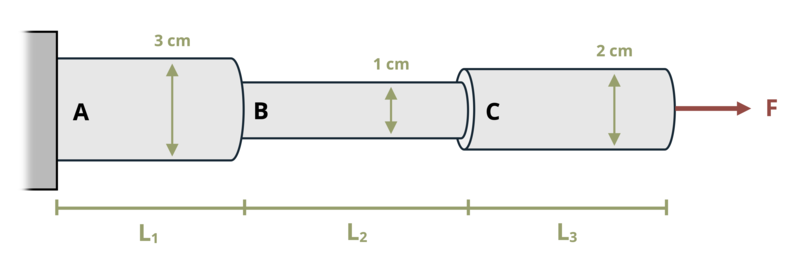
\includegraphics[keepaspectratio]{images/225.png}}
{[}Problem adapted from © Kurt Gramoll CC BY NC-SA 4.0{]}

\begin{Shaded}
\begin{Highlighting}[]
\NormalTok{\#| standalone: true}
\NormalTok{\#| viewerHeight: 600}
\NormalTok{\#| components: [viewer]}

\NormalTok{from shiny import App, render, ui, reactive}
\NormalTok{import random}
\NormalTok{import asyncio}
\NormalTok{import io}
\NormalTok{import math}
\NormalTok{import string}
\NormalTok{from datetime import datetime}
\NormalTok{from pathlib import Path}

\NormalTok{def generate\_random\_letters(length):}
\NormalTok{    \# Generate a random string of letters of specified length}
\NormalTok{    return \textquotesingle{}\textquotesingle{}.join(random.choice(string.ascii\_lowercase) for \_ in range(length)) }

\NormalTok{problem\_ID="225"}
\NormalTok{L1=reactive.Value("\_\_")}
\NormalTok{L2=reactive.Value("\_\_")}
\NormalTok{L3=reactive.Value("\_\_")}
\NormalTok{F=reactive.Value("\_\_")}
\NormalTok{dT=reactive.Value("\_\_")}
\NormalTok{alphaA=10*10**{-}6}
\NormalTok{alphaB=5*10**{-}6}
\NormalTok{alphaC=7*10**{-}6}
\NormalTok{EA=40*10**9}
\NormalTok{EB=120*10**9}
\NormalTok{EC=80*10**9}

\NormalTok{attempts=["Timestamp,Attempt,Answer,Feedback\textbackslash{}n"]}

\NormalTok{app\_ui = ui.page\_fluid(}
\NormalTok{    \#ui.markdown("**Please enter your ID number from your instructor and click to generate your problem**"),}
\NormalTok{    \#ui.input\_text("ID","", placeholder="Enter ID Number Here"),}
\NormalTok{    \#ui.input\_action\_button("generate\_problem", "Generate Problem", class\_="btn{-}primary"),}
\NormalTok{    ui.markdown("**Problem Statement**"),}
\NormalTok{    ui.output\_ui("ui\_problem\_statement"),}
\NormalTok{    ui.input\_text("answer","Your Answer in units of mm", placeholder="Please enter your answer"),}
\NormalTok{    ui.input\_action\_button("submit", "Check Answer", class\_="btn{-}primary"),}
\NormalTok{    \#ui.download\_button("download", "Download File to Submit", class\_="btn{-}success"),}
\NormalTok{)}


\NormalTok{def server(input, output, session):}
\NormalTok{    \# Initialize a counter for attempts}
\NormalTok{    attempt\_counter = reactive.Value(0)}

\NormalTok{    @output}
\NormalTok{    @render.ui}
\NormalTok{    def ui\_problem\_statement():}
\NormalTok{        randomize\_vars()}
\NormalTok{        return[ui.markdown(f"Three cylindrical rods of lengths L\textless{}sub\textgreater{}1\textless{}/sub\textgreater{} = \{L1()\} m, L\textless{}sub\textgreater{}2\textless{}/sub\textgreater{} = \{L2()\} m, and L\textless{}sub\textgreater{}3\textless{}/sub\textgreater{} = \{L3()\} m are connected together. A force F = \{F()\} kN is applied to the free end and all three rods are heated by \{dT()\} °C. The coefficient of thermal expansion, α, and elastic modulus, E, for each material are α\textless{}sub\textgreater{}A\textless{}/sub\textgreater{} = 10 x 10\textless{}sup\textgreater{}{-}6\textless{}/sup\textgreater{} /°C, α\textless{}sub\textgreater{}B\textless{}/sub\textgreater{} = 5 x 10\textless{}sup\textgreater{}{-}6\textless{}/sup\textgreater{} /°C, α\textless{}sub\textgreater{}C\textless{}/sub\textgreater{} = 7 x 10\textless{}sup\textgreater{}{-}6\textless{}/sup\textgreater{} /°C, E\textless{}sub\textgreater{}A\textless{}/sub\textgreater{} = 40 GPa, E\textless{}sub\textgreater{}B\textless{}/sub\textgreater{} = 120 GPa, and E\textless{}sub\textgreater{}C\textless{}/sub\textgreater{} = 80 GPa. What is the total deflection of the right rod tip?  ")]}
    
\NormalTok{    \#@reactive.Effect}
\NormalTok{    \#@reactive.event(input.generate\_problem)}
\NormalTok{    def randomize\_vars():}
\NormalTok{        random.seed(101)}
\NormalTok{        L1.set(random.randrange(10, 40, 1)/10)}
\NormalTok{        L2.set(round((L1()*0.8),1))}
\NormalTok{        L3.set(round((L1()*2/3),1))        }
\NormalTok{        F.set(random.randrange(5, 50, 1))}
\NormalTok{        dT.set(random.randrange(100, 300, 10))}
        
\NormalTok{    @reactive.Effect}
\NormalTok{    @reactive.event(input.submit)}
\NormalTok{    def \_():}
\NormalTok{        attempt\_counter.set(attempt\_counter() + 1)  \# Increment the attempt counter on each submission.}
\NormalTok{        deltaL = (F()*L1()*1000)/(EA*math.pi*.015**2) + (F()*L2()*1000)/(EB*math.pi*.005**2) + (F()*L3()*1000)/(EC*math.pi*.01**2)}
\NormalTok{        deltaT = alphaA*dT()*L1() + alphaB*dT()*L2() + alphaC*dT()*L3() }
\NormalTok{        instr= (deltaL + deltaT)*1000}
\NormalTok{        if math.isclose(float(input.answer()), instr, rel\_tol=0.01):}
\NormalTok{            check = "*Correct*"}
\NormalTok{            correct\_indicator = "JL"}
\NormalTok{        else:}
\NormalTok{            check = "*Not Correct.*"}
\NormalTok{            correct\_indicator = "JG"}

\NormalTok{        \# Generate random parts for the encoded attempt.}
\NormalTok{        random\_start = generate\_random\_letters(4)}
\NormalTok{        random\_middle = generate\_random\_letters(4)}
\NormalTok{        random\_end = generate\_random\_letters(4)}
\NormalTok{        \#encoded\_attempt = f"\{random\_start\}\{problem\_ID\}{-}\{random\_middle\}\{attempt\_counter()\}\{correct\_indicator\}{-}\{random\_end\}\{input.ID()\}"}

\NormalTok{        \# Store the most recent encoded attempt in a reactive value so it persists across submissions}
\NormalTok{        \#session.encoded\_attempt = reactive.Value(encoded\_attempt)}

\NormalTok{        \# Append the attempt data to the attempts list without the encoded attempt}
\NormalTok{        attempts.append(f"\{datetime.now()\}, \{attempt\_counter()\}, \{input.answer()\}, \{check\}\textbackslash{}n")}

\NormalTok{        \# Show feedback to the user.}
\NormalTok{        feedback = ui.markdown(f"Your answer of \{input.answer()\} is \{check\}.")}
\NormalTok{        m = ui.modal(}
\NormalTok{            feedback,}
\NormalTok{            title="Feedback",}
\NormalTok{            easy\_close=True}
\NormalTok{        )}
\NormalTok{        ui.modal\_show(m)}

\NormalTok{    \#@render.download(filename=lambda: f"Problem\_Log{-}\{problem\_ID\}{-}\{input.ID()\}.csv")}
\NormalTok{    async def download():}
\NormalTok{        \# Start the CSV with the encoded attempt (without label)}
\NormalTok{        final\_encoded = session.encoded\_attempt() if session.encoded\_attempt is not None else "No attempts"}
\NormalTok{        yield f"\{final\_encoded\}\textbackslash{}n\textbackslash{}n"}
        
\NormalTok{        \# Write the header for the remaining CSV data once}
\NormalTok{        yield "Timestamp,Attempt,Answer,Feedback\textbackslash{}n"}
        
\NormalTok{        \# Write the attempts data, ensure that the header from the attempts list is not written again}
\NormalTok{        for attempt in attempts[1:]:  \# Skip the first element which is the header}
\NormalTok{            await asyncio.sleep(0.25)  \# This delay may not be necessary; adjust as needed}
\NormalTok{            yield attempt}

\NormalTok{\# App installation}
\NormalTok{app = App(app\_ui, server)}
\end{Highlighting}
\end{Shaded}

\chapter*{Problem 5.54 - Thermal
Deformation}\label{problem-5.54---thermal-deformation}
\addcontentsline{toc}{chapter}{Problem 5.54 - Thermal Deformation}

\markboth{Problem 5.54 - Thermal Deformation}{Problem 5.54 - Thermal
Deformation}

\pandocbounded{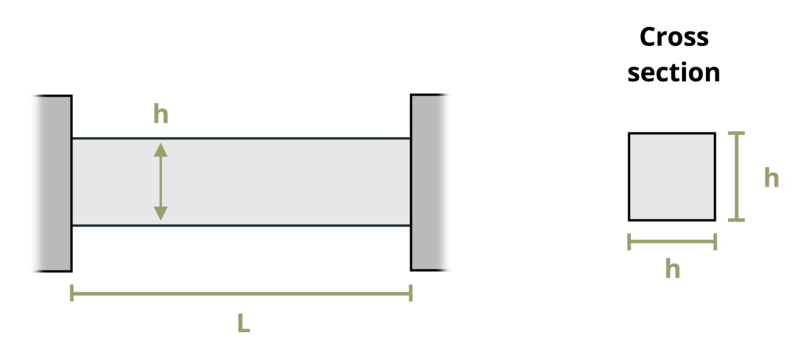
\includegraphics[keepaspectratio]{images/226.png}}
{[}Problem adapted from © Kurt Gramoll CC BY NC-SA 4.0{]}

\begin{Shaded}
\begin{Highlighting}[]
\NormalTok{\#| standalone: true}
\NormalTok{\#| viewerHeight: 600}
\NormalTok{\#| components: [viewer]}

\NormalTok{from shiny import App, render, ui, reactive}
\NormalTok{import random}
\NormalTok{import asyncio}
\NormalTok{import io}
\NormalTok{import math}
\NormalTok{import string}
\NormalTok{from datetime import datetime}
\NormalTok{from pathlib import Path}

\NormalTok{def generate\_random\_letters(length):}
\NormalTok{    \# Generate a random string of letters of specified length}
\NormalTok{    return \textquotesingle{}\textquotesingle{}.join(random.choice(string.ascii\_lowercase) for \_ in range(length)) }

\NormalTok{problem\_ID="226"}
\NormalTok{T1=reactive.Value("\_\_")}
\NormalTok{T2=reactive.Value("\_\_")}
\NormalTok{L=reactive.Value("\_\_")}
\NormalTok{h=reactive.Value("\_\_")}
\NormalTok{alpha=20*10**{-}6}
\NormalTok{E=100*10**9}

\NormalTok{attempts=["Timestamp,Attempt,Answer,Feedback\textbackslash{}n"]}

\NormalTok{app\_ui = ui.page\_fluid(}
\NormalTok{    \#ui.markdown("**Please enter your ID number from your instructor and click to generate your problem**"),}
\NormalTok{    \#ui.input\_text("ID","", placeholder="Enter ID Number Here"),}
\NormalTok{    \#ui.input\_action\_button("generate\_problem", "Generate Problem", class\_="btn{-}primary"),}
\NormalTok{    ui.markdown("**Problem Statement**"),}
\NormalTok{    ui.output\_ui("ui\_problem\_statement"),}
\NormalTok{    ui.input\_text("answer","Your Answer in units of MPa", placeholder="Please enter your answer"),}
\NormalTok{    ui.input\_action\_button("submit", "Check Answer", class\_="btn{-}primary"),}
\NormalTok{    \#ui.download\_button("download", "Download File to Submit", class\_="btn{-}success"),}
\NormalTok{)}


\NormalTok{def server(input, output, session):}
\NormalTok{    \# Initialize a counter for attempts}
\NormalTok{    attempt\_counter = reactive.Value(0)}

\NormalTok{    @output}
\NormalTok{    @render.ui}
\NormalTok{    def ui\_problem\_statement():}
\NormalTok{        randomize\_vars()}
\NormalTok{        return[ui.markdown(f"A square brass bar is placed between two fixed walls and heated from \{T1()\}°C to \{T2()\}°C. If L = \{L()\} mm, h = \{h()\} mm, E = 100 GPa, and α = 20 x 10\textless{}sup\textgreater{}{-}6\textless{}/sup\textgreater{} /°C, determine the stress in the bar.  ")]}
    
\NormalTok{    \#@reactive.Effect}
\NormalTok{    \#@reactive.event(input.generate\_problem)}
\NormalTok{    def randomize\_vars():}
\NormalTok{        random.seed(101)}
\NormalTok{        T1.set(random.randrange(5, 20, 1))}
\NormalTok{        T2.set(round(T1() + random.randrange(20, 50, 1), 2))}
\NormalTok{        L.set(random.randrange(250, 750, 10))}
\NormalTok{        h.set(random.randrange(10, 30, 1))}
       
        
\NormalTok{    @reactive.Effect}
\NormalTok{    @reactive.event(input.submit)}
\NormalTok{    def \_():}
\NormalTok{        attempt\_counter.set(attempt\_counter() + 1)  \# Increment the attempt counter on each submission.}
\NormalTok{        instr= (E*alpha*(T2(){-}T1()))/10**6}
\NormalTok{        if math.isclose(float(input.answer()), instr, rel\_tol=0.01):}
\NormalTok{            check = "*Correct*"}
\NormalTok{            correct\_indicator = "JL"}
\NormalTok{        else:}
\NormalTok{            check = "*Not Correct.*"}
\NormalTok{            correct\_indicator = "JG"}

\NormalTok{        \# Generate random parts for the encoded attempt.}
\NormalTok{        random\_start = generate\_random\_letters(4)}
\NormalTok{        random\_middle = generate\_random\_letters(4)}
\NormalTok{        random\_end = generate\_random\_letters(4)}
\NormalTok{        \#encoded\_attempt = f"\{random\_start\}\{problem\_ID\}{-}\{random\_middle\}\{attempt\_counter()\}\{correct\_indicator\}{-}\{random\_end\}\{input.ID()\}"}

\NormalTok{        \# Store the most recent encoded attempt in a reactive value so it persists across submissions}
\NormalTok{        \#session.encoded\_attempt = reactive.Value(encoded\_attempt)}

\NormalTok{        \# Append the attempt data to the attempts list without the encoded attempt}
\NormalTok{        attempts.append(f"\{datetime.now()\}, \{attempt\_counter()\}, \{input.answer()\}, \{check\}\textbackslash{}n")}

\NormalTok{        \# Show feedback to the user.}
\NormalTok{        feedback = ui.markdown(f"Your answer of \{input.answer()\} is \{check\}.")}
\NormalTok{        m = ui.modal(}
\NormalTok{            feedback,}
\NormalTok{            title="Feedback",}
\NormalTok{            easy\_close=True}
\NormalTok{        )}
\NormalTok{        ui.modal\_show(m)}

\NormalTok{    \#@render.download(filename=lambda: f"Problem\_Log{-}\{problem\_ID\}{-}\{input.ID()\}.csv")}
\NormalTok{    async def download():}
\NormalTok{        \# Start the CSV with the encoded attempt (without label)}
\NormalTok{        final\_encoded = session.encoded\_attempt() if session.encoded\_attempt is not None else "No attempts"}
\NormalTok{        yield f"\{final\_encoded\}\textbackslash{}n\textbackslash{}n"}
        
\NormalTok{        \# Write the header for the remaining CSV data once}
\NormalTok{        yield "Timestamp,Attempt,Answer,Feedback\textbackslash{}n"}
        
\NormalTok{        \# Write the attempts data, ensure that the header from the attempts list is not written again}
\NormalTok{        for attempt in attempts[1:]:  \# Skip the first element which is the header}
\NormalTok{            await asyncio.sleep(0.25)  \# This delay may not be necessary; adjust as needed}
\NormalTok{            yield attempt}


\NormalTok{\# App installation}
\NormalTok{app = App(app\_ui, server)}
\end{Highlighting}
\end{Shaded}

\chapter*{Problem 5.55 - Thermal
Deformation}\label{problem-5.55---thermal-deformation}
\addcontentsline{toc}{chapter}{Problem 5.55 - Thermal Deformation}

\markboth{Problem 5.55 - Thermal Deformation}{Problem 5.55 - Thermal
Deformation}

\pandocbounded{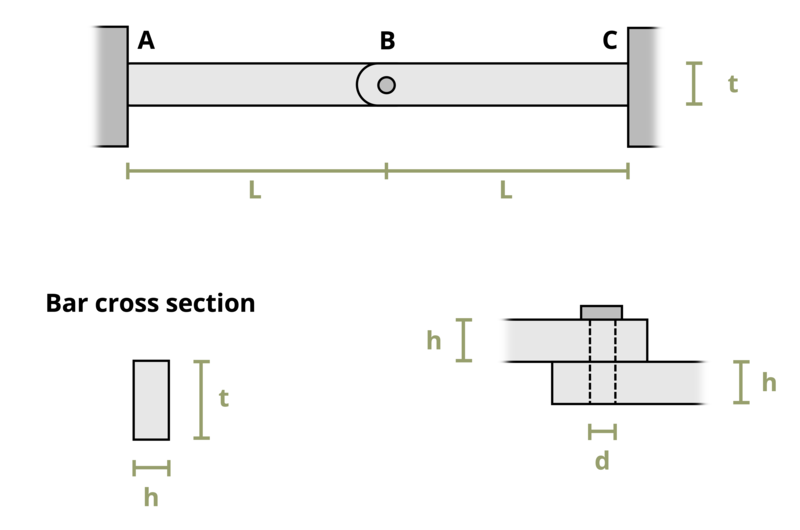
\includegraphics[keepaspectratio]{images/249.png}}
{[}Problem adapted from © Kurt Gramoll CC BY NC-SA 4.0{]}

\begin{Shaded}
\begin{Highlighting}[]
\NormalTok{\#| standalone: true}
\NormalTok{\#| viewerHeight: 600}
\NormalTok{\#| components: [viewer]}

\NormalTok{from shiny import App, render, ui, reactive}
\NormalTok{import random}
\NormalTok{import asyncio}
\NormalTok{import io}
\NormalTok{import math}
\NormalTok{import string}
\NormalTok{from datetime import datetime}
\NormalTok{from pathlib import Path}

\NormalTok{def generate\_random\_letters(length):}
\NormalTok{    \# Generate a random string of letters of specified length}
\NormalTok{    return \textquotesingle{}\textquotesingle{}.join(random.choice(string.ascii\_lowercase) for \_ in range(length)) }

\NormalTok{problem\_ID="249"}
\NormalTok{L=reactive.Value("\_\_")}
\NormalTok{d=reactive.Value("\_\_")}
\NormalTok{t=reactive.Value("\_\_")}
\NormalTok{h=reactive.Value("\_\_")}
\NormalTok{dT=reactive.Value("\_\_")}
\NormalTok{E=200}
\NormalTok{v=0.32}
\NormalTok{a=11.7*10**{-}6}

\NormalTok{attempts=["Timestamp,Attempt,Answer,Feedback\textbackslash{}n"]}

\NormalTok{app\_ui = ui.page\_fluid(}
\NormalTok{    \#ui.markdown("**Please enter your ID number from your instructor and click to generate your problem**"),}
\NormalTok{    \#ui.input\_text("ID","", placeholder="Enter ID Number Here"),}
\NormalTok{    \#ui.input\_action\_button("generate\_problem", "Generate Problem", class\_="btn{-}primary"),}
\NormalTok{    ui.markdown("**Problem Statement**"),}
\NormalTok{    ui.output\_ui("ui\_problem\_statement"),}
\NormalTok{    ui.input\_text("answer","Your Answer in units of MPa", placeholder="Please enter your answer"),}
\NormalTok{    ui.input\_action\_button("submit", "Check Answer", class\_="btn{-}primary"),}
\NormalTok{    \#ui.download\_button("download", "Download File to Submit", class\_="btn{-}success"),}
\NormalTok{)}


\NormalTok{def server(input, output, session):}
\NormalTok{    \# Initialize a counter for attempts}
\NormalTok{    attempt\_counter = reactive.Value(0)}

\NormalTok{    @output}
\NormalTok{    @render.ui}
\NormalTok{    def ui\_problem\_statement():}
\NormalTok{        randomize\_vars()}
\NormalTok{        return[ui.markdown(f"Bars AB and BC are pinned at joint B. Both bars are made from the same material with E = 200 GPa, v = 0.32, and a = 11.7 x 10\textless{}sup\textgreater{}{-}6\textless{}/sup\textgreater{} /°C. Dimensions L = \{L()\}  mm, t = \{t()\} mm, h = \{h()\} mm, and d = \{d()\} mm. If both bars are heated by \{dT()\} °C, determine the shear stress generated in the pin at B.")]}
    
\NormalTok{    \#@reactive.Effect}
\NormalTok{    \#@reactive.event(input.generate\_problem)}
\NormalTok{    def randomize\_vars():}
\NormalTok{        random.seed(101)}
\NormalTok{        L.set(random.randrange(300, 900, 10))}
\NormalTok{        t.set(random.randrange(30, 80, 1))}
\NormalTok{        h.set(t()/2)}
\NormalTok{        d.set(round(t()/3,2))}
\NormalTok{        dT.set(random.randrange(10, 40, 1))}
        
\NormalTok{    @reactive.Effect}
\NormalTok{    @reactive.event(input.submit)}
\NormalTok{    def \_():}
\NormalTok{        attempt\_counter.set(attempt\_counter() + 1)  \# Increment the attempt counter on each submission.}
\NormalTok{        deltaM = a*dT()*(t()/1000)*(h()/1000)*E*10**9}
\NormalTok{        instr= (deltaM/(math.pi*(d()/2000)**2))/10**6}
\NormalTok{        if math.isclose(float(input.answer()), instr, rel\_tol=0.01):}
\NormalTok{            check = "*Correct*"}
\NormalTok{            correct\_indicator = "JL"}
\NormalTok{        else:}
\NormalTok{            check = "*Not Correct.*"}
\NormalTok{            correct\_indicator = "JG"}

\NormalTok{        \# Generate random parts for the encoded attempt.}
\NormalTok{        random\_start = generate\_random\_letters(4)}
\NormalTok{        random\_middle = generate\_random\_letters(4)}
\NormalTok{        random\_end = generate\_random\_letters(4)}
\NormalTok{        \#encoded\_attempt = f"\{random\_start\}\{problem\_ID\}{-}\{random\_middle\}\{attempt\_counter()\}\{correct\_indicator\}{-}\{random\_end\}\{input.ID()\}"}

\NormalTok{        \# Store the most recent encoded attempt in a reactive value so it persists across submissions}
\NormalTok{        \#session.encoded\_attempt = reactive.Value(encoded\_attempt)}

\NormalTok{        \# Append the attempt data to the attempts list without the encoded attempt}
\NormalTok{        attempts.append(f"\{datetime.now()\}, \{attempt\_counter()\}, \{input.answer()\}, \{check\}\textbackslash{}n")}

\NormalTok{        \# Show feedback to the user.}
\NormalTok{        feedback = ui.markdown(f"Your answer of \{input.answer()\} is \{check\}.")}
\NormalTok{        m = ui.modal(}
\NormalTok{            feedback,}
\NormalTok{            title="Feedback",}
\NormalTok{            easy\_close=True}
\NormalTok{        )}
\NormalTok{        ui.modal\_show(m)}

\NormalTok{    \#@render.download(filename=lambda: f"Problem\_Log{-}\{problem\_ID\}{-}\{input.ID()\}.csv")}
\NormalTok{    async def download():}
\NormalTok{        \# Start the CSV with the encoded attempt (without label)}
\NormalTok{        final\_encoded = session.encoded\_attempt() if session.encoded\_attempt is not None else "No attempts"}
\NormalTok{        yield f"\{final\_encoded\}\textbackslash{}n\textbackslash{}n"}
        
\NormalTok{        \# Write the header for the remaining CSV data once}
\NormalTok{        yield "Timestamp,Attempt,Answer,Feedback\textbackslash{}n"}
        
\NormalTok{        \# Write the attempts data, ensure that the header from the attempts list is not written again}
\NormalTok{        for attempt in attempts[1:]:  \# Skip the first element which is the header}
\NormalTok{            await asyncio.sleep(0.25)  \# This delay may not be necessary; adjust as needed}
\NormalTok{            yield attempt}


\NormalTok{\# App installation}
\NormalTok{app = App(app\_ui, server)}
\end{Highlighting}
\end{Shaded}

\chapter*{Problem 5.56 - Thermal
Deformation}\label{problem-5.56---thermal-deformation}
\addcontentsline{toc}{chapter}{Problem 5.56 - Thermal Deformation}

\markboth{Problem 5.56 - Thermal Deformation}{Problem 5.56 - Thermal
Deformation}

\pandocbounded{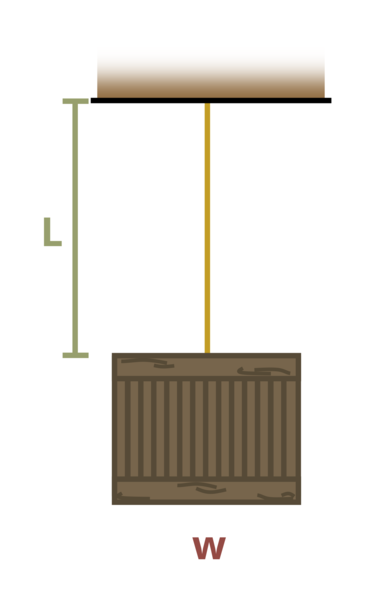
\includegraphics[keepaspectratio]{images/227.png}}
{[}Problem adapted from © Kurt Gramoll CC BY NC-SA 4.0{]}

\begin{Shaded}
\begin{Highlighting}[]
\NormalTok{\#| standalone: true}
\NormalTok{\#| viewerHeight: 600}
\NormalTok{\#| components: [viewer]}

\NormalTok{from shiny import App, render, ui, reactive}
\NormalTok{import random}
\NormalTok{import asyncio}
\NormalTok{import io}
\NormalTok{import math}
\NormalTok{import string}
\NormalTok{from datetime import datetime}
\NormalTok{from pathlib import Path}

\NormalTok{def generate\_random\_letters(length):}
\NormalTok{    \# Generate a random string of letters of specified length}
\NormalTok{    return \textquotesingle{}\textquotesingle{}.join(random.choice(string.ascii\_lowercase) for \_ in range(length))  }

\NormalTok{problem\_ID="227"}
\NormalTok{W=reactive.Value("\_\_")}
\NormalTok{L=reactive.Value("\_\_")}
\NormalTok{A=reactive.Value("\_\_")}
\NormalTok{T1=reactive.Value("\_\_")}
\NormalTok{T2 =reactive.Value("\_\_")}
  
\NormalTok{attempts=["Timestamp,Attempt,Answer,Feedback\textbackslash{}n"]}

\NormalTok{app\_ui = ui.page\_fluid(}
\NormalTok{    \#ui.markdown("**Please enter your ID number from your instructor and click to generate your problem**"),}
\NormalTok{    \#ui.input\_text("ID","", placeholder="Enter ID Number Here"),}
\NormalTok{    \#ui.input\_action\_button("generate\_problem", "Generate Problem", class\_="btn{-}primary"),}
\NormalTok{    ui.markdown("**Problem Statement**"),}
\NormalTok{    ui.output\_ui("ui\_problem\_statement"),}
\NormalTok{    ui.input\_text("answer","Your Answer in units of inches", placeholder="Please enter your answer"),}
\NormalTok{    ui.input\_action\_button("submit", "Check Answer", class\_="btn{-}primary"),}
\NormalTok{    \#ui.download\_button("download", "Download File to Submit", class\_="btn{-}success"),}
\NormalTok{)}


\NormalTok{def server(input, output, session):}
\NormalTok{    \# Initialize a counter for attempts}
\NormalTok{    attempt\_counter = reactive.Value(0)}

\NormalTok{    @output}
\NormalTok{    @render.ui}
\NormalTok{    def ui\_problem\_statement():}
\NormalTok{        randomize\_vars()}
\NormalTok{        return[ui.markdown(f"A crate weighting W = \{W()\} kips is attached to a brass cable of length L = \{L()\} in. and cross{-}sectional area A = \{A()\} in.\textless{}sup\textgreater{}2\textless{}/sup\textgreater{}. The temperature is increased from T\textless{}sub\textgreater{}1\textless{}/sub\textgreater{} = \{T1()\}°F to T\textless{}sub\textgreater{}2\textless{}/sub\textgreater{} = \{T2()\}°F. Determine the total change in lengh of the cable. Assume α = 11 x 10\textless{}sup\textgreater{}{-}6\textless{}/sup\textgreater{} /°F and E = 15,000 ksi.")]}
    
\NormalTok{    \#@reactive.Effect}
\NormalTok{    \#@reactive.event(input.generate\_problem)}
\NormalTok{    def randomize\_vars():}
\NormalTok{        random.seed(101)}
\NormalTok{        W.set(random.randrange(50, 200, 1))}
\NormalTok{        L.set(random.randrange(15, 30, 1))}
\NormalTok{        A.set(random.randrange(10, 50, 1))}
\NormalTok{        T1.set(random.randrange(20,50,1))}
\NormalTok{        T2.set(random.randrange(150,250,1))}
        

\NormalTok{    @reactive.Effect}
\NormalTok{    @reactive.event(input.submit)}
\NormalTok{    def \_():}
\NormalTok{        attempt\_counter.set(attempt\_counter() + 1)  \# Increment the attempt counter on each submission.}
    
\NormalTok{        instr= W()*L()/(A()*15000*1000)+11*10**({-}6)*(T2(){-}T1())*L()}
\NormalTok{        if math.isclose(float(input.answer()), instr, rel\_tol=0.01):}
\NormalTok{            check = "*Correct*"}
\NormalTok{            correct\_indicator = "JL"}
\NormalTok{        else:}
\NormalTok{            check = "*Not Correct.*"}
\NormalTok{            correct\_indicator = "JG"}

\NormalTok{        \# Generate random parts for the encoded attempt.}
\NormalTok{        random\_start = generate\_random\_letters(4)}
\NormalTok{        random\_middle = generate\_random\_letters(4)}
\NormalTok{        random\_end = generate\_random\_letters(4)}
\NormalTok{        \#encoded\_attempt = f"\{random\_start\}\{problem\_ID\}{-}\{random\_middle\}\{attempt\_counter()\}\{correct\_indicator\}{-}\{random\_end\}\{input.ID()\}"}

\NormalTok{        \# Store the most recent encoded attempt in a reactive value so it persists across submissions}
\NormalTok{        \#session.encoded\_attempt = reactive.Value(encoded\_attempt)}

\NormalTok{        \# Append the attempt data to the attempts list without the encoded attempt}
\NormalTok{        attempts.append(f"\{datetime.now()\}, \{attempt\_counter()\}, \{input.answer()\}, \{check\}\textbackslash{}n")}

\NormalTok{        \# Show feedback to the user.}
\NormalTok{        feedback = ui.markdown(f"Your answer of \{input.answer()\} is \{check\}.")}
\NormalTok{        m = ui.modal(}
\NormalTok{            feedback,}
\NormalTok{            title="Feedback",}
\NormalTok{            easy\_close=True}
\NormalTok{        )}
\NormalTok{        ui.modal\_show(m)}

\NormalTok{    \#@render.download(filename=lambda: f"Problem\_Log{-}\{problem\_ID\}{-}\{input.ID()\}.csv")}
\NormalTok{    async def download():}
\NormalTok{        \# Start the CSV with the encoded attempt (without label)}
\NormalTok{        final\_encoded = session.encoded\_attempt() if session.encoded\_attempt is not None else "No attempts"}
\NormalTok{        yield f"\{final\_encoded\}\textbackslash{}n\textbackslash{}n"}
        
\NormalTok{        \# Write the header for the remaining CSV data once}
\NormalTok{        yield "Timestamp,Attempt,Answer,Feedback\textbackslash{}n"}
        
\NormalTok{        \# Write the attempts data, ensure that the header from the attempts list is not written again}
\NormalTok{        for attempt in attempts[1:]:  \# Skip the first element which is the header}
\NormalTok{            await asyncio.sleep(0.25)  \# This delay may not be necessary; adjust as needed}
\NormalTok{            yield attempt}


\NormalTok{\# App installation}
\NormalTok{app = App(app\_ui, server)}
\end{Highlighting}
\end{Shaded}

\chapter*{Problem 5.57 - Thermal
Deformation}\label{problem-5.57---thermal-deformation}
\addcontentsline{toc}{chapter}{Problem 5.57 - Thermal Deformation}

\markboth{Problem 5.57 - Thermal Deformation}{Problem 5.57 - Thermal
Deformation}

\pandocbounded{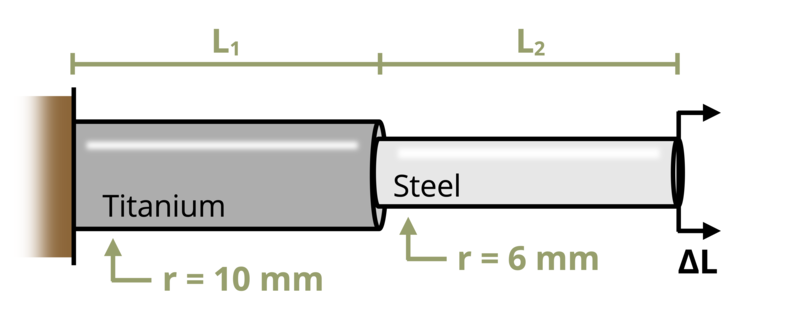
\includegraphics[keepaspectratio]{images/228.png}}
{[}Problem adapted from © Kurt Gramoll CC BY NC-SA 4.0{]}

\begin{Shaded}
\begin{Highlighting}[]
\NormalTok{\#| standalone: true}
\NormalTok{\#| viewerHeight: 600}
\NormalTok{\#| components: [viewer]}

\NormalTok{from shiny import App, render, ui, reactive}
\NormalTok{import random}
\NormalTok{import asyncio}
\NormalTok{import io}
\NormalTok{import math}
\NormalTok{import string}
\NormalTok{from datetime import datetime}
\NormalTok{from pathlib import Path}

\NormalTok{def generate\_random\_letters(length):}
\NormalTok{    \# Generate a random string of letters of specified length}
\NormalTok{    return \textquotesingle{}\textquotesingle{}.join(random.choice(string.ascii\_lowercase) for \_ in range(length))}

\NormalTok{problem\_ID="228"}
\NormalTok{L2=reactive.Value("\_\_")}
\NormalTok{L1=reactive.Value("\_\_")}
\NormalTok{delL=reactive.Value("\_\_")}
  
\NormalTok{attempts=["Timestamp,Attempt,Answer,Feedback\textbackslash{}n"]}

\NormalTok{app\_ui = ui.page\_fluid(}
\NormalTok{    \#ui.markdown("**Please enter your ID number from your instructor and click to generate your problem**"),}
\NormalTok{    \#ui.input\_text("ID","", placeholder="Enter ID Number Here"),}
\NormalTok{    \#ui.input\_action\_button("generate\_problem", "Generate Problem", class\_="btn{-}primary"),}
\NormalTok{    ui.markdown("**Problem Statement**"),}
\NormalTok{    ui.output\_ui("ui\_problem\_statement"),}
\NormalTok{    ui.input\_text("answer","Your Answer in units of \textbackslash{}u00b0C", placeholder="Please enter your answer"),}
\NormalTok{    ui.input\_action\_button("submit", "Check Answer", class\_="btn{-}primary"),}
\NormalTok{    \#ui.download\_button("download", "Download File to Submit", class\_="btn{-}success"),}
\NormalTok{)}

\NormalTok{def server(input, output, session):}
\NormalTok{    \# Initialize a counter for attempts}
\NormalTok{    attempt\_counter = reactive.Value(0)}

\NormalTok{    @output}
\NormalTok{    @render.ui}
\NormalTok{    def ui\_problem\_statement():}
\NormalTok{        randomize\_vars()}
\NormalTok{        return[ui.markdown(f"Two solid circular rods of lengths L\textless{}sub\textgreater{}1\textless{}/sub\textgreater{} = \{L1()\} mm and L\textless{}sub\textgreater{}2\textless{}/sub\textgreater{} = \{L2()\} mm are heated and the total change in length is measured as ΔL = \{delL()\} mm. Determine the change in temperature, assuming α\textless{}sub\textgreater{}t\textless{}/sub\textgreater{} = 9.5 x 10\textless{}sup\textgreater{}{-}6\textless{}/sup\textgreater{} /°C and α\textless{}sub\textgreater{}s\textless{}/sub\textgreater{} = 12 x 10\textless{}sup\textgreater{}{-}6\textless{}/sup\textgreater{} /°C.")]}
    
\NormalTok{    \#@reactive.Effect}
\NormalTok{    \#@reactive.event(input.generate\_problem)}
\NormalTok{    def randomize\_vars():}
\NormalTok{        random.seed(101)}
\NormalTok{        L2.set(random.randrange(400,600,10))}
\NormalTok{        L1.set(L2()+random.randrange(100,200,10))}
\NormalTok{        delL.set(random.randrange(10,300,1)/100)}
        
\NormalTok{    @reactive.Effect}
\NormalTok{    @reactive.event(input.submit)}
\NormalTok{    def \_():}
\NormalTok{        attempt\_counter.set(attempt\_counter() + 1)  \# Increment the attempt counter on each submission.}
\NormalTok{        instr = delL()/(L1()*9.5*10**({-}6)+L2()*12*10**({-}6))}
\NormalTok{        if math.isclose(float(input.answer()), instr, rel\_tol=0.01):}
\NormalTok{            check = "*Correct*"}
\NormalTok{            correct\_indicator = "JL"}
\NormalTok{        else:}
\NormalTok{            check = "*Not Correct.*"}
\NormalTok{            correct\_indicator = "JG"}

\NormalTok{        \# Generate random parts for the encoded attempt.}
\NormalTok{        random\_start = generate\_random\_letters(4)}
\NormalTok{        random\_middle = generate\_random\_letters(4)}
\NormalTok{        random\_end = generate\_random\_letters(4)}
\NormalTok{        \#encoded\_attempt = f"\{random\_start\}\{problem\_ID\}{-}\{random\_middle\}\{attempt\_counter()\}\{correct\_indicator\}{-}\{random\_end\}\{input.ID()\}"}

\NormalTok{        \# Store the most recent encoded attempt in a reactive value so it persists across submissions}
\NormalTok{        \#session.encoded\_attempt = reactive.Value(encoded\_attempt)}

\NormalTok{        \# Append the attempt data to the attempts list without the encoded attempt}
\NormalTok{        attempts.append(f"\{datetime.now()\}, \{attempt\_counter()\}, \{input.answer()\}, \{check\}\textbackslash{}n")}

\NormalTok{        \# Show feedback to the user.}
\NormalTok{        feedback = ui.markdown(f"Your answer of \{input.answer()\} is \{check\}.")}
\NormalTok{        m = ui.modal(}
\NormalTok{            feedback,}
\NormalTok{            title="Feedback",}
\NormalTok{            easy\_close=True}
\NormalTok{        )}
\NormalTok{        ui.modal\_show(m)}

\NormalTok{    \#@render.download(filename=lambda: f"Problem\_Log{-}\{problem\_ID\}{-}\{input.ID()\}.csv")}
\NormalTok{    async def download():}
\NormalTok{        \# Start the CSV with the encoded attempt (without label)}
\NormalTok{        final\_encoded = session.encoded\_attempt() if session.encoded\_attempt is not None else "No attempts"}
\NormalTok{        yield f"\{final\_encoded\}\textbackslash{}n\textbackslash{}n"}
        
\NormalTok{        \# Write the header for the remaining CSV data once}
\NormalTok{        yield "Timestamp,Attempt,Answer,Feedback\textbackslash{}n"}
        
\NormalTok{        \# Write the attempts data, ensure that the header from the attempts list is not written again}
\NormalTok{        for attempt in attempts[1:]:  \# Skip the first element which is the header}
\NormalTok{            await asyncio.sleep(0.25)  \# This delay may not be necessary; adjust as needed}
\NormalTok{            yield attempt}

\NormalTok{\# App installation}
\NormalTok{app = App(app\_ui, server)}
\end{Highlighting}
\end{Shaded}

\chapter*{Problem 5.58 - Thermal
Deformation}\label{problem-5.58---thermal-deformation}
\addcontentsline{toc}{chapter}{Problem 5.58 - Thermal Deformation}

\markboth{Problem 5.58 - Thermal Deformation}{Problem 5.58 - Thermal
Deformation}

\pandocbounded{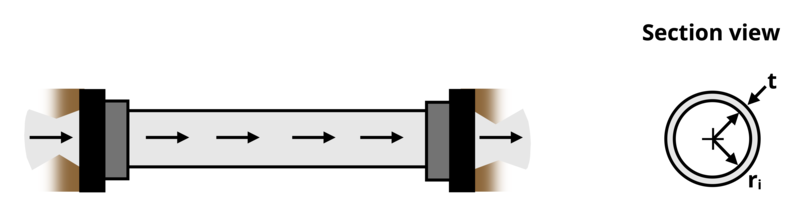
\includegraphics[keepaspectratio]{images/229.png}}
{[}Problem adapted from © Kurt Gramoll CC BY NC-SA 4.0{]}

\begin{Shaded}
\begin{Highlighting}[]
\NormalTok{\#| standalone: true}
\NormalTok{\#| viewerHeight: 600}
\NormalTok{\#| components: [viewer]}

\NormalTok{from shiny import App, render, ui, reactive}
\NormalTok{import random}
\NormalTok{import asyncio}
\NormalTok{import math}
\NormalTok{import io}
\NormalTok{import string}
\NormalTok{from datetime import datetime}
\NormalTok{from pathlib import Path}

\NormalTok{def generate\_random\_letters(length):}
\NormalTok{    \# Generate a random string of letters of specified length}
\NormalTok{    return \textquotesingle{}\textquotesingle{}.join(random.choice(string.ascii\_lowercase) for \_ in range(length))}

\NormalTok{problem\_ID="229"}
\NormalTok{ri=reactive.Value("\_\_")}
\NormalTok{t=reactive.Value("\_\_")}
\NormalTok{T1=reactive.Value("\_\_")}
\NormalTok{T2=reactive.Value("\_\_")}
\NormalTok{L=reactive.Value("\_\_")}
  
\NormalTok{attempts=["Timestamp,Attempt,Answer,Feedback\textbackslash{}n"]}

\NormalTok{app\_ui = ui.page\_fluid(}
\NormalTok{    \#ui.markdown("**Please enter your ID number from your instructor and click to generate your problem**"),}
\NormalTok{    \#ui.input\_text("ID","", placeholder="Enter ID Number Here"),}
\NormalTok{    \#ui.input\_action\_button("generate\_problem", "Generate Problem", class\_="btn{-}primary"),}
\NormalTok{    ui.markdown("**Problem Statement**"),}
\NormalTok{    ui.output\_ui("ui\_problem\_statement"),}
\NormalTok{    ui.input\_text("answer","Your Answer in units of kN", placeholder="Please enter your answer"),}
\NormalTok{    ui.input\_action\_button("submit", "Check Answer", class\_="btn{-}primary"),}
\NormalTok{    \#ui.download\_button("download", "Download File to Submit", class\_="btn{-}success"),}
\NormalTok{)}

\NormalTok{def server(input, output, session):}
\NormalTok{    \# Initialize a counter for attempts}
\NormalTok{    attempt\_counter = reactive.Value(0)}

\NormalTok{    @output}
\NormalTok{    @render.ui}
\NormalTok{    def ui\_problem\_statement():}
\NormalTok{        randomize\_vars()}
\NormalTok{        return[ui.markdown(f"A long steel pipe of length L = \{L()\} m, with an internal radius r\textless{}sub\textgreater{}i\textless{}/sub\textgreater{} = \{ri()\} mm and wall thickness t = \{t()\} mm, is mounted between two fixed walls. Fluid flowing through the pipe raises the temperature from T\textless{}sub\textgreater{}1\textless{}/sub\textgreater{} = \{T1()\}°C to T\textless{}sub\textgreater{}2\textless{}/sub\textgreater{} = \{T2()\}°C. Determine the force on the support due to this heating. Assume E = 20 GPa and α = 12 x 10\textless{}sup\textgreater{}{-}6\textless{}/sup\textgreater{} /°C.")]}
    
\NormalTok{    \#@reactive.Effect}
\NormalTok{    \#@reactive.event(input.generate\_problem)}
\NormalTok{    def randomize\_vars():}
\NormalTok{        random.seed(101)}
\NormalTok{        ri.set(random.randrange(50,150,1))}
\NormalTok{        t.set(random.randrange(10,20,1))}
\NormalTok{        T1.set(random.randrange(20,50,1))}
\NormalTok{        T2.set(random.randrange(150,250,1))}
\NormalTok{        L.set(random.randrange(1,5,0.1))}
        
\NormalTok{    @reactive.Effect}
\NormalTok{    @reactive.event(input.submit)}
\NormalTok{    def \_():}
\NormalTok{        attempt\_counter.set(attempt\_counter() + 1)  \# Increment the attempt counter on each submission.}
\NormalTok{        A = math.pi*((ri()+t())**2{-}(ri())**2)}
\NormalTok{        instr = 12*10**({-}6)*(T2(){-}T1())*A*20}
\NormalTok{        if math.isclose(float(input.answer()), instr, rel\_tol=0.01):}
\NormalTok{            check = "*Correct*"}
\NormalTok{            correct\_indicator = "JL"}
\NormalTok{        else:}
\NormalTok{            check = "*Not Correct.*"}
\NormalTok{            correct\_indicator = "JG"}

\NormalTok{        \# Generate random parts for the encoded attempt.}
\NormalTok{        random\_start = generate\_random\_letters(4)}
\NormalTok{        random\_middle = generate\_random\_letters(4)}
\NormalTok{        random\_end = generate\_random\_letters(4)}
\NormalTok{        \#encoded\_attempt = f"\{random\_start\}\{problem\_ID\}{-}\{random\_middle\}\{attempt\_counter()\}\{correct\_indicator\}{-}\{random\_end\}\{input.ID()\}"}

\NormalTok{        \# Store the most recent encoded attempt in a reactive value so it persists across submissions}
\NormalTok{        \#session.encoded\_attempt = reactive.Value(encoded\_attempt)}

\NormalTok{        \# Append the attempt data to the attempts list without the encoded attempt}
\NormalTok{        attempts.append(f"\{datetime.now()\}, \{attempt\_counter()\}, \{input.answer()\}, \{check\}\textbackslash{}n")}

\NormalTok{        \# Show feedback to the user.}
\NormalTok{        feedback = ui.markdown(f"Your answer of \{input.answer()\} is \{check\}.")}
\NormalTok{        m = ui.modal(}
\NormalTok{            feedback,}
\NormalTok{            title="Feedback",}
\NormalTok{            easy\_close=True}
\NormalTok{        )}
\NormalTok{        ui.modal\_show(m)}

\NormalTok{    \#@render.download(filename=lambda: f"Problem\_Log{-}\{problem\_ID\}{-}\{input.ID()\}.csv")}
\NormalTok{    async def download():}
\NormalTok{        \# Start the CSV with the encoded attempt (without label)}
\NormalTok{        final\_encoded = session.encoded\_attempt() if session.encoded\_attempt is not None else "No attempts"}
\NormalTok{        yield f"\{final\_encoded\}\textbackslash{}n\textbackslash{}n"}
        
\NormalTok{        \# Write the header for the remaining CSV data once}
\NormalTok{        yield "Timestamp,Attempt,Answer,Feedback\textbackslash{}n"}
        
\NormalTok{        \# Write the attempts data, ensure that the header from the attempts list is not written again}
\NormalTok{        for attempt in attempts[1:]:  \# Skip the first element which is the header}
\NormalTok{            await asyncio.sleep(0.25)  \# This delay may not be necessary; adjust as needed}
\NormalTok{            yield attempt}

\NormalTok{\# App installation}
\NormalTok{app = App(app\_ui, server)}
\end{Highlighting}
\end{Shaded}

\chapter*{Problem 5.59 - Thermal
Deformation}\label{problem-5.59---thermal-deformation}
\addcontentsline{toc}{chapter}{Problem 5.59 - Thermal Deformation}

\markboth{Problem 5.59 - Thermal Deformation}{Problem 5.59 - Thermal
Deformation}

\pandocbounded{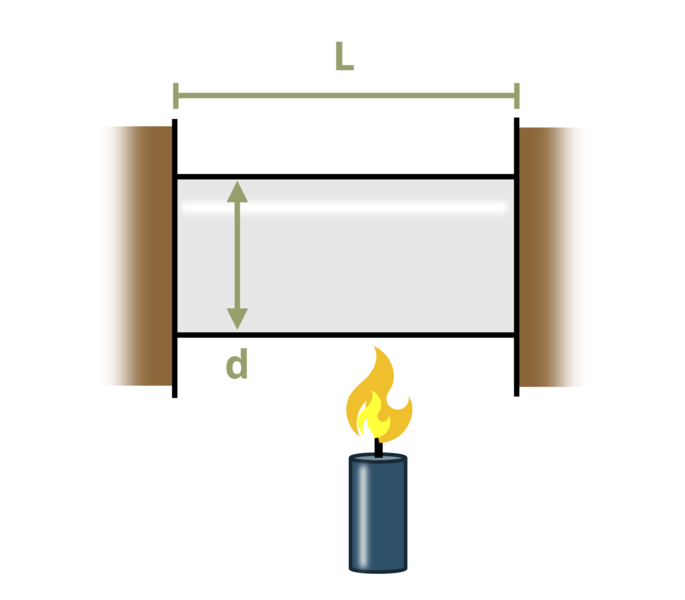
\includegraphics[keepaspectratio]{images/230.png}}
{[}Problem adapted from © Kurt Gramoll CC BY NC-SA 4.0{]}

\begin{Shaded}
\begin{Highlighting}[]
\NormalTok{\#| standalone: true}
\NormalTok{\#| viewerHeight: 600}
\NormalTok{\#| components: [viewer]}

\NormalTok{from shiny import App, render, ui, reactive}
\NormalTok{import random}
\NormalTok{import asyncio}
\NormalTok{import math}
\NormalTok{import io}
\NormalTok{import string}
\NormalTok{from datetime import datetime}
\NormalTok{from pathlib import Path}

\NormalTok{def generate\_random\_letters(length):}
\NormalTok{    \# Generate a random string of letters of specified length}
\NormalTok{    return \textquotesingle{}\textquotesingle{}.join(random.choice(string.ascii\_lowercase) for \_ in range(length))}

\NormalTok{problem\_ID="230"}
\NormalTok{L=reactive.Value("\_\_")}
\NormalTok{d=reactive.Value("\_\_")}
\NormalTok{T1=reactive.Value("\_\_")}
\NormalTok{T2=reactive.Value("\_\_")}
  
\NormalTok{attempts=["Timestamp,Attempt,Answer,Feedback\textbackslash{}n"]}

\NormalTok{app\_ui = ui.page\_fluid(}
\NormalTok{    \#ui.markdown("**Please enter your ID number from your instructor and click to generate your problem**"),}
\NormalTok{    \#ui.input\_text("ID","", placeholder="Enter ID Number Here"),}
\NormalTok{    \#ui.input\_action\_button("generate\_problem", "Generate Problem", class\_="btn{-}primary"),}
\NormalTok{    ui.markdown("**Problem Statement**"),}
\NormalTok{    ui.output\_ui("ui\_problem\_statement"),}
\NormalTok{    ui.input\_text("answer","Your Answer in units of kip", placeholder="Please enter your answer"),}
\NormalTok{    ui.input\_action\_button("submit", "Check Answer", class\_="btn{-}primary"),}
\NormalTok{    \#ui.download\_button("download", "Download File to Submit", class\_="btn{-}success"),}
\NormalTok{)}

\NormalTok{def server(input, output, session):}
\NormalTok{    \# Initialize a counter for attempts}
\NormalTok{    attempt\_counter = reactive.Value(0)}

\NormalTok{    @output}
\NormalTok{    @render.ui}
\NormalTok{    def ui\_problem\_statement():}
\NormalTok{        randomize\_vars()}
\NormalTok{        return[ui.markdown(f"An aluminum cylinder of length L = \{L()\} in. and diameter d = \{d()\} in. is fixed between two walls and heated from T\textless{}sub\textgreater{}1\textless{}/sub\textgreater{} = \{T1()\}°F to T\textless{}sub\textgreater{}2\textless{}/sub\textgreater{} =\{T2()\}°F. Determine the magnitude of the force that the walls exert on the cylinder. Assume α = 13 x 10\textless{}sup\textgreater{}{-}6\textless{}/sup\textgreater{} /°F and E = 10 x 10\textless{}sup\textgreater{}6\textless{}/sup\textgreater{} psi.")]}
    
\NormalTok{    \#@reactive.Effect}
\NormalTok{    \#@reactive.event(input.generate\_problem)}
\NormalTok{    def randomize\_vars():}
\NormalTok{        random.seed(101)}
\NormalTok{        L.set(random.randrange(5,20,1))}
\NormalTok{        d.set(random.randrange(15,50,1)/10)}
\NormalTok{        T1.set(random.randrange(20,50,1))}
\NormalTok{        T2.set(T1()+random.randrange(30,100,1))}
        
\NormalTok{    @reactive.Effect}
\NormalTok{    @reactive.event(input.submit)}
\NormalTok{    def \_():}
\NormalTok{        attempt\_counter.set(attempt\_counter() + 1)  \# Increment the attempt counter on each submission.}
\NormalTok{        delT = 13*10**({-}6)*(T2(){-}T1())*L()}
\NormalTok{        instr = delT*(math.pi*(d()/2)**2)*10*10**6/L()/1000}
\NormalTok{        if math.isclose(float(input.answer()), instr, rel\_tol=0.01):}
\NormalTok{            check = "*Correct*"}
\NormalTok{            correct\_indicator = "JL"}
\NormalTok{        else:}
\NormalTok{            check = "*Not Correct.*"}
\NormalTok{            correct\_indicator = "JG"}

\NormalTok{        \# Generate random parts for the encoded attempt.}
\NormalTok{        random\_start = generate\_random\_letters(4)}
\NormalTok{        random\_middle = generate\_random\_letters(4)}
\NormalTok{        random\_end = generate\_random\_letters(4)}
\NormalTok{        \#encoded\_attempt = f"\{random\_start\}\{problem\_ID\}{-}\{random\_middle\}\{attempt\_counter()\}\{correct\_indicator\}{-}\{random\_end\}\{input.ID()\}"}

\NormalTok{        \# Store the most recent encoded attempt in a reactive value so it persists across submissions}
\NormalTok{        \#session.encoded\_attempt = reactive.Value(encoded\_attempt)}

\NormalTok{        \# Append the attempt data to the attempts list without the encoded attempt}
\NormalTok{        attempts.append(f"\{datetime.now()\}, \{attempt\_counter()\}, \{input.answer()\}, \{check\}\textbackslash{}n")}

\NormalTok{        \# Show feedback to the user.}
\NormalTok{        feedback = ui.markdown(f"Your answer of \{input.answer()\} is \{check\}.")}
\NormalTok{        m = ui.modal(}
\NormalTok{            feedback,}
\NormalTok{            title="Feedback",}
\NormalTok{            easy\_close=True}
\NormalTok{        )}
\NormalTok{        ui.modal\_show(m)}

\NormalTok{    \#@render.download(filename=lambda: f"Problem\_Log{-}\{problem\_ID\}{-}\{input.ID()\}.csv")}
\NormalTok{    async def download():}
\NormalTok{        \# Start the CSV with the encoded attempt (without label)}
\NormalTok{        final\_encoded = session.encoded\_attempt() if session.encoded\_attempt is not None else "No attempts"}
\NormalTok{        yield f"\{final\_encoded\}\textbackslash{}n\textbackslash{}n"}
        
\NormalTok{        \# Write the header for the remaining CSV data once}
\NormalTok{        yield "Timestamp,Attempt,Answer,Feedback\textbackslash{}n"}
        
\NormalTok{        \# Write the attempts data, ensure that the header from the attempts list is not written again}
\NormalTok{        for attempt in attempts[1:]:  \# Skip the first element which is the header}
\NormalTok{            await asyncio.sleep(0.25)  \# This delay may not be necessary; adjust as needed}
\NormalTok{            yield attempt}

\NormalTok{\# App installation}
\NormalTok{app = App(app\_ui, server)}
\end{Highlighting}
\end{Shaded}

\chapter*{Problem 5.60 - Thermal
Deformation}\label{problem-5.60---thermal-deformation}
\addcontentsline{toc}{chapter}{Problem 5.60 - Thermal Deformation}

\markboth{Problem 5.60 - Thermal Deformation}{Problem 5.60 - Thermal
Deformation}

\pandocbounded{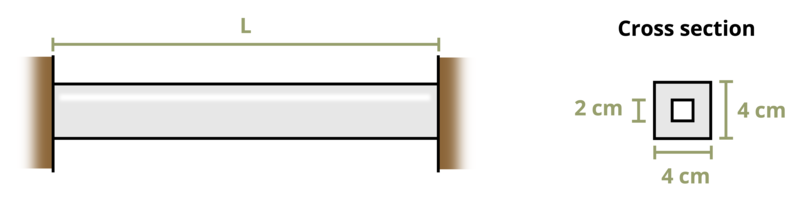
\includegraphics[keepaspectratio]{images/231.png}}
{[}Problem adapted from © Kurt Gramoll CC BY NC-SA 4.0{]}

\begin{Shaded}
\begin{Highlighting}[]
\NormalTok{\#| standalone: true}
\NormalTok{\#| viewerHeight: 600}
\NormalTok{\#| components: [viewer]}

\NormalTok{from shiny import App, render, ui, reactive}
\NormalTok{import random}
\NormalTok{import asyncio}
\NormalTok{import math}
\NormalTok{import io}
\NormalTok{import string}
\NormalTok{from datetime import datetime}
\NormalTok{from pathlib import Path}

\NormalTok{def generate\_random\_letters(length):}
\NormalTok{    \# Generate a random string of letters of specified length}
\NormalTok{    return \textquotesingle{}\textquotesingle{}.join(random.choice(string.ascii\_lowercase) for \_ in range(length))}

\NormalTok{problem\_ID="231"}
\NormalTok{L=reactive.Value("\_\_")}
\NormalTok{T1=reactive.Value("\_\_")}
\NormalTok{T2=reactive.Value("\_\_")}
  
\NormalTok{attempts=["Timestamp,Attempt,Answer,Feedback\textbackslash{}n"]}

\NormalTok{app\_ui = ui.page\_fluid(}
\NormalTok{    \#ui.markdown("**Please enter your ID number from your instructor and click to generate your problem**"),}
\NormalTok{    \#ui.input\_text("ID","", placeholder="Enter ID Number Here"),}
\NormalTok{    \#ui.input\_action\_button("generate\_problem", "Generate Problem", class\_="btn{-}primary"),}
\NormalTok{    ui.markdown("**Problem Statement**"),}
\NormalTok{    ui.output\_ui("ui\_problem\_statement"),}
\NormalTok{    ui.input\_text("answer","Your Answer in units of MPa", placeholder="Please enter your answer"),}
\NormalTok{    ui.input\_action\_button("submit", "Check Answer", class\_="btn{-}primary"),}
\NormalTok{    \#ui.download\_button("download", "Download File to Submit", class\_="btn{-}success"),}
\NormalTok{)}

\NormalTok{def server(input, output, session):}
\NormalTok{    \# Initialize a counter for attempts}
\NormalTok{    attempt\_counter = reactive.Value(0)}

\NormalTok{    @output}
\NormalTok{    @render.ui}
\NormalTok{    def ui\_problem\_statement():}
\NormalTok{        randomize\_vars()}
\NormalTok{        return[ui.markdown(f"A square PVC plastic rod of length L = \{L()\} mm is placed between two fixed walls and heated from T\textless{}sub\textgreater{}1\textless{}/sub\textgreater{} = \{T1()\}°C to T\textless{}sub\textgreater{}2\textless{}/sub\textgreater{} = \{T2()\}°C. Determine the stress created in the bar. Assume E = 2.8 GPa and α = 50 x 10\textless{}sup\textgreater{}{-}6\textless{}/sup\textgreater{} /°C.")]}
    
\NormalTok{    \#@reactive.Effect}
\NormalTok{    \#@reactive.event(input.generate\_problem)}
\NormalTok{    def randomize\_vars():}
\NormalTok{        random.seed(101)}
\NormalTok{        L.set(random.randrange(500,1500,10))}
\NormalTok{        T1.set(random.randrange(0,30,1))}
\NormalTok{        T2.set(T1()+random.randrange(80,150,1))}
        
\NormalTok{    @reactive.Effect}
\NormalTok{    @reactive.event(input.submit)}
\NormalTok{    def \_():}
\NormalTok{        attempt\_counter.set(attempt\_counter() + 1)  \# Increment the attempt counter on each submission.}
\NormalTok{        instr = 2800*50*10**({-}6)*(T2(){-}T1())}
\NormalTok{        if math.isclose(float(input.answer()), instr, rel\_tol=0.01):}
\NormalTok{            check = "*Correct*"}
\NormalTok{            correct\_indicator = "JL"}
\NormalTok{        else:}
\NormalTok{            check = "*Not Correct.*"}
\NormalTok{            correct\_indicator = "JG"}

\NormalTok{        \# Generate random parts for the encoded attempt.}
\NormalTok{        random\_start = generate\_random\_letters(4)}
\NormalTok{        random\_middle = generate\_random\_letters(4)}
\NormalTok{        random\_end = generate\_random\_letters(4)}
\NormalTok{        \#encoded\_attempt = f"\{random\_start\}\{problem\_ID\}{-}\{random\_middle\}\{attempt\_counter()\}\{correct\_indicator\}{-}\{random\_end\}\{input.ID()\}"}

\NormalTok{        \# Store the most recent encoded attempt in a reactive value so it persists across submissions}
\NormalTok{        \#session.encoded\_attempt = reactive.Value(encoded\_attempt)}

\NormalTok{        \# Append the attempt data to the attempts list without the encoded attempt}
\NormalTok{        attempts.append(f"\{datetime.now()\}, \{attempt\_counter()\}, \{input.answer()\}, \{check\}\textbackslash{}n")}

\NormalTok{        \# Show feedback to the user.}
\NormalTok{        feedback = ui.markdown(f"Your answer of \{input.answer()\} is \{check\}.")}
\NormalTok{        m = ui.modal(}
\NormalTok{            feedback,}
\NormalTok{            title="Feedback",}
\NormalTok{            easy\_close=True}
\NormalTok{        )}
\NormalTok{        ui.modal\_show(m)}

\NormalTok{    \#@render.download(filename=lambda: f"Problem\_Log{-}\{problem\_ID\}{-}\{input.ID()\}.csv")}
\NormalTok{    async def download():}
\NormalTok{        \# Start the CSV with the encoded attempt (without label)}
\NormalTok{        final\_encoded = session.encoded\_attempt() if session.encoded\_attempt is not None else "No attempts"}
\NormalTok{        yield f"\{final\_encoded\}\textbackslash{}n\textbackslash{}n"}
        
\NormalTok{        \# Write the header for the remaining CSV data once}
\NormalTok{        yield "Timestamp,Attempt,Answer,Feedback\textbackslash{}n"}
        
\NormalTok{        \# Write the attempts data, ensure that the header from the attempts list is not written again}
\NormalTok{        for attempt in attempts[1:]:  \# Skip the first element which is the header}
\NormalTok{            await asyncio.sleep(0.25)  \# This delay may not be necessary; adjust as needed}
\NormalTok{            yield attempt}

\NormalTok{\# App installation}
\NormalTok{app = App(app\_ui, server)}
\end{Highlighting}
\end{Shaded}

\chapter*{Problem 5.61 - Thermal
Deformation}\label{problem-5.61---thermal-deformation}
\addcontentsline{toc}{chapter}{Problem 5.61 - Thermal Deformation}

\markboth{Problem 5.61 - Thermal Deformation}{Problem 5.61 - Thermal
Deformation}

\pandocbounded{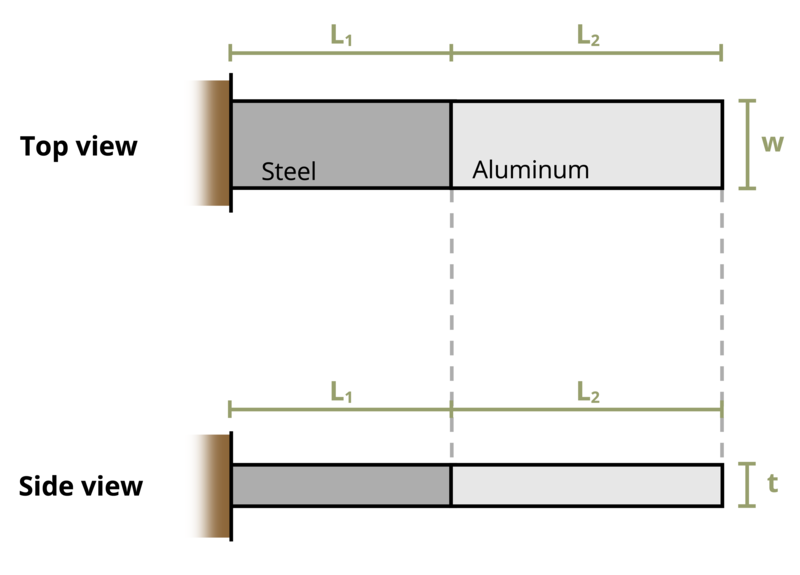
\includegraphics[keepaspectratio]{images/232.png}}
{[}Problem adapted from © Kurt Gramoll CC BY NC-SA 4.0{]}

\begin{Shaded}
\begin{Highlighting}[]
\NormalTok{\#| standalone: true}
\NormalTok{\#| viewerHeight: 600}
\NormalTok{\#| components: [viewer]}

\NormalTok{from shiny import App, render, ui, reactive}
\NormalTok{import random}
\NormalTok{import asyncio}
\NormalTok{import math}
\NormalTok{import io}
\NormalTok{import string}
\NormalTok{from datetime import datetime}
\NormalTok{from pathlib import Path}

\NormalTok{def generate\_random\_letters(length):}
\NormalTok{    \# Generate a random string of letters of specified length}
\NormalTok{    return \textquotesingle{}\textquotesingle{}.join(random.choice(string.ascii\_lowercase) for \_ in range(length))}

\NormalTok{problem\_ID="232"}
\NormalTok{L1=reactive.Value("\_\_")}
\NormalTok{L2=reactive.Value("\_\_")}
\NormalTok{delT=reactive.Value("\_\_")}
\NormalTok{t=reactive.Value("\_\_")}
\NormalTok{w=reactive.Value("\_\_")}

\NormalTok{attempts=["Timestamp,Attempt,Answer,Feedback\textbackslash{}n"]}

\NormalTok{app\_ui = ui.page\_fluid(}
\NormalTok{    \#ui.markdown("**Please enter your ID number from your instructor and click to generate your problem**"),}
\NormalTok{    \#ui.input\_text("ID","", placeholder="Enter ID Number Here"),}
\NormalTok{    \#ui.input\_action\_button("generate\_problem", "Generate Problem", class\_="btn{-}primary"),}
\NormalTok{    ui.markdown("**Problem Statement**"),}
\NormalTok{    ui.output\_ui("ui\_problem\_statement"),}
\NormalTok{    ui.input\_text("answer","Your Answer in units of in", placeholder="Please enter your answer"),}
\NormalTok{    ui.input\_action\_button("submit", "Check Answer", class\_="btn{-}primary"),}
\NormalTok{    \#ui.download\_button("download", "Download File to Submit", class\_="btn{-}success"),}
\NormalTok{)}

\NormalTok{def server(input, output, session):}
\NormalTok{    \# Initialize a counter for attempts}
\NormalTok{    attempt\_counter = reactive.Value(0)}

\NormalTok{    @output}
\NormalTok{    @render.ui}
\NormalTok{    def ui\_problem\_statement():}
\NormalTok{        randomize\_vars()}
\NormalTok{        return[ui.markdown(f"Two solid bars of length L\textless{}sub\textgreater{}1\textless{}/sub\textgreater{} = \{L1()\} in. and L\textless{}sub\textgreater{}2\textless{}/sub\textgreater{} = \{L2()\} in. are heated by ΔT = \{delT()\}°F. The bars have width w = \{w()\} in. and thickness t = \{t()\} in. Determine the total combined change in length of the bars. Assume α\textless{}sub\textgreater{}alum\textless{}/sub\textgreater{} = 13 x 10\textless{}sup\textgreater{}{-}6\textless{}/sup\textgreater{} /°F and α\textless{}sub\textgreater{}steel\textless{}/sub\textgreater{} = 6.5 x 10\textless{}sup\textgreater{}{-}6\textless{}/sup\textgreater{} /°F.")]}
    
\NormalTok{    \#@reactive.Effect}
\NormalTok{    \#@reactive.event(input.generate\_problem)}
\NormalTok{    def randomize\_vars():}
\NormalTok{        random.seed(101)}
\NormalTok{        L1.set(random.randrange(50,100,1)/10)}
\NormalTok{        L2.set(L1()+random.randrange(20,50,1)/10)}
\NormalTok{        delT.set(random.randrange(100,300,1))}
\NormalTok{        t.set(random.randrange(10,20,1)/10)}
\NormalTok{        w.set(t()*2)}
        
\NormalTok{    @reactive.Effect}
\NormalTok{    @reactive.event(input.submit)}
\NormalTok{    def \_():}
\NormalTok{        attempt\_counter.set(attempt\_counter() + 1)  \# Increment the attempt counter on each submission.}
\NormalTok{        instr = (L1()*6.5*10**{-}6+L2()*13*10**{-}6)*delT()}
\NormalTok{        if math.isclose(float(input.answer()), instr, rel\_tol=0.01):}
\NormalTok{            check = "*Correct*"}
\NormalTok{            correct\_indicator = "JL"}
\NormalTok{        else:}
\NormalTok{            check = "*Not Correct.*"}
\NormalTok{            correct\_indicator = "JG"}

\NormalTok{        \# Generate random parts for the encoded attempt.}
\NormalTok{        random\_start = generate\_random\_letters(4)}
\NormalTok{        random\_middle = generate\_random\_letters(4)}
\NormalTok{        random\_end = generate\_random\_letters(4)}
\NormalTok{        \#encoded\_attempt = f"\{random\_start\}\{problem\_ID\}{-}\{random\_middle\}\{attempt\_counter()\}\{correct\_indicator\}{-}\{random\_end\}\{input.ID()\}"}

\NormalTok{        \# Store the most recent encoded attempt in a reactive value so it persists across submissions}
\NormalTok{        \#session.encoded\_attempt = reactive.Value(encoded\_attempt)}

\NormalTok{        \# Append the attempt data to the attempts list without the encoded attempt}
\NormalTok{        attempts.append(f"\{datetime.now()\}, \{attempt\_counter()\}, \{input.answer()\}, \{check\}\textbackslash{}n")}

\NormalTok{        \# Show feedback to the user.}
\NormalTok{        feedback = ui.markdown(f"Your answer of \{input.answer()\} is \{check\}.")}
\NormalTok{        m = ui.modal(}
\NormalTok{            feedback,}
\NormalTok{            title="Feedback",}
\NormalTok{            easy\_close=True}
\NormalTok{        )}
\NormalTok{        ui.modal\_show(m)}

\NormalTok{    \#@render.download(filename=lambda: f"Problem\_Log{-}\{problem\_ID\}{-}\{input.ID()\}.csv")}
\NormalTok{    async def download():}
\NormalTok{        \# Start the CSV with the encoded attempt (without label)}
\NormalTok{        final\_encoded = session.encoded\_attempt() if session.encoded\_attempt is not None else "No attempts"}
\NormalTok{        yield f"\{final\_encoded\}\textbackslash{}n\textbackslash{}n"}
        
\NormalTok{        \# Write the header for the remaining CSV data once}
\NormalTok{        yield "Timestamp,Attempt,Answer,Feedback\textbackslash{}n"}
        
\NormalTok{        \# Write the attempts data, ensure that the header from the attempts list is not written again}
\NormalTok{        for attempt in attempts[1:]:  \# Skip the first element which is the header}
\NormalTok{            await asyncio.sleep(0.25)  \# This delay may not be necessary; adjust as needed}
\NormalTok{            yield attempt}

\NormalTok{\# App installation}
\NormalTok{app = App(app\_ui, server)}
\end{Highlighting}
\end{Shaded}

\chapter*{Problem 5.62 - Thermal
Deformation}\label{problem-5.62---thermal-deformation}
\addcontentsline{toc}{chapter}{Problem 5.62 - Thermal Deformation}

\markboth{Problem 5.62 - Thermal Deformation}{Problem 5.62 - Thermal
Deformation}

\pandocbounded{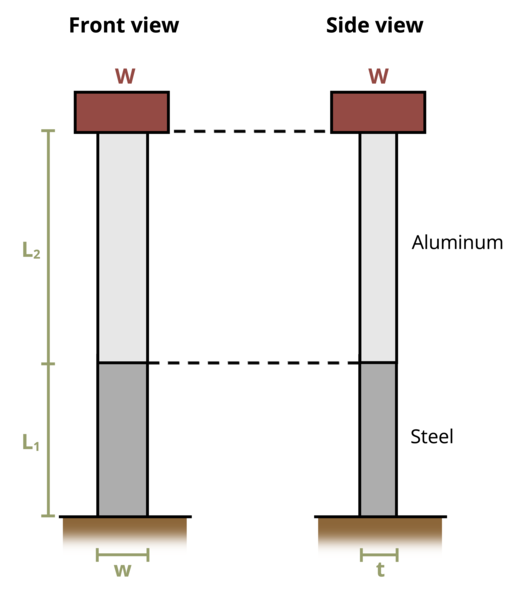
\includegraphics[keepaspectratio]{images/233.png}}
{[}Problem adapted from © Kurt Gramoll CC BY NC-SA 4.0{]}

\begin{Shaded}
\begin{Highlighting}[]
\NormalTok{\#| standalone: true}
\NormalTok{\#| viewerHeight: 600}
\NormalTok{\#| components: [viewer]}

\NormalTok{from shiny import App, render, ui, reactive}
\NormalTok{import random}
\NormalTok{import asyncio}
\NormalTok{import math}
\NormalTok{import io}
\NormalTok{import string}
\NormalTok{from datetime import datetime}
\NormalTok{from pathlib import Path}

\NormalTok{def generate\_random\_letters(length):}
\NormalTok{    \# Generate a random string of letters of specified length}
\NormalTok{    return \textquotesingle{}\textquotesingle{}.join(random.choice(string.ascii\_lowercase) for \_ in range(length))}

\NormalTok{problem\_ID="233"}
\NormalTok{L1=reactive.Value("\_\_")}
\NormalTok{L2=reactive.Value("\_\_")}
\NormalTok{t=reactive.Value("\_\_")}
\NormalTok{w=reactive.Value("\_\_")}
\NormalTok{delT=reactive.Value("\_\_")}

\NormalTok{attempts=["Timestamp,Attempt,Answer,Feedback\textbackslash{}n"]}

\NormalTok{app\_ui = ui.page\_fluid(}
\NormalTok{    \#ui.markdown("**Please enter your ID number from your instructor and click to generate your problem**"),}
\NormalTok{    \#ui.input\_text("ID","", placeholder="Enter ID Number Here"),}
\NormalTok{    \#ui.input\_action\_button("generate\_problem", "Generate Problem", class\_="btn{-}primary"),}
\NormalTok{    ui.markdown("**Problem Statement**"),}
\NormalTok{    ui.output\_ui("ui\_problem\_statement"),}
\NormalTok{    ui.input\_text("answer","Your Answer in units of kip", placeholder="Please enter your answer"),}
\NormalTok{    ui.input\_action\_button("submit", "Check Answer", class\_="btn{-}primary"),}
\NormalTok{    \#ui.download\_button("download", "Download File to Submit", class\_="btn{-}success"),}
\NormalTok{)}

\NormalTok{def server(input, output, session):}
\NormalTok{    \# Initialize a counter for attempts}
\NormalTok{    attempt\_counter = reactive.Value(0)}

\NormalTok{    @output}
\NormalTok{    @render.ui}
\NormalTok{    def ui\_problem\_statement():}
\NormalTok{        randomize\_vars()}
\NormalTok{        return[ui.markdown(f"Two solid bars of length L\textless{}sub\textgreater{}1\textless{}/sub\textgreater{} = \{L1()\} in. and L\textless{}sub\textgreater{}2\textless{}/sub\textgreater{} = \{L2()\} in. are stacked on top of each other, and a box of weight W is placed on top. The bars have width w = \{w()\} in. and thickness t = \{t()\} in. The bars are heated by ΔT = \{delT()\}°F. Determine the weight of the box if the total deflection of the bars is zero. Assume α\textless{}sub\textgreater{}alum\textless{}/sub\textgreater{} = 13 x 10\textless{}sup\textgreater{}{-}6\textless{}/sup\textgreater{} /°F, α\textless{}sub\textgreater{}steel\textless{}/sub\textgreater{} = 6.5 x 10\textless{}sup\textgreater{}{-}6\textless{}/sup\textgreater{} /°F, E\textless{}sub\textgreater{}alum\textless{}/sub\textgreater{} = 10 x 10\textless{}sup\textgreater{}6\textless{}/sup\textgreater{} psi, and E\textless{}sub\textgreater{}steel\textless{}/sub\textgreater{} = 29 x 10\textless{}sup\textgreater{}6\textless{}/sup\textgreater{} psi.")]}
    
\NormalTok{    \#@reactive.Effect}
\NormalTok{    \#@reactive.event(input.generate\_problem)}
\NormalTok{    def randomize\_vars():}
\NormalTok{        random.seed(101)}
\NormalTok{        L1.set(random.randrange(50,100,1)/10)}
\NormalTok{        L2.set(L1()+random.randrange(20,50,1)/10)}
\NormalTok{        t.set(random.randrange(10,20,1)/10)}
\NormalTok{        w.set(t()*2)}
\NormalTok{        delT.set(random.randrange(50,100,1))}
        
\NormalTok{    @reactive.Effect}
\NormalTok{    @reactive.event(input.submit)}
\NormalTok{    def \_():}
\NormalTok{        attempt\_counter.set(attempt\_counter() + 1)  \# Increment the attempt counter on each submission.}
\NormalTok{        dTherm = L1()*6.5*10**{-}6*delT()+L2()*13*10**{-}6*delT()}
\NormalTok{        dM = (L1()/29000+L2()/10000)/(w()*t())}
\NormalTok{        instr = dTherm/dM}
\NormalTok{        if math.isclose(float(input.answer()), instr, rel\_tol=0.01):}
\NormalTok{            check = "*Correct*"}
\NormalTok{            correct\_indicator = "JL"}
\NormalTok{        else:}
\NormalTok{            check = "*Not Correct.*"}
\NormalTok{            correct\_indicator = "JG"}

\NormalTok{        \# Generate random parts for the encoded attempt.}
\NormalTok{        random\_start = generate\_random\_letters(4)}
\NormalTok{        random\_middle = generate\_random\_letters(4)}
\NormalTok{        random\_end = generate\_random\_letters(4)}
\NormalTok{        \#encoded\_attempt = f"\{random\_start\}\{problem\_ID\}{-}\{random\_middle\}\{attempt\_counter()\}\{correct\_indicator\}{-}\{random\_end\}\{input.ID()\}"}

\NormalTok{        \# Store the most recent encoded attempt in a reactive value so it persists across submissions}
\NormalTok{        \#session.encoded\_attempt = reactive.Value(encoded\_attempt)}

\NormalTok{        \# Append the attempt data to the attempts list without the encoded attempt}
\NormalTok{        attempts.append(f"\{datetime.now()\}, \{attempt\_counter()\}, \{input.answer()\}, \{check\}\textbackslash{}n")}

\NormalTok{        \# Show feedback to the user.}
\NormalTok{        feedback = ui.markdown(f"Your answer of \{input.answer()\} is \{check\}.")}
\NormalTok{        m = ui.modal(}
\NormalTok{            feedback,}
\NormalTok{            title="Feedback",}
\NormalTok{            easy\_close=True}
\NormalTok{        )}
\NormalTok{        ui.modal\_show(m)}

\NormalTok{    \#@render.download(filename=lambda: f"Problem\_Log{-}\{problem\_ID\}{-}\{input.ID()\}.csv")}
\NormalTok{    async def download():}
\NormalTok{        \# Start the CSV with the encoded attempt (without label)}
\NormalTok{        final\_encoded = session.encoded\_attempt() if session.encoded\_attempt is not None else "No attempts"}
\NormalTok{        yield f"\{final\_encoded\}\textbackslash{}n\textbackslash{}n"}
        
\NormalTok{        \# Write the header for the remaining CSV data once}
\NormalTok{        yield "Timestamp,Attempt,Answer,Feedback\textbackslash{}n"}
        
\NormalTok{        \# Write the attempts data, ensure that the header from the attempts list is not written again}
\NormalTok{        for attempt in attempts[1:]:  \# Skip the first element which is the header}
\NormalTok{            await asyncio.sleep(0.25)  \# This delay may not be necessary; adjust as needed}
\NormalTok{            yield attempt}

\NormalTok{\# App installation}
\NormalTok{app = App(app\_ui, server)}
\end{Highlighting}
\end{Shaded}

\chapter*{Problem 5.63 - Thermal
Deformation}\label{problem-5.63---thermal-deformation}
\addcontentsline{toc}{chapter}{Problem 5.63 - Thermal Deformation}

\markboth{Problem 5.63 - Thermal Deformation}{Problem 5.63 - Thermal
Deformation}

\pandocbounded{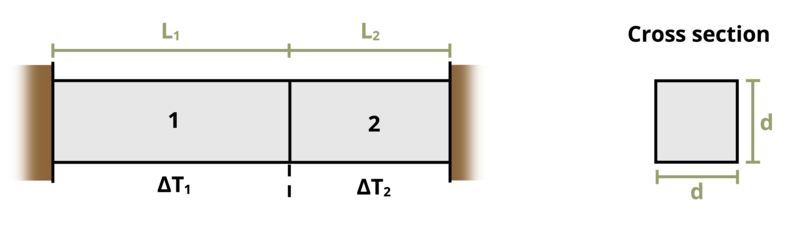
\includegraphics[keepaspectratio]{images/235.png}}
{[}Problem adapted from © Kurt Gramoll CC BY NC-SA 4.0{]}

\begin{Shaded}
\begin{Highlighting}[]
\NormalTok{\#| standalone: true}
\NormalTok{\#| viewerHeight: 600}
\NormalTok{\#| components: [viewer]}

\NormalTok{from shiny import App, render, ui, reactive}
\NormalTok{import random}
\NormalTok{import asyncio}
\NormalTok{import math}
\NormalTok{import io}
\NormalTok{import string}
\NormalTok{from datetime import datetime}
\NormalTok{from pathlib import Path}

\NormalTok{def generate\_random\_letters(length):}
\NormalTok{    \# Generate a random string of letters of specified length}
\NormalTok{    return \textquotesingle{}\textquotesingle{}.join(random.choice(string.ascii\_lowercase) for \_ in range(length))}

\NormalTok{problem\_ID="235"}
\NormalTok{L2=reactive.Value("\_\_")}
\NormalTok{L1=reactive.Value("\_\_")}
\NormalTok{delT1=reactive.Value("\_\_")}
\NormalTok{delT2=reactive.Value("\_\_")}

\NormalTok{attempts=["Timestamp,Attempt,Answer,Feedback\textbackslash{}n"]}

\NormalTok{app\_ui = ui.page\_fluid(}
\NormalTok{    \#ui.markdown("**Please enter your ID number from your instructor and click to generate your problem**"),}
\NormalTok{    \#ui.input\_text("ID","", placeholder="Enter ID Number Here"),}
\NormalTok{    \#ui.input\_action\_button("generate\_problem", "Generate Problem", class\_="btn{-}primary"),}
\NormalTok{    ui.markdown("**Problem Statement**"),}
\NormalTok{    ui.output\_ui("ui\_problem\_statement"),}
\NormalTok{    ui.input\_text("answer","Your Answer in units of ksi", placeholder="Please enter your answer"),}
\NormalTok{    ui.input\_action\_button("submit", "Check Answer", class\_="btn{-}primary"),}
\NormalTok{    \#ui.download\_button("download", "Download File to Submit", class\_="btn{-}success"),}
\NormalTok{)}

\NormalTok{def server(input, output, session):}
\NormalTok{    \# Initialize a counter for attempts}
\NormalTok{    attempt\_counter = reactive.Value(0)}

\NormalTok{    @output}
\NormalTok{    @render.ui}
\NormalTok{    def ui\_problem\_statement():}
\NormalTok{        randomize\_vars()}
\NormalTok{        return[ui.markdown(f"A square steel 1 inch bar is placed between two fixed walls. The bar is heated such that section 1 of length L\textless{}sub\textgreater{}1\textless{}/sub\textgreater{} = \{L1()\} in. is heated by ΔT\textless{}sub\textgreater{}1\textless{}/sub\textgreater{} = \{delT1()\}°F and section 2 of length L\textless{}sub\textgreater{}2\textless{}/sub\textgreater{} = \{L2()\} in. is heated by ΔT\textless{}sub\textgreater{}2\textless{}/sub\textgreater{} = \{delT2()\}°F. Determine the stress created in the bar. Assume E = 29,000 ksi and α = 6.5 x 10\textless{}sup\textgreater{}{-}6\textless{}/sup\textgreater{} /°F.")]}
    
\NormalTok{    \#@reactive.Effect}
\NormalTok{    \#@reactive.event(input.generate\_problem)}
\NormalTok{    def randomize\_vars():}
\NormalTok{        random.seed(101)}
\NormalTok{        L2.set(random.randrange(40,100,1)/10)}
\NormalTok{        L1.set(L2()+random.randrange(20,60,1)/10)}
\NormalTok{        delT1.set(random.randrange(50,100,1))}
\NormalTok{        delT2.set(delT1()+random.randrange(50,100,1))}
        
\NormalTok{    @reactive.Effect}
\NormalTok{    @reactive.event(input.submit)}
\NormalTok{    def \_():}
\NormalTok{        attempt\_counter.set(attempt\_counter() + 1)  \# Increment the attempt counter on each submission.}
\NormalTok{        dTherm = 6.5*10**{-}6*(L1()*delT1()+L2()*delT2())}
\NormalTok{        instr = dTherm*29000/(L1()+L2())}
\NormalTok{        if math.isclose(float(input.answer()), instr, rel\_tol=0.01):}
\NormalTok{            check = "*Correct*"}
\NormalTok{            correct\_indicator = "JL"}
\NormalTok{        else:}
\NormalTok{            check = "*Not Correct.*"}
\NormalTok{            correct\_indicator = "JG"}

\NormalTok{        \# Generate random parts for the encoded attempt.}
\NormalTok{        random\_start = generate\_random\_letters(4)}
\NormalTok{        random\_middle = generate\_random\_letters(4)}
\NormalTok{        random\_end = generate\_random\_letters(4)}
\NormalTok{        \#encoded\_attempt = f"\{random\_start\}\{problem\_ID\}{-}\{random\_middle\}\{attempt\_counter()\}\{correct\_indicator\}{-}\{random\_end\}\{input.ID()\}"}

\NormalTok{        \# Store the most recent encoded attempt in a reactive value so it persists across submissions}
\NormalTok{        \#session.encoded\_attempt = reactive.Value(encoded\_attempt)}

\NormalTok{        \# Append the attempt data to the attempts list without the encoded attempt}
\NormalTok{        attempts.append(f"\{datetime.now()\}, \{attempt\_counter()\}, \{input.answer()\}, \{check\}\textbackslash{}n")}

\NormalTok{        \# Show feedback to the user.}
\NormalTok{        feedback = ui.markdown(f"Your answer of \{input.answer()\} is \{check\}.")}
\NormalTok{        m = ui.modal(}
\NormalTok{            feedback,}
\NormalTok{            title="Feedback",}
\NormalTok{            easy\_close=True}
\NormalTok{        )}
\NormalTok{        ui.modal\_show(m)}

\NormalTok{    \#@render.download(filename=lambda: f"Problem\_Log{-}\{problem\_ID\}{-}\{input.ID()\}.csv")}
\NormalTok{    async def download():}
\NormalTok{        \# Start the CSV with the encoded attempt (without label)}
\NormalTok{        final\_encoded = session.encoded\_attempt() if session.encoded\_attempt is not None else "No attempts"}
\NormalTok{        yield f"\{final\_encoded\}\textbackslash{}n\textbackslash{}n"}
        
\NormalTok{        \# Write the header for the remaining CSV data once}
\NormalTok{        yield "Timestamp,Attempt,Answer,Feedback\textbackslash{}n"}
        
\NormalTok{        \# Write the attempts data, ensure that the header from the attempts list is not written again}
\NormalTok{        for attempt in attempts[1:]:  \# Skip the first element which is the header}
\NormalTok{            await asyncio.sleep(0.25)  \# This delay may not be necessary; adjust as needed}
\NormalTok{            yield attempt}

\NormalTok{\# App installation}
\NormalTok{app = App(app\_ui, server)}
\end{Highlighting}
\end{Shaded}

\chapter*{Problem 5.64 - Thermal
Deformation}\label{problem-5.64---thermal-deformation}
\addcontentsline{toc}{chapter}{Problem 5.64 - Thermal Deformation}

\markboth{Problem 5.64 - Thermal Deformation}{Problem 5.64 - Thermal
Deformation}

\pandocbounded{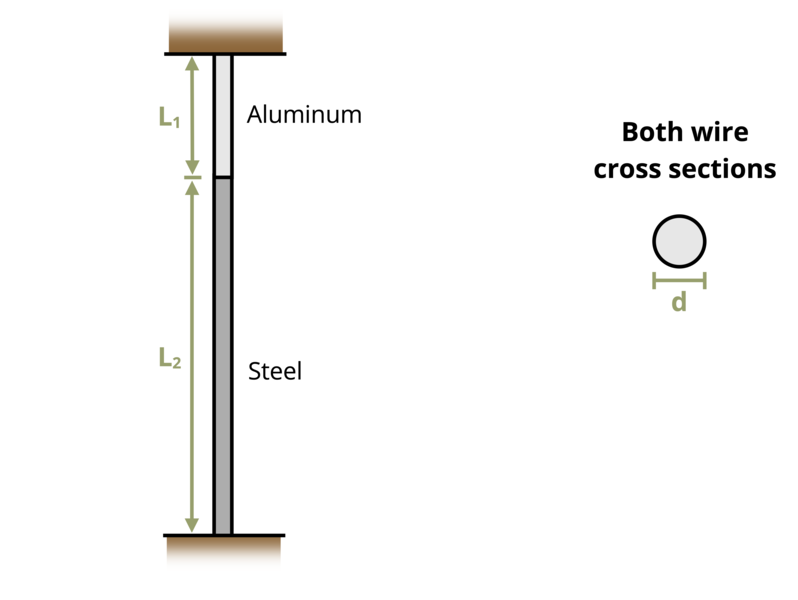
\includegraphics[keepaspectratio]{images/236.png}}
{[}Problem adapted from © Kurt Gramoll CC BY NC-SA 4.0{]}

\begin{Shaded}
\begin{Highlighting}[]
\NormalTok{\#| standalone: true}
\NormalTok{\#| viewerHeight: 600}
\NormalTok{\#| components: [viewer]}

\NormalTok{from shiny import App, render, ui, reactive}
\NormalTok{import random}
\NormalTok{import asyncio}
\NormalTok{import math}
\NormalTok{import io}
\NormalTok{import string}
\NormalTok{from datetime import datetime}
\NormalTok{from pathlib import Path}

\NormalTok{def generate\_random\_letters(length):}
\NormalTok{    \# Generate a random string of letters of specified length}
\NormalTok{    return \textquotesingle{}\textquotesingle{}.join(random.choice(string.ascii\_lowercase) for \_ in range(length))}

\NormalTok{problem\_ID="236"}
\NormalTok{L1=reactive.Value("\_\_")}
\NormalTok{L2=reactive.Value("\_\_")}
\NormalTok{delT=reactive.Value("\_\_")}
\NormalTok{d=reactive.Value("\_\_")}

\NormalTok{attempts=["Timestamp,Attempt,Answer,Feedback\textbackslash{}n"]}

\NormalTok{app\_ui = ui.page\_fluid(}
\NormalTok{    \#ui.markdown("**Please enter your ID number from your instructor and click to generate your problem**"),}
\NormalTok{    \#ui.input\_text("ID","", placeholder="Enter ID Number Here"),}
\NormalTok{    \#ui.input\_action\_button("generate\_problem", "Generate Problem", class\_="btn{-}primary"),}
\NormalTok{    ui.markdown("**Problem Statement**"),}
\NormalTok{    ui.output\_ui("ui\_problem\_statement"),}
\NormalTok{    ui.input\_text("answer","Your Answer in units of MPa", placeholder="Please enter your answer"),}
\NormalTok{    ui.input\_action\_button("submit", "Check Answer", class\_="btn{-}primary"),}
\NormalTok{    \#ui.download\_button("download", "Download File to Submit", class\_="btn{-}success"),}
\NormalTok{)}

\NormalTok{def server(input, output, session):}
\NormalTok{    \# Initialize a counter for attempts}
\NormalTok{    attempt\_counter = reactive.Value(0)}

\NormalTok{    @output}
\NormalTok{    @render.ui}
\NormalTok{    def ui\_problem\_statement():}
\NormalTok{        randomize\_vars()}
\NormalTok{        return[ui.markdown(f"Two wires of length L\textless{}sub\textgreater{}1\textless{}/sub\textgreater{} = \{L1()\} m and L\textless{}sub\textgreater{}2\textless{}/sub\textgreater{} = \{L2()\} m are connected together and attached to the ceiling and floor of a room. If the room is cooled by \{delT()\}°C, dettermine the largest stress in either wire. Assume the diameter d = \{d()\} mm, α\textless{}sub\textgreater{}alum\textless{}/sub\textgreater{} = 23 x 10\textless{}sup\textgreater{}{-}6\textless{}/sup\textgreater{} /°C, E\textless{}sub\textgreater{}alum\textless{}/sub\textgreater{} = 70 GPa, α\textless{}sub\textgreater{}steel\textless{}/sub\textgreater{} = 12 x 10\textless{}sup\textgreater{}{-}6\textless{}/sup\textgreater{} /°C, and E\textless{}sub\textgreater{}steel\textless{}/sub\textgreater{} = 190 GPa.")]}
    
\NormalTok{    \#@reactive.Effect}
\NormalTok{    \#@reactive.event(input.generate\_problem)}
\NormalTok{    def randomize\_vars():}
\NormalTok{        random.seed(101)}
\NormalTok{        L1.set(random.randrange(10,50,1)/10)}
\NormalTok{        L2.set(L1()*3)}
\NormalTok{        delT.set(random.randrange(20,50,1))}
\NormalTok{        d.set(random.randrange(5,10,1))}
        
\NormalTok{    @reactive.Effect}
\NormalTok{    @reactive.event(input.submit)}
\NormalTok{    def \_():}
\NormalTok{        attempt\_counter.set(attempt\_counter() + 1)  \# Increment the attempt counter on each submission.}
\NormalTok{        A = (d()/2)**2*math.pi*10**{-}6}
\NormalTok{        dTherm = 12*10**{-}6*delT()*L2()+23*10**{-}6*delT()*L1()}
\NormalTok{        F = dTherm/(L1()/(70*10**9*A)+L2()/(190*10**9*A))}
\NormalTok{        instr = F/A/10**6}
\NormalTok{        if math.isclose(float(input.answer()), instr, rel\_tol=0.01):}
\NormalTok{            check = "*Correct*"}
\NormalTok{            correct\_indicator = "JL"}
\NormalTok{        else:}
\NormalTok{            check = "*Not Correct.*"}
\NormalTok{            correct\_indicator = "JG"}

\NormalTok{        \# Generate random parts for the encoded attempt.}
\NormalTok{        random\_start = generate\_random\_letters(4)}
\NormalTok{        random\_middle = generate\_random\_letters(4)}
\NormalTok{        random\_end = generate\_random\_letters(4)}
\NormalTok{        \#encoded\_attempt = f"\{random\_start\}\{problem\_ID\}{-}\{random\_middle\}\{attempt\_counter()\}\{correct\_indicator\}{-}\{random\_end\}\{input.ID()\}"}

\NormalTok{        \# Store the most recent encoded attempt in a reactive value so it persists across submissions}
\NormalTok{        \#session.encoded\_attempt = reactive.Value(encoded\_attempt)}

\NormalTok{        \# Append the attempt data to the attempts list without the encoded attempt}
\NormalTok{        attempts.append(f"\{datetime.now()\}, \{attempt\_counter()\}, \{input.answer()\}, \{check\}\textbackslash{}n")}

\NormalTok{        \# Show feedback to the user.}
\NormalTok{        feedback = ui.markdown(f"Your answer of \{input.answer()\} is \{check\}.")}
\NormalTok{        m = ui.modal(}
\NormalTok{            feedback,}
\NormalTok{            title="Feedback",}
\NormalTok{            easy\_close=True}
\NormalTok{        )}
\NormalTok{        ui.modal\_show(m)}

\NormalTok{    \#@render.download(filename=lambda: f"Problem\_Log{-}\{problem\_ID\}{-}\{input.ID()\}.csv")}
\NormalTok{    async def download():}
\NormalTok{        \# Start the CSV with the encoded attempt (without label)}
\NormalTok{        final\_encoded = session.encoded\_attempt() if session.encoded\_attempt is not None else "No attempts"}
\NormalTok{        yield f"\{final\_encoded\}\textbackslash{}n\textbackslash{}n"}
        
\NormalTok{        \# Write the header for the remaining CSV data once}
\NormalTok{        yield "Timestamp,Attempt,Answer,Feedback\textbackslash{}n"}
        
\NormalTok{        \# Write the attempts data, ensure that the header from the attempts list is not written again}
\NormalTok{        for attempt in attempts[1:]:  \# Skip the first element which is the header}
\NormalTok{            await asyncio.sleep(0.25)  \# This delay may not be necessary; adjust as needed}
\NormalTok{            yield attempt}

\NormalTok{\# App installation}
\NormalTok{app = App(app\_ui, server)}
\end{Highlighting}
\end{Shaded}

\chapter*{Problem 5.65 - Thermal
Deformation}\label{problem-5.65---thermal-deformation}
\addcontentsline{toc}{chapter}{Problem 5.65 - Thermal Deformation}

\markboth{Problem 5.65 - Thermal Deformation}{Problem 5.65 - Thermal
Deformation}

\pandocbounded{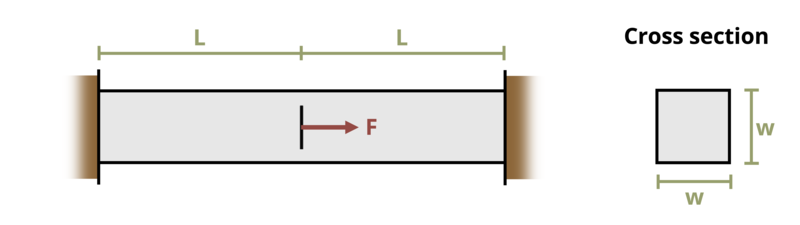
\includegraphics[keepaspectratio]{images/237.png}}
{[}Problem adapted from © Kurt Gramoll CC BY NC-SA 4.0{]}

\begin{Shaded}
\begin{Highlighting}[]
\NormalTok{\#| standalone: true}
\NormalTok{\#| viewerHeight: 600}
\NormalTok{\#| components: [viewer]}

\NormalTok{from shiny import App, render, ui, reactive}
\NormalTok{import random}
\NormalTok{import asyncio}
\NormalTok{import math}
\NormalTok{import io}
\NormalTok{import string}
\NormalTok{from datetime import datetime}
\NormalTok{from pathlib import Path}

\NormalTok{def generate\_random\_letters(length):}
\NormalTok{    \# Generate a random string of letters of specified length}
\NormalTok{    return \textquotesingle{}\textquotesingle{}.join(random.choice(string.ascii\_lowercase) for \_ in range(length))}

\NormalTok{problem\_ID="237"}
\NormalTok{w=reactive.Value("\_\_")}
\NormalTok{delT=reactive.Value("\_\_")}
\NormalTok{F=reactive.Value("\_\_")}
\NormalTok{L=reactive.Value("\_\_")}

\NormalTok{attempts=["Timestamp,Attempt,Answer,Feedback\textbackslash{}n"]}

\NormalTok{app\_ui = ui.page\_fluid(}
\NormalTok{    \#ui.markdown("**Please enter your ID number from your instructor and click to generate your problem**"),}
\NormalTok{    \#ui.input\_text("ID","", placeholder="Enter ID Number Here"),}
\NormalTok{    \#ui.input\_action\_button("generate\_problem", "Generate Problem", class\_="btn{-}primary"),}
\NormalTok{    ui.markdown("**Problem Statement**"),}
\NormalTok{    ui.output\_ui("ui\_problem\_statement"),}
\NormalTok{    ui.input\_text("answer","Your Answer in units of kN", placeholder="Please enter your answer"),}
\NormalTok{    ui.input\_action\_button("submit", "Check Answer", class\_="btn{-}primary"),}
\NormalTok{    \#ui.download\_button("download", "Download File to Submit", class\_="btn{-}success"),}
\NormalTok{)}

\NormalTok{def server(input, output, session):}
\NormalTok{    \# Initialize a counter for attempts}
\NormalTok{    attempt\_counter = reactive.Value(0)}

\NormalTok{    @output}
\NormalTok{    @render.ui}
\NormalTok{    def ui\_problem\_statement():}
\NormalTok{        randomize\_vars()}
\NormalTok{        return[ui.markdown(f"A square steel bar with cross{-}section side length w = \{w()\} mm is placed between two fixed walls. The bar is heated so that the change in temperature ΔT = \{delT()\}°C. A single load F = \{F()\} kN is applied at the center. If length L = \{L()\} m, determine the reaction force on the right wall. Assume E = 200 GPa and α = 12 x 10\textless{}sup\textgreater{}{-}6\textless{}/sup\textgreater{} /°C.")]}
    
\NormalTok{    \#@reactive.Effect}
\NormalTok{    \#@reactive.event(input.generate\_problem)}
\NormalTok{    def randomize\_vars():}
\NormalTok{        random.seed(101)}
\NormalTok{        w.set(random.randrange(10,50,1))}
\NormalTok{        delT.set(random.randrange(250,500,10))}
\NormalTok{        F.set(random.randrange(50,200,1))}
\NormalTok{        L.set(random.randrange(10,50,1)/10)}
        
\NormalTok{    @reactive.Effect}
\NormalTok{    @reactive.event(input.submit)}
\NormalTok{    def \_():}
\NormalTok{        attempt\_counter.set(attempt\_counter() + 1)  \# Increment the attempt counter on each submission.}
\NormalTok{        dTherm = 12*10**{-}6*2*L()*delT()}
\NormalTok{        FLR = dTherm/(L()/(200*10**9*w()*w()*10**{-}6))*10**{-}3}
\NormalTok{        instr = (FLR+F())/2}
\NormalTok{        if math.isclose(float(input.answer()), instr, rel\_tol=0.01):}
\NormalTok{            check = "*Correct*"}
\NormalTok{            correct\_indicator = "JL"}
\NormalTok{        else:}
\NormalTok{            check = "*Not Correct*"}
\NormalTok{            correct\_indicator = "JG"}

\NormalTok{        \# Generate random parts for the encoded attempt.}
\NormalTok{        random\_start = generate\_random\_letters(4)}
\NormalTok{        random\_middle = generate\_random\_letters(4)}
\NormalTok{        random\_end = generate\_random\_letters(4)}
\NormalTok{        \#encoded\_attempt = f"\{random\_start\}\{problem\_ID\}{-}\{random\_middle\}\{attempt\_counter()\}\{correct\_indicator\}{-}\{random\_end\}\{input.ID()\}"}

\NormalTok{        \# Store the most recent encoded attempt in a reactive value so it persists across submissions}
\NormalTok{        \#session.encoded\_attempt = reactive.Value(encoded\_attempt)}

\NormalTok{        \# Append the attempt data to the attempts list without the encoded attempt}
\NormalTok{        attempts.append(f"\{datetime.now()\}, \{attempt\_counter()\}, \{input.answer()\}, \{check\}\textbackslash{}n")}

\NormalTok{        \# Show feedback to the user.}
\NormalTok{        feedback = ui.markdown(f"Your answer of \{input.answer()\} is \{check\}.")}
\NormalTok{        m = ui.modal(}
\NormalTok{            feedback,}
\NormalTok{            title="Feedback",}
\NormalTok{            easy\_close=True}
\NormalTok{        )}
\NormalTok{        ui.modal\_show(m)}

\NormalTok{    \#@render.download(filename=lambda: f"Problem\_Log{-}\{problem\_ID\}{-}\{input.ID()\}.csv")}
\NormalTok{    async def download():}
\NormalTok{        \# Start the CSV with the encoded attempt (without label)}
\NormalTok{        final\_encoded = session.encoded\_attempt() if session.encoded\_attempt is not None else "No attempts"}
\NormalTok{        yield f"\{final\_encoded\}\textbackslash{}n\textbackslash{}n"}
        
\NormalTok{        \# Write the header for the remaining CSV data once}
\NormalTok{        yield "Timestamp,Attempt,Answer,Feedback\textbackslash{}n"}
        
\NormalTok{        \# Write the attempts data, ensure that the header from the attempts list is not written again}
\NormalTok{        for attempt in attempts[1:]:  \# Skip the first element which is the header}
\NormalTok{            await asyncio.sleep(0.25)  \# This delay may not be necessary; adjust as needed}
\NormalTok{            yield attempt}

\NormalTok{\# App installation}
\NormalTok{app = App(app\_ui, server)}
\end{Highlighting}
\end{Shaded}

\chapter*{Problem 5.66 - Thermal
Deformation}\label{problem-5.66---thermal-deformation}
\addcontentsline{toc}{chapter}{Problem 5.66 - Thermal Deformation}

\markboth{Problem 5.66 - Thermal Deformation}{Problem 5.66 - Thermal
Deformation}

\pandocbounded{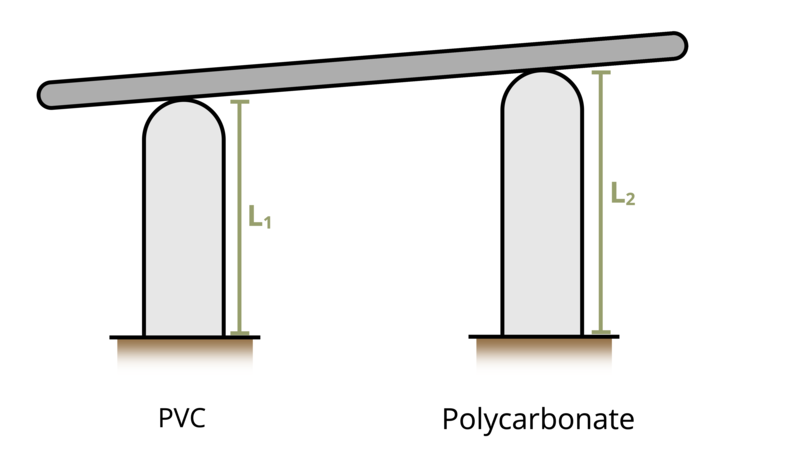
\includegraphics[keepaspectratio]{images/238.png}}
{[}Problem adapted from © Kurt Gramoll CC BY NC-SA 4.0{]}

\begin{Shaded}
\begin{Highlighting}[]
\NormalTok{\#| standalone: true}
\NormalTok{\#| viewerHeight: 600}
\NormalTok{\#| components: [viewer]}

\NormalTok{from shiny import App, render, ui, reactive}
\NormalTok{import random}
\NormalTok{import asyncio}
\NormalTok{import math}
\NormalTok{import io}
\NormalTok{import string}
\NormalTok{from datetime import datetime}
\NormalTok{from pathlib import Path}

\NormalTok{def generate\_random\_letters(length):}
\NormalTok{    \# Generate a random string of letters of specified length}
\NormalTok{    return \textquotesingle{}\textquotesingle{}.join(random.choice(string.ascii\_lowercase) for \_ in range(length))}

\NormalTok{problem\_ID="238"}
\NormalTok{L1=reactive.Value("\_\_")}
\NormalTok{L2=reactive.Value("\_\_")}
\NormalTok{aPVC=reactive.Value("\_\_")}
\NormalTok{aPoly=reactive.Value("\_\_")}

\NormalTok{attempts=["Timestamp,Attempt,Answer,Feedback\textbackslash{}n"]}

\NormalTok{app\_ui = ui.page\_fluid(}
\NormalTok{    \#ui.markdown("**Please enter your ID number from your instructor and click to generate your problem**"),}
\NormalTok{    \#ui.input\_text("ID","", placeholder="Enter ID Number Here"),}
\NormalTok{    \#ui.input\_action\_button("generate\_problem", "Generate Problem", class\_="btn{-}primary"),}
\NormalTok{    ui.markdown("**Problem Statement**"),}
\NormalTok{    ui.output\_ui("ui\_problem\_statement"),}
\NormalTok{    ui.input\_text("answer","Your Answer in units of \textbackslash{}u00b0C", placeholder="Please enter your answer"),}
\NormalTok{    ui.input\_action\_button("submit", "Check Answer", class\_="btn{-}primary"),}
\NormalTok{    \#ui.download\_button("download", "Download File to Submit", class\_="btn{-}success"),}
\NormalTok{)}

\NormalTok{def server(input, output, session):}
\NormalTok{    \# Initialize a counter for attempts}
\NormalTok{    attempt\_counter = reactive.Value(0)}

\NormalTok{    @output}
\NormalTok{    @render.ui}
\NormalTok{    def ui\_problem\_statement():}
\NormalTok{        randomize\_vars()}
\NormalTok{        return[ui.markdown(f"Two posts support a slender bar as shown, where L\textless{}sub\textgreater{}1\textless{}/sub\textgreater{} = \{L1()\} m and L\textless{}sub\textgreater{}2\textless{}/sub\textgreater{} = \{L2()\} m, causing the bar to be at a slight angle. Determine the increase in temperature that will cause the bar to become horizontal. Assume α\textless{}sub\textgreater{}PVC\textless{}/sub\textgreater{} = \{aPVC()\} x 10\textless{}sup\textgreater{}{-}6\textless{}/sup\textgreater{} /°C and α\textless{}sub\textgreater{}poly\textless{}/sub\textgreater{} = \{aPoly()\} x 10\textless{}sup\textgreater{}{-}6\textless{}/sup\textgreater{} /°C. Ignore the weight of the bar.")]}
    
\NormalTok{    \#@reactive.Effect}
\NormalTok{    \#@reactive.event(input.generate\_problem)}
\NormalTok{    def randomize\_vars():}
\NormalTok{        random.seed(101)}
\NormalTok{        L1.set(random.randrange(30,50,1)/1000)}
\NormalTok{        L2.set(L1()+random.randrange(1,3,1)/1000)}
\NormalTok{        aPVC.set(random.randrange(40,60,1))}
\NormalTok{        aPoly.set(random.randrange(60,100,1)/10)}
        
\NormalTok{    @reactive.Effect}
\NormalTok{    @reactive.event(input.submit)}
\NormalTok{    def \_():}
\NormalTok{        attempt\_counter.set(attempt\_counter() + 1)  \# Increment the attempt counter on each submission.}
\NormalTok{        instr = (L2(){-}L1())/(aPVC()*10**{-}6*L1(){-}aPoly()*10**{-}6*L2())}
\NormalTok{        if math.isclose(float(input.answer()), instr, rel\_tol=0.01):}
\NormalTok{            check = "*Correct*"}
\NormalTok{            correct\_indicator = "JL"}
\NormalTok{        else:}
\NormalTok{            check = "*Not Correct*"}
\NormalTok{            correct\_indicator = "JG"}

\NormalTok{        \# Generate random parts for the encoded attempt.}
\NormalTok{        random\_start = generate\_random\_letters(4)}
\NormalTok{        random\_middle = generate\_random\_letters(4)}
\NormalTok{        random\_end = generate\_random\_letters(4)}
\NormalTok{        \#encoded\_attempt = f"\{random\_start\}\{problem\_ID\}{-}\{random\_middle\}\{attempt\_counter()\}\{correct\_indicator\}{-}\{random\_end\}\{input.ID()\}"}

\NormalTok{        \# Store the most recent encoded attempt in a reactive value so it persists across submissions}
\NormalTok{        \#session.encoded\_attempt = reactive.Value(encoded\_attempt)}

\NormalTok{        \# Append the attempt data to the attempts list without the encoded attempt}
\NormalTok{        attempts.append(f"\{datetime.now()\}, \{attempt\_counter()\}, \{input.answer()\}, \{check\}\textbackslash{}n")}

\NormalTok{        \# Show feedback to the user.}
\NormalTok{        feedback = ui.markdown(f"Your answer of \{input.answer()\} is \{check\}.")}
\NormalTok{        m = ui.modal(}
\NormalTok{            feedback,}
\NormalTok{            title="Feedback",}
\NormalTok{            easy\_close=True}
\NormalTok{        )}
\NormalTok{        ui.modal\_show(m)}

\NormalTok{    \#@render.download(filename=lambda: f"Problem\_Log{-}\{problem\_ID\}{-}\{input.ID()\}.csv")}
\NormalTok{    async def download():}
\NormalTok{        \# Start the CSV with the encoded attempt (without label)}
\NormalTok{        final\_encoded = session.encoded\_attempt() if session.encoded\_attempt is not None else "No attempts"}
\NormalTok{        yield f"\{final\_encoded\}\textbackslash{}n\textbackslash{}n"}
        
\NormalTok{        \# Write the header for the remaining CSV data once}
\NormalTok{        yield "Timestamp,Attempt,Answer,Feedback\textbackslash{}n"}
        
\NormalTok{        \# Write the attempts data, ensure that the header from the attempts list is not written again}
\NormalTok{        for attempt in attempts[1:]:  \# Skip the first element which is the header}
\NormalTok{            await asyncio.sleep(0.25)  \# This delay may not be necessary; adjust as needed}
\NormalTok{            yield attempt}

\NormalTok{\# App installation}
\NormalTok{app = App(app\_ui, server)}
\end{Highlighting}
\end{Shaded}

\chapter*{Problem 5.67 - Thermal
Deformation}\label{problem-5.67---thermal-deformation}
\addcontentsline{toc}{chapter}{Problem 5.67 - Thermal Deformation}

\markboth{Problem 5.67 - Thermal Deformation}{Problem 5.67 - Thermal
Deformation}

\pandocbounded{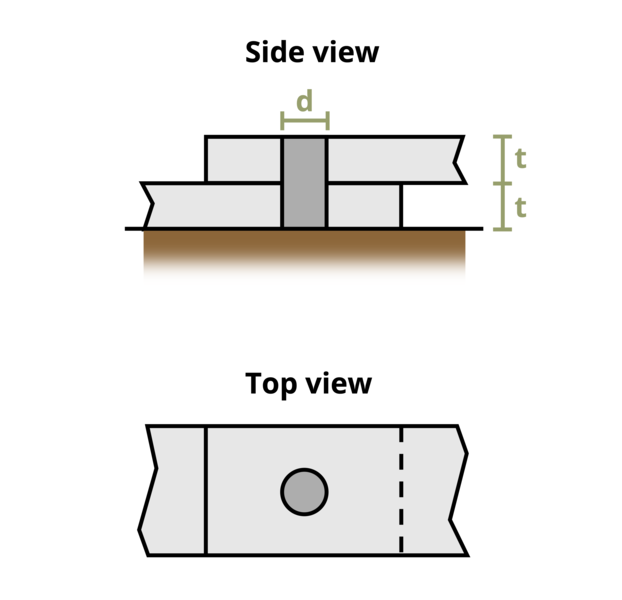
\includegraphics[keepaspectratio]{images/239.png}}
{[}Problem adapted from © Kurt Gramoll CC BY NC-SA 4.0{]}

\begin{Shaded}
\begin{Highlighting}[]
\NormalTok{\#| standalone: true}
\NormalTok{\#| viewerHeight: 600}
\NormalTok{\#| components: [viewer]}

\NormalTok{from shiny import App, render, ui, reactive}
\NormalTok{import random}
\NormalTok{import asyncio}
\NormalTok{import math}
\NormalTok{import io}
\NormalTok{import string}
\NormalTok{from datetime import datetime}
\NormalTok{from pathlib import Path}

\NormalTok{def generate\_random\_letters(length):}
\NormalTok{    \# Generate a random string of letters of specified length}
\NormalTok{    return \textquotesingle{}\textquotesingle{}.join(random.choice(string.ascii\_lowercase) for \_ in range(length))}

\NormalTok{problem\_ID="239"}
\NormalTok{t=reactive.Value("\_\_")}
\NormalTok{d=reactive.Value("\_\_")}
\NormalTok{delT=reactive.Value("\_\_")}
\NormalTok{Epin=reactive.Value("\_\_")}
\NormalTok{apin=reactive.Value("\_\_")}
\NormalTok{vpin=reactive.Value("\_\_")}

\NormalTok{attempts=["Timestamp,Attempt,Answer,Feedback\textbackslash{}n"]}

\NormalTok{app\_ui = ui.page\_fluid(}
\NormalTok{    \#ui.markdown("**Please enter your ID number from your instructor and click to generate your problem**"),}
\NormalTok{    \#ui.input\_text("ID","", placeholder="Enter ID Number Here"),}
\NormalTok{    \#ui.input\_action\_button("generate\_problem", "Generate Problem", class\_="btn{-}primary"),}
\NormalTok{    ui.markdown("**Problem Statement**"),}
\NormalTok{    ui.output\_ui("ui\_problem\_statement"),}
\NormalTok{    ui.input\_text("answer","Your Answer in units of in", placeholder="Please enter your answer"),}
\NormalTok{    ui.input\_action\_button("submit", "Check Answer", class\_="btn{-}primary"),}
\NormalTok{    \#ui.download\_button("download", "Download File to Submit", class\_="btn{-}success"),}
\NormalTok{)}

\NormalTok{def server(input, output, session):}
\NormalTok{    \# Initialize a counter for attempts}
\NormalTok{    attempt\_counter = reactive.Value(0)}

\NormalTok{    @output}
\NormalTok{    @render.ui}
\NormalTok{    def ui\_problem\_statement():}
\NormalTok{        randomize\_vars()}
\NormalTok{        return[ui.markdown(f"Two rigid plates of thickness t = \{t()\} in. are held together with a plastic pin of diameter d = \{d()\} in. If the temperature raises by ΔT = \{delT()\}°F, how far does the pin protrude from the top surface? Assume E\textless{}sub\textgreater{}pin\textless{}/sub\textgreater{} = \{Epin()\} ksi, α\textless{}sub\textgreater{}pin\textless{}/sub\textgreater{} = \{apin()\} x 10\textless{}sup\textgreater{}{-}6\textless{}/sup\textgreater{} /°F, and ν\textless{}sub\textgreater{}pin\textless{}/sub\textgreater{} = \{vpin()\}.")]}
    
\NormalTok{    \#@reactive.Effect}
\NormalTok{    \#@reactive.event(input.generate\_problem)}
\NormalTok{    def randomize\_vars():}
\NormalTok{        random.seed(101)}
\NormalTok{        t.set(random.randrange(30,80,1)/100)}
\NormalTok{        d.set(random.randrange(30,80,1)/100)}
\NormalTok{        delT.set(random.randrange(50,150,1))}
\NormalTok{        Epin.set(random.randrange(800,1200,10))}
\NormalTok{        apin.set(random.randrange(80,120,1)/10)}
\NormalTok{        vpin.set(random.randrange(35,45,1)/100)}
    
\NormalTok{    @reactive.Effect}
\NormalTok{    @reactive.event(input.submit)}
\NormalTok{    def \_():}
\NormalTok{        attempt\_counter.set(attempt\_counter() + 1)  \# Increment the attempt counter on each submission.}
\NormalTok{        dzT = apin()*10**{-}6*delT()*2*t()}
\NormalTok{        dxT = apin()*10**{-}6*delT()*d()}
\NormalTok{        exM = dxT/d()}
\NormalTok{        ezM = vpin()*2*exM/(1{-}vpin())}
\NormalTok{        dzM = ezM*2*t()}
\NormalTok{        instr = dzT+dzM}
\NormalTok{        if math.isclose(float(input.answer()), instr, rel\_tol=0.01):}
\NormalTok{            check = "*Correct*"}
\NormalTok{            correct\_indicator = "JL"}
\NormalTok{        else:}
\NormalTok{            check = "*Not Correct.*"}
\NormalTok{            correct\_indicator = "JG"}

\NormalTok{        \# Generate random parts for the encoded attempt.}
\NormalTok{        random\_start = generate\_random\_letters(4)}
\NormalTok{        random\_middle = generate\_random\_letters(4)}
\NormalTok{        random\_end = generate\_random\_letters(4)}
\NormalTok{        \#encoded\_attempt = f"\{random\_start\}\{problem\_ID\}{-}\{random\_middle\}\{attempt\_counter()\}\{correct\_indicator\}{-}\{random\_end\}\{input.ID()\}"}

\NormalTok{        \# Store the most recent encoded attempt in a reactive value so it persists across submissions}
\NormalTok{        \#session.encoded\_attempt = reactive.Value(encoded\_attempt)}

\NormalTok{        \# Append the attempt data to the attempts list without the encoded attempt}
\NormalTok{        attempts.append(f"\{datetime.now()\}, \{attempt\_counter()\}, \{input.answer()\}, \{check\}\textbackslash{}n")}

\NormalTok{        \# Show feedback to the user.}
\NormalTok{        feedback = ui.markdown(f"Your answer of \{input.answer()\} is \{check\}.")}
\NormalTok{        m = ui.modal(}
\NormalTok{            feedback,}
\NormalTok{            title="Feedback",}
\NormalTok{            easy\_close=True}
\NormalTok{        )}
\NormalTok{        ui.modal\_show(m)}

\NormalTok{    \#@render.download(filename=lambda: f"Problem\_Log{-}\{problem\_ID\}{-}\{input.ID()\}.csv")}
\NormalTok{    async def download():}
\NormalTok{        \# Start the CSV with the encoded attempt (without label)}
\NormalTok{        final\_encoded = session.encoded\_attempt() if session.encoded\_attempt is not None else "No attempts"}
\NormalTok{        yield f"\{final\_encoded\}\textbackslash{}n\textbackslash{}n"}
        
\NormalTok{        \# Write the header for the remaining CSV data once}
\NormalTok{        yield "Timestamp,Attempt,Answer,Feedback\textbackslash{}n"}
        
\NormalTok{        \# Write the attempts data, ensure that the header from the attempts list is not written again}
\NormalTok{        for attempt in attempts[1:]:  \# Skip the first element which is the header}
\NormalTok{            await asyncio.sleep(0.25)  \# This delay may not be necessary; adjust as needed}
\NormalTok{            yield attempt}

\NormalTok{\# App installation}
\NormalTok{app = App(app\_ui, server)}
\end{Highlighting}
\end{Shaded}

\chapter*{Problem 5.68 - Thermal
Deformation}\label{problem-5.68---thermal-deformation}
\addcontentsline{toc}{chapter}{Problem 5.68 - Thermal Deformation}

\markboth{Problem 5.68 - Thermal Deformation}{Problem 5.68 - Thermal
Deformation}

\pandocbounded{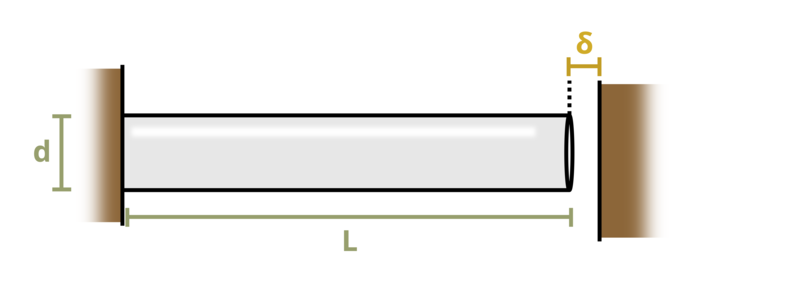
\includegraphics[keepaspectratio]{images/240.png}}
{[}Problem adapted from © Kurt Gramoll CC BY NC-SA 4.0{]}

\begin{Shaded}
\begin{Highlighting}[]
\NormalTok{\#| standalone: true}
\NormalTok{\#| viewerHeight: 600}
\NormalTok{\#| components: [viewer]}

\NormalTok{from shiny import App, render, ui, reactive}
\NormalTok{import random}
\NormalTok{import asyncio}
\NormalTok{import io}
\NormalTok{import math}
\NormalTok{import string}
\NormalTok{from datetime import datetime}
\NormalTok{from pathlib import Path}

\NormalTok{def generate\_random\_letters(length):}
\NormalTok{    \# Generate a random string of letters of specified length}
\NormalTok{    return \textquotesingle{}\textquotesingle{}.join(random.choice(string.ascii\_lowercase) for \_ in range(length))}

\NormalTok{problem\_ID="240"}
\NormalTok{L=reactive.Value("\_\_")}
\NormalTok{d=reactive.Value("\_\_")}
\NormalTok{delta=reactive.Value("\_\_")}
\NormalTok{delT = reactive.Value("\_\_")}
  
\NormalTok{attempts=["Timestamp,Attempt,Answer,Feedback\textbackslash{}n"]}

\NormalTok{app\_ui = ui.page\_fluid(}
\NormalTok{    \#ui.markdown("**Please enter your ID number from your instructor and click to generate your problem**"),}
\NormalTok{    \#ui.input\_text("ID","", placeholder="Enter ID Number Here"),}
\NormalTok{    \#ui.input\_action\_button("generate\_problem", "Generate Problem", class\_="btn{-}primary"),}
\NormalTok{    ui.markdown("**Problem Statement**"),}
\NormalTok{    ui.output\_ui("ui\_problem\_statement"),}
\NormalTok{    ui.input\_text("answer","Your Answer in units of mm", placeholder="Please enter your answer"),}
\NormalTok{    ui.input\_action\_button("submit", "Check Answer", class\_="btn{-}primary"),}
\NormalTok{    \#ui.download\_button("download", "Download File to Submit", class\_="btn{-}success"),}
\NormalTok{)}

\NormalTok{def server(input, output, session):}
\NormalTok{    \# Initialize a counter for attempts}
\NormalTok{    attempt\_counter = reactive.Value(0)}

\NormalTok{    @output}
\NormalTok{    @render.ui}
\NormalTok{    def ui\_problem\_statement():}
\NormalTok{        randomize\_vars()}
\NormalTok{        return[ui.markdown(f"A circular bar of length L = \{L()\} m and diameter d = \{d()\} mm is placed between two walls. The left end is fixed to the wall and the right end is ẟ = \{delta()\} mm from the wall. The temperature of the bar is raised ΔT = \{delT()\}°C. Determine the change in the bar\textquotesingle{}s diameter. Assume E = 3 GPa, α = 13.3 x 10\textless{}sup\textgreater{}{-}6\textless{}/sup\textgreater{} /°C, and ν = 0.32.")]}
    
\NormalTok{    \#@reactive.Effect}
\NormalTok{    \#@reactive.event(input.generate\_problem)}
\NormalTok{    def randomize\_vars():}
\NormalTok{        random.seed(101)}
\NormalTok{        L.set(random.randrange(30,80,1)/10)}
\NormalTok{        d.set(random.randrange(50,100,1))}
\NormalTok{        delta.set(random.randrange(5,50,1)/10)}
\NormalTok{        delT.set(random.randrange(150,350,1))}
        
\NormalTok{    @reactive.Effect}
\NormalTok{    @reactive.event(input.submit)}
\NormalTok{    def \_():}
\NormalTok{        attempt\_counter.set(attempt\_counter() + 1)  \# Increment the attempt counter on each submission.}
\NormalTok{        dTherm = 13.3*10**{-}6*delT()*L()}
\NormalTok{        sigmax = (delta()/1000{-}dTherm)/(L()/3000)}
\NormalTok{        ey = {-}0.32*sigmax/3000+13.3*10**{-}6*delT()}
\NormalTok{        instr = ey*d()}
\NormalTok{        if math.isclose(float(input.answer()), instr, rel\_tol=0.01):}
\NormalTok{            check = "*Correct*"}
\NormalTok{            correct\_indicator = "JL"}
\NormalTok{        else:}
\NormalTok{            check = "*Not Correct.*"}
\NormalTok{            correct\_indicator = "JG"}

\NormalTok{        \# Generate random parts for the encoded attempt.}
\NormalTok{        random\_start = generate\_random\_letters(4)}
\NormalTok{        random\_middle = generate\_random\_letters(4)}
\NormalTok{        random\_end = generate\_random\_letters(4)}
\NormalTok{        \#encoded\_attempt = f"\{random\_start\}\{problem\_ID\}{-}\{random\_middle\}\{attempt\_counter()\}\{correct\_indicator\}{-}\{random\_end\}\{input.ID()\}"}

\NormalTok{        \# Store the most recent encoded attempt in a reactive value so it persists across submissions}
\NormalTok{        \#session.encoded\_attempt = reactive.Value(encoded\_attempt)}

\NormalTok{        \# Append the attempt data to the attempts list without the encoded attempt}
\NormalTok{        attempts.append(f"\{datetime.now()\}, \{attempt\_counter()\}, \{input.answer()\}, \{check\}\textbackslash{}n")}

\NormalTok{        \# Show feedback to the user.}
\NormalTok{        feedback = ui.markdown(f"Your answer of \{input.answer()\} is \{check\}.")}
\NormalTok{        m = ui.modal(}
\NormalTok{            feedback,}
\NormalTok{            title="Feedback",}
\NormalTok{            easy\_close=True}
\NormalTok{        )}
\NormalTok{        ui.modal\_show(m)}

\NormalTok{    \#@render.download(filename=lambda: f"Problem\_Log{-}\{problem\_ID\}{-}\{input.ID()\}.csv")}
\NormalTok{    async def download():}
\NormalTok{        \# Start the CSV with the encoded attempt (without label)}
\NormalTok{        final\_encoded = session.encoded\_attempt() if session.encoded\_attempt is not None else "No attempts"}
\NormalTok{        yield f"\{final\_encoded\}\textbackslash{}n\textbackslash{}n"}
        
\NormalTok{        \# Write the header for the remaining CSV data once}
\NormalTok{        yield "Timestamp,Attempt,Answer,Feedback\textbackslash{}n"}
        
\NormalTok{        \# Write the attempts data, ensure that the header from the attempts list is not written again}
\NormalTok{        for attempt in attempts[1:]:  \# Skip the first element which is the header}
\NormalTok{            await asyncio.sleep(0.25)  \# This delay may not be necessary; adjust as needed}
\NormalTok{            yield attempt}

\NormalTok{\# App installation}
\NormalTok{app = App(app\_ui, server)}
\end{Highlighting}
\end{Shaded}

\chapter*{Problem 5.69 - Thermal
Deformation}\label{problem-5.69---thermal-deformation}
\addcontentsline{toc}{chapter}{Problem 5.69 - Thermal Deformation}

\markboth{Problem 5.69 - Thermal Deformation}{Problem 5.69 - Thermal
Deformation}

\pandocbounded{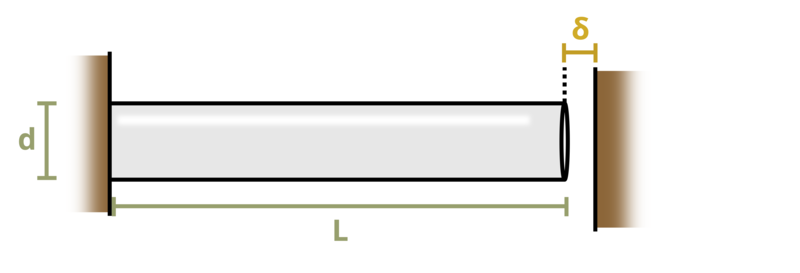
\includegraphics[keepaspectratio]{images/241.png}}
{[}Problem adapted from © Kurt Gramoll CC BY NC-SA 4.0{]}

\begin{Shaded}
\begin{Highlighting}[]
\NormalTok{\#| standalone: true}
\NormalTok{\#| viewerHeight: 600}
\NormalTok{\#| components: [viewer]}

\NormalTok{from shiny import App, render, ui, reactive}
\NormalTok{import random}
\NormalTok{import asyncio}
\NormalTok{import io}
\NormalTok{import math}
\NormalTok{import string}
\NormalTok{from datetime import datetime}
\NormalTok{from pathlib import Path}

\NormalTok{def generate\_random\_letters(length):}
\NormalTok{    \# Generate a random string of letters of specified length}
\NormalTok{    return \textquotesingle{}\textquotesingle{}.join(random.choice(string.ascii\_lowercase) for \_ in range(length))}

\NormalTok{problem\_ID="241"}
\NormalTok{L=reactive.Value("\_\_")}
\NormalTok{d=reactive.Value("\_\_")}
\NormalTok{delT = reactive.Value("\_\_")}

\NormalTok{attempts=["Timestamp,Attempt,Answer,Feedback\textbackslash{}n"]}

\NormalTok{app\_ui = ui.page\_fluid(}
\NormalTok{    \#ui.markdown("**Please enter your ID number from your instructor and click to generate your problem**"),}
\NormalTok{    \#ui.input\_text("ID","", placeholder="Enter ID Number Here"),}
\NormalTok{    \#ui.input\_action\_button("generate\_problem", "Generate Problem", class\_="btn{-}primary"),}
\NormalTok{    ui.markdown("**Problem Statement**"),}
\NormalTok{    ui.output\_ui("ui\_problem\_statement"),}
\NormalTok{    ui.input\_text("answer","Your Answer in units of ksi", placeholder="Please enter your answer"),}
\NormalTok{    ui.input\_action\_button("submit", "Check Answer", class\_="btn{-}primary"),}
\NormalTok{    \#ui.download\_button("download", "Download File to Submit", class\_="btn{-}success"),}
\NormalTok{)}

\NormalTok{def server(input, output, session):}
\NormalTok{    \# Initialize a counter for attempts}
\NormalTok{    attempt\_counter = reactive.Value(0)}

\NormalTok{    @output}
\NormalTok{    @render.ui}
\NormalTok{    def ui\_problem\_statement():}
\NormalTok{        randomize\_vars()}
\NormalTok{        return[ui.markdown(f"A circular bar of length L = \{L()\} in. and diameter d = \{d()\} in. is placed between two walls. The left end is fixed to the wall and the right end is ẟ =  0.01 in. from the wall. The temperature of the bar is raised ΔT = \{delT()\}°F. Determine the average normal stress in the bar. Assume E = 29,000 ksi and α = 7 x 10\textless{}sup\textgreater{}{-}6\textless{}/sup\textgreater{} /°F.")]}
    
\NormalTok{    \#@reactive.Effect}
\NormalTok{    \#@reactive.event(input.generate\_problem)}
\NormalTok{    def randomize\_vars():}
\NormalTok{        random.seed(101)}
\NormalTok{        L.set(random.randrange(10,30,1))}
\NormalTok{        d.set(random.randrange(3,20,1)/10)}
\NormalTok{        delT.set(random.randrange(150,350,1))}

\NormalTok{    @reactive.Effect}
\NormalTok{    @reactive.event(input.submit)}
\NormalTok{    def \_():}
\NormalTok{        attempt\_counter.set(attempt\_counter() + 1)  \# Increment the attempt counter on each submission.}
\NormalTok{        dTherm = 7*10**{-}6*delT()*L()}
\NormalTok{        instr = (dTherm{-}0.01/1000)/(L()/29000)}
\NormalTok{        if math.isclose(float(input.answer()), instr, rel\_tol=0.01):}
\NormalTok{            check = "*Correct*"}
\NormalTok{            correct\_indicator = "JL"}
\NormalTok{        else:}
\NormalTok{            check = "*Not Correct.*"}
\NormalTok{            correct\_indicator = "JG"}

\NormalTok{        \# Generate random parts for the encoded attempt.}
\NormalTok{        random\_start = generate\_random\_letters(4)}
\NormalTok{        random\_middle = generate\_random\_letters(4)}
\NormalTok{        random\_end = generate\_random\_letters(4)}
\NormalTok{        \#encoded\_attempt = f"\{random\_start\}\{problem\_ID\}{-}\{random\_middle\}\{attempt\_counter()\}\{correct\_indicator\}{-}\{random\_end\}\{input.ID()\}"}

\NormalTok{        \# Store the most recent encoded attempt in a reactive value so it persists across submissions}
\NormalTok{        \#session.encoded\_attempt = reactive.Value(encoded\_attempt)}

\NormalTok{        \# Append the attempt data to the attempts list without the encoded attempt}
\NormalTok{        attempts.append(f"\{datetime.now()\}, \{attempt\_counter()\}, \{input.answer()\}, \{check\}\textbackslash{}n")}

\NormalTok{        \# Show feedback to the user.}
\NormalTok{        feedback = ui.markdown(f"Your answer of \{input.answer()\} is \{check\}.")}
\NormalTok{        m = ui.modal(}
\NormalTok{            feedback,}
\NormalTok{            title="Feedback",}
\NormalTok{            easy\_close=True}
\NormalTok{        )}
\NormalTok{        ui.modal\_show(m)}

\NormalTok{    \#@render.download(filename=lambda: f"Problem\_Log{-}\{problem\_ID\}{-}\{input.ID()\}.csv")}
\NormalTok{    async def download():}
\NormalTok{        \# Start the CSV with the encoded attempt (without label)}
\NormalTok{        final\_encoded = session.encoded\_attempt() if session.encoded\_attempt is not None else "No attempts"}
\NormalTok{        yield f"\{final\_encoded\}\textbackslash{}n\textbackslash{}n"}
        
\NormalTok{        \# Write the header for the remaining CSV data once}
\NormalTok{        yield "Timestamp,Attempt,Answer,Feedback\textbackslash{}n"}
        
\NormalTok{        \# Write the attempts data, ensure that the header from the attempts list is not written again}
\NormalTok{        for attempt in attempts[1:]:  \# Skip the first element which is the header}
\NormalTok{            await asyncio.sleep(0.25)  \# This delay may not be necessary; adjust as needed}
\NormalTok{            yield attempt}

\NormalTok{\# App installation}
\NormalTok{app = App(app\_ui, server)}
\end{Highlighting}
\end{Shaded}

\chapter*{Problem 5.70 - Thermal
Deformation}\label{problem-5.70---thermal-deformation}
\addcontentsline{toc}{chapter}{Problem 5.70 - Thermal Deformation}

\markboth{Problem 5.70 - Thermal Deformation}{Problem 5.70 - Thermal
Deformation}

\pandocbounded{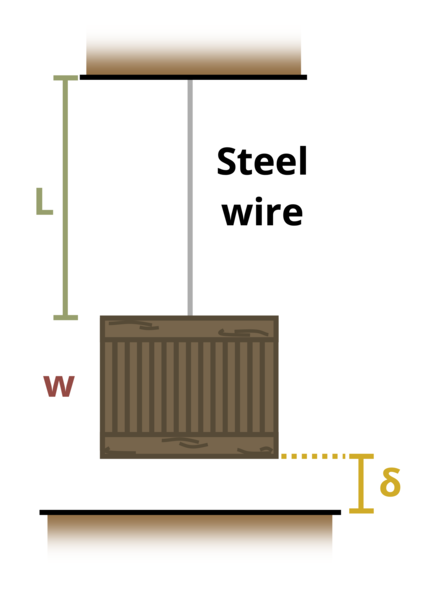
\includegraphics[keepaspectratio]{images/242.png}}
{[}Problem adapted from © Kurt Gramoll CC BY NC-SA 4.0{]}

\begin{Shaded}
\begin{Highlighting}[]
\NormalTok{\#| standalone: true}
\NormalTok{\#| viewerHeight: 600}
\NormalTok{\#| components: [viewer]}

\NormalTok{from shiny import App, render, ui, reactive}
\NormalTok{import random}
\NormalTok{import asyncio}
\NormalTok{import io}
\NormalTok{import math}
\NormalTok{import string}
\NormalTok{from datetime import datetime}
\NormalTok{from pathlib import Path}

\NormalTok{def generate\_random\_letters(length):}
\NormalTok{    \# Generate a random string of letters of specified length}
\NormalTok{    return \textquotesingle{}\textquotesingle{}.join(random.choice(string.ascii\_lowercase) for \_ in range(length))}

\NormalTok{problem\_ID="242"}
\NormalTok{W=reactive.Value("\_\_")}
\NormalTok{d=reactive.Value("\_\_")}
\NormalTok{L=reactive.Value("\_\_")}
\NormalTok{delta=reactive.Value("\_\_")}
\NormalTok{T1=reactive.Value("\_\_")}

\NormalTok{attempts=["Timestamp,Attempt,Answer,Feedback\textbackslash{}n"]}

\NormalTok{app\_ui = ui.page\_fluid(}
\NormalTok{    \#ui.markdown("**Please enter your ID number from your instructor and click to generate your problem**"),}
\NormalTok{    \#ui.input\_text("ID","", placeholder="Enter ID Number Here"),}
\NormalTok{    \#ui.input\_action\_button("generate\_problem", "Generate Problem", class\_="btn{-}primary"),}
\NormalTok{    ui.markdown("**Problem Statement**"),}
\NormalTok{    ui.output\_ui("ui\_problem\_statement"),}
\NormalTok{    ui.input\_text("answer","Your Answer in units of \textbackslash{}u00b0C", placeholder="Please enter your answer"),}
\NormalTok{    ui.input\_action\_button("submit", "Check Answer", class\_="btn{-}primary"),}
\NormalTok{    \#ui.download\_button("download", "Download File to Submit", class\_="btn{-}success"),}
\NormalTok{)}

\NormalTok{def server(input, output, session):}
\NormalTok{    \# Initialize a counter for attempts}
\NormalTok{    attempt\_counter = reactive.Value(0)}

\NormalTok{    @output}
\NormalTok{    @render.ui}
\NormalTok{    def ui\_problem\_statement():}
\NormalTok{        randomize\_vars()}
\NormalTok{        return[ui.markdown(f"A crate weighing W = \{W()\} kN is hung from a long steel cable of diameter d = \{d()\} mm and length L = \{L()\} m. The crate is initially ẟ = \{delta()\} mm above the ground when the temperature is T\textless{}sub\textgreater{}1\textless{}/sub\textgreater{} = \{T1()\}°C. At what temperature will the crate touch the ground. Assume E\textless{}sub\textgreater{}s\textless{}/sub\textgreater{} = 190 GPa and α\textless{}sub\textgreater{}s\textless{}/sub\textgreater{} = 6.5 x 10\textless{}sup\textgreater{}{-}6\textless{}/sup\textgreater{} /°C.")]}
    
\NormalTok{    \#@reactive.Effect}
\NormalTok{    \#@reactive.event(input.generate\_problem)}
\NormalTok{    def randomize\_vars():}
\NormalTok{        random.seed(101)}
\NormalTok{        W.set(random.randrange(50,100,1))}
\NormalTok{        d.set(random.randrange(50,100,1))}
\NormalTok{        L.set(random.randrange(50,100,1)/10)}
\NormalTok{        delta.set(random.randrange(5,10,1))}
\NormalTok{        T1.set(random.randrange(15,30,1))}
        
\NormalTok{    @reactive.Effect}
\NormalTok{    @reactive.event(input.submit)}
\NormalTok{    def \_():}
\NormalTok{        attempt\_counter.set(attempt\_counter() + 1)  \# Increment the attempt counter on each submission.}
\NormalTok{        dLoad = W()*1000*L()/((d()/1000/2)**2*math.pi*190*10**9)*1000}
\NormalTok{        instr = (delta(){-}dLoad+T1()*6.5*10**{-}6*L()*1000)/(6.5*10**{-}6*L()*1000)}
\NormalTok{        if math.isclose(float(input.answer()), instr, rel\_tol=0.01):}
\NormalTok{            check = "*Correct*"}
\NormalTok{            correct\_indicator = "JL"}
\NormalTok{        else:}
\NormalTok{            check = "*Not Correct*"}
\NormalTok{            correct\_indicator = "JG"}

\NormalTok{        \# Generate random parts for the encoded attempt.}
\NormalTok{        random\_start = generate\_random\_letters(4)}
\NormalTok{        random\_middle = generate\_random\_letters(4)}
\NormalTok{        random\_end = generate\_random\_letters(4)}
\NormalTok{        \#encoded\_attempt = f"\{random\_start\}\{problem\_ID\}{-}\{random\_middle\}\{attempt\_counter()\}\{correct\_indicator\}{-}\{random\_end\}\{input.ID()\}"}

\NormalTok{        \# Store the most recent encoded attempt in a reactive value so it persists across submissions}
\NormalTok{        \#session.encoded\_attempt = reactive.Value(encoded\_attempt)}

\NormalTok{        \# Append the attempt data to the attempts list without the encoded attempt}
\NormalTok{        attempts.append(f"\{datetime.now()\}, \{attempt\_counter()\}, \{input.answer()\}, \{check\}\textbackslash{}n")}

\NormalTok{        \# Show feedback to the user.}
\NormalTok{        feedback = ui.markdown(f"Your answer of \{input.answer()\} is \{check\}.")}
\NormalTok{        m = ui.modal(}
\NormalTok{            feedback,}
\NormalTok{            title="Feedback",}
\NormalTok{            easy\_close=True}
\NormalTok{        )}
\NormalTok{        ui.modal\_show(m)}

\NormalTok{    \#@render.download(filename=lambda: f"Problem\_Log{-}\{problem\_ID\}{-}\{input.ID()\}.csv")}
\NormalTok{    async def download():}
\NormalTok{        \# Start the CSV with the encoded attempt (without label)}
\NormalTok{        final\_encoded = session.encoded\_attempt() if session.encoded\_attempt is not None else "No attempts"}
\NormalTok{        yield f"\{final\_encoded\}\textbackslash{}n\textbackslash{}n"}
        
\NormalTok{        \# Write the header for the remaining CSV data once}
\NormalTok{        yield "Timestamp,Attempt,Answer,Feedback\textbackslash{}n"}
        
\NormalTok{        \# Write the attempts data, ensure that the header from the attempts list is not written again}
\NormalTok{        for attempt in attempts[1:]:  \# Skip the first element which is the header}
\NormalTok{            await asyncio.sleep(0.25)  \# This delay may not be necessary; adjust as needed}
\NormalTok{            yield attempt}

\NormalTok{\# App installation}
\NormalTok{app = App(app\_ui, server)}
\end{Highlighting}
\end{Shaded}

\chapter*{Problem 5.71 - Thermal
Deformation}\label{problem-5.71---thermal-deformation}
\addcontentsline{toc}{chapter}{Problem 5.71 - Thermal Deformation}

\markboth{Problem 5.71 - Thermal Deformation}{Problem 5.71 - Thermal
Deformation}

\pandocbounded{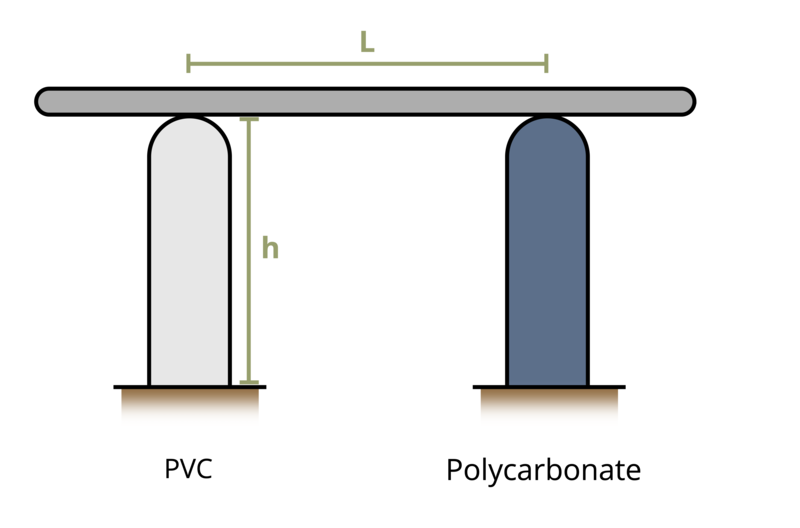
\includegraphics[keepaspectratio]{images/243.png}}
{[}Problem adapted from © Kurt Gramoll CC BY NC-SA 4.0{]}

\begin{Shaded}
\begin{Highlighting}[]
\NormalTok{\#| standalone: true}
\NormalTok{\#| viewerHeight: 600}
\NormalTok{\#| components: [viewer]}

\NormalTok{from shiny import App, render, ui, reactive}
\NormalTok{import random}
\NormalTok{import asyncio}
\NormalTok{import io}
\NormalTok{import math}
\NormalTok{import string}
\NormalTok{from datetime import datetime}
\NormalTok{from pathlib import Path}
\NormalTok{from math import atan, degrees}

\NormalTok{def generate\_random\_letters(length):}
\NormalTok{    \# Generate a random string of letters of specified length}
\NormalTok{    return \textquotesingle{}\textquotesingle{}.join(random.choice(string.ascii\_lowercase) for \_ in range(length))}

\NormalTok{problem\_ID="243"}
\NormalTok{L=reactive.Value("\_\_")}
\NormalTok{h=reactive.Value("\_\_")}
\NormalTok{delT=reactive.Value("\_\_")}
\NormalTok{apoly=reactive.Value("\_\_")}
\NormalTok{apvc=reactive.Value("\_\_")}

\NormalTok{attempts=["Timestamp,Attempt,Answer,Feedback\textbackslash{}n"]}

\NormalTok{app\_ui = ui.page\_fluid(}
\NormalTok{    \#ui.markdown("**Please enter your ID number from your instructor and click to generate your problem**"),}
\NormalTok{    \#ui.input\_text("ID","", placeholder="Enter ID Number Here"),}
\NormalTok{    \#ui.input\_action\_button("generate\_problem", "Generate Problem", class\_="btn{-}primary"),}
\NormalTok{    ui.markdown("**Problem Statement**"),}
\NormalTok{    ui.output\_ui("ui\_problem\_statement"),}
\NormalTok{    ui.input\_text("answer","Your Answer in units of °", placeholder="Please enter your answer"),}
\NormalTok{    ui.input\_action\_button("submit", "Check Answer", class\_="btn{-}primary"),}
\NormalTok{    \#ui.download\_button("download", "Download File to Submit", class\_="btn{-}success"),}
\NormalTok{)}

\NormalTok{def server(input, output, session):}
\NormalTok{    \# Initialize a counter for attempts}
\NormalTok{    attempt\_counter = reactive.Value(0)}

\NormalTok{    @output}
\NormalTok{    @render.ui}
\NormalTok{    def ui\_problem\_statement():}
\NormalTok{        randomize\_vars()}
\NormalTok{        return[ui.markdown(f"A rigid bar is supported by two posts made from PVC and polycarbonate, where length L = \{L()\} mm and height h = \{h()\} mm. The temperature of each post is raised by ΔT = \{delT()\}°C. Determine the angle of the bar with the ground. Assume α\textless{}sub\textgreater{}poly\textless{}/sub\textgreater{} = \{apoly()\} x 10\textless{}sup\textgreater{}{-}6\textless{}/sup\textgreater{} /°C and α\textless{}sub\textgreater{}PVC\textless{}/sub\textgreater{} = \{apvc()\} x 10\textless{}sup\textgreater{}{-}6\textless{}/sup\textgreater{} /°C.")]}
    
\NormalTok{    \#@reactive.Effect}
\NormalTok{    \#@reactive.event(input.generate\_problem)}
\NormalTok{    def randomize\_vars():}
\NormalTok{        random.seed(101)}
\NormalTok{        L.set(random.randrange(50,100,1))}
\NormalTok{        h.set(L()+random.randrange(15,40,1))}
\NormalTok{        delT.set(random.randrange(50,100,1))}
\NormalTok{        apoly.set(random.randrange(6,10,1)/10)}
\NormalTok{        apvc.set(random.randrange(40,60,1))}
        
\NormalTok{    @reactive.Effect}
\NormalTok{    @reactive.event(input.submit)}
\NormalTok{    def \_():}
\NormalTok{        attempt\_counter.set(attempt\_counter() + 1)  \# Increment the attempt counter on each submission.}
\NormalTok{        delpvc = apvc()*10**{-}6*delT()*L()}
\NormalTok{        delpoly = apoly()*10**{-}6*delT()*L()}
\NormalTok{        height = delpvc{-}delpoly}
\NormalTok{        instr = degrees(atan(height/L())) }
\NormalTok{        if math.isclose(float(input.answer()), instr, rel\_tol=0.01):}
\NormalTok{            check = "*Correct*"}
\NormalTok{            correct\_indicator = "JL"}
\NormalTok{        else:}
\NormalTok{            check = "*Not Correct*"}
\NormalTok{            correct\_indicator = "JG"}

\NormalTok{        \# Generate random parts for the encoded attempt.}
\NormalTok{        random\_start = generate\_random\_letters(4)}
\NormalTok{        random\_middle = generate\_random\_letters(4)}
\NormalTok{        random\_end = generate\_random\_letters(4)}
\NormalTok{        \#encoded\_attempt = f"\{random\_start\}\{problem\_ID\}{-}\{random\_middle\}\{attempt\_counter()\}\{correct\_indicator\}{-}\{random\_end\}\{input.ID()\}"}

\NormalTok{        \# Store the most recent encoded attempt in a reactive value so it persists across submissions}
\NormalTok{        \#session.encoded\_attempt = reactive.Value(encoded\_attempt)}

\NormalTok{        \# Append the attempt data to the attempts list without the encoded attempt}
\NormalTok{        attempts.append(f"\{datetime.now()\}, \{attempt\_counter()\}, \{input.answer()\}, \{check\}\textbackslash{}n")}

\NormalTok{        \# Show feedback to the user.}
\NormalTok{        feedback = ui.markdown(f"Your answer of \{input.answer()\} is \{check\}.")}
\NormalTok{        m = ui.modal(}
\NormalTok{            feedback,}
\NormalTok{            title="Feedback",}
\NormalTok{            easy\_close=True}
\NormalTok{        )}
\NormalTok{        ui.modal\_show(m)}

\NormalTok{    \#@render.download(filename=lambda: f"Problem\_Log{-}\{problem\_ID\}{-}\{input.ID()\}.csv")}
\NormalTok{    async def download():}
\NormalTok{        \# Start the CSV with the encoded attempt (without label)}
\NormalTok{        final\_encoded = session.encoded\_attempt() if session.encoded\_attempt is not None else "No attempts"}
\NormalTok{        yield f"\{final\_encoded\}\textbackslash{}n\textbackslash{}n"}
        
\NormalTok{        \# Write the header for the remaining CSV data once}
\NormalTok{        yield "Timestamp,Attempt,Answer,Feedback\textbackslash{}n"}
        
\NormalTok{        \# Write the attempts data, ensure that the header from the attempts list is not written again}
\NormalTok{        for attempt in attempts[1:]:  \# Skip the first element which is the header}
\NormalTok{            await asyncio.sleep(0.25)  \# This delay may not be necessary; adjust as needed}
\NormalTok{            yield attempt}

\NormalTok{\# App installation}
\NormalTok{app = App(app\_ui, server)}
\end{Highlighting}
\end{Shaded}

\chapter*{Problem 5.72 - Thermal
Deformation}\label{problem-5.72---thermal-deformation}
\addcontentsline{toc}{chapter}{Problem 5.72 - Thermal Deformation}

\markboth{Problem 5.72 - Thermal Deformation}{Problem 5.72 - Thermal
Deformation}

\pandocbounded{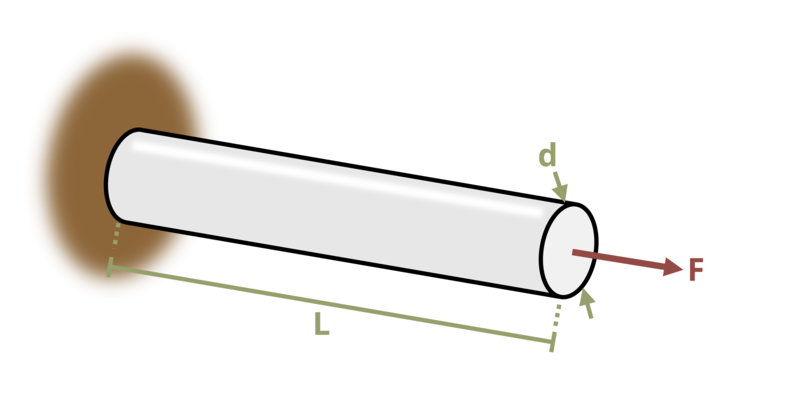
\includegraphics[keepaspectratio]{images/244.png}}
{[}Problem adapted from © Kurt Gramoll CC BY NC-SA 4.0{]}

\begin{Shaded}
\begin{Highlighting}[]
\NormalTok{\#| standalone: true}
\NormalTok{\#| viewerHeight: 600}
\NormalTok{\#| components: [viewer]}

\NormalTok{from shiny import App, render, ui, reactive}
\NormalTok{import random}
\NormalTok{import asyncio}
\NormalTok{import io}
\NormalTok{import math}
\NormalTok{import string}
\NormalTok{from datetime import datetime}
\NormalTok{from pathlib import Path}

\NormalTok{def generate\_random\_letters(length):}
\NormalTok{    \# Generate a random string of letters of specified length}
\NormalTok{    return \textquotesingle{}\textquotesingle{}.join(random.choice(string.ascii\_lowercase) for \_ in range(length))}

\NormalTok{problem\_ID="244"}
\NormalTok{L=reactive.Value("\_\_")}
\NormalTok{d=reactive.Value("\_\_")}
\NormalTok{delT=reactive.Value("\_\_")}

\NormalTok{attempts=["Timestamp,Attempt,Answer,Feedback\textbackslash{}n"]}

\NormalTok{app\_ui = ui.page\_fluid(}
\NormalTok{    \#ui.markdown("**Please enter your ID number from your instructor and click to generate your problem**"),}
\NormalTok{    \#ui.input\_text("ID","", placeholder="Enter ID Number Here"),}
\NormalTok{    \#ui.input\_action\_button("generate\_problem", "Generate Problem", class\_="btn{-}primary"),}
\NormalTok{    ui.markdown("**Problem Statement**"),}
\NormalTok{    ui.output\_ui("ui\_problem\_statement"),}
\NormalTok{    ui.input\_text("answer","Your Answer in units of kip", placeholder="Please enter your answer"),}
\NormalTok{    ui.input\_action\_button("submit", "Check Answer", class\_="btn{-}primary"),}
\NormalTok{    \#ui.download\_button("download", "Download File to Submit", class\_="btn{-}success"),}
\NormalTok{)}

\NormalTok{def server(input, output, session):}
\NormalTok{    \# Initialize a counter for attempts}
\NormalTok{    attempt\_counter = reactive.Value(0)}

\NormalTok{    @output}
\NormalTok{    @render.ui}
\NormalTok{    def ui\_problem\_statement():}
\NormalTok{        randomize\_vars()}
\NormalTok{        return[ui.markdown(f"A brass bar of length L = \{L()\} in. and diameter d = \{d()\} in. has its temperature increased by ΔT = \{delT()\}°F. Determine the force F required to keep the diameter of the bar constant. Assume E = 15,000 ksi, α = 11 x 10\textless{}sup\textgreater{}{-}6\textless{}/sup\textgreater{} /°F, and ν = 0.3.")]}
    
\NormalTok{    \#@reactive.Effect}
\NormalTok{    \#@reactive.event(input.generate\_problem)}
\NormalTok{    def randomize\_vars():}
\NormalTok{        random.seed(101)}
\NormalTok{        L.set(random.randrange(10,30,1))}
\NormalTok{        d.set(random.randrange(10,50,1)/10)}
\NormalTok{        delT.set(random.randrange(50,100,1))}
        
\NormalTok{    @reactive.Effect}
\NormalTok{    @reactive.event(input.submit)}
\NormalTok{    def \_():}
\NormalTok{        attempt\_counter.set(attempt\_counter() + 1)  \# Increment the attempt counter on each submission.}
\NormalTok{        dTherm = d()*11*10**{-}6*delT()}
\NormalTok{        dP = 0.3/((d()/2)**2*math.pi)/15000/d()}
\NormalTok{        instr = dTherm/dP}
\NormalTok{        if math.isclose(float(input.answer()), instr, rel\_tol=0.01):}
\NormalTok{            check = "*Correct*"}
\NormalTok{            correct\_indicator = "JL"}
\NormalTok{        else:}
\NormalTok{            check = "*Not Correct.*"}
\NormalTok{            correct\_indicator = "JG"}

\NormalTok{        \# Generate random parts for the encoded attempt.}
\NormalTok{        random\_start = generate\_random\_letters(4)}
\NormalTok{        random\_middle = generate\_random\_letters(4)}
\NormalTok{        random\_end = generate\_random\_letters(4)}
\NormalTok{        \#encoded\_attempt = f"\{random\_start\}\{problem\_ID\}{-}\{random\_middle\}\{attempt\_counter()\}\{correct\_indicator\}{-}\{random\_end\}\{input.ID()\}"}

\NormalTok{        \# Store the most recent encoded attempt in a reactive value so it persists across submissions}
\NormalTok{        \#session.encoded\_attempt = reactive.Value(encoded\_attempt)}

\NormalTok{        \# Append the attempt data to the attempts list without the encoded attempt}
\NormalTok{        attempts.append(f"\{datetime.now()\}, \{attempt\_counter()\}, \{input.answer()\}, \{check\}\textbackslash{}n")}

\NormalTok{        \# Show feedback to the user.}
\NormalTok{        feedback = ui.markdown(f"Your answer of \{input.answer()\} is \{check\}.")}
\NormalTok{        m = ui.modal(}
\NormalTok{            feedback,}
\NormalTok{            title="Feedback",}
\NormalTok{            easy\_close=True}
\NormalTok{        )}
\NormalTok{        ui.modal\_show(m)}

\NormalTok{    \#@render.download(filename=lambda: f"Problem\_Log{-}\{problem\_ID\}{-}\{input.ID()\}.csv")}
\NormalTok{    async def download():}
\NormalTok{        \# Start the CSV with the encoded attempt (without label)}
\NormalTok{        final\_encoded = session.encoded\_attempt() if session.encoded\_attempt is not None else "No attempts"}
\NormalTok{        yield f"\{final\_encoded\}\textbackslash{}n\textbackslash{}n"}
        
\NormalTok{        \# Write the header for the remaining CSV data once}
\NormalTok{        yield "Timestamp,Attempt,Answer,Feedback\textbackslash{}n"}
        
\NormalTok{        \# Write the attempts data, ensure that the header from the attempts list is not written again}
\NormalTok{        for attempt in attempts[1:]:  \# Skip the first element which is the header}
\NormalTok{            await asyncio.sleep(0.25)  \# This delay may not be necessary; adjust as needed}
\NormalTok{            yield attempt}

\NormalTok{\# App installation}
\NormalTok{app = App(app\_ui, server)}
\end{Highlighting}
\end{Shaded}

\chapter*{Problem 5.73 - Thermal
Deformation}\label{problem-5.73---thermal-deformation}
\addcontentsline{toc}{chapter}{Problem 5.73 - Thermal Deformation}

\markboth{Problem 5.73 - Thermal Deformation}{Problem 5.73 - Thermal
Deformation}

\pandocbounded{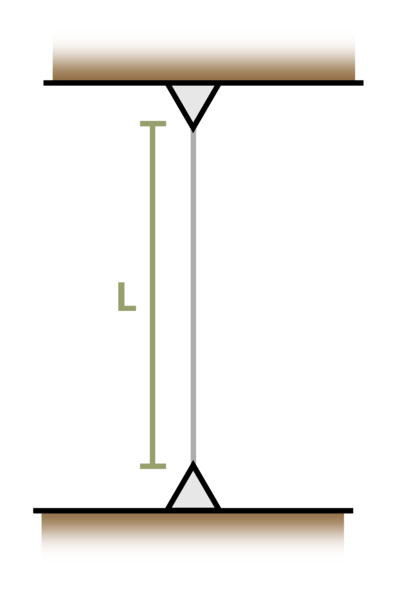
\includegraphics[keepaspectratio]{images/253.png}}
{[}Problem adapted from © Kurt Gramoll CC BY NC-SA 4.0{]}

\begin{Shaded}
\begin{Highlighting}[]
\NormalTok{\#| standalone: true}
\NormalTok{\#| viewerHeight: 600}
\NormalTok{\#| components: [viewer]}

\NormalTok{from shiny import App, render, ui, reactive}
\NormalTok{import random}
\NormalTok{import asyncio}
\NormalTok{import io}
\NormalTok{import math}
\NormalTok{import string}
\NormalTok{from datetime import datetime}
\NormalTok{from pathlib import Path}

\NormalTok{def generate\_random\_letters(length):}
\NormalTok{    \# Generate a random string of letters of specified length}
\NormalTok{    return \textquotesingle{}\textquotesingle{}.join(random.choice(string.ascii\_lowercase) for \_ in range(length))}

\NormalTok{problem\_ID="253"}
\NormalTok{L=reactive.Value("\_\_")}
\NormalTok{d=reactive.Value("\_\_")}
\NormalTok{delT=reactive.Value("\_\_")}
\NormalTok{E=reactive.Value("\_\_")}
\NormalTok{alpha=reactive.Value("\_\_")}

\NormalTok{attempts=["Timestamp,Attempt,Answer,Feedback\textbackslash{}n"]}

\NormalTok{app\_ui = ui.page\_fluid(}
\NormalTok{    \#ui.markdown("**Please enter your ID number from your instructor and click to generate your problem**"),}
\NormalTok{    \#ui.input\_text("ID","", placeholder="Enter ID Number Here"),}
\NormalTok{    \#ui.input\_action\_button("generate\_problem", "Generate Problem", class\_="btn{-}primary"),}
\NormalTok{    ui.markdown("**Problem Statement**"),}
\NormalTok{    ui.output\_ui("ui\_problem\_statement"),}
\NormalTok{    ui.input\_text("answer","Your Answer in units of MPa", placeholder="Please enter your answer"),}
\NormalTok{    ui.input\_action\_button("submit", "Check Answer", class\_="btn{-}primary"),}
\NormalTok{    \#ui.download\_button("download", "Download File to Submit", class\_="btn{-}success"),}
\NormalTok{)}

\NormalTok{def server(input, output, session):}
\NormalTok{    \# Initialize a counter for attempts}
\NormalTok{    attempt\_counter = reactive.Value(0)}

\NormalTok{    @output}
\NormalTok{    @render.ui}
\NormalTok{    def ui\_problem\_statement():}
\NormalTok{        randomize\_vars()}
\NormalTok{        return[ui.markdown(f"A cable of length L = \{L()\} m and diameter d = \{d()\} mm is connected between two fixed surfaces with no initial stress. The room is cooled by ΔT = \{delT()\}°C. Determine the stress in the cable. Assume E = \{E()\} GPa and α = \{alpha()\} x 10\textless{}sup\textgreater{}{-}6\textless{}/sup\textgreater{} /°C.")]}
    
\NormalTok{    \#@reactive.Effect}
\NormalTok{    \#@reactive.event(input.generate\_problem)}
\NormalTok{    def randomize\_vars():}
\NormalTok{        random.seed(101)}
\NormalTok{        L.set(random.randrange(20,100,1)/10)}
\NormalTok{        d.set(random.randrange(10,30,1))}
\NormalTok{        delT.set(random.randrange(50,150,1))}
\NormalTok{        E.set(random.randrange(175,225,1))}
\NormalTok{        alpha.set(random.randrange(80,130,1)/10)}
        
\NormalTok{    @reactive.Effect}
\NormalTok{    @reactive.event(input.submit)}
\NormalTok{    def \_():}
\NormalTok{        attempt\_counter.set(attempt\_counter() + 1)  \# Increment the attempt counter on each submission.}
\NormalTok{        instr = alpha()*10**{-}6*delT()*E()*10**3}
\NormalTok{        if math.isclose(float(input.answer()), instr, rel\_tol=0.01):}
\NormalTok{            check = "*Correct*"}
\NormalTok{            correct\_indicator = "JL"}
\NormalTok{        else:}
\NormalTok{            check = "*Not Correct.*"}
\NormalTok{            correct\_indicator = "JG"}

\NormalTok{        \# Generate random parts for the encoded attempt.}
\NormalTok{        random\_start = generate\_random\_letters(4)}
\NormalTok{        random\_middle = generate\_random\_letters(4)}
\NormalTok{        random\_end = generate\_random\_letters(4)}
\NormalTok{        \#encoded\_attempt = f"\{random\_start\}\{problem\_ID\}{-}\{random\_middle\}\{attempt\_counter()\}\{correct\_indicator\}{-}\{random\_end\}\{input.ID()\}"}

\NormalTok{        \# Store the most recent encoded attempt in a reactive value so it persists across submissions}
\NormalTok{        \#session.encoded\_attempt = reactive.Value(encoded\_attempt)}

\NormalTok{        \# Append the attempt data to the attempts list without the encoded attempt}
\NormalTok{        attempts.append(f"\{datetime.now()\}, \{attempt\_counter()\}, \{input.answer()\}, \{check\}\textbackslash{}n")}

\NormalTok{        \# Show feedback to the user.}
\NormalTok{        feedback = ui.markdown(f"Your answer of \{input.answer()\} is \{check\}.")}
\NormalTok{        m = ui.modal(}
\NormalTok{            feedback,}
\NormalTok{            title="Feedback",}
\NormalTok{            easy\_close=True}
\NormalTok{        )}
\NormalTok{        ui.modal\_show(m)}

\NormalTok{    \#@render.download(filename=lambda: f"Problem\_Log{-}\{problem\_ID\}{-}\{input.ID()\}.csv")}
\NormalTok{    async def download():}
\NormalTok{        \# Start the CSV with the encoded attempt (without label)}
\NormalTok{        final\_encoded = session.encoded\_attempt() if session.encoded\_attempt is not None else "No attempts"}
\NormalTok{        yield f"\{final\_encoded\}\textbackslash{}n\textbackslash{}n"}
        
\NormalTok{        \# Write the header for the remaining CSV data once}
\NormalTok{        yield "Timestamp,Attempt,Answer,Feedback\textbackslash{}n"}
        
\NormalTok{        \# Write the attempts data, ensure that the header from the attempts list is not written again}
\NormalTok{        for attempt in attempts[1:]:  \# Skip the first element which is the header}
\NormalTok{            await asyncio.sleep(0.25)  \# This delay may not be necessary; adjust as needed}
\NormalTok{            yield attempt}

\NormalTok{\# App installation}
\NormalTok{app = App(app\_ui, server)}
\end{Highlighting}
\end{Shaded}

\chapter*{Problem 5.74 - Thermal
Deformation}\label{problem-5.74---thermal-deformation}
\addcontentsline{toc}{chapter}{Problem 5.74 - Thermal Deformation}

\markboth{Problem 5.74 - Thermal Deformation}{Problem 5.74 - Thermal
Deformation}

\pandocbounded{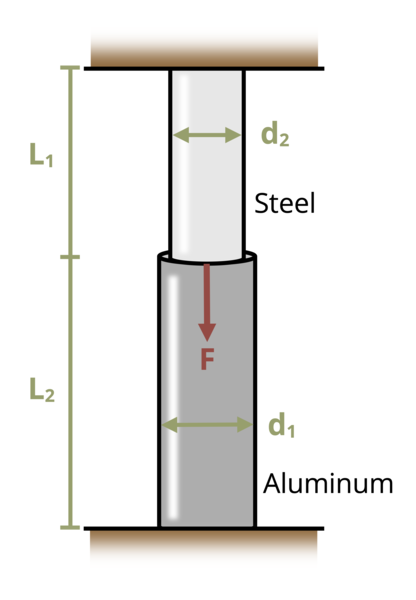
\includegraphics[keepaspectratio]{images/260.png}}
{[}Problem adapted from © Kurt Gramoll CC BY NC-SA 4.0{]}

\begin{Shaded}
\begin{Highlighting}[]
\NormalTok{\#| standalone: true}
\NormalTok{\#| viewerHeight: 600}
\NormalTok{\#| components: [viewer]}

\NormalTok{from shiny import App, render, ui, reactive}
\NormalTok{import random}
\NormalTok{import asyncio}
\NormalTok{import io}
\NormalTok{import math}
\NormalTok{import string}
\NormalTok{from datetime import datetime}
\NormalTok{from pathlib import Path}

\NormalTok{def generate\_random\_letters(length):}
\NormalTok{    \# Generate a random string of letters of specified length}
\NormalTok{    return \textquotesingle{}\textquotesingle{}.join(random.choice(string.ascii\_lowercase) for \_ in range(length))}

\NormalTok{problem\_ID="260"}
\NormalTok{delT=reactive.Value("\_\_")}
\NormalTok{F=reactive.Value("\_\_")}
\NormalTok{L1=reactive.Value("\_\_")}
\NormalTok{L2=reactive.Value("\_\_")}

\NormalTok{attempts=["Timestamp,Attempt,Answer,Feedback\textbackslash{}n"]}

\NormalTok{app\_ui = ui.page\_fluid(}
\NormalTok{    \#ui.markdown("**Please enter your ID number from your instructor and click to generate your problem**"),}
\NormalTok{    \#ui.input\_text("ID","", placeholder="Enter ID Number Here"),}
\NormalTok{    \#ui.input\_action\_button("generate\_problem", "Generate Problem", class\_="btn{-}primary"),}
\NormalTok{    ui.markdown("**Problem Statement**"),}
\NormalTok{    ui.output\_ui("ui\_problem\_statement"),}
\NormalTok{    ui.input\_text("answer","Your Answer in units of ksi", placeholder="Please enter your answer"),}
\NormalTok{    ui.input\_action\_button("submit", "Check Answer", class\_="btn{-}primary"),}
\NormalTok{    \#ui.download\_button("download", "Download File to Submit", class\_="btn{-}success"),}
\NormalTok{)}

\NormalTok{def server(input, output, session):}
\NormalTok{    \# Initialize a counter for attempts}
\NormalTok{    attempt\_counter = reactive.Value(0)}

\NormalTok{    @output}
\NormalTok{    @render.ui}
\NormalTok{    def ui\_problem\_statement():}
\NormalTok{        randomize\_vars()}
\NormalTok{        return[ui.markdown(f"Two circular rods are placed between two fixed walls as shown. The top rod is steel (E = 29,000 ksi, α = 6.5 x 10\textless{}sup\textgreater{}{-}6\textless{}/sup\textgreater{} /°F) and the bottom rod is aluminum (E = 10,000 ksi, α = 13 x 10\textless{}sub\textgreater{}{-}6\textless{}/sub\textgreater{} /°F). Determine the stress in the aluminum rod of the temperature increases by  ΔT  = \{delT()\}°F and a load F = \{F()\} kips is applied as shown. Assume L\textless{}sub\textgreater{}1\textless{}/sub\textgreater{} = \{L1()\} in., r\textless{}sub\textgreater{}1\textless{}/sub\textgreater{} = 1 in., L\textless{}sub\textgreater{}2\textless{}/sub\textgreater{} = \{L2()\} in., and r\textless{}sub\textgreater{}2\textless{}/sub\textgreater{} = 1.5 in.")]}
    
\NormalTok{    \#@reactive.Effect}
\NormalTok{    \#@reactive.event(input.generate\_problem)}
\NormalTok{    def randomize\_vars():}
\NormalTok{        random.seed(101)}
\NormalTok{        delT.set(random.randrange(100,200,1))}
\NormalTok{        F.set(random.randrange(10,50,1))}
\NormalTok{        L1.set(random.randrange(5,20,1))}
\NormalTok{        L2.set(L1()*1.3)}
    
\NormalTok{    @reactive.Effect}
\NormalTok{    @reactive.event(input.submit)}
\NormalTok{    def \_():}
\NormalTok{        attempt\_counter.set(attempt\_counter() + 1)  \# Increment the attempt counter on each submission.}
\NormalTok{        dTs = L1()*6.5*10**{-}6*delT()}
\NormalTok{        dTal = L2()*13*10**{-}6*delT()}
\NormalTok{        Fs = (dTs+dTal{-}(F()*1000*L2()/(10*10**6*0.75**2*math.pi)))/(L1()/(29*10**6*0.5**2*math.pi){-}L2()/(10*10**6*0.75**2*math.pi))}
\NormalTok{        Fal = Fs+F()*1000}
\NormalTok{        instr = Fal/(0.75**2*math.pi)/1000}
\NormalTok{        if math.isclose(float(input.answer()), instr, rel\_tol=0.01):}
\NormalTok{            check = "*Correct*"}
\NormalTok{            correct\_indicator = "JL"}
\NormalTok{        else:}
\NormalTok{            check = "*Not Correct.*"}
\NormalTok{            correct\_indicator = "JG"}

\NormalTok{        \# Generate random parts for the encoded attempt.}
\NormalTok{        random\_start = generate\_random\_letters(4)}
\NormalTok{        random\_middle = generate\_random\_letters(4)}
\NormalTok{        random\_end = generate\_random\_letters(4)}
\NormalTok{        \#encoded\_attempt = f"\{random\_start\}\{problem\_ID\}{-}\{random\_middle\}\{attempt\_counter()\}\{correct\_indicator\}{-}\{random\_end\}\{input.ID()\}"}

\NormalTok{        \# Store the most recent encoded attempt in a reactive value so it persists across submissions}
\NormalTok{        \#session.encoded\_attempt = reactive.Value(encoded\_attempt)}

\NormalTok{        \# Append the attempt data to the attempts list without the encoded attempt}
\NormalTok{        attempts.append(f"\{datetime.now()\}, \{attempt\_counter()\}, \{input.answer()\}, \{check\}\textbackslash{}n")}

\NormalTok{        \# Show feedback to the user.}
\NormalTok{        feedback = ui.markdown(f"Your answer of \{input.answer()\} is \{check\}.")}
\NormalTok{        m = ui.modal(}
\NormalTok{            feedback,}
\NormalTok{            title="Feedback",}
\NormalTok{            easy\_close=True}
\NormalTok{        )}
\NormalTok{        ui.modal\_show(m)}

\NormalTok{    \#@render.download(filename=lambda: f"Problem\_Log{-}\{problem\_ID\}{-}\{input.ID()\}.csv")}
\NormalTok{    async def download():}
\NormalTok{        \# Start the CSV with the encoded attempt (without label)}
\NormalTok{        final\_encoded = session.encoded\_attempt() if session.encoded\_attempt is not None else "No attempts"}
\NormalTok{        yield f"\{final\_encoded\}\textbackslash{}n\textbackslash{}n"}
        
\NormalTok{        \# Write the header for the remaining CSV data once}
\NormalTok{        yield "Timestamp,Attempt,Answer,Feedback\textbackslash{}n"}
        
\NormalTok{        \# Write the attempts data, ensure that the header from the attempts list is not written again}
\NormalTok{        for attempt in attempts[1:]:  \# Skip the first element which is the header}
\NormalTok{            await asyncio.sleep(0.25)  \# This delay may not be necessary; adjust as needed}
\NormalTok{            yield attempt}

\NormalTok{\# App installation}
\NormalTok{app = App(app\_ui, server)}
\end{Highlighting}
\end{Shaded}

\part{Chapter 6 Problems}

\chapter*{Problem 6.1 - Torsional
Stress}\label{problem-6.1---torsional-stress}
\addcontentsline{toc}{chapter}{Problem 6.1 - Torsional Stress}

\markboth{Problem 6.1 - Torsional Stress}{Problem 6.1 - Torsional
Stress}

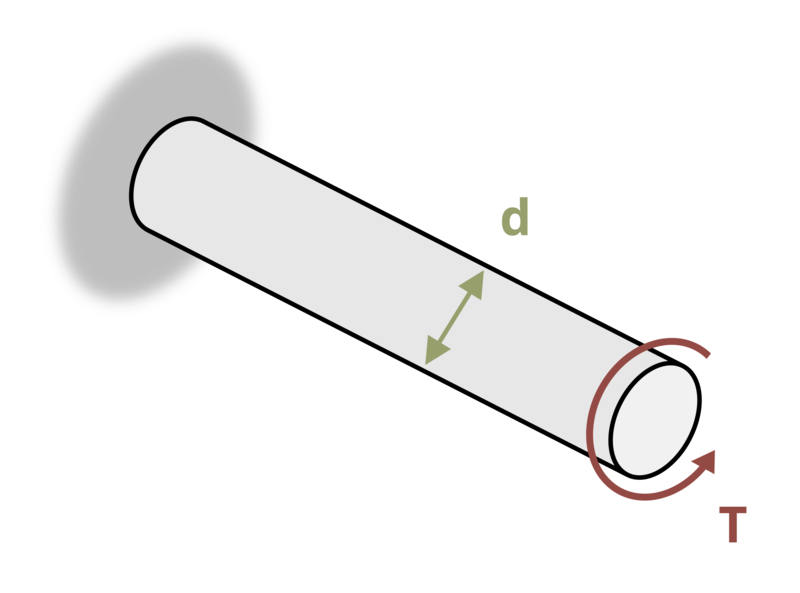
\includegraphics[width=2.60417in,height=\textheight,keepaspectratio]{images/265.png}
{[}Problem adapted from © Kurt Gramoll CC BY NC-SA 4.0{]}

\begin{Shaded}
\begin{Highlighting}[]
\NormalTok{\#| standalone: true}
\NormalTok{\#| viewerHeight: 600}
\NormalTok{\#| components: [viewer]}

\NormalTok{from shiny import App, render, ui, reactive}
\NormalTok{import random}
\NormalTok{import asyncio}
\NormalTok{import io}
\NormalTok{import math}
\NormalTok{import string}
\NormalTok{from datetime import datetime}
\NormalTok{from pathlib import Path}

\NormalTok{def generate\_random\_letters(length):}
\NormalTok{    \# Generate a random string of letters of specified length}
\NormalTok{    return \textquotesingle{}\textquotesingle{}.join(random.choice(string.ascii\_lowercase) for \_ in range(length)) }

\NormalTok{problem\_ID="265"}
\NormalTok{T=reactive.Value("\_\_")}
\NormalTok{d=reactive.Value("\_\_")}


\NormalTok{attempts=["Timestamp,Attempt,Answer,Feedback\textbackslash{}n"]}

\NormalTok{app\_ui = ui.page\_fluid(}
\NormalTok{    \#ui.markdown("**Please enter your ID number from your instructor and click to generate your problem**"),}
\NormalTok{    \#ui.input\_text("ID","", placeholder="Enter ID Number Here"),}
\NormalTok{    \#ui.input\_action\_button("generate\_problem", "Generate Problem", class\_="btn{-}primary"),}
\NormalTok{    ui.markdown("**Problem Statement**"),}
\NormalTok{    ui.output\_ui("ui\_problem\_statement"),}
\NormalTok{    ui.input\_text("answer","Your Answer in units of kN{-}m", placeholder="Please enter your answer"),}
\NormalTok{    ui.input\_action\_button("submit", "Check Answer", class\_="btn{-}primary"),}
\NormalTok{    \#ui.download\_button("download", "Download File to Submit", class\_="btn{-}success"),}
\NormalTok{)}


\NormalTok{def server(input, output, session):}
\NormalTok{    \# Initialize a counter for attempts}
\NormalTok{    attempt\_counter = reactive.Value(0)}

\NormalTok{    @output}
\NormalTok{    @render.ui}
\NormalTok{    def ui\_problem\_statement():}
\NormalTok{        randomize\_vars()}
\NormalTok{        return[ui.markdown(f"What torque is required to create a maximum shear stress of τ = \{T()\} MPa in a solid circular bar of diameter d  = \{d()\} mm? .")]}
    
\NormalTok{    \#@reactive.Effect}
\NormalTok{    \#@reactive.event(input.generate\_problem)}
\NormalTok{    def randomize\_vars():}
\NormalTok{        random.seed(101)}
\NormalTok{        T.set(random.randrange(20, 50, 1))}
\NormalTok{        d.set(random.randrange(50, 200, 1))}
        
\NormalTok{    @reactive.Effect}
\NormalTok{    @reactive.event(input.submit)}
\NormalTok{    def \_():}
\NormalTok{        attempt\_counter.set(attempt\_counter() + 1)  \# Increment the attempt counter on each submission.}
\NormalTok{        J = (math.pi/2)*(d()/2000)**4}
\NormalTok{        instr= (T()*1000*J)/(d()/2000)}
\NormalTok{        if math.isclose(float(input.answer()), instr, rel\_tol=0.01):}
\NormalTok{            check = "*Correct*"}
\NormalTok{            correct\_indicator = "JL"}
\NormalTok{        else:}
\NormalTok{            check = "*Not Correct.*"}
\NormalTok{            correct\_indicator = "JG"}

\NormalTok{        \# Generate random parts for the encoded attempt.}
\NormalTok{        random\_start = generate\_random\_letters(4)}
\NormalTok{        random\_middle = generate\_random\_letters(4)}
\NormalTok{        random\_end = generate\_random\_letters(4)}
\NormalTok{        \#encoded\_attempt = f"\{random\_start\}\{problem\_ID\}{-}\{random\_middle\}\{attempt\_counter()\}\{correct\_indicator\}{-}\{random\_end\}\{input.ID()\}"}

\NormalTok{        \# Store the most recent encoded attempt in a reactive value so it persists across submissions}
\NormalTok{        \#session.encoded\_attempt = reactive.Value(encoded\_attempt)}

\NormalTok{        \# Append the attempt data to the attempts list without the encoded attempt}
\NormalTok{        attempts.append(f"\{datetime.now()\}, \{attempt\_counter()\}, \{input.answer()\}, \{check\}\textbackslash{}n")}

\NormalTok{        \# Show feedback to the user.}
\NormalTok{        feedback = ui.markdown(f"Your answer of \{input.answer()\} is \{check\}.")}
\NormalTok{        m = ui.modal(}
\NormalTok{            feedback,}
\NormalTok{            title="Feedback",}
\NormalTok{            easy\_close=True}
\NormalTok{        )}
\NormalTok{        ui.modal\_show(m)}

\NormalTok{    \#@render.download(filename=lambda: f"Problem\_Log{-}\{problem\_ID\}{-}\{input.ID()\}.csv")}
\NormalTok{    async def download():}
\NormalTok{        \# Start the CSV with the encoded attempt (without label)}
\NormalTok{        final\_encoded = session.encoded\_attempt() if session.encoded\_attempt is not None else "No attempts"}
\NormalTok{        yield f"\{final\_encoded\}\textbackslash{}n\textbackslash{}n"}
        
\NormalTok{        \# Write the header for the remaining CSV data once}
\NormalTok{        yield "Timestamp,Attempt,Answer,Feedback\textbackslash{}n"}
        
\NormalTok{        \# Write the attempts data, ensure that the header from the attempts list is not written again}
\NormalTok{        for attempt in attempts[1:]:  \# Skip the first element which is the header}
\NormalTok{            await asyncio.sleep(0.25)  \# This delay may not be necessary; adjust as needed}
\NormalTok{            yield attempt}


\NormalTok{\# App installation}
\NormalTok{app = App(app\_ui, server)}
\end{Highlighting}
\end{Shaded}

\chapter*{Problem 6.2 - Torsional
Stress}\label{problem-6.2---torsional-stress}
\addcontentsline{toc}{chapter}{Problem 6.2 - Torsional Stress}

\markboth{Problem 6.2 - Torsional Stress}{Problem 6.2 - Torsional
Stress}

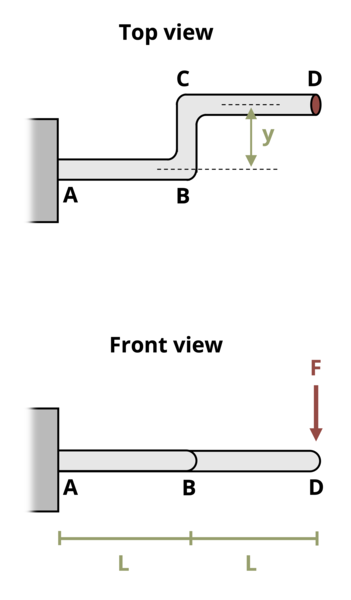
\includegraphics[width=3.125in,height=\textheight,keepaspectratio]{images/267.png}
{[}Problem adapted from © Kurt Gramoll CC BY NC-SA 4.0{]}

\begin{Shaded}
\begin{Highlighting}[]
\NormalTok{\#| standalone: true}
\NormalTok{\#| viewerHeight: 600}
\NormalTok{\#| components: [viewer]}

\NormalTok{from shiny import App, render, ui, reactive}
\NormalTok{import random}
\NormalTok{import asyncio}
\NormalTok{import io}
\NormalTok{import math}
\NormalTok{import string}
\NormalTok{from datetime import datetime}
\NormalTok{from pathlib import Path}

\NormalTok{def generate\_random\_letters(length):}
\NormalTok{    \# Generate a random string of letters of specified length}
\NormalTok{    return \textquotesingle{}\textquotesingle{}.join(random.choice(string.ascii\_lowercase) for \_ in range(length)) }

\NormalTok{problem\_ID="267"}
\NormalTok{F=reactive.Value("\_\_")}
\NormalTok{L=reactive.Value("\_\_")}
\NormalTok{y=reactive.Value("\_\_")}
\NormalTok{d=(reactive.Value("\_\_"))}

\NormalTok{attempts=["Timestamp,Attempt,Answer,Feedback\textbackslash{}n"]}

\NormalTok{app\_ui = ui.page\_fluid(}
\NormalTok{    \#ui.markdown("**Please enter your ID number from your instructor and click to generate your problem**"),}
\NormalTok{    \#ui.input\_text("ID","", placeholder="Enter ID Number Here"),}
\NormalTok{    \#ui.input\_action\_button("generate\_problem", "Generate Problem", class\_="btn{-}primary"),}
\NormalTok{    ui.markdown("**Problem Statement**"),}
\NormalTok{    ui.output\_ui("ui\_problem\_statement"),}
\NormalTok{    ui.input\_text("answer","Your Answer in units of ksi", placeholder="Please enter your answer"),}
\NormalTok{    ui.input\_action\_button("submit", "Check Answer", class\_="btn{-}primary"),}
\NormalTok{    \#ui.download\_button("download", "Download File to Submit", class\_="btn{-}success"),}
\NormalTok{)}


\NormalTok{def server(input, output, session):}
\NormalTok{    \# Initialize a counter for attempts}
\NormalTok{    attempt\_counter = reactive.Value(0)}

\NormalTok{    @output}
\NormalTok{    @render.ui}
\NormalTok{    def ui\_problem\_statement():}
\NormalTok{        randomize\_vars()}
\NormalTok{        return[ui.markdown(f"A force F = \{F()\} lb is applied to a hand crank that is stuck and will not turn. If L = \{L()\} in. and y = \{y()\} in., determine the maximum shear stress due to torsion in the crank rod between A and B. Assume the crank has diameter d = \{d()\} in.")]}
    
\NormalTok{    \#@reactive.Effect}
\NormalTok{    \#@reactive.event(input.generate\_problem)}
\NormalTok{    def randomize\_vars():}
\NormalTok{        random.seed(101)}
\NormalTok{        F.set(random.randrange(100, 350, 10))}
\NormalTok{        L.set(random.randrange(100, 200, 1)/10)}
\NormalTok{        y.set(round(L()/2, 2))}
\NormalTok{        d.set(random.randrange(3, 15, 1)/10)}
        
\NormalTok{    @reactive.Effect}
\NormalTok{    @reactive.event(input.submit)}
\NormalTok{    def \_():}
\NormalTok{        attempt\_counter.set(attempt\_counter() + 1)  \# Increment the attempt counter on each submission.}
\NormalTok{        T = F()*y()}
\NormalTok{        J = (math.pi/2)*(d()/2)**4}
\NormalTok{        instr= ((T*d()/2)/J)/10**3}
\NormalTok{        if math.isclose(float(input.answer()), instr, rel\_tol=0.01):}
\NormalTok{            check = "*Correct*"}
\NormalTok{            correct\_indicator = "JL"}
\NormalTok{        else:}
\NormalTok{            check = "*Not Correct.*"}
\NormalTok{            correct\_indicator = "JG"}

\NormalTok{        \# Generate random parts for the encoded attempt.}
\NormalTok{        random\_start = generate\_random\_letters(4)}
\NormalTok{        random\_middle = generate\_random\_letters(4)}
\NormalTok{        random\_end = generate\_random\_letters(4)}
\NormalTok{        \#encoded\_attempt = f"\{random\_start\}\{problem\_ID\}{-}\{random\_middle\}\{attempt\_counter()\}\{correct\_indicator\}{-}\{random\_end\}\{input.ID()\}"}

\NormalTok{        \# Store the most recent encoded attempt in a reactive value so it persists across submissions}
\NormalTok{        \#session.encoded\_attempt = reactive.Value(encoded\_attempt)}

\NormalTok{        \# Append the attempt data to the attempts list without the encoded attempt}
\NormalTok{        attempts.append(f"\{datetime.now()\}, \{attempt\_counter()\}, \{input.answer()\}, \{check\}\textbackslash{}n")}

\NormalTok{        \# Show feedback to the user.}
\NormalTok{        feedback = ui.markdown(f"Your answer of \{input.answer()\} is \{check\}.")}
\NormalTok{        m = ui.modal(}
\NormalTok{            feedback,}
\NormalTok{            title="Feedback",}
\NormalTok{            easy\_close=True}
\NormalTok{        )}
\NormalTok{        ui.modal\_show(m)}

\NormalTok{    \#@render.download(filename=lambda: f"Problem\_Log{-}\{problem\_ID\}{-}\{input.ID()\}.csv")}
\NormalTok{    async def download():}
\NormalTok{        \# Start the CSV with the encoded attempt (without label)}
\NormalTok{        final\_encoded = session.encoded\_attempt() if session.encoded\_attempt is not None else "No attempts"}
\NormalTok{        yield f"\{final\_encoded\}\textbackslash{}n\textbackslash{}n"}
        
\NormalTok{        \# Write the header for the remaining CSV data once}
\NormalTok{        yield "Timestamp,Attempt,Answer,Feedback\textbackslash{}n"}
        
\NormalTok{        \# Write the attempts data, ensure that the header from the attempts list is not written again}
\NormalTok{        for attempt in attempts[1:]:  \# Skip the first element which is the header}
\NormalTok{            await asyncio.sleep(0.25)  \# This delay may not be necessary; adjust as needed}
\NormalTok{            yield attempt}


\NormalTok{\# App installation}
\NormalTok{app = App(app\_ui, server)}
\end{Highlighting}
\end{Shaded}

\chapter*{Problem 6.3 - Torsional
Stress}\label{problem-6.3---torsional-stress}
\addcontentsline{toc}{chapter}{Problem 6.3 - Torsional Stress}

\markboth{Problem 6.3 - Torsional Stress}{Problem 6.3 - Torsional
Stress}

\pandocbounded{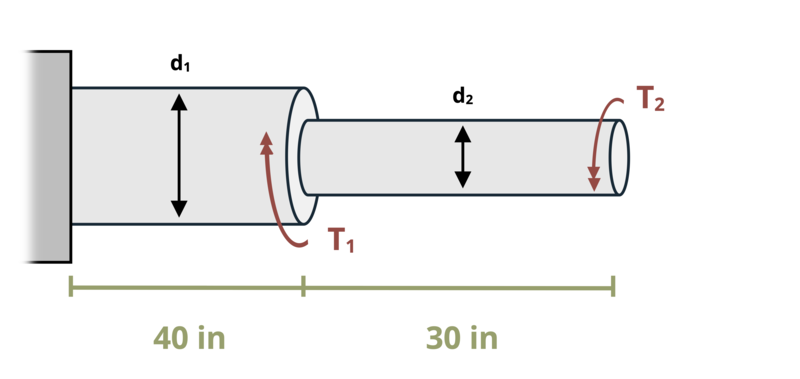
\includegraphics[keepaspectratio]{images/273.png}}
{[}Problem adapted from © Kurt Gramoll CC BY NC-SA 4.0{]}

\begin{Shaded}
\begin{Highlighting}[]
\NormalTok{\#| standalone: true}
\NormalTok{\#| viewerHeight: 600}
\NormalTok{\#| components: [viewer]}

\NormalTok{from shiny import App, render, ui, reactive}
\NormalTok{import random}
\NormalTok{import asyncio}
\NormalTok{import io}
\NormalTok{import math}
\NormalTok{import string}
\NormalTok{from datetime import datetime}
\NormalTok{from pathlib import Path}

\NormalTok{def generate\_random\_letters(length):}
\NormalTok{    \# Generate a random string of letters of specified length}
\NormalTok{    return \textquotesingle{}\textquotesingle{}.join(random.choice(string.ascii\_lowercase) for \_ in range(length)) }

\NormalTok{problem\_ID="273"}
\NormalTok{T1=reactive.Value("\_\_")}
\NormalTok{T2=reactive.Value("\_\_")}
\NormalTok{d1=reactive.Value("\_\_")}
\NormalTok{d2=reactive.Value("\_\_")}

\NormalTok{attempts=["Timestamp,Attempt,Answer,Feedback\textbackslash{}n"]}

\NormalTok{app\_ui = ui.page\_fluid(}
\NormalTok{    \#ui.markdown("**Please enter your ID number from your instructor and click to generate your problem**"),}
\NormalTok{    \#ui.input\_text("ID","", placeholder="Enter ID Number Here"),}
\NormalTok{    \#ui.input\_action\_button("generate\_problem", "Generate Problem", class\_="btn{-}primary"),}
\NormalTok{    ui.markdown("**Problem Statement**"),}
\NormalTok{    ui.output\_ui("ui\_problem\_statement"),}
\NormalTok{    ui.input\_text("answer","Your Answer in units of psi", placeholder="Please enter your answer"),}
\NormalTok{    ui.input\_action\_button("submit", "Check Answer", class\_="btn{-}primary"),}
\NormalTok{    \#ui.download\_button("download", "Download File to Submit", class\_="btn{-}success"),}
\NormalTok{)}

\NormalTok{def server(input, output, session):}
\NormalTok{    \# Initialize a counter for attempts}
\NormalTok{    attempt\_counter = reactive.Value(0)}

\NormalTok{    @output}
\NormalTok{    @render.ui}
\NormalTok{    def ui\_problem\_statement():}
\NormalTok{        randomize\_vars()}
\NormalTok{        return[ui.markdown(f"Two torques are applied to a two part circular rod as shown. If T\textless{}sub\textgreater{}1\textless{}/sub\textgreater{} = \{T1()\} kip{-}in., T\textless{}sub\textgreater{}2\textless{}/sub\textgreater{} = \{T2()\} kip{-}in., d\textless{}sub\textgreater{}1\textless{}/sub\textgreater{} = \{d1()\} in., and d\textless{}sub\textgreater{}2\textless{}/sub\textgreater{} = \{d2()\} in., what is the magnitude of the maximum shear stress?")]}
    
\NormalTok{    \#@reactive.Effect}
\NormalTok{    \#@reactive.event(input.generate\_problem)}
\NormalTok{    def randomize\_vars():}
\NormalTok{        random.seed(101)}
\NormalTok{        T1.set(random.randrange(5, 50, 1))}
\NormalTok{        T2.set(T1()*random.randrange(3, 5, 1)/10)}
\NormalTok{        d1.set(random.randrange(40, 80, 1)/10)}
\NormalTok{        d2.set(round(d1()*0.8, 2))}
        
\NormalTok{    @reactive.Effect}
\NormalTok{    @reactive.event(input.submit)}
\NormalTok{    def \_():}
\NormalTok{        attempt\_counter.set(attempt\_counter() + 1)  \# Increment the attempt counter on each submission.}
\NormalTok{        F1 = {-}T1()+T2()}
\NormalTok{        F2 = T2()}
\NormalTok{        J1 = (math.pi/2)*(d1()/2)**4}
\NormalTok{        J2 = (math.pi/2)*(d2()/2)**4}
\NormalTok{        tau1 = abs(F1*d1()/2/J1)*1000}
\NormalTok{        tau2 = abs(F2*d2()/2/J2)*1000}
\NormalTok{        if tau1\textgreater{}=tau2:}
\NormalTok{            instr = tau1}
\NormalTok{        else:}
\NormalTok{            instr = tau2}
\NormalTok{        if math.isclose(float(input.answer()), instr, rel\_tol=0.01):}
\NormalTok{            check = "*Correct*"}
\NormalTok{            correct\_indicator = "JL"}
\NormalTok{        else:}
\NormalTok{            check = "*Not Correct.*"}
\NormalTok{            correct\_indicator = "JG"}

\NormalTok{        \# Generate random parts for the encoded attempt.}
\NormalTok{        random\_start = generate\_random\_letters(4)}
\NormalTok{        random\_middle = generate\_random\_letters(4)}
\NormalTok{        random\_end = generate\_random\_letters(4)}
\NormalTok{        \#encoded\_attempt = f"\{random\_start\}\{problem\_ID\}{-}\{random\_middle\}\{attempt\_counter()\}\{correct\_indicator\}{-}\{random\_end\}\{input.ID()\}"}

\NormalTok{        \# Store the most recent encoded attempt in a reactive value so it persists across submissions}
\NormalTok{        \#session.encoded\_attempt = reactive.Value(encoded\_attempt)}

\NormalTok{        \# Append the attempt data to the attempts list without the encoded attempt}
\NormalTok{        attempts.append(f"\{datetime.now()\}, \{attempt\_counter()\}, \{input.answer()\}, \{check\}\textbackslash{}n")}

\NormalTok{        \# Show feedback to the user.}
\NormalTok{        feedback = ui.markdown(f"Your answer of \{input.answer()\} is \{check\}.")}
\NormalTok{        m = ui.modal(}
\NormalTok{            feedback,}
\NormalTok{            title="Feedback",}
\NormalTok{            easy\_close=True}
\NormalTok{        )}
\NormalTok{        ui.modal\_show(m)}

\NormalTok{    \#@render.download(filename=lambda: f"Problem\_Log{-}\{problem\_ID\}{-}\{input.ID()\}.csv")}
\NormalTok{    async def download():}
\NormalTok{        \# Start the CSV with the encoded attempt (without label)}
\NormalTok{        final\_encoded = session.encoded\_attempt() if session.encoded\_attempt is not None else "No attempts"}
\NormalTok{        yield f"\{final\_encoded\}\textbackslash{}n\textbackslash{}n"}
        
\NormalTok{        \# Write the header for the remaining CSV data once}
\NormalTok{        yield "Timestamp,Attempt,Answer,Feedback\textbackslash{}n"}
        
\NormalTok{        \# Write the attempts data, ensure that the header from the attempts list is not written again}
\NormalTok{        for attempt in attempts[1:]:  \# Skip the first element which is the header}
\NormalTok{            await asyncio.sleep(0.25)  \# This delay may not be necessary; adjust as needed}
\NormalTok{            yield attempt}

\NormalTok{\# App installation}
\NormalTok{app = App(app\_ui, server)}
\end{Highlighting}
\end{Shaded}

\chapter*{Problem 6.4 - Torsional
Stress}\label{problem-6.4---torsional-stress}
\addcontentsline{toc}{chapter}{Problem 6.4 - Torsional Stress}

\markboth{Problem 6.4 - Torsional Stress}{Problem 6.4 - Torsional
Stress}

\begin{figure}[H]

{\centering \pandocbounded{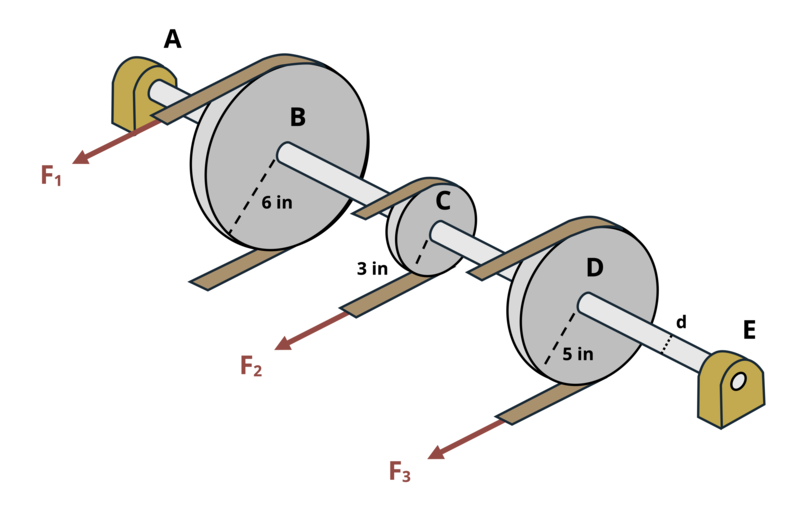
\includegraphics[keepaspectratio]{images/276.png}}

}

\caption{Figure 1: Three belt pullets are connected to a solid shaft.}

\end{figure}%

{[}Problem adapted from © Kurt Gramoll CC BY NC-SA 4.0{]}

\begin{Shaded}
\begin{Highlighting}[]
\NormalTok{\#| standalone: true}
\NormalTok{\#| viewerHeight: 600}
\NormalTok{\#| components: [viewer]}

\NormalTok{from shiny import App, render, ui, reactive}
\NormalTok{import random}
\NormalTok{import asyncio}
\NormalTok{import io}
\NormalTok{import math}
\NormalTok{import string}
\NormalTok{from datetime import datetime}
\NormalTok{from pathlib import Path}

\NormalTok{def generate\_random\_letters(length):}
\NormalTok{    \# Generate a random string of letters of specified length}
\NormalTok{    return \textquotesingle{}\textquotesingle{}.join(random.choice(string.ascii\_lowercase) for \_ in range(length)) }

\NormalTok{problem\_ID="276"}
\NormalTok{d=reactive.Value("\_\_")}
\NormalTok{F1=reactive.Value("\_\_")}
\NormalTok{F2=reactive.Value("\_\_")}
\NormalTok{F3=reactive.Value("\_\_")}

\NormalTok{attempts=["Timestamp,Attempt,Answer,Feedback\textbackslash{}n"]}

\NormalTok{app\_ui = ui.page\_fluid(}
\NormalTok{    \#ui.markdown("**Please enter your ID number from your instructor and click to generate your problem**"),}
\NormalTok{    \#ui.input\_text("ID","", placeholder="Enter ID Number Here"),}
\NormalTok{    \#ui.input\_action\_button("generate\_problem", "Generate Problem", class\_="btn{-}primary"),}
\NormalTok{    ui.markdown("**Problem Statement**"),}
\NormalTok{    ui.output\_ui("ui\_problem\_statement"),}
\NormalTok{    ui.input\_text("answer","Your Answer in units of ksi", placeholder="Please enter your answer"),}
\NormalTok{    ui.input\_action\_button("submit", "Check Answer", class\_="btn{-}primary"),}
\NormalTok{    \#ui.download\_button("download", "Download File to Submit", class\_="btn{-}success"),}
\NormalTok{)}


\NormalTok{def server(input, output, session):}
\NormalTok{    \# Initialize a counter for attempts}
\NormalTok{    attempt\_counter = reactive.Value(0)}

\NormalTok{    @output}
\NormalTok{    @render.ui}
\NormalTok{    def ui\_problem\_statement():}
\NormalTok{        randomize\_vars()}
\NormalTok{        return[ui.markdown(f"Three belt pulleys are connected to a solid circular shaft of diameter d = \{d()\} in. that rotates freely at joints A and E. The pulleys are subjected to forces F\textless{}sub\textgreater{}1\textless{}/sub\textgreater{} = \{F1()\} kips, F\textless{}sub\textgreater{}2\textless{}/sub\textgreater{} = \{F2()\} kips, and F\textless{}sub\textgreater{}3\textless{}/sub\textgreater{} = \{F3()\} kips. What is the maximum shear stress in the shaft between pulleys B and C?")]}
    
\NormalTok{    \#@reactive.Effect}
\NormalTok{    \#@reactive.event(input.generate\_problem)}
\NormalTok{    def randomize\_vars():}
\NormalTok{        random.seed(101)}
\NormalTok{        d.set(random.randrange(20, 40, 1)/10)}
\NormalTok{        F1.set(random.randrange(20, 200, 2)/10)}
\NormalTok{        F2.set(F1()/2)}
\NormalTok{        F3.set(round(F1()*0.9, 2))}
        
        
\NormalTok{    @reactive.Effect}
\NormalTok{    @reactive.event(input.submit)}
\NormalTok{    def \_():}
\NormalTok{        attempt\_counter.set(attempt\_counter() + 1)  \# Increment the attempt counter on each submission.}
\NormalTok{        T = 6*F1()}
\NormalTok{        instr= (T*(d()/2))/((math.pi/2)*(d()/2)**4)}
\NormalTok{        if math.isclose(float(input.answer()), instr, rel\_tol=0.01):}
\NormalTok{            check = "*Correct*"}
\NormalTok{            correct\_indicator = "JL"}
\NormalTok{        else:}
\NormalTok{            check = "*Not Correct.*"}
\NormalTok{            correct\_indicator = "JG"}

\NormalTok{        \# Generate random parts for the encoded attempt.}
\NormalTok{        random\_start = generate\_random\_letters(4)}
\NormalTok{        random\_middle = generate\_random\_letters(4)}
\NormalTok{        random\_end = generate\_random\_letters(4)}
\NormalTok{        \#encoded\_attempt = f"\{random\_start\}\{problem\_ID\}{-}\{random\_middle\}\{attempt\_counter()\}\{correct\_indicator\}{-}\{random\_end\}\{input.ID()\}"}

\NormalTok{        \# Store the most recent encoded attempt in a reactive value so it persists across submissions}
\NormalTok{        \#session.encoded\_attempt = reactive.Value(encoded\_attempt)}

\NormalTok{        \# Append the attempt data to the attempts list without the encoded attempt}
\NormalTok{        attempts.append(f"\{datetime.now()\}, \{attempt\_counter()\}, \{input.answer()\}, \{check\}\textbackslash{}n")}

\NormalTok{        \# Show feedback to the user.}
\NormalTok{        feedback = ui.markdown(f"Your answer of \{input.answer()\} is \{check\}.")}
\NormalTok{        m = ui.modal(}
\NormalTok{            feedback,}
\NormalTok{            title="Feedback",}
\NormalTok{            easy\_close=True}
\NormalTok{        )}
\NormalTok{        ui.modal\_show(m)}

\NormalTok{    \#@render.download(filename=lambda: f"Problem\_Log{-}\{problem\_ID\}{-}\{input.ID()\}.csv")}
\NormalTok{    async def download():}
\NormalTok{        \# Start the CSV with the encoded attempt (without label)}
\NormalTok{        final\_encoded = session.encoded\_attempt() if session.encoded\_attempt is not None else "No attempts"}
\NormalTok{        yield f"\{final\_encoded\}\textbackslash{}n\textbackslash{}n"}
        
\NormalTok{        \# Write the header for the remaining CSV data once}
\NormalTok{        yield "Timestamp,Attempt,Answer,Feedback\textbackslash{}n"}
        
\NormalTok{        \# Write the attempts data, ensure that the header from the attempts list is not written again}
\NormalTok{        for attempt in attempts[1:]:  \# Skip the first element which is the header}
\NormalTok{            await asyncio.sleep(0.25)  \# This delay may not be necessary; adjust as needed}
\NormalTok{            yield attempt}


\NormalTok{\# App installation}
\NormalTok{app = App(app\_ui, server)}
\end{Highlighting}
\end{Shaded}

\chapter*{Problem 6.5 - Torsional
Stress}\label{problem-6.5---torsional-stress}
\addcontentsline{toc}{chapter}{Problem 6.5 - Torsional Stress}

\markboth{Problem 6.5 - Torsional Stress}{Problem 6.5 - Torsional
Stress}

This is a dynamic rendering of the problem with dynamic variables based
on the username entered.

\pandocbounded{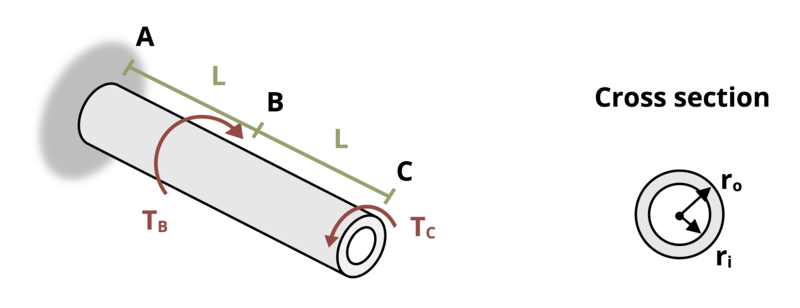
\includegraphics[keepaspectratio]{images/278.png}}
{[}Problem adapted from © Kurt Gramoll CC BY NC-SA 4.0{]}

\begin{Shaded}
\begin{Highlighting}[]
\NormalTok{\#| standalone: true}
\NormalTok{\#| viewerHeight: 600}
\NormalTok{\#| components: [viewer]}

\NormalTok{from shiny import App, render, ui, reactive}
\NormalTok{import random}
\NormalTok{import asyncio}
\NormalTok{import io}
\NormalTok{import math}
\NormalTok{import string}
\NormalTok{from datetime import datetime}
\NormalTok{from pathlib import Path}

\NormalTok{def generate\_random\_letters(length):}
\NormalTok{    \# Generate a random string of letters of specified length}
\NormalTok{    return \textquotesingle{}\textquotesingle{}.join(random.choice(string.ascii\_lowercase) for \_ in range(length)) }

\NormalTok{problem\_ID="278"}
\NormalTok{ro=reactive.Value("\_\_")}
\NormalTok{ri=reactive.Value("\_\_")}
\NormalTok{TB=reactive.Value("\_\_")}
\NormalTok{TC=reactive.Value("\_\_")}
\NormalTok{L=reactive.Value("\_\_")}

\NormalTok{attempts=["Timestamp,Attempt,Answer,Feedback\textbackslash{}n"]}

\NormalTok{app\_ui = ui.page\_fluid(}
\NormalTok{    \#ui.markdown("**Please enter your ID number from your instructor and click to generate your problem**"),}
\NormalTok{    \#ui.input\_text("ID","", placeholder="Enter ID Number Here"),}
\NormalTok{    \#ui.input\_action\_button("generate\_problem", "Generate Problem", class\_="btn{-}primary"),}
\NormalTok{    ui.markdown("**Problem Statement**"),}
\NormalTok{    ui.output\_ui("ui\_problem\_statement"),}
\NormalTok{    ui.input\_text("answer","Your Answer in units of ksi", placeholder="Please enter your answer"),}
\NormalTok{    ui.input\_action\_button("submit", "Check Answer", class\_="btn{-}primary"),}
\NormalTok{    \#ui.download\_button("download", "Download File to Submit", class\_="btn{-}success"),}
\NormalTok{)}


\NormalTok{def server(input, output, session):}
\NormalTok{    \# Initialize a counter for attempts}
\NormalTok{    attempt\_counter = reactive.Value(0)}

\NormalTok{    @output}
\NormalTok{    @render.ui}
\NormalTok{    def ui\_problem\_statement():}
\NormalTok{        randomize\_vars()}
\NormalTok{        return[ui.markdown(f"Two torques ,T\textless{}sub\textgreater{}B\textless{}/sub\textgreater{} = \{TB()\} kip{-}ft and T\textless{}sub\textgreater{}C\textless{}/sub\textgreater{} = \{TC()\} kip{-}ft, are applied to the hollow pipe as shown. If L = \{L()\} ft., r\textless{}sub\textgreater{}o\textless{}/sub\textgreater{} = \{ro()\} in., and r\textless{}sub\textgreater{}i\textless{}/sub\textgreater{} = \{ri()\} in., determine the maximum shear stress in the pipe.")]}
    
\NormalTok{    \#@reactive.Effect}
\NormalTok{    \#@reactive.event(input.generate\_problem)}
\NormalTok{    def randomize\_vars():}
\NormalTok{        random.seed(101)}
\NormalTok{        TB.set(random.randrange(100, 500, 100))}
\NormalTok{        TC.set(TB()/2)}
\NormalTok{        L.set(random.randrange(10, 90, 1)/10)}
\NormalTok{        ro.set(random.randrange(15, 60, 1)/10)}
\NormalTok{        ri.set(round(ro()*0.8,1))}
        
        
\NormalTok{    @reactive.Effect}
\NormalTok{    @reactive.event(input.submit)}
\NormalTok{    def \_():}
\NormalTok{        attempt\_counter.set(attempt\_counter() + 1)  \# Increment the attempt counter on each submission.}
\NormalTok{        Tmax = (TB(){-}TC())*12}
\NormalTok{        J = (math.pi/2)*(ro()**4 {-} ri()**4)}
\NormalTok{        instr= (Tmax*ro())/J}
\NormalTok{        if math.isclose(float(input.answer()), instr, rel\_tol=0.01):}
\NormalTok{            check = "*Correct*"}
\NormalTok{            correct\_indicator = "JL"}
\NormalTok{        else:}
\NormalTok{            check = "*Not Correct.*"}
\NormalTok{            correct\_indicator = "JG"}

\NormalTok{        \# Generate random parts for the encoded attempt.}
\NormalTok{        random\_start = generate\_random\_letters(4)}
\NormalTok{        random\_middle = generate\_random\_letters(4)}
\NormalTok{        random\_end = generate\_random\_letters(4)}
\NormalTok{        \#encoded\_attempt = f"\{random\_start\}\{problem\_ID\}{-}\{random\_middle\}\{attempt\_counter()\}\{correct\_indicator\}{-}\{random\_end\}\{input.ID()\}"}

\NormalTok{        \# Store the most recent encoded attempt in a reactive value so it persists across submissions}
\NormalTok{        \#session.encoded\_attempt = reactive.Value(encoded\_attempt)}

\NormalTok{        \# Append the attempt data to the attempts list without the encoded attempt}
\NormalTok{        attempts.append(f"\{datetime.now()\}, \{attempt\_counter()\}, \{input.answer()\}, \{check\}\textbackslash{}n")}

\NormalTok{        \# Show feedback to the user.}
\NormalTok{        feedback = ui.markdown(f"Your answer of \{input.answer()\} is \{check\}.")}
\NormalTok{        m = ui.modal(}
\NormalTok{            feedback,}
\NormalTok{            title="Feedback",}
\NormalTok{            easy\_close=True}
\NormalTok{        )}
\NormalTok{        ui.modal\_show(m)}

\NormalTok{    \#@render.download(filename=lambda: f"Problem\_Log{-}\{problem\_ID\}{-}\{input.ID()\}.csv")}
\NormalTok{    async def download():}
\NormalTok{        \# Start the CSV with the encoded attempt (without label)}
\NormalTok{        final\_encoded = session.encoded\_attempt() if session.encoded\_attempt is not None else "No attempts"}
\NormalTok{        yield f"\{final\_encoded\}\textbackslash{}n\textbackslash{}n"}
        
\NormalTok{        \# Write the header for the remaining CSV data once}
\NormalTok{        yield "Timestamp,Attempt,Answer,Feedback\textbackslash{}n"}
        
\NormalTok{        \# Write the attempts data, ensure that the header from the attempts list is not written again}
\NormalTok{        for attempt in attempts[1:]:  \# Skip the first element which is the header}
\NormalTok{            await asyncio.sleep(0.25)  \# This delay may not be necessary; adjust as needed}
\NormalTok{            yield attempt}

\NormalTok{\# App installation}
\NormalTok{app = App(app\_ui, server)}
\end{Highlighting}
\end{Shaded}

\chapter*{Problem 6.6 - Torsional
Stress}\label{problem-6.6---torsional-stress}
\addcontentsline{toc}{chapter}{Problem 6.6 - Torsional Stress}

\markboth{Problem 6.6 - Torsional Stress}{Problem 6.6 - Torsional
Stress}

\pandocbounded{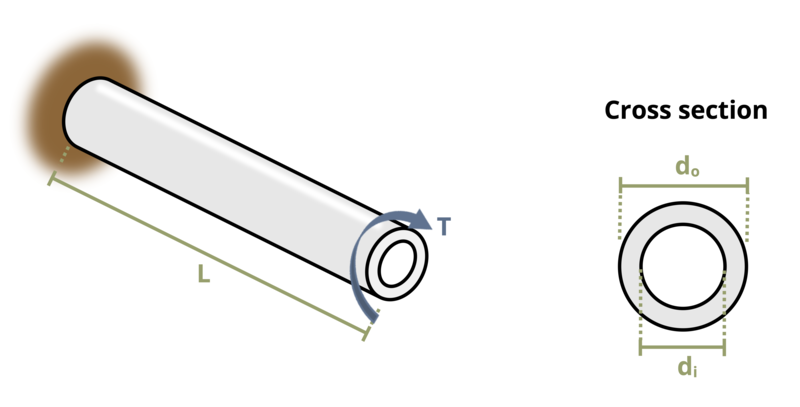
\includegraphics[keepaspectratio]{images/281.png}}
{[}Problem adapted from © Kurt Gramoll CC BY NC-SA 4.0{]}

\begin{Shaded}
\begin{Highlighting}[]
\NormalTok{\#| standalone: true}
\NormalTok{\#| viewerHeight: 600}
\NormalTok{\#| components: [viewer]}

\NormalTok{from shiny import App, render, ui, reactive}
\NormalTok{import random}
\NormalTok{import asyncio}
\NormalTok{import io}
\NormalTok{import math}
\NormalTok{import string}
\NormalTok{from datetime import datetime}
\NormalTok{from pathlib import Path}

\NormalTok{def generate\_random\_letters(length):}
\NormalTok{    \# Generate a random string of letters of specified length}
\NormalTok{    return \textquotesingle{}\textquotesingle{}.join(random.choice(string.ascii\_lowercase) for \_ in range(length))}

\NormalTok{problem\_ID="281"}
\NormalTok{do=reactive.Value("\_\_")}
\NormalTok{L=reactive.Value("\_\_")}
\NormalTok{T=reactive.Value("\_\_")}
\NormalTok{tmax=reactive.Value("\_\_")}

\NormalTok{attempts=["Timestamp,Attempt,Answer,Feedback\textbackslash{}n"]}

\NormalTok{app\_ui = ui.page\_fluid(}
\NormalTok{    \#ui.markdown("**Please enter your ID number from your instructor and click to generate your problem**"),}
\NormalTok{    \#ui.input\_text("ID","", placeholder="Enter ID Number Here"),}
\NormalTok{    \#ui.input\_action\_button("generate\_problem", "Generate Problem", class\_="btn{-}primary"),}
\NormalTok{    ui.markdown("**Problem Statement**"),}
\NormalTok{    ui.output\_ui("ui\_problem\_statement"),}
\NormalTok{    ui.input\_text("answer","Your Answer in units of in", placeholder="Please enter your answer"),}
\NormalTok{    ui.input\_action\_button("submit", "Check Answer", class\_="btn{-}primary"),}
\NormalTok{    \#ui.download\_button("download", "Download File to Submit", class\_="btn{-}success"),}
\NormalTok{)}

\NormalTok{def server(input, output, session):}
\NormalTok{    \# Initialize a counter for attempts}
\NormalTok{    attempt\_counter = reactive.Value(0)}

\NormalTok{    @output}
\NormalTok{    @render.ui}
\NormalTok{    def ui\_problem\_statement():}
\NormalTok{        randomize\_vars()}
\NormalTok{        return[ui.markdown(f"A hollow steel pole has an outer diameter d\textless{}sub\textgreater{}o\textless{}/sub\textgreater{} = \{do()\} in. and length L = \{L()\} ft. If the pole is subjected to torque T = \{T()\} lb{-}ft at its free end and the maximum shear stress, τ\textless{}sub\textgreater{}max\textless{}/sub\textgreater{}, is not to exceed \{tmax()\} psi, determine the maximum allowable inner diameter of the pole, d\textless{}sub\textgreater{}i\textless{}/sub\textgreater{}.")]}
    
\NormalTok{    \#@reactive.Effect}
\NormalTok{    \#@reactive.event(input.generate\_problem)}
\NormalTok{    def randomize\_vars():}
\NormalTok{        random.seed(101)}
\NormalTok{        do.set(random.randrange(40,100,1)/10)}
\NormalTok{        L.set(random.randrange(15,50,1)/10)}
\NormalTok{        T.set(random.randrange(350,750,10))}
\NormalTok{        tmax.set(random.randrange(250,400,10))}
        
\NormalTok{    @reactive.Effect}
\NormalTok{    @reactive.event(input.submit)}
\NormalTok{    def \_():}
\NormalTok{        attempt\_counter.set(attempt\_counter() + 1)  \# Increment the attempt counter on each submission.}
\NormalTok{        r1 = ((do()/2)**4{-}2*T()*do()/2/(math.pi*tmax()))**0.25}
\NormalTok{        instr = 2*r1}
\NormalTok{        if math.isclose(float(input.answer()), instr, rel\_tol=0.01):}
\NormalTok{            check = "*Correct*"}
\NormalTok{            correct\_indicator = "JL"}
\NormalTok{        else:}
\NormalTok{            check = "*Not Correct.*"}
\NormalTok{            correct\_indicator = "JG"}

\NormalTok{        \# Generate random parts for the encoded attempt.}
\NormalTok{        random\_start = generate\_random\_letters(4)}
\NormalTok{        random\_middle = generate\_random\_letters(4)}
\NormalTok{        random\_end = generate\_random\_letters(4)}
\NormalTok{        \#encoded\_attempt = f"\{random\_start\}\{problem\_ID\}{-}\{random\_middle\}\{attempt\_counter()\}\{correct\_indicator\}{-}\{random\_end\}\{input.ID()\}"}

\NormalTok{        \# Store the most recent encoded attempt in a reactive value so it persists across submissions}
\NormalTok{        \#session.encoded\_attempt = reactive.Value(encoded\_attempt)}

\NormalTok{        \# Append the attempt data to the attempts list without the encoded attempt}
\NormalTok{        attempts.append(f"\{datetime.now()\}, \{attempt\_counter()\}, \{input.answer()\}, \{check\}\textbackslash{}n")}

\NormalTok{        \# Show feedback to the user.}
\NormalTok{        feedback = ui.markdown(f"Your answer of \{input.answer()\} is \{check\}.")}
\NormalTok{        m = ui.modal(}
\NormalTok{            feedback,}
\NormalTok{            title="Feedback",}
\NormalTok{            easy\_close=True}
\NormalTok{        )}
\NormalTok{        ui.modal\_show(m)}

\NormalTok{    \#@render.download(filename=lambda: f"Problem\_Log{-}\{problem\_ID\}{-}\{input.ID()\}.csv")}
\NormalTok{    async def download():}
\NormalTok{        \# Start the CSV with the encoded attempt (without label)}
\NormalTok{        final\_encoded = session.encoded\_attempt() if session.encoded\_attempt is not None else "No attempts"}
\NormalTok{        yield f"\{final\_encoded\}\textbackslash{}n\textbackslash{}n"}
        
\NormalTok{        \# Write the header for the remaining CSV data once}
\NormalTok{        yield "Timestamp,Attempt,Answer,Feedback\textbackslash{}n"}
        
\NormalTok{        \# Write the attempts data, ensure that the header from the attempts list is not written again}
\NormalTok{        for attempt in attempts[1:]:  \# Skip the first element which is the header}
\NormalTok{            await asyncio.sleep(0.25)  \# This delay may not be necessary; adjust as needed}
\NormalTok{            yield attempt}

\NormalTok{\# App installation}
\NormalTok{app = App(app\_ui, server)}
\end{Highlighting}
\end{Shaded}

\chapter*{Problem 6.7 - Torsional
Stress}\label{problem-6.7---torsional-stress}
\addcontentsline{toc}{chapter}{Problem 6.7 - Torsional Stress}

\markboth{Problem 6.7 - Torsional Stress}{Problem 6.7 - Torsional
Stress}

\pandocbounded{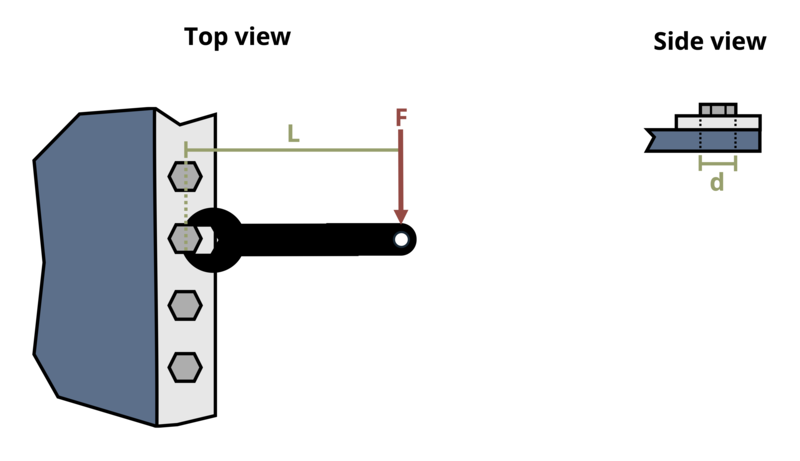
\includegraphics[keepaspectratio]{images/282.png}}
{[}Problem adapted from © Kurt Gramoll CC BY NC-SA 4.0{]}

\begin{Shaded}
\begin{Highlighting}[]
\NormalTok{\#| standalone: true}
\NormalTok{\#| viewerHeight: 600}
\NormalTok{\#| components: [viewer]}

\NormalTok{from shiny import App, render, ui, reactive}
\NormalTok{import random}
\NormalTok{import asyncio}
\NormalTok{import io}
\NormalTok{import math}
\NormalTok{import string}
\NormalTok{from datetime import datetime}
\NormalTok{from pathlib import Path}

\NormalTok{def generate\_random\_letters(length):}
\NormalTok{    \# Generate a random string of letters of specified length}
\NormalTok{    return \textquotesingle{}\textquotesingle{}.join(random.choice(string.ascii\_lowercase) for \_ in range(length))}

\NormalTok{problem\_ID="282"}
\NormalTok{L=reactive.Value("\_\_")}
\NormalTok{F=reactive.Value("\_\_")}
\NormalTok{d=reactive.Value("\_\_")}

\NormalTok{attempts=["Timestamp,Attempt,Answer,Feedback\textbackslash{}n"]}

\NormalTok{app\_ui = ui.page\_fluid(}
\NormalTok{    \#ui.markdown("**Please enter your ID number from your instructor and click to generate your problem**"),}
\NormalTok{    \#ui.input\_text("ID","", placeholder="Enter ID Number Here"),}
\NormalTok{    \#ui.input\_action\_button("generate\_problem", "Generate Problem", class\_="btn{-}primary"),}
\NormalTok{    ui.markdown("**Problem Statement**"),}
\NormalTok{    ui.output\_ui("ui\_problem\_statement"),}
\NormalTok{    ui.input\_text("answer","Your Answer in units of MPa", placeholder="Please enter your answer"),}
\NormalTok{    ui.input\_action\_button("submit", "Check Answer", class\_="btn{-}primary"),}
\NormalTok{    \#ui.download\_button("download", "Download File to Submit", class\_="btn{-}success"),}
\NormalTok{)}

\NormalTok{def server(input, output, session):}
\NormalTok{    \# Initialize a counter for attempts}
\NormalTok{    attempt\_counter = reactive.Value(0)}

\NormalTok{    @output}
\NormalTok{    @render.ui}
\NormalTok{    def ui\_problem\_statement():}
\NormalTok{        randomize\_vars()}
\NormalTok{        return[ui.markdown(f"A bolt is tightened using a wrench of length L = \{L()\} mm and a force F = \{F()\} N. If the bolt has diameter d = \{d()\} mm and doesn\textquotesingle{}t rotate, determine the maximum shear stress in the bolt.")]}
    
\NormalTok{    \#@reactive.Effect}
\NormalTok{    \#@reactive.event(input.generate\_problem)}
\NormalTok{    def randomize\_vars():}
\NormalTok{        random.seed(101)}
\NormalTok{        L.set(random.randrange(250,500,10))}
\NormalTok{        F.set(random.randrange(75,200,1))}
\NormalTok{        d.set(random.randrange(10,30,1))}
        
\NormalTok{    @reactive.Effect}
\NormalTok{    @reactive.event(input.submit)}
\NormalTok{    def \_():}
\NormalTok{        attempt\_counter.set(attempt\_counter() + 1)  \# Increment the attempt counter on each submission.}
\NormalTok{        T = F()*L()/1000}
\NormalTok{        J = math.pi*(d()/2000)**4/2}
\NormalTok{        instr = T*d()/2000/J/1000000}
\NormalTok{        if math.isclose(float(input.answer()), instr, rel\_tol=0.01):}
\NormalTok{            check = "*Correct*"}
\NormalTok{            correct\_indicator = "JL"}
\NormalTok{        else:}
\NormalTok{            check = "*Not Correct.*"}
\NormalTok{            correct\_indicator = "JG"}

\NormalTok{        \# Generate random parts for the encoded attempt.}
\NormalTok{        random\_start = generate\_random\_letters(4)}
\NormalTok{        random\_middle = generate\_random\_letters(4)}
\NormalTok{        random\_end = generate\_random\_letters(4)}
\NormalTok{        \#encoded\_attempt = f"\{random\_start\}\{problem\_ID\}{-}\{random\_middle\}\{attempt\_counter()\}\{correct\_indicator\}{-}\{random\_end\}\{input.ID()\}"}

\NormalTok{        \# Store the most recent encoded attempt in a reactive value so it persists across submissions}
\NormalTok{        \#session.encoded\_attempt = reactive.Value(encoded\_attempt)}

\NormalTok{        \# Append the attempt data to the attempts list without the encoded attempt}
\NormalTok{        attempts.append(f"\{datetime.now()\}, \{attempt\_counter()\}, \{input.answer()\}, \{check\}\textbackslash{}n")}

\NormalTok{        \# Show feedback to the user.}
\NormalTok{        feedback = ui.markdown(f"Your answer of \{input.answer()\} is \{check\}.")}
\NormalTok{        m = ui.modal(}
\NormalTok{            feedback,}
\NormalTok{            title="Feedback",}
\NormalTok{            easy\_close=True}
\NormalTok{        )}
\NormalTok{        ui.modal\_show(m)}

\NormalTok{    \#@render.download(filename=lambda: f"Problem\_Log{-}\{problem\_ID\}{-}\{input.ID()\}.csv")}
\NormalTok{    async def download():}
\NormalTok{        \# Start the CSV with the encoded attempt (without label)}
\NormalTok{        final\_encoded = session.encoded\_attempt() if session.encoded\_attempt is not None else "No attempts"}
\NormalTok{        yield f"\{final\_encoded\}\textbackslash{}n\textbackslash{}n"}
        
\NormalTok{        \# Write the header for the remaining CSV data once}
\NormalTok{        yield "Timestamp,Attempt,Answer,Feedback\textbackslash{}n"}
        
\NormalTok{        \# Write the attempts data, ensure that the header from the attempts list is not written again}
\NormalTok{        for attempt in attempts[1:]:  \# Skip the first element which is the header}
\NormalTok{            await asyncio.sleep(0.25)  \# This delay may not be necessary; adjust as needed}
\NormalTok{            yield attempt}

\NormalTok{\# App installation}
\NormalTok{app = App(app\_ui, server)}
\end{Highlighting}
\end{Shaded}

\chapter*{Problem 6.8 - Torsional
Stress}\label{problem-6.8---torsional-stress}
\addcontentsline{toc}{chapter}{Problem 6.8 - Torsional Stress}

\markboth{Problem 6.8 - Torsional Stress}{Problem 6.8 - Torsional
Stress}

\pandocbounded{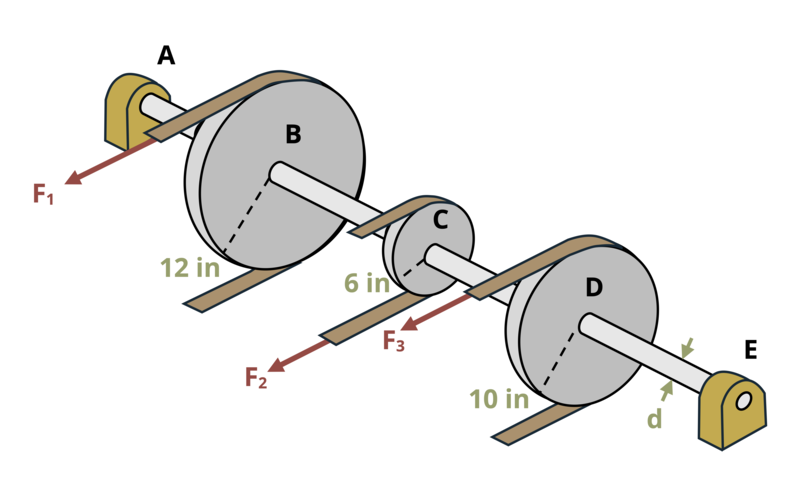
\includegraphics[keepaspectratio]{images/291.png}}
{[}Problem adapted from © Kurt Gramoll CC BY NC-SA 4.0{]}

\begin{Shaded}
\begin{Highlighting}[]
\NormalTok{\#| standalone: true}
\NormalTok{\#| viewerHeight: 600}
\NormalTok{\#| components: [viewer]}

\NormalTok{from shiny import App, render, ui, reactive}
\NormalTok{import random}
\NormalTok{import asyncio}
\NormalTok{import io}
\NormalTok{import math}
\NormalTok{import string}
\NormalTok{from datetime import datetime}
\NormalTok{from pathlib import Path}

\NormalTok{def generate\_random\_letters(length):}
\NormalTok{    \# Generate a random string of letters of specified length}
\NormalTok{    return \textquotesingle{}\textquotesingle{}.join(random.choice(string.ascii\_lowercase) for \_ in range(length))  }

\NormalTok{problem\_ID="291"}
\NormalTok{d=reactive.Value("\_\_")}
\NormalTok{F1=reactive.Value("\_\_")}
\NormalTok{F2=reactive.Value("\_\_")}
\NormalTok{F3=reactive.Value("\_\_")}
  
\NormalTok{attempts=["Timestamp,Attempt,Answer,Feedback\textbackslash{}n"]}

\NormalTok{app\_ui = ui.page\_fluid(}
\NormalTok{    \#ui.markdown("**Please enter your ID number from your instructor and click to generate your problem**"),}
\NormalTok{    \#ui.input\_text("ID","", placeholder="Enter ID Number Here"),}
\NormalTok{    \#ui.input\_action\_button("generate\_problem", "Generate Problem", class\_="btn{-}primary"),}
\NormalTok{    ui.markdown("**Problem Statement**"),}
\NormalTok{    ui.output\_ui("ui\_problem\_statement"),}
\NormalTok{    ui.input\_text("answer","Your Answer in units of psi", placeholder="Please enter your answer"),}
\NormalTok{    ui.input\_action\_button("submit", "Check Answer", class\_="btn{-}primary"),}
\NormalTok{    \#ui.download\_button("download", "Download File to Submit", class\_="btn{-}success"),}
\NormalTok{)}

\NormalTok{def server(input, output, session):}
\NormalTok{    \# Initialize a counter for attempts}
\NormalTok{    attempt\_counter = reactive.Value(0)}

\NormalTok{    @output}
\NormalTok{    @render.ui}
\NormalTok{    def ui\_problem\_statement():}
\NormalTok{        randomize\_vars()}
\NormalTok{        return[ui.markdown(f"A free rolling shaft of diameter d = \{d()\} in. supports three belt pulleys, subjected to forces F\textless{}sub\textgreater{}1\textless{}/sub\textgreater{} = \{F1()\} lb, F\textless{}sub\textgreater{}2\textless{}/sub\textgreater{} = \{F2()\} lb, and F\textless{}sub\textgreater{}3\textless{}/sub\textgreater{} = \{F3()\} lb as shown. Determine the maximum shear stress in the shaft. Assume G = 4 x 10\textless{}sup\textgreater{}6\textless{}/sup\textgreater{} psi.")]}
    
\NormalTok{    \#@reactive.Effect}
\NormalTok{    \#@reactive.event(input.generate\_problem)}
\NormalTok{    def randomize\_vars():}
\NormalTok{        random.seed(101)}
\NormalTok{        d.set(random.randrange(20,60,1)/10)}
\NormalTok{        F1.set(random.randrange(25,100,1))}
\NormalTok{        F2.set(random.randrange(20,100,1))}
\NormalTok{        F3.set(random.randrange(30,100,1))}
        
\NormalTok{    @reactive.Effect}
\NormalTok{    @reactive.event(input.submit)}
\NormalTok{    def \_():}
\NormalTok{        attempt\_counter.set(attempt\_counter() + 1)  \# Increment the attempt counter on each submission.}
\NormalTok{        TB = F1()*12}
\NormalTok{        TC = {-}F2()*6}
\NormalTok{        TD = F3()*10}
\NormalTok{        TCD = TB+TC}
\NormalTok{        TBC = TB}
\NormalTok{        Force = max(TCD,TBC)}
\NormalTok{        J = math.pi/2*(d()/2)**4}
\NormalTok{        instr= Force*d()/2/J}
\NormalTok{        if math.isclose(float(input.answer()), instr, rel\_tol=0.01):}
\NormalTok{            check = "*Correct*"}
\NormalTok{            correct\_indicator = "JL"}
\NormalTok{        else:}
\NormalTok{            check = "*Not Correct.*"}
\NormalTok{            correct\_indicator = "JG"}

\NormalTok{        \# Generate random parts for the encoded attempt.}
\NormalTok{        random\_start = generate\_random\_letters(4)}
\NormalTok{        random\_middle = generate\_random\_letters(4)}
\NormalTok{        random\_end = generate\_random\_letters(4)}
\NormalTok{        \#encoded\_attempt = f"\{random\_start\}\{problem\_ID\}{-}\{random\_middle\}\{attempt\_counter()\}\{correct\_indicator\}{-}\{random\_end\}\{input.ID()\}"}

\NormalTok{        \# Store the most recent encoded attempt in a reactive value so it persists across submissions}
\NormalTok{        \#session.encoded\_attempt = reactive.Value(encoded\_attempt)}

\NormalTok{        \# Append the attempt data to the attempts list without the encoded attempt}
\NormalTok{        attempts.append(f"\{datetime.now()\}, \{attempt\_counter()\}, \{input.answer()\}, \{check\}\textbackslash{}n")}

\NormalTok{        \# Show feedback to the user.}
\NormalTok{        feedback = ui.markdown(f"Your answer of \{input.answer()\} is \{check\}.")}
\NormalTok{        m = ui.modal(}
\NormalTok{            feedback,}
\NormalTok{            title="Feedback",}
\NormalTok{            easy\_close=True}
\NormalTok{        )}
\NormalTok{        ui.modal\_show(m)}

\NormalTok{    \#@render.download(filename=lambda: f"Problem\_Log{-}\{problem\_ID\}{-}\{input.ID()\}.csv")}
\NormalTok{    async def download():}
\NormalTok{        \# Start the CSV with the encoded attempt (without label)}
\NormalTok{        final\_encoded = session.encoded\_attempt() if session.encoded\_attempt is not None else "No attempts"}
\NormalTok{        yield f"\{final\_encoded\}\textbackslash{}n\textbackslash{}n"}
        
\NormalTok{        \# Write the header for the remaining CSV data once}
\NormalTok{        yield "Timestamp,Attempt,Answer,Feedback\textbackslash{}n"}
        
\NormalTok{        \# Write the attempts data, ensure that the header from the attempts list is not written again}
\NormalTok{        for attempt in attempts[1:]:  \# Skip the first element which is the header}
\NormalTok{            await asyncio.sleep(0.25)  \# This delay may not be necessary; adjust as needed}
\NormalTok{            yield attempt}
            
\NormalTok{\# App installation}
\NormalTok{app = App(app\_ui, server)}
\end{Highlighting}
\end{Shaded}

\chapter*{Problem 6.11 - Torsional
Deformation}\label{problem-6.11---torsional-deformation}
\addcontentsline{toc}{chapter}{Problem 6.11 - Torsional Deformation}

\markboth{Problem 6.11 - Torsional Deformation}{Problem 6.11 - Torsional
Deformation}

\begin{figure}[H]

{\centering \pandocbounded{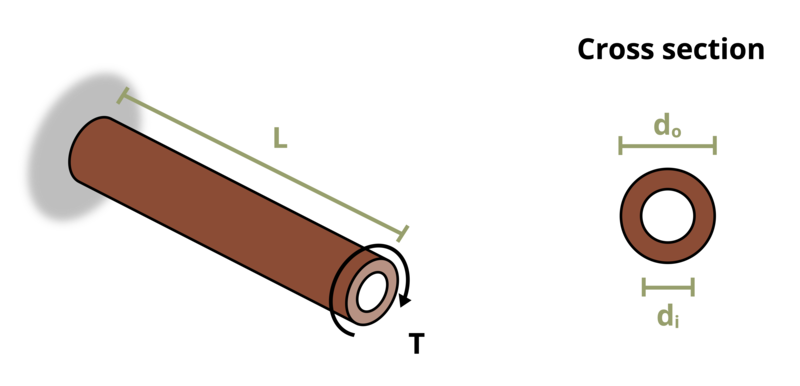
\includegraphics[keepaspectratio]{images/266.png}}

}

\caption{Figure 1: A hollow copper rod is fixed to a wall at one end and
a torque is applied}

\end{figure}%

{[}Problem adapted from © Kurt Gramoll CC BY NC-SA 4.0{]}

\begin{Shaded}
\begin{Highlighting}[]
\NormalTok{\#| standalone: true}
\NormalTok{\#| viewerHeight: 600}
\NormalTok{\#| components: [viewer]}

\NormalTok{from shiny import App, render, ui, reactive}
\NormalTok{import random}
\NormalTok{import asyncio}
\NormalTok{import io}
\NormalTok{import math}
\NormalTok{import string}
\NormalTok{from datetime import datetime}
\NormalTok{from pathlib import Path}

\NormalTok{def generate\_random\_letters(length):}
\NormalTok{    \# Generate a random string of letters of specified length}
\NormalTok{    return \textquotesingle{}\textquotesingle{}.join(random.choice(string.ascii\_lowercase) for \_ in range(length)) }

\NormalTok{problem\_ID="266"}
\NormalTok{L=reactive.Value("\_\_")}
\NormalTok{do=reactive.Value("\_\_")}
\NormalTok{di=reactive.Value("\_\_")}
\NormalTok{angle=(reactive.Value("\_\_"))}
\NormalTok{E = 110}
\NormalTok{v = 0.33}


\NormalTok{attempts=["Timestamp,Attempt,Answer,Feedback\textbackslash{}n"]}

\NormalTok{app\_ui = ui.page\_fluid(}
\NormalTok{    \#ui.markdown("**Please enter your ID number from your instructor and click to generate your problem**"),}
\NormalTok{    \#ui.input\_text("ID","", placeholder="Enter ID Number Here"),}
\NormalTok{    \#ui.input\_action\_button("generate\_problem", "Generate Problem", class\_="btn{-}primary"),}
\NormalTok{    ui.markdown("**Problem Statement**"),}
\NormalTok{    ui.output\_ui("ui\_problem\_statement"),}
\NormalTok{    ui.input\_text("answer","Your Answer in units of kN{-}m", placeholder="Please enter your answer"),}
\NormalTok{    ui.input\_action\_button("submit", "Check Answer", class\_="btn{-}primary"),}
\NormalTok{    \#ui.download\_button("download", "Download File to Submit", class\_="btn{-}success"),}
\NormalTok{)}


\NormalTok{def server(input, output, session):}
\NormalTok{    \# Initialize a counter for attempts}
\NormalTok{    attempt\_counter = reactive.Value(0)}

\NormalTok{    @output}
\NormalTok{    @render.ui}
\NormalTok{    def ui\_problem\_statement():}
\NormalTok{        randomize\_vars()}
\NormalTok{        return[ui.markdown(f"A hollow copper rod (E = 110 GPa, v = 0.33) is subjected to torque T as shown. If length L = \{L()\} m, outer diameter d\textless{}sub\textgreater{}o\textless{}/sub\textgreater{} = \{do()\} mm, and inner diameter d\textless{}sub\textgreater{}i\textless{}/sub\textgreater{} = \{di()\} mm, determine torque T if the rod twists \{angle()\}° .")]}
    
\NormalTok{    \#@reactive.Effect}
\NormalTok{    \#@reactive.event(input.generate\_problem)}
\NormalTok{    def randomize\_vars():}
\NormalTok{        random.seed(101)}
\NormalTok{        L.set(random.randrange(5, 30, 1)/10)}
\NormalTok{        do.set(random.randrange(50, 200, 1))}
\NormalTok{        di.set(round(do()/2, 2))}
\NormalTok{        angle.set(random.randrange(1, 10, 1))}
        
\NormalTok{    @reactive.Effect}
\NormalTok{    @reactive.event(input.submit)}
\NormalTok{    def \_():}
\NormalTok{        attempt\_counter.set(attempt\_counter() + 1)  \# Increment the attempt counter on each submission.}
\NormalTok{        G = E*10**9/(2*(1+v))}
\NormalTok{        J = (math.pi/2)*((do()/2000)**4 {-}(di()/2000)**4 )}
\NormalTok{        instr= ((math.radians(angle())*G*J)/L())/10**3}
\NormalTok{        if math.isclose(float(input.answer()), instr, rel\_tol=0.01):}
\NormalTok{            check = "*Correct*"}
\NormalTok{            correct\_indicator = "JL"}
\NormalTok{        else:}
\NormalTok{            check = "*Not Correct.*"}
\NormalTok{            correct\_indicator = "JG"}

\NormalTok{        \# Generate random parts for the encoded attempt.}
\NormalTok{        random\_start = generate\_random\_letters(4)}
\NormalTok{        random\_middle = generate\_random\_letters(4)}
\NormalTok{        random\_end = generate\_random\_letters(4)}
\NormalTok{        \#encoded\_attempt = f"\{random\_start\}\{problem\_ID\}{-}\{random\_middle\}\{attempt\_counter()\}\{correct\_indicator\}{-}\{random\_end\}\{input.ID()\}"}

\NormalTok{        \# Store the most recent encoded attempt in a reactive value so it persists across submissions}
\NormalTok{        \#session.encoded\_attempt = reactive.Value(encoded\_attempt)}

\NormalTok{        \# Append the attempt data to the attempts list without the encoded attempt}
\NormalTok{        attempts.append(f"\{datetime.now()\}, \{attempt\_counter()\}, \{input.answer()\}, \{check\}\textbackslash{}n")}

\NormalTok{        \# Show feedback to the user.}
\NormalTok{        feedback = ui.markdown(f"Your answer of \{input.answer()\} is \{check\}.")}
\NormalTok{        m = ui.modal(}
\NormalTok{            feedback,}
\NormalTok{            title="Feedback",}
\NormalTok{            easy\_close=True}
\NormalTok{        )}
\NormalTok{        ui.modal\_show(m)}

\NormalTok{    \#@render.download(filename=lambda: f"Problem\_Log{-}\{problem\_ID\}{-}\{input.ID()\}.csv")}
\NormalTok{    async def download():}
\NormalTok{        \# Start the CSV with the encoded attempt (without label)}
\NormalTok{        final\_encoded = session.encoded\_attempt() if session.encoded\_attempt is not None else "No attempts"}
\NormalTok{        yield f"\{final\_encoded\}\textbackslash{}n\textbackslash{}n"}
        
\NormalTok{        \# Write the header for the remaining CSV data once}
\NormalTok{        yield "Timestamp,Attempt,Answer,Feedback\textbackslash{}n"}
        
\NormalTok{        \# Write the attempts data, ensure that the header from the attempts list is not written again}
\NormalTok{        for attempt in attempts[1:]:  \# Skip the first element which is the header}
\NormalTok{            await asyncio.sleep(0.25)  \# This delay may not be necessary; adjust as needed}
\NormalTok{            yield attempt}


\NormalTok{\# App installation}
\NormalTok{app = App(app\_ui, server)}
\end{Highlighting}
\end{Shaded}

\chapter*{Problem 6.12 - Torsional
Deformation}\label{problem-6.12---torsional-deformation}
\addcontentsline{toc}{chapter}{Problem 6.12 - Torsional Deformation}

\markboth{Problem 6.12 - Torsional Deformation}{Problem 6.12 - Torsional
Deformation}

\begin{figure}[H]

{\centering \pandocbounded{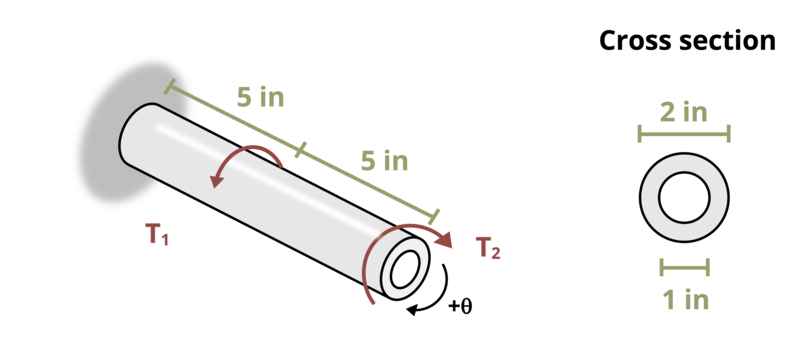
\includegraphics[keepaspectratio]{images/268.png}}

}

\caption{Figure 1: A bar is attached to a wall.}

\end{figure}%

{[}Problem adapted from © Kurt Gramoll CC BY NC-SA 4.0{]}

\begin{Shaded}
\begin{Highlighting}[]
\NormalTok{\#| standalone: true}
\NormalTok{\#| viewerHeight: 600}
\NormalTok{\#| components: [viewer]}

\NormalTok{from shiny import App, render, ui, reactive}
\NormalTok{import random}
\NormalTok{import asyncio}
\NormalTok{import io}
\NormalTok{import math}
\NormalTok{import string}
\NormalTok{from datetime import datetime}
\NormalTok{from pathlib import Path}

\NormalTok{def generate\_random\_letters(length):}
\NormalTok{    \# Generate a random string of letters of specified length}
\NormalTok{    return \textquotesingle{}\textquotesingle{}.join(random.choice(string.ascii\_lowercase) for \_ in range(length)) }

\NormalTok{problem\_ID="268"}
\NormalTok{T1=reactive.Value("\_\_")}
\NormalTok{angle=reactive.Value("\_\_")}
\NormalTok{G=reactive.Value("\_\_")}

\NormalTok{attempts=["Timestamp,Attempt,Answer,Feedback\textbackslash{}n"]}

\NormalTok{app\_ui = ui.page\_fluid(}
\NormalTok{    \#ui.markdown("**Please enter your ID number from your instructor and click to generate your problem**"),}
\NormalTok{    \#ui.input\_text("ID","", placeholder="Enter ID Number Here"),}
\NormalTok{    \#ui.input\_action\_button("generate\_problem", "Generate Problem", class\_="btn{-}primary"),}
\NormalTok{    ui.markdown("**Problem Statement**"),}
\NormalTok{    ui.output\_ui("ui\_problem\_statement"),}
\NormalTok{    ui.input\_text("answer","Your Answer in units of ft{-}lb", placeholder="Please enter your answer"),}
\NormalTok{    ui.input\_action\_button("submit", "Check Answer", class\_="btn{-}primary"),}
\NormalTok{    \#ui.download\_button("download", "Download File to Submit", class\_="btn{-}success"),}
\NormalTok{)}


\NormalTok{def server(input, output, session):}
\NormalTok{    \# Initialize a counter for attempts}
\NormalTok{    attempt\_counter = reactive.Value(0)}

\NormalTok{    @output}
\NormalTok{    @render.ui}
\NormalTok{    def ui\_problem\_statement():}
\NormalTok{        randomize\_vars()}
\NormalTok{        return[ui.markdown(f"A bar with a shear modulus G = \{G()\} x 10\textless{}sup\textgreater{}6\textless{}/sup\textgreater{} psi is subjected to torques T\textless{}sub\textgreater{}1\textless{}/sub\textgreater{} = \{T1()\} lb{-}ft at its center and T\textless{}sub\textgreater{}2\textless{}/sub\textgreater{} at its free end. The inner diamter is 1 in and the outer diameter is 2 in and the total length of the bar is 10 in. If the rotation of the rod at its free end is θ =  \{angle()\}° clockwise, what is the magnitude of torque T\textless{}sub\textgreater{}2\textless{}/sub\textgreater{}?")]}
    
\NormalTok{    \#@reactive.Effect}
\NormalTok{    \#@reactive.event(input.generate\_problem)}
\NormalTok{    def randomize\_vars():}
\NormalTok{        random.seed(101)}
\NormalTok{        G.set(random.randrange(90, 130, 1)/10)}
\NormalTok{        T1.set(random.randrange(1000, 5000, 100))}
\NormalTok{        angle.set(random.randrange(10, 50, 1)/10)}
        
\NormalTok{    @reactive.Effect}
\NormalTok{    @reactive.event(input.submit)}
\NormalTok{    def \_():}
\NormalTok{        attempt\_counter.set(attempt\_counter() + 1)  \# Increment the attempt counter on each submission.}
\NormalTok{        ro = 2/2}
\NormalTok{        ri = 1/2}
\NormalTok{        J = math.pi/2*(ro**4{-}ri**4)}
\NormalTok{        L1 = 10/2}
\NormalTok{        L2 = 10/2}
\NormalTok{        instr= abs((angle()*math.pi/180*G()*10**6*J+T1()*12*L1)/(L1+L2)/12)}
\NormalTok{        if math.isclose(float(input.answer()), instr, rel\_tol=0.01):}
\NormalTok{            check = "*Correct*"}
\NormalTok{            correct\_indicator = "JL"}
\NormalTok{        else:}
\NormalTok{            check = "*Not Correct.*"}
\NormalTok{            correct\_indicator = "JG"}

\NormalTok{        \# Generate random parts for the encoded attempt.}
\NormalTok{        random\_start = generate\_random\_letters(4)}
\NormalTok{        random\_middle = generate\_random\_letters(4)}
\NormalTok{        random\_end = generate\_random\_letters(4)}
\NormalTok{        \#encoded\_attempt = f"\{random\_start\}\{problem\_ID\}{-}\{random\_middle\}\{attempt\_counter()\}\{correct\_indicator\}{-}\{random\_end\}\{input.ID()\}"}

\NormalTok{        \# Store the most recent encoded attempt in a reactive value so it persists across submissions}
\NormalTok{        \#session.encoded\_attempt = reactive.Value(encoded\_attempt)}

\NormalTok{        \# Append the attempt data to the attempts list without the encoded attempt}
\NormalTok{        attempts.append(f"\{datetime.now()\}, \{attempt\_counter()\}, \{input.answer()\}, \{check\}\textbackslash{}n")}

\NormalTok{        \# Show feedback to the user.}
\NormalTok{        feedback = ui.markdown(f"Your answer of \{input.answer()\} is \{check\}.")}
\NormalTok{        m = ui.modal(}
\NormalTok{            feedback,}
\NormalTok{            title="Feedback",}
\NormalTok{            easy\_close=True}
\NormalTok{        )}
\NormalTok{        ui.modal\_show(m)}

\NormalTok{    \#@render.download(filename=lambda: f"Problem\_Log{-}\{problem\_ID\}{-}\{input.ID()\}.csv")}
\NormalTok{    async def download():}
\NormalTok{        \# Start the CSV with the encoded attempt (without label)}
\NormalTok{        final\_encoded = session.encoded\_attempt() if session.encoded\_attempt is not None else "No attempts"}
\NormalTok{        yield f"\{final\_encoded\}\textbackslash{}n\textbackslash{}n"}
        
\NormalTok{        \# Write the header for the remaining CSV data once}
\NormalTok{        yield "Timestamp,Attempt,Answer,Feedback\textbackslash{}n"}
        
\NormalTok{        \# Write the attempts data, ensure that the header from the attempts list is not written again}
\NormalTok{        for attempt in attempts[1:]:  \# Skip the first element which is the header}
\NormalTok{            await asyncio.sleep(0.25)  \# This delay may not be necessary; adjust as needed}
\NormalTok{            yield attempt}

\NormalTok{\# App installation}
\NormalTok{app = App(app\_ui, server)}
\end{Highlighting}
\end{Shaded}

\chapter*{Problem 6.13 - Torsional
Deformation}\label{problem-6.13---torsional-deformation}
\addcontentsline{toc}{chapter}{Problem 6.13 - Torsional Deformation}

\markboth{Problem 6.13 - Torsional Deformation}{Problem 6.13 - Torsional
Deformation}

\pandocbounded{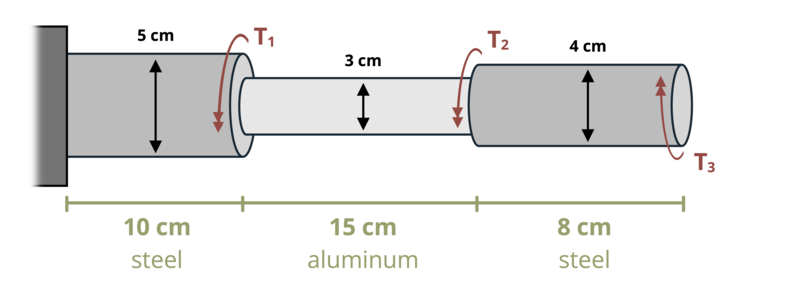
\includegraphics[keepaspectratio]{images/269.png}}
{[}Problem adapted from © Kurt Gramoll CC BY NC-SA 4.0{]}

\begin{Shaded}
\begin{Highlighting}[]
\NormalTok{\#| standalone: true}
\NormalTok{\#| viewerHeight: 600}
\NormalTok{\#| components: [viewer]}

\NormalTok{from shiny import App, render, ui, reactive}
\NormalTok{import random}
\NormalTok{import asyncio}
\NormalTok{import io}
\NormalTok{import math}
\NormalTok{import string}
\NormalTok{from datetime import datetime}
\NormalTok{from pathlib import Path}

\NormalTok{def generate\_random\_letters(length):}
\NormalTok{    \# Generate a random string of letters of specified length}
\NormalTok{    return \textquotesingle{}\textquotesingle{}.join(random.choice(string.ascii\_lowercase) for \_ in range(length)) }

\NormalTok{problem\_ID="269"}
\NormalTok{T1=reactive.Value("\_\_")}
\NormalTok{T2=reactive.Value("\_\_")}
\NormalTok{T3=reactive.Value("\_\_")}
\NormalTok{Gs=77}
\NormalTok{Ga=27}

\NormalTok{attempts=["Timestamp,Attempt,Answer,Feedback\textbackslash{}n"]}

\NormalTok{app\_ui = ui.page\_fluid(}
\NormalTok{    \#ui.markdown("**Please enter your ID number from your instructor and click to generate your problem**"),}
\NormalTok{    \#ui.input\_text("ID","", placeholder="Enter ID Number Here"),}
\NormalTok{    \#ui.input\_action\_button("generate\_problem", "Generate Problem", class\_="btn{-}primary"),}
\NormalTok{    ui.markdown("**Problem Statement**"),}
\NormalTok{    ui.output\_ui("ui\_problem\_statement"),}
\NormalTok{    ui.input\_text("answer","Your Answer in units of degrees", placeholder="Please enter your answer"),}
\NormalTok{    ui.input\_action\_button("submit", "Check Answer", class\_="btn{-}primary"),}
\NormalTok{    \#ui.download\_button("download", "Download File to Submit", class\_="btn{-}success"),}
\NormalTok{)}


\NormalTok{def server(input, output, session):}
\NormalTok{    \# Initialize a counter for attempts}
\NormalTok{    attempt\_counter = reactive.Value(0)}

\NormalTok{    @output}
\NormalTok{    @render.ui}
\NormalTok{    def ui\_problem\_statement():}
\NormalTok{        randomize\_vars()}
\NormalTok{        return[ui.markdown(f"Three moments are applied to the system of cylinders as shown. Assume T\textless{}sub\textgreater{}1\textless{}/sub\textgreater{} = \{T1()\} kN{-}m, T\textless{}sub\textgreater{}2\textless{}/sub\textgreater{} = \{T2()\} kN{-}m, and T\textless{}sub\textgreater{}3\textless{}/sub\textgreater{} = \{T3()\} kN{-}m. If G\textless{}sub\textgreater{}steel\textless{}/sub\textgreater{} = 77 GPa and G\textless{}sub\textgreater{}aluminum\textless{}/sub\textgreater{} = 27 GPa, determine the total angle of twist at the free end.")]}
    
\NormalTok{    \#@reactive.Effect}
\NormalTok{    \#@reactive.event(input.generate\_problem)}
\NormalTok{    def randomize\_vars():}
\NormalTok{        random.seed(101)}
\NormalTok{        T1.set(random.randrange(20, 100, 1)/10)}
\NormalTok{        T2.set(T1()+random.randrange(20, 100, 1)/10)}
\NormalTok{        T3.set(round(T2()*random.randrange(5, 8, 1)/10, 2))}
        
\NormalTok{    @reactive.Effect}
\NormalTok{    @reactive.event(input.submit)}
\NormalTok{    def \_():}
\NormalTok{        attempt\_counter.set(attempt\_counter() + 1)  \# Increment the attempt counter on each submission.}
\NormalTok{        F1 = T1()+T2(){-}T3()}
\NormalTok{        F2 = T2(){-}T3()}
\NormalTok{        F3 = {-}T3()}
\NormalTok{        J1 = (math.pi/2)*((5/200)**4)}
\NormalTok{        J2 = (math.pi/2)*((3/200)**4)}
\NormalTok{        J3 = (math.pi/2)*((4/200)**4)}
\NormalTok{        instr= ((F1*1000*.1)/(J1*Gs*10**9) + (F2*1000*.15)/(J2*Ga*10**9) + (F3*1000*.08)/(J3*Gs*10**9))*180/math.pi}
\NormalTok{        if math.isclose(float(input.answer()), instr, rel\_tol=0.01):}
\NormalTok{            check = "*Correct*"}
\NormalTok{            correct\_indicator = "JL"}
\NormalTok{        else:}
\NormalTok{            check = "*Not Correct.*"}
\NormalTok{            correct\_indicator = "JG"}

\NormalTok{        \# Generate random parts for the encoded attempt.}
\NormalTok{        random\_start = generate\_random\_letters(4)}
\NormalTok{        random\_middle = generate\_random\_letters(4)}
\NormalTok{        random\_end = generate\_random\_letters(4)}
\NormalTok{        \#encoded\_attempt = f"\{random\_start\}\{problem\_ID\}{-}\{random\_middle\}\{attempt\_counter()\}\{correct\_indicator\}{-}\{random\_end\}\{input.ID()\}"}

\NormalTok{        \# Store the most recent encoded attempt in a reactive value so it persists across submissions}
\NormalTok{        \#session.encoded\_attempt = reactive.Value(encoded\_attempt)}

\NormalTok{        \# Append the attempt data to the attempts list without the encoded attempt}
\NormalTok{        attempts.append(f"\{datetime.now()\}, \{attempt\_counter()\}, \{input.answer()\}, \{check\}\textbackslash{}n")}

\NormalTok{        \# Show feedback to the user.}
\NormalTok{        feedback = ui.markdown(f"Your answer of \{input.answer()\} is \{check\}.")}
\NormalTok{        m = ui.modal(}
\NormalTok{            feedback,}
\NormalTok{            title="Feedback",}
\NormalTok{            easy\_close=True}
\NormalTok{        )}
\NormalTok{        ui.modal\_show(m)}

\NormalTok{    \#@render.download(filename=lambda: f"Problem\_Log{-}\{problem\_ID\}{-}\{input.ID()\}.csv")}
\NormalTok{    async def download():}
\NormalTok{        \# Start the CSV with the encoded attempt (without label)}
\NormalTok{        final\_encoded = session.encoded\_attempt() if session.encoded\_attempt is not None else "No attempts"}
\NormalTok{        yield f"\{final\_encoded\}\textbackslash{}n\textbackslash{}n"}
        
\NormalTok{        \# Write the header for the remaining CSV data once}
\NormalTok{        yield "Timestamp,Attempt,Answer,Feedback\textbackslash{}n"}
        
\NormalTok{        \# Write the attempts data, ensure that the header from the attempts list is not written again}
\NormalTok{        for attempt in attempts[1:]:  \# Skip the first element which is the header}
\NormalTok{            await asyncio.sleep(0.25)  \# This delay may not be necessary; adjust as needed}
\NormalTok{            yield attempt}

\NormalTok{\# App installation}
\NormalTok{app = App(app\_ui, server)}
\end{Highlighting}
\end{Shaded}

\chapter*{Problem 6.14 - Torsional
Deformation}\label{problem-6.14---torsional-deformation}
\addcontentsline{toc}{chapter}{Problem 6.14 - Torsional Deformation}

\markboth{Problem 6.14 - Torsional Deformation}{Problem 6.14 - Torsional
Deformation}

\pandocbounded{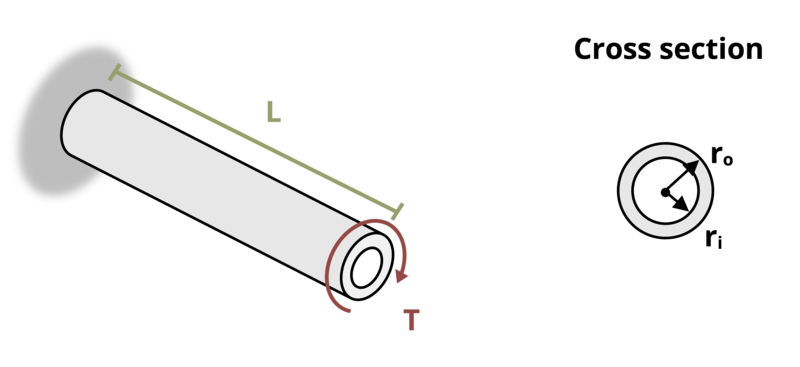
\includegraphics[keepaspectratio]{images/270.png}}
{[}Problem adapted from © Kurt Gramoll CC BY NC-SA 4.0{]}

\begin{Shaded}
\begin{Highlighting}[]
\NormalTok{\#| standalone: true}
\NormalTok{\#| viewerHeight: 600}
\NormalTok{\#| components: [viewer]}

\NormalTok{from shiny import App, render, ui, reactive}
\NormalTok{import random}
\NormalTok{import asyncio}
\NormalTok{import io}
\NormalTok{import math}
\NormalTok{import string}
\NormalTok{from datetime import datetime}
\NormalTok{from pathlib import Path}

\NormalTok{def generate\_random\_letters(length):}
\NormalTok{    \# Generate a random string of letters of specified length}
\NormalTok{    return \textquotesingle{}\textquotesingle{}.join(random.choice(string.ascii\_lowercase) for \_ in range(length)) }

\NormalTok{problem\_ID="270"}
\NormalTok{L=reactive.Value("\_\_")}
\NormalTok{ro=reactive.Value("\_\_")}
\NormalTok{T=reactive.Value("\_\_")}
\NormalTok{G=reactive.Value("\_\_")}
\NormalTok{stress=reactive.Value("\_\_")}

\NormalTok{attempts=["Timestamp,Attempt,Answer,Feedback\textbackslash{}n"]}

\NormalTok{app\_ui = ui.page\_fluid(}
\NormalTok{    \#ui.markdown("**Please enter your ID number from your instructor and click to generate your problem**"),}
\NormalTok{    \#ui.input\_text("ID","", placeholder="Enter ID Number Here"),}
\NormalTok{    \#ui.input\_action\_button("generate\_problem", "Generate Problem", class\_="btn{-}primary"),}
\NormalTok{    ui.markdown("**Problem Statement**"),}
\NormalTok{    ui.output\_ui("ui\_problem\_statement"),}
\NormalTok{    ui.input\_text("answer","Your Answer in units of mm", placeholder="Please enter your answer"),}
\NormalTok{    ui.input\_action\_button("submit", "Check Answer", class\_="btn{-}primary"),}
\NormalTok{    \#ui.download\_button("download", "Download File to Submit", class\_="btn{-}success"),}
\NormalTok{)}

\NormalTok{def server(input, output, session):}
\NormalTok{    \# Initialize a counter for attempts}
\NormalTok{    attempt\_counter = reactive.Value(0)}

\NormalTok{    @output}
\NormalTok{    @render.ui}
\NormalTok{    def ui\_problem\_statement():}
\NormalTok{        randomize\_vars()}
\NormalTok{        return[ui.markdown(f"A circular rod of length L = \{L()\} mm, outer radius r\textless{}sub\textgreater{}o\textless{}/sub\textgreater{} = \{ro()\} mm, and unknown inner radius r\textless{}sub\textgreater{}i\textless{}/sub\textgreater{} has a shear modulus G = \{G()\} GPa. The rod is subjected to torque T = \{T()\} kN{-}m at the free end. If the angle of twist must not exceed 2° and the shear stress must not exceed \{stress()\} MPa, what is the minimum required inner radius?")]}
    
\NormalTok{    \#@reactive.Effect}
\NormalTok{    \#@reactive.event(input.generate\_problem)}
\NormalTok{    def randomize\_vars():}
\NormalTok{        random.seed(101)}
\NormalTok{        L.set(random.randrange(250, 500, 10))}
\NormalTok{        ro.set(random.randrange(55, 75, 1))}
\NormalTok{        G.set(random.randrange(60, 100, 1))}
\NormalTok{        T.set(random.randrange(10, 100, 1)/10)}
\NormalTok{        stress.set(random.randrange(75, 150, 1))}
        
\NormalTok{    @reactive.Effect}
\NormalTok{    @reactive.event(input.submit)}
\NormalTok{    def \_():}
\NormalTok{        attempt\_counter.set(attempt\_counter() + 1)  \# Increment the attempt counter on each submission.}
\NormalTok{        r1= ((ro()/1000)**4{-}(2*T()*1000*ro()/1000/(math.pi*stress()*10**6)))**0.25*1000}
\NormalTok{        r2 = ((ro()/1000)**4{-}(2*T()*1000*L()/1000/(math.pi*G()*10**9*2*math.pi/180)))**0.25*1000}
\NormalTok{        if r1\textgreater{}r2:}
\NormalTok{            instr = r2}
\NormalTok{        else:}
\NormalTok{            instr = r1}
\NormalTok{        if math.isclose(float(input.answer()), instr, rel\_tol=0.01):}
\NormalTok{            check = "*Correct*"}
\NormalTok{            correct\_indicator = "JL"}
\NormalTok{        else:}
\NormalTok{            check = "*Not Correct.*"}
\NormalTok{            correct\_indicator = "JG"}

\NormalTok{        \# Generate random parts for the encoded attempt.}
\NormalTok{        random\_start = generate\_random\_letters(4)}
\NormalTok{        random\_middle = generate\_random\_letters(4)}
\NormalTok{        random\_end = generate\_random\_letters(4)}
\NormalTok{        \#encoded\_attempt = f"\{random\_start\}\{problem\_ID\}{-}\{random\_middle\}\{attempt\_counter()\}\{correct\_indicator\}{-}\{random\_end\}\{input.ID()\}"}

\NormalTok{        \# Store the most recent encoded attempt in a reactive value so it persists across submissions}
\NormalTok{        \#session.encoded\_attempt = reactive.Value(encoded\_attempt)}

\NormalTok{        \# Append the attempt data to the attempts list without the encoded attempt}
\NormalTok{        attempts.append(f"\{datetime.now()\}, \{attempt\_counter()\}, \{input.answer()\}, \{check\}\textbackslash{}n")}

\NormalTok{        \# Show feedback to the user.}
\NormalTok{        feedback = ui.markdown(f"Your answer of \{input.answer()\} is \{check\}.")}
\NormalTok{        m = ui.modal(}
\NormalTok{            feedback,}
\NormalTok{            title="Feedback",}
\NormalTok{            easy\_close=True}
\NormalTok{        )}
\NormalTok{        ui.modal\_show(m)}

\NormalTok{    \#@render.download(filename=lambda: f"Problem\_Log{-}\{problem\_ID\}{-}\{input.ID()\}.csv")}
\NormalTok{    async def download():}
\NormalTok{        \# Start the CSV with the encoded attempt (without label)}
\NormalTok{        final\_encoded = session.encoded\_attempt() if session.encoded\_attempt is not None else "No attempts"}
\NormalTok{        yield f"\{final\_encoded\}\textbackslash{}n\textbackslash{}n"}
        
\NormalTok{        \# Write the header for the remaining CSV data once}
\NormalTok{        yield "Timestamp,Attempt,Answer,Feedback\textbackslash{}n"}
        
\NormalTok{        \# Write the attempts data, ensure that the header from the attempts list is not written again}
\NormalTok{        for attempt in attempts[1:]:  \# Skip the first element which is the header}
\NormalTok{            await asyncio.sleep(0.25)  \# This delay may not be necessary; adjust as needed}
\NormalTok{            yield attempt}

\NormalTok{\# App installation}
\NormalTok{app = App(app\_ui, server)}
\end{Highlighting}
\end{Shaded}

\chapter*{Problem 6.15 - Torsional
Deformation}\label{problem-6.15---torsional-deformation}
\addcontentsline{toc}{chapter}{Problem 6.15 - Torsional Deformation}

\markboth{Problem 6.15 - Torsional Deformation}{Problem 6.15 - Torsional
Deformation}

\begin{figure}[H]

{\centering \pandocbounded{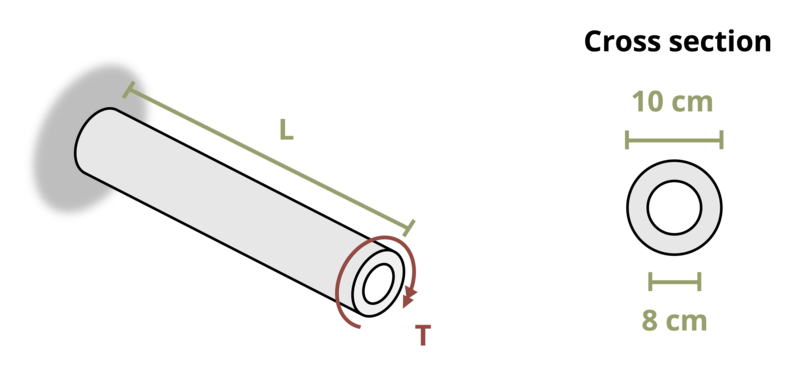
\includegraphics[keepaspectratio]{images/274.png}}

}

\caption{Figure 1: A hollow circualr rod is attached to a wall and
subjected to a torque at the free end.}

\end{figure}%

{[}Problem adapted from © Kurt Gramoll CC BY NC-SA 4.0{]}

\begin{Shaded}
\begin{Highlighting}[]
\NormalTok{\#| standalone: true}
\NormalTok{\#| viewerHeight: 600}
\NormalTok{\#| components: [viewer]}

\NormalTok{from shiny import App, render, ui, reactive}
\NormalTok{import random}
\NormalTok{import asyncio}
\NormalTok{import io}
\NormalTok{import math}
\NormalTok{import string}
\NormalTok{from datetime import datetime}
\NormalTok{from pathlib import Path}

\NormalTok{def generate\_random\_letters(length):}
\NormalTok{    \# Generate a random string of letters of specified length}
\NormalTok{    return \textquotesingle{}\textquotesingle{}.join(random.choice(string.ascii\_lowercase) for \_ in range(length)) }

\NormalTok{problem\_ID="274"}
\NormalTok{T=reactive.Value("\_\_")}
\NormalTok{x=reactive.Value("\_\_")}
\NormalTok{G=reactive.Value("\_\_")}
\NormalTok{L=reactive.Value("\_\_")}

\NormalTok{attempts=["Timestamp,Attempt,Answer,Feedback\textbackslash{}n"]}

\NormalTok{app\_ui = ui.page\_fluid(}
\NormalTok{    \#ui.markdown("**Please enter your ID number from your instructor and click to generate your problem**"),}
\NormalTok{    \#ui.input\_text("ID","", placeholder="Enter ID Number Here"),}
\NormalTok{    \#ui.input\_action\_button("generate\_problem", "Generate Problem", class\_="btn{-}primary"),}
\NormalTok{    ui.markdown("**Problem Statement**"),}
\NormalTok{    ui.output\_ui("ui\_problem\_statement"),}
\NormalTok{    ui.input\_text("answer","Your Answer in units of degrees", placeholder="Please enter your answer"),}
\NormalTok{    ui.input\_action\_button("submit", "Check Answer", class\_="btn{-}primary"),}
\NormalTok{    \#ui.download\_button("download", "Download File to Submit", class\_="btn{-}success"),}
\NormalTok{)}

\NormalTok{def server(input, output, session):}
\NormalTok{    \# Initialize a counter for attempts}
\NormalTok{    attempt\_counter = reactive.Value(0)}

\NormalTok{    @output}
\NormalTok{    @render.ui}
\NormalTok{    def ui\_problem\_statement():}
\NormalTok{        randomize\_vars()}
\NormalTok{        return[ui.markdown(f"A hollow circular rod is attached to a wall and subjected to a torque T = \{T()\} kN{-}m at the free end.The rod has inner diameter 8 cm and outer diameter 10 cm.  Determine the angle of twist at x = \{x()\} mm. Assume G = \{G()\} GPa and L = \{L()\} mm.")]}
    
\NormalTok{    \#@reactive.Effect}
\NormalTok{    \#@reactive.event(input.generate\_problem)}
\NormalTok{    def randomize\_vars():}
\NormalTok{        random.seed(101)}
\NormalTok{        T.set(random.randrange(20, 200, 1)/10)}
\NormalTok{        G.set(random.randrange(30, 60, 1))}
\NormalTok{        L.set(random.randrange(300, 800, 10))}
\NormalTok{        x.set(L()*random.randrange(2,7,1)/10)}
        
\NormalTok{    @reactive.Effect}
\NormalTok{    @reactive.event(input.submit)}
\NormalTok{    def \_():}
\NormalTok{        attempt\_counter.set(attempt\_counter() + 1)  \# Increment the attempt counter on each submission.}
\NormalTok{        J = (math.pi/2)*((10/200)**4 {-} (8/200)**4)}
\NormalTok{        angle = (T()*1000*x()/1000)/(G()*10**9*J)}
\NormalTok{        instr= math.degrees(angle)}
\NormalTok{        if math.isclose(float(input.answer()), instr, rel\_tol=0.01):}
\NormalTok{            check = "*Correct*"}
\NormalTok{            correct\_indicator = "JL"}
\NormalTok{        else:}
\NormalTok{            check = "*Not Correct.*"}
\NormalTok{            correct\_indicator = "JG"}

\NormalTok{        \# Generate random parts for the encoded attempt.}
\NormalTok{        random\_start = generate\_random\_letters(4)}
\NormalTok{        random\_middle = generate\_random\_letters(4)}
\NormalTok{        random\_end = generate\_random\_letters(4)}
\NormalTok{        \#encoded\_attempt = f"\{random\_start\}\{problem\_ID\}{-}\{random\_middle\}\{attempt\_counter()\}\{correct\_indicator\}{-}\{random\_end\}\{input.ID()\}"}

\NormalTok{        \# Store the most recent encoded attempt in a reactive value so it persists across submissions}
\NormalTok{        \#session.encoded\_attempt = reactive.Value(encoded\_attempt)}

\NormalTok{        \# Append the attempt data to the attempts list without the encoded attempt}
\NormalTok{        attempts.append(f"\{datetime.now()\}, \{attempt\_counter()\}, \{input.answer()\}, \{check\}\textbackslash{}n")}

\NormalTok{        \# Show feedback to the user.}
\NormalTok{        feedback = ui.markdown(f"Your answer of \{input.answer()\} is \{check\}.")}
\NormalTok{        m = ui.modal(}
\NormalTok{            feedback,}
\NormalTok{            title="Feedback",}
\NormalTok{            easy\_close=True}
\NormalTok{        )}
\NormalTok{        ui.modal\_show(m)}

\NormalTok{    \#@render.download(filename=lambda: f"Problem\_Log{-}\{problem\_ID\}{-}\{input.ID()\}.csv")}
\NormalTok{    async def download():}
\NormalTok{        \# Start the CSV with the encoded attempt (without label)}
\NormalTok{        final\_encoded = session.encoded\_attempt() if session.encoded\_attempt is not None else "No attempts"}
\NormalTok{        yield f"\{final\_encoded\}\textbackslash{}n\textbackslash{}n"}
        
\NormalTok{        \# Write the header for the remaining CSV data once}
\NormalTok{        yield "Timestamp,Attempt,Answer,Feedback\textbackslash{}n"}
        
\NormalTok{        \# Write the attempts data, ensure that the header from the attempts list is not written again}
\NormalTok{        for attempt in attempts[1:]:  \# Skip the first element which is the header}
\NormalTok{            await asyncio.sleep(0.25)  \# This delay may not be necessary; adjust as needed}
\NormalTok{            yield attempt}

\NormalTok{\# App installation}
\NormalTok{app = App(app\_ui, server)}
\end{Highlighting}
\end{Shaded}

\chapter*{Problem 6.16 - Torsional
Deformation}\label{problem-6.16---torsional-deformation}
\addcontentsline{toc}{chapter}{Problem 6.16 - Torsional Deformation}

\markboth{Problem 6.16 - Torsional Deformation}{Problem 6.16 - Torsional
Deformation}

\pandocbounded{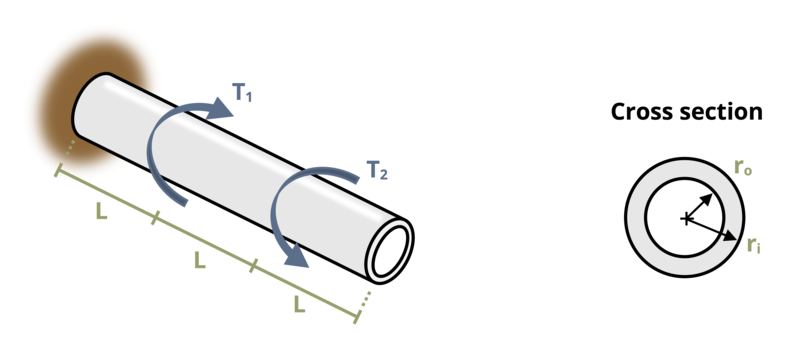
\includegraphics[keepaspectratio]{images/275.png}}
{[}Problem adapted from © Kurt Gramoll CC BY NC-SA 4.0{]}

\begin{Shaded}
\begin{Highlighting}[]
\NormalTok{\#| standalone: true}
\NormalTok{\#| viewerHeight: 600}
\NormalTok{\#| components: [viewer]}

\NormalTok{from shiny import App, render, ui, reactive}
\NormalTok{import random}
\NormalTok{import asyncio}
\NormalTok{import io}
\NormalTok{import math}
\NormalTok{import string}
\NormalTok{from datetime import datetime}
\NormalTok{from pathlib import Path}

\NormalTok{def generate\_random\_letters(length):}
\NormalTok{    \# Generate a random string of letters of specified length}
\NormalTok{    return \textquotesingle{}\textquotesingle{}.join(random.choice(string.ascii\_lowercase) for \_ in range(length))}

\NormalTok{problem\_ID="275"}
\NormalTok{T1=reactive.Value("\_\_")}
\NormalTok{T2=reactive.Value("\_\_")}
\NormalTok{ro=reactive.Value("\_\_")}
\NormalTok{ri=reactive.Value("\_\_")}
\NormalTok{L=reactive.Value("\_\_")}

\NormalTok{attempts=["Timestamp,Attempt,Answer,Feedback\textbackslash{}n"]}

\NormalTok{app\_ui = ui.page\_fluid(}
\NormalTok{    \#ui.markdown("**Please enter your ID number from your instructor and click to generate your problem**"),}
\NormalTok{    \#ui.input\_text("ID","", placeholder="Enter ID Number Here"),}
\NormalTok{    \#ui.input\_action\_button("generate\_problem", "Generate Problem", class\_="btn{-}primary"),}
\NormalTok{    ui.markdown("**Problem Statement**"),}
\NormalTok{    ui.output\_ui("ui\_problem\_statement"),}
\NormalTok{    ui.input\_text("answer","Your Answer in units of rad", placeholder="Please enter your answer"),}
\NormalTok{    ui.input\_action\_button("submit", "Check Answer", class\_="btn{-}primary"),}
\NormalTok{    \#ui.download\_button("download", "Download File to Submit", class\_="btn{-}success"),}
\NormalTok{)}

\NormalTok{def server(input, output, session):}
\NormalTok{    \# Initialize a counter for attempts}
\NormalTok{    attempt\_counter = reactive.Value(0)}

\NormalTok{    @output}
\NormalTok{    @render.ui}
\NormalTok{    def ui\_problem\_statement():}
\NormalTok{        randomize\_vars()}
\NormalTok{        return[ui.markdown(f"A rod is subjected to two torques, T\textless{}sub\textgreater{}1\textless{}/sub\textgreater{} = \{T1()\} kip{-}in. and T\textless{}sub\textgreater{}2\textless{}/sub\textgreater{} = \{T2()\} kip{-}in. as shown. The rod is hollow, with outer radius r\textless{}sub\textgreater{}o\textless{}/sub\textgreater{} = \{ro()\} in. and inner radius r\textless{}sub\textgreater{}i\textless{}/sub\textgreater{} = \{ri()\} in. If length L = \{L()\} in., determine the angle of twist at the free end. Assume E = 300 ksi and ν = 0.4.")]}
    
\NormalTok{    \#@reactive.Effect}
\NormalTok{    \#@reactive.event(input.generate\_problem)}
\NormalTok{    def randomize\_vars():}
\NormalTok{        random.seed(101)}
\NormalTok{        T1.set(random.randrange(50,200,1))}
\NormalTok{        T2.set(random.randrange(50,200,1))}
\NormalTok{        ro.set(random.randrange(20,50,1)/10)}
\NormalTok{        ri.set(ro(){-}random.randrange(5,10,1)/10)}
\NormalTok{        L.set(random.randrange(5,20,1))}
    
\NormalTok{    @reactive.Effect}
\NormalTok{    @reactive.event(input.submit)}
\NormalTok{    def \_():}
\NormalTok{        attempt\_counter.set(attempt\_counter() + 1)  \# Increment the attempt counter on each submission.}
\NormalTok{        G = 300000/(2*1.4)}
\NormalTok{        J = math.pi/2*(ro()**4{-}ri()**4)}
\NormalTok{        theta1 = {-}T1()*1000*L()/(G*J)}
\NormalTok{        theta2 = T2()*1000*2*L()/(G*J)}
\NormalTok{        instr = (theta1+theta2)}
\NormalTok{        if math.isclose(float(input.answer()), instr, rel\_tol=0.01):}
\NormalTok{            check = "*Correct*"}
\NormalTok{            correct\_indicator = "JL"}
\NormalTok{        else:}
\NormalTok{            check = "*Not Correct.*"}
\NormalTok{            correct\_indicator = "JG"}

\NormalTok{        \# Generate random parts for the encoded attempt.}
\NormalTok{        random\_start = generate\_random\_letters(4)}
\NormalTok{        random\_middle = generate\_random\_letters(4)}
\NormalTok{        random\_end = generate\_random\_letters(4)}
\NormalTok{        \#encoded\_attempt = f"\{random\_start\}\{problem\_ID\}{-}\{random\_middle\}\{attempt\_counter()\}\{correct\_indicator\}{-}\{random\_end\}\{input.ID()\}"}

\NormalTok{        \# Store the most recent encoded attempt in a reactive value so it persists across submissions}
\NormalTok{        \#session.encoded\_attempt = reactive.Value(encoded\_attempt)}

\NormalTok{        \# Append the attempt data to the attempts list without the encoded attempt}
\NormalTok{        attempts.append(f"\{datetime.now()\}, \{attempt\_counter()\}, \{input.answer()\}, \{check\}\textbackslash{}n")}

\NormalTok{        \# Show feedback to the user.}
\NormalTok{        feedback = ui.markdown(f"Your answer of \{input.answer()\} is \{check\}.")}
\NormalTok{        m = ui.modal(}
\NormalTok{            feedback,}
\NormalTok{            title="Feedback",}
\NormalTok{            easy\_close=True}
\NormalTok{        )}
\NormalTok{        ui.modal\_show(m)}

\NormalTok{    \#@render.download(filename=lambda: f"Problem\_Log{-}\{problem\_ID\}{-}\{input.ID()\}.csv")}
\NormalTok{    async def download():}
\NormalTok{        \# Start the CSV with the encoded attempt (without label)}
\NormalTok{        final\_encoded = session.encoded\_attempt() if session.encoded\_attempt is not None else "No attempts"}
\NormalTok{        yield f"\{final\_encoded\}\textbackslash{}n\textbackslash{}n"}
        
\NormalTok{        \# Write the header for the remaining CSV data once}
\NormalTok{        yield "Timestamp,Attempt,Answer,Feedback\textbackslash{}n"}
        
\NormalTok{        \# Write the attempts data, ensure that the header from the attempts list is not written again}
\NormalTok{        for attempt in attempts[1:]:  \# Skip the first element which is the header}
\NormalTok{            await asyncio.sleep(0.25)  \# This delay may not be necessary; adjust as needed}
\NormalTok{            yield attempt}

\NormalTok{\# App installation}
\NormalTok{app = App(app\_ui, server)}
\end{Highlighting}
\end{Shaded}

\chapter*{Problem 6.17 - Torsional
Deformation}\label{problem-6.17---torsional-deformation}
\addcontentsline{toc}{chapter}{Problem 6.17 - Torsional Deformation}

\markboth{Problem 6.17 - Torsional Deformation}{Problem 6.17 - Torsional
Deformation}

\pandocbounded{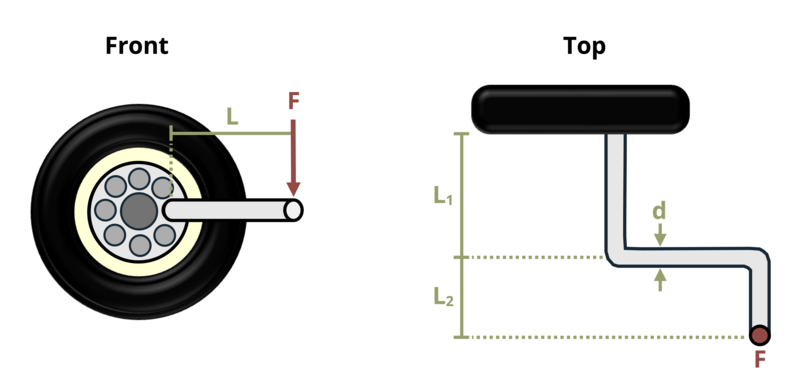
\includegraphics[keepaspectratio]{images/277.png}}
{[}Problem adapted from © Kurt Gramoll CC BY NC-SA 4.0{]}

\begin{Shaded}
\begin{Highlighting}[]
\NormalTok{\#| standalone: true}
\NormalTok{\#| viewerHeight: 600}
\NormalTok{\#| components: [viewer]}

\NormalTok{from shiny import App, render, ui, reactive}
\NormalTok{import random}
\NormalTok{import asyncio}
\NormalTok{import io}
\NormalTok{import math}
\NormalTok{import string}
\NormalTok{from datetime import datetime}
\NormalTok{from pathlib import Path}

\NormalTok{def generate\_random\_letters(length):}
\NormalTok{    \# Generate a random string of letters of specified length}
\NormalTok{    return \textquotesingle{}\textquotesingle{}.join(random.choice(string.ascii\_lowercase) for \_ in range(length))}

\NormalTok{problem\_ID="277"}
\NormalTok{L=reactive.Value("\_\_")}
\NormalTok{d=reactive.Value("\_\_")}
\NormalTok{F=reactive.Value("\_\_")}

\NormalTok{attempts=["Timestamp,Attempt,Answer,Feedback\textbackslash{}n"]}

\NormalTok{app\_ui = ui.page\_fluid(}
\NormalTok{    \#ui.markdown("**Please enter your ID number from your instructor and click to generate your problem**"),}
\NormalTok{    \#ui.input\_text("ID","", placeholder="Enter ID Number Here"),}
\NormalTok{    \#ui.input\_action\_button("generate\_problem", "Generate Problem", class\_="btn{-}primary"),}
\NormalTok{    ui.markdown("**Problem Statement**"),}
\NormalTok{    ui.output\_ui("ui\_problem\_statement"),}
\NormalTok{    ui.input\_text("answer","Your Answer in units of degrees", placeholder="Please enter your answer"),}
\NormalTok{    ui.input\_action\_button("submit", "Check Answer", class\_="btn{-}primary"),}
\NormalTok{    \#ui.download\_button("download", "Download File to Submit", class\_="btn{-}success"),}
\NormalTok{)}

\NormalTok{def server(input, output, session):}
\NormalTok{    \# Initialize a counter for attempts}
\NormalTok{    attempt\_counter = reactive.Value(0)}

\NormalTok{    @output}
\NormalTok{    @render.ui}
\NormalTok{    def ui\_problem\_statement():}
\NormalTok{        randomize\_vars()}
\NormalTok{        return[ui.markdown(f"A tire iron of length L = \{L()\} ft is used to tighten a nut on a tire as shown. The tire iron has diameter d = \{d()\} in, elastic modulus E = 29,000 ksi, and Poisson\textquotesingle{}s ratio ν = 0.29. If load F = \{F()\} lb, determine the angle of twist in the tire iron before the nut rotates.")]}
    
\NormalTok{    \#@reactive.Effect}
\NormalTok{    \#@reactive.event(input.generate\_problem)}
\NormalTok{    def randomize\_vars():}
\NormalTok{        random.seed(101)}
\NormalTok{        L.set(random.randrange(10,25,1)/10)}
\NormalTok{        d.set(random.randrange(25,75,5)/100)}
\NormalTok{        F.set(random.randrange(75,150,1))}
        
\NormalTok{    @reactive.Effect}
\NormalTok{    @reactive.event(input.submit)}
\NormalTok{    def \_():}
\NormalTok{        attempt\_counter.set(attempt\_counter() + 1)  \# Increment the attempt counter on each submission.}
\NormalTok{        T = F()*L()*12}
\NormalTok{        G = 29000000/(2*(1.29))}
\NormalTok{        J = math.pi/2*(d()/2)**4}
\NormalTok{        theta = T*L()*12/(G*J)}
\NormalTok{        instr = theta*180/math.pi}
\NormalTok{        if math.isclose(float(input.answer()), instr, rel\_tol=0.01):}
\NormalTok{            check = "*Correct*"}
\NormalTok{            correct\_indicator = "JL"}
\NormalTok{        else:}
\NormalTok{            check = "*Not Correct.*"}
\NormalTok{            correct\_indicator = "JG"}

\NormalTok{        \# Generate random parts for the encoded attempt.}
\NormalTok{        random\_start = generate\_random\_letters(4)}
\NormalTok{        random\_middle = generate\_random\_letters(4)}
\NormalTok{        random\_end = generate\_random\_letters(4)}
\NormalTok{        \#encoded\_attempt = f"\{random\_start\}\{problem\_ID\}{-}\{random\_middle\}\{attempt\_counter()\}\{correct\_indicator\}{-}\{random\_end\}\{input.ID()\}"}

\NormalTok{        \# Store the most recent encoded attempt in a reactive value so it persists across submissions}
\NormalTok{        \#session.encoded\_attempt = reactive.Value(encoded\_attempt)}

\NormalTok{        \# Append the attempt data to the attempts list without the encoded attempt}
\NormalTok{        attempts.append(f"\{datetime.now()\}, \{attempt\_counter()\}, \{input.answer()\}, \{check\}\textbackslash{}n")}

\NormalTok{        \# Show feedback to the user.}
\NormalTok{        feedback = ui.markdown(f"Your answer of \{input.answer()\} is \{check\}.")}
\NormalTok{        m = ui.modal(}
\NormalTok{            feedback,}
\NormalTok{            title="Feedback",}
\NormalTok{            easy\_close=True}
\NormalTok{        )}
\NormalTok{        ui.modal\_show(m)}

\NormalTok{    \#@render.download(filename=lambda: f"Problem\_Log{-}\{problem\_ID\}{-}\{input.ID()\}.csv")}
\NormalTok{    async def download():}
\NormalTok{        \# Start the CSV with the encoded attempt (without label)}
\NormalTok{        final\_encoded = session.encoded\_attempt() if session.encoded\_attempt is not None else "No attempts"}
\NormalTok{        yield f"\{final\_encoded\}\textbackslash{}n\textbackslash{}n"}
        
\NormalTok{        \# Write the header for the remaining CSV data once}
\NormalTok{        yield "Timestamp,Attempt,Answer,Feedback\textbackslash{}n"}
        
\NormalTok{        \# Write the attempts data, ensure that the header from the attempts list is not written again}
\NormalTok{        for attempt in attempts[1:]:  \# Skip the first element which is the header}
\NormalTok{            await asyncio.sleep(0.25)  \# This delay may not be necessary; adjust as needed}
\NormalTok{            yield attempt}

\NormalTok{\# App installation}
\NormalTok{app = App(app\_ui, server)}
\end{Highlighting}
\end{Shaded}

\chapter*{Problem 6.18 - Torsional
Deformation}\label{problem-6.18---torsional-deformation}
\addcontentsline{toc}{chapter}{Problem 6.18 - Torsional Deformation}

\markboth{Problem 6.18 - Torsional Deformation}{Problem 6.18 - Torsional
Deformation}

\pandocbounded{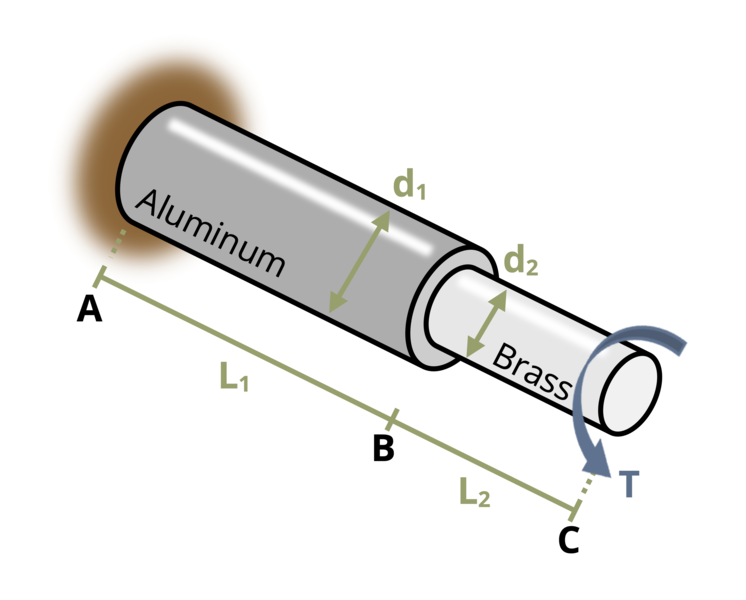
\includegraphics[keepaspectratio]{images/279.png}}
{[}Problem adapted from © Kurt Gramoll CC BY NC-SA 4.0{]}

\begin{Shaded}
\begin{Highlighting}[]
\NormalTok{\#| standalone: true}
\NormalTok{\#| viewerHeight: 600}
\NormalTok{\#| components: [viewer]}

\NormalTok{from shiny import App, render, ui, reactive}
\NormalTok{import random}
\NormalTok{import asyncio}
\NormalTok{import io}
\NormalTok{import math}
\NormalTok{import string}
\NormalTok{from datetime import datetime}
\NormalTok{from pathlib import Path}

\NormalTok{def generate\_random\_letters(length):}
\NormalTok{    \# Generate a random string of letters of specified length}
\NormalTok{    return \textquotesingle{}\textquotesingle{}.join(random.choice(string.ascii\_lowercase) for \_ in range(length))}

\NormalTok{problem\_ID="279"}
\NormalTok{T=reactive.Value("\_\_")}
\NormalTok{L2=reactive.Value("\_\_")}
\NormalTok{L1=reactive.Value("\_\_")}
\NormalTok{d2=reactive.Value("\_\_")}
\NormalTok{d1=reactive.Value("\_\_")}

\NormalTok{attempts=["Timestamp,Attempt,Answer,Feedback\textbackslash{}n"]}

\NormalTok{app\_ui = ui.page\_fluid(}
\NormalTok{    \#ui.markdown("**Please enter your ID number from your instructor and click to generate your problem**"),}
\NormalTok{    \#ui.input\_text("ID","", placeholder="Enter ID Number Here"),}
\NormalTok{    \#ui.input\_action\_button("generate\_problem", "Generate Problem", class\_="btn{-}primary"),}
\NormalTok{    ui.markdown("**Problem Statement**"),}
\NormalTok{    ui.output\_ui("ui\_problem\_statement"),}
\NormalTok{    ui.input\_text("answer","Your Answer in units of degrees", placeholder="Please enter your answer"),}
\NormalTok{    ui.input\_action\_button("submit", "Check Answer", class\_="btn{-}primary"),}
\NormalTok{    \#ui.download\_button("download", "Download File to Submit", class\_="btn{-}success"),}
\NormalTok{)}

\NormalTok{def server(input, output, session):}
\NormalTok{    \# Initialize a counter for attempts}
\NormalTok{    attempt\_counter = reactive.Value(0)}

\NormalTok{    @output}
\NormalTok{    @render.ui}
\NormalTok{    def ui\_problem\_statement():}
\NormalTok{        randomize\_vars()}
\NormalTok{        return[ui.markdown(f"A two part rod made of aluminum (E = 70 GPa, ν = 0.33) and brass (E = 100 GPa, ν = 0.34) is subjected to a torque T = \{T()\} N{-}m at its free end. If length L\textless{}sub\textgreater{}1\textless{}/sub\textgreater{} = \{L1()\} mm and L\textless{}sub\textgreater{}2\textless{}/sub\textgreater{} = \{L2()\} mm, and diameters d\textless{}sub\textgreater{}1\textless{}/sub\textgreater{} = \{d1()\} mm and d\textless{}sub\textgreater{}2\textless{}/sub\textgreater{} = \{d2()\} mm, determine the angle of twist of the free end.")]}
    
\NormalTok{    \#@reactive.Effect}
\NormalTok{    \#@reactive.event(input.generate\_problem)}
\NormalTok{    def randomize\_vars():}
\NormalTok{        random.seed(101)}
\NormalTok{        T.set(random.randrange(250,900,10))}
\NormalTok{        L2.set(random.randrange(200,500,10))}
\NormalTok{        L1.set(round(L2()*1.4,1))}
\NormalTok{        d2.set(random.randrange(30,60,2))}
\NormalTok{        d1.set(d2()*1.5)}
        
\NormalTok{    @reactive.Effect}
\NormalTok{    @reactive.event(input.submit)}
\NormalTok{    def \_():}
\NormalTok{        attempt\_counter.set(attempt\_counter() + 1)  \# Increment the attempt counter on each submission.}
\NormalTok{        Ga = 70*10**9/(2*1.33)}
\NormalTok{        Gb = 100*10**9/(2*1.34)}
\NormalTok{        Ja = math.pi*(d1()/2000)**4/2}
\NormalTok{        Jb = math.pi*(d2()/2000)**4/2}
\NormalTok{        theta = T()*L1()/1000/(Ja*Ga)+T()*L2()/1000/(Jb*Gb)}
\NormalTok{        instr = theta*180/math.pi}
\NormalTok{        if math.isclose(float(input.answer()), instr, rel\_tol=0.01):}
\NormalTok{            check = "*Correct*"}
\NormalTok{            correct\_indicator = "JL"}
\NormalTok{        else:}
\NormalTok{            check = "*Not Correct.*"}
\NormalTok{            correct\_indicator = "JG"}

\NormalTok{        \# Generate random parts for the encoded attempt.}
\NormalTok{        random\_start = generate\_random\_letters(4)}
\NormalTok{        random\_middle = generate\_random\_letters(4)}
\NormalTok{        random\_end = generate\_random\_letters(4)}
\NormalTok{        \#encoded\_attempt = f"\{random\_start\}\{problem\_ID\}{-}\{random\_middle\}\{attempt\_counter()\}\{correct\_indicator\}{-}\{random\_end\}\{input.ID()\}"}

\NormalTok{        \# Store the most recent encoded attempt in a reactive value so it persists across submissions}
\NormalTok{        \#session.encoded\_attempt = reactive.Value(encoded\_attempt)}

\NormalTok{        \# Append the attempt data to the attempts list without the encoded attempt}
\NormalTok{        attempts.append(f"\{datetime.now()\}, \{attempt\_counter()\}, \{input.answer()\}, \{check\}\textbackslash{}n")}

\NormalTok{        \# Show feedback to the user.}
\NormalTok{        feedback = ui.markdown(f"Your answer of \{input.answer()\} is \{check\}.")}
\NormalTok{        m = ui.modal(}
\NormalTok{            feedback,}
\NormalTok{            title="Feedback",}
\NormalTok{            easy\_close=True}
\NormalTok{        )}
\NormalTok{        ui.modal\_show(m)}

\NormalTok{    \#@render.download(filename=lambda: f"Problem\_Log{-}\{problem\_ID\}{-}\{input.ID()\}.csv")}
\NormalTok{    async def download():}
\NormalTok{        \# Start the CSV with the encoded attempt (without label)}
\NormalTok{        final\_encoded = session.encoded\_attempt() if session.encoded\_attempt is not None else "No attempts"}
\NormalTok{        yield f"\{final\_encoded\}\textbackslash{}n\textbackslash{}n"}
        
\NormalTok{        \# Write the header for the remaining CSV data once}
\NormalTok{        yield "Timestamp,Attempt,Answer,Feedback\textbackslash{}n"}
        
\NormalTok{        \# Write the attempts data, ensure that the header from the attempts list is not written again}
\NormalTok{        for attempt in attempts[1:]:  \# Skip the first element which is the header}
\NormalTok{            await asyncio.sleep(0.25)  \# This delay may not be necessary; adjust as needed}
\NormalTok{            yield attempt}

\NormalTok{\# App installation}
\NormalTok{app = App(app\_ui, server)}
\end{Highlighting}
\end{Shaded}

\chapter*{Problem 6.19 - Torsional
Deformation}\label{problem-6.19---torsional-deformation}
\addcontentsline{toc}{chapter}{Problem 6.19 - Torsional Deformation}

\markboth{Problem 6.19 - Torsional Deformation}{Problem 6.19 - Torsional
Deformation}

\pandocbounded{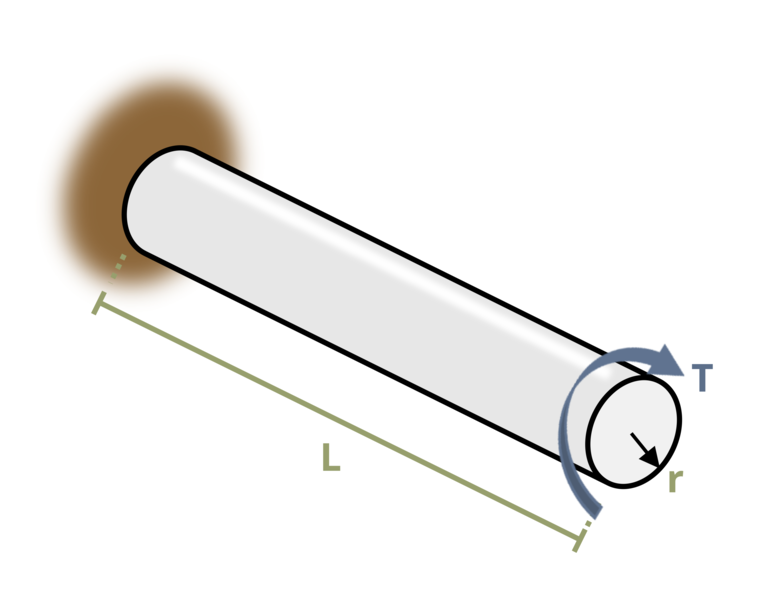
\includegraphics[keepaspectratio]{images/280.png}}
{[}Problem adapted from © Kurt Gramoll CC BY NC-SA 4.0{]}

\begin{Shaded}
\begin{Highlighting}[]
\NormalTok{\#| standalone: true}
\NormalTok{\#| viewerHeight: 600}
\NormalTok{\#| components: [viewer]}

\NormalTok{from shiny import App, render, ui, reactive}
\NormalTok{import random}
\NormalTok{import asyncio}
\NormalTok{import io}
\NormalTok{import math}
\NormalTok{import string}
\NormalTok{from datetime import datetime}
\NormalTok{from pathlib import Path}

\NormalTok{def generate\_random\_letters(length):}
\NormalTok{    \# Generate a random string of letters of specified length}
\NormalTok{    return \textquotesingle{}\textquotesingle{}.join(random.choice(string.ascii\_lowercase) for \_ in range(length))}

\NormalTok{problem\_ID="280"}
\NormalTok{L=reactive.Value("\_\_")}
\NormalTok{angle=reactive.Value("\_\_")}
\NormalTok{tmax=reactive.Value("\_\_")}

\NormalTok{attempts=["Timestamp,Attempt,Answer,Feedback\textbackslash{}n"]}

\NormalTok{app\_ui = ui.page\_fluid(}
\NormalTok{    \#ui.markdown("**Please enter your ID number from your instructor and click to generate your problem**"),}
\NormalTok{    \#ui.input\_text("ID","", placeholder="Enter ID Number Here"),}
\NormalTok{    \#ui.input\_action\_button("generate\_problem", "Generate Problem", class\_="btn{-}primary"),}
\NormalTok{    ui.markdown("**Problem Statement**"),}
\NormalTok{    ui.output\_ui("ui\_problem\_statement"),}
\NormalTok{    ui.input\_text("answer","Your Answer in units of in", placeholder="Please enter your answer"),}
\NormalTok{    ui.input\_action\_button("submit", "Check Answer", class\_="btn{-}primary"),}
\NormalTok{    \#ui.download\_button("download", "Download File to Submit", class\_="btn{-}success"),}
\NormalTok{)}

\NormalTok{def server(input, output, session):}
\NormalTok{    \# Initialize a counter for attempts}
\NormalTok{    attempt\_counter = reactive.Value(0)}

\NormalTok{    @output}
\NormalTok{    @render.ui}
\NormalTok{    def ui\_problem\_statement():}
\NormalTok{        randomize\_vars()}
\NormalTok{        return[ui.markdown(f"When a torque, T, is applied to a rod of length L = \{L()\} ft, it undergoes an angle of twist of \{angle()\}° before it fails due to shear stress. If the maximum shear stress in the bar is τ\textless{}sub\textgreater{}max\textless{}/sub\textgreater{} = \{tmax()\} ksi, determine the diameter of the rod. Assume G = 11,800 ksi.")]}
    
\NormalTok{    \#@reactive.Effect}
\NormalTok{    \#@reactive.event(input.generate\_problem)}
\NormalTok{    def randomize\_vars():}
\NormalTok{        random.seed(101)}
\NormalTok{        L.set(random.randrange(25,100,1)/10)}
\NormalTok{        angle.set(random.randrange(30,50,1))}
\NormalTok{        tmax.set(random.randrange(20,40,1))}
        
\NormalTok{    @reactive.Effect}
\NormalTok{    @reactive.event(input.submit)}
\NormalTok{    def \_():}
\NormalTok{        attempt\_counter.set(attempt\_counter() + 1)  \# Increment the attempt counter on each submission.}
\NormalTok{        r = tmax()*L()*12/(angle()*math.pi/180*11800)}
\NormalTok{        instr = 2*r}
\NormalTok{        if math.isclose(float(input.answer()), instr, rel\_tol=0.01):}
\NormalTok{            check = "*Correct*"}
\NormalTok{            correct\_indicator = "JL"}
\NormalTok{        else:}
\NormalTok{            check = "*Not Correct.*"}
\NormalTok{            correct\_indicator = "JG"}

\NormalTok{        \# Generate random parts for the encoded attempt.}
\NormalTok{        random\_start = generate\_random\_letters(4)}
\NormalTok{        random\_middle = generate\_random\_letters(4)}
\NormalTok{        random\_end = generate\_random\_letters(4)}
\NormalTok{        \#encoded\_attempt = f"\{random\_start\}\{problem\_ID\}{-}\{random\_middle\}\{attempt\_counter()\}\{correct\_indicator\}{-}\{random\_end\}\{input.ID()\}"}

\NormalTok{        \# Store the most recent encoded attempt in a reactive value so it persists across submissions}
\NormalTok{        \#session.encoded\_attempt = reactive.Value(encoded\_attempt)}

\NormalTok{        \# Append the attempt data to the attempts list without the encoded attempt}
\NormalTok{        attempts.append(f"\{datetime.now()\}, \{attempt\_counter()\}, \{input.answer()\}, \{check\}\textbackslash{}n")}

\NormalTok{        \# Show feedback to the user.}
\NormalTok{        feedback = ui.markdown(f"Your answer of \{input.answer()\} is \{check\}.")}
\NormalTok{        m = ui.modal(}
\NormalTok{            feedback,}
\NormalTok{            title="Feedback",}
\NormalTok{            easy\_close=True}
\NormalTok{        )}
\NormalTok{        ui.modal\_show(m)}

\NormalTok{    \#@render.download(filename=lambda: f"Problem\_Log{-}\{problem\_ID\}{-}\{input.ID()\}.csv")}
\NormalTok{    async def download():}
\NormalTok{        \# Start the CSV with the encoded attempt (without label)}
\NormalTok{        final\_encoded = session.encoded\_attempt() if session.encoded\_attempt is not None else "No attempts"}
\NormalTok{        yield f"\{final\_encoded\}\textbackslash{}n\textbackslash{}n"}
        
\NormalTok{        \# Write the header for the remaining CSV data once}
\NormalTok{        yield "Timestamp,Attempt,Answer,Feedback\textbackslash{}n"}
        
\NormalTok{        \# Write the attempts data, ensure that the header from the attempts list is not written again}
\NormalTok{        for attempt in attempts[1:]:  \# Skip the first element which is the header}
\NormalTok{            await asyncio.sleep(0.25)  \# This delay may not be necessary; adjust as needed}
\NormalTok{            yield attempt}

\NormalTok{\# App installation}
\NormalTok{app = App(app\_ui, server)}
\end{Highlighting}
\end{Shaded}

\chapter*{Problem 6.20 - Torsional
Deformation}\label{problem-6.20---torsional-deformation}
\addcontentsline{toc}{chapter}{Problem 6.20 - Torsional Deformation}

\markboth{Problem 6.20 - Torsional Deformation}{Problem 6.20 - Torsional
Deformation}

\pandocbounded{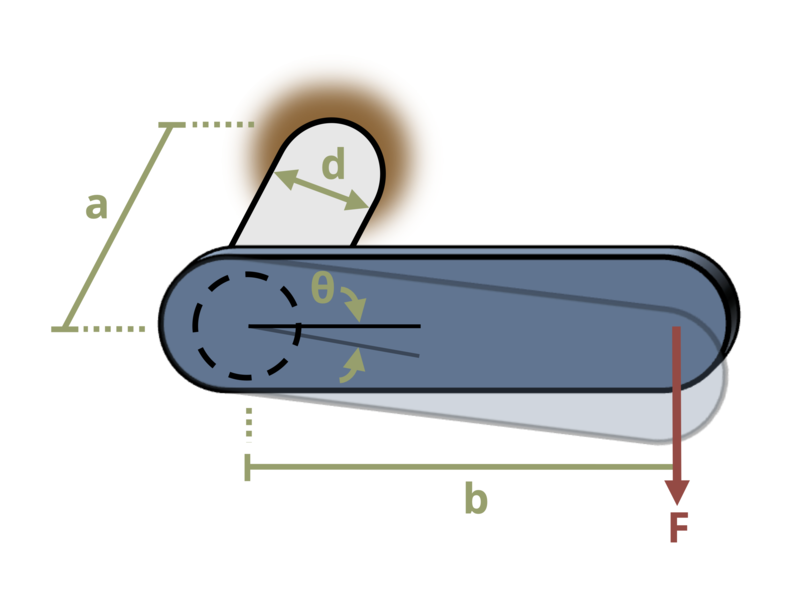
\includegraphics[keepaspectratio]{images/283.png}}
{[}Problem adapted from © Kurt Gramoll CC BY NC-SA 4.0{]}

\begin{Shaded}
\begin{Highlighting}[]
\NormalTok{\#| standalone: true}
\NormalTok{\#| viewerHeight: 600}
\NormalTok{\#| components: [viewer]}

\NormalTok{from shiny import App, render, ui, reactive}
\NormalTok{import random}
\NormalTok{import asyncio}
\NormalTok{import io}
\NormalTok{import math}
\NormalTok{import string}
\NormalTok{from datetime import datetime}
\NormalTok{from pathlib import Path}

\NormalTok{def generate\_random\_letters(length):}
\NormalTok{    \# Generate a random string of letters of specified length}
\NormalTok{    return \textquotesingle{}\textquotesingle{}.join(random.choice(string.ascii\_lowercase) for \_ in range(length))  }

\NormalTok{problem\_ID="283"}
\NormalTok{a=reactive.Value("\_\_")}
\NormalTok{b=reactive.Value("\_\_")}
\NormalTok{d=reactive.Value("\_\_")}
\NormalTok{angle=reactive.Value("\_\_")}
  
\NormalTok{attempts=["Timestamp,Attempt,Answer,Feedback\textbackslash{}n"]}

\NormalTok{app\_ui = ui.page\_fluid(}
\NormalTok{    \#ui.markdown("**Please enter your ID number from your instructor and click to generate your problem**"),}
\NormalTok{    \#ui.input\_text("ID","", placeholder="Enter ID Number Here"),}
\NormalTok{    \#ui.input\_action\_button("generate\_problem", "Generate Problem", class\_="btn{-}primary"),}
\NormalTok{    ui.markdown("**Problem Statement**"),}
\NormalTok{    ui.output\_ui("ui\_problem\_statement"),}
\NormalTok{    ui.input\_text("answer","Your Answer in units of N", placeholder="Please enter your answer"),}
\NormalTok{    ui.input\_action\_button("submit", "Check Answer", class\_="btn{-}primary"),}
\NormalTok{    \#ui.download\_button("download", "Download File to Submit", class\_="btn{-}success"),}
\NormalTok{)}

\NormalTok{def server(input, output, session):}
\NormalTok{    \# Initialize a counter for attempts}
\NormalTok{    attempt\_counter = reactive.Value(0)}

\NormalTok{    @output}
\NormalTok{    @render.ui}
\NormalTok{    def ui\_problem\_statement():}
\NormalTok{        randomize\_vars()}
\NormalTok{        return[ui.markdown(f"A load F is applied to a bracket that is firmly attached a wall as shown. Assume distances a = \{a()\} mm and b = \{b()\} mm, and diameter d = \{d()\} mm. If the bracket rotates through Θ =  \{angle()\}°, determine the load F. Assume E = 200 GPa and ν = 0.29.")]}
    
\NormalTok{    \#@reactive.Effect}
\NormalTok{    \#@reactive.event(input.generate\_problem)}
\NormalTok{    def randomize\_vars():}
\NormalTok{        random.seed(101)}
\NormalTok{        a.set(random.randrange(50,100,1))}
\NormalTok{        b.set(a()+random.randrange(30,60,1))}
\NormalTok{        d.set(random.randrange(15,30,1))}
\NormalTok{        angle.set(random.randrange(10,30,1)/10)}
        
\NormalTok{    @reactive.Effect}
\NormalTok{    @reactive.event(input.submit)}
\NormalTok{    def \_():}
\NormalTok{        attempt\_counter.set(attempt\_counter() + 1)  \# Increment the attempt counter on each submission.}
\NormalTok{        G = 200*10**9/(2*1.29)}
\NormalTok{        J = math.pi/2*(d()/2000)**4}
\NormalTok{        T = angle()*math.pi/180*J*G/(a()/1000)}
\NormalTok{        instr= T/(b()/1000)}
\NormalTok{        if math.isclose(float(input.answer()), instr, rel\_tol=0.01):}
\NormalTok{            check = "*Correct*"}
\NormalTok{            correct\_indicator = "JL"}
\NormalTok{        else:}
\NormalTok{            check = "*Not Correct.*"}
\NormalTok{            correct\_indicator = "JG"}

\NormalTok{        \# Generate random parts for the encoded attempt.}
\NormalTok{        random\_start = generate\_random\_letters(4)}
\NormalTok{        random\_middle = generate\_random\_letters(4)}
\NormalTok{        random\_end = generate\_random\_letters(4)}
\NormalTok{        \#encoded\_attempt = f"\{random\_start\}\{problem\_ID\}{-}\{random\_middle\}\{attempt\_counter()\}\{correct\_indicator\}{-}\{random\_end\}\{input.ID()\}"}

\NormalTok{        \# Store the most recent encoded attempt in a reactive value so it persists across submissions}
\NormalTok{        \#session.encoded\_attempt = reactive.Value(encoded\_attempt)}

\NormalTok{        \# Append the attempt data to the attempts list without the encoded attempt}
\NormalTok{        attempts.append(f"\{datetime.now()\}, \{attempt\_counter()\}, \{input.answer()\}, \{check\}\textbackslash{}n")}

\NormalTok{        \# Show feedback to the user.}
\NormalTok{        feedback = ui.markdown(f"Your answer of \{input.answer()\} is \{check\}.")}
\NormalTok{        m = ui.modal(}
\NormalTok{            feedback,}
\NormalTok{            title="Feedback",}
\NormalTok{            easy\_close=True}
\NormalTok{        )}
\NormalTok{        ui.modal\_show(m)}

\NormalTok{    \#@render.download(filename=lambda: f"Problem\_Log{-}\{problem\_ID\}{-}\{input.ID()\}.csv")}
\NormalTok{    async def download():}
\NormalTok{        \# Start the CSV with the encoded attempt (without label)}
\NormalTok{        final\_encoded = session.encoded\_attempt() if session.encoded\_attempt is not None else "No attempts"}
\NormalTok{        yield f"\{final\_encoded\}\textbackslash{}n\textbackslash{}n"}
        
\NormalTok{        \# Write the header for the remaining CSV data once}
\NormalTok{        yield "Timestamp,Attempt,Answer,Feedback\textbackslash{}n"}
        
\NormalTok{        \# Write the attempts data, ensure that the header from the attempts list is not written again}
\NormalTok{        for attempt in attempts[1:]:  \# Skip the first element which is the header}
\NormalTok{            await asyncio.sleep(0.25)  \# This delay may not be necessary; adjust as needed}
\NormalTok{            yield attempt}
            
\NormalTok{\# App installation}
\NormalTok{app = App(app\_ui, server)}
\end{Highlighting}
\end{Shaded}

\chapter*{Problem 6.21 - Torsional
Deformation}\label{problem-6.21---torsional-deformation}
\addcontentsline{toc}{chapter}{Problem 6.21 - Torsional Deformation}

\markboth{Problem 6.21 - Torsional Deformation}{Problem 6.21 - Torsional
Deformation}

\pandocbounded{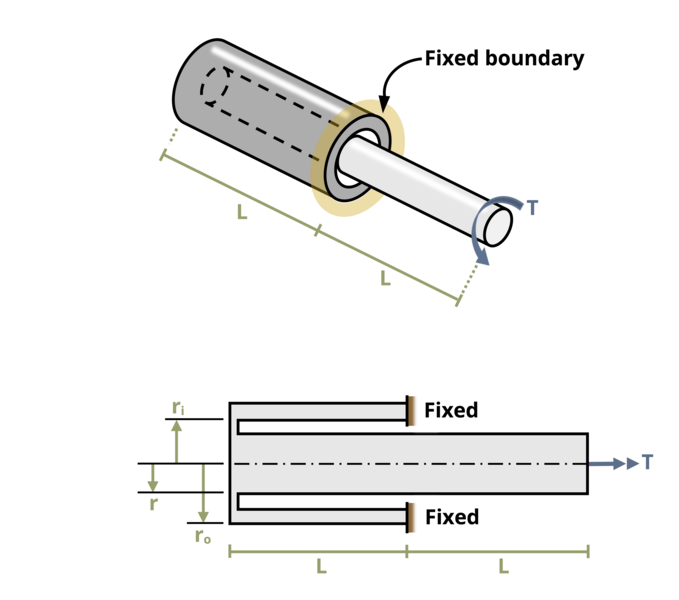
\includegraphics[keepaspectratio]{images/285.png}}
{[}Problem adapted from © Kurt Gramoll CC BY NC-SA 4.0{]}

\begin{Shaded}
\begin{Highlighting}[]
\NormalTok{\#| standalone: true}
\NormalTok{\#| viewerHeight: 600}
\NormalTok{\#| components: [viewer]}

\NormalTok{from shiny import App, render, ui, reactive}
\NormalTok{import random}
\NormalTok{import asyncio}
\NormalTok{import io}
\NormalTok{import math}
\NormalTok{import string}
\NormalTok{from datetime import datetime}
\NormalTok{from pathlib import Path}

\NormalTok{def generate\_random\_letters(length):}
\NormalTok{    \# Generate a random string of letters of specified length}
\NormalTok{    return \textquotesingle{}\textquotesingle{}.join(random.choice(string.ascii\_lowercase) for \_ in range(length))  }

\NormalTok{problem\_ID="285"}
\NormalTok{r=reactive.Value("\_\_")}
\NormalTok{ri=reactive.Value("\_\_")}
\NormalTok{ro=reactive.Value("\_\_")}
\NormalTok{T=reactive.Value("\_\_")}
  
\NormalTok{attempts=["Timestamp,Attempt,Answer,Feedback\textbackslash{}n"]}

\NormalTok{app\_ui = ui.page\_fluid(}
\NormalTok{    \#ui.markdown("**Please enter your ID number from your instructor and click to generate your problem**"),}
\NormalTok{    \#ui.input\_text("ID","", placeholder="Enter ID Number Here"),}
\NormalTok{    \#ui.input\_action\_button("generate\_problem", "Generate Problem", class\_="btn{-}primary"),}
\NormalTok{    ui.markdown("**Problem Statement**"),}
\NormalTok{    ui.output\_ui("ui\_problem\_statement"),}
\NormalTok{    ui.input\_text("answer","Your Answer in units of rad", placeholder="Please enter your answer"),}
\NormalTok{    ui.input\_action\_button("submit", "Check Answer", class\_="btn{-}primary"),}
\NormalTok{    \#ui.download\_button("download", "Download File to Submit", class\_="btn{-}success"),}
\NormalTok{)}

\NormalTok{def server(input, output, session):}
\NormalTok{    \# Initialize a counter for attempts}
\NormalTok{    attempt\_counter = reactive.Value(0)}

\NormalTok{    @output}
\NormalTok{    @render.ui}
\NormalTok{    def ui\_problem\_statement():}
\NormalTok{        randomize\_vars()}
\NormalTok{        return[ui.markdown(f"A solid cylinder of radius r = \{r()\} mm and length L = 5 cm is rigidly attached to a hollow cylinder of inner radius r\textless{}sub\textgreater{}i\textless{}/sub\textgreater{} = \{ri()\} mm and outer radius r\textless{}sub\textgreater{}o\textless{}/sub\textgreater{} = \{ro()\} mm to form a compact torsional spring. A torque T = \{T()\} N{-}m is applied at the free end. Determine the total rotation at the free end. Assume E = 200 GPa and ν = 0.29.")]}
    
\NormalTok{    \#@reactive.Effect}
\NormalTok{    \#@reactive.event(input.generate\_problem)}
\NormalTok{    def randomize\_vars():}
\NormalTok{        random.seed(101)}
\NormalTok{        r.set(random.randrange(10,20,1))}
\NormalTok{        ri.set(r()+random.randrange(3,5,1))}
\NormalTok{        ro.set(ri()+random.randrange(3,5,1))}
\NormalTok{        T.set(random.randrange(500,1000,10))}
        
\NormalTok{    @reactive.Effect}
\NormalTok{    @reactive.event(input.submit)}
\NormalTok{    def \_():}
\NormalTok{        attempt\_counter.set(attempt\_counter() + 1)  \# Increment the attempt counter on each submission.}
\NormalTok{        G = 200*10**9/(2*1.29)}
\NormalTok{        Jab = ((ro()/1000)**4{-}(ri()/1000)**4)*math.pi/2}
\NormalTok{        Jbc = (r()/1000)**4*math.pi/2}
\NormalTok{        instr= T()*0.05/(G*Jab)+T()*0.1/(G*Jbc)}
\NormalTok{        if math.isclose(float(input.answer()), instr, rel\_tol=0.01):}
\NormalTok{            check = "*Correct*"}
\NormalTok{            correct\_indicator = "JL"}
\NormalTok{        else:}
\NormalTok{            check = "*Not Correct.*"}
\NormalTok{            correct\_indicator = "JG"}

\NormalTok{        \# Generate random parts for the encoded attempt.}
\NormalTok{        random\_start = generate\_random\_letters(4)}
\NormalTok{        random\_middle = generate\_random\_letters(4)}
\NormalTok{        random\_end = generate\_random\_letters(4)}
\NormalTok{        \#encoded\_attempt = f"\{random\_start\}\{problem\_ID\}{-}\{random\_middle\}\{attempt\_counter()\}\{correct\_indicator\}{-}\{random\_end\}\{input.ID()\}"}

\NormalTok{        \# Store the most recent encoded attempt in a reactive value so it persists across submissions}
\NormalTok{        \#session.encoded\_attempt = reactive.Value(encoded\_attempt)}

\NormalTok{        \# Append the attempt data to the attempts list without the encoded attempt}
\NormalTok{        attempts.append(f"\{datetime.now()\}, \{attempt\_counter()\}, \{input.answer()\}, \{check\}\textbackslash{}n")}

\NormalTok{        \# Show feedback to the user.}
\NormalTok{        feedback = ui.markdown(f"Your answer of \{input.answer()\} is \{check\}.")}
\NormalTok{        m = ui.modal(}
\NormalTok{            feedback,}
\NormalTok{            title="Feedback",}
\NormalTok{            easy\_close=True}
\NormalTok{        )}
\NormalTok{        ui.modal\_show(m)}

\NormalTok{    \#@render.download(filename=lambda: f"Problem\_Log{-}\{problem\_ID\}{-}\{input.ID()\}.csv")}
\NormalTok{    async def download():}
\NormalTok{        \# Start the CSV with the encoded attempt (without label)}
\NormalTok{        final\_encoded = session.encoded\_attempt() if session.encoded\_attempt is not None else "No attempts"}
\NormalTok{        yield f"\{final\_encoded\}\textbackslash{}n\textbackslash{}n"}
        
\NormalTok{        \# Write the header for the remaining CSV data once}
\NormalTok{        yield "Timestamp,Attempt,Answer,Feedback\textbackslash{}n"}
        
\NormalTok{        \# Write the attempts data, ensure that the header from the attempts list is not written again}
\NormalTok{        for attempt in attempts[1:]:  \# Skip the first element which is the header}
\NormalTok{            await asyncio.sleep(0.25)  \# This delay may not be necessary; adjust as needed}
\NormalTok{            yield attempt}
            
\NormalTok{\# App installation}
\NormalTok{app = App(app\_ui, server)}
\end{Highlighting}
\end{Shaded}

\chapter*{Problem 6.22 - Power Transmission \& Gear
Assemblies}\label{problem-6.22---power-transmission-gear-assemblies}
\addcontentsline{toc}{chapter}{Problem 6.22 - Power Transmission \& Gear
Assemblies}

\markboth{Problem 6.22 - Power Transmission \& Gear Assemblies}{Problem
6.22 - Power Transmission \& Gear Assemblies}

\pandocbounded{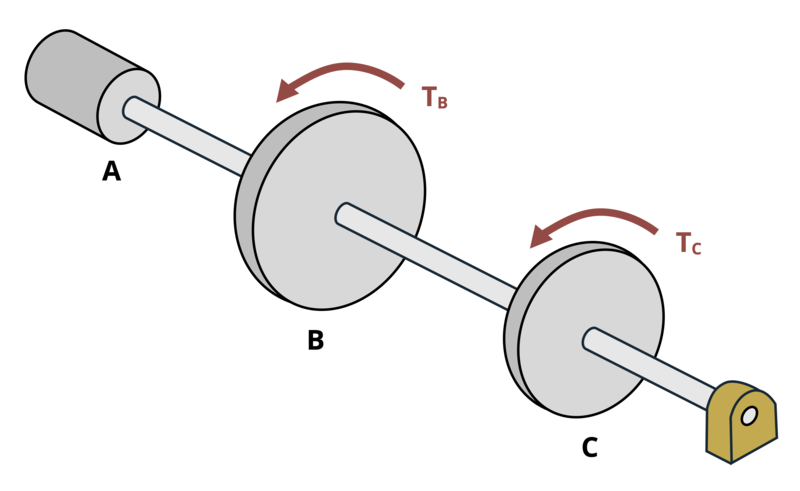
\includegraphics[keepaspectratio]{images/669.png}}
{[}Problem adapted from © Chris Galitz CC BY NC-SA 4.0{]}

\begin{Shaded}
\begin{Highlighting}[]
\NormalTok{\#| standalone: true}
\NormalTok{\#| viewerHeight: 600}
\NormalTok{\#| components: [viewer]}

\NormalTok{from shiny import App, render, ui, reactive}
\NormalTok{import random}
\NormalTok{import asyncio}
\NormalTok{import io}
\NormalTok{import math}
\NormalTok{import string}
\NormalTok{from datetime import datetime}
\NormalTok{from pathlib import Path}

\NormalTok{def generate\_random\_letters(length):}
\NormalTok{    \# Generate a random string of letters of specified length}
\NormalTok{    return \textquotesingle{}\textquotesingle{}.join(random.choice(string.ascii\_lowercase) for \_ in range(length))  }

\NormalTok{problem\_ID="669"}
\NormalTok{P=reactive.Value("\_\_")}
\NormalTok{rpm=reactive.Value("\_\_")}
\NormalTok{T=reactive.Value("\_\_")}

\NormalTok{attempts=["Timestamp,Attempt,Answer,Feedback\textbackslash{}n"]}

\NormalTok{app\_ui = ui.page\_fluid(}
\NormalTok{    \#ui.markdown("**Please enter your ID number from your instructor and click to generate your problem**"),}
\NormalTok{    \#ui.input\_text("ID","", placeholder="Enter ID Number Here"),}
\NormalTok{    \#ui.input\_action\_button("generate\_problem", "Generate Problem", class\_="btn{-}primary"),}
\NormalTok{    ui.markdown("**Problem Statement**"),}
\NormalTok{    ui.output\_ui("ui\_problem\_statement"),}
\NormalTok{    ui.input\_text("answer","Your Answer in units of N*m", placeholder="Please enter your answer"),}
\NormalTok{    ui.input\_action\_button("submit", "Check Answer", class\_="btn{-}primary"),}
\NormalTok{    \#ui.download\_button("download", "Download File to Submit", class\_="btn{-}success"),}
\NormalTok{)}

\NormalTok{def server(input, output, session):}
\NormalTok{    \# Initialize a counter for attempts}
\NormalTok{    attempt\_counter = reactive.Value(0)}

\NormalTok{    @output}
\NormalTok{    @render.ui}
\NormalTok{    def ui\_problem\_statement():}
\NormalTok{        randomize\_vars()}
\NormalTok{        return[ui.markdown(f"The steel shaft is being turned by an electric motor providing \{P()\} kW of power at \{rpm()\} rpm. Power is extracted at B with a torque of \{T()\} N⸱m. Determine the remaining torque available for the gear at C.")]}
    
\NormalTok{    \#@reactive.Effect}
\NormalTok{    \#@reactive.event(input.generate\_problem)}
\NormalTok{    def randomize\_vars():}
\NormalTok{        random.seed(101)}
\NormalTok{        P.set(random.randrange(10, 30, 1))}
\NormalTok{        rpm.set(random.randrange(60, 180, 5))}
\NormalTok{        T.set(random.randrange(200, 400, 10))}
        
\NormalTok{    @reactive.Effect}
\NormalTok{    @reactive.event(input.submit)}
\NormalTok{    def \_():}
\NormalTok{        attempt\_counter.set(attempt\_counter() + 1)  \# Increment the attempt counter on each submission.}
\NormalTok{        TA = P()*1000/(2*math.pi*rpm()/60)}
\NormalTok{        instr= TA{-}T()}
\NormalTok{        if math.isclose(float(input.answer()), instr, rel\_tol=0.01):}
\NormalTok{            check = "*Correct*"}
\NormalTok{            correct\_indicator = "JL"}
\NormalTok{        else:}
\NormalTok{            check = "*Not Correct.*"}
\NormalTok{            correct\_indicator = "JG"}

\NormalTok{        \# Generate random parts for the encoded attempt.}
\NormalTok{        random\_start = generate\_random\_letters(4)}
\NormalTok{        random\_middle = generate\_random\_letters(4)}
\NormalTok{        random\_end = generate\_random\_letters(4)}
\NormalTok{        \#encoded\_attempt = f"\{random\_start\}\{problem\_ID\}{-}\{random\_middle\}\{attempt\_counter()\}\{correct\_indicator\}{-}\{random\_end\}\{input.ID()\}"}

\NormalTok{        \# Store the most recent encoded attempt in a reactive value so it persists across submissions}
\NormalTok{        \#session.encoded\_attempt = reactive.Value(encoded\_attempt)}

\NormalTok{        \# Append the attempt data to the attempts list without the encoded attempt}
\NormalTok{        attempts.append(f"\{datetime.now()\}, \{attempt\_counter()\}, \{input.answer()\}, \{check\}\textbackslash{}n")}

\NormalTok{        \# Show feedback to the user.}
\NormalTok{        feedback = ui.markdown(f"Your answer of \{input.answer()\} is \{check\}.")}
\NormalTok{        m = ui.modal(}
\NormalTok{            feedback,}
\NormalTok{            title="Feedback",}
\NormalTok{            easy\_close=True}
\NormalTok{        )}
\NormalTok{        ui.modal\_show(m)}

\NormalTok{    \#@render.download(filename=lambda: f"Problem\_Log{-}\{problem\_ID\}{-}\{input.ID()\}.csv")}
\NormalTok{    async def download():}
\NormalTok{        \# Start the CSV with the encoded attempt (without label)}
\NormalTok{        final\_encoded = session.encoded\_attempt() if session.encoded\_attempt is not None else "No attempts"}
\NormalTok{        yield f"\{final\_encoded\}\textbackslash{}n\textbackslash{}n"}
        
\NormalTok{        \# Write the header for the remaining CSV data once}
\NormalTok{        yield "Timestamp,Attempt,Answer,Feedback\textbackslash{}n"}
        
\NormalTok{        \# Write the attempts data, ensure that the header from the attempts list is not written again}
\NormalTok{        for attempt in attempts[1:]:  \# Skip the first element which is the header}
\NormalTok{            await asyncio.sleep(0.25)  \# This delay may not be necessary; adjust as needed}
\NormalTok{            yield attempt}

\NormalTok{\# App installation}
\NormalTok{app = App(app\_ui, server)}
\end{Highlighting}
\end{Shaded}

\chapter*{Problem 6.23 - Power Transmission \& Gear
Assemblies}\label{problem-6.23---power-transmission-gear-assemblies}
\addcontentsline{toc}{chapter}{Problem 6.23 - Power Transmission \& Gear
Assemblies}

\markboth{Problem 6.23 - Power Transmission \& Gear Assemblies}{Problem
6.23 - Power Transmission \& Gear Assemblies}

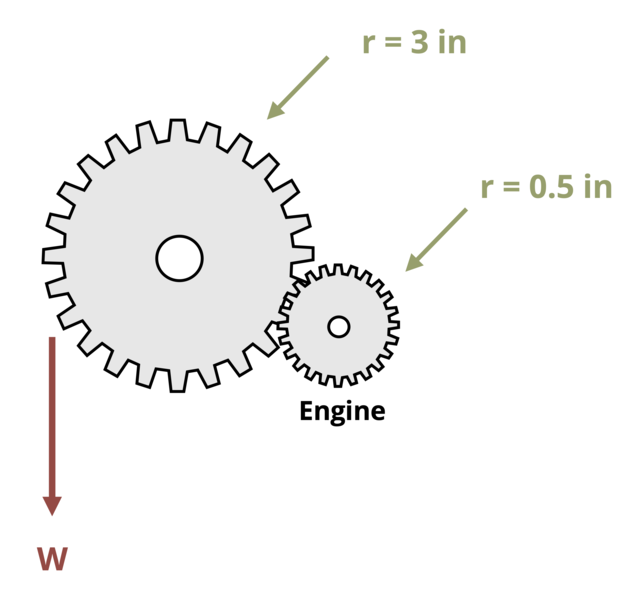
\includegraphics[width=3.125in,height=\textheight,keepaspectratio]{images/670.png}
{[}Problem adapted from © Chris Galitz CC BY NC-SA 4.0{]}

\begin{Shaded}
\begin{Highlighting}[]
\NormalTok{\#| standalone: true}
\NormalTok{\#| viewerHeight: 600}
\NormalTok{\#| components: [viewer]}

\NormalTok{from shiny import App, render, ui, reactive}
\NormalTok{import random}
\NormalTok{import asyncio}
\NormalTok{import io}
\NormalTok{import math}
\NormalTok{import string}
\NormalTok{from datetime import datetime}
\NormalTok{from pathlib import Path}

\NormalTok{def generate\_random\_letters(length):}
\NormalTok{    \# Generate a random string of letters of specified length}
\NormalTok{    return \textquotesingle{}\textquotesingle{}.join(random.choice(string.ascii\_lowercase) for \_ in range(length))  }

\NormalTok{problem\_ID="670"}
\NormalTok{hp=reactive.Value("\_\_")}
\NormalTok{rpm=reactive.Value("\_\_")}

\NormalTok{attempts=["Timestamp,Attempt,Answer,Feedback\textbackslash{}n"]}

\NormalTok{app\_ui = ui.page\_fluid(}
\NormalTok{    \#ui.markdown("**Please enter your ID number from your instructor and click to generate your problem**"),}
\NormalTok{    \#ui.input\_text("ID","", placeholder="Enter ID Number Here"),}
\NormalTok{    \#ui.input\_action\_button("generate\_problem", "Generate Problem", class\_="btn{-}primary"),}
\NormalTok{    ui.markdown("**Problem Statement**"),}
\NormalTok{    ui.output\_ui("ui\_problem\_statement"),}
\NormalTok{    ui.input\_text("answer","Your Answer in units of lb", placeholder="Please enter your answer"),}
\NormalTok{    ui.input\_action\_button("submit", "Check Answer", class\_="btn{-}primary"),}
\NormalTok{    \#ui.download\_button("download", "Download File to Submit", class\_="btn{-}success"),}
\NormalTok{)}

\NormalTok{def server(input, output, session):}
\NormalTok{    \# Initialize a counter for attempts}
\NormalTok{    attempt\_counter = reactive.Value(0)}

\NormalTok{    @output}
\NormalTok{    @render.ui}
\NormalTok{    def ui\_problem\_statement():}
\NormalTok{        randomize\_vars()}
\NormalTok{        return[ui.markdown(f"A lawnmower engine supplying \{hp()\} hp running at \{rpm()\} rpm is being used to power a homemade winch. Given the gearing shown, determine the heaviest load that can be lifted.")]}
    
\NormalTok{    \#@reactive.Effect}
\NormalTok{    \#@reactive.event(input.generate\_problem)}
\NormalTok{    def randomize\_vars():}
\NormalTok{        random.seed(101)}
\NormalTok{        hp.set(random.randrange(10, 50, 1)/10)}
\NormalTok{        rpm.set(random.randrange(2000, 4000, 100))}
        
\NormalTok{    @reactive.Effect}
\NormalTok{    @reactive.event(input.submit)}
\NormalTok{    def \_():}
\NormalTok{        attempt\_counter.set(attempt\_counter() + 1)  \# Increment the attempt counter on each submission.}
\NormalTok{        T = hp()*550/(2*math.pi*rpm()/60)*12}
\NormalTok{        instr= T/0.5}
\NormalTok{        if math.isclose(float(input.answer()), instr, rel\_tol=0.01):}
\NormalTok{            check = "*Correct*"}
\NormalTok{            correct\_indicator = "JL"}
\NormalTok{        else:}
\NormalTok{            check = "*Not Correct.*"}
\NormalTok{            correct\_indicator = "JG"}

\NormalTok{        \# Generate random parts for the encoded attempt.}
\NormalTok{        random\_start = generate\_random\_letters(4)}
\NormalTok{        random\_middle = generate\_random\_letters(4)}
\NormalTok{        random\_end = generate\_random\_letters(4)}
\NormalTok{        \#encoded\_attempt = f"\{random\_start\}\{problem\_ID\}{-}\{random\_middle\}\{attempt\_counter()\}\{correct\_indicator\}{-}\{random\_end\}\{input.ID()\}"}

\NormalTok{        \# Store the most recent encoded attempt in a reactive value so it persists across submissions}
\NormalTok{        \#session.encoded\_attempt = reactive.Value(encoded\_attempt)}

\NormalTok{        \# Append the attempt data to the attempts list without the encoded attempt}
\NormalTok{        attempts.append(f"\{datetime.now()\}, \{attempt\_counter()\}, \{input.answer()\}, \{check\}\textbackslash{}n")}

\NormalTok{        \# Show feedback to the user.}
\NormalTok{        feedback = ui.markdown(f"Your answer of \{input.answer()\} is \{check\}.")}
\NormalTok{        m = ui.modal(}
\NormalTok{            feedback,}
\NormalTok{            title="Feedback",}
\NormalTok{            easy\_close=True}
\NormalTok{        )}
\NormalTok{        ui.modal\_show(m)}

\NormalTok{    \#@render.download(filename=lambda: f"Problem\_Log{-}\{problem\_ID\}{-}\{input.ID()\}.csv")}
\NormalTok{    async def download():}
\NormalTok{        \# Start the CSV with the encoded attempt (without label)}
\NormalTok{        final\_encoded = session.encoded\_attempt() if session.encoded\_attempt is not None else "No attempts"}
\NormalTok{        yield f"\{final\_encoded\}\textbackslash{}n\textbackslash{}n"}
        
\NormalTok{        \# Write the header for the remaining CSV data once}
\NormalTok{        yield "Timestamp,Attempt,Answer,Feedback\textbackslash{}n"}
        
\NormalTok{        \# Write the attempts data, ensure that the header from the attempts list is not written again}
\NormalTok{        for attempt in attempts[1:]:  \# Skip the first element which is the header}
\NormalTok{            await asyncio.sleep(0.25)  \# This delay may not be necessary; adjust as needed}
\NormalTok{            yield attempt}

\NormalTok{\# App installation}
\NormalTok{app = App(app\_ui, server)}
\end{Highlighting}
\end{Shaded}

\chapter*{Problem 6.24 - Power Transmission and Gear
Assemblies}\label{problem-6.24---power-transmission-and-gear-assemblies}
\addcontentsline{toc}{chapter}{Problem 6.24 - Power Transmission and
Gear Assemblies}

\markboth{Problem 6.24 - Power Transmission and Gear Assemblies}{Problem
6.24 - Power Transmission and Gear Assemblies}

{[}Problem adapted from © Chris Galitz CC BY NC-SA 4.0{]}

\begin{Shaded}
\begin{Highlighting}[]
\NormalTok{\#| standalone: true}
\NormalTok{\#| viewerHeight: 600}
\NormalTok{\#| components: [viewer]}

\NormalTok{from shiny import App, render, ui, reactive}
\NormalTok{import random}
\NormalTok{import asyncio}
\NormalTok{import io}
\NormalTok{import math}
\NormalTok{import string}
\NormalTok{from datetime import datetime}
\NormalTok{from pathlib import Path}

\NormalTok{def generate\_random\_letters(length):}
\NormalTok{    \# Generate a random string of letters of specified length}
\NormalTok{    return \textquotesingle{}\textquotesingle{}.join(random.choice(string.ascii\_lowercase) for \_ in range(length))  }

\NormalTok{problem\_ID="671"}
\NormalTok{hp=reactive.Value("\_\_")}
\NormalTok{r=reactive.Value("\_\_")}
\NormalTok{W=reactive.Value("\_\_")}

\NormalTok{attempts=["Timestamp,Attempt,Answer,Feedback\textbackslash{}n"]}

\NormalTok{app\_ui = ui.page\_fluid(}
\NormalTok{    \#ui.markdown("**Please enter your ID number from your instructor and click to generate your problem**"),}
\NormalTok{    \#ui.input\_text("ID","", placeholder="Enter ID Number Here"),}
\NormalTok{    \#ui.input\_action\_button("generate\_problem", "Generate Problem", class\_="btn{-}primary"),}
\NormalTok{    ui.markdown("**Problem Statement**"),}
\NormalTok{    ui.output\_ui("ui\_problem\_statement"),}
\NormalTok{    ui.input\_text("answer","Your Answer in units of rpm", placeholder="Please enter your answer"),}
\NormalTok{    ui.input\_action\_button("submit", "Check Answer", class\_="btn{-}primary"),}
\NormalTok{    \#ui.download\_button("download", "Download File to Submit", class\_="btn{-}success"),}
\NormalTok{)}

\NormalTok{def server(input, output, session):}
\NormalTok{    \# Initialize a counter for attempts}
\NormalTok{    attempt\_counter = reactive.Value(0)}

\NormalTok{    @output}
\NormalTok{    @render.ui}
\NormalTok{    def ui\_problem\_statement():}
\NormalTok{        randomize\_vars()}
\NormalTok{        return[ui.markdown(f"A driver is attempting a burnout in a car with a \{hp()\}{-}hp engine and positraction (both rear wheels receive equal torque). If the tires have radius r = \{r()\} in., support a weight W = \{W()\} lb each, and have a static coefficient of friction of 0.85 with the pavement, determine the rpm of the engine when the tires slip and the burnout starts.")]}
    
\NormalTok{    \#@reactive.Effect}
\NormalTok{    \#@reactive.event(input.generate\_problem)}
\NormalTok{    def randomize\_vars():}
\NormalTok{        random.seed(101)}
\NormalTok{        hp.set(random.randrange(180,250,5))}
\NormalTok{        r.set(random.randrange(130,200,5)/10)}
\NormalTok{        W.set(random.randrange(600,1000,10))}
        
\NormalTok{    @reactive.Effect}
\NormalTok{    @reactive.event(input.submit)}
\NormalTok{    def \_():}
\NormalTok{        attempt\_counter.set(attempt\_counter() + 1)  \# Increment the attempt counter on each submission.}
\NormalTok{        F=0.85*W()}
\NormalTok{        T=F*r()}
\NormalTok{        Ttot=T*2/12}
\NormalTok{        omega=hp()*550/Ttot}
\NormalTok{        instr=60*omega/(2*math.pi)}
\NormalTok{        if math.isclose(float(input.answer()), instr, rel\_tol=0.01):}
\NormalTok{            check = "*Correct*"}
\NormalTok{            correct\_indicator = "JL"}
\NormalTok{        else:}
\NormalTok{            check = "*Not Correct.*"}
\NormalTok{            correct\_indicator = "JG"}

\NormalTok{        \# Generate random parts for the encoded attempt.}
\NormalTok{        random\_start = generate\_random\_letters(4)}
\NormalTok{        random\_middle = generate\_random\_letters(4)}
\NormalTok{        random\_end = generate\_random\_letters(4)}
\NormalTok{        \#encoded\_attempt = f"\{random\_start\}\{problem\_ID\}{-}\{random\_middle\}\{attempt\_counter()\}\{correct\_indicator\}{-}\{random\_end\}\{input.ID()\}"}

\NormalTok{        \# Store the most recent encoded attempt in a reactive value so it persists across submissions}
\NormalTok{        \#session.encoded\_attempt = reactive.Value(encoded\_attempt)}

\NormalTok{        \# Append the attempt data to the attempts list without the encoded attempt}
\NormalTok{        attempts.append(f"\{datetime.now()\}, \{attempt\_counter()\}, \{input.answer()\}, \{check\}\textbackslash{}n")}

\NormalTok{        \# Show feedback to the user.}
\NormalTok{        feedback = ui.markdown(f"Your answer of \{input.answer()\} is \{check\}.")}
\NormalTok{        m = ui.modal(}
\NormalTok{            feedback,}
\NormalTok{            title="Feedback",}
\NormalTok{            easy\_close=True}
\NormalTok{        )}
\NormalTok{        ui.modal\_show(m)}

\NormalTok{    \#@render.download(filename=lambda: f"Problem\_Log{-}\{problem\_ID\}{-}\{input.ID()\}.csv")}
\NormalTok{    async def download():}
\NormalTok{        \# Start the CSV with the encoded attempt (without label)}
\NormalTok{        final\_encoded = session.encoded\_attempt() if session.encoded\_attempt is not None else "No attempts"}
\NormalTok{        yield f"\{final\_encoded\}\textbackslash{}n\textbackslash{}n"}
        
\NormalTok{        \# Write the header for the remaining CSV data once}
\NormalTok{        yield "Timestamp,Attempt,Answer,Feedback\textbackslash{}n"}
        
\NormalTok{        \# Write the attempts data, ensure that the header from the attempts list is not written again}
\NormalTok{        for attempt in attempts[1:]:  \# Skip the first element which is the header}
\NormalTok{            await asyncio.sleep(0.25)  \# This delay may not be necessary; adjust as needed}
\NormalTok{            yield attempt}

\NormalTok{\# App installation}
\NormalTok{app = App(app\_ui, server)}
\end{Highlighting}
\end{Shaded}

\chapter*{Problem 6.26 - Torsional
Stress}\label{problem-6.26---torsional-stress}
\addcontentsline{toc}{chapter}{Problem 6.26 - Torsional Stress}

\markboth{Problem 6.26 - Torsional Stress}{Problem 6.26 - Torsional
Stress}

\pandocbounded{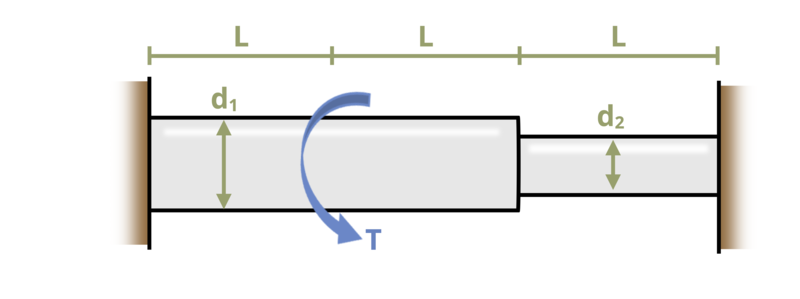
\includegraphics[keepaspectratio]{images/303.png}}
{[}Problem adapted from © Kurt Gramoll CC BY NC-SA 4.0{]}

\begin{Shaded}
\begin{Highlighting}[]
\NormalTok{\#| standalone: true}
\NormalTok{\#| viewerHeight: 600}
\NormalTok{\#| components: [viewer]}

\NormalTok{from shiny import App, render, ui, reactive}
\NormalTok{import random}
\NormalTok{import asyncio}
\NormalTok{import io}
\NormalTok{import math}
\NormalTok{import string}
\NormalTok{from datetime import datetime}
\NormalTok{from pathlib import Path}

\NormalTok{def generate\_random\_letters(length):}
\NormalTok{    \# Generate a random string of letters of specified length}
\NormalTok{    return \textquotesingle{}\textquotesingle{}.join(random.choice(string.ascii\_lowercase) for \_ in range(length))  }

\NormalTok{problem\_ID="303"}
\NormalTok{T=reactive.Value("\_\_")}
\NormalTok{d2=reactive.Value("\_\_")}
\NormalTok{d1=reactive.Value("\_\_")}
\NormalTok{L=reactive.Value("\_\_")}
  
\NormalTok{attempts=["Timestamp,Attempt,Answer,Feedback\textbackslash{}n"]}

\NormalTok{app\_ui = ui.page\_fluid(}
\NormalTok{    \#ui.markdown("**Please enter your ID number from your instructor and click to generate your problem**"),}
\NormalTok{    \#ui.input\_text("ID","", placeholder="Enter ID Number Here"),}
\NormalTok{    \#ui.input\_action\_button("generate\_problem", "Generate Problem", class\_="btn{-}primary"),}
\NormalTok{    ui.markdown("**Problem Statement**"),}
\NormalTok{    ui.output\_ui("ui\_problem\_statement"),}
\NormalTok{    ui.input\_text("answer","Your Answer in units of kN{-}m", placeholder="Please enter your answer"),}
\NormalTok{    ui.input\_action\_button("submit", "Check Answer", class\_="btn{-}primary"),}
\NormalTok{    \#ui.download\_button("download", "Download File to Submit", class\_="btn{-}success"),}
\NormalTok{)}

\NormalTok{def server(input, output, session):}
\NormalTok{    \# Initialize a counter for attempts}
\NormalTok{    attempt\_counter = reactive.Value(0)}

\NormalTok{    @output}
\NormalTok{    @render.ui}
\NormalTok{    def ui\_problem\_statement():}
\NormalTok{        randomize\_vars()}
\NormalTok{        return[ui.markdown(f"Two circular steel rods are firmly welded together and attached between two walls. A torque T = \{T()\} kN{-}m is applied as shown. If diameters d\textless{}sub\textgreater{}1\textless{}/sub\textgreater{} = \{d1()\} mm, d\textless{}sub\textgreater{}2\textless{}/sub\textgreater{} = \{d2()\} mm, and lengths L = \{L()\} m, determine the reaction at the right wall.")]}
    
\NormalTok{    \#@reactive.Effect}
\NormalTok{    \#@reactive.event(input.generate\_problem)}
\NormalTok{    def randomize\_vars():}
\NormalTok{        random.seed(101)}
\NormalTok{        T.set(random.randrange(1,200,1))}
\NormalTok{        d2.set(random.randrange(15,75,1))}
\NormalTok{        d1.set(d2()+random.randrange(10,20,1))}
\NormalTok{        L.set(random.randrange(10,100,1)/10)}

\NormalTok{    @reactive.Effect}
\NormalTok{    @reactive.event(input.submit)}
\NormalTok{    def \_():}
\NormalTok{        attempt\_counter.set(attempt\_counter() + 1)  \# Increment the attempt counter on each submission.}
\NormalTok{        JAB = math.pi*(d1()/2000)**4/2}
\NormalTok{        JBC=JAB}
\NormalTok{        JCD = math.pi*(d2()/2000)**4/2}
\NormalTok{        instr = (T()/JBC+T()/JCD)/(1/JAB+1/JBC+1/JCD)}
\NormalTok{        if math.isclose(float(input.answer()), instr, rel\_tol=0.01):}
\NormalTok{            check = "*Correct*"}
\NormalTok{            correct\_indicator = "JL"}
\NormalTok{        else:}
\NormalTok{            check = "*Not Correct.*"}
\NormalTok{            correct\_indicator = "JG"}

\NormalTok{        \# Generate random parts for the encoded attempt.}
\NormalTok{        random\_start = generate\_random\_letters(4)}
\NormalTok{        random\_middle = generate\_random\_letters(4)}
\NormalTok{        random\_end = generate\_random\_letters(4)}
\NormalTok{        \#encoded\_attempt = f"\{random\_start\}\{problem\_ID\}{-}\{random\_middle\}\{attempt\_counter()\}\{correct\_indicator\}{-}\{random\_end\}\{input.ID()\}"}

\NormalTok{        \# Store the most recent encoded attempt in a reactive value so it persists across submissions}
\NormalTok{        \#session.encoded\_attempt = reactive.Value(encoded\_attempt)}

\NormalTok{        \# Append the attempt data to the attempts list without the encoded attempt}
\NormalTok{        attempts.append(f"\{datetime.now()\}, \{attempt\_counter()\}, \{input.answer()\}, \{check\}\textbackslash{}n")}

\NormalTok{        \# Show feedback to the user.}
\NormalTok{        feedback = ui.markdown(f"Your answer of \{input.answer()\} is \{check\}.")}
\NormalTok{        m = ui.modal(}
\NormalTok{            feedback,}
\NormalTok{            title="Feedback",}
\NormalTok{            easy\_close=True}
\NormalTok{        )}
\NormalTok{        ui.modal\_show(m)}

\NormalTok{    \#@render.download(filename=lambda: f"Problem\_Log{-}\{problem\_ID\}{-}\{input.ID()\}.csv")}
\NormalTok{    async def download():}
\NormalTok{        \# Start the CSV with the encoded attempt (without label)}
\NormalTok{        final\_encoded = session.encoded\_attempt() if session.encoded\_attempt is not None else "No attempts"}
\NormalTok{        yield f"\{final\_encoded\}\textbackslash{}n\textbackslash{}n"}
        
\NormalTok{        \# Write the header for the remaining CSV data once}
\NormalTok{        yield "Timestamp,Attempt,Answer,Feedback\textbackslash{}n"}
        
\NormalTok{        \# Write the attempts data, ensure that the header from the attempts list is not written again}
\NormalTok{        for attempt in attempts[1:]:  \# Skip the first element which is the header}
\NormalTok{            await asyncio.sleep(0.25)  \# This delay may not be necessary; adjust as needed}
\NormalTok{            yield attempt}

\NormalTok{\# App installation}
\NormalTok{app = App(app\_ui, server)}
\end{Highlighting}
\end{Shaded}

\chapter*{Problem 6.27 - Statically Indeterminate
Torsion}\label{problem-6.27---statically-indeterminate-torsion}
\addcontentsline{toc}{chapter}{Problem 6.27 - Statically Indeterminate
Torsion}

\markboth{Problem 6.27 - Statically Indeterminate Torsion}{Problem 6.27
- Statically Indeterminate Torsion}

\pandocbounded{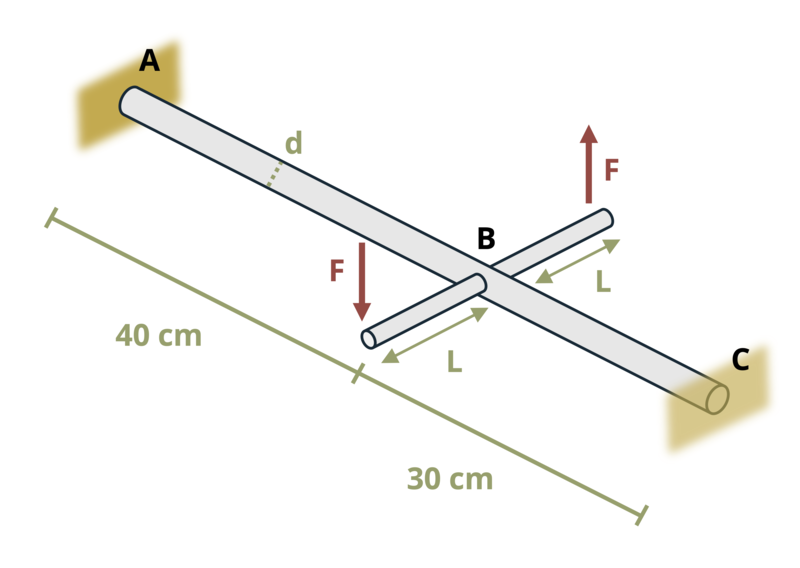
\includegraphics[keepaspectratio]{images/287.png}}
{[}Problem adapted from © Kurt Gramoll CC BY NC-SA 4.0{]}

\begin{Shaded}
\begin{Highlighting}[]
\NormalTok{\#| standalone: true}
\NormalTok{\#| viewerHeight: 600}
\NormalTok{\#| components: [viewer]}

\NormalTok{from shiny import App, render, ui, reactive}
\NormalTok{import random}
\NormalTok{import asyncio}
\NormalTok{import io}
\NormalTok{import math}
\NormalTok{import string}
\NormalTok{from datetime import datetime}
\NormalTok{from pathlib import Path}

\NormalTok{def generate\_random\_letters(length):}
\NormalTok{    \# Generate a random string of letters of specified length}
\NormalTok{    return \textquotesingle{}\textquotesingle{}.join(random.choice(string.ascii\_lowercase) for \_ in range(length)) }

\NormalTok{problem\_ID="287"}
\NormalTok{L=reactive.Value("\_\_")}
\NormalTok{F=reactive.Value("\_\_")}
\NormalTok{d=reactive.Value("\_\_")}
\NormalTok{G = 75}

\NormalTok{attempts=["Timestamp,Attempt,Answer,Feedback\textbackslash{}n"]}

\NormalTok{app\_ui = ui.page\_fluid(}
\NormalTok{    \#ui.markdown("**Please enter your ID number from your instructor and click to generate your problem**"),}
\NormalTok{    \#ui.input\_text("ID","", placeholder="Enter ID Number Here"),}
\NormalTok{    \#ui.input\_action\_button("generate\_problem", "Generate Problem", class\_="btn{-}primary"),}
\NormalTok{    ui.markdown("**Problem Statement**"),}
\NormalTok{    ui.output\_ui("ui\_problem\_statement"),}
\NormalTok{    ui.input\_text("answer","Your Answer in units of MPa", placeholder="Please enter your answer"),}
\NormalTok{    ui.input\_action\_button("submit", "Check Answer", class\_="btn{-}primary"),}
\NormalTok{    \#ui.download\_button("download", "Download File to Submit", class\_="btn{-}success"),}
\NormalTok{)}


\NormalTok{def server(input, output, session):}
\NormalTok{    \# Initialize a counter for attempts}
\NormalTok{    attempt\_counter = reactive.Value(0)}

\NormalTok{    @output}
\NormalTok{    @render.ui}
\NormalTok{    def ui\_problem\_statement():}
\NormalTok{        randomize\_vars()}
\NormalTok{        return[ui.markdown(f"A steel rod of diameter d = \{d()\} mm is attached to walls A and C as shown. Two forces F = \{F()\} kN are applied at distance L = \{L()\} mm. If the shear modulus of the rod G = 75 GPa, determine the maximum shear stress in the rod.")]}
    
\NormalTok{    \#@reactive.Effect}
\NormalTok{    \#@reactive.event(input.generate\_problem)}
\NormalTok{    def randomize\_vars():}
\NormalTok{        random.seed(101)}
\NormalTok{        d.set(random.randrange(20, 60, 1))}
\NormalTok{        F.set(random.randrange(2, 20, 1))}
\NormalTok{        L.set(random.randrange(80, 120, 1))}
        
        
\NormalTok{    @reactive.Effect}
\NormalTok{    @reactive.event(input.submit)}
\NormalTok{    def \_():}
\NormalTok{        attempt\_counter.set(attempt\_counter() + 1)  \# Increment the attempt counter on each submission.}
\NormalTok{        TB = 2*F()*L()}
\NormalTok{        J = (math.pi/2)*(d()/2000)**4}
\NormalTok{        TA = 0.3/0.7*TB}
\NormalTok{        TC = TB{-}TA}
\NormalTok{        instr= ((TC*(d()/2000))/J)/10**6}
\NormalTok{        if math.isclose(float(input.answer()), instr, rel\_tol=0.01):}
\NormalTok{            check = "*Correct*"}
\NormalTok{            correct\_indicator = "JL"}
\NormalTok{        else:}
\NormalTok{            check = "*Not Correct.*"}
\NormalTok{            correct\_indicator = "JG"}

\NormalTok{        \# Generate random parts for the encoded attempt.}
\NormalTok{        random\_start = generate\_random\_letters(4)}
\NormalTok{        random\_middle = generate\_random\_letters(4)}
\NormalTok{        random\_end = generate\_random\_letters(4)}
\NormalTok{        \#encoded\_attempt = f"\{random\_start\}\{problem\_ID\}{-}\{random\_middle\}\{attempt\_counter()\}\{correct\_indicator\}{-}\{random\_end\}\{input.ID()\}"}

\NormalTok{        \# Store the most recent encoded attempt in a reactive value so it persists across submissions}
\NormalTok{        \#session.encoded\_attempt = reactive.Value(encoded\_attempt)}

\NormalTok{        \# Append the attempt data to the attempts list without the encoded attempt}
\NormalTok{        attempts.append(f"\{datetime.now()\}, \{attempt\_counter()\}, \{input.answer()\}, \{check\}\textbackslash{}n")}

\NormalTok{        \# Show feedback to the user.}
\NormalTok{        feedback = ui.markdown(f"Your answer of \{input.answer()\} is \{check\}.")}
\NormalTok{        m = ui.modal(}
\NormalTok{            feedback,}
\NormalTok{            title="Feedback",}
\NormalTok{            easy\_close=True}
\NormalTok{        )}
\NormalTok{        ui.modal\_show(m)}

\NormalTok{    \#@render.download(filename=lambda: f"Problem\_Log{-}\{problem\_ID\}{-}\{input.ID()\}.csv")}
\NormalTok{    async def download():}
\NormalTok{        \# Start the CSV with the encoded attempt (without label)}
\NormalTok{        final\_encoded = session.encoded\_attempt() if session.encoded\_attempt is not None else "No attempts"}
\NormalTok{        yield f"\{final\_encoded\}\textbackslash{}n\textbackslash{}n"}
        
\NormalTok{        \# Write the header for the remaining CSV data once}
\NormalTok{        yield "Timestamp,Attempt,Answer,Feedback\textbackslash{}n"}
        
\NormalTok{        \# Write the attempts data, ensure that the header from the attempts list is not written again}
\NormalTok{        for attempt in attempts[1:]:  \# Skip the first element which is the header}
\NormalTok{            await asyncio.sleep(0.25)  \# This delay may not be necessary; adjust as needed}
\NormalTok{            yield attempt}


\NormalTok{\# App installation}
\NormalTok{app = App(app\_ui, server)}
\end{Highlighting}
\end{Shaded}

\chapter*{Problem 6.28 - Statically Indeterminate
Torsion}\label{problem-6.28---statically-indeterminate-torsion}
\addcontentsline{toc}{chapter}{Problem 6.28 - Statically Indeterminate
Torsion}

\markboth{Problem 6.28 - Statically Indeterminate Torsion}{Problem 6.28
- Statically Indeterminate Torsion}

\pandocbounded{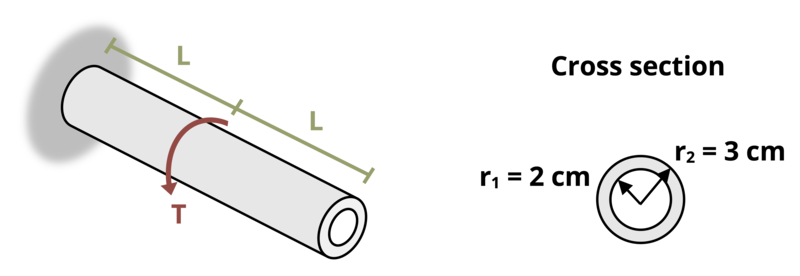
\includegraphics[keepaspectratio]{images/288.png}}
{[}Problem adapted from © Kurt Gramoll CC BY NC-SA 4.0{]}

\begin{Shaded}
\begin{Highlighting}[]
\NormalTok{\#| standalone: true}
\NormalTok{\#| viewerHeight: 600}
\NormalTok{\#| components: [viewer]}

\NormalTok{from shiny import App, render, ui, reactive}
\NormalTok{import random}
\NormalTok{import asyncio}
\NormalTok{import io}
\NormalTok{import math}
\NormalTok{import string}
\NormalTok{from datetime import datetime}
\NormalTok{from pathlib import Path}

\NormalTok{def generate\_random\_letters(length):}
\NormalTok{    \# Generate a random string of letters of specified length}
\NormalTok{    return \textquotesingle{}\textquotesingle{}.join(random.choice(string.ascii\_lowercase) for \_ in range(length)) }

\NormalTok{problem\_ID="288"}
\NormalTok{T=reactive.Value("\_\_")}
\NormalTok{L=reactive.Value("\_\_")}
\NormalTok{G1=reactive.Value("\_\_")}
\NormalTok{G2=reactive.Value("\_\_")}

\NormalTok{attempts=["Timestamp,Attempt,Answer,Feedback\textbackslash{}n"]}

\NormalTok{app\_ui = ui.page\_fluid(}
\NormalTok{    \#ui.markdown("**Please enter your ID number from your instructor and click to generate your problem**"),}
\NormalTok{    \#ui.input\_text("ID","", placeholder="Enter ID Number Here"),}
\NormalTok{    \#ui.input\_action\_button("generate\_problem", "Generate Problem", class\_="btn{-}primary"),}
\NormalTok{    ui.markdown("**Problem Statement**"),}
\NormalTok{    ui.output\_ui("ui\_problem\_statement"),}
\NormalTok{    ui.input\_text("answer","Your Answer in units of MPa", placeholder="Please enter your answer"),}
\NormalTok{    ui.input\_action\_button("submit", "Check Answer", class\_="btn{-}primary"),}
\NormalTok{    \#ui.download\_button("download", "Download File to Submit", class\_="btn{-}success"),}
\NormalTok{)}

\NormalTok{def server(input, output, session):}
\NormalTok{    \# Initialize a counter for attempts}
\NormalTok{    attempt\_counter = reactive.Value(0)}

\NormalTok{    @output}
\NormalTok{    @render.ui}
\NormalTok{    def ui\_problem\_statement():}
\NormalTok{        randomize\_vars()}
\NormalTok{        return[ui.markdown(f"A composite circular rod is made from two different plastics. A torque of T = \{T()\} kN{-}m is applied at the midpoint. The right end is free. What is the maximum stress in either material? Assume length L = \{L()\} cm and the shear modulus of the two materials are G\textless{}sub\textgreater{}1\textless{}/sub\textgreater{} = \{G1()\} GPa and G\textless{}sub\textgreater{}2\textless{}/sub\textgreater{} = \{G2()\} GPa.")]}
    
\NormalTok{    \#@reactive.Effect}
\NormalTok{    \#@reactive.event(input.generate\_problem)}
\NormalTok{    def randomize\_vars():}
\NormalTok{        random.seed(101)}
\NormalTok{        T.set(random.randrange(10, 200, 1)/10)}
\NormalTok{        L.set(random.randrange(10, 50, 1))}
\NormalTok{        G1.set(random.randrange(20, 50, 2)/10)}
\NormalTok{        G2.set(G1()/2)}
        
        
\NormalTok{    @reactive.Effect}
\NormalTok{    @reactive.event(input.submit)}
\NormalTok{    def \_():}
\NormalTok{        attempt\_counter.set(attempt\_counter() + 1)  \# Increment the attempt counter on each submission.}
\NormalTok{        J1 = (math.pi/2)*(2/100)**4}
\NormalTok{        J2 = (math.pi/2)*((3/100)**4{-}(2/100)**4)}
\NormalTok{        RHS = G1()*10**9*J1+G2()*10**9*J2}
\NormalTok{        LHS = T()*G2()*10**9*J2}
\NormalTok{        T2 = LHS/RHS}
\NormalTok{        T1 = T(){-}T2}
\NormalTok{        instr= ((T1*(2/100))/J1)/1000}
\NormalTok{        if math.isclose(float(input.answer()), instr, rel\_tol=0.01):}
\NormalTok{            check = "*Correct*"}
\NormalTok{            correct\_indicator = "JL"}
\NormalTok{        else:}
\NormalTok{            check = "*Not Correct.*"}
\NormalTok{            correct\_indicator = "JG"}

\NormalTok{        \# Generate random parts for the encoded attempt.}
\NormalTok{        random\_start = generate\_random\_letters(4)}
\NormalTok{        random\_middle = generate\_random\_letters(4)}
\NormalTok{        random\_end = generate\_random\_letters(4)}
\NormalTok{        \#encoded\_attempt = f"\{random\_start\}\{problem\_ID\}{-}\{random\_middle\}\{attempt\_counter()\}\{correct\_indicator\}{-}\{random\_end\}\{input.ID()\}"}

\NormalTok{        \# Store the most recent encoded attempt in a reactive value so it persists across submissions}
\NormalTok{        \#session.encoded\_attempt = reactive.Value(encoded\_attempt)}

\NormalTok{        \# Append the attempt data to the attempts list without the encoded attempt}
\NormalTok{        attempts.append(f"\{datetime.now()\}, \{attempt\_counter()\}, \{input.answer()\}, \{check\}\textbackslash{}n")}

\NormalTok{        \# Show feedback to the user.}
\NormalTok{        feedback = ui.markdown(f"Your answer of \{input.answer()\} is \{check\}.")}
\NormalTok{        m = ui.modal(}
\NormalTok{            feedback,}
\NormalTok{            title="Feedback",}
\NormalTok{            easy\_close=True}
\NormalTok{        )}
\NormalTok{        ui.modal\_show(m)}

\NormalTok{    \#@render.download(filename=lambda: f"Problem\_Log{-}\{problem\_ID\}{-}\{input.ID()\}.csv")}
\NormalTok{    async def download():}
\NormalTok{        \# Start the CSV with the encoded attempt (without label)}
\NormalTok{        final\_encoded = session.encoded\_attempt() if session.encoded\_attempt is not None else "No attempts"}
\NormalTok{        yield f"\{final\_encoded\}\textbackslash{}n\textbackslash{}n"}
        
\NormalTok{        \# Write the header for the remaining CSV data once}
\NormalTok{        yield "Timestamp,Attempt,Answer,Feedback\textbackslash{}n"}
        
\NormalTok{        \# Write the attempts data, ensure that the header from the attempts list is not written again}
\NormalTok{        for attempt in attempts[1:]:  \# Skip the first element which is the header}
\NormalTok{            await asyncio.sleep(0.25)  \# This delay may not be necessary; adjust as needed}
\NormalTok{            yield attempt}

\NormalTok{\# App installation}
\NormalTok{app = App(app\_ui, server)}
\end{Highlighting}
\end{Shaded}

\chapter*{Problem 6.29 - Statically Indeterminate
Torsion}\label{problem-6.29---statically-indeterminate-torsion}
\addcontentsline{toc}{chapter}{Problem 6.29 - Statically Indeterminate
Torsion}

\markboth{Problem 6.29 - Statically Indeterminate Torsion}{Problem 6.29
- Statically Indeterminate Torsion}

\begin{figure}[H]

{\centering \pandocbounded{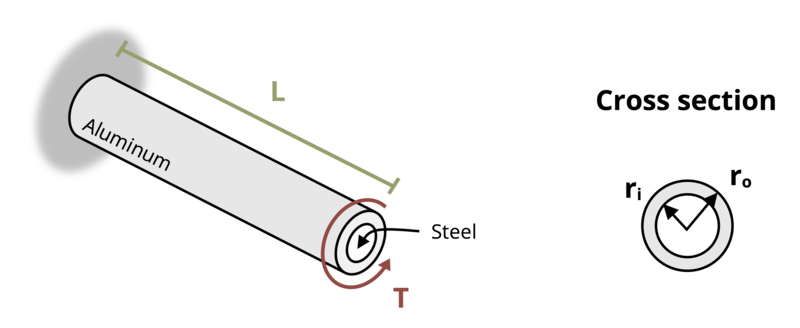
\includegraphics[keepaspectratio]{images/289.png}}

}

\caption{Figure 1: A composite circular rod is made from aluminum and
steel.}

\end{figure}%

{[}Problem adapted from © Kurt Gramoll CC BY NC-SA 4.0{]}

\begin{Shaded}
\begin{Highlighting}[]
\NormalTok{\#| standalone: true}
\NormalTok{\#| viewerHeight: 600}
\NormalTok{\#| components: [viewer]}

\NormalTok{from shiny import App, render, ui, reactive}
\NormalTok{import random}
\NormalTok{import asyncio}
\NormalTok{import io}
\NormalTok{import math}
\NormalTok{import string}
\NormalTok{from datetime import datetime}
\NormalTok{from pathlib import Path}

\NormalTok{def generate\_random\_letters(length):}
\NormalTok{    \# Generate a random string of letters of specified length}
\NormalTok{    return "".join(random.choice(string.ascii\_lowercase) for \_ in range(length))}

\NormalTok{problem\_ID = "289"}
\NormalTok{T = reactive.Value("\_\_")}
\NormalTok{L = reactive.Value("\_\_")}
\NormalTok{ro = reactive.Value("\_\_")}
\NormalTok{ri = reactive.Value("\_\_")}
\NormalTok{GA = 3800000}
\NormalTok{GS = 11000000}

\NormalTok{attempts = ["Timestamp,Attempt,Answer,Feedback\textbackslash{}n"]}

\NormalTok{app\_ui = ui.page\_fluid(}

\NormalTok{    \#ui.input\_text("ID", "", placeholder="Enter ID Number Here"),}

\NormalTok{    ui.markdown("**Problem Statement**"),}
\NormalTok{    ui.output\_ui("ui\_problem\_statement"),}
\NormalTok{    ui.input\_text(}
\NormalTok{        "answer", "Your Answer in units of ksi", placeholder="Please enter your answer"}
\NormalTok{    ),}
\NormalTok{    ui.input\_action\_button("submit", "Check Answer", class\_="btn{-}primary"),}
\NormalTok{    \#ui.download\_button("download", "Download File to Submit", class\_="btn{-}success"),}
\NormalTok{)}

\NormalTok{def server(input, output, session):}
\NormalTok{    \# Initialize a counter for attempts}
\NormalTok{    attempt\_counter = reactive.Value(0)}

\NormalTok{    @output}
\NormalTok{    @render.ui}
\NormalTok{    def ui\_problem\_statement():}
\NormalTok{        randomize\_vars()}
\NormalTok{        return [}
\NormalTok{            ui.markdown(}
\NormalTok{                f"A composite circular rod is made from aluminum (G = 3,800 ksi) and steel (G = 11,000 ksi) as shown. A torque T = \{T()\} lb{-}ft is applied to the free end. What is the maximum stress in either material? Assume length L = \{L()\} in., outer radius r\textless{}sub\textgreater{}o\textless{}/sub\textgreater{} = \{ro()\} in., and inner radius r\textless{}sub\textgreater{}i\textless{}/sub\textgreater{} = \{ri()\} in."}
\NormalTok{            )}
\NormalTok{        ]}

\NormalTok{    \#@reactive.Effect}
\NormalTok{    \#@reactive.event(input.generate\_problem)}
\NormalTok{    def randomize\_vars():}
\NormalTok{        random.seed(101)}
\NormalTok{        T.set(random.randrange(300, 2000, 100))}
\NormalTok{        L.set(random.randrange(10, 60, 1))}
\NormalTok{        ro.set(random.randrange(10, 60, 1) / 10)}
\NormalTok{        ri.set(round(ro() / 1.5, 1))}

\NormalTok{    @reactive.Effect}
\NormalTok{    @reactive.event(input.submit)}
\NormalTok{    def \_():}
\NormalTok{        attempt\_counter.set(}
\NormalTok{            attempt\_counter() + 1}
\NormalTok{        )  \# Increment the attempt counter on each submission.}
\NormalTok{        JS = math.pi * ri() ** 4 / 2}
\NormalTok{        JA = math.pi / 2 * (ro() ** 4 {-} ri() ** 4)}
\NormalTok{        TA = T() * 12 * GA * JA / (GS * JS + GA * JA)}
\NormalTok{        TS = T() * 12 {-} TA}
\NormalTok{        instr = TS * ri() / JS / 1000}
\NormalTok{        if math.isclose(float(input.answer()), instr, rel\_tol=0.01):}
\NormalTok{            check = "*Correct*"}
\NormalTok{            correct\_indicator = "JL"}
\NormalTok{        else:}
\NormalTok{            check = "*Not Correct.*"}
\NormalTok{            correct\_indicator = "JG"}

\NormalTok{        \# Generate random parts for the encoded attempt.}
\NormalTok{        random\_start = generate\_random\_letters(4)}
\NormalTok{        random\_middle = generate\_random\_letters(4)}
\NormalTok{        random\_end = generate\_random\_letters(4)}
\NormalTok{        \#encoded\_attempt = f"\{random\_start\}\{problem\_ID\}{-}\{random\_middle\}\{attempt\_counter()\}\{correct\_indicator\}{-}\{random\_end\}\{input.ID()\}"}

\NormalTok{        \# Store the most recent encoded attempt in a reactive value so it persists across submissions}
\NormalTok{        \#session.encoded\_attempt = reactive.Value(encoded\_attempt)}

\NormalTok{        \# Append the attempt data to the attempts list without the encoded attempt}
\NormalTok{        attempts.append(}
\NormalTok{            f"\{datetime.now()\}, \{attempt\_counter()\}, \{input.answer()\}, \{check\}\textbackslash{}n"}
\NormalTok{        )}

\NormalTok{        \# Show feedback to the user.}
\NormalTok{        feedback = ui.markdown(}
\NormalTok{            f"Your answer of \{input.answer()\} is \{check\}.")}
\NormalTok{        m = ui.modal(feedback, title="Feedback", easy\_close=True)}
\NormalTok{        ui.modal\_show(m)}

\NormalTok{    \#@render.download(filename=lambda: f"Problem\_Log{-}\{problem\_ID\}{-}\{input.ID()\}.csv")}
\NormalTok{    async def download():}
\NormalTok{        \# Start the CSV with the encoded attempt (without label)}
\NormalTok{        final\_encoded = (}
\NormalTok{            session.encoded\_attempt()}
\NormalTok{            if session.encoded\_attempt is not None}
\NormalTok{            else "No attempts"}
\NormalTok{        )}
\NormalTok{        yield f"\{final\_encoded\}\textbackslash{}n\textbackslash{}n"}

\NormalTok{        \# Write the header for the remaining CSV data once}
\NormalTok{        yield "Timestamp,Attempt,Answer,Feedback\textbackslash{}n"}

\NormalTok{        \# Write the attempts data, ensure that the header from the attempts list is not written again}
\NormalTok{        for attempt in attempts[1:]:  \# Skip the first element which is the header}
\NormalTok{            await asyncio.sleep(}
\NormalTok{                0.25}
\NormalTok{            )  \# This delay may not be necessary; adjust as needed}
\NormalTok{            yield attempt}


\NormalTok{\# App installation}
\NormalTok{app = App(app\_ui, server)}
\end{Highlighting}
\end{Shaded}

\chapter*{Problem 6.30 - Statically Indeterminate
Torsion}\label{problem-6.30---statically-indeterminate-torsion}
\addcontentsline{toc}{chapter}{Problem 6.30 - Statically Indeterminate
Torsion}

\markboth{Problem 6.30 - Statically Indeterminate Torsion}{Problem 6.30
- Statically Indeterminate Torsion}

\pandocbounded{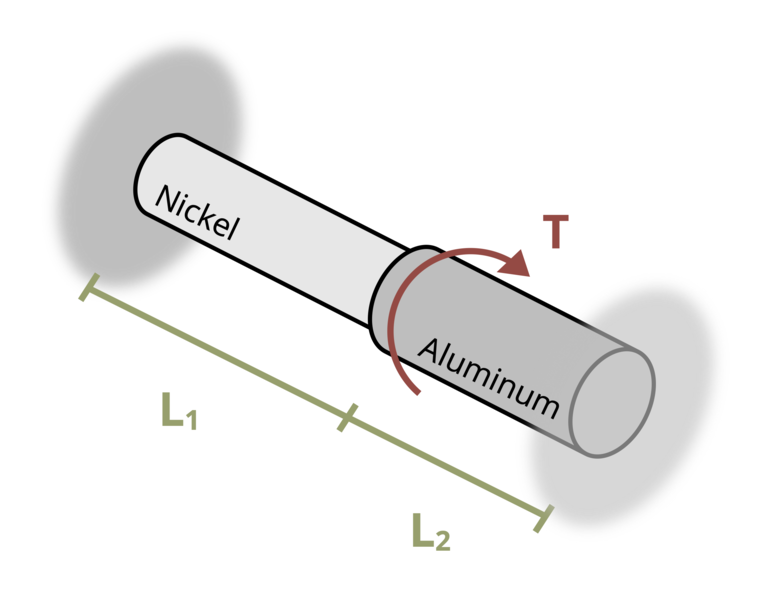
\includegraphics[keepaspectratio]{images/292.png}}
{[}Problem adapted from © Kurt Gramoll CC BY NC-SA 4.0{]}

\begin{Shaded}
\begin{Highlighting}[]
\NormalTok{\#| standalone: true}
\NormalTok{\#| viewerHeight: 600}
\NormalTok{\#| components: [viewer]}

\NormalTok{from shiny import App, render, ui, reactive}
\NormalTok{import random}
\NormalTok{import asyncio}
\NormalTok{import io}
\NormalTok{import math}
\NormalTok{import string}
\NormalTok{from datetime import datetime}
\NormalTok{from pathlib import Path}

\NormalTok{def generate\_random\_letters(length):}
\NormalTok{    \# Generate a random string of letters of specified length}
\NormalTok{    return \textquotesingle{}\textquotesingle{}.join(random.choice(string.ascii\_lowercase) for \_ in range(length)) }

\NormalTok{problem\_ID="292"}
\NormalTok{T=reactive.Value("\_\_")}
\NormalTok{d1=reactive.Value("\_\_")}
\NormalTok{d2=reactive.Value("\_\_")}
\NormalTok{L1=reactive.Value("\_\_")}
\NormalTok{L2=reactive.Value("\_\_")}
\NormalTok{Gn = 11.4e6}
\NormalTok{Ga = 4e6}

\NormalTok{attempts=["Timestamp,Attempt,Answer,Feedback\textbackslash{}n"]}

\NormalTok{app\_ui = ui.page\_fluid(}
\NormalTok{    \#ui.markdown("**Please enter your ID number from your instructor and click to generate your problem**"),}
\NormalTok{    \#ui.input\_text("ID","", placeholder="Enter ID Number Here"),}
\NormalTok{    \#ui.input\_action\_button("generate\_problem", "Generate Problem", class\_="btn{-}primary"),}
\NormalTok{    ui.markdown("**Problem Statement**"),}
\NormalTok{    ui.output\_ui("ui\_problem\_statement"),}
\NormalTok{    ui.input\_text("answer","Your Answer in units of psi", placeholder="Please enter your answer"),}
\NormalTok{    ui.input\_action\_button("submit", "Check Answer", class\_="btn{-}primary"),}
\NormalTok{    \#ui.download\_button("download", "Download File to Submit", class\_="btn{-}success"),}
\NormalTok{)}


\NormalTok{def server(input, output, session):}
\NormalTok{    \# Initialize a counter for attempts}
\NormalTok{    attempt\_counter = reactive.Value(0)}

\NormalTok{    @output}
\NormalTok{    @render.ui}
\NormalTok{    def ui\_problem\_statement():}
\NormalTok{        randomize\_vars()}
\NormalTok{        return[ui.markdown(f"A shaft is fixed between two walls. One portion is made from nickel (G\textless{}sub\textgreater{}nickel\textless{}/sub\textgreater{} = 11.4 x 10\textless{}sup\textgreater{}6\textless{}/sup\textgreater{} psi) with a diameter of d\textless{}sub\textgreater{}1\textless{}/sub\textgreater{} = \{d1()\} in. The other portion is aluminum (G\textless{}sub\textgreater{}aluminum\textless{}/sub\textgreater{} = 4 x 10\textless{}sup\textgreater{}6\textless{}/sup\textgreater{} psi) with a diameter of d\textless{}sub\textgreater{}2\textless{}/sub\textgreater{} = \{d2()\} in. A torque T = \{T()\} lb{-}ft is applied at the point where the two materials meet. If lengths L\textless{}sub\textgreater{}1\textless{}/sub\textgreater{} = \{L1()\} ft and L\textless{}sub\textgreater{}2\textless{}/sub\textgreater{} = \{L2()\} ft, what is the maximum shear stress in the shaft?")]}
    
\NormalTok{    \#@reactive.Effect}
\NormalTok{    \#@reactive.event(input.generate\_problem)}
\NormalTok{    def randomize\_vars():}
\NormalTok{        random.seed(101)}
\NormalTok{        d1.set(random.randrange(10, 60, 1)/10)}
\NormalTok{        d2.set(round(d1()*2, 2))}
\NormalTok{        T.set(random.randrange(500, 2000, 100))}
\NormalTok{        L1.set(random.randrange(4, 20, 2))}
\NormalTok{        L2.set(L1()/2)}
        
\NormalTok{    @reactive.Effect}
\NormalTok{    @reactive.event(input.submit)}
\NormalTok{    def \_():}
\NormalTok{        attempt\_counter.set(attempt\_counter() + 1)  \# Increment the attempt counter on each submission.}
\NormalTok{        Jn = (math.pi/2)*(d1()/2)**4}
\NormalTok{        Ja = (math.pi/2)*(d2()/2)**4}
\NormalTok{        TN = T()*12*L2()*12*Gn*Jn/(L1()*12*Ga*Ja+L2()*12*Gn*Jn)}
\NormalTok{        TA = T()*12{-}TN}
\NormalTok{        tauA = TA*d2()/2/Ja}
\NormalTok{        tauN = TN*d1()/2/Jn}
\NormalTok{        if tauA\textgreater{}=tauN:}
\NormalTok{            instr = tauA}
\NormalTok{        else:}
\NormalTok{            instr = tauN}
\NormalTok{        if math.isclose(float(input.answer()), instr, rel\_tol=0.01):}
\NormalTok{            check = "*Correct*"}
\NormalTok{            correct\_indicator = "JL"}
\NormalTok{        else:}
\NormalTok{            check = "*Not Correct.*"}
\NormalTok{            correct\_indicator = "JG"}

\NormalTok{        \# Generate random parts for the encoded attempt.}
\NormalTok{        random\_start = generate\_random\_letters(4)}
\NormalTok{        random\_middle = generate\_random\_letters(4)}
\NormalTok{        random\_end = generate\_random\_letters(4)}
\NormalTok{        \#encoded\_attempt = f"\{random\_start\}\{problem\_ID\}{-}\{random\_middle\}\{attempt\_counter()\}\{correct\_indicator\}{-}\{random\_end\}\{input.ID()\}"}

\NormalTok{        \# Store the most recent encoded attempt in a reactive value so it persists across submissions}
\NormalTok{        \#session.encoded\_attempt = reactive.Value(encoded\_attempt)}

\NormalTok{        \# Append the attempt data to the attempts list without the encoded attempt}
\NormalTok{        attempts.append(f"\{datetime.now()\}, \{attempt\_counter()\}, \{input.answer()\}, \{check\}\textbackslash{}n")}

\NormalTok{        \# Show feedback to the user.}
\NormalTok{        feedback = ui.markdown(f"Your answer of \{input.answer()\} is \{check\}.")}
\NormalTok{        m = ui.modal(}
\NormalTok{            feedback,}
\NormalTok{            title="Feedback",}
\NormalTok{            easy\_close=True}
\NormalTok{        )}
\NormalTok{        ui.modal\_show(m)}

\NormalTok{    \#@render.download(filename=lambda: f"Problem\_Log{-}\{problem\_ID\}{-}\{input.ID()\}.csv")}
\NormalTok{    async def download():}
\NormalTok{        \# Start the CSV with the encoded attempt (without label)}
\NormalTok{        final\_encoded = session.encoded\_attempt() if session.encoded\_attempt is not None else "No attempts"}
\NormalTok{        yield f"\{final\_encoded\}\textbackslash{}n\textbackslash{}n"}
        
\NormalTok{        \# Write the header for the remaining CSV data once}
\NormalTok{        yield "Timestamp,Attempt,Answer,Feedback\textbackslash{}n"}
        
\NormalTok{        \# Write the attempts data, ensure that the header from the attempts list is not written again}
\NormalTok{        for attempt in attempts[1:]:  \# Skip the first element which is the header}
\NormalTok{            await asyncio.sleep(0.25)  \# This delay may not be necessary; adjust as needed}
\NormalTok{            yield attempt}

\NormalTok{\# App installation}
\NormalTok{app = App(app\_ui, server)}
\end{Highlighting}
\end{Shaded}

\chapter*{Problem 6.31 - Statically Indeterminate
Torsion}\label{problem-6.31---statically-indeterminate-torsion}
\addcontentsline{toc}{chapter}{Problem 6.31 - Statically Indeterminate
Torsion}

\markboth{Problem 6.31 - Statically Indeterminate Torsion}{Problem 6.31
- Statically Indeterminate Torsion}

\pandocbounded{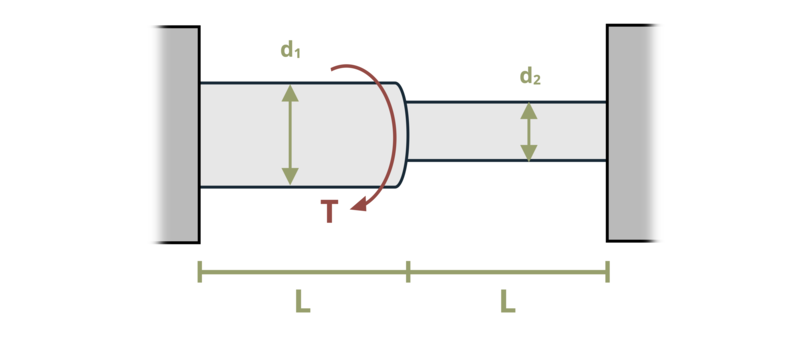
\includegraphics[keepaspectratio]{images/293.png}}
{[}Problem adapted from © Kurt Gramoll CC BY NC-SA 4.0{]}

\begin{Shaded}
\begin{Highlighting}[]
\NormalTok{\#| standalone: true}
\NormalTok{\#| viewerHeight: 600}
\NormalTok{\#| components: [viewer]}

\NormalTok{from shiny import App, render, ui, reactive}
\NormalTok{import random}
\NormalTok{import asyncio}
\NormalTok{import io}
\NormalTok{import math}
\NormalTok{import string}
\NormalTok{from datetime import datetime}
\NormalTok{from pathlib import Path}

\NormalTok{def generate\_random\_letters(length):}
\NormalTok{    \# Generate a random string of letters of specified length}
\NormalTok{    return \textquotesingle{}\textquotesingle{}.join(random.choice(string.ascii\_lowercase) for \_ in range(length)) }

\NormalTok{problem\_ID="293"}
\NormalTok{T=reactive.Value("\_\_")}
\NormalTok{d1=reactive.Value("\_\_")}
\NormalTok{d2=reactive.Value("\_\_")}
\NormalTok{L=reactive.Value("\_\_")}
\NormalTok{G = 80}

\NormalTok{attempts=["Timestamp,Attempt,Answer,Feedback\textbackslash{}n"]}

\NormalTok{app\_ui = ui.page\_fluid(}
\NormalTok{    \#ui.markdown("**Please enter your ID number from your instructor and click to generate your problem**"),}
\NormalTok{    \#ui.input\_text("ID","", placeholder="Enter ID Number Here"),}
\NormalTok{    \#ui.input\_action\_button("generate\_problem", "Generate Problem", class\_="btn{-}primary"),}
\NormalTok{    ui.markdown("**Problem Statement**"),}
\NormalTok{    ui.output\_ui("ui\_problem\_statement"),}
\NormalTok{    ui.input\_text("answer","Your Answer in units of MPa", placeholder="Please enter your answer"),}
\NormalTok{    ui.input\_action\_button("submit", "Check Answer", class\_="btn{-}primary"),}
\NormalTok{    \#ui.download\_button("download", "Download File to Submit", class\_="btn{-}success"),}
\NormalTok{)}

\NormalTok{def server(input, output, session):}
\NormalTok{    \# Initialize a counter for attempts}
\NormalTok{    attempt\_counter = reactive.Value(0)}

\NormalTok{    @output}
\NormalTok{    @render.ui}
\NormalTok{    def ui\_problem\_statement():}
\NormalTok{        randomize\_vars()}
\NormalTok{        return[ui.markdown(f"Two steel (G = 80 GPa) circular rods are firmly welded together and attached between two walls. Assume d\textless{}sub\textgreater{}1\textless{}/sub\textgreater{} = \{d1()\} mm, d\textless{}sub\textgreater{}2\textless{}/sub\textgreater{} = \{d2()\} mm, and L  = \{L()\} mm. A torque T = \{T()\} N{-}m is applied at the welded joint as shown. What is the highest stress in either rod?")]}
    
\NormalTok{    \#@reactive.Effect}
\NormalTok{    \#@reactive.event(input.generate\_problem)}
\NormalTok{    def randomize\_vars():}
\NormalTok{        random.seed(101)}
\NormalTok{        d1.set(random.randrange(20, 50, 1))}
\NormalTok{        d2.set(round(d1()*.8, 2))}
\NormalTok{        L.set(random.randrange(100, 800, 10))}
\NormalTok{        T.set(random.randrange(10, 300, 5))}
        
\NormalTok{    @reactive.Effect}
\NormalTok{    @reactive.event(input.submit)}
\NormalTok{    def \_():}
\NormalTok{        attempt\_counter.set(attempt\_counter() + 1)  \# Increment the attempt counter on each submission.}
\NormalTok{        J1 = (math.pi/2)*(d1()/2000)**4}
\NormalTok{        J2 = (math.pi/2)*(d2()/2000)**4}
\NormalTok{        RHS = J1/J2}
\NormalTok{        Tb = (T()/(RHS+1))}
\NormalTok{        Ta = T() {-} Tb}
\NormalTok{        tauA = (Ta*d1()/2000/J1)/10**6}
\NormalTok{        tauB = (Tb*d2()/2000/J2)/10**6}
\NormalTok{        if tauA\textgreater{}=tauB:}
\NormalTok{            instr = tauA}
\NormalTok{        else:}
\NormalTok{            instr = tauB}
\NormalTok{        if math.isclose(float(input.answer()), instr, rel\_tol=0.01):}
\NormalTok{            check = "*Correct*"}
\NormalTok{            correct\_indicator = "JL"}
\NormalTok{        else:}
\NormalTok{            check = "*Not Correct.*"}
\NormalTok{            correct\_indicator = "JG"}

\NormalTok{        \# Generate random parts for the encoded attempt.}
\NormalTok{        random\_start = generate\_random\_letters(4)}
\NormalTok{        random\_middle = generate\_random\_letters(4)}
\NormalTok{        random\_end = generate\_random\_letters(4)}
\NormalTok{        \#encoded\_attempt = f"\{random\_start\}\{problem\_ID\}{-}\{random\_middle\}\{attempt\_counter()\}\{correct\_indicator\}{-}\{random\_end\}\{input.ID()\}"}

\NormalTok{        \# Store the most recent encoded attempt in a reactive value so it persists across submissions}
\NormalTok{        \#session.encoded\_attempt = reactive.Value(encoded\_attempt)}

\NormalTok{        \# Append the attempt data to the attempts list without the encoded attempt}
\NormalTok{        attempts.append(f"\{datetime.now()\}, \{attempt\_counter()\}, \{input.answer()\}, \{check\}\textbackslash{}n")}

\NormalTok{        \# Show feedback to the user.}
\NormalTok{        feedback = ui.markdown(f"Your answer of \{input.answer()\} is \{check\}.")}
\NormalTok{        m = ui.modal(}
\NormalTok{            feedback,}
\NormalTok{            title="Feedback",}
\NormalTok{            easy\_close=True}
\NormalTok{        )}
\NormalTok{        ui.modal\_show(m)}

\NormalTok{    \#@render.download(filename=lambda: f"Problem\_Log{-}\{problem\_ID\}{-}\{input.ID()\}.csv")}
\NormalTok{    async def download():}
\NormalTok{        \# Start the CSV with the encoded attempt (without label)}
\NormalTok{        final\_encoded = session.encoded\_attempt() if session.encoded\_attempt is not None else "No attempts"}
\NormalTok{        yield f"\{final\_encoded\}\textbackslash{}n\textbackslash{}n"}
        
\NormalTok{        \# Write the header for the remaining CSV data once}
\NormalTok{        yield "Timestamp,Attempt,Answer,Feedback\textbackslash{}n"}
        
\NormalTok{        \# Write the attempts data, ensure that the header from the attempts list is not written again}
\NormalTok{        for attempt in attempts[1:]:  \# Skip the first element which is the header}
\NormalTok{            await asyncio.sleep(0.25)  \# This delay may not be necessary; adjust as needed}
\NormalTok{            yield attempt}

\NormalTok{\# App installation}
\NormalTok{app = App(app\_ui, server)}
\end{Highlighting}
\end{Shaded}

\chapter*{Problem 6.32 - Statically Indeterminate
Torsion}\label{problem-6.32---statically-indeterminate-torsion}
\addcontentsline{toc}{chapter}{Problem 6.32 - Statically Indeterminate
Torsion}

\markboth{Problem 6.32 - Statically Indeterminate Torsion}{Problem 6.32
- Statically Indeterminate Torsion}

\pandocbounded{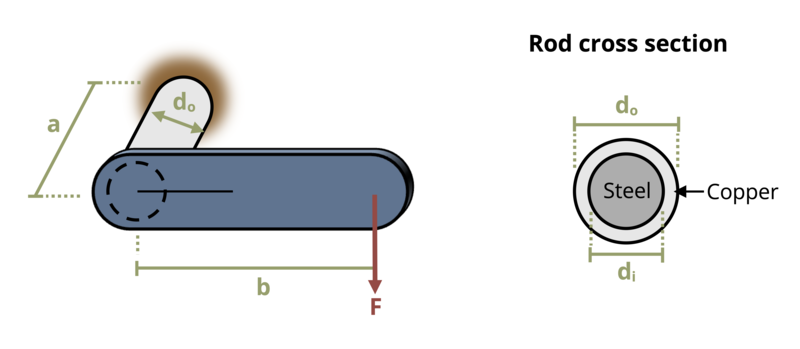
\includegraphics[keepaspectratio]{images/294.png}}
{[}Problem adapted from © Kurt Gramoll CC BY NC-SA 4.0{]}

\begin{Shaded}
\begin{Highlighting}[]
\NormalTok{\#| standalone: true}
\NormalTok{\#| viewerHeight: 600}
\NormalTok{\#| components: [viewer]}

\NormalTok{from shiny import App, render, ui, reactive}
\NormalTok{import random}
\NormalTok{import asyncio}
\NormalTok{import io}
\NormalTok{import math}
\NormalTok{import string}
\NormalTok{from datetime import datetime}
\NormalTok{from pathlib import Path}

\NormalTok{def generate\_random\_letters(length):}
\NormalTok{    \# Generate a random string of letters of specified length}
\NormalTok{    return \textquotesingle{}\textquotesingle{}.join(random.choice(string.ascii\_lowercase) for \_ in range(length))  }

\NormalTok{problem\_ID="294"}
\NormalTok{F=reactive.Value("\_\_")}
\NormalTok{di=reactive.Value("\_\_")}
\NormalTok{do=reactive.Value("\_\_")}
\NormalTok{a=reactive.Value("\_\_")}
\NormalTok{b=reactive.Value("\_\_")}
  
\NormalTok{attempts=["Timestamp,Attempt,Answer,Feedback\textbackslash{}n"]}

\NormalTok{app\_ui = ui.page\_fluid(}
\NormalTok{    \#ui.markdown("**Please enter your ID number from your instructor and click to generate your problem**"),}
\NormalTok{    \#ui.input\_text("ID","", placeholder="Enter ID Number Here"),}
\NormalTok{    \#ui.input\_action\_button("generate\_problem", "Generate Problem", class\_="btn{-}primary"),}
\NormalTok{    ui.markdown("**Problem Statement**"),}
\NormalTok{    ui.output\_ui("ui\_problem\_statement"),}
\NormalTok{    ui.input\_text("answer","Your Answer in units of MPa", placeholder="Please enter your answer"),}
\NormalTok{    ui.input\_action\_button("submit", "Check Answer", class\_="btn{-}primary"),}
\NormalTok{    \#ui.download\_button("download", "Download File to Submit", class\_="btn{-}success"),}
\NormalTok{)}

\NormalTok{def server(input, output, session):}
\NormalTok{    \# Initialize a counter for attempts}
\NormalTok{    attempt\_counter = reactive.Value(0)}

\NormalTok{    @output}
\NormalTok{    @render.ui}
\NormalTok{    def ui\_problem\_statement():}
\NormalTok{        randomize\_vars()}
\NormalTok{        return[ui.markdown(f"A load F = \{F()\} kN is applied to a bracket that is firmly attached to a wall. The rod is composed of a solid steel (G = 80 GPa) inner rod of diameter d\textless{}sub\textgreater{}i\textless{}/sub\textgreater{} = \{di()\} mm rigidly bonded to a copper (G = 48 GPa) outer casing of diameter d\textless{}sub\textgreater{}o\textless{}/sub\textgreater{} = \{do()\} mm. Determine the maximum shear stress in either material. Assume dimensions a = \{a()\} mm and b = \{b()\} mm.")]}
    
\NormalTok{    \#@reactive.Effect}
\NormalTok{    \#@reactive.event(input.generate\_problem)}
\NormalTok{    def randomize\_vars():}
\NormalTok{        random.seed(101)}
\NormalTok{        F.set(random.randrange(10,50,1)/10)}
\NormalTok{        di.set(random.randrange(25,40,1))}
\NormalTok{        do.set(di()+random.randrange(5,15,1))}
\NormalTok{        a.set(random.randrange(100,200,1))}
\NormalTok{        b.set(a()+random.randrange(30,60,1))}
        
\NormalTok{    @reactive.Effect}
\NormalTok{    @reactive.event(input.submit)}
\NormalTok{    def \_():}
\NormalTok{        attempt\_counter.set(attempt\_counter() + 1)  \# Increment the attempt counter on each submission.}
\NormalTok{        Jc = ((do()/2000)**4{-}(di()/2000)**4)*math.pi/2}
\NormalTok{        Js = (di()/2000)**4*math.pi/2}
\NormalTok{        T = F()*1000*b()/1000}
\NormalTok{        Gc = 48*10**9}
\NormalTok{        Gs = 80*10**9}
\NormalTok{        TS = T/(Jc*Gc)/(1/(Js*Gs)+1/(Jc*Gc))}
\NormalTok{        TC = T{-}TS}
\NormalTok{        tauS = TS*b()/1000/Js}
\NormalTok{        tauC = TC*do()/2000/Jc}
\NormalTok{        instr= max(tauS,tauC)/1000000}
\NormalTok{        if math.isclose(float(input.answer()), instr, rel\_tol=0.01):}
\NormalTok{            check = "*Correct*"}
\NormalTok{            correct\_indicator = "JL"}
\NormalTok{        else:}
\NormalTok{            check = "*Not Correct.*"}
\NormalTok{            correct\_indicator = "JG"}

\NormalTok{        \# Generate random parts for the encoded attempt.}
\NormalTok{        random\_start = generate\_random\_letters(4)}
\NormalTok{        random\_middle = generate\_random\_letters(4)}
\NormalTok{        random\_end = generate\_random\_letters(4)}
\NormalTok{        \#encoded\_attempt = f"\{random\_start\}\{problem\_ID\}{-}\{random\_middle\}\{attempt\_counter()\}\{correct\_indicator\}{-}\{random\_end\}\{input.ID()\}"}

\NormalTok{        \# Store the most recent encoded attempt in a reactive value so it persists across submissions}
\NormalTok{        \#session.encoded\_attempt = reactive.Value(encoded\_attempt)}

\NormalTok{        \# Append the attempt data to the attempts list without the encoded attempt}
\NormalTok{        attempts.append(f"\{datetime.now()\}, \{attempt\_counter()\}, \{input.answer()\}, \{check\}\textbackslash{}n")}

\NormalTok{        \# Show feedback to the user.}
\NormalTok{        feedback = ui.markdown(f"Your answer of \{input.answer()\} is \{check\}.")}
\NormalTok{        m = ui.modal(}
\NormalTok{            feedback,}
\NormalTok{            title="Feedback",}
\NormalTok{            easy\_close=True}
\NormalTok{        )}
\NormalTok{        ui.modal\_show(m)}

\NormalTok{    \#@render.download(filename=lambda: f"Problem\_Log{-}\{problem\_ID\}{-}\{input.ID()\}.csv")}
\NormalTok{    async def download():}
\NormalTok{        \# Start the CSV with the encoded attempt (without label)}
\NormalTok{        final\_encoded = session.encoded\_attempt() if session.encoded\_attempt is not None else "No attempts"}
\NormalTok{        yield f"\{final\_encoded\}\textbackslash{}n\textbackslash{}n"}
        
\NormalTok{        \# Write the header for the remaining CSV data once}
\NormalTok{        yield "Timestamp,Attempt,Answer,Feedback\textbackslash{}n"}
        
\NormalTok{        \# Write the attempts data, ensure that the header from the attempts list is not written again}
\NormalTok{        for attempt in attempts[1:]:  \# Skip the first element which is the header}
\NormalTok{            await asyncio.sleep(0.25)  \# This delay may not be necessary; adjust as needed}
\NormalTok{            yield attempt}
            
\NormalTok{\# App installation}
\NormalTok{app = App(app\_ui, server)}
\end{Highlighting}
\end{Shaded}

\chapter*{Problem 6.33 - Statically Indeterminate
Torsion}\label{problem-6.33---statically-indeterminate-torsion}
\addcontentsline{toc}{chapter}{Problem 6.33 - Statically Indeterminate
Torsion}

\markboth{Problem 6.33 - Statically Indeterminate Torsion}{Problem 6.33
- Statically Indeterminate Torsion}

\pandocbounded{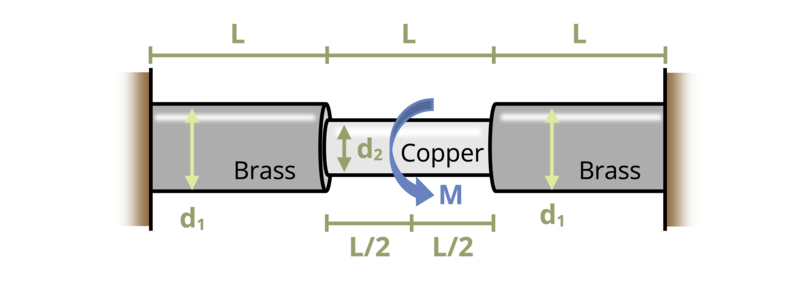
\includegraphics[keepaspectratio]{images/296.png}}
{[}Problem adapted from © Kurt Gramoll CC BY NC-SA 4.0{]}

\begin{Shaded}
\begin{Highlighting}[]
\NormalTok{\#| standalone: true}
\NormalTok{\#| viewerHeight: 600}
\NormalTok{\#| components: [viewer]}

\NormalTok{from shiny import App, render, ui, reactive}
\NormalTok{import random}
\NormalTok{import asyncio}
\NormalTok{import io}
\NormalTok{import math}
\NormalTok{import string}
\NormalTok{from datetime import datetime}
\NormalTok{from pathlib import Path}

\NormalTok{def generate\_random\_letters(length):}
\NormalTok{    \# Generate a random string of letters of specified length}
\NormalTok{    return \textquotesingle{}\textquotesingle{}.join(random.choice(string.ascii\_lowercase) for \_ in range(length))  }

\NormalTok{problem\_ID="296"}
\NormalTok{L=reactive.Value("\_\_")}
\NormalTok{d2=reactive.Value("\_\_")}
\NormalTok{d1=reactive.Value("\_\_")}
\NormalTok{T=reactive.Value("\_\_")}
  
\NormalTok{attempts=["Timestamp,Attempt,Answer,Feedback\textbackslash{}n"]}

\NormalTok{app\_ui = ui.page\_fluid(}
\NormalTok{    \#ui.markdown("**Please enter your ID number from your instructor and click to generate your problem**"),}
\NormalTok{    \#ui.input\_text("ID","", placeholder="Enter ID Number Here"),}
\NormalTok{    \#ui.input\_action\_button("generate\_problem", "Generate Problem", class\_="btn{-}primary"),}
\NormalTok{    ui.markdown("**Problem Statement**"),}
\NormalTok{    ui.output\_ui("ui\_problem\_statement"),}
\NormalTok{    ui.input\_text("answer","Your Answer in units of rad", placeholder="Please enter your answer"),}
\NormalTok{    ui.input\_action\_button("submit", "Check Answer", class\_="btn{-}primary"),}
\NormalTok{    \#ui.download\_button("download", "Download File to Submit", class\_="btn{-}success"),}
\NormalTok{)}

\NormalTok{def server(input, output, session):}
\NormalTok{    \# Initialize a counter for attempts}
\NormalTok{    attempt\_counter = reactive.Value(0)}

\NormalTok{    @output}
\NormalTok{    @render.ui}
\NormalTok{    def ui\_problem\_statement():}
\NormalTok{        randomize\_vars()}
\NormalTok{        return[ui.markdown(f"Three circular rods, each of length L = \{L()\} in., are mounted between two fixed walls. The two brass (E = 15,000 ksi, ν = 0.34) rods have diameter d\textless{}sub\textgreater{}1\textless{}/sub\textgreater{} = \{d1()\} in. The copper (E = 19,000 ksi, ν = 0.33) rod has diameter d\textless{}sub\textgreater{}2\textless{}/sub\textgreater{} = \{d2()\} in. A torque T = \{T()\} kip{-}in. is applied at the center. determine the angle of twist of point B with respect to point A.")]}
    
\NormalTok{    \#@reactive.Effect}
\NormalTok{    \#@reactive.event(input.generate\_problem)}
\NormalTok{    def randomize\_vars():}
\NormalTok{        random.seed(101)}
\NormalTok{        L.set(random.randrange(5,20,1))}
\NormalTok{        d2.set(random.randrange(5,25,1)/10)}
\NormalTok{        d1.set(d2()*2)}
\NormalTok{        T.set(random.randrange(10,100,1)/10)}
        
\NormalTok{    @reactive.Effect}
\NormalTok{    @reactive.event(input.submit)}
\NormalTok{    def \_():}
\NormalTok{        attempt\_counter.set(attempt\_counter() + 1)  \# Increment the attempt counter on each submission.}
\NormalTok{        Jb = math.pi*(d1()/2)**4/2}
\NormalTok{        Jc = math.pi*(d2()/2)**4/2}
\NormalTok{        Gb = 15000000/(2*1.34)}
\NormalTok{        Gc = 19000000/(2*1.33)}
\NormalTok{        TB = T()*1000/2}
\NormalTok{        TC = TB        }
\NormalTok{        instr= TB*L()/(Gb*Jb)+TC*L()/(Gc*Jc)}
\NormalTok{        if math.isclose(float(input.answer()), instr, rel\_tol=0.01):}
\NormalTok{            check = "*Correct*"}
\NormalTok{            correct\_indicator = "JL"}
\NormalTok{        else:}
\NormalTok{            check = "*Not Correct.*"}
\NormalTok{            correct\_indicator = "JG"}

\NormalTok{        \# Generate random parts for the encoded attempt.}
\NormalTok{        random\_start = generate\_random\_letters(4)}
\NormalTok{        random\_middle = generate\_random\_letters(4)}
\NormalTok{        random\_end = generate\_random\_letters(4)}
\NormalTok{        \#encoded\_attempt = f"\{random\_start\}\{problem\_ID\}{-}\{random\_middle\}\{attempt\_counter()\}\{correct\_indicator\}{-}\{random\_end\}\{input.ID()\}"}

\NormalTok{        \# Store the most recent encoded attempt in a reactive value so it persists across submissions}
\NormalTok{        \#session.encoded\_attempt = reactive.Value(encoded\_attempt)}

\NormalTok{        \# Append the attempt data to the attempts list without the encoded attempt}
\NormalTok{        attempts.append(f"\{datetime.now()\}, \{attempt\_counter()\}, \{input.answer()\}, \{check\}\textbackslash{}n")}

\NormalTok{        \# Show feedback to the user.}
\NormalTok{        feedback = ui.markdown(f"Your answer of \{input.answer()\} is \{check\}.")}
\NormalTok{        m = ui.modal(}
\NormalTok{            feedback,}
\NormalTok{            title="Feedback",}
\NormalTok{            easy\_close=True}
\NormalTok{        )}
\NormalTok{        ui.modal\_show(m)}

\NormalTok{    \#@render.download(filename=lambda: f"Problem\_Log{-}\{problem\_ID\}{-}\{input.ID()\}.csv")}
\NormalTok{    async def download():}
\NormalTok{        \# Start the CSV with the encoded attempt (without label)}
\NormalTok{        final\_encoded = session.encoded\_attempt() if session.encoded\_attempt is not None else "No attempts"}
\NormalTok{        yield f"\{final\_encoded\}\textbackslash{}n\textbackslash{}n"}
        
\NormalTok{        \# Write the header for the remaining CSV data once}
\NormalTok{        yield "Timestamp,Attempt,Answer,Feedback\textbackslash{}n"}
        
\NormalTok{        \# Write the attempts data, ensure that the header from the attempts list is not written again}
\NormalTok{        for attempt in attempts[1:]:  \# Skip the first element which is the header}
\NormalTok{            await asyncio.sleep(0.25)  \# This delay may not be necessary; adjust as needed}
\NormalTok{            yield attempt}
            
\NormalTok{\# App installation}
\NormalTok{app = App(app\_ui, server)}
\end{Highlighting}
\end{Shaded}

\chapter*{Problem 6.34 - Statically Indeterminate
Torsion}\label{problem-6.34---statically-indeterminate-torsion}
\addcontentsline{toc}{chapter}{Problem 6.34 - Statically Indeterminate
Torsion}

\markboth{Problem 6.34 - Statically Indeterminate Torsion}{Problem 6.34
- Statically Indeterminate Torsion}

\pandocbounded{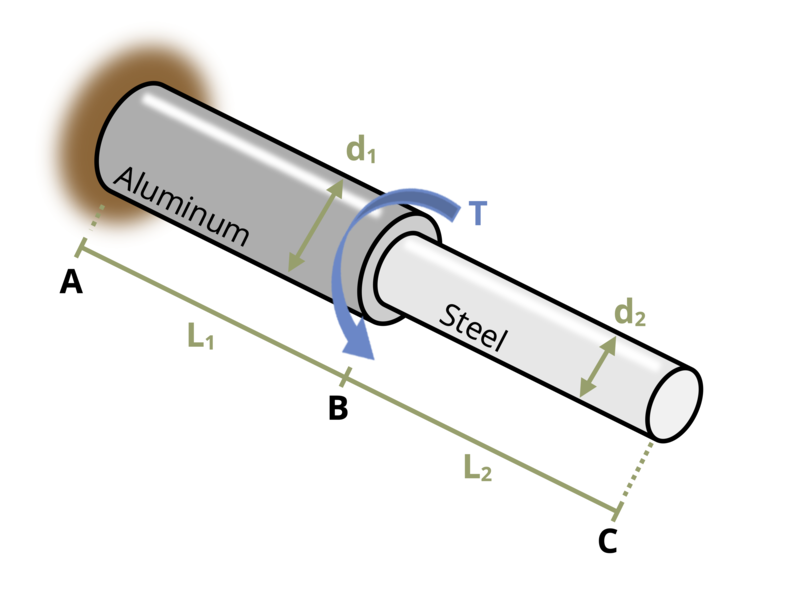
\includegraphics[keepaspectratio]{images/301.png}}
{[}Problem adapted from © Kurt Gramoll CC BY NC-SA 4.0{]}

\begin{Shaded}
\begin{Highlighting}[]
\NormalTok{\#| standalone: true}
\NormalTok{\#| viewerHeight: 600}
\NormalTok{\#| components: [viewer]}

\NormalTok{from shiny import App, render, ui, reactive}
\NormalTok{import random}
\NormalTok{import asyncio}
\NormalTok{import io}
\NormalTok{import math}
\NormalTok{import string}
\NormalTok{from datetime import datetime}
\NormalTok{from pathlib import Path}

\NormalTok{def generate\_random\_letters(length):}
\NormalTok{    \# Generate a random string of letters of specified length}
\NormalTok{    return \textquotesingle{}\textquotesingle{}.join(random.choice(string.ascii\_lowercase) for \_ in range(length))  }

\NormalTok{problem\_ID="301"}
\NormalTok{L1=reactive.Value("\_\_")}
\NormalTok{L2=reactive.Value("\_\_")}
\NormalTok{d2=reactive.Value("\_\_")}
\NormalTok{d1=reactive.Value("\_\_")}
\NormalTok{angle=reactive.Value("\_\_")}
  
\NormalTok{attempts=["Timestamp,Attempt,Answer,Feedback\textbackslash{}n"]}

\NormalTok{app\_ui = ui.page\_fluid(}
\NormalTok{    \#ui.markdown("**Please enter your ID number from your instructor and click to generate your problem**"),}
\NormalTok{    \#ui.input\_text("ID","", placeholder="Enter ID Number Here"),}
\NormalTok{    \#ui.input\_action\_button("generate\_problem", "Generate Problem", class\_="btn{-}primary"),}
\NormalTok{    ui.markdown("**Problem Statement**"),}
\NormalTok{    ui.output\_ui("ui\_problem\_statement"),}
\NormalTok{    ui.input\_text("answer","Your Answer in units of lb{-}in", placeholder="Please enter your answer"),}
\NormalTok{    ui.input\_action\_button("submit", "Check Answer", class\_="btn{-}primary"),}
\NormalTok{    \#ui.download\_button("download", "Download File to Submit", class\_="btn{-}success"),}
\NormalTok{)}

\NormalTok{def server(input, output, session):}
\NormalTok{    \# Initialize a counter for attempts}
\NormalTok{    attempt\_counter = reactive.Value(0)}

\NormalTok{    @output}
\NormalTok{    @render.ui}
\NormalTok{    def ui\_problem\_statement():}
\NormalTok{        randomize\_vars()}
\NormalTok{        return[ui.markdown(f"A steel (G = 12,700 ksi) rod and an aluminum (G = 4,300 ksi) rod are attached firmly between two walls as shown. The lengths are L\textless{}sub\textgreater{}1\textless{}/sub\textgreater{} = \{L1()\} in. and L\textless{}sub\textgreater{}2\textless{}/sub\textgreater{} = \{L2()\} in., while the diameters are d\textless{}sub\textgreater{}1\textless{}/sub\textgreater{} = \{d1()\} in. and d\textless{}sub\textgreater{}2\textless{}/sub\textgreater{} = \{d2()\} in. A torque T is applied at the joint between ther rods and it is measureed that the joint rotates \{angle()\}°. Determine the magnitude of torque T.")]}
    
\NormalTok{    \#@reactive.Effect}
\NormalTok{    \#@reactive.event(input.generate\_problem)}
\NormalTok{    def randomize\_vars():}
\NormalTok{        random.seed(101)}
\NormalTok{        L1.set(random.randrange(5,25,1))}
\NormalTok{        L2.set(L1()+random.randrange(2,5,1))}
\NormalTok{        d2.set(random.randrange(50,300,5)/100)}
\NormalTok{        d1.set(d2()+random.randrange(25,100,5)/100)}
\NormalTok{        angle.set(random.randrange(10,50,1)/10)}
        
\NormalTok{    @reactive.Effect}
\NormalTok{    @reactive.event(input.submit)}
\NormalTok{    def \_():}
\NormalTok{        attempt\_counter.set(attempt\_counter() + 1)  \# Increment the attempt counter on each submission.}
\NormalTok{        Js = math.pi*(d2()/2)**4/2}
\NormalTok{        Jal = math.pi*(d1()/2)**4/2}
\NormalTok{        Ts = angle()*math.pi/180*Js*12700000/L2()}
\NormalTok{        Tal = angle()*math.pi/180*Jal*4300000/L1()}
\NormalTok{        instr= Ts+Tal}
\NormalTok{        if math.isclose(float(input.answer()), instr, rel\_tol=0.01):}
\NormalTok{            check = "*Correct*"}
\NormalTok{            correct\_indicator = "JL"}
\NormalTok{        else:}
\NormalTok{            check = "*Not Correct.*"}
\NormalTok{            correct\_indicator = "JG"}

\NormalTok{        \# Generate random parts for the encoded attempt.}
\NormalTok{        random\_start = generate\_random\_letters(4)}
\NormalTok{        random\_middle = generate\_random\_letters(4)}
\NormalTok{        random\_end = generate\_random\_letters(4)}
\NormalTok{        \#encoded\_attempt = f"\{random\_start\}\{problem\_ID\}{-}\{random\_middle\}\{attempt\_counter()\}\{correct\_indicator\}{-}\{random\_end\}\{input.ID()\}"}

\NormalTok{        \# Store the most recent encoded attempt in a reactive value so it persists across submissions}
\NormalTok{        \#session.encoded\_attempt = reactive.Value(encoded\_attempt)}

\NormalTok{        \# Append the attempt data to the attempts list without the encoded attempt}
\NormalTok{        attempts.append(f"\{datetime.now()\}, \{attempt\_counter()\}, \{input.answer()\}, \{check\}\textbackslash{}n")}

\NormalTok{        \# Show feedback to the user.}
\NormalTok{        feedback = ui.markdown(f"Your answer of \{input.answer()\} is \{check\}.")}
\NormalTok{        m = ui.modal(}
\NormalTok{            feedback,}
\NormalTok{            title="Feedback",}
\NormalTok{            easy\_close=True}
\NormalTok{        )}
\NormalTok{        ui.modal\_show(m)}

\NormalTok{    \#@render.download(filename=lambda: f"Problem\_Log{-}\{problem\_ID\}{-}\{input.ID()\}.csv")}
\NormalTok{    async def download():}
\NormalTok{        \# Start the CSV with the encoded attempt (without label)}
\NormalTok{        final\_encoded = session.encoded\_attempt() if session.encoded\_attempt is not None else "No attempts"}
\NormalTok{        yield f"\{final\_encoded\}\textbackslash{}n\textbackslash{}n"}
        
\NormalTok{        \# Write the header for the remaining CSV data once}
\NormalTok{        yield "Timestamp,Attempt,Answer,Feedback\textbackslash{}n"}
        
\NormalTok{        \# Write the attempts data, ensure that the header from the attempts list is not written again}
\NormalTok{        for attempt in attempts[1:]:  \# Skip the first element which is the header}
\NormalTok{            await asyncio.sleep(0.25)  \# This delay may not be necessary; adjust as needed}
\NormalTok{            yield attempt}
            
\NormalTok{\# App installation}
\NormalTok{app = App(app\_ui, server)}
\end{Highlighting}
\end{Shaded}

\part{Chapter 7 Problems}

\chapter*{Problem 7.1 - Internal Shear Force \& Bending Moment by
Equilibrium}\label{problem-7.1---internal-shear-force-bending-moment-by-equilibrium}
\addcontentsline{toc}{chapter}{Problem 7.1 - Internal Shear Force \&
Bending Moment by Equilibrium}

\markboth{Problem 7.1 - Internal Shear Force \& Bending Moment by
Equilibrium}{Problem 7.1 - Internal Shear Force \& Bending Moment by
Equilibrium}

\pandocbounded{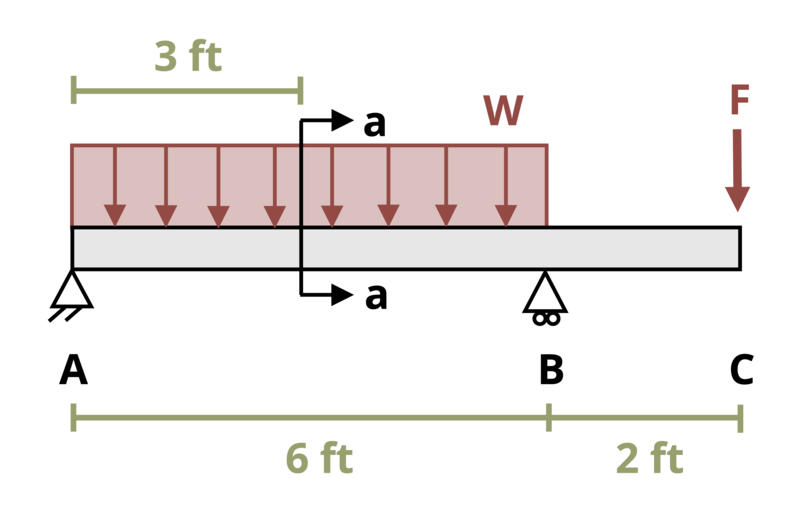
\includegraphics[keepaspectratio]{images/305.png}}
{[}Problem adapted from © Kurt Gramoll CC BY NC-SA 4.0{]}

\begin{Shaded}
\begin{Highlighting}[]
\NormalTok{\#| standalone: true}
\NormalTok{\#| viewerHeight: 600}
\NormalTok{\#| components: [viewer]}

\NormalTok{from shiny import App, render, ui, reactive}
\NormalTok{import random}
\NormalTok{import asyncio}
\NormalTok{import io}
\NormalTok{import math}
\NormalTok{import string}
\NormalTok{from datetime import datetime}
\NormalTok{from pathlib import Path}

\NormalTok{def generate\_random\_letters(length):}
\NormalTok{    return \textquotesingle{}\textquotesingle{}.join(random.choice(string.ascii\_lowercase) for \_ in range(length))}

\NormalTok{problem\_ID = "305"}
\NormalTok{w = reactive.Value("\_\_")}
\NormalTok{F = reactive.Value("\_\_")}

\NormalTok{attempts = ["Timestamp,Attempt,Answer1,Answer2,Feedback\textbackslash{}n"]}

\NormalTok{app\_ui = ui.page\_fluid(}
\NormalTok{    \#ui.markdown("**Please enter your ID number from your instructor and click to generate your problem**"),}
\NormalTok{    \#ui.input\_text("ID", "", placeholder="Enter ID Number Here"),}
\NormalTok{    \#ui.input\_action\_button("generate\_problem", "Generate Problem", class\_="btn{-}primary"),}
\NormalTok{    ui.markdown("**Problem Statement**"),}
\NormalTok{    ui.output\_ui("ui\_problem\_statement"),}
\NormalTok{    ui.input\_text("answer1", "Your internal shear force answer in units of lb", placeholder="Please enter your answer 1"),}
\NormalTok{    ui.input\_text("answer2", "Your moment answer in units of lb{-}ft", placeholder="Please enter your answer 2"),}
\NormalTok{    ui.input\_action\_button("submit", "Check Answers", class\_="btn{-}primary"),}
\NormalTok{    \#ui.download\_button("download", "Download File to Submit", class\_="btn{-}success"),}
\NormalTok{)}

\NormalTok{def server(input, output, session):}
\NormalTok{    attempt\_counter = reactive.Value(0)}

\NormalTok{    @output}
\NormalTok{    @render.ui}
\NormalTok{    def ui\_problem\_statement():}
\NormalTok{        randomize\_vars()}
\NormalTok{        return [ui.markdown(f"A beam is subjected to the loading shown, where w = \{w()\} lb/ft and F = \{F()\} lb. Determine the internal shear force and bending moment at section a{-}a.")]}

\NormalTok{    \#@reactive.Effect}
\NormalTok{    \#@reactive.event(input.generate\_problem)}
\NormalTok{    def randomize\_vars():}
\NormalTok{        random.seed(101)}
\NormalTok{        w.set(random.randrange(5, 150, 5))}
\NormalTok{        F.set(random.randrange(300, 750, 10))}

\NormalTok{    @reactive.Effect}
\NormalTok{    @reactive.event(input.submit)}
\NormalTok{    def \_():}
\NormalTok{        attempt\_counter.set(attempt\_counter() + 1)}
\NormalTok{        Ay = (F()*2 {-} w()*6*3) / {-}6}
\NormalTok{        instr1 = Ay {-} w()*3}
\NormalTok{        instr2 = Ay*3 {-} w()*3*1.5}
\NormalTok{        correct1 = math.isclose(float(input.answer1()), instr1, rel\_tol=0.01)}
\NormalTok{        correct2 = math.isclose(float(input.answer2()), instr2, rel\_tol=0.01)}
        
\NormalTok{        if correct1 and correct2:}
\NormalTok{            check = "both correct."}
\NormalTok{        elif correct1:}
\NormalTok{            check = f" \{\textquotesingle{}correct for answer 1 and incorrect for answer 2.\textquotesingle{}\}"}
\NormalTok{        elif correct2:}
\NormalTok{            check = f"\{\textquotesingle{}incorrect for answer 1 and correct for answer 2.\textquotesingle{}\}"}
\NormalTok{        else:}
\NormalTok{            check = f"\{\textquotesingle{}both incorrect.\textquotesingle{}\}"}
        
\NormalTok{        correct\_indicator = "JL" if correct1 and correct2 else "JG"}

\NormalTok{        random\_start = generate\_random\_letters(4)}
\NormalTok{        random\_middle = generate\_random\_letters(4)}
\NormalTok{        random\_end = generate\_random\_letters(4)}
\NormalTok{        \#encoded\_attempt = f"\{random\_start\}\{problem\_ID\}{-}\{random\_middle\}\{attempt\_counter()\}\{correct\_indicator\}{-}\{random\_end\}\{input.ID()\}"}

\NormalTok{        \#session.encoded\_attempt = reactive.Value(encoded\_attempt)}
\NormalTok{        attempts.append(f"\{datetime.now()\}, \{attempt\_counter()\}, \{input.answer1()\}, \{input.answer2()\}, \{check\}\textbackslash{}n")}

\NormalTok{        feedback = ui.markdown(f"Your answers of \{input.answer1()\} and \{input.answer2()\} are \{check\}.")}
\NormalTok{        m = ui.modal(feedback, title="Feedback", easy\_close=True)}
\NormalTok{        ui.modal\_show(m)}

\NormalTok{    \#@render.download(filename=lambda: f"Problem\_Log{-}\{problem\_ID\}{-}\{input.ID()\}.csv")}
\NormalTok{    async def download():}
\NormalTok{        final\_encoded = session.encoded\_attempt() if session.encoded\_attempt is not None else "No attempts"}
\NormalTok{        yield f"\{final\_encoded\}\textbackslash{}n\textbackslash{}n"}
\NormalTok{        yield "Timestamp,Attempt,Answer1,Answer2,Feedback\textbackslash{}n"}
\NormalTok{        for attempt in attempts[1:]:}
\NormalTok{            await asyncio.sleep(0.25)}
\NormalTok{            yield attempt}

\NormalTok{app = App(app\_ui, server)}
\end{Highlighting}
\end{Shaded}

\chapter*{Problem 7.2 - Internal Shear Force \& Bending Moment by
Equilibrium}\label{problem-7.2---internal-shear-force-bending-moment-by-equilibrium}
\addcontentsline{toc}{chapter}{Problem 7.2 - Internal Shear Force \&
Bending Moment by Equilibrium}

\markboth{Problem 7.2 - Internal Shear Force \& Bending Moment by
Equilibrium}{Problem 7.2 - Internal Shear Force \& Bending Moment by
Equilibrium}

\pandocbounded{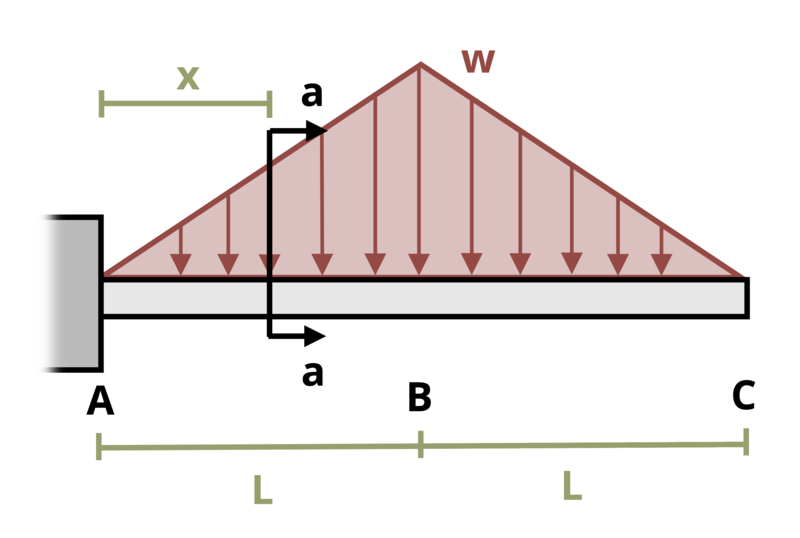
\includegraphics[keepaspectratio]{images/306.png}}
{[}Problem adapted from © Kurt Gramoll CC BY NC-SA 4.0{]}

\begin{Shaded}
\begin{Highlighting}[]
\NormalTok{\#| standalone: true}
\NormalTok{\#| viewerHeight: 600}
\NormalTok{\#| components: [viewer]}

\NormalTok{from shiny import App, render, ui, reactive}
\NormalTok{import random}
\NormalTok{import asyncio}
\NormalTok{import io}
\NormalTok{import math}
\NormalTok{import string}
\NormalTok{from datetime import datetime}
\NormalTok{from pathlib import Path}

\NormalTok{def generate\_random\_letters(length):}
\NormalTok{    \# Generate a random string of letters of specified length}
\NormalTok{    return \textquotesingle{}\textquotesingle{}.join(random.choice(string.ascii\_lowercase) for \_ in range(length)) }

\NormalTok{problem\_ID="306"}
\NormalTok{w=reactive.Value("\_\_")}
\NormalTok{L=reactive.Value("\_\_")}
\NormalTok{x=reactive.Value("\_\_")}

\NormalTok{attempts=["Timestamp,Attempt,Answer,Feedback\textbackslash{}n"]}

\NormalTok{app\_ui = ui.page\_fluid(}
\NormalTok{    \#ui.markdown("**Please enter your ID number from your instructor and click to generate your problem**"),}
\NormalTok{    \#ui.input\_text("ID","", placeholder="Enter ID Number Here"),}
\NormalTok{    \#ui.input\_action\_button("generate\_problem", "Generate Problem", class\_="btn{-}primary"),}
\NormalTok{    ui.markdown("**Problem Statement**"),}
\NormalTok{    ui.output\_ui("ui\_problem\_statement"),}
\NormalTok{    ui.input\_text("answer","Your Answer in units of kN{-}m", placeholder="Please enter your answer"),}
\NormalTok{    ui.input\_action\_button("submit", "Check Answer", class\_="btn{-}primary"),}
\NormalTok{    \#ui.download\_button("download", "Download File to Submit", class\_="btn{-}success"),}
\NormalTok{)}

\NormalTok{def server(input, output, session):}
\NormalTok{    \# Initialize a counter for attempts}
\NormalTok{    attempt\_counter = reactive.Value(0)}

\NormalTok{    @output}
\NormalTok{    @render.ui}
\NormalTok{    def ui\_problem\_statement():}
\NormalTok{        randomize\_vars()}
\NormalTok{        return[ui.markdown(f"A beam is subjected to the loading shown, where w = \{w()\} kN/m and L = \{L()\} m. What is the internal bending moment at section a{-}a at x = \{x()\} m?")]}
    
\NormalTok{    \#@reactive.Effect}
\NormalTok{    \#@reactive.event(input.generate\_problem)}
\NormalTok{    def randomize\_vars():}
\NormalTok{        random.seed(101)}
\NormalTok{        w.set(random.randrange(20, 200, 1)/20)}
\NormalTok{        L.set(random.randrange(20, 50, 2)/10)}
\NormalTok{        x.set(L()/2)}
        
\NormalTok{    @reactive.Effect}
\NormalTok{    @reactive.event(input.submit)}
\NormalTok{    def \_():}
\NormalTok{        attempt\_counter.set(attempt\_counter() + 1)  \# Increment the attempt counter on each submission.}
\NormalTok{        instr= w()*L()*x(){-}w()*L()**2{-}w()*x()**3/(6*L())}
\NormalTok{        if math.isclose(float(input.answer()), instr, rel\_tol=0.01):}
\NormalTok{            check = "*Correct*"}
\NormalTok{            correct\_indicator = "JL"}
\NormalTok{        else:}
\NormalTok{            check = "*Not Correct.*"}
\NormalTok{            correct\_indicator = "JG"}

\NormalTok{        \# Generate random parts for the encoded attempt.}
\NormalTok{        random\_start = generate\_random\_letters(4)}
\NormalTok{        random\_middle = generate\_random\_letters(4)}
\NormalTok{        random\_end = generate\_random\_letters(4)}
\NormalTok{        \#encoded\_attempt = f"\{random\_start\}\{problem\_ID\}{-}\{random\_middle\}\{attempt\_counter()\}\{correct\_indicator\}{-}\{random\_end\}\{input.ID()\}"}

\NormalTok{        \# Store the most recent encoded attempt in a reactive value so it persists across submissions}
\NormalTok{        \#session.encoded\_attempt = reactive.Value(encoded\_attempt)}

\NormalTok{        \# Append the attempt data to the attempts list without the encoded attempt}
\NormalTok{        attempts.append(f"\{datetime.now()\}, \{attempt\_counter()\}, \{input.answer()\}, \{check\}\textbackslash{}n")}

\NormalTok{        \# Show feedback to the user.}
\NormalTok{        feedback = ui.markdown(f"Your answer of \{input.answer()\} is \{check\}.")}
\NormalTok{        m = ui.modal(}
\NormalTok{            feedback,}
\NormalTok{            title="Feedback",}
\NormalTok{            easy\_close=True}
\NormalTok{        )}
\NormalTok{        ui.modal\_show(m)}

\NormalTok{    \#@render.download(filename=lambda: f"Problem\_Log{-}\{problem\_ID\}{-}\{input.ID()\}.csv")}
\NormalTok{    async def download():}
\NormalTok{        \# Start the CSV with the encoded attempt (without label)}
\NormalTok{        final\_encoded = session.encoded\_attempt() if session.encoded\_attempt is not None else "No attempts"}
\NormalTok{        yield f"\{final\_encoded\}\textbackslash{}n\textbackslash{}n"}
        
\NormalTok{        \# Write the header for the remaining CSV data once}
\NormalTok{        yield "Timestamp,Attempt,Answer,Feedback\textbackslash{}n"}
        
\NormalTok{        \# Write the attempts data, ensure that the header from the attempts list is not written again}
\NormalTok{        for attempt in attempts[1:]:  \# Skip the first element which is the header}
\NormalTok{            await asyncio.sleep(0.25)  \# This delay may not be necessary; adjust as needed}
\NormalTok{            yield attempt}

\NormalTok{\# App installation}
\NormalTok{app = App(app\_ui, server)}
\end{Highlighting}
\end{Shaded}

\chapter*{Problem 7.3 - Internal Shear Force \& Bending Moment by
Equilibrium}\label{problem-7.3---internal-shear-force-bending-moment-by-equilibrium}
\addcontentsline{toc}{chapter}{Problem 7.3 - Internal Shear Force \&
Bending Moment by Equilibrium}

\markboth{Problem 7.3 - Internal Shear Force \& Bending Moment by
Equilibrium}{Problem 7.3 - Internal Shear Force \& Bending Moment by
Equilibrium}

\pandocbounded{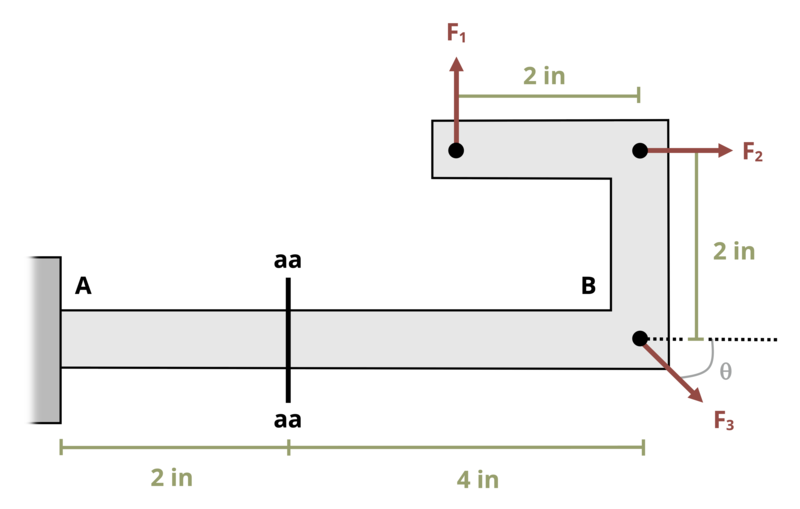
\includegraphics[keepaspectratio]{images/309.png}}
{[}Problem adapted from © Kurt Gramoll CC BY NC-SA 4.0{]}

\begin{Shaded}
\begin{Highlighting}[]
\NormalTok{\#| standalone: true}
\NormalTok{\#| viewerHeight: 600}
\NormalTok{\#| components: [viewer]}

\NormalTok{from shiny import App, render, ui, reactive}
\NormalTok{import random}
\NormalTok{import asyncio}
\NormalTok{import io}
\NormalTok{import math}
\NormalTok{import string}
\NormalTok{from datetime import datetime}
\NormalTok{from pathlib import Path}

\NormalTok{def generate\_random\_letters(length):}
\NormalTok{    return \textquotesingle{}\textquotesingle{}.join(random.choice(string.ascii\_lowercase) for \_ in range(length))}

\NormalTok{problem\_ID = "309"}
\NormalTok{F1 = reactive.Value("\_\_")}
\NormalTok{F2 = reactive.Value("\_\_")}
\NormalTok{F3 = reactive.Value("\_\_")}
\NormalTok{Θ = reactive.Value("\_\_")}

\NormalTok{attempts = ["Timestamp,Attempt,Answer1,Answer2,Feedback\textbackslash{}n"]}

\NormalTok{app\_ui = ui.page\_fluid(}
\NormalTok{    \#ui.markdown("**Please enter your ID number from your instructor and click to generate your problem**"),}
\NormalTok{    \#ui.input\_text("ID", "", placeholder="Enter ID Number Here"),}
\NormalTok{    \#ui.input\_action\_button("generate\_problem", "Generate Problem", class\_="btn{-}primary"),}
\NormalTok{    ui.markdown("**Problem Statement**"),}
\NormalTok{    ui.output\_ui("ui\_problem\_statement"),}
\NormalTok{    ui.input\_text("answer1", "Your internal shear force answer in units of lb", placeholder="Please enter your answer 1"),}
\NormalTok{    ui.input\_text("answer2", "Your moment answer in units of lb{-}in", placeholder="Please enter your answer 2"),}
\NormalTok{    ui.input\_action\_button("submit", "Check Answers", class\_="btn{-}primary"),}
\NormalTok{    \#ui.download\_button("download", "Download File to Submit", class\_="btn{-}success"),}
\NormalTok{)}

\NormalTok{def server(input, output, session):}
\NormalTok{    attempt\_counter = reactive.Value(0)}

\NormalTok{    @output}
\NormalTok{    @render.ui}
\NormalTok{    def ui\_problem\_statement():}
\NormalTok{        randomize\_vars()}
\NormalTok{        return [ui.markdown(f"Three loads are applied to the structure as shown, where F\textless{}sub\textgreater{}1\textless{}/sub\textgreater{} = \{F1()\} lb., F\textless{}sub\textgreater{}2\textless{}/sub\textgreater{} = \{F2()\} lb., and F\textless{}sub\textgreater{}3\textless{}/sub\textgreater{} = \{F3()\} lb applied at an angle Θ = \{Θ()\} °. Determine the internal shear force and bending moment at section aa.")]}

\NormalTok{    \#@reactive.Effect}
\NormalTok{    \#@reactive.event(input.generate\_problem)}
\NormalTok{    def randomize\_vars():}
\NormalTok{        random.seed(101)}
\NormalTok{        F1.set(random.randrange(10, 30, 1))}
\NormalTok{        F2.set(random.randrange(10, 30, 1))}
\NormalTok{        F3.set(random.randrange(10, 30, 1))}
\NormalTok{        Θ.set(random.randrange(45, 55, 1))}

\NormalTok{    @reactive.Effect}
\NormalTok{    @reactive.event(input.submit)}
\NormalTok{    def \_():}
\NormalTok{        attempt\_counter.set(attempt\_counter() + 1)}
\NormalTok{        instr1 = {-}F3() + F3()*math.sin(math.radians(Θ()))}
\NormalTok{        instr2 = 2*F1() {-} 2*F2() {-} 4*F3()*math.sin(math.radians(Θ()))}
\NormalTok{        correct1 = math.isclose(float(input.answer1()), instr1, rel\_tol=0.01)}
\NormalTok{        correct2 = math.isclose(float(input.answer2()), instr2, rel\_tol=0.01)}
        
\NormalTok{        if correct1 and correct2:}
\NormalTok{            check = "both correct."}
\NormalTok{        elif correct1:}
\NormalTok{            check = f" \{\textquotesingle{}correct for answer 1 and incorrect for answer 2.\textquotesingle{}\}"}
\NormalTok{        elif correct2:}
\NormalTok{            check = f"\{\textquotesingle{}incorrect for answer 1 and correct for answer 2.\textquotesingle{}\}"}
\NormalTok{        else:}
\NormalTok{            check = f"\{\textquotesingle{}both incorrect.\textquotesingle{}\}"}
        
\NormalTok{        correct\_indicator = "JL" if correct1 and correct2 else "JG"}

\NormalTok{        random\_start = generate\_random\_letters(4)}
\NormalTok{        random\_middle = generate\_random\_letters(4)}
\NormalTok{        random\_end = generate\_random\_letters(4)}
\NormalTok{        \#encoded\_attempt = f"\{random\_start\}\{problem\_ID\}{-}\{random\_middle\}\{attempt\_counter()\}\{correct\_indicator\}{-}\{random\_end\}\{input.ID()\}"}

\NormalTok{        \#session.encoded\_attempt = reactive.Value(encoded\_attempt)}
\NormalTok{        attempts.append(f"\{datetime.now()\}, \{attempt\_counter()\}, \{input.answer1()\}, \{input.answer2()\}, \{check\}\textbackslash{}n")}

\NormalTok{        feedback = ui.markdown(f"Your answers of \{input.answer1()\} and \{input.answer2()\} are \{check\}.")}
\NormalTok{        m = ui.modal(feedback, title="Feedback", easy\_close=True)}
\NormalTok{        ui.modal\_show(m)}

\NormalTok{    \#@render.download(filename=lambda: f"Problem\_Log{-}\{problem\_ID\}{-}\{input.ID()\}.csv")}
\NormalTok{    async def download():}
\NormalTok{        final\_encoded = session.encoded\_attempt() if session.encoded\_attempt is not None else "No attempts"}
\NormalTok{        yield f"\{final\_encoded\}\textbackslash{}n\textbackslash{}n"}
\NormalTok{        yield "Timestamp,Attempt,Answer1,Answer2,Feedback\textbackslash{}n"}
\NormalTok{        for attempt in attempts[1:]:}
\NormalTok{            await asyncio.sleep(0.25)}
\NormalTok{            yield attempt}

\NormalTok{app = App(app\_ui, server)}
\end{Highlighting}
\end{Shaded}

\chapter*{Problem 7.4 - Internal Shear Force \& Bending Moments by
Equilibrium}\label{problem-7.4---internal-shear-force-bending-moments-by-equilibrium}
\addcontentsline{toc}{chapter}{Problem 7.4 - Internal Shear Force \&
Bending Moments by Equilibrium}

\markboth{Problem 7.4 - Internal Shear Force \& Bending Moments by
Equilibrium}{Problem 7.4 - Internal Shear Force \& Bending Moments by
Equilibrium}

\pandocbounded{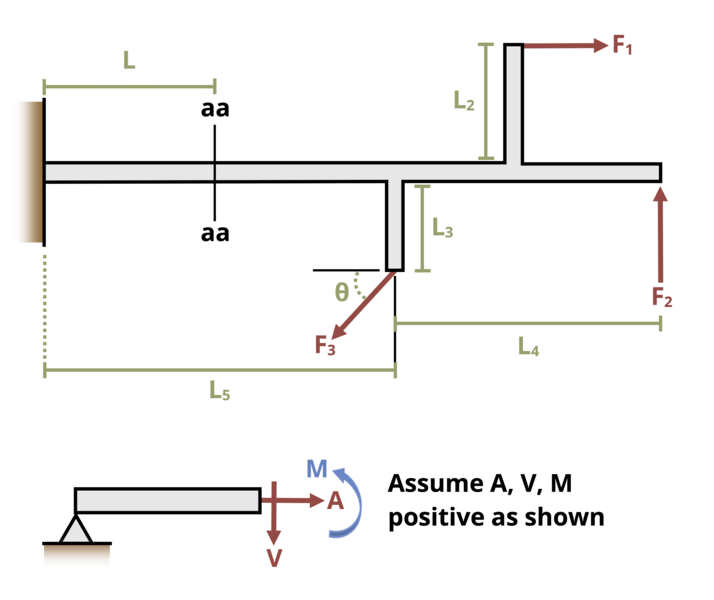
\includegraphics[keepaspectratio]{images/311.png}}
{[}Problem adapted from © Kurt Gramoll CC BY NC-SA 4.0{]}

\begin{Shaded}
\begin{Highlighting}[]
\NormalTok{\#| standalone: true}
\NormalTok{\#| viewerHeight: 600}
\NormalTok{\#| components: [viewer]}

\NormalTok{from shiny import App, render, ui, reactive}
\NormalTok{import random}
\NormalTok{import asyncio}
\NormalTok{import io}
\NormalTok{import math}
\NormalTok{import string}
\NormalTok{from datetime import datetime}
\NormalTok{from pathlib import Path}

\NormalTok{def generate\_random\_letters(length):}
\NormalTok{    \# Generate a random string of letters of specified length}
\NormalTok{    return \textquotesingle{}\textquotesingle{}.join(random.choice(string.ascii\_lowercase) for \_ in range(length))  }

\NormalTok{problem\_ID="311"}
\NormalTok{F1=reactive.Value("\_\_")}
\NormalTok{F2=reactive.Value("\_\_")}
\NormalTok{F3=reactive.Value("\_\_")}
\NormalTok{theta=reactive.Value("\_\_")}
  
\NormalTok{attempts=["Timestamp,Attempt,Answer,Feedback\textbackslash{}n"]}

\NormalTok{app\_ui = ui.page\_fluid(}
\NormalTok{    \#ui.markdown("**Please enter your ID number from your instructor and click to generate your problem**"),}
\NormalTok{    \#ui.input\_text("ID","", placeholder="Enter ID Number Here"),}
\NormalTok{    \#ui.input\_action\_button("generate\_problem", "Generate Problem", class\_="btn{-}primary"),}
\NormalTok{    ui.markdown("**Problem Statement**"),}
\NormalTok{    ui.output\_ui("ui\_problem\_statement"),}
\NormalTok{    ui.input\_text("answer","Your Answer in units of lb{-}in", placeholder="Please enter your answer"),}
\NormalTok{    ui.input\_action\_button("submit", "Check Answer", class\_="btn{-}primary"),}
\NormalTok{    \#ui.download\_button("download", "Download File to Submit", class\_="btn{-}success"),}
\NormalTok{)}

\NormalTok{def server(input, output, session):}
\NormalTok{    \# Initialize a counter for attempts}
\NormalTok{    attempt\_counter = reactive.Value(0)}

\NormalTok{    @output}
\NormalTok{    @render.ui}
\NormalTok{    def ui\_problem\_statement():}
\NormalTok{        randomize\_vars()}
\NormalTok{        return[ui.markdown(f"A beam is loaded as shown, where loads F\textless{}sub\textgreater{}1\textless{}/sub\textgreater{} = \{F1()\} lb, F\textless{}sub\textgreater{}2\textless{}/sub\textgreater{} = \{F2()\} lb, and F\textless{}sub\textgreater{}3\textless{}/sub\textgreater{} = \{F3()\} lb. Angle  Θ = \{theta()\}°. Determine the magnitude of the internal bending moment at section aa.")]}
    
\NormalTok{    \#@reactive.Effect}
\NormalTok{    \#@reactive.event(input.generate\_problem)}
\NormalTok{    def randomize\_vars():}
\NormalTok{        random.seed(101)}
\NormalTok{        F1.set(random.randrange(10,100,1))}
\NormalTok{        F2.set(random.randrange(10,100,1))}
\NormalTok{        F3.set(random.randrange(10,100,1))}
\NormalTok{        theta.set(random.randrange(35,55,1))}

\NormalTok{    @reactive.Effect}
\NormalTok{    @reactive.event(input.submit)}
\NormalTok{    def \_():}
\NormalTok{        attempt\_counter.set(attempt\_counter() + 1)  \# Increment the attempt counter on each submission.}
        
\NormalTok{        instr = {-}F1()*4+F2()*10{-}F3()*math.cos(theta()*math.pi/180)*3{-}F3()*math.sin(theta()*math.pi/180)*6}
\NormalTok{        if math.isclose(float(input.answer()), instr, rel\_tol=0.01):}
\NormalTok{            check = "*Correct*"}
\NormalTok{            correct\_indicator = "JL"}
\NormalTok{        else:}
\NormalTok{            check = "*Not Correct.*"}
\NormalTok{            correct\_indicator = "JG"}

\NormalTok{        \# Generate random parts for the encoded attempt.}
\NormalTok{        random\_start = generate\_random\_letters(4)}
\NormalTok{        random\_middle = generate\_random\_letters(4)}
\NormalTok{        random\_end = generate\_random\_letters(4)}
\NormalTok{        \#encoded\_attempt = f"\{random\_start\}\{problem\_ID\}{-}\{random\_middle\}\{attempt\_counter()\}\{correct\_indicator\}{-}\{random\_end\}\{input.ID()\}"}

\NormalTok{        \# Store the most recent encoded attempt in a reactive value so it persists across submissions}
\NormalTok{        \#session.encoded\_attempt = reactive.Value(encoded\_attempt)}

\NormalTok{        \# Append the attempt data to the attempts list without the encoded attempt}
\NormalTok{        attempts.append(f"\{datetime.now()\}, \{attempt\_counter()\}, \{input.answer()\}, \{check\}\textbackslash{}n")}

\NormalTok{        \# Show feedback to the user.}
\NormalTok{        feedback = ui.markdown(f"Your answer of \{input.answer()\} is \{check\}.")}
\NormalTok{        m = ui.modal(}
\NormalTok{            feedback,}
\NormalTok{            title="Feedback",}
\NormalTok{            easy\_close=True}
\NormalTok{        )}
\NormalTok{        ui.modal\_show(m)}

\NormalTok{    \#@render.download(filename=lambda: f"Problem\_Log{-}\{problem\_ID\}{-}\{input.ID()\}.csv")}
\NormalTok{    async def download():}
\NormalTok{        \# Start the CSV with the encoded attempt (without label)}
\NormalTok{        final\_encoded = session.encoded\_attempt() if session.encoded\_attempt is not None else "No attempts"}
\NormalTok{        yield f"\{final\_encoded\}\textbackslash{}n\textbackslash{}n"}
        
\NormalTok{        \# Write the header for the remaining CSV data once}
\NormalTok{        yield "Timestamp,Attempt,Answer,Feedback\textbackslash{}n"}
        
\NormalTok{        \# Write the attempts data, ensure that the header from the attempts list is not written again}
\NormalTok{        for attempt in attempts[1:]:  \# Skip the first element which is the header}
\NormalTok{            await asyncio.sleep(0.25)  \# This delay may not be necessary; adjust as needed}
\NormalTok{            yield attempt}

\NormalTok{\# App installation}
\NormalTok{app = App(app\_ui, server)}
\end{Highlighting}
\end{Shaded}

\chapter*{Problem 7.5 - Internal Shear Force \& Bending Moments by
Equilibrium}\label{problem-7.5---internal-shear-force-bending-moments-by-equilibrium}
\addcontentsline{toc}{chapter}{Problem 7.5 - Internal Shear Force \&
Bending Moments by Equilibrium}

\markboth{Problem 7.5 - Internal Shear Force \& Bending Moments by
Equilibrium}{Problem 7.5 - Internal Shear Force \& Bending Moments by
Equilibrium}

\pandocbounded{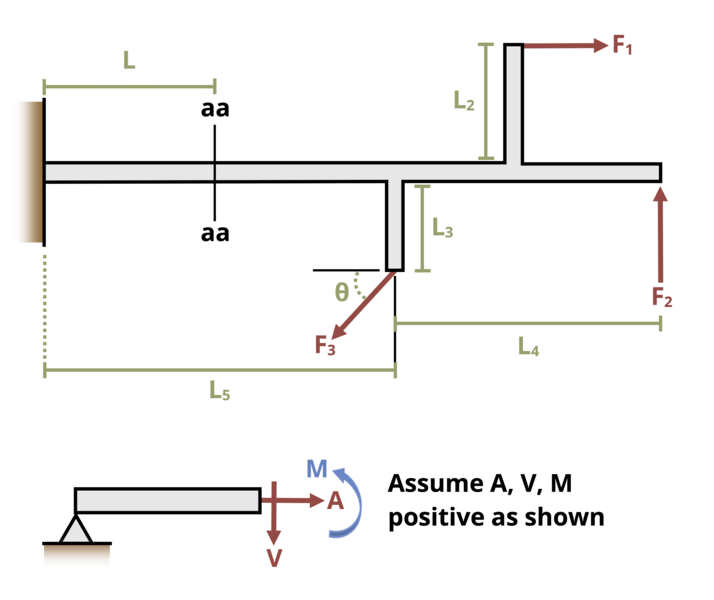
\includegraphics[keepaspectratio]{images/311.png}}
{[}Problem adapted from © Kurt Gramoll CC BY NC-SA 4.0{]}

\begin{Shaded}
\begin{Highlighting}[]
\NormalTok{\#| standalone: true}
\NormalTok{\#| viewerHeight: 600}
\NormalTok{\#| components: [viewer]}

\NormalTok{from shiny import App, render, ui, reactive}
\NormalTok{import random}
\NormalTok{import asyncio}
\NormalTok{import io}
\NormalTok{import math}
\NormalTok{import string}
\NormalTok{from datetime import datetime}
\NormalTok{from pathlib import Path}

\NormalTok{def generate\_random\_letters(length):}
\NormalTok{    \# Generate a random string of letters of specified length}
\NormalTok{    return \textquotesingle{}\textquotesingle{}.join(random.choice(string.ascii\_lowercase) for \_ in range(length))  }

\NormalTok{problem\_ID="312"}
\NormalTok{F1=reactive.Value("\_\_")}
\NormalTok{F2=reactive.Value("\_\_")}
\NormalTok{L1=reactive.Value("\_\_")}
\NormalTok{L2=reactive.Value("\_\_")}
  
\NormalTok{attempts=["Timestamp,Attempt,Answer,Feedback\textbackslash{}n"]}

\NormalTok{app\_ui = ui.page\_fluid(}
\NormalTok{    \#ui.markdown("**Please enter your ID number from your instructor and click to generate your problem**"),}
\NormalTok{    \#ui.input\_text("ID","", placeholder="Enter ID Number Here"),}
\NormalTok{    \#ui.input\_action\_button("generate\_problem", "Generate Problem", class\_="btn{-}primary"),}
\NormalTok{    ui.markdown("**Problem Statement**"),}
\NormalTok{    ui.output\_ui("ui\_problem\_statement"),}
\NormalTok{    ui.input\_text("answer","Your Answer in units of N{-}m", placeholder="Please enter your answer"),}
\NormalTok{    ui.input\_action\_button("submit", "Check Answer", class\_="btn{-}primary"),}
\NormalTok{    \#ui.download\_button("download", "Download File to Submit", class\_="btn{-}success"),}
\NormalTok{)}

\NormalTok{def server(input, output, session):}
\NormalTok{    \# Initialize a counter for attempts}
\NormalTok{    attempt\_counter = reactive.Value(0)}

\NormalTok{    @output}
\NormalTok{    @render.ui}
\NormalTok{    def ui\_problem\_statement():}
\NormalTok{        randomize\_vars()}
\NormalTok{        return[ui.markdown(f"A beam is loaded as shown, where loads F\textless{}sub\textgreater{}1\textless{}/sub\textgreater{} = \{F1()\} N, and F\textless{}sub\textgreater{}2\textless{}/sub\textgreater{} = \{F2()\} N. Lengths L\textless{}sub\textgreater{}1\textless{}/sub\textgreater{} = \{L1()\} mm and L\textless{}sub\textgreater{}2\textless{}/sub\textgreater{} = \{L2()\} mm. Determine the magnitude of the internal bending moment at section aa.")]}
    
\NormalTok{    \#@reactive.Effect}
\NormalTok{    \#@reactive.event(input.generate\_problem)}
\NormalTok{    def randomize\_vars():}
\NormalTok{        random.seed(101)}
\NormalTok{        F1.set(random.randrange(100,900,10))}
\NormalTok{        F2.set(random.randrange(100,900,10))}
\NormalTok{        L1.set(random.randrange(300,800,10))}
\NormalTok{        L2.set(L1()*2)}

\NormalTok{    @reactive.Effect}
\NormalTok{    @reactive.event(input.submit)}
\NormalTok{    def \_():}
\NormalTok{        attempt\_counter.set(attempt\_counter() + 1)  \# Increment the attempt counter on each submission.}
        
\NormalTok{        instr = {-}F1()*L1()/1000{-}F2()*L2()/1000*math.cos(45*math.pi/180)}
\NormalTok{        if math.isclose(float(input.answer()), instr, rel\_tol=0.01):}
\NormalTok{            check = "*Correct*"}
\NormalTok{            correct\_indicator = "JL"}
\NormalTok{        else:}
\NormalTok{            check = "*Not Correct.*"}
\NormalTok{            correct\_indicator = "JG"}

\NormalTok{        \# Generate random parts for the encoded attempt.}
\NormalTok{        random\_start = generate\_random\_letters(4)}
\NormalTok{        random\_middle = generate\_random\_letters(4)}
\NormalTok{        random\_end = generate\_random\_letters(4)}
\NormalTok{        \#encoded\_attempt = f"\{random\_start\}\{problem\_ID\}{-}\{random\_middle\}\{attempt\_counter()\}\{correct\_indicator\}{-}\{random\_end\}\{input.ID()\}"}

\NormalTok{        \# Store the most recent encoded attempt in a reactive value so it persists across submissions}
\NormalTok{        \#session.encoded\_attempt = reactive.Value(encoded\_attempt)}

\NormalTok{        \# Append the attempt data to the attempts list without the encoded attempt}
\NormalTok{        attempts.append(f"\{datetime.now()\}, \{attempt\_counter()\}, \{input.answer()\}, \{check\}\textbackslash{}n")}

\NormalTok{        \# Show feedback to the user.}
\NormalTok{        feedback = ui.markdown(f"Your answer of \{input.answer()\} is \{check\}.")}
\NormalTok{        m = ui.modal(}
\NormalTok{            feedback,}
\NormalTok{            title="Feedback",}
\NormalTok{            easy\_close=True}
\NormalTok{        )}
\NormalTok{        ui.modal\_show(m)}

\NormalTok{    \#@render.download(filename=lambda: f"Problem\_Log{-}\{problem\_ID\}{-}\{input.ID()\}.csv")}
\NormalTok{    async def download():}
\NormalTok{        \# Start the CSV with the encoded attempt (without label)}
\NormalTok{        final\_encoded = session.encoded\_attempt() if session.encoded\_attempt is not None else "No attempts"}
\NormalTok{        yield f"\{final\_encoded\}\textbackslash{}n\textbackslash{}n"}
        
\NormalTok{        \# Write the header for the remaining CSV data once}
\NormalTok{        yield "Timestamp,Attempt,Answer,Feedback\textbackslash{}n"}
        
\NormalTok{        \# Write the attempts data, ensure that the header from the attempts list is not written again}
\NormalTok{        for attempt in attempts[1:]:  \# Skip the first element which is the header}
\NormalTok{            await asyncio.sleep(0.25)  \# This delay may not be necessary; adjust as needed}
\NormalTok{            yield attempt}

\NormalTok{\# App installation}
\NormalTok{app = App(app\_ui, server)}
\end{Highlighting}
\end{Shaded}

\chapter*{Problem 7.6 - Internal Shear Force \& Bending Moments by
Equilibrium}\label{problem-7.6---internal-shear-force-bending-moments-by-equilibrium}
\addcontentsline{toc}{chapter}{Problem 7.6 - Internal Shear Force \&
Bending Moments by Equilibrium}

\markboth{Problem 7.6 - Internal Shear Force \& Bending Moments by
Equilibrium}{Problem 7.6 - Internal Shear Force \& Bending Moments by
Equilibrium}

\pandocbounded{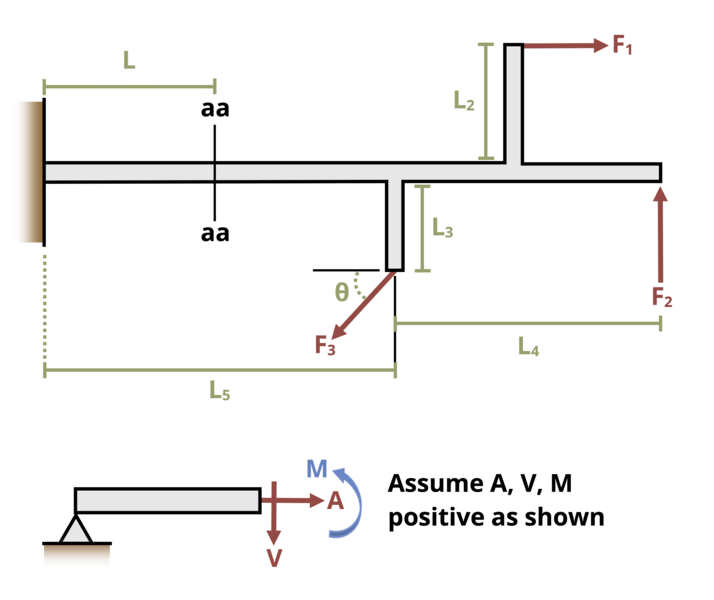
\includegraphics[keepaspectratio]{images/311.png}}
{[}Problem adapted from © Kurt Gramoll CC BY NC-SA 4.0{]}

\begin{Shaded}
\begin{Highlighting}[]
\NormalTok{\#| standalone: true}
\NormalTok{\#| viewerHeight: 600}
\NormalTok{\#| components: [viewer]}

\NormalTok{from shiny import App, render, ui, reactive}
\NormalTok{import random}
\NormalTok{import asyncio}
\NormalTok{import io}
\NormalTok{import math}
\NormalTok{import string}
\NormalTok{from datetime import datetime}
\NormalTok{from pathlib import Path}

\NormalTok{def generate\_random\_letters(length):}
\NormalTok{    \# Generate a random string of letters of specified length}
\NormalTok{    return \textquotesingle{}\textquotesingle{}.join(random.choice(string.ascii\_lowercase) for \_ in range(length))  }

\NormalTok{problem\_ID="313"}
\NormalTok{wo=reactive.Value("\_\_")}
\NormalTok{a=reactive.Value("\_\_")}
\NormalTok{b=reactive.Value("\_\_")}
  
\NormalTok{attempts=["Timestamp,Attempt,Answer,Feedback\textbackslash{}n"]}

\NormalTok{app\_ui = ui.page\_fluid(}
\NormalTok{    \#ui.markdown("**Please enter your ID number from your instructor and click to generate your problem**"),}
\NormalTok{    \#ui.input\_text("ID","", placeholder="Enter ID Number Here"),}
\NormalTok{    \#ui.input\_action\_button("generate\_problem", "Generate Problem", class\_="btn{-}primary"),}
\NormalTok{    ui.markdown("**Problem Statement**"),}
\NormalTok{    ui.output\_ui("ui\_problem\_statement"),}
\NormalTok{    ui.input\_text("answer","Your Answer in units of lb{-}in", placeholder="Please enter your answer"),}
\NormalTok{    ui.input\_action\_button("submit", "Check Answer", class\_="btn{-}primary"),}
\NormalTok{    \#ui.download\_button("download", "Download File to Submit", class\_="btn{-}success"),}
\NormalTok{)}

\NormalTok{def server(input, output, session):}
\NormalTok{    \# Initialize a counter for attempts}
\NormalTok{    attempt\_counter = reactive.Value(0)}

\NormalTok{    @output}
\NormalTok{    @render.ui}
\NormalTok{    def ui\_problem\_statement():}
\NormalTok{        randomize\_vars()}
\NormalTok{        return[ui.markdown(f"A beam with the profile shown is loaded with a linear distributed load as shown, where w\textless{}sub\textgreater{}0\textless{}/sub\textgreater{} = \{wo()\} lb/in. If distances a = \{a()\} in. and b = \{b()\} in., determine the internal bending moment at section aa.")]}
    
\NormalTok{    \#@reactive.Effect}
\NormalTok{    \#@reactive.event(input.generate\_problem)}
\NormalTok{    def randomize\_vars():}
\NormalTok{        random.seed(101)}
\NormalTok{        wo.set(random.randrange(100,1000,10))}
\NormalTok{        a.set(random.randrange(5,20,1))}
\NormalTok{        b.set(a(){-}random.randrange(1,2,1))}

\NormalTok{    @reactive.Effect}
\NormalTok{    @reactive.event(input.submit)}
\NormalTok{    def \_():}
\NormalTok{        attempt\_counter.set(attempt\_counter() + 1)  \# Increment the attempt counter on each submission.}
        
\NormalTok{        instr = 0.5*wo()*2*b()*b()/3}
\NormalTok{        if math.isclose(float(input.answer()), instr, rel\_tol=0.01):}
\NormalTok{            check = "*Correct*"}
\NormalTok{            correct\_indicator = "JL"}
\NormalTok{        else:}
\NormalTok{            check = "*Not Correct.*"}
\NormalTok{            correct\_indicator = "JG"}

\NormalTok{        \# Generate random parts for the encoded attempt.}
\NormalTok{        random\_start = generate\_random\_letters(4)}
\NormalTok{        random\_middle = generate\_random\_letters(4)}
\NormalTok{        random\_end = generate\_random\_letters(4)}
\NormalTok{        \#encoded\_attempt = f"\{random\_start\}\{problem\_ID\}{-}\{random\_middle\}\{attempt\_counter()\}\{correct\_indicator\}{-}\{random\_end\}\{input.ID()\}"}

\NormalTok{        \# Store the most recent encoded attempt in a reactive value so it persists across submissions}
\NormalTok{        \#session.encoded\_attempt = reactive.Value(encoded\_attempt)}

\NormalTok{        \# Append the attempt data to the attempts list without the encoded attempt}
\NormalTok{        attempts.append(f"\{datetime.now()\}, \{attempt\_counter()\}, \{input.answer()\}, \{check\}\textbackslash{}n")}

\NormalTok{        \# Show feedback to the user.}
\NormalTok{        feedback = ui.markdown(f"Your answer of \{input.answer()\} is \{check\}.")}
\NormalTok{        m = ui.modal(}
\NormalTok{            feedback,}
\NormalTok{            title="Feedback",}
\NormalTok{            easy\_close=True}
\NormalTok{        )}
\NormalTok{        ui.modal\_show(m)}

\NormalTok{    \#@render.download(filename=lambda: f"Problem\_Log{-}\{problem\_ID\}{-}\{input.ID()\}.csv")}
\NormalTok{    async def download():}
\NormalTok{        \# Start the CSV with the encoded attempt (without label)}
\NormalTok{        final\_encoded = session.encoded\_attempt() if session.encoded\_attempt is not None else "No attempts"}
\NormalTok{        yield f"\{final\_encoded\}\textbackslash{}n\textbackslash{}n"}
        
\NormalTok{        \# Write the header for the remaining CSV data once}
\NormalTok{        yield "Timestamp,Attempt,Answer,Feedback\textbackslash{}n"}
        
\NormalTok{        \# Write the attempts data, ensure that the header from the attempts list is not written again}
\NormalTok{        for attempt in attempts[1:]:  \# Skip the first element which is the header}
\NormalTok{            await asyncio.sleep(0.25)  \# This delay may not be necessary; adjust as needed}
\NormalTok{            yield attempt}

\NormalTok{\# App installation}
\NormalTok{app = App(app\_ui, server)}
\end{Highlighting}
\end{Shaded}

\chapter*{Problem 7.7 - Internal Shear Force \& Bending Moments by
Equilibrium}\label{problem-7.7---internal-shear-force-bending-moments-by-equilibrium}
\addcontentsline{toc}{chapter}{Problem 7.7 - Internal Shear Force \&
Bending Moments by Equilibrium}

\markboth{Problem 7.7 - Internal Shear Force \& Bending Moments by
Equilibrium}{Problem 7.7 - Internal Shear Force \& Bending Moments by
Equilibrium}

\pandocbounded{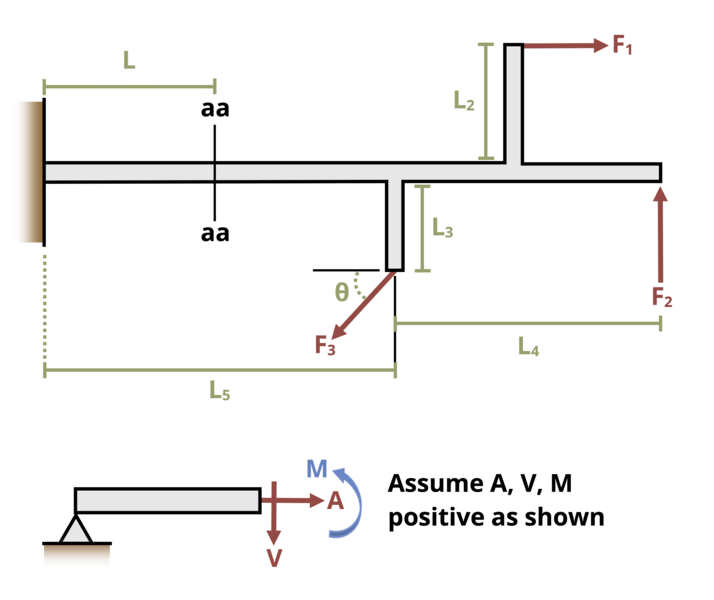
\includegraphics[keepaspectratio]{images/311.png}}
{[}Problem adapted from © Kurt Gramoll CC BY NC-SA 4.0{]}

\begin{Shaded}
\begin{Highlighting}[]
\NormalTok{\#| standalone: true}
\NormalTok{\#| viewerHeight: 600}
\NormalTok{\#| components: [viewer]}

\NormalTok{from shiny import App, render, ui, reactive}
\NormalTok{import random}
\NormalTok{import asyncio}
\NormalTok{import io}
\NormalTok{import math}
\NormalTok{import string}
\NormalTok{from datetime import datetime}
\NormalTok{from pathlib import Path}

\NormalTok{def generate\_random\_letters(length):}
\NormalTok{    \# Generate a random string of letters of specified length}
\NormalTok{    return \textquotesingle{}\textquotesingle{}.join(random.choice(string.ascii\_lowercase) for \_ in range(length))  }

\NormalTok{problem\_ID="316"}
\NormalTok{r=reactive.Value("\_\_")}
\NormalTok{L=reactive.Value("\_\_")}
\NormalTok{w=reactive.Value("\_\_")}
  
\NormalTok{attempts=["Timestamp,Attempt,Answer,Feedback\textbackslash{}n"]}

\NormalTok{app\_ui = ui.page\_fluid(}
\NormalTok{    \#ui.markdown("**Please enter your ID number from your instructor and click to generate your problem**"),}
\NormalTok{    \#ui.input\_text("ID","", placeholder="Enter ID Number Here"),}
\NormalTok{    \#ui.input\_action\_button("generate\_problem", "Generate Problem", class\_="btn{-}primary"),}
\NormalTok{    ui.markdown("**Problem Statement**"),}
\NormalTok{    ui.output\_ui("ui\_problem\_statement"),}
\NormalTok{    ui.input\_text("answer","Your Answer in units of kN{-}m", placeholder="Please enter your answer"),}
\NormalTok{    ui.input\_action\_button("submit", "Check Answer", class\_="btn{-}primary"),}
\NormalTok{    \#ui.download\_button("download", "Download File to Submit", class\_="btn{-}success"),}
\NormalTok{)}

\NormalTok{def server(input, output, session):}
\NormalTok{    \# Initialize a counter for attempts}
\NormalTok{    attempt\_counter = reactive.Value(0)}

\NormalTok{    @output}
\NormalTok{    @render.ui}
\NormalTok{    def ui\_problem\_statement():}
\NormalTok{        randomize\_vars()}
\NormalTok{        return[ui.markdown(f"A beam is loaded as shown, where radius r = \{r()\} m, length L = \{L()\} m, and distributed load w = \{w()\} kN/m. Determine the internal bending moment at section aa (half way between B and C).")]}
    
\NormalTok{    \#@reactive.Effect}
\NormalTok{    \#@reactive.event(input.generate\_problem)}
\NormalTok{    def randomize\_vars():}
\NormalTok{        random.seed(101)}
\NormalTok{        r.set(random.randrange(5,20,1)/10)}
\NormalTok{        L.set(round(r())*random.randrange(10,20,1)/10)}
\NormalTok{        w.set(random.randrange(1,30,1))}

\NormalTok{    @reactive.Effect}
\NormalTok{    @reactive.event(input.submit)}
\NormalTok{    def \_():}
\NormalTok{        attempt\_counter.set(attempt\_counter() + 1)  \# Increment the attempt counter on each submission.}
\NormalTok{        Cy = w()*L()/2}
\NormalTok{        instr = Cy*L()/2{-}w()*L()/2*L()/4}
\NormalTok{        if math.isclose(float(input.answer()), instr, rel\_tol=0.01):}
\NormalTok{            check = "*Correct*"}
\NormalTok{            correct\_indicator = "JL"}
\NormalTok{        else:}
\NormalTok{            check = "*Not Correct.*"}
\NormalTok{            correct\_indicator = "JG"}

\NormalTok{        \# Generate random parts for the encoded attempt.}
\NormalTok{        random\_start = generate\_random\_letters(4)}
\NormalTok{        random\_middle = generate\_random\_letters(4)}
\NormalTok{        random\_end = generate\_random\_letters(4)}
\NormalTok{        \#encoded\_attempt = f"\{random\_start\}\{problem\_ID\}{-}\{random\_middle\}\{attempt\_counter()\}\{correct\_indicator\}{-}\{random\_end\}\{input.ID()\}"}

\NormalTok{        \# Store the most recent encoded attempt in a reactive value so it persists across submissions}
\NormalTok{        \#session.encoded\_attempt = reactive.Value(encoded\_attempt)}

\NormalTok{        \# Append the attempt data to the attempts list without the encoded attempt}
\NormalTok{        attempts.append(f"\{datetime.now()\}, \{attempt\_counter()\}, \{input.answer()\}, \{check\}\textbackslash{}n")}

\NormalTok{        \# Show feedback to the user.}
\NormalTok{        feedback = ui.markdown(f"Your answer of \{input.answer()\} is \{check\}.")}
\NormalTok{        m = ui.modal(}
\NormalTok{            feedback,}
\NormalTok{            title="Feedback",}
\NormalTok{            easy\_close=True}
\NormalTok{        )}
\NormalTok{        ui.modal\_show(m)}

\NormalTok{    \#@render.download(filename=lambda: f"Problem\_Log{-}\{problem\_ID\}{-}\{input.ID()\}.csv")}
\NormalTok{    async def download():}
\NormalTok{        \# Start the CSV with the encoded attempt (without label)}
\NormalTok{        final\_encoded = session.encoded\_attempt() if session.encoded\_attempt is not None else "No attempts"}
\NormalTok{        yield f"\{final\_encoded\}\textbackslash{}n\textbackslash{}n"}
        
\NormalTok{        \# Write the header for the remaining CSV data once}
\NormalTok{        yield "Timestamp,Attempt,Answer,Feedback\textbackslash{}n"}
        
\NormalTok{        \# Write the attempts data, ensure that the header from the attempts list is not written again}
\NormalTok{        for attempt in attempts[1:]:  \# Skip the first element which is the header}
\NormalTok{            await asyncio.sleep(0.25)  \# This delay may not be necessary; adjust as needed}
\NormalTok{            yield attempt}

\NormalTok{\# App installation}
\NormalTok{app = App(app\_ui, server)}
\end{Highlighting}
\end{Shaded}

\chapter*{Problem 7.8 - Internal Shear Force \& Bending Moments by
Equilibrium}\label{problem-7.8---internal-shear-force-bending-moments-by-equilibrium}
\addcontentsline{toc}{chapter}{Problem 7.8 - Internal Shear Force \&
Bending Moments by Equilibrium}

\markboth{Problem 7.8 - Internal Shear Force \& Bending Moments by
Equilibrium}{Problem 7.8 - Internal Shear Force \& Bending Moments by
Equilibrium}

\pandocbounded{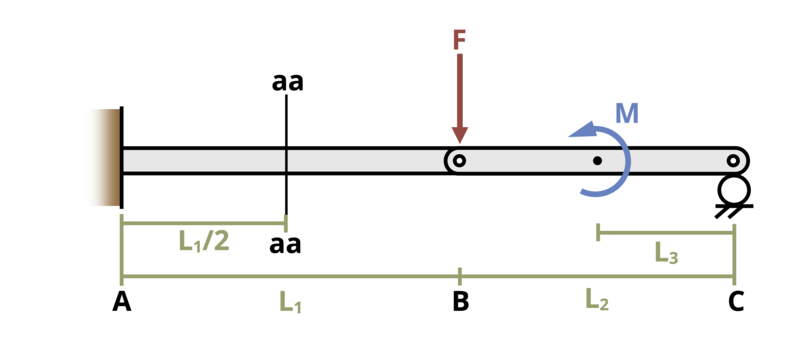
\includegraphics[keepaspectratio]{images/317.png}}
{[}Problem adapted from © Kurt Gramoll CC BY NC-SA 4.0{]}

\begin{Shaded}
\begin{Highlighting}[]
\NormalTok{\#| standalone: true}
\NormalTok{\#| viewerHeight: 600}
\NormalTok{\#| components: [viewer]}

\NormalTok{from shiny import App, render, ui, reactive}
\NormalTok{import random}
\NormalTok{import asyncio}
\NormalTok{import io}
\NormalTok{import math}
\NormalTok{import string}
\NormalTok{from datetime import datetime}
\NormalTok{from pathlib import Path}

\NormalTok{def generate\_random\_letters(length):}
\NormalTok{    \# Generate a random string of letters of specified length}
\NormalTok{    return \textquotesingle{}\textquotesingle{}.join(random.choice(string.ascii\_lowercase) for \_ in range(length))  }

\NormalTok{problem\_ID="317"}
\NormalTok{F=reactive.Value("\_\_")}
\NormalTok{M=reactive.Value("\_\_")}
\NormalTok{L1=reactive.Value("\_\_")}
\NormalTok{L2=reactive.Value("\_\_")}
\NormalTok{L3=reactive.Value("\_\_")}
  
\NormalTok{attempts=["Timestamp,Attempt,Answer,Feedback\textbackslash{}n"]}

\NormalTok{app\_ui = ui.page\_fluid(}
\NormalTok{    \#ui.markdown("**Please enter your ID number from your instructor and click to generate your problem**"),}
\NormalTok{    \#ui.input\_text("ID","", placeholder="Enter ID Number Here"),}
\NormalTok{    \#ui.input\_action\_button("generate\_problem", "Generate Problem", class\_="btn{-}primary"),}
\NormalTok{    ui.markdown("**Problem Statement**"),}
\NormalTok{    ui.output\_ui("ui\_problem\_statement"),}
\NormalTok{    ui.input\_text("answer","Your Answer in units of kN{-}m", placeholder="Please enter your answer"),}
\NormalTok{    ui.input\_action\_button("submit", "Check Answer", class\_="btn{-}primary"),}
\NormalTok{    \#ui.download\_button("download", "Download File to Submit", class\_="btn{-}success"),}
\NormalTok{)}

\NormalTok{def server(input, output, session):}
\NormalTok{    \# Initialize a counter for attempts}
\NormalTok{    attempt\_counter = reactive.Value(0)}

\NormalTok{    @output}
\NormalTok{    @render.ui}
\NormalTok{    def ui\_problem\_statement():}
\NormalTok{        randomize\_vars()}
\NormalTok{        return[ui.markdown(f"A beam is loaded as shown, where loads F = \{F()\} kN, and M = \{M()\} kN{-}m. If lengths L\textless{}sub\textgreater{}1\textless{}/sub\textgreater{} = \{L1()\} m, L\textless{}sub\textgreater{}2\textless{}/sub\textgreater{} = \{L2()\} m, and L\textless{}sub\textgreater{}3\textless{}/sub\textgreater{} = \{L3()\} m, determine the magnitude of the internal bending moment at section aa (half way between points A and B).")]}
    
\NormalTok{    \#@reactive.Effect}
\NormalTok{    \#@reactive.event(input.generate\_problem)}
\NormalTok{    def randomize\_vars():}
\NormalTok{        random.seed(101)}
\NormalTok{        F.set(random.randrange(1,20,1))}
\NormalTok{        M.set(random.randrange(1,20,1))}
\NormalTok{        L1.set(random.randrange(10,20,1)/10)}
\NormalTok{        L2.set(L1()*2)}
\NormalTok{        L3.set(L2()+random.randrange(5,15,1)/10)}

\NormalTok{    @reactive.Effect}
\NormalTok{    @reactive.event(input.submit)}
\NormalTok{    def \_():}
\NormalTok{        attempt\_counter.set(attempt\_counter() + 1)  \# Increment the attempt counter on each submission.}
\NormalTok{        Cy = {-}M()/L2()}
\NormalTok{        By = Cy+F()}
\NormalTok{        instr = {-}By*L1()/2}
\NormalTok{        if math.isclose(float(input.answer()), instr, rel\_tol=0.01):}
\NormalTok{            check = "*Correct*"}
\NormalTok{            correct\_indicator = "JL"}
\NormalTok{        else:}
\NormalTok{            check = "*Not Correct.*"}
\NormalTok{            correct\_indicator = "JG"}

\NormalTok{        \# Generate random parts for the encoded attempt.}
\NormalTok{        random\_start = generate\_random\_letters(4)}
\NormalTok{        random\_middle = generate\_random\_letters(4)}
\NormalTok{        random\_end = generate\_random\_letters(4)}
\NormalTok{        \#encoded\_attempt = f"\{random\_start\}\{problem\_ID\}{-}\{random\_middle\}\{attempt\_counter()\}\{correct\_indicator\}{-}\{random\_end\}\{input.ID()\}"}

\NormalTok{        \# Store the most recent encoded attempt in a reactive value so it persists across submissions}
\NormalTok{        \#session.encoded\_attempt = reactive.Value(encoded\_attempt)}

\NormalTok{        \# Append the attempt data to the attempts list without the encoded attempt}
\NormalTok{        attempts.append(f"\{datetime.now()\}, \{attempt\_counter()\}, \{input.answer()\}, \{check\}\textbackslash{}n")}

\NormalTok{        \# Show feedback to the user.}
\NormalTok{        feedback = ui.markdown(f"Your answer of \{input.answer()\} is \{check\}.")}
\NormalTok{        m = ui.modal(}
\NormalTok{            feedback,}
\NormalTok{            title="Feedback",}
\NormalTok{            easy\_close=True}
\NormalTok{        )}
\NormalTok{        ui.modal\_show(m)}

\NormalTok{    \#@render.download(filename=lambda: f"Problem\_Log{-}\{problem\_ID\}{-}\{input.ID()\}.csv")}
\NormalTok{    async def download():}
\NormalTok{        \# Start the CSV with the encoded attempt (without label)}
\NormalTok{        final\_encoded = session.encoded\_attempt() if session.encoded\_attempt is not None else "No attempts"}
\NormalTok{        yield f"\{final\_encoded\}\textbackslash{}n\textbackslash{}n"}
        
\NormalTok{        \# Write the header for the remaining CSV data once}
\NormalTok{        yield "Timestamp,Attempt,Answer,Feedback\textbackslash{}n"}
        
\NormalTok{        \# Write the attempts data, ensure that the header from the attempts list is not written again}
\NormalTok{        for attempt in attempts[1:]:  \# Skip the first element which is the header}
\NormalTok{            await asyncio.sleep(0.25)  \# This delay may not be necessary; adjust as needed}
\NormalTok{            yield attempt}

\NormalTok{\# App installation}
\NormalTok{app = App(app\_ui, server)}
\end{Highlighting}
\end{Shaded}

\chapter*{Problem 7.14 - Shear Force \& Bending Moment
Equations}\label{problem-7.14---shear-force-bending-moment-equations}
\addcontentsline{toc}{chapter}{Problem 7.14 - Shear Force \& Bending
Moment Equations}

\markboth{Problem 7.14 - Shear Force \& Bending Moment
Equations}{Problem 7.14 - Shear Force \& Bending Moment Equations}

\pandocbounded{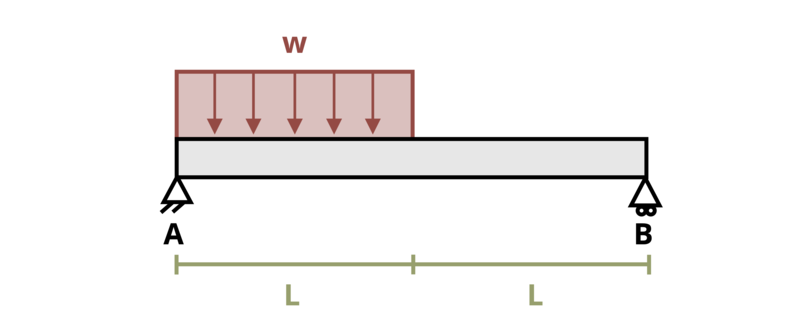
\includegraphics[keepaspectratio]{images/318.png}}
{[}Problem adapted from © Kurt Gramoll CC BY NC-SA 4.0{]}

\begin{Shaded}
\begin{Highlighting}[]
\NormalTok{\#| standalone: true}
\NormalTok{\#| viewerHeight: 600}
\NormalTok{\#| components: [viewer]}

\NormalTok{from shiny import App, render, ui, reactive}
\NormalTok{import random}
\NormalTok{import asyncio}
\NormalTok{import io}
\NormalTok{import math}
\NormalTok{import string}
\NormalTok{from datetime import datetime}
\NormalTok{from pathlib import Path}

\NormalTok{def generate\_random\_letters(length):}
\NormalTok{    return \textquotesingle{}\textquotesingle{}.join(random.choice(string.ascii\_lowercase) for \_ in range(length))}

\NormalTok{problem\_ID = "318"}
\NormalTok{w = reactive.Value("\_\_")}
\NormalTok{L = reactive.Value("\_\_")}

\NormalTok{attempts = ["Timestamp,Attempt,Answer1,Answer2,Feedback\textbackslash{}n"]}

\NormalTok{app\_ui = ui.page\_fluid(}
\NormalTok{    \#ui.markdown("**Please enter your ID number from your instructor and click to generate your problem**"),}
\NormalTok{    \#ui.input\_text("ID", "", placeholder="Enter ID Number Here"),}
\NormalTok{    \#ui.input\_action\_button("generate\_problem", "Generate Problem", class\_="btn{-}primary"),}
\NormalTok{    ui.markdown("**Problem Statement**"),}
\NormalTok{    ui.output\_ui("ui\_problem\_statement"),}
\NormalTok{    ui.input\_text("answer1", "Your internal shear force answer in units of kip", placeholder="Please enter your answer 1"),}
\NormalTok{    ui.input\_text("answer2", "Your moment answer in units of kip{-}ft", placeholder="Please enter your answer 2"),}
\NormalTok{    ui.input\_action\_button("submit", "Check Answers", class\_="btn{-}primary"),}
\NormalTok{    \#ui.download\_button("download", "Download File to Submit", class\_="btn{-}success"),}
\NormalTok{)}

\NormalTok{def server(input, output, session):}
\NormalTok{    attempt\_counter = reactive.Value(0)}

\NormalTok{    @output}
\NormalTok{    @render.ui}
\NormalTok{    def ui\_problem\_statement():}
\NormalTok{        randomize\_vars()}
\NormalTok{        return [ui.markdown(f"Plot the shear force and bending moment diagrams for the loading shown. Assume w = \{w()\} kip/ft and L = \{L()\} ft. What is the maximum absolute shear force and maximum absolute bending moment?")]}

\NormalTok{    \#@reactive.Effect}
\NormalTok{    \#@reactive.event(input.generate\_problem)}
\NormalTok{    def randomize\_vars():}
\NormalTok{        random.seed(101)}
\NormalTok{        w.set(random.randrange(30, 200, 1)/10)}
\NormalTok{        L.set(random.randrange(40, 100, 1)/10)}

\NormalTok{    @reactive.Effect}
\NormalTok{    @reactive.event(input.submit)}
\NormalTok{    def \_():}
\NormalTok{        attempt\_counter.set(attempt\_counter() + 1)}
\NormalTok{        instr1 = 3/4*w()*L()}
\NormalTok{        instr2 = instr1**2/(2*w())}
\NormalTok{        correct1 = math.isclose(float(input.answer1()), instr1, rel\_tol=0.01)}
\NormalTok{        correct2 = math.isclose(float(input.answer2()), instr2, rel\_tol=0.01)}
        
\NormalTok{        if correct1 and correct2:}
\NormalTok{            check = "both correct."}
\NormalTok{        elif correct1:}
\NormalTok{            check = f" \{\textquotesingle{}correct for answer 1 and incorrect for answer 2.\textquotesingle{}\}"}
\NormalTok{        elif correct2:}
\NormalTok{            check = f"\{\textquotesingle{}incorrect for answer 1 and correct for answer 2.\textquotesingle{}\}"}
\NormalTok{        else:}
\NormalTok{            check = f"\{\textquotesingle{}both incorrect.\textquotesingle{}\}"}
            
\NormalTok{        correct\_indicator = "JL" if correct1 and correct2 else "JG"}

\NormalTok{        random\_start = generate\_random\_letters(4)}
\NormalTok{        random\_middle = generate\_random\_letters(4)}
\NormalTok{        random\_end = generate\_random\_letters(4)}
\NormalTok{        \#encoded\_attempt = f"\{random\_start\}\{problem\_ID\}{-}\{random\_middle\}\{attempt\_counter()\}\{correct\_indicator\}{-}\{random\_end\}\{input.ID()\}"}

\NormalTok{        \#session.encoded\_attempt = reactive.Value(encoded\_attempt)}
\NormalTok{        attempts.append(f"\{datetime.now()\}, \{attempt\_counter()\}, \{input.answer1()\}, \{input.answer2()\}, \{check\}\textbackslash{}n")}

\NormalTok{        feedback = ui.markdown(f"Your answers of \{input.answer1()\} and \{input.answer2()\} are \{check\}.")}
\NormalTok{        m = ui.modal(feedback, title="Feedback", easy\_close=True)}
\NormalTok{        ui.modal\_show(m)}

\NormalTok{    \#@render.download(filename=lambda: f"Problem\_Log{-}\{problem\_ID\}{-}\{input.ID()\}.csv")}
\NormalTok{    async def download():}
\NormalTok{        final\_encoded = session.encoded\_attempt() if session.encoded\_attempt is not None else "No attempts"}
\NormalTok{        yield f"\{final\_encoded\}\textbackslash{}n\textbackslash{}n"}
\NormalTok{        yield "Timestamp,Attempt,Answer1,Answer2,Feedback\textbackslash{}n"}
\NormalTok{        for attempt in attempts[1:]:}
\NormalTok{            await asyncio.sleep(0.25)}
\NormalTok{            yield attempt}

\NormalTok{app = App(app\_ui, server)}
\end{Highlighting}
\end{Shaded}

\chapter*{Problem 7.15 - Shear Force \& Bending Moment
Equations}\label{problem-7.15---shear-force-bending-moment-equations}
\addcontentsline{toc}{chapter}{Problem 7.15 - Shear Force \& Bending
Moment Equations}

\markboth{Problem 7.15 - Shear Force \& Bending Moment
Equations}{Problem 7.15 - Shear Force \& Bending Moment Equations}

\pandocbounded{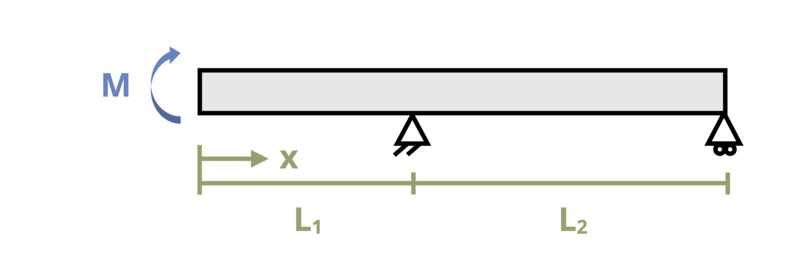
\includegraphics[keepaspectratio]{images/320.png}}
{[}Problem adapted from © Kurt Gramoll CC BY NC-SA 4.0{]}

\begin{Shaded}
\begin{Highlighting}[]
\NormalTok{\#| standalone: true}
\NormalTok{\#| viewerHeight: 600}
\NormalTok{\#| components: [viewer]}
\NormalTok{from shiny import App, render, ui, reactive}
\NormalTok{import random}
\NormalTok{import asyncio}
\NormalTok{import io}
\NormalTok{import math}
\NormalTok{import string}
\NormalTok{from datetime import datetime}
\NormalTok{from pathlib import Path}

\NormalTok{def generate\_random\_letters(length):}
\NormalTok{    \# Generate a random string of letters of specified length}
\NormalTok{    return \textquotesingle{}\textquotesingle{}.join(random.choice(string.ascii\_lowercase) for \_ in range(length))}

\NormalTok{problem\_ID="320"}
\NormalTok{M=reactive.Value("\_\_")}
\NormalTok{L1=reactive.Value("\_\_")}
\NormalTok{L2=reactive.Value("\_\_")}
\NormalTok{attempts=["Timestamp,Attempt,Answer,Feedback\textbackslash{}n"]}

\NormalTok{app\_ui = ui.page\_fluid(}
\NormalTok{    \#ui.markdown("**Please enter your ID number from your instructor and click to generate your problem**"),}
\NormalTok{    \#ui.input\_text("ID","", placeholder="Enter ID Number Here"),}
\NormalTok{    \#ui.input\_action\_button("generate\_problem", "Generate Problem", class\_="btn{-}primary"),}
\NormalTok{    ui.markdown("**Problem Statement**"),}
\NormalTok{    ui.output\_ui("ui\_problem\_statement"),}
\NormalTok{    ui.input\_text("answer1","Maximum absolute shear force in units of kip", placeholder="Please enter your answer 1"),}
\NormalTok{    ui.input\_text("answer2","Maximum absolute bending moment in units of kip{-}ft", placeholder="Please enter your answer 2"),}
\NormalTok{    ui.input\_action\_button("submit", "Check Answers", class\_="btn{-}primary"),}
\NormalTok{    \#ui.download\_button("download", "Download File to Submit", class\_="btn{-}success"),}
\NormalTok{)}

\NormalTok{def server(input, output, session):}
\NormalTok{    \# Initialize a counter for attempts}
\NormalTok{    attempt\_counter = reactive.Value(0)}
    
\NormalTok{    @output}
\NormalTok{    @render.ui}
\NormalTok{    def ui\_problem\_statement():}
\NormalTok{        randomize\_vars()}
\NormalTok{        return[ui.markdown(f"Plot the shear force and bending moment diagrams for the loading shown. Assume M = \{M()\} kip{-}ft, L\textless{}sub\textgreater{}1\textless{}/sub\textgreater{} = \{L1()\} ft, and L\textless{}sub\textgreater{}2\textless{}/sub\textgreater{} = \{L2()\} ft. What is the maximum absolute shear force and maximum absolute bending moment? ")]}
    
\NormalTok{    \#@reactive.Effect}
\NormalTok{    \#@reactive.event(input.generate\_problem)}
\NormalTok{    def randomize\_vars():}
\NormalTok{        random.seed(101)}
\NormalTok{        M.set(random.randrange(5, 80, 1))}
\NormalTok{        L1.set(random.randrange(30, 100, 1)/10)}
\NormalTok{        L2.set(round(L1()*4/3,1))}
\NormalTok{    @reactive.Effect}
\NormalTok{    @reactive.event(input.submit)}
\NormalTok{    def \_():}
\NormalTok{        attempt\_counter.set(attempt\_counter() + 1)}
\NormalTok{        instr1= abs(M()/L2())}
\NormalTok{        instr2 = M()}
\NormalTok{        correct1 = math.isclose(float(input.answer1()), instr1, rel\_tol=0.01)}
\NormalTok{        correct2 = math.isclose(float(input.answer2()), instr2, rel\_tol=0.01)}
        
\NormalTok{        if correct1 and correct2:}
\NormalTok{            check = "both correct."}
\NormalTok{        else:}
\NormalTok{            check = f" \{\textquotesingle{}correct\textquotesingle{} if correct1 else \textquotesingle{}incorrect\textquotesingle{}\} and \{\textquotesingle{}correct respectively\textquotesingle{} if correct2 else \textquotesingle{}incorrect respectively\textquotesingle{}\}."}
        
\NormalTok{        correct\_indicator = "JL" if correct1 and correct2 else "JG"}

\NormalTok{        \# Generate random parts for the encoded attempt.}
\NormalTok{        random\_start = generate\_random\_letters(4)}
\NormalTok{        random\_middle = generate\_random\_letters(4)}
\NormalTok{        random\_end = generate\_random\_letters(4)}
\NormalTok{        \#encoded\_attempt = f"\{random\_start\}\{problem\_ID\}{-}\{random\_middle\}\{attempt\_counter()\}\{correct\_indicator\}{-}\{random\_end\}\{input.ID()\}"}

\NormalTok{        \# Store the most recent encoded attempt in a reactive value so it persists across submissions}
\NormalTok{        \#session.encoded\_attempt = reactive.Value(encoded\_attempt)}

\NormalTok{        \# Append the attempt data to the attempts list without the encoded attempt}
\NormalTok{        attempts.append(f"\{datetime.now()\}, \{attempt\_counter()\}, \{input.answer1()\}, \{input.answer2()\}, \{check\}\textbackslash{}n")}

\NormalTok{        \# Show feedback to the user.}
\NormalTok{        feedback = ui.markdown(f"Your answers of \{input.answer1()\} and \{input.answer2()\} are \{check\}.")}
\NormalTok{        m = ui.modal(feedback, title="Feedback", easy\_close=True)}
\NormalTok{        ui.modal\_show(m)}

\NormalTok{    \#@render.download(filename=lambda: f"Problem\_Log{-}\{problem\_ID\}{-}\{input.ID()\}.csv")}
\NormalTok{    async def download():}
\NormalTok{        \# Start the CSV with the encoded attempt (without label)}
\NormalTok{        final\_encoded = session.encoded\_attempt() if session.encoded\_attempt is not None else "No attempts"}
\NormalTok{        yield f"\{final\_encoded\}\textbackslash{}n\textbackslash{}n"}
        
\NormalTok{        \# Write the header for the remaining CSV data once}
\NormalTok{        yield "Timestamp,Attempt,Answer,Feedback\textbackslash{}n"}
        
\NormalTok{        \# Write the attempts data, ensure that the header from the attempts list is not written again}
\NormalTok{        for attempt in attempts[1:]:  \# Skip the first element which is the header}
\NormalTok{            await asyncio.sleep(0.25)  \# This delay may not be necessary; adjust as needed}
\NormalTok{            yield attempt}
            
\NormalTok{app = App(app\_ui, server)}
\end{Highlighting}
\end{Shaded}

\chapter*{Problem 7.16 - Shear Force \& Bending Moment
Equations}\label{problem-7.16---shear-force-bending-moment-equations}
\addcontentsline{toc}{chapter}{Problem 7.16 - Shear Force \& Bending
Moment Equations}

\markboth{Problem 7.16 - Shear Force \& Bending Moment
Equations}{Problem 7.16 - Shear Force \& Bending Moment Equations}

\pandocbounded{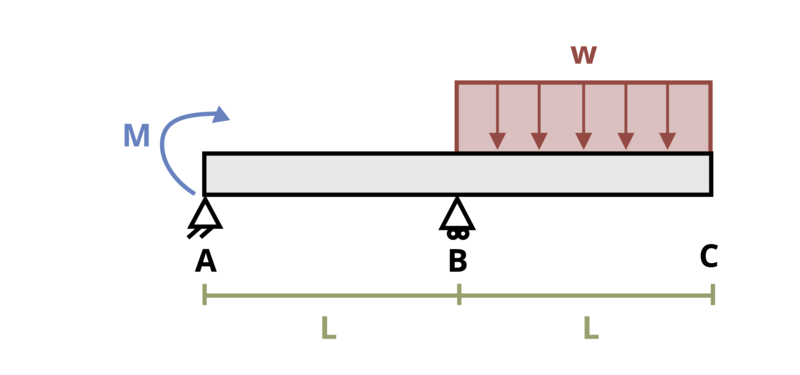
\includegraphics[keepaspectratio]{images/322.png}}
{[}Problem adapted from © Kurt Gramoll CC BY NC-SA 4.0{]}

\begin{Shaded}
\begin{Highlighting}[]
\NormalTok{\#| standalone: true}
\NormalTok{\#| viewerHeight: 600}
\NormalTok{\#| components: [viewer]}
\NormalTok{from shiny import App, render, ui, reactive}
\NormalTok{import random}
\NormalTok{import asyncio}
\NormalTok{import io}
\NormalTok{import math}
\NormalTok{import string}
\NormalTok{from datetime import datetime}
\NormalTok{from pathlib import Path}

\NormalTok{def generate\_random\_letters(length):}
\NormalTok{    \# Generate a random string of letters of specified length}
\NormalTok{    return \textquotesingle{}\textquotesingle{}.join(random.choice(string.ascii\_lowercase) for \_ in range(length))}

\NormalTok{problem\_ID="322"}
\NormalTok{w=reactive.Value("\_\_")}
\NormalTok{M=reactive.Value("\_\_")}
\NormalTok{L=reactive.Value("\_\_")}
\NormalTok{attempts=["Timestamp,Attempt,Answer,Feedback\textbackslash{}n"]}

\NormalTok{app\_ui = ui.page\_fluid(}
\NormalTok{    \#ui.markdown("**Please enter your ID number from your instructor and click to generate your problem**"),}
\NormalTok{    \#ui.input\_text("ID","", placeholder="Enter ID Number Here"),}
\NormalTok{    \#ui.input\_action\_button("generate\_problem", "Generate Problem", class\_="btn{-}primary"),}
\NormalTok{    ui.markdown("**Problem Statement**"),}
\NormalTok{    ui.output\_ui("ui\_problem\_statement"),}
\NormalTok{    ui.input\_text("answer1","Maximum absolute shear force in units of lb", placeholder="Please enter your answer 1"),}
\NormalTok{    ui.input\_text("answer2","Maximum absolute bending moment in units of lb{-}ft", placeholder="Please enter your answer 2"),}
\NormalTok{    ui.input\_action\_button("submit", "Check Answers", class\_="btn{-}primary"),}
\NormalTok{    \#ui.download\_button("download", "Download File to Submit", class\_="btn{-}success"),}
\NormalTok{)}

\NormalTok{def server(input, output, session):}
\NormalTok{    \# Initialize a counter for attempts}
\NormalTok{    attempt\_counter = reactive.Value(0)}
    
\NormalTok{    @output}
\NormalTok{    @render.ui}
\NormalTok{    def ui\_problem\_statement():}
\NormalTok{        randomize\_vars()}
\NormalTok{        return[ui.markdown(f"Plot the shear force and bending moment diagrams for the loading shown. Assume w = \{w()\} lb/ft, M = \{M()\} lb{-}ft, and L = \{L()\} ft. What is the maximum absolute shear force and maximum absolute bending moment? ")]}
    
\NormalTok{    \#@reactive.Effect}
\NormalTok{    \#@reactive.event(input.generate\_problem)}
\NormalTok{    def randomize\_vars():}
\NormalTok{        random.seed(101)}
\NormalTok{        w.set(random.randrange(10, 100, 1))}
\NormalTok{        M.set(random.randrange(100, 3300, 10))}
\NormalTok{        L.set(random.randrange(5, 15, 1))}
\NormalTok{    @reactive.Effect}
\NormalTok{    @reactive.event(input.submit)}
\NormalTok{    def \_():}
\NormalTok{        attempt\_counter.set(attempt\_counter() + 1)}
\NormalTok{        By = (M()+w()*L()*1.5*L())/L()}
\NormalTok{        Ay = w()*L(){-}By}
\NormalTok{        Vm1 = abs(Ay)}
\NormalTok{        Vm2 = abs(Ay+By)}
\NormalTok{        if Vm1\textgreater{}=Vm2:}
\NormalTok{            instr1 = Vm1}
\NormalTok{        else:}
\NormalTok{            instr1 = Vm2}
\NormalTok{        Mm1 = abs(M())}
\NormalTok{        Mm2 = abs(M(){-}((M()+w()*L()*3*L()/2)/L(){-}w()*L())*L())}
\NormalTok{        if Mm1\textgreater{}=Mm2:}
\NormalTok{            instr2 = Mm1}
\NormalTok{        else:}
\NormalTok{            instr2 = Mm2}
\NormalTok{        correct1 = math.isclose(float(input.answer1()), instr1, rel\_tol=0.01)}
\NormalTok{        correct2 = math.isclose(float(input.answer2()), instr2, rel\_tol=0.01)}
        
\NormalTok{        if correct1 and correct2:}
\NormalTok{            check = "both correct."}
\NormalTok{        else:}
\NormalTok{            check = f" \{\textquotesingle{}correct\textquotesingle{} if correct1 else \textquotesingle{}incorrect\textquotesingle{}\} and \{\textquotesingle{}correct respectively\textquotesingle{} if correct2 else \textquotesingle{}incorrect respectively\textquotesingle{}\}."}
        
\NormalTok{        correct\_indicator = "JL" if correct1 and correct2 else "JG"}

\NormalTok{        \# Generate random parts for the encoded attempt.}
\NormalTok{        random\_start = generate\_random\_letters(4)}
\NormalTok{        random\_middle = generate\_random\_letters(4)}
\NormalTok{        random\_end = generate\_random\_letters(4)}
\NormalTok{        \#encoded\_attempt = f"\{random\_start\}\{problem\_ID\}{-}\{random\_middle\}\{attempt\_counter()\}\{correct\_indicator\}{-}\{random\_end\}\{input.ID()\}"}

\NormalTok{        \# Store the most recent encoded attempt in a reactive value so it persists across submissions}
\NormalTok{        \#session.encoded\_attempt = reactive.Value(encoded\_attempt)}

\NormalTok{        \# Append the attempt data to the attempts list without the encoded attempt}
\NormalTok{        attempts.append(f"\{datetime.now()\}, \{attempt\_counter()\}, \{input.answer1()\}, \{input.answer2()\}, \{check\}\textbackslash{}n")}

\NormalTok{        \# Show feedback to the user.}
\NormalTok{        feedback = ui.markdown(f"Your answers of \{input.answer1()\} and \{input.answer2()\} are \{check\}.")}
\NormalTok{        m = ui.modal(feedback, title="Feedback", easy\_close=True)}
\NormalTok{        ui.modal\_show(m)}

\NormalTok{    \#@render.download(filename=lambda: f"Problem\_Log{-}\{problem\_ID\}{-}\{input.ID()\}.csv")}
\NormalTok{    async def download():}
\NormalTok{        \# Start the CSV with the encoded attempt (without label)}
\NormalTok{        final\_encoded = session.encoded\_attempt() if session.encoded\_attempt is not None else "No attempts"}
\NormalTok{        yield f"\{final\_encoded\}\textbackslash{}n\textbackslash{}n"}
        
\NormalTok{        \# Write the header for the remaining CSV data once}
\NormalTok{        yield "Timestamp,Attempt,Answer,Feedback\textbackslash{}n"}
        
\NormalTok{        \# Write the attempts data, ensure that the header from the attempts list is not written again}
\NormalTok{        for attempt in attempts[1:]:  \# Skip the first element which is the header}
\NormalTok{            await asyncio.sleep(0.25)  \# This delay may not be necessary; adjust as needed}
\NormalTok{            yield attempt}

\NormalTok{\# App installation}
\NormalTok{app = App(app\_ui, server)}
\end{Highlighting}
\end{Shaded}

\chapter*{Problem 7.17 - Shear Force \& Bending Moment
Equations}\label{problem-7.17---shear-force-bending-moment-equations}
\addcontentsline{toc}{chapter}{Problem 7.17 - Shear Force \& Bending
Moment Equations}

\markboth{Problem 7.17 - Shear Force \& Bending Moment
Equations}{Problem 7.17 - Shear Force \& Bending Moment Equations}

\pandocbounded{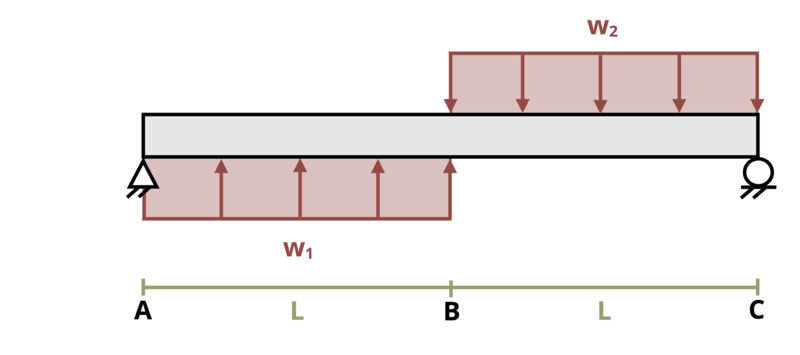
\includegraphics[keepaspectratio]{images/323.png}}
{[}Problem adapted from © Kurt Gramoll CC BY NC-SA 4.0{]}

\begin{Shaded}
\begin{Highlighting}[]
\NormalTok{\#| standalone: true}
\NormalTok{\#| viewerHeight: 600}
\NormalTok{\#| components: [viewer]}

\NormalTok{from shiny import App, render, ui, reactive}
\NormalTok{import random}
\NormalTok{import asyncio}
\NormalTok{import io}
\NormalTok{import math}
\NormalTok{import string}
\NormalTok{from datetime import datetime}
\NormalTok{from pathlib import Path}

\NormalTok{def generate\_random\_letters(length):}
\NormalTok{    \# Generate a random string of letters of specified length}
\NormalTok{    return \textquotesingle{}\textquotesingle{}.join(random.choice(string.ascii\_lowercase) for \_ in range(length))  }

\NormalTok{problem\_ID="323"}
\NormalTok{w1=reactive.Value("\_\_")}
\NormalTok{w2=reactive.Value("\_\_")}
\NormalTok{L=reactive.Value("\_\_")}
  
\NormalTok{attempts=["Timestamp,Attempt,Answer,Feedback\textbackslash{}n"]}

\NormalTok{app\_ui = ui.page\_fluid(}
\NormalTok{    \#ui.markdown("**Please enter your ID number from your instructor and click to generate your problem**"),}
\NormalTok{    \#ui.input\_text("ID","", placeholder="Enter ID Number Here"),}
\NormalTok{    \#ui.input\_action\_button("generate\_problem", "Generate Problem", class\_="btn{-}primary"),}
\NormalTok{    ui.markdown("**Problem Statement**"),}
\NormalTok{    ui.output\_ui("ui\_problem\_statement"),}
\NormalTok{    ui.input\_text("answer","Your Answer in units of kN{-}m", placeholder="Please enter your answer"),}
\NormalTok{    ui.input\_action\_button("submit", "Check Answer", class\_="btn{-}primary"),}
\NormalTok{    \#ui.download\_button("download", "Download File to Submit", class\_="btn{-}success"),}
\NormalTok{)}

\NormalTok{def server(input, output, session):}
\NormalTok{    \# Initialize a counter for attempts}
\NormalTok{    attempt\_counter = reactive.Value(0)}

\NormalTok{    @output}
\NormalTok{    @render.ui}
\NormalTok{    def ui\_problem\_statement():}
\NormalTok{        randomize\_vars()}
\NormalTok{        return[ui.markdown(f"A beam is loaded as shown, where w\textless{}sub\textgreater{}1\textless{}/sub\textgreater{} = \{w1()\} kN/m and w\textless{}sub\textgreater{}2\textless{}/sub\textgreater{} = \{w2()\} kN/m. If length L = \{L()\} m, plot the shear force and bending moment diagrams and determine the magnitude of the maximum absolute bending moment.")]}
    
\NormalTok{    \#@reactive.Effect}
\NormalTok{    \#@reactive.event(input.generate\_problem)}
\NormalTok{    def randomize\_vars():}
\NormalTok{        random.seed(101)}
\NormalTok{        w1.set(random.randrange(10,100,1)/10)}
\NormalTok{        w2.set(w1()+random.randrange(10,50,1)/10)}
\NormalTok{        L.set(random.randrange(20,100,1)/10)}

\NormalTok{    @reactive.Effect}
\NormalTok{    @reactive.event(input.submit)}
\NormalTok{    def \_():}
\NormalTok{        attempt\_counter.set(attempt\_counter() + 1)  \# Increment the attempt counter on each submission.}
\NormalTok{        Ay = (w1()*L()*1.5*L(){-}w2()*L()*L()/2)/(2*L())}
\NormalTok{        Cy = {-}w1()*L(){-}Ay+w2()*L()}
\NormalTok{        x = (Cy{-}2*L()*w2())/({-}w2())}
\NormalTok{        instr = {-}w2()*x**2/2+2*L()*x*w2(){-}2*L()**2*w2()+2*Cy*L(){-}Cy*x}
\NormalTok{        if math.isclose(float(input.answer()), instr, rel\_tol=0.01):}
\NormalTok{            check = "*Correct*"}
\NormalTok{            correct\_indicator = "JL"}
\NormalTok{        else:}
\NormalTok{            check = "*Not Correct.*"}
\NormalTok{            correct\_indicator = "JG"}

\NormalTok{        \# Generate random parts for the encoded attempt.}
\NormalTok{        random\_start = generate\_random\_letters(4)}
\NormalTok{        random\_middle = generate\_random\_letters(4)}
\NormalTok{        random\_end = generate\_random\_letters(4)}
\NormalTok{        \#encoded\_attempt = f"\{random\_start\}\{problem\_ID\}{-}\{random\_middle\}\{attempt\_counter()\}\{correct\_indicator\}{-}\{random\_end\}\{input.ID()\}"}

\NormalTok{        \# Store the most recent encoded attempt in a reactive value so it persists across submissions}
\NormalTok{        \#session.encoded\_attempt = reactive.Value(encoded\_attempt)}

\NormalTok{        \# Append the attempt data to the attempts list without the encoded attempt}
\NormalTok{        attempts.append(f"\{datetime.now()\}, \{attempt\_counter()\}, \{input.answer()\}, \{check\}\textbackslash{}n")}

\NormalTok{        \# Show feedback to the user.}
\NormalTok{        feedback = ui.markdown(f"Your answer of \{input.answer()\} is \{check\}.")}
\NormalTok{        m = ui.modal(}
\NormalTok{            feedback,}
\NormalTok{            title="Feedback",}
\NormalTok{            easy\_close=True}
\NormalTok{        )}
\NormalTok{        ui.modal\_show(m)}

\NormalTok{    \#@render.download(filename=lambda: f"Problem\_Log{-}\{problem\_ID\}{-}\{input.ID()\}.csv")}
\NormalTok{    async def download():}
\NormalTok{        \# Start the CSV with the encoded attempt (without label)}
\NormalTok{        final\_encoded = session.encoded\_attempt() if session.encoded\_attempt is not None else "No attempts"}
\NormalTok{        yield f"\{final\_encoded\}\textbackslash{}n\textbackslash{}n"}
        
\NormalTok{        \# Write the header for the remaining CSV data once}
\NormalTok{        yield "Timestamp,Attempt,Answer,Feedback\textbackslash{}n"}
        
\NormalTok{        \# Write the attempts data, ensure that the header from the attempts list is not written again}
\NormalTok{        for attempt in attempts[1:]:  \# Skip the first element which is the header}
\NormalTok{            await asyncio.sleep(0.25)  \# This delay may not be necessary; adjust as needed}
\NormalTok{            yield attempt}

\NormalTok{\# App installation}
\NormalTok{app = App(app\_ui, server)}
\end{Highlighting}
\end{Shaded}

\chapter*{Problem 7.18 - Shear Force \& Bending Moment
Equations}\label{problem-7.18---shear-force-bending-moment-equations}
\addcontentsline{toc}{chapter}{Problem 7.18 - Shear Force \& Bending
Moment Equations}

\markboth{Problem 7.18 - Shear Force \& Bending Moment
Equations}{Problem 7.18 - Shear Force \& Bending Moment Equations}

\pandocbounded{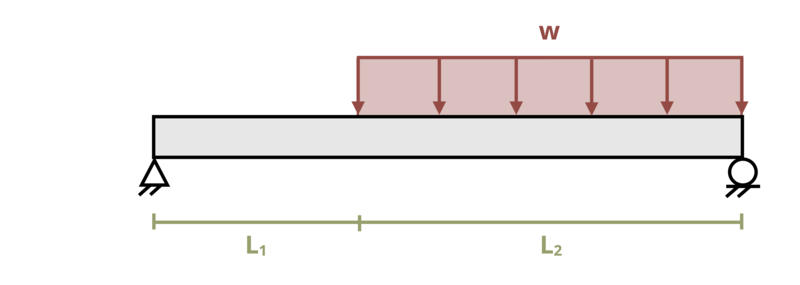
\includegraphics[keepaspectratio]{images/324.png}}
{[}Problem adapted from © Kurt Gramoll CC BY NC-SA 4.0{]}

\begin{Shaded}
\begin{Highlighting}[]
\NormalTok{\#| standalone: true}
\NormalTok{\#| viewerHeight: 600}
\NormalTok{\#| components: [viewer]}

\NormalTok{from shiny import App, render, ui, reactive}
\NormalTok{import random}
\NormalTok{import asyncio}
\NormalTok{import io}
\NormalTok{import math}
\NormalTok{import string}
\NormalTok{from datetime import datetime}
\NormalTok{from pathlib import Path}

\NormalTok{def generate\_random\_letters(length):}
\NormalTok{    \# Generate a random string of letters of specified length}
\NormalTok{    return \textquotesingle{}\textquotesingle{}.join(random.choice(string.ascii\_lowercase) for \_ in range(length))  }

\NormalTok{problem\_ID="324"}
\NormalTok{w=reactive.Value("\_\_")}
\NormalTok{L1=reactive.Value("\_\_")}
\NormalTok{L2=reactive.Value("\_\_")}
  
\NormalTok{attempts=["Timestamp,Attempt,Answer,Feedback\textbackslash{}n"]}

\NormalTok{app\_ui = ui.page\_fluid(}
\NormalTok{    \#ui.markdown("**Please enter your ID number from your instructor and click to generate your problem**"),}
\NormalTok{    \#ui.input\_text("ID","", placeholder="Enter ID Number Here"),}
\NormalTok{    \#ui.input\_action\_button("generate\_problem", "Generate Problem", class\_="btn{-}primary"),}
\NormalTok{    ui.markdown("**Problem Statement**"),}
\NormalTok{    ui.output\_ui("ui\_problem\_statement"),}
\NormalTok{    ui.input\_text("answer","Your Answer in units of kN{-}m", placeholder="Please enter your answer"),}
\NormalTok{    ui.input\_action\_button("submit", "Check Answer", class\_="btn{-}primary"),}
\NormalTok{    \#ui.download\_button("download", "Download File to Submit", class\_="btn{-}success"),}
\NormalTok{)}

\NormalTok{def server(input, output, session):}
\NormalTok{    \# Initialize a counter for attempts}
\NormalTok{    attempt\_counter = reactive.Value(0)}

\NormalTok{    @output}
\NormalTok{    @render.ui}
\NormalTok{    def ui\_problem\_statement():}
\NormalTok{        randomize\_vars()}
\NormalTok{        return[ui.markdown(f"A beam is loaded as shown, where w = \{w()\} kN/m. If lengths L\textless{}sub\textgreater{}1\textless{}/sub\textgreater{} = \{L1()\} m and L\textless{}sub\textgreater{}2\textless{}/sub\textgreater{} = \{L2()\} m, plot the shear force and bending moment diagrams and determine the magnitude of the maximum absolute bending moment.")]}
    
\NormalTok{    \#@reactive.Effect}
\NormalTok{    \#@reactive.event(input.generate\_problem)}
\NormalTok{    def randomize\_vars():}
\NormalTok{        random.seed(101)}
\NormalTok{        w.set(random.randrange(10,300,1)/10)}
\NormalTok{        L1.set(random.randrange(20,80,1)/10)}
\NormalTok{        L2.set(L1()*2)}

\NormalTok{    @reactive.Effect}
\NormalTok{    @reactive.event(input.submit)}
\NormalTok{    def \_():}
\NormalTok{        attempt\_counter.set(attempt\_counter() + 1)  \# Increment the attempt counter on each submission.}
\NormalTok{        Ay = w()*L2()*L2()/2/(L1()+L2())}
\NormalTok{        x = (Ay+w()*L2()/2)/w()}
\NormalTok{        instr = {-}w()*x**2/2+w()/2*x*L2()+Ay*x{-}w()*L2()**2/8}
\NormalTok{        if math.isclose(float(input.answer()), instr, rel\_tol=0.01):}
\NormalTok{            check = "*Correct*"}
\NormalTok{            correct\_indicator = "JL"}
\NormalTok{        else:}
\NormalTok{            check = "*Not Correct.*"}
\NormalTok{            correct\_indicator = "JG"}

\NormalTok{        \# Generate random parts for the encoded attempt.}
\NormalTok{        random\_start = generate\_random\_letters(4)}
\NormalTok{        random\_middle = generate\_random\_letters(4)}
\NormalTok{        random\_end = generate\_random\_letters(4)}
\NormalTok{        \#encoded\_attempt = f"\{random\_start\}\{problem\_ID\}{-}\{random\_middle\}\{attempt\_counter()\}\{correct\_indicator\}{-}\{random\_end\}\{input.ID()\}"}

\NormalTok{        \# Store the most recent encoded attempt in a reactive value so it persists across submissions}
\NormalTok{        \#session.encoded\_attempt = reactive.Value(encoded\_attempt)}

\NormalTok{        \# Append the attempt data to the attempts list without the encoded attempt}
\NormalTok{        attempts.append(f"\{datetime.now()\}, \{attempt\_counter()\}, \{input.answer()\}, \{check\}\textbackslash{}n")}

\NormalTok{        \# Show feedback to the user.}
\NormalTok{        feedback = ui.markdown(f"Your answer of \{input.answer()\} is \{check\}.")}
\NormalTok{        m = ui.modal(}
\NormalTok{            feedback,}
\NormalTok{            title="Feedback",}
\NormalTok{            easy\_close=True}
\NormalTok{        )}
\NormalTok{        ui.modal\_show(m)}

\NormalTok{    \#@render.download(filename=lambda: f"Problem\_Log{-}\{problem\_ID\}{-}\{input.ID()\}.csv")}
\NormalTok{    async def download():}
\NormalTok{        \# Start the CSV with the encoded attempt (without label)}
\NormalTok{        final\_encoded = session.encoded\_attempt() if session.encoded\_attempt is not None else "No attempts"}
\NormalTok{        yield f"\{final\_encoded\}\textbackslash{}n\textbackslash{}n"}
        
\NormalTok{        \# Write the header for the remaining CSV data once}
\NormalTok{        yield "Timestamp,Attempt,Answer,Feedback\textbackslash{}n"}
        
\NormalTok{        \# Write the attempts data, ensure that the header from the attempts list is not written again}
\NormalTok{        for attempt in attempts[1:]:  \# Skip the first element which is the header}
\NormalTok{            await asyncio.sleep(0.25)  \# This delay may not be necessary; adjust as needed}
\NormalTok{            yield attempt}

\NormalTok{\# App installation}
\NormalTok{app = App(app\_ui, server)}
\end{Highlighting}
\end{Shaded}

\chapter*{Problem 7.19 - Shear Force \& Bending Moment
Equations}\label{problem-7.19---shear-force-bending-moment-equations}
\addcontentsline{toc}{chapter}{Problem 7.19 - Shear Force \& Bending
Moment Equations}

\markboth{Problem 7.19 - Shear Force \& Bending Moment
Equations}{Problem 7.19 - Shear Force \& Bending Moment Equations}

\pandocbounded{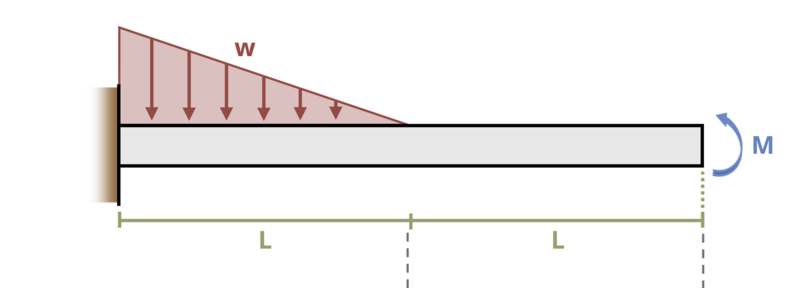
\includegraphics[keepaspectratio]{images/325.png}}
{[}Problem adapted from © Kurt Gramoll CC BY NC-SA 4.0{]}

\begin{Shaded}
\begin{Highlighting}[]
\NormalTok{\#| standalone: true}
\NormalTok{\#| viewerHeight: 600}
\NormalTok{\#| components: [viewer]}

\NormalTok{from shiny import App, render, ui, reactive}
\NormalTok{import random}
\NormalTok{import asyncio}
\NormalTok{import io}
\NormalTok{import math}
\NormalTok{import string}
\NormalTok{from datetime import datetime}
\NormalTok{from pathlib import Path}

\NormalTok{def generate\_random\_letters(length):}
\NormalTok{    \# Generate a random string of letters of specified length}
\NormalTok{    return "".join(random.choice(string.ascii\_lowercase) for \_ in range(length))}

\NormalTok{problem\_ID = "325"}
\NormalTok{w = reactive.Value("\_\_")}
\NormalTok{M = reactive.Value("\_\_")}
\NormalTok{L = reactive.Value("\_\_")}

\NormalTok{attempts = ["Timestamp,Attempt,Answer1,Answer2,Feedback\textbackslash{}n"]}

\NormalTok{app\_ui = ui.page\_fluid(}
\NormalTok{    \#ui.markdown("**Please enter your ID number from your instructor and click to generate your problem**"),}
\NormalTok{    \#ui.input\_text("ID", "", placeholder="Enter ID Number Here"),}
\NormalTok{    \#ui.input\_action\_button("generate\_problem", "Generate Problem", class\_="btn{-}primary"),}
\NormalTok{    ui.markdown("**Problem Statement**"),}
\NormalTok{    ui.output\_ui("ui\_problem\_statement"),}
\NormalTok{    ui.input\_text("answer1", "Your Answer 1 in units of kN", placeholder="Please enter your answer 1"),}
\NormalTok{    ui.input\_text("answer2", "Your Answer 2 in units of kN{-}m", placeholder="Please enter your answer 2"),}
\NormalTok{    ui.input\_action\_button("submit", "Check Answers", class\_="btn{-}primary"),}
\NormalTok{    \#ui.download\_button("download", "Download File to Submit", class\_="btn{-}success"),}
\NormalTok{)}

\NormalTok{def server(input, output, session):}
\NormalTok{    \# Initialize a counter for attempts}
\NormalTok{    attempt\_counter = reactive.Value(0)}

\NormalTok{    @output}
\NormalTok{    @render.ui}
\NormalTok{    def ui\_problem\_statement():}
\NormalTok{        randomize\_vars()}
\NormalTok{        return [ui.markdown(f"Plot the shear force and bending moment diagrams for the loading shown. Assume w = \{w()\} kN/m, M = \{M()\} kN{-}m, and L = \{L()\} m. What is the maximum absolute shear force and maximum absolute bending moment?.")]}

\NormalTok{    \#@reactive.Effect}
\NormalTok{    \#@reactive.event(input.generate\_problem)}
\NormalTok{    def randomize\_vars():}
\NormalTok{        random.seed(101)}
\NormalTok{        w.set(random.randrange(5,30,1))}
\NormalTok{        M.set(random.randrange(5,30,1))}
\NormalTok{        L.set(random.randrange(20,50,1)/10)}
        
\NormalTok{    @reactive.Effect}
\NormalTok{    @reactive.event(input.submit)}
\NormalTok{    def \_():}
\NormalTok{        attempt\_counter.set(}
\NormalTok{            attempt\_counter() + 1}
\NormalTok{        )  \# Increment the attempt counter on each submission.}

\NormalTok{        \# Calculate the instructor\textquotesingle{}s answer and determine if the user\textquotesingle{}s answer is correct.}
\NormalTok{        instr1 = w()*L()/2}
\NormalTok{        instr2 = M()}
              
\NormalTok{        correct1 = math.isclose(float(input.answer1()), instr1, rel\_tol=0.01)}
\NormalTok{        correct2 = math.isclose(float(input.answer2()), instr2, rel\_tol=0.01)}
        
\NormalTok{        if correct1 and correct2:}
\NormalTok{            check = f"\{\textquotesingle{}both correct.\textquotesingle{}\}"}
\NormalTok{        elif correct1:}
\NormalTok{            check = f" \{\textquotesingle{}correct for answer 1 and incorrect for answer 2.\textquotesingle{}\}"}
\NormalTok{        elif correct2:}
\NormalTok{            check = f"\{\textquotesingle{}incorrect for answer 1 and correct for answer 2.\textquotesingle{}\}"}
\NormalTok{        else:}
\NormalTok{            check = f"\{\textquotesingle{}both incorrect.\textquotesingle{}\}"}
        
\NormalTok{        correct\_indicator = "JL" if correct1 and correct2 else "JG"}

\NormalTok{        random\_start = generate\_random\_letters(4)}
\NormalTok{        random\_middle = generate\_random\_letters(4)}
\NormalTok{        random\_end = generate\_random\_letters(4)}
\NormalTok{        \#encoded\_attempt = f"\{random\_start\}\{problem\_ID\}{-}\{random\_middle\}\{attempt\_counter()\}\{correct\_indicator\}{-}\{random\_end\}\{input.ID()\}"}

\NormalTok{        \#session.encoded\_attempt = reactive.Value(encoded\_attempt)}
\NormalTok{        attempts.append(f"\{datetime.now()\}, \{attempt\_counter()\}, \{input.answer1()\}, \{input.answer2()\}, \{check\}\textbackslash{}n")}

\NormalTok{        feedback = ui.markdown(f"Your answers of \{input.answer1()\} and \{input.answer2()\} are \{check\}.")}
\NormalTok{        m = ui.modal(feedback, title="Feedback", easy\_close=True)}
\NormalTok{        ui.modal\_show(m)}

\NormalTok{    \#@render.download(filename=lambda: f"Problem\_Log{-}\{problem\_ID\}{-}\{input.ID()\}.csv")}
\NormalTok{    async def download():}
\NormalTok{        final\_encoded = session.encoded\_attempt() if session.encoded\_attempt is not None else "No attempts"}
\NormalTok{        yield f"\{final\_encoded\}\textbackslash{}n\textbackslash{}n"}
\NormalTok{        yield "Timestamp,Attempt,Answer1,Answer2,Feedback\textbackslash{}n"}
\NormalTok{        for attempt in attempts[1:]:}
\NormalTok{            await asyncio.sleep(0.25)}
\NormalTok{            yield attempt}

\NormalTok{app = App(app\_ui, server)}
\end{Highlighting}
\end{Shaded}

\chapter*{Problem 7.20 - Shear Force \& Bending Moment
Equations}\label{problem-7.20---shear-force-bending-moment-equations}
\addcontentsline{toc}{chapter}{Problem 7.20 - Shear Force \& Bending
Moment Equations}

\markboth{Problem 7.20 - Shear Force \& Bending Moment
Equations}{Problem 7.20 - Shear Force \& Bending Moment Equations}

\pandocbounded{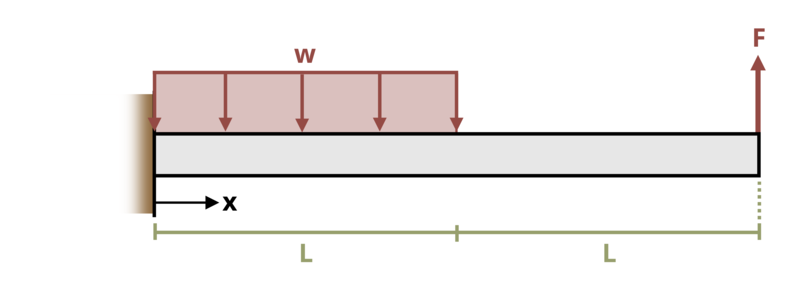
\includegraphics[keepaspectratio]{images/327.png}}
{[}Problem adapted from © Kurt Gramoll CC BY NC-SA 4.0{]}

\begin{Shaded}
\begin{Highlighting}[]
\NormalTok{\#| standalone: true}
\NormalTok{\#| viewerHeight: 600}
\NormalTok{\#| components: [viewer]}

\NormalTok{from shiny import App, render, ui, reactive}
\NormalTok{import random}
\NormalTok{import asyncio}
\NormalTok{import io}
\NormalTok{import math}
\NormalTok{import string}
\NormalTok{from datetime import datetime}
\NormalTok{from pathlib import Path}

\NormalTok{def generate\_random\_letters(length):}
\NormalTok{    \# Generate a random string of letters of specified length}
\NormalTok{    return "".join(random.choice(string.ascii\_lowercase) for \_ in range(length))}

\NormalTok{problem\_ID = "327"}
\NormalTok{w = reactive.Value("\_\_")}
\NormalTok{F = reactive.Value("\_\_")}
\NormalTok{L = reactive.Value("\_\_")}

\NormalTok{attempts = ["Timestamp,Attempt,Answer1,Answer2,Feedback\textbackslash{}n"]}

\NormalTok{app\_ui = ui.page\_fluid(}
\NormalTok{    \#ui.markdown("**Please enter your ID number from your instructor and click to generate your problem**"),}
\NormalTok{    \#ui.input\_text("ID", "", placeholder="Enter ID Number Here"),}
\NormalTok{    \#ui.input\_action\_button("generate\_problem", "Generate Problem", class\_="btn{-}primary"),}
\NormalTok{    ui.markdown("**Problem Statement**"),}
\NormalTok{    ui.output\_ui("ui\_problem\_statement"),}
\NormalTok{    ui.input\_text("answer1", "Your Answer 1 in units of lb", placeholder="Please enter your answer 1"),}
\NormalTok{    ui.input\_text("answer2", "Your Answer 2 in units of lb{-}ft", placeholder="Please enter your answer 2"),}
\NormalTok{    ui.input\_action\_button("submit", "Check Answers", class\_="btn{-}primary"),}
\NormalTok{    \#ui.download\_button("download", "Download File to Submit", class\_="btn{-}success"),}
\NormalTok{)}

\NormalTok{def server(input, output, session):}
\NormalTok{    \# Initialize a counter for attempts}
\NormalTok{    attempt\_counter = reactive.Value(0)}

\NormalTok{    @output}
\NormalTok{    @render.ui}
\NormalTok{    def ui\_problem\_statement():}
\NormalTok{        randomize\_vars()}
\NormalTok{        return [ui.markdown(f"Plot the shear force and bending moment diagrams for the loading shown. Assume w = \{w()\} lb/ft, F = \{F()\} lb, and L = \{L()\} ft. What is the maximum absolute shear force and maximum absolute bending moment?")]}

\NormalTok{    \#@reactive.Effect}
\NormalTok{    \#@reactive.event(input.generate\_problem)}
\NormalTok{    def randomize\_vars():}
\NormalTok{        random.seed(101)}
\NormalTok{        w.set(random.randrange(30,100,1))}
\NormalTok{        F.set(random.randrange(100,300,10))}
\NormalTok{        L.set(random.randrange(20,50,1)/10)}
        
\NormalTok{    @reactive.Effect}
\NormalTok{    @reactive.event(input.submit)}
\NormalTok{    def \_():}
\NormalTok{        attempt\_counter.set(}
\NormalTok{            attempt\_counter() + 1}
\NormalTok{        )  \# Increment the attempt counter on each submission.}

\NormalTok{        \# Calculate the instructor\textquotesingle{}s answer and determine if the user\textquotesingle{}s answer is correct.}
\NormalTok{        instr1 = F()}
\NormalTok{        instr2 = w()*L()*L()/2{-}F()*2*L()}
              
\NormalTok{        correct1 = math.isclose(float(input.answer1()), instr1, rel\_tol=0.01)}
\NormalTok{        correct2 = math.isclose(float(input.answer2()), instr2, rel\_tol=0.01)}
        
\NormalTok{        if correct1 and correct2:}
\NormalTok{            check = f"\{\textquotesingle{}both correct.\textquotesingle{}\}"}
\NormalTok{        elif correct1:}
\NormalTok{            check = f" \{\textquotesingle{}correct for answer 1 and incorrect for answer 2.\textquotesingle{}\}"}
\NormalTok{        elif correct2:}
\NormalTok{            check = f"\{\textquotesingle{}incorrect for answer 1 and correct for answer 2.\textquotesingle{}\}"}
\NormalTok{        else:}
\NormalTok{            check = f"\{\textquotesingle{}both incorrect.\textquotesingle{}\}"}
        
\NormalTok{        correct\_indicator = "JL" if correct1 and correct2 else "JG"}

\NormalTok{        random\_start = generate\_random\_letters(4)}
\NormalTok{        random\_middle = generate\_random\_letters(4)}
\NormalTok{        random\_end = generate\_random\_letters(4)}
\NormalTok{        \#encoded\_attempt = f"\{random\_start\}\{problem\_ID\}{-}\{random\_middle\}\{attempt\_counter()\}\{correct\_indicator\}{-}\{random\_end\}\{input.ID()\}"}

\NormalTok{        \#session.encoded\_attempt = reactive.Value(encoded\_attempt)}
\NormalTok{        attempts.append(f"\{datetime.now()\}, \{attempt\_counter()\}, \{input.answer1()\}, \{input.answer2()\}, \{check\}\textbackslash{}n")}

\NormalTok{        feedback = ui.markdown(f"Your answers of \{input.answer1()\} and \{input.answer2()\} are \{check\}.")}
\NormalTok{        m = ui.modal(feedback, title="Feedback", easy\_close=True)}
\NormalTok{        ui.modal\_show(m)}

\NormalTok{    \#@render.download(filename=lambda: f"Problem\_Log{-}\{problem\_ID\}{-}\{input.ID()\}.csv")}
\NormalTok{    async def download():}
\NormalTok{        final\_encoded = session.encoded\_attempt() if session.encoded\_attempt is not None else "No attempts"}
\NormalTok{        yield f"\{final\_encoded\}\textbackslash{}n\textbackslash{}n"}
\NormalTok{        yield "Timestamp,Attempt,Answer1,Answer2,Feedback\textbackslash{}n"}
\NormalTok{        for attempt in attempts[1:]:}
\NormalTok{            await asyncio.sleep(0.25)}
\NormalTok{            yield attempt}

\NormalTok{app = App(app\_ui, server)}
\end{Highlighting}
\end{Shaded}

\chapter*{Problem 7.21 - Shear Force \& Bending Moment
Equations}\label{problem-7.21---shear-force-bending-moment-equations}
\addcontentsline{toc}{chapter}{Problem 7.21 - Shear Force \& Bending
Moment Equations}

\markboth{Problem 7.21 - Shear Force \& Bending Moment
Equations}{Problem 7.21 - Shear Force \& Bending Moment Equations}

\pandocbounded{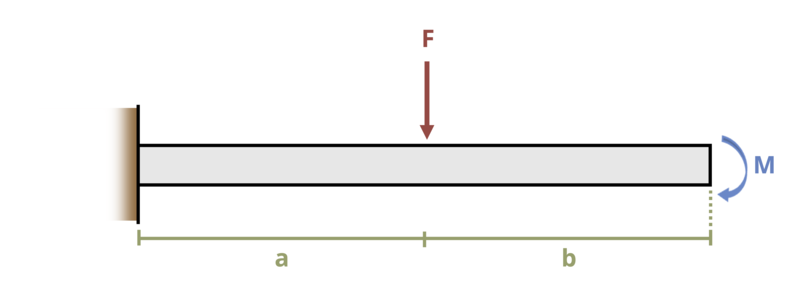
\includegraphics[keepaspectratio]{images/329.png}}
{[}Problem adapted from © Kurt Gramoll CC BY NC-SA 4.0{]}

\begin{Shaded}
\begin{Highlighting}[]
\NormalTok{\#| standalone: true}
\NormalTok{\#| viewerHeight: 600}
\NormalTok{\#| components: [viewer]}

\NormalTok{from shiny import App, render, ui, reactive}
\NormalTok{import random}
\NormalTok{import asyncio}
\NormalTok{import io}
\NormalTok{import math}
\NormalTok{import string}
\NormalTok{from datetime import datetime}
\NormalTok{from pathlib import Path}

\NormalTok{def generate\_random\_letters(length):}
\NormalTok{    \# Generate a random string of letters of specified length}
\NormalTok{    return "".join(random.choice(string.ascii\_lowercase) for \_ in range(length))}

\NormalTok{problem\_ID = "329"}
\NormalTok{F = reactive.Value("\_\_")}
\NormalTok{M = reactive.Value("\_\_")}
\NormalTok{b = reactive.Value("\_\_")}
\NormalTok{a = reactive.Value("\_\_")}
\NormalTok{attempts = ["Timestamp,Attempt,Answer1,Answer2,Feedback\textbackslash{}n"]}

\NormalTok{app\_ui = ui.page\_fluid(}
\NormalTok{    \#ui.markdown("**Please enter your ID number from your instructor and click to generate your problem**"),}
\NormalTok{    \#ui.input\_text("ID", "", placeholder="Enter ID Number Here"),}
\NormalTok{    \#ui.input\_action\_button("generate\_problem", "Generate Problem", class\_="btn{-}primary"),}
\NormalTok{    ui.markdown("**Problem Statement**"),}
\NormalTok{    ui.output\_ui("ui\_problem\_statement"),}
\NormalTok{    ui.input\_text("answer1", "Your Answer 1 in units of lb", placeholder="Please enter your answer 1"),}
\NormalTok{    ui.input\_text("answer2", "Your Answer 2 in units of lb{-}ft", placeholder="Please enter your answer 2"),}
\NormalTok{    ui.input\_action\_button("submit", "Check Answers", class\_="btn{-}primary"),}
\NormalTok{    \#ui.download\_button("download", "Download File to Submit", class\_="btn{-}success"),}
\NormalTok{)}

\NormalTok{def server(input, output, session):}
\NormalTok{    \# Initialize a counter for attempts}
\NormalTok{    attempt\_counter = reactive.Value(0)}

\NormalTok{    @output}
\NormalTok{    @render.ui}
\NormalTok{    def ui\_problem\_statement():}
\NormalTok{        randomize\_vars()}
\NormalTok{        return [}
\NormalTok{            ui.markdown(}
\NormalTok{                f"Plot the shear force and bending moment diagrams for the loading shown. Assume loads F = \{F()\} lb and M = \{M()\} lb{-}ft, and lengths a = \{a()\} ft and b = \{b()\} ft. What is the maximum absolute shear force and maximum absolute bending moment?."}
\NormalTok{            )}
\NormalTok{        ]}

\NormalTok{    \#@reactive.Effect}
\NormalTok{    \#@reactive.event(input.generate\_problem)}
\NormalTok{    def randomize\_vars():}
\NormalTok{        random.seed(101)}
\NormalTok{        F.set(random.randrange(50,200,5))}
\NormalTok{        M.set(random.randrange(250,500,10))}
\NormalTok{        b.set(random.randrange(50,100,1)/10)}
\NormalTok{        a.set(b()+round(random.randrange(10,20,1)/10))}
        
\NormalTok{    @reactive.Effect}
\NormalTok{    @reactive.event(input.submit)}
\NormalTok{    def \_():}
\NormalTok{        attempt\_counter.set(}
\NormalTok{            attempt\_counter() + 1}
\NormalTok{        )  \# Increment the attempt counter on each submission.}

\NormalTok{        \# Calculate the instructor\textquotesingle{}s answer and determine if the user\textquotesingle{}s answer is correct.}
\NormalTok{        instr1 = F()}
\NormalTok{        instr2 = F()*a()+M()}

\NormalTok{        correct1 = math.isclose(float(input.answer1()), instr1, rel\_tol=0.01)}
\NormalTok{        correct2 = math.isclose(float(input.answer2()), instr2, rel\_tol=0.01)}
        
\NormalTok{        if correct1 and correct2:}
\NormalTok{            check = f"\{\textquotesingle{}both correct.\textquotesingle{}\}"}
\NormalTok{        elif correct1:}
\NormalTok{            check = f" \{\textquotesingle{}correct for answer 1 and incorrect for answer 2.\textquotesingle{}\}"}
\NormalTok{        elif correct2:}
\NormalTok{            check = f"\{\textquotesingle{}incorrect for answer 1 and correct for answer 2.\textquotesingle{}\}"}
\NormalTok{        else:}
\NormalTok{            check = f"\{\textquotesingle{}both incorrect.\textquotesingle{}\}"}
        
\NormalTok{        correct\_indicator = "JL" if correct1 and correct2 else "JG"}

\NormalTok{        random\_start = generate\_random\_letters(4)}
\NormalTok{        random\_middle = generate\_random\_letters(4)}
\NormalTok{        random\_end = generate\_random\_letters(4)}
\NormalTok{        \#encoded\_attempt = f"\{random\_start\}\{problem\_ID\}{-}\{random\_middle\}\{attempt\_counter()\}\{correct\_indicator\}{-}\{random\_end\}\{input.ID()\}"}

\NormalTok{        \#session.encoded\_attempt = reactive.Value(encoded\_attempt)}
\NormalTok{        attempts.append(f"\{datetime.now()\}, \{attempt\_counter()\}, \{input.answer1()\}, \{input.answer2()\}, \{check\}\textbackslash{}n")}

\NormalTok{        feedback = ui.markdown(f"Your answers of \{input.answer1()\} and \{input.answer2()\} are \{check\}.")}
\NormalTok{        m = ui.modal(feedback, title="Feedback", easy\_close=True)}
\NormalTok{        ui.modal\_show(m)}

\NormalTok{    \#@render.download(filename=lambda: f"Problem\_Log{-}\{problem\_ID\}{-}\{input.ID()\}.csv")}
\NormalTok{    async def download():}
\NormalTok{        final\_encoded = session.encoded\_attempt() if session.encoded\_attempt is not None else "No attempts"}
\NormalTok{        yield f"\{final\_encoded\}\textbackslash{}n\textbackslash{}n"}
\NormalTok{        yield "Timestamp,Attempt,Answer1,Answer2,Feedback\textbackslash{}n"}
\NormalTok{        for attempt in attempts[1:]:}
\NormalTok{            await asyncio.sleep(0.25)}
\NormalTok{            yield attempt}

\NormalTok{app = App(app\_ui, server)}
\end{Highlighting}
\end{Shaded}

\chapter*{Problem 7.22 - Determining Equations by
Integration}\label{problem-7.22---determining-equations-by-integration}
\addcontentsline{toc}{chapter}{Problem 7.22 - Determining Equations by
Integration}

\markboth{Problem 7.22 - Determining Equations by Integration}{Problem
7.22 - Determining Equations by Integration}

\pandocbounded{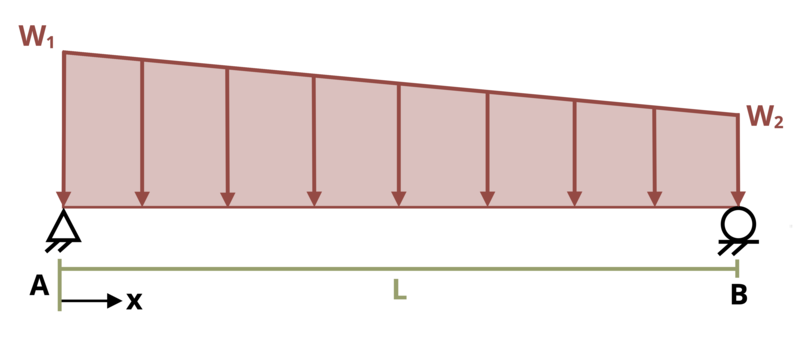
\includegraphics[keepaspectratio]{images/672.png}}
{[}Problem adapted from © Chris Galitz CC BY NC-SA 4.0{]}

\begin{Shaded}
\begin{Highlighting}[]
\NormalTok{\#| standalone: true}
\NormalTok{\#| viewerHeight: 600}
\NormalTok{\#| components: [viewer]}

\NormalTok{from shiny import App, render, ui, reactive}
\NormalTok{import random}
\NormalTok{import asyncio}
\NormalTok{import io}
\NormalTok{import math}
\NormalTok{import string}
\NormalTok{from datetime import datetime}
\NormalTok{from pathlib import Path}

\NormalTok{def generate\_random\_letters(length):}
\NormalTok{    \# Generate a random string of letters of specified length}
\NormalTok{    return "".join(random.choice(string.ascii\_lowercase) for \_ in range(length))}

\NormalTok{problem\_ID = "672"}
\NormalTok{w1 = reactive.Value("\_\_")}
\NormalTok{w2 = reactive.Value("\_\_")}
\NormalTok{L = reactive.Value("\_\_")}
\NormalTok{attempts = ["Timestamp,Attempt,Answer1,Answer2,Feedback\textbackslash{}n"]}

\NormalTok{app\_ui = ui.page\_fluid(}
\NormalTok{    \#ui.markdown("**Please enter your ID number from your instructor and click to generate your problem**"),}
\NormalTok{    \#ui.input\_text("ID", "", placeholder="Enter ID Number Here"),}
\NormalTok{    \#ui.input\_action\_button("generate\_problem", "Generate Problem", class\_="btn{-}primary"),}
\NormalTok{    ui.markdown("**Problem Statement**"),}
\NormalTok{    ui.output\_ui("ui\_problem\_statement"),}
\NormalTok{    ui.input\_text("answer1", "Your Answer 1 in units of kN", placeholder="Please enter your answer 1"),}
\NormalTok{    ui.input\_text("answer2", "Your Answer 2 in units of kN{-}m", placeholder="Please enter your answer 2"),}
\NormalTok{    ui.input\_action\_button("submit", "Check Answers", class\_="btn{-}primary"),}
\NormalTok{    \#ui.download\_button("download", "Download File to Submit", class\_="btn{-}success"),}
\NormalTok{)}

\NormalTok{def server(input, output, session):}
\NormalTok{    \# Initialize a counter for attempts}
\NormalTok{    attempt\_counter = reactive.Value(0)}

\NormalTok{    @output}
\NormalTok{    @render.ui}
\NormalTok{    def ui\_problem\_statement():}
\NormalTok{        randomize\_vars()}
\NormalTok{        return [}
\NormalTok{            ui.markdown(}
\NormalTok{                f"A simply supported beam supports a trapezoidal load function with ω\textless{}sub\textgreater{}1\textless{}/sub\textgreater{} = \{w1()\} kN/m and ω\textless{}sub\textgreater{}2\textless{}/sub\textgreater{} = \{w2()\} kN/m. For a bem length L = \{L()\} m, derive the equations for beam shear, V(x), and bending moment, M(x). Determine the maximum magnitude for each."}
\NormalTok{            )}
\NormalTok{        ]}

\NormalTok{    \#@reactive.Effect}
\NormalTok{    \#@reactive.event(input.generate\_problem)}
\NormalTok{    def randomize\_vars():}
\NormalTok{        random.seed(101)}
\NormalTok{        w1.set(random.randrange(30,60,1))}
\NormalTok{        w2.set(w1(){-}random.randrange(10,20,1))}
\NormalTok{        L.set(random.randrange(5,15,1))}
        
\NormalTok{    @reactive.Effect}
\NormalTok{    @reactive.event(input.submit)}
\NormalTok{    def \_():}
\NormalTok{        attempt\_counter.set(}
\NormalTok{            attempt\_counter() + 1}
\NormalTok{        )  \# Increment the attempt counter on each submission.}

\NormalTok{        \# Calculate the instructor\textquotesingle{}s answer and determine if the user\textquotesingle{}s answer is correct.}
\NormalTok{        C1=w1()*L()/3+w2()*L()/6  }
\NormalTok{        instr1 = C1}
\NormalTok{        x=(w1(){-}math.sqrt(w1()**2{-}4*(w1()/(2*L()){-}w2()/(2*L()))*C1))/(2*(w1()/(2*L()){-}w2()/(2*L())))            }
\NormalTok{        instr2 = {-}w1()*x**2/2+w1()*x**3/(6*L()){-}w2()*x**3/(6*L())+C1*x}

\NormalTok{        correct1 = math.isclose(float(input.answer1()), instr1, rel\_tol=0.01)}
\NormalTok{        correct2 = math.isclose(float(input.answer2()), instr2, rel\_tol=0.01)}
        
\NormalTok{        if correct1 and correct2:}
\NormalTok{            check = f"\{\textquotesingle{}both correct.\textquotesingle{}\}"}
\NormalTok{        elif correct1:}
\NormalTok{            check = f" \{\textquotesingle{}correct for answer 1 and incorrect for answer 2.\textquotesingle{}\}"}
\NormalTok{        elif correct2:}
\NormalTok{            check = f"\{\textquotesingle{}incorrect for answer 1 and correct for answer 2.\textquotesingle{}\}"}
\NormalTok{        else:}
\NormalTok{            check = f"\{\textquotesingle{}both incorrect.\textquotesingle{}\}"}
        
\NormalTok{        correct\_indicator = "JL" if correct1 and correct2 else "JG"}

\NormalTok{        random\_start = generate\_random\_letters(4)}
\NormalTok{        random\_middle = generate\_random\_letters(4)}
\NormalTok{        random\_end = generate\_random\_letters(4)}
\NormalTok{        \#encoded\_attempt = f"\{random\_start\}\{problem\_ID\}{-}\{random\_middle\}\{attempt\_counter()\}\{correct\_indicator\}{-}\{random\_end\}\{input.ID()\}"}

\NormalTok{        \#session.encoded\_attempt = reactive.Value(encoded\_attempt)}
\NormalTok{        attempts.append(f"\{datetime.now()\}, \{attempt\_counter()\}, \{input.answer1()\}, \{input.answer2()\}, \{check\}\textbackslash{}n")}

\NormalTok{        feedback = ui.markdown(f"Your answers of \{input.answer1()\} and \{input.answer2()\} are \{check\}.")}
\NormalTok{        m = ui.modal(feedback, title="Feedback", easy\_close=True)}
\NormalTok{        ui.modal\_show(m)}

\NormalTok{    \#@render.download(filename=lambda: f"Problem\_Log{-}\{problem\_ID\}{-}\{input.ID()\}.csv")}
\NormalTok{    async def download():}
\NormalTok{        final\_encoded = session.encoded\_attempt() if session.encoded\_attempt is not None else "No attempts"}
\NormalTok{        yield f"\{final\_encoded\}\textbackslash{}n\textbackslash{}n"}
\NormalTok{        yield "Timestamp,Attempt,Answer1,Answer2,Feedback\textbackslash{}n"}
\NormalTok{        for attempt in attempts[1:]:}
\NormalTok{            await asyncio.sleep(0.25)}
\NormalTok{            yield attempt}

\NormalTok{app = App(app\_ui, server)}
\end{Highlighting}
\end{Shaded}

\chapter*{Problem 7.23 - Determining Equations by
Integration}\label{problem-7.23---determining-equations-by-integration}
\addcontentsline{toc}{chapter}{Problem 7.23 - Determining Equations by
Integration}

\markboth{Problem 7.23 - Determining Equations by Integration}{Problem
7.23 - Determining Equations by Integration}

\pandocbounded{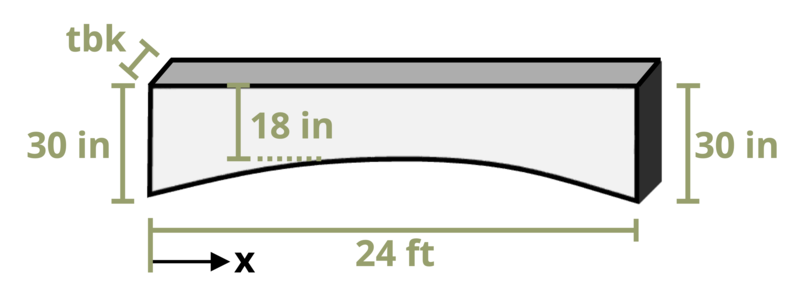
\includegraphics[keepaspectratio]{images/673.png}}
{[}Problem adapted from © Chris Galitz CC BY NC-SA 4.0{]}

\begin{Shaded}
\begin{Highlighting}[]
\NormalTok{\#| standalone: true}
\NormalTok{\#| viewerHeight: 600}
\NormalTok{\#| components: [viewer]}

\NormalTok{from shiny import App, render, ui, reactive}
\NormalTok{import random}
\NormalTok{import asyncio}
\NormalTok{import io}
\NormalTok{import math}
\NormalTok{import string}
\NormalTok{from datetime import datetime}
\NormalTok{from pathlib import Path}

\NormalTok{def generate\_random\_letters(length):}
\NormalTok{    \# Generate a random string of letters of specified length}
\NormalTok{    return "".join(random.choice(string.ascii\_lowercase) for \_ in range(length))}

\NormalTok{problem\_ID = "673"}
\NormalTok{t = reactive.Value("\_\_")}
\NormalTok{w = reactive.Value("\_\_")}
\NormalTok{attempts = ["Timestamp,Attempt,Answer1,Answer2,Feedback\textbackslash{}n"]}

\NormalTok{app\_ui = ui.page\_fluid(}
\NormalTok{    \#ui.markdown("**Please enter your ID number from your instructor and click to generate your problem**"),}
\NormalTok{    \#ui.input\_text("ID", "", placeholder="Enter ID Number Here"),}
\NormalTok{    \#ui.input\_action\_button("generate\_problem", "Generate Problem", class\_="btn{-}primary"),}
\NormalTok{    ui.markdown("**Problem Statement**"),}
\NormalTok{    ui.output\_ui("ui\_problem\_statement"),}
\NormalTok{    ui.input\_text("answer1", "Your Answer 1 in units of lb", placeholder="Please enter your answer 1"),}
\NormalTok{    ui.input\_text("answer2", "Your Answer 2 in units of lb{-}ft", placeholder="Please enter your answer 2"),}
\NormalTok{    ui.input\_action\_button("submit", "Check Answers", class\_="btn{-}primary"),}
\NormalTok{    \#ui.download\_button("download", "Download File to Submit", class\_="btn{-}success"),}
\NormalTok{)}

\NormalTok{def server(input, output, session):}
\NormalTok{    \# Initialize a counter for attempts}
\NormalTok{    attempt\_counter = reactive.Value(0)}

\NormalTok{    @output}
\NormalTok{    @render.ui}
\NormalTok{    def ui\_problem\_statement():}
\NormalTok{        randomize\_vars()}
\NormalTok{        return [}
\NormalTok{            ui.markdown(}
\NormalTok{                f"A parabolic arch is formed by the simply{-}supported precast concrete piece shown. Assuming the concrete has a thickness t = \{t()\} inches and a unit weight w = \{w()\} lb per cubic foot, derive the equations for beam shear, V(x) and bending moment, M(x), in the concrete. Determine the maximum magnitude for each. The height of the arch, in feet, is given by the equation h(x) = 1/144*x\textless{}sup\textgreater{}2\textless{}/sup\textgreater{} {-} 1/6*x + 2.5."}
\NormalTok{            )}
\NormalTok{        ]}

\NormalTok{    \#@reactive.Effect}
\NormalTok{    \#@reactive.event(input.generate\_problem)}
\NormalTok{    def randomize\_vars():}
\NormalTok{        random.seed(101)}
\NormalTok{        t.set(random.randrange(6,18,1))}
\NormalTok{        w.set(random.randrange(125,175,1))}
        
\NormalTok{    @reactive.Effect}
\NormalTok{    @reactive.event(input.submit)}
\NormalTok{    def \_():}
\NormalTok{        attempt\_counter.set(}
\NormalTok{            attempt\_counter() + 1}
\NormalTok{        )  \# Increment the attempt counter on each submission.}

\NormalTok{        \# Calculate the instructor\textquotesingle{}s answer and determine if the user\textquotesingle{}s answer is correct.}
\NormalTok{        L=24}
\NormalTok{        wxa={-}1/144*t()*w()}
\NormalTok{        wxb=1/6*t()*w()}
\NormalTok{        wxc={-}2.5*t()*w()}
\NormalTok{        x=L/2}
\NormalTok{        instr1=1/L*({-}wxa/12*L**4{-}wxb/6*L**3{-}wxc/2*L**2)}
\NormalTok{        instr2=wxa/12*x**4+wxb/6*x**3+wxc/2*x**2+instr1*x}

\NormalTok{        correct1 = math.isclose(float(input.answer1()), instr1, rel\_tol=0.01)}
\NormalTok{        correct2 = math.isclose(float(input.answer2()), instr2, rel\_tol=0.01)}
        
\NormalTok{        if correct1 and correct2:}
\NormalTok{            check = f"\{\textquotesingle{}both correct.\textquotesingle{}\}"}
\NormalTok{        elif correct1:}
\NormalTok{            check = f" \{\textquotesingle{}correct for answer 1 and incorrect for answer 2.\textquotesingle{}\}"}
\NormalTok{        elif correct2:}
\NormalTok{            check = f"\{\textquotesingle{}incorrect for answer 1 and correct for answer 2.\textquotesingle{}\}"}
\NormalTok{        else:}
\NormalTok{            check = f"\{\textquotesingle{}both incorrect.\textquotesingle{}\}"}
        
\NormalTok{        correct\_indicator = "JL" if correct1 and correct2 else "JG"}

\NormalTok{        random\_start = generate\_random\_letters(4)}
\NormalTok{        random\_middle = generate\_random\_letters(4)}
\NormalTok{        random\_end = generate\_random\_letters(4)}
\NormalTok{        \#encoded\_attempt = f"\{random\_start\}\{problem\_ID\}{-}\{random\_middle\}\{attempt\_counter()\}\{correct\_indicator\}{-}\{random\_end\}\{input.ID()\}"}

\NormalTok{        \#session.encoded\_attempt = reactive.Value(encoded\_attempt)}
\NormalTok{        attempts.append(f"\{datetime.now()\}, \{attempt\_counter()\}, \{input.answer1()\}, \{input.answer2()\}, \{check\}\textbackslash{}n")}

\NormalTok{        feedback = ui.markdown(f"Your answers of \{input.answer1()\} and \{input.answer2()\} are \{check\}")}
\NormalTok{        m = ui.modal(feedback, title="Feedback", easy\_close=True)}
\NormalTok{        ui.modal\_show(m)}

\NormalTok{    \#@render.download(filename=lambda: f"Problem\_Log{-}\{problem\_ID\}{-}\{input.ID()\}.csv")}
\NormalTok{    async def download():}
\NormalTok{        final\_encoded = session.encoded\_attempt() if session.encoded\_attempt is not None else "No attempts"}
\NormalTok{        yield f"\{final\_encoded\}\textbackslash{}n\textbackslash{}n"}
\NormalTok{        yield "Timestamp,Attempt,Answer1,Answer2,Feedback\textbackslash{}n"}
\NormalTok{        for attempt in attempts[1:]:}
\NormalTok{            await asyncio.sleep(0.25)}
\NormalTok{            yield attempt}

\NormalTok{app = App(app\_ui, server)}
\end{Highlighting}
\end{Shaded}

\chapter*{Problem 7.24 - Determining Equations by
Integration}\label{problem-7.24---determining-equations-by-integration}
\addcontentsline{toc}{chapter}{Problem 7.24 - Determining Equations by
Integration}

\markboth{Problem 7.24 - Determining Equations by Integration}{Problem
7.24 - Determining Equations by Integration}

\pandocbounded{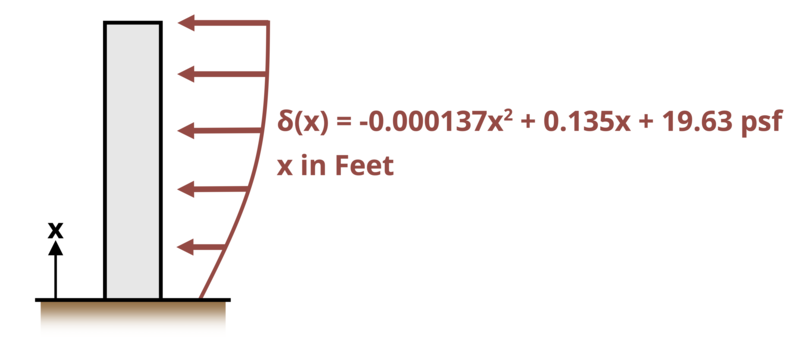
\includegraphics[keepaspectratio]{images/674.png}}
{[}Problem adapted from © Chris Galitz CC BY NC-SA 4.0{]}

\begin{Shaded}
\begin{Highlighting}[]
\NormalTok{\#| standalone: true}
\NormalTok{\#| viewerHeight: 600}
\NormalTok{\#| components: [viewer]}

\NormalTok{from shiny import App, render, ui, reactive}
\NormalTok{import random}
\NormalTok{import asyncio}
\NormalTok{import io}
\NormalTok{import math}
\NormalTok{import string}
\NormalTok{from datetime import datetime}
\NormalTok{from pathlib import Path}

\NormalTok{def generate\_random\_letters(length):}
\NormalTok{    \# Generate a random string of letters of specified length}
\NormalTok{    return "".join(random.choice(string.ascii\_lowercase) for \_ in range(length))}

\NormalTok{problem\_ID = "674"}
\NormalTok{w = reactive.Value("\_\_")}
\NormalTok{h = reactive.Value("\_\_")}
\NormalTok{attempts = ["Timestamp,Attempt,Answer1,Answer2,Feedback\textbackslash{}n"]}

\NormalTok{app\_ui = ui.page\_fluid(}
\NormalTok{    \#ui.markdown("**Please enter your ID number from your instructor and click to generate your problem**"),}
\NormalTok{    \#ui.input\_text("ID", "", placeholder="Enter ID Number Here"),}
\NormalTok{    \#ui.input\_action\_button("generate\_problem", "Generate Problem", class\_="btn{-}primary"),}
\NormalTok{    ui.markdown("**Problem Statement**"),}
\NormalTok{    ui.output\_ui("ui\_problem\_statement"),}
\NormalTok{    ui.input\_text("answer1", "Your Answer 1 in units of lb", placeholder="Please enter your answer 1"),}
\NormalTok{    ui.input\_text("answer2", "Your Answer 2 in units of lb{-}ft", placeholder="Please enter your answer 2"),}
\NormalTok{    ui.input\_action\_button("submit", "Check Answers", class\_="btn{-}primary"),}
\NormalTok{    \#ui.download\_button("download", "Download File to Submit", class\_="btn{-}success"),}
\NormalTok{)}

\NormalTok{def server(input, output, session):}
\NormalTok{    \# Initialize a counter for attempts}
\NormalTok{    attempt\_counter = reactive.Value(0)}

\NormalTok{    @output}
\NormalTok{    @render.ui}
\NormalTok{    def ui\_problem\_statement():}
\NormalTok{        randomize\_vars()}
\NormalTok{        return [}
\NormalTok{            ui.markdown(}
\NormalTok{                f"The preliminary design of tall buldings often starts by considering the building as a vertical cantilever subject to a code{-}defined quadratic wind pressure profile. Determine the shear and moment equations for a building of width w = \{w()\} ft and height h = \{h()\} ft and then determine the magnitude of the shear force and bending moment at the mid{-}height of the building."}
\NormalTok{            )}
\NormalTok{        ]}

\NormalTok{    \#@reactive.Effect}
\NormalTok{    \#@reactive.event(input.generate\_problem)}
\NormalTok{    def randomize\_vars():}
\NormalTok{        random.seed(101)}
\NormalTok{        w.set(random.randrange(100,200,5))}
\NormalTok{        h.set(random.randrange(100,300,10))}
        
\NormalTok{    @reactive.Effect}
\NormalTok{    @reactive.event(input.submit)}
\NormalTok{    def \_():}
\NormalTok{        attempt\_counter.set(}
\NormalTok{            attempt\_counter() + 1}
\NormalTok{        )  \# Increment the attempt counter on each submission.}

\NormalTok{        \# Calculate the instructor\textquotesingle{}s answer and determine if the user\textquotesingle{}s answer is correct.}
\NormalTok{        wxa={-}0.000187*{-}w()}
\NormalTok{        wxb=0.145*{-}w()}
\NormalTok{        wxc=19.63*{-}w()}
\NormalTok{        C1={-}wxa/3*h()**3{-}wxb/2*h()**2{-}wxc*h()}
\NormalTok{        C2={-}wxa/12*h()**4{-}wxb/6*h()**3{-}wxc/2*h()**2{-}C1*h()}
\NormalTok{        x=h()/2}
\NormalTok{        instr1=wxa/3*x**3+wxb/2*x**2+wxc*x+C1}
\NormalTok{        instr2=wxa/12*x**4+wxb/6*x**3+wxc/2*x**2+C1*x+C2}

\NormalTok{        correct1 = math.isclose(float(input.answer1()), instr1, rel\_tol=0.01)}
\NormalTok{        correct2 = math.isclose(float(input.answer2()), instr2, rel\_tol=0.01)}
        
\NormalTok{        if correct1 and correct2:}
\NormalTok{            check = f"\{\textquotesingle{}both correct.\textquotesingle{}\}"}
\NormalTok{        elif correct1:}
\NormalTok{            check = f" \{\textquotesingle{}correct for answer 1 and incorrect for answer 2.\textquotesingle{}\}"}
\NormalTok{        elif correct2:}
\NormalTok{            check = f"\{\textquotesingle{}incorrect for answer 1 and correct for answer 2.\textquotesingle{}\}"}
\NormalTok{        else:}
\NormalTok{            check = f"\{\textquotesingle{}both incorrect.\textquotesingle{}\}"}
        
\NormalTok{        correct\_indicator = "JL" if correct1 and correct2 else "JG"}

\NormalTok{        random\_start = generate\_random\_letters(4)}
\NormalTok{        random\_middle = generate\_random\_letters(4)}
\NormalTok{        random\_end = generate\_random\_letters(4)}
\NormalTok{        \#encoded\_attempt = f"\{random\_start\}\{problem\_ID\}{-}\{random\_middle\}\{attempt\_counter()\}\{correct\_indicator\}{-}\{random\_end\}\{input.ID()\}"}

\NormalTok{        \#session.encoded\_attempt = reactive.Value(encoded\_attempt)}
\NormalTok{        attempts.append(f"\{datetime.now()\}, \{attempt\_counter()\}, \{input.answer1()\}, \{input.answer2()\}, \{check\}\textbackslash{}n")}

\NormalTok{        feedback = ui.markdown(f"Your answers of \{input.answer1()\} and \{input.answer2()\} are \{check\}")}
\NormalTok{        m = ui.modal(feedback, title="Feedback", easy\_close=True)}
\NormalTok{        ui.modal\_show(m)}

\NormalTok{    \#@render.download(filename=lambda: f"Problem\_Log{-}\{problem\_ID\}{-}\{input.ID()\}.csv")}
\NormalTok{    async def download():}
\NormalTok{        final\_encoded = session.encoded\_attempt() if session.encoded\_attempt is not None else "No attempts"}
\NormalTok{        yield f"\{final\_encoded\}\textbackslash{}n\textbackslash{}n"}
\NormalTok{        yield "Timestamp,Attempt,Answer1,Answer2,Feedback\textbackslash{}n"}
\NormalTok{        for attempt in attempts[1:]:}
\NormalTok{            await asyncio.sleep(0.25)}
\NormalTok{            yield attempt}

\NormalTok{app = App(app\_ui, server)}
\end{Highlighting}
\end{Shaded}

\chapter*{Problem 7.25 - Graphical Methods for Shear Force \& Bending
Moment
Diagrams}\label{problem-7.25---graphical-methods-for-shear-force-bending-moment-diagrams}
\addcontentsline{toc}{chapter}{Problem 7.25 - Graphical Methods for
Shear Force \& Bending Moment Diagrams}

\markboth{Problem 7.25 - Graphical Methods for Shear Force \& Bending
Moment Diagrams}{Problem 7.25 - Graphical Methods for Shear Force \&
Bending Moment Diagrams}

\pandocbounded{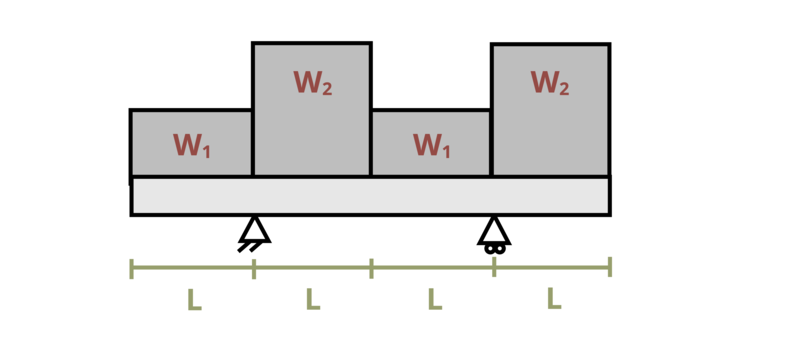
\includegraphics[keepaspectratio]{images/321.png}}
{[}Problem adapted from © Kurt Gramoll CC BY NC-SA 4.0{]}

\begin{Shaded}
\begin{Highlighting}[]
\NormalTok{\#| standalone: true}
\NormalTok{\#| viewerHeight: 600}
\NormalTok{\#| components: [viewer]}

\NormalTok{from shiny import App, render, ui, reactive}
\NormalTok{import random}
\NormalTok{import asyncio}
\NormalTok{import io}
\NormalTok{import math}
\NormalTok{import string}
\NormalTok{from datetime import datetime}
\NormalTok{from pathlib import Path}

\NormalTok{def generate\_random\_letters(length):}
\NormalTok{    \# Generate a random string of letters of specified length}
\NormalTok{    return \textquotesingle{}\textquotesingle{}.join(random.choice(string.ascii\_lowercase) for \_ in range(length))  }

\NormalTok{problem\_ID="321"}
\NormalTok{W1=reactive.Value("\_\_")}
\NormalTok{W2=reactive.Value("\_\_")}
\NormalTok{L=reactive.Value("\_\_")}
  
\NormalTok{attempts=["Timestamp,Attempt,Answer,Feedback\textbackslash{}n"]}

\NormalTok{app\_ui = ui.page\_fluid(}
\NormalTok{    \#ui.markdown("**Please enter your ID number from your instructor and click to generate your problem**"),}
\NormalTok{    \#ui.input\_text("ID","", placeholder="Enter ID Number Here"),}
\NormalTok{    \#ui.input\_action\_button("generate\_problem", "Generate Problem", class\_="btn{-}primary"),}
\NormalTok{    ui.markdown("**Problem Statement**"),}
\NormalTok{    ui.output\_ui("ui\_problem\_statement"),}
\NormalTok{    ui.input\_text("answer","Your Answer in units of lb", placeholder="Please enter your answer"),}
\NormalTok{    ui.input\_action\_button("submit", "Check Answer", class\_="btn{-}primary"),}
\NormalTok{    \#ui.download\_button("download", "Download File to Submit", class\_="btn{-}success"),}
\NormalTok{)}

\NormalTok{def server(input, output, session):}
\NormalTok{    \# Initialize a counter for attempts}
\NormalTok{    attempt\_counter = reactive.Value(0)}

\NormalTok{    @output}
\NormalTok{    @render.ui}
\NormalTok{    def ui\_problem\_statement():}
\NormalTok{        randomize\_vars()}
\NormalTok{        return[ui.markdown(f"A shelf is loaded with four boxes as shown. Assume W\textless{}sub\textgreater{}1\textless{}/sub\textgreater{} = \{W1()\} lb, W\textless{}sub\textgreater{}2\textless{}/sub\textgreater{} = \{W2()\} lb, and L = \{L()\} ft. Determine the maximum internal shear force.")]}
    
\NormalTok{    \#@reactive.Effect}
\NormalTok{    \#@reactive.event(input.generate\_problem)}
\NormalTok{    def randomize\_vars():}
\NormalTok{        random.seed(101)}
\NormalTok{        W1.set(random.randrange(5,75,1))}
\NormalTok{        W2.set(W1()*2)}
\NormalTok{        L.set(random.randrange(10,50,1)/10)}
        
\NormalTok{    @reactive.Effect}
\NormalTok{    @reactive.event(input.submit)}
\NormalTok{    def \_():}
\NormalTok{        attempt\_counter.set(attempt\_counter() + 1)  \# Increment the attempt counter on each submission.}
\NormalTok{        R2 = ({-}W1()*L()/2+W2()*L()/2+W1()*1.5*L()+W2()*2.5*L())/(2*L())}
\NormalTok{        R1 = 2*W1()+2*W2(){-}R2}
\NormalTok{        V1 = {-}W1()}
\NormalTok{        V2 = V1+R1}
\NormalTok{        V3 = V2{-}W2()}
\NormalTok{        V4 = V3{-}W1()}
\NormalTok{        V5 = V4+R2}
\NormalTok{        instr = max(abs(V1), abs(V2), abs(V3), abs(V4), abs(V5))}

\NormalTok{        if math.isclose(float(input.answer()), instr, rel\_tol=0.01):}
\NormalTok{            check = "*Correct*"}
\NormalTok{            correct\_indicator = "JL"}
\NormalTok{        else:}
\NormalTok{            check = "*Not Correct.*"}
\NormalTok{            correct\_indicator = "JG"}

\NormalTok{        \# Generate random parts for the encoded attempt.}
\NormalTok{        random\_start = generate\_random\_letters(4)}
\NormalTok{        random\_middle = generate\_random\_letters(4)}
\NormalTok{        random\_end = generate\_random\_letters(4)}
\NormalTok{        \#encoded\_attempt = f"\{random\_start\}\{problem\_ID\}{-}\{random\_middle\}\{attempt\_counter()\}\{correct\_indicator\}{-}\{random\_end\}\{input.ID()\}"}

\NormalTok{        \# Store the most recent encoded attempt in a reactive value so it persists across submissions}
\NormalTok{        \#session.encoded\_attempt = reactive.Value(encoded\_attempt)}

\NormalTok{        \# Append the attempt data to the attempts list without the encoded attempt}
\NormalTok{        attempts.append(f"\{datetime.now()\}, \{attempt\_counter()\}, \{input.answer()\}, \{check\}\textbackslash{}n")}

\NormalTok{        \# Show feedback to the user.}
\NormalTok{        feedback = ui.markdown(f"Your answer of \{input.answer()\} is \{check\}.")}
\NormalTok{        m = ui.modal(}
\NormalTok{            feedback,}
\NormalTok{            title="Feedback",}
\NormalTok{            easy\_close=True}
\NormalTok{        )}
\NormalTok{        ui.modal\_show(m)}

\NormalTok{    \#@render.download(filename=lambda: f"Problem\_Log{-}\{problem\_ID\}{-}\{input.ID()\}.csv")}
\NormalTok{    async def download():}
\NormalTok{        \# Start the CSV with the encoded attempt (without label)}
\NormalTok{        final\_encoded = session.encoded\_attempt() if session.encoded\_attempt is not None else "No attempts"}
\NormalTok{        yield f"\{final\_encoded\}\textbackslash{}n\textbackslash{}n"}
        
\NormalTok{        \# Write the header for the remaining CSV data once}
\NormalTok{        yield "Timestamp,Attempt,Answer,Feedback\textbackslash{}n"}
        
\NormalTok{        \# Write the attempts data, ensure that the header from the attempts list is not written again}
\NormalTok{        for attempt in attempts[1:]:  \# Skip the first element which is the header}
\NormalTok{            await asyncio.sleep(0.25)  \# This delay may not be necessary; adjust as needed}
\NormalTok{            yield attempt}

\NormalTok{\# App installation}
\NormalTok{app = App(app\_ui, server)}
\end{Highlighting}
\end{Shaded}

\chapter*{Problem 7.26 - Graphical Methods for Shear Force \& Bending
Moment
Diagrams}\label{problem-7.26---graphical-methods-for-shear-force-bending-moment-diagrams}
\addcontentsline{toc}{chapter}{Problem 7.26 - Graphical Methods for
Shear Force \& Bending Moment Diagrams}

\markboth{Problem 7.26 - Graphical Methods for Shear Force \& Bending
Moment Diagrams}{Problem 7.26 - Graphical Methods for Shear Force \&
Bending Moment Diagrams}

\pandocbounded{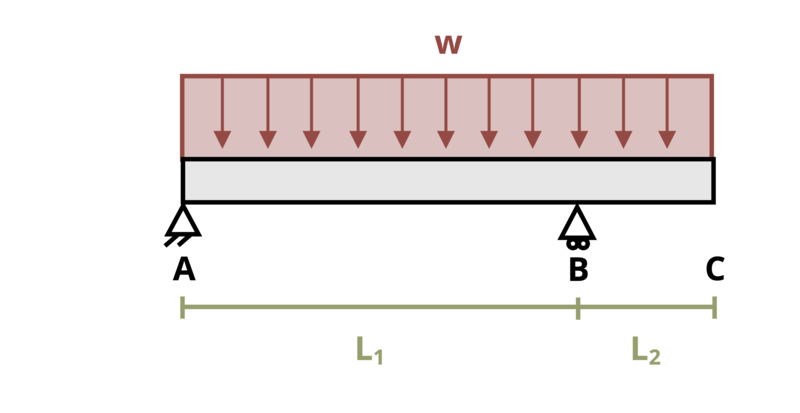
\includegraphics[keepaspectratio]{images/330.png}}
{[}Problem adapted from © Kurt Gramoll CC BY NC-SA 4.0{]}

\begin{Shaded}
\begin{Highlighting}[]
\NormalTok{\#| standalone: true}
\NormalTok{\#| viewerHeight: 600}
\NormalTok{\#| components: [viewer]}
\NormalTok{from shiny import App, render, ui, reactive}
\NormalTok{import random}
\NormalTok{import asyncio}
\NormalTok{import io}
\NormalTok{import math}
\NormalTok{import string}
\NormalTok{from datetime import datetime}
\NormalTok{from pathlib import Path}

\NormalTok{def generate\_random\_letters(length):}
\NormalTok{    \# Generate a random string of letters of specified length}
\NormalTok{    return \textquotesingle{}\textquotesingle{}.join(random.choice(string.ascii\_lowercase) for \_ in range(length))}

\NormalTok{problem\_ID="330"}
\NormalTok{w=reactive.Value("\_\_")}
\NormalTok{L1=reactive.Value("\_\_")}
\NormalTok{L2=reactive.Value("\_\_")}
\NormalTok{attempts=["Timestamp,Attempt,Answer,Feedback\textbackslash{}n"]}

\NormalTok{app\_ui = ui.page\_fluid(}
\NormalTok{    \#ui.markdown("**Please enter your ID number from your instructor and click to generate your problem**"),}
\NormalTok{    \#ui.input\_text("ID","", placeholder="Enter ID Number Here"),}
\NormalTok{    \#ui.input\_action\_button("generate\_problem", "Generate Problem", class\_="btn{-}primary"),}
\NormalTok{    ui.markdown("**Problem Statement**"),}
\NormalTok{    ui.output\_ui("ui\_problem\_statement"),}
\NormalTok{    ui.input\_text("answer1","Maximum absolute shear force in units of kN", placeholder="Please enter your answer 1"),}
\NormalTok{    ui.input\_text("answer2","Maximum absolute bending moment in units of kN{-}m", placeholder="Please enter your answer 2"),}
\NormalTok{    ui.input\_action\_button("submit", "Check Answers", class\_="btn{-}primary"),}
\NormalTok{    \#ui.download\_button("download", "Download File to Submit", class\_="btn{-}success"),}
\NormalTok{)}


\NormalTok{def server(input, output, session):}
\NormalTok{    \# Initialize a counter for attempts}
\NormalTok{    attempt\_counter = reactive.Value(0)}
    
\NormalTok{    @output}
\NormalTok{    @render.ui}
\NormalTok{    def ui\_problem\_statement():}
\NormalTok{        randomize\_vars()}
\NormalTok{        return[ui.markdown(f"Plot the shear force and bending moment diagrams for the loading shown. Assume w = \{w()\} kN/m, L\textless{}sub\textgreater{}1\textless{}/sub\textgreater{} = \{L1()\} m, and L\textless{}sub\textgreater{}2\textless{}/sub\textgreater{} = \{L2()\} m. What is the maximum absolute shear force and maximum absolute bending moment? ")]}
    
\NormalTok{    \#@reactive.Effect}
\NormalTok{    \#@reactive.event(input.generate\_problem)}
\NormalTok{    def randomize\_vars():}
\NormalTok{        random.seed(101)}
\NormalTok{        w.set(random.randrange(10, 75, 1))}
\NormalTok{        L2.set(random.randrange(10, 50, 1)/10)}
\NormalTok{        L1.set(round(L2()*3,1))}
\NormalTok{    @reactive.Effect}
\NormalTok{    @reactive.event(input.submit)}
\NormalTok{    def \_():}
\NormalTok{        attempt\_counter.set(attempt\_counter() + 1)}
\NormalTok{        instr1= abs((w()*(L1()+L2()){-}((L1()+L2())/2*w()*(L1()+L2()))/L1()){-}w()*L1())}
\NormalTok{        instr2 = abs((w()*(L1()+L2()){-}((L1()+L2())/2*w()*(L1()+L2()))/L1())**2/(2*w()))}
\NormalTok{        correct1 = math.isclose(float(input.answer1()), instr1, rel\_tol=0.01)}
\NormalTok{        correct2 = math.isclose(float(input.answer2()), instr2, rel\_tol=0.01)}
        
\NormalTok{        if correct1 and correct2:}
\NormalTok{            check = "both correct."}
\NormalTok{        else:}
\NormalTok{            check = f" \{\textquotesingle{}correct\textquotesingle{} if correct1 else \textquotesingle{}incorrect\textquotesingle{}\} and \{\textquotesingle{}correct respectively\textquotesingle{} if correct2 else \textquotesingle{}incorrect respectively\textquotesingle{}\}."}
        
\NormalTok{        correct\_indicator = "JL" if correct1 and correct2 else "JG"}

\NormalTok{        \# Generate random parts for the encoded attempt.}
\NormalTok{        random\_start = generate\_random\_letters(4)}
\NormalTok{        random\_middle = generate\_random\_letters(4)}
\NormalTok{        random\_end = generate\_random\_letters(4)}
\NormalTok{        \#encoded\_attempt = f"\{random\_start\}\{problem\_ID\}{-}\{random\_middle\}\{attempt\_counter()\}\{correct\_indicator\}{-}\{random\_end\}\{input.ID()\}"}

\NormalTok{        \# Store the most recent encoded attempt in a reactive value so it persists across submissions}
\NormalTok{        \#session.encoded\_attempt = reactive.Value(encoded\_attempt)}

\NormalTok{        \# Append the attempt data to the attempts list without the encoded attempt}
\NormalTok{        attempts.append(f"\{datetime.now()\}, \{attempt\_counter()\}, \{input.answer1()\}, \{input.answer2()\}, \{check\}\textbackslash{}n")}

\NormalTok{        \# Show feedback to the user.}
\NormalTok{        feedback = ui.markdown(f"Your answers of \{input.answer1()\} and \{input.answer2()\} are \{check\}.")}
\NormalTok{        m = ui.modal(feedback, title="Feedback", easy\_close=True)}
\NormalTok{        ui.modal\_show(m)}

\NormalTok{    \#@render.download(filename=lambda: f"Problem\_Log{-}\{problem\_ID\}{-}\{input.ID()\}.csv")}
\NormalTok{    async def download():}
\NormalTok{        \# Start the CSV with the encoded attempt (without label)}
\NormalTok{        final\_encoded = session.encoded\_attempt() if session.encoded\_attempt is not None else "No attempts"}
\NormalTok{        yield f"\{final\_encoded\}\textbackslash{}n\textbackslash{}n"}
        
\NormalTok{        \# Write the header for the remaining CSV data once}
\NormalTok{        yield "Timestamp,Attempt,Answer,Feedback\textbackslash{}n"}
        
\NormalTok{        \# Write the attempts data, ensure that the header from the attempts list is not written again}
\NormalTok{        for attempt in attempts[1:]:  \# Skip the first element which is the header}
\NormalTok{            await asyncio.sleep(0.25)  \# This delay may not be necessary; adjust as needed}
\NormalTok{            yield attempt}

\NormalTok{\# App installation}
\NormalTok{app = App(app\_ui, server)}
\end{Highlighting}
\end{Shaded}

\chapter*{Problem 7.27 - Graphical Methods for Shear Force \& Bending
Moment
Diagrams}\label{problem-7.27---graphical-methods-for-shear-force-bending-moment-diagrams}
\addcontentsline{toc}{chapter}{Problem 7.27 - Graphical Methods for
Shear Force \& Bending Moment Diagrams}

\markboth{Problem 7.27 - Graphical Methods for Shear Force \& Bending
Moment Diagrams}{Problem 7.27 - Graphical Methods for Shear Force \&
Bending Moment Diagrams}

\pandocbounded{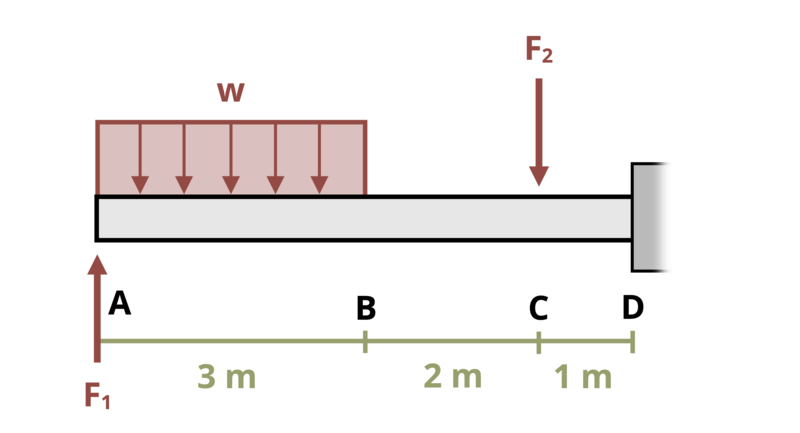
\includegraphics[keepaspectratio]{images/332.png}}
{[}Problem adapted from © Kurt Gramoll CC BY NC-SA 4.0{]}

\begin{Shaded}
\begin{Highlighting}[]
\NormalTok{\#| standalone: true}
\NormalTok{\#| viewerHeight: 600}
\NormalTok{\#| components: [viewer]}

\NormalTok{from shiny import App, render, ui, reactive}
\NormalTok{import random}
\NormalTok{import asyncio}
\NormalTok{import io}
\NormalTok{import math}
\NormalTok{import string}
\NormalTok{from datetime import datetime}
\NormalTok{from pathlib import Path}

\NormalTok{def generate\_random\_letters(length):}
\NormalTok{    \# Generate a random string of letters of specified length}
\NormalTok{    return \textquotesingle{}\textquotesingle{}.join(random.choice(string.ascii\_lowercase) for \_ in range(length))  }

\NormalTok{problem\_ID="332"}
\NormalTok{w=reactive.Value("\_\_")}
\NormalTok{F1=reactive.Value("\_\_")}
\NormalTok{F2=reactive.Value("\_\_")}
  
\NormalTok{attempts=["Timestamp,Attempt,Answer,Feedback\textbackslash{}n"]}

\NormalTok{app\_ui = ui.page\_fluid(}
\NormalTok{    \#ui.markdown("**Please enter your ID number from your instructor and click to generate your problem**"),}
\NormalTok{    \#ui.input\_text("ID","", placeholder="Enter ID Number Here"),}
\NormalTok{    \#ui.input\_action\_button("generate\_problem", "Generate Problem", class\_="btn{-}primary"),}
\NormalTok{    ui.markdown("**Problem Statement**"),}
\NormalTok{    ui.output\_ui("ui\_problem\_statement"),}
\NormalTok{    ui.input\_text("answer","Your Answer in units of m", placeholder="Please enter your answer"),}
\NormalTok{    ui.input\_action\_button("submit", "Check Answer", class\_="btn{-}primary"),}
\NormalTok{    \#ui.download\_button("download", "Download File to Submit", class\_="btn{-}success"),}
\NormalTok{)}

\NormalTok{def server(input, output, session):}
\NormalTok{    \# Initialize a counter for attempts}
\NormalTok{    attempt\_counter = reactive.Value(0)}

\NormalTok{    @output}
\NormalTok{    @render.ui}
\NormalTok{    def ui\_problem\_statement():}
\NormalTok{        randomize\_vars()}
\NormalTok{        return[ui.markdown(f"A beam is loaded as shown. Determine the distance from point A to where the internal shear force is zero. Assume w = \{w()\} kN/m, F\textless{}sub\textgreater{}1\textless{}/sub\textgreater{} = \{F1()\} kN, and F\textless{}sub\textgreater{}2\textless{}/sub\textgreater{} = \{F2()\} kN.")]}
    
\NormalTok{    \#@reactive.Effect}
\NormalTok{    \#@reactive.event(input.generate\_problem)}
\NormalTok{    def randomize\_vars():}
\NormalTok{        random.seed(101)}
\NormalTok{        w.set(random.randrange(2,10,1))}
\NormalTok{        F1.set(w()*random.randrange(15,25,1)/10)}
\NormalTok{        F2.set(random.randrange(5,25,1))}
        
\NormalTok{    @reactive.Effect}
\NormalTok{    @reactive.event(input.submit)}
\NormalTok{    def \_():}
\NormalTok{        attempt\_counter.set(attempt\_counter() + 1)  \# Increment the attempt counter on each submission.}
\NormalTok{        instr = F1()*3/(w()*3)}

\NormalTok{        if math.isclose(float(input.answer()), instr, rel\_tol=0.01):}
\NormalTok{            check = "*Correct*"}
\NormalTok{            correct\_indicator = "JL"}
\NormalTok{        else:}
\NormalTok{            check = "*Not Correct.*"}
\NormalTok{            correct\_indicator = "JG"}

\NormalTok{        \# Generate random parts for the encoded attempt.}
\NormalTok{        random\_start = generate\_random\_letters(4)}
\NormalTok{        random\_middle = generate\_random\_letters(4)}
\NormalTok{        random\_end = generate\_random\_letters(4)}
\NormalTok{        \#encoded\_attempt = f"\{random\_start\}\{problem\_ID\}{-}\{random\_middle\}\{attempt\_counter()\}\{correct\_indicator\}{-}\{random\_end\}\{input.ID()\}"}

\NormalTok{        \# Store the most recent encoded attempt in a reactive value so it persists across submissions}
\NormalTok{        \#session.encoded\_attempt = reactive.Value(encoded\_attempt)}

\NormalTok{        \# Append the attempt data to the attempts list without the encoded attempt}
\NormalTok{        attempts.append(f"\{datetime.now()\}, \{attempt\_counter()\}, \{input.answer()\}, \{check\}\textbackslash{}n")}

\NormalTok{        \# Show feedback to the user.}
\NormalTok{        feedback = ui.markdown(f"Your answer of \{input.answer()\} is \{check\}.")}
\NormalTok{        m = ui.modal(}
\NormalTok{            feedback,}
\NormalTok{            title="Feedback",}
\NormalTok{            easy\_close=True}
\NormalTok{        )}
\NormalTok{        ui.modal\_show(m)}

\NormalTok{    \#@render.download(filename=lambda: f"Problem\_Log{-}\{problem\_ID\}{-}\{input.ID()\}.csv")}
\NormalTok{    async def download():}
\NormalTok{        \# Start the CSV with the encoded attempt (without label)}
\NormalTok{        final\_encoded = session.encoded\_attempt() if session.encoded\_attempt is not None else "No attempts"}
\NormalTok{        yield f"\{final\_encoded\}\textbackslash{}n\textbackslash{}n"}
        
\NormalTok{        \# Write the header for the remaining CSV data once}
\NormalTok{        yield "Timestamp,Attempt,Answer,Feedback\textbackslash{}n"}
        
\NormalTok{        \# Write the attempts data, ensure that the header from the attempts list is not written again}
\NormalTok{        for attempt in attempts[1:]:  \# Skip the first element which is the header}
\NormalTok{            await asyncio.sleep(0.25)  \# This delay may not be necessary; adjust as needed}
\NormalTok{            yield attempt}

\NormalTok{\# App installation}
\NormalTok{app = App(app\_ui, server)}
\end{Highlighting}
\end{Shaded}

\chapter*{Problem 7.28 - Graphical Methods for Shear Force \& Bending
Moment
Diagrams}\label{problem-7.28---graphical-methods-for-shear-force-bending-moment-diagrams}
\addcontentsline{toc}{chapter}{Problem 7.28 - Graphical Methods for
Shear Force \& Bending Moment Diagrams}

\markboth{Problem 7.28 - Graphical Methods for Shear Force \& Bending
Moment Diagrams}{Problem 7.28 - Graphical Methods for Shear Force \&
Bending Moment Diagrams}

\pandocbounded{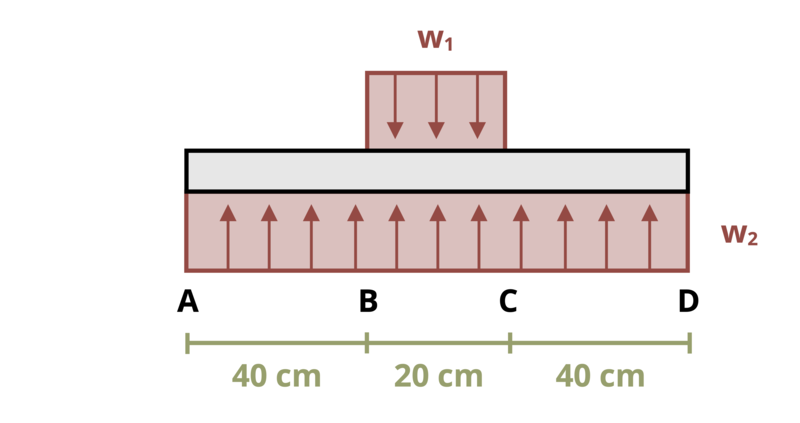
\includegraphics[keepaspectratio]{images/333.png}}
{[}Problem adapted from © Kurt Gramoll CC BY NC-SA 4.0{]}

\begin{Shaded}
\begin{Highlighting}[]
\NormalTok{\#| standalone: true}
\NormalTok{\#| viewerHeight: 600}
\NormalTok{\#| components: [viewer]}
\NormalTok{from shiny import App, render, ui, reactive}
\NormalTok{import random}
\NormalTok{import asyncio}
\NormalTok{import io}
\NormalTok{import math}
\NormalTok{import string}
\NormalTok{from datetime import datetime}
\NormalTok{from pathlib import Path}

\NormalTok{def generate\_random\_letters(length):}
\NormalTok{    \# Generate a random string of letters of specified length}
\NormalTok{    return \textquotesingle{}\textquotesingle{}.join(random.choice(string.ascii\_lowercase) for \_ in range(length))}

\NormalTok{problem\_ID="333"}
\NormalTok{w1=reactive.Value("\_\_")}
\NormalTok{w2=reactive.Value("\_\_")}
\NormalTok{attempts=["Timestamp,Attempt,Answer,Feedback\textbackslash{}n"]}

\NormalTok{app\_ui = ui.page\_fluid(}
\NormalTok{    \#ui.markdown("**Please enter your ID number from your instructor and click to generate your problem**"),}
\NormalTok{    \#ui.input\_text("ID","", placeholder="Enter ID Number Here"),}
\NormalTok{    \#ui.input\_action\_button("generate\_problem", "Generate Problem", class\_="btn{-}primary"),}
\NormalTok{    ui.markdown("**Problem Statement**"),}
\NormalTok{    ui.output\_ui("ui\_problem\_statement"),}
\NormalTok{    ui.input\_text("answer1","Maximum absolute shear force in units of kN", placeholder="Please enter your answer 1"),}
\NormalTok{    ui.input\_text("answer2","Maximum absolute bending moment in units of kN{-}m", placeholder="Please enter your answer 2"),}
\NormalTok{    ui.input\_action\_button("submit", "Check Answers", class\_="btn{-}primary"),}
\NormalTok{    \#ui.download\_button("download", "Download File to Submit", class\_="btn{-}success"),}
\NormalTok{)}

\NormalTok{def server(input, output, session):}
\NormalTok{    \# Initialize a counter for attempts}
\NormalTok{    attempt\_counter = reactive.Value(0)}
    
\NormalTok{    @output}
\NormalTok{    @render.ui}
\NormalTok{    def ui\_problem\_statement():}
\NormalTok{        randomize\_vars()}
\NormalTok{        return[ui.markdown(f"Plot the shear force and bending moment diagrams for the loading shown. Assume w\textless{}sub\textgreater{}1\textless{}/sub\textgreater{} = \{w1()\} kN/m, and w\textless{}sub\textgreater{}2\textless{}/sub\textgreater{} = \{w2()\} kN/m. What is the maximum absolute shear force and maximum absolute bending moment? ")]}
    
\NormalTok{    \#@reactive.Effect}
\NormalTok{    \#@reactive.event(input.generate\_problem)}
\NormalTok{    def randomize\_vars():}
\NormalTok{        random.seed(101)}
\NormalTok{        w2.set(random.randrange(10, 50, 1))}
\NormalTok{        w1.set(w2()*5)}
\NormalTok{    @reactive.Effect}
\NormalTok{    @reactive.event(input.submit)}
\NormalTok{    def \_():}
\NormalTok{        attempt\_counter.set(attempt\_counter() + 1)}
\NormalTok{        instr1= abs(0.4*w2())}
\NormalTok{        instr2 = abs(0.4*w2()*0.4*0.5 + 0.4*w2()*0.1*0.5)}
\NormalTok{        correct1 = math.isclose(float(input.answer1()), instr1, rel\_tol=0.01)}
\NormalTok{        correct2 = math.isclose(float(input.answer2()), instr2, rel\_tol=0.01)}
        
\NormalTok{        if correct1 and correct2:}
\NormalTok{            check = "both correct."}
\NormalTok{        elif correct1:}
\NormalTok{            check = f" \{\textquotesingle{}correct for answer 1 and incorrect for answer 2.\textquotesingle{}\}"}
\NormalTok{        elif correct2:}
\NormalTok{            check = f"\{\textquotesingle{}incorrect for answer 1 and correct for answer 2.\textquotesingle{}\}"}
\NormalTok{        else:}
\NormalTok{            check = f"\{\textquotesingle{}both incorrect.\textquotesingle{}\}"}
            
\NormalTok{        correct\_indicator = "JL" if correct1 and correct2 else "JG"}

\NormalTok{        \# Generate random parts for the encoded attempt.}
\NormalTok{        random\_start = generate\_random\_letters(4)}
\NormalTok{        random\_middle = generate\_random\_letters(4)}
\NormalTok{        random\_end = generate\_random\_letters(4)}
\NormalTok{        \#encoded\_attempt = f"\{random\_start\}\{problem\_ID\}{-}\{random\_middle\}\{attempt\_counter()\}\{correct\_indicator\}{-}\{random\_end\}\{input.ID()\}"}

\NormalTok{        \# Store the most recent encoded attempt in a reactive value so it persists across submissions}
\NormalTok{        \#session.encoded\_attempt = reactive.Value(encoded\_attempt)}

\NormalTok{        \# Append the attempt data to the attempts list without the encoded attempt}
\NormalTok{        attempts.append(f"\{datetime.now()\}, \{attempt\_counter()\}, \{input.answer1()\}, \{input.answer2()\}, \{check\}\textbackslash{}n")}

\NormalTok{        \# Show feedback to the user.}
\NormalTok{        feedback = ui.markdown(f"Your answers of \{input.answer1()\} and \{input.answer2()\} are \{check\}.")}
\NormalTok{        m = ui.modal(feedback, title="Feedback", easy\_close=True)}
\NormalTok{        ui.modal\_show(m)}

\NormalTok{    \#@render.download(filename=lambda: f"Problem\_Log{-}\{problem\_ID\}{-}\{input.ID()\}.csv")}
\NormalTok{    async def download():}
\NormalTok{        \# Start the CSV with the encoded attempt (without label)}
\NormalTok{        final\_encoded = session.encoded\_attempt() if session.encoded\_attempt is not None else "No attempts"}
\NormalTok{        yield f"\{final\_encoded\}\textbackslash{}n\textbackslash{}n"}
        
\NormalTok{        \# Write the header for the remaining CSV data once}
\NormalTok{        yield "Timestamp,Attempt,Answer,Feedback\textbackslash{}n"}
        
\NormalTok{        \# Write the attempts data, ensure that the header from the attempts list is not written again}
\NormalTok{        for attempt in attempts[1:]:  \# Skip the first element which is the header}
\NormalTok{            await asyncio.sleep(0.25)  \# This delay may not be necessary; adjust as needed}
\NormalTok{            yield attempt}

\NormalTok{\# App installation}
\NormalTok{app = App(app\_ui, server)}
\end{Highlighting}
\end{Shaded}

\chapter*{Problem 7.29 - Graphical Methods for Shear Force \& Bending
Moment
Diagrams}\label{problem-7.29---graphical-methods-for-shear-force-bending-moment-diagrams}
\addcontentsline{toc}{chapter}{Problem 7.29 - Graphical Methods for
Shear Force \& Bending Moment Diagrams}

\markboth{Problem 7.29 - Graphical Methods for Shear Force \& Bending
Moment Diagrams}{Problem 7.29 - Graphical Methods for Shear Force \&
Bending Moment Diagrams}

\pandocbounded{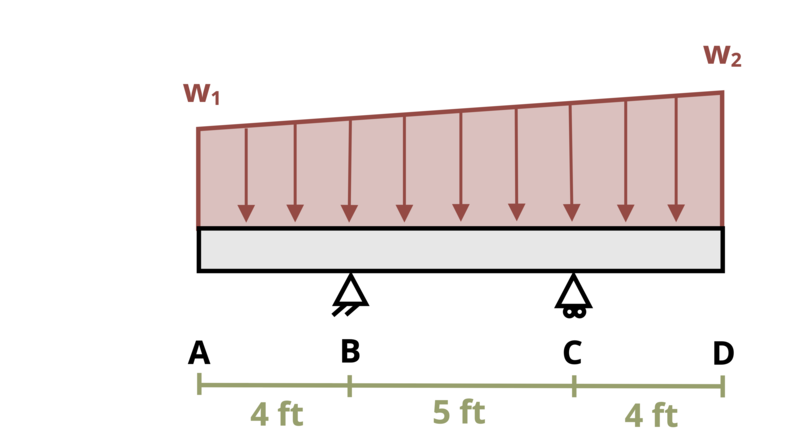
\includegraphics[keepaspectratio]{images/334.png}}
{[}Problem adapted from © Kurt Gramoll CC BY NC-SA 4.0{]}

\begin{Shaded}
\begin{Highlighting}[]
\NormalTok{\#| standalone: true}
\NormalTok{\#| viewerHeight: 600}
\NormalTok{\#| components: [viewer]}
\NormalTok{from shiny import App, render, ui, reactive}
\NormalTok{import random}
\NormalTok{import asyncio}
\NormalTok{import io}
\NormalTok{import math}
\NormalTok{import string}
\NormalTok{from datetime import datetime}
\NormalTok{from pathlib import Path}

\NormalTok{def generate\_random\_letters(length):}
\NormalTok{    \# Generate a random string of letters of specified length}
\NormalTok{    return \textquotesingle{}\textquotesingle{}.join(random.choice(string.ascii\_lowercase) for \_ in range(length))}

\NormalTok{problem\_ID="334"}
\NormalTok{w1=reactive.Value("\_\_")}
\NormalTok{w2=reactive.Value("\_\_")}
\NormalTok{attempts=["Timestamp,Attempt,Answer,Feedback\textbackslash{}n"]}

\NormalTok{app\_ui = ui.page\_fluid(}
\NormalTok{    \#ui.markdown("**Please enter your ID number from your instructor and click to generate your problem**"),}
\NormalTok{    \#ui.input\_text("ID","", placeholder="Enter ID Number Here"),}
\NormalTok{    \#ui.input\_action\_button("generate\_problem", "Generate Problem", class\_="btn{-}primary"),}
\NormalTok{    ui.markdown("**Problem Statement**"),}
\NormalTok{    ui.output\_ui("ui\_problem\_statement"),}
\NormalTok{    ui.input\_text("answer1","Maximum absolute shear force in units of kip", placeholder="Please enter your answer 1"),}
\NormalTok{    ui.input\_text("answer2","Maximum absolute bending moment in units of kip{-}ft", placeholder="Please enter your answer 2"),}
\NormalTok{    ui.input\_action\_button("submit", "Check Answers", class\_="btn{-}primary"),}
\NormalTok{    \#ui.download\_button("download", "Download File to Submit", class\_="btn{-}success"),}
\NormalTok{)}

\NormalTok{def server(input, output, session):}
\NormalTok{    \# Initialize a counter for attempts}
\NormalTok{    attempt\_counter = reactive.Value(0)}
    
\NormalTok{    @output}
\NormalTok{    @render.ui}
\NormalTok{    def ui\_problem\_statement():}
\NormalTok{        randomize\_vars()}
\NormalTok{        return[ui.markdown(f"Plot the shear force and bending moment diagrams for the loading shown. Assume w\textless{}sub\textgreater{}1\textless{}/sub\textgreater{} = \{w1()\} kip/ft and w\textless{}sub\textgreater{}2\textless{}/sub\textgreater{} = \{w2()\} kip/ft. What is the maximum absolute shear force and maximum absolute bending moment?")]}
    
\NormalTok{    \#@reactive.Effect}
\NormalTok{    \#@reactive.event(input.generate\_problem)}
\NormalTok{    def randomize\_vars():}
\NormalTok{        random.seed(101)}
\NormalTok{        w1.set(random.randrange(10, 300, 1)/10)}
\NormalTok{        w2.set(w1()*2)}
\NormalTok{    @reactive.Effect}
\NormalTok{    @reactive.event(input.submit)}
\NormalTok{    def \_():}
\NormalTok{        attempt\_counter.set(attempt\_counter() + 1)}
\NormalTok{        By = 13*(w2(){-}w1())/30+6.5*w1()}
\NormalTok{        Cy = 13*w1()+13*(w2(){-}w1())/2{-}By}
\NormalTok{     \#   instr1= abs(By+Cy{-}9*w1(){-}162/(13*(w2(){-}w1())))}
\NormalTok{     \#   instr2 = abs(5*By{-}81*w1()/2{-}486/(13*(w2(){-}w1())))}
\NormalTok{        instr1 = max(5.1854*w1(), Cy{-}5.1854*w1())}
\NormalTok{        instr2 = 15.17*w1()}
\NormalTok{        correct1 = math.isclose(float(input.answer1()), instr1, rel\_tol=0.01)}
\NormalTok{        correct2 = math.isclose(float(input.answer2()), instr2, rel\_tol=0.01)}
        
\NormalTok{        if correct1 and correct2:}
\NormalTok{            check = "both correct."}
\NormalTok{        else:}
\NormalTok{            check = f" \{\textquotesingle{}correct\textquotesingle{} if correct1 else \textquotesingle{}incorrect\textquotesingle{}\} and \{\textquotesingle{}correct respectively\textquotesingle{} if correct2 else \textquotesingle{}incorrect respectively\textquotesingle{}\}."}
        
\NormalTok{        correct\_indicator = "JL" if correct1 and correct2 else "JG"}

\NormalTok{        \# Generate random parts for the encoded attempt.}
\NormalTok{        random\_start = generate\_random\_letters(4)}
\NormalTok{        random\_middle = generate\_random\_letters(4)}
\NormalTok{        random\_end = generate\_random\_letters(4)}
\NormalTok{        \#encoded\_attempt = f"\{random\_start\}\{problem\_ID\}{-}\{random\_middle\}\{attempt\_counter()\}\{correct\_indicator\}{-}\{random\_end\}\{input.ID()\}"}

\NormalTok{        \# Store the most recent encoded attempt in a reactive value so it persists across submissions}
\NormalTok{        \#session.encoded\_attempt = reactive.Value(encoded\_attempt)}

\NormalTok{        \# Append the attempt data to the attempts list without the encoded attempt}
\NormalTok{        attempts.append(f"\{datetime.now()\}, \{attempt\_counter()\}, \{input.answer1()\}, \{input.answer2()\}, \{check\}\textbackslash{}n")}

\NormalTok{        \# Show feedback to the user.}
\NormalTok{        feedback = ui.markdown(f"Your answers of \{input.answer1()\} and \{input.answer2()\} are \{check\}.")}
\NormalTok{        m = ui.modal(feedback, title="Feedback", easy\_close=True)}
\NormalTok{        ui.modal\_show(m)}

\NormalTok{    \#@render.download(filename=lambda: f"Problem\_Log{-}\{problem\_ID\}{-}\{input.ID()\}.csv")}
\NormalTok{    async def download():}
\NormalTok{        \# Start the CSV with the encoded attempt (without label)}
\NormalTok{        final\_encoded = session.encoded\_attempt() if session.encoded\_attempt is not None else "No attempts"}
\NormalTok{        yield f"\{final\_encoded\}\textbackslash{}n\textbackslash{}n"}
        
\NormalTok{        \# Write the header for the remaining CSV data once}
\NormalTok{        yield "Timestamp,Attempt,Answer,Feedback\textbackslash{}n"}
        
\NormalTok{        \# Write the attempts data, ensure that the header from the attempts list is not written again}
\NormalTok{        for attempt in attempts[1:]:  \# Skip the first element which is the header}
\NormalTok{            await asyncio.sleep(0.25)  \# This delay may not be necessary; adjust as needed}
\NormalTok{            yield attempt}

\NormalTok{\# App installation}
\NormalTok{app = App(app\_ui, server)}
\end{Highlighting}
\end{Shaded}

\chapter*{Problem 7.30 - Graphical Methods for Shear Force \& Bending
Moment
Diagrams}\label{problem-7.30---graphical-methods-for-shear-force-bending-moment-diagrams}
\addcontentsline{toc}{chapter}{Problem 7.30 - Graphical Methods for
Shear Force \& Bending Moment Diagrams}

\markboth{Problem 7.30 - Graphical Methods for Shear Force \& Bending
Moment Diagrams}{Problem 7.30 - Graphical Methods for Shear Force \&
Bending Moment Diagrams}

\pandocbounded{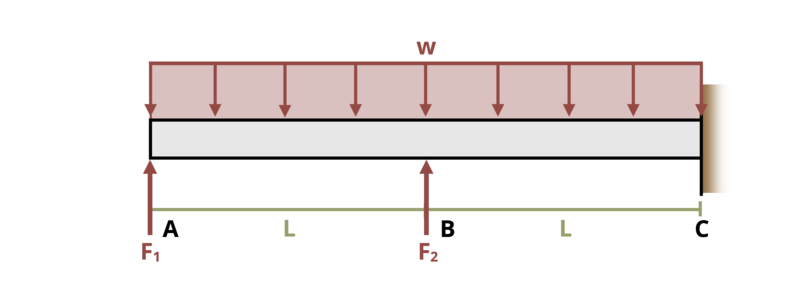
\includegraphics[keepaspectratio]{images/336.png}}
{[}Problem adapted from © Kurt Gramoll CC BY NC-SA 4.0{]}

\begin{Shaded}
\begin{Highlighting}[]
\NormalTok{\#| standalone: true}
\NormalTok{\#| viewerHeight: 600}
\NormalTok{\#| components: [viewer]}

\NormalTok{from shiny import App, render, ui, reactive}
\NormalTok{import random}
\NormalTok{import asyncio}
\NormalTok{import io}
\NormalTok{import math}
\NormalTok{import string}
\NormalTok{from datetime import datetime}
\NormalTok{from pathlib import Path}

\NormalTok{def generate\_random\_letters(length):}
\NormalTok{    \# Generate a random string of letters of specified length}
\NormalTok{    return "".join(random.choice(string.ascii\_lowercase) for \_ in range(length))}

\NormalTok{problem\_ID = "336"}
\NormalTok{w = reactive.Value("\_\_")}
\NormalTok{F1 = reactive.Value("\_\_")}
\NormalTok{F2 = reactive.Value("\_\_")}
\NormalTok{L = reactive.Value("\_\_")}
\NormalTok{attempts = ["Timestamp,Attempt,Answer1,Answer2,Feedback\textbackslash{}n"]}

\NormalTok{app\_ui = ui.page\_fluid(}
\NormalTok{    \#ui.markdown("**Please enter your ID number from your instructor and click to generate your problem**"),}
\NormalTok{    \#ui.input\_text("ID", "", placeholder="Enter ID Number Here"),}
\NormalTok{    \#ui.input\_action\_button("generate\_problem", "Generate Problem", class\_="btn{-}primary"),}
\NormalTok{    ui.markdown("**Problem Statement**"),}
\NormalTok{    ui.output\_ui("ui\_problem\_statement"),}
\NormalTok{    ui.input\_text("answer1", "Your Answer 1 in units of kip", placeholder="Please enter your answer 1"),}
\NormalTok{    ui.input\_text("answer2", "Your Answer 2 in units of kip{-}ft", placeholder="Please enter your answer 2"),}
\NormalTok{    ui.input\_action\_button("submit", "Check Answers", class\_="btn{-}primary"),}
\NormalTok{    \#ui.download\_button("download", "Download File to Submit", class\_="btn{-}success"),}
\NormalTok{)}

\NormalTok{def server(input, output, session):}
\NormalTok{    \# Initialize a counter for attempts}
\NormalTok{    attempt\_counter = reactive.Value(0)}

\NormalTok{    @output}
\NormalTok{    @render.ui}
\NormalTok{    def ui\_problem\_statement():}
\NormalTok{        randomize\_vars()}
\NormalTok{        return [}
\NormalTok{            ui.markdown(}
\NormalTok{                f"Plot the shear force and bending moment diagrams for the loading shown. Assume w = \{w()\} kip/ft, F\textless{}sub\textgreater{}1\textless{}/sub\textgreater{} = \{F1()\} kip, F\textless{}sub\textgreater{}2\textless{}/sub\textgreater{} = \{F2()\} kip, and L = \{L()\} ft. What is the maximum absolute shear force and maximum absolute bending moment?."}
\NormalTok{            )}
\NormalTok{        ]}

\NormalTok{    \#@reactive.Effect}
\NormalTok{    \#@reactive.event(input.generate\_problem)}
\NormalTok{    def randomize\_vars():}
\NormalTok{        random.seed(101)}
\NormalTok{        w.set(random.randrange(10,100,1)/10)}
\NormalTok{        F1.set(random.randrange(100,200,1)/10)}
\NormalTok{        F2.set(random.randrange(100,200,1)/10)}
\NormalTok{        L.set(random.randrange(20,50,1)/10)}
        
\NormalTok{    @reactive.Effect}
\NormalTok{    @reactive.event(input.submit)}
\NormalTok{    def \_():}
\NormalTok{        attempt\_counter.set(}
\NormalTok{            attempt\_counter() + 1}
\NormalTok{        )  \# Increment the attempt counter on each submission.}

\NormalTok{        \# Calculate the instructor\textquotesingle{}s answer and determine if the user\textquotesingle{}s answer is correct.}
\NormalTok{        instr1 = w()*2*L(){-}F1(){-}F2()}
\NormalTok{        instr2 = F1()*F1()/w(){-}w()/2*(F1()/w())**2}

\NormalTok{        correct1 = math.isclose(float(input.answer1()), instr1, rel\_tol=0.01)}
\NormalTok{        correct2 = math.isclose(float(input.answer2()), instr2, rel\_tol=0.01)}
        
\NormalTok{        if correct1 and correct2:}
\NormalTok{            check = f"\{\textquotesingle{}both correct.\textquotesingle{}\}"}
\NormalTok{        elif correct1:}
\NormalTok{            check = f" \{\textquotesingle{}correct for answer 1 and incorrect for answer 2.\textquotesingle{}\}"}
\NormalTok{        elif correct2:}
\NormalTok{            check = f"\{\textquotesingle{}incorrect for answer 1 and correct for answer 2.\textquotesingle{}\}"}
\NormalTok{        else:}
\NormalTok{            check = f"\{\textquotesingle{}both incorrect.\textquotesingle{}\}"}
        
\NormalTok{        correct\_indicator = "JL" if correct1 and correct2 else "JG"}

\NormalTok{        random\_start = generate\_random\_letters(4)}
\NormalTok{        random\_middle = generate\_random\_letters(4)}
\NormalTok{        random\_end = generate\_random\_letters(4)}
\NormalTok{        \#encoded\_attempt = f"\{random\_start\}\{problem\_ID\}{-}\{random\_middle\}\{attempt\_counter()\}\{correct\_indicator\}{-}\{random\_end\}\{input.ID()\}"}

\NormalTok{        \#session.encoded\_attempt = reactive.Value(encoded\_attempt)}
\NormalTok{        attempts.append(f"\{datetime.now()\}, \{attempt\_counter()\}, \{input.answer1()\}, \{input.answer2()\}, \{check\}\textbackslash{}n")}

\NormalTok{        feedback = ui.markdown(f"Your answers of \{input.answer1()\} and \{input.answer2()\} are \{check\}.")}
\NormalTok{        m = ui.modal(feedback, title="Feedback", easy\_close=True)}
\NormalTok{        ui.modal\_show(m)}

\NormalTok{    \#@render.download(filename=lambda: f"Problem\_Log{-}\{problem\_ID\}{-}\{input.ID()\}.csv")}
\NormalTok{    async def download():}
\NormalTok{        final\_encoded = session.encoded\_attempt() if session.encoded\_attempt is not None else "No attempts"}
\NormalTok{        yield f"\{final\_encoded\}\textbackslash{}n\textbackslash{}n"}
\NormalTok{        yield "Timestamp,Attempt,Answer1,Answer2,Feedback\textbackslash{}n"}
\NormalTok{        for attempt in attempts[1:]:}
\NormalTok{            await asyncio.sleep(0.25)}
\NormalTok{            yield attempt}

\NormalTok{app = App(app\_ui, server)}
\end{Highlighting}
\end{Shaded}

\chapter*{Problem 7.31 - Graphical methods for shear force \& bending
moment
diagrams}\label{problem-7.31---graphical-methods-for-shear-force-bending-moment-diagrams}
\addcontentsline{toc}{chapter}{Problem 7.31 - Graphical methods for
shear force \& bending moment diagrams}

\markboth{Problem 7.31 - Graphical methods for shear force \& bending
moment diagrams}{Problem 7.31 - Graphical methods for shear force \&
bending moment diagrams}

\pandocbounded{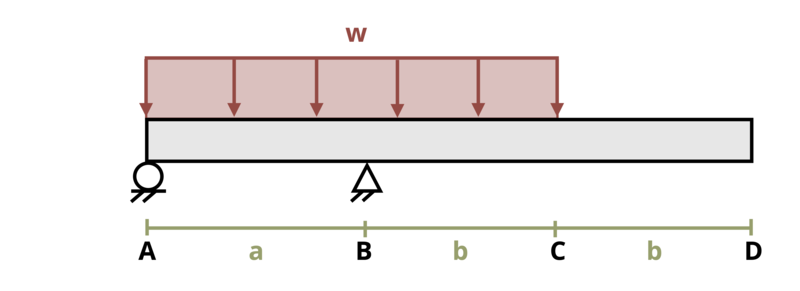
\includegraphics[keepaspectratio]{images/337.png}}\{fig-alt=''
A beam of length a+2b is subjected to a distributed load, w, over a
distance a. The beam has pin supports a distance of a, and a+b from the
left end of the beam. ``\} {[}Problem adapted from © Kurt Gramoll CC BY
NC-SA 4.0{]}

\begin{Shaded}
\begin{Highlighting}[]
\NormalTok{\#| standalone: true}
\NormalTok{\#| viewerHeight: 600}
\NormalTok{\#| components: [viewer]}

\NormalTok{from shiny import App, render, ui, reactive}
\NormalTok{import random}
\NormalTok{import asyncio}
\NormalTok{import io}
\NormalTok{import math}
\NormalTok{import string}
\NormalTok{from datetime import datetime}
\NormalTok{from pathlib import Path}

\NormalTok{def generate\_random\_letters(length):}
\NormalTok{    \# Generate a random string of letters of specified length}
\NormalTok{    return "".join(random.choice(string.ascii\_lowercase) for \_ in range(length))}

\NormalTok{problem\_ID = "337"}
\NormalTok{w = reactive.Value("\_\_")}
\NormalTok{b = reactive.Value("\_\_")}
\NormalTok{a = reactive.Value("\_\_")}
\NormalTok{attempts = ["Timestamp,Attempt,Answer1,Answer2,Feedback\textbackslash{}n"]}

\NormalTok{app\_ui = ui.page\_fluid(}
\NormalTok{    \#ui.markdown("**Please enter your ID number from your instructor and click to generate your problem**"),}
\NormalTok{    \#ui.input\_text("ID", "", placeholder="Enter ID Number Here"),}
\NormalTok{    \#ui.input\_action\_button("generate\_problem", "Generate Problem", class\_="btn{-}primary"),}
\NormalTok{    ui.markdown("**Problem Statement**"),}
\NormalTok{    ui.output\_ui("ui\_problem\_statement"),}
\NormalTok{    ui.input\_text("answer1", "Your Answer 1 in units of kN", placeholder="Please enter your answer 1"),}
\NormalTok{    ui.input\_text("answer2", "Your Answer 2 in units of kN{-}m", placeholder="Please enter your answer 2"),}
\NormalTok{    ui.input\_action\_button("submit", "Check Answers", class\_="btn{-}primary"),}
\NormalTok{    \#ui.download\_button("download", "Download File to Submit", class\_="btn{-}success"),}
\NormalTok{)}

\NormalTok{def server(input, output, session):}
\NormalTok{    \# Initialize a counter for attempts}
\NormalTok{    attempt\_counter = reactive.Value(0)}

\NormalTok{    @output}
\NormalTok{    @render.ui}
\NormalTok{    def ui\_problem\_statement():}
\NormalTok{        randomize\_vars()}
\NormalTok{        return [}
\NormalTok{            ui.markdown(}
\NormalTok{                f"Plot the shear force and bending moment diagrams for the loading shown. Assume w = \{w()\} kN/m, a = \{a()\} m, and b = \{b()\} m. What is the maximum absolute shear force and maximum absolute bending moment?"}
\NormalTok{            )}
\NormalTok{        ]}

\NormalTok{    \#@reactive.Effect}
\NormalTok{    \#@reactive.event(input.generate\_problem)}
\NormalTok{    def randomize\_vars():}
\NormalTok{        random.seed(101)}
\NormalTok{        w.set(random.randrange(10,100,1)/10)}
\NormalTok{        b.set(random.randrange(50,100,1)/10)}
\NormalTok{        a.set(b()+round(random.randrange(10,20,1)/10))}
        
\NormalTok{    @reactive.Effect}
\NormalTok{    @reactive.event(input.submit)}
\NormalTok{    def \_():}
\NormalTok{        attempt\_counter.set(}
\NormalTok{            attempt\_counter() + 1}
\NormalTok{        )  \# Increment the attempt counter on each submission.}

\NormalTok{        \# Calculate the instructor\textquotesingle{}s answer and determine if the user\textquotesingle{}s answer is correct.}
\NormalTok{        FB = w()*(a()+b())*(a()+b())/2/a()}
\NormalTok{        FA = FB{-}w()*(a()+b())}
\NormalTok{        instr1 = max(abs(FA{-}w()*a()),FA{-}w()*a()+FB)}
\NormalTok{        instr2 = abs(FA*a(){-}w()*a()**2/2)}

\NormalTok{        correct1 = math.isclose(float(input.answer1()), instr1, rel\_tol=0.01)}
\NormalTok{        correct2 = math.isclose(float(input.answer2()), instr2, rel\_tol=0.01)}
        
\NormalTok{        if correct1 and correct2:}
\NormalTok{            check = f"\{\textquotesingle{}both correct.\textquotesingle{}\}"}
\NormalTok{        elif correct1:}
\NormalTok{            check = f" \{\textquotesingle{}correct for answer 1 and incorrect for answer 2.\textquotesingle{}\}"}
\NormalTok{        elif correct2:}
\NormalTok{            check = f"\{\textquotesingle{}incorrect for answer 1 and correct for answer 2.\textquotesingle{}\}"}
\NormalTok{        else:}
\NormalTok{            check = f"\{\textquotesingle{}both incorrect.\textquotesingle{}\}"}
        
\NormalTok{        correct\_indicator = "JL" if correct1 and correct2 else "JG"}

\NormalTok{        random\_start = generate\_random\_letters(4)}
\NormalTok{        random\_middle = generate\_random\_letters(4)}
\NormalTok{        random\_end = generate\_random\_letters(4)}
\NormalTok{        \#encoded\_attempt = f"\{random\_start\}\{problem\_ID\}{-}\{random\_middle\}\{attempt\_counter()\}\{correct\_indicator\}{-}\{random\_end\}\{input.ID()\}"}

\NormalTok{        \#session.encoded\_attempt = reactive.Value(encoded\_attempt)}
\NormalTok{        attempts.append(f"\{datetime.now()\}, \{attempt\_counter()\}, \{input.answer1()\}, \{input.answer2()\}, \{check\}\textbackslash{}n")}

\NormalTok{        feedback = ui.markdown(f"Your answers of \{input.answer1()\} and \{input.answer2()\} are \{check\}.")}
\NormalTok{        m = ui.modal(feedback, title="Feedback", easy\_close=True)}
\NormalTok{        ui.modal\_show(m)}

\NormalTok{    \#@render.download(filename=lambda: f"Problem\_Log{-}\{problem\_ID\}{-}\{input.ID()\}.csv")}
\NormalTok{    async def download():}
\NormalTok{        final\_encoded = session.encoded\_attempt() if session.encoded\_attempt is not None else "No attempts"}
\NormalTok{        yield f"\{final\_encoded\}\textbackslash{}n\textbackslash{}n"}
\NormalTok{        yield "Timestamp,Attempt,Answer1,Answer2,Feedback\textbackslash{}n"}
\NormalTok{        for attempt in attempts[1:]:}
\NormalTok{            await asyncio.sleep(0.25)}
\NormalTok{            yield attempt}

\NormalTok{app = App(app\_ui, server)}
\end{Highlighting}
\end{Shaded}

\chapter*{Problem 7.32 - Graphical methods for shear force \& bending
moment
diagrams}\label{problem-7.32---graphical-methods-for-shear-force-bending-moment-diagrams}
\addcontentsline{toc}{chapter}{Problem 7.32 - Graphical methods for
shear force \& bending moment diagrams}

\markboth{Problem 7.32 - Graphical methods for shear force \& bending
moment diagrams}{Problem 7.32 - Graphical methods for shear force \&
bending moment diagrams}

\pandocbounded{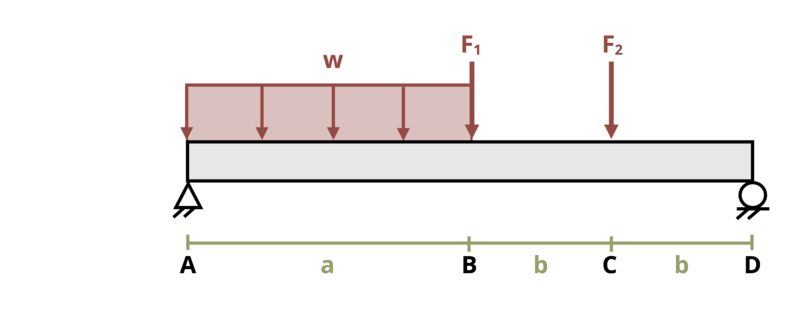
\includegraphics[keepaspectratio]{images/338.png}}
{[}Problem adapted from © Kurt Gramoll CC BY NC-SA 4.0{]}

\begin{Shaded}
\begin{Highlighting}[]
\NormalTok{\#| standalone: true}
\NormalTok{\#| viewerHeight: 600}
\NormalTok{\#| components: [viewer]}

\NormalTok{from shiny import App, render, ui, reactive}
\NormalTok{import random}
\NormalTok{import asyncio}
\NormalTok{import io}
\NormalTok{import math}
\NormalTok{import string}
\NormalTok{from datetime import datetime}
\NormalTok{from pathlib import Path}

\NormalTok{def generate\_random\_letters(length):}
\NormalTok{    \# Generate a random string of letters of specified length}
\NormalTok{    return "".join(random.choice(string.ascii\_lowercase) for \_ in range(length))}

\NormalTok{problem\_ID = "338"}
\NormalTok{w = reactive.Value("\_\_")}
\NormalTok{F1 = reactive.Value("\_\_")}
\NormalTok{F2 = reactive.Value("\_\_")}
\NormalTok{b = reactive.Value("\_\_")}
\NormalTok{a = reactive.Value("\_\_")}
\NormalTok{attempts = ["Timestamp,Attempt,Answer1,Answer2,Feedback\textbackslash{}n"]}

\NormalTok{app\_ui = ui.page\_fluid(}
\NormalTok{    \#ui.markdown("**Please enter your ID number from your instructor and click to generate your problem**"),}
\NormalTok{    \#ui.input\_text("ID", "", placeholder="Enter ID Number Here"),}
\NormalTok{    \#ui.input\_action\_button("generate\_problem", "Generate Problem", class\_="btn{-}primary"),}
\NormalTok{    ui.markdown("**Problem Statement**"),}
\NormalTok{    ui.output\_ui("ui\_problem\_statement"),}
\NormalTok{    ui.input\_text("answer1", "Your Answer 1 in units of lb", placeholder="Please enter your answer 1"),}
\NormalTok{    ui.input\_text("answer2", "Your Answer 2 in units of lb{-}ft", placeholder="Please enter your answer 2"),}
\NormalTok{    ui.input\_action\_button("submit", "Check Answers", class\_="btn{-}primary"),}
\NormalTok{    \#ui.download\_button("download", "Download File to Submit", class\_="btn{-}success"),}
\NormalTok{)}

\NormalTok{def server(input, output, session):}
\NormalTok{    \# Initialize a counter for attempts}
\NormalTok{    attempt\_counter = reactive.Value(0)}

\NormalTok{    @output}
\NormalTok{    @render.ui}
\NormalTok{    def ui\_problem\_statement():}
\NormalTok{        randomize\_vars()}
\NormalTok{        return [}
\NormalTok{            ui.markdown(}
\NormalTok{                f"Plot the shear force and bending moment diagrams for the loading shown. Assume w = \{w()\} lb/ft, F\textless{}sub\textgreater{}1\textless{}/sub\textgreater{} = \{F1()\} lb, F\textless{}sub\textgreater{}2\textless{}/sub\textgreater{} = \{F2()\} lb, a = \{a()\} ft, and b = \{b()\} ft. What is the maximum absolute shear force and maximum absolute bending moment?"}
\NormalTok{            )}
\NormalTok{        ]}

\NormalTok{    \#@reactive.Effect}
\NormalTok{    \#@reactive.event(input.generate\_problem)}
\NormalTok{    def randomize\_vars():}
\NormalTok{        random.seed(101)}
\NormalTok{        w.set(random.randrange(100,300,5))}
\NormalTok{        F1.set(random.randrange(500,1000,10))}
\NormalTok{        F2.set(random.randrange(500,1000,10))}
\NormalTok{        b.set(random.randrange(20,50,1)/10)}
\NormalTok{        a.set(b()+round(random.randrange(10,20,1)/10))}
        
\NormalTok{    @reactive.Effect}
\NormalTok{    @reactive.event(input.submit)}
\NormalTok{    def \_():}
\NormalTok{        attempt\_counter.set(}
\NormalTok{            attempt\_counter() + 1}
\NormalTok{        )  \# Increment the attempt counter on each submission.}

\NormalTok{        \# Calculate the instructor\textquotesingle{}s answer and determine if the user\textquotesingle{}s answer is correct.}
\NormalTok{        RD = (w()*a()*a()/2+F1()*a()+F2()*(a()+b()))/(a()+2*b())}
\NormalTok{        RA = (w()*a()*(2*b()+a()/2)+F1()*2*b()+F2()*b())/(a()+2*b())}
\NormalTok{        instr1 = max(RD,RA)}
\NormalTok{        instr2 = RA*a(){-}w()*a()*a()/2}

\NormalTok{        correct1 = math.isclose(float(input.answer1()), instr1, rel\_tol=0.01)}
\NormalTok{        correct2 = math.isclose(float(input.answer2()), instr2, rel\_tol=0.01)}
        
\NormalTok{        if correct1 and correct2:}
\NormalTok{            check = f"\{\textquotesingle{}both correct.\textquotesingle{}\}"}
\NormalTok{        elif correct1:}
\NormalTok{            check = f" \{\textquotesingle{}correct for answer 1 and incorrect for answer 2.\textquotesingle{}\}"}
\NormalTok{        elif correct2:}
\NormalTok{            check = f"\{\textquotesingle{}incorrect for answer 1 and correct for answer 2.\textquotesingle{}\}"}
\NormalTok{        else:}
\NormalTok{            check = f"\{\textquotesingle{}both incorrect.\textquotesingle{}\}"}
        
\NormalTok{        correct\_indicator = "JL" if correct1 and correct2 else "JG"}

\NormalTok{        random\_start = generate\_random\_letters(4)}
\NormalTok{        random\_middle = generate\_random\_letters(4)}
\NormalTok{        random\_end = generate\_random\_letters(4)}
\NormalTok{        \#encoded\_attempt = f"\{random\_start\}\{problem\_ID\}{-}\{random\_middle\}\{attempt\_counter()\}\{correct\_indicator\}{-}\{random\_end\}\{input.ID()\}"}

\NormalTok{        \#session.encoded\_attempt = reactive.Value(encoded\_attempt)}
\NormalTok{        attempts.append(f"\{datetime.now()\}, \{attempt\_counter()\}, \{input.answer1()\}, \{input.answer2()\}, \{check\}\textbackslash{}n")}

\NormalTok{        feedback = ui.markdown(f"Your answers of \{input.answer1()\} and \{input.answer2()\} are \{check\}.")}
\NormalTok{        m = ui.modal(feedback, title="Feedback", easy\_close=True)}
\NormalTok{        ui.modal\_show(m)}

\NormalTok{    \#@render.download(filename=lambda: f"Problem\_Log{-}\{problem\_ID\}{-}\{input.ID()\}.csv")}
\NormalTok{    async def download():}
\NormalTok{        final\_encoded = session.encoded\_attempt() if session.encoded\_attempt is not None else "No attempts"}
\NormalTok{        yield f"\{final\_encoded\}\textbackslash{}n\textbackslash{}n"}
\NormalTok{        yield "Timestamp,Attempt,Answer1,Answer2,Feedback\textbackslash{}n"}
\NormalTok{        for attempt in attempts[1:]:}
\NormalTok{            await asyncio.sleep(0.25)}
\NormalTok{            yield attempt}

\NormalTok{app = App(app\_ui, server)}
\end{Highlighting}
\end{Shaded}

\chapter*{Problem 7.33 - Graphical methods for shear force \& bending
moment
diagrams}\label{problem-7.33---graphical-methods-for-shear-force-bending-moment-diagrams}
\addcontentsline{toc}{chapter}{Problem 7.33 - Graphical methods for
shear force \& bending moment diagrams}

\markboth{Problem 7.33 - Graphical methods for shear force \& bending
moment diagrams}{Problem 7.33 - Graphical methods for shear force \&
bending moment diagrams}

\pandocbounded{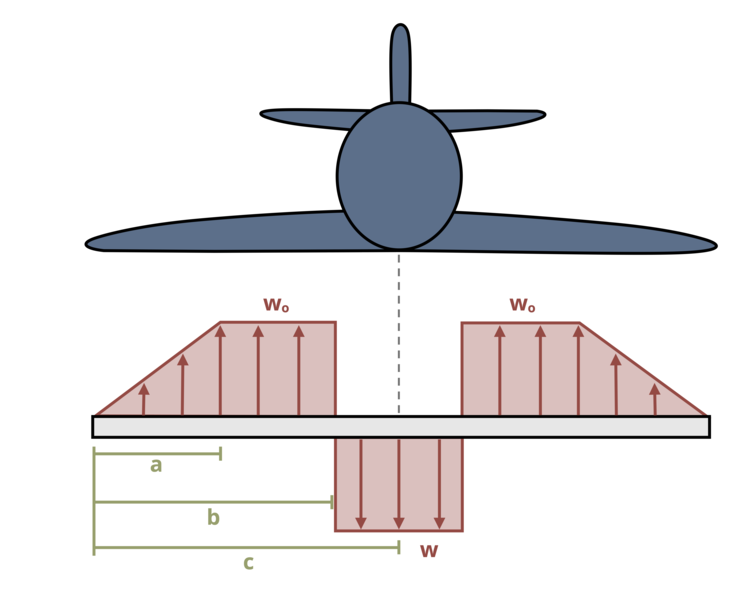
\includegraphics[keepaspectratio]{images/340.png}}
{[}Problem adapted from © Kurt Gramoll CC BY NC-SA 4.0{]}

\begin{Shaded}
\begin{Highlighting}[]
\NormalTok{\#| standalone: true}
\NormalTok{\#| viewerHeight: 600}
\NormalTok{\#| components: [viewer]}

\NormalTok{from shiny import App, render, ui, reactive}
\NormalTok{import random}
\NormalTok{import asyncio}
\NormalTok{import io}
\NormalTok{import math}
\NormalTok{import string}
\NormalTok{from datetime import datetime}
\NormalTok{from pathlib import Path}

\NormalTok{def generate\_random\_letters(length):}
\NormalTok{    \# Generate a random string of letters of specified length}
\NormalTok{    return "".join(random.choice(string.ascii\_lowercase) for \_ in range(length))}

\NormalTok{problem\_ID = "340"}
\NormalTok{w0 = reactive.Value("\_\_")}
\NormalTok{a = reactive.Value("\_\_")}
\NormalTok{b = reactive.Value("\_\_")}
\NormalTok{c = reactive.Value("\_\_")}
\NormalTok{attempts = ["Timestamp,Attempt,Answer1,Answer2,Feedback\textbackslash{}n"]}

\NormalTok{app\_ui = ui.page\_fluid(}
\NormalTok{    \#ui.markdown("**Please enter your ID number from your instructor and click to generate your problem**"),}
\NormalTok{    \#ui.input\_text("ID", "", placeholder="Enter ID Number Here"),}
\NormalTok{    \#ui.input\_action\_button("generate\_problem", "Generate Problem", class\_="btn{-}primary"),}
\NormalTok{    ui.markdown("**Problem Statement**"),}
\NormalTok{    ui.output\_ui("ui\_problem\_statement"),}
\NormalTok{    ui.input\_text("answer1", "Your Answer 1 in units of kip", placeholder="Please enter your answer 1"),}
\NormalTok{    ui.input\_text("answer2", "Your Answer 2 in units of kip{-}in", placeholder="Please enter your answer 2"),}
\NormalTok{    ui.input\_action\_button("submit", "Check Answers", class\_="btn{-}primary"),}
\NormalTok{    \#ui.download\_button("download", "Download File to Submit", class\_="btn{-}success"),}
\NormalTok{)}

\NormalTok{def server(input, output, session):}
\NormalTok{    \# Initialize a counter for attempts}
\NormalTok{    attempt\_counter = reactive.Value(0)}

\NormalTok{    @output}
\NormalTok{    @render.ui}
\NormalTok{    def ui\_problem\_statement():}
\NormalTok{        randomize\_vars()}
\NormalTok{        return [}
\NormalTok{            ui.markdown(}
\NormalTok{                f"The lift of an aircraft can be modeled as a beam with distributed loads as shown, where w\textless{}sub\textgreater{}0\textless{}/sub\textgreater{} = \{w0()\} lb/in. The aircraft weight is modeled as a uniform distributed load about the center of magnitude w. Assuming the lift distribution is symmetric around the center and that the plane is in static equilibrium, plot the shear force and bending moment diagrams for the loading shown. What is the maximum absolute shear force and maximum absolute bending moment? Assume lengths a = \{a()\} in., b = \{b()\} in., and c = \{c()\} in."}
\NormalTok{            )}
\NormalTok{        ]}

\NormalTok{    \#@reactive.Effect}
\NormalTok{    \#@reactive.event(input.generate\_problem)}
\NormalTok{    def randomize\_vars():}
\NormalTok{        random.seed(101)}
\NormalTok{        w0.set(random.randrange(50,100,1))}
\NormalTok{        a.set(random.randrange(80,120,1))}
\NormalTok{        b.set(a()+random.randrange(50,100,1))}
\NormalTok{        c.set(b()+random.randrange(10,20,1))}
        
\NormalTok{    @reactive.Effect}
\NormalTok{    @reactive.event(input.submit)}
\NormalTok{    def \_():}
\NormalTok{        attempt\_counter.set(}
\NormalTok{            attempt\_counter() + 1}
\NormalTok{        )  \# Increment the attempt counter on each submission.}

\NormalTok{        \# Calculate the instructor\textquotesingle{}s answer and determine if the user\textquotesingle{}s answer is correct.}
\NormalTok{        instr1 = (w0()*0.5*a()+w0()*(b(){-}a()))/1000}
\NormalTok{        instr2 = (w0()*b()**2/4+w0()*a()*b()/2)/1000}

\NormalTok{        correct1 = math.isclose(float(input.answer1()), instr1, rel\_tol=0.01)}
\NormalTok{        correct2 = math.isclose(float(input.answer2()), instr2, rel\_tol=0.01)}
        
\NormalTok{        if correct1 and correct2:}
\NormalTok{            check = f"\{\textquotesingle{}both correct.\textquotesingle{}\}"}
\NormalTok{        elif correct1:}
\NormalTok{            check = f" \{\textquotesingle{}correct for answer 1 and incorrect for answer 2.\textquotesingle{}\}"}
\NormalTok{        elif correct2:}
\NormalTok{            check = f"\{\textquotesingle{}incorrect for answer 1 and correct for answer 2.\textquotesingle{}\}"}
\NormalTok{        else:}
\NormalTok{            check = f"\{\textquotesingle{}both incorrect.\textquotesingle{}\}"}
        
\NormalTok{        correct\_indicator = "JL" if correct1 and correct2 else "JG"}

\NormalTok{        random\_start = generate\_random\_letters(4)}
\NormalTok{        random\_middle = generate\_random\_letters(4)}
\NormalTok{        random\_end = generate\_random\_letters(4)}
\NormalTok{        \#encoded\_attempt = f"\{random\_start\}\{problem\_ID\}{-}\{random\_middle\}\{attempt\_counter()\}\{correct\_indicator\}{-}\{random\_end\}\{input.ID()\}"}

\NormalTok{        \#session.encoded\_attempt = reactive.Value(encoded\_attempt)}
\NormalTok{        attempts.append(f"\{datetime.now()\}, \{attempt\_counter()\}, \{input.answer1()\}, \{input.answer2()\}, \{check\}\textbackslash{}n")}

\NormalTok{        feedback = ui.markdown(f"Your answers of \{input.answer1()\} and \{input.answer2()\} are \{check\}.")}
\NormalTok{        m = ui.modal(feedback, title="Feedback", easy\_close=True)}
\NormalTok{        ui.modal\_show(m)}

\NormalTok{    \#@render.download(filename=lambda: f"Problem\_Log{-}\{problem\_ID\}{-}\{input.ID()\}.csv")}
\NormalTok{    async def download():}
\NormalTok{        final\_encoded = session.encoded\_attempt() if session.encoded\_attempt is not None else "No attempts"}
\NormalTok{        yield f"\{final\_encoded\}\textbackslash{}n\textbackslash{}n"}
\NormalTok{        yield "Timestamp,Attempt,Answer1,Answer2,Feedback\textbackslash{}n"}
\NormalTok{        for attempt in attempts[1:]:}
\NormalTok{            await asyncio.sleep(0.25)}
\NormalTok{            yield attempt}

\NormalTok{app = App(app\_ui, server)}
\end{Highlighting}
\end{Shaded}

\chapter*{Problem 7.34 - Graphical methods for shear force \& bending
moment
diagrams}\label{problem-7.34---graphical-methods-for-shear-force-bending-moment-diagrams}
\addcontentsline{toc}{chapter}{Problem 7.34 - Graphical methods for
shear force \& bending moment diagrams}

\markboth{Problem 7.34 - Graphical methods for shear force \& bending
moment diagrams}{Problem 7.34 - Graphical methods for shear force \&
bending moment diagrams}

\pandocbounded{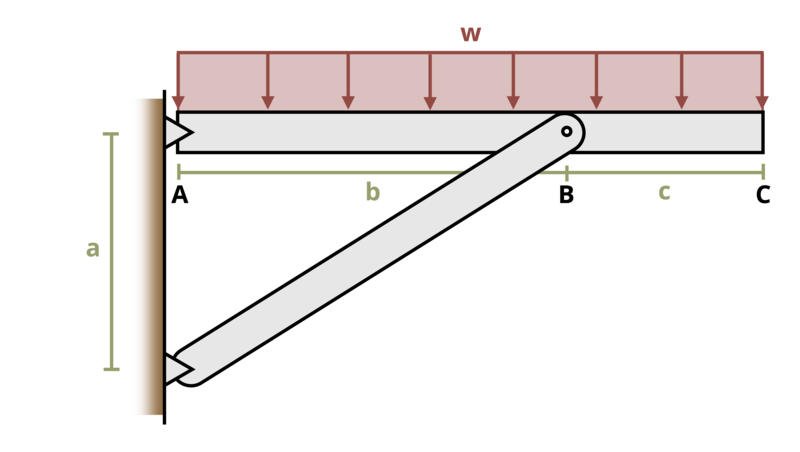
\includegraphics[keepaspectratio]{images/341.png}}
{[}Problem adapted from © Kurt Gramoll CC BY NC-SA 4.0{]}

\begin{Shaded}
\begin{Highlighting}[]
\NormalTok{\#| standalone: true}
\NormalTok{\#| viewerHeight: 600}
\NormalTok{\#| components: [viewer]}

\NormalTok{from shiny import App, render, ui, reactive}
\NormalTok{import random}
\NormalTok{import asyncio}
\NormalTok{import io}
\NormalTok{import math}
\NormalTok{import string}
\NormalTok{from datetime import datetime}
\NormalTok{from pathlib import Path}

\NormalTok{def generate\_random\_letters(length):}
\NormalTok{    \# Generate a random string of letters of specified length}
\NormalTok{    return "".join(random.choice(string.ascii\_lowercase) for \_ in range(length))}

\NormalTok{problem\_ID = "341"}
\NormalTok{w = reactive.Value("\_\_")}
\NormalTok{a = reactive.Value("\_\_")}
\NormalTok{b = reactive.Value("\_\_")}
\NormalTok{c = reactive.Value("\_\_")}
\NormalTok{attempts = ["Timestamp,Attempt,Answer1,Answer2,Feedback\textbackslash{}n"]}

\NormalTok{app\_ui = ui.page\_fluid(}
\NormalTok{    \#ui.markdown("**Please enter your ID number from your instructor and click to generate your problem**"),}
\NormalTok{    \#ui.input\_text("ID", "", placeholder="Enter ID Number Here"),}
\NormalTok{    \#ui.input\_action\_button("generate\_problem", "Generate Problem", class\_="btn{-}primary"),}
\NormalTok{    ui.markdown("**Problem Statement**"),}
\NormalTok{    ui.output\_ui("ui\_problem\_statement"),}
\NormalTok{    ui.input\_text("answer1", "Your Answer 1 in units of kN", placeholder="Please enter your answer 1"),}
\NormalTok{    ui.input\_text("answer2", "Your Answer 2 in units of kN{-}m", placeholder="Please enter your answer 2"),}
\NormalTok{    ui.input\_action\_button("submit", "Check Answers", class\_="btn{-}primary"),}
\NormalTok{    \#ui.download\_button("download", "Download File to Submit", class\_="btn{-}success"),}
\NormalTok{)}

\NormalTok{def server(input, output, session):}
\NormalTok{    \# Initialize a counter for attempts}
\NormalTok{    attempt\_counter = reactive.Value(0)}

\NormalTok{    @output}
\NormalTok{    @render.ui}
\NormalTok{    def ui\_problem\_statement():}
\NormalTok{        randomize\_vars()}
\NormalTok{        return [}
\NormalTok{            ui.markdown(}
\NormalTok{                f"A beam is pinned to a wall and supported by an angled connector as shown. All joints are pins. Assume w = \{w()\} kN/m, and lengths a = \{a()\} m, b = \{b()\} m, and c = \{c()\} m. Plot the shear force and bending moment diagrams for the beam. What is the maximum absolute shear force and maximum absolute bending moment?."}
\NormalTok{            )}
\NormalTok{        ]}

\NormalTok{    \#@reactive.Effect}
\NormalTok{    \#@reactive.event(input.generate\_problem)}
\NormalTok{    def randomize\_vars():}
\NormalTok{        random.seed(101)}
\NormalTok{        w.set(random.randrange(10,100,1)/10)}
\NormalTok{        c.set(random.randrange(10,30,1)/10)}
\NormalTok{        a.set(round(c()*1.5,1))}
\NormalTok{        b.set(c()*2)}
        
\NormalTok{    @reactive.Effect}
\NormalTok{    @reactive.event(input.submit)}
\NormalTok{    def \_():}
\NormalTok{        attempt\_counter.set(}
\NormalTok{            attempt\_counter() + 1}
\NormalTok{        )  \# Increment the attempt counter on each submission.}

\NormalTok{        \# Calculate the instructor\textquotesingle{}s answer and determine if the user\textquotesingle{}s answer is correct.}
\NormalTok{        By = (w()*(b()+c())*((b()+c())/2))/b()}
\NormalTok{        Ay = w()*(b()+c()){-}By}
\NormalTok{        instr1 = abs({-}w()*b()+Ay)}
\NormalTok{        instr2 = abs({-}w()*b()**2/2+Ay*b())}

\NormalTok{        correct1 = math.isclose(float(input.answer1()), instr1, rel\_tol=0.01)}
\NormalTok{        correct2 = math.isclose(float(input.answer2()), instr2, rel\_tol=0.01)}
        
\NormalTok{        if correct1 and correct2:}
\NormalTok{            check = f"\{\textquotesingle{}both correct.\textquotesingle{}\}"}
\NormalTok{        elif correct1:}
\NormalTok{            check = f" \{\textquotesingle{}correct for answer 1 and incorrect for answer 2.\textquotesingle{}\}"}
\NormalTok{        elif correct2:}
\NormalTok{            check = f"\{\textquotesingle{}incorrect for answer 1 and correct for answer 2.\textquotesingle{}\}"}
\NormalTok{        else:}
\NormalTok{            check = f"\{\textquotesingle{}both incorrect.\textquotesingle{}\}"}
        
\NormalTok{        correct\_indicator = "JL" if correct1 and correct2 else "JG"}

\NormalTok{        random\_start = generate\_random\_letters(4)}
\NormalTok{        random\_middle = generate\_random\_letters(4)}
\NormalTok{        random\_end = generate\_random\_letters(4)}
\NormalTok{        \#encoded\_attempt = f"\{random\_start\}\{problem\_ID\}{-}\{random\_middle\}\{attempt\_counter()\}\{correct\_indicator\}{-}\{random\_end\}\{input.ID()\}"}

\NormalTok{        \#session.encoded\_attempt = reactive.Value(encoded\_attempt)}
\NormalTok{        attempts.append(f"\{datetime.now()\}, \{attempt\_counter()\}, \{input.answer1()\}, \{input.answer2()\}, \{check\}\textbackslash{}n")}

\NormalTok{        feedback = ui.markdown(f"Your answers of \{input.answer1()\} and \{input.answer2()\} are \{check\}.")}
\NormalTok{        m = ui.modal(feedback, title="Feedback", easy\_close=True)}
\NormalTok{        ui.modal\_show(m)}

\NormalTok{    \#@render.download(filename=lambda: f"Problem\_Log{-}\{problem\_ID\}{-}\{input.ID()\}.csv")}
\NormalTok{    async def download():}
\NormalTok{        final\_encoded = session.encoded\_attempt() if session.encoded\_attempt is not None else "No attempts"}
\NormalTok{        yield f"\{final\_encoded\}\textbackslash{}n\textbackslash{}n"}
\NormalTok{        yield "Timestamp,Attempt,Answer1,Answer2,Feedback\textbackslash{}n"}
\NormalTok{        for attempt in attempts[1:]:}
\NormalTok{            await asyncio.sleep(0.25)}
\NormalTok{            yield attempt}

\NormalTok{app = App(app\_ui, server)}
\end{Highlighting}
\end{Shaded}

\part{Chapter 8 Problems}

\chapter*{Problem 8.1 - Centroid}\label{problem-8.1---centroid}
\addcontentsline{toc}{chapter}{Problem 8.1 - Centroid}

\markboth{Problem 8.1 - Centroid}{Problem 8.1 - Centroid}

\pandocbounded{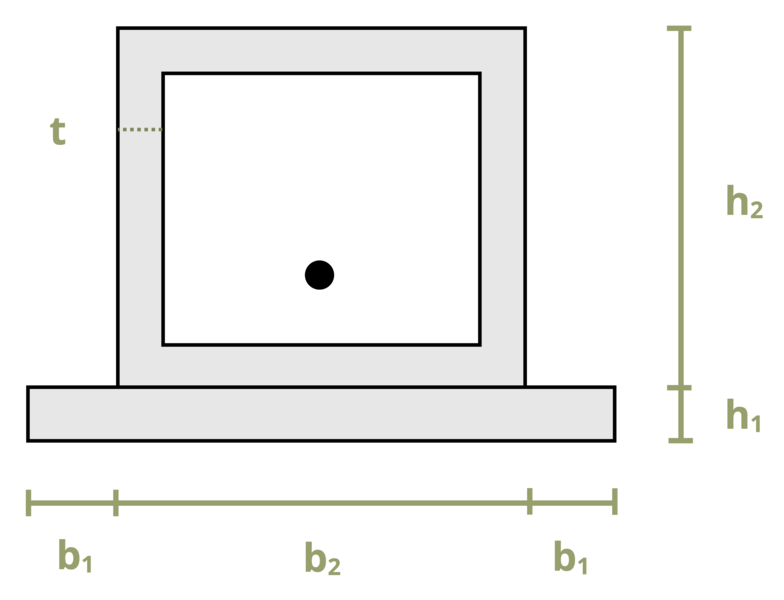
\includegraphics[keepaspectratio]{images/675.png}}
{[}Problem adapted from © Chris Galitz CC BY NC-SA 4.0{]}

\begin{Shaded}
\begin{Highlighting}[]
\NormalTok{\#| standalone: true}
\NormalTok{\#| viewerHeight: 600}
\NormalTok{\#| components: [viewer]}

\NormalTok{from shiny import App, render, ui, reactive}
\NormalTok{import random}
\NormalTok{import asyncio}
\NormalTok{import io}
\NormalTok{import math}
\NormalTok{import string}
\NormalTok{from datetime import datetime}
\NormalTok{from pathlib import Path}

\NormalTok{def generate\_random\_letters(length):}
\NormalTok{    \# Generate a random string of letters of specified length}
\NormalTok{    return \textquotesingle{}\textquotesingle{}.join(random.choice(string.ascii\_lowercase) for \_ in range(length))  }

\NormalTok{problem\_ID="675"}
\NormalTok{b1=reactive.Value("\_\_")}
\NormalTok{b2=reactive.Value("\_\_")}
\NormalTok{h1=reactive.Value("\_\_")}
\NormalTok{h2=reactive.Value("\_\_")}
\NormalTok{t=reactive.Value("\_\_")}
  
\NormalTok{attempts=["Timestamp,Attempt,Answer,Feedback\textbackslash{}n"]}

\NormalTok{app\_ui = ui.page\_fluid(}
\NormalTok{    \#ui.markdown("**Please enter your ID number from your instructor and click to generate your problem**"),}
\NormalTok{    \#ui.input\_text("ID","", placeholder="Enter ID Number Here"),}
\NormalTok{    \#ui.input\_action\_button("generate\_problem", "Generate Problem", class\_="btn{-}primary"),}
\NormalTok{    ui.markdown("**Problem Statement**"),}
\NormalTok{    ui.output\_ui("ui\_problem\_statement"),}
\NormalTok{    ui.input\_text("answer","Your Answer in units of mm", placeholder="Please enter your answer"),}
\NormalTok{    ui.input\_action\_button("submit", "Check Answer", class\_="btn{-}primary"),}
\NormalTok{    \#ui.download\_button("download", "Download File to Submit", class\_="btn{-}success"),}
\NormalTok{)}

\NormalTok{def server(input, output, session):}
\NormalTok{    \# Initialize a counter for attempts}
\NormalTok{    attempt\_counter = reactive.Value(0)}

\NormalTok{    @output}
\NormalTok{    @render.ui}
\NormalTok{    def ui\_problem\_statement():}
\NormalTok{        randomize\_vars()}
\NormalTok{        return[ui.markdown(f"For the composite cross{-}section shown, determine the centroid location, measured from the base. Assume dimensions b\textless{}sub\textgreater{}1\textless{}/sub\textgreater{} = \{b1()\} mm, b\textless{}sub\textgreater{}2\textless{}/sub\textgreater{} = \{b2()\} mm, h\textless{}sub\textgreater{}1\textless{}/sub\textgreater{} = \{h1()\} mm, h\textless{}sub\textgreater{}2\textless{}/sub\textgreater{} = \{h2()\} mm, and t = \{t()\} mm.")]}
    
\NormalTok{    \#@reactive.Effect}
\NormalTok{    \#@reactive.event(input.generate\_problem)}
\NormalTok{    def randomize\_vars():}
\NormalTok{        random.seed(101)}
\NormalTok{        b1.set(random.randrange(20,50,1))}
\NormalTok{        b2.set(round(b1(),1)*round(random.randrange(50,70,1)/10))}
\NormalTok{        h1.set(random.randrange(5,10,1))}
\NormalTok{        h2.set(b2())}
\NormalTok{        t.set(random.randrange(3,10,1))}
        
\NormalTok{    @reactive.Effect}
\NormalTok{    @reactive.event(input.submit)}
\NormalTok{    def \_():}
\NormalTok{        attempt\_counter.set(attempt\_counter() + 1)  \# Increment the attempt counter on each submission.}
\NormalTok{        y1 = h1()+h2()/2}
\NormalTok{        y2 = y1}
\NormalTok{        y3 = h1()/2}
\NormalTok{        A1 = h2()*b2()}
\NormalTok{        A2 = {-}(b2(){-}2*t())*(h2(){-}2*t())}
\NormalTok{        A3 = h1()*(2*b1()+b2())}
\NormalTok{        instr = (y1*A1+y2*A2+y3*A3)/(A1+A2+A3)}

\NormalTok{        if math.isclose(float(input.answer()), instr, rel\_tol=0.01):}
\NormalTok{            check = "*Correct*"}
\NormalTok{            correct\_indicator = "JL"}
\NormalTok{        else:}
\NormalTok{            check = "*Not Correct.*"}
\NormalTok{            correct\_indicator = "JG"}

\NormalTok{        \# Generate random parts for the encoded attempt.}
\NormalTok{        random\_start = generate\_random\_letters(4)}
\NormalTok{        random\_middle = generate\_random\_letters(4)}
\NormalTok{        random\_end = generate\_random\_letters(4)}
\NormalTok{        \#encoded\_attempt = f"\{random\_start\}\{problem\_ID\}{-}\{random\_middle\}\{attempt\_counter()\}\{correct\_indicator\}{-}\{random\_end\}\{input.ID()\}"}

\NormalTok{        \# Store the most recent encoded attempt in a reactive value so it persists across submissions}
\NormalTok{        \#session.encoded\_attempt = reactive.Value(encoded\_attempt)}

\NormalTok{        \# Append the attempt data to the attempts list without the encoded attempt}
\NormalTok{        attempts.append(f"\{datetime.now()\}, \{attempt\_counter()\}, \{input.answer()\}, \{check\}\textbackslash{}n")}

\NormalTok{        \# Show feedback to the user.}
\NormalTok{        feedback = ui.markdown(f"Your answer of \{input.answer()\} is \{check\}.")}
\NormalTok{        m = ui.modal(}
\NormalTok{            feedback,}
\NormalTok{            title="Feedback",}
\NormalTok{            easy\_close=True}
\NormalTok{        )}
\NormalTok{        ui.modal\_show(m)}

\NormalTok{    \#@render.download(filename=lambda: f"Problem\_Log{-}\{problem\_ID\}{-}\{input.ID()\}.csv")}
\NormalTok{    async def download():}
\NormalTok{        \# Start the CSV with the encoded attempt (without label)}
\NormalTok{        final\_encoded = session.encoded\_attempt() if session.encoded\_attempt is not None else "No attempts"}
\NormalTok{        yield f"\{final\_encoded\}\textbackslash{}n\textbackslash{}n"}
        
\NormalTok{        \# Write the header for the remaining CSV data once}
\NormalTok{        yield "Timestamp,Attempt,Answer,Feedback\textbackslash{}n"}
        
\NormalTok{        \# Write the attempts data, ensure that the header from the attempts list is not written again}
\NormalTok{        for attempt in attempts[1:]:  \# Skip the first element which is the header}
\NormalTok{            await asyncio.sleep(0.25)  \# This delay may not be necessary; adjust as needed}
\NormalTok{            yield attempt}

\NormalTok{\# App installation}
\NormalTok{app = App(app\_ui, server)}
\end{Highlighting}
\end{Shaded}

\chapter*{Problem 8.2 - Centroid}\label{problem-8.2---centroid}
\addcontentsline{toc}{chapter}{Problem 8.2 - Centroid}

\markboth{Problem 8.2 - Centroid}{Problem 8.2 - Centroid}

\pandocbounded{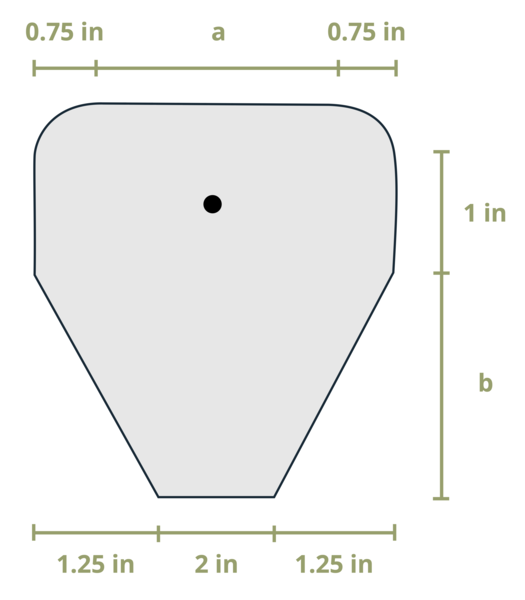
\includegraphics[keepaspectratio]{images/676.png}}
{[}Problem adapted from © Chris Galitz CC BY NC-SA 4.0{]}

\begin{Shaded}
\begin{Highlighting}[]
\NormalTok{\#| standalone: true}
\NormalTok{\#| viewerHeight: 600}
\NormalTok{\#| components: [viewer]}

\NormalTok{from shiny import App, render, ui, reactive}
\NormalTok{import random}
\NormalTok{import asyncio}
\NormalTok{import io}
\NormalTok{import math}
\NormalTok{import string}
\NormalTok{from datetime import datetime}
\NormalTok{from pathlib import Path}

\NormalTok{def generate\_random\_letters(length):}
\NormalTok{    \# Generate a random string of letters of specified length}
\NormalTok{    return \textquotesingle{}\textquotesingle{}.join(random.choice(string.ascii\_lowercase) for \_ in range(length))  }

\NormalTok{problem\_ID="676"}
\NormalTok{a=reactive.Value("\_\_")}
\NormalTok{b=reactive.Value("\_\_")}

\NormalTok{attempts=["Timestamp,Attempt,Answer,Feedback\textbackslash{}n"]}

\NormalTok{app\_ui = ui.page\_fluid(}
\NormalTok{    \#ui.markdown("**Please enter your ID number from your instructor and click to generate your problem**"),}
\NormalTok{    \#ui.input\_text("ID","", placeholder="Enter ID Number Here"),}
\NormalTok{    \#ui.input\_action\_button("generate\_problem", "Generate Problem", class\_="btn{-}primary"),}
\NormalTok{    ui.markdown("**Problem Statement**"),}
\NormalTok{    ui.output\_ui("ui\_problem\_statement"),}
\NormalTok{    ui.input\_text("answer","Your Answer in units of in", placeholder="Please enter your answer"),}
\NormalTok{    ui.input\_action\_button("submit", "Check Answer", class\_="btn{-}primary"),}
\NormalTok{    \#ui.download\_button("download", "Download File to Submit", class\_="btn{-}success"),}
\NormalTok{)}

\NormalTok{def server(input, output, session):}
\NormalTok{    \# Initialize a counter for attempts}
\NormalTok{    attempt\_counter = reactive.Value(0)}

\NormalTok{    @output}
\NormalTok{    @render.ui}
\NormalTok{    def ui\_problem\_statement():}
\NormalTok{        randomize\_vars()}
\NormalTok{        return[ui.markdown(f"For the beam cross{-}section shown, determine the centroid location, measured from the top surface. Assume dimensions a = 3 in. and b = \{b()\} in.")]}
    
\NormalTok{    \#@reactive.Effect}
\NormalTok{    \#@reactive.event(input.generate\_problem)}
\NormalTok{    def randomize\_vars():}
\NormalTok{        random.seed(101)}
\NormalTok{        b.set(random.randrange(30, 50, 1)/10)}
        
\NormalTok{    @reactive.Effect}
\NormalTok{    @reactive.event(input.submit)}
\NormalTok{    def \_():}
\NormalTok{        attempt\_counter.set(attempt\_counter() + 1)  \# Increment the attempt counter on each submission.}
\NormalTok{        y1 = 0.4317}
\NormalTok{        y2 = y1}
\NormalTok{        y3 = 0.375}
\NormalTok{        y4 = 1.25}
\NormalTok{        y5 = 1.75+b()/3}
\NormalTok{        y6 = y5}
\NormalTok{        y7 = 1.75+b()/2}
\NormalTok{        A1 = 0.4418}
\NormalTok{        A2 = A1}
\NormalTok{        A3 = 3*0.75}
\NormalTok{        A4 = 4.5}
\NormalTok{        A5 = 0.625*b()}
\NormalTok{        A6 = A5}
\NormalTok{        A7 = 2*b()}
\NormalTok{        instr= (y1*A1+y2*A2+y3*A3+y4*A4+y5*A5+y6*A6+y7*A7)/(A1+A2+A3+A4+A5+A6+A7)}
\NormalTok{        if math.isclose(float(input.answer()), instr, rel\_tol=0.01):}
\NormalTok{            check = "*Correct*"}
\NormalTok{            correct\_indicator = "JL"}
\NormalTok{        else:}
\NormalTok{            check = "*Not Correct.*"}
\NormalTok{            correct\_indicator = "JG"}

\NormalTok{        \# Generate random parts for the encoded attempt.}
\NormalTok{        random\_start = generate\_random\_letters(4)}
\NormalTok{        random\_middle = generate\_random\_letters(4)}
\NormalTok{        random\_end = generate\_random\_letters(4)}
\NormalTok{        \#encoded\_attempt = f"\{random\_start\}\{problem\_ID\}{-}\{random\_middle\}\{attempt\_counter()\}\{correct\_indicator\}{-}\{random\_end\}\{input.ID()\}"}

\NormalTok{        \# Store the most recent encoded attempt in a reactive value so it persists across submissions}
\NormalTok{        \#session.encoded\_attempt = reactive.Value(encoded\_attempt)}

\NormalTok{        \# Append the attempt data to the attempts list without the encoded attempt}
\NormalTok{        attempts.append(f"\{datetime.now()\}, \{attempt\_counter()\}, \{input.answer()\}, \{check\}\textbackslash{}n")}

\NormalTok{        \# Show feedback to the user.}
\NormalTok{        feedback = ui.markdown(f"Your answer of \{input.answer()\} is \{check\}.")}
\NormalTok{        m = ui.modal(}
\NormalTok{            feedback,}
\NormalTok{            title="Feedback",}
\NormalTok{            easy\_close=True}
\NormalTok{        )}
\NormalTok{        ui.modal\_show(m)}

\NormalTok{    \#@render.download(filename=lambda: f"Problem\_Log{-}\{problem\_ID\}{-}\{input.ID()\}.csv")}
\NormalTok{    async def download():}
\NormalTok{        \# Start the CSV with the encoded attempt (without label)}
\NormalTok{        final\_encoded = session.encoded\_attempt() if session.encoded\_attempt is not None else "No attempts"}
\NormalTok{        yield f"\{final\_encoded\}\textbackslash{}n\textbackslash{}n"}
        
\NormalTok{        \# Write the header for the remaining CSV data once}
\NormalTok{        yield "Timestamp,Attempt,Answer,Feedback\textbackslash{}n"}
        
\NormalTok{        \# Write the attempts data, ensure that the header from the attempts list is not written again}
\NormalTok{        for attempt in attempts[1:]:  \# Skip the first element which is the header}
\NormalTok{            await asyncio.sleep(0.25)  \# This delay may not be necessary; adjust as needed}
\NormalTok{            yield attempt}

\NormalTok{\# App installation}
\NormalTok{app = App(app\_ui, server)}
\end{Highlighting}
\end{Shaded}

\chapter*{Problem 8.3 - Centroid}\label{problem-8.3---centroid}
\addcontentsline{toc}{chapter}{Problem 8.3 - Centroid}

\markboth{Problem 8.3 - Centroid}{Problem 8.3 - Centroid}

\pandocbounded{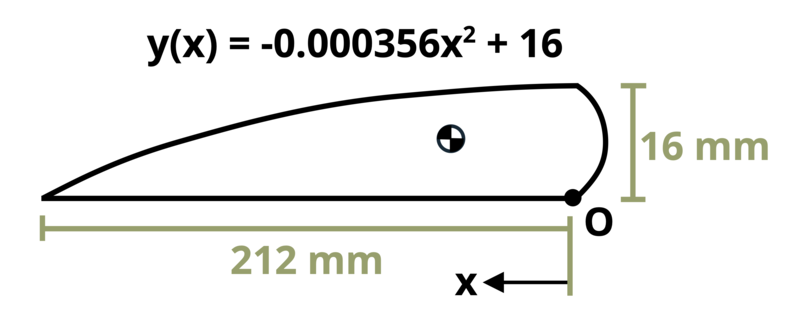
\includegraphics[keepaspectratio]{images/677.png}}
{[}Problem adapted from © Chris Galitz CC BY NC-SA 4.0{]}

\begin{Shaded}
\begin{Highlighting}[]
\NormalTok{\#| standalone: true}
\NormalTok{\#| viewerHeight: 600}
\NormalTok{\#| components: [viewer]}

\NormalTok{from shiny import App, render, ui, reactive}
\NormalTok{import random}
\NormalTok{import asyncio}
\NormalTok{import io}
\NormalTok{import math}
\NormalTok{import string}
\NormalTok{from datetime import datetime}
\NormalTok{from pathlib import Path}

\NormalTok{def generate\_random\_letters(length):}
\NormalTok{    \# Generate a random string of letters of specified length}
\NormalTok{    return "".join(random.choice(string.ascii\_lowercase) for \_ in range(length))}

\NormalTok{problem\_ID = "677"}
\NormalTok{a = reactive.Value("\_\_")}
\NormalTok{b = reactive.Value("\_\_")}
\NormalTok{attempts = ["Timestamp,Attempt,Answer1,Answer2,Feedback\textbackslash{}n"]}

\NormalTok{app\_ui = ui.page\_fluid(}
\NormalTok{    \#ui.markdown("**Please enter your ID number from your instructor and click to generate your problem**"),}
\NormalTok{    \#ui.input\_text("ID", "", placeholder="Enter ID Number Here"),}
\NormalTok{    \#ui.input\_action\_button("generate\_problem", "Generate Problem", class\_="btn{-}primary"),}
\NormalTok{    ui.markdown("**Problem Statement**"),}
\NormalTok{    ui.output\_ui("ui\_problem\_statement"),}
\NormalTok{    ui.input\_text("answer1", "Your Answer 1 in units of mm", placeholder="Please enter your answer 1"),}
\NormalTok{    ui.input\_text("answer2", "Your Answer 2 in units of mm", placeholder="Please enter your answer 2"),}
\NormalTok{    ui.input\_action\_button("submit", "Check Answers", class\_="btn{-}primary"),}
\NormalTok{    \#ui.download\_button("download", "Download File to Submit", class\_="btn{-}success"),}
\NormalTok{)}

\NormalTok{def server(input, output, session):}
\NormalTok{    \# Initialize a counter for attempts}
\NormalTok{    attempt\_counter = reactive.Value(0)}

\NormalTok{    @output}
\NormalTok{    @render.ui}
\NormalTok{    def ui\_problem\_statement():}
\NormalTok{        randomize\_vars()}
\NormalTok{        return [}
\NormalTok{            ui.markdown(}
\NormalTok{                f"An experimental model aircraft wing incorporates a half{-}circular leading edge and a parabolic top surface. Determine the x{-} and y{-}coordinates of the centroid of the cross{-}section. Assume dimensions a = \{a()\} mm and b = \{b()\} mm."}
\NormalTok{            )}
\NormalTok{        ]}

\NormalTok{    \#@reactive.Effect}
\NormalTok{    \#@reactive.event(input.generate\_problem)}
\NormalTok{    def randomize\_vars():}
\NormalTok{        random.seed(101)}
\NormalTok{        a.set(random.randrange(150,300,5))}
\NormalTok{        b.set(random.randrange(10,30,1))}
        
\NormalTok{    @reactive.Effect}
\NormalTok{    @reactive.event(input.submit)}
\NormalTok{    def \_():}
\NormalTok{        attempt\_counter.set(}
\NormalTok{            attempt\_counter() + 1}
\NormalTok{        )  \# Increment the attempt counter on each submission.}

\NormalTok{        \# Calculate the instructor\textquotesingle{}s answer and determine if the user\textquotesingle{}s answer is correct.}
\NormalTok{        xbar={-}0.000089*a()**4+b()/2*a()**2/({-}0.0001187*a()**3+b()*a())}
\NormalTok{        ybar=2.535*10**{-}8*a()**5{-}0.000356*b()*2/3*a()**3+b()**2*a()/({-}0.0001187*a()**3+b()*a())}
\NormalTok{        A1={-}0.0001187*a()**3+b()*a()}
\NormalTok{        A2=math.pi*b()**2/4}
\NormalTok{        x2={-}4*b()/2/(3*math.pi)}
\NormalTok{        x1A1=xbar*A1}
\NormalTok{        x2A2=x2*A2}
\NormalTok{        instr1=(x1A1+x2A2)/(A1+A2)}
\NormalTok{        y2=b()/2}
\NormalTok{        y1A1=ybar*A1}
\NormalTok{        y2A2=y2*A2}
\NormalTok{        instr2=(y1A1+y2A2)/(A1+A2)}

\NormalTok{        correct1 = math.isclose(float(input.answer1()), instr1, rel\_tol=0.01)}
\NormalTok{        correct2 = math.isclose(float(input.answer2()), instr2, rel\_tol=0.01)}
        
\NormalTok{        if correct1 and correct2:}
\NormalTok{            check = f"\{\textquotesingle{}both correct.\textquotesingle{}\}"}
\NormalTok{        elif correct1:}
\NormalTok{            check = f" \{\textquotesingle{}correct for answer 1 and incorrect for answer 2.\textquotesingle{}\}"}
\NormalTok{        elif correct2:}
\NormalTok{            check = f"\{\textquotesingle{}incorrect for answer 1 and correct for answer 2.\textquotesingle{}\}"}
\NormalTok{        else:}
\NormalTok{            check = f"\{\textquotesingle{}both incorrect.\textquotesingle{}\}"}
        
\NormalTok{        correct\_indicator = "JL" if correct1 and correct2 else "JG"}

\NormalTok{        random\_start = generate\_random\_letters(4)}
\NormalTok{        random\_middle = generate\_random\_letters(4)}
\NormalTok{        random\_end = generate\_random\_letters(4)}
\NormalTok{        \#encoded\_attempt = f"\{random\_start\}\{problem\_ID\}{-}\{random\_middle\}\{attempt\_counter()\}\{correct\_indicator\}{-}\{random\_end\}\{input.ID()\}"}

\NormalTok{        \#session.encoded\_attempt = reactive.Value(encoded\_attempt)}
\NormalTok{        attempts.append(f"\{datetime.now()\}, \{attempt\_counter()\}, \{input.answer1()\}, \{input.answer2()\}, \{check\}\textbackslash{}n")}

\NormalTok{        feedback = ui.markdown(f"Your answers of \{input.answer1()\} and \{input.answer2()\} are \{check\}")}
\NormalTok{        m = ui.modal(feedback, title="Feedback", easy\_close=True)}
\NormalTok{        ui.modal\_show(m)}

\NormalTok{    \#@render.download(filename=lambda: f"Problem\_Log{-}\{problem\_ID\}{-}\{input.ID()\}.csv")}
\NormalTok{    async def download():}
\NormalTok{        final\_encoded = session.encoded\_attempt() if session.encoded\_attempt is not None else "No attempts"}
\NormalTok{        yield f"\{final\_encoded\}\textbackslash{}n\textbackslash{}n"}
\NormalTok{        yield "Timestamp,Attempt,Answer1,Answer2,Feedback\textbackslash{}n"}
\NormalTok{        for attempt in attempts[1:]:}
\NormalTok{            await asyncio.sleep(0.25)}
\NormalTok{            yield attempt}

\NormalTok{app = App(app\_ui, server)}
\end{Highlighting}
\end{Shaded}

\chapter*{Problem 8.4 - Centroid}\label{problem-8.4---centroid}
\addcontentsline{toc}{chapter}{Problem 8.4 - Centroid}

\markboth{Problem 8.4 - Centroid}{Problem 8.4 - Centroid}

\pandocbounded{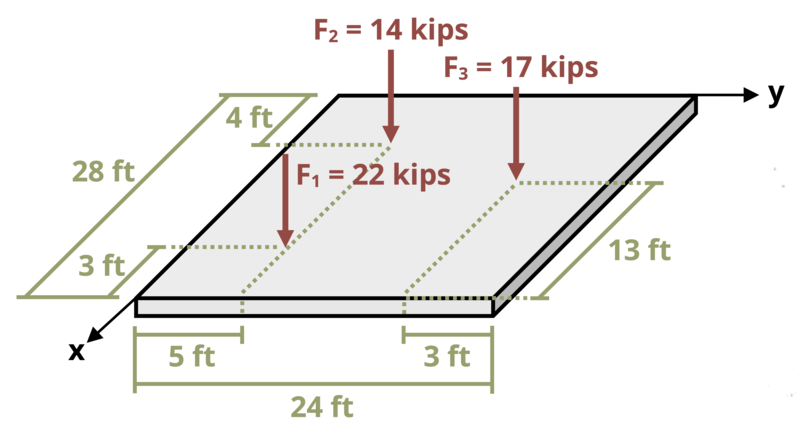
\includegraphics[keepaspectratio]{images/678.png}}
{[}Problem adapted from © Chris Galitz CC BY NC-SA 4.0{]}

\begin{Shaded}
\begin{Highlighting}[]
\NormalTok{\#| standalone: true}
\NormalTok{\#| viewerHeight: 600}
\NormalTok{\#| components: [viewer]}

\NormalTok{from shiny import App, render, ui, reactive}
\NormalTok{import random}
\NormalTok{import asyncio}
\NormalTok{import io}
\NormalTok{import math}
\NormalTok{import string}
\NormalTok{from datetime import datetime}
\NormalTok{from pathlib import Path}

\NormalTok{def generate\_random\_letters(length):}
\NormalTok{    \# Generate a random string of letters of specified length}
\NormalTok{    return "".join(random.choice(string.ascii\_lowercase) for \_ in range(length))}

\NormalTok{problem\_ID = "678"}
\NormalTok{w = reactive.Value("\_\_")}
\NormalTok{F1 = reactive.Value("\_\_")}
\NormalTok{F2 = reactive.Value("\_\_")}
\NormalTok{F3 = reactive.Value("\_\_")}
\NormalTok{attempts = ["Timestamp,Attempt,Answer1,Answer2,Feedback\textbackslash{}n"]}

\NormalTok{app\_ui = ui.page\_fluid(}
\NormalTok{    \#ui.markdown("**Please enter your ID number from your instructor and click to generate your problem**"),}
\NormalTok{    \#ui.input\_text("ID", "", placeholder="Enter ID Number Here"),}
\NormalTok{    \#ui.input\_action\_button("generate\_problem", "Generate Problem", class\_="btn{-}primary"),}
\NormalTok{    ui.markdown("**Problem Statement**"),}
\NormalTok{    ui.output\_ui("ui\_problem\_statement"),}
\NormalTok{    ui.input\_text("answer1", "Your Answer 1 in units of ft", placeholder="Please enter your answer 1"),}
\NormalTok{    ui.input\_text("answer2", "Your Answer 2 in units of ft", placeholder="Please enter your answer 2"),}
\NormalTok{    ui.input\_action\_button("submit", "Check Answers", class\_="btn{-}primary"),}
\NormalTok{    \#ui.download\_button("download", "Download File to Submit", class\_="btn{-}success"),}
\NormalTok{)}

\NormalTok{def server(input, output, session):}
\NormalTok{    \# Initialize a counter for attempts}
\NormalTok{    attempt\_counter = reactive.Value(0)}

\NormalTok{    @output}
\NormalTok{    @render.ui}
\NormalTok{    def ui\_problem\_statement():}
\NormalTok{        randomize\_vars()}
\NormalTok{        return [}
\NormalTok{            ui.markdown(}
\NormalTok{                f"A parking garage slab is subject to an area load ω = \{w()\} lb/ft\textless{}sup\textgreater{}2\textless{}/sup\textgreater{} and point loads F\textless{}sub\textgreater{}1\textless{}/sub\textgreater{} = \{F1()\} kips, F\textless{}sub\textgreater{}2\textless{}/sub\textgreater{} = \{F2()\} kips, and F\textless{}sub\textgreater{}3\textless{}/sub\textgreater{} = \{F3()\} kips. Determine the x{-} and y{-}coordinates of the denter of the loading."}
\NormalTok{            )}
\NormalTok{        ]}

\NormalTok{    \#@reactive.Effect}
\NormalTok{    \#@reactive.event(input.generate\_problem)}
\NormalTok{    def randomize\_vars():}
\NormalTok{        random.seed(101)}
\NormalTok{        w.set(random.randrange(20,50,1))}
\NormalTok{        F1.set(random.randrange(10,30,1))}
\NormalTok{        F2.set(random.randrange(10,30,1))}
\NormalTok{        F3.set(random.randrange(10,30,1))}
        
\NormalTok{    @reactive.Effect}
\NormalTok{    @reactive.event(input.submit)}
\NormalTok{    def \_():}
\NormalTok{        attempt\_counter.set(}
\NormalTok{            attempt\_counter() + 1}
\NormalTok{        )  \# Increment the attempt counter on each submission.}

\NormalTok{        \# Calculate the instructor\textquotesingle{}s answer and determine if the user\textquotesingle{}s answer is correct.}
\NormalTok{        Fog=w()*28*24/1000}
\NormalTok{        F1xF=F1()*25}
\NormalTok{        F2xF=F2()*4}
\NormalTok{        F3xF=F3()*15}
\NormalTok{        FogxF=Fog*14}
\NormalTok{        instr1 = (F1xF+F2xF+F2xF+FogxF)/(F1()+F2()+F3()+Fog)}
\NormalTok{        F1yF=F1()*5}
\NormalTok{        F2yF=F2()*5}
\NormalTok{        F3yF=F3()*21}
\NormalTok{        FogyF=Fog*12}
\NormalTok{        instr2 = (F1yF+F2yF+F3yF+FogyF)/(F1()+F2()+F3()+Fog)}

\NormalTok{        correct1 = math.isclose(float(input.answer1()), instr1, rel\_tol=0.01)}
\NormalTok{        correct2 = math.isclose(float(input.answer2()), instr2, rel\_tol=0.01)}
        
\NormalTok{        if correct1 and correct2:}
\NormalTok{            check = f"\{\textquotesingle{}both correct.\textquotesingle{}\}"}
\NormalTok{        elif correct1:}
\NormalTok{            check = f" \{\textquotesingle{}correct for answer 1 and incorrect for answer 2.\textquotesingle{}\}"}
\NormalTok{        elif correct2:}
\NormalTok{            check = f"\{\textquotesingle{}incorrect for answer 1 and correct for answer 2.\textquotesingle{}\}"}
\NormalTok{        else:}
\NormalTok{            check = f"\{\textquotesingle{}both incorrect.\textquotesingle{}\}"}
        
\NormalTok{        correct\_indicator = "JL" if correct1 and correct2 else "JG"}

\NormalTok{        random\_start = generate\_random\_letters(4)}
\NormalTok{        random\_middle = generate\_random\_letters(4)}
\NormalTok{        random\_end = generate\_random\_letters(4)}
\NormalTok{        \#encoded\_attempt = f"\{random\_start\}\{problem\_ID\}{-}\{random\_middle\}\{attempt\_counter()\}\{correct\_indicator\}{-}\{random\_end\}\{input.ID()\}"}

\NormalTok{        \#session.encoded\_attempt = reactive.Value(encoded\_attempt)}
\NormalTok{        attempts.append(f"\{datetime.now()\}, \{attempt\_counter()\}, \{input.answer1()\}, \{input.answer2()\}, \{check\}\textbackslash{}n")}

\NormalTok{        feedback = ui.markdown(f"Your answers of \{input.answer1()\} and \{input.answer2()\} are \{check\}.")}
\NormalTok{        m = ui.modal(feedback, title="Feedback", easy\_close=True)}
\NormalTok{        ui.modal\_show(m)}

\NormalTok{    \#@render.download(filename=lambda: f"Problem\_Log{-}\{problem\_ID\}{-}\{input.ID()\}.csv")}
\NormalTok{    async def download():}
\NormalTok{        final\_encoded = session.encoded\_attempt() if session.encoded\_attempt is not None else "No attempts"}
\NormalTok{        yield f"\{final\_encoded\}\textbackslash{}n\textbackslash{}n"}
\NormalTok{        yield "Timestamp,Attempt,Answer1,Answer2,Feedback\textbackslash{}n"}
\NormalTok{        for attempt in attempts[1:]:}
\NormalTok{            await asyncio.sleep(0.25)}
\NormalTok{            yield attempt}

\NormalTok{app = App(app\_ui, server)}
\end{Highlighting}
\end{Shaded}

\chapter*{Problem 8.5 - Centroid}\label{problem-8.5---centroid}
\addcontentsline{toc}{chapter}{Problem 8.5 - Centroid}

\markboth{Problem 8.5 - Centroid}{Problem 8.5 - Centroid}

\pandocbounded{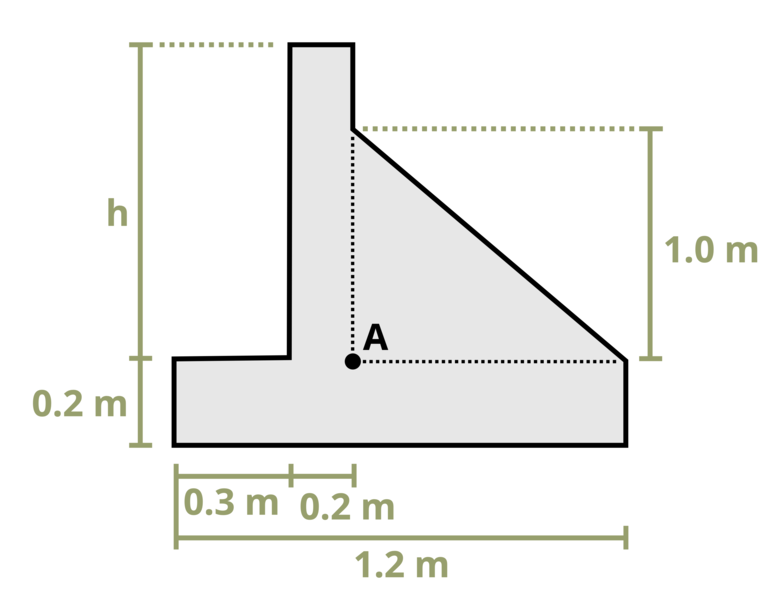
\includegraphics[keepaspectratio]{images/679.png}}
{[}Problem adapted from © Chris Galitz CC BY NC-SA 4.0{]}

\begin{Shaded}
\begin{Highlighting}[]
\NormalTok{\#| standalone: true}
\NormalTok{\#| viewerHeight: 600}
\NormalTok{\#| components: [viewer]}

\NormalTok{from shiny import App, render, ui, reactive}
\NormalTok{import random}
\NormalTok{import asyncio}
\NormalTok{import io}
\NormalTok{import math}
\NormalTok{import string}
\NormalTok{from datetime import datetime}
\NormalTok{from pathlib import Path}

\NormalTok{def generate\_random\_letters(length):}
\NormalTok{    \# Generate a random string of letters of specified length}
\NormalTok{    return \textquotesingle{}\textquotesingle{}.join(random.choice(string.ascii\_lowercase) for \_ in range(length))  }

\NormalTok{problem\_ID="679"}
\NormalTok{a=reactive.Value("\_\_")}
\NormalTok{b=reactive.Value("\_\_")}
  
\NormalTok{attempts=["Timestamp,Attempt,Answer,Feedback\textbackslash{}n"]}

\NormalTok{app\_ui = ui.page\_fluid(}
\NormalTok{    \#ui.markdown("**Please enter your ID number from your instructor and click to generate your problem**"),}
\NormalTok{    \#ui.input\_text("ID","", placeholder="Enter ID Number Here"),}
\NormalTok{    \#ui.input\_action\_button("generate\_problem", "Generate Problem", class\_="btn{-}primary"),}
\NormalTok{    ui.markdown("**Problem Statement**"),}
\NormalTok{    ui.output\_ui("ui\_problem\_statement"),}
\NormalTok{    ui.input\_text("answer","Your Answer in units of m", placeholder="Please enter your answer"),}
\NormalTok{    ui.input\_action\_button("submit", "Check Answer", class\_="btn{-}primary"),}
\NormalTok{    \#ui.download\_button("download", "Download File to Submit", class\_="btn{-}success"),}
\NormalTok{)}


\NormalTok{def server(input, output, session):}
\NormalTok{    \# Initialize a counter for attempts}
\NormalTok{    attempt\_counter = reactive.Value(0)}

\NormalTok{    @output}
\NormalTok{    @render.ui}
\NormalTok{    def ui\_problem\_statement():}
\NormalTok{        randomize\_vars()}
\NormalTok{        return[ui.markdown(f"The cross{-}section shown is to be used as a retaining structure. Determine the tallest height, h, such that the shape\textquotesingle{}s centroid is to the right of point A. Assume dimensions a = \{a()\} m and b = \{b()\} m.")]}
    
\NormalTok{    \#@reactive.Effect}
\NormalTok{    \#@reactive.event(input.generate\_problem)}
\NormalTok{    def randomize\_vars():}
\NormalTok{        random.seed(101)}
\NormalTok{        a.set(random.randrange(10,30,1)/10)}
\NormalTok{        b.set(random.randrange(10,30,1)/10)}
        
\NormalTok{    @reactive.Effect}
\NormalTok{    @reactive.event(input.submit)}
\NormalTok{    def \_():}
\NormalTok{        attempt\_counter.set(attempt\_counter() + 1)  \# Increment the attempt counter on each submission.}
\NormalTok{        VertxA=0.02}
\NormalTok{        HorxA=(a()/2{-}0.5)*a()*0.2}
\NormalTok{        TrixA=(a(){-}0.5)/3*0.5*(a(){-}0.5)*b()}
\NormalTok{        instr= (HorxA+TrixA)/VertxA}
\NormalTok{        if math.isclose(float(input.answer()), instr, rel\_tol=0.01):}
\NormalTok{            check = "*Correct*"}
\NormalTok{            correct\_indicator = "JL"}
\NormalTok{        else:}
\NormalTok{            check = "*Not Correct.*"}
\NormalTok{            correct\_indicator = "JG"}

\NormalTok{        \# Generate random parts for the encoded attempt.}
\NormalTok{        random\_start = generate\_random\_letters(4)}
\NormalTok{        random\_middle = generate\_random\_letters(4)}
\NormalTok{        random\_end = generate\_random\_letters(4)}
\NormalTok{        \#encoded\_attempt = f"\{random\_start\}\{problem\_ID\}{-}\{random\_middle\}\{attempt\_counter()\}\{correct\_indicator\}{-}\{random\_end\}\{input.ID()\}"}

\NormalTok{        \# Store the most recent encoded attempt in a reactive value so it persists across submissions}
\NormalTok{        \#session.encoded\_attempt = reactive.Value(encoded\_attempt)}

\NormalTok{        \# Append the attempt data to the attempts list without the encoded attempt}
\NormalTok{        attempts.append(f"\{datetime.now()\}, \{attempt\_counter()\}, \{input.answer()\}, \{check\}\textbackslash{}n")}

\NormalTok{        \# Show feedback to the user.}
\NormalTok{        feedback = ui.markdown(f"Your answer of \{input.answer()\} is \{check\}.")}
\NormalTok{        m = ui.modal(}
\NormalTok{            feedback,}
\NormalTok{            title="Feedback",}
\NormalTok{            easy\_close=True}
\NormalTok{        )}
\NormalTok{        ui.modal\_show(m)}

\NormalTok{    \#@render.download(filename=lambda: f"Problem\_Log{-}\{problem\_ID\}{-}\{input.ID()\}.csv")}
\NormalTok{    async def download():}
\NormalTok{        \# Start the CSV with the encoded attempt (without label)}
\NormalTok{        final\_encoded = session.encoded\_attempt() if session.encoded\_attempt is not None else "No attempts"}
\NormalTok{        yield f"\{final\_encoded\}\textbackslash{}n\textbackslash{}n"}
        
\NormalTok{        \# Write the header for the remaining CSV data once}
\NormalTok{        yield "Timestamp,Attempt,Answer,Feedback\textbackslash{}n"}
        
\NormalTok{        \# Write the attempts data, ensure that the header from the attempts list is not written again}
\NormalTok{        for attempt in attempts[1:]:  \# Skip the first element which is the header}
\NormalTok{            await asyncio.sleep(0.25)  \# This delay may not be necessary; adjust as needed}
\NormalTok{            yield attempt}

\NormalTok{\# App installation}
\NormalTok{app = App(app\_ui, server)}
\end{Highlighting}
\end{Shaded}

\chapter*{Problem 8.7 - Area Moment of
Inertia}\label{problem-8.7---area-moment-of-inertia}
\addcontentsline{toc}{chapter}{Problem 8.7 - Area Moment of Inertia}

\markboth{Problem 8.7 - Area Moment of Inertia}{Problem 8.7 - Area
Moment of Inertia}

\pandocbounded{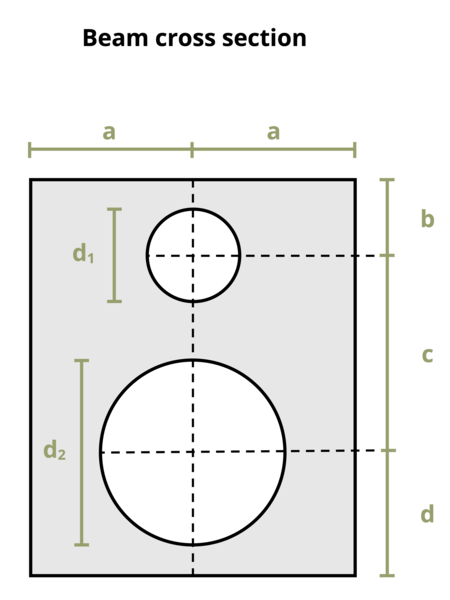
\includegraphics[keepaspectratio]{images/347.png}}
{[}Problem adapted from © Kurt Gramoll CC BY NC-SA 4.0{]}

\begin{Shaded}
\begin{Highlighting}[]
\NormalTok{\#| standalone: true}
\NormalTok{\#| viewerHeight: 600}
\NormalTok{\#| components: [viewer]}

\NormalTok{from shiny import App, render, ui, reactive}
\NormalTok{import random}
\NormalTok{import asyncio}
\NormalTok{import io}
\NormalTok{import math}
\NormalTok{import string}
\NormalTok{from datetime import datetime}
\NormalTok{from pathlib import Path}

\NormalTok{def generate\_random\_letters(length):}
\NormalTok{    \# Generate a random string of letters of specified length}
\NormalTok{    return \textquotesingle{}\textquotesingle{}.join(random.choice(string.ascii\_lowercase) for \_ in range(length))  }

\NormalTok{problem\_ID="347"}
\NormalTok{b=reactive.Value("\_\_")}
\NormalTok{c=reactive.Value("\_\_")}
\NormalTok{d=reactive.Value("\_\_")}
\NormalTok{a=reactive.Value("\_\_")}
\NormalTok{d1=reactive.Value("\_\_")}
\NormalTok{d2=reactive.Value("\_\_")}
  
\NormalTok{attempts=["Timestamp,Attempt,Answer,Feedback\textbackslash{}n"]}

\NormalTok{app\_ui = ui.page\_fluid(}
\NormalTok{    \#ui.markdown("**Please enter your ID number from your instructor and click to generate your problem**"),}
\NormalTok{    \#ui.input\_text("ID","", placeholder="Enter ID Number Here"),}
\NormalTok{    \#ui.input\_action\_button("generate\_problem", "Generate Problem", class\_="btn{-}primary"),}
\NormalTok{    ui.markdown("**Problem Statement**"),}
\NormalTok{    ui.output\_ui("ui\_problem\_statement"),}
\NormalTok{    ui.input\_text("answer","Your Answer in units of in\textbackslash{}u2074", placeholder="Please enter your answer"),}
\NormalTok{    ui.input\_action\_button("submit", "Check Answer", class\_="btn{-}primary"),}
\NormalTok{    \#ui.download\_button("download", "Download File to Submit", class\_="btn{-}success"),}
\NormalTok{)}

\NormalTok{def server(input, output, session):}
\NormalTok{    \# Initialize a counter for attempts}
\NormalTok{    attempt\_counter = reactive.Value(0)}

\NormalTok{    @output}
\NormalTok{    @render.ui}
\NormalTok{    def ui\_problem\_statement():}
\NormalTok{        randomize\_vars()}
\NormalTok{        return[ui.markdown(f"The cross{-}section shows a concrete beam with two hollow round holes. Determine the area moment of inertia about the beam\textquotesingle{}s centroid. Assume lengths a = \{a()\} in., b = \{b()\} in., c = \{c()\} in., d = \{d()\} in., d\textless{}sub\textgreater{}1\textless{}/sub\textgreater{} = \{d1()\} in., and d\textless{}sub\textgreater{}2\textless{}/sub\textgreater{} = \{d2()\} in.")]}
    
\NormalTok{    \#@reactive.Effect}
\NormalTok{    \#@reactive.event(input.generate\_problem)}
\NormalTok{    def randomize\_vars():}
\NormalTok{        random.seed(101)}
\NormalTok{        b.set(random.randrange(20, 60, 1)/10)}
\NormalTok{        c.set(round(b()*3,1))}
\NormalTok{        d.set(b()*2)}
\NormalTok{        a.set(b()*2.5)}
\NormalTok{        d1.set(round(b()*1.5,1))}
\NormalTok{        d2.set(d1()*2)}
        
\NormalTok{    @reactive.Effect}
\NormalTok{    @reactive.event(input.submit)}
\NormalTok{    def \_():}
\NormalTok{        attempt\_counter.set(attempt\_counter() + 1)  \# Increment the attempt counter on each submission.}
\NormalTok{        A1 = (b()+c()+d())*2*a()}
\NormalTok{        h1 = (b()+c()+d())/2}
\NormalTok{        A2 = (d2()/2)**2*math.pi}
\NormalTok{        h2 = d()}
\NormalTok{        A3 = (d1()/2)**2*math.pi}
\NormalTok{        h3 = d()+c()}
\NormalTok{        h = (A1*h1{-}A2*h2{-}A3*h3)/(A1{-}A2{-}A3)}
\NormalTok{        y1 = h{-}h1}
\NormalTok{        y2 = h{-}h2}
\NormalTok{        y3 = h{-}h3}
\NormalTok{        I1 = 2*a()*(b()+c()+d())**3/12}
\NormalTok{        I2 = (d2()/2)**4*math.pi/4}
\NormalTok{        I3 = (d1()/2)**4*math.pi/4}
\NormalTok{        instr = I1+A1*y1**2{-}(I2+A2*y2**2){-}(I3+A3*y3**2)}

\NormalTok{        if math.isclose(float(input.answer()), instr, rel\_tol=0.01):}
\NormalTok{            check = "*Correct*"}
\NormalTok{            correct\_indicator = "JL"}
\NormalTok{        else:}
\NormalTok{            check = "*Not Correct.*"}
\NormalTok{            correct\_indicator = "JG"}

\NormalTok{        \# Generate random parts for the encoded attempt.}
\NormalTok{        random\_start = generate\_random\_letters(4)}
\NormalTok{        random\_middle = generate\_random\_letters(4)}
\NormalTok{        random\_end = generate\_random\_letters(4)}
\NormalTok{        \#encoded\_attempt = f"\{random\_start\}\{problem\_ID\}{-}\{random\_middle\}\{attempt\_counter()\}\{correct\_indicator\}{-}\{random\_end\}\{input.ID()\}"}

\NormalTok{        \# Store the most recent encoded attempt in a reactive value so it persists across submissions}
\NormalTok{        \#session.encoded\_attempt = reactive.Value(encoded\_attempt)}

\NormalTok{        \# Append the attempt data to the attempts list without the encoded attempt}
\NormalTok{        attempts.append(f"\{datetime.now()\}, \{attempt\_counter()\}, \{input.answer()\}, \{check\}\textbackslash{}n")}

\NormalTok{        \# Show feedback to the user.}
\NormalTok{        feedback = ui.markdown(f"Your answer of \{input.answer()\} is \{check\}.")}
\NormalTok{        m = ui.modal(}
\NormalTok{            feedback,}
\NormalTok{            title="Feedback",}
\NormalTok{            easy\_close=True}
\NormalTok{        )}
\NormalTok{        ui.modal\_show(m)}

\NormalTok{    \#@render.download(filename=lambda: f"Problem\_Log{-}\{problem\_ID\}{-}\{input.ID()\}.csv")}
\NormalTok{    async def download():}
\NormalTok{        \# Start the CSV with the encoded attempt (without label)}
\NormalTok{        final\_encoded = session.encoded\_attempt() if session.encoded\_attempt is not None else "No attempts"}
\NormalTok{        yield f"\{final\_encoded\}\textbackslash{}n\textbackslash{}n"}
        
\NormalTok{        \# Write the header for the remaining CSV data once}
\NormalTok{        yield "Timestamp,Attempt,Answer,Feedback\textbackslash{}n"}
        
\NormalTok{        \# Write the attempts data, ensure that the header from the attempts list is not written again}
\NormalTok{        for attempt in attempts[1:]:  \# Skip the first element which is the header}
\NormalTok{            await asyncio.sleep(0.25)  \# This delay may not be necessary; adjust as needed}
\NormalTok{            yield attempt}

\NormalTok{\# App installation}
\NormalTok{app = App(app\_ui, server)}
\end{Highlighting}
\end{Shaded}

\part{Chapter 9 Problems}

\chapter*{Problem 9.1 - Bending
Stress}\label{problem-9.1---bending-stress}
\addcontentsline{toc}{chapter}{Problem 9.1 - Bending Stress}

\markboth{Problem 9.1 - Bending Stress}{Problem 9.1 - Bending Stress}

\pandocbounded{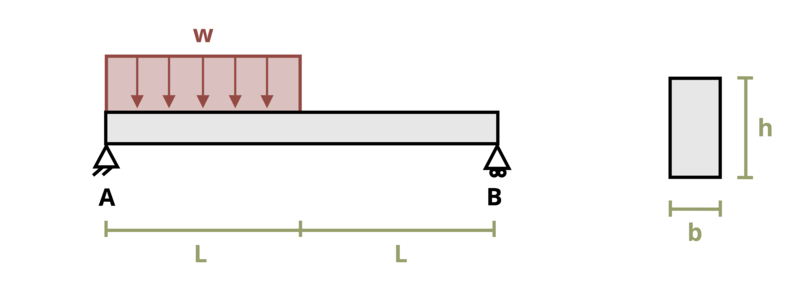
\includegraphics[keepaspectratio]{images/342.png}}
{[}Problem adapted from © Kurt Gramoll CC BY NC-SA 4.0{]}

\begin{Shaded}
\begin{Highlighting}[]
\NormalTok{\#| standalone: true}
\NormalTok{\#| viewerHeight: 600}
\NormalTok{\#| components: [viewer]}

\NormalTok{from shiny import App, render, ui, reactive}
\NormalTok{import random}
\NormalTok{import asyncio}
\NormalTok{import io}
\NormalTok{import math}
\NormalTok{import string}
\NormalTok{from datetime import datetime}
\NormalTok{from pathlib import Path}

\NormalTok{def generate\_random\_letters(length):}
\NormalTok{    \# Generate a random string of letters of specified length}
\NormalTok{    return \textquotesingle{}\textquotesingle{}.join(random.choice(string.ascii\_lowercase) for \_ in range(length))  }

\NormalTok{problem\_ID="342"}
\NormalTok{b=reactive.Value("\_\_")}
\NormalTok{h=reactive.Value("\_\_")}
\NormalTok{w=reactive.Value("\_\_")}
\NormalTok{L=reactive.Value("\_\_")}
  
\NormalTok{attempts=["Timestamp,Attempt,Answer,Feedback\textbackslash{}n"]}

\NormalTok{app\_ui = ui.page\_fluid(}
\NormalTok{    \#ui.markdown("**Please enter your ID number from your instructor and click to generate your problem**"),}
\NormalTok{    \#ui.input\_text("ID","", placeholder="Enter ID Number Here"),}
\NormalTok{    \#ui.input\_action\_button("generate\_problem", "Generate Problem", class\_="btn{-}primary"),}
\NormalTok{    ui.markdown("**Problem Statement**"),}
\NormalTok{    ui.output\_ui("ui\_problem\_statement"),}
\NormalTok{    ui.input\_text("answer","Maximum bending stress in units of MPa", placeholder="Please enter your answer"),}
\NormalTok{    ui.input\_action\_button("submit", "Check Answer", class\_="btn{-}primary"),}
\NormalTok{    \#ui.download\_button("download", "Download File to Submit", class\_="btn{-}success"),}
\NormalTok{)}


\NormalTok{def server(input, output, session):}
\NormalTok{    \# Initialize a counter for attempts}
\NormalTok{    attempt\_counter = reactive.Value(0)}

\NormalTok{    @output}
\NormalTok{    @render.ui}
\NormalTok{    def ui\_problem\_statement():}
\NormalTok{        randomize\_vars()}
\NormalTok{        return[ui.markdown(f"A beam with a rectangular cross{-}section of base b = \{b()\} mm and h = \{h()\} mm is subjected to the leading shown. If w = \{w()\} kN/m and L = \{L()\} m, determine the magnitude of the largest bending stress in the beam.")]}
    
\NormalTok{    \#@reactive.Effect}
\NormalTok{    \#@reactive.event(input.generate\_problem)}
\NormalTok{    def randomize\_vars():}
\NormalTok{        random.seed(101)}
\NormalTok{        b.set(random.randrange(50, 150, 5))}
\NormalTok{        h.set(random.randrange(b()*5)/2)}
\NormalTok{        w.set(random.randrange(10, 200, 1)/10)}
\NormalTok{        L.set(random.randrange(20, 100, 1)/10)}
        
\NormalTok{    @reactive.Effect}
\NormalTok{    @reactive.event(input.submit)}
\NormalTok{    def \_():}
\NormalTok{        attempt\_counter.set(attempt\_counter() + 1)  \# Increment the attempt counter on each submission.}
\NormalTok{        Ay = 3*w()*L()/4}
\NormalTok{        I = h()**3*b()/1200000000}
\NormalTok{        y = h()/200}
\NormalTok{        x = Ay/w()}
\NormalTok{        M = Ay*x/2}
\NormalTok{        instr= M*y/I}
\NormalTok{        if math.isclose(float(input.answer()), instr, rel\_tol=0.01):}
\NormalTok{            check = "*Correct*"}
\NormalTok{            correct\_indicator = "JL"}
\NormalTok{        else:}
\NormalTok{            check = "*Not Correct.*"}
\NormalTok{            correct\_indicator = "JG"}

\NormalTok{        \# Generate random parts for the encoded attempt.}
\NormalTok{        random\_start = generate\_random\_letters(4)}
\NormalTok{        random\_middle = generate\_random\_letters(4)}
\NormalTok{        random\_end = generate\_random\_letters(4)}
\NormalTok{        \#encoded\_attempt = f"\{random\_start\}\{problem\_ID\}{-}\{random\_middle\}\{attempt\_counter()\}\{correct\_indicator\}{-}\{random\_end\}\{input.ID()\}"}

\NormalTok{        \# Store the most recent encoded attempt in a reactive value so it persists across submissions}
\NormalTok{        \#session.encoded\_attempt = reactive.Value(encoded\_attempt)}

\NormalTok{        \# Append the attempt data to the attempts list without the encoded attempt}
\NormalTok{        attempts.append(f"\{datetime.now()\}, \{attempt\_counter()\}, \{input.answer()\}, \{check\}\textbackslash{}n")}

\NormalTok{        \# Show feedback to the user.}
\NormalTok{        feedback = ui.markdown(f"Your answer of \{input.answer()\} is \{check\}.")}
\NormalTok{        m = ui.modal(}
\NormalTok{            feedback,}
\NormalTok{            title="Feedback",}
\NormalTok{            easy\_close=True}
\NormalTok{        )}
\NormalTok{        ui.modal\_show(m)}

\NormalTok{    \#@render.download(filename=lambda: f"Problem\_Log{-}\{problem\_ID\}{-}\{input.ID()\}.csv")}
\NormalTok{    async def download():}
\NormalTok{        \# Start the CSV with the encoded attempt (without label)}
\NormalTok{        final\_encoded = session.encoded\_attempt() if session.encoded\_attempt is not None else "No attempts"}
\NormalTok{        yield f"\{final\_encoded\}\textbackslash{}n\textbackslash{}n"}
        
\NormalTok{        \# Write the header for the remaining CSV data once}
\NormalTok{        yield "Timestamp,Attempt,Answer,Feedback\textbackslash{}n"}
        
\NormalTok{        \# Write the attempts data, ensure that the header from the attempts list is not written again}
\NormalTok{        for attempt in attempts[1:]:  \# Skip the first element which is the header}
\NormalTok{            await asyncio.sleep(0.25)  \# This delay may not be necessary; adjust as needed}
\NormalTok{            yield attempt}


\NormalTok{\# App installation}
\NormalTok{app = App(app\_ui, server)}
\end{Highlighting}
\end{Shaded}

\chapter*{Problem 9.2 - Bending
Stress}\label{problem-9.2---bending-stress}
\addcontentsline{toc}{chapter}{Problem 9.2 - Bending Stress}

\markboth{Problem 9.2 - Bending Stress}{Problem 9.2 - Bending Stress}

\pandocbounded{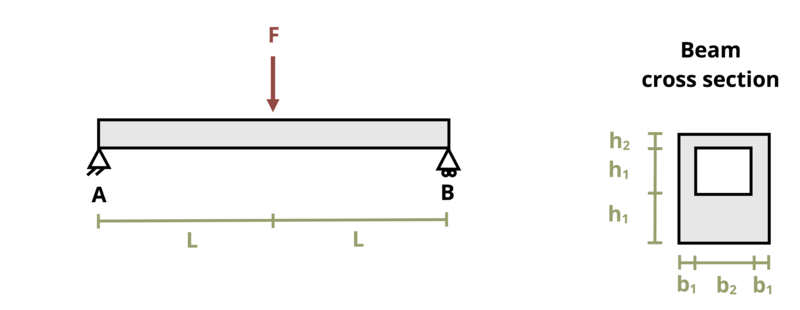
\includegraphics[keepaspectratio]{images/343.png}}
{[}Problem adapted from © Kurt Gramoll CC BY NC-SA 4.0{]}

\begin{Shaded}
\begin{Highlighting}[]
\NormalTok{\#| standalone: true}
\NormalTok{\#| viewerHeight: 600}
\NormalTok{\#| components: [viewer]}

\NormalTok{from shiny import App, render, ui, reactive}
\NormalTok{import random}
\NormalTok{import asyncio}
\NormalTok{import io}
\NormalTok{import math}
\NormalTok{import string}
\NormalTok{from datetime import datetime}
\NormalTok{from pathlib import Path}

\NormalTok{def generate\_random\_letters(length):}
\NormalTok{    \# Generate a random string of letters of specified length}
\NormalTok{    return \textquotesingle{}\textquotesingle{}.join(random.choice(string.ascii\_lowercase) for \_ in range(length))  }

\NormalTok{problem\_ID="343"}
\NormalTok{b1=reactive.Value("\_\_")}
\NormalTok{b2=reactive.Value("\_\_")}
\NormalTok{h1=reactive.Value("\_\_")}
\NormalTok{h2=reactive.Value("\_\_")}
\NormalTok{F=reactive.Value("\_\_")}
\NormalTok{L=reactive.Value("\_\_")}
  
\NormalTok{attempts=["Timestamp,Attempt,Answer,Feedback\textbackslash{}n"]}

\NormalTok{app\_ui = ui.page\_fluid(}
\NormalTok{    \#ui.markdown("**Please enter your ID number from your instructor and click to generate your problem**"),}
\NormalTok{    \#ui.input\_text("ID","", placeholder="Enter ID Number Here"),}
\NormalTok{    \#ui.input\_action\_button("generate\_problem", "Generate Problem", class\_="btn{-}primary"),}
\NormalTok{    ui.markdown("**Problem Statement**"),}
\NormalTok{    ui.output\_ui("ui\_problem\_statement"),}
\NormalTok{    ui.input\_text("answer","Your Answer in units of MPa", placeholder="Please enter your answer"),}
\NormalTok{    ui.input\_action\_button("submit", "Check Answer", class\_="btn{-}primary"),}
\NormalTok{    \#ui.download\_button("download", "Download File to Submit", class\_="btn{-}success"),}
\NormalTok{)}

\NormalTok{def server(input, output, session):}
\NormalTok{    \# Initialize a counter for attempts}
\NormalTok{    attempt\_counter = reactive.Value(0)}

\NormalTok{    @output}
\NormalTok{    @render.ui}
\NormalTok{    def ui\_problem\_statement():}
\NormalTok{        randomize\_vars()}
\NormalTok{        return[ui.markdown(f"A beam has the cross{-}section shown, where b\textless{}sub\textgreater{}1\textless{}/sub\textgreater{} = \{b1()\} mm, b\textless{}sub\textgreater{}2\textless{}/sub\textgreater{} = \{b2()\} mm, h\textless{}sub\textgreater{}1\textless{}/sub\textgreater{} = \{h1()\} mm, and h\textless{}sub\textgreater{}2\textless{}/sub\textgreater{} = \{h2()\} mm. The beam is subjected to a concentrated load F = \{F()\} kN at its midpoint. If length L = \{L()\} m, determine the magnitude of the maximum bending stress in the beam.")]}
    
\NormalTok{    \#@reactive.Effect}
\NormalTok{    \#@reactive.event(input.generate\_problem)}
\NormalTok{    def randomize\_vars():}
\NormalTok{        random.seed(101)}
\NormalTok{        b1.set(random.randrange(10, 20, 1))}
\NormalTok{        b2.set((b1()*3))}
\NormalTok{        h1.set((b1()*2))}
\NormalTok{        h2.set(b1())}
\NormalTok{        F.set(random.randrange(20, 300, 1)/10)}
\NormalTok{        L.set(random.randrange(20, 100, 1)/10)}
        
\NormalTok{    @reactive.Effect}
\NormalTok{    @reactive.event(input.submit)}
\NormalTok{    def \_():}
\NormalTok{        attempt\_counter.set(attempt\_counter() + 1)  \# Increment the attempt counter on each submission.}
\NormalTok{        Ay = F()/2}
\NormalTok{        M = Ay*L()}
\NormalTok{        A1 = (2*h1()+h2())*(2*b1()+b2())}
\NormalTok{        y1 = (2*h1()+h2())/2}
\NormalTok{        A2 = h1()*b2()}
\NormalTok{        y2 = 3*h1()/2}
\NormalTok{        yc = (A1*y1{-}A2*y2)/(A1{-}A2)}
\NormalTok{        I1 = ((2*b1()+b2())*(2*h1()+h2())**3)/12}
\NormalTok{        I2 = (b2()*h1()**3)/12}
\NormalTok{        Ic = ((I1+A1*(y1{-}yc)**2){-}(I2+A2*(y2{-}yc)**2))/(10**12)}
\NormalTok{        instr= (M*(2*h1()+h2(){-}yc)/Ic)/10**6}
\NormalTok{        if math.isclose(float(input.answer()), instr, rel\_tol=0.01):}
\NormalTok{            check = "*Correct*"}
\NormalTok{            correct\_indicator = "JL"}
\NormalTok{        else:}
\NormalTok{            check = "*Not Correct.*"}
\NormalTok{            correct\_indicator = "JG"}

\NormalTok{        \# Generate random parts for the encoded attempt.}
\NormalTok{        random\_start = generate\_random\_letters(4)}
\NormalTok{        random\_middle = generate\_random\_letters(4)}
\NormalTok{        random\_end = generate\_random\_letters(4)}
\NormalTok{        \#encoded\_attempt = f"\{random\_start\}\{problem\_ID\}{-}\{random\_middle\}\{attempt\_counter()\}\{correct\_indicator\}{-}\{random\_end\}\{input.ID()\}"}

\NormalTok{        \# Store the most recent encoded attempt in a reactive value so it persists across submissions}
\NormalTok{        \#session.encoded\_attempt = reactive.Value(encoded\_attempt)}

\NormalTok{        \# Append the attempt data to the attempts list without the encoded attempt}
\NormalTok{        attempts.append(f"\{datetime.now()\}, \{attempt\_counter()\}, \{input.answer()\}, \{check\}\textbackslash{}n")}

\NormalTok{        \# Show feedback to the user.}
\NormalTok{        feedback = ui.markdown(f"Your answer of \{input.answer()\} is \{check\}.")}
\NormalTok{        m = ui.modal(}
\NormalTok{            feedback,}
\NormalTok{            title="Feedback",}
\NormalTok{            easy\_close=True}
\NormalTok{        )}
\NormalTok{        ui.modal\_show(m)}

\NormalTok{    \#@render.download(filename=lambda: f"Problem\_Log{-}\{problem\_ID\}{-}\{input.ID()\}.csv")}
\NormalTok{    async def download():}
\NormalTok{        \# Start the CSV with the encoded attempt (without label)}
\NormalTok{        final\_encoded = session.encoded\_attempt() if session.encoded\_attempt is not None else "No attempts"}
\NormalTok{        yield f"\{final\_encoded\}\textbackslash{}n\textbackslash{}n"}
        
\NormalTok{        \# Write the header for the remaining CSV data once}
\NormalTok{        yield "Timestamp,Attempt,Answer,Feedback\textbackslash{}n"}
        
\NormalTok{        \# Write the attempts data, ensure that the header from the attempts list is not written again}
\NormalTok{        for attempt in attempts[1:]:  \# Skip the first element which is the header}
\NormalTok{            await asyncio.sleep(0.25)  \# This delay may not be necessary; adjust as needed}
\NormalTok{            yield attempt}


\NormalTok{\# App installation}
\NormalTok{app = App(app\_ui, server)}
\end{Highlighting}
\end{Shaded}

\chapter*{Problem 9.3 - Bending
Stress}\label{problem-9.3---bending-stress}
\addcontentsline{toc}{chapter}{Problem 9.3 - Bending Stress}

\markboth{Problem 9.3 - Bending Stress}{Problem 9.3 - Bending Stress}

\begin{figure}[H]

{\centering \pandocbounded{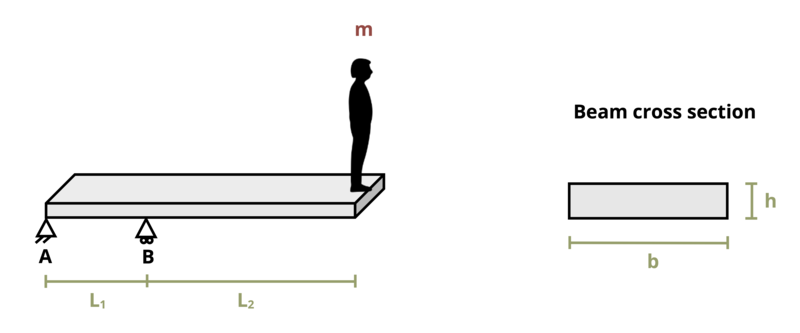
\includegraphics[keepaspectratio]{images/344.png}}

}

\caption{Figure 1: A diving board with a person standing on it.}

\end{figure}%

{[}Problem adapted from © Kurt Gramoll CC BY NC-SA 4.0{]}

\begin{Shaded}
\begin{Highlighting}[]
\NormalTok{\#| standalone: true}
\NormalTok{\#| viewerHeight: 600}
\NormalTok{\#| components: [viewer]}

\NormalTok{from shiny import App, render, ui, reactive}
\NormalTok{import random}
\NormalTok{import asyncio}
\NormalTok{import io}
\NormalTok{import math}
\NormalTok{import string}
\NormalTok{from datetime import datetime}
\NormalTok{from pathlib import Path}

\NormalTok{def generate\_random\_letters(length):}
\NormalTok{    \# Generate a random string of letters of specified length}
\NormalTok{    return \textquotesingle{}\textquotesingle{}.join(random.choice(string.ascii\_lowercase) for \_ in range(length))  }

\NormalTok{problem\_ID="344"}
\NormalTok{ma=reactive.Value("\_\_")}
\NormalTok{h=reactive.Value("\_\_")}
\NormalTok{b=reactive.Value("\_\_")}
\NormalTok{L1=reactive.Value("\_\_")}
\NormalTok{L2=reactive.Value("\_\_")}
\NormalTok{g = 9.81}

\NormalTok{attempts=["Timestamp,Attempt,Answer,Feedback\textbackslash{}n"]}

\NormalTok{app\_ui = ui.page\_fluid(}
\NormalTok{    \#ui.markdown("**Please enter your ID number from your instructor and click to generate your problem**"),}
\NormalTok{    \#ui.input\_text("ID","", placeholder="Enter ID Number Here"),}
\NormalTok{    \#ui.input\_action\_button("generate\_problem", "Generate Problem", class\_="btn{-}primary"),}
\NormalTok{    ui.markdown("**Problem Statement**"),}
\NormalTok{    ui.output\_ui("ui\_problem\_statement"),}
\NormalTok{    ui.input\_text("answer","Your Answer in units of MPa", placeholder="Please enter your answer"),}
\NormalTok{    ui.input\_action\_button("submit", "Check Answer", class\_="btn{-}primary"),}
\NormalTok{    \#ui.download\_button("download", "Download File to Submit", class\_="btn{-}success"),}
\NormalTok{)}

\NormalTok{def server(input, output, session):}
\NormalTok{    \# Initialize a counter for attempts}
\NormalTok{    attempt\_counter = reactive.Value(0)}

\NormalTok{    @output}
\NormalTok{    @render.ui}
\NormalTok{    def ui\_problem\_statement():}
\NormalTok{        randomize\_vars()}
\NormalTok{        return[ui.markdown(f"A person of mass m = \{ma()\} kg stands on the end of a diving board with cross{-}section b = \{b()\} mm and h = \{h()\} mm. If lengths L\textless{}sub\textgreater{}1\textless{}/sub\textgreater{} = \{L1()\} m and L\textless{}sub\textgreater{}2\textless{}/sub\textgreater{} = \{L2()\} m, determine the maximum bending stress in the board. Assume g = 9.81 m/s\textless{}sup\textgreater{}2\textless{}/sup\textgreater{}.")]}
    
\NormalTok{    \#@reactive.Effect}
\NormalTok{    \#@reactive.event(input.generate\_problem)}
\NormalTok{    def randomize\_vars():}
\NormalTok{        random.seed(101)}
\NormalTok{        ma.set(random.randrange(55, 100, 1))}
\NormalTok{        h.set(random.randrange(30, 60, 1))}
\NormalTok{        b.set((h()*6))}
\NormalTok{        L1.set(random.randrange(10, 30, 1)/10)}
\NormalTok{        L2.set(L1()*2)}
        
\NormalTok{    @reactive.Effect}
\NormalTok{    @reactive.event(input.submit)}
\NormalTok{    def \_():}
\NormalTok{        attempt\_counter.set(attempt\_counter() + 1)  \# Increment the attempt counter on each submission.}
\NormalTok{        Mo = float(ma())*L2()*g}
\NormalTok{        ytop = h()/2000}
\NormalTok{        I = ((b()/1000)*((h()/1000)**3))/12}
\NormalTok{        instr= float(Mo)*ytop/I/10**6}
\NormalTok{        if math.isclose(float(input.answer()), instr, rel\_tol=0.01):}
\NormalTok{            check = "*Correct*"}
\NormalTok{            correct\_indicator = "JL"}
\NormalTok{        else:}
\NormalTok{            check = "*Not Correct.*"}
\NormalTok{            correct\_indicator = "JG"}

\NormalTok{        \# Generate random parts for the encoded attempt.}
\NormalTok{        random\_start = generate\_random\_letters(4)}
\NormalTok{        random\_middle = generate\_random\_letters(4)}
\NormalTok{        random\_end = generate\_random\_letters(4)}
\NormalTok{        \#encoded\_attempt = f"\{random\_start\}\{problem\_ID\}{-}\{random\_middle\}\{attempt\_counter()\}\{correct\_indicator\}{-}\{random\_end\}\{input.ID()\}"}

\NormalTok{        \# Store the most recent encoded attempt in a reactive value so it persists across submissions}
\NormalTok{        \#session.encoded\_attempt = reactive.Value(encoded\_attempt)}

\NormalTok{        \# Append the attempt data to the attempts list without the encoded attempt}
\NormalTok{        attempts.append(f"\{datetime.now()\}, \{attempt\_counter()\}, \{input.answer()\}, \{check\}\textbackslash{}n")}

\NormalTok{        \# Show feedback to the user.}
\NormalTok{        feedback = ui.markdown(f"Your answer of \{input.answer()\} is \{check\}.")}
\NormalTok{        m = ui.modal(}
\NormalTok{            feedback,}
\NormalTok{            title="Feedback",}
\NormalTok{            easy\_close=True}
\NormalTok{        )}
\NormalTok{        ui.modal\_show(m)}

\NormalTok{    \#@render.download(filename=lambda: f"Problem\_Log{-}\{problem\_ID\}{-}\{input.ID()\}.csv")}
\NormalTok{    async def download():}
\NormalTok{        \# Start the CSV with the encoded attempt (without label)}
\NormalTok{        final\_encoded = session.encoded\_attempt() if session.encoded\_attempt is not None else "No attempts"}
\NormalTok{        yield f"\{final\_encoded\}\textbackslash{}n\textbackslash{}n"}
        
\NormalTok{        \# Write the header for the remaining CSV data once}
\NormalTok{        yield "Timestamp,Attempt,Answer,Feedback\textbackslash{}n"}
        
\NormalTok{        \# Write the attempts data, ensure that the header from the attempts list is not written again}
\NormalTok{        for attempt in attempts[1:]:  \# Skip the first element which is the header}
\NormalTok{            await asyncio.sleep(0.25)  \# This delay may not be necessary; adjust as needed}
\NormalTok{            yield attempt}


\NormalTok{\# App installation}
\NormalTok{app = App(app\_ui, server)}
\end{Highlighting}
\end{Shaded}

\chapter*{Problem 9.4 - Bending
Stress}\label{problem-9.4---bending-stress}
\addcontentsline{toc}{chapter}{Problem 9.4 - Bending Stress}

\markboth{Problem 9.4 - Bending Stress}{Problem 9.4 - Bending Stress}

\pandocbounded{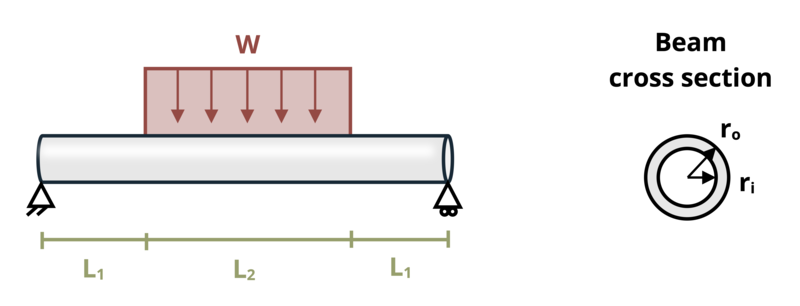
\includegraphics[keepaspectratio]{images/345.png}}
{[}Problem adapted from © Kurt Gramoll CC BY NC-SA 4.0{]}

\begin{Shaded}
\begin{Highlighting}[]
\NormalTok{\#| standalone: true}
\NormalTok{\#| viewerHeight: 600}
\NormalTok{\#| components: [viewer]}

\NormalTok{from shiny import App, render, ui, reactive}
\NormalTok{import random}
\NormalTok{import asyncio}
\NormalTok{import io}
\NormalTok{import math}
\NormalTok{import string}
\NormalTok{from datetime import datetime}
\NormalTok{from pathlib import Path}

\NormalTok{def generate\_random\_letters(length):}
\NormalTok{    \# Generate a random string of letters of specified length}
\NormalTok{    return \textquotesingle{}\textquotesingle{}.join(random.choice(string.ascii\_lowercase) for \_ in range(length))  }

\NormalTok{problem\_ID="345"}
\NormalTok{ro=reactive.Value("\_\_")}
\NormalTok{ri=reactive.Value("\_\_")}
\NormalTok{w=reactive.Value("\_\_")}
\NormalTok{L1=reactive.Value("\_\_")}
\NormalTok{L2=reactive.Value("\_\_")}

\NormalTok{attempts=["Timestamp,Attempt,Answer,Feedback\textbackslash{}n"]}

\NormalTok{app\_ui = ui.page\_fluid(}
\NormalTok{    \#ui.markdown("**Please enter your ID number from your instructor and click to generate your problem**"),}
\NormalTok{    \#ui.input\_text("ID","", placeholder="Enter ID Number Here"),}
\NormalTok{    \#ui.input\_action\_button("generate\_problem", "Generate Problem", class\_="btn{-}primary"),}
\NormalTok{    ui.markdown("**Problem Statement**"),}
\NormalTok{    ui.output\_ui("ui\_problem\_statement"),}
\NormalTok{    ui.input\_text("answer","Your Answer in units of psi", placeholder="Please enter your answer"),}
\NormalTok{    ui.input\_action\_button("submit", "Check Answer", class\_="btn{-}primary"),}
\NormalTok{    \#ui.download\_button("download", "Download File to Submit", class\_="btn{-}success"),}
\NormalTok{)}

\NormalTok{def server(input, output, session):}
\NormalTok{    \# Initialize a counter for attempts}
\NormalTok{    attempt\_counter = reactive.Value(0)}

\NormalTok{    @output}
\NormalTok{    @render.ui}
\NormalTok{    def ui\_problem\_statement():}
\NormalTok{        randomize\_vars()}
\NormalTok{        return[ui.markdown(f"A beam with a hollow circular cross{-}section of outer radius r\textless{}sub\textgreater{}o\textless{}/sub\textgreater{} = \{ro()\} in. and inner radius r\textless{}sub\textgreater{}i\textless{}/sub\textgreater{} = \{ri()\} in. is subjected to a distributed load as shown. If w = \{w()\} lb/ft, L\textless{}sub\textgreater{}1\textless{}/sub\textgreater{} = \{L1()\} ft, and L\textless{}sub\textgreater{}2\textless{}/sub\textgreater{} = \{L2()\} ft, determine the magnitude of the maximum bending stress in the beam.")]}
    
\NormalTok{    \#@reactive.Effect}
\NormalTok{    \#@reactive.event(input.generate\_problem)}
\NormalTok{    def randomize\_vars():}
\NormalTok{        random.seed(101)}
\NormalTok{        ro.set(random.randrange(40, 100, 1)/10)}
\NormalTok{        ri.set(ro(){-}random.randrange(5, 10, 1)/10)}
\NormalTok{        ri.set(round(ri(),1))}
\NormalTok{        w.set(random.randrange(100, 800, 10))}
\NormalTok{        L1.set(random.randrange(30, 100, 1)/10)}
\NormalTok{        L2.set(L1()*2)}
        
\NormalTok{    @reactive.Effect}
\NormalTok{    @reactive.event(input.submit)}
\NormalTok{    def \_():}
\NormalTok{        attempt\_counter.set(attempt\_counter() + 1)  \# Increment the attempt counter on each submission.}
\NormalTok{        R = w()*float(L2())/2}
\NormalTok{        M = {-}R*(L1()+L2()/2)+w()*L2()**2/8}
\NormalTok{        I = math.pi*(ro()**4{-}ri()**4)/4}
\NormalTok{        instr= abs(M*ro()*12/I)}
\NormalTok{        if math.isclose(float(input.answer()), instr, rel\_tol=0.01):}
\NormalTok{            check = "*Correct*"}
\NormalTok{            correct\_indicator = "JL"}
\NormalTok{        else:}
\NormalTok{            check = "*Not Correct.*"}
\NormalTok{            correct\_indicator = "JG"}

\NormalTok{        \# Generate random parts for the encoded attempt.}
\NormalTok{        random\_start = generate\_random\_letters(4)}
\NormalTok{        random\_middle = generate\_random\_letters(4)}
\NormalTok{        random\_end = generate\_random\_letters(4)}
\NormalTok{        \#encoded\_attempt = f"\{random\_start\}\{problem\_ID\}{-}\{random\_middle\}\{attempt\_counter()\}\{correct\_indicator\}{-}\{random\_end\}\{input.ID()\}"}

\NormalTok{        \# Store the most recent encoded attempt in a reactive value so it persists across submissions}
\NormalTok{        \#session.encoded\_attempt = reactive.Value(encoded\_attempt)}

\NormalTok{        \# Append the attempt data to the attempts list without the encoded attempt}
\NormalTok{        attempts.append(f"\{datetime.now()\}, \{attempt\_counter()\}, \{input.answer()\}, \{check\}\textbackslash{}n")}

\NormalTok{        \# Show feedback to the user.}
\NormalTok{        feedback = ui.markdown(f"Your answer of \{input.answer()\} is \{check\}.")}
\NormalTok{        m = ui.modal(}
\NormalTok{            feedback,}
\NormalTok{            title="Feedback",}
\NormalTok{            easy\_close=True}
\NormalTok{        )}
\NormalTok{        ui.modal\_show(m)}

\NormalTok{    \#@render.download(filename=lambda: f"Problem\_Log{-}\{problem\_ID\}{-}\{input.ID()\}.csv")}
\NormalTok{    async def download():}
\NormalTok{        \# Start the CSV with the encoded attempt (without label)}
\NormalTok{        final\_encoded = session.encoded\_attempt() if session.encoded\_attempt is not None else "No attempts"}
\NormalTok{        yield f"\{final\_encoded\}\textbackslash{}n\textbackslash{}n"}
        
\NormalTok{        \# Write the header for the remaining CSV data once}
\NormalTok{        yield "Timestamp,Attempt,Answer,Feedback\textbackslash{}n"}
        
\NormalTok{        \# Write the attempts data, ensure that the header from the attempts list is not written again}
\NormalTok{        for attempt in attempts[1:]:  \# Skip the first element which is the header}
\NormalTok{            await asyncio.sleep(0.25)  \# This delay may not be necessary; adjust as needed}
\NormalTok{            yield attempt}

\NormalTok{\# App installation}
\NormalTok{app = App(app\_ui, server)}
\end{Highlighting}
\end{Shaded}

\chapter*{Problem 9.5 - Bending
Stress}\label{problem-9.5---bending-stress}
\addcontentsline{toc}{chapter}{Problem 9.5 - Bending Stress}

\markboth{Problem 9.5 - Bending Stress}{Problem 9.5 - Bending Stress}

\begin{figure}[H]

{\centering \pandocbounded{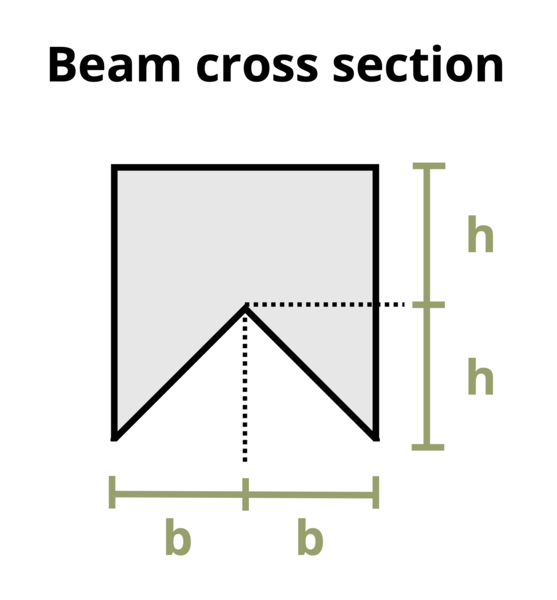
\includegraphics[keepaspectratio]{images/346.png}}

}

\caption{Figure 1: The cross section of a beam.}

\end{figure}%

{[}Problem adapted from © Kurt Gramoll CC BY NC-SA 4.0{]}

\begin{Shaded}
\begin{Highlighting}[]
\NormalTok{\#| standalone: true}
\NormalTok{\#| viewerHeight: 600}
\NormalTok{\#| components: [viewer]}

\NormalTok{from shiny import App, render, ui, reactive}
\NormalTok{import random}
\NormalTok{import asyncio}
\NormalTok{import io}
\NormalTok{import math}
\NormalTok{import string}
\NormalTok{from datetime import datetime}
\NormalTok{from pathlib import Path}

\NormalTok{def generate\_random\_letters(length):}
\NormalTok{    \# Generate a random string of letters of specified length}
\NormalTok{    return \textquotesingle{}\textquotesingle{}.join(random.choice(string.ascii\_lowercase) for \_ in range(length))  }

\NormalTok{problem\_ID="346"}
\NormalTok{b=reactive.Value("\_\_")}
\NormalTok{h=reactive.Value("\_\_")}
\NormalTok{M=reactive.Value("\_\_")}

\NormalTok{attempts=["Timestamp,Attempt,Answer,Feedback\textbackslash{}n"]}

\NormalTok{app\_ui = ui.page\_fluid(}
\NormalTok{    \#ui.markdown("**Please enter your ID number from your instructor and click to generate your problem**"),}
\NormalTok{    \#ui.input\_text("ID","", placeholder="Enter ID Number Here"),}
\NormalTok{    \#ui.input\_action\_button("generate\_problem", "Generate Problem", class\_="btn{-}primary"),}
\NormalTok{    ui.markdown("**Problem Statement**"),}
\NormalTok{    ui.output\_ui("ui\_problem\_statement"),}
\NormalTok{    ui.input\_text("answer","Your Answer in units of ksi", placeholder="Please enter your answer"),}
\NormalTok{    ui.input\_action\_button("submit", "Check Answer", class\_="btn{-}primary"),}
\NormalTok{    \#ui.download\_button("download", "Download File to Submit", class\_="btn{-}success"),}
\NormalTok{)}

\NormalTok{def server(input, output, session):}
\NormalTok{    \# Initialize a counter for attempts}
\NormalTok{    attempt\_counter = reactive.Value(0)}

\NormalTok{    @output}
\NormalTok{    @render.ui}
\NormalTok{    def ui\_problem\_statement():}
\NormalTok{        randomize\_vars()}
\NormalTok{        return[ui.markdown(f"A beam has the cross{-}section shown where b = \{b()\} in. and h = \{h()\} in. If the cross{-}section is subjected to an internal bending moment of \{M()\} kip{-}in, determine the magnitude of the bending stress at the bottom of the cross{-}section.")]}
    
\NormalTok{    \#@reactive.Effect}
\NormalTok{    \#@reactive.event(input.generate\_problem)}
\NormalTok{    def randomize\_vars():}
\NormalTok{        random.seed(101)}
\NormalTok{        b.set(random.randrange(20, 50, 1)/10)}
\NormalTok{        h.set(b())}
\NormalTok{        M.set(random.randrange(5, 100, 1))}
        
\NormalTok{    @reactive.Effect}
\NormalTok{    @reactive.event(input.submit)}
\NormalTok{    def \_():}
\NormalTok{        attempt\_counter.set(attempt\_counter() + 1)  \# Increment the attempt counter on each submission.}
\NormalTok{        y = 11*h()/9}
\NormalTok{        I = (2*b()*h()**3/12)+(2*b()*h()*(3*h()/2{-}y)**2)+(b()*h()**3/18)+(b()*h()*(2*h()/3{-}y)**2)}
\NormalTok{        instr= M()*y/I}
\NormalTok{        if math.isclose(float(input.answer()), instr, rel\_tol=0.01):}
\NormalTok{            check = "*Correct*"}
\NormalTok{            correct\_indicator = "JL"}
\NormalTok{        else:}
\NormalTok{            check = "*Not Correct.*"}
\NormalTok{            correct\_indicator = "JG"}

\NormalTok{        \# Generate random parts for the encoded attempt.}
\NormalTok{        random\_start = generate\_random\_letters(4)}
\NormalTok{        random\_middle = generate\_random\_letters(4)}
\NormalTok{        random\_end = generate\_random\_letters(4)}
\NormalTok{        \#encoded\_attempt = f"\{random\_start\}\{problem\_ID\}{-}\{random\_middle\}\{attempt\_counter()\}\{correct\_indicator\}{-}\{random\_end\}\{input.ID()\}"}

\NormalTok{        \# Store the most recent encoded attempt in a reactive value so it persists across submissions}
\NormalTok{        \#session.encoded\_attempt = reactive.Value(encoded\_attempt)}

\NormalTok{        \# Append the attempt data to the attempts list without the encoded attempt}
\NormalTok{        attempts.append(f"\{datetime.now()\}, \{attempt\_counter()\}, \{input.answer()\}, \{check\}\textbackslash{}n")}

\NormalTok{        \# Show feedback to the user.}
\NormalTok{        feedback = ui.markdown(f"Your answer of \{input.answer()\} is \{check\}.")}
\NormalTok{        m = ui.modal(}
\NormalTok{            feedback,}
\NormalTok{            title="Feedback",}
\NormalTok{            easy\_close=True}
\NormalTok{        )}
\NormalTok{        ui.modal\_show(m)}

\NormalTok{    \#@render.download(filename=lambda: f"Problem\_Log{-}\{problem\_ID\}{-}\{input.ID()\}.csv")}
\NormalTok{    async def download():}
\NormalTok{        \# Start the CSV with the encoded attempt (without label)}
\NormalTok{        final\_encoded = session.encoded\_attempt() if session.encoded\_attempt is not None else "No attempts"}
\NormalTok{        yield f"\{final\_encoded\}\textbackslash{}n\textbackslash{}n"}
        
\NormalTok{        \# Write the header for the remaining CSV data once}
\NormalTok{        yield "Timestamp,Attempt,Answer,Feedback\textbackslash{}n"}
        
\NormalTok{        \# Write the attempts data, ensure that the header from the attempts list is not written again}
\NormalTok{        for attempt in attempts[1:]:  \# Skip the first element which is the header}
\NormalTok{            await asyncio.sleep(0.25)  \# This delay may not be necessary; adjust as needed}
\NormalTok{            yield attempt}


\NormalTok{\# App installation}
\NormalTok{app = App(app\_ui, server)}
\end{Highlighting}
\end{Shaded}

\chapter*{Problem 9.6 - Bending
Stress}\label{problem-9.6---bending-stress}
\addcontentsline{toc}{chapter}{Problem 9.6 - Bending Stress}

\markboth{Problem 9.6 - Bending Stress}{Problem 9.6 - Bending Stress}

\pandocbounded{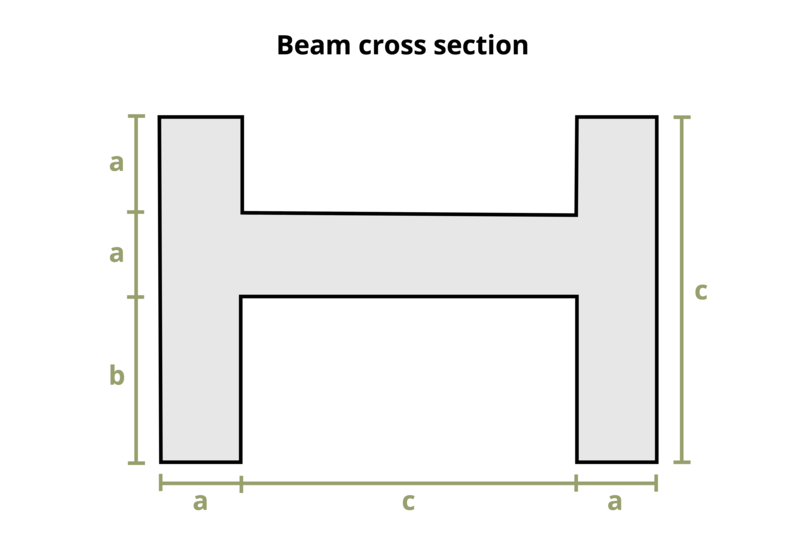
\includegraphics[keepaspectratio]{images/348.png}}
{[}Problem adapted from © Kurt Gramoll CC BY NC-SA 4.0{]}

\begin{Shaded}
\begin{Highlighting}[]
\NormalTok{\#| standalone: true}
\NormalTok{\#| viewerHeight: 600}
\NormalTok{\#| components: [viewer]}

\NormalTok{from shiny import App, render, ui, reactive}
\NormalTok{import random}
\NormalTok{import asyncio}
\NormalTok{import io}
\NormalTok{import math}
\NormalTok{import string}
\NormalTok{from datetime import datetime}
\NormalTok{from pathlib import Path}

\NormalTok{def generate\_random\_letters(length):}
\NormalTok{    \# Generate a random string of letters of specified length}
\NormalTok{    return \textquotesingle{}\textquotesingle{}.join(random.choice(string.ascii\_lowercase) for \_ in range(length))  }

\NormalTok{problem\_ID="348"}
\NormalTok{a=reactive.Value("\_\_")}
\NormalTok{b=reactive.Value("\_\_")}
\NormalTok{c=reactive.Value("\_\_")}
\NormalTok{M=reactive.Value("\_\_")}
  
\NormalTok{attempts=["Timestamp,Attempt,Answer,Feedback\textbackslash{}n"]}

\NormalTok{app\_ui = ui.page\_fluid(}
\NormalTok{    \#ui.markdown("**Please enter your ID number from your instructor and click to generate your problem**"),}
\NormalTok{    \#ui.input\_text("ID","", placeholder="Enter ID Number Here"),}
\NormalTok{    \#ui.input\_action\_button("generate\_problem", "Generate Problem", class\_="btn{-}primary"),}
\NormalTok{    ui.markdown("**Problem Statement**"),}
\NormalTok{    ui.output\_ui("ui\_problem\_statement"),}
\NormalTok{    ui.input\_text("answer","Your Answer in units of ksi", placeholder="Please enter your answer"),}
\NormalTok{    ui.input\_action\_button("submit", "Check Answer", class\_="btn{-}primary"),}
\NormalTok{    \#ui.download\_button("download", "Download File to Submit", class\_="btn{-}success"),}
\NormalTok{)}

\NormalTok{def server(input, output, session):}
\NormalTok{    \# Initialize a counter for attempts}
\NormalTok{    attempt\_counter = reactive.Value(0)}

\NormalTok{    @output}
\NormalTok{    @render.ui}
\NormalTok{    def ui\_problem\_statement():}
\NormalTok{        randomize\_vars()}
\NormalTok{        return[ui.markdown(f"A beam has the cross{-}section shown, where lengths a = \{a()\} in., b = \{b()\} in., and c = \{c()\} in. If the cross{-}section is subjected to an internal bending moment M = \{M()\} kip{-}in., determine the maximum bending stress.")]}
    
\NormalTok{    \#@reactive.Effect}
\NormalTok{    \#@reactive.event(input.generate\_problem)}
\NormalTok{    def randomize\_vars():}
\NormalTok{        random.seed(101)}
\NormalTok{        a.set(random.randrange(10,50,1)/10)}
\NormalTok{        b.set(a()*2)}
\NormalTok{        c.set(a()*4)}
\NormalTok{        M.set(random.randrange(10,100,1))}
        
\NormalTok{    @reactive.Effect}
\NormalTok{    @reactive.event(input.submit)}
\NormalTok{    def \_():}
\NormalTok{        attempt\_counter.set(attempt\_counter() + 1)  \# Increment the attempt counter on each submission.}
\NormalTok{        A = c()*a()}
\NormalTok{        h1 = c()/2}
\NormalTok{        h2 = a()/2+b()}
\NormalTok{        h = (A*h1*2+A*h2)/(3*A)}
\NormalTok{        I1 = a()*c()**3/12}
\NormalTok{        I2 = c()*a()**3/12}
\NormalTok{        y1 = h{-}h1}
\NormalTok{        y2 = h2{-}h}
\NormalTok{        I = 2*(I1+A*y1**2)+I2+A*y2**2}
\NormalTok{        instr= M()*h/I}
\NormalTok{        if math.isclose(float(input.answer()), instr, rel\_tol=0.01):}
\NormalTok{            check = "*Correct*"}
\NormalTok{            correct\_indicator = "JL"}
\NormalTok{        else:}
\NormalTok{            check = "*Not Correct.*"}
\NormalTok{            correct\_indicator = "JG"}

\NormalTok{        \# Generate random parts for the encoded attempt.}
\NormalTok{        random\_start = generate\_random\_letters(4)}
\NormalTok{        random\_middle = generate\_random\_letters(4)}
\NormalTok{        random\_end = generate\_random\_letters(4)}
\NormalTok{        \#encoded\_attempt = f"\{random\_start\}\{problem\_ID\}{-}\{random\_middle\}\{attempt\_counter()\}\{correct\_indicator\}{-}\{random\_end\}\{input.ID()\}"}

\NormalTok{        \# Store the most recent encoded attempt in a reactive value so it persists across submissions}
\NormalTok{        \#session.encoded\_attempt = reactive.Value(encoded\_attempt)}

\NormalTok{        \# Append the attempt data to the attempts list without the encoded attempt}
\NormalTok{        attempts.append(f"\{datetime.now()\}, \{attempt\_counter()\}, \{input.answer()\}, \{check\}\textbackslash{}n")}

\NormalTok{        \# Show feedback to the user.}
\NormalTok{        feedback = ui.markdown(f"Your answer of \{input.answer()\} is \{check\}.")}
\NormalTok{        m = ui.modal(}
\NormalTok{            feedback,}
\NormalTok{            title="Feedback",}
\NormalTok{            easy\_close=True}
\NormalTok{        )}
\NormalTok{        ui.modal\_show(m)}

\NormalTok{    \#@render.download(filename=lambda: f"Problem\_Log{-}\{problem\_ID\}{-}\{input.ID()\}.csv")}
\NormalTok{    async def download():}
\NormalTok{        \# Start the CSV with the encoded attempt (without label)}
\NormalTok{        final\_encoded = session.encoded\_attempt() if session.encoded\_attempt is not None else "No attempts"}
\NormalTok{        yield f"\{final\_encoded\}\textbackslash{}n\textbackslash{}n"}
        
\NormalTok{        \# Write the header for the remaining CSV data once}
\NormalTok{        yield "Timestamp,Attempt,Answer,Feedback\textbackslash{}n"}
        
\NormalTok{        \# Write the attempts data, ensure that the header from the attempts list is not written again}
\NormalTok{        for attempt in attempts[1:]:  \# Skip the first element which is the header}
\NormalTok{            await asyncio.sleep(0.25)  \# This delay may not be necessary; adjust as needed}
\NormalTok{            yield attempt}

\NormalTok{\# App installation}
\NormalTok{app = App(app\_ui, server)}
\end{Highlighting}
\end{Shaded}

\chapter*{Problem 9.7 - Bending
Stress}\label{problem-9.7---bending-stress}
\addcontentsline{toc}{chapter}{Problem 9.7 - Bending Stress}

\markboth{Problem 9.7 - Bending Stress}{Problem 9.7 - Bending Stress}

\pandocbounded{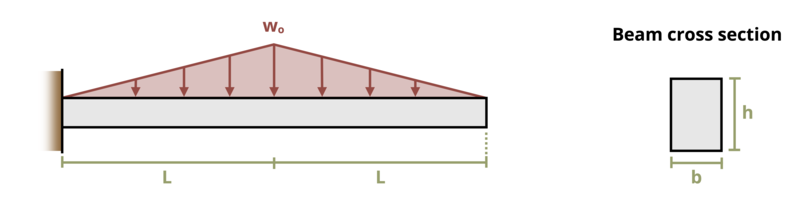
\includegraphics[keepaspectratio]{images/349.png}}
{[}Problem adapted from © Kurt Gramoll CC BY NC-SA 4.0{]}

\begin{Shaded}
\begin{Highlighting}[]
\NormalTok{\#| standalone: true}
\NormalTok{\#| viewerHeight: 600}
\NormalTok{\#| components: [viewer]}

\NormalTok{from shiny import App, render, ui, reactive}
\NormalTok{import random}
\NormalTok{import asyncio}
\NormalTok{import io}
\NormalTok{import math}
\NormalTok{import string}
\NormalTok{from datetime import datetime}
\NormalTok{from pathlib import Path}

\NormalTok{def generate\_random\_letters(length):}
\NormalTok{    \# Generate a random string of letters of specified length}
\NormalTok{    return \textquotesingle{}\textquotesingle{}.join(random.choice(string.ascii\_lowercase) for \_ in range(length))  }

\NormalTok{problem\_ID="349"}
\NormalTok{b=reactive.Value("\_\_")}
\NormalTok{h=reactive.Value("\_\_")}
\NormalTok{w0=reactive.Value("\_\_")}
\NormalTok{L=reactive.Value("\_\_")}
  
\NormalTok{attempts=["Timestamp,Attempt,Answer,Feedback\textbackslash{}n"]}

\NormalTok{app\_ui = ui.page\_fluid(}
\NormalTok{    \#ui.markdown("**Please enter your ID number from your instructor and click to generate your problem**"),}
\NormalTok{    \#ui.input\_text("ID","", placeholder="Enter ID Number Here"),}
\NormalTok{    \#ui.input\_action\_button("generate\_problem", "Generate Problem", class\_="btn{-}primary"),}
\NormalTok{    ui.markdown("**Problem Statement**"),}
\NormalTok{    ui.output\_ui("ui\_problem\_statement"),}
\NormalTok{    ui.input\_text("answer","Your Answer in units of ksi", placeholder="Please enter your answer"),}
\NormalTok{    ui.input\_action\_button("submit", "Check Answer", class\_="btn{-}primary"),}
\NormalTok{    \#ui.download\_button("download", "Download File to Submit", class\_="btn{-}success"),}
\NormalTok{)}

\NormalTok{def server(input, output, session):}
\NormalTok{    \# Initialize a counter for attempts}
\NormalTok{    attempt\_counter = reactive.Value(0)}

\NormalTok{    @output}
\NormalTok{    @render.ui}
\NormalTok{    def ui\_problem\_statement():}
\NormalTok{        randomize\_vars()}
\NormalTok{        return[ui.markdown(f"A beam with a rectangular cross{-}section of base b = \{b()\} in. and height h = \{h()\} in. is subjected to the loading shown. If w\textless{}sub\textgreater{}o\textless{}/sub\textgreater{} = \{w0()\} lb/ft and L = \{L()\} ft, determine the maximum bending stress in the beam.")]}
    
\NormalTok{    \#@reactive.Effect}
\NormalTok{    \#@reactive.event(input.generate\_problem)}
\NormalTok{    def randomize\_vars():}
\NormalTok{        random.seed(101)}
\NormalTok{        b.set(random.randrange(10,50,1)/10)}
\NormalTok{        h.set(b()*2)}
\NormalTok{        w0.set(random.randrange(500,1500,10))}
\NormalTok{        L.set(random.randrange(20,60,1)/10)}
        
\NormalTok{    @reactive.Effect}
\NormalTok{    @reactive.event(input.submit)}
\NormalTok{    def \_():}
\NormalTok{        attempt\_counter.set(attempt\_counter() + 1)  \# Increment the attempt counter on each submission.}
\NormalTok{        M = w0()*L()/2*L()*12*2/3+(L()*12+L()*12*2/3)*w0()*L()/2}
\NormalTok{        I = b()*h()**3/12}
\NormalTok{        instr= M*h()/2/I/1000}
\NormalTok{        if math.isclose(float(input.answer()), instr, rel\_tol=0.01):}
\NormalTok{            check = "*Correct*"}
\NormalTok{            correct\_indicator = "JL"}
\NormalTok{        else:}
\NormalTok{            check = "*Not Correct.*"}
\NormalTok{            correct\_indicator = "JG"}

\NormalTok{        \# Generate random parts for the encoded attempt.}
\NormalTok{        random\_start = generate\_random\_letters(4)}
\NormalTok{        random\_middle = generate\_random\_letters(4)}
\NormalTok{        random\_end = generate\_random\_letters(4)}
\NormalTok{        \#encoded\_attempt = f"\{random\_start\}\{problem\_ID\}{-}\{random\_middle\}\{attempt\_counter()\}\{correct\_indicator\}{-}\{random\_end\}\{input.ID()\}"}

\NormalTok{        \# Store the most recent encoded attempt in a reactive value so it persists across submissions}
\NormalTok{        \#session.encoded\_attempt = reactive.Value(encoded\_attempt)}

\NormalTok{        \# Append the attempt data to the attempts list without the encoded attempt}
\NormalTok{        attempts.append(f"\{datetime.now()\}, \{attempt\_counter()\}, \{input.answer()\}, \{check\}\textbackslash{}n")}

\NormalTok{        \# Show feedback to the user.}
\NormalTok{        feedback = ui.markdown(f"Your answer of \{input.answer()\} is \{check\}.")}
\NormalTok{        m = ui.modal(}
\NormalTok{            feedback,}
\NormalTok{            title="Feedback",}
\NormalTok{            easy\_close=True}
\NormalTok{        )}
\NormalTok{        ui.modal\_show(m)}

\NormalTok{    \#@render.download(filename=lambda: f"Problem\_Log{-}\{problem\_ID\}{-}\{input.ID()\}.csv")}
\NormalTok{    async def download():}
\NormalTok{        \# Start the CSV with the encoded attempt (without label)}
\NormalTok{        final\_encoded = session.encoded\_attempt() if session.encoded\_attempt is not None else "No attempts"}
\NormalTok{        yield f"\{final\_encoded\}\textbackslash{}n\textbackslash{}n"}
        
\NormalTok{        \# Write the header for the remaining CSV data once}
\NormalTok{        yield "Timestamp,Attempt,Answer,Feedback\textbackslash{}n"}
        
\NormalTok{        \# Write the attempts data, ensure that the header from the attempts list is not written again}
\NormalTok{        for attempt in attempts[1:]:  \# Skip the first element which is the header}
\NormalTok{            await asyncio.sleep(0.25)  \# This delay may not be necessary; adjust as needed}
\NormalTok{            yield attempt}

\NormalTok{\# App installation}
\NormalTok{app = App(app\_ui, server)}
\end{Highlighting}
\end{Shaded}

\chapter*{Problem 9.8 - Bending
Stress}\label{problem-9.8---bending-stress}
\addcontentsline{toc}{chapter}{Problem 9.8 - Bending Stress}

\markboth{Problem 9.8 - Bending Stress}{Problem 9.8 - Bending Stress}

\pandocbounded{\includegraphics[keepaspectratio]{images/351.png}}
{[}Problem adapted from © Kurt Gramoll CC BY NC-SA 4.0{]}

\begin{Shaded}
\begin{Highlighting}[]
\NormalTok{\#| standalone: true}
\NormalTok{\#| viewerHeight: 600}
\NormalTok{\#| components: [viewer]}

\NormalTok{from shiny import App, render, ui, reactive}
\NormalTok{import random}
\NormalTok{import asyncio}
\NormalTok{import io}
\NormalTok{import math}
\NormalTok{import string}
\NormalTok{from datetime import datetime}
\NormalTok{from pathlib import Path}

\NormalTok{def generate\_random\_letters(length):}
\NormalTok{    \# Generate a random string of letters of specified length}
\NormalTok{    return \textquotesingle{}\textquotesingle{}.join(random.choice(string.ascii\_lowercase) for \_ in range(length))  }

\NormalTok{problem\_ID="350"}
\NormalTok{t=reactive.Value("\_\_")}
\NormalTok{w=reactive.Value("\_\_")}
\NormalTok{h=reactive.Value("\_\_")}
\NormalTok{M=reactive.Value("\_\_")}
  
\NormalTok{attempts=["Timestamp,Attempt,Answer,Feedback\textbackslash{}n"]}

\NormalTok{app\_ui = ui.page\_fluid(}
\NormalTok{    \#ui.markdown("**Please enter your ID number from your instructor and click to generate your problem**"),}
\NormalTok{    \#ui.input\_text("ID","", placeholder="Enter ID Number Here"),}
\NormalTok{    \#ui.input\_action\_button("generate\_problem", "Generate Problem", class\_="btn{-}primary"),}
\NormalTok{    ui.markdown("**Problem Statement**"),}
\NormalTok{    ui.output\_ui("ui\_problem\_statement"),}
\NormalTok{    ui.input\_text("answer","Your Answer", placeholder="Please enter your answer"),}
\NormalTok{    ui.input\_action\_button("submit", "Check Answer", class\_="btn{-}primary"),}
\NormalTok{    \#ui.download\_button("download", "Download File to Submit", class\_="btn{-}success"),}
\NormalTok{)}

\NormalTok{def server(input, output, session):}
\NormalTok{    \# Initialize a counter for attempts}
\NormalTok{    attempt\_counter = reactive.Value(0)}

\NormalTok{    @output}
\NormalTok{    @render.ui}
\NormalTok{    def ui\_problem\_statement():}
\NormalTok{        randomize\_vars()}
\NormalTok{        return[ui.markdown(f"A beam has the cross{-}section shown, where t = \{t()\} mm, w = \{w()\} mm, and h = \{h()\} mm. If the cross{-}section is subjected to internal bending moment M = \{M()\} kN{-}m, determine the ratio of the maximum bending stress at the top of the beam to the maximum bending stress at the bottom.")]}
    
\NormalTok{    \#@reactive.Effect}
\NormalTok{    \#@reactive.event(input.generate\_problem)}
\NormalTok{    def randomize\_vars():}
\NormalTok{        random.seed(101)}
\NormalTok{        t.set(random.randrange(20,40,1))}
\NormalTok{        w.set(t()+random.randrange(20,30,1))}
\NormalTok{        h.set(w()+random.randrange(10,20,1))}
\NormalTok{        M.set(random.randrange(10,50,1))}
        
\NormalTok{    @reactive.Effect}
\NormalTok{    @reactive.event(input.submit)}
\NormalTok{    def \_():}
\NormalTok{        attempt\_counter.set(attempt\_counter() + 1)  \# Increment the attempt counter on each submission.}
\NormalTok{        A1 = (2*w()+t())*t()}
\NormalTok{        A2 = h()*t()}
\NormalTok{        y1 = h()+t()/2}
\NormalTok{        y2 = h()/2}
\NormalTok{        ybar = A1*y1+A2*y2/(A1+A2)}
\NormalTok{        top = h()+t(){-}ybar}
\NormalTok{        instr= top/ybar}
\NormalTok{        if math.isclose(float(input.answer()), instr, rel\_tol=0.01):}
\NormalTok{            check = "*Correct*"}
\NormalTok{            correct\_indicator = "JL"}
\NormalTok{        else:}
\NormalTok{            check = "*Not Correct.*"}
\NormalTok{            correct\_indicator = "JG"}

\NormalTok{        \# Generate random parts for the encoded attempt.}
\NormalTok{        random\_start = generate\_random\_letters(4)}
\NormalTok{        random\_middle = generate\_random\_letters(4)}
\NormalTok{        random\_end = generate\_random\_letters(4)}
\NormalTok{        \#encoded\_attempt = f"\{random\_start\}\{problem\_ID\}{-}\{random\_middle\}\{attempt\_counter()\}\{correct\_indicator\}{-}\{random\_end\}\{input.ID()\}"}

\NormalTok{        \# Store the most recent encoded attempt in a reactive value so it persists across submissions}
\NormalTok{        \#session.encoded\_attempt = reactive.Value(encoded\_attempt)}

\NormalTok{        \# Append the attempt data to the attempts list without the encoded attempt}
\NormalTok{        attempts.append(f"\{datetime.now()\}, \{attempt\_counter()\}, \{input.answer()\}, \{check\}\textbackslash{}n")}

\NormalTok{        \# Show feedback to the user.}
\NormalTok{        feedback = ui.markdown(f"Your answer of \{input.answer()\} is \{check\}.")}
\NormalTok{        m = ui.modal(}
\NormalTok{            feedback,}
\NormalTok{            title="Feedback",}
\NormalTok{            easy\_close=True}
\NormalTok{        )}
\NormalTok{        ui.modal\_show(m)}

\NormalTok{    \#@render.download(filename=lambda: f"Problem\_Log{-}\{problem\_ID\}{-}\{input.ID()\}.csv")}
\NormalTok{    async def download():}
\NormalTok{        \# Start the CSV with the encoded attempt (without label)}
\NormalTok{        final\_encoded = session.encoded\_attempt() if session.encoded\_attempt is not None else "No attempts"}
\NormalTok{        yield f"\{final\_encoded\}\textbackslash{}n\textbackslash{}n"}
        
\NormalTok{        \# Write the header for the remaining CSV data once}
\NormalTok{        yield "Timestamp,Attempt,Answer,Feedback\textbackslash{}n"}
        
\NormalTok{        \# Write the attempts data, ensure that the header from the attempts list is not written again}
\NormalTok{        for attempt in attempts[1:]:  \# Skip the first element which is the header}
\NormalTok{            await asyncio.sleep(0.25)  \# This delay may not be necessary; adjust as needed}
\NormalTok{            yield attempt}

\NormalTok{\# App installation}
\NormalTok{app = App(app\_ui, server)}
\end{Highlighting}
\end{Shaded}

\chapter*{Problem 9.9 - Bending
Stress}\label{problem-9.9---bending-stress}
\addcontentsline{toc}{chapter}{Problem 9.9 - Bending Stress}

\markboth{Problem 9.9 - Bending Stress}{Problem 9.9 - Bending Stress}

\pandocbounded{\includegraphics[keepaspectratio]{images/350.png}}
{[}Problem adapted from © Kurt Gramoll CC BY NC-SA 4.0{]}

\begin{Shaded}
\begin{Highlighting}[]
\NormalTok{\#| standalone: true}
\NormalTok{\#| viewerHeight: 600}
\NormalTok{\#| components: [viewer]}

\NormalTok{from shiny import App, render, ui, reactive}
\NormalTok{import random}
\NormalTok{import asyncio}
\NormalTok{import io}
\NormalTok{import math}
\NormalTok{import string}
\NormalTok{from datetime import datetime}
\NormalTok{from pathlib import Path}

\NormalTok{def generate\_random\_letters(length):}
\NormalTok{    \# Generate a random string of letters of specified length}
\NormalTok{    return \textquotesingle{}\textquotesingle{}.join(random.choice(string.ascii\_lowercase) for \_ in range(length))  }

\NormalTok{problem\_ID="351"}
\NormalTok{L=reactive.Value("\_\_")}
\NormalTok{r=reactive.Value("\_\_")}
\NormalTok{w=reactive.Value("\_\_")}
  
\NormalTok{attempts=["Timestamp,Attempt,Answer,Feedback\textbackslash{}n"]}

\NormalTok{app\_ui = ui.page\_fluid(}
\NormalTok{    \#ui.markdown("**Please enter your ID number from your instructor and click to generate your problem**"),}
\NormalTok{    \#ui.input\_text("ID","", placeholder="Enter ID Number Here"),}
\NormalTok{    \#ui.input\_action\_button("generate\_problem", "Generate Problem", class\_="btn{-}primary"),}
\NormalTok{    ui.markdown("**Problem Statement**"),}
\NormalTok{    ui.output\_ui("ui\_problem\_statement"),}
\NormalTok{    ui.input\_text("answer","Your Answer in units of MPa", placeholder="Please enter your answer"),}
\NormalTok{    ui.input\_action\_button("submit", "Check Answer", class\_="btn{-}primary"),}
\NormalTok{    \#ui.download\_button("download", "Download File to Submit", class\_="btn{-}success"),}
\NormalTok{)}

\NormalTok{def server(input, output, session):}
\NormalTok{    \# Initialize a counter for attempts}
\NormalTok{    attempt\_counter = reactive.Value(0)}

\NormalTok{    @output}
\NormalTok{    @render.ui}
\NormalTok{    def ui\_problem\_statement():}
\NormalTok{        randomize\_vars()}
\NormalTok{        return[ui.markdown(f"A beam of length L = \{L()\} m has a circular cross{-}section of radius r = \{r()\} mm. The beam is subjected to distributed load w = \{w()\} kN/m as shown. Determine the maximum bending stress in the beam.")]}
    
\NormalTok{    \#@reactive.Effect}
\NormalTok{    \#@reactive.event(input.generate\_problem)}
\NormalTok{    def randomize\_vars():}
\NormalTok{        random.seed(101)}
\NormalTok{        L.set(random.randrange(40,100,1)/10)}
\NormalTok{        r.set(random.randrange(30,100,1))}
\NormalTok{        w.set(random.randrange(10,50,1)/10)}
        
\NormalTok{    @reactive.Effect}
\NormalTok{    @reactive.event(input.submit)}
\NormalTok{    def \_():}
\NormalTok{        attempt\_counter.set(attempt\_counter() + 1)  \# Increment the attempt counter on each submission.}
\NormalTok{        Ay = w()*L()*L()/2/L()}
\NormalTok{        M = Ay*L()/2{-}w()*L()/2*L()/2/2}
\NormalTok{        I = math.pi*(r()/1000)**4/4}
\NormalTok{        instr= M*r()/1000/I/1000}
\NormalTok{        if math.isclose(float(input.answer()), instr, rel\_tol=0.01):}
\NormalTok{            check = "*Correct*"}
\NormalTok{            correct\_indicator = "JL"}
\NormalTok{        else:}
\NormalTok{            check = "*Not Correct.*"}
\NormalTok{            correct\_indicator = "JG"}

\NormalTok{        \# Generate random parts for the encoded attempt.}
\NormalTok{        random\_start = generate\_random\_letters(4)}
\NormalTok{        random\_middle = generate\_random\_letters(4)}
\NormalTok{        random\_end = generate\_random\_letters(4)}
\NormalTok{        \#encoded\_attempt = f"\{random\_start\}\{problem\_ID\}{-}\{random\_middle\}\{attempt\_counter()\}\{correct\_indicator\}{-}\{random\_end\}\{input.ID()\}"}

\NormalTok{        \# Store the most recent encoded attempt in a reactive value so it persists across submissions}
\NormalTok{        \#session.encoded\_attempt = reactive.Value(encoded\_attempt)}

\NormalTok{        \# Append the attempt data to the attempts list without the encoded attempt}
\NormalTok{        attempts.append(f"\{datetime.now()\}, \{attempt\_counter()\}, \{input.answer()\}, \{check\}\textbackslash{}n")}

\NormalTok{        \# Show feedback to the user.}
\NormalTok{        feedback = ui.markdown(f"Your answer of \{input.answer()\} is \{check\}.")}
\NormalTok{        m = ui.modal(}
\NormalTok{            feedback,}
\NormalTok{            title="Feedback",}
\NormalTok{            easy\_close=True}
\NormalTok{        )}
\NormalTok{        ui.modal\_show(m)}

\NormalTok{    \#@render.download(filename=lambda: f"Problem\_Log{-}\{problem\_ID\}{-}\{input.ID()\}.csv")}
\NormalTok{    async def download():}
\NormalTok{        \# Start the CSV with the encoded attempt (without label)}
\NormalTok{        final\_encoded = session.encoded\_attempt() if session.encoded\_attempt is not None else "No attempts"}
\NormalTok{        yield f"\{final\_encoded\}\textbackslash{}n\textbackslash{}n"}
        
\NormalTok{        \# Write the header for the remaining CSV data once}
\NormalTok{        yield "Timestamp,Attempt,Answer,Feedback\textbackslash{}n"}
        
\NormalTok{        \# Write the attempts data, ensure that the header from the attempts list is not written again}
\NormalTok{        for attempt in attempts[1:]:  \# Skip the first element which is the header}
\NormalTok{            await asyncio.sleep(0.25)  \# This delay may not be necessary; adjust as needed}
\NormalTok{            yield attempt}

\NormalTok{\# App installation}
\NormalTok{app = App(app\_ui, server)}
\end{Highlighting}
\end{Shaded}

\chapter*{Problem 9.10 - Bending
Stress}\label{problem-9.10---bending-stress}
\addcontentsline{toc}{chapter}{Problem 9.10 - Bending Stress}

\markboth{Problem 9.10 - Bending Stress}{Problem 9.10 - Bending Stress}

\pandocbounded{\includegraphics[keepaspectratio]{images/352.png}}
{[}Problem adapted from © Kurt Gramoll CC BY NC-SA 4.0{]}

\begin{Shaded}
\begin{Highlighting}[]
\NormalTok{\#| standalone: true}
\NormalTok{\#| viewerHeight: 600}
\NormalTok{\#| components: [viewer]}

\NormalTok{from shiny import App, render, ui, reactive}
\NormalTok{import random}
\NormalTok{import asyncio}
\NormalTok{import io}
\NormalTok{import math}
\NormalTok{import string}
\NormalTok{from datetime import datetime}
\NormalTok{from pathlib import Path}

\NormalTok{def generate\_random\_letters(length):}
\NormalTok{    \# Generate a random string of letters of specified length}
\NormalTok{    return \textquotesingle{}\textquotesingle{}.join(random.choice(string.ascii\_lowercase) for \_ in range(length))  }

\NormalTok{problem\_ID="352"}
\NormalTok{a=reactive.Value("\_\_")}
\NormalTok{b=reactive.Value("\_\_")}
\NormalTok{c=reactive.Value("\_\_")}
\NormalTok{M=reactive.Value("\_\_")}
  
\NormalTok{attempts=["Timestamp,Attempt,Answer,Feedback\textbackslash{}n"]}

\NormalTok{app\_ui = ui.page\_fluid(}
\NormalTok{    \#ui.markdown("**Please enter your ID number from your instructor and click to generate your problem**"),}
\NormalTok{    \#ui.input\_text("ID","", placeholder="Enter ID Number Here"),}
\NormalTok{    \#ui.input\_action\_button("generate\_problem", "Generate Problem", class\_="btn{-}primary"),}
\NormalTok{    ui.markdown("**Problem Statement**"),}
\NormalTok{    ui.output\_ui("ui\_problem\_statement"),}
\NormalTok{    ui.input\_text("answer","Your Answer in units of MPa", placeholder="Please enter your answer"),}
\NormalTok{    ui.input\_action\_button("submit", "Check Answer", class\_="btn{-}primary"),}
\NormalTok{    \#ui.download\_button("download", "Download File to Submit", class\_="btn{-}success"),}
\NormalTok{)}

\NormalTok{def server(input, output, session):}
\NormalTok{    \# Initialize a counter for attempts}
\NormalTok{    attempt\_counter = reactive.Value(0)}

\NormalTok{    @output}
\NormalTok{    @render.ui}
\NormalTok{    def ui\_problem\_statement():}
\NormalTok{        randomize\_vars()}
\NormalTok{        return[ui.markdown(f"A beam has the cross{-}section shown, where dimensions a = \{a()\} mm, b = \{b()\} mm, and c = \{c()\} mm. The internal bending moment on this cross{-}section is M = \{M()\} kN{-}m. Determine the bending stress at point A.")]}
    
\NormalTok{    \#@reactive.Effect}
\NormalTok{    \#@reactive.event(input.generate\_problem)}
\NormalTok{    def randomize\_vars():}
\NormalTok{        random.seed(101)}
\NormalTok{        a.set(random.randrange(30,80,1))}
\NormalTok{        b.set(a()*2)}
\NormalTok{        c.set(a()*3)}
\NormalTok{        M.set(random.randrange(10,200,1)/10)}
        
\NormalTok{    @reactive.Effect}
\NormalTok{    @reactive.event(input.submit)}
\NormalTok{    def \_():}
\NormalTok{        attempt\_counter.set(attempt\_counter() + 1)  \# Increment the attempt counter on each submission.}
\NormalTok{        A1 = c()/1000*a()/1000}
\NormalTok{        A2 = (a()/1000)**2}
\NormalTok{        A3 = b()/1000*a()/1000}
\NormalTok{        y1 = 2*a()/1000+a()/2000}
\NormalTok{        y2 = a()/1000+a()/2000}
\NormalTok{        y3 = a()/2000}
\NormalTok{        ybar = A1*y1+A2*y2+A3*y3/(A1+A2+A3)}
\NormalTok{        I1 = (a()/1000)**3*c()/12000+A1*(y1{-}ybar)**2}
\NormalTok{        I2 = (a()/1000)**3*a()/12000+A2*(y2{-}ybar)**2}
\NormalTok{        I3 = (a()/1000)**3*b()/12000+A3*(y3{-}ybar)**2}
\NormalTok{        I = I1+I2+I3}
\NormalTok{        instr= M()*ybar/I}
\NormalTok{        if math.isclose(float(input.answer()), instr, rel\_tol=0.01):}
\NormalTok{            check = "*Correct*"}
\NormalTok{            correct\_indicator = "JL"}
\NormalTok{        else:}
\NormalTok{            check = "*Not Correct.*"}
\NormalTok{            correct\_indicator = "JG"}

\NormalTok{        \# Generate random parts for the encoded attempt.}
\NormalTok{        random\_start = generate\_random\_letters(4)}
\NormalTok{        random\_middle = generate\_random\_letters(4)}
\NormalTok{        random\_end = generate\_random\_letters(4)}
\NormalTok{        \#encoded\_attempt = f"\{random\_start\}\{problem\_ID\}{-}\{random\_middle\}\{attempt\_counter()\}\{correct\_indicator\}{-}\{random\_end\}\{input.ID()\}"}

\NormalTok{        \# Store the most recent encoded attempt in a reactive value so it persists across submissions}
\NormalTok{        \#session.encoded\_attempt = reactive.Value(encoded\_attempt)}

\NormalTok{        \# Append the attempt data to the attempts list without the encoded attempt}
\NormalTok{        attempts.append(f"\{datetime.now()\}, \{attempt\_counter()\}, \{input.answer()\}, \{check\}\textbackslash{}n")}

\NormalTok{        \# Show feedback to the user.}
\NormalTok{        feedback = ui.markdown(f"Your answer of \{input.answer()\} is \{check\}.")}
\NormalTok{        m = ui.modal(}
\NormalTok{            feedback,}
\NormalTok{            title="Feedback",}
\NormalTok{            easy\_close=True}
\NormalTok{        )}
\NormalTok{        ui.modal\_show(m)}

\NormalTok{    \#@render.download(filename=lambda: f"Problem\_Log{-}\{problem\_ID\}{-}\{input.ID()\}.csv")}
\NormalTok{    async def download():}
\NormalTok{        \# Start the CSV with the encoded attempt (without label)}
\NormalTok{        final\_encoded = session.encoded\_attempt() if session.encoded\_attempt is not None else "No attempts"}
\NormalTok{        yield f"\{final\_encoded\}\textbackslash{}n\textbackslash{}n"}
        
\NormalTok{        \# Write the header for the remaining CSV data once}
\NormalTok{        yield "Timestamp,Attempt,Answer,Feedback\textbackslash{}n"}
        
\NormalTok{        \# Write the attempts data, ensure that the header from the attempts list is not written again}
\NormalTok{        for attempt in attempts[1:]:  \# Skip the first element which is the header}
\NormalTok{            await asyncio.sleep(0.25)  \# This delay may not be necessary; adjust as needed}
\NormalTok{            yield attempt}

\NormalTok{\# App installation}
\NormalTok{app = App(app\_ui, server)}
\end{Highlighting}
\end{Shaded}

\chapter*{Problem 9.11 - Bending
Stress}\label{problem-9.11---bending-stress}
\addcontentsline{toc}{chapter}{Problem 9.11 - Bending Stress}

\markboth{Problem 9.11 - Bending Stress}{Problem 9.11 - Bending Stress}

\pandocbounded{\includegraphics[keepaspectratio]{images/353.png}}
{[}Problem adapted from © Kurt Gramoll CC BY NC-SA 4.0{]}

\begin{Shaded}
\begin{Highlighting}[]
\NormalTok{\#| standalone: true}
\NormalTok{\#| viewerHeight: 600}
\NormalTok{\#| components: [viewer]}

\NormalTok{from shiny import App, render, ui, reactive}
\NormalTok{import random}
\NormalTok{import asyncio}
\NormalTok{import io}
\NormalTok{import math}
\NormalTok{import string}
\NormalTok{from datetime import datetime}
\NormalTok{from pathlib import Path}

\NormalTok{def generate\_random\_letters(length):}
\NormalTok{    \# Generate a random string of letters of specified length}
\NormalTok{    return \textquotesingle{}\textquotesingle{}.join(random.choice(string.ascii\_lowercase) for \_ in range(length))  }

\NormalTok{problem\_ID="353"}
\NormalTok{w=reactive.Value("\_\_")}
\NormalTok{F=reactive.Value("\_\_")}
  
\NormalTok{attempts=["Timestamp,Attempt,Answer,Feedback\textbackslash{}n"]}

\NormalTok{app\_ui = ui.page\_fluid(}
\NormalTok{    \#ui.markdown("**Please enter your ID number from your instructor and click to generate your problem**"),}
\NormalTok{    \#ui.input\_text("ID","", placeholder="Enter ID Number Here"),}
\NormalTok{    \#ui.input\_action\_button("generate\_problem", "Generate Problem", class\_="btn{-}primary"),}
\NormalTok{    ui.markdown("**Problem Statement**"),}
\NormalTok{    ui.output\_ui("ui\_problem\_statement"),}
\NormalTok{    ui.input\_text("answer","Your Answer in units of ksi", placeholder="Please enter your answer"),}
\NormalTok{    ui.input\_action\_button("submit", "Check Answer", class\_="btn{-}primary"),}
\NormalTok{    \#ui.download\_button("download", "Download File to Submit", class\_="btn{-}success"),}
\NormalTok{)}

\NormalTok{def server(input, output, session):}
\NormalTok{    \# Initialize a counter for attempts}
\NormalTok{    attempt\_counter = reactive.Value(0)}

\NormalTok{    @output}
\NormalTok{    @render.ui}
\NormalTok{    def ui\_problem\_statement():}
\NormalTok{        randomize\_vars()}
\NormalTok{        return[ui.markdown(f"A beam has the cross{-}section shown. If loads w = \{w()\} lb/in. and F = \{F()\} lb, determine the maximum bending stress in the beam.")]}
    
\NormalTok{    \#@reactive.Effect}
\NormalTok{    \#@reactive.event(input.generate\_problem)}
\NormalTok{    def randomize\_vars():}
\NormalTok{        random.seed(101)}
\NormalTok{        w.set(random.randrange(10,30,1))}
\NormalTok{        F.set(random.randrange(200,500,10))}
        
\NormalTok{    @reactive.Effect}
\NormalTok{    @reactive.event(input.submit)}
\NormalTok{    def \_():}
\NormalTok{        attempt\_counter.set(attempt\_counter() + 1)  \# Increment the attempt counter on each submission.}
\NormalTok{        M = w()*30*27+F()*54}
\NormalTok{        ybar = 1.1}
\NormalTok{        I = 7.233}
\NormalTok{        instr= M*ybar/I/1000}
\NormalTok{        if math.isclose(float(input.answer()), instr, rel\_tol=0.01):}
\NormalTok{            check = "*Correct*"}
\NormalTok{            correct\_indicator = "JL"}
\NormalTok{        else:}
\NormalTok{            check = "*Not Correct.*"}
\NormalTok{            correct\_indicator = "JG"}

\NormalTok{        \# Generate random parts for the encoded attempt.}
\NormalTok{        random\_start = generate\_random\_letters(4)}
\NormalTok{        random\_middle = generate\_random\_letters(4)}
\NormalTok{        random\_end = generate\_random\_letters(4)}
\NormalTok{        \#encoded\_attempt = f"\{random\_start\}\{problem\_ID\}{-}\{random\_middle\}\{attempt\_counter()\}\{correct\_indicator\}{-}\{random\_end\}\{input.ID()\}"}

\NormalTok{        \# Store the most recent encoded attempt in a reactive value so it persists across submissions}
\NormalTok{        \#session.encoded\_attempt = reactive.Value(encoded\_attempt)}

\NormalTok{        \# Append the attempt data to the attempts list without the encoded attempt}
\NormalTok{        attempts.append(f"\{datetime.now()\}, \{attempt\_counter()\}, \{input.answer()\}, \{check\}\textbackslash{}n")}

\NormalTok{        \# Show feedback to the user.}
\NormalTok{        feedback = ui.markdown(f"Your answer of \{input.answer()\} is \{check\}.")}
\NormalTok{        m = ui.modal(}
\NormalTok{            feedback,}
\NormalTok{            title="Feedback",}
\NormalTok{            easy\_close=True}
\NormalTok{        )}
\NormalTok{        ui.modal\_show(m)}

\NormalTok{    \#@render.download(filename=lambda: f"Problem\_Log{-}\{problem\_ID\}{-}\{input.ID()\}.csv")}
\NormalTok{    async def download():}
\NormalTok{        \# Start the CSV with the encoded attempt (without label)}
\NormalTok{        final\_encoded = session.encoded\_attempt() if session.encoded\_attempt is not None else "No attempts"}
\NormalTok{        yield f"\{final\_encoded\}\textbackslash{}n\textbackslash{}n"}
        
\NormalTok{        \# Write the header for the remaining CSV data once}
\NormalTok{        yield "Timestamp,Attempt,Answer,Feedback\textbackslash{}n"}
        
\NormalTok{        \# Write the attempts data, ensure that the header from the attempts list is not written again}
\NormalTok{        for attempt in attempts[1:]:  \# Skip the first element which is the header}
\NormalTok{            await asyncio.sleep(0.25)  \# This delay may not be necessary; adjust as needed}
\NormalTok{            yield attempt}

\NormalTok{\# App installation}
\NormalTok{app = App(app\_ui, server)}
\end{Highlighting}
\end{Shaded}

\chapter*{Problem 9.12 - Bending
Stress}\label{problem-9.12---bending-stress}
\addcontentsline{toc}{chapter}{Problem 9.12 - Bending Stress}

\markboth{Problem 9.12 - Bending Stress}{Problem 9.12 - Bending Stress}

\pandocbounded{\includegraphics[keepaspectratio]{images/354.png}}
{[}Problem adapted from © Kurt Gramoll CC BY NC-SA 4.0{]}

\begin{Shaded}
\begin{Highlighting}[]
\NormalTok{\#| standalone: true}
\NormalTok{\#| viewerHeight: 600}
\NormalTok{\#| components: [viewer]}

\NormalTok{from shiny import App, render, ui, reactive}
\NormalTok{import random}
\NormalTok{import asyncio}
\NormalTok{import io}
\NormalTok{import math}
\NormalTok{import string}
\NormalTok{from datetime import datetime}
\NormalTok{from pathlib import Path}

\NormalTok{def generate\_random\_letters(length):}
\NormalTok{    \# Generate a random string of letters of specified length}
\NormalTok{    return \textquotesingle{}\textquotesingle{}.join(random.choice(string.ascii\_lowercase) for \_ in range(length))  }

\NormalTok{problem\_ID="354"}
\NormalTok{h=reactive.Value("\_\_")}
\NormalTok{b=reactive.Value("\_\_")}
\NormalTok{w0=reactive.Value("\_\_")}
\NormalTok{M=reactive.Value("\_\_")}
  
\NormalTok{attempts=["Timestamp,Attempt,Answer,Feedback\textbackslash{}n"]}

\NormalTok{app\_ui = ui.page\_fluid(}
\NormalTok{    \#ui.markdown("**Please enter your ID number from your instructor and click to generate your problem**"),}
\NormalTok{    \#ui.input\_text("ID","", placeholder="Enter ID Number Here"),}
\NormalTok{    \#ui.input\_action\_button("generate\_problem", "Generate Problem", class\_="btn{-}primary"),}
\NormalTok{    ui.markdown("**Problem Statement**"),}
\NormalTok{    ui.output\_ui("ui\_problem\_statement"),}
\NormalTok{    ui.input\_text("answer","Your Answer in units of MPa", placeholder="Please enter your answer"),}
\NormalTok{    ui.input\_action\_button("submit", "Check Answer", class\_="btn{-}primary"),}
\NormalTok{    \#ui.download\_button("download", "Download File to Submit", class\_="btn{-}success"),}
\NormalTok{)}

\NormalTok{def server(input, output, session):}
\NormalTok{    \# Initialize a counter for attempts}
\NormalTok{    attempt\_counter = reactive.Value(0)}

\NormalTok{    @output}
\NormalTok{    @render.ui}
\NormalTok{    def ui\_problem\_statement():}
\NormalTok{        randomize\_vars()}
\NormalTok{        return[ui.markdown(f"A beam has the rectangular cross{-}section shown, where b = \{b()\} mm and h = \{h()\} mm. The beam is subjected to loads where w\textless{}sub\textgreater{}0\textless{}/sub\textgreater{} = \{w0()\} kN/m and M = \{M()\} kN{-}m. Determine the maximum bending stress in the beam.")]}
    
\NormalTok{    \#@reactive.Effect}
\NormalTok{    \#@reactive.event(input.generate\_problem)}
\NormalTok{    def randomize\_vars():}
\NormalTok{        random.seed(101)}
\NormalTok{        h.set(random.randrange(100,250,5))}
\NormalTok{        b.set(h()*2.5)}
\NormalTok{        w0.set(random.randrange(10,50,1)/10)}
\NormalTok{        M.set(random.randrange(20,50,1))}
        
\NormalTok{    @reactive.Effect}
\NormalTok{    @reactive.event(input.submit)}
\NormalTok{    def \_():}
\NormalTok{        attempt\_counter.set(attempt\_counter() + 1)  \# Increment the attempt counter on each submission.}
\NormalTok{        Mmax = w0()*6/2*4+M()}
\NormalTok{        I = b()/1000*(h()/1000)**3/12}
\NormalTok{        ybar = h()/2000}
\NormalTok{        instr= Mmax*ybar/I/1000}
\NormalTok{        if math.isclose(float(input.answer()), instr, rel\_tol=0.01):}
\NormalTok{            check = "*Correct*"}
\NormalTok{            correct\_indicator = "JL"}
\NormalTok{        else:}
\NormalTok{            check = "*Not Correct.*"}
\NormalTok{            correct\_indicator = "JG"}

\NormalTok{        \# Generate random parts for the encoded attempt.}
\NormalTok{        random\_start = generate\_random\_letters(4)}
\NormalTok{        random\_middle = generate\_random\_letters(4)}
\NormalTok{        random\_end = generate\_random\_letters(4)}
\NormalTok{        \#encoded\_attempt = f"\{random\_start\}\{problem\_ID\}{-}\{random\_middle\}\{attempt\_counter()\}\{correct\_indicator\}{-}\{random\_end\}\{input.ID()\}"}

\NormalTok{        \# Store the most recent encoded attempt in a reactive value so it persists across submissions}
\NormalTok{        \#session.encoded\_attempt = reactive.Value(encoded\_attempt)}

\NormalTok{        \# Append the attempt data to the attempts list without the encoded attempt}
\NormalTok{        attempts.append(f"\{datetime.now()\}, \{attempt\_counter()\}, \{input.answer()\}, \{check\}\textbackslash{}n")}

\NormalTok{        \# Show feedback to the user.}
\NormalTok{        feedback = ui.markdown(f"Your answer of \{input.answer()\} is \{check\}.")}
\NormalTok{        m = ui.modal(}
\NormalTok{            feedback,}
\NormalTok{            title="Feedback",}
\NormalTok{            easy\_close=True}
\NormalTok{        )}
\NormalTok{        ui.modal\_show(m)}

\NormalTok{    \#@render.download(filename=lambda: f"Problem\_Log{-}\{problem\_ID\}{-}\{input.ID()\}.csv")}
\NormalTok{    async def download():}
\NormalTok{        \# Start the CSV with the encoded attempt (without label)}
\NormalTok{        final\_encoded = session.encoded\_attempt() if session.encoded\_attempt is not None else "No attempts"}
\NormalTok{        yield f"\{final\_encoded\}\textbackslash{}n\textbackslash{}n"}
        
\NormalTok{        \# Write the header for the remaining CSV data once}
\NormalTok{        yield "Timestamp,Attempt,Answer,Feedback\textbackslash{}n"}
        
\NormalTok{        \# Write the attempts data, ensure that the header from the attempts list is not written again}
\NormalTok{        for attempt in attempts[1:]:  \# Skip the first element which is the header}
\NormalTok{            await asyncio.sleep(0.25)  \# This delay may not be necessary; adjust as needed}
\NormalTok{            yield attempt}

\NormalTok{\# App installation}
\NormalTok{app = App(app\_ui, server)}
\end{Highlighting}
\end{Shaded}

\chapter*{Problem 9.13 - Bending
Stress}\label{problem-9.13---bending-stress}
\addcontentsline{toc}{chapter}{Problem 9.13 - Bending Stress}

\markboth{Problem 9.13 - Bending Stress}{Problem 9.13 - Bending Stress}

\pandocbounded{\includegraphics[keepaspectratio]{images/355.png}}
{[}Problem adapted from © Kurt Gramoll CC BY NC-SA 4.0{]}

\begin{Shaded}
\begin{Highlighting}[]
\NormalTok{\#| standalone: true}
\NormalTok{\#| viewerHeight: 600}
\NormalTok{\#| components: [viewer]}

\NormalTok{from shiny import App, render, ui, reactive}
\NormalTok{import random}
\NormalTok{import asyncio}
\NormalTok{import io}
\NormalTok{import math}
\NormalTok{import string}
\NormalTok{from datetime import datetime}
\NormalTok{from pathlib import Path}

\NormalTok{def generate\_random\_letters(length):}
\NormalTok{    \# Generate a random string of letters of specified length}
\NormalTok{    return \textquotesingle{}\textquotesingle{}.join(random.choice(string.ascii\_lowercase) for \_ in range(length))  }

\NormalTok{problem\_ID="355"}
\NormalTok{ri=reactive.Value("\_\_")}
\NormalTok{ro=reactive.Value("\_\_")}
\NormalTok{offset=reactive.Value("\_\_")}
\NormalTok{M=reactive.Value("\_\_")}
  
\NormalTok{attempts=["Timestamp,Attempt,Answer,Feedback\textbackslash{}n"]}

\NormalTok{app\_ui = ui.page\_fluid(}
\NormalTok{    \#ui.markdown("**Please enter your ID number from your instructor and click to generate your problem**"),}
\NormalTok{    \#ui.input\_text("ID","", placeholder="Enter ID Number Here"),}
\NormalTok{    \#ui.input\_action\_button("generate\_problem", "Generate Problem", class\_="btn{-}primary"),}
\NormalTok{    ui.markdown("**Problem Statement**"),}
\NormalTok{    ui.output\_ui("ui\_problem\_statement"),}
\NormalTok{    ui.input\_text("answer","Your Answer in units of ksi", placeholder="Please enter your answer"),}
\NormalTok{    ui.input\_action\_button("submit", "Check Answer", class\_="btn{-}primary"),}
\NormalTok{    \#ui.download\_button("download", "Download File to Submit", class\_="btn{-}success"),}
\NormalTok{)}

\NormalTok{def server(input, output, session):}
\NormalTok{    \# Initialize a counter for attempts}
\NormalTok{    attempt\_counter = reactive.Value(0)}

\NormalTok{    @output}
\NormalTok{    @render.ui}
\NormalTok{    def ui\_problem\_statement():}
\NormalTok{        randomize\_vars()}
\NormalTok{        return[ui.markdown(f"A beam has the cross{-}section shown, where r\textless{}sub\textgreater{}o\textless{}/sub\textgreater{} = \{ro()\} in. and r\textless{}sub\textgreater{}i\textless{}/sub\textgreater{} = \{ri()\} in. The inner radius hollow center is offsest by ẟ = \{offset()\} in. Determine the bending stress at the bottom of the beam when it is subjected to an internal bending moment M = \{M()\} kip{-}ft.")]}
    
\NormalTok{    \#@reactive.Effect}
\NormalTok{    \#@reactive.event(input.generate\_problem)}
\NormalTok{    def randomize\_vars():}
\NormalTok{        random.seed(101)}
\NormalTok{        ri.set(random.randrange(20,60,1)/10)}
\NormalTok{        ro.set(ri()+random.randrange(20,30,1)/10)}
\NormalTok{        offset.set(round((ro(){-}ri())/2,1))}
\NormalTok{        M.set(random.randrange(25,100,1))}
        
\NormalTok{    @reactive.Effect}
\NormalTok{    @reactive.event(input.submit)}
\NormalTok{    def \_():}
\NormalTok{        attempt\_counter.set(attempt\_counter() + 1)  \# Increment the attempt counter on each submission.}
\NormalTok{        A1 = math.pi*ri()**2}
\NormalTok{        A2 = math.pi*ro()**2}
\NormalTok{        y1 = {-}ro(){-}offset()}
\NormalTok{        y2 = ro()}
\NormalTok{        ybar = (A1*y1+A2*y2)/(A1+A2)}
\NormalTok{        I1 = ri()**4*math.pi/4}
\NormalTok{        I2 = ro()**4*math.pi/4}
\NormalTok{        I = {-}I1{-}({-}y1{-}ybar)**2*A1+I2+(y2{-}ybar)**2*A2}
\NormalTok{        instr= M()*12*ybar/I}
\NormalTok{        if math.isclose(float(input.answer()), instr, rel\_tol=0.01):}
\NormalTok{            check = "*Correct*"}
\NormalTok{            correct\_indicator = "JL"}
\NormalTok{        else:}
\NormalTok{            check = "*Not Correct.*"}
\NormalTok{            correct\_indicator = "JG"}

\NormalTok{        \# Generate random parts for the encoded attempt.}
\NormalTok{        random\_start = generate\_random\_letters(4)}
\NormalTok{        random\_middle = generate\_random\_letters(4)}
\NormalTok{        random\_end = generate\_random\_letters(4)}
\NormalTok{        \#encoded\_attempt = f"\{random\_start\}\{problem\_ID\}{-}\{random\_middle\}\{attempt\_counter()\}\{correct\_indicator\}{-}\{random\_end\}\{input.ID()\}"}

\NormalTok{        \# Store the most recent encoded attempt in a reactive value so it persists across submissions}
\NormalTok{        \#session.encoded\_attempt = reactive.Value(encoded\_attempt)}

\NormalTok{        \# Append the attempt data to the attempts list without the encoded attempt}
\NormalTok{        attempts.append(f"\{datetime.now()\}, \{attempt\_counter()\}, \{input.answer()\}, \{check\}\textbackslash{}n")}

\NormalTok{        \# Show feedback to the user.}
\NormalTok{        feedback = ui.markdown(f"Your answer of \{input.answer()\} is \{check\}.")}
\NormalTok{        m = ui.modal(}
\NormalTok{            feedback,}
\NormalTok{            title="Feedback",}
\NormalTok{            easy\_close=True}
\NormalTok{        )}
\NormalTok{        ui.modal\_show(m)}

\NormalTok{    \#@render.download(filename=lambda: f"Problem\_Log{-}\{problem\_ID\}{-}\{input.ID()\}.csv")}
\NormalTok{    async def download():}
\NormalTok{        \# Start the CSV with the encoded attempt (without label)}
\NormalTok{        final\_encoded = session.encoded\_attempt() if session.encoded\_attempt is not None else "No attempts"}
\NormalTok{        yield f"\{final\_encoded\}\textbackslash{}n\textbackslash{}n"}
        
\NormalTok{        \# Write the header for the remaining CSV data once}
\NormalTok{        yield "Timestamp,Attempt,Answer,Feedback\textbackslash{}n"}
        
\NormalTok{        \# Write the attempts data, ensure that the header from the attempts list is not written again}
\NormalTok{        for attempt in attempts[1:]:  \# Skip the first element which is the header}
\NormalTok{            await asyncio.sleep(0.25)  \# This delay may not be necessary; adjust as needed}
\NormalTok{            yield attempt}

\NormalTok{\# App installation}
\NormalTok{app = App(app\_ui, server)}
\end{Highlighting}
\end{Shaded}

\chapter*{Problem 9.14 - Bending
Stress}\label{problem-9.14---bending-stress}
\addcontentsline{toc}{chapter}{Problem 9.14 - Bending Stress}

\markboth{Problem 9.14 - Bending Stress}{Problem 9.14 - Bending Stress}

\pandocbounded{\includegraphics[keepaspectratio]{images/356.png}}
{[}Problem adapted from © Kurt Gramoll CC BY NC-SA 4.0{]}

\begin{Shaded}
\begin{Highlighting}[]
\NormalTok{\#| standalone: true}
\NormalTok{\#| viewerHeight: 600}
\NormalTok{\#| components: [viewer]}

\NormalTok{from shiny import App, render, ui, reactive}
\NormalTok{import random}
\NormalTok{import asyncio}
\NormalTok{import io}
\NormalTok{import math}
\NormalTok{import string}
\NormalTok{from datetime import datetime}
\NormalTok{from pathlib import Path}

\NormalTok{def generate\_random\_letters(length):}
\NormalTok{    \# Generate a random string of letters of specified length}
\NormalTok{    return \textquotesingle{}\textquotesingle{}.join(random.choice(string.ascii\_lowercase) for \_ in range(length))  }

\NormalTok{problem\_ID="356"}
\NormalTok{F=reactive.Value("\_\_")}
\NormalTok{w=reactive.Value("\_\_")}
\NormalTok{L2=reactive.Value("\_\_")}
\NormalTok{L1=reactive.Value("\_\_")}
\NormalTok{L3=reactive.Value("\_\_")}
  
\NormalTok{attempts=["Timestamp,Attempt,Answer,Feedback\textbackslash{}n"]}

\NormalTok{app\_ui = ui.page\_fluid(}
\NormalTok{    \#ui.markdown("**Please enter your ID number from your instructor and click to generate your problem**"),}
\NormalTok{    \#ui.input\_text("ID","", placeholder="Enter ID Number Here"),}
\NormalTok{    \#ui.input\_action\_button("generate\_problem", "Generate Problem", class\_="btn{-}primary"),}
\NormalTok{    ui.markdown("**Problem Statement**"),}
\NormalTok{    ui.output\_ui("ui\_problem\_statement"),}
\NormalTok{    ui.input\_text("answer","Your Answer in units of ksi", placeholder="Please enter your answer"),}
\NormalTok{    ui.input\_action\_button("submit", "Check Answer", class\_="btn{-}primary"),}
\NormalTok{    \#ui.download\_button("download", "Download File to Submit", class\_="btn{-}success"),}
\NormalTok{)}

\NormalTok{def server(input, output, session):}
\NormalTok{    \# Initialize a counter for attempts}
\NormalTok{    attempt\_counter = reactive.Value(0)}

\NormalTok{    @output}
\NormalTok{    @render.ui}
\NormalTok{    def ui\_problem\_statement():}
\NormalTok{        randomize\_vars()}
\NormalTok{        return[ui.markdown(f"A wide flange section W14 x 30 is used to support the loads shown, where F = \{F()\} kips and w = \{w()\} kips/ft. If lengths L\textless{}sub\textgreater{}1\textless{}/sub\textgreater{} = \{L1()\} ft, L\textless{}sub\textgreater{}2\textless{}/sub\textgreater{} = \{L2()\} ft, and L\textless{}sub\textgreater{}3\textless{}/sub\textgreater{} = \{L3()\} ft, determine the maximum bending stress in the beam. Ignore the beam weight.")]}
    
\NormalTok{    \#@reactive.Effect}
\NormalTok{    \#@reactive.event(input.generate\_problem)}
\NormalTok{    def randomize\_vars():}
\NormalTok{        random.seed(101)}
\NormalTok{        F.set(random.randrange(10,100,1))}
\NormalTok{        w.set(random.randrange(100,300,1)/10)}
\NormalTok{        L2.set(random.randrange(10,25,1)/10)}
\NormalTok{        L1.set(L2()*2)}
\NormalTok{        L3.set(round(L2()*3,1))}
        
\NormalTok{    @reactive.Effect}
\NormalTok{    @reactive.event(input.submit)}
\NormalTok{    def \_():}
\NormalTok{        attempt\_counter.set(attempt\_counter() + 1)  \# Increment the attempt counter on each submission.}
\NormalTok{        M = F()*L1()}
\NormalTok{        instr= M*12/42}
\NormalTok{        if math.isclose(float(input.answer()), instr, rel\_tol=0.01):}
\NormalTok{            check = "*Correct*"}
\NormalTok{            correct\_indicator = "JL"}
\NormalTok{        else:}
\NormalTok{            check = "*Not Correct.*"}
\NormalTok{            correct\_indicator = "JG"}

\NormalTok{        \# Generate random parts for the encoded attempt.}
\NormalTok{        random\_start = generate\_random\_letters(4)}
\NormalTok{        random\_middle = generate\_random\_letters(4)}
\NormalTok{        random\_end = generate\_random\_letters(4)}
\NormalTok{        \#encoded\_attempt = f"\{random\_start\}\{problem\_ID\}{-}\{random\_middle\}\{attempt\_counter()\}\{correct\_indicator\}{-}\{random\_end\}\{input.ID()\}"}

\NormalTok{        \# Store the most recent encoded attempt in a reactive value so it persists across submissions}
\NormalTok{        \#session.encoded\_attempt = reactive.Value(encoded\_attempt)}

\NormalTok{        \# Append the attempt data to the attempts list without the encoded attempt}
\NormalTok{        attempts.append(f"\{datetime.now()\}, \{attempt\_counter()\}, \{input.answer()\}, \{check\}\textbackslash{}n")}

\NormalTok{        \# Show feedback to the user.}
\NormalTok{        feedback = ui.markdown(f"Your answer of \{input.answer()\} is \{check\}.")}
\NormalTok{        m = ui.modal(}
\NormalTok{            feedback,}
\NormalTok{            title="Feedback",}
\NormalTok{            easy\_close=True}
\NormalTok{        )}
\NormalTok{        ui.modal\_show(m)}

\NormalTok{    \#@render.download(filename=lambda: f"Problem\_Log{-}\{problem\_ID\}{-}\{input.ID()\}.csv")}
\NormalTok{    async def download():}
\NormalTok{        \# Start the CSV with the encoded attempt (without label)}
\NormalTok{        final\_encoded = session.encoded\_attempt() if session.encoded\_attempt is not None else "No attempts"}
\NormalTok{        yield f"\{final\_encoded\}\textbackslash{}n\textbackslash{}n"}
        
\NormalTok{        \# Write the header for the remaining CSV data once}
\NormalTok{        yield "Timestamp,Attempt,Answer,Feedback\textbackslash{}n"}
        
\NormalTok{        \# Write the attempts data, ensure that the header from the attempts list is not written again}
\NormalTok{        for attempt in attempts[1:]:  \# Skip the first element which is the header}
\NormalTok{            await asyncio.sleep(0.25)  \# This delay may not be necessary; adjust as needed}
\NormalTok{            yield attempt}

\NormalTok{\# App installation}
\NormalTok{app = App(app\_ui, server)}
\end{Highlighting}
\end{Shaded}

\chapter*{Problem 9.15 - Bending
Stress}\label{problem-9.15---bending-stress}
\addcontentsline{toc}{chapter}{Problem 9.15 - Bending Stress}

\markboth{Problem 9.15 - Bending Stress}{Problem 9.15 - Bending Stress}

\pandocbounded{\includegraphics[keepaspectratio]{images/358.png}}
{[}Problem adapted from © Kurt Gramoll CC BY NC-SA 4.0{]}

\begin{Shaded}
\begin{Highlighting}[]
\NormalTok{\#| standalone: true}
\NormalTok{\#| viewerHeight: 600}
\NormalTok{\#| components: [viewer]}

\NormalTok{from shiny import App, render, ui, reactive}
\NormalTok{import random}
\NormalTok{import asyncio}
\NormalTok{import io}
\NormalTok{import math}
\NormalTok{import string}
\NormalTok{from datetime import datetime}
\NormalTok{from pathlib import Path}

\NormalTok{def generate\_random\_letters(length):}
\NormalTok{    \# Generate a random string of letters of specified length}
\NormalTok{    return \textquotesingle{}\textquotesingle{}.join(random.choice(string.ascii\_lowercase) for \_ in range(length))  }

\NormalTok{problem\_ID="358"}
\NormalTok{ri=reactive.Value("\_\_")}
\NormalTok{ro=reactive.Value("\_\_")}
\NormalTok{w0=reactive.Value("\_\_")}
\NormalTok{F=reactive.Value("\_\_")}
  
\NormalTok{attempts=["Timestamp,Attempt,Answer,Feedback\textbackslash{}n"]}

\NormalTok{app\_ui = ui.page\_fluid(}
\NormalTok{    \#ui.markdown("**Please enter your ID number from your instructor and click to generate your problem**"),}
\NormalTok{    \#ui.input\_text("ID","", placeholder="Enter ID Number Here"),}
\NormalTok{    \#ui.input\_action\_button("generate\_problem", "Generate Problem", class\_="btn{-}primary"),}
\NormalTok{    ui.markdown("**Problem Statement**"),}
\NormalTok{    ui.output\_ui("ui\_problem\_statement"),}
\NormalTok{    ui.input\_text("answer","Your Answer in units of MPa", placeholder="Please enter your answer"),}
\NormalTok{    ui.input\_action\_button("submit", "Check Answer", class\_="btn{-}primary"),}
\NormalTok{    \#ui.download\_button("download", "Download File to Submit", class\_="btn{-}success"),}
\NormalTok{)}

\NormalTok{def server(input, output, session):}
\NormalTok{    \# Initialize a counter for attempts}
\NormalTok{    attempt\_counter = reactive.Value(0)}

\NormalTok{    @output}
\NormalTok{    @render.ui}
\NormalTok{    def ui\_problem\_statement():}
\NormalTok{        randomize\_vars()}
\NormalTok{        return[ui.markdown(f"A pipe has the hollow cross{-}section shown, where r\textless{}sub\textgreater{}o\textless{}/sub\textgreater{} = \{ro()\} mm and r\textless{}sub\textgreater{}i\textless{}/sub\textgreater{} = \{ri()\} mm. It is subjected to loads w\textless{}sub\textgreater{}0\textless{}/sub\textgreater{} = \{w0()\} kN/m and F = \{F()\} kN. Determine the maximum bending stress in the beam.")]}
    
\NormalTok{    \#@reactive.Effect}
\NormalTok{    \#@reactive.event(input.generate\_problem)}
\NormalTok{    def randomize\_vars():}
\NormalTok{        random.seed(101)}
\NormalTok{        ri.set(random.randrange(50,100,1))}
\NormalTok{        ro.set(ri()+random.randrange(30,50,1))}
\NormalTok{        w0.set(random.randrange(20,200,1)/10)}
\NormalTok{        F.set(random.randrange(10,30,1))}
        
\NormalTok{    @reactive.Effect}
\NormalTok{    @reactive.event(input.submit)}
\NormalTok{    def \_():}
\NormalTok{        attempt\_counter.set(attempt\_counter() + 1)  \# Increment the attempt counter on each submission.}
\NormalTok{        M = w0()*4/2*4*2/3+F()*6}
\NormalTok{        I = math.pi*((ro()/1000)**4{-}(ri()/1000)**4)/4}
\NormalTok{        instr= M*ro()/1000/I/1000}
\NormalTok{        if math.isclose(float(input.answer()), instr, rel\_tol=0.01):}
\NormalTok{            check = "*Correct*"}
\NormalTok{            correct\_indicator = "JL"}
\NormalTok{        else:}
\NormalTok{            check = "*Not Correct.*"}
\NormalTok{            correct\_indicator = "JG"}

\NormalTok{        \# Generate random parts for the encoded attempt.}
\NormalTok{        random\_start = generate\_random\_letters(4)}
\NormalTok{        random\_middle = generate\_random\_letters(4)}
\NormalTok{        random\_end = generate\_random\_letters(4)}
\NormalTok{        \#encoded\_attempt = f"\{random\_start\}\{problem\_ID\}{-}\{random\_middle\}\{attempt\_counter()\}\{correct\_indicator\}{-}\{random\_end\}\{input.ID()\}"}

\NormalTok{        \# Store the most recent encoded attempt in a reactive value so it persists across submissions}
\NormalTok{        \#session.encoded\_attempt = reactive.Value(encoded\_attempt)}

\NormalTok{        \# Append the attempt data to the attempts list without the encoded attempt}
\NormalTok{        attempts.append(f"\{datetime.now()\}, \{attempt\_counter()\}, \{input.answer()\}, \{check\}\textbackslash{}n")}

\NormalTok{        \# Show feedback to the user.}
\NormalTok{        feedback = ui.markdown(f"Your answer of \{input.answer()\} is \{check\}.")}
\NormalTok{        m = ui.modal(}
\NormalTok{            feedback,}
\NormalTok{            title="Feedback",}
\NormalTok{            easy\_close=True}
\NormalTok{        )}
\NormalTok{        ui.modal\_show(m)}

\NormalTok{    \#@render.download(filename=lambda: f"Problem\_Log{-}\{problem\_ID\}{-}\{input.ID()\}.csv")}
\NormalTok{    async def download():}
\NormalTok{        \# Start the CSV with the encoded attempt (without label)}
\NormalTok{        final\_encoded = session.encoded\_attempt() if session.encoded\_attempt is not None else "No attempts"}
\NormalTok{        yield f"\{final\_encoded\}\textbackslash{}n\textbackslash{}n"}
        
\NormalTok{        \# Write the header for the remaining CSV data once}
\NormalTok{        yield "Timestamp,Attempt,Answer,Feedback\textbackslash{}n"}
        
\NormalTok{        \# Write the attempts data, ensure that the header from the attempts list is not written again}
\NormalTok{        for attempt in attempts[1:]:  \# Skip the first element which is the header}
\NormalTok{            await asyncio.sleep(0.25)  \# This delay may not be necessary; adjust as needed}
\NormalTok{            yield attempt}

\NormalTok{\# App installation}
\NormalTok{app = App(app\_ui, server)}
\end{Highlighting}
\end{Shaded}

\chapter*{Problem 9.16 - Bending
Stress}\label{problem-9.16---bending-stress}
\addcontentsline{toc}{chapter}{Problem 9.16 - Bending Stress}

\markboth{Problem 9.16 - Bending Stress}{Problem 9.16 - Bending Stress}

\pandocbounded{\includegraphics[keepaspectratio]{images/359.png}}
{[}Problem adapted from © Kurt Gramoll CC BY NC-SA 4.0{]}

\begin{Shaded}
\begin{Highlighting}[]
\NormalTok{\#| standalone: true}
\NormalTok{\#| viewerHeight: 600}
\NormalTok{\#| components: [viewer]}

\NormalTok{from shiny import App, render, ui, reactive}
\NormalTok{import random}
\NormalTok{import asyncio}
\NormalTok{import io}
\NormalTok{import math}
\NormalTok{import string}
\NormalTok{from datetime import datetime}
\NormalTok{from pathlib import Path}

\NormalTok{def generate\_random\_letters(length):}
\NormalTok{    \# Generate a random string of letters of specified length}
\NormalTok{    return \textquotesingle{}\textquotesingle{}.join(random.choice(string.ascii\_lowercase) for \_ in range(length))  }

\NormalTok{problem\_ID="359"}
\NormalTok{L=reactive.Value("\_\_")}
\NormalTok{w=reactive.Value("\_\_")}
\NormalTok{F=reactive.Value("\_\_")}
  
\NormalTok{attempts=["Timestamp,Attempt,Answer,Feedback\textbackslash{}n"]}

\NormalTok{app\_ui = ui.page\_fluid(}
\NormalTok{    \#ui.markdown("**Please enter your ID number from your instructor and click to generate your problem**"),}
\NormalTok{    \#ui.input\_text("ID","", placeholder="Enter ID Number Here"),}
\NormalTok{    \#ui.input\_action\_button("generate\_problem", "Generate Problem", class\_="btn{-}primary"),}
\NormalTok{    ui.markdown("**Problem Statement**"),}
\NormalTok{    ui.output\_ui("ui\_problem\_statement"),}
\NormalTok{    ui.input\_text("answer","Your Answer in units of psi", placeholder="Please enter your answer"),}
\NormalTok{    ui.input\_action\_button("submit", "Check Answer", class\_="btn{-}primary"),}
\NormalTok{    \#ui.download\_button("download", "Download File to Submit", class\_="btn{-}success"),}
\NormalTok{)}

\NormalTok{def server(input, output, session):}
\NormalTok{    \# Initialize a counter for attempts}
\NormalTok{    attempt\_counter = reactive.Value(0)}

\NormalTok{    @output}
\NormalTok{    @render.ui}
\NormalTok{    def ui\_problem\_statement():}
\NormalTok{        randomize\_vars()}
\NormalTok{        return[ui.markdown(f"A beam has the trapezoidal cross{-}section shown. If length L = \{L()\} ft and loads w = \{w()\} lb/ft and F = \{F()\} kips, determine the magnitude of the maximum bending stress in the beam.")]}
    
\NormalTok{    \#@reactive.Effect}
\NormalTok{    \#@reactive.event(input.generate\_problem)}
\NormalTok{    def randomize\_vars():}
\NormalTok{        random.seed(101)}
\NormalTok{        L.set(random.randrange(50,100,1)/10)}
\NormalTok{        w.set(random.randrange(100,250,5))}
\NormalTok{        F.set(random.randrange(10,100,1)/10)}
        
\NormalTok{    @reactive.Effect}
\NormalTok{    @reactive.event(input.submit)}
\NormalTok{    def \_():}
\NormalTok{        attempt\_counter.set(attempt\_counter() + 1)  \# Increment the attempt counter on each submission.}
\NormalTok{        R = (w()*2*L()+F()*1000)/2}
\NormalTok{        M = R*L()*12{-}w()*2*L()*L()/2*12}
\NormalTok{        h = 4.8}
\NormalTok{        I = 599.4}
\NormalTok{        instr= M*h/I}
\NormalTok{        if math.isclose(float(input.answer()), instr, rel\_tol=0.01):}
\NormalTok{            check = "*Correct*"}
\NormalTok{            correct\_indicator = "JL"}
\NormalTok{        else:}
\NormalTok{            check = "*Not Correct.*"}
\NormalTok{            correct\_indicator = "JG"}

\NormalTok{        \# Generate random parts for the encoded attempt.}
\NormalTok{        random\_start = generate\_random\_letters(4)}
\NormalTok{        random\_middle = generate\_random\_letters(4)}
\NormalTok{        random\_end = generate\_random\_letters(4)}
\NormalTok{        \#encoded\_attempt = f"\{random\_start\}\{problem\_ID\}{-}\{random\_middle\}\{attempt\_counter()\}\{correct\_indicator\}{-}\{random\_end\}\{input.ID()\}"}

\NormalTok{        \# Store the most recent encoded attempt in a reactive value so it persists across submissions}
\NormalTok{        \#session.encoded\_attempt = reactive.Value(encoded\_attempt)}

\NormalTok{        \# Append the attempt data to the attempts list without the encoded attempt}
\NormalTok{        attempts.append(f"\{datetime.now()\}, \{attempt\_counter()\}, \{input.answer()\}, \{check\}\textbackslash{}n")}

\NormalTok{        \# Show feedback to the user.}
\NormalTok{        feedback = ui.markdown(f"Your answer of \{input.answer()\} is \{check\}.")}
\NormalTok{        m = ui.modal(}
\NormalTok{            feedback,}
\NormalTok{            title="Feedback",}
\NormalTok{            easy\_close=True}
\NormalTok{        )}
\NormalTok{        ui.modal\_show(m)}

\NormalTok{    \#@render.download(filename=lambda: f"Problem\_Log{-}\{problem\_ID\}{-}\{input.ID()\}.csv")}
\NormalTok{    async def download():}
\NormalTok{        \# Start the CSV with the encoded attempt (without label)}
\NormalTok{        final\_encoded = session.encoded\_attempt() if session.encoded\_attempt is not None else "No attempts"}
\NormalTok{        yield f"\{final\_encoded\}\textbackslash{}n\textbackslash{}n"}
        
\NormalTok{        \# Write the header for the remaining CSV data once}
\NormalTok{        yield "Timestamp,Attempt,Answer,Feedback\textbackslash{}n"}
        
\NormalTok{        \# Write the attempts data, ensure that the header from the attempts list is not written again}
\NormalTok{        for attempt in attempts[1:]:  \# Skip the first element which is the header}
\NormalTok{            await asyncio.sleep(0.25)  \# This delay may not be necessary; adjust as needed}
\NormalTok{            yield attempt}

\NormalTok{\# App installation}
\NormalTok{app = App(app\_ui, server)}
\end{Highlighting}
\end{Shaded}

\chapter*{Problem 9.21 - Beam Design}\label{problem-9.21---beam-design}
\addcontentsline{toc}{chapter}{Problem 9.21 - Beam Design}

\markboth{Problem 9.21 - Beam Design}{Problem 9.21 - Beam Design}

\pandocbounded{\includegraphics[keepaspectratio]{images/360.png}}
{[}Problem adapted from © Kurt Gramoll CC BY NC-SA 4.0{]}

\begin{Shaded}
\begin{Highlighting}[]
\NormalTok{\#| standalone: true}
\NormalTok{\#| viewerHeight: 600}
\NormalTok{\#| components: [viewer]}

\NormalTok{from shiny import App, render, ui, reactive}
\NormalTok{import random}
\NormalTok{import asyncio}
\NormalTok{import io}
\NormalTok{import math}
\NormalTok{import string}
\NormalTok{from datetime import datetime}
\NormalTok{from pathlib import Path}

\NormalTok{def generate\_random\_letters(length):}
\NormalTok{    \# Generate a random string of letters of specified length}
\NormalTok{    return \textquotesingle{}\textquotesingle{}.join(random.choice(string.ascii\_lowercase) for \_ in range(length))  }

\NormalTok{problem\_ID="360"}
\NormalTok{w=reactive.Value("\_\_")}
\NormalTok{sigma=reactive.Value("\_\_")}
\NormalTok{L=reactive.Value("\_\_")}
\NormalTok{A=reactive.Value("\_\_")}

\NormalTok{attempts=["Timestamp,Attempt,Answer,Feedback\textbackslash{}n"]}

\NormalTok{app\_ui = ui.page\_fluid(}
\NormalTok{    \#ui.markdown("**Please enter your ID number from your instructor and click to generate your problem**"),}
\NormalTok{    \#ui.input\_text("ID","", placeholder="Enter ID Number Here"),}
\NormalTok{    \#ui.input\_action\_button("generate\_problem", "Generate Problem", class\_="btn{-}primary"),}
\NormalTok{    ui.markdown("**Problem Statement**"),}
\NormalTok{    ui.output\_ui("ui\_problem\_statement"),}
\NormalTok{    ui.input\_text("answer","Your Answer in units of mm", placeholder="Please enter your answer"),}
\NormalTok{    ui.input\_action\_button("submit", "Check Answer", class\_="btn{-}primary"),}
\NormalTok{    \#ui.download\_button("download", "Download File to Submit", class\_="btn{-}success"),}
\NormalTok{)}

\NormalTok{def server(input, output, session):}
\NormalTok{    \# Initialize a counter for attempts}
\NormalTok{    attempt\_counter = reactive.Value(0)}

\NormalTok{    @output}
\NormalTok{    @render.ui}
\NormalTok{    def ui\_problem\_statement():}
\NormalTok{        randomize\_vars()}
\NormalTok{        return[ui.markdown(f"A beam with a rectangular cross{-}section is subjected to a distributed load w = \{w()\} kN/m as shown. The maximum allowable bending stress in the beam is \{sigma()\} MPa. If length L = \{L()\} m and the cross{-}sectional area of the beam is A = \{A()\} m\textless{}sup\textgreater{}2\textless{}/sup\textgreater{}, determine the required width (b) of the cross{-}section.")]}
    
\NormalTok{    \#@reactive.Effect}
\NormalTok{    \#@reactive.event(input.generate\_problem)}
\NormalTok{    def randomize\_vars():}
\NormalTok{        random.seed(101)}
\NormalTok{        w.set(random.randrange(20, 100, 1)/10)}
\NormalTok{        sigma.set(random.randrange(5, 30, 1))}
\NormalTok{        L.set(random.randrange(30, 100, 1)/10)}
\NormalTok{        A.set(random.randrange(15, 50, 5)/1000)}
        
\NormalTok{    @reactive.Effect}
\NormalTok{    @reactive.event(input.submit)}
\NormalTok{    def \_():}
\NormalTok{        attempt\_counter.set(attempt\_counter() + 1)  \# Increment the attempt counter on each submission.}
\NormalTok{        R = w()*L()/2}
\NormalTok{        M = R*L()/2{-}w()*L()**2/8}
\NormalTok{        h = 6*M/(sigma()/1000*A())/10**6}
\NormalTok{        instr= A()/h*1000}
\NormalTok{        if math.isclose(float(input.answer()), instr, rel\_tol=0.01):}
\NormalTok{            check = "*Correct*"}
\NormalTok{            correct\_indicator = "JL"}
\NormalTok{        else:}
\NormalTok{            check = "*Not Correct.*"}
\NormalTok{            correct\_indicator = "JG"}

\NormalTok{        \# Generate random parts for the encoded attempt.}
\NormalTok{        random\_start = generate\_random\_letters(4)}
\NormalTok{        random\_middle = generate\_random\_letters(4)}
\NormalTok{        random\_end = generate\_random\_letters(4)}
\NormalTok{        \#encoded\_attempt = f"\{random\_start\}\{problem\_ID\}{-}\{random\_middle\}\{attempt\_counter()\}\{correct\_indicator\}{-}\{random\_end\}\{input.ID()\}"}

\NormalTok{        \# Store the most recent encoded attempt in a reactive value so it persists across submissions}
\NormalTok{        \#session.encoded\_attempt = reactive.Value(encoded\_attempt)}

\NormalTok{        \# Append the attempt data to the attempts list without the encoded attempt}
\NormalTok{        attempts.append(f"\{datetime.now()\}, \{attempt\_counter()\}, \{input.answer()\}, \{check\}\textbackslash{}n")}

\NormalTok{        \# Show feedback to the user.}
\NormalTok{        feedback = ui.markdown(f"Your answer of \{input.answer()\} is \{check\}.")}
\NormalTok{        m = ui.modal(}
\NormalTok{            feedback,}
\NormalTok{            title="Feedback",}
\NormalTok{            easy\_close=True}
\NormalTok{        )}
\NormalTok{        ui.modal\_show(m)}

\NormalTok{    \#@render.download(filename=lambda: f"Problem\_Log{-}\{problem\_ID\}{-}\{input.ID()\}.csv")}
\NormalTok{    async def download():}
\NormalTok{        \# Start the CSV with the encoded attempt (without label)}
\NormalTok{        final\_encoded = session.encoded\_attempt() if session.encoded\_attempt is not None else "No attempts"}
\NormalTok{        yield f"\{final\_encoded\}\textbackslash{}n\textbackslash{}n"}
        
\NormalTok{        \# Write the header for the remaining CSV data once}
\NormalTok{        yield "Timestamp,Attempt,Answer,Feedback\textbackslash{}n"}
        
\NormalTok{        \# Write the attempts data, ensure that the header from the attempts list is not written again}
\NormalTok{        for attempt in attempts[1:]:  \# Skip the first element which is the header}
\NormalTok{            await asyncio.sleep(0.25)  \# This delay may not be necessary; adjust as needed}
\NormalTok{            yield attempt}


\NormalTok{\# App installation}
\NormalTok{app = App(app\_ui, server)}
\end{Highlighting}
\end{Shaded}

\chapter*{Problem 9.22 - Beam Design}\label{problem-9.22---beam-design}
\addcontentsline{toc}{chapter}{Problem 9.22 - Beam Design}

\markboth{Problem 9.22 - Beam Design}{Problem 9.22 - Beam Design}

\pandocbounded{\includegraphics[keepaspectratio]{images/364.png}}
{[}Problem adapted from © Kurt Gramoll CC BY NC-SA 4.0{]}

\begin{Shaded}
\begin{Highlighting}[]
\NormalTok{\#| standalone: true}
\NormalTok{\#| viewerHeight: 600}
\NormalTok{\#| components: [viewer]}

\NormalTok{from shiny import App, render, ui, reactive}
\NormalTok{import random}
\NormalTok{import asyncio}
\NormalTok{import io}
\NormalTok{import math}
\NormalTok{import string}
\NormalTok{import pandas as pd}
\NormalTok{from datetime import datetime}
\NormalTok{from pathlib import Path}

\NormalTok{def generate\_random\_letters(length):}
\NormalTok{    \# Generate a random string of letters of specified length}
\NormalTok{    return "".join(random.choice(string.ascii\_lowercase) for \_ in range(length))}

\NormalTok{problem\_ID = "364"}
\NormalTok{F = reactive.Value("\_\_")}
\NormalTok{L = reactive.Value("\_\_")}
\NormalTok{sigma = reactive.Value("\_\_")}

\NormalTok{attempts = ["Timestamp,Attempt,Answer,Feedback\textbackslash{}n"]}

\NormalTok{attempts = ["Timestamp,Attempt,Answer1,Answer2,Feedback\textbackslash{}n"]}

\NormalTok{app\_ui = ui.page\_fluid(}
\NormalTok{    \#ui.markdown("**Please enter your ID number from your instructor and click to generate your problem**"),}
\NormalTok{    \#ui.input\_text("ID", "", placeholder="Enter ID Number Here"),}
\NormalTok{    \#ui.input\_action\_button("generate\_problem", "Generate Problem", class\_="btn{-}primary"),}
\NormalTok{    ui.markdown("**Problem Statement**"),}
\NormalTok{    ui.output\_ui("ui\_problem\_statement"),}
\NormalTok{ui.row(}
\NormalTok{        ui.column(12, ui.div(}
\NormalTok{            ui.row(}
\NormalTok{                ui.column(1, ui.tags.label("W", class\_="form{-}label", style="line{-}height: 38px;")),}
\NormalTok{                ui.column(3, ui.input\_text("answer1", "", placeholder="Enter your answer 1")),}
\NormalTok{                ui.column(1, ui.tags.label("x", class\_="form{-}label", style="line{-}height: 38px; margin{-}left: 10px;")),}
\NormalTok{                ui.column(3, ui.input\_text("answer2", "", placeholder="Enter your answer 2")),}
\NormalTok{            ),}
\NormalTok{            class\_="d{-}flex justify{-}content{-}center align{-}items{-}center"}
\NormalTok{        ))}
\NormalTok{    ),  }
\NormalTok{    ui.input\_action\_button("submit", "Check Answers", class\_="btn{-}primary"),}
\NormalTok{    \#ui.download\_button("download", "Download File to Submit", class\_="btn{-}success"),}
\NormalTok{)}

\NormalTok{def server(input, output, session):}
\NormalTok{    \# Initialize a counter for attempts}
\NormalTok{    attempt\_counter = reactive.Value(0)}

\NormalTok{    @output}
\NormalTok{    @render.ui}
\NormalTok{    def ui\_problem\_statement():}
\NormalTok{        randomize\_vars()}
\NormalTok{        return [ui.markdown(f"A wide{-}flange beam supports two loads F = \{F()\} kN as shown. If L = \{L()\} m and the allowable stress is σ = \{sigma()\} MPa, what is the lightest W{-}beam in Appendix A that could be used for the beam?\textbackslash{}n\textbackslash{}n Enter two numbers below such that the answer is in the form W 24 x 16.")]}
\NormalTok{    \#@reactive.Effect}
\NormalTok{    \#@reactive.event(input.generate\_problem)}
\NormalTok{    def randomize\_vars():}
\NormalTok{        random.seed(101)}
\NormalTok{        F.set(random.randrange(10, 30, 1))}
\NormalTok{        L.set(random.randrange(20, 50, 1)/10)}
\NormalTok{        sigma.set(random.randrange(100, 250, 10))}

\NormalTok{    @reactive.Effect}
\NormalTok{    @reactive.event(input.submit)}
\NormalTok{    def \_():}
\NormalTok{        attempt\_counter.set(}
\NormalTok{            attempt\_counter() + 1}
\NormalTok{        )  \# Increment the attempt counter on each submission.}
\NormalTok{        M = F()*L()}
\NormalTok{        S = M/sigma()*10**3}

\NormalTok{        \# Create a dataframe}
\NormalTok{        df = pd.DataFrame()}

\NormalTok{        \# Define Beam Name Columns}
\NormalTok{        df["I{-}Beam First Num"] = [1000,1000,1000,920,920,920,760,760,760,610,610,610,530,530,530,460,460,460,410,410,410,360,360,360,310,310,310]}

\NormalTok{        \#Define Weight Column}
\NormalTok{        df["Weight"] = [642,443,393,725,368,313,484,257,147,415,195,125,300,182,101,193,113,60,100,60,46.1,134,79,51,158,79,38.7]}
        
\NormalTok{        \# Define S Column}
\NormalTok{        df["Sx (x10\^{}3 mm\^{}3)"] = [27700,19200,15900,30000,15000,11800,17000,8870,4410,11800,5390,3210,7550,4470,2290,4200,2390,1120,1920,1060,773,2340,1270,796,2380,1160,547]}

\NormalTok{        \# Create Solution Dataframe}
\NormalTok{        instr=pd.DataFrame()}
\NormalTok{        instr["First Num"] =[0,0,0,0,0,0,0,0,0,0,0,0,0,0,0,0,0,0,0,0,0,0,0,0,0,0,0]}
\NormalTok{        instr["Second Num"] = [0,0,0,0,0,0,0,0,0,0,0,0,0,0,0,0,0,0,0,0,0,0,0,0,0,0,0]}
        
\NormalTok{        \# Search for Possible Solutions}
\NormalTok{        i = 0}
\NormalTok{        while i \textless{} 27:}
\NormalTok{            if df.iloc[i, 2] \textgreater{}= S:}
\NormalTok{                instr.iloc[i, 0] = df.iloc[i, 0]}
\NormalTok{                instr.iloc[i, 1] = df.iloc[i, 1]}
\NormalTok{            i += 1}
\NormalTok{        instr = instr.loc[(instr != 0).any(axis=1)]}

\NormalTok{        \#Find Minimum Weight}
\NormalTok{        wmin = min(instr.iloc[:,1])}
\NormalTok{        mask = instr[\textquotesingle{}Second Num\textquotesingle{}] == wmin}
\NormalTok{        instr = pd.DataFrame(instr[mask])}

\NormalTok{        correct1 = float(input.answer1()) == instr.iloc[0,0]}
\NormalTok{        correct2 = float(input.answer2()) == instr.iloc[0,1]}
        
\NormalTok{        if correct1 and correct2:}
\NormalTok{            check = "both correct."}
\NormalTok{        else:}
\NormalTok{            check = f" \{\textquotesingle{}correct\textquotesingle{} if correct1 else \textquotesingle{}incorrect\textquotesingle{}\} and \{\textquotesingle{}correct\textquotesingle{} if correct2 else \textquotesingle{}incorrect\textquotesingle{}\}."}
        
\NormalTok{        correct\_indicator = "JL" if correct1 and correct2 else "JG"}

\NormalTok{        random\_start = generate\_random\_letters(4)}
\NormalTok{        random\_middle = generate\_random\_letters(4)}
\NormalTok{        random\_end = generate\_random\_letters(4)}
\NormalTok{        \#encoded\_attempt = f"\{random\_start\}\{problem\_ID\}{-}\{random\_middle\}\{attempt\_counter()\}\{correct\_indicator\}{-}\{random\_end\}\{input.ID()\}"}

\NormalTok{        \#session.encoded\_attempt = reactive.Value(encoded\_attempt)}
\NormalTok{        attempts.append(f"\{datetime.now()\}, \{attempt\_counter()\}, \{input.answer1()\}, \{input.answer2()\}, \{check\}\textbackslash{}n")}

\NormalTok{        feedback = ui.markdown(f"Your answers of \{input.answer1()\} and \{input.answer2()\} are \{check\}.")}
\NormalTok{        m = ui.modal(feedback, title="Feedback", easy\_close=True)}
\NormalTok{        ui.modal\_show(m)}

\NormalTok{    \#@render.download(filename=lambda: f"Problem\_Log{-}\{problem\_ID\}{-}\{input.ID()\}.csv")}
\NormalTok{    async def download():}
\NormalTok{        final\_encoded = session.encoded\_attempt() if session.encoded\_attempt is not None else "No attempts"}
\NormalTok{        yield f"\{final\_encoded\}\textbackslash{}n\textbackslash{}n"}
\NormalTok{        yield "Timestamp,Attempt,Answer1,Answer2,Feedback\textbackslash{}n"}
\NormalTok{        for attempt in attempts[1:]:}
\NormalTok{            await asyncio.sleep(0.25)}
\NormalTok{            yield attempt}

\NormalTok{app = App(app\_ui, server)}
\end{Highlighting}
\end{Shaded}

\chapter*{Problem 9.23 - Beam Design}\label{problem-9.23---beam-design}
\addcontentsline{toc}{chapter}{Problem 9.23 - Beam Design}

\markboth{Problem 9.23 - Beam Design}{Problem 9.23 - Beam Design}

\pandocbounded{\includegraphics[keepaspectratio]{images/365.png}}
{[}Problem adapted from © Kurt Gramoll CC BY NC-SA 4.0{]}

\begin{Shaded}
\begin{Highlighting}[]
\NormalTok{\#| standalone: true}
\NormalTok{\#| viewerHeight: 600}
\NormalTok{\#| components: [viewer]}

\NormalTok{from shiny import App, render, ui, reactive}
\NormalTok{import random}
\NormalTok{import asyncio}
\NormalTok{import io}
\NormalTok{import math}
\NormalTok{import string}
\NormalTok{import pandas as pd}
\NormalTok{from datetime import datetime}
\NormalTok{from pathlib import Path}

\NormalTok{def generate\_random\_letters(length):}
\NormalTok{    \# Generate a random string of letters of specified length}
\NormalTok{    return "".join(random.choice(string.ascii\_lowercase) for \_ in range(length))}

\NormalTok{problem\_ID = "365"}
\NormalTok{w0 = reactive.Value("\_\_")}
\NormalTok{L = reactive.Value("\_\_")}
\NormalTok{sigma = reactive.Value("\_\_")}

\NormalTok{attempts = ["Timestamp,Attempt,Answer,Feedback\textbackslash{}n"]}

\NormalTok{attempts = ["Timestamp,Attempt,Answer1,Answer2,Feedback\textbackslash{}n"]}

\NormalTok{app\_ui = ui.page\_fluid(}
\NormalTok{    \#ui.markdown("**Please enter your ID number from your instructor and click to generate your problem**"),}
\NormalTok{    \#ui.input\_text("ID", "", placeholder="Enter ID Number Here"),}
\NormalTok{    \#ui.input\_action\_button("generate\_problem", "Generate Problem", class\_="btn{-}primary"),}
\NormalTok{    ui.markdown("**Problem Statement**"),}
\NormalTok{    ui.output\_ui("ui\_problem\_statement"),}
\NormalTok{ui.row(}
\NormalTok{        ui.column(12, ui.div(}
\NormalTok{            ui.row(}
\NormalTok{                ui.column(1, ui.tags.label("W", class\_="form{-}label", style="line{-}height: 38px;")),}
\NormalTok{                ui.column(3, ui.input\_text("answer1", "", placeholder="Enter your answer 1")),}
\NormalTok{                ui.column(1, ui.tags.label("x", class\_="form{-}label", style="line{-}height: 38px; margin{-}left: 10px;")),}
\NormalTok{                ui.column(3, ui.input\_text("answer2", "", placeholder="Enter your answer 2")),}
\NormalTok{            ),}
\NormalTok{            class\_="d{-}flex justify{-}content{-}center align{-}items{-}center"}
\NormalTok{        ))}
\NormalTok{    ),  }
\NormalTok{    ui.input\_action\_button("submit", "Check Answers", class\_="btn{-}primary"),}
\NormalTok{    \#ui.download\_button("download", "Download File to Submit", class\_="btn{-}success"),}
\NormalTok{)}

\NormalTok{def server(input, output, session):}
\NormalTok{    \# Initialize a counter for attempts}
\NormalTok{    attempt\_counter = reactive.Value(0)}

\NormalTok{    @output}
\NormalTok{    @render.ui}
\NormalTok{    def ui\_problem\_statement():}
\NormalTok{        randomize\_vars()}
\NormalTok{        return [ui.markdown(f"A wide flange beam supports the distributed load shown, where w\textless{}sub\textgreater{}0\textless{}/sub\textgreater{} = \{w0()\} kN/m. If length L = \{L()\} m and the allowable stress is σ = \{sigma()\} MPa, what is the lightest W{-}beam in Appendix A that could be used for the beam?\textbackslash{}n\textbackslash{}n Enter two numbers below such that the answer is in the form W 24 x 16.")]}

\NormalTok{    \#@reactive.Effect}
\NormalTok{    \#@reactive.event(input.generate\_problem)}
\NormalTok{    def randomize\_vars():}
\NormalTok{        random.seed(101)}
\NormalTok{        w0.set(random.randrange(200, 300, 1)/10)}
\NormalTok{        L.set(random.randrange(20, 50, 1)/10)}
\NormalTok{        sigma.set(random.randrange(100, 250, 10))}

\NormalTok{    @reactive.Effect}
\NormalTok{    @reactive.event(input.submit)}
\NormalTok{    def \_():}
\NormalTok{        attempt\_counter.set(}
\NormalTok{            attempt\_counter() + 1}
\NormalTok{        )  \# Increment the attempt counter on each submission.}
\NormalTok{        R = w0()*L()/2}
\NormalTok{        M = R*L(){-}R*L()/3}
\NormalTok{        S = M/sigma()*10**3}

\NormalTok{        \# Create a dataframe}
\NormalTok{        df = pd.DataFrame()}

\NormalTok{        \# Define Beam Name Columns}
\NormalTok{        df["I{-}Beam First Num"] = [1000,1000,1000,920,920,920,760,760,760,610,610,610,530,530,530,460,460,460,410,410,410,360,360,360,310,310,310]}

\NormalTok{        \#Define Weight Column}
\NormalTok{        df["Weight"] = [642,443,393,725,368,313,484,257,147,415,195,125,300,182,101,193,113,60,100,60,46.1,134,79,51,158,79,38.7]}
        
\NormalTok{        \# Define S Column}
\NormalTok{        df["Sx (x10\^{}3 mm\^{}3)"] = [27700,19200,15900,30000,15000,11800,17000,8870,410,11800,5390,3210,7550,4470,2290,4200,2390,1120,1920,1060,773,2340,1270,796,2380,1160,547]}

\NormalTok{        \# Create Solution Dataframe}
\NormalTok{        instr=pd.DataFrame()}
\NormalTok{        instr["First Num"] =[0,0,0,0,0,0,0,0,0,0,0,0,0,0,0,0,0,0,0,0,0,0,0,0,0,0,0]}
\NormalTok{        instr["Second Num"] = [0,0,0,0,0,0,0,0,0,0,0,0,0,0,0,0,0,0,0,0,0,0,0,0,0,0,0]}
        
\NormalTok{        \# Search for Possible Solutions}
\NormalTok{        i = 0}
\NormalTok{        while i \textless{} 27:}
\NormalTok{            if df.iloc[i, 2] \textgreater{}= S:}
\NormalTok{                instr.iloc[i, 0] = df.iloc[i, 0]}
\NormalTok{                instr.iloc[i, 1] = df.iloc[i, 1]}
\NormalTok{            i += 1}
\NormalTok{        instr = instr.loc[(instr != 0).any(axis=1)]}

\NormalTok{        \#Find Minimum Weight}
\NormalTok{        wmin = min(instr.iloc[:,1])}
\NormalTok{        mask = instr[\textquotesingle{}Second Num\textquotesingle{}] == wmin}
\NormalTok{        instr = pd.DataFrame(instr[mask])}

\NormalTok{        correct1 = float(input.answer1()) == instr.iloc[0,0]}
\NormalTok{        correct2 = float(input.answer2()) == instr.iloc[0,1]}
        
\NormalTok{        if correct1 and correct2:}
\NormalTok{            check = "both correct."}
\NormalTok{        else:}
\NormalTok{            check = f" \{\textquotesingle{}correct\textquotesingle{} if correct1 else \textquotesingle{}incorrect\textquotesingle{}\} and \{\textquotesingle{}correct\textquotesingle{} if correct2 else \textquotesingle{}incorrect\textquotesingle{}\}."}
        
\NormalTok{        correct\_indicator = "JL" if correct1 and correct2 else "JG"}

\NormalTok{        random\_start = generate\_random\_letters(4)}
\NormalTok{        random\_middle = generate\_random\_letters(4)}
\NormalTok{        random\_end = generate\_random\_letters(4)}
\NormalTok{        \#encoded\_attempt = f"\{random\_start\}\{problem\_ID\}{-}\{random\_middle\}\{attempt\_counter()\}\{correct\_indicator\}{-}\{random\_end\}\{input.ID()\}"}

\NormalTok{        \#session.encoded\_attempt = reactive.Value(encoded\_attempt)}
\NormalTok{        attempts.append(f"\{datetime.now()\}, \{attempt\_counter()\}, \{input.answer1()\}, \{input.answer2()\}, \{check\}\textbackslash{}n")}

\NormalTok{        feedback = ui.markdown(f"Your answers of \{input.answer1()\} and \{input.answer2()\} are \{check\}.")}
\NormalTok{        m = ui.modal(feedback, title="Feedback", easy\_close=True)}
\NormalTok{        ui.modal\_show(m)}

\NormalTok{    \#@render.download(filename=lambda: f"Problem\_Log{-}\{problem\_ID\}{-}\{input.ID()\}.csv")}
\NormalTok{    async def download():}
\NormalTok{        final\_encoded = session.encoded\_attempt() if session.encoded\_attempt is not None else "No attempts"}
\NormalTok{        yield f"\{final\_encoded\}\textbackslash{}n\textbackslash{}n"}
\NormalTok{        yield "Timestamp,Attempt,Answer1,Answer2,Feedback\textbackslash{}n"}
\NormalTok{        for attempt in attempts[1:]:}
\NormalTok{            await asyncio.sleep(0.25)}
\NormalTok{            yield attempt}

\NormalTok{app = App(app\_ui, server)}
\end{Highlighting}
\end{Shaded}

\chapter*{Problem 9.24 - Beam Design}\label{problem-9.24---beam-design}
\addcontentsline{toc}{chapter}{Problem 9.24 - Beam Design}

\markboth{Problem 9.24 - Beam Design}{Problem 9.24 - Beam Design}

\pandocbounded{\includegraphics[keepaspectratio]{images/366.png}}
{[}Problem adapted from © Kurt Gramoll CC BY NC-SA 4.0{]}

\begin{Shaded}
\begin{Highlighting}[]
\NormalTok{\#| standalone: true}
\NormalTok{\#| viewerHeight: 600}
\NormalTok{\#| components: [viewer]}

\NormalTok{from shiny import App, render, ui, reactive}
\NormalTok{import random}
\NormalTok{import asyncio}
\NormalTok{import io}
\NormalTok{import math}
\NormalTok{import string}
\NormalTok{import pandas as pd}
\NormalTok{from datetime import datetime}
\NormalTok{from pathlib import Path}

\NormalTok{def generate\_random\_letters(length):}
\NormalTok{    \# Generate a random string of letters of specified length}
\NormalTok{    return "".join(random.choice(string.ascii\_lowercase) for \_ in range(length))}

\NormalTok{problem\_ID = "366"}
\NormalTok{w = reactive.Value("\_\_")}
\NormalTok{F = reactive.Value("\_\_")}
\NormalTok{L = reactive.Value("\_\_")}
\NormalTok{FS = reactive.Value("\_\_")}

\NormalTok{attempts = ["Timestamp,Attempt,Answer,Feedback\textbackslash{}n"]}

\NormalTok{attempts = ["Timestamp,Attempt,Answer1,Answer2,Feedback\textbackslash{}n"]}

\NormalTok{app\_ui = ui.page\_fluid(}
\NormalTok{    \#ui.markdown("**Please enter your ID number from your instructor and click to generate your problem**"),}
\NormalTok{    \#ui.input\_text("ID", "", placeholder="Enter ID Number Here"),}
\NormalTok{    \#ui.input\_action\_button("generate\_problem", "Generate Problem", class\_="btn{-}primary"),}
\NormalTok{    ui.markdown("**Problem Statement**"),}
\NormalTok{    ui.output\_ui("ui\_problem\_statement"),}
\NormalTok{ui.row(}
\NormalTok{        ui.column(12, ui.div(}
\NormalTok{            ui.row(}
\NormalTok{                ui.column(1, ui.tags.label("W", class\_="form{-}label", style="line{-}height: 38px;")),}
\NormalTok{                ui.column(3, ui.input\_text("answer1", "", placeholder="Enter your answer 1")),}
\NormalTok{                ui.column(1, ui.tags.label("x", class\_="form{-}label", style="line{-}height: 38px; margin{-}left: 10px;")),}
\NormalTok{                ui.column(3, ui.input\_text("answer2", "", placeholder="Enter your answer 2")),}
\NormalTok{            ),}
\NormalTok{            class\_="d{-}flex justify{-}content{-}center align{-}items{-}center"}
\NormalTok{        ))}
\NormalTok{    ),  }
\NormalTok{    ui.input\_action\_button("submit", "Check Answers", class\_="btn{-}primary"),}
\NormalTok{    \#ui.download\_button("download", "Download File to Submit", class\_="btn{-}success"),}
\NormalTok{)}

\NormalTok{def server(input, output, session):}
\NormalTok{    \# Initialize a counter for attempts}
\NormalTok{    attempt\_counter = reactive.Value(0)}

\NormalTok{    @output}
\NormalTok{    @render.ui}
\NormalTok{    def ui\_problem\_statement():}
\NormalTok{        randomize\_vars()}
\NormalTok{        return [ui.markdown(f"A wide flange I{-}beam is fixed at one end into a wall, and loaded with both a distributed load w = \{w()\} kN/m and a point load F = \{F()\} kN. If length L = \{L()\} m and the failure stress is 250 MPa, what is the lightest W{-}beam from Appendix A that could be used for the beam? Use a factor of safety of \{FS()\}.\textbackslash{}n\textbackslash{}n Enter teo numbers below such that the answer is in the form W 24 x 16.")]}

\NormalTok{    \#@reactive.Effect}
\NormalTok{    \#@reactive.event(input.generate\_problem)}
\NormalTok{    def randomize\_vars():}
\NormalTok{        random.seed(101)}
\NormalTok{        w.set(random.randrange(5, 50, 1)/10)}
\NormalTok{        F.set(random.randrange(10, 100, 1)/10)}
\NormalTok{        L.set(random.randrange(50, 150, 1)/10)}
\NormalTok{        FS.set(random.randrange(15, 30, 1)/10)}

\NormalTok{    @reactive.Effect}
\NormalTok{    @reactive.event(input.submit)}
\NormalTok{    def \_():}
\NormalTok{        attempt\_counter.set(}
\NormalTok{            attempt\_counter() + 1}
\NormalTok{        )  \# Increment the attempt counter on each submission.}
\NormalTok{        M = w()*L()*L()/2+F()*L()}
\NormalTok{        sigma\_allow = 250/FS()}
\NormalTok{        S = M/sigma\_allow*10**3}

\NormalTok{        \# Create a dataframe}
\NormalTok{        df = pd.DataFrame()}

\NormalTok{        \# Define Beam Name Columns}
\NormalTok{        df["I{-}Beam First Num"] = [1000,1000,1000,920,920,920,760,760,760,610,610,610,530,530,530,460,460,460,410,410,410,360,360,360,310,310,310]}

\NormalTok{        \#Define Weight Column}
\NormalTok{        df["Weight"] = [642,443,393,725,368,313,484,257,147,415,195,125,300,182,101,193,113,60,100,60,46.1,134,79,51,158,79,38.7]}
        
\NormalTok{        \# Define S Column}
\NormalTok{        df["Sx (x10\^{}3 mm\^{}3)"] = [27700,19200,15900,30000,15000,11800,17000,8870,4410,11800,5390,3210,7550,4470,2290,4200,2390,1120,1920,1060,773,2340,1270,796,2380,1160,547]}

\NormalTok{        \# Create Solution Dataframe}
\NormalTok{        instr=pd.DataFrame()}
\NormalTok{        instr["First Num"] =[0,0,0,0,0,0,0,0,0,0,0,0,0,0,0,0,0,0,0,0,0,0,0,0,0,0,0]}
\NormalTok{        instr["Second Num"] = [0,0,0,0,0,0,0,0,0,0,0,0,0,0,0,0,0,0,0,0,0,0,0,0,0,0,0]}
        
\NormalTok{        \# Search for Possible Solutions}
\NormalTok{        i = 0}
\NormalTok{        while i \textless{} 27:}
\NormalTok{            if df.iloc[i, 2] \textgreater{}= S:}
\NormalTok{                instr.iloc[i, 0] = df.iloc[i, 0]}
\NormalTok{                instr.iloc[i, 1] = df.iloc[i, 1]}
\NormalTok{            i += 1}
\NormalTok{        instr = instr.loc[(instr != 0).any(axis=1)]}

\NormalTok{        \#Find Minimum Weight}
\NormalTok{        wmin = min(instr.iloc[:,1])}
\NormalTok{        mask = instr[\textquotesingle{}Second Num\textquotesingle{}] == wmin}
\NormalTok{        instr = pd.DataFrame(instr[mask])}

\NormalTok{        correct1 = float(input.answer1()) == instr.iloc[0,0]}
\NormalTok{        correct2 = float(input.answer2()) == instr.iloc[0,1]}
        
\NormalTok{        if correct1 and correct2:}
\NormalTok{            check = "both correct."}
\NormalTok{        else:}
\NormalTok{            check = f" \{\textquotesingle{}correct\textquotesingle{} if correct1 else \textquotesingle{}incorrect\textquotesingle{}\} and \{\textquotesingle{}correct\textquotesingle{} if correct2 else \textquotesingle{}incorrect\textquotesingle{}\}."}
        
\NormalTok{        correct\_indicator = "JL" if correct1 and correct2 else "JG"}

\NormalTok{        random\_start = generate\_random\_letters(4)}
\NormalTok{        random\_middle = generate\_random\_letters(4)}
\NormalTok{        random\_end = generate\_random\_letters(4)}
\NormalTok{        \#encoded\_attempt = f"\{random\_start\}\{problem\_ID\}{-}\{random\_middle\}\{attempt\_counter()\}\{correct\_indicator\}{-}\{random\_end\}\{input.ID()\}"}

\NormalTok{        \#session.encoded\_attempt = reactive.Value(encoded\_attempt)}
\NormalTok{        attempts.append(f"\{datetime.now()\}, \{attempt\_counter()\}, \{input.answer1()\}, \{input.answer2()\}, \{check\}\textbackslash{}n")}

\NormalTok{        feedback = ui.markdown(f"Your answers of \{input.answer1()\} and \{input.answer2()\} are \{check\}.")}
\NormalTok{        m = ui.modal(feedback, title="Feedback", easy\_close=True)}
\NormalTok{        ui.modal\_show(m)}

\NormalTok{    \#@render.download(filename=lambda: f"Problem\_Log{-}\{problem\_ID\}{-}\{input.ID()\}.csv")}
\NormalTok{    async def download():}
\NormalTok{        final\_encoded = session.encoded\_attempt() if session.encoded\_attempt is not None else "No attempts"}
\NormalTok{        yield f"\{final\_encoded\}\textbackslash{}n\textbackslash{}n"}
\NormalTok{        yield "Timestamp,Attempt,Answer1,Answer2,Feedback\textbackslash{}n"}
\NormalTok{        for attempt in attempts[1:]:}
\NormalTok{            await asyncio.sleep(0.25)}
\NormalTok{            yield attempt}

\NormalTok{app = App(app\_ui, server)}
\end{Highlighting}
\end{Shaded}

\chapter*{Problem 9.25 - Beam Design}\label{problem-9.25---beam-design}
\addcontentsline{toc}{chapter}{Problem 9.25 - Beam Design}

\markboth{Problem 9.25 - Beam Design}{Problem 9.25 - Beam Design}

\begin{figure}[H]

{\centering \pandocbounded{\includegraphics[keepaspectratio]{images/367.png}}

}

\caption{Figure 1: A I beam is subjected to a distributed load and a tip
load.}

\end{figure}%

{[}Problem adapted from © Kurt Gramoll CC BY NC-SA 4.0{]}

\begin{Shaded}
\begin{Highlighting}[]
\NormalTok{\#| standalone: true}
\NormalTok{\#| viewerHeight: 600}
\NormalTok{\#| components: [viewer]}

\NormalTok{from shiny import App, render, ui, reactive}
\NormalTok{import random}
\NormalTok{import asyncio}
\NormalTok{import io}
\NormalTok{import math}
\NormalTok{import string}
\NormalTok{import pandas as pd}
\NormalTok{from datetime import datetime}
\NormalTok{from pathlib import Path}

\NormalTok{def generate\_random\_letters(length):}
\NormalTok{    \# Generate a random string of letters of specified length}
\NormalTok{    return "".join(random.choice(string.ascii\_lowercase) for \_ in range(length))}

\NormalTok{problem\_ID = "367"}
\NormalTok{w = reactive.Value("\_\_")}
\NormalTok{F = reactive.Value("\_\_")}
\NormalTok{L2 = reactive.Value("\_\_")}
\NormalTok{L1 = reactive.Value("\_\_")}
\NormalTok{sigma = reactive.Value("\_\_")}

\NormalTok{attempts = ["Timestamp,Attempt,Answer,Feedback\textbackslash{}n"]}

\NormalTok{attempts = ["Timestamp,Attempt,Answer1,Answer2,Feedback\textbackslash{}n"]}

\NormalTok{app\_ui = ui.page\_fluid(}
\NormalTok{    \#ui.markdown("**Please enter your ID number from your instructor and click to generate your problem**"),}
\NormalTok{    \#ui.input\_text("ID", "", placeholder="Enter ID Number Here"),}
\NormalTok{    \#ui.input\_action\_button("generate\_problem", "Generate Problem", class\_="btn{-}primary"),}
\NormalTok{    ui.markdown("**Problem Statement**"),}
\NormalTok{    ui.output\_ui("ui\_problem\_statement"),}
\NormalTok{ui.row(}
\NormalTok{        ui.column(12, ui.div(}
\NormalTok{            ui.row(}
\NormalTok{                ui.column(1, ui.tags.label("W", class\_="form{-}label", style="line{-}height: 38px;")),}
\NormalTok{                ui.column(3, ui.input\_text("answer1", "", placeholder="Enter your answer 1")),}
\NormalTok{                ui.column(1, ui.tags.label("x", class\_="form{-}label", style="line{-}height: 38px; margin{-}left: 10px;")),}
\NormalTok{                ui.column(3, ui.input\_text("answer2", "", placeholder="Enter your answer 2")),}
\NormalTok{            ),}
\NormalTok{            class\_="d{-}flex justify{-}content{-}center align{-}items{-}center"}
\NormalTok{        ))}
\NormalTok{    ),  }
\NormalTok{    ui.input\_action\_button("submit", "Check Answers", class\_="btn{-}primary"),}
\NormalTok{    \#ui.download\_button("download", "Download File to Submit", class\_="btn{-}success"),}
\NormalTok{)}

\NormalTok{def server(input, output, session):}
\NormalTok{    \# Initialize a counter for attempts}
\NormalTok{    attempt\_counter = reactive.Value(0)}

\NormalTok{    @output}
\NormalTok{    @render.ui}
\NormalTok{    def ui\_problem\_statement():}
\NormalTok{        randomize\_vars()}
\NormalTok{        return [ui.markdown(f"A wide flange I{-}beam is subjected to both a distributed load w = \{w()\} kN/m and a point load F = \{F()\} kN. If length L\textless{}sub\textgreater{}1\textless{}/sub\textgreater{} = \{L1()\} m, L\textless{}sub\textgreater{}2\textless{}/sub\textgreater{} = \{L2()\} m, and the failure stress is \{sigma()\} MPa, what is the lightest W{-}beam from Appendix A that could be used for the beam?\textbackslash{}n\textbackslash{}n Enter two numbers below such that the answer is in the form W 24 x 16.")]}

\NormalTok{    \#@reactive.Effect}
\NormalTok{    \#@reactive.event(input.generate\_problem)}
\NormalTok{    def randomize\_vars():}
\NormalTok{        random.seed(101)}
\NormalTok{        w.set(random.randrange(20, 200, 1)/10)}
\NormalTok{        F.set(random.randrange(10, 400, 1)/10)}
\NormalTok{        L2.set(random.randrange(20, 60, 1)/10)}
\NormalTok{        L1.set(L2()*2)}
\NormalTok{        sigma.set(random.randrange(100, 250, 10))}

\NormalTok{    @reactive.Effect}
\NormalTok{    @reactive.event(input.submit)}
\NormalTok{    def \_():}
\NormalTok{        attempt\_counter.set(}
\NormalTok{            attempt\_counter() + 1}
\NormalTok{        )  \# Increment the attempt counter on each submission.}
\NormalTok{        FA = (w()*L1()*L1()/2{-}F()*L2())/L1()}
\NormalTok{        x = FA/w()}
\NormalTok{        M1 = abs(FA*x*0.5)}
\NormalTok{        M2 = abs(FA*L1(){-}w()*L1()*L1()/2)}
\NormalTok{        M = max(M1,M2)}
\NormalTok{        S = M/sigma()*10**3}

\NormalTok{        \# Create a dataframe}
\NormalTok{        df = pd.DataFrame()}

\NormalTok{        \# Define Beam Name Columns}
\NormalTok{        df["I{-}Beam First Num"] = [1000,1000,1000,920,920,920,760,760,760,610,610,610,530,530,530,460,460,460,410,410,410,360,360,360,310,310,310]}

\NormalTok{        \#Define Weight Column}
\NormalTok{        df["Weight"] = [642,443,393,725,368,313,484,257,147,415,195,125,300,182,101,193,113,60,100,60,46.1,134,79,51,158,79,38.7]}
        
\NormalTok{        \# Define S Column}
\NormalTok{        df["Sx (x10\^{}3 mm\^{}3)"] = [27700,19200,15900,30000,15000,11800,17000,8870,4410,11800,5390,3210,7550,4470,2290,4200,2390,1120,1920,1060,773,2340,1270,796,2380,1160,547]}

\NormalTok{        \# Create Solution Dataframe}
\NormalTok{        instr=pd.DataFrame()}
\NormalTok{        instr["First Num"] =[0,0,0,0,0,0,0,0,0,0,0,0,0,0,0,0,0,0,0,0,0,0,0,0,0,0,0]}
\NormalTok{        instr["Second Num"] = [0,0,0,0,0,0,0,0,0,0,0,0,0,0,0,0,0,0,0,0,0,0,0,0,0,0,0]}
        
\NormalTok{        \# Search for Possible Solutions}
\NormalTok{        i = 0}
\NormalTok{        while i \textless{} 27:}
\NormalTok{            if df.iloc[i, 2] \textgreater{}= S:}
\NormalTok{                instr.iloc[i, 0] = df.iloc[i, 0]}
\NormalTok{                instr.iloc[i, 1] = df.iloc[i, 1]}
\NormalTok{            i += 1}
\NormalTok{        instr = instr.loc[(instr != 0).any(axis=1)]}

\NormalTok{        \#Find Minimum Weight}
\NormalTok{        wmin = min(instr.iloc[:,1])}
\NormalTok{        mask = instr[\textquotesingle{}Second Num\textquotesingle{}] == wmin}
\NormalTok{        instr = pd.DataFrame(instr[mask])}

\NormalTok{        correct1 = float(input.answer1()) == instr.iloc[0,0]}
\NormalTok{        correct2 = float(input.answer2()) == instr.iloc[0,1]}
        
\NormalTok{        if correct1 and correct2:}
\NormalTok{            check = "both correct."}
\NormalTok{        else:}
\NormalTok{            check = f" \{\textquotesingle{}correct\textquotesingle{} if correct1 else \textquotesingle{}incorrect\textquotesingle{}\} and \{\textquotesingle{}correct\textquotesingle{} if correct2 else \textquotesingle{}incorrect\textquotesingle{}\}."}
        
\NormalTok{        correct\_indicator = "JL" if correct1 and correct2 else "JG"}

\NormalTok{        random\_start = generate\_random\_letters(4)}
\NormalTok{        random\_middle = generate\_random\_letters(4)}
\NormalTok{        random\_end = generate\_random\_letters(4)}
\NormalTok{        \#encoded\_attempt = f"\{random\_start\}\{problem\_ID\}{-}\{random\_middle\}\{attempt\_counter()\}\{correct\_indicator\}{-}\{random\_end\}\{input.ID()\}"}

\NormalTok{        \#session.encoded\_attempt = reactive.Value(encoded\_attempt)}
\NormalTok{        attempts.append(f"\{datetime.now()\}, \{attempt\_counter()\}, \{input.answer1()\}, \{input.answer2()\}, \{check\}\textbackslash{}n")}

\NormalTok{        feedback = ui.markdown(f"Your answers of \{input.answer1()\} and \{input.answer2()\} are \{check\}.")}
\NormalTok{        m = ui.modal(feedback, title="Feedback", easy\_close=True)}
\NormalTok{        ui.modal\_show(m)}

\NormalTok{    \#@render.download(filename=lambda: f"Problem\_Log{-}\{problem\_ID\}{-}\{input.ID()\}.csv")}
\NormalTok{    async def download():}
\NormalTok{        final\_encoded = session.encoded\_attempt() if session.encoded\_attempt is not None else "No attempts"}
\NormalTok{        yield f"\{final\_encoded\}\textbackslash{}n\textbackslash{}n"}
\NormalTok{        yield "Timestamp,Attempt,Answer1,Answer2,Feedback\textbackslash{}n"}
\NormalTok{        for attempt in attempts[1:]:}
\NormalTok{            await asyncio.sleep(0.25)}
\NormalTok{            yield attempt}

\NormalTok{app = App(app\_ui, server)}
\end{Highlighting}
\end{Shaded}

\chapter*{Problem 9.26 - Beam Design}\label{problem-9.26---beam-design}
\addcontentsline{toc}{chapter}{Problem 9.26 - Beam Design}

\markboth{Problem 9.26 - Beam Design}{Problem 9.26 - Beam Design}

\begin{figure}[H]

{\centering \pandocbounded{\includegraphics[keepaspectratio]{images/368.png}}

}

\caption{Figure 1: A I beam is subjected to a point load.}

\end{figure}%

{[}Problem adapted from © Kurt Gramoll CC BY NC-SA 4.0{]}

\begin{Shaded}
\begin{Highlighting}[]
\NormalTok{\#| standalone: true}
\NormalTok{\#| viewerHeight: 600}
\NormalTok{\#| components: [viewer]}

\NormalTok{from shiny import App, render, ui, reactive}
\NormalTok{import random}
\NormalTok{import asyncio}
\NormalTok{import io}
\NormalTok{import math}
\NormalTok{import string}
\NormalTok{import pandas as pd}
\NormalTok{from datetime import datetime}
\NormalTok{from pathlib import Path}

\NormalTok{def generate\_random\_letters(length):}
\NormalTok{    \# Generate a random string of letters of specified length}
\NormalTok{    return "".join(random.choice(string.ascii\_lowercase) for \_ in range(length))}

\NormalTok{problem\_ID = "367"}
\NormalTok{L = reactive.Value("\_\_")}
\NormalTok{F = reactive.Value("\_\_")}
\NormalTok{sigma\_fail = reactive.Value("\_\_")}

\NormalTok{attempts = ["Timestamp,Attempt,Answer,Feedback\textbackslash{}n"]}

\NormalTok{attempts = ["Timestamp,Attempt,Answer1,Answer2,Feedback\textbackslash{}n"]}

\NormalTok{app\_ui = ui.page\_fluid(}
\NormalTok{    \#ui.markdown("**Please enter your ID number from your instructor and click to generate your problem**"),}
\NormalTok{    \#ui.input\_text("ID", "", placeholder="Enter ID Number Here"),}
\NormalTok{    \#ui.input\_action\_button("generate\_problem", "Generate Problem", class\_="btn{-}primary"),}
\NormalTok{    ui.markdown("**Problem Statement**"),}
\NormalTok{    ui.output\_ui("ui\_problem\_statement"),}
\NormalTok{    ui.input\_text("answer1", "Your Answer for the first beam number", placeholder="Please enter your answer 1"),}
\NormalTok{    ui.input\_text("answer2", "Your Answer for the second beam number", placeholder="Please enter your answer 2"),}
\NormalTok{    ui.input\_action\_button("submit", "Check Answers", class\_="btn{-}primary"),}
\NormalTok{    \#ui.download\_button("download", "Download File to Submit", class\_="btn{-}success"),}
\NormalTok{)}

\NormalTok{def server(input, output, session):}
\NormalTok{    \# Initialize a counter for attempts}
\NormalTok{    attempt\_counter = reactive.Value(0)}

\NormalTok{    @output}
\NormalTok{    @render.ui}
\NormalTok{    def ui\_problem\_statement():}
\NormalTok{        randomize\_vars()}
\NormalTok{        return [ui.markdown(f"A wide flange I{-}beam of length L = \{L()\} ft. supports a single load F = \{F()\} kips at its center. The failure stress is \{sigma\_fail()\} ksi. Determine the lightest W{-}beam from Appendix A that could be used. Ignore the weight of the beam. ")]}

\NormalTok{    \#@reactive.Effect}
\NormalTok{    \#@reactive.event(input.generate\_problem)}
\NormalTok{    def randomize\_vars():}
\NormalTok{        random.seed(101)}
\NormalTok{        L.set(random.randrange(10,30,1))}
\NormalTok{        F.set(random.randrange(10,50,1))}
\NormalTok{        sigma\_fail.set(random.randrange(15,25,1))}
        
\NormalTok{    @reactive.Effect}
\NormalTok{    @reactive.event(input.submit)}
\NormalTok{    def \_():}
\NormalTok{        attempt\_counter.set(}
\NormalTok{            attempt\_counter() + 1}
\NormalTok{        )  \# Increment the attempt counter on each submission.}
\NormalTok{        Ay = F()*L()*12/2/(L()*12)}
\NormalTok{        M = Ay*L()/2*12}
\NormalTok{        S = M/sigma\_fail()}

\NormalTok{        \# Create a dataframe}
\NormalTok{        df = pd.DataFrame()}

\NormalTok{        \# Define Beam Name Columns}
\NormalTok{        df["I{-}Beam First Num"] = [40,40,40,36,36,36,30,30,30,24,24,24,21,21,21,18,18,18,16,16,16,14,14,14,12,12,12]}

\NormalTok{        \#Define Weight Column}
\NormalTok{        df["Weight"] = [431,297,264,487,247,210,326,173,99,279,131,84,201,122,68,130,76,40,67,40,31,90,53,34,106,53,26]}
        
\NormalTok{        \# Define S Column}
\NormalTok{        df["Sx (in\^{}3)"] = [1690,1170,971,1830,913,719,1040,541,269,718,329,196,461,273,140,256,146,68.4,117,64.7,47.2,143,77.8,48.6,145,70.6,33.4]}

\NormalTok{        \# Create Solution Dataframe}
\NormalTok{        instr=pd.DataFrame()}
\NormalTok{        instr["First Num"] =[0,0,0,0,0,0,0,0,0,0,0,0,0,0,0,0,0,0,0,0,0,0,0,0,0,0,0]}
\NormalTok{        instr["Second Num"] = [0,0,0,0,0,0,0,0,0,0,0,0,0,0,0,0,0,0,0,0,0,0,0,0,0,0,0]}
        
\NormalTok{        \# Search for Possible Solutions}
\NormalTok{        i = 0}
\NormalTok{        while i \textless{} 27:}
\NormalTok{            if df.iloc[i, 2] \textgreater{}= S:}
\NormalTok{                instr.iloc[i, 0] = df.iloc[i, 0]}
\NormalTok{                instr.iloc[i, 1] = df.iloc[i, 1]}
\NormalTok{            i += 1}
\NormalTok{        instr = instr.loc[(instr != 0).any(axis=1)]}

\NormalTok{        \#Find Minimum Weight}
\NormalTok{        wmin = min(instr.iloc[:,1])}
\NormalTok{        mask = instr[\textquotesingle{}Second Num\textquotesingle{}] == wmin}
\NormalTok{        instr = pd.DataFrame(instr[mask])}

\NormalTok{        correct1 = float(input.answer1()) == instr.iloc[0,0]}
\NormalTok{        correct2 = float(input.answer2()) == instr.iloc[0,1]}
        
\NormalTok{        if correct1 and correct2:}
\NormalTok{            check = "both correct."}
\NormalTok{        else:}
\NormalTok{            check = f" \{\textquotesingle{}correct\textquotesingle{} if correct1 else \textquotesingle{}incorrect\textquotesingle{}\} and \{\textquotesingle{}correct\textquotesingle{} if correct2 else \textquotesingle{}incorrect\textquotesingle{}\}."}
        
\NormalTok{        correct\_indicator = "JL" if correct1 and correct2 else "JG"}

\NormalTok{        random\_start = generate\_random\_letters(4)}
\NormalTok{        random\_middle = generate\_random\_letters(4)}
\NormalTok{        random\_end = generate\_random\_letters(4)}
\NormalTok{        \#encoded\_attempt = f"\{random\_start\}\{problem\_ID\}{-}\{random\_middle\}\{attempt\_counter()\}\{correct\_indicator\}{-}\{random\_end\}\{input.ID()\}"}

\NormalTok{        \#session.encoded\_attempt = reactive.Value(encoded\_attempt)}
\NormalTok{        attempts.append(f"\{datetime.now()\}, \{attempt\_counter()\}, \{input.answer1()\}, \{input.answer2()\}, \{check\}\textbackslash{}n")}

\NormalTok{        feedback = ui.markdown(f"Your answers of \{input.answer1()\} and \{input.answer2()\} are \{check\}.")}
\NormalTok{        m = ui.modal(feedback, title="Feedback", easy\_close=True)}
\NormalTok{        ui.modal\_show(m)}

\NormalTok{    \#@render.download(filename=lambda: f"Problem\_Log{-}\{problem\_ID\}{-}\{input.ID()\}.csv")}
\NormalTok{    async def download():}
\NormalTok{        final\_encoded = session.encoded\_attempt() if session.encoded\_attempt is not None else "No attempts"}
\NormalTok{        yield f"\{final\_encoded\}\textbackslash{}n\textbackslash{}n"}
\NormalTok{        yield "Timestamp,Attempt,Answer1,Answer2,Feedback\textbackslash{}n"}
\NormalTok{        for attempt in attempts[1:]:}
\NormalTok{            await asyncio.sleep(0.25)}
\NormalTok{            yield attempt}

\NormalTok{app = App(app\_ui, server)}
\end{Highlighting}
\end{Shaded}

\chapter*{Problem 9.31 - Unsymmetric
Bending}\label{problem-9.31---unsymmetric-bending}
\addcontentsline{toc}{chapter}{Problem 9.31 - Unsymmetric Bending}

\markboth{Problem 9.31 - Unsymmetric Bending}{Problem 9.31 - Unsymmetric
Bending}

\begin{figure}[H]

{\centering \pandocbounded{\includegraphics[keepaspectratio]{images/480.png}}

}

\caption{Figure 1: Two loads are applied at the free end of a cantilever
beam.}

\end{figure}%

{[}Problem adapted from © Kurt Gramoll CC BY NC-SA 4.0{]}

\begin{Shaded}
\begin{Highlighting}[]
\NormalTok{\#| standalone: true}
\NormalTok{\#| viewerHeight: 600}
\NormalTok{\#| components: [viewer]}

\NormalTok{from shiny import App, render, ui, reactive}
\NormalTok{import random}
\NormalTok{import asyncio}
\NormalTok{import io}
\NormalTok{import math}
\NormalTok{import string}
\NormalTok{from datetime import datetime}
\NormalTok{from pathlib import Path}

\NormalTok{def generate\_random\_letters(length):}
\NormalTok{    \# Generate a random string of letters of specified length}
\NormalTok{    return \textquotesingle{}\textquotesingle{}.join(random.choice(string.ascii\_lowercase) for \_ in range(length))  }

\NormalTok{problem\_ID="480"}
\NormalTok{F1=reactive.Value("\_\_")}
\NormalTok{F2=reactive.Value("\_\_")}
\NormalTok{b=reactive.Value("\_\_")}
\NormalTok{h=reactive.Value("\_\_")}
\NormalTok{L=reactive.Value("\_\_")}
  
\NormalTok{attempts=["Timestamp,Attempt,Answer,Feedback\textbackslash{}n"]}

\NormalTok{app\_ui = ui.page\_fluid(}
\NormalTok{    \#ui.markdown("**Please enter your ID number from your instructor and click to generate your problem**"),}
\NormalTok{    \#ui.input\_text("ID","", placeholder="Enter ID Number Here"),}
\NormalTok{    \#ui.input\_action\_button("generate\_problem", "Generate Problem", class\_="btn{-}primary"),}
\NormalTok{    ui.markdown("**Problem Statement**"),}
\NormalTok{    ui.output\_ui("ui\_problem\_statement"),}
\NormalTok{    ui.input\_text("answer","Your Answer in units of ksi", placeholder="Please enter your answer"),}
\NormalTok{    ui.input\_action\_button("submit", "Check Answer", class\_="btn{-}primary"),}
\NormalTok{    \#ui.download\_button("download", "Download File to Submit", class\_="btn{-}success"),}
\NormalTok{)}


\NormalTok{def server(input, output, session):}
\NormalTok{    \# Initialize a counter for attempts}
\NormalTok{    attempt\_counter = reactive.Value(0)}

\NormalTok{    @output}
\NormalTok{    @render.ui}
\NormalTok{    def ui\_problem\_statement():}
\NormalTok{        randomize\_vars()}
\NormalTok{        return[ui.markdown(f"Two loads, F\textless{}sub\textgreater{}1\textless{}/sub\textgreater{} = \{F1()\} kips and F\textless{}sub\textgreater{}2\textless{}/sub\textgreater{} = \{F2()\} kips, are applied at the end of a cantilever beam as shown. Both loads act through the center of the rectangular cross{-}section of base b = \{b()\} in. and height h = \{h()\} in. If length L = \{L()\} ft, determine the stress at point P in the beam at the wall.")]}
    
\NormalTok{    \#@reactive.Effect}
\NormalTok{    \#@reactive.event(input.generate\_problem)}
\NormalTok{    def randomize\_vars():}
\NormalTok{        random.seed(101)}
\NormalTok{        F1.set(random.randrange(5, 20, 1))}
\NormalTok{        F2.set(random.randrange(5, 20, 1))}
\NormalTok{        b.set(random.randrange(3, 10, 1))}
\NormalTok{        h.set(b()*2)}
\NormalTok{        L.set(random.randrange(4, 10, 1))}
        
\NormalTok{    @reactive.Effect}
\NormalTok{    @reactive.event(input.submit)}
\NormalTok{    def \_():}
\NormalTok{        attempt\_counter.set(attempt\_counter() + 1)  \# Increment the attempt counter on each submission.}
\NormalTok{        Mx = F2()*L()*12}
\NormalTok{        My = F1()*L()*12}
\NormalTok{        instr = Mx*h()/2/(b()*h()**3/12) + My*b()/2/(h()*b()**3/12)}
\NormalTok{        if math.isclose(float(input.answer()), instr, rel\_tol=0.01):}
\NormalTok{            check = "*Correct*"}
\NormalTok{            correct\_indicator = "JL"}
\NormalTok{        else:}
\NormalTok{            check = "*Not Correct.*"}
\NormalTok{            correct\_indicator = "JG"}

\NormalTok{        \# Generate random parts for the encoded attempt.}
\NormalTok{        random\_start = generate\_random\_letters(4)}
\NormalTok{        random\_middle = generate\_random\_letters(4)}
\NormalTok{        random\_end = generate\_random\_letters(4)}
\NormalTok{        \#encoded\_attempt = f"\{random\_start\}\{problem\_ID\}{-}\{random\_middle\}\{attempt\_counter()\}\{correct\_indicator\}{-}\{random\_end\}\{input.ID()\}"}

\NormalTok{        \# Store the most recent encoded attempt in a reactive value so it persists across submissions}
\NormalTok{        \#session.encoded\_attempt = reactive.Value(encoded\_attempt)}

\NormalTok{        \# Append the attempt data to the attempts list without the encoded attempt}
\NormalTok{        attempts.append(f"\{datetime.now()\}, \{attempt\_counter()\}, \{input.answer()\}, \{check\}\textbackslash{}n")}

\NormalTok{        \# Show feedback to the user.}
\NormalTok{        feedback = ui.markdown(f"Your answer of \{input.answer()\} is \{check\}.")}
\NormalTok{        m = ui.modal(}
\NormalTok{            feedback,}
\NormalTok{            title="Feedback",}
\NormalTok{            easy\_close=True}
\NormalTok{        )}
\NormalTok{        ui.modal\_show(m)}

\NormalTok{    \#@render.download(filename=lambda: f"Problem\_Log{-}\{problem\_ID\}{-}\{input.ID()\}.csv")}
\NormalTok{    async def download():}
\NormalTok{        \# Start the CSV with the encoded attempt (without label)}
\NormalTok{        final\_encoded = session.encoded\_attempt() if session.encoded\_attempt is not None else "No attempts"}
\NormalTok{        yield f"\{final\_encoded\}\textbackslash{}n\textbackslash{}n"}
        
\NormalTok{        \# Write the header for the remaining CSV data once}
\NormalTok{        yield "Timestamp,Attempt,Answer,Feedback\textbackslash{}n"}
        
\NormalTok{        \# Write the attempts data, ensure that the header from the attempts list is not written again}
\NormalTok{        for attempt in attempts[1:]:  \# Skip the first element which is the header}
\NormalTok{            await asyncio.sleep(0.25)  \# This delay may not be necessary; adjust as needed}
\NormalTok{            yield attempt}


\NormalTok{\# App installation}
\NormalTok{app = App(app\_ui, server)}
\end{Highlighting}
\end{Shaded}

\chapter*{Problem 9.32 - Unsymmetric
Bending}\label{problem-9.32---unsymmetric-bending}
\addcontentsline{toc}{chapter}{Problem 9.32 - Unsymmetric Bending}

\markboth{Problem 9.32 - Unsymmetric Bending}{Problem 9.32 - Unsymmetric
Bending}

\pandocbounded{\includegraphics[keepaspectratio]{images/483.png}}
{[}Problem adapted from © Kurt Gramoll CC BY NC-SA 4.0{]}

\begin{Shaded}
\begin{Highlighting}[]
\NormalTok{\#| standalone: true}
\NormalTok{\#| viewerHeight: 600}
\NormalTok{\#| components: [viewer]}

\NormalTok{from shiny import App, render, ui, reactive}
\NormalTok{import random}
\NormalTok{import asyncio}
\NormalTok{import io}
\NormalTok{import math}
\NormalTok{import string}
\NormalTok{from datetime import datetime}
\NormalTok{from pathlib import Path}

\NormalTok{def generate\_random\_letters(length):}
\NormalTok{    \# Generate a random string of letters of specified length}
\NormalTok{    return \textquotesingle{}\textquotesingle{}.join(random.choice(string.ascii\_lowercase) for \_ in range(length))  }

\NormalTok{problem\_ID="483"}
\NormalTok{Mz=reactive.Value("\_\_")}
\NormalTok{My=reactive.Value("\_\_")}
\NormalTok{b=reactive.Value("\_\_")}
\NormalTok{h=reactive.Value("\_\_")}
  
\NormalTok{attempts=["Timestamp,Attempt,Answer,Feedback\textbackslash{}n"]}

\NormalTok{app\_ui = ui.page\_fluid(}
\NormalTok{    \#ui.markdown("**Please enter your ID number from your instructor and click to generate your problem**"),}
\NormalTok{    \#ui.input\_text("ID","", placeholder="Enter ID Number Here"),}
\NormalTok{    \#ui.input\_action\_button("generate\_problem", "Generate Problem", class\_="btn{-}primary"),}
\NormalTok{    ui.markdown("**Problem Statement**"),}
\NormalTok{    ui.output\_ui("ui\_problem\_statement"),}
\NormalTok{    ui.input\_text("answer","Your Answer in units of MPa", placeholder="Please enter your answer"),}
\NormalTok{    ui.input\_action\_button("submit", "Check Answer", class\_="btn{-}primary"),}
\NormalTok{    \#ui.download\_button("download", "Download File to Submit", class\_="btn{-}success"),}
\NormalTok{)}


\NormalTok{def server(input, output, session):}
\NormalTok{    \# Initialize a counter for attempts}
\NormalTok{    attempt\_counter = reactive.Value(0)}

\NormalTok{    @output}
\NormalTok{    @render.ui}
\NormalTok{    def ui\_problem\_statement():}
\NormalTok{        randomize\_vars()}
\NormalTok{        return[ui.markdown(f"Two moments, M\textless{}sub\textgreater{}z\textless{}/sub\textgreater{} = \{Mz()\} kN{-}m and M\textless{}sub\textgreater{}y\textless{}/sub\textgreater{} = \{My()\} kN{-}m, act on a beam with the rectangular cross{-}section shown. If base b = \{b()\} mm and height h = \{h()\} mm, determine the bending stress at point A. Recall the convention that tensile stresses are positive and compressive stresses are negative.")]}
    
\NormalTok{    \#@reactive.Effect}
\NormalTok{    \#@reactive.event(input.generate\_problem)}
\NormalTok{    def randomize\_vars():}
\NormalTok{        random.seed(101)}
\NormalTok{        Mz.set(random.randrange(10, 200, 1)/10)}
\NormalTok{        My.set(random.randrange(10, 200, 1)/10)}
\NormalTok{        b.set(random.randrange(100, 300, 20))}
\NormalTok{        h.set(b() * 0.75)}
        
\NormalTok{    @reactive.Effect}
\NormalTok{    @reactive.event(input.submit)}
\NormalTok{    def \_():}
\NormalTok{        attempt\_counter.set(attempt\_counter() + 1)  \# Increment the attempt counter on each submission.}
\NormalTok{        Iy = h()*b()**3/12}
\NormalTok{        Iz = b()*h()**3/12}
\NormalTok{        instr= {-}(My()*b()/2/Iy+Mz()*h()/2/Iz)*10**6}
\NormalTok{        if math.isclose(float(input.answer()), instr, rel\_tol=0.01):}
\NormalTok{            check = "*Correct*"}
\NormalTok{            correct\_indicator = "JL"}
\NormalTok{        else:}
\NormalTok{            check = "*Not Correct.*"}
\NormalTok{            correct\_indicator = "JG"}

\NormalTok{        \# Generate random parts for the encoded attempt.}
\NormalTok{        random\_start = generate\_random\_letters(4)}
\NormalTok{        random\_middle = generate\_random\_letters(4)}
\NormalTok{        random\_end = generate\_random\_letters(4)}
\NormalTok{        \#encoded\_attempt = f"\{random\_start\}\{problem\_ID\}{-}\{random\_middle\}\{attempt\_counter()\}\{correct\_indicator\}{-}\{random\_end\}\{input.ID()\}"}

\NormalTok{        \# Store the most recent encoded attempt in a reactive value so it persists across submissions}
\NormalTok{        \#session.encoded\_attempt = reactive.Value(encoded\_attempt)}

\NormalTok{        \# Append the attempt data to the attempts list without the encoded attempt}
\NormalTok{        attempts.append(f"\{datetime.now()\}, \{attempt\_counter()\}, \{input.answer()\}, \{check\}\textbackslash{}n")}

\NormalTok{        \# Show feedback to the user.}
\NormalTok{        feedback = ui.markdown(f"Your answer of \{input.answer()\} is \{check\}.")}
\NormalTok{        m = ui.modal(}
\NormalTok{            feedback,}
\NormalTok{            title="Feedback",}
\NormalTok{            easy\_close=True}
\NormalTok{        )}
\NormalTok{        ui.modal\_show(m)}

\NormalTok{    \#@render.download(filename=lambda: f"Problem\_Log{-}\{problem\_ID\}{-}\{input.ID()\}.csv")}
\NormalTok{    async def download():}
\NormalTok{        \# Start the CSV with the encoded attempt (without label)}
\NormalTok{        final\_encoded = session.encoded\_attempt() if session.encoded\_attempt is not None else "No attempts"}
\NormalTok{        yield f"\{final\_encoded\}\textbackslash{}n\textbackslash{}n"}
        
\NormalTok{        \# Write the header for the remaining CSV data once}
\NormalTok{        yield "Timestamp,Attempt,Answer,Feedback\textbackslash{}n"}
        
\NormalTok{        \# Write the attempts data, ensure that the header from the attempts list is not written again}
\NormalTok{        for attempt in attempts[1:]:  \# Skip the first element which is the header}
\NormalTok{            await asyncio.sleep(0.25)  \# This delay may not be necessary; adjust as needed}
\NormalTok{            yield attempt}


\NormalTok{\# App installation}
\NormalTok{app = App(app\_ui, server)}
\end{Highlighting}
\end{Shaded}

\chapter*{Problem 9.33 - Unsymmetric
Bending}\label{problem-9.33---unsymmetric-bending}
\addcontentsline{toc}{chapter}{Problem 9.33 - Unsymmetric Bending}

\markboth{Problem 9.33 - Unsymmetric Bending}{Problem 9.33 - Unsymmetric
Bending}

\pandocbounded{\includegraphics[keepaspectratio]{images/484.png}}
\{width=``300''.\} {[}Problem adapted from © Kurt Gramoll CC BY NC-SA
4.0{]}

\begin{Shaded}
\begin{Highlighting}[]
\NormalTok{\#| standalone: true}
\NormalTok{\#| viewerHeight: 600}
\NormalTok{\#| components: [viewer]}

\NormalTok{from shiny import App, render, ui, reactive}
\NormalTok{import random}
\NormalTok{import asyncio}
\NormalTok{import io}
\NormalTok{import math}
\NormalTok{import string}
\NormalTok{from datetime import datetime}
\NormalTok{from pathlib import Path}

\NormalTok{def generate\_random\_letters(length):}
\NormalTok{    \# Generate a random string of letters of specified length}
\NormalTok{    return \textquotesingle{}\textquotesingle{}.join(random.choice(string.ascii\_lowercase) for \_ in range(length))  }

\NormalTok{problem\_ID="484"}
\NormalTok{F=reactive.Value("\_\_")}
\NormalTok{theta=reactive.Value("\_\_")}
\NormalTok{L=reactive.Value("\_\_")}
  
\NormalTok{attempts=["Timestamp,Attempt,Answer,Feedback\textbackslash{}n"]}

\NormalTok{app\_ui = ui.page\_fluid(}
\NormalTok{    \#ui.markdown("**Please enter your ID number from your instructor and click to generate your problem**"),}
\NormalTok{    \#ui.input\_text("ID","", placeholder="Enter ID Number Here"),}
\NormalTok{    \#ui.input\_action\_button("generate\_problem", "Generate Problem", class\_="btn{-}primary"),}
\NormalTok{    ui.markdown("**Problem Statement**"),}
\NormalTok{    ui.output\_ui("ui\_problem\_statement"),}
\NormalTok{    ui.input\_text("answer","Your Answer in units of ksi", placeholder="Please enter your answer"),}
\NormalTok{    ui.input\_action\_button("submit", "Check Answer", class\_="btn{-}primary"),}
\NormalTok{    \#ui.download\_button("download", "Download File to Submit", class\_="btn{-}success"),}
\NormalTok{)}

\NormalTok{def server(input, output, session):}
\NormalTok{    \# Initialize a counter for attempts}
\NormalTok{    attempt\_counter = reactive.Value(0)}

\NormalTok{    @output}
\NormalTok{    @render.ui}
\NormalTok{    def ui\_problem\_statement():}
\NormalTok{        randomize\_vars()}
\NormalTok{        return[ui.markdown(f"A W14 x 34 steel beam supports a load F = \{F()\} kips at its center. The beam is on a sloped roof so the load acts at an angle Θ = \{theta()\}° as shown. If length L = \{L()\} ft, determine the stress at point A. Recall the convention that tensile stresses are positive and compressive stresses are negative.")]}
    
\NormalTok{    \#@reactive.Effect}
\NormalTok{    \#@reactive.event(input.generate\_problem)}
\NormalTok{    def randomize\_vars():}
\NormalTok{        random.seed(101)}
\NormalTok{        F.set(random.randrange(50, 200, 1)/10)}
\NormalTok{        theta.set(random.randrange(10, 30, 1))}
\NormalTok{        L.set(random.randrange(3, 10, 1))}
        
\NormalTok{    @reactive.Effect}
\NormalTok{    @reactive.event(input.submit)}
\NormalTok{    def \_():}
\NormalTok{        attempt\_counter.set(attempt\_counter() + 1)  \# Increment the attempt counter on each submission.}
\NormalTok{        Iy = 23.3}
\NormalTok{        Iz = 340}
\NormalTok{        M = F()/2*L()*12}
\NormalTok{        Mz = M*math.cos(theta()*math.pi/180)}
\NormalTok{        My = M*math.sin(theta()*math.pi/180)}
\NormalTok{        z = 3.375}
\NormalTok{        y = 7}
\NormalTok{        instr= {-}My*z/Iy{-}Mz*y/Iz}
\NormalTok{        if math.isclose(float(input.answer()), instr, rel\_tol=0.01):}
\NormalTok{            check = "*Correct*"}
\NormalTok{            correct\_indicator = "JL"}
\NormalTok{        else:}
\NormalTok{            check = "*Not Correct.*"}
\NormalTok{            correct\_indicator = "JG"}

\NormalTok{        \# Generate random parts for the encoded attempt.}
\NormalTok{        random\_start = generate\_random\_letters(4)}
\NormalTok{        random\_middle = generate\_random\_letters(4)}
\NormalTok{        random\_end = generate\_random\_letters(4)}
\NormalTok{        \#encoded\_attempt = f"\{random\_start\}\{problem\_ID\}{-}\{random\_middle\}\{attempt\_counter()\}\{correct\_indicator\}{-}\{random\_end\}\{input.ID()\}"}

\NormalTok{        \# Store the most recent encoded attempt in a reactive value so it persists across submissions}
\NormalTok{        \#session.encoded\_attempt = reactive.Value(encoded\_attempt)}

\NormalTok{        \# Append the attempt data to the attempts list without the encoded attempt}
\NormalTok{        attempts.append(f"\{datetime.now()\}, \{attempt\_counter()\}, \{input.answer()\}, \{check\}\textbackslash{}n")}

\NormalTok{        \# Show feedback to the user.}
\NormalTok{        feedback = ui.markdown(f"Your answer of \{input.answer()\} is \{check\}.")}
\NormalTok{        m = ui.modal(}
\NormalTok{            feedback,}
\NormalTok{            title="Feedback",}
\NormalTok{            easy\_close=True}
\NormalTok{        )}
\NormalTok{        ui.modal\_show(m)}

\NormalTok{    \#@render.download(filename=lambda: f"Problem\_Log{-}\{problem\_ID\}{-}\{input.ID()\}.csv")}
\NormalTok{    async def download():}
\NormalTok{        \# Start the CSV with the encoded attempt (without label)}
\NormalTok{        final\_encoded = session.encoded\_attempt() if session.encoded\_attempt is not None else "No attempts"}
\NormalTok{        yield f"\{final\_encoded\}\textbackslash{}n\textbackslash{}n"}
        
\NormalTok{        \# Write the header for the remaining CSV data once}
\NormalTok{        yield "Timestamp,Attempt,Answer,Feedback\textbackslash{}n"}
        
\NormalTok{        \# Write the attempts data, ensure that the header from the attempts list is not written again}
\NormalTok{        for attempt in attempts[1:]:  \# Skip the first element which is the header}
\NormalTok{            await asyncio.sleep(0.25)  \# This delay may not be necessary; adjust as needed}
\NormalTok{            yield attempt}


\NormalTok{\# App installation}
\NormalTok{app = App(app\_ui, server)}
\end{Highlighting}
\end{Shaded}

\chapter*{Problem 9.34 - Unsymmetric
Bending}\label{problem-9.34---unsymmetric-bending}
\addcontentsline{toc}{chapter}{Problem 9.34 - Unsymmetric Bending}

\markboth{Problem 9.34 - Unsymmetric Bending}{Problem 9.34 - Unsymmetric
Bending}

\pandocbounded{\includegraphics[keepaspectratio]{images/490.png}}
{[}Problem adapted from © Kurt Gramoll CC BY NC-SA 4.0{]}

\begin{Shaded}
\begin{Highlighting}[]
\NormalTok{\#| standalone: true}
\NormalTok{\#| viewerHeight: 600}
\NormalTok{\#| components: [viewer]}

\NormalTok{from shiny import App, render, ui, reactive}
\NormalTok{import random}
\NormalTok{import asyncio}
\NormalTok{import io}
\NormalTok{import math}
\NormalTok{import string}
\NormalTok{from datetime import datetime}
\NormalTok{from pathlib import Path}

\NormalTok{def generate\_random\_letters(length):}
\NormalTok{    \# Generate a random string of letters of specified length}
\NormalTok{    return \textquotesingle{}\textquotesingle{}.join(random.choice(string.ascii\_lowercase) for \_ in range(length))  }

\NormalTok{problem\_ID="490"}
\NormalTok{F=reactive.Value("\_\_")}
\NormalTok{theta=reactive.Value("\_\_")}
\NormalTok{L=reactive.Value("\_\_")}
\NormalTok{ro=reactive.Value("\_\_")}
\NormalTok{ri=reactive.Value("\_\_")}
  
\NormalTok{attempts=["Timestamp,Attempt,Answer,Feedback\textbackslash{}n"]}

\NormalTok{app\_ui = ui.page\_fluid(}
\NormalTok{    \#ui.markdown("**Please enter your ID number from your instructor and click to generate your problem**"),}
\NormalTok{    \#ui.input\_text("ID","", placeholder="Enter ID Number Here"),}
\NormalTok{    \#ui.input\_action\_button("generate\_problem", "Generate Problem", class\_="btn{-}primary"),}
\NormalTok{    ui.markdown("**Problem Statement**"),}
\NormalTok{    ui.output\_ui("ui\_problem\_statement"),}
\NormalTok{    ui.input\_text("answer","Your Answer in units of MPa", placeholder="Please enter your answer"),}
\NormalTok{    ui.input\_action\_button("submit", "Check Answer", class\_="btn{-}primary"),}
\NormalTok{    \#ui.download\_button("download", "Download File to Submit", class\_="btn{-}success"),}
\NormalTok{)}

\NormalTok{def server(input, output, session):}
\NormalTok{    \# Initialize a counter for attempts}
\NormalTok{    attempt\_counter = reactive.Value(0)}

\NormalTok{    @output}
\NormalTok{    @render.ui}
\NormalTok{    def ui\_problem\_statement():}
\NormalTok{        randomize\_vars()}
\NormalTok{        return[ui.markdown(f"A cantilevered beam is subjected to a load F = \{F()\} kN at its end, oriented Θ = \{theta()\}° from the vertical. If length L = \{L()\} m, determine the maximum bending stress in the beam. The beam has outer radius r\textless{}sub\textgreater{}o\textless{}/sub\textgreater{} = \{ro()\} mm and inner radius r\textless{}sub\textgreater{}i\textless{}/sub\textgreater{} = \{ri()\} mm.")]}
    
\NormalTok{    \#@reactive.Effect}
\NormalTok{    \#@reactive.event(input.generate\_problem)}
\NormalTok{    def randomize\_vars():}
\NormalTok{        random.seed(101)}
\NormalTok{        F.set(random.randrange(5, 30, 1))}
\NormalTok{        theta.set(random.randrange(20, 30, 1))}
\NormalTok{        L.set(random.randrange(2, 10, 1))}
\NormalTok{        ro.set(random.randrange(40, 120, 4))}
\NormalTok{        ri.set(ro()*0.75)}
        
\NormalTok{    @reactive.Effect}
\NormalTok{    @reactive.event(input.submit)}
\NormalTok{    def \_():}
\NormalTok{        attempt\_counter.set(attempt\_counter() + 1)  \# Increment the attempt counter on each submission.}
\NormalTok{        M = F()*L()}
\NormalTok{        My = M*math.sin(theta()*math.pi/180)}
\NormalTok{        Mz = M*math.cos(theta()*math.pi/180)}
\NormalTok{        I = math.pi/4*(ro()**4{-}ri()**4)}
\NormalTok{        z = ro()*math.sin(theta()*math.pi/180)}
\NormalTok{        y = ro()*math.cos(theta()*math.pi/180)}
\NormalTok{        instr= (My*z/I+Mz*y/I)*10**6}
\NormalTok{        if math.isclose(float(input.answer()), instr, rel\_tol=0.01):}
\NormalTok{            check = "*Correct*"}
\NormalTok{            correct\_indicator = "JL"}
\NormalTok{        else:}
\NormalTok{            check = "*Not Correct.*"}
\NormalTok{            correct\_indicator = "JG"}

\NormalTok{        \# Generate random parts for the encoded attempt.}
\NormalTok{        random\_start = generate\_random\_letters(4)}
\NormalTok{        random\_middle = generate\_random\_letters(4)}
\NormalTok{        random\_end = generate\_random\_letters(4)}
\NormalTok{        \#encoded\_attempt = f"\{random\_start\}\{problem\_ID\}{-}\{random\_middle\}\{attempt\_counter()\}\{correct\_indicator\}{-}\{random\_end\}\{input.ID()\}"}

\NormalTok{        \# Store the most recent encoded attempt in a reactive value so it persists across submissions}
\NormalTok{        \#session.encoded\_attempt = reactive.Value(encoded\_attempt)}

\NormalTok{        \# Append the attempt data to the attempts list without the encoded attempt}
\NormalTok{        attempts.append(f"\{datetime.now()\}, \{attempt\_counter()\}, \{input.answer()\}, \{check\}\textbackslash{}n")}

\NormalTok{        \# Show feedback to the user.}
\NormalTok{        feedback = ui.markdown(f"Your answer of \{input.answer()\} is \{check\}.")}
\NormalTok{        m = ui.modal(}
\NormalTok{            feedback,}
\NormalTok{            title="Feedback",}
\NormalTok{            easy\_close=True}
\NormalTok{        )}
\NormalTok{        ui.modal\_show(m)}

\NormalTok{    \#@render.download(filename=lambda: f"Problem\_Log{-}\{problem\_ID\}{-}\{input.ID()\}.csv")}
\NormalTok{    async def download():}
\NormalTok{        \# Start the CSV with the encoded attempt (without label)}
\NormalTok{        final\_encoded = session.encoded\_attempt() if session.encoded\_attempt is not None else "No attempts"}
\NormalTok{        yield f"\{final\_encoded\}\textbackslash{}n\textbackslash{}n"}
        
\NormalTok{        \# Write the header for the remaining CSV data once}
\NormalTok{        yield "Timestamp,Attempt,Answer,Feedback\textbackslash{}n"}
        
\NormalTok{        \# Write the attempts data, ensure that the header from the attempts list is not written again}
\NormalTok{        for attempt in attempts[1:]:  \# Skip the first element which is the header}
\NormalTok{            await asyncio.sleep(0.25)  \# This delay may not be necessary; adjust as needed}
\NormalTok{            yield attempt}


\NormalTok{\# App installation}
\NormalTok{app = App(app\_ui, server)}
\end{Highlighting}
\end{Shaded}

\chapter*{Problem 9.35 - Unsymmetric
Bending}\label{problem-9.35---unsymmetric-bending}
\addcontentsline{toc}{chapter}{Problem 9.35 - Unsymmetric Bending}

\markboth{Problem 9.35 - Unsymmetric Bending}{Problem 9.35 - Unsymmetric
Bending}

\pandocbounded{\includegraphics[keepaspectratio]{images/492.png}}
{[}Problem adapted from © Kurt Gramoll CC BY NC-SA 4.0{]}

\begin{Shaded}
\begin{Highlighting}[]
\NormalTok{\#| standalone: true}
\NormalTok{\#| viewerHeight: 600}
\NormalTok{\#| components: [viewer]}

\NormalTok{from shiny import App, render, ui, reactive}
\NormalTok{import random}
\NormalTok{import asyncio}
\NormalTok{import io}
\NormalTok{import math}
\NormalTok{import string}
\NormalTok{from datetime import datetime}
\NormalTok{from pathlib import Path}

\NormalTok{def generate\_random\_letters(length):}
\NormalTok{    \# Generate a random string of letters of specified length}
\NormalTok{    return \textquotesingle{}\textquotesingle{}.join(random.choice(string.ascii\_lowercase) for \_ in range(length))  }

\NormalTok{problem\_ID="492"}
\NormalTok{Mz=reactive.Value("\_\_")}
\NormalTok{My=reactive.Value("\_\_")}
  
\NormalTok{attempts=["Timestamp,Attempt,Answer,Feedback\textbackslash{}n"]}

\NormalTok{app\_ui = ui.page\_fluid(}
\NormalTok{    \#ui.markdown("**Please enter your ID number from your instructor and click to generate your problem**"),}
\NormalTok{    \#ui.input\_text("ID","", placeholder="Enter ID Number Here"),}
\NormalTok{    \#ui.input\_action\_button("generate\_problem", "Generate Problem", class\_="btn{-}primary"),}
\NormalTok{    ui.markdown("**Problem Statement**"),}
\NormalTok{    ui.output\_ui("ui\_problem\_statement"),}
\NormalTok{    ui.input\_text("answer","Your Answer in units of MPa", placeholder="Please enter your answer"),}
\NormalTok{    ui.input\_action\_button("submit", "Check Answer", class\_="btn{-}primary"),}
\NormalTok{    \#ui.download\_button("download", "Download File to Submit", class\_="btn{-}success"),}
\NormalTok{)}

\NormalTok{def server(input, output, session):}
\NormalTok{    \# Initialize a counter for attempts}
\NormalTok{    attempt\_counter = reactive.Value(0)}

\NormalTok{    @output}
\NormalTok{    @render.ui}
\NormalTok{    def ui\_problem\_statement():}
\NormalTok{        randomize\_vars()}
\NormalTok{        return[ui.markdown(f"Two moments, M\textless{}sub\textgreater{}z\textless{}/sub\textgreater{} = \{Mz()\} kN{-}m and M\textless{}sub\textgreater{}y\textless{}/sub\textgreater{} = \{My()\} kN{-}m, act on a steel T{-}beam as shown. Determine the maximum bending stress (tension or compression).")]}
    
\NormalTok{    \#@reactive.Effect}
\NormalTok{    \#@reactive.event(input.generate\_problem)}
\NormalTok{    def randomize\_vars():}
\NormalTok{        random.seed(101)}
\NormalTok{        Mz.set(random.randrange(10,100,1)/10)}
\NormalTok{        My.set(random.randrange(10,100,1)/10)}

\NormalTok{    @reactive.Effect}
\NormalTok{    @reactive.event(input.submit)}
\NormalTok{    def \_():}
\NormalTok{        attempt\_counter.set(attempt\_counter() + 1)  \# Increment the attempt counter on each submission.}
\NormalTok{        instr= (My()*{-}0.05/(1.72*10**({-}6)){-}Mz()*.03222/(3.142*10**({-}6)))/1000}
\NormalTok{        if math.isclose(float(input.answer()), instr, rel\_tol=0.01):}
\NormalTok{            check = "*Correct*"}
\NormalTok{            correct\_indicator = "JL"}
\NormalTok{        else:}
\NormalTok{            check = "*Not Correct.*"}
\NormalTok{            correct\_indicator = "JG"}

\NormalTok{        \# Generate random parts for the encoded attempt.}
\NormalTok{        random\_start = generate\_random\_letters(4)}
\NormalTok{        random\_middle = generate\_random\_letters(4)}
\NormalTok{        random\_end = generate\_random\_letters(4)}
\NormalTok{        \#encoded\_attempt = f"\{random\_start\}\{problem\_ID\}{-}\{random\_middle\}\{attempt\_counter()\}\{correct\_indicator\}{-}\{random\_end\}\{input.ID()\}"}

\NormalTok{        \# Store the most recent encoded attempt in a reactive value so it persists across submissions}
\NormalTok{        \#session.encoded\_attempt = reactive.Value(encoded\_attempt)}

\NormalTok{        \# Append the attempt data to the attempts list without the encoded attempt}
\NormalTok{        attempts.append(f"\{datetime.now()\}, \{attempt\_counter()\}, \{input.answer()\}, \{check\}\textbackslash{}n")}

\NormalTok{        \# Show feedback to the user.}
\NormalTok{        feedback = ui.markdown(f"Your answer of \{input.answer()\} is \{check\}.")}
\NormalTok{        m = ui.modal(}
\NormalTok{            feedback,}
\NormalTok{            title="Feedback",}
\NormalTok{            easy\_close=True}
\NormalTok{        )}
\NormalTok{        ui.modal\_show(m)}

\NormalTok{    \#@render.download(filename=lambda: f"Problem\_Log{-}\{problem\_ID\}{-}\{input.ID()\}.csv")}
\NormalTok{    async def download():}
\NormalTok{        \# Start the CSV with the encoded attempt (without label)}
\NormalTok{        final\_encoded = session.encoded\_attempt() if session.encoded\_attempt is not None else "No attempts"}
\NormalTok{        yield f"\{final\_encoded\}\textbackslash{}n\textbackslash{}n"}
        
\NormalTok{        \# Write the header for the remaining CSV data once}
\NormalTok{        yield "Timestamp,Attempt,Answer,Feedback\textbackslash{}n"}
        
\NormalTok{        \# Write the attempts data, ensure that the header from the attempts list is not written again}
\NormalTok{        for attempt in attempts[1:]:  \# Skip the first element which is the header}
\NormalTok{            await asyncio.sleep(0.25)  \# This delay may not be necessary; adjust as needed}
\NormalTok{            yield attempt}

\NormalTok{\# App installation}
\NormalTok{app = App(app\_ui, server)}
\end{Highlighting}
\end{Shaded}

\part{Chapter 10 Problems}

\chapter*{Problem 10.1 - 1st Moment of
Area}\label{problem-10.1---1st-moment-of-area}
\addcontentsline{toc}{chapter}{Problem 10.1 - 1st Moment of Area}

\markboth{Problem 10.1 - 1st Moment of Area}{Problem 10.1 - 1st Moment
of Area}

\pandocbounded{\includegraphics[keepaspectratio]{images/680.png}}
{[}Problem adapted from © Chris Galitz CC BY NC-SA 4.0{]}

\begin{Shaded}
\begin{Highlighting}[]
\NormalTok{\#| standalone: true}
\NormalTok{\#| viewerHeight: 600}
\NormalTok{\#| components: [viewer]}

\NormalTok{from shiny import App, render, ui, reactive}
\NormalTok{import random}
\NormalTok{import asyncio}
\NormalTok{import io}
\NormalTok{import math}
\NormalTok{import string}
\NormalTok{from datetime import datetime}
\NormalTok{from pathlib import Path}

\NormalTok{def generate\_random\_letters(length):}
\NormalTok{    return \textquotesingle{}\textquotesingle{}.join(random.choice(string.ascii\_lowercase) for \_ in range(length))}

\NormalTok{problem\_ID="680"}
\NormalTok{b1=reactive.Value("\_\_")}
\NormalTok{b2=reactive.Value("\_\_")}
\NormalTok{h2=reactive.Value("\_\_")}
\NormalTok{h1=reactive.Value("\_\_")}

\NormalTok{attempts = ["Timestamp,Attempt,Answer1,Answer2,Feedback\textbackslash{}n"]}

\NormalTok{app\_ui = ui.page\_fluid(}
\NormalTok{    \#ui.markdown("**Please enter your ID number from your instructor and click to generate your problem**"),}
\NormalTok{    \#ui.input\_text("ID", "", placeholder="Enter ID Number Here"),}
\NormalTok{    \#ui.input\_action\_button("generate\_problem", "Generate Problem", class\_="btn{-}primary"),}
\NormalTok{    ui.markdown("**Problem Statement**"),}
\NormalTok{    ui.output\_ui("ui\_problem\_statement"),}
\NormalTok{    ui.input\_text("answer1", "Your Q at point A in units of in\textbackslash{}u00b3", placeholder="Please enter your answer 1"),}
\NormalTok{    ui.input\_text("answer2", "Your Q at the centroid in units of in\textbackslash{}u00b3", placeholder="Please enter your answer 2"),}
\NormalTok{    ui.input\_action\_button("submit", "Check Answers", class\_="btn{-}primary"),}
\NormalTok{    \#ui.download\_button("download", "Download File to Submit", class\_="btn{-}success"),}
\NormalTok{)}

\NormalTok{def server(input, output, session):}
\NormalTok{    attempt\_counter = reactive.Value(0)}

\NormalTok{    @output}
\NormalTok{    @render.ui}
\NormalTok{    def ui\_problem\_statement():}
\NormalTok{        randomize\_vars()}
\NormalTok{        return[ui.markdown(f"For the built{-}up T{-}beam shown, determine the first moment of area, Q, at point A and at the centroid of the cross{-}section. Assume dimensions b\textless{}sub\textgreater{}1\textless{}/sub\textgreater{} = \{b1()\} in., b\textless{}sub\textgreater{}2\textless{}/sub\textgreater{} = \{b2()\} in., h\textless{}sub\textgreater{}1\textless{}/sub\textgreater{} = \{h1()\} in., and h\textless{}sub\textgreater{}2\textless{}/sub\textgreater{} = \{h2()\} in.")]}
    
\NormalTok{    \#@reactive.Effect}
\NormalTok{    \#@reactive.event(input.generate\_problem)}
\NormalTok{    def randomize\_vars():}
\NormalTok{        random.seed(101)}
\NormalTok{        b1.set(random.randrange(10, 50, 1)/10)}
\NormalTok{        b2.set(round(b1(),1)*(round(random.randrange(40, 60, 1)/10)))}
\NormalTok{        h2.set(b1())}
\NormalTok{        h1.set(round(b2(),1)+round(random.randrange(20, 60, 1)/10))}

\NormalTok{    @reactive.Effect}
\NormalTok{    @reactive.event(input.submit)}
\NormalTok{    def \_():}
\NormalTok{        attempt\_counter.set(attempt\_counter() + 1)}
\NormalTok{        y1 = h1()+h2()/2}
\NormalTok{        y2 = h1()/2}
\NormalTok{        A1 = b2()*h2()}
\NormalTok{        A2 = h1()*b1()}
\NormalTok{        ybar = (y1*A1+y2*A2)/(A1+A2)}
\NormalTok{        instr1 = (y1{-}ybar)*A1}
\NormalTok{        instr2 = ybar/2*ybar*b1()}
\NormalTok{        correct1 = math.isclose(float(input.answer1()), instr1, rel\_tol=0.01)}
\NormalTok{        correct2 = math.isclose(float(input.answer2()), instr2, rel\_tol=0.01)}
        
\NormalTok{        if correct1 and correct2:}
\NormalTok{            check = "both correct."}
\NormalTok{        else:}
\NormalTok{            check = f" \{\textquotesingle{}correct\textquotesingle{} if correct1 else \textquotesingle{}incorrect\textquotesingle{}\} and \{\textquotesingle{}correct respectively\textquotesingle{} if correct2 else \textquotesingle{}incorrect respectively\textquotesingle{}\}."}
        
\NormalTok{        correct\_indicator = "JL" if correct1 and correct2 else "JG"}

\NormalTok{        random\_start = generate\_random\_letters(4)}
\NormalTok{        random\_middle = generate\_random\_letters(4)}
\NormalTok{        random\_end = generate\_random\_letters(4)}
\NormalTok{        \#encoded\_attempt = f"\{random\_start\}\{problem\_ID\}{-}\{random\_middle\}\{attempt\_counter()\}\{correct\_indicator\}{-}\{random\_end\}\{input.ID()\}"}

\NormalTok{        \#session.encoded\_attempt = reactive.Value(encoded\_attempt)}
\NormalTok{        attempts.append(f"\{datetime.now()\}, \{attempt\_counter()\}, \{input.answer1()\}, \{input.answer2()\}, \{check\}\textbackslash{}n")}

\NormalTok{        feedback = ui.markdown(f"Your answers of \{input.answer1()\} and \{input.answer2()\} are \{check\}.")}
\NormalTok{        m = ui.modal(feedback, title="Feedback", easy\_close=True)}
\NormalTok{        ui.modal\_show(m)}

\NormalTok{    \#@render.download(filename=lambda: f"Problem\_Log{-}\{problem\_ID\}{-}\{input.ID()\}.csv")}
\NormalTok{    async def download():}
\NormalTok{        final\_encoded = session.encoded\_attempt() if session.encoded\_attempt is not None else "No attempts"}
\NormalTok{        yield f"\{final\_encoded\}\textbackslash{}n\textbackslash{}n"}
\NormalTok{        yield "Timestamp,Attempt,Answer1,Answer2,Feedback\textbackslash{}n"}
\NormalTok{        for attempt in attempts[1:]:}
\NormalTok{            await asyncio.sleep(0.25)}
\NormalTok{            yield attempt}

\NormalTok{app = App(app\_ui, server)}
\end{Highlighting}
\end{Shaded}

\chapter*{Problem 10.4 - Shear
Stress}\label{problem-10.4---shear-stress}
\addcontentsline{toc}{chapter}{Problem 10.4 - Shear Stress}

\markboth{Problem 10.4 - Shear Stress}{Problem 10.4 - Shear Stress}

\pandocbounded{\includegraphics[keepaspectratio]{images/369.png}}
{[}Problem adapted from © Kurt Gramoll CC BY NC-SA 4.0{]}

\begin{Shaded}
\begin{Highlighting}[]
\NormalTok{\#| standalone: true}
\NormalTok{\#| viewerHeight: 600}
\NormalTok{\#| components: [viewer]}

\NormalTok{from shiny import App, render, ui, reactive}
\NormalTok{import random}
\NormalTok{import asyncio}
\NormalTok{import io}
\NormalTok{import math}
\NormalTok{import string}
\NormalTok{from datetime import datetime}
\NormalTok{from pathlib import Path}

\NormalTok{def generate\_random\_letters(length):}
\NormalTok{    \# Generate a random string of letters of specified length}
\NormalTok{    return \textquotesingle{}\textquotesingle{}.join(random.choice(string.ascii\_lowercase) for \_ in range(length))  }

\NormalTok{problem\_ID="369"}
\NormalTok{w=reactive.Value("\_\_")}
\NormalTok{L1=reactive.Value("\_\_")}
\NormalTok{L2=reactive.Value("\_\_")}

\NormalTok{attempts=["Timestamp,Attempt,Answer,Feedback\textbackslash{}n"]}

\NormalTok{app\_ui = ui.page\_fluid(}
\NormalTok{    \#ui.markdown("**Please enter your ID number from your instructor and click to generate your problem**"),}
\NormalTok{    \#ui.input\_text("ID","", placeholder="Enter ID Number Here"),}
\NormalTok{    \#ui.input\_action\_button("generate\_problem", "Generate Problem", class\_="btn{-}primary"),}
\NormalTok{    ui.markdown("**Problem Statement**"),}
\NormalTok{    ui.output\_ui("ui\_problem\_statement"),}
\NormalTok{    ui.input\_text("answer","Your Answer in units of MPa", placeholder="Please enter your answer"),}
\NormalTok{    ui.input\_action\_button("submit", "Check Answer", class\_="btn{-}primary"),}
\NormalTok{    \#ui.download\_button("download", "Download File to Submit", class\_="btn{-}success"),}
\NormalTok{)}

\NormalTok{def server(input, output, session):}
\NormalTok{    \# Initialize a counter for attempts}
\NormalTok{    attempt\_counter = reactive.Value(0)}

\NormalTok{    @output}
\NormalTok{    @render.ui}
\NormalTok{    def ui\_problem\_statement():}
\NormalTok{        randomize\_vars()}
\NormalTok{        return[ui.markdown(f"A simply supported beam is constructed from two wooden boards as shown. The beam supports a distributed load w = \{w()\} kN/m. If lengths L\textless{}sub\textgreater{}1\textless{}/sub\textgreater{} = \{L1()\} m and L\textless{}sub\textgreater{}2\textless{}/sub\textgreater{} = \{L2()\} m, what is the maximum shear stress in the glue that holds the boards together?")]}
    
\NormalTok{    \#@reactive.Effect}
\NormalTok{    \#@reactive.event(input.generate\_problem)}
\NormalTok{    def randomize\_vars():}
\NormalTok{        random.seed(101)}
\NormalTok{        w.set(random.randrange(10, 200, 1)/10)}
\NormalTok{        L1.set(random.randrange(10, 50, 1)/10)}
\NormalTok{        L2.set(L1()*2)}
        
\NormalTok{    @reactive.Effect}
\NormalTok{    @reactive.event(input.submit)}
\NormalTok{    def \_():}
\NormalTok{        attempt\_counter.set(attempt\_counter() + 1)  \# Increment the attempt counter on each submission.}
\NormalTok{        V = (L2()*w()*(L2()/2+L1()))/(L2()+2*L1())}
\NormalTok{        I = 37.66*10**{-}6}
\NormalTok{        Q = 0.22*10**{-}3}
\NormalTok{        t = 0.02}
\NormalTok{        instr= (V*Q)/(I*t)/1000}
\NormalTok{        if math.isclose(float(input.answer()), instr, rel\_tol=0.01):}
\NormalTok{            check = "*Correct*"}
\NormalTok{            correct\_indicator = "JL"}
\NormalTok{        else:}
\NormalTok{            check = "*Not Correct.*"}
\NormalTok{            correct\_indicator = "JG"}

\NormalTok{        \# Generate random parts for the encoded attempt.}
\NormalTok{        random\_start = generate\_random\_letters(4)}
\NormalTok{        random\_middle = generate\_random\_letters(4)}
\NormalTok{        random\_end = generate\_random\_letters(4)}
\NormalTok{        \#encoded\_attempt = f"\{random\_start\}\{problem\_ID\}{-}\{random\_middle\}\{attempt\_counter()\}\{correct\_indicator\}{-}\{random\_end\}\{input.ID()\}"}

\NormalTok{        \# Store the most recent encoded attempt in a reactive value so it persists across submissions}
\NormalTok{        \#session.encoded\_attempt = reactive.Value(encoded\_attempt)}

\NormalTok{        \# Append the attempt data to the attempts list without the encoded attempt}
\NormalTok{        attempts.append(f"\{datetime.now()\}, \{attempt\_counter()\}, \{input.answer()\}, \{check\}\textbackslash{}n")}

\NormalTok{        \# Show feedback to the user.}
\NormalTok{        feedback = ui.markdown(f"Your answer of \{input.answer()\} is \{check\}.")}
\NormalTok{        m = ui.modal(}
\NormalTok{            feedback,}
\NormalTok{            title="Feedback",}
\NormalTok{            easy\_close=True}
\NormalTok{        )}
\NormalTok{        ui.modal\_show(m)}

\NormalTok{    \#@render.download(filename=lambda: f"Problem\_Log{-}\{problem\_ID\}{-}\{input.ID()\}.csv")}
\NormalTok{    async def download():}
\NormalTok{        \# Start the CSV with the encoded attempt (without label)}
\NormalTok{        final\_encoded = session.encoded\_attempt() if session.encoded\_attempt is not None else "No attempts"}
\NormalTok{        yield f"\{final\_encoded\}\textbackslash{}n\textbackslash{}n"}
        
\NormalTok{        \# Write the header for the remaining CSV data once}
\NormalTok{        yield "Timestamp,Attempt,Answer,Feedback\textbackslash{}n"}
        
\NormalTok{        \# Write the attempts data, ensure that the header from the attempts list is not written again}
\NormalTok{        for attempt in attempts[1:]:  \# Skip the first element which is the header}
\NormalTok{            await asyncio.sleep(0.25)  \# This delay may not be necessary; adjust as needed}
\NormalTok{            yield attempt}

\NormalTok{\# App installation}
\NormalTok{app = App(app\_ui, server)}
\end{Highlighting}
\end{Shaded}

\chapter*{Problem 10.5 - Shear
Stress}\label{problem-10.5---shear-stress}
\addcontentsline{toc}{chapter}{Problem 10.5 - Shear Stress}

\markboth{Problem 10.5 - Shear Stress}{Problem 10.5 - Shear Stress}

\pandocbounded{\includegraphics[keepaspectratio]{images/370.png}}
{[}Problem adapted from © Kurt Gramoll CC BY NC-SA 4.0{]}

\begin{Shaded}
\begin{Highlighting}[]
\NormalTok{\#| standalone: true}
\NormalTok{\#| viewerHeight: 600}
\NormalTok{\#| components: [viewer]}

\NormalTok{from shiny import App, render, ui, reactive}
\NormalTok{import random}
\NormalTok{import asyncio}
\NormalTok{import io}
\NormalTok{import math}
\NormalTok{import string}
\NormalTok{from datetime import datetime}
\NormalTok{from pathlib import Path}

\NormalTok{def generate\_random\_letters(length):}
\NormalTok{    \# Generate a random string of letters of specified length}
\NormalTok{    return \textquotesingle{}\textquotesingle{}.join(random.choice(string.ascii\_lowercase) for \_ in range(length))  }

\NormalTok{problem\_ID="370"}
\NormalTok{F=reactive.Value("\_\_")}
\NormalTok{L=reactive.Value("\_\_")}
\NormalTok{h=reactive.Value("\_\_")}
\NormalTok{b=reactive.Value("\_\_")}

\NormalTok{attempts=["Timestamp,Attempt,Answer,Feedback\textbackslash{}n"]}

\NormalTok{app\_ui = ui.page\_fluid(}
\NormalTok{    \#ui.markdown("**Please enter your ID number from your instructor and click to generate your problem**"),}
\NormalTok{    \#ui.input\_text("ID","", placeholder="Enter ID Number Here"),}
\NormalTok{    \#ui.input\_action\_button("generate\_problem", "Generate Problem", class\_="btn{-}primary"),}
\NormalTok{    ui.markdown("**Problem Statement**"),}
\NormalTok{    ui.output\_ui("ui\_problem\_statement"),}
\NormalTok{    ui.input\_text("answer","Your Answer in units of MPa", placeholder="Please enter your answer"),}
\NormalTok{    ui.input\_action\_button("submit", "Check Answer", class\_="btn{-}primary"),}
\NormalTok{    \#ui.download\_button("download", "Download File to Submit", class\_="btn{-}success"),}
\NormalTok{)}

\NormalTok{def server(input, output, session):}
\NormalTok{    \# Initialize a counter for attempts}
\NormalTok{    attempt\_counter = reactive.Value(0)}

\NormalTok{    @output}
\NormalTok{    @render.ui}
\NormalTok{    def ui\_problem\_statement():}
\NormalTok{        randomize\_vars()}
\NormalTok{        return[ui.markdown(f"A simply supported beam is constructed from two wooden boards as shown. The beam supports a concetrated load F = \{F()\} kN. If length L = \{L()\} m  and cross{-}section dimensions b = \{b()\} mm and h = \{h()\} mm, determine the shear stress in the glue that holds the boards together.")]}
    
\NormalTok{    \#@reactive.Effect}
\NormalTok{    \#@reactive.event(input.generate\_problem)}
\NormalTok{    def randomize\_vars():}
\NormalTok{        random.seed(101)}
\NormalTok{        F.set(random.randrange(50, 300, 1)/10)}
\NormalTok{        L.set(random.randrange(40, 100, 1)/10)}
\NormalTok{        h.set(random.randrange(20, 50, 1))}
\NormalTok{        b.set(h()*2)}
        
\NormalTok{    @reactive.Effect}
\NormalTok{    @reactive.event(input.submit)}
\NormalTok{    def \_():}
\NormalTok{        attempt\_counter.set(attempt\_counter() + 1)  \# Increment the attempt counter on each submission.}
\NormalTok{        V = F()/2}
\NormalTok{        y = (h()**2*(h()+h()/2)+b()*h()**2/2)/(h()**2+b()*h())}
\NormalTok{        I = h()**4/12+h()**2*(h()+h()/2{-}y)**2+b()*h()**3/12+b()*h()*(h()/2{-}y)**2}
\NormalTok{        Q = h()**2*(h()+h()/2{-}y)}
\NormalTok{        instr= V*Q/(I*h()/1000)}
\NormalTok{        if math.isclose(float(input.answer()), instr, rel\_tol=0.01):}
\NormalTok{            check = "*Correct*"}
\NormalTok{            correct\_indicator = "JL"}
\NormalTok{        else:}
\NormalTok{            check = "*Not Correct.*"}
\NormalTok{            correct\_indicator = "JG"}

\NormalTok{        \# Generate random parts for the encoded attempt.}
\NormalTok{        random\_start = generate\_random\_letters(4)}
\NormalTok{        random\_middle = generate\_random\_letters(4)}
\NormalTok{        random\_end = generate\_random\_letters(4)}
\NormalTok{        \#encoded\_attempt = f"\{random\_start\}\{problem\_ID\}{-}\{random\_middle\}\{attempt\_counter()\}\{correct\_indicator\}{-}\{random\_end\}\{input.ID()\}"}

\NormalTok{        \# Store the most recent encoded attempt in a reactive value so it persists across submissions}
\NormalTok{        \#session.encoded\_attempt = reactive.Value(encoded\_attempt)}

\NormalTok{        \# Append the attempt data to the attempts list without the encoded attempt}
\NormalTok{        attempts.append(f"\{datetime.now()\}, \{attempt\_counter()\}, \{input.answer()\}, \{check\}\textbackslash{}n")}

\NormalTok{        \# Show feedback to the user.}
\NormalTok{        feedback = ui.markdown(f"Your answer of \{input.answer()\} is \{check\}.")}
\NormalTok{        m = ui.modal(}
\NormalTok{            feedback,}
\NormalTok{            title="Feedback",}
\NormalTok{            easy\_close=True}
\NormalTok{        )}
\NormalTok{        ui.modal\_show(m)}

\NormalTok{    \#@render.download(filename=lambda: f"Problem\_Log{-}\{problem\_ID\}{-}\{input.ID()\}.csv")}
\NormalTok{    async def download():}
\NormalTok{        \# Start the CSV with the encoded attempt (without label)}
\NormalTok{        final\_encoded = session.encoded\_attempt() if session.encoded\_attempt is not None else "No attempts"}
\NormalTok{        yield f"\{final\_encoded\}\textbackslash{}n\textbackslash{}n"}
        
\NormalTok{        \# Write the header for the remaining CSV data once}
\NormalTok{        yield "Timestamp,Attempt,Answer,Feedback\textbackslash{}n"}
        
\NormalTok{        \# Write the attempts data, ensure that the header from the attempts list is not written again}
\NormalTok{        for attempt in attempts[1:]:  \# Skip the first element which is the header}
\NormalTok{            await asyncio.sleep(0.25)  \# This delay may not be necessary; adjust as needed}
\NormalTok{            yield attempt}

\NormalTok{\# App installation}
\NormalTok{app = App(app\_ui, server)}
\end{Highlighting}
\end{Shaded}

\chapter*{Problem 10.6 - Shear
Stress}\label{problem-10.6---shear-stress}
\addcontentsline{toc}{chapter}{Problem 10.6 - Shear Stress}

\markboth{Problem 10.6 - Shear Stress}{Problem 10.6 - Shear Stress}

\pandocbounded{\includegraphics[keepaspectratio]{images/371.png}}
{[}Problem adapted from © Kurt Gramoll CC BY NC-SA 4.0{]}

\begin{Shaded}
\begin{Highlighting}[]
\NormalTok{\#| standalone: true}
\NormalTok{\#| viewerHeight: 600}
\NormalTok{\#| components: [viewer]}

\NormalTok{from shiny import App, render, ui, reactive}
\NormalTok{import random}
\NormalTok{import asyncio}
\NormalTok{import io}
\NormalTok{import math}
\NormalTok{import string}
\NormalTok{from datetime import datetime}
\NormalTok{from pathlib import Path}

\NormalTok{def generate\_random\_letters(length):}
\NormalTok{    \# Generate a random string of letters of specified length}
\NormalTok{    return \textquotesingle{}\textquotesingle{}.join(random.choice(string.ascii\_lowercase) for \_ in range(length))  }

\NormalTok{problem\_ID="371"}
\NormalTok{b1=reactive.Value("\_\_")}
\NormalTok{b2=reactive.Value("\_\_")}
\NormalTok{h1=reactive.Value("\_\_")}
\NormalTok{h2=reactive.Value("\_\_")}
\NormalTok{V=reactive.Value("\_\_")}

\NormalTok{attempts=["Timestamp,Attempt,Answer,Feedback\textbackslash{}n"]}

\NormalTok{app\_ui = ui.page\_fluid(}
\NormalTok{    \#ui.markdown("**Please enter your ID number from your instructor and click to generate your problem**"),}
\NormalTok{    \#ui.input\_text("ID","", placeholder="Enter ID Number Here"),}
\NormalTok{    \#ui.input\_action\_button("generate\_problem", "Generate Problem", class\_="btn{-}primary"),}
\NormalTok{    ui.markdown("**Problem Statement**"),}
\NormalTok{    ui.output\_ui("ui\_problem\_statement"),}
\NormalTok{    ui.input\_text("answer","Your Answer in units of ksi", placeholder="Please enter your answer"),}
\NormalTok{    ui.input\_action\_button("submit", "Check Answer", class\_="btn{-}primary"),}
\NormalTok{    \#ui.download\_button("download", "Download File to Submit", class\_="btn{-}success"),}
\NormalTok{)}

\NormalTok{def server(input, output, session):}
\NormalTok{    \# Initialize a counter for attempts}
\NormalTok{    attempt\_counter = reactive.Value(0)}

\NormalTok{    @output}
\NormalTok{    @render.ui}
\NormalTok{    def ui\_problem\_statement():}
\NormalTok{        randomize\_vars()}
\NormalTok{        return[ui.markdown(f"A T{-}beam has dimensions b\textless{}sub\textgreater{}1\textless{}/sub\textgreater{} = \{b1()\} in., b\textless{}sub\textgreater{}2\textless{}/sub\textgreater{} = \{b2()\} in., h\textless{}sub\textgreater{}1\textless{}/sub\textgreater{} = \{h1()\} in., and h\textless{}sub\textgreater{}2\textless{}/sub\textgreater{} = \{h2()\} in. If the shear force at this section is V = \{V()\} kips, determine the shear stress at section a{-}a.")]}
    
\NormalTok{    \#@reactive.Effect}
\NormalTok{    \#@reactive.event(input.generate\_problem)}
\NormalTok{    def randomize\_vars():}
\NormalTok{        random.seed(101)}
\NormalTok{        b1.set(random.randrange(10, 30, 1)/10)}
\NormalTok{        b2.set(round(b1()*9,1))}
\NormalTok{        h1.set(round(b1()*6,1))}
\NormalTok{        h2.set(b1())}
\NormalTok{        V.set(random.randrange(20, 100, 1))}
        
\NormalTok{    @reactive.Effect}
\NormalTok{    @reactive.event(input.submit)}
\NormalTok{    def \_():}
\NormalTok{        attempt\_counter.set(attempt\_counter() + 1)  \# Increment the attempt counter on each submission.}
\NormalTok{        y = (b2()*h2()*(h1()+h2()/2)+h1()**2*b1()/2)/(b2()*h2()+h1()*b1())}
\NormalTok{        I = b2()*h2()**3/12+b2()*h2()*(h1()+h2()/2{-}y)**2+b1()*h1()**3/12+b1()*h1()*(h1()/2{-}y)**2}
\NormalTok{        Q = b2()*h2()*(h1()+h2()/2{-}y)}
\NormalTok{        instr= V()*Q/(I*b1())}
\NormalTok{        if math.isclose(float(input.answer()), instr, rel\_tol=0.01):}
\NormalTok{            check = "*Correct*"}
\NormalTok{            correct\_indicator = "JL"}
\NormalTok{        else:}
\NormalTok{            check = "*Not Correct.*"}
\NormalTok{            correct\_indicator = "JG"}

\NormalTok{        \# Generate random parts for the encoded attempt.}
\NormalTok{        random\_start = generate\_random\_letters(4)}
\NormalTok{        random\_middle = generate\_random\_letters(4)}
\NormalTok{        random\_end = generate\_random\_letters(4)}
\NormalTok{        \#encoded\_attempt = f"\{random\_start\}\{problem\_ID\}{-}\{random\_middle\}\{attempt\_counter()\}\{correct\_indicator\}{-}\{random\_end\}\{input.ID()\}"}

\NormalTok{        \# Store the most recent encoded attempt in a reactive value so it persists across submissions}
\NormalTok{        \#session.encoded\_attempt = reactive.Value(encoded\_attempt)}

\NormalTok{        \# Append the attempt data to the attempts list without the encoded attempt}
\NormalTok{        attempts.append(f"\{datetime.now()\}, \{attempt\_counter()\}, \{input.answer()\}, \{check\}\textbackslash{}n")}

\NormalTok{        \# Show feedback to the user.}
\NormalTok{        feedback = ui.markdown(f"Your answer of \{input.answer()\} is \{check\}.")}
\NormalTok{        m = ui.modal(}
\NormalTok{            feedback,}
\NormalTok{            title="Feedback",}
\NormalTok{            easy\_close=True}
\NormalTok{        )}
\NormalTok{        ui.modal\_show(m)}

\NormalTok{    \#@render.download(filename=lambda: f"Problem\_Log{-}\{problem\_ID\}{-}\{input.ID()\}.csv")}
\NormalTok{    async def download():}
\NormalTok{        \# Start the CSV with the encoded attempt (without label)}
\NormalTok{        final\_encoded = session.encoded\_attempt() if session.encoded\_attempt is not None else "No attempts"}
\NormalTok{        yield f"\{final\_encoded\}\textbackslash{}n\textbackslash{}n"}
        
\NormalTok{        \# Write the header for the remaining CSV data once}
\NormalTok{        yield "Timestamp,Attempt,Answer,Feedback\textbackslash{}n"}
        
\NormalTok{        \# Write the attempts data, ensure that the header from the attempts list is not written again}
\NormalTok{        for attempt in attempts[1:]:  \# Skip the first element which is the header}
\NormalTok{            await asyncio.sleep(0.25)  \# This delay may not be necessary; adjust as needed}
\NormalTok{            yield attempt}

\NormalTok{\# App installation}
\NormalTok{app = App(app\_ui, server)}
\end{Highlighting}
\end{Shaded}

\chapter*{Problem 10.7 - Shear
Stress}\label{problem-10.7---shear-stress}
\addcontentsline{toc}{chapter}{Problem 10.7 - Shear Stress}

\markboth{Problem 10.7 - Shear Stress}{Problem 10.7 - Shear Stress}

\begin{figure}[H]

{\centering \pandocbounded{\includegraphics[keepaspectratio]{images/372.png}}

}

\caption{Figure 1: A beam constructed of two sections glued together is
subjected to a force.}

\end{figure}%

{[}Problem adapted from © Kurt Gramoll CC BY NC-SA 4.0{]}

\begin{Shaded}
\begin{Highlighting}[]
\NormalTok{\#| standalone: true}
\NormalTok{\#| viewerHeight: 600}
\NormalTok{\#| components: [viewer]}

\NormalTok{from shiny import App, render, ui, reactive}
\NormalTok{import random}
\NormalTok{import asyncio}
\NormalTok{import io}
\NormalTok{import math}
\NormalTok{import string}
\NormalTok{from datetime import datetime}
\NormalTok{from pathlib import Path}

\NormalTok{def generate\_random\_letters(length):}
\NormalTok{    \# Generate a random string of letters of specified length}
\NormalTok{    return \textquotesingle{}\textquotesingle{}.join(random.choice(string.ascii\_lowercase) for \_ in range(length))  }

\NormalTok{problem\_ID="372"}
\NormalTok{L=reactive.Value("\_\_")}
\NormalTok{F=reactive.Value("\_\_")}
\NormalTok{h=reactive.Value("\_\_")}
\NormalTok{b=reactive.Value("\_\_")}

\NormalTok{attempts=["Timestamp,Attempt,Answer,Feedback\textbackslash{}n"]}

\NormalTok{app\_ui = ui.page\_fluid(}
\NormalTok{    \#ui.markdown("**Please enter your ID number from your instructor and click to generate your problem**"),}
\NormalTok{    \#ui.input\_text("ID","", placeholder="Enter ID Number Here"),}
\NormalTok{    \#ui.input\_action\_button("generate\_problem", "Generate Problem", class\_="btn{-}primary"),}
\NormalTok{    ui.markdown("**Problem Statement**"),}
\NormalTok{    ui.output\_ui("ui\_problem\_statement"),}
\NormalTok{    ui.input\_text("answer","Your Answer in units of psi", placeholder="Please enter your answer"),}
\NormalTok{    ui.input\_action\_button("submit", "Check Answer", class\_="btn{-}primary"),}
\NormalTok{    \#ui.download\_button("download", "Download File to Submit", class\_="btn{-}success"),}
\NormalTok{)}

\NormalTok{def server(input, output, session):}
\NormalTok{    \# Initialize a counter for attempts}
\NormalTok{    attempt\_counter = reactive.Value(0)}

\NormalTok{    @output}
\NormalTok{    @render.ui}
\NormalTok{    def ui\_problem\_statement():}
\NormalTok{        randomize\_vars()}
\NormalTok{        return[ui.markdown(f"A beam of length L = \{L()\} ft is constructed by gluing together two boards and is subjected to a concentrated load F = \{F()\} lb. The cross{-}section has dimensions b = \{b()\} in. and h = \{h()\} in. Determine the shear stress at the seam between the two boards at section a{-}a.")]}
    
\NormalTok{    \#@reactive.Effect}
\NormalTok{    \#@reactive.event(input.generate\_problem)}
\NormalTok{    def randomize\_vars():}
\NormalTok{        random.seed(101)}
\NormalTok{        L.set(random.randrange(50, 150, 1)/10)}
\NormalTok{        F.set(random.randrange(200, 2000, 10))}
\NormalTok{        h.set(random.randrange(10, 50, 1)/10)}
\NormalTok{        b.set(round(h()*3,1))}
        
\NormalTok{    @reactive.Effect}
\NormalTok{    @reactive.event(input.submit)}
\NormalTok{    def \_():}
\NormalTok{        attempt\_counter.set(attempt\_counter() + 1)  \# Increment the attempt counter on each submission.}
\NormalTok{        y = (b()*h()*(h()+h()/2)+h()**3/2)/(b()*h()+h()**2)}
\NormalTok{        I = b()*h()**3/12+b()*h()*(h()+h()/2{-}y)**2+h()**4/12+h()**2*(h()/2{-}y)**2}
\NormalTok{        Q = h()**2*(h()/2{-}y)}
\NormalTok{        instr= F()*{-}Q/(I*h())}
\NormalTok{        if math.isclose(float(input.answer()), instr, rel\_tol=0.01):}
\NormalTok{            check = "*Correct*"}
\NormalTok{            correct\_indicator = "JL"}
\NormalTok{        else:}
\NormalTok{            check = "*Not Correct.*"}
\NormalTok{            correct\_indicator = "JG"}

\NormalTok{        \# Generate random parts for the encoded attempt.}
\NormalTok{        random\_start = generate\_random\_letters(4)}
\NormalTok{        random\_middle = generate\_random\_letters(4)}
\NormalTok{        random\_end = generate\_random\_letters(4)}
\NormalTok{        \#encoded\_attempt = f"\{random\_start\}\{problem\_ID\}{-}\{random\_middle\}\{attempt\_counter()\}\{correct\_indicator\}{-}\{random\_end\}\{input.ID()\}"}

\NormalTok{        \# Store the most recent encoded attempt in a reactive value so it persists across submissions}
\NormalTok{        \#session.encoded\_attempt = reactive.Value(encoded\_attempt)}

\NormalTok{        \# Append the attempt data to the attempts list without the encoded attempt}
\NormalTok{        attempts.append(f"\{datetime.now()\}, \{attempt\_counter()\}, \{input.answer()\}, \{check\}\textbackslash{}n")}

\NormalTok{        \# Show feedback to the user.}
\NormalTok{        feedback = ui.markdown(f"Your answer of \{input.answer()\} is \{check\}.")}
\NormalTok{        m = ui.modal(}
\NormalTok{            feedback,}
\NormalTok{            title="Feedback",}
\NormalTok{            easy\_close=True}
\NormalTok{        )}
\NormalTok{        ui.modal\_show(m)}

\NormalTok{    \#@render.download(filename=lambda: f"Problem\_Log{-}\{problem\_ID\}{-}\{input.ID()\}.csv")}
\NormalTok{    async def download():}
\NormalTok{        \# Start the CSV with the encoded attempt (without label)}
\NormalTok{        final\_encoded = session.encoded\_attempt() if session.encoded\_attempt is not None else "No attempts"}
\NormalTok{        yield f"\{final\_encoded\}\textbackslash{}n\textbackslash{}n"}
        
\NormalTok{        \# Write the header for the remaining CSV data once}
\NormalTok{        yield "Timestamp,Attempt,Answer,Feedback\textbackslash{}n"}
        
\NormalTok{        \# Write the attempts data, ensure that the header from the attempts list is not written again}
\NormalTok{        for attempt in attempts[1:]:  \# Skip the first element which is the header}
\NormalTok{            await asyncio.sleep(0.25)  \# This delay may not be necessary; adjust as needed}
\NormalTok{            yield attempt}

\NormalTok{\# App installation}
\NormalTok{app = App(app\_ui, server)}
\end{Highlighting}
\end{Shaded}

\chapter*{Problem 10.8 - Shear
Stress}\label{problem-10.8---shear-stress}
\addcontentsline{toc}{chapter}{Problem 10.8 - Shear Stress}

\markboth{Problem 10.8 - Shear Stress}{Problem 10.8 - Shear Stress}

\pandocbounded{\includegraphics[keepaspectratio]{images/373.png}}
{[}Problem adapted from © Kurt Gramoll CC BY NC-SA 4.0{]}

\begin{Shaded}
\begin{Highlighting}[]
\NormalTok{\#| standalone: true}
\NormalTok{\#| viewerHeight: 600}
\NormalTok{\#| components: [viewer]}

\NormalTok{from shiny import App, render, ui, reactive}
\NormalTok{import random}
\NormalTok{import asyncio}
\NormalTok{import io}
\NormalTok{import math}
\NormalTok{import string}
\NormalTok{from datetime import datetime}
\NormalTok{from pathlib import Path}

\NormalTok{def generate\_random\_letters(length):}
\NormalTok{    \# Generate a random string of letters of specified length}
\NormalTok{    return \textquotesingle{}\textquotesingle{}.join(random.choice(string.ascii\_lowercase) for \_ in range(length))  }

\NormalTok{problem\_ID="373"}
\NormalTok{w=reactive.Value("\_\_")}
\NormalTok{F1=reactive.Value("\_\_")}
\NormalTok{F2=reactive.Value("\_\_")}

\NormalTok{attempts=["Timestamp,Attempt,Answer,Feedback\textbackslash{}n"]}

\NormalTok{app\_ui = ui.page\_fluid(}
\NormalTok{    \#ui.markdown("**Please enter your ID number from your instructor and click to generate your problem**"),}
\NormalTok{    \#ui.input\_text("ID","", placeholder="Enter ID Number Here"),}
\NormalTok{    \#ui.input\_action\_button("generate\_problem", "Generate Problem", class\_="btn{-}primary"),}
\NormalTok{    ui.markdown("**Problem Statement**"),}
\NormalTok{    ui.output\_ui("ui\_problem\_statement"),}
\NormalTok{    ui.input\_text("answer","Your Answer in units of psi", placeholder="Please enter your answer"),}
\NormalTok{    ui.input\_action\_button("submit", "Check Answer", class\_="btn{-}primary"),}
\NormalTok{    \#ui.download\_button("download", "Download File to Submit", class\_="btn{-}success"),}
\NormalTok{)}

\NormalTok{def server(input, output, session):}
\NormalTok{    \# Initialize a counter for attempts}
\NormalTok{    attempt\_counter = reactive.Value(0)}

\NormalTok{    @output}
\NormalTok{    @render.ui}
\NormalTok{    def ui\_problem\_statement():}
\NormalTok{        randomize\_vars()}
\NormalTok{        return[ui.markdown(f"A cantilever beam is loaded as shown, where w = \{w()\} lb/in., F\textless{}sub\textgreater{}1\textless{}/sub\textgreater{} = \{F1()\} lb, and F\textless{}sub\textgreater{}2\textless{}/sub\textgreater{} = \{F2()\} lb. What is the maximum shear stress in the beam?")]}
    
\NormalTok{    \#@reactive.Effect}
\NormalTok{    \#@reactive.event(input.generate\_problem)}
\NormalTok{    def randomize\_vars():}
\NormalTok{        random.seed(101)}
\NormalTok{        w.set(random.randrange(1, 20, 1))}
\NormalTok{        F1.set(random.randrange(20, 200, 1))}
\NormalTok{        F2.set(random.randrange(20, 200, 1))}
        
\NormalTok{    @reactive.Effect}
\NormalTok{    @reactive.event(input.submit)}
\NormalTok{    def \_():}
\NormalTok{        attempt\_counter.set(attempt\_counter() + 1)  \# Increment the attempt counter on each submission.}
\NormalTok{        Ay = (30*w()+F1(){-}F2())}
\NormalTok{        V1 = Ay}
\NormalTok{        V2 = V1 {-} 30*w()}
\NormalTok{        V3 = V2 {-} F1()}
\NormalTok{        V = max(abs(V1),abs(V2),abs(V3))}
\NormalTok{        instr= 1.5*V/30}
\NormalTok{        if math.isclose(float(input.answer()), instr, rel\_tol=0.01):}
\NormalTok{            check = "*Correct*"}
\NormalTok{            correct\_indicator = "JL"}
\NormalTok{        else:}
\NormalTok{            check = "*Not Correct.*"}
\NormalTok{            correct\_indicator = "JG"}

\NormalTok{        \# Generate random parts for the encoded attempt.}
\NormalTok{        random\_start = generate\_random\_letters(4)}
\NormalTok{        random\_middle = generate\_random\_letters(4)}
\NormalTok{        random\_end = generate\_random\_letters(4)}
\NormalTok{        \#encoded\_attempt = f"\{random\_start\}\{problem\_ID\}{-}\{random\_middle\}\{attempt\_counter()\}\{correct\_indicator\}{-}\{random\_end\}\{input.ID()\}"}

\NormalTok{        \# Store the most recent encoded attempt in a reactive value so it persists across submissions}
\NormalTok{        \#session.encoded\_attempt = reactive.Value(encoded\_attempt)}

\NormalTok{        \# Append the attempt data to the attempts list without the encoded attempt}
\NormalTok{        attempts.append(f"\{datetime.now()\}, \{attempt\_counter()\}, \{input.answer()\}, \{check\}\textbackslash{}n")}

\NormalTok{        \# Show feedback to the user.}
\NormalTok{        feedback = ui.markdown(f"Your answer of \{input.answer()\} is \{check\}.")}
\NormalTok{        m = ui.modal(}
\NormalTok{            feedback,}
\NormalTok{            title="Feedback",}
\NormalTok{            easy\_close=True}
\NormalTok{        )}
\NormalTok{        ui.modal\_show(m)}

\NormalTok{    \#@render.download(filename=lambda: f"Problem\_Log{-}\{problem\_ID\}{-}\{input.ID()\}.csv")}
\NormalTok{    async def download():}
\NormalTok{        \# Start the CSV with the encoded attempt (without label)}
\NormalTok{        final\_encoded = session.encoded\_attempt() if session.encoded\_attempt is not None else "No attempts"}
\NormalTok{        yield f"\{final\_encoded\}\textbackslash{}n\textbackslash{}n"}
        
\NormalTok{        \# Write the header for the remaining CSV data once}
\NormalTok{        yield "Timestamp,Attempt,Answer,Feedback\textbackslash{}n"}
        
\NormalTok{        \# Write the attempts data, ensure that the header from the attempts list is not written again}
\NormalTok{        for attempt in attempts[1:]:  \# Skip the first element which is the header}
\NormalTok{            await asyncio.sleep(0.25)  \# This delay may not be necessary; adjust as needed}
\NormalTok{            yield attempt}

\NormalTok{\# App installation}
\NormalTok{app = App(app\_ui, server)}
\end{Highlighting}
\end{Shaded}

\chapter*{Problem 10.9 - Shear
Stress}\label{problem-10.9---shear-stress}
\addcontentsline{toc}{chapter}{Problem 10.9 - Shear Stress}

\markboth{Problem 10.9 - Shear Stress}{Problem 10.9 - Shear Stress}

\pandocbounded{\includegraphics[keepaspectratio]{images/374.png}}
{[}Problem adapted from © Kurt Gramoll CC BY NC-SA 4.0{]}

\begin{Shaded}
\begin{Highlighting}[]
\NormalTok{\#| standalone: true}
\NormalTok{\#| viewerHeight: 600}
\NormalTok{\#| components: [viewer]}

\NormalTok{from shiny import App, render, ui, reactive}
\NormalTok{import random}
\NormalTok{import asyncio}
\NormalTok{import io}
\NormalTok{import math}
\NormalTok{import string}
\NormalTok{from datetime import datetime}
\NormalTok{from pathlib import Path}

\NormalTok{def generate\_random\_letters(length):}
\NormalTok{    \# Generate a random string of letters of specified length}
\NormalTok{    return \textquotesingle{}\textquotesingle{}.join(random.choice(string.ascii\_lowercase) for \_ in range(length))  }

\NormalTok{problem\_ID="374"}
\NormalTok{b=reactive.Value("\_\_")}
\NormalTok{h=reactive.Value("\_\_")}
\NormalTok{L=reactive.Value("\_\_")}
\NormalTok{w0=reactive.Value("\_\_")}
  
\NormalTok{attempts=["Timestamp,Attempt,Answer,Feedback\textbackslash{}n"]}

\NormalTok{app\_ui = ui.page\_fluid(}
\NormalTok{    \#ui.markdown("**Please enter your ID number from your instructor and click to generate your problem**"),}
\NormalTok{    \#ui.input\_text("ID","", placeholder="Enter ID Number Here"),}
\NormalTok{    \#ui.input\_action\_button("generate\_problem", "Generate Problem", class\_="btn{-}primary"),}
\NormalTok{    ui.markdown("**Problem Statement**"),}
\NormalTok{    ui.output\_ui("ui\_problem\_statement"),}
\NormalTok{    ui.input\_text("answer","Your Answer in units of psi", placeholder="Please enter your answer"),}
\NormalTok{    ui.input\_action\_button("submit", "Check Answer", class\_="btn{-}primary"),}
\NormalTok{    \#ui.download\_button("download", "Download File to Submit", class\_="btn{-}success"),}
\NormalTok{)}

\NormalTok{def server(input, output, session):}
\NormalTok{    \# Initialize a counter for attempts}
\NormalTok{    attempt\_counter = reactive.Value(0)}

\NormalTok{    @output}
\NormalTok{    @render.ui}
\NormalTok{    def ui\_problem\_statement():}
\NormalTok{        randomize\_vars()}
\NormalTok{        return[ui.markdown(f"A beam has the rectangular cross{-}section shown, where b = \{b()\} in. and h = \{h()\} in. If length L = \{L()\} ft and w\textless{}sub\textgreater{}0\textless{}/sub\textgreater{} = \{w0()\} kip/ft, determine the maximum shear stress in the beam..")]}
    
\NormalTok{    \#@reactive.Effect}
\NormalTok{    \#@reactive.event(input.generate\_problem)}
\NormalTok{    def randomize\_vars():}
\NormalTok{        random.seed(101)}
\NormalTok{        b.set(random.randrange(10,50,1)/10)}
\NormalTok{        h.set(b()*2)}
\NormalTok{        L.set(random.randrange(20,60,1)/10)}
\NormalTok{        w0.set(random.randrange(10,100,1)/10)}
        
\NormalTok{    @reactive.Effect}
\NormalTok{    @reactive.event(input.submit)}
\NormalTok{    def \_():}
\NormalTok{        attempt\_counter.set(attempt\_counter() + 1)  \# Increment the attempt counter on each submission.}
\NormalTok{        V = w0()*L()}
\NormalTok{        instr= 1.5*V*1000/(b()*h())}
\NormalTok{        if math.isclose(float(input.answer()), instr, rel\_tol=0.01):}
\NormalTok{            check = "*Correct*"}
\NormalTok{            correct\_indicator = "JL"}
\NormalTok{        else:}
\NormalTok{            check = "*Not Correct.*"}
\NormalTok{            correct\_indicator = "JG"}

\NormalTok{        \# Generate random parts for the encoded attempt.}
\NormalTok{        random\_start = generate\_random\_letters(4)}
\NormalTok{        random\_middle = generate\_random\_letters(4)}
\NormalTok{        random\_end = generate\_random\_letters(4)}
\NormalTok{        \#encoded\_attempt = f"\{random\_start\}\{problem\_ID\}{-}\{random\_middle\}\{attempt\_counter()\}\{correct\_indicator\}{-}\{random\_end\}\{input.ID()\}"}

\NormalTok{        \# Store the most recent encoded attempt in a reactive value so it persists across submissions}
\NormalTok{        \#session.encoded\_attempt = reactive.Value(encoded\_attempt)}

\NormalTok{        \# Append the attempt data to the attempts list without the encoded attempt}
\NormalTok{        attempts.append(f"\{datetime.now()\}, \{attempt\_counter()\}, \{input.answer()\}, \{check\}\textbackslash{}n")}

\NormalTok{        \# Show feedback to the user.}
\NormalTok{        feedback = ui.markdown(f"Your answer of \{input.answer()\} is \{check\}.")}
\NormalTok{        m = ui.modal(}
\NormalTok{            feedback,}
\NormalTok{            title="Feedback",}
\NormalTok{            easy\_close=True}
\NormalTok{        )}
\NormalTok{        ui.modal\_show(m)}

\NormalTok{    \#@render.download(filename=lambda: f"Problem\_Log{-}\{problem\_ID\}{-}\{input.ID()\}.csv")}
\NormalTok{    async def download():}
\NormalTok{        \# Start the CSV with the encoded attempt (without label)}
\NormalTok{        final\_encoded = session.encoded\_attempt() if session.encoded\_attempt is not None else "No attempts"}
\NormalTok{        yield f"\{final\_encoded\}\textbackslash{}n\textbackslash{}n"}
        
\NormalTok{        \# Write the header for the remaining CSV data once}
\NormalTok{        yield "Timestamp,Attempt,Answer,Feedback\textbackslash{}n"}
        
\NormalTok{        \# Write the attempts data, ensure that the header from the attempts list is not written again}
\NormalTok{        for attempt in attempts[1:]:  \# Skip the first element which is the header}
\NormalTok{            await asyncio.sleep(0.25)  \# This delay may not be necessary; adjust as needed}
\NormalTok{            yield attempt}

\NormalTok{\# App installation}
\NormalTok{app = App(app\_ui, server)}
\end{Highlighting}
\end{Shaded}

\chapter*{Problem 10.10 - Shear
Stress}\label{problem-10.10---shear-stress}
\addcontentsline{toc}{chapter}{Problem 10.10 - Shear Stress}

\markboth{Problem 10.10 - Shear Stress}{Problem 10.10 - Shear Stress}

\pandocbounded{\includegraphics[keepaspectratio]{images/375.png}}
{[}Problem adapted from © Kurt Gramoll CC BY NC-SA 4.0{]}

\begin{Shaded}
\begin{Highlighting}[]
\NormalTok{\#| standalone: true}
\NormalTok{\#| viewerHeight: 600}
\NormalTok{\#| components: [viewer]}

\NormalTok{from shiny import App, render, ui, reactive}
\NormalTok{import random}
\NormalTok{import asyncio}
\NormalTok{import io}
\NormalTok{import math}
\NormalTok{import string}
\NormalTok{from datetime import datetime}
\NormalTok{from pathlib import Path}

\NormalTok{def generate\_random\_letters(length):}
\NormalTok{    \# Generate a random string of letters of specified length}
\NormalTok{    return \textquotesingle{}\textquotesingle{}.join(random.choice(string.ascii\_lowercase) for \_ in range(length))  }

\NormalTok{problem\_ID="375"}
\NormalTok{r=reactive.Value("\_\_")}
\NormalTok{V=reactive.Value("\_\_")}
  
\NormalTok{attempts=["Timestamp,Attempt,Answer,Feedback\textbackslash{}n"]}

\NormalTok{app\_ui = ui.page\_fluid(}
\NormalTok{    \#ui.markdown("**Please enter your ID number from your instructor and click to generate your problem**"),}
\NormalTok{    \#ui.input\_text("ID","", placeholder="Enter ID Number Here"),}
\NormalTok{    \#ui.input\_action\_button("generate\_problem", "Generate Problem", class\_="btn{-}primary"),}
\NormalTok{    ui.markdown("**Problem Statement**"),}
\NormalTok{    ui.output\_ui("ui\_problem\_statement"),}
\NormalTok{    ui.input\_text("answer","Your Answer in units of kPa", placeholder="Please enter your answer"),}
\NormalTok{    ui.input\_action\_button("submit", "Check Answer", class\_="btn{-}primary"),}
\NormalTok{    \#ui.download\_button("download", "Download File to Submit", class\_="btn{-}success"),}
\NormalTok{)}

\NormalTok{def server(input, output, session):}
\NormalTok{    \# Initialize a counter for attempts}
\NormalTok{    attempt\_counter = reactive.Value(0)}

\NormalTok{    @output}
\NormalTok{    @render.ui}
\NormalTok{    def ui\_problem\_statement():}
\NormalTok{        randomize\_vars()}
\NormalTok{        return[ui.markdown(f"A beam has a circular cross{-}section of radius r = \{r()\} mm. The internal shear force on the cross{-}section is V = \{V()\} kN. Determine the maximum shear stress on the cross{-}section.")]}
    
\NormalTok{    \#@reactive.Effect}
\NormalTok{    \#@reactive.event(input.generate\_problem)}
\NormalTok{    def randomize\_vars():}
\NormalTok{        random.seed(101)}
\NormalTok{        r.set(random.randrange(30,150,1))}
\NormalTok{        V.set(random.randrange(10,200,1)/10)}
        
\NormalTok{    @reactive.Effect}
\NormalTok{    @reactive.event(input.submit)}
\NormalTok{    def \_():}
\NormalTok{        attempt\_counter.set(attempt\_counter() + 1)  \# Increment the attempt counter on each submission.}
\NormalTok{        I = math.pi*(r()/1000)**4/4}
\NormalTok{        A = math.pi*(r()/1000)**2}
\NormalTok{        y = 4*r()/1000/(3*math.pi)}
\NormalTok{        Qt = y*A}
\NormalTok{        instr= V()*Qt/(I*2*(r()/1000))}
\NormalTok{        if math.isclose(float(input.answer()), instr, rel\_tol=0.01):}
\NormalTok{            check = "*Correct*"}
\NormalTok{            correct\_indicator = "JL"}
\NormalTok{        else:}
\NormalTok{            check = "*Not Correct.*"}
\NormalTok{            correct\_indicator = "JG"}

\NormalTok{        \# Generate random parts for the encoded attempt.}
\NormalTok{        random\_start = generate\_random\_letters(4)}
\NormalTok{        random\_middle = generate\_random\_letters(4)}
\NormalTok{        random\_end = generate\_random\_letters(4)}
\NormalTok{        \#encoded\_attempt = f"\{random\_start\}\{problem\_ID\}{-}\{random\_middle\}\{attempt\_counter()\}\{correct\_indicator\}{-}\{random\_end\}\{input.ID()\}"}

\NormalTok{        \# Store the most recent encoded attempt in a reactive value so it persists across submissions}
\NormalTok{        \#session.encoded\_attempt = reactive.Value(encoded\_attempt)}

\NormalTok{        \# Append the attempt data to the attempts list without the encoded attempt}
\NormalTok{        attempts.append(f"\{datetime.now()\}, \{attempt\_counter()\}, \{input.answer()\}, \{check\}\textbackslash{}n")}

\NormalTok{        \# Show feedback to the user.}
\NormalTok{        feedback = ui.markdown(f"Your answer of \{input.answer()\} is \{check\}.")}
\NormalTok{        m = ui.modal(}
\NormalTok{            feedback,}
\NormalTok{            title="Feedback",}
\NormalTok{            easy\_close=True}
\NormalTok{        )}
\NormalTok{        ui.modal\_show(m)}

\NormalTok{    \#@render.download(filename=lambda: f"Problem\_Log{-}\{problem\_ID\}{-}\{input.ID()\}.csv")}
\NormalTok{    async def download():}
\NormalTok{        \# Start the CSV with the encoded attempt (without label)}
\NormalTok{        final\_encoded = session.encoded\_attempt() if session.encoded\_attempt is not None else "No attempts"}
\NormalTok{        yield f"\{final\_encoded\}\textbackslash{}n\textbackslash{}n"}
        
\NormalTok{        \# Write the header for the remaining CSV data once}
\NormalTok{        yield "Timestamp,Attempt,Answer,Feedback\textbackslash{}n"}
        
\NormalTok{        \# Write the attempts data, ensure that the header from the attempts list is not written again}
\NormalTok{        for attempt in attempts[1:]:  \# Skip the first element which is the header}
\NormalTok{            await asyncio.sleep(0.25)  \# This delay may not be necessary; adjust as needed}
\NormalTok{            yield attempt}

\NormalTok{\# App installation}
\NormalTok{app = App(app\_ui, server)}
\end{Highlighting}
\end{Shaded}

\chapter*{Problem 10.11 - Shear
Stress}\label{problem-10.11---shear-stress}
\addcontentsline{toc}{chapter}{Problem 10.11 - Shear Stress}

\markboth{Problem 10.11 - Shear Stress}{Problem 10.11 - Shear Stress}

\pandocbounded{\includegraphics[keepaspectratio]{images/377.png}}
{[}Problem adapted from © Kurt Gramoll CC BY NC-SA 4.0{]}

\begin{Shaded}
\begin{Highlighting}[]
\NormalTok{\#| standalone: true}
\NormalTok{\#| viewerHeight: 600}
\NormalTok{\#| components: [viewer]}

\NormalTok{from shiny import App, render, ui, reactive}
\NormalTok{import random}
\NormalTok{import asyncio}
\NormalTok{import io}
\NormalTok{import math}
\NormalTok{import string}
\NormalTok{from datetime import datetime}
\NormalTok{from pathlib import Path}

\NormalTok{def generate\_random\_letters(length):}
\NormalTok{    \# Generate a random string of letters of specified length}
\NormalTok{    return \textquotesingle{}\textquotesingle{}.join(random.choice(string.ascii\_lowercase) for \_ in range(length))  }

\NormalTok{problem\_ID="377"}
\NormalTok{ri=reactive.Value("\_\_")}
\NormalTok{t=reactive.Value("\_\_")}
\NormalTok{a=reactive.Value("\_\_")}
\NormalTok{b=reactive.Value("\_\_")}
\NormalTok{w=reactive.Value("\_\_")}
  
\NormalTok{attempts=["Timestamp,Attempt,Answer,Feedback\textbackslash{}n"]}

\NormalTok{app\_ui = ui.page\_fluid(}
\NormalTok{    \#ui.markdown("**Please enter your ID number from your instructor and click to generate your problem**"),}
\NormalTok{    \#ui.input\_text("ID","", placeholder="Enter ID Number Here"),}
\NormalTok{    \#ui.input\_action\_button("generate\_problem", "Generate Problem", class\_="btn{-}primary"),}
\NormalTok{    ui.markdown("**Problem Statement**"),}
\NormalTok{    ui.output\_ui("ui\_problem\_statement"),}
\NormalTok{    ui.input\_text("answer","Your Answer in units of ksi", placeholder="Please enter your answer"),}
\NormalTok{    ui.input\_action\_button("submit", "Check Answer", class\_="btn{-}primary"),}
\NormalTok{    \#ui.download\_button("download", "Download File to Submit", class\_="btn{-}success"),}
\NormalTok{)}

\NormalTok{def server(input, output, session):}
\NormalTok{    \# Initialize a counter for attempts}
\NormalTok{    attempt\_counter = reactive.Value(0)}

\NormalTok{    @output}
\NormalTok{    @render.ui}
\NormalTok{    def ui\_problem\_statement():}
\NormalTok{        randomize\_vars()}
\NormalTok{        return[ui.markdown(f"A beam has the hollow circular cross{-}section shown, where inner radius r\textless{}sub\textgreater{}i\textless{}/sub\textgreater{} = \{ri()\} in. and wall thickness t = \{t()\} in. The beam has dimensions a = \{a()\} ft and b = \{b()\} ft. If the magnitude of the distributed load w = \{w()\} kip/ft, determine the maximum shear stress in the beam.")]}
    
\NormalTok{    \#@reactive.Effect}
\NormalTok{    \#@reactive.event(input.generate\_problem)}
\NormalTok{    def randomize\_vars():}
\NormalTok{        random.seed(101)}
\NormalTok{        ri.set(random.randrange(50,100,1)/10)}
\NormalTok{        t.set(random.randrange(10,20,1)/10)}
\NormalTok{        a.set(random.randrange(10,40,1)/10)}
\NormalTok{        b.set(a()*2)}
\NormalTok{        w.set(random.randrange(10,100,1)/10)}
        
\NormalTok{    @reactive.Effect}
\NormalTok{    @reactive.event(input.submit)}
\NormalTok{    def \_():}
\NormalTok{        attempt\_counter.set(attempt\_counter() + 1)  \# Increment the attempt counter on each submission.}
\NormalTok{        V = w()*b()}
\NormalTok{        I = math.pi/4*((ri()+t())**4{-}ri()**4)}
\NormalTok{        Q = 2*math.pi*ri()**2*t()*(ri()+t())}
\NormalTok{        instr= V*Q/(I*2*t())}
\NormalTok{        if math.isclose(float(input.answer()), instr, rel\_tol=0.01):}
\NormalTok{            check = "*Correct*"}
\NormalTok{            correct\_indicator = "JL"}
\NormalTok{        else:}
\NormalTok{            check = "*Not Correct.*"}
\NormalTok{            correct\_indicator = "JG"}

\NormalTok{        \# Generate random parts for the encoded attempt.}
\NormalTok{        random\_start = generate\_random\_letters(4)}
\NormalTok{        random\_middle = generate\_random\_letters(4)}
\NormalTok{        random\_end = generate\_random\_letters(4)}
\NormalTok{        \#encoded\_attempt = f"\{random\_start\}\{problem\_ID\}{-}\{random\_middle\}\{attempt\_counter()\}\{correct\_indicator\}{-}\{random\_end\}\{input.ID()\}"}

\NormalTok{        \# Store the most recent encoded attempt in a reactive value so it persists across submissions}
\NormalTok{        \#session.encoded\_attempt = reactive.Value(encoded\_attempt)}

\NormalTok{        \# Append the attempt data to the attempts list without the encoded attempt}
\NormalTok{        attempts.append(f"\{datetime.now()\}, \{attempt\_counter()\}, \{input.answer()\}, \{check\}\textbackslash{}n")}

\NormalTok{        \# Show feedback to the user.}
\NormalTok{        feedback = ui.markdown(f"Your answer of \{input.answer()\} is \{check\}.")}
\NormalTok{        m = ui.modal(}
\NormalTok{            feedback,}
\NormalTok{            title="Feedback",}
\NormalTok{            easy\_close=True}
\NormalTok{        )}
\NormalTok{        ui.modal\_show(m)}

\NormalTok{    \#@render.download(filename=lambda: f"Problem\_Log{-}\{problem\_ID\}{-}\{input.ID()\}.csv")}
\NormalTok{    async def download():}
\NormalTok{        \# Start the CSV with the encoded attempt (without label)}
\NormalTok{        final\_encoded = session.encoded\_attempt() if session.encoded\_attempt is not None else "No attempts"}
\NormalTok{        yield f"\{final\_encoded\}\textbackslash{}n\textbackslash{}n"}
        
\NormalTok{        \# Write the header for the remaining CSV data once}
\NormalTok{        yield "Timestamp,Attempt,Answer,Feedback\textbackslash{}n"}
        
\NormalTok{        \# Write the attempts data, ensure that the header from the attempts list is not written again}
\NormalTok{        for attempt in attempts[1:]:  \# Skip the first element which is the header}
\NormalTok{            await asyncio.sleep(0.25)  \# This delay may not be necessary; adjust as needed}
\NormalTok{            yield attempt}

\NormalTok{\# App installation}
\NormalTok{app = App(app\_ui, server)}
\end{Highlighting}
\end{Shaded}

\chapter*{Problem 10.12 - Shear
Stress}\label{problem-10.12---shear-stress}
\addcontentsline{toc}{chapter}{Problem 10.12 - Shear Stress}

\markboth{Problem 10.12 - Shear Stress}{Problem 10.12 - Shear Stress}

\pandocbounded{\includegraphics[keepaspectratio]{images/379.png}}
{[}Problem adapted from © Kurt Gramoll CC BY NC-SA 4.0{]}

\begin{Shaded}
\begin{Highlighting}[]
\NormalTok{\#| standalone: true}
\NormalTok{\#| viewerHeight: 600}
\NormalTok{\#| components: [viewer]}

\NormalTok{from shiny import App, render, ui, reactive}
\NormalTok{import random}
\NormalTok{import asyncio}
\NormalTok{import io}
\NormalTok{import math}
\NormalTok{import string}
\NormalTok{from datetime import datetime}
\NormalTok{from pathlib import Path}

\NormalTok{def generate\_random\_letters(length):}
\NormalTok{    \# Generate a random string of letters of specified length}
\NormalTok{    return \textquotesingle{}\textquotesingle{}.join(random.choice(string.ascii\_lowercase) for \_ in range(length))  }

\NormalTok{problem\_ID="379"}
\NormalTok{L=reactive.Value("\_\_")}
\NormalTok{w=reactive.Value("\_\_")}
  
\NormalTok{attempts=["Timestamp,Attempt,Answer,Feedback\textbackslash{}n"]}

\NormalTok{app\_ui = ui.page\_fluid(}
\NormalTok{    \#ui.markdown("**Please enter your ID number from your instructor and click to generate your problem**"),}
\NormalTok{    \#ui.input\_text("ID","", placeholder="Enter ID Number Here"),}
\NormalTok{    \#ui.input\_action\_button("generate\_problem", "Generate Problem", class\_="btn{-}primary"),}
\NormalTok{    ui.markdown("**Problem Statement**"),}
\NormalTok{    ui.output\_ui("ui\_problem\_statement"),}
\NormalTok{    ui.input\_text("answer","Your Answer in units of ksi", placeholder="Please enter your answer"),}
\NormalTok{    ui.input\_action\_button("submit", "Check Answer", class\_="btn{-}primary"),}
\NormalTok{    \#ui.download\_button("download", "Download File to Submit", class\_="btn{-}success"),}
\NormalTok{)}

\NormalTok{def server(input, output, session):}
\NormalTok{    \# Initialize a counter for attempts}
\NormalTok{    attempt\_counter = reactive.Value(0)}

\NormalTok{    @output}
\NormalTok{    @render.ui}
\NormalTok{    def ui\_problem\_statement():}
\NormalTok{        randomize\_vars()}
\NormalTok{        return[ui.markdown(f"A simply supported beam of length L = \{L()\} ft is loaded with a distributed load w = \{w()\} lb/ft as shown. The beam is a steel (E = 29,000 ksi) W10 x 60. Determine the maximum shear stress in the beam.")]}
    
\NormalTok{    \#@reactive.Effect}
\NormalTok{    \#@reactive.event(input.generate\_problem)}
\NormalTok{    def randomize\_vars():}
\NormalTok{        random.seed(101)}
\NormalTok{        L.set(random.randrange(20,50,1))}
\NormalTok{        w.set(random.randrange(200,1000,10))}
        
\NormalTok{    @reactive.Effect}
\NormalTok{    @reactive.event(input.submit)}
\NormalTok{    def \_():}
\NormalTok{        attempt\_counter.set(attempt\_counter() + 1)  \# Increment the attempt counter on each submission.}
\NormalTok{        V = 0.5*(w()+60)*L()}
\NormalTok{        Q = 36.82}
\NormalTok{        I = 341}
\NormalTok{        t = 0.42}
\NormalTok{        instr= V*Q/(I*t)/1000}
\NormalTok{        if math.isclose(float(input.answer()), instr, rel\_tol=0.01):}
\NormalTok{            check = "*Correct*"}
\NormalTok{            correct\_indicator = "JL"}
\NormalTok{        else:}
\NormalTok{            check = "*Not Correct.*"}
\NormalTok{            correct\_indicator = "JG"}

\NormalTok{        \# Generate random parts for the encoded attempt.}
\NormalTok{        random\_start = generate\_random\_letters(4)}
\NormalTok{        random\_middle = generate\_random\_letters(4)}
\NormalTok{        random\_end = generate\_random\_letters(4)}
\NormalTok{        \#encoded\_attempt = f"\{random\_start\}\{problem\_ID\}{-}\{random\_middle\}\{attempt\_counter()\}\{correct\_indicator\}{-}\{random\_end\}\{input.ID()\}"}

\NormalTok{        \# Store the most recent encoded attempt in a reactive value so it persists across submissions}
\NormalTok{        \#session.encoded\_attempt = reactive.Value(encoded\_attempt)}

\NormalTok{        \# Append the attempt data to the attempts list without the encoded attempt}
\NormalTok{        attempts.append(f"\{datetime.now()\}, \{attempt\_counter()\}, \{input.answer()\}, \{check\}\textbackslash{}n")}

\NormalTok{        \# Show feedback to the user.}
\NormalTok{        feedback = ui.markdown(f"Your answer of \{input.answer()\} is \{check\}.")}
\NormalTok{        m = ui.modal(}
\NormalTok{            feedback,}
\NormalTok{            title="Feedback",}
\NormalTok{            easy\_close=True}
\NormalTok{        )}
\NormalTok{        ui.modal\_show(m)}

\NormalTok{    \#@render.download(filename=lambda: f"Problem\_Log{-}\{problem\_ID\}{-}\{input.ID()\}.csv")}
\NormalTok{    async def download():}
\NormalTok{        \# Start the CSV with the encoded attempt (without label)}
\NormalTok{        final\_encoded = session.encoded\_attempt() if session.encoded\_attempt is not None else "No attempts"}
\NormalTok{        yield f"\{final\_encoded\}\textbackslash{}n\textbackslash{}n"}
        
\NormalTok{        \# Write the header for the remaining CSV data once}
\NormalTok{        yield "Timestamp,Attempt,Answer,Feedback\textbackslash{}n"}
        
\NormalTok{        \# Write the attempts data, ensure that the header from the attempts list is not written again}
\NormalTok{        for attempt in attempts[1:]:  \# Skip the first element which is the header}
\NormalTok{            await asyncio.sleep(0.25)  \# This delay may not be necessary; adjust as needed}
\NormalTok{            yield attempt}

\NormalTok{\# App installation}
\NormalTok{app = App(app\_ui, server)}
\end{Highlighting}
\end{Shaded}

\chapter*{Problem 10.17 - Shear Flow}\label{problem-10.17---shear-flow}
\addcontentsline{toc}{chapter}{Problem 10.17 - Shear Flow}

\markboth{Problem 10.17 - Shear Flow}{Problem 10.17 - Shear Flow}

\pandocbounded{\includegraphics[keepaspectratio]{images/380.png}}
{[}Problem adapted from © Kurt Gramoll CC BY NC-SA 4.0{]}

\begin{Shaded}
\begin{Highlighting}[]
\NormalTok{\#| standalone: true}
\NormalTok{\#| viewerHeight: 600}
\NormalTok{\#| components: [viewer]}

\NormalTok{from shiny import App, render, ui, reactive}
\NormalTok{import random}
\NormalTok{import asyncio}
\NormalTok{import io}
\NormalTok{import math}
\NormalTok{import string}
\NormalTok{from datetime import datetime}
\NormalTok{from pathlib import Path}

\NormalTok{def generate\_random\_letters(length):}
\NormalTok{    \# Generate a random string of letters of specified length}
\NormalTok{    return \textquotesingle{}\textquotesingle{}.join(random.choice(string.ascii\_lowercase) for \_ in range(length))  }

\NormalTok{problem\_ID="380"}
\NormalTok{L=reactive.Value("\_\_")}
\NormalTok{h=reactive.Value("\_\_")}
\NormalTok{b=reactive.Value("\_\_")}
\NormalTok{F=reactive.Value("\_\_")}
  
\NormalTok{attempts=["Timestamp,Attempt,Answer,Feedback\textbackslash{}n"]}

\NormalTok{app\_ui = ui.page\_fluid(}
\NormalTok{    \#ui.markdown("**Please enter your ID number from your instructor and click to generate your problem**"),}
\NormalTok{    \#ui.input\_text("ID","", placeholder="Enter ID Number Here"),}
\NormalTok{    \#ui.input\_action\_button("generate\_problem", "Generate Problem", class\_="btn{-}primary"),}
\NormalTok{    ui.markdown("**Problem Statement**"),}
\NormalTok{    ui.output\_ui("ui\_problem\_statement"),}
\NormalTok{    ui.input\_text("answer","Your Answer in units of inches", placeholder="Please enter your answer"),}
\NormalTok{    ui.input\_action\_button("submit", "Check Answer", class\_="btn{-}primary"),}
\NormalTok{    \#ui.download\_button("download", "Download File to Submit", class\_="btn{-}success"),}
\NormalTok{)}

\NormalTok{def server(input, output, session):}
\NormalTok{    \# Initialize a counter for attempts}
\NormalTok{    attempt\_counter = reactive.Value(0)}

\NormalTok{    @output}
\NormalTok{    @render.ui}
\NormalTok{    def ui\_problem\_statement():}
\NormalTok{        randomize\_vars()}
\NormalTok{        return[ui.markdown(f"A beam of length L = \{L()\} ft is constructed by nailing together two boards with dimensions b = \{b()\} in. and h = \{h()\} in. The beam is subjected to a concentrated load F = \{F()\} lb as shown. Each nail can withstand a shear load of 300 lb. What is the maximum permissable spacing between nails?")]}
    
\NormalTok{    \#@reactive.Effect}
\NormalTok{    \#@reactive.event(input.generate\_problem)}
\NormalTok{    def randomize\_vars():}
\NormalTok{        random.seed(101)}
\NormalTok{        L.set(random.randrange(50, 200, 1)/10)}
\NormalTok{        h.set(random.randrange(10, 40, 1)/10)}
\NormalTok{        b.set(h()*2)}
\NormalTok{        F.set(random.randrange(100, 900, 1))}
        
\NormalTok{    @reactive.Effect}
\NormalTok{    @reactive.event(input.submit)}
\NormalTok{    def \_():}
\NormalTok{        attempt\_counter.set(attempt\_counter() + 1)  \# Increment the attempt counter on each submission.}
\NormalTok{        I = b()*(2*h())**3/12}
\NormalTok{        t = b()}
\NormalTok{        Q = h()**2*b()/2}
\NormalTok{        q = F()*Q/I}
\NormalTok{        instr= 300/q}
\NormalTok{        if math.isclose(float(input.answer()), instr, rel\_tol=0.01):}
\NormalTok{            check = "*Correct*"}
\NormalTok{            correct\_indicator = "JL"}
\NormalTok{        else:}
\NormalTok{            check = "*Not Correct.*"}
\NormalTok{            correct\_indicator = "JG"}

\NormalTok{        \# Generate random parts for the encoded attempt.}
\NormalTok{        random\_start = generate\_random\_letters(4)}
\NormalTok{        random\_middle = generate\_random\_letters(4)}
\NormalTok{        random\_end = generate\_random\_letters(4)}
\NormalTok{        \#encoded\_attempt = f"\{random\_start\}\{problem\_ID\}{-}\{random\_middle\}\{attempt\_counter()\}\{correct\_indicator\}{-}\{random\_end\}\{input.ID()\}"}

\NormalTok{        \# Store the most recent encoded attempt in a reactive value so it persists across submissions}
\NormalTok{        \#session.encoded\_attempt = reactive.Value(encoded\_attempt)}

\NormalTok{        \# Append the attempt data to the attempts list without the encoded attempt}
\NormalTok{        attempts.append(f"\{datetime.now()\}, \{attempt\_counter()\}, \{input.answer()\}, \{check\}\textbackslash{}n")}

\NormalTok{        \# Show feedback to the user.}
\NormalTok{        feedback = ui.markdown(f"Your answer of \{input.answer()\} is \{check\}.")}
\NormalTok{        m = ui.modal(}
\NormalTok{            feedback,}
\NormalTok{            title="Feedback",}
\NormalTok{            easy\_close=True}
\NormalTok{        )}
\NormalTok{        ui.modal\_show(m)}

\NormalTok{    \#@render.download(filename=lambda: f"Problem\_Log{-}\{problem\_ID\}{-}\{input.ID()\}.csv")}
\NormalTok{    async def download():}
\NormalTok{        \# Start the CSV with the encoded attempt (without label)}
\NormalTok{        final\_encoded = session.encoded\_attempt() if session.encoded\_attempt is not None else "No attempts"}
\NormalTok{        yield f"\{final\_encoded\}\textbackslash{}n\textbackslash{}n"}
        
\NormalTok{        \# Write the header for the remaining CSV data once}
\NormalTok{        yield "Timestamp,Attempt,Answer,Feedback\textbackslash{}n"}
        
\NormalTok{        \# Write the attempts data, ensure that the header from the attempts list is not written again}
\NormalTok{        for attempt in attempts[1:]:  \# Skip the first element which is the header}
\NormalTok{            await asyncio.sleep(0.25)  \# This delay may not be necessary; adjust as needed}
\NormalTok{            yield attempt}

\NormalTok{\# App installation}
\NormalTok{app = App(app\_ui, server)}
\end{Highlighting}
\end{Shaded}

\chapter*{Problem 10.18 - Shear Flow}\label{problem-10.18---shear-flow}
\addcontentsline{toc}{chapter}{Problem 10.18 - Shear Flow}

\markboth{Problem 10.18 - Shear Flow}{Problem 10.18 - Shear Flow}

\pandocbounded{\includegraphics[keepaspectratio]{images/381.png}}
{[}Problem adapted from © Kurt Gramoll CC BY NC-SA 4.0{]}

\begin{Shaded}
\begin{Highlighting}[]
\NormalTok{\#| standalone: true}
\NormalTok{\#| viewerHeight: 600}
\NormalTok{\#| components: [viewer]}

\NormalTok{from shiny import App, render, ui, reactive}
\NormalTok{import random}
\NormalTok{import asyncio}
\NormalTok{import io}
\NormalTok{import math}
\NormalTok{import string}
\NormalTok{from datetime import datetime}
\NormalTok{from pathlib import Path}

\NormalTok{def generate\_random\_letters(length):}
\NormalTok{    \# Generate a random string of letters of specified length}
\NormalTok{    return \textquotesingle{}\textquotesingle{}.join(random.choice(string.ascii\_lowercase) for \_ in range(length))  }

\NormalTok{problem\_ID="381"}
\NormalTok{L=reactive.Value("\_\_")}
\NormalTok{d=reactive.Value("\_\_")}
\NormalTok{F1=reactive.Value("\_\_")}
\NormalTok{F2=reactive.Value("\_\_")}
\NormalTok{F3=reactive.Value("\_\_")}
  
\NormalTok{attempts=["Timestamp,Attempt,Answer,Feedback\textbackslash{}n"]}

\NormalTok{app\_ui = ui.page\_fluid(}
\NormalTok{    \#ui.markdown("**Please enter your ID number from your instructor and click to generate your problem**"),}
\NormalTok{    \#ui.input\_text("ID","", placeholder="Enter ID Number Here"),}
\NormalTok{    \#ui.input\_action\_button("generate\_problem", "Generate Problem", class\_="btn{-}primary"),}
\NormalTok{    ui.markdown("**Problem Statement**"),}
\NormalTok{    ui.output\_ui("ui\_problem\_statement"),}
\NormalTok{    ui.input\_text("answer","Your Answer in units of mm", placeholder="Please enter your answer"),}
\NormalTok{    ui.input\_action\_button("submit", "Check Answer", class\_="btn{-}primary"),}
\NormalTok{    \#ui.download\_button("download", "Download File to Submit", class\_="btn{-}success"),}
\NormalTok{)}

\NormalTok{def server(input, output, session):}
\NormalTok{    \# Initialize a counter for attempts}
\NormalTok{    attempt\_counter = reactive.Value(0)}

\NormalTok{    @output}
\NormalTok{    @render.ui}
\NormalTok{    def ui\_problem\_statement():}
\NormalTok{        randomize\_vars()}
\NormalTok{        return[ui.markdown(f"A beam is constructed by nailing together two wooden boards as shown. The nails each have a diameter d = \{d()\} mm and can withstand an average shear stress of 100 MPa. If loads F\textless{}sub\textgreater{}1\textless{}/sub\textgreater{} = \{F1()\} kN, F\textless{}sub\textgreater{}2\textless{}/sub\textgreater{} = \{F2()\} kN, and F\textless{}sub\textgreater{}3\textless{}/sub\textgreater{} = \{F3()\} kN, determine the maximum permissible spacing between the nails.")]}
    
\NormalTok{    \#@reactive.Effect}
\NormalTok{    \#@reactive.event(input.generate\_problem)}
\NormalTok{    def randomize\_vars():}
\NormalTok{        random.seed(101)}
\NormalTok{        d.set(random.randrange(5, 15, 1))}
\NormalTok{        F1.set(random.randrange(2, 20, 1))}
\NormalTok{        F2.set(random.randrange(2, 20, 1))}
\NormalTok{        F3.set(random.randrange(2, 20, 1))}
        
\NormalTok{    @reactive.Effect}
\NormalTok{    @reactive.event(input.submit)}
\NormalTok{    def \_():}
\NormalTok{        attempt\_counter.set(attempt\_counter() + 1)  \# Increment the attempt counter on each submission.}
\NormalTok{        V1 = F1()+F3(){-}F2()}
\NormalTok{        V2 = V1{-}F1()}
\NormalTok{        V3 = V2+F2()}
\NormalTok{        Vmax = max(abs(V1), abs(V2), abs(V3))}
\NormalTok{        I = 11.52*10**{-}6}
\NormalTok{        Q = 1.28*10**{-}4}
\NormalTok{        Taub = Vmax*Q/(I*0.08)}
\NormalTok{        instr= (100000*(d()/1000/2)**2*math.pi)/(Taub*0.08)*1000}
\NormalTok{        if math.isclose(float(input.answer()), instr, rel\_tol=0.01):}
\NormalTok{            check = "*Correct*"}
\NormalTok{            correct\_indicator = "JL"}
\NormalTok{        else:}
\NormalTok{            check = "*Not Correct.*"}
\NormalTok{            correct\_indicator = "JG"}

\NormalTok{        \# Generate random parts for the encoded attempt.}
\NormalTok{        random\_start = generate\_random\_letters(4)}
\NormalTok{        random\_middle = generate\_random\_letters(4)}
\NormalTok{        random\_end = generate\_random\_letters(4)}
\NormalTok{        \#encoded\_attempt = f"\{random\_start\}\{problem\_ID\}{-}\{random\_middle\}\{attempt\_counter()\}\{correct\_indicator\}{-}\{random\_end\}\{input.ID()\}"}

\NormalTok{        \# Store the most recent encoded attempt in a reactive value so it persists across submissions}
\NormalTok{        \#session.encoded\_attempt = reactive.Value(encoded\_attempt)}

\NormalTok{        \# Append the attempt data to the attempts list without the encoded attempt}
\NormalTok{        attempts.append(f"\{datetime.now()\}, \{attempt\_counter()\}, \{input.answer()\}, \{check\}\textbackslash{}n")}

\NormalTok{        \# Show feedback to the user.}
\NormalTok{        feedback = ui.markdown(f"Your answer of \{input.answer()\} is \{check\}.")}
\NormalTok{        m = ui.modal(}
\NormalTok{            feedback,}
\NormalTok{            title="Feedback",}
\NormalTok{            easy\_close=True}
\NormalTok{        )}
\NormalTok{        ui.modal\_show(m)}

\NormalTok{    \#@render.download(filename=lambda: f"Problem\_Log{-}\{problem\_ID\}{-}\{input.ID()\}.csv")}
\NormalTok{    async def download():}
\NormalTok{        \# Start the CSV with the encoded attempt (without label)}
\NormalTok{        final\_encoded = session.encoded\_attempt() if session.encoded\_attempt is not None else "No attempts"}
\NormalTok{        yield f"\{final\_encoded\}\textbackslash{}n\textbackslash{}n"}
        
\NormalTok{        \# Write the header for the remaining CSV data once}
\NormalTok{        yield "Timestamp,Attempt,Answer,Feedback\textbackslash{}n"}
        
\NormalTok{        \# Write the attempts data, ensure that the header from the attempts list is not written again}
\NormalTok{        for attempt in attempts[1:]:  \# Skip the first element which is the header}
\NormalTok{            await asyncio.sleep(0.25)  \# This delay may not be necessary; adjust as needed}
\NormalTok{            yield attempt}

\NormalTok{\# App installation}
\NormalTok{app = App(app\_ui, server)}
\end{Highlighting}
\end{Shaded}

\chapter*{Problem 10.19 - Shear Flow}\label{problem-10.19---shear-flow}
\addcontentsline{toc}{chapter}{Problem 10.19 - Shear Flow}

\markboth{Problem 10.19 - Shear Flow}{Problem 10.19 - Shear Flow}

\pandocbounded{\includegraphics[keepaspectratio]{images/382.png}}
{[}Problem adapted from © Kurt Gramoll CC BY NC-SA 4.0{]}

\begin{Shaded}
\begin{Highlighting}[]
\NormalTok{\#| standalone: true}
\NormalTok{\#| viewerHeight: 600}
\NormalTok{\#| components: [viewer]}

\NormalTok{from shiny import App, render, ui, reactive}
\NormalTok{import random}
\NormalTok{import asyncio}
\NormalTok{import io}
\NormalTok{import math}
\NormalTok{import string}
\NormalTok{from datetime import datetime}
\NormalTok{from pathlib import Path}

\NormalTok{def generate\_random\_letters(length):}
\NormalTok{    \# Generate a random string of letters of specified length}
\NormalTok{    return \textquotesingle{}\textquotesingle{}.join(random.choice(string.ascii\_lowercase) for \_ in range(length))  }

\NormalTok{problem\_ID="382"}
\NormalTok{L=reactive.Value("\_\_")}
\NormalTok{F=reactive.Value("\_\_")}
\NormalTok{Vnail=reactive.Value("\_\_")}
  
\NormalTok{attempts=["Timestamp,Attempt,Answer,Feedback\textbackslash{}n"]}

\NormalTok{app\_ui = ui.page\_fluid(}
\NormalTok{    \#ui.markdown("**Please enter your ID number from your instructor and click to generate your problem**"),}
\NormalTok{    \#ui.input\_text("ID","", placeholder="Enter ID Number Here"),}
\NormalTok{    \#ui.input\_action\_button("generate\_problem", "Generate Problem", class\_="btn{-}primary"),}
\NormalTok{    ui.markdown("**Problem Statement**"),}
\NormalTok{    ui.output\_ui("ui\_problem\_statement"),}
\NormalTok{    ui.input\_text("answer","Your Answer in units of inches", placeholder="Please enter your answer"),}
\NormalTok{    ui.input\_action\_button("submit", "Check Answer", class\_="btn{-}primary"),}
\NormalTok{    \#ui.download\_button("download", "Download File to Submit", class\_="btn{-}success"),}
\NormalTok{)}

\NormalTok{def server(input, output, session):}
\NormalTok{    \# Initialize a counter for attempts}
\NormalTok{    attempt\_counter = reactive.Value(0)}

\NormalTok{    @output}
\NormalTok{    @render.ui}
\NormalTok{    def ui\_problem\_statement():}
\NormalTok{        randomize\_vars()}
\NormalTok{        return[ui.markdown(f"A beam of length L = \{L()\} ft is constructed by nailing together three wooden boards. The beam is subjected to a concentrated load F = \{F()\} lb. If each nail can resist a shear load of \{Vnail()\} lb, determine the maximum permissible spacing between the nails.")]}
    
\NormalTok{    \#@reactive.Effect}
\NormalTok{    \#@reactive.event(input.generate\_problem)}
\NormalTok{    def randomize\_vars():}
\NormalTok{        random.seed(101)}
\NormalTok{        L.set(random.randrange(20, 100, 1)/10)}
\NormalTok{        F.set(random.randrange(300, 900, 1))}
\NormalTok{        Vnail.set(random.randrange(100, 200, 1))}
        
\NormalTok{    @reactive.Effect}
\NormalTok{    @reactive.event(input.submit)}
\NormalTok{    def \_():}
\NormalTok{        attempt\_counter.set(attempt\_counter() + 1)  \# Increment the attempt counter on each submission.}
\NormalTok{        V = F()/2}
\NormalTok{        I = 43.08}
\NormalTok{        Q = 10}
\NormalTok{        Tau = V*Q/I}
\NormalTok{        instr= Vnail()/Tau}
\NormalTok{        if math.isclose(float(input.answer()), instr, rel\_tol=0.01):}
\NormalTok{            check = "*Correct*"}
\NormalTok{            correct\_indicator = "JL"}
\NormalTok{        else:}
\NormalTok{            check = "*Not Correct.*"}
\NormalTok{            correct\_indicator = "JG"}

\NormalTok{        \# Generate random parts for the encoded attempt.}
\NormalTok{        random\_start = generate\_random\_letters(4)}
\NormalTok{        random\_middle = generate\_random\_letters(4)}
\NormalTok{        random\_end = generate\_random\_letters(4)}
\NormalTok{        \#encoded\_attempt = f"\{random\_start\}\{problem\_ID\}{-}\{random\_middle\}\{attempt\_counter()\}\{correct\_indicator\}{-}\{random\_end\}\{input.ID()\}"}

\NormalTok{        \# Store the most recent encoded attempt in a reactive value so it persists across submissions}
\NormalTok{        \#session.encoded\_attempt = reactive.Value(encoded\_attempt)}

\NormalTok{        \# Append the attempt data to the attempts list without the encoded attempt}
\NormalTok{        attempts.append(f"\{datetime.now()\}, \{attempt\_counter()\}, \{input.answer()\}, \{check\}\textbackslash{}n")}

\NormalTok{        \# Show feedback to the user.}
\NormalTok{        feedback = ui.markdown(f"Your answer of \{input.answer()\} is \{check\}.")}
\NormalTok{        m = ui.modal(}
\NormalTok{            feedback,}
\NormalTok{            title="Feedback",}
\NormalTok{            easy\_close=True}
\NormalTok{        )}
\NormalTok{        ui.modal\_show(m)}

\NormalTok{    \#@render.download(filename=lambda: f"Problem\_Log{-}\{problem\_ID\}{-}\{input.ID()\}.csv")}
\NormalTok{    async def download():}
\NormalTok{        \# Start the CSV with the encoded attempt (without label)}
\NormalTok{        final\_encoded = session.encoded\_attempt() if session.encoded\_attempt is not None else "No attempts"}
\NormalTok{        yield f"\{final\_encoded\}\textbackslash{}n\textbackslash{}n"}
        
\NormalTok{        \# Write the header for the remaining CSV data once}
\NormalTok{        yield "Timestamp,Attempt,Answer,Feedback\textbackslash{}n"}
        
\NormalTok{        \# Write the attempts data, ensure that the header from the attempts list is not written again}
\NormalTok{        for attempt in attempts[1:]:  \# Skip the first element which is the header}
\NormalTok{            await asyncio.sleep(0.25)  \# This delay may not be necessary; adjust as needed}
\NormalTok{            yield attempt}

\NormalTok{\# App installation}
\NormalTok{app = App(app\_ui, server)}
\end{Highlighting}
\end{Shaded}

\chapter*{Problem 10.20 - Shear Flow}\label{problem-10.20---shear-flow}
\addcontentsline{toc}{chapter}{Problem 10.20 - Shear Flow}

\markboth{Problem 10.20 - Shear Flow}{Problem 10.20 - Shear Flow}

\includegraphics[width=3.125in,height=\textheight,keepaspectratio]{images/384.png}
{[}Problem adapted from © Kurt Gramoll CC BY NC-SA 4.0{]}

\begin{Shaded}
\begin{Highlighting}[]
\NormalTok{\#| standalone: true}
\NormalTok{\#| viewerHeight: 600}
\NormalTok{\#| components: [viewer]}

\NormalTok{from shiny import App, render, ui, reactive}
\NormalTok{import random}
\NormalTok{import asyncio}
\NormalTok{import io}
\NormalTok{import math}
\NormalTok{import string}
\NormalTok{from datetime import datetime}
\NormalTok{from pathlib import Path}

\NormalTok{def generate\_random\_letters(length):}
\NormalTok{    \# Generate a random string of letters of specified length}
\NormalTok{    return \textquotesingle{}\textquotesingle{}.join(random.choice(string.ascii\_lowercase) for \_ in range(length))  }

\NormalTok{problem\_ID="384"}
\NormalTok{VN=reactive.Value("\_\_")}
\NormalTok{V=reactive.Value("\_\_")}
\NormalTok{b1=reactive.Value("\_\_")}
\NormalTok{b2=reactive.Value("\_\_")}
\NormalTok{h1=reactive.Value("\_\_")}
\NormalTok{h2=reactive.Value("\_\_")}
  
\NormalTok{attempts=["Timestamp,Attempt,Answer,Feedback\textbackslash{}n"]}

\NormalTok{app\_ui = ui.page\_fluid(}
\NormalTok{    \#ui.markdown("**Please enter your ID number from your instructor and click to generate your problem**"),}
\NormalTok{    \#ui.input\_text("ID","", placeholder="Enter ID Number Here"),}
\NormalTok{    \#ui.input\_action\_button("generate\_problem", "Generate Problem", class\_="btn{-}primary"),}
\NormalTok{    ui.markdown("**Problem Statement**"),}
\NormalTok{    ui.output\_ui("ui\_problem\_statement"),}
\NormalTok{    ui.input\_text("answer","Your Answer in units of mm", placeholder="Please enter your answer"),}
\NormalTok{    ui.input\_action\_button("submit", "Check Answer", class\_="btn{-}primary"),}
\NormalTok{    \#ui.download\_button("download", "Download File to Submit", class\_="btn{-}success"),}
\NormalTok{)}

\NormalTok{def server(input, output, session):}
\NormalTok{    \# Initialize a counter for attempts}
\NormalTok{    attempt\_counter = reactive.Value(0)}

\NormalTok{    @output}
\NormalTok{    @render.ui}
\NormalTok{    def ui\_problem\_statement():}
\NormalTok{        randomize\_vars()}
\NormalTok{        return[ui.markdown(f"A T{-}beam is constructed from two wooden boards nailed together as shown. The nails can withstand a shear load of \{VN()\} kN and the beam is subjected to a maximum shear force V = \{V()\} kN. If dimensions b\textless{}sub\textgreater{}1\textless{}/sub\textgreater{} = \{b1()\} mm, b\textless{}sub\textgreater{}2\textless{}/sub\textgreater{} = \{b2()\} mm, h\textless{}sub\textgreater{}1\textless{}/sub\textgreater{} = \{h1()\} mm, and h\textless{}sub\textgreater{}2\textless{}/sub\textgreater{} = \{h2()\} mm, determine the minimum permissible spacing between the nails.")]}
    
\NormalTok{    \#@reactive.Effect}
\NormalTok{    \#@reactive.event(input.generate\_problem)}
\NormalTok{    def randomize\_vars():}
\NormalTok{        random.seed(101)}
\NormalTok{        VN.set(random.randrange(5, 20, 1))}
\NormalTok{        V.set(random.randrange(30, 60, 1))}
\NormalTok{        b1.set(random.randrange(20, 50, 1))}
\NormalTok{        b2.set(b1()*10)}
\NormalTok{        h1.set(b1()*8)}
\NormalTok{        h2.set(b1())}
        
\NormalTok{    @reactive.Effect}
\NormalTok{    @reactive.event(input.submit)}
\NormalTok{    def \_():}
\NormalTok{        attempt\_counter.set(attempt\_counter() + 1)  \# Increment the attempt counter on each submission.}
\NormalTok{        h = (h1()*b1()*h1()/2+b2()*h2()*(h1()+h2()/2))/(h1()*b1()+b2()*h2())}
\NormalTok{        I = b1()*h1()**3/12+h1()*b1()*(h{-}h1()/2)**2+b2()*h2()**3/12+b2()*h2()*((h1()+h2()/2){-}h)**2}
\NormalTok{        Q = h2()*b2()*((h1()+h2()/2){-}h)}
\NormalTok{        Tau = V()*Q/1000/(I/10000*b1())}
\NormalTok{        instr= VN()/(b1()*Tau)*10}
\NormalTok{        if math.isclose(float(input.answer()), instr, rel\_tol=0.01):}
\NormalTok{            check = "*Correct*"}
\NormalTok{            correct\_indicator = "JL"}
\NormalTok{        else:}
\NormalTok{            check = "*Not Correct.*"}
\NormalTok{            correct\_indicator = "JG"}

\NormalTok{        \# Generate random parts for the encoded attempt.}
\NormalTok{        random\_start = generate\_random\_letters(4)}
\NormalTok{        random\_middle = generate\_random\_letters(4)}
\NormalTok{        random\_end = generate\_random\_letters(4)}
\NormalTok{        \#encoded\_attempt = f"\{random\_start\}\{problem\_ID\}{-}\{random\_middle\}\{attempt\_counter()\}\{correct\_indicator\}{-}\{random\_end\}\{input.ID()\}"}

\NormalTok{        \# Store the most recent encoded attempt in a reactive value so it persists across submissions}
\NormalTok{        \#session.encoded\_attempt = reactive.Value(encoded\_attempt)}

\NormalTok{        \# Append the attempt data to the attempts list without the encoded attempt}
\NormalTok{        attempts.append(f"\{datetime.now()\}, \{attempt\_counter()\}, \{input.answer()\}, \{check\}\textbackslash{}n")}

\NormalTok{        \# Show feedback to the user.}
\NormalTok{        feedback = ui.markdown(f"Your answer of \{input.answer()\} is \{check\}.")}
\NormalTok{        m = ui.modal(}
\NormalTok{            feedback,}
\NormalTok{            title="Feedback",}
\NormalTok{            easy\_close=True}
\NormalTok{        )}
\NormalTok{        ui.modal\_show(m)}

\NormalTok{    \#@render.download(filename=lambda: f"Problem\_Log{-}\{problem\_ID\}{-}\{input.ID()\}.csv")}
\NormalTok{    async def download():}
\NormalTok{        \# Start the CSV with the encoded attempt (without label)}
\NormalTok{        final\_encoded = session.encoded\_attempt() if session.encoded\_attempt is not None else "No attempts"}
\NormalTok{        yield f"\{final\_encoded\}\textbackslash{}n\textbackslash{}n"}
        
\NormalTok{        \# Write the header for the remaining CSV data once}
\NormalTok{        yield "Timestamp,Attempt,Answer,Feedback\textbackslash{}n"}
        
\NormalTok{        \# Write the attempts data, ensure that the header from the attempts list is not written again}
\NormalTok{        for attempt in attempts[1:]:  \# Skip the first element which is the header}
\NormalTok{            await asyncio.sleep(0.25)  \# This delay may not be necessary; adjust as needed}
\NormalTok{            yield attempt}

\NormalTok{\# App installation}
\NormalTok{app = App(app\_ui, server)}
\end{Highlighting}
\end{Shaded}

\chapter*{Problem 10.21 - Shear Flow}\label{problem-10.21---shear-flow}
\addcontentsline{toc}{chapter}{Problem 10.21 - Shear Flow}

\markboth{Problem 10.21 - Shear Flow}{Problem 10.21 - Shear Flow}

\includegraphics[width=2.60417in,height=\textheight,keepaspectratio]{images/385.png}
{[}Problem adapted from © Kurt Gramoll CC BY NC-SA 4.0{]}

\begin{Shaded}
\begin{Highlighting}[]
\NormalTok{\#| standalone: true}
\NormalTok{\#| viewerHeight: 600}
\NormalTok{\#| components: [viewer]}

\NormalTok{from shiny import App, render, ui, reactive}
\NormalTok{import random}
\NormalTok{import asyncio}
\NormalTok{import io}
\NormalTok{import math}
\NormalTok{import string}
\NormalTok{from datetime import datetime}
\NormalTok{from pathlib import Path}

\NormalTok{def generate\_random\_letters(length):}
\NormalTok{    \# Generate a random string of letters of specified length}
\NormalTok{    return \textquotesingle{}\textquotesingle{}.join(random.choice(string.ascii\_lowercase) for \_ in range(length))  }

\NormalTok{problem\_ID="385"}
\NormalTok{h1=reactive.Value("\_\_")}
\NormalTok{h2=reactive.Value("\_\_")}
\NormalTok{b=reactive.Value("\_\_")}
\NormalTok{VN=reactive.Value("\_\_")}
\NormalTok{V=reactive.Value("\_\_")}
  
\NormalTok{attempts=["Timestamp,Attempt,Answer,Feedback\textbackslash{}n"]}

\NormalTok{app\_ui = ui.page\_fluid(}
\NormalTok{    \#ui.markdown("**Please enter your ID number from your instructor and click to generate your problem**"),}
\NormalTok{    \#ui.input\_text("ID","", placeholder="Enter ID Number Here"),}
\NormalTok{    \#ui.input\_action\_button("generate\_problem", "Generate Problem", class\_="btn{-}primary"),}
\NormalTok{    ui.markdown("**Problem Statement**"),}
\NormalTok{    ui.output\_ui("ui\_problem\_statement"),}
\NormalTok{    ui.input\_text("answer","Your Answer in units of inches", placeholder="Please enter your answer"),}
\NormalTok{    ui.input\_action\_button("submit", "Check Answer", class\_="btn{-}primary"),}
\NormalTok{    \#ui.download\_button("download", "Download File to Submit", class\_="btn{-}success"),}
\NormalTok{)}

\NormalTok{def server(input, output, session):}
\NormalTok{    \# Initialize a counter for attempts}
\NormalTok{    attempt\_counter = reactive.Value(0)}

\NormalTok{    @output}
\NormalTok{    @render.ui}
\NormalTok{    def ui\_problem\_statement():}
\NormalTok{        randomize\_vars()}
\NormalTok{        return[ui.markdown(f"A beam is constructed from two boards nailed together as shown, with dimensions b = \{b()\} in., h\textless{}sub\textgreater{}1\textless{}/sub\textgreater{} = \{h1()\} in., and h\textless{}sub\textgreater{}2\textless{}/sub\textgreater{} = \{h2()\} in.  The nails can withstand a shear load of \{VN()\} lb and the beam is subjected to a maximum shear force V = \{V()\} kips. Determine the maximum permissable spacing between the nails.")]}
    
\NormalTok{    \#@reactive.Effect}
\NormalTok{    \#@reactive.event(input.generate\_problem)}
\NormalTok{    def randomize\_vars():}
\NormalTok{        random.seed(101)}
\NormalTok{        h1.set(random.randrange(10, 50, 1)/10)}
\NormalTok{        h2.set(h1()*2)}
\NormalTok{        b.set(h1()*3)}
\NormalTok{        VN.set(random.randrange(500, 1000, 10))}
\NormalTok{        V.set(random.randrange(10, 50, 1)/10)}
        
\NormalTok{    @reactive.Effect}
\NormalTok{    @reactive.event(input.submit)}
\NormalTok{    def \_():}
\NormalTok{        attempt\_counter.set(attempt\_counter() + 1)  \# Increment the attempt counter on each submission.}
\NormalTok{        y = (h1()+h2())/2}
\NormalTok{        Q = (y{-}h1()/2)*b()*h1()}
\NormalTok{        I = b()*(h1()+h2())**3/12}
\NormalTok{        Tau = V()*1000*Q/(I*b())}
\NormalTok{        instr= VN()/(b()*Tau)}
\NormalTok{        if math.isclose(float(input.answer()), instr, rel\_tol=0.01):}
\NormalTok{            check = "*Correct*"}
\NormalTok{            correct\_indicator = "JL"}
\NormalTok{        else:}
\NormalTok{            check = "*Not Correct.*"}
\NormalTok{            correct\_indicator = "JG"}

\NormalTok{        \# Generate random parts for the encoded attempt.}
\NormalTok{        random\_start = generate\_random\_letters(4)}
\NormalTok{        random\_middle = generate\_random\_letters(4)}
\NormalTok{        random\_end = generate\_random\_letters(4)}
\NormalTok{        \#encoded\_attempt = f"\{random\_start\}\{problem\_ID\}{-}\{random\_middle\}\{attempt\_counter()\}\{correct\_indicator\}{-}\{random\_end\}\{input.ID()\}"}

\NormalTok{        \# Store the most recent encoded attempt in a reactive value so it persists across submissions}
\NormalTok{        \#session.encoded\_attempt = reactive.Value(encoded\_attempt)}

\NormalTok{        \# Append the attempt data to the attempts list without the encoded attempt}
\NormalTok{        attempts.append(f"\{datetime.now()\}, \{attempt\_counter()\}, \{input.answer()\}, \{check\}\textbackslash{}n")}

\NormalTok{        \# Show feedback to the user.}
\NormalTok{        feedback = ui.markdown(f"Your answer of \{input.answer()\} is \{check\}.")}
\NormalTok{        m = ui.modal(}
\NormalTok{            feedback,}
\NormalTok{            title="Feedback",}
\NormalTok{            easy\_close=True}
\NormalTok{        )}
\NormalTok{        ui.modal\_show(m)}

\NormalTok{    \#@render.download(filename=lambda: f"Problem\_Log{-}\{problem\_ID\}{-}\{input.ID()\}.csv")}
\NormalTok{    async def download():}
\NormalTok{        \# Start the CSV with the encoded attempt (without label)}
\NormalTok{        final\_encoded = session.encoded\_attempt() if session.encoded\_attempt is not None else "No attempts"}
\NormalTok{        yield f"\{final\_encoded\}\textbackslash{}n\textbackslash{}n"}
        
\NormalTok{        \# Write the header for the remaining CSV data once}
\NormalTok{        yield "Timestamp,Attempt,Answer,Feedback\textbackslash{}n"}
        
\NormalTok{        \# Write the attempts data, ensure that the header from the attempts list is not written again}
\NormalTok{        for attempt in attempts[1:]:  \# Skip the first element which is the header}
\NormalTok{            await asyncio.sleep(0.25)  \# This delay may not be necessary; adjust as needed}
\NormalTok{            yield attempt}

\NormalTok{\# App installation}
\NormalTok{app = App(app\_ui, server)}
\end{Highlighting}
\end{Shaded}

\chapter*{Problem 10.22 - Shear
Stress}\label{problem-10.22---shear-stress}
\addcontentsline{toc}{chapter}{Problem 10.22 - Shear Stress}

\markboth{Problem 10.22 - Shear Stress}{Problem 10.22 - Shear Stress}

\pandocbounded{\includegraphics[keepaspectratio]{images/386.png}}
{[}Problem adapted from © Kurt Gramoll CC BY NC-SA 4.0{]}

\begin{Shaded}
\begin{Highlighting}[]
\NormalTok{\#| standalone: true}
\NormalTok{\#| viewerHeight: 600}
\NormalTok{\#| components: [viewer]}

\NormalTok{from shiny import App, render, ui, reactive}
\NormalTok{import random}
\NormalTok{import asyncio}
\NormalTok{import io}
\NormalTok{import math}
\NormalTok{import string}
\NormalTok{from datetime import datetime}
\NormalTok{from pathlib import Path}

\NormalTok{def generate\_random\_letters(length):}
\NormalTok{    \# Generate a random string of letters of specified length}
\NormalTok{    return \textquotesingle{}\textquotesingle{}.join(random.choice(string.ascii\_lowercase) for \_ in range(length))  }

\NormalTok{problem\_ID="386"}
\NormalTok{r=reactive.Value("\_\_")}
\NormalTok{V=reactive.Value("\_\_")}
\NormalTok{bolt\_shear=reactive.Value("\_\_")}
  
\NormalTok{attempts=["Timestamp,Attempt,Answer,Feedback\textbackslash{}n"]}

\NormalTok{app\_ui = ui.page\_fluid(}
\NormalTok{    \#ui.markdown("**Please enter your ID number from your instructor and click to generate your problem**"),}
\NormalTok{    \#ui.input\_text("ID","", placeholder="Enter ID Number Here"),}
\NormalTok{    \#ui.input\_action\_button("generate\_problem", "Generate Problem", class\_="btn{-}primary"),}
\NormalTok{    ui.markdown("**Problem Statement**"),}
\NormalTok{    ui.output\_ui("ui\_problem\_statement"),}
\NormalTok{    ui.input\_text("answer","Your Answer in units of cm", placeholder="Please enter your answer"),}
\NormalTok{    ui.input\_action\_button("submit", "Check Answer", class\_="btn{-}primary"),}
\NormalTok{    \#ui.download\_button("download", "Download File to Submit", class\_="btn{-}success"),}
\NormalTok{)}

\NormalTok{def server(input, output, session):}
\NormalTok{    \# Initialize a counter for attempts}
\NormalTok{    attempt\_counter = reactive.Value(0)}

\NormalTok{    @output}
\NormalTok{    @render.ui}
\NormalTok{    def ui\_problem\_statement():}
\NormalTok{        randomize\_vars()}
\NormalTok{        return[ui.markdown(f"A circular beam is constructed from two semi{-}circular members, each of radius r = \{r()\} mm, that are joined together by bolts equally spaced along the length of the beam. The beam experiences a shear load V = \{V()\} kN. If each bolt can withstand a maximum shear force of \{bolt\_shear()\} kN, determine the maximum allowable spacing between bolts. ")]}
    
\NormalTok{    \#@reactive.Effect}
\NormalTok{    \#@reactive.event(input.generate\_problem)}
\NormalTok{    def randomize\_vars():}
\NormalTok{        random.seed(101)}
\NormalTok{        r.set(random.randrange(25,75,1))}
\NormalTok{        V.set(random.randrange(50,250,1)/10)}
\NormalTok{        bolt\_shear.set(random.randrange(20,50,1)/10)}
        
\NormalTok{    @reactive.Effect}
\NormalTok{    @reactive.event(input.submit)}
\NormalTok{    def \_():}
\NormalTok{        attempt\_counter.set(attempt\_counter() + 1)  \# Increment the attempt counter on each submission.}
\NormalTok{        Q = 2/3*(r()/1000)**3}
\NormalTok{        I = math.pi*(r()/1000)**4/4}
\NormalTok{        tau = V()*Q/(I*2*(r()/1000))}
\NormalTok{        instr= bolt\_shear()/(tau*2*(r()/1000))*100}
\NormalTok{        if math.isclose(float(input.answer()), instr, rel\_tol=0.01):}
\NormalTok{            check = "*Correct*"}
\NormalTok{            correct\_indicator = "JL"}
\NormalTok{        else:}
\NormalTok{            check = "*Not Correct.*"}
\NormalTok{            correct\_indicator = "JG"}

\NormalTok{        \# Generate random parts for the encoded attempt.}
\NormalTok{        random\_start = generate\_random\_letters(4)}
\NormalTok{        random\_middle = generate\_random\_letters(4)}
\NormalTok{        random\_end = generate\_random\_letters(4)}
\NormalTok{        \#encoded\_attempt = f"\{random\_start\}\{problem\_ID\}{-}\{random\_middle\}\{attempt\_counter()\}\{correct\_indicator\}{-}\{random\_end\}\{input.ID()\}"}

\NormalTok{        \# Store the most recent encoded attempt in a reactive value so it persists across submissions}
\NormalTok{        \#session.encoded\_attempt = reactive.Value(encoded\_attempt)}

\NormalTok{        \# Append the attempt data to the attempts list without the encoded attempt}
\NormalTok{        attempts.append(f"\{datetime.now()\}, \{attempt\_counter()\}, \{input.answer()\}, \{check\}\textbackslash{}n")}

\NormalTok{        \# Show feedback to the user.}
\NormalTok{        feedback = ui.markdown(f"Your answer of \{input.answer()\} is \{check\}.")}
\NormalTok{        m = ui.modal(}
\NormalTok{            feedback,}
\NormalTok{            title="Feedback",}
\NormalTok{            easy\_close=True}
\NormalTok{        )}
\NormalTok{        ui.modal\_show(m)}

\NormalTok{    \#@render.download(filename=lambda: f"Problem\_Log{-}\{problem\_ID\}{-}\{input.ID()\}.csv")}
\NormalTok{    async def download():}
\NormalTok{        \# Start the CSV with the encoded attempt (without label)}
\NormalTok{        final\_encoded = session.encoded\_attempt() if session.encoded\_attempt is not None else "No attempts"}
\NormalTok{        yield f"\{final\_encoded\}\textbackslash{}n\textbackslash{}n"}
        
\NormalTok{        \# Write the header for the remaining CSV data once}
\NormalTok{        yield "Timestamp,Attempt,Answer,Feedback\textbackslash{}n"}
        
\NormalTok{        \# Write the attempts data, ensure that the header from the attempts list is not written again}
\NormalTok{        for attempt in attempts[1:]:  \# Skip the first element which is the header}
\NormalTok{            await asyncio.sleep(0.25)  \# This delay may not be necessary; adjust as needed}
\NormalTok{            yield attempt}

\NormalTok{\# App installation}
\NormalTok{app = App(app\_ui, server)}
\end{Highlighting}
\end{Shaded}

\chapter*{Problem 10.23 - Shear
Stress}\label{problem-10.23---shear-stress}
\addcontentsline{toc}{chapter}{Problem 10.23 - Shear Stress}

\markboth{Problem 10.23 - Shear Stress}{Problem 10.23 - Shear Stress}

\pandocbounded{\includegraphics[keepaspectratio]{images/389.png}}
{[}Problem adapted from © Kurt Gramoll CC BY NC-SA 4.0{]}

\begin{Shaded}
\begin{Highlighting}[]
\NormalTok{\#| standalone: true}
\NormalTok{\#| viewerHeight: 600}
\NormalTok{\#| components: [viewer]}

\NormalTok{from shiny import App, render, ui, reactive}
\NormalTok{import random}
\NormalTok{import asyncio}
\NormalTok{import io}
\NormalTok{import math}
\NormalTok{import string}
\NormalTok{from datetime import datetime}
\NormalTok{from pathlib import Path}

\NormalTok{def generate\_random\_letters(length):}
\NormalTok{    \# Generate a random string of letters of specified length}
\NormalTok{    return \textquotesingle{}\textquotesingle{}.join(random.choice(string.ascii\_lowercase) for \_ in range(length))  }

\NormalTok{problem\_ID="389"}
\NormalTok{V=reactive.Value("\_\_")}
\NormalTok{s=reactive.Value("\_\_")}
  
\NormalTok{attempts=["Timestamp,Attempt,Answer,Feedback\textbackslash{}n"]}

\NormalTok{app\_ui = ui.page\_fluid(}
\NormalTok{    \#ui.markdown("**Please enter your ID number from your instructor and click to generate your problem**"),}
\NormalTok{    \#ui.input\_text("ID","", placeholder="Enter ID Number Here"),}
\NormalTok{    \#ui.input\_action\_button("generate\_problem", "Generate Problem", class\_="btn{-}primary"),}
\NormalTok{    ui.markdown("**Problem Statement**"),}
\NormalTok{    ui.output\_ui("ui\_problem\_statement"),}
\NormalTok{    ui.input\_text("answer","Your Answer in units of lb", placeholder="Please enter your answer"),}
\NormalTok{    ui.input\_action\_button("submit", "Check Answer", class\_="btn{-}primary"),}
\NormalTok{    \#ui.download\_button("download", "Download File to Submit", class\_="btn{-}success"),}
\NormalTok{)}

\NormalTok{def server(input, output, session):}
\NormalTok{    \# Initialize a counter for attempts}
\NormalTok{    attempt\_counter = reactive.Value(0)}

\NormalTok{    @output}
\NormalTok{    @render.ui}
\NormalTok{    def ui\_problem\_statement():}
\NormalTok{        randomize\_vars()}
\NormalTok{        return[ui.markdown(f"A vertical shear force V = \{V()\} kips is acting on the built up box beam shown. The nails are spaced s = \{s()\} in. apart along the length of the beam. Determine the minimum required load that each nail must be able to resist.")]}
    
\NormalTok{    \#@reactive.Effect}
\NormalTok{    \#@reactive.event(input.generate\_problem)}
\NormalTok{    def randomize\_vars():}
\NormalTok{        random.seed(101)}
\NormalTok{        V.set(random.randrange(10,100,1)/10)}
\NormalTok{        s.set(random.randrange(20,100,10)/10)}
        
\NormalTok{    @reactive.Effect}
\NormalTok{    @reactive.event(input.submit)}
\NormalTok{    def \_():}
\NormalTok{        attempt\_counter.set(attempt\_counter() + 1)  \# Increment the attempt counter on each submission.}
\NormalTok{        Q = 60}
\NormalTok{        I = 458.7}
\NormalTok{        t = 4}
\NormalTok{        tau = V()*1000*Q/(I*t)}
\NormalTok{        instr= 4*s()*tau/2}
\NormalTok{        if math.isclose(float(input.answer()), instr, rel\_tol=0.01):}
\NormalTok{            check = "*Correct*"}
\NormalTok{            correct\_indicator = "JL"}
\NormalTok{        else:}
\NormalTok{            check = "*Not Correct.*"}
\NormalTok{            correct\_indicator = "JG"}

\NormalTok{        \# Generate random parts for the encoded attempt.}
\NormalTok{        random\_start = generate\_random\_letters(4)}
\NormalTok{        random\_middle = generate\_random\_letters(4)}
\NormalTok{        random\_end = generate\_random\_letters(4)}
\NormalTok{        \#encoded\_attempt = f"\{random\_start\}\{problem\_ID\}{-}\{random\_middle\}\{attempt\_counter()\}\{correct\_indicator\}{-}\{random\_end\}\{input.ID()\}"}

\NormalTok{        \# Store the most recent encoded attempt in a reactive value so it persists across submissions}
\NormalTok{        \#session.encoded\_attempt = reactive.Value(encoded\_attempt)}

\NormalTok{        \# Append the attempt data to the attempts list without the encoded attempt}
\NormalTok{        attempts.append(f"\{datetime.now()\}, \{attempt\_counter()\}, \{input.answer()\}, \{check\}\textbackslash{}n")}

\NormalTok{        \# Show feedback to the user.}
\NormalTok{        feedback = ui.markdown(f"Your answer of \{input.answer()\} is \{check\}.")}
\NormalTok{        m = ui.modal(}
\NormalTok{            feedback,}
\NormalTok{            title="Feedback",}
\NormalTok{            easy\_close=True}
\NormalTok{        )}
\NormalTok{        ui.modal\_show(m)}

\NormalTok{    \#@render.download(filename=lambda: f"Problem\_Log{-}\{problem\_ID\}{-}\{input.ID()\}.csv")}
\NormalTok{    async def download():}
\NormalTok{        \# Start the CSV with the encoded attempt (without label)}
\NormalTok{        final\_encoded = session.encoded\_attempt() if session.encoded\_attempt is not None else "No attempts"}
\NormalTok{        yield f"\{final\_encoded\}\textbackslash{}n\textbackslash{}n"}
        
\NormalTok{        \# Write the header for the remaining CSV data once}
\NormalTok{        yield "Timestamp,Attempt,Answer,Feedback\textbackslash{}n"}
        
\NormalTok{        \# Write the attempts data, ensure that the header from the attempts list is not written again}
\NormalTok{        for attempt in attempts[1:]:  \# Skip the first element which is the header}
\NormalTok{            await asyncio.sleep(0.25)  \# This delay may not be necessary; adjust as needed}
\NormalTok{            yield attempt}

\NormalTok{\# App installation}
\NormalTok{app = App(app\_ui, server)}
\end{Highlighting}
\end{Shaded}

\part{Chapter 11 Problems}

\chapter*{Problem 11.1 - By Integration of Moment
Equation}\label{problem-11.1---by-integration-of-moment-equation}
\addcontentsline{toc}{chapter}{Problem 11.1 - By Integration of Moment
Equation}

\markboth{Problem 11.1 - By Integration of Moment Equation}{Problem 11.1
- By Integration of Moment Equation}

\pandocbounded{\includegraphics[keepaspectratio]{images/391.png}}
{[}Problem adapted from © Kurt Gramoll CC BY NC-SA 4.0{]}

\begin{Shaded}
\begin{Highlighting}[]
\NormalTok{\#| standalone: true}
\NormalTok{\#| viewerHeight: 600}
\NormalTok{\#| components: [viewer]}

\NormalTok{from shiny import App, render, ui, reactive}
\NormalTok{import random}
\NormalTok{import asyncio}
\NormalTok{import io}
\NormalTok{import math}
\NormalTok{import string}
\NormalTok{from datetime import datetime}
\NormalTok{from pathlib import Path}

\NormalTok{def generate\_random\_letters(length):}
\NormalTok{    \# Generate a random string of letters of specified length}
\NormalTok{    return \textquotesingle{}\textquotesingle{}.join(random.choice(string.ascii\_lowercase) for \_ in range(length))  }

\NormalTok{problem\_ID="391"}
\NormalTok{L=reactive.Value("\_\_")}
\NormalTok{w=reactive.Value("\_\_")}
\NormalTok{P=reactive.Value("\_\_")}
\NormalTok{EI=reactive.Value("\_\_")}
  
\NormalTok{attempts=["Timestamp,Attempt,Answer,Feedback\textbackslash{}n"]}

\NormalTok{app\_ui = ui.page\_fluid(}
\NormalTok{    \#ui.markdown("**Please enter your ID number from your instructor and click to generate your problem**"),}
\NormalTok{    \#ui.input\_text("ID","", placeholder="Enter ID Number Here"),}
\NormalTok{    \#ui.input\_action\_button("generate\_problem", "Generate Problem", class\_="btn{-}primary"),}
\NormalTok{    ui.markdown("**Problem Statement**"),}
\NormalTok{    ui.output\_ui("ui\_problem\_statement"),}
\NormalTok{    ui.input\_text("answer","Your Answer in units of mm", placeholder="Please enter your answer"),}
\NormalTok{    ui.input\_action\_button("submit", "Check Answer", class\_="btn{-}primary"),}
\NormalTok{    \#ui.download\_button("download", "Download File to Submit", class\_="btn{-}success"),}
\NormalTok{)}

\NormalTok{def server(input, output, session):}
\NormalTok{    \# Initialize a counter for attempts}
\NormalTok{    attempt\_counter = reactive.Value(0)}

\NormalTok{    @output}
\NormalTok{    @render.ui}
\NormalTok{    def ui\_problem\_statement():}
\NormalTok{        randomize\_vars()}
\NormalTok{        return[ui.markdown(f"A cantilever beam of length L = \{L()\} m is subjected to a distributed load w = \{w()\} kN/m and concentrated load P = \{P()\} kN. Determine the maximum deflection of the beam. Assume EI = \{EI()\} kN{-}m\textless{}sup\textgreater{}2\textless{}/sup\textgreater{}")]}
    
\NormalTok{    \#@reactive.Effect}
\NormalTok{    \#@reactive.event(input.generate\_problem)}
\NormalTok{    def randomize\_vars():}
\NormalTok{        random.seed(101)}
\NormalTok{        L.set(random.randrange(50, 100, 1)/10)}
\NormalTok{        w.set(random.randrange(30, 100, 1)/10)}
\NormalTok{        P.set(random.randrange(100, 200, 1)/10)}
\NormalTok{        EI.set(random.randrange(20000, 30000, 1000))}
        
\NormalTok{    @reactive.Effect}
\NormalTok{    @reactive.event(input.submit)}
\NormalTok{    def \_():}
\NormalTok{        attempt\_counter.set(attempt\_counter() + 1)  \# Increment the attempt counter on each submission.}
\NormalTok{        instr= abs(({-}3*w()*L()**4{-}8*P()*L()**3)/(24*EI()))*1000}
\NormalTok{        if math.isclose(float(input.answer()), instr, rel\_tol=0.01):}
\NormalTok{            check = "*Correct*"}
\NormalTok{            correct\_indicator = "JL"}
\NormalTok{        else:}
\NormalTok{            check = "*Not Correct.*"}
\NormalTok{            correct\_indicator = "JG"}

\NormalTok{        \# Generate random parts for the encoded attempt.}
\NormalTok{        random\_start = generate\_random\_letters(4)}
\NormalTok{        random\_middle = generate\_random\_letters(4)}
\NormalTok{        random\_end = generate\_random\_letters(4)}
\NormalTok{        \#encoded\_attempt = f"\{random\_start\}\{problem\_ID\}{-}\{random\_middle\}\{attempt\_counter()\}\{correct\_indicator\}{-}\{random\_end\}\{input.ID()\}"}

\NormalTok{        \# Store the most recent encoded attempt in a reactive value so it persists across submissions}
\NormalTok{        \#session.encoded\_attempt = reactive.Value(encoded\_attempt)}

\NormalTok{        \# Append the attempt data to the attempts list without the encoded attempt}
\NormalTok{        attempts.append(f"\{datetime.now()\}, \{attempt\_counter()\}, \{input.answer()\}, \{check\}\textbackslash{}n")}

\NormalTok{        \# Show feedback to the user.}
\NormalTok{        feedback = ui.markdown(f"Your answer of \{input.answer()\} is \{check\}.")}
\NormalTok{        m = ui.modal(}
\NormalTok{            feedback,}
\NormalTok{            title="Feedback",}
\NormalTok{            easy\_close=True}
\NormalTok{        )}
\NormalTok{        ui.modal\_show(m)}

\NormalTok{    \#@render.download(filename=lambda: f"Problem\_Log{-}\{problem\_ID\}{-}\{input.ID()\}.csv")}
\NormalTok{    async def download():}
\NormalTok{        \# Start the CSV with the encoded attempt (without label)}
\NormalTok{        final\_encoded = session.encoded\_attempt() if session.encoded\_attempt is not None else "No attempts"}
\NormalTok{        yield f"\{final\_encoded\}\textbackslash{}n\textbackslash{}n"}
        
\NormalTok{        \# Write the header for the remaining CSV data once}
\NormalTok{        yield "Timestamp,Attempt,Answer,Feedback\textbackslash{}n"}
        
\NormalTok{        \# Write the attempts data, ensure that the header from the attempts list is not written again}
\NormalTok{        for attempt in attempts[1:]:  \# Skip the first element which is the header}
\NormalTok{            await asyncio.sleep(0.25)  \# This delay may not be necessary; adjust as needed}
\NormalTok{            yield attempt}

\NormalTok{\# App installation}
\NormalTok{app = App(app\_ui, server)}
\end{Highlighting}
\end{Shaded}

\chapter*{Problem 11.2 - By Integration of Moment
Equation}\label{problem-11.2---by-integration-of-moment-equation}
\addcontentsline{toc}{chapter}{Problem 11.2 - By Integration of Moment
Equation}

\markboth{Problem 11.2 - By Integration of Moment Equation}{Problem 11.2
- By Integration of Moment Equation}

\pandocbounded{\includegraphics[keepaspectratio]{images/392.png}}
{[}Problem adapted from © Kurt Gramoll CC BY NC-SA 4.0{]}

\begin{Shaded}
\begin{Highlighting}[]
\NormalTok{\#| standalone: true}
\NormalTok{\#| viewerHeight: 600}
\NormalTok{\#| components: [viewer]}

\NormalTok{from shiny import App, render, ui, reactive}
\NormalTok{import random}
\NormalTok{import asyncio}
\NormalTok{import io}
\NormalTok{import math}
\NormalTok{import string}
\NormalTok{from datetime import datetime}
\NormalTok{from pathlib import Path}

\NormalTok{def generate\_random\_letters(length):}
\NormalTok{    \# Generate a random string of letters of specified length}
\NormalTok{    return \textquotesingle{}\textquotesingle{}.join(random.choice(string.ascii\_lowercase) for \_ in range(length))  }

\NormalTok{problem\_ID="392"}
\NormalTok{L=reactive.Value("\_\_")}
\NormalTok{w0=reactive.Value("\_\_")}
\NormalTok{EI=reactive.Value("\_\_")}
  
\NormalTok{attempts=["Timestamp,Attempt,Answer,Feedback\textbackslash{}n"]}

\NormalTok{app\_ui = ui.page\_fluid(}
\NormalTok{    \#ui.markdown("**Please enter your ID number from your instructor and click to generate your problem**"),}
\NormalTok{    \#ui.input\_text("ID","", placeholder="Enter ID Number Here"),}
\NormalTok{    \#ui.input\_action\_button("generate\_problem", "Generate Problem", class\_="btn{-}primary"),}
\NormalTok{    ui.markdown("**Problem Statement**"),}
\NormalTok{    ui.output\_ui("ui\_problem\_statement"),}
\NormalTok{    ui.input\_text("answer","Your Answer in units of degrees", placeholder="Please enter your answer"),}
\NormalTok{    ui.input\_action\_button("submit", "Check Answer", class\_="btn{-}primary"),}
\NormalTok{    \#ui.download\_button("download", "Download File to Submit", class\_="btn{-}success"),}
\NormalTok{)}

\NormalTok{def server(input, output, session):}
\NormalTok{    \# Initialize a counter for attempts}
\NormalTok{    attempt\_counter = reactive.Value(0)}

\NormalTok{    @output}
\NormalTok{    @render.ui}
\NormalTok{    def ui\_problem\_statement():}
\NormalTok{        randomize\_vars()}
\NormalTok{        return[ui.markdown(f"A cantilever beam of length L = \{L()\} m is subjected to a linear distributed load where w\textless{}sub\textgreater{}0\textless{}/sub\textgreater{} = \{w0()\} kN/m. Determine the magnitude of the slope of the beam at the free end. Assume EI = \{EI()\} kN{-}m\textless{}sup\textgreater{}2\textless{}/sup\textgreater{}.")]}
    
\NormalTok{    \#@reactive.Effect}
\NormalTok{    \#@reactive.event(input.generate\_problem)}
\NormalTok{    def randomize\_vars():}
\NormalTok{        random.seed(101)}
\NormalTok{        L.set(random.randrange(10, 100, 1)/10)}
\NormalTok{        w0.set(random.randrange(10, 100, 1)/10)}
\NormalTok{        EI.set(random.randrange(10000, 20000, 1000))}
        
\NormalTok{    @reactive.Effect}
\NormalTok{    @reactive.event(input.submit)}
\NormalTok{    def \_():}
\NormalTok{        attempt\_counter.set(attempt\_counter() + 1)  \# Increment the attempt counter on each submission.}
\NormalTok{        M = w0()*L()**2/3}
\NormalTok{        F = L()*w0()/2}
\NormalTok{        instr= abs((w0()*L()**3/(8*EI()))*180/math.pi)}
\NormalTok{        if math.isclose(float(input.answer()), instr, rel\_tol=0.01):}
\NormalTok{            check = "*Correct*"}
\NormalTok{            correct\_indicator = "JL"}
\NormalTok{        else:}
\NormalTok{            check = "*Not Correct.*"}
\NormalTok{            correct\_indicator = "JG"}

\NormalTok{        \# Generate random parts for the encoded attempt.}
\NormalTok{        random\_start = generate\_random\_letters(4)}
\NormalTok{        random\_middle = generate\_random\_letters(4)}
\NormalTok{        random\_end = generate\_random\_letters(4)}
\NormalTok{        \#encoded\_attempt = f"\{random\_start\}\{problem\_ID\}{-}\{random\_middle\}\{attempt\_counter()\}\{correct\_indicator\}{-}\{random\_end\}\{input.ID()\}"}

\NormalTok{        \# Store the most recent encoded attempt in a reactive value so it persists across submissions}
\NormalTok{        \#session.encoded\_attempt = reactive.Value(encoded\_attempt)}

\NormalTok{        \# Append the attempt data to the attempts list without the encoded attempt}
\NormalTok{        attempts.append(f"\{datetime.now()\}, \{attempt\_counter()\}, \{input.answer()\}, \{check\}\textbackslash{}n")}

\NormalTok{        \# Show feedback to the user.}
\NormalTok{        feedback = ui.markdown(f"Your answer of \{input.answer()\} is \{check\}.")}
\NormalTok{        m = ui.modal(}
\NormalTok{            feedback,}
\NormalTok{            title="Feedback",}
\NormalTok{            easy\_close=True}
\NormalTok{        )}
\NormalTok{        ui.modal\_show(m)}

\NormalTok{    \#@render.download(filename=lambda: f"Problem\_Log{-}\{problem\_ID\}{-}\{input.ID()\}.csv")}
\NormalTok{    async def download():}
\NormalTok{        \# Start the CSV with the encoded attempt (without label)}
\NormalTok{        final\_encoded = session.encoded\_attempt() if session.encoded\_attempt is not None else "No attempts"}
\NormalTok{        yield f"\{final\_encoded\}\textbackslash{}n\textbackslash{}n"}
        
\NormalTok{        \# Write the header for the remaining CSV data once}
\NormalTok{        yield "Timestamp,Attempt,Answer,Feedback\textbackslash{}n"}
        
\NormalTok{        \# Write the attempts data, ensure that the header from the attempts list is not written again}
\NormalTok{        for attempt in attempts[1:]:  \# Skip the first element which is the header}
\NormalTok{            await asyncio.sleep(0.25)  \# This delay may not be necessary; adjust as needed}
\NormalTok{            yield attempt}

\NormalTok{\# App installation}
\NormalTok{app = App(app\_ui, server)}
\end{Highlighting}
\end{Shaded}

\chapter*{Problem 11.3 - By Integration of Moment
Equation}\label{problem-11.3---by-integration-of-moment-equation}
\addcontentsline{toc}{chapter}{Problem 11.3 - By Integration of Moment
Equation}

\markboth{Problem 11.3 - By Integration of Moment Equation}{Problem 11.3
- By Integration of Moment Equation}

\pandocbounded{\includegraphics[keepaspectratio]{images/393.png}}
{[}Problem adapted from © Kurt Gramoll CC BY NC-SA 4.0{]}

\begin{Shaded}
\begin{Highlighting}[]
\NormalTok{\#| standalone: true}
\NormalTok{\#| viewerHeight: 600}
\NormalTok{\#| components: [viewer]}

\NormalTok{from shiny import App, render, ui, reactive}
\NormalTok{import random}
\NormalTok{import asyncio}
\NormalTok{import io}
\NormalTok{import math}
\NormalTok{import string}
\NormalTok{from datetime import datetime}
\NormalTok{from pathlib import Path}

\NormalTok{def generate\_random\_letters(length):}
\NormalTok{    \# Generate a random string of letters of specified length}
\NormalTok{    return \textquotesingle{}\textquotesingle{}.join(random.choice(string.ascii\_lowercase) for \_ in range(length))  }

\NormalTok{problem\_ID="393"}
\NormalTok{L=reactive.Value("\_\_")}
\NormalTok{w=reactive.Value("\_\_")}
\NormalTok{M=reactive.Value("\_\_")}
\NormalTok{EI=reactive.Value("\_\_")}
  
\NormalTok{attempts=["Timestamp,Attempt,Answer,Feedback\textbackslash{}n"]}

\NormalTok{app\_ui = ui.page\_fluid(}
\NormalTok{    \#ui.markdown("**Please enter your ID number from your instructor and click to generate your problem**"),}
\NormalTok{    \#ui.input\_text("ID","", placeholder="Enter ID Number Here"),}
\NormalTok{    \#ui.input\_action\_button("generate\_problem", "Generate Problem", class\_="btn{-}primary"),}
\NormalTok{    ui.markdown("**Problem Statement**"),}
\NormalTok{    ui.output\_ui("ui\_problem\_statement"),}
\NormalTok{    ui.input\_text("answer","Your Answer in units of mm", placeholder="Please enter your answer"),}
\NormalTok{    ui.input\_action\_button("submit", "Check Answer", class\_="btn{-}primary"),}
\NormalTok{    \#ui.download\_button("download", "Download File to Submit", class\_="btn{-}success"),}
\NormalTok{)}

\NormalTok{def server(input, output, session):}
\NormalTok{    \# Initialize a counter for attempts}
\NormalTok{    attempt\_counter = reactive.Value(0)}

\NormalTok{    @output}
\NormalTok{    @render.ui}
\NormalTok{    def ui\_problem\_statement():}
\NormalTok{        randomize\_vars()}
\NormalTok{        return[ui.markdown(f"A cantilever beam of length L = \{L()\} m is subjected to a distributed load w = \{w()\} kN/m and couple M = \{M()\} kN{-}m. Determine the deflection of the beam at the free end. Assume EI = \{EI()\} kN{-}m\textless{}sup\textgreater{}2\textless{}/sup\textgreater{}.")]}
    
\NormalTok{    \#@reactive.Effect}
\NormalTok{    \#@reactive.event(input.generate\_problem)}
\NormalTok{    def randomize\_vars():}
\NormalTok{        random.seed(101)}
\NormalTok{        L.set(random.randrange(10, 100, 1)/10)}
\NormalTok{        w.set(random.randrange(10, 100, 1)/10)}
\NormalTok{        M.set(random.randrange(10, 100, 1)/10)}
\NormalTok{        EI.set(random.randrange(20000, 30000, 1000))}
        
\NormalTok{    @reactive.Effect}
\NormalTok{    @reactive.event(input.submit)}
\NormalTok{    def \_():}
\NormalTok{        attempt\_counter.set(attempt\_counter() + 1)  \# Increment the attempt counter on each submission.}
\NormalTok{        Mwall = w()*L()**2/2{-}M()}
\NormalTok{        instr= abs((w()*L()**4{-}4*Mwall*L()**2)/(8*EI())*100)*10}
\NormalTok{        if math.isclose(float(input.answer()), instr, rel\_tol=0.01):}
\NormalTok{            check = "*Correct*"}
\NormalTok{            correct\_indicator = "JL"}
\NormalTok{        else:}
\NormalTok{            check = "*Not Correct.*"}
\NormalTok{            correct\_indicator = "JG"}

\NormalTok{        \# Generate random parts for the encoded attempt.}
\NormalTok{        random\_start = generate\_random\_letters(4)}
\NormalTok{        random\_middle = generate\_random\_letters(4)}
\NormalTok{        random\_end = generate\_random\_letters(4)}
\NormalTok{        \#encoded\_attempt = f"\{random\_start\}\{problem\_ID\}{-}\{random\_middle\}\{attempt\_counter()\}\{correct\_indicator\}{-}\{random\_end\}\{input.ID()\}"}

\NormalTok{        \# Store the most recent encoded attempt in a reactive value so it persists across submissions}
\NormalTok{        \#session.encoded\_attempt = reactive.Value(encoded\_attempt)}

\NormalTok{        \# Append the attempt data to the attempts list without the encoded attempt}
\NormalTok{        attempts.append(f"\{datetime.now()\}, \{attempt\_counter()\}, \{input.answer()\}, \{check\}\textbackslash{}n")}

\NormalTok{        \# Show feedback to the user.}
\NormalTok{        feedback = ui.markdown(f"Your answer of \{input.answer()\} is \{check\}.")}
\NormalTok{        m = ui.modal(}
\NormalTok{            feedback,}
\NormalTok{            title="Feedback",}
\NormalTok{            easy\_close=True}
\NormalTok{        )}
\NormalTok{        ui.modal\_show(m)}

\NormalTok{    \#@render.download(filename=lambda: f"Problem\_Log{-}\{problem\_ID\}{-}\{input.ID()\}.csv")}
\NormalTok{    async def download():}
\NormalTok{        \# Start the CSV with the encoded attempt (without label)}
\NormalTok{        final\_encoded = session.encoded\_attempt() if session.encoded\_attempt is not None else "No attempts"}
\NormalTok{        yield f"\{final\_encoded\}\textbackslash{}n\textbackslash{}n"}
        
\NormalTok{        \# Write the header for the remaining CSV data once}
\NormalTok{        yield "Timestamp,Attempt,Answer,Feedback\textbackslash{}n"}
        
\NormalTok{        \# Write the attempts data, ensure that the header from the attempts list is not written again}
\NormalTok{        for attempt in attempts[1:]:  \# Skip the first element which is the header}
\NormalTok{            await asyncio.sleep(0.25)  \# This delay may not be necessary; adjust as needed}
\NormalTok{            yield attempt}

\NormalTok{\# App installation}
\NormalTok{app = App(app\_ui, server)}
\end{Highlighting}
\end{Shaded}

\chapter*{Problem 11.4 - By Integration of Moment
Equation}\label{problem-11.4---by-integration-of-moment-equation}
\addcontentsline{toc}{chapter}{Problem 11.4 - By Integration of Moment
Equation}

\markboth{Problem 11.4 - By Integration of Moment Equation}{Problem 11.4
- By Integration of Moment Equation}

\pandocbounded{\includegraphics[keepaspectratio]{images/394.png}}
{[}Problem adapted from © Kurt Gramoll CC BY NC-SA 4.0{]}

\begin{Shaded}
\begin{Highlighting}[]
\NormalTok{\#| standalone: true}
\NormalTok{\#| viewerHeight: 600}
\NormalTok{\#| components: [viewer]}

\NormalTok{from shiny import App, render, ui, reactive}
\NormalTok{import random}
\NormalTok{import asyncio}
\NormalTok{import io}
\NormalTok{import math}
\NormalTok{import string}
\NormalTok{from datetime import datetime}
\NormalTok{from pathlib import Path}

\NormalTok{def generate\_random\_letters(length):}
\NormalTok{    \# Generate a random string of letters of specified length}
\NormalTok{    return \textquotesingle{}\textquotesingle{}.join(random.choice(string.ascii\_lowercase) for \_ in range(length))  }

\NormalTok{problem\_ID="394"}
\NormalTok{L=reactive.Value("\_\_")}
\NormalTok{w=reactive.Value("\_\_")}
\NormalTok{EI=reactive.Value("\_\_")}
  
\NormalTok{attempts=["Timestamp,Attempt,Answer,Feedback\textbackslash{}n"]}

\NormalTok{app\_ui = ui.page\_fluid(}
\NormalTok{    \#ui.markdown("**Please enter your ID number from your instructor and click to generate your problem**"),}
\NormalTok{    \#ui.input\_text("ID","", placeholder="Enter ID Number Here"),}
\NormalTok{    \#ui.input\_action\_button("generate\_problem", "Generate Problem", class\_="btn{-}primary"),}
\NormalTok{    ui.markdown("**Problem Statement**"),}
\NormalTok{    ui.output\_ui("ui\_problem\_statement"),}
\NormalTok{    ui.input\_text("answer","Your Answer in units of mm", placeholder="Please enter your answer"),}
\NormalTok{    ui.input\_action\_button("submit", "Check Answer", class\_="btn{-}primary"),}
\NormalTok{    \#ui.download\_button("download", "Download File to Submit", class\_="btn{-}success"),}
\NormalTok{)}

\NormalTok{def server(input, output, session):}
\NormalTok{    \# Initialize a counter for attempts}
\NormalTok{    attempt\_counter = reactive.Value(0)}

\NormalTok{    @output}
\NormalTok{    @render.ui}
\NormalTok{    def ui\_problem\_statement():}
\NormalTok{        randomize\_vars()}
\NormalTok{        return[ui.markdown(f"A cantilever beam of length L = \{L()\} m is subjected to a distributed load w = \{w()\} kN/m. Determine the magnitude of the deflection of the beam at point B. Assume EI = \{EI()\} kN{-}m\textless{}sup\textgreater{}2\textless{}/sup\textgreater{}.")]}
    
\NormalTok{    \#@reactive.Effect}
\NormalTok{    \#@reactive.event(input.generate\_problem)}
\NormalTok{    def randomize\_vars():}
\NormalTok{        random.seed(101)}
\NormalTok{        L.set(random.randrange(10, 100, 1)/10)}
\NormalTok{        w.set(random.randrange(10, 100, 1)/10)}
\NormalTok{        EI.set(random.randrange(10000, 20000, 1000))}
        
\NormalTok{    @reactive.Effect}
\NormalTok{    @reactive.event(input.submit)}
\NormalTok{    def \_():}
\NormalTok{        attempt\_counter.set(attempt\_counter() + 1)  \# Increment the attempt counter on each submission.}
\NormalTok{        instr= 2*w()*L()**4/(81*EI())*1000}
\NormalTok{        if math.isclose(float(input.answer()), instr, rel\_tol=0.01):}
\NormalTok{            check = "*Correct*"}
\NormalTok{            correct\_indicator = "JL"}
\NormalTok{        else:}
\NormalTok{            check = "*Not Correct.*"}
\NormalTok{            correct\_indicator = "JG"}

\NormalTok{        \# Generate random parts for the encoded attempt.}
\NormalTok{        random\_start = generate\_random\_letters(4)}
\NormalTok{        random\_middle = generate\_random\_letters(4)}
\NormalTok{        random\_end = generate\_random\_letters(4)}
\NormalTok{        \#encoded\_attempt = f"\{random\_start\}\{problem\_ID\}{-}\{random\_middle\}\{attempt\_counter()\}\{correct\_indicator\}{-}\{random\_end\}\{input.ID()\}"}

\NormalTok{        \# Store the most recent encoded attempt in a reactive value so it persists across submissions}
\NormalTok{        \#session.encoded\_attempt = reactive.Value(encoded\_attempt)}

\NormalTok{        \# Append the attempt data to the attempts list without the encoded attempt}
\NormalTok{        attempts.append(f"\{datetime.now()\}, \{attempt\_counter()\}, \{input.answer()\}, \{check\}\textbackslash{}n")}

\NormalTok{        \# Show feedback to the user.}
\NormalTok{        feedback = ui.markdown(f"Your answer of \{input.answer()\} is \{check\}.")}
\NormalTok{        m = ui.modal(}
\NormalTok{            feedback,}
\NormalTok{            title="Feedback",}
\NormalTok{            easy\_close=True}
\NormalTok{        )}
\NormalTok{        ui.modal\_show(m)}

\NormalTok{    \#@render.download(filename=lambda: f"Problem\_Log{-}\{problem\_ID\}{-}\{input.ID()\}.csv")}
\NormalTok{    async def download():}
\NormalTok{        \# Start the CSV with the encoded attempt (without label)}
\NormalTok{        final\_encoded = session.encoded\_attempt() if session.encoded\_attempt is not None else "No attempts"}
\NormalTok{        yield f"\{final\_encoded\}\textbackslash{}n\textbackslash{}n"}
        
\NormalTok{        \# Write the header for the remaining CSV data once}
\NormalTok{        yield "Timestamp,Attempt,Answer,Feedback\textbackslash{}n"}
        
\NormalTok{        \# Write the attempts data, ensure that the header from the attempts list is not written again}
\NormalTok{        for attempt in attempts[1:]:  \# Skip the first element which is the header}
\NormalTok{            await asyncio.sleep(0.25)  \# This delay may not be necessary; adjust as needed}
\NormalTok{            yield attempt}

\NormalTok{\# App installation}
\NormalTok{app = App(app\_ui, server)}
\end{Highlighting}
\end{Shaded}

\chapter*{Problem 11.5 - By Integration of Moment
Equation}\label{problem-11.5---by-integration-of-moment-equation}
\addcontentsline{toc}{chapter}{Problem 11.5 - By Integration of Moment
Equation}

\markboth{Problem 11.5 - By Integration of Moment Equation}{Problem 11.5
- By Integration of Moment Equation}

\pandocbounded{\includegraphics[keepaspectratio]{images/396.png}}
{[}Problem adapted from © Kurt Gramoll CC BY NC-SA 4.0{]}

\begin{Shaded}
\begin{Highlighting}[]
\NormalTok{\#| standalone: true}
\NormalTok{\#| viewerHeight: 600}
\NormalTok{\#| components: [viewer]}

\NormalTok{from shiny import App, render, ui, reactive}
\NormalTok{import random}
\NormalTok{import asyncio}
\NormalTok{import io}
\NormalTok{import math}
\NormalTok{import string}
\NormalTok{from datetime import datetime}
\NormalTok{from pathlib import Path}

\NormalTok{def generate\_random\_letters(length):}
\NormalTok{    \# Generate a random string of letters of specified length}
\NormalTok{    return \textquotesingle{}\textquotesingle{}.join(random.choice(string.ascii\_lowercase) for \_ in range(length))  }

\NormalTok{problem\_ID="396"}
\NormalTok{w=reactive.Value("\_\_")}
\NormalTok{F=reactive.Value("\_\_")}
\NormalTok{EI=reactive.Value("\_\_")}
\NormalTok{L=reactive.Value("\_\_")}
  
\NormalTok{attempts=["Timestamp,Attempt,Answer,Feedback\textbackslash{}n"]}

\NormalTok{app\_ui = ui.page\_fluid(}
\NormalTok{    \#ui.markdown("**Please enter your ID number from your instructor and click to generate your problem**"),}
\NormalTok{    \#ui.input\_text("ID","", placeholder="Enter ID Number Here"),}
\NormalTok{    \#ui.input\_action\_button("generate\_problem", "Generate Problem", class\_="btn{-}primary"),}
\NormalTok{    ui.markdown("**Problem Statement**"),}
\NormalTok{    ui.output\_ui("ui\_problem\_statement"),}
\NormalTok{    ui.input\_text("answer","Your Answer in units of inches", placeholder="Please enter your answer"),}
\NormalTok{    ui.input\_action\_button("submit", "Check Answer", class\_="btn{-}primary"),}
\NormalTok{    \#ui.download\_button("download", "Download File to Submit", class\_="btn{-}success"),}
\NormalTok{)}

\NormalTok{def server(input, output, session):}
\NormalTok{    \# Initialize a counter for attempts}
\NormalTok{    attempt\_counter = reactive.Value(0)}

\NormalTok{    @output}
\NormalTok{    @render.ui}
\NormalTok{    def ui\_problem\_statement():}
\NormalTok{        randomize\_vars()}
\NormalTok{        return[ui.markdown(f"A cantilever beam of length L = \{L()\} ft is subjected to a distributed load w = \{w()\} lb/in. and a concentrated load P = \{F()\} kips as shown. Determine the magnitude of the deflection of the beam at point B. Assume EI = \{EI()\} kip{-}in.\textless{}sup\textgreater{}2\textless{}/sup\textgreater{}.")]}
    
\NormalTok{    \#@reactive.Effect}
\NormalTok{    \#@reactive.event(input.generate\_problem)}
\NormalTok{    def randomize\_vars():}
\NormalTok{        random.seed(101)}
\NormalTok{        w.set(random.randrange(100, 500, 10))}
\NormalTok{        F.set(random.randrange(10, 50, 1)/10)}
\NormalTok{        EI.set(random.randrange(30000, 60000, 1000))}
\NormalTok{        L.set(random.randrange(30, 100, 1)/10)}

\NormalTok{    @reactive.Effect}
\NormalTok{    @reactive.event(input.submit)}
\NormalTok{    def \_():}
\NormalTok{        attempt\_counter.set(attempt\_counter() + 1)  \# Increment the attempt counter on each submission.}
\NormalTok{        instr= (F()*(L()*12)**3)/(48*EI())+(5*w()/1000*(L()*12)**4)/(384*EI())}
\NormalTok{        if math.isclose(float(input.answer()), instr, rel\_tol=0.01):}
\NormalTok{            check = "*Correct*"}
\NormalTok{            correct\_indicator = "JL"}
\NormalTok{        else:}
\NormalTok{            check = "*Not Correct.*"}
\NormalTok{            correct\_indicator = "JG"}

\NormalTok{        \# Generate random parts for the encoded attempt.}
\NormalTok{        random\_start = generate\_random\_letters(4)}
\NormalTok{        random\_middle = generate\_random\_letters(4)}
\NormalTok{        random\_end = generate\_random\_letters(4)}
\NormalTok{        \#encoded\_attempt = f"\{random\_start\}\{problem\_ID\}{-}\{random\_middle\}\{attempt\_counter()\}\{correct\_indicator\}{-}\{random\_end\}\{input.ID()\}"}

\NormalTok{        \# Store the most recent encoded attempt in a reactive value so it persists across submissions}
\NormalTok{        \#session.encoded\_attempt = reactive.Value(encoded\_attempt)}

\NormalTok{        \# Append the attempt data to the attempts list without the encoded attempt}
\NormalTok{        attempts.append(f"\{datetime.now()\}, \{attempt\_counter()\}, \{input.answer()\}, \{check\}\textbackslash{}n")}

\NormalTok{        \# Show feedback to the user.}
\NormalTok{        feedback = ui.markdown(f"Your answer of \{input.answer()\} is \{check\}.")}
\NormalTok{        m = ui.modal(}
\NormalTok{            feedback,}
\NormalTok{            title="Feedback",}
\NormalTok{            easy\_close=True}
\NormalTok{        )}
\NormalTok{        ui.modal\_show(m)}

\NormalTok{    \#@render.download(filename=lambda: f"Problem\_Log{-}\{problem\_ID\}{-}\{input.ID()\}.csv")}
\NormalTok{    async def download():}
\NormalTok{        \# Start the CSV with the encoded attempt (without label)}
\NormalTok{        final\_encoded = session.encoded\_attempt() if session.encoded\_attempt is not None else "No attempts"}
\NormalTok{        yield f"\{final\_encoded\}\textbackslash{}n\textbackslash{}n"}
        
\NormalTok{        \# Write the header for the remaining CSV data once}
\NormalTok{        yield "Timestamp,Attempt,Answer,Feedback\textbackslash{}n"}
        
\NormalTok{        \# Write the attempts data, ensure that the header from the attempts list is not written again}
\NormalTok{        for attempt in attempts[1:]:  \# Skip the first element which is the header}
\NormalTok{            await asyncio.sleep(0.25)  \# This delay may not be necessary; adjust as needed}
\NormalTok{            yield attempt}

\NormalTok{\# App installation}
\NormalTok{app = App(app\_ui, server)}
\end{Highlighting}
\end{Shaded}

\chapter*{Problem 11.6 - By integration of Moment
equation}\label{problem-11.6---by-integration-of-moment-equation}
\addcontentsline{toc}{chapter}{Problem 11.6 - By integration of Moment
equation}

\markboth{Problem 11.6 - By integration of Moment equation}{Problem 11.6
- By integration of Moment equation}

\pandocbounded{\includegraphics[keepaspectratio]{images/399.png}}
{[}Problem adapted from © Kurt Gramoll CC BY NC-SA 4.0{]}

\begin{Shaded}
\begin{Highlighting}[]
\NormalTok{\#| standalone: true}
\NormalTok{\#| viewerHeight: 600}
\NormalTok{\#| components: [viewer]}

\NormalTok{from shiny import App, render, ui, reactive}
\NormalTok{import random}
\NormalTok{import asyncio}
\NormalTok{import io}
\NormalTok{import math}
\NormalTok{import string}
\NormalTok{from datetime import datetime}
\NormalTok{from pathlib import Path}

\NormalTok{def generate\_random\_letters(length):}
\NormalTok{    \# Generate a random string of letters of specified length}
\NormalTok{    return \textquotesingle{}\textquotesingle{}.join(random.choice(string.ascii\_lowercase) for \_ in range(length))  }

\NormalTok{problem\_ID="399"}
\NormalTok{b=reactive.Value("\_\_")}
\NormalTok{a=reactive.Value("\_\_")}
\NormalTok{F=reactive.Value("\_\_")}
\NormalTok{I=reactive.Value("\_\_")}
  
\NormalTok{attempts=["Timestamp,Attempt,Answer,Feedback\textbackslash{}n"]}

\NormalTok{app\_ui = ui.page\_fluid(}
\NormalTok{    \#ui.markdown("**Please enter your ID number from your instructor and click to generate your problem**"),}
\NormalTok{    \#ui.input\_text("ID","", placeholder="Enter ID Number Here"),}
\NormalTok{    \#ui.input\_action\_button("generate\_problem", "Generate Problem", class\_="btn{-}primary"),}
\NormalTok{    ui.markdown("**Problem Statement**"),}
\NormalTok{    ui.output\_ui("ui\_problem\_statement"),}
\NormalTok{    ui.input\_text("answer","Your Answer in units of ft", placeholder="Please enter your answer"),}
\NormalTok{    ui.input\_action\_button("submit", "Check Answer", class\_="btn{-}primary"),}
\NormalTok{    \#ui.download\_button("download", "Download File to Submit", class\_="btn{-}success"),}
\NormalTok{)}

\NormalTok{def server(input, output, session):}
\NormalTok{    \# Initialize a counter for attempts}
\NormalTok{    attempt\_counter = reactive.Value(0)}

\NormalTok{    @output}
\NormalTok{    @render.ui}
\NormalTok{    def ui\_problem\_statement():}
\NormalTok{        randomize\_vars()}
\NormalTok{        return[ui.markdown(f"A beam of lengths a = \{a()\} ft and b = \{b()\} ft is loaded with concentrated load F = \{F()\} kips at the free end. Determine the magnitude of the deflection at the free end if E = 29,000 ksi and I = \{I()\} in.\textless{}sup\textgreater{}4\textless{}/sup\textgreater{}.")]}
    
\NormalTok{    \#@reactive.Effect}
\NormalTok{    \#@reactive.event(input.generate\_problem)}
\NormalTok{    def randomize\_vars():}
\NormalTok{        random.seed(101)}
\NormalTok{        b.set(random.randrange(10,50,1)/10)}
\NormalTok{        a.set(round(b())*1.5)}
\NormalTok{        F.set(random.randrange(10,100,1)/10)}
\NormalTok{        I.set(random.randrange(20,100,1))}
        
\NormalTok{    @reactive.Effect}
\NormalTok{    @reactive.event(input.submit)}
\NormalTok{    def \_():}
\NormalTok{        attempt\_counter.set(attempt\_counter() + 1)  \# Increment the attempt counter on each submission.}
\NormalTok{        IE = I()*4.82253086*10**{-}5*29000/0.00694444}
\NormalTok{        x = a()+b()}
\NormalTok{        Ay = {-}F()*b()/a()}
\NormalTok{        By = F()+Ay}
\NormalTok{        C3 = {-}Ay*a()**2/6+By*a()**2/2}
\NormalTok{        C4 = {-}By*a()**3/6}
\NormalTok{        instr= abs(By*x**3/6{-}By*a()*x**2/2+Ay*x**3/6+C3*x+C4)/IE}
        
\NormalTok{        if math.isclose(float(input.answer()), instr, rel\_tol=0.01):}
\NormalTok{            check = "*Correct*"}
\NormalTok{            correct\_indicator = "JL"}
\NormalTok{        else:}
\NormalTok{            check = "*Not Correct.*"}
\NormalTok{            correct\_indicator = "JG"}

\NormalTok{        \# Generate random parts for the encoded attempt.}
\NormalTok{        random\_start = generate\_random\_letters(4)}
\NormalTok{        random\_middle = generate\_random\_letters(4)}
\NormalTok{        random\_end = generate\_random\_letters(4)}
\NormalTok{        \#encoded\_attempt = f"\{random\_start\}\{problem\_ID\}{-}\{random\_middle\}\{attempt\_counter()\}\{correct\_indicator\}{-}\{random\_end\}\{input.ID()\}"}

\NormalTok{        \# Store the most recent encoded attempt in a reactive value so it persists across submissions}
\NormalTok{        \#session.encoded\_attempt = reactive.Value(encoded\_attempt)}

\NormalTok{        \# Append the attempt data to the attempts list without the encoded attempt}
\NormalTok{        attempts.append(f"\{datetime.now()\}, \{attempt\_counter()\}, \{input.answer()\}, \{check\}\textbackslash{}n")}

\NormalTok{        \# Show feedback to the user.}
\NormalTok{        feedback = ui.markdown(f"Your answer of \{input.answer()\} is \{check\}.")}
\NormalTok{        m = ui.modal(}
\NormalTok{            feedback,}
\NormalTok{            title="Feedback",}
\NormalTok{            easy\_close=True}
\NormalTok{        )}
\NormalTok{        ui.modal\_show(m)}

\NormalTok{    \#@render.download(filename=lambda: f"Problem\_Log{-}\{problem\_ID\}{-}\{input.ID()\}.csv")}
\NormalTok{    async def download():}
\NormalTok{        \# Start the CSV with the encoded attempt (without label)}
\NormalTok{        final\_encoded = session.encoded\_attempt() if session.encoded\_attempt is not None else "No attempts"}
\NormalTok{        yield f"\{final\_encoded\}\textbackslash{}n\textbackslash{}n"}
        
\NormalTok{        \# Write the header for the remaining CSV data once}
\NormalTok{        yield "Timestamp,Attempt,Answer,Feedback\textbackslash{}n"}
        
\NormalTok{        \# Write the attempts data, ensure that the header from the attempts list is not written again}
\NormalTok{        for attempt in attempts[1:]:  \# Skip the first element which is the header}
\NormalTok{            await asyncio.sleep(0.25)  \# This delay may not be necessary; adjust as needed}
\NormalTok{            yield attempt}

\NormalTok{\# App installation}
\NormalTok{app = App(app\_ui, server)}
\end{Highlighting}
\end{Shaded}

\chapter*{Problem 11.7 - By Integration of Moment
Equation}\label{problem-11.7---by-integration-of-moment-equation}
\addcontentsline{toc}{chapter}{Problem 11.7 - By Integration of Moment
Equation}

\markboth{Problem 11.7 - By Integration of Moment Equation}{Problem 11.7
- By Integration of Moment Equation}

\pandocbounded{\includegraphics[keepaspectratio]{images/401.png}}
{[}Problem adapted from © Kurt Gramoll CC BY NC-SA 4.0{]}

\begin{Shaded}
\begin{Highlighting}[]
\NormalTok{\#| standalone: true}
\NormalTok{\#| viewerHeight: 600}
\NormalTok{\#| components: [viewer]}

\NormalTok{from shiny import App, render, ui, reactive}
\NormalTok{import random}
\NormalTok{import asyncio}
\NormalTok{import io}
\NormalTok{import math}
\NormalTok{import string}
\NormalTok{from datetime import datetime}
\NormalTok{from pathlib import Path}

\NormalTok{def generate\_random\_letters(length):}
\NormalTok{    \# Generate a random string of letters of specified length}
\NormalTok{    return \textquotesingle{}\textquotesingle{}.join(random.choice(string.ascii\_lowercase) for \_ in range(length))  }

\NormalTok{problem\_ID="401"}
\NormalTok{w=reactive.Value("\_\_")}
\NormalTok{L=reactive.Value("\_\_")}
\NormalTok{I=reactive.Value("\_\_")}
  
\NormalTok{attempts=["Timestamp,Attempt,Answer,Feedback\textbackslash{}n"]}

\NormalTok{app\_ui = ui.page\_fluid(}
\NormalTok{    \#ui.markdown("**Please enter your ID number from your instructor and click to generate your problem**"),}
\NormalTok{    \#ui.input\_text("ID","", placeholder="Enter ID Number Here"),}
\NormalTok{    \#ui.input\_action\_button("generate\_problem", "Generate Problem", class\_="btn{-}primary"),}
\NormalTok{    ui.markdown("**Problem Statement**"),}
\NormalTok{    ui.output\_ui("ui\_problem\_statement"),}
\NormalTok{    ui.input\_text("answer","Your Answer in units of ft", placeholder="Please enter your answer"),}
\NormalTok{    ui.input\_action\_button("submit", "Check Answer", class\_="btn{-}primary"),}
\NormalTok{    \#ui.download\_button("download", "Download File to Submit", class\_="btn{-}success"),}
\NormalTok{)}

\NormalTok{def server(input, output, session):}
\NormalTok{    \# Initialize a counter for attempts}
\NormalTok{    attempt\_counter = reactive.Value(0)}

\NormalTok{    @output}
\NormalTok{    @render.ui}
\NormalTok{    def ui\_problem\_statement():}
\NormalTok{        randomize\_vars()}
\NormalTok{        return[ui.markdown(f"A beam is loaded with distributed load w = \{w()\} kip/ft as shown. If length L = \{L()\} ft, E = 29,000 ksi, and I = \{I()\} in.\textless{}sup\textgreater{}4\textless{}/sup\textgreater{}, determine the deflection at the midpoint of the beam.")]}
    
\NormalTok{    \#@reactive.Effect}
\NormalTok{    \#@reactive.event(input.generate\_problem)}
\NormalTok{    def randomize\_vars():}
\NormalTok{        random.seed(101)}
\NormalTok{        w.set(random.randrange(10,100,1)/10)}
\NormalTok{        L.set(random.randrange(20,50,1)/10)}
\NormalTok{        I.set(random.randrange(50,150,1))}
        
\NormalTok{    @reactive.Effect}
\NormalTok{    @reactive.event(input.submit)}
\NormalTok{    def \_():}
\NormalTok{        attempt\_counter.set(attempt\_counter() + 1)  \# Increment the attempt counter on each submission.}
\NormalTok{        IE = I()*29000000}
\NormalTok{        x = L()*12}
\NormalTok{        instr = ({-}w()/12*x**4/(24*IE)+w()*L()+w()/12*(L()*12)**4/(24*IE))/12}
        
\NormalTok{        if math.isclose(float(input.answer()), instr, rel\_tol=0.01):}
\NormalTok{            check = "*Correct*"}
\NormalTok{            correct\_indicator = "JL"}
\NormalTok{        else:}
\NormalTok{            check = "*Not Correct.*"}
\NormalTok{            correct\_indicator = "JG"}

\NormalTok{        \# Generate random parts for the encoded attempt.}
\NormalTok{        random\_start = generate\_random\_letters(4)}
\NormalTok{        random\_middle = generate\_random\_letters(4)}
\NormalTok{        random\_end = generate\_random\_letters(4)}
\NormalTok{        \#encoded\_attempt = f"\{random\_start\}\{problem\_ID\}{-}\{random\_middle\}\{attempt\_counter()\}\{correct\_indicator\}{-}\{random\_end\}\{input.ID()\}"}

\NormalTok{        \# Store the most recent encoded attempt in a reactive value so it persists across submissions}
\NormalTok{        \#session.encoded\_attempt = reactive.Value(encoded\_attempt)}

\NormalTok{        \# Append the attempt data to the attempts list without the encoded attempt}
\NormalTok{        attempts.append(f"\{datetime.now()\}, \{attempt\_counter()\}, \{input.answer()\}, \{check\}\textbackslash{}n")}

\NormalTok{        \# Show feedback to the user.}
\NormalTok{        feedback = ui.markdown(f"Your answer of \{input.answer()\} is \{check\}.")}
\NormalTok{        m = ui.modal(}
\NormalTok{            feedback,}
\NormalTok{            title="Feedback",}
\NormalTok{            easy\_close=True}
\NormalTok{        )}
\NormalTok{        ui.modal\_show(m)}

\NormalTok{    \#@render.download(filename=lambda: f"Problem\_Log{-}\{problem\_ID\}{-}\{input.ID()\}.csv")}
\NormalTok{    async def download():}
\NormalTok{        \# Start the CSV with the encoded attempt (without label)}
\NormalTok{        final\_encoded = session.encoded\_attempt() if session.encoded\_attempt is not None else "No attempts"}
\NormalTok{        yield f"\{final\_encoded\}\textbackslash{}n\textbackslash{}n"}
        
\NormalTok{        \# Write the header for the remaining CSV data once}
\NormalTok{        yield "Timestamp,Attempt,Answer,Feedback\textbackslash{}n"}
        
\NormalTok{        \# Write the attempts data, ensure that the header from the attempts list is not written again}
\NormalTok{        for attempt in attempts[1:]:  \# Skip the first element which is the header}
\NormalTok{            await asyncio.sleep(0.25)  \# This delay may not be necessary; adjust as needed}
\NormalTok{            yield attempt}

\NormalTok{\# App installation}
\NormalTok{app = App(app\_ui, server)}
\end{Highlighting}
\end{Shaded}

\chapter*{Problem 11.16 - By Integration of Load
Equation}\label{problem-11.16---by-integration-of-load-equation}
\addcontentsline{toc}{chapter}{Problem 11.16 - By Integration of Load
Equation}

\markboth{Problem 11.16 - By Integration of Load Equation}{Problem 11.16
- By Integration of Load Equation}

\pandocbounded{\includegraphics[keepaspectratio]{images/398.png}}
{[}Problem adapted from © Kurt Gramoll CC BY NC-SA 4.0{]}

\begin{Shaded}
\begin{Highlighting}[]
\NormalTok{\#| standalone: true}
\NormalTok{\#| viewerHeight: 600}
\NormalTok{\#| components: [viewer]}

\NormalTok{from shiny import App, render, ui, reactive}
\NormalTok{import random}
\NormalTok{import asyncio}
\NormalTok{import io}
\NormalTok{import math}
\NormalTok{import string}
\NormalTok{from datetime import datetime}
\NormalTok{from pathlib import Path}

\NormalTok{def generate\_random\_letters(length):}
\NormalTok{    \# Generate a random string of letters of specified length}
\NormalTok{    return \textquotesingle{}\textquotesingle{}.join(random.choice(string.ascii\_lowercase) for \_ in range(length))  }

\NormalTok{problem\_ID="398"}
\NormalTok{L=reactive.Value("\_\_")}
\NormalTok{wx=reactive.Value("\_\_")}
\NormalTok{EI=reactive.Value("\_\_")}
  
\NormalTok{attempts=["Timestamp,Attempt,Answer,Feedback\textbackslash{}n"]}

\NormalTok{app\_ui = ui.page\_fluid(}
\NormalTok{    \#ui.markdown("**Please enter your ID number from your instructor and click to generate your problem**"),}
\NormalTok{    \#ui.input\_text("ID","", placeholder="Enter ID Number Here"),}
\NormalTok{    \#ui.input\_action\_button("generate\_problem", "Generate Problem", class\_="btn{-}primary"),}
\NormalTok{    ui.markdown("**Problem Statement**"),}
\NormalTok{    ui.output\_ui("ui\_problem\_statement"),}
\NormalTok{    ui.input\_text("answer","Your Answer in units of cm", placeholder="Please enter your answer"),}
\NormalTok{    ui.input\_action\_button("submit", "Check Answer", class\_="btn{-}primary"),}
\NormalTok{    \#ui.download\_button("download", "Download File to Submit", class\_="btn{-}success"),}
\NormalTok{)}

\NormalTok{def server(input, output, session):}
\NormalTok{    \# Initialize a counter for attempts}
\NormalTok{    attempt\_counter = reactive.Value(0)}

\NormalTok{    @output}
\NormalTok{    @render.ui}
\NormalTok{    def ui\_problem\_statement():}
\NormalTok{        randomize\_vars()}
\NormalTok{        return[ui.markdown(f"A beam of length L = \{L()\} m is loaded with a distributed load w(x) = \{wx()\}e\textless{}sup\textgreater{}x\textless{}/sup\textgreater{} kN/m. Determine the deflection at the midpoint of the beam if EI = \{EI()\} kN{-}m\textless{}sup\textgreater{}2\textless{}/sup\textgreater{}.")]}
    
\NormalTok{    \#@reactive.Effect}
\NormalTok{    \#@reactive.event(input.generate\_problem)}
\NormalTok{    def randomize\_vars():}
\NormalTok{        random.seed(101)}
\NormalTok{        L.set(random.randrange(10,100,1)/10)}
\NormalTok{        wx.set(random.randrange(11,40,1)/10)}
\NormalTok{        EI.set(L()+round(random.randrange(10,50,1)/10))}
        
\NormalTok{    @reactive.Effect}
\NormalTok{    @reactive.event(input.submit)}
\NormalTok{    def \_():}
\NormalTok{        attempt\_counter.set(attempt\_counter() + 1)  \# Increment the attempt counter on each submission.}
\NormalTok{        C2 = wx()}
\NormalTok{        C1 = wx()*math.e{-}wx()}
\NormalTok{        C4 = wx()}
\NormalTok{        C3 = wx()*math.e{-}C1/6{-}wx()/2{-}C4}
\NormalTok{        x = L()/2}
\NormalTok{        instr= ({-}wx()*math.e**x+C1/6*x**3+C2/2*x**2+C3*x+C4)/EI()*100}
\NormalTok{        if math.isclose(float(input.answer()), instr, rel\_tol=0.01):}
\NormalTok{            check = "*Correct*"}
\NormalTok{            correct\_indicator = "JL"}
\NormalTok{        else:}
\NormalTok{            check = "*Not Correct.*"}
\NormalTok{            correct\_indicator = "JG"}

\NormalTok{        \# Generate random parts for the encoded attempt.}
\NormalTok{        random\_start = generate\_random\_letters(4)}
\NormalTok{        random\_middle = generate\_random\_letters(4)}
\NormalTok{        random\_end = generate\_random\_letters(4)}
\NormalTok{        \#encoded\_attempt = f"\{random\_start\}\{problem\_ID\}{-}\{random\_middle\}\{attempt\_counter()\}\{correct\_indicator\}{-}\{random\_end\}\{input.ID()\}"}

\NormalTok{        \# Store the most recent encoded attempt in a reactive value so it persists across submissions}
\NormalTok{        \#session.encoded\_attempt = reactive.Value(encoded\_attempt)}

\NormalTok{        \# Append the attempt data to the attempts list without the encoded attempt}
\NormalTok{        attempts.append(f"\{datetime.now()\}, \{attempt\_counter()\}, \{input.answer()\}, \{check\}\textbackslash{}n")}

\NormalTok{        \# Show feedback to the user.}
\NormalTok{        feedback = ui.markdown(f"Your answer of \{input.answer()\} is \{check\}.")}
\NormalTok{        m = ui.modal(}
\NormalTok{            feedback,}
\NormalTok{            title="Feedback",}
\NormalTok{            easy\_close=True}
\NormalTok{        )}
\NormalTok{        ui.modal\_show(m)}

\NormalTok{    \#@render.download(filename=lambda: f"Problem\_Log{-}\{problem\_ID\}{-}\{input.ID()\}.csv")}
\NormalTok{    async def download():}
\NormalTok{        \# Start the CSV with the encoded attempt (without label)}
\NormalTok{        final\_encoded = session.encoded\_attempt() if session.encoded\_attempt is not None else "No attempts"}
\NormalTok{        yield f"\{final\_encoded\}\textbackslash{}n\textbackslash{}n"}
        
\NormalTok{        \# Write the header for the remaining CSV data once}
\NormalTok{        yield "Timestamp,Attempt,Answer,Feedback\textbackslash{}n"}
        
\NormalTok{        \# Write the attempts data, ensure that the header from the attempts list is not written again}
\NormalTok{        for attempt in attempts[1:]:  \# Skip the first element which is the header}
\NormalTok{            await asyncio.sleep(0.25)  \# This delay may not be necessary; adjust as needed}
\NormalTok{            yield attempt}

\NormalTok{\# App installation}
\NormalTok{app = App(app\_ui, server)}
\end{Highlighting}
\end{Shaded}

\chapter*{Problem 11.17 - By Integration of Load
Equation}\label{problem-11.17---by-integration-of-load-equation}
\addcontentsline{toc}{chapter}{Problem 11.17 - By Integration of Load
Equation}

\markboth{Problem 11.17 - By Integration of Load Equation}{Problem 11.17
- By Integration of Load Equation}

\pandocbounded{\includegraphics[keepaspectratio]{images/404.png}}
{[}Problem adapted from © Kurt Gramoll CC BY NC-SA 4.0{]}

\begin{Shaded}
\begin{Highlighting}[]
\NormalTok{\#| standalone: true}
\NormalTok{\#| viewerHeight: 600}
\NormalTok{\#| components: [viewer]}
\NormalTok{from shiny import App, render, ui, reactive}
\NormalTok{import random}
\NormalTok{import asyncio}
\NormalTok{import io}
\NormalTok{import math}
\NormalTok{import string}
\NormalTok{from datetime import datetime}
\NormalTok{from pathlib import Path}

\NormalTok{def generate\_random\_letters(length):}
\NormalTok{    \# Generate a random string of letters of specified length}
\NormalTok{    return \textquotesingle{}\textquotesingle{}.join(random.choice(string.ascii\_lowercase) for \_ in range(length))  }

\NormalTok{problem\_ID="404"}
\NormalTok{L=reactive.Value("\_\_")}
\NormalTok{w0=reactive.Value("\_\_")}
\NormalTok{EI=reactive.Value("\_\_")}
\NormalTok{x=reactive.Value("\_\_")}
  
\NormalTok{attempts=["Timestamp,Attempt,Answer,Feedback\textbackslash{}n"]}

\NormalTok{app\_ui = ui.page\_fluid(}
\NormalTok{    \#ui.markdown("**Please enter your ID number from your instructor and click to generate your problem**"),}
\NormalTok{    \#ui.input\_text("ID","", placeholder="Enter ID Number Here"),}
\NormalTok{    \#ui.input\_action\_button("generate\_problem", "Generate Problem", class\_="btn{-}primary"),}
\NormalTok{    ui.markdown("**Problem Statement**"),}
\NormalTok{    ui.output\_ui("ui\_problem\_statement"),}
\NormalTok{    ui.input\_text("answer","Your Answer in units of mm", placeholder="Please enter your answer"),}
\NormalTok{    ui.input\_action\_button("submit", "Check Answer", class\_="btn{-}primary"),}
\NormalTok{    \#ui.download\_button("download", "Download File to Submit", class\_="btn{-}success"),}
\NormalTok{)}


\NormalTok{def server(input, output, session):}
\NormalTok{    \# Initialize a counter for attempts}
\NormalTok{    attempt\_counter = reactive.Value(0)}

\NormalTok{    @output}
\NormalTok{    @render.ui}
\NormalTok{    def ui\_problem\_statement():}
\NormalTok{        randomize\_vars()}
\NormalTok{        return[ui.markdown(f"A beam of length L = \{L()\} m is subjected to a distributed load as shown where w\textless{}sub\textgreater{}0\textless{}/sub\textgreater{} = \{w0()\} kN/m. Determine the magnitude of the deflection at x = \{x()\}L. Assume EI = \{EI()\} kN{-}m\textless{}sup\textgreater{}2\textless{}/sup\textgreater{}.")]}
    
\NormalTok{    \#@reactive.Effect}
\NormalTok{    \#@reactive.event(input.generate\_problem)}
\NormalTok{    def randomize\_vars():}
\NormalTok{        random.seed(101)}
\NormalTok{        L.set(random.randrange(5, 15, 1))}
\NormalTok{        w0.set(random.randrange(20, 50, 1))}
\NormalTok{        EI.set(random.randrange(10000, 20000, 1000))}
\NormalTok{        x.set(random.randrange(1, 9, 1)/10)}

\NormalTok{    @reactive.Effect}
\NormalTok{    @reactive.event(input.submit)}
\NormalTok{    def \_():}
\NormalTok{        attempt\_counter.set(attempt\_counter() + 1)  \# Increment the attempt counter on each submission.}
\NormalTok{        instr= (w0()*L()**4*math.sin(math.pi*x()))/(EI()*math.pi**4)*1000}
\NormalTok{        if math.isclose(float(input.answer()), instr, rel\_tol=0.01):}
\NormalTok{            check = "*Correct*"}
\NormalTok{            correct\_indicator = "JL"}
\NormalTok{        else:}
\NormalTok{            check = "*Not Correct.*"}
\NormalTok{            correct\_indicator = "JG"}

\NormalTok{        \# Generate random parts for the encoded attempt.}
\NormalTok{        random\_start = generate\_random\_letters(4)}
\NormalTok{        random\_middle = generate\_random\_letters(4)}
\NormalTok{        random\_end = generate\_random\_letters(4)}
\NormalTok{        \#encoded\_attempt = f"\{random\_start\}\{problem\_ID\}{-}\{random\_middle\}\{attempt\_counter()\}\{correct\_indicator\}{-}\{random\_end\}\{input.ID()\}"}

\NormalTok{        \# Store the most recent encoded attempt in a reactive value so it persists across submissions}
\NormalTok{        \#session.encoded\_attempt = reactive.Value(encoded\_attempt)}

\NormalTok{        \# Append the attempt data to the attempts list without the encoded attempt}
\NormalTok{        attempts.append(f"\{datetime.now()\}, \{attempt\_counter()\}, \{input.answer()\}, \{check\}\textbackslash{}n")}

\NormalTok{        \# Show feedback to the user.}
\NormalTok{        feedback = ui.markdown(f"Your answer of \{input.answer()\} is \{check\}.")}
\NormalTok{        m = ui.modal(}
\NormalTok{            feedback,}
\NormalTok{            title="Feedback",}
\NormalTok{            easy\_close=True}
\NormalTok{        )}
\NormalTok{        ui.modal\_show(m)}

\NormalTok{    \#@render.download(filename=lambda: f"Problem\_Log{-}\{problem\_ID\}{-}\{input.ID()\}.csv")}
\NormalTok{    async def download():}
\NormalTok{        \# Start the CSV with the encoded attempt (without label)}
\NormalTok{        final\_encoded = session.encoded\_attempt() if session.encoded\_attempt is not None else "No attempts"}
\NormalTok{        yield f"\{final\_encoded\}\textbackslash{}n\textbackslash{}n"}
        
\NormalTok{        \# Write the header for the remaining CSV data once}
\NormalTok{        yield "Timestamp,Attempt,Answer,Feedback\textbackslash{}n"}
        
\NormalTok{        \# Write the attempts data, ensure that the header from the attempts list is not written again}
\NormalTok{        for attempt in attempts[1:]:  \# Skip the first element which is the header}
\NormalTok{            await asyncio.sleep(0.25)  \# This delay may not be necessary; adjust as needed}
\NormalTok{            yield attempt}

\NormalTok{\# App installation}
\NormalTok{app = App(app\_ui, server)}
\end{Highlighting}
\end{Shaded}

\chapter*{Problem 11.18 - By Integration of Load
Equation}\label{problem-11.18---by-integration-of-load-equation}
\addcontentsline{toc}{chapter}{Problem 11.18 - By Integration of Load
Equation}

\markboth{Problem 11.18 - By Integration of Load Equation}{Problem 11.18
- By Integration of Load Equation}

\pandocbounded{\includegraphics[keepaspectratio]{images/405.png}}
{[}Problem adapted from © Kurt Gramoll CC BY NC-SA 4.0{]}

\begin{Shaded}
\begin{Highlighting}[]
\NormalTok{\#| standalone: true}
\NormalTok{\#| viewerHeight: 600}
\NormalTok{\#| components: [viewer]}

\NormalTok{from shiny import App, render, ui, reactive}
\NormalTok{import random}
\NormalTok{import asyncio}
\NormalTok{import io}
\NormalTok{import math}
\NormalTok{import string}
\NormalTok{from datetime import datetime}
\NormalTok{from pathlib import Path}

\NormalTok{def generate\_random\_letters(length):}
\NormalTok{    \# Generate a random string of letters of specified length}
\NormalTok{    return \textquotesingle{}\textquotesingle{}.join(random.choice(string.ascii\_lowercase) for \_ in range(length))  }

\NormalTok{problem\_ID="405"}
\NormalTok{L=reactive.Value("\_\_")}
\NormalTok{w0=reactive.Value("\_\_")}
\NormalTok{EI=reactive.Value("\_\_")}
\NormalTok{x=reactive.Value("\_\_")}
  
\NormalTok{attempts=["Timestamp,Attempt,Answer,Feedback\textbackslash{}n"]}

\NormalTok{app\_ui = ui.page\_fluid(}
\NormalTok{    \#ui.markdown("**Please enter your ID number from your instructor and click to generate your problem**"),}
\NormalTok{    \#ui.input\_text("ID","", placeholder="Enter ID Number Here"),}
\NormalTok{    \#ui.input\_action\_button("generate\_problem", "Generate Problem", class\_="btn{-}primary"),}
\NormalTok{    ui.markdown("**Problem Statement**"),}
\NormalTok{    ui.output\_ui("ui\_problem\_statement"),}
\NormalTok{    ui.input\_text("answer","Your Answer in units of inches", placeholder="Please enter your answer"),}
\NormalTok{    ui.input\_action\_button("submit", "Check Answer", class\_="btn{-}primary"),}
\NormalTok{    \#ui.download\_button("download", "Download File to Submit", class\_="btn{-}success"),}
\NormalTok{)}

\NormalTok{def server(input, output, session):}
\NormalTok{    \# Initialize a counter for attempts}
\NormalTok{    attempt\_counter = reactive.Value(0)}

\NormalTok{    @output}
\NormalTok{    @render.ui}
\NormalTok{    def ui\_problem\_statement():}
\NormalTok{        randomize\_vars()}
\NormalTok{        return[ui.markdown(f"A beam of length L = \{L()\} ft is subjected to a distributed load as shown where w\textless{}sub\textgreater{}0\textless{}/sub\textgreater{} = \{w0()\} kip/ft. Determine the magnitude of the deflection at x = \{x()\}L. Assume EI = \{EI()\} kip{-}ft\textless{}sup\textgreater{}2\textless{}/sup\textgreater{}.")]}
    
\NormalTok{    \#@reactive.Effect}
\NormalTok{    \#@reactive.event(input.generate\_problem)}
\NormalTok{    def randomize\_vars():}
\NormalTok{        random.seed(101)}
\NormalTok{        L.set(random.randrange(5, 15, 1))}
\NormalTok{        w0.set(random.randrange(20, 50, 1))}
\NormalTok{        EI.set(random.randrange(30000, 60000, 1000))}
\NormalTok{        x.set(random.randrange(1, 9, 1)/10)}

\NormalTok{    @reactive.Effect}
\NormalTok{    @reactive.event(input.submit)}
\NormalTok{    def \_():}
\NormalTok{        attempt\_counter.set(attempt\_counter() + 1)  \# Increment the attempt counter on each submission.}
\NormalTok{        instr= (w0()*L()**4/math.pi**4*math.sin(math.pi*x()))/EI()*12}
\NormalTok{        if math.isclose(float(input.answer()), instr, rel\_tol=0.01):}
\NormalTok{            check = "*Correct*"}
\NormalTok{            correct\_indicator = "JL"}
\NormalTok{        else:}
\NormalTok{            check = "*Not Correct.*"}
\NormalTok{            correct\_indicator = "JG"}

\NormalTok{        \# Generate random parts for the encoded attempt.}
\NormalTok{        random\_start = generate\_random\_letters(4)}
\NormalTok{        random\_middle = generate\_random\_letters(4)}
\NormalTok{        random\_end = generate\_random\_letters(4)}
\NormalTok{        \#encoded\_attempt = f"\{random\_start\}\{problem\_ID\}{-}\{random\_middle\}\{attempt\_counter()\}\{correct\_indicator\}{-}\{random\_end\}\{input.ID()\}"}

\NormalTok{        \# Store the most recent encoded attempt in a reactive value so it persists across submissions}
\NormalTok{        \#session.encoded\_attempt = reactive.Value(encoded\_attempt)}

\NormalTok{        \# Append the attempt data to the attempts list without the encoded attempt}
\NormalTok{        attempts.append(f"\{datetime.now()\}, \{attempt\_counter()\}, \{input.answer()\}, \{check\}\textbackslash{}n")}

\NormalTok{        \# Show feedback to the user.}
\NormalTok{        feedback = ui.markdown(f"Your answer of \{input.answer()\} is \{check\}.")}
\NormalTok{        m = ui.modal(}
\NormalTok{            feedback,}
\NormalTok{            title="Feedback",}
\NormalTok{            easy\_close=True}
\NormalTok{        )}
\NormalTok{        ui.modal\_show(m)}

\NormalTok{    \#@render.download(filename=lambda: f"Problem\_Log{-}\{problem\_ID\}{-}\{input.ID()\}.csv")}
\NormalTok{    async def download():}
\NormalTok{        \# Start the CSV with the encoded attempt (without label)}
\NormalTok{        final\_encoded = session.encoded\_attempt() if session.encoded\_attempt is not None else "No attempts"}
\NormalTok{        yield f"\{final\_encoded\}\textbackslash{}n\textbackslash{}n"}
        
\NormalTok{        \# Write the header for the remaining CSV data once}
\NormalTok{        yield "Timestamp,Attempt,Answer,Feedback\textbackslash{}n"}
        
\NormalTok{        \# Write the attempts data, ensure that the header from the attempts list is not written again}
\NormalTok{        for attempt in attempts[1:]:  \# Skip the first element which is the header}
\NormalTok{            await asyncio.sleep(0.25)  \# This delay may not be necessary; adjust as needed}
\NormalTok{            yield attempt}

\NormalTok{\# App installation}
\NormalTok{app = App(app\_ui, server)}
\end{Highlighting}
\end{Shaded}

\chapter*{Problem 11.19 - By Integration of Load
Equation}\label{problem-11.19---by-integration-of-load-equation}
\addcontentsline{toc}{chapter}{Problem 11.19 - By Integration of Load
Equation}

\markboth{Problem 11.19 - By Integration of Load Equation}{Problem 11.19
- By Integration of Load Equation}

\pandocbounded{\includegraphics[keepaspectratio]{images/406.png}}
{[}Problem adapted from © Kurt Gramoll CC BY NC-SA 4.0{]}

\begin{Shaded}
\begin{Highlighting}[]
\NormalTok{\#| standalone: true}
\NormalTok{\#| viewerHeight: 600}
\NormalTok{\#| components: [viewer]}

\NormalTok{from shiny import App, render, ui, reactive}
\NormalTok{import random}
\NormalTok{import asyncio}
\NormalTok{import io}
\NormalTok{import math}
\NormalTok{import string}
\NormalTok{from datetime import datetime}
\NormalTok{from pathlib import Path}

\NormalTok{def generate\_random\_letters(length):}
\NormalTok{    \# Generate a random string of letters of specified length}
\NormalTok{    return \textquotesingle{}\textquotesingle{}.join(random.choice(string.ascii\_lowercase) for \_ in range(length))  }

\NormalTok{problem\_ID="406"}
\NormalTok{L=reactive.Value("\_\_")}
\NormalTok{w0=reactive.Value("\_\_")}
\NormalTok{EI=reactive.Value("\_\_")}
\NormalTok{x=reactive.Value("\_\_")}
  
\NormalTok{attempts=["Timestamp,Attempt,Answer,Feedback\textbackslash{}n"]}

\NormalTok{app\_ui = ui.page\_fluid(}
\NormalTok{    \#ui.markdown("**Please enter your ID number from your instructor and click to generate your problem**"),}
\NormalTok{    \#ui.input\_text("ID","", placeholder="Enter ID Number Here"),}
\NormalTok{    \#ui.input\_action\_button("generate\_problem", "Generate Problem", class\_="btn{-}primary"),}
\NormalTok{    ui.markdown("**Problem Statement**"),}
\NormalTok{    ui.output\_ui("ui\_problem\_statement"),}
\NormalTok{    ui.input\_text("answer","Your Answer in units of inches", placeholder="Please enter your answer"),}
\NormalTok{    ui.input\_action\_button("submit", "Check Answer", class\_="btn{-}primary"),}
\NormalTok{    \#ui.download\_button("download", "Download File to Submit", class\_="btn{-}success"),}
\NormalTok{)}

\NormalTok{def server(input, output, session):}
\NormalTok{    \# Initialize a counter for attempts}
\NormalTok{    attempt\_counter = reactive.Value(0)}

\NormalTok{    @output}
\NormalTok{    @render.ui}
\NormalTok{    def ui\_problem\_statement():}
\NormalTok{        randomize\_vars()}
\NormalTok{        return[ui.markdown(f"A beam of length L = \{L()\} ft is subjected to a distributed load as shown where w\textless{}sub\textgreater{}0\textless{}/sub\textgreater{} = \{w0()\} kip/ft. Determine the magnitude of the deflection at x = \{x()\}L. Assume EI = \{EI()\} kip{-}ft\textless{}sup\textgreater{}2\textless{}/sup\textgreater{}.")]}
    
\NormalTok{    \#@reactive.Effect}
\NormalTok{    \#@reactive.event(input.generate\_problem)}
\NormalTok{    def randomize\_vars():}
\NormalTok{        random.seed(101)}
\NormalTok{        L.set(random.randrange(6, 15, 3))}
\NormalTok{        w0.set(L()**2/9)}
\NormalTok{        EI.set(random.randrange(30000, 60000, 1000))}
\NormalTok{        x.set(random.randrange(1, 9, 1)/10)}

\NormalTok{    @reactive.Effect}
\NormalTok{    @reactive.event(input.submit)}
\NormalTok{    def \_():}
\NormalTok{        attempt\_counter.set(attempt\_counter() + 1)  \# Increment the attempt counter on each submission.}
\NormalTok{        instr= abs(({-}w0()*(x()*L())**4/24+(x()*L())**6/3240+w0()*L()*(x()*L())**3/6{-}L()**3*(x()*L())**3/162{-}w0()*L()**2*(x()*L())**2/4+3*L()**4*(x()*L())**2/216)/EI()*12)}
\NormalTok{        if math.isclose(float(input.answer()), instr, rel\_tol=0.01):}
\NormalTok{            check = "*Correct*"}
\NormalTok{            correct\_indicator = "JL"}
\NormalTok{        else:}
\NormalTok{            check = "*Not Correct.*"}
\NormalTok{            correct\_indicator = "JG"}

\NormalTok{        \# Generate random parts for the encoded attempt.}
\NormalTok{        random\_start = generate\_random\_letters(4)}
\NormalTok{        random\_middle = generate\_random\_letters(4)}
\NormalTok{        random\_end = generate\_random\_letters(4)}
\NormalTok{        \#encoded\_attempt = f"\{random\_start\}\{problem\_ID\}{-}\{random\_middle\}\{attempt\_counter()\}\{correct\_indicator\}{-}\{random\_end\}\{input.ID()\}"}

\NormalTok{        \# Store the most recent encoded attempt in a reactive value so it persists across submissions}
\NormalTok{        \#session.encoded\_attempt = reactive.Value(encoded\_attempt)}

\NormalTok{        \# Append the attempt data to the attempts list without the encoded attempt}
\NormalTok{        attempts.append(f"\{datetime.now()\}, \{attempt\_counter()\}, \{input.answer()\}, \{check\}\textbackslash{}n")}

\NormalTok{        \# Show feedback to the user.}
\NormalTok{        feedback = ui.markdown(f"Your answer of \{input.answer()\} is \{check\}.")}
\NormalTok{        m = ui.modal(}
\NormalTok{            feedback,}
\NormalTok{            title="Feedback",}
\NormalTok{            easy\_close=True}
\NormalTok{        )}
\NormalTok{        ui.modal\_show(m)}

\NormalTok{    \#@render.download(filename=lambda: f"Problem\_Log{-}\{problem\_ID\}{-}\{input.ID()\}.csv")}
\NormalTok{    async def download():}
\NormalTok{        \# Start the CSV with the encoded attempt (without label)}
\NormalTok{        final\_encoded = session.encoded\_attempt() if session.encoded\_attempt is not None else "No attempts"}
\NormalTok{        yield f"\{final\_encoded\}\textbackslash{}n\textbackslash{}n"}
        
\NormalTok{        \# Write the header for the remaining CSV data once}
\NormalTok{        yield "Timestamp,Attempt,Answer,Feedback\textbackslash{}n"}
        
\NormalTok{        \# Write the attempts data, ensure that the header from the attempts list is not written again}
\NormalTok{        for attempt in attempts[1:]:  \# Skip the first element which is the header}
\NormalTok{            await asyncio.sleep(0.25)  \# This delay may not be necessary; adjust as needed}
\NormalTok{            yield attempt}

\NormalTok{\# App installation}
\NormalTok{app = App(app\_ui, server)}
\end{Highlighting}
\end{Shaded}

\chapter*{Problem 11.20 - By Integration of the Moment
Equation}\label{problem-11.20---by-integration-of-the-moment-equation}
\addcontentsline{toc}{chapter}{Problem 11.20 - By Integration of the
Moment Equation}

\markboth{Problem 11.20 - By Integration of the Moment Equation}{Problem
11.20 - By Integration of the Moment Equation}

\pandocbounded{\includegraphics[keepaspectratio]{images/410.png}}
{[}Problem adapted from © Kurt Gramoll CC BY NC-SA 4.0{]}

\begin{Shaded}
\begin{Highlighting}[]
\NormalTok{\#| standalone: true}
\NormalTok{\#| viewerHeight: 600}
\NormalTok{\#| components: [viewer]}

\NormalTok{from shiny import App, render, ui, reactive}
\NormalTok{import random}
\NormalTok{import asyncio}
\NormalTok{import io}
\NormalTok{import math}
\NormalTok{import string}
\NormalTok{from datetime import datetime}
\NormalTok{from pathlib import Path}

\NormalTok{def generate\_random\_letters(length):}
\NormalTok{    \# Generate a random string of letters of specified length}
\NormalTok{    return \textquotesingle{}\textquotesingle{}.join(random.choice(string.ascii\_lowercase) for \_ in range(length))  }

\NormalTok{problem\_ID="410"}
\NormalTok{L=reactive.Value("\_\_")}
\NormalTok{w=reactive.Value("\_\_")}
\NormalTok{EI=reactive.Value("\_\_")}

\NormalTok{attempts=["Timestamp,Attempt,Answer,Feedback\textbackslash{}n"]}

\NormalTok{app\_ui = ui.page\_fluid(}
\NormalTok{    \#ui.markdown("**Please enter your ID number from your instructor and click to generate your problem**"),}
\NormalTok{    \#ui.input\_text("ID","", placeholder="Enter ID Number Here"),}
\NormalTok{    \#ui.input\_action\_button("generate\_problem", "Generate Problem", class\_="btn{-}primary"),}
\NormalTok{    ui.markdown("**Problem Statement**"),}
\NormalTok{    ui.output\_ui("ui\_problem\_statement"),}
\NormalTok{    ui.input\_text("answer","Your Answer", placeholder="Please enter your answer"),}
\NormalTok{    ui.input\_action\_button("submit", "Check Answer", class\_="btn{-}primary"),}
\NormalTok{    \#ui.download\_button("download", "Download File to Submit", class\_="btn{-}success"),}
\NormalTok{)}

\NormalTok{def server(input, output, session):}
\NormalTok{    \# Initialize a counter for attempts}
\NormalTok{    attempt\_counter = reactive.Value(0)}

\NormalTok{    @output}
\NormalTok{    @render.ui}
\NormalTok{    def ui\_problem\_statement():}
\NormalTok{        randomize\_vars()}
\NormalTok{        return[ui.markdown(f"A cantilever beam is loaded as shown, where L = \{L()\} m and w = \{w()\} kN/m. Determine the slope at point A. Assume EI = \{EI()\} x 10\textless{}sup\textgreater{}6\textless{}/sup\textgreater{} kN{-}m\textless{}sup\textgreater{}2\textless{}/sup\textgreater{}.")]}
    
\NormalTok{    \#@reactive.Effect}
\NormalTok{    \#@reactive.event(input.generate\_problem)}
\NormalTok{    def randomize\_vars():}
\NormalTok{        random.seed(101)}
\NormalTok{        L.set(random.randrange(30,60,1)/10)}
\NormalTok{        w.set(random.randrange(10,150,1)/10)}
\NormalTok{        EI.set(random.randrange(30000,60000,1000))}
        
\NormalTok{    @reactive.Effect}
\NormalTok{    @reactive.event(input.submit)}
\NormalTok{    def \_():}
\NormalTok{        attempt\_counter.set(attempt\_counter() + 1)  \# Increment the attempt counter on each submission.}
\NormalTok{        instr = w()*7*L()**3/(6*EI())}
        
\NormalTok{        if math.isclose(float(input.answer()), instr, rel\_tol=0.01):}
\NormalTok{            check = "*Correct*"}
\NormalTok{            correct\_indicator = "JL"}
\NormalTok{        else:}
\NormalTok{            check = "*Not Correct.*"}
\NormalTok{            correct\_indicator = "JG"}

\NormalTok{        \# Generate random parts for the encoded attempt.}
\NormalTok{        random\_start = generate\_random\_letters(4)}
\NormalTok{        random\_middle = generate\_random\_letters(4)}
\NormalTok{        random\_end = generate\_random\_letters(4)}
\NormalTok{        \#encoded\_attempt = f"\{random\_start\}\{problem\_ID\}{-}\{random\_middle\}\{attempt\_counter()\}\{correct\_indicator\}{-}\{random\_end\}\{input.ID()\}"}

\NormalTok{        \# Store the most recent encoded attempt in a reactive value so it persists across submissions}
\NormalTok{        \#session.encoded\_attempt = reactive.Value(encoded\_attempt)}

\NormalTok{        \# Append the attempt data to the attempts list without the encoded attempt}
\NormalTok{        attempts.append(f"\{datetime.now()\}, \{attempt\_counter()\}, \{input.answer()\}, \{check\}\textbackslash{}n")}

\NormalTok{        \# Show feedback to the user.}
\NormalTok{        feedback = ui.markdown(f"Your answer of \{input.answer()\} is \{check\}.")}
\NormalTok{        m = ui.modal(}
\NormalTok{            feedback,}
\NormalTok{            title="Feedback",}
\NormalTok{            easy\_close=True}
\NormalTok{        )}
\NormalTok{        ui.modal\_show(m)}

\NormalTok{    \#@render.download(filename=lambda: f"Problem\_Log{-}\{problem\_ID\}{-}\{input.ID()\}.csv")}
\NormalTok{    async def download():}
\NormalTok{        \# Start the CSV with the encoded attempt (without label)}
\NormalTok{        final\_encoded = session.encoded\_attempt() if session.encoded\_attempt is not None else "No attempts"}
\NormalTok{        yield f"\{final\_encoded\}\textbackslash{}n\textbackslash{}n"}
        
\NormalTok{        \# Write the header for the remaining CSV data once}
\NormalTok{        yield "Timestamp,Attempt,Answer,Feedback\textbackslash{}n"}
        
\NormalTok{        \# Write the attempts data, ensure that the header from the attempts list is not written again}
\NormalTok{        for attempt in attempts[1:]:  \# Skip the first element which is the header}
\NormalTok{            await asyncio.sleep(0.25)  \# This delay may not be necessary; adjust as needed}
\NormalTok{            yield attempt}

\NormalTok{\# App installation}
\NormalTok{app = App(app\_ui, server)}
\end{Highlighting}
\end{Shaded}

\chapter*{Problem 11.21 - By Integration of the Moment
Equation}\label{problem-11.21---by-integration-of-the-moment-equation}
\addcontentsline{toc}{chapter}{Problem 11.21 - By Integration of the
Moment Equation}

\markboth{Problem 11.21 - By Integration of the Moment Equation}{Problem
11.21 - By Integration of the Moment Equation}

\pandocbounded{\includegraphics[keepaspectratio]{images/416.png}}
{[}Problem adapted from © Kurt Gramoll CC BY NC-SA 4.0{]}

\begin{Shaded}
\begin{Highlighting}[]
\NormalTok{\#| standalone: true}
\NormalTok{\#| viewerHeight: 600}
\NormalTok{\#| components: [viewer]}

\NormalTok{from shiny import App, render, ui, reactive}
\NormalTok{import random}
\NormalTok{import asyncio}
\NormalTok{import io}
\NormalTok{import math}
\NormalTok{import string}
\NormalTok{from datetime import datetime}
\NormalTok{from pathlib import Path}

\NormalTok{def generate\_random\_letters(length):}
\NormalTok{    \# Generate a random string of letters of specified length}
\NormalTok{    return \textquotesingle{}\textquotesingle{}.join(random.choice(string.ascii\_lowercase) for \_ in range(length))  }

\NormalTok{problem\_ID="416"}
\NormalTok{L=reactive.Value("\_\_")}
\NormalTok{w=reactive.Value("\_\_")}
\NormalTok{x=reactive.Value("\_\_")}

\NormalTok{attempts=["Timestamp,Attempt,Answer,Feedback\textbackslash{}n"]}

\NormalTok{app\_ui = ui.page\_fluid(}
\NormalTok{    \#ui.markdown("**Please enter your ID number from your instructor and click to generate your problem**"),}
\NormalTok{    \#ui.input\_text("ID","", placeholder="Enter ID Number Here"),}
\NormalTok{    \#ui.input\_action\_button("generate\_problem", "Generate Problem", class\_="btn{-}primary"),}
\NormalTok{    ui.markdown("**Problem Statement**"),}
\NormalTok{    ui.output\_ui("ui\_problem\_statement"),}
\NormalTok{    ui.input\_text("answer","Your Answer in units of mm", placeholder="Please enter your answer"),}
\NormalTok{    ui.input\_action\_button("submit", "Check Answer", class\_="btn{-}primary"),}
\NormalTok{    \#ui.download\_button("download", "Download File to Submit", class\_="btn{-}success"),}
\NormalTok{)}

\NormalTok{def server(input, output, session):}
\NormalTok{    \# Initialize a counter for attempts}
\NormalTok{    attempt\_counter = reactive.Value(0)}

\NormalTok{    @output}
\NormalTok{    @render.ui}
\NormalTok{    def ui\_problem\_statement():}
\NormalTok{        randomize\_vars()}
\NormalTok{        return[ui.markdown(f"A beam of length L = \{L()\} m is loaded as shown, where w = \{w()\}+x\textless{}sup\textgreater{}0.5\textless{}/sup\textgreater{} kN/m. Determine the deflection at x = \{x()\} m.")]}
    
\NormalTok{    \#@reactive.Effect}
\NormalTok{    \#@reactive.event(input.generate\_problem)}
\NormalTok{    def randomize\_vars():}
\NormalTok{        random.seed(101)}
\NormalTok{        L.set(random.randrange(30,100,1)/10)}
\NormalTok{        w.set(random.randrange(1,5,1)/10)}
\NormalTok{        x.set(round(L())*random.randrange(2,7,1)/10)}
        
\NormalTok{    @reactive.Effect}
\NormalTok{    @reactive.event(input.submit)}
\NormalTok{    def \_():}
\NormalTok{        attempt\_counter.set(attempt\_counter() + 1)  \# Increment the attempt counter on each submission.}
\NormalTok{        EI = 1072}
\NormalTok{        C1 = {-}L()/2{-}4*L()**(3/2)/15}
\NormalTok{        C3 = {-}L()**3/24{-}16*L()**(7/2)/945{-}C1*L()**2/6}
\NormalTok{        instr = ({-}(x()**4/24+16*x()**(9/2)/945+C1*x()**3/6+C3*x())/EI)*1000}
        
\NormalTok{        if math.isclose(float(input.answer()), instr, rel\_tol=0.01):}
\NormalTok{            check = "*Correct*"}
\NormalTok{            correct\_indicator = "JL"}
\NormalTok{        else:}
\NormalTok{            check = "*Not Correct.*"}
\NormalTok{            correct\_indicator = "JG"}

\NormalTok{        \# Generate random parts for the encoded attempt.}
\NormalTok{        random\_start = generate\_random\_letters(4)}
\NormalTok{        random\_middle = generate\_random\_letters(4)}
\NormalTok{        random\_end = generate\_random\_letters(4)}
\NormalTok{        \#encoded\_attempt = f"\{random\_start\}\{problem\_ID\}{-}\{random\_middle\}\{attempt\_counter()\}\{correct\_indicator\}{-}\{random\_end\}\{input.ID()\}"}

\NormalTok{        \# Store the most recent encoded attempt in a reactive value so it persists across submissions}
\NormalTok{        \#session.encoded\_attempt = reactive.Value(encoded\_attempt)}

\NormalTok{        \# Append the attempt data to the attempts list without the encoded attempt}
\NormalTok{        attempts.append(f"\{datetime.now()\}, \{attempt\_counter()\}, \{input.answer()\}, \{check\}\textbackslash{}n")}

\NormalTok{        \# Show feedback to the user.}
\NormalTok{        feedback = ui.markdown(f"Your answer of \{input.answer()\} is \{check\}.")}
\NormalTok{        m = ui.modal(}
\NormalTok{            feedback,}
\NormalTok{            title="Feedback",}
\NormalTok{            easy\_close=True}
\NormalTok{        )}
\NormalTok{        ui.modal\_show(m)}

\NormalTok{    \#@render.download(filename=lambda: f"Problem\_Log{-}\{problem\_ID\}{-}\{input.ID()\}.csv")}
\NormalTok{    async def download():}
\NormalTok{        \# Start the CSV with the encoded attempt (without label)}
\NormalTok{        final\_encoded = session.encoded\_attempt() if session.encoded\_attempt is not None else "No attempts"}
\NormalTok{        yield f"\{final\_encoded\}\textbackslash{}n\textbackslash{}n"}
        
\NormalTok{        \# Write the header for the remaining CSV data once}
\NormalTok{        yield "Timestamp,Attempt,Answer,Feedback\textbackslash{}n"}
        
\NormalTok{        \# Write the attempts data, ensure that the header from the attempts list is not written again}
\NormalTok{        for attempt in attempts[1:]:  \# Skip the first element which is the header}
\NormalTok{            await asyncio.sleep(0.25)  \# This delay may not be necessary; adjust as needed}
\NormalTok{            yield attempt}

\NormalTok{\# App installation}
\NormalTok{app = App(app\_ui, server)}
\end{Highlighting}
\end{Shaded}

\chapter*{Problem 11.22 - By
Superposition}\label{problem-11.22---by-superposition}
\addcontentsline{toc}{chapter}{Problem 11.22 - By Superposition}

\markboth{Problem 11.22 - By Superposition}{Problem 11.22 - By
Superposition}

\pandocbounded{\includegraphics[keepaspectratio]{images/417.png}}
{[}Problem adapted from © Kurt Gramoll CC BY NC-SA 4.0{]}

\begin{Shaded}
\begin{Highlighting}[]
\NormalTok{\#| standalone: true}
\NormalTok{\#| viewerHeight: 600}
\NormalTok{\#| components: [viewer]}

\NormalTok{from shiny import App, render, ui, reactive}
\NormalTok{import random}
\NormalTok{import asyncio}
\NormalTok{import io}
\NormalTok{import math}
\NormalTok{import string}
\NormalTok{from datetime import datetime}
\NormalTok{from pathlib import Path}

\NormalTok{def generate\_random\_letters(length):}
\NormalTok{    \# Generate a random string of letters of specified length}
\NormalTok{    return \textquotesingle{}\textquotesingle{}.join(random.choice(string.ascii\_lowercase) for \_ in range(length))  }

\NormalTok{problem\_ID="417"}
\NormalTok{L=reactive.Value("\_\_")}
\NormalTok{M=reactive.Value("\_\_")}
\NormalTok{F=reactive.Value("\_\_")}
\NormalTok{EI=reactive.Value("\_\_")}
  
\NormalTok{attempts=["Timestamp,Attempt,Answer,Feedback\textbackslash{}n"]}

\NormalTok{app\_ui = ui.page\_fluid(}
\NormalTok{    \#ui.markdown("**Please enter your ID number from your instructor and click to generate your problem**"),}
\NormalTok{    \#ui.input\_text("ID","", placeholder="Enter ID Number Here"),}
\NormalTok{    \#ui.input\_action\_button("generate\_problem", "Generate Problem", class\_="btn{-}primary"),}
\NormalTok{    ui.markdown("**Problem Statement**"),}
\NormalTok{    ui.output\_ui("ui\_problem\_statement"),}
\NormalTok{    ui.input\_text("answer","Your Answer in units of meters", placeholder="Please enter your answer"),}
\NormalTok{    ui.input\_action\_button("submit", "Check Answer", class\_="btn{-}primary"),}
\NormalTok{    \#ui.download\_button("download", "Download File to Submit", class\_="btn{-}success"),}
\NormalTok{)}

\NormalTok{def server(input, output, session):}
\NormalTok{    \# Initialize a counter for attempts}
\NormalTok{    attempt\_counter = reactive.Value(0)}

\NormalTok{    @output}
\NormalTok{    @render.ui}
\NormalTok{    def ui\_problem\_statement():}
\NormalTok{        randomize\_vars()}
\NormalTok{        return[ui.markdown(f"A cantilever beam is loaded as shown where L = \{L()\} m, M = \{M()\} kN{-}m, and P = \{F()\} kN. Determine the magnitude of the deflection at the free end of the beam. Assume EI = \{EI()\} kN{-}m\textless{}sup\textgreater{}2\textless{}/sup\textgreater{}.")]}
    
\NormalTok{    \#@reactive.Effect}
\NormalTok{    \#@reactive.event(input.generate\_problem)}
\NormalTok{    def randomize\_vars():}
\NormalTok{        random.seed(101)}
\NormalTok{        L.set(random.randrange(5, 15, 1))}
\NormalTok{        M.set(random.randrange(25, 75, 1))}
\NormalTok{        F.set(random.randrange(25, 75, 1))}
\NormalTok{        EI.set(random.randrange(30000, 60000, 1000))}
        
\NormalTok{    @reactive.Effect}
\NormalTok{    @reactive.event(input.submit)}
\NormalTok{    def \_():}
\NormalTok{        attempt\_counter.set(attempt\_counter() + 1)  \# Increment the attempt counter on each submission.}
\NormalTok{        instr= abs((9*M()*L()**2{-}16*F()*L()**3)/(6*EI()))}
\NormalTok{        if math.isclose(float(input.answer()), instr, rel\_tol=0.01):}
\NormalTok{            check = "*Correct*"}
\NormalTok{            correct\_indicator = "JL"}
\NormalTok{        else:}
\NormalTok{            check = "*Not Correct.*"}
\NormalTok{            correct\_indicator = "JG"}

\NormalTok{        \# Generate random parts for the encoded attempt.}
\NormalTok{        random\_start = generate\_random\_letters(4)}
\NormalTok{        random\_middle = generate\_random\_letters(4)}
\NormalTok{        random\_end = generate\_random\_letters(4)}
\NormalTok{        \#encoded\_attempt = f"\{random\_start\}\{problem\_ID\}{-}\{random\_middle\}\{attempt\_counter()\}\{correct\_indicator\}{-}\{random\_end\}\{input.ID()\}"}

\NormalTok{        \# Store the most recent encoded attempt in a reactive value so it persists across submissions}
\NormalTok{        \#session.encoded\_attempt = reactive.Value(encoded\_attempt)}

\NormalTok{        \# Append the attempt data to the attempts list without the encoded attempt}
\NormalTok{        attempts.append(f"\{datetime.now()\}, \{attempt\_counter()\}, \{input.answer()\}, \{check\}\textbackslash{}n")}

\NormalTok{        \# Show feedback to the user.}
\NormalTok{        feedback = ui.markdown(f"Your answer of \{input.answer()\} is \{check\}.")}
\NormalTok{        m = ui.modal(}
\NormalTok{            feedback,}
\NormalTok{            title="Feedback",}
\NormalTok{            easy\_close=True}
\NormalTok{        )}
\NormalTok{        ui.modal\_show(m)}

\NormalTok{    \#@render.download(filename=lambda: f"Problem\_Log{-}\{problem\_ID\}{-}\{input.ID()\}.csv")}
\NormalTok{    async def download():}
\NormalTok{        \# Start the CSV with the encoded attempt (without label)}
\NormalTok{        final\_encoded = session.encoded\_attempt() if session.encoded\_attempt is not None else "No attempts"}
\NormalTok{        yield f"\{final\_encoded\}\textbackslash{}n\textbackslash{}n"}
        
\NormalTok{        \# Write the header for the remaining CSV data once}
\NormalTok{        yield "Timestamp,Attempt,Answer,Feedback\textbackslash{}n"}
        
\NormalTok{        \# Write the attempts data, ensure that the header from the attempts list is not written again}
\NormalTok{        for attempt in attempts[1:]:  \# Skip the first element which is the header}
\NormalTok{            await asyncio.sleep(0.25)  \# This delay may not be necessary; adjust as needed}
\NormalTok{            yield attempt}


\NormalTok{\# App installation}
\NormalTok{app = App(app\_ui, server)}
\end{Highlighting}
\end{Shaded}

\chapter*{Problem 11.23 - By
Superposition}\label{problem-11.23---by-superposition}
\addcontentsline{toc}{chapter}{Problem 11.23 - By Superposition}

\markboth{Problem 11.23 - By Superposition}{Problem 11.23 - By
Superposition}

\pandocbounded{\includegraphics[keepaspectratio]{images/419.png}}
{[}Problem adapted from © Kurt Gramoll CC BY NC-SA 4.0{]}

\begin{Shaded}
\begin{Highlighting}[]
\NormalTok{\#| standalone: true}
\NormalTok{\#| viewerHeight: 600}
\NormalTok{\#| components: [viewer]}

\NormalTok{from shiny import App, render, ui, reactive}
\NormalTok{import random}
\NormalTok{import asyncio}
\NormalTok{import io}
\NormalTok{import math}
\NormalTok{import string}
\NormalTok{from datetime import datetime}
\NormalTok{from pathlib import Path}

\NormalTok{def generate\_random\_letters(length):}
\NormalTok{    \# Generate a random string of letters of specified length}
\NormalTok{    return \textquotesingle{}\textquotesingle{}.join(random.choice(string.ascii\_lowercase) for \_ in range(length))  }

\NormalTok{problem\_ID="419"}
\NormalTok{L=reactive.Value("\_\_")}
\NormalTok{M=reactive.Value("\_\_")}
\NormalTok{F=reactive.Value("\_\_")}
\NormalTok{w=reactive.Value("\_\_")}
\NormalTok{EI=reactive.Value("\_\_")}
  
\NormalTok{attempts=["Timestamp,Attempt,Answer,Feedback\textbackslash{}n"]}

\NormalTok{app\_ui = ui.page\_fluid(}
\NormalTok{    \#ui.markdown("**Please enter your ID number from your instructor and click to generate your problem**"),}
\NormalTok{    \#ui.input\_text("ID","", placeholder="Enter ID Number Here"),}
\NormalTok{    \#ui.input\_action\_button("generate\_problem", "Generate Problem", class\_="btn{-}primary"),}
\NormalTok{    ui.markdown("**Problem Statement**"),}
\NormalTok{    ui.output\_ui("ui\_problem\_statement"),}
\NormalTok{    ui.input\_text("answer","Your Answer in units of mm", placeholder="Please enter your answer"),}
\NormalTok{    ui.input\_action\_button("submit", "Check Answer", class\_="btn{-}primary"),}
\NormalTok{    \#ui.download\_button("download", "Download File to Submit", class\_="btn{-}success"),}
\NormalTok{)}

\NormalTok{def server(input, output, session):}
\NormalTok{    \# Initialize a counter for attempts}
\NormalTok{    attempt\_counter = reactive.Value(0)}

\NormalTok{    @output}
\NormalTok{    @render.ui}
\NormalTok{    def ui\_problem\_statement():}
\NormalTok{        randomize\_vars()}
\NormalTok{        return[ui.markdown(f"A simply supported beam is loaded as shown where L = \{L()\} m, M = \{M()\} kN{-}m, w = \{w()\} kN/m, and F = \{F()\} kN. Determine the magnitude of the deflection at the center of the beam. Assume EI = \{EI()\} kN{-}m\textless{}sup\textgreater{}2\textless{}/sup\textgreater{}.")]}
    
\NormalTok{    \#@reactive.Effect}
\NormalTok{    \#@reactive.event(input.generate\_problem)}
\NormalTok{    def randomize\_vars():}
\NormalTok{        random.seed(101)}
\NormalTok{        L.set(random.randrange(3, 8, 1))}
\NormalTok{        M.set(random.randrange(5, 20, 1))}
\NormalTok{        F.set(random.randrange(5, 20, 1))}
\NormalTok{        w.set(random.randrange(10, 50, 1)/10)}
\NormalTok{        EI.set(random.randrange(20000, 40000, 1000))}
        
\NormalTok{    @reactive.Effect}
\NormalTok{    @reactive.event(input.submit)}
\NormalTok{    def \_():}
\NormalTok{        attempt\_counter.set(attempt\_counter() + 1)  \# Increment the attempt counter on each submission.}
\NormalTok{        instr= (5*w()*(2*L())**4/(768*EI())+F()*(2*L())**3/(48*EI())+M()*(2*L())**2/(16*EI()))*1000}
\NormalTok{        if math.isclose(float(input.answer()), instr, rel\_tol=0.01):}
\NormalTok{            check = "*Correct*"}
\NormalTok{            correct\_indicator = "JL"}
\NormalTok{        else:}
\NormalTok{            check = "*Not Correct.*"}
\NormalTok{            correct\_indicator = "JG"}

\NormalTok{        \# Generate random parts for the encoded attempt.}
\NormalTok{        random\_start = generate\_random\_letters(4)}
\NormalTok{        random\_middle = generate\_random\_letters(4)}
\NormalTok{        random\_end = generate\_random\_letters(4)}
\NormalTok{        \#encoded\_attempt = f"\{random\_start\}\{problem\_ID\}{-}\{random\_middle\}\{attempt\_counter()\}\{correct\_indicator\}{-}\{random\_end\}\{input.ID()\}"}

\NormalTok{        \# Store the most recent encoded attempt in a reactive value so it persists across submissions}
\NormalTok{        \#session.encoded\_attempt = reactive.Value(encoded\_attempt)}

\NormalTok{        \# Append the attempt data to the attempts list without the encoded attempt}
\NormalTok{        attempts.append(f"\{datetime.now()\}, \{attempt\_counter()\}, \{input.answer()\}, \{check\}\textbackslash{}n")}

\NormalTok{        \# Show feedback to the user.}
\NormalTok{        feedback = ui.markdown(f"Your answer of \{input.answer()\} is \{check\}.")}
\NormalTok{        m = ui.modal(}
\NormalTok{            feedback,}
\NormalTok{            title="Feedback",}
\NormalTok{            easy\_close=True}
\NormalTok{        )}
\NormalTok{        ui.modal\_show(m)}

\NormalTok{    \#@render.download(filename=lambda: f"Problem\_Log{-}\{problem\_ID\}{-}\{input.ID()\}.csv")}
\NormalTok{    async def download():}
\NormalTok{        \# Start the CSV with the encoded attempt (without label)}
\NormalTok{        final\_encoded = session.encoded\_attempt() if session.encoded\_attempt is not None else "No attempts"}
\NormalTok{        yield f"\{final\_encoded\}\textbackslash{}n\textbackslash{}n"}
        
\NormalTok{        \# Write the header for the remaining CSV data once}
\NormalTok{        yield "Timestamp,Attempt,Answer,Feedback\textbackslash{}n"}
        
\NormalTok{        \# Write the attempts data, ensure that the header from the attempts list is not written again}
\NormalTok{        for attempt in attempts[1:]:  \# Skip the first element which is the header}
\NormalTok{            await asyncio.sleep(0.25)  \# This delay may not be necessary; adjust as needed}
\NormalTok{            yield attempt}


\NormalTok{\# App installation}
\NormalTok{app = App(app\_ui, server)}
\end{Highlighting}
\end{Shaded}

\chapter*{Problem 11.24 - By
Superposition}\label{problem-11.24---by-superposition}
\addcontentsline{toc}{chapter}{Problem 11.24 - By Superposition}

\markboth{Problem 11.24 - By Superposition}{Problem 11.24 - By
Superposition}

\pandocbounded{\includegraphics[keepaspectratio]{images/420.png}}
{[}Problem adapted from © Kurt Gramoll CC BY NC-SA 4.0{]}

\begin{Shaded}
\begin{Highlighting}[]
\NormalTok{\#| standalone: true}
\NormalTok{\#| viewerHeight: 600}
\NormalTok{\#| components: [viewer]}

\NormalTok{from shiny import App, render, ui, reactive}
\NormalTok{import random}
\NormalTok{import asyncio}
\NormalTok{import io}
\NormalTok{import math}
\NormalTok{import string}
\NormalTok{from datetime import datetime}
\NormalTok{from pathlib import Path}

\NormalTok{def generate\_random\_letters(length):}
\NormalTok{    \# Generate a random string of letters of specified length}
\NormalTok{    return \textquotesingle{}\textquotesingle{}.join(random.choice(string.ascii\_lowercase) for \_ in range(length))  }

\NormalTok{problem\_ID="420"}
\NormalTok{L=reactive.Value("\_\_")}
\NormalTok{w1=reactive.Value("\_\_")}
\NormalTok{w2=reactive.Value("\_\_")}
\NormalTok{EI=reactive.Value("\_\_")}
  
\NormalTok{attempts=["Timestamp,Attempt,Answer,Feedback\textbackslash{}n"]}

\NormalTok{app\_ui = ui.page\_fluid(}
\NormalTok{    \#ui.markdown("**Please enter your ID number from your instructor and click to generate your problem**"),}
\NormalTok{    \#ui.input\_text("ID","", placeholder="Enter ID Number Here"),}
\NormalTok{    \#ui.input\_action\_button("generate\_problem", "Generate Problem", class\_="btn{-}primary"),}
\NormalTok{    ui.markdown("**Problem Statement**"),}
\NormalTok{    ui.output\_ui("ui\_problem\_statement"),}
\NormalTok{    ui.input\_text("answer","Your Answer in units of mm", placeholder="Please enter your answer"),}
\NormalTok{    ui.input\_action\_button("submit", "Check Answer", class\_="btn{-}primary"),}
\NormalTok{    \#ui.download\_button("download", "Download File to Submit", class\_="btn{-}success"),}
\NormalTok{)}

\NormalTok{def server(input, output, session):}
\NormalTok{    \# Initialize a counter for attempts}
\NormalTok{    attempt\_counter = reactive.Value(0)}

\NormalTok{    @output}
\NormalTok{    @render.ui}
\NormalTok{    def ui\_problem\_statement():}
\NormalTok{        randomize\_vars()}
\NormalTok{        return[ui.markdown(f"A simply supported beam is loaded as shown where L = \{L()\} m, w\textless{}sub\textgreater{}1\textless{}/sub\textgreater{} = \{w1()\} kN/m, and w\textless{}sub\textgreater{}2\textless{}/sub\textgreater{} = \{w2()\} kN/m. Determine the magnitude of the deflection at the center of the beam. Assume EI = \{EI()\} kN{-}m\textless{}sup\textgreater{}2\textless{}/sup\textgreater{}.")]}
    
\NormalTok{    \#@reactive.Effect}
\NormalTok{    \#@reactive.event(input.generate\_problem)}
\NormalTok{    def randomize\_vars():}
\NormalTok{        random.seed(101)}
\NormalTok{        L.set(random.randrange(3, 8, 1))}
\NormalTok{        w1.set(random.randrange(10, 50, 1)/10)}
\NormalTok{        w2.set(w1()+random.randrange(10, 30, 1)/10)}
\NormalTok{        EI.set(random.randrange(20000, 40000, 1000))}
        
\NormalTok{    @reactive.Effect}
\NormalTok{    @reactive.event(input.submit)}
\NormalTok{    def \_():}
\NormalTok{        attempt\_counter.set(attempt\_counter() + 1)  \# Increment the attempt counter on each submission.}
\NormalTok{        instr= abs((5*w1()*(2*L())**4{-}5*w2()*(2*L())**4)/(768*EI()))*1000}
\NormalTok{        if math.isclose(float(input.answer()), instr, rel\_tol=0.01):}
\NormalTok{            check = "*Correct*"}
\NormalTok{            correct\_indicator = "JL"}
\NormalTok{        else:}
\NormalTok{            check = "*Not Correct.*"}
\NormalTok{            correct\_indicator = "JG"}

\NormalTok{        \# Generate random parts for the encoded attempt.}
\NormalTok{        random\_start = generate\_random\_letters(4)}
\NormalTok{        random\_middle = generate\_random\_letters(4)}
\NormalTok{        random\_end = generate\_random\_letters(4)}
\NormalTok{        \#encoded\_attempt = f"\{random\_start\}\{problem\_ID\}{-}\{random\_middle\}\{attempt\_counter()\}\{correct\_indicator\}{-}\{random\_end\}\{input.ID()\}"}

\NormalTok{        \# Store the most recent encoded attempt in a reactive value so it persists across submissions}
\NormalTok{        \#session.encoded\_attempt = reactive.Value(encoded\_attempt)}

\NormalTok{        \# Append the attempt data to the attempts list without the encoded attempt}
\NormalTok{        attempts.append(f"\{datetime.now()\}, \{attempt\_counter()\}, \{input.answer()\}, \{check\}\textbackslash{}n")}

\NormalTok{        \# Show feedback to the user.}
\NormalTok{        feedback = ui.markdown(f"Your answer of \{input.answer()\} is \{check\}.")}
\NormalTok{        m = ui.modal(}
\NormalTok{            feedback,}
\NormalTok{            title="Feedback",}
\NormalTok{            easy\_close=True}
\NormalTok{        )}
\NormalTok{        ui.modal\_show(m)}

\NormalTok{    \#@render.download(filename=lambda: f"Problem\_Log{-}\{problem\_ID\}{-}\{input.ID()\}.csv")}
\NormalTok{    async def download():}
\NormalTok{        \# Start the CSV with the encoded attempt (without label)}
\NormalTok{        final\_encoded = session.encoded\_attempt() if session.encoded\_attempt is not None else "No attempts"}
\NormalTok{        yield f"\{final\_encoded\}\textbackslash{}n\textbackslash{}n"}
        
\NormalTok{        \# Write the header for the remaining CSV data once}
\NormalTok{        yield "Timestamp,Attempt,Answer,Feedback\textbackslash{}n"}
        
\NormalTok{        \# Write the attempts data, ensure that the header from the attempts list is not written again}
\NormalTok{        for attempt in attempts[1:]:  \# Skip the first element which is the header}
\NormalTok{            await asyncio.sleep(0.25)  \# This delay may not be necessary; adjust as needed}
\NormalTok{            yield attempt}


\NormalTok{\# App installation}
\NormalTok{app = App(app\_ui, server)}
\end{Highlighting}
\end{Shaded}

\chapter*{Problem 11.25 - By
Superposition}\label{problem-11.25---by-superposition}
\addcontentsline{toc}{chapter}{Problem 11.25 - By Superposition}

\markboth{Problem 11.25 - By Superposition}{Problem 11.25 - By
Superposition}

\pandocbounded{\includegraphics[keepaspectratio]{images/421.png}}
{[}Problem adapted from © Kurt Gramoll CC BY NC-SA 4.0{]}

\begin{Shaded}
\begin{Highlighting}[]
\NormalTok{\#| standalone: true}
\NormalTok{\#| viewerHeight: 600}
\NormalTok{\#| components: [viewer]}

\NormalTok{from shiny import App, render, ui, reactive}
\NormalTok{import random}
\NormalTok{import asyncio}
\NormalTok{import io}
\NormalTok{import math}
\NormalTok{import string}
\NormalTok{from datetime import datetime}
\NormalTok{from pathlib import Path}

\NormalTok{def generate\_random\_letters(length):}
\NormalTok{    \# Generate a random string of letters of specified length}
\NormalTok{    return \textquotesingle{}\textquotesingle{}.join(random.choice(string.ascii\_lowercase) for \_ in range(length))  }

\NormalTok{problem\_ID="421"}
\NormalTok{L=reactive.Value("\_\_")}
\NormalTok{w=reactive.Value("\_\_")}
\NormalTok{EI=reactive.Value("\_\_")}
  
\NormalTok{attempts=["Timestamp,Attempt,Answer,Feedback\textbackslash{}n"]}

\NormalTok{app\_ui = ui.page\_fluid(}
\NormalTok{    \#ui.markdown("**Please enter your ID number from your instructor and click to generate your problem**"),}
\NormalTok{    \#ui.input\_text("ID","", placeholder="Enter ID Number Here"),}
\NormalTok{    \#ui.input\_action\_button("generate\_problem", "Generate Problem", class\_="btn{-}primary"),}
\NormalTok{    ui.markdown("**Problem Statement**"),}
\NormalTok{    ui.output\_ui("ui\_problem\_statement"),}
\NormalTok{    ui.input\_text("answer","Your Answer in units of millimeters", placeholder="Please enter your answer"),}
\NormalTok{    ui.input\_action\_button("submit", "Check Answer", class\_="btn{-}primary"),}
\NormalTok{    \#ui.download\_button("download", "Download File to Submit", class\_="btn{-}success"),}
\NormalTok{)}

\NormalTok{def server(input, output, session):}
\NormalTok{    \# Initialize a counter for attempts}
\NormalTok{    attempt\_counter = reactive.Value(0)}

\NormalTok{    @output}
\NormalTok{    @render.ui}
\NormalTok{    def ui\_problem\_statement():}
\NormalTok{        randomize\_vars()}
\NormalTok{        return[ui.markdown(f"An overhanging beam is loaded as shown where L = \{L()\} m and w = \{w()\} kN/m. Determine the magnitude of the deflection at point A. Assume EI = \{EI()\} kN{-}m\textless{}sup\textgreater{}2\textless{}/sup\textgreater{}.")]}
    
\NormalTok{    \#@reactive.Effect}
\NormalTok{    \#@reactive.event(input.generate\_problem)}
\NormalTok{    def randomize\_vars():}
\NormalTok{        random.seed(101)}
\NormalTok{        L.set(random.randrange(3, 8, 1))}
\NormalTok{        w.set(random.randrange(10, 50, 1)/10)}
\NormalTok{        EI.set(random.randrange(20000, 40000, 1000))}
        
\NormalTok{    @reactive.Effect}
\NormalTok{    @reactive.event(input.submit)}
\NormalTok{    def \_():}
\NormalTok{        attempt\_counter.set(attempt\_counter() + 1)  \# Increment the attempt counter on each submission.}
\NormalTok{        instr= (w()*L()**4)/(3*EI())*1000}
\NormalTok{        if math.isclose(float(input.answer()), instr, rel\_tol=0.01):}
\NormalTok{            check = "*Correct*"}
\NormalTok{            correct\_indicator = "JL"}
\NormalTok{        else:}
\NormalTok{            check = "*Not Correct.*"}
\NormalTok{            correct\_indicator = "JG"}

\NormalTok{        \# Generate random parts for the encoded attempt.}
\NormalTok{        random\_start = generate\_random\_letters(4)}
\NormalTok{        random\_middle = generate\_random\_letters(4)}
\NormalTok{        random\_end = generate\_random\_letters(4)}
\NormalTok{        \#encoded\_attempt = f"\{random\_start\}\{problem\_ID\}{-}\{random\_middle\}\{attempt\_counter()\}\{correct\_indicator\}{-}\{random\_end\}\{input.ID()\}"}

\NormalTok{        \# Store the most recent encoded attempt in a reactive value so it persists across submissions}
\NormalTok{        \#session.encoded\_attempt = reactive.Value(encoded\_attempt)}

\NormalTok{        \# Append the attempt data to the attempts list without the encoded attempt}
\NormalTok{        attempts.append(f"\{datetime.now()\}, \{attempt\_counter()\}, \{input.answer()\}, \{check\}\textbackslash{}n")}

\NormalTok{        \# Show feedback to the user.}
\NormalTok{        feedback = ui.markdown(f"Your answer of \{input.answer()\} is \{check\}.")}
\NormalTok{        m = ui.modal(}
\NormalTok{            feedback,}
\NormalTok{            title="Feedback",}
\NormalTok{            easy\_close=True}
\NormalTok{        )}
\NormalTok{        ui.modal\_show(m)}

\NormalTok{    \#@render.download(filename=lambda: f"Problem\_Log{-}\{problem\_ID\}{-}\{input.ID()\}.csv")}
\NormalTok{    async def download():}
\NormalTok{        \# Start the CSV with the encoded attempt (without label)}
\NormalTok{        final\_encoded = session.encoded\_attempt() if session.encoded\_attempt is not None else "No attempts"}
\NormalTok{        yield f"\{final\_encoded\}\textbackslash{}n\textbackslash{}n"}
        
\NormalTok{        \# Write the header for the remaining CSV data once}
\NormalTok{        yield "Timestamp,Attempt,Answer,Feedback\textbackslash{}n"}
        
\NormalTok{        \# Write the attempts data, ensure that the header from the attempts list is not written again}
\NormalTok{        for attempt in attempts[1:]:  \# Skip the first element which is the header}
\NormalTok{            await asyncio.sleep(0.25)  \# This delay may not be necessary; adjust as needed}
\NormalTok{            yield attempt}


\NormalTok{\# App installation}
\NormalTok{app = App(app\_ui, server)}
\end{Highlighting}
\end{Shaded}

\chapter*{Problem 11.26 - By
Superposition}\label{problem-11.26---by-superposition}
\addcontentsline{toc}{chapter}{Problem 11.26 - By Superposition}

\markboth{Problem 11.26 - By Superposition}{Problem 11.26 - By
Superposition}

\pandocbounded{\includegraphics[keepaspectratio]{images/422.png}}
{[}Problem adapted from © Kurt Gramoll CC BY NC-SA 4.0{]}

\begin{Shaded}
\begin{Highlighting}[]
\NormalTok{\#| standalone: true}
\NormalTok{\#| viewerHeight: 600}
\NormalTok{\#| components: [viewer]}

\NormalTok{from shiny import App, render, ui, reactive}
\NormalTok{import random}
\NormalTok{import asyncio}
\NormalTok{import io}
\NormalTok{import math}
\NormalTok{import string}
\NormalTok{from datetime import datetime}
\NormalTok{from pathlib import Path}

\NormalTok{def generate\_random\_letters(length):}
\NormalTok{    \# Generate a random string of letters of specified length}
\NormalTok{    return \textquotesingle{}\textquotesingle{}.join(random.choice(string.ascii\_lowercase) for \_ in range(length))  }

\NormalTok{problem\_ID="422"}
\NormalTok{L1=reactive.Value("\_\_")}
\NormalTok{L2=reactive.Value("\_\_")}
\NormalTok{w=reactive.Value("\_\_")}
\NormalTok{EI=reactive.Value("\_\_")}
  
\NormalTok{attempts=["Timestamp,Attempt,Answer,Feedback\textbackslash{}n"]}

\NormalTok{app\_ui = ui.page\_fluid(}
\NormalTok{    \#ui.markdown("**Please enter your ID number from your instructor and click to generate your problem**"),}
\NormalTok{    \#ui.input\_text("ID","", placeholder="Enter ID Number Here"),}
\NormalTok{    \#ui.input\_action\_button("generate\_problem", "Generate Problem", class\_="btn{-}primary"),}
\NormalTok{    ui.markdown("**Problem Statement**"),}
\NormalTok{    ui.output\_ui("ui\_problem\_statement"),}
\NormalTok{    ui.input\_text("answer","Your Answer in units of inches", placeholder="Please enter your answer"),}
\NormalTok{    ui.input\_action\_button("submit", "Check Answer", class\_="btn{-}primary"),}
\NormalTok{    \#ui.download\_button("download", "Download File to Submit", class\_="btn{-}success"),}
\NormalTok{)}

\NormalTok{def server(input, output, session):}
\NormalTok{    \# Initialize a counter for attempts}
\NormalTok{    attempt\_counter = reactive.Value(0)}

\NormalTok{    @output}
\NormalTok{    @render.ui}
\NormalTok{    def ui\_problem\_statement():}
\NormalTok{        randomize\_vars()}
\NormalTok{        return[ui.markdown(f"An overhanging beam is loaded as shown where L\textless{}sub\textgreater{}1\textless{}/sub\textgreater{} = \{L1()\} ft, L\textless{}sub\textgreater{}2\textless{}/sub\textgreater{} = \{L2()\} ft, and w = \{w()\} kip/ft. Determine the deflection at the point C. Assume EI = \{EI()\} kip{-}ft\textless{}sup\textgreater{}2\textless{}/sup\textgreater{}.")]}
    
\NormalTok{    \#@reactive.Effect}
\NormalTok{    \#@reactive.event(input.generate\_problem)}
\NormalTok{    def randomize\_vars():}
\NormalTok{        random.seed(101)}
\NormalTok{        L1.set(random.randrange(5, 15, 1))}
\NormalTok{        L2.set(round(L1()*5/7,1))}
\NormalTok{        w.set(random.randrange(10, 100, 1)/10)}
\NormalTok{        EI.set(random.randrange(20000, 40000, 1000))}
        
\NormalTok{    @reactive.Effect}
\NormalTok{    @reactive.event(input.submit)}
\NormalTok{    def \_():}
\NormalTok{        attempt\_counter.set(attempt\_counter() + 1)  \# Increment the attempt counter on each submission.}
\NormalTok{        M = w()*L2()**2/2}
\NormalTok{        thetaM = M*L1()/(3*EI())}
\NormalTok{        vw = w()*L2()**4/(8*EI())}
\NormalTok{        instr= (thetaM*L2()+vw)*12}
\NormalTok{        if math.isclose(float(input.answer()), instr, rel\_tol=0.01):}
\NormalTok{            check = "*Correct*"}
\NormalTok{            correct\_indicator = "JL"}
\NormalTok{        else:}
\NormalTok{            check = "*Not Correct.*"}
\NormalTok{            correct\_indicator = "JG"}

\NormalTok{        \# Generate random parts for the encoded attempt.}
\NormalTok{        random\_start = generate\_random\_letters(4)}
\NormalTok{        random\_middle = generate\_random\_letters(4)}
\NormalTok{        random\_end = generate\_random\_letters(4)}
\NormalTok{        \#encoded\_attempt = f"\{random\_start\}\{problem\_ID\}{-}\{random\_middle\}\{attempt\_counter()\}\{correct\_indicator\}{-}\{random\_end\}\{input.ID()\}"}

\NormalTok{        \# Store the most recent encoded attempt in a reactive value so it persists across submissions}
\NormalTok{        \#session.encoded\_attempt = reactive.Value(encoded\_attempt)}

\NormalTok{        \# Append the attempt data to the attempts list without the encoded attempt}
\NormalTok{        attempts.append(f"\{datetime.now()\}, \{attempt\_counter()\}, \{input.answer()\}, \{check\}\textbackslash{}n")}

\NormalTok{        \# Show feedback to the user.}
\NormalTok{        feedback = ui.markdown(f"Your answer of \{input.answer()\} is \{check\}.")}
\NormalTok{        m = ui.modal(}
\NormalTok{            feedback,}
\NormalTok{            title="Feedback",}
\NormalTok{            easy\_close=True}
\NormalTok{        )}
\NormalTok{        ui.modal\_show(m)}

\NormalTok{    \#@render.download(filename=lambda: f"Problem\_Log{-}\{problem\_ID\}{-}\{input.ID()\}.csv")}
\NormalTok{    async def download():}
\NormalTok{        \# Start the CSV with the encoded attempt (without label)}
\NormalTok{        final\_encoded = session.encoded\_attempt() if session.encoded\_attempt is not None else "No attempts"}
\NormalTok{        yield f"\{final\_encoded\}\textbackslash{}n\textbackslash{}n"}
        
\NormalTok{        \# Write the header for the remaining CSV data once}
\NormalTok{        yield "Timestamp,Attempt,Answer,Feedback\textbackslash{}n"}
        
\NormalTok{        \# Write the attempts data, ensure that the header from the attempts list is not written again}
\NormalTok{        for attempt in attempts[1:]:  \# Skip the first element which is the header}
\NormalTok{            await asyncio.sleep(0.25)  \# This delay may not be necessary; adjust as needed}
\NormalTok{            yield attempt}

\NormalTok{\# App installation}
\NormalTok{app = App(app\_ui, server)}
\end{Highlighting}
\end{Shaded}

\chapter*{Problem 11.27 - By
Superposition}\label{problem-11.27---by-superposition}
\addcontentsline{toc}{chapter}{Problem 11.27 - By Superposition}

\markboth{Problem 11.27 - By Superposition}{Problem 11.27 - By
Superposition}

\pandocbounded{\includegraphics[keepaspectratio]{images/423.png}}
{[}Problem adapted from © Kurt Gramoll CC BY NC-SA 4.0{]}

\begin{Shaded}
\begin{Highlighting}[]
\NormalTok{\#| standalone: true}
\NormalTok{\#| viewerHeight: 600}
\NormalTok{\#| components: [viewer]}

\NormalTok{from shiny import App, render, ui, reactive}
\NormalTok{import random}
\NormalTok{import asyncio}
\NormalTok{import io}
\NormalTok{import math}
\NormalTok{import string}
\NormalTok{from datetime import datetime}
\NormalTok{from pathlib import Path}

\NormalTok{def generate\_random\_letters(length):}
\NormalTok{    \# Generate a random string of letters of specified length}
\NormalTok{    return \textquotesingle{}\textquotesingle{}.join(random.choice(string.ascii\_lowercase) for \_ in range(length))  }

\NormalTok{problem\_ID="423"}
\NormalTok{w=reactive.Value("\_\_")}
\NormalTok{F=reactive.Value("\_\_")}
\NormalTok{L=reactive.Value("\_\_")}
\NormalTok{EI=reactive.Value("\_\_")}
  
\NormalTok{attempts=["Timestamp,Attempt,Answer,Feedback\textbackslash{}n"]}

\NormalTok{app\_ui = ui.page\_fluid(}
\NormalTok{    \#ui.markdown("**Please enter your ID number from your instructor and click to generate your problem**"),}
\NormalTok{    \#ui.input\_text("ID","", placeholder="Enter ID Number Here"),}
\NormalTok{    \#ui.input\_action\_button("generate\_problem", "Generate Problem", class\_="btn{-}primary"),}
\NormalTok{    ui.markdown("**Problem Statement**"),}
\NormalTok{    ui.output\_ui("ui\_problem\_statement"),}
\NormalTok{    ui.input\_text("answer","Your Answer in units of m", placeholder="Please enter your answer"),}
\NormalTok{    ui.input\_action\_button("submit", "Check Answer", class\_="btn{-}primary"),}
\NormalTok{    \#ui.download\_button("download", "Download File to Submit", class\_="btn{-}success"),}
\NormalTok{)}

\NormalTok{def server(input, output, session):}
\NormalTok{    \# Initialize a counter for attempts}
\NormalTok{    attempt\_counter = reactive.Value(0)}

\NormalTok{    @output}
\NormalTok{    @render.ui}
\NormalTok{    def ui\_problem\_statement():}
\NormalTok{        randomize\_vars()}
\NormalTok{        return[ui.markdown(f"A beam is loaded as shown, where w = \{w()\} kN/m and F = \{F()\} kN. If length L = \{L()\} m, determine the deflection at point B. Assume EI = \{EI()\} kN{-}m\textless{}sup\textgreater{}2\textless{}/sup\textgreater{}.")]}
    
\NormalTok{    \#@reactive.Effect}
\NormalTok{    \#@reactive.event(input.generate\_problem)}
\NormalTok{    def randomize\_vars():}
\NormalTok{        random.seed(101)}
\NormalTok{        w.set(random.randrange(10,200,1)/10)}
\NormalTok{        F.set(random.randrange(50,150,1))}
\NormalTok{        L.set(random.randrange(20,50,1)/10)}
\NormalTok{        EI.set(random.randrange(30000,60000,1000))}
        
\NormalTok{    @reactive.Effect}
\NormalTok{    @reactive.event(input.submit)}
\NormalTok{    def \_():}
\NormalTok{        attempt\_counter.set(attempt\_counter() + 1)  \# Increment the attempt counter on each submission.}
\NormalTok{        instr= {-}L()**3*(33*L()*w()+16*F())/(36*EI())}
\NormalTok{        if math.isclose(float(input.answer()), instr, rel\_tol=0.01):}
\NormalTok{            check = "*Correct*"}
\NormalTok{            correct\_indicator = "JL"}
\NormalTok{        else:}
\NormalTok{            check = "*Not Correct.*"}
\NormalTok{            correct\_indicator = "JG"}

\NormalTok{        \# Generate random parts for the encoded attempt.}
\NormalTok{        random\_start = generate\_random\_letters(4)}
\NormalTok{        random\_middle = generate\_random\_letters(4)}
\NormalTok{        random\_end = generate\_random\_letters(4)}
\NormalTok{        \#encoded\_attempt = f"\{random\_start\}\{problem\_ID\}{-}\{random\_middle\}\{attempt\_counter()\}\{correct\_indicator\}{-}\{random\_end\}\{input.ID()\}"}

\NormalTok{        \# Store the most recent encoded attempt in a reactive value so it persists across submissions}
\NormalTok{        \#session.encoded\_attempt = reactive.Value(encoded\_attempt)}

\NormalTok{        \# Append the attempt data to the attempts list without the encoded attempt}
\NormalTok{        attempts.append(f"\{datetime.now()\}, \{attempt\_counter()\}, \{input.answer()\}, \{check\}\textbackslash{}n")}

\NormalTok{        \# Show feedback to the user.}
\NormalTok{        feedback = ui.markdown(f"Your answer of \{input.answer()\} is \{check\}.")}
\NormalTok{        m = ui.modal(}
\NormalTok{            feedback,}
\NormalTok{            title="Feedback",}
\NormalTok{            easy\_close=True}
\NormalTok{        )}
\NormalTok{        ui.modal\_show(m)}

\NormalTok{    \#@render.download(filename=lambda: f"Problem\_Log{-}\{problem\_ID\}{-}\{input.ID()\}.csv")}
\NormalTok{    async def download():}
\NormalTok{        \# Start the CSV with the encoded attempt (without label)}
\NormalTok{        final\_encoded = session.encoded\_attempt() if session.encoded\_attempt is not None else "No attempts"}
\NormalTok{        yield f"\{final\_encoded\}\textbackslash{}n\textbackslash{}n"}
        
\NormalTok{        \# Write the header for the remaining CSV data once}
\NormalTok{        yield "Timestamp,Attempt,Answer,Feedback\textbackslash{}n"}
        
\NormalTok{        \# Write the attempts data, ensure that the header from the attempts list is not written again}
\NormalTok{        for attempt in attempts[1:]:  \# Skip the first element which is the header}
\NormalTok{            await asyncio.sleep(0.25)  \# This delay may not be necessary; adjust as needed}
\NormalTok{            yield attempt}


\NormalTok{\# App installation}
\NormalTok{app = App(app\_ui, server)}
\end{Highlighting}
\end{Shaded}

\chapter*{Problem 11.28 - By
Superposition}\label{problem-11.28---by-superposition}
\addcontentsline{toc}{chapter}{Problem 11.28 - By Superposition}

\markboth{Problem 11.28 - By Superposition}{Problem 11.28 - By
Superposition}

\pandocbounded{\includegraphics[keepaspectratio]{images/423.png}}
{[}Problem adapted from © Kurt Gramoll CC BY NC-SA 4.0{]}

\begin{Shaded}
\begin{Highlighting}[]
\NormalTok{\#| standalone: true}
\NormalTok{\#| viewerHeight: 600}
\NormalTok{\#| components: [viewer]}

\NormalTok{from shiny import App, render, ui, reactive}
\NormalTok{import random}
\NormalTok{import asyncio}
\NormalTok{import io}
\NormalTok{import math}
\NormalTok{import string}
\NormalTok{from datetime import datetime}
\NormalTok{from pathlib import Path}

\NormalTok{def generate\_random\_letters(length):}
\NormalTok{    \# Generate a random string of letters of specified length}
\NormalTok{    return \textquotesingle{}\textquotesingle{}.join(random.choice(string.ascii\_lowercase) for \_ in range(length))  }

\NormalTok{problem\_ID="424"}
\NormalTok{w=reactive.Value("\_\_")}
\NormalTok{F=reactive.Value("\_\_")}
\NormalTok{L=reactive.Value("\_\_")}
\NormalTok{EI=reactive.Value("\_\_")}
  
\NormalTok{attempts=["Timestamp,Attempt,Answer,Feedback\textbackslash{}n"]}

\NormalTok{app\_ui = ui.page\_fluid(}
\NormalTok{    \#ui.markdown("**Please enter your ID number from your instructor and click to generate your problem**"),}
\NormalTok{    \#ui.input\_text("ID","", placeholder="Enter ID Number Here"),}
\NormalTok{    \#ui.input\_action\_button("generate\_problem", "Generate Problem", class\_="btn{-}primary"),}
\NormalTok{    ui.markdown("**Problem Statement**"),}
\NormalTok{    ui.output\_ui("ui\_problem\_statement"),}
\NormalTok{    ui.input\_text("answer","Your Answer in units of ft", placeholder="Please enter your answer"),}
\NormalTok{    ui.input\_action\_button("submit", "Check Answer", class\_="btn{-}primary"),}
\NormalTok{    \#ui.download\_button("download", "Download File to Submit", class\_="btn{-}success"),}
\NormalTok{)}

\NormalTok{def server(input, output, session):}
\NormalTok{    \# Initialize a counter for attempts}
\NormalTok{    attempt\_counter = reactive.Value(0)}

\NormalTok{    @output}
\NormalTok{    @render.ui}
\NormalTok{    def ui\_problem\_statement():}
\NormalTok{        randomize\_vars()}
\NormalTok{        return[ui.markdown(f"A beam is loaded as shown, where w = \{w()\} kip/ft and F = \{F()\} kips. If length L = \{L()\} ft, determine the deflection at the center of the beam. Assume EI = \{EI()\} kip{-}ft\textless{}sup\textgreater{}2\textless{}/sup\textgreater{}.")]}
    
\NormalTok{    \#@reactive.Effect}
\NormalTok{    \#@reactive.event(input.generate\_problem)}
\NormalTok{    def randomize\_vars():}
\NormalTok{        random.seed(101)}
\NormalTok{        w.set(random.randrange(10,100,1)/10)}
\NormalTok{        F.set(random.randrange(10,30,1))}
\NormalTok{        L.set(random.randrange(30,60,2)/10)}
\NormalTok{        EI.set(random.randrange(10000,30000,1000))}
        
\NormalTok{    @reactive.Effect}
\NormalTok{    @reactive.event(input.submit)}
\NormalTok{    def \_():}
\NormalTok{        attempt\_counter.set(attempt\_counter() + 1)  \# Increment the attempt counter on each submission.}
\NormalTok{        instr= 5*w()*L()**4/(768*EI())+F()*L()/2*(3*L()**2{-}4*(L()/2)**2)/(24*EI())}
\NormalTok{        if math.isclose(float(input.answer()), instr, rel\_tol=0.01):}
\NormalTok{            check = "*Correct*"}
\NormalTok{            correct\_indicator = "JL"}
\NormalTok{        else:}
\NormalTok{            check = "*Not Correct.*"}
\NormalTok{            correct\_indicator = "JG"}

\NormalTok{        \# Generate random parts for the encoded attempt.}
\NormalTok{        random\_start = generate\_random\_letters(4)}
\NormalTok{        random\_middle = generate\_random\_letters(4)}
\NormalTok{        random\_end = generate\_random\_letters(4)}
\NormalTok{        \#encoded\_attempt = f"\{random\_start\}\{problem\_ID\}{-}\{random\_middle\}\{attempt\_counter()\}\{correct\_indicator\}{-}\{random\_end\}\{input.ID()\}"}

\NormalTok{        \# Store the most recent encoded attempt in a reactive value so it persists across submissions}
\NormalTok{        \#session.encoded\_attempt = reactive.Value(encoded\_attempt)}

\NormalTok{        \# Append the attempt data to the attempts list without the encoded attempt}
\NormalTok{        attempts.append(f"\{datetime.now()\}, \{attempt\_counter()\}, \{input.answer()\}, \{check\}\textbackslash{}n")}

\NormalTok{        \# Show feedback to the user.}
\NormalTok{        feedback = ui.markdown(f"Your answer of \{input.answer()\} is \{check\}.")}
\NormalTok{        m = ui.modal(}
\NormalTok{            feedback,}
\NormalTok{            title="Feedback",}
\NormalTok{            easy\_close=True}
\NormalTok{        )}
\NormalTok{        ui.modal\_show(m)}

\NormalTok{    \#@render.download(filename=lambda: f"Problem\_Log{-}\{problem\_ID\}{-}\{input.ID()\}.csv")}
\NormalTok{    async def download():}
\NormalTok{        \# Start the CSV with the encoded attempt (without label)}
\NormalTok{        final\_encoded = session.encoded\_attempt() if session.encoded\_attempt is not None else "No attempts"}
\NormalTok{        yield f"\{final\_encoded\}\textbackslash{}n\textbackslash{}n"}
        
\NormalTok{        \# Write the header for the remaining CSV data once}
\NormalTok{        yield "Timestamp,Attempt,Answer,Feedback\textbackslash{}n"}
        
\NormalTok{        \# Write the attempts data, ensure that the header from the attempts list is not written again}
\NormalTok{        for attempt in attempts[1:]:  \# Skip the first element which is the header}
\NormalTok{            await asyncio.sleep(0.25)  \# This delay may not be necessary; adjust as needed}
\NormalTok{            yield attempt}


\NormalTok{\# App installation}
\NormalTok{app = App(app\_ui, server)}
\end{Highlighting}
\end{Shaded}

\chapter*{Problem 11.29 - By
Superposition}\label{problem-11.29---by-superposition}
\addcontentsline{toc}{chapter}{Problem 11.29 - By Superposition}

\markboth{Problem 11.29 - By Superposition}{Problem 11.29 - By
Superposition}

\pandocbounded{\includegraphics[keepaspectratio]{images/426.png}}
{[}Problem adapted from © Kurt Gramoll CC BY NC-SA 4.0{]}

\begin{Shaded}
\begin{Highlighting}[]
\NormalTok{\#| standalone: true}
\NormalTok{\#| viewerHeight: 600}
\NormalTok{\#| components: [viewer]}

\NormalTok{from shiny import App, render, ui, reactive}
\NormalTok{import random}
\NormalTok{import asyncio}
\NormalTok{import io}
\NormalTok{import math}
\NormalTok{import string}
\NormalTok{from datetime import datetime}
\NormalTok{from pathlib import Path}

\NormalTok{def generate\_random\_letters(length):}
\NormalTok{    \# Generate a random string of letters of specified length}
\NormalTok{    return \textquotesingle{}\textquotesingle{}.join(random.choice(string.ascii\_lowercase) for \_ in range(length))  }

\NormalTok{problem\_ID="426"}
\NormalTok{w=reactive.Value("\_\_")}
\NormalTok{F=reactive.Value("\_\_")}
\NormalTok{L=reactive.Value("\_\_")}
\NormalTok{EI=reactive.Value("\_\_")}
  
\NormalTok{attempts=["Timestamp,Attempt,Answer,Feedback\textbackslash{}n"]}

\NormalTok{app\_ui = ui.page\_fluid(}
\NormalTok{    \#ui.markdown("**Please enter your ID number from your instructor and click to generate your problem**"),}
\NormalTok{    \#ui.input\_text("ID","", placeholder="Enter ID Number Here"),}
\NormalTok{    \#ui.input\_action\_button("generate\_problem", "Generate Problem", class\_="btn{-}primary"),}
\NormalTok{    ui.markdown("**Problem Statement**"),}
\NormalTok{    ui.output\_ui("ui\_problem\_statement"),}
\NormalTok{    ui.input\_text("answer","Your Answer in units of ft", placeholder="Please enter your answer"),}
\NormalTok{    ui.input\_action\_button("submit", "Check Answer", class\_="btn{-}primary"),}
\NormalTok{    \#ui.download\_button("download", "Download File to Submit", class\_="btn{-}success"),}
\NormalTok{)}

\NormalTok{def server(input, output, session):}
\NormalTok{    \# Initialize a counter for attempts}
\NormalTok{    attempt\_counter = reactive.Value(0)}

\NormalTok{    @output}
\NormalTok{    @render.ui}
\NormalTok{    def ui\_problem\_statement():}
\NormalTok{        randomize\_vars()}
\NormalTok{        return[ui.markdown(f"A beam is loaded as shown, where w = \{w()\} kip/ft and F = \{F()\} kips. If length L = \{L()\} ft, determine the deflection at the center of the beam. Assume EI = \{EI()\} kip{-}ft\textless{}sup\textgreater{}2\textless{}/sup\textgreater{}.")]}
    
\NormalTok{    \#@reactive.Effect}
\NormalTok{    \#@reactive.event(input.generate\_problem)}
\NormalTok{    def randomize\_vars():}
\NormalTok{        random.seed(101)}
\NormalTok{        w.set(random.randrange(10,100,1)/10)}
\NormalTok{        F.set(random.randrange(10,30,1))}
\NormalTok{        L.set(random.randrange(30,60,2)/10)}
\NormalTok{        EI.set(random.randrange(10000,30000,1000))}
        
\NormalTok{    @reactive.Effect}
\NormalTok{    @reactive.event(input.submit)}
\NormalTok{    def \_():}
\NormalTok{        attempt\_counter.set(attempt\_counter() + 1)  \# Increment the attempt counter on each submission.}
\NormalTok{        x = 1.5*L()}
\NormalTok{        instr= w()*L()**2*({-}L()**3+5*L()**2*x{-}6*L()*x**2+2*x**3)/(24*EI())+F()*L()*{-}L()**2/(48*EI())}
\NormalTok{        if math.isclose(float(input.answer()), instr, rel\_tol=0.01):}
\NormalTok{            check = "*Correct*"}
\NormalTok{            correct\_indicator = "JL"}
\NormalTok{        else:}
\NormalTok{            check = "*Not Correct.*"}
\NormalTok{            correct\_indicator = "JG"}

\NormalTok{        \# Generate random parts for the encoded attempt.}
\NormalTok{        random\_start = generate\_random\_letters(4)}
\NormalTok{        random\_middle = generate\_random\_letters(4)}
\NormalTok{        random\_end = generate\_random\_letters(4)}
\NormalTok{        \#encoded\_attempt = f"\{random\_start\}\{problem\_ID\}{-}\{random\_middle\}\{attempt\_counter()\}\{correct\_indicator\}{-}\{random\_end\}\{input.ID()\}"}

\NormalTok{        \# Store the most recent encoded attempt in a reactive value so it persists across submissions}
\NormalTok{        \#session.encoded\_attempt = reactive.Value(encoded\_attempt)}

\NormalTok{        \# Append the attempt data to the attempts list without the encoded attempt}
\NormalTok{        attempts.append(f"\{datetime.now()\}, \{attempt\_counter()\}, \{input.answer()\}, \{check\}\textbackslash{}n")}

\NormalTok{        \# Show feedback to the user.}
\NormalTok{        feedback = ui.markdown(f"Your answer of \{input.answer()\} is \{check\}.")}
\NormalTok{        m = ui.modal(}
\NormalTok{            feedback,}
\NormalTok{            title="Feedback",}
\NormalTok{            easy\_close=True}
\NormalTok{        )}
\NormalTok{        ui.modal\_show(m)}

\NormalTok{    \#@render.download(filename=lambda: f"Problem\_Log{-}\{problem\_ID\}{-}\{input.ID()\}.csv")}
\NormalTok{    async def download():}
\NormalTok{        \# Start the CSV with the encoded attempt (without label)}
\NormalTok{        final\_encoded = session.encoded\_attempt() if session.encoded\_attempt is not None else "No attempts"}
\NormalTok{        yield f"\{final\_encoded\}\textbackslash{}n\textbackslash{}n"}
        
\NormalTok{        \# Write the header for the remaining CSV data once}
\NormalTok{        yield "Timestamp,Attempt,Answer,Feedback\textbackslash{}n"}
        
\NormalTok{        \# Write the attempts data, ensure that the header from the attempts list is not written again}
\NormalTok{        for attempt in attempts[1:]:  \# Skip the first element which is the header}
\NormalTok{            await asyncio.sleep(0.25)  \# This delay may not be necessary; adjust as needed}
\NormalTok{            yield attempt}


\NormalTok{\# App installation}
\NormalTok{app = App(app\_ui, server)}
\end{Highlighting}
\end{Shaded}

\chapter*{Problem 11.30 - By
Superposition}\label{problem-11.30---by-superposition}
\addcontentsline{toc}{chapter}{Problem 11.30 - By Superposition}

\markboth{Problem 11.30 - By Superposition}{Problem 11.30 - By
Superposition}

\pandocbounded{\includegraphics[keepaspectratio]{images/427.png}}
{[}Problem adapted from © Kurt Gramoll CC BY NC-SA 4.0{]}

\begin{Shaded}
\begin{Highlighting}[]
\NormalTok{\#| standalone: true}
\NormalTok{\#| viewerHeight: 600}
\NormalTok{\#| components: [viewer]}

\NormalTok{from shiny import App, render, ui, reactive}
\NormalTok{import random}
\NormalTok{import asyncio}
\NormalTok{import io}
\NormalTok{import math}
\NormalTok{import string}
\NormalTok{from datetime import datetime}
\NormalTok{from pathlib import Path}

\NormalTok{def generate\_random\_letters(length):}
\NormalTok{    \# Generate a random string of letters of specified length}
\NormalTok{    return \textquotesingle{}\textquotesingle{}.join(random.choice(string.ascii\_lowercase) for \_ in range(length))  }

\NormalTok{problem\_ID="427"}
\NormalTok{F=reactive.Value("\_\_")}
\NormalTok{L=reactive.Value("\_\_")}
\NormalTok{EI=reactive.Value("\_\_")}
  
\NormalTok{attempts=["Timestamp,Attempt,Answer,Feedback\textbackslash{}n"]}

\NormalTok{app\_ui = ui.page\_fluid(}
\NormalTok{    \#ui.markdown("**Please enter your ID number from your instructor and click to generate your problem**"),}
\NormalTok{    \#ui.input\_text("ID","", placeholder="Enter ID Number Here"),}
\NormalTok{    \#ui.input\_action\_button("generate\_problem", "Generate Problem", class\_="btn{-}primary"),}
\NormalTok{    ui.markdown("**Problem Statement**"),}
\NormalTok{    ui.output\_ui("ui\_problem\_statement"),}
\NormalTok{    ui.input\_text("answer","Your Answer in units of m", placeholder="Please enter your answer"),}
\NormalTok{    ui.input\_action\_button("submit", "Check Answer", class\_="btn{-}primary"),}
\NormalTok{    \#ui.download\_button("download", "Download File to Submit", class\_="btn{-}success"),}
\NormalTok{)}

\NormalTok{def server(input, output, session):}
\NormalTok{    \# Initialize a counter for attempts}
\NormalTok{    attempt\_counter = reactive.Value(0)}

\NormalTok{    @output}
\NormalTok{    @render.ui}
\NormalTok{    def ui\_problem\_statement():}
\NormalTok{        randomize\_vars()}
\NormalTok{        return[ui.markdown(f"A beam is loaded as shown, where F = \{F()\} kN and L = \{L()\} m. Determine the deflection at the free end. Assume EI = \{EI()\} kN{-}m\textless{}sup\textgreater{}2\textless{}/sup\textgreater{}.")]}
    
\NormalTok{    \#@reactive.Effect}
\NormalTok{    \#@reactive.event(input.generate\_problem)}
\NormalTok{    def randomize\_vars():}
\NormalTok{        random.seed(101)}
\NormalTok{        F.set(random.randrange(10,100,1)/10)}
\NormalTok{        L.set(random.randrange(20,100,1)/10)}
\NormalTok{        EI.set(random.randrange(30000,60000,1000))}
        
\NormalTok{    @reactive.Effect}
\NormalTok{    @reactive.event(input.submit)}
\NormalTok{    def \_():}
\NormalTok{        attempt\_counter.set(attempt\_counter() + 1)  \# Increment the attempt counter on each submission.}
\NormalTok{        instr = 0.4375*F()*L()**3/EI()}
\NormalTok{        if math.isclose(float(input.answer()), instr, rel\_tol=0.01):}
\NormalTok{            check = "*Correct*"}
\NormalTok{            correct\_indicator = "JL"}
\NormalTok{        else:}
\NormalTok{            check = "*Not Correct.*"}
\NormalTok{            correct\_indicator = "JG"}

\NormalTok{        \# Generate random parts for the encoded attempt.}
\NormalTok{        random\_start = generate\_random\_letters(4)}
\NormalTok{        random\_middle = generate\_random\_letters(4)}
\NormalTok{        random\_end = generate\_random\_letters(4)}
\NormalTok{        \#encoded\_attempt = f"\{random\_start\}\{problem\_ID\}{-}\{random\_middle\}\{attempt\_counter()\}\{correct\_indicator\}{-}\{random\_end\}\{input.ID()\}"}

\NormalTok{        \# Store the most recent encoded attempt in a reactive value so it persists across submissions}
\NormalTok{        \#session.encoded\_attempt = reactive.Value(encoded\_attempt)}

\NormalTok{        \# Append the attempt data to the attempts list without the encoded attempt}
\NormalTok{        attempts.append(f"\{datetime.now()\}, \{attempt\_counter()\}, \{input.answer()\}, \{check\}\textbackslash{}n")}

\NormalTok{        \# Show feedback to the user.}
\NormalTok{        feedback = ui.markdown(f"Your answer of \{input.answer()\} is \{check\}.")}
\NormalTok{        m = ui.modal(}
\NormalTok{            feedback,}
\NormalTok{            title="Feedback",}
\NormalTok{            easy\_close=True}
\NormalTok{        )}
\NormalTok{        ui.modal\_show(m)}

\NormalTok{    \#@render.download(filename=lambda: f"Problem\_Log{-}\{problem\_ID\}{-}\{input.ID()\}.csv")}
\NormalTok{    async def download():}
\NormalTok{        \# Start the CSV with the encoded attempt (without label)}
\NormalTok{        final\_encoded = session.encoded\_attempt() if session.encoded\_attempt is not None else "No attempts"}
\NormalTok{        yield f"\{final\_encoded\}\textbackslash{}n\textbackslash{}n"}
        
\NormalTok{        \# Write the header for the remaining CSV data once}
\NormalTok{        yield "Timestamp,Attempt,Answer,Feedback\textbackslash{}n"}
        
\NormalTok{        \# Write the attempts data, ensure that the header from the attempts list is not written again}
\NormalTok{        for attempt in attempts[1:]:  \# Skip the first element which is the header}
\NormalTok{            await asyncio.sleep(0.25)  \# This delay may not be necessary; adjust as needed}
\NormalTok{            yield attempt}

\NormalTok{\# App installation}
\NormalTok{app = App(app\_ui, server)}
\end{Highlighting}
\end{Shaded}

\chapter*{Problem 11.31 - By
Superposition}\label{problem-11.31---by-superposition}
\addcontentsline{toc}{chapter}{Problem 11.31 - By Superposition}

\markboth{Problem 11.31 - By Superposition}{Problem 11.31 - By
Superposition}

\pandocbounded{\includegraphics[keepaspectratio]{images/428.png}}
{[}Problem adapted from © Kurt Gramoll CC BY NC-SA 4.0{]}

\begin{Shaded}
\begin{Highlighting}[]
\NormalTok{\#| standalone: true}
\NormalTok{\#| viewerHeight: 600}
\NormalTok{\#| components: [viewer]}

\NormalTok{from shiny import App, render, ui, reactive}
\NormalTok{import random}
\NormalTok{import asyncio}
\NormalTok{import io}
\NormalTok{import math}
\NormalTok{import string}
\NormalTok{from datetime import datetime}
\NormalTok{from pathlib import Path}

\NormalTok{def generate\_random\_letters(length):}
\NormalTok{    \# Generate a random string of letters of specified length}
\NormalTok{    return \textquotesingle{}\textquotesingle{}.join(random.choice(string.ascii\_lowercase) for \_ in range(length))  }

\NormalTok{problem\_ID="428"}
\NormalTok{w=reactive.Value("\_\_")}
\NormalTok{M=reactive.Value("\_\_")}
\NormalTok{L=reactive.Value("\_\_")}
\NormalTok{EI=reactive.Value("\_\_")}
  
\NormalTok{attempts=["Timestamp,Attempt,Answer,Feedback\textbackslash{}n"]}

\NormalTok{app\_ui = ui.page\_fluid(}
\NormalTok{    \#ui.markdown("**Please enter your ID number from your instructor and click to generate your problem**"),}
\NormalTok{    \#ui.input\_text("ID","", placeholder="Enter ID Number Here"),}
\NormalTok{    \#ui.input\_action\_button("generate\_problem", "Generate Problem", class\_="btn{-}primary"),}
\NormalTok{    ui.markdown("**Problem Statement**"),}
\NormalTok{    ui.output\_ui("ui\_problem\_statement"),}
\NormalTok{    ui.input\_text("answer","Your Answer in units of mm", placeholder="Please enter your answer"),}
\NormalTok{    ui.input\_action\_button("submit", "Check Answer", class\_="btn{-}primary"),}
\NormalTok{    \#ui.download\_button("download", "Download File to Submit", class\_="btn{-}success"),}
\NormalTok{)}

\NormalTok{def server(input, output, session):}
\NormalTok{    \# Initialize a counter for attempts}
\NormalTok{    attempt\_counter = reactive.Value(0)}

\NormalTok{    @output}
\NormalTok{    @render.ui}
\NormalTok{    def ui\_problem\_statement():}
\NormalTok{        randomize\_vars()}
\NormalTok{        return[ui.markdown(f"A beam is loaded as shown, where w = \{w()\} kN/m, M = \{M()\} kN{-}m and L = \{L()\} m. Determine the deflection at the free end. Assume EI = \{EI()\} kN{-}m\textless{}sup\textgreater{}2\textless{}/sup\textgreater{}.")]}
    
\NormalTok{    \#@reactive.Effect}
\NormalTok{    \#@reactive.event(input.generate\_problem)}
\NormalTok{    def randomize\_vars():}
\NormalTok{        random.seed(101)}
\NormalTok{        w.set(random.randrange(10,100,1)/10)}
\NormalTok{        M.set(random.randrange(10,50,10))}
\NormalTok{        L.set(random.randrange(20,100,1)/10)}
\NormalTok{        EI.set(random.randrange(30000,60000,1000))}
        
\NormalTok{    @reactive.Effect}
\NormalTok{    @reactive.event(input.submit)}
\NormalTok{    def \_():}
\NormalTok{        attempt\_counter.set(attempt\_counter() + 1)  \# Increment the attempt counter on each submission.}
\NormalTok{        dw = {-}w()*(2*L()/5)**4/(8*EI())}
\NormalTok{        dM = M()*L()**2/(2*EI())}
\NormalTok{        instr = (dw+dM)*1000}
\NormalTok{        if math.isclose(float(input.answer()), instr, rel\_tol=0.01):}
\NormalTok{            check = "*Correct*"}
\NormalTok{            correct\_indicator = "JL"}
\NormalTok{        else:}
\NormalTok{            check = "*Not Correct.*"}
\NormalTok{            correct\_indicator = "JG"}

\NormalTok{        \# Generate random parts for the encoded attempt.}
\NormalTok{        random\_start = generate\_random\_letters(4)}
\NormalTok{        random\_middle = generate\_random\_letters(4)}
\NormalTok{        random\_end = generate\_random\_letters(4)}
\NormalTok{        \#encoded\_attempt = f"\{random\_start\}\{problem\_ID\}{-}\{random\_middle\}\{attempt\_counter()\}\{correct\_indicator\}{-}\{random\_end\}\{input.ID()\}"}

\NormalTok{        \# Store the most recent encoded attempt in a reactive value so it persists across submissions}
\NormalTok{        \#session.encoded\_attempt = reactive.Value(encoded\_attempt)}

\NormalTok{        \# Append the attempt data to the attempts list without the encoded attempt}
\NormalTok{        attempts.append(f"\{datetime.now()\}, \{attempt\_counter()\}, \{input.answer()\}, \{check\}\textbackslash{}n")}

\NormalTok{        \# Show feedback to the user.}
\NormalTok{        feedback = ui.markdown(f"Your answer of \{input.answer()\} is \{check\}.")}
\NormalTok{        m = ui.modal(}
\NormalTok{            feedback,}
\NormalTok{            title="Feedback",}
\NormalTok{            easy\_close=True}
\NormalTok{        )}
\NormalTok{        ui.modal\_show(m)}

\NormalTok{    \#@render.download(filename=lambda: f"Problem\_Log{-}\{problem\_ID\}{-}\{input.ID()\}.csv")}
\NormalTok{    async def download():}
\NormalTok{        \# Start the CSV with the encoded attempt (without label)}
\NormalTok{        final\_encoded = session.encoded\_attempt() if session.encoded\_attempt is not None else "No attempts"}
\NormalTok{        yield f"\{final\_encoded\}\textbackslash{}n\textbackslash{}n"}
        
\NormalTok{        \# Write the header for the remaining CSV data once}
\NormalTok{        yield "Timestamp,Attempt,Answer,Feedback\textbackslash{}n"}
        
\NormalTok{        \# Write the attempts data, ensure that the header from the attempts list is not written again}
\NormalTok{        for attempt in attempts[1:]:  \# Skip the first element which is the header}
\NormalTok{            await asyncio.sleep(0.25)  \# This delay may not be necessary; adjust as needed}
\NormalTok{            yield attempt}

\NormalTok{\# App installation}
\NormalTok{app = App(app\_ui, server)}
\end{Highlighting}
\end{Shaded}

\chapter*{Problem 11.32 - By
Superposition}\label{problem-11.32---by-superposition}
\addcontentsline{toc}{chapter}{Problem 11.32 - By Superposition}

\markboth{Problem 11.32 - By Superposition}{Problem 11.32 - By
Superposition}

\pandocbounded{\includegraphics[keepaspectratio]{images/430.png}}
{[}Problem adapted from © Kurt Gramoll CC BY NC-SA 4.0{]}

\begin{Shaded}
\begin{Highlighting}[]
\NormalTok{\#| standalone: true}
\NormalTok{\#| viewerHeight: 600}
\NormalTok{\#| components: [viewer]}

\NormalTok{from shiny import App, render, ui, reactive}
\NormalTok{import random}
\NormalTok{import asyncio}
\NormalTok{import io}
\NormalTok{import math}
\NormalTok{import string}
\NormalTok{from datetime import datetime}
\NormalTok{from pathlib import Path}

\NormalTok{def generate\_random\_letters(length):}
\NormalTok{    \# Generate a random string of letters of specified length}
\NormalTok{    return \textquotesingle{}\textquotesingle{}.join(random.choice(string.ascii\_lowercase) for \_ in range(length))  }

\NormalTok{problem\_ID="430"}
\NormalTok{w0=reactive.Value("\_\_")}
\NormalTok{F=reactive.Value("\_\_")}
\NormalTok{L=reactive.Value("\_\_")}
  
\NormalTok{attempts=["Timestamp,Attempt,Answer,Feedback\textbackslash{}n"]}

\NormalTok{app\_ui = ui.page\_fluid(}
\NormalTok{    \#ui.markdown("**Please enter your ID number from your instructor and click to generate your problem**"),}
\NormalTok{    \#ui.input\_text("ID","", placeholder="Enter ID Number Here"),}
\NormalTok{    \#ui.input\_action\_button("generate\_problem", "Generate Problem", class\_="btn{-}primary"),}
\NormalTok{    ui.markdown("**Problem Statement**"),}
\NormalTok{    ui.output\_ui("ui\_problem\_statement"),}
\NormalTok{    ui.input\_text("answer","Your Answer in units of cm", placeholder="Please enter your answer"),}
\NormalTok{    ui.input\_action\_button("submit", "Check Answer", class\_="btn{-}primary"),}
\NormalTok{    \#ui.download\_button("download", "Download File to Submit", class\_="btn{-}success"),}
\NormalTok{)}

\NormalTok{def server(input, output, session):}
\NormalTok{    \# Initialize a counter for attempts}
\NormalTok{    attempt\_counter = reactive.Value(0)}

\NormalTok{    @output}
\NormalTok{    @render.ui}
\NormalTok{    def ui\_problem\_statement():}
\NormalTok{        randomize\_vars()}
\NormalTok{        return[ui.markdown(f"A beam is loaded as shown, where w\textless{}sub\textgreater{}0\textless{}/sub\textgreater{} = \{w0()\} kN/m, F = \{F()\} kN and L = \{L()\} m. Determine the deflection at the free end. Assume E = 200 GPa.")]}
    
\NormalTok{    \#@reactive.Effect}
\NormalTok{    \#@reactive.event(input.generate\_problem)}
\NormalTok{    def randomize\_vars():}
\NormalTok{        random.seed(101)}
\NormalTok{        w0.set(random.randrange(10,100,1)/10)}
\NormalTok{        F.set(random.randrange(10,100,1)/10)}
\NormalTok{        L.set(random.randrange(10,50,1)/10)}
        
\NormalTok{    @reactive.Effect}
\NormalTok{    @reactive.event(input.submit)}
\NormalTok{    def \_():}
\NormalTok{        attempt\_counter.set(attempt\_counter() + 1)  \# Increment the attempt counter on each submission.}
\NormalTok{        I = 2.887*10**{-}6}
\NormalTok{        E = 200*10**6}
\NormalTok{        vp = {-}F()*L()**3/(3*E*I)}
\NormalTok{        vw = {-}w0(){-}L()**4/(30*E*I)}
\NormalTok{        thetaw = {-}w0()*L()**3/(24*E*I)*100}
\NormalTok{        instr = vw+thetaw*2+vp}
\NormalTok{        if math.isclose(float(input.answer()), instr, rel\_tol=0.01):}
\NormalTok{            check = "*Correct*"}
\NormalTok{            correct\_indicator = "JL"}
\NormalTok{        else:}
\NormalTok{            check = "*Not Correct.*"}
\NormalTok{            correct\_indicator = "JG"}

\NormalTok{        \# Generate random parts for the encoded attempt.}
\NormalTok{        random\_start = generate\_random\_letters(4)}
\NormalTok{        random\_middle = generate\_random\_letters(4)}
\NormalTok{        random\_end = generate\_random\_letters(4)}
\NormalTok{        \#encoded\_attempt = f"\{random\_start\}\{problem\_ID\}{-}\{random\_middle\}\{attempt\_counter()\}\{correct\_indicator\}{-}\{random\_end\}\{input.ID()\}"}

\NormalTok{        \# Store the most recent encoded attempt in a reactive value so it persists across submissions}
\NormalTok{        \#session.encoded\_attempt = reactive.Value(encoded\_attempt)}

\NormalTok{        \# Append the attempt data to the attempts list without the encoded attempt}
\NormalTok{        attempts.append(f"\{datetime.now()\}, \{attempt\_counter()\}, \{input.answer()\}, \{check\}\textbackslash{}n")}

\NormalTok{        \# Show feedback to the user.}
\NormalTok{        feedback = ui.markdown(f"Your answer of \{input.answer()\} is \{check\}.")}
\NormalTok{        m = ui.modal(}
\NormalTok{            feedback,}
\NormalTok{            title="Feedback",}
\NormalTok{            easy\_close=True}
\NormalTok{        )}
\NormalTok{        ui.modal\_show(m)}

\NormalTok{    \#@render.download(filename=lambda: f"Problem\_Log{-}\{problem\_ID\}{-}\{input.ID()\}.csv")}
\NormalTok{    async def download():}
\NormalTok{        \# Start the CSV with the encoded attempt (without label)}
\NormalTok{        final\_encoded = session.encoded\_attempt() if session.encoded\_attempt is not None else "No attempts"}
\NormalTok{        yield f"\{final\_encoded\}\textbackslash{}n\textbackslash{}n"}
        
\NormalTok{        \# Write the header for the remaining CSV data once}
\NormalTok{        yield "Timestamp,Attempt,Answer,Feedback\textbackslash{}n"}
        
\NormalTok{        \# Write the attempts data, ensure that the header from the attempts list is not written again}
\NormalTok{        for attempt in attempts[1:]:  \# Skip the first element which is the header}
\NormalTok{            await asyncio.sleep(0.25)  \# This delay may not be necessary; adjust as needed}
\NormalTok{            yield attempt}

\NormalTok{\# App installation}
\NormalTok{app = App(app\_ui, server)}
\end{Highlighting}
\end{Shaded}

\chapter*{Problem 11.33 - By
Superposition}\label{problem-11.33---by-superposition}
\addcontentsline{toc}{chapter}{Problem 11.33 - By Superposition}

\markboth{Problem 11.33 - By Superposition}{Problem 11.33 - By
Superposition}

\pandocbounded{\includegraphics[keepaspectratio]{images/431.png}}
{[}Problem adapted from © Kurt Gramoll CC BY NC-SA 4.0{]}

\begin{Shaded}
\begin{Highlighting}[]
\NormalTok{\#| standalone: true}
\NormalTok{\#| viewerHeight: 600}
\NormalTok{\#| components: [viewer]}

\NormalTok{from shiny import App, render, ui, reactive}
\NormalTok{import random}
\NormalTok{import asyncio}
\NormalTok{import io}
\NormalTok{import math}
\NormalTok{import string}
\NormalTok{from datetime import datetime}
\NormalTok{from pathlib import Path}

\NormalTok{def generate\_random\_letters(length):}
\NormalTok{    \# Generate a random string of letters of specified length}
\NormalTok{    return \textquotesingle{}\textquotesingle{}.join(random.choice(string.ascii\_lowercase) for \_ in range(length))  }

\NormalTok{problem\_ID="431"}
\NormalTok{w=reactive.Value("\_\_")}
\NormalTok{F=reactive.Value("\_\_")}
\NormalTok{b=reactive.Value("\_\_")}
\NormalTok{a=reactive.Value("\_\_")}
\NormalTok{EI=reactive.Value("\_\_")}
  
\NormalTok{attempts=["Timestamp,Attempt,Answer,Feedback\textbackslash{}n"]}

\NormalTok{app\_ui = ui.page\_fluid(}
\NormalTok{    \#ui.markdown("**Please enter your ID number from your instructor and click to generate your problem**"),}
\NormalTok{    \#ui.input\_text("ID","", placeholder="Enter ID Number Here"),}
\NormalTok{    \#ui.input\_action\_button("generate\_problem", "Generate Problem", class\_="btn{-}primary"),}
\NormalTok{    ui.markdown("**Problem Statement**"),}
\NormalTok{    ui.output\_ui("ui\_problem\_statement"),}
\NormalTok{    ui.input\_text("answer","Your Answer in units of m", placeholder="Please enter your answer"),}
\NormalTok{    ui.input\_action\_button("submit", "Check Answer", class\_="btn{-}primary"),}
\NormalTok{    \#ui.download\_button("download", "Download File to Submit", class\_="btn{-}success"),}
\NormalTok{)}

\NormalTok{def server(input, output, session):}
\NormalTok{    \# Initialize a counter for attempts}
\NormalTok{    attempt\_counter = reactive.Value(0)}

\NormalTok{    @output}
\NormalTok{    @render.ui}
\NormalTok{    def ui\_problem\_statement():}
\NormalTok{        randomize\_vars()}
\NormalTok{        return[ui.markdown(f"A beam is loaded as shown, where w = \{w()\} kN/m, F = \{F()\} kN, and lengths a = \{a()\} m and b = \{b()\} m. Determine the deflection at point C. Assume EI = \{EI()\} kN{-}m\textless{}sup\textgreater{}2\textless{}/sup\textgreater{}.")]}
    
\NormalTok{    \#@reactive.Effect}
\NormalTok{    \#@reactive.event(input.generate\_problem)}
\NormalTok{    def randomize\_vars():}
\NormalTok{        random.seed(101)}
\NormalTok{        w.set(random.randrange(1,20,1)/10)}
\NormalTok{        F.set(random.randrange(25,100,1))}
\NormalTok{        b.set(random.randrange(20,60,1)/10)}
\NormalTok{        a.set(b()*2.5)}
\NormalTok{        EI.set(random.randrange(30000,60000,1000))}
        
\NormalTok{    @reactive.Effect}
\NormalTok{    @reactive.event(input.submit)}
\NormalTok{    def \_():}
\NormalTok{        attempt\_counter.set(attempt\_counter() + 1)  \# Increment the attempt counter on each submission.}
\NormalTok{        Mp = b()*F()*1000}
\NormalTok{        thetab = w()*1000*a()**3/(24*EI()*1000){-}Mp*a()/(3*EI()*1000)}
\NormalTok{        del1 = b()*thetab}
\NormalTok{        del2 = {-}F()*1000*b()**3/(3*EI()*1000)}
\NormalTok{        instr = del1+del2}
\NormalTok{        if math.isclose(float(input.answer()), instr, rel\_tol=0.01):}
\NormalTok{            check = "*Correct*"}
\NormalTok{            correct\_indicator = "JL"}
\NormalTok{        else:}
\NormalTok{            check = "*Not Correct.*"}
\NormalTok{            correct\_indicator = "JG"}

\NormalTok{        \# Generate random parts for the encoded attempt.}
\NormalTok{        random\_start = generate\_random\_letters(4)}
\NormalTok{        random\_middle = generate\_random\_letters(4)}
\NormalTok{        random\_end = generate\_random\_letters(4)}
\NormalTok{        \#encoded\_attempt = f"\{random\_start\}\{problem\_ID\}{-}\{random\_middle\}\{attempt\_counter()\}\{correct\_indicator\}{-}\{random\_end\}\{input.ID()\}"}

\NormalTok{        \# Store the most recent encoded attempt in a reactive value so it persists across submissions}
\NormalTok{        \#session.encoded\_attempt = reactive.Value(encoded\_attempt)}

\NormalTok{        \# Append the attempt data to the attempts list without the encoded attempt}
\NormalTok{        attempts.append(f"\{datetime.now()\}, \{attempt\_counter()\}, \{input.answer()\}, \{check\}\textbackslash{}n")}

\NormalTok{        \# Show feedback to the user.}
\NormalTok{        feedback = ui.markdown(f"Your answer of \{input.answer()\} is \{check\}.")}
\NormalTok{        m = ui.modal(}
\NormalTok{            feedback,}
\NormalTok{            title="Feedback",}
\NormalTok{            easy\_close=True}
\NormalTok{        )}
\NormalTok{        ui.modal\_show(m)}

\NormalTok{    \#@render.download(filename=lambda: f"Problem\_Log{-}\{problem\_ID\}{-}\{input.ID()\}.csv")}
\NormalTok{    async def download():}
\NormalTok{        \# Start the CSV with the encoded attempt (without label)}
\NormalTok{        final\_encoded = session.encoded\_attempt() if session.encoded\_attempt is not None else "No attempts"}
\NormalTok{        yield f"\{final\_encoded\}\textbackslash{}n\textbackslash{}n"}
        
\NormalTok{        \# Write the header for the remaining CSV data once}
\NormalTok{        yield "Timestamp,Attempt,Answer,Feedback\textbackslash{}n"}
        
\NormalTok{        \# Write the attempts data, ensure that the header from the attempts list is not written again}
\NormalTok{        for attempt in attempts[1:]:  \# Skip the first element which is the header}
\NormalTok{            await asyncio.sleep(0.25)  \# This delay may not be necessary; adjust as needed}
\NormalTok{            yield attempt}

\NormalTok{\# App installation}
\NormalTok{app = App(app\_ui, server)}
\end{Highlighting}
\end{Shaded}

\chapter*{Problem 11.34 - By
Superposition}\label{problem-11.34---by-superposition}
\addcontentsline{toc}{chapter}{Problem 11.34 - By Superposition}

\markboth{Problem 11.34 - By Superposition}{Problem 11.34 - By
Superposition}

\pandocbounded{\includegraphics[keepaspectratio]{images/433.png}}
{[}Problem adapted from © Kurt Gramoll CC BY NC-SA 4.0{]}

\begin{Shaded}
\begin{Highlighting}[]
\NormalTok{\#| standalone: true}
\NormalTok{\#| viewerHeight: 600}
\NormalTok{\#| components: [viewer]}

\NormalTok{from shiny import App, render, ui, reactive}
\NormalTok{import random}
\NormalTok{import asyncio}
\NormalTok{import io}
\NormalTok{import math}
\NormalTok{import string}
\NormalTok{from datetime import datetime}
\NormalTok{from pathlib import Path}

\NormalTok{def generate\_random\_letters(length):}
\NormalTok{    \# Generate a random string of letters of specified length}
\NormalTok{    return \textquotesingle{}\textquotesingle{}.join(random.choice(string.ascii\_lowercase) for \_ in range(length))  }

\NormalTok{problem\_ID="433"}
\NormalTok{b=reactive.Value("\_\_")}
\NormalTok{h=reactive.Value("\_\_")}
\NormalTok{w=reactive.Value("\_\_")}
\NormalTok{F=reactive.Value("\_\_")}
\NormalTok{L=reactive.Value("\_\_")}
  
\NormalTok{attempts=["Timestamp,Attempt,Answer,Feedback\textbackslash{}n"]}

\NormalTok{app\_ui = ui.page\_fluid(}
\NormalTok{    \#ui.markdown("**Please enter your ID number from your instructor and click to generate your problem**"),}
\NormalTok{    \#ui.input\_text("ID","", placeholder="Enter ID Number Here"),}
\NormalTok{    \#ui.input\_action\_button("generate\_problem", "Generate Problem", class\_="btn{-}primary"),}
\NormalTok{    ui.markdown("**Problem Statement**"),}
\NormalTok{    ui.output\_ui("ui\_problem\_statement"),}
\NormalTok{    ui.input\_text("answer","Your Answer in units of in", placeholder="Please enter your answer"),}
\NormalTok{    ui.input\_action\_button("submit", "Check Answer", class\_="btn{-}primary"),}
\NormalTok{    \#ui.download\_button("download", "Download File to Submit", class\_="btn{-}success"),}
\NormalTok{)}

\NormalTok{def server(input, output, session):}
\NormalTok{    \# Initialize a counter for attempts}
\NormalTok{    attempt\_counter = reactive.Value(0)}

\NormalTok{    @output}
\NormalTok{    @render.ui}
\NormalTok{    def ui\_problem\_statement():}
\NormalTok{        randomize\_vars()}
\NormalTok{        return[ui.markdown(f"A beam has the rectangular cross{-}section shown, where b = \{b()\} in. and h = \{h()\} in. It is subjected to loads w = \{w()\} kip/ft and F = \{F()\} kips. If length L = \{L()\} ft, determine the deflection at point B. Assume E = 29,000 ksi.")]}
    
\NormalTok{    \#@reactive.Effect}
\NormalTok{    \#@reactive.event(input.generate\_problem)}
\NormalTok{    def randomize\_vars():}
\NormalTok{        random.seed(101)}
\NormalTok{        b.set(random.randrange(10,40,1)/10)}
\NormalTok{        h.set(round(b()*3,1))}
\NormalTok{        w.set(random.randrange(10,100,1)/10)}
\NormalTok{        F.set(random.randrange(25,75,1))}
\NormalTok{        L.set(random.randrange(20,60,1)/10)}
        
\NormalTok{    @reactive.Effect}
\NormalTok{    @reactive.event(input.submit)}
\NormalTok{    def \_():}
\NormalTok{        attempt\_counter.set(attempt\_counter() + 1)  \# Increment the attempt counter on each submission.}
\NormalTok{        I = b()*h()**3/12}
\NormalTok{        E = 29000000}
\NormalTok{        del1 = {-}F()*1000*(L()*12)**2*(3*L()*12*2{-}L()*12)/(6*E*I)}
\NormalTok{        del2 = {-}w()*1000*L()*(L()*12)**2*(3*2*L()*12+3*L()*12{-}2*L()*12)/(12*E*I)}
\NormalTok{        del3 = {-}w()*1000/12*(L()*12)**2*(6*(L()*12)**2{-}4*L()*12*L()*12+(L()*12)**2)/(24*E*I)}
\NormalTok{        instr = del1+del2+del3}
\NormalTok{        if math.isclose(float(input.answer()), instr, rel\_tol=0.01):}
\NormalTok{            check = "*Correct*"}
\NormalTok{            correct\_indicator = "JL"}
\NormalTok{        else:}
\NormalTok{            check = "*Not Correct.*"}
\NormalTok{            correct\_indicator = "JG"}

\NormalTok{        \# Generate random parts for the encoded attempt.}
\NormalTok{        random\_start = generate\_random\_letters(4)}
\NormalTok{        random\_middle = generate\_random\_letters(4)}
\NormalTok{        random\_end = generate\_random\_letters(4)}
\NormalTok{        \#encoded\_attempt = f"\{random\_start\}\{problem\_ID\}{-}\{random\_middle\}\{attempt\_counter()\}\{correct\_indicator\}{-}\{random\_end\}\{input.ID()\}"}

\NormalTok{        \# Store the most recent encoded attempt in a reactive value so it persists across submissions}
\NormalTok{        \#session.encoded\_attempt = reactive.Value(encoded\_attempt)}

\NormalTok{        \# Append the attempt data to the attempts list without the encoded attempt}
\NormalTok{        attempts.append(f"\{datetime.now()\}, \{attempt\_counter()\}, \{input.answer()\}, \{check\}\textbackslash{}n")}

\NormalTok{        \# Show feedback to the user.}
\NormalTok{        feedback = ui.markdown(f"Your answer of \{input.answer()\} is \{check\}.")}
\NormalTok{        m = ui.modal(}
\NormalTok{            feedback,}
\NormalTok{            title="Feedback",}
\NormalTok{            easy\_close=True}
\NormalTok{        )}
\NormalTok{        ui.modal\_show(m)}

\NormalTok{    \#@render.download(filename=lambda: f"Problem\_Log{-}\{problem\_ID\}{-}\{input.ID()\}.csv")}
\NormalTok{    async def download():}
\NormalTok{        \# Start the CSV with the encoded attempt (without label)}
\NormalTok{        final\_encoded = session.encoded\_attempt() if session.encoded\_attempt is not None else "No attempts"}
\NormalTok{        yield f"\{final\_encoded\}\textbackslash{}n\textbackslash{}n"}
        
\NormalTok{        \# Write the header for the remaining CSV data once}
\NormalTok{        yield "Timestamp,Attempt,Answer,Feedback\textbackslash{}n"}
        
\NormalTok{        \# Write the attempts data, ensure that the header from the attempts list is not written again}
\NormalTok{        for attempt in attempts[1:]:  \# Skip the first element which is the header}
\NormalTok{            await asyncio.sleep(0.25)  \# This delay may not be necessary; adjust as needed}
\NormalTok{            yield attempt}

\NormalTok{\# App installation}
\NormalTok{app = App(app\_ui, server)}
\end{Highlighting}
\end{Shaded}

\chapter*{Problem 11.35 - By
Superposition}\label{problem-11.35---by-superposition}
\addcontentsline{toc}{chapter}{Problem 11.35 - By Superposition}

\markboth{Problem 11.35 - By Superposition}{Problem 11.35 - By
Superposition}

\pandocbounded{\includegraphics[keepaspectratio]{images/434.png}}
{[}Problem adapted from © Kurt Gramoll CC BY NC-SA 4.0{]}

\begin{Shaded}
\begin{Highlighting}[]
\NormalTok{\#| standalone: true}
\NormalTok{\#| viewerHeight: 600}
\NormalTok{\#| components: [viewer]}

\NormalTok{from shiny import App, render, ui, reactive}
\NormalTok{import random}
\NormalTok{import asyncio}
\NormalTok{import io}
\NormalTok{import math}
\NormalTok{import string}
\NormalTok{from datetime import datetime}
\NormalTok{from pathlib import Path}

\NormalTok{def generate\_random\_letters(length):}
\NormalTok{    \# Generate a random string of letters of specified length}
\NormalTok{    return \textquotesingle{}\textquotesingle{}.join(random.choice(string.ascii\_lowercase) for \_ in range(length))  }

\NormalTok{problem\_ID="434"}
\NormalTok{L=reactive.Value("\_\_")}
\NormalTok{delta=reactive.Value("\_\_")}
\NormalTok{W=reactive.Value("\_\_")}
\NormalTok{E=reactive.Value("\_\_")}
  
\NormalTok{attempts=["Timestamp,Attempt,Answer,Feedback\textbackslash{}n"]}

\NormalTok{app\_ui = ui.page\_fluid(}
\NormalTok{    \#ui.markdown("**Please enter your ID number from your instructor and click to generate your problem**"),}
\NormalTok{    \#ui.input\_text("ID","", placeholder="Enter ID Number Here"),}
\NormalTok{    \#ui.input\_action\_button("generate\_problem", "Generate Problem", class\_="btn{-}primary"),}
\NormalTok{    ui.markdown("**Problem Statement**"),}
\NormalTok{    ui.output\_ui("ui\_problem\_statement"),}
\NormalTok{    ui.input\_text("answer","Your Answer in numbers of boards", placeholder="Please enter your answer"),}
\NormalTok{    ui.input\_action\_button("submit", "Check Answer", class\_="btn{-}primary"),}
\NormalTok{    \#ui.download\_button("download", "Download File to Submit", class\_="btn{-}success"),}
\NormalTok{)}

\NormalTok{def server(input, output, session):}
\NormalTok{    \# Initialize a counter for attempts}
\NormalTok{    attempt\_counter = reactive.Value(0)}

\NormalTok{    @output}
\NormalTok{    @render.ui}
\NormalTok{    def ui\_problem\_statement():}
\NormalTok{        randomize\_vars()}
\NormalTok{        return[ui.markdown(f"A volcano has erupted and you need to cross a span of L = \{L()\} ft with lava only δ = \{delta()\} in. below. You have a stack of 2x4\textquotesingle{}s (actual dimensions 3.5 in. by 1.5 in.). If the boards are placed flat, determine the minimum number of boards you need to to stack to prevent contact with the lava as you cross. Assume you weigh W = \{W()\} lb, E = \{E()\} ksi, and you may neglect the weight of the boards. [Hint: The maximum deflection will occur when you are standing at the center of the span].")]}
    
\NormalTok{    \#@reactive.Effect}
\NormalTok{    \#@reactive.event(input.generate\_problem)}
\NormalTok{    def randomize\_vars():}
\NormalTok{        random.seed(101)}
\NormalTok{        L.set(random.randrange(20,40,1))}
\NormalTok{        delta.set(random.randrange(30,80,1)/10)}
\NormalTok{        W.set(random.randrange(140,225,1))}
\NormalTok{        E.set(random.randrange(7500,12500,100))}
        
\NormalTok{    @reactive.Effect}
\NormalTok{    @reactive.event(input.submit)}
\NormalTok{    def \_():}
\NormalTok{        attempt\_counter.set(attempt\_counter() + 1)  \# Increment the attempt counter on each submission.}
\NormalTok{        I = W()*L()**3/(48*E()*delta())}
\NormalTok{        a = (12*I/3.5)**(1/3)}
\NormalTok{        instr = math.ceil(a/1.5)}
\NormalTok{        if math.isclose(float(input.answer()), instr, rel\_tol=0.01):}
\NormalTok{            check = "*Correct*"}
\NormalTok{            correct\_indicator = "JL"}
\NormalTok{        else:}
\NormalTok{            check = "*Not Correct.*"}
\NormalTok{            correct\_indicator = "JG"}

\NormalTok{        \# Generate random parts for the encoded attempt.}
\NormalTok{        random\_start = generate\_random\_letters(4)}
\NormalTok{        random\_middle = generate\_random\_letters(4)}
\NormalTok{        random\_end = generate\_random\_letters(4)}
\NormalTok{        \#encoded\_attempt = f"\{random\_start\}\{problem\_ID\}{-}\{random\_middle\}\{attempt\_counter()\}\{correct\_indicator\}{-}\{random\_end\}\{input.ID()\}"}

\NormalTok{        \# Store the most recent encoded attempt in a reactive value so it persists across submissions}
\NormalTok{        \#session.encoded\_attempt = reactive.Value(encoded\_attempt)}

\NormalTok{        \# Append the attempt data to the attempts list without the encoded attempt}
\NormalTok{        attempts.append(f"\{datetime.now()\}, \{attempt\_counter()\}, \{input.answer()\}, \{check\}\textbackslash{}n")}

\NormalTok{        \# Show feedback to the user.}
\NormalTok{        feedback = ui.markdown(f"Your answer of \{input.answer()\} is \{check\}.")}
\NormalTok{        m = ui.modal(}
\NormalTok{            feedback,}
\NormalTok{            title="Feedback",}
\NormalTok{            easy\_close=True}
\NormalTok{        )}
\NormalTok{        ui.modal\_show(m)}

\NormalTok{    \#@render.download(filename=lambda: f"Problem\_Log{-}\{problem\_ID\}{-}\{input.ID()\}.csv")}
\NormalTok{    async def download():}
\NormalTok{        \# Start the CSV with the encoded attempt (without label)}
\NormalTok{        final\_encoded = session.encoded\_attempt() if session.encoded\_attempt is not None else "No attempts"}
\NormalTok{        yield f"\{final\_encoded\}\textbackslash{}n\textbackslash{}n"}
        
\NormalTok{        \# Write the header for the remaining CSV data once}
\NormalTok{        yield "Timestamp,Attempt,Answer,Feedback\textbackslash{}n"}
        
\NormalTok{        \# Write the attempts data, ensure that the header from the attempts list is not written again}
\NormalTok{        for attempt in attempts[1:]:  \# Skip the first element which is the header}
\NormalTok{            await asyncio.sleep(0.25)  \# This delay may not be necessary; adjust as needed}
\NormalTok{            yield attempt}

\NormalTok{\# App installation}
\NormalTok{app = App(app\_ui, server)}
\end{Highlighting}
\end{Shaded}

\chapter*{Problem 11.36 - Statically Indeterminate Beam
Deflection}\label{problem-11.36---statically-indeterminate-beam-deflection}
\addcontentsline{toc}{chapter}{Problem 11.36 - Statically Indeterminate
Beam Deflection}

\markboth{Problem 11.36 - Statically Indeterminate Beam
Deflection}{Problem 11.36 - Statically Indeterminate Beam Deflection}

\pandocbounded{\includegraphics[keepaspectratio]{images/436.png}}
{[}Problem adapted from © Kurt Gramoll CC BY NC-SA 4.0{]}

\begin{Shaded}
\begin{Highlighting}[]
\NormalTok{\#| standalone: true}
\NormalTok{\#| viewerHeight: 600}
\NormalTok{\#| components: [viewer]}

\NormalTok{from shiny import App, render, ui, reactive}
\NormalTok{import random}
\NormalTok{import asyncio}
\NormalTok{import io}
\NormalTok{import math}
\NormalTok{import string}
\NormalTok{from datetime import datetime}
\NormalTok{from pathlib import Path}

\NormalTok{def generate\_random\_letters(length):}
\NormalTok{    \# Generate a random string of letters of specified length}
\NormalTok{    return \textquotesingle{}\textquotesingle{}.join(random.choice(string.ascii\_lowercase) for \_ in range(length))  }

\NormalTok{problem\_ID="436"}
\NormalTok{L1=reactive.Value("\_\_")}
\NormalTok{L2=reactive.Value("\_\_")}
\NormalTok{w=reactive.Value("\_\_")}
\NormalTok{EI=reactive.Value("\_\_")}
  
\NormalTok{attempts=["Timestamp,Attempt,Answer,Feedback\textbackslash{}n"]}

\NormalTok{app\_ui = ui.page\_fluid(}
\NormalTok{    \#ui.markdown("**Please enter your ID number from your instructor and click to generate your problem**"),}
\NormalTok{    \#ui.input\_text("ID","", placeholder="Enter ID Number Here"),}
\NormalTok{    \#ui.input\_action\_button("generate\_problem", "Generate Problem", class\_="btn{-}primary"),}
\NormalTok{    ui.markdown("**Problem Statement**"),}
\NormalTok{    ui.output\_ui("ui\_problem\_statement"),}
\NormalTok{    ui.input\_text("answer","Your Answer in units of kips", placeholder="Please enter your answer"),}
\NormalTok{    ui.input\_action\_button("submit", "Check Answer", class\_="btn{-}primary"),}
\NormalTok{    \#ui.download\_button("download", "Download File to Submit", class\_="btn{-}success"),}
\NormalTok{)}

\NormalTok{def server(input, output, session):}
\NormalTok{    \# Initialize a counter for attempts}
\NormalTok{    attempt\_counter = reactive.Value(0)}

\NormalTok{    @output}
\NormalTok{    @render.ui}
\NormalTok{    def ui\_problem\_statement():}
\NormalTok{        randomize\_vars()}
\NormalTok{        return[ui.markdown(f"A beam of length L\textless{}sub\textgreater{}1\textless{}/sub\textgreater{} = \{L1()\} ft and L\textless{}sub\textgreater{}2\textless{}/sub\textgreater{} = \{L2()\} ft is subjected to a distributed load w = \{w()\} kip/ft as shown. Determine the reaction force at support B. Assume EI = \{EI()\} kip{-}ft\textless{}sup\textgreater{}2\textless{}/sup\textgreater{}.")]}
    
\NormalTok{    \#@reactive.Effect}
\NormalTok{    \#@reactive.event(input.generate\_problem)}
\NormalTok{    def randomize\_vars():}
\NormalTok{        random.seed(101)}
\NormalTok{        L1.set(random.randrange(20, 70, 1)/10)}
\NormalTok{        L2.set(L1()*2)}
\NormalTok{        w.set(random.randrange(10, 100, 1)/10)}
\NormalTok{        EI.set(random.randrange(10000, 30000, 1000))}
        
\NormalTok{    @reactive.Effect}
\NormalTok{    @reactive.event(input.submit)}
\NormalTok{    def \_():}
\NormalTok{        attempt\_counter.set(attempt\_counter() + 1)  \# Increment the attempt counter on each submission.}
\NormalTok{        L = L1()+L2()}
\NormalTok{        vB = ({-}3*w()*L2()**5+7*w()*L*L2()**4{-}4*w()*L**2*L2()**3)/(24*L*EI())}
\NormalTok{        instr= ({-}6*L*EI()*vB)/(L2()*L1()*(L**2{-}L2()**2{-}L1()**2))}
\NormalTok{        if math.isclose(float(input.answer()), instr, rel\_tol=0.01):}
\NormalTok{            check = "*Correct*"}
\NormalTok{            correct\_indicator = "JL"}
\NormalTok{        else:}
\NormalTok{            check = "*Not Correct.*"}
\NormalTok{            correct\_indicator = "JG"}

\NormalTok{        \# Generate random parts for the encoded attempt.}
\NormalTok{        random\_start = generate\_random\_letters(4)}
\NormalTok{        random\_middle = generate\_random\_letters(4)}
\NormalTok{        random\_end = generate\_random\_letters(4)}
\NormalTok{        \#encoded\_attempt = f"\{random\_start\}\{problem\_ID\}{-}\{random\_middle\}\{attempt\_counter()\}\{correct\_indicator\}{-}\{random\_end\}\{input.ID()\}"}

\NormalTok{        \# Store the most recent encoded attempt in a reactive value so it persists across submissions}
\NormalTok{        \#session.encoded\_attempt = reactive.Value(encoded\_attempt)}

\NormalTok{        \# Append the attempt data to the attempts list without the encoded attempt}
\NormalTok{        attempts.append(f"\{datetime.now()\}, \{attempt\_counter()\}, \{input.answer()\}, \{check\}\textbackslash{}n")}

\NormalTok{        \# Show feedback to the user.}
\NormalTok{        feedback = ui.markdown(f"Your answer of \{input.answer()\} is \{check\}.")}
\NormalTok{        m = ui.modal(}
\NormalTok{            feedback,}
\NormalTok{            title="Feedback",}
\NormalTok{            easy\_close=True}
\NormalTok{        )}
\NormalTok{        ui.modal\_show(m)}

\NormalTok{    \#@render.download(filename=lambda: f"Problem\_Log{-}\{problem\_ID\}{-}\{input.ID()\}.csv")}
\NormalTok{    async def download():}
\NormalTok{        \# Start the CSV with the encoded attempt (without label)}
\NormalTok{        final\_encoded = session.encoded\_attempt() if session.encoded\_attempt is not None else "No attempts"}
\NormalTok{        yield f"\{final\_encoded\}\textbackslash{}n\textbackslash{}n"}
        
\NormalTok{        \# Write the header for the remaining CSV data once}
\NormalTok{        yield "Timestamp,Attempt,Answer,Feedback\textbackslash{}n"}
        
\NormalTok{        \# Write the attempts data, ensure that the header from the attempts list is not written again}
\NormalTok{        for attempt in attempts[1:]:  \# Skip the first element which is the header}
\NormalTok{            await asyncio.sleep(0.25)  \# This delay may not be necessary; adjust as needed}
\NormalTok{            yield attempt}


\NormalTok{\# App installation}
\NormalTok{app = App(app\_ui, server)}
\end{Highlighting}
\end{Shaded}

\chapter*{Problem 11.37 - Statically Indeterminate Beam
Deflection}\label{problem-11.37---statically-indeterminate-beam-deflection}
\addcontentsline{toc}{chapter}{Problem 11.37 - Statically Indeterminate
Beam Deflection}

\markboth{Problem 11.37 - Statically Indeterminate Beam
Deflection}{Problem 11.37 - Statically Indeterminate Beam Deflection}

\pandocbounded{\includegraphics[keepaspectratio]{images/437.png}}
{[}Problem adapted from © Kurt Gramoll CC BY NC-SA 4.0{]}

\begin{Shaded}
\begin{Highlighting}[]
\NormalTok{\#| standalone: true}
\NormalTok{\#| viewerHeight: 600}
\NormalTok{\#| components: [viewer]}

\NormalTok{from shiny import App, render, ui, reactive}
\NormalTok{import random}
\NormalTok{import asyncio}
\NormalTok{import io}
\NormalTok{import math}
\NormalTok{import string}
\NormalTok{from datetime import datetime}
\NormalTok{from pathlib import Path}

\NormalTok{def generate\_random\_letters(length):}
\NormalTok{    \# Generate a random string of letters of specified length}
\NormalTok{    return \textquotesingle{}\textquotesingle{}.join(random.choice(string.ascii\_lowercase) for \_ in range(length))  }

\NormalTok{problem\_ID="437"}
\NormalTok{w1=reactive.Value("\_\_")}
\NormalTok{w2=reactive.Value("\_\_")}
\NormalTok{L=reactive.Value("\_\_")}
\NormalTok{EI=reactive.Value("\_\_")}
  
\NormalTok{attempts=["Timestamp,Attempt,Answer,Feedback\textbackslash{}n"]}

\NormalTok{app\_ui = ui.page\_fluid(}
\NormalTok{    \#ui.markdown("**Please enter your ID number from your instructor and click to generate your problem**"),}
\NormalTok{    \#ui.input\_text("ID","", placeholder="Enter ID Number Here"),}
\NormalTok{    \#ui.input\_action\_button("generate\_problem", "Generate Problem", class\_="btn{-}primary"),}
\NormalTok{    ui.markdown("**Problem Statement**"),}
\NormalTok{    ui.output\_ui("ui\_problem\_statement"),}
\NormalTok{    ui.input\_text("answer","Your Answer in units of kN", placeholder="Please enter your answer"),}
\NormalTok{    ui.input\_action\_button("submit", "Check Answer", class\_="btn{-}primary"),}
\NormalTok{    \#ui.download\_button("download", "Download File to Submit", class\_="btn{-}success"),}
\NormalTok{)}

\NormalTok{def server(input, output, session):}
\NormalTok{    \# Initialize a counter for attempts}
\NormalTok{    attempt\_counter = reactive.Value(0)}

\NormalTok{    @output}
\NormalTok{    @render.ui}
\NormalTok{    def ui\_problem\_statement():}
\NormalTok{        randomize\_vars()}
\NormalTok{        return[ui.markdown(f"A beam is subjected to two distributed loads, w\textless{}sub\textgreater{}1\textless{}/sub\textgreater{} = \{w1()\} kN/m and w\textless{}sub\textgreater{}2\textless{}/sub\textgreater{} = \{w2()\} kN/m as shown. It is supported by a pin at A and rollers at B and C. If length L = \{L()\} m, determine the reaction force at support B. Assume EI = \{EI()\} kN{-}m\textless{}sup\textgreater{}2\textless{}/sup\textgreater{}.")]}
    
\NormalTok{    \#@reactive.Effect}
\NormalTok{    \#@reactive.event(input.generate\_problem)}
\NormalTok{    def randomize\_vars():}
\NormalTok{        random.seed(101)}
\NormalTok{        w1.set(random.randrange(10, 50, 1)/10)}
\NormalTok{        w2.set(w1()+random.randrange(10, 30, 1)/10)}
\NormalTok{        L.set(random.randrange(2, 10, 1))}
\NormalTok{        EI.set(random.randrange(20000, 40000, 1000))}
        
\NormalTok{    @reactive.Effect}
\NormalTok{    @reactive.event(input.submit)}
\NormalTok{    def \_():}
\NormalTok{        attempt\_counter.set(attempt\_counter() + 1)  \# Increment the attempt counter on each submission.}
\NormalTok{        v1 = 5*w1()*(2*L())**4/(768*EI())}
\NormalTok{        v2 = {-}5*w2()*(2*L())**4/(768*EI())}
\NormalTok{        instr= {-}((v1+v2)*48*EI())/(2*L())**3}
\NormalTok{        if math.isclose(float(input.answer()), instr, rel\_tol=0.01):}
\NormalTok{            check = "*Correct*"}
\NormalTok{            correct\_indicator = "JL"}
\NormalTok{        else:}
\NormalTok{            check = "*Not Correct.*"}
\NormalTok{            correct\_indicator = "JG"}

\NormalTok{        \# Generate random parts for the encoded attempt.}
\NormalTok{        random\_start = generate\_random\_letters(4)}
\NormalTok{        random\_middle = generate\_random\_letters(4)}
\NormalTok{        random\_end = generate\_random\_letters(4)}
\NormalTok{        \#encoded\_attempt = f"\{random\_start\}\{problem\_ID\}{-}\{random\_middle\}\{attempt\_counter()\}\{correct\_indicator\}{-}\{random\_end\}\{input.ID()\}"}

\NormalTok{        \# Store the most recent encoded attempt in a reactive value so it persists across submissions}
\NormalTok{        \#session.encoded\_attempt = reactive.Value(encoded\_attempt)}

\NormalTok{        \# Append the attempt data to the attempts list without the encoded attempt}
\NormalTok{        attempts.append(f"\{datetime.now()\}, \{attempt\_counter()\}, \{input.answer()\}, \{check\}\textbackslash{}n")}

\NormalTok{        \# Show feedback to the user.}
\NormalTok{        feedback = ui.markdown(f"Your answer of \{input.answer()\} is \{check\}.")}
\NormalTok{        m = ui.modal(}
\NormalTok{            feedback,}
\NormalTok{            title="Feedback",}
\NormalTok{            easy\_close=True}
\NormalTok{        )}
\NormalTok{        ui.modal\_show(m)}

\NormalTok{    \#@render.download(filename=lambda: f"Problem\_Log{-}\{problem\_ID\}{-}\{input.ID()\}.csv")}
\NormalTok{    async def download():}
\NormalTok{        \# Start the CSV with the encoded attempt (without label)}
\NormalTok{        final\_encoded = session.encoded\_attempt() if session.encoded\_attempt is not None else "No attempts"}
\NormalTok{        yield f"\{final\_encoded\}\textbackslash{}n\textbackslash{}n"}
        
\NormalTok{        \# Write the header for the remaining CSV data once}
\NormalTok{        yield "Timestamp,Attempt,Answer,Feedback\textbackslash{}n"}
        
\NormalTok{        \# Write the attempts data, ensure that the header from the attempts list is not written again}
\NormalTok{        for attempt in attempts[1:]:  \# Skip the first element which is the header}
\NormalTok{            await asyncio.sleep(0.25)  \# This delay may not be necessary; adjust as needed}
\NormalTok{            yield attempt}


\NormalTok{\# App installation}
\NormalTok{app = App(app\_ui, server)}
\end{Highlighting}
\end{Shaded}

\chapter*{Problem 11.38 - Statically Indeterminate Beam
Deflection}\label{problem-11.38---statically-indeterminate-beam-deflection}
\addcontentsline{toc}{chapter}{Problem 11.38 - Statically Indeterminate
Beam Deflection}

\markboth{Problem 11.38 - Statically Indeterminate Beam
Deflection}{Problem 11.38 - Statically Indeterminate Beam Deflection}

\pandocbounded{\includegraphics[keepaspectratio]{images/438.png}}
{[}Problem adapted from © Kurt Gramoll CC BY NC-SA 4.0{]}

\begin{Shaded}
\begin{Highlighting}[]
\NormalTok{\#| standalone: true}
\NormalTok{\#| viewerHeight: 600}
\NormalTok{\#| components: [viewer]}

\NormalTok{from shiny import App, render, ui, reactive}
\NormalTok{import random}
\NormalTok{import asyncio}
\NormalTok{import io}
\NormalTok{import math}
\NormalTok{import string}
\NormalTok{from datetime import datetime}
\NormalTok{from pathlib import Path}

\NormalTok{def generate\_random\_letters(length):}
\NormalTok{    \# Generate a random string of letters of specified length}
\NormalTok{    return \textquotesingle{}\textquotesingle{}.join(random.choice(string.ascii\_lowercase) for \_ in range(length))  }

\NormalTok{problem\_ID="438"}
\NormalTok{w=reactive.Value("\_\_")}
\NormalTok{L1=reactive.Value("\_\_")}
\NormalTok{L2=reactive.Value("\_\_")}
\NormalTok{L3=reactive.Value("\_\_")}
\NormalTok{EI=reactive.Value("\_\_")}
  
\NormalTok{attempts=["Timestamp,Attempt,Answer,Feedback\textbackslash{}n"]}

\NormalTok{app\_ui = ui.page\_fluid(}
\NormalTok{    \#ui.markdown("**Please enter your ID number from your instructor and click to generate your problem**"),}
\NormalTok{    \#ui.input\_text("ID","", placeholder="Enter ID Number Here"),}
\NormalTok{    \#ui.input\_action\_button("generate\_problem", "Generate Problem", class\_="btn{-}primary"),}
\NormalTok{    ui.markdown("**Problem Statement**"),}
\NormalTok{    ui.output\_ui("ui\_problem\_statement"),}
\NormalTok{    ui.input\_text("answer","Your Answer in units of kip{-}ft", placeholder="Please enter your answer"),}
\NormalTok{    ui.input\_action\_button("submit", "Check Answer", class\_="btn{-}primary"),}
\NormalTok{    \#ui.download\_button("download", "Download File to Submit", class\_="btn{-}success"),}
\NormalTok{)}


\NormalTok{def server(input, output, session):}
\NormalTok{    \# Initialize a counter for attempts}
\NormalTok{    attempt\_counter = reactive.Value(0)}

\NormalTok{    @output}
\NormalTok{    @render.ui}
\NormalTok{    def ui\_problem\_statement():}
\NormalTok{        randomize\_vars()}
\NormalTok{        return[ui.markdown(f"A propped cantilever beam is subjected to a distributed load w = \{w()\} kip/ft as shown. If length L\textless{}sub\textgreater{}1\textless{}/sub\textgreater{} = \{L1()\} ft, L\textless{}sub\textgreater{}2\textless{}/sub\textgreater{} = \{L2()\} ft, and L\textless{}sub\textgreater{}3\textless{}/sub\textgreater{} = \{L3()\} ft, determine the magnitude of the moment reaction at the wall. Assume EI = \{EI()\} kip{-}ft\textless{}sup\textgreater{}2\textless{}/sup\textgreater{}.")]}
    
\NormalTok{    \#@reactive.Effect}
\NormalTok{    \#@reactive.event(input.generate\_problem)}
\NormalTok{    def randomize\_vars():}
\NormalTok{        random.seed(101)}
\NormalTok{        w.set(random.randrange(10, 50, 1)/10)}
\NormalTok{        L1.set(random.randrange(2, 5, 1))}
\NormalTok{        L2.set(L1()*3/2)}
\NormalTok{        L3.set(L1()*3/2)}
\NormalTok{        EI.set(random.randrange(10000, 30000, 1000))}
        
\NormalTok{    @reactive.Effect}
\NormalTok{    @reactive.event(input.submit)}
\NormalTok{    def \_():}
\NormalTok{        attempt\_counter.set(attempt\_counter() + 1)  \# Increment the attempt counter on each submission.}
\NormalTok{        R = (3*w()*L3()**3*4*L2()/(24*(L2()+L3())**3))}
\NormalTok{        instr= {-}R*(L2()+L3())+L3()**2*w()/2}
\NormalTok{        if math.isclose(float(input.answer()), instr, rel\_tol=0.01):}
\NormalTok{            check = "*Correct*"}
\NormalTok{            correct\_indicator = "JL"}
\NormalTok{        else:}
\NormalTok{            check = "*Not Correct.*"}
\NormalTok{            correct\_indicator = "JG"}

\NormalTok{        \# Generate random parts for the encoded attempt.}
\NormalTok{        random\_start = generate\_random\_letters(4)}
\NormalTok{        random\_middle = generate\_random\_letters(4)}
\NormalTok{        random\_end = generate\_random\_letters(4)}
\NormalTok{        \#encoded\_attempt = f"\{random\_start\}\{problem\_ID\}{-}\{random\_middle\}\{attempt\_counter()\}\{correct\_indicator\}{-}\{random\_end\}\{input.ID()\}"}

\NormalTok{        \# Store the most recent encoded attempt in a reactive value so it persists across submissions}
\NormalTok{        \#session.encoded\_attempt = reactive.Value(encoded\_attempt)}

\NormalTok{        \# Append the attempt data to the attempts list without the encoded attempt}
\NormalTok{        attempts.append(f"\{datetime.now()\}, \{attempt\_counter()\}, \{input.answer()\}, \{check\}\textbackslash{}n")}

\NormalTok{        \# Show feedback to the user.}
\NormalTok{        feedback = ui.markdown(f"Your answer of \{input.answer()\} is \{check\}.")}
\NormalTok{        m = ui.modal(}
\NormalTok{            feedback,}
\NormalTok{            title="Feedback",}
\NormalTok{            easy\_close=True}
\NormalTok{        )}
\NormalTok{        ui.modal\_show(m)}

\NormalTok{    \#@render.download(filename=lambda: f"Problem\_Log{-}\{problem\_ID\}{-}\{input.ID()\}.csv")}
\NormalTok{    async def download():}
\NormalTok{        \# Start the CSV with the encoded attempt (without label)}
\NormalTok{        final\_encoded = session.encoded\_attempt() if session.encoded\_attempt is not None else "No attempts"}
\NormalTok{        yield f"\{final\_encoded\}\textbackslash{}n\textbackslash{}n"}
        
\NormalTok{        \# Write the header for the remaining CSV data once}
\NormalTok{        yield "Timestamp,Attempt,Answer,Feedback\textbackslash{}n"}
        
\NormalTok{        \# Write the attempts data, ensure that the header from the attempts list is not written again}
\NormalTok{        for attempt in attempts[1:]:  \# Skip the first element which is the header}
\NormalTok{            await asyncio.sleep(0.25)  \# This delay may not be necessary; adjust as needed}
\NormalTok{            yield attempt}


\NormalTok{\# App installation}
\NormalTok{app = App(app\_ui, server)}
\end{Highlighting}
\end{Shaded}

\chapter*{Problem 11.39 - Statically Indeterminate Beam
Deflection}\label{problem-11.39---statically-indeterminate-beam-deflection}
\addcontentsline{toc}{chapter}{Problem 11.39 - Statically Indeterminate
Beam Deflection}

\markboth{Problem 11.39 - Statically Indeterminate Beam
Deflection}{Problem 11.39 - Statically Indeterminate Beam Deflection}

\pandocbounded{\includegraphics[keepaspectratio]{images/439.png}}
{[}Problem adapted from © Kurt Gramoll CC BY NC-SA 4.0{]}

\begin{Shaded}
\begin{Highlighting}[]
\NormalTok{\#| standalone: true}
\NormalTok{\#| viewerHeight: 600}
\NormalTok{\#| components: [viewer]}

\NormalTok{from shiny import App, render, ui, reactive}
\NormalTok{import random}
\NormalTok{import asyncio}
\NormalTok{import io}
\NormalTok{import math}
\NormalTok{import string}
\NormalTok{from datetime import datetime}
\NormalTok{from pathlib import Path}

\NormalTok{def generate\_random\_letters(length):}
\NormalTok{    \# Generate a random string of letters of specified length}
\NormalTok{    return \textquotesingle{}\textquotesingle{}.join(random.choice(string.ascii\_lowercase) for \_ in range(length))  }

\NormalTok{problem\_ID="439"}
\NormalTok{F=reactive.Value("\_\_")}
\NormalTok{L=reactive.Value("\_\_")}
\NormalTok{EI=reactive.Value("\_\_")}
  
\NormalTok{attempts=["Timestamp,Attempt,Answer,Feedback\textbackslash{}n"]}

\NormalTok{app\_ui = ui.page\_fluid(}
\NormalTok{    \#ui.markdown("**Please enter your ID number from your instructor and click to generate your problem**"),}
\NormalTok{    \#ui.input\_text("ID","", placeholder="Enter ID Number Here"),}
\NormalTok{    \#ui.input\_action\_button("generate\_problem", "Generate Problem", class\_="btn{-}primary"),}
\NormalTok{    ui.markdown("**Problem Statement**"),}
\NormalTok{    ui.output\_ui("ui\_problem\_statement"),}
\NormalTok{    ui.input\_text("answer","Your Answer in units of kN", placeholder="Please enter your answer"),}
\NormalTok{    ui.input\_action\_button("submit", "Check Answer", class\_="btn{-}primary"),}
\NormalTok{    \#ui.download\_button("download", "Download File to Submit", class\_="btn{-}success"),}
\NormalTok{)}


\NormalTok{def server(input, output, session):}
\NormalTok{    \# Initialize a counter for attempts}
\NormalTok{    attempt\_counter = reactive.Value(0)}

\NormalTok{    @output}
\NormalTok{    @render.ui}
\NormalTok{    def ui\_problem\_statement():}
\NormalTok{        randomize\_vars()}
\NormalTok{        return[ui.markdown(f"A beam is subjected to force F = \{F()\} kN as shown. If length L = \{L()\} m, determine the reaction force at support B. Assume EI = \{EI()\} kN{-}m\textless{}sup\textgreater{}2\textless{}/sup\textgreater{}.")]}
    
\NormalTok{    \#@reactive.Effect}
\NormalTok{    \#@reactive.event(input.generate\_problem)}
\NormalTok{    def randomize\_vars():}
\NormalTok{        random.seed(101)}
\NormalTok{        F.set(random.randrange(10, 300, 1))}
\NormalTok{        L.set(random.randrange(2, 6, 1))}
\NormalTok{        EI.set(random.randrange(20000, 40000, 1000))}
        
\NormalTok{    @reactive.Effect}
\NormalTok{    @reactive.event(input.submit)}
\NormalTok{    def \_():}
\NormalTok{        attempt\_counter.set(attempt\_counter() + 1)  \# Increment the attempt counter on each submission.}
\NormalTok{        instr= 0.6875*F()}
\NormalTok{        if math.isclose(float(input.answer()), instr, rel\_tol=0.01):}
\NormalTok{            check = "*Correct*"}
\NormalTok{            correct\_indicator = "JL"}
\NormalTok{        else:}
\NormalTok{            check = "*Not Correct.*"}
\NormalTok{            correct\_indicator = "JG"}

\NormalTok{        \# Generate random parts for the encoded attempt.}
\NormalTok{        random\_start = generate\_random\_letters(4)}
\NormalTok{        random\_middle = generate\_random\_letters(4)}
\NormalTok{        random\_end = generate\_random\_letters(4)}
\NormalTok{        \#encoded\_attempt = f"\{random\_start\}\{problem\_ID\}{-}\{random\_middle\}\{attempt\_counter()\}\{correct\_indicator\}{-}\{random\_end\}\{input.ID()\}"}

\NormalTok{        \# Store the most recent encoded attempt in a reactive value so it persists across submissions}
\NormalTok{        \#session.encoded\_attempt = reactive.Value(encoded\_attempt)}

\NormalTok{        \# Append the attempt data to the attempts list without the encoded attempt}
\NormalTok{        attempts.append(f"\{datetime.now()\}, \{attempt\_counter()\}, \{input.answer()\}, \{check\}\textbackslash{}n")}

\NormalTok{        \# Show feedback to the user.}
\NormalTok{        feedback = ui.markdown(f"Your answer of \{input.answer()\} is \{check\}.")}
\NormalTok{        m = ui.modal(}
\NormalTok{            feedback,}
\NormalTok{            title="Feedback",}
\NormalTok{            easy\_close=True}
\NormalTok{        )}
\NormalTok{        ui.modal\_show(m)}

\NormalTok{    \#@render.download(filename=lambda: f"Problem\_Log{-}\{problem\_ID\}{-}\{input.ID()\}.csv")}
\NormalTok{    async def download():}
\NormalTok{        \# Start the CSV with the encoded attempt (without label)}
\NormalTok{        final\_encoded = session.encoded\_attempt() if session.encoded\_attempt is not None else "No attempts"}
\NormalTok{        yield f"\{final\_encoded\}\textbackslash{}n\textbackslash{}n"}
        
\NormalTok{        \# Write the header for the remaining CSV data once}
\NormalTok{        yield "Timestamp,Attempt,Answer,Feedback\textbackslash{}n"}
        
\NormalTok{        \# Write the attempts data, ensure that the header from the attempts list is not written again}
\NormalTok{        for attempt in attempts[1:]:  \# Skip the first element which is the header}
\NormalTok{            await asyncio.sleep(0.25)  \# This delay may not be necessary; adjust as needed}
\NormalTok{            yield attempt}


\NormalTok{\# App installation}
\NormalTok{app = App(app\_ui, server)}
\end{Highlighting}
\end{Shaded}

\chapter*{Problem 11.40 - Statically Indeterminate Beam
Deflection}\label{problem-11.40---statically-indeterminate-beam-deflection}
\addcontentsline{toc}{chapter}{Problem 11.40 - Statically Indeterminate
Beam Deflection}

\markboth{Problem 11.40 - Statically Indeterminate Beam
Deflection}{Problem 11.40 - Statically Indeterminate Beam Deflection}

\pandocbounded{\includegraphics[keepaspectratio]{images/440.png}}
{[}Problem adapted from © Kurt Gramoll CC BY NC-SA 4.0{]}

\begin{Shaded}
\begin{Highlighting}[]
\NormalTok{\#| standalone: true}
\NormalTok{\#| viewerHeight: 600}
\NormalTok{\#| components: [viewer]}

\NormalTok{from shiny import App, render, ui, reactive}
\NormalTok{import random}
\NormalTok{import asyncio}
\NormalTok{import io}
\NormalTok{import math}
\NormalTok{import string}
\NormalTok{from datetime import datetime}
\NormalTok{from pathlib import Path}

\NormalTok{def generate\_random\_letters(length):}
\NormalTok{    \# Generate a random string of letters of specified length}
\NormalTok{    return \textquotesingle{}\textquotesingle{}.join(random.choice(string.ascii\_lowercase) for \_ in range(length))  }

\NormalTok{problem\_ID="440"}
\NormalTok{F=reactive.Value("\_\_")}
\NormalTok{L=reactive.Value("\_\_")}
\NormalTok{EI=reactive.Value("\_\_")}
  
\NormalTok{attempts=["Timestamp,Attempt,Answer,Feedback\textbackslash{}n"]}

\NormalTok{app\_ui = ui.page\_fluid(}
\NormalTok{    \#ui.markdown("**Please enter your ID number from your instructor and click to generate your problem**"),}
\NormalTok{    \#ui.input\_text("ID","", placeholder="Enter ID Number Here"),}
\NormalTok{    \#ui.input\_action\_button("generate\_problem", "Generate Problem", class\_="btn{-}primary"),}
\NormalTok{    ui.markdown("**Problem Statement**"),}
\NormalTok{    ui.output\_ui("ui\_problem\_statement"),}
\NormalTok{    ui.input\_text("answer","Your Answer in units of kN", placeholder="Please enter your answer"),}
\NormalTok{    ui.input\_action\_button("submit", "Check Answer", class\_="btn{-}primary"),}
\NormalTok{    \#ui.download\_button("download", "Download File to Submit", class\_="btn{-}success"),}
\NormalTok{)}


\NormalTok{def server(input, output, session):}
\NormalTok{    \# Initialize a counter for attempts}
\NormalTok{    attempt\_counter = reactive.Value(0)}

\NormalTok{    @output}
\NormalTok{    @render.ui}
\NormalTok{    def ui\_problem\_statement():}
\NormalTok{        randomize\_vars()}
\NormalTok{        return[ui.markdown(f"A beam is subjected to force F = \{F()\} kN as shown. If length L = \{L()\} m, determine the reaction force at support B. Assume EI = \{EI()\} kN{-}m\textless{}sup\textgreater{}2\textless{}/sup\textgreater{}.")]}
    
\NormalTok{    \#@reactive.Effect}
\NormalTok{    \#@reactive.event(input.generate\_problem)}
\NormalTok{    def randomize\_vars():}
\NormalTok{        random.seed(101)}
\NormalTok{        F.set(random.randrange(20, 80, 1))}
\NormalTok{        L.set(random.randrange(3, 8, 1))}
\NormalTok{        EI.set(random.randrange(5000, 20000, 1000))}
        
\NormalTok{    @reactive.Effect}
\NormalTok{    @reactive.event(input.submit)}
\NormalTok{    def \_():}
\NormalTok{        attempt\_counter.set(attempt\_counter() + 1)  \# Increment the attempt counter on each submission.}
\NormalTok{        instr = 5*F()/16}
\NormalTok{        if math.isclose(float(input.answer()), instr, rel\_tol=0.01):}
\NormalTok{            check = "*Correct*"}
\NormalTok{            correct\_indicator = "JL"}
\NormalTok{        else:}
\NormalTok{            check = "*Not Correct.*"}
\NormalTok{            correct\_indicator = "JG"}

\NormalTok{        \# Generate random parts for the encoded attempt.}
\NormalTok{        random\_start = generate\_random\_letters(4)}
\NormalTok{        random\_middle = generate\_random\_letters(4)}
\NormalTok{        random\_end = generate\_random\_letters(4)}
\NormalTok{        \#encoded\_attempt = f"\{random\_start\}\{problem\_ID\}{-}\{random\_middle\}\{attempt\_counter()\}\{correct\_indicator\}{-}\{random\_end\}\{input.ID()\}"}

\NormalTok{        \# Store the most recent encoded attempt in a reactive value so it persists across submissions}
\NormalTok{        \#session.encoded\_attempt = reactive.Value(encoded\_attempt)}

\NormalTok{        \# Append the attempt data to the attempts list without the encoded attempt}
\NormalTok{        attempts.append(f"\{datetime.now()\}, \{attempt\_counter()\}, \{input.answer()\}, \{check\}\textbackslash{}n")}

\NormalTok{        \# Show feedback to the user.}
\NormalTok{        feedback = ui.markdown(f"Your answer of \{input.answer()\} is \{check\}.")}
\NormalTok{        m = ui.modal(}
\NormalTok{            feedback,}
\NormalTok{            title="Feedback",}
\NormalTok{            easy\_close=True}
\NormalTok{        )}
\NormalTok{        ui.modal\_show(m)}

\NormalTok{    \#@render.download(filename=lambda: f"Problem\_Log{-}\{problem\_ID\}{-}\{input.ID()\}.csv")}
\NormalTok{    async def download():}
\NormalTok{        \# Start the CSV with the encoded attempt (without label)}
\NormalTok{        final\_encoded = session.encoded\_attempt() if session.encoded\_attempt is not None else "No attempts"}
\NormalTok{        yield f"\{final\_encoded\}\textbackslash{}n\textbackslash{}n"}
        
\NormalTok{        \# Write the header for the remaining CSV data once}
\NormalTok{        yield "Timestamp,Attempt,Answer,Feedback\textbackslash{}n"}
        
\NormalTok{        \# Write the attempts data, ensure that the header from the attempts list is not written again}
\NormalTok{        for attempt in attempts[1:]:  \# Skip the first element which is the header}
\NormalTok{            await asyncio.sleep(0.25)  \# This delay may not be necessary; adjust as needed}
\NormalTok{            yield attempt}


\NormalTok{\# App installation}
\NormalTok{app = App(app\_ui, server)}
\end{Highlighting}
\end{Shaded}

\chapter*{Problem 11.41 - Statically Indeterminate Beam
Deflection}\label{problem-11.41---statically-indeterminate-beam-deflection}
\addcontentsline{toc}{chapter}{Problem 11.41 - Statically Indeterminate
Beam Deflection}

\markboth{Problem 11.41 - Statically Indeterminate Beam
Deflection}{Problem 11.41 - Statically Indeterminate Beam Deflection}

\pandocbounded{\includegraphics[keepaspectratio]{images/441.png}}
{[}Problem adapted from © Kurt Gramoll CC BY NC-SA 4.0{]}

\begin{Shaded}
\begin{Highlighting}[]
\NormalTok{\#| standalone: true}
\NormalTok{\#| viewerHeight: 600}
\NormalTok{\#| components: [viewer]}

\NormalTok{from shiny import App, render, ui, reactive}
\NormalTok{import random}
\NormalTok{import asyncio}
\NormalTok{import io}
\NormalTok{import math}
\NormalTok{import string}
\NormalTok{from datetime import datetime}
\NormalTok{from pathlib import Path}

\NormalTok{def generate\_random\_letters(length):}
\NormalTok{    \# Generate a random string of letters of specified length}
\NormalTok{    return \textquotesingle{}\textquotesingle{}.join(random.choice(string.ascii\_lowercase) for \_ in range(length))  }

\NormalTok{problem\_ID="441"}
\NormalTok{w0=reactive.Value("\_\_")}
\NormalTok{L=reactive.Value("\_\_")}
\NormalTok{EI=reactive.Value("\_\_")}
  
\NormalTok{attempts=["Timestamp,Attempt,Answer,Feedback\textbackslash{}n"]}

\NormalTok{app\_ui = ui.page\_fluid(}
\NormalTok{    \#ui.markdown("**Please enter your ID number from your instructor and click to generate your problem**"),}
\NormalTok{    \#ui.input\_text("ID","", placeholder="Enter ID Number Here"),}
\NormalTok{    \#ui.input\_action\_button("generate\_problem", "Generate Problem", class\_="btn{-}primary"),}
\NormalTok{    ui.markdown("**Problem Statement**"),}
\NormalTok{    ui.output\_ui("ui\_problem\_statement"),}
\NormalTok{    ui.input\_text("answer","Your Answer in units of kN", placeholder="Please enter your answer"),}
\NormalTok{    ui.input\_action\_button("submit", "Check Answer", class\_="btn{-}primary"),}
\NormalTok{    \#ui.download\_button("download", "Download File to Submit", class\_="btn{-}success"),}
\NormalTok{)}

\NormalTok{def server(input, output, session):}
\NormalTok{    \# Initialize a counter for attempts}
\NormalTok{    attempt\_counter = reactive.Value(0)}

\NormalTok{    @output}
\NormalTok{    @render.ui}
\NormalTok{    def ui\_problem\_statement():}
\NormalTok{        randomize\_vars()}
\NormalTok{        return[ui.markdown(f"A propped cantilver beam is loaded as shown, where w\textless{}sub\textgreater{}0\textless{}/sub\textgreater{} = \{w0()\} kN/m. If length L = \{L()\} m, determine the reaction force at support B. Assume EI = \{EI()\} kN{-}m\textless{}sup\textgreater{}2\textless{}/sup\textgreater{}.")]}
    
\NormalTok{    \#@reactive.Effect}
\NormalTok{    \#@reactive.event(input.generate\_problem)}
\NormalTok{    def randomize\_vars():}
\NormalTok{        random.seed(101)}
\NormalTok{        w0.set(random.randrange(10,300,1)/10)}
\NormalTok{        L.set(random.randrange(20,70,1)/10)}
\NormalTok{        EI.set(random.randrange(5000,20000,1000))}
        
\NormalTok{    @reactive.Effect}
\NormalTok{    @reactive.event(input.submit)}
\NormalTok{    def \_():}
\NormalTok{        attempt\_counter.set(attempt\_counter() + 1)  \# Increment the attempt counter on each submission.}
\NormalTok{        instr = 37*L()*w0()/135}
\NormalTok{        if math.isclose(float(input.answer()), instr, rel\_tol=0.01):}
\NormalTok{            check = "*Correct*"}
\NormalTok{            correct\_indicator = "JL"}
\NormalTok{        else:}
\NormalTok{            check = "*Not Correct.*"}
\NormalTok{            correct\_indicator = "JG"}

\NormalTok{        \# Generate random parts for the encoded attempt.}
\NormalTok{        random\_start = generate\_random\_letters(4)}
\NormalTok{        random\_middle = generate\_random\_letters(4)}
\NormalTok{        random\_end = generate\_random\_letters(4)}
\NormalTok{        \#encoded\_attempt = f"\{random\_start\}\{problem\_ID\}{-}\{random\_middle\}\{attempt\_counter()\}\{correct\_indicator\}{-}\{random\_end\}\{input.ID()\}"}

\NormalTok{        \# Store the most recent encoded attempt in a reactive value so it persists across submissions}
\NormalTok{        \#session.encoded\_attempt = reactive.Value(encoded\_attempt)}

\NormalTok{        \# Append the attempt data to the attempts list without the encoded attempt}
\NormalTok{        attempts.append(f"\{datetime.now()\}, \{attempt\_counter()\}, \{input.answer()\}, \{check\}\textbackslash{}n")}

\NormalTok{        \# Show feedback to the user.}
\NormalTok{        feedback = ui.markdown(f"Your answer of \{input.answer()\} is \{check\}.")}
\NormalTok{        m = ui.modal(}
\NormalTok{            feedback,}
\NormalTok{            title="Feedback",}
\NormalTok{            easy\_close=True}
\NormalTok{        )}
\NormalTok{        ui.modal\_show(m)}

\NormalTok{    \#@render.download(filename=lambda: f"Problem\_Log{-}\{problem\_ID\}{-}\{input.ID()\}.csv")}
\NormalTok{    async def download():}
\NormalTok{        \# Start the CSV with the encoded attempt (without label)}
\NormalTok{        final\_encoded = session.encoded\_attempt() if session.encoded\_attempt is not None else "No attempts"}
\NormalTok{        yield f"\{final\_encoded\}\textbackslash{}n\textbackslash{}n"}
        
\NormalTok{        \# Write the header for the remaining CSV data once}
\NormalTok{        yield "Timestamp,Attempt,Answer,Feedback\textbackslash{}n"}
        
\NormalTok{        \# Write the attempts data, ensure that the header from the attempts list is not written again}
\NormalTok{        for attempt in attempts[1:]:  \# Skip the first element which is the header}
\NormalTok{            await asyncio.sleep(0.25)  \# This delay may not be necessary; adjust as needed}
\NormalTok{            yield attempt}

\NormalTok{\# App installation}
\NormalTok{app = App(app\_ui, server)}
\end{Highlighting}
\end{Shaded}

\chapter*{Problem 11.42 - Statically Indeterminate Beam
Deflection}\label{problem-11.42---statically-indeterminate-beam-deflection}
\addcontentsline{toc}{chapter}{Problem 11.42 - Statically Indeterminate
Beam Deflection}

\markboth{Problem 11.42 - Statically Indeterminate Beam
Deflection}{Problem 11.42 - Statically Indeterminate Beam Deflection}

\pandocbounded{\includegraphics[keepaspectratio]{images/442.png}}
{[}Problem adapted from © Kurt Gramoll CC BY NC-SA 4.0{]}

\begin{Shaded}
\begin{Highlighting}[]
\NormalTok{\#| standalone: true}
\NormalTok{\#| viewerHeight: 600}
\NormalTok{\#| components: [viewer]}

\NormalTok{from shiny import App, render, ui, reactive}
\NormalTok{import random}
\NormalTok{import asyncio}
\NormalTok{import io}
\NormalTok{import math}
\NormalTok{import string}
\NormalTok{from datetime import datetime}
\NormalTok{from pathlib import Path}

\NormalTok{def generate\_random\_letters(length):}
\NormalTok{    \# Generate a random string of letters of specified length}
\NormalTok{    return \textquotesingle{}\textquotesingle{}.join(random.choice(string.ascii\_lowercase) for \_ in range(length))  }

\NormalTok{problem\_ID="442"}
\NormalTok{F=reactive.Value("\_\_")}
\NormalTok{L=reactive.Value("\_\_")}
\NormalTok{EI=reactive.Value("\_\_")}
  
\NormalTok{attempts=["Timestamp,Attempt,Answer,Feedback\textbackslash{}n"]}

\NormalTok{app\_ui = ui.page\_fluid(}
\NormalTok{    \#ui.markdown("**Please enter your ID number from your instructor and click to generate your problem**"),}
\NormalTok{    \#ui.input\_text("ID","", placeholder="Enter ID Number Here"),}
\NormalTok{    \#ui.input\_action\_button("generate\_problem", "Generate Problem", class\_="btn{-}primary"),}
\NormalTok{    ui.markdown("**Problem Statement**"),}
\NormalTok{    ui.output\_ui("ui\_problem\_statement"),}
\NormalTok{    ui.input\_text("answer","Your Answer in units of kip", placeholder="Please enter your answer"),}
\NormalTok{    ui.input\_action\_button("submit", "Check Answer", class\_="btn{-}primary"),}
\NormalTok{    \#ui.download\_button("download", "Download File to Submit", class\_="btn{-}success"),}
\NormalTok{)}

\NormalTok{def server(input, output, session):}
\NormalTok{    \# Initialize a counter for attempts}
\NormalTok{    attempt\_counter = reactive.Value(0)}

\NormalTok{    @output}
\NormalTok{    @render.ui}
\NormalTok{    def ui\_problem\_statement():}
\NormalTok{        randomize\_vars()}
\NormalTok{        return[ui.markdown(f"A beam is loaded as shown, where F = \{F()\} kips. If length L = \{L()\} ft, determine the reaction force at support B. Assume EI = \{EI()\} kip{-}ft\textless{}sup\textgreater{}2\textless{}/sup\textgreater{}.")]}
    
\NormalTok{    \#@reactive.Effect}
\NormalTok{    \#@reactive.event(input.generate\_problem)}
\NormalTok{    def randomize\_vars():}
\NormalTok{        random.seed(101)}
\NormalTok{        F.set(random.randrange(25,250,1))}
\NormalTok{        L.set(random.randrange(20,50,1)/10)}
\NormalTok{        EI.set(random.randrange(10000,30000,1000))}
        
\NormalTok{    @reactive.Effect}
\NormalTok{    @reactive.event(input.submit)}
\NormalTok{    def \_():}
\NormalTok{        attempt\_counter.set(attempt\_counter() + 1)  \# Increment the attempt counter on each submission.}
\NormalTok{        dB1 = F()*L()*(3*(4*L())**2{-}4*L()**2)/48}
\NormalTok{        dB2 = (4*L())**3/48}
\NormalTok{        instr = dB1/dB2}
\NormalTok{        if math.isclose(float(input.answer()), instr, rel\_tol=0.01):}
\NormalTok{            check = "*Correct*"}
\NormalTok{            correct\_indicator = "JL"}
\NormalTok{        else:}
\NormalTok{            check = "*Not Correct.*"}
\NormalTok{            correct\_indicator = "JG"}

\NormalTok{        \# Generate random parts for the encoded attempt.}
\NormalTok{        random\_start = generate\_random\_letters(4)}
\NormalTok{        random\_middle = generate\_random\_letters(4)}
\NormalTok{        random\_end = generate\_random\_letters(4)}
\NormalTok{        \#encoded\_attempt = f"\{random\_start\}\{problem\_ID\}{-}\{random\_middle\}\{attempt\_counter()\}\{correct\_indicator\}{-}\{random\_end\}\{input.ID()\}"}

\NormalTok{        \# Store the most recent encoded attempt in a reactive value so it persists across submissions}
\NormalTok{        \#session.encoded\_attempt = reactive.Value(encoded\_attempt)}

\NormalTok{        \# Append the attempt data to the attempts list without the encoded attempt}
\NormalTok{        attempts.append(f"\{datetime.now()\}, \{attempt\_counter()\}, \{input.answer()\}, \{check\}\textbackslash{}n")}

\NormalTok{        \# Show feedback to the user.}
\NormalTok{        feedback = ui.markdown(f"Your answer of \{input.answer()\} is \{check\}.")}
\NormalTok{        m = ui.modal(}
\NormalTok{            feedback,}
\NormalTok{            title="Feedback",}
\NormalTok{            easy\_close=True}
\NormalTok{        )}
\NormalTok{        ui.modal\_show(m)}

\NormalTok{    \#@render.download(filename=lambda: f"Problem\_Log{-}\{problem\_ID\}{-}\{input.ID()\}.csv")}
\NormalTok{    async def download():}
\NormalTok{        \# Start the CSV with the encoded attempt (without label)}
\NormalTok{        final\_encoded = session.encoded\_attempt() if session.encoded\_attempt is not None else "No attempts"}
\NormalTok{        yield f"\{final\_encoded\}\textbackslash{}n\textbackslash{}n"}
        
\NormalTok{        \# Write the header for the remaining CSV data once}
\NormalTok{        yield "Timestamp,Attempt,Answer,Feedback\textbackslash{}n"}
        
\NormalTok{        \# Write the attempts data, ensure that the header from the attempts list is not written again}
\NormalTok{        for attempt in attempts[1:]:  \# Skip the first element which is the header}
\NormalTok{            await asyncio.sleep(0.25)  \# This delay may not be necessary; adjust as needed}
\NormalTok{            yield attempt}

\NormalTok{\# App installation}
\NormalTok{app = App(app\_ui, server)}
\end{Highlighting}
\end{Shaded}

\chapter*{Problem 11.43 - Statically Indeterminate Beam
Deflection}\label{problem-11.43---statically-indeterminate-beam-deflection}
\addcontentsline{toc}{chapter}{Problem 11.43 - Statically Indeterminate
Beam Deflection}

\markboth{Problem 11.43 - Statically Indeterminate Beam
Deflection}{Problem 11.43 - Statically Indeterminate Beam Deflection}

\pandocbounded{\includegraphics[keepaspectratio]{images/443.png}}
{[}Problem adapted from © Kurt Gramoll CC BY NC-SA 4.0{]}

\begin{Shaded}
\begin{Highlighting}[]
\NormalTok{\#| standalone: true}
\NormalTok{\#| viewerHeight: 600}
\NormalTok{\#| components: [viewer]}

\NormalTok{from shiny import App, render, ui, reactive}
\NormalTok{import random}
\NormalTok{import asyncio}
\NormalTok{import io}
\NormalTok{import math}
\NormalTok{import string}
\NormalTok{from datetime import datetime}
\NormalTok{from pathlib import Path}

\NormalTok{def generate\_random\_letters(length):}
\NormalTok{    \# Generate a random string of letters of specified length}
\NormalTok{    return \textquotesingle{}\textquotesingle{}.join(random.choice(string.ascii\_lowercase) for \_ in range(length))  }

\NormalTok{problem\_ID="443"}
\NormalTok{M=reactive.Value("\_\_")}
\NormalTok{L=reactive.Value("\_\_")}
\NormalTok{EI=reactive.Value("\_\_")}
  
\NormalTok{attempts=["Timestamp,Attempt,Answer,Feedback\textbackslash{}n"]}

\NormalTok{app\_ui = ui.page\_fluid(}
\NormalTok{    \#ui.markdown("**Please enter your ID number from your instructor and click to generate your problem**"),}
\NormalTok{    \#ui.input\_text("ID","", placeholder="Enter ID Number Here"),}
\NormalTok{    \#ui.input\_action\_button("generate\_problem", "Generate Problem", class\_="btn{-}primary"),}
\NormalTok{    ui.markdown("**Problem Statement**"),}
\NormalTok{    ui.output\_ui("ui\_problem\_statement"),}
\NormalTok{    ui.input\_text("answer","Your Answer in units of kip", placeholder="Please enter your answer"),}
\NormalTok{    ui.input\_action\_button("submit", "Check Answer", class\_="btn{-}primary"),}
\NormalTok{    \#ui.download\_button("download", "Download File to Submit", class\_="btn{-}success"),}
\NormalTok{)}

\NormalTok{def server(input, output, session):}
\NormalTok{    \# Initialize a counter for attempts}
\NormalTok{    attempt\_counter = reactive.Value(0)}

\NormalTok{    @output}
\NormalTok{    @render.ui}
\NormalTok{    def ui\_problem\_statement():}
\NormalTok{        randomize\_vars()}
\NormalTok{        return[ui.markdown(f"A beam is loaded as shown, where M = \{M()\} kip{-}ft. If length L = \{L()\} ft, determine the reaction force at support B. Assume EI = \{EI()\} kip{-}ft\textless{}sup\textgreater{}2\textless{}/sup\textgreater{}.")]}
    
\NormalTok{    \#@reactive.Effect}
\NormalTok{    \#@reactive.event(input.generate\_problem)}
\NormalTok{    def randomize\_vars():}
\NormalTok{        random.seed(101)}
\NormalTok{        M.set(random.randrange(10,200,1))}
\NormalTok{        L.set(random.randrange(30,200,1)/10)}
\NormalTok{        EI.set(random.randrange(10000,30000,1000))}
        
\NormalTok{    @reactive.Effect}
\NormalTok{    @reactive.event(input.submit)}
\NormalTok{    def \_():}
\NormalTok{        attempt\_counter.set(attempt\_counter() + 1)  \# Increment the attempt counter on each submission.}
\NormalTok{        dM = M()*L()**2/2}
\NormalTok{        dP = L()**3/3}
\NormalTok{        instr = dM/dP}
\NormalTok{        if math.isclose(float(input.answer()), instr, rel\_tol=0.01):}
\NormalTok{            check = "*Correct*"}
\NormalTok{            correct\_indicator = "JL"}
\NormalTok{        else:}
\NormalTok{            check = "*Not Correct.*"}
\NormalTok{            correct\_indicator = "JG"}

\NormalTok{        \# Generate random parts for the encoded attempt.}
\NormalTok{        random\_start = generate\_random\_letters(4)}
\NormalTok{        random\_middle = generate\_random\_letters(4)}
\NormalTok{        random\_end = generate\_random\_letters(4)}
\NormalTok{        \#encoded\_attempt = f"\{random\_start\}\{problem\_ID\}{-}\{random\_middle\}\{attempt\_counter()\}\{correct\_indicator\}{-}\{random\_end\}\{input.ID()\}"}

\NormalTok{        \# Store the most recent encoded attempt in a reactive value so it persists across submissions}
\NormalTok{        \#session.encoded\_attempt = reactive.Value(encoded\_attempt)}

\NormalTok{        \# Append the attempt data to the attempts list without the encoded attempt}
\NormalTok{        attempts.append(f"\{datetime.now()\}, \{attempt\_counter()\}, \{input.answer()\}, \{check\}\textbackslash{}n")}

\NormalTok{        \# Show feedback to the user.}
\NormalTok{        feedback = ui.markdown(f"Your answer of \{input.answer()\} is \{check\}.")}
\NormalTok{        m = ui.modal(}
\NormalTok{            feedback,}
\NormalTok{            title="Feedback",}
\NormalTok{            easy\_close=True}
\NormalTok{        )}
\NormalTok{        ui.modal\_show(m)}

\NormalTok{    \#@render.download(filename=lambda: f"Problem\_Log{-}\{problem\_ID\}{-}\{input.ID()\}.csv")}
\NormalTok{    async def download():}
\NormalTok{        \# Start the CSV with the encoded attempt (without label)}
\NormalTok{        final\_encoded = session.encoded\_attempt() if session.encoded\_attempt is not None else "No attempts"}
\NormalTok{        yield f"\{final\_encoded\}\textbackslash{}n\textbackslash{}n"}
        
\NormalTok{        \# Write the header for the remaining CSV data once}
\NormalTok{        yield "Timestamp,Attempt,Answer,Feedback\textbackslash{}n"}
        
\NormalTok{        \# Write the attempts data, ensure that the header from the attempts list is not written again}
\NormalTok{        for attempt in attempts[1:]:  \# Skip the first element which is the header}
\NormalTok{            await asyncio.sleep(0.25)  \# This delay may not be necessary; adjust as needed}
\NormalTok{            yield attempt}

\NormalTok{\# App installation}
\NormalTok{app = App(app\_ui, server)}
\end{Highlighting}
\end{Shaded}

\chapter*{Problem 11.44 - Statically Indeterminate Beam
Deflection}\label{problem-11.44---statically-indeterminate-beam-deflection}
\addcontentsline{toc}{chapter}{Problem 11.44 - Statically Indeterminate
Beam Deflection}

\markboth{Problem 11.44 - Statically Indeterminate Beam
Deflection}{Problem 11.44 - Statically Indeterminate Beam Deflection}

\pandocbounded{\includegraphics[keepaspectratio]{images/444.png}}
{[}Problem adapted from © Kurt Gramoll CC BY NC-SA 4.0{]}

\begin{Shaded}
\begin{Highlighting}[]
\NormalTok{\#| standalone: true}
\NormalTok{\#| viewerHeight: 600}
\NormalTok{\#| components: [viewer]}

\NormalTok{from shiny import App, render, ui, reactive}
\NormalTok{import random}
\NormalTok{import asyncio}
\NormalTok{import io}
\NormalTok{import math}
\NormalTok{import string}
\NormalTok{from datetime import datetime}
\NormalTok{from pathlib import Path}

\NormalTok{def generate\_random\_letters(length):}
\NormalTok{    \# Generate a random string of letters of specified length}
\NormalTok{    return \textquotesingle{}\textquotesingle{}.join(random.choice(string.ascii\_lowercase) for \_ in range(length))  }

\NormalTok{problem\_ID="444"}
\NormalTok{w=reactive.Value("\_\_")}
\NormalTok{F=reactive.Value("\_\_")}
\NormalTok{L=reactive.Value("\_\_")}
\NormalTok{EI=reactive.Value("\_\_")}
  
\NormalTok{attempts=["Timestamp,Attempt,Answer,Feedback\textbackslash{}n"]}

\NormalTok{app\_ui = ui.page\_fluid(}
\NormalTok{    \#ui.markdown("**Please enter your ID number from your instructor and click to generate your problem**"),}
\NormalTok{    \#ui.input\_text("ID","", placeholder="Enter ID Number Here"),}
\NormalTok{    \#ui.input\_action\_button("generate\_problem", "Generate Problem", class\_="btn{-}primary"),}
\NormalTok{    ui.markdown("**Problem Statement**"),}
\NormalTok{    ui.output\_ui("ui\_problem\_statement"),}
\NormalTok{    ui.input\_text("answer","Your Answer in units of kip", placeholder="Please enter your answer"),}
\NormalTok{    ui.input\_action\_button("submit", "Check Answer", class\_="btn{-}primary"),}
\NormalTok{    \#ui.download\_button("download", "Download File to Submit", class\_="btn{-}success"),}
\NormalTok{)}

\NormalTok{def server(input, output, session):}
\NormalTok{    \# Initialize a counter for attempts}
\NormalTok{    attempt\_counter = reactive.Value(0)}

\NormalTok{    @output}
\NormalTok{    @render.ui}
\NormalTok{    def ui\_problem\_statement():}
\NormalTok{        randomize\_vars()}
\NormalTok{        return[ui.markdown(f"A propped cantilever beam is loaded as shown, where w = \{w()\} kip/ft and F = \{F()\} kips. If length L = \{L()\} ft, determine the reaction force at support B. Assume EI = \{EI()\} kip{-}ft\textless{}sup\textgreater{}2\textless{}/sup\textgreater{}.")]}
    
\NormalTok{    \#@reactive.Effect}
\NormalTok{    \#@reactive.event(input.generate\_problem)}
\NormalTok{    def randomize\_vars():}
\NormalTok{        random.seed(101)}
\NormalTok{        w.set(random.randrange(100,300,1)/10)}
\NormalTok{        F.set(random.randrange(50,150,1))}
\NormalTok{        L.set(random.randrange(20,60,1)/10)}
\NormalTok{        EI.set(random.randrange(10000,30000,1000))}
        
\NormalTok{    @reactive.Effect}
\NormalTok{    @reactive.event(input.submit)}
\NormalTok{    def \_():}
\NormalTok{        attempt\_counter.set(attempt\_counter() + 1)  \# Increment the attempt counter on each submission.}
\NormalTok{        v1 = {-}F()*L()**2*(3*3*L(){-}L())/6}
\NormalTok{        v2 = {-}w()*(3*(3*L())**4{-}4*(2*L())**3*L()+(2*L())**4)/24}
\NormalTok{        v3 = (3*L())**3/3}
\NormalTok{        instr = ({-}v1{-}v2)/v3}
\NormalTok{        if math.isclose(float(input.answer()), instr, rel\_tol=0.01):}
\NormalTok{            check = "*Correct*"}
\NormalTok{            correct\_indicator = "JL"}
\NormalTok{        else:}
\NormalTok{            check = "*Not Correct.*"}
\NormalTok{            correct\_indicator = "JG"}

\NormalTok{        \# Generate random parts for the encoded attempt.}
\NormalTok{        random\_start = generate\_random\_letters(4)}
\NormalTok{        random\_middle = generate\_random\_letters(4)}
\NormalTok{        random\_end = generate\_random\_letters(4)}
\NormalTok{        \#encoded\_attempt = f"\{random\_start\}\{problem\_ID\}{-}\{random\_middle\}\{attempt\_counter()\}\{correct\_indicator\}{-}\{random\_end\}\{input.ID()\}"}

\NormalTok{        \# Store the most recent encoded attempt in a reactive value so it persists across submissions}
\NormalTok{        \#session.encoded\_attempt = reactive.Value(encoded\_attempt)}

\NormalTok{        \# Append the attempt data to the attempts list without the encoded attempt}
\NormalTok{        attempts.append(f"\{datetime.now()\}, \{attempt\_counter()\}, \{input.answer()\}, \{check\}\textbackslash{}n")}

\NormalTok{        \# Show feedback to the user.}
\NormalTok{        feedback = ui.markdown(f"Your answer of \{input.answer()\} is \{check\}.")}
\NormalTok{        m = ui.modal(}
\NormalTok{            feedback,}
\NormalTok{            title="Feedback",}
\NormalTok{            easy\_close=True}
\NormalTok{        )}
\NormalTok{        ui.modal\_show(m)}

\NormalTok{    \#@render.download(filename=lambda: f"Problem\_Log{-}\{problem\_ID\}{-}\{input.ID()\}.csv")}
\NormalTok{    async def download():}
\NormalTok{        \# Start the CSV with the encoded attempt (without label)}
\NormalTok{        final\_encoded = session.encoded\_attempt() if session.encoded\_attempt is not None else "No attempts"}
\NormalTok{        yield f"\{final\_encoded\}\textbackslash{}n\textbackslash{}n"}
        
\NormalTok{        \# Write the header for the remaining CSV data once}
\NormalTok{        yield "Timestamp,Attempt,Answer,Feedback\textbackslash{}n"}
        
\NormalTok{        \# Write the attempts data, ensure that the header from the attempts list is not written again}
\NormalTok{        for attempt in attempts[1:]:  \# Skip the first element which is the header}
\NormalTok{            await asyncio.sleep(0.25)  \# This delay may not be necessary; adjust as needed}
\NormalTok{            yield attempt}

\NormalTok{\# App installation}
\NormalTok{app = App(app\_ui, server)}
\end{Highlighting}
\end{Shaded}

\chapter*{Problem 11.45 - Statically Indeterminate Beam
Deflection}\label{problem-11.45---statically-indeterminate-beam-deflection}
\addcontentsline{toc}{chapter}{Problem 11.45 - Statically Indeterminate
Beam Deflection}

\markboth{Problem 11.45 - Statically Indeterminate Beam
Deflection}{Problem 11.45 - Statically Indeterminate Beam Deflection}

\pandocbounded{\includegraphics[keepaspectratio]{images/447.png}}
{[}Problem adapted from © Kurt Gramoll CC BY NC-SA 4.0{]}

\begin{Shaded}
\begin{Highlighting}[]
\NormalTok{\#| standalone: true}
\NormalTok{\#| viewerHeight: 600}
\NormalTok{\#| components: [viewer]}

\NormalTok{from shiny import App, render, ui, reactive}
\NormalTok{import random}
\NormalTok{import asyncio}
\NormalTok{import io}
\NormalTok{import math}
\NormalTok{import string}
\NormalTok{from datetime import datetime}
\NormalTok{from pathlib import Path}

\NormalTok{def generate\_random\_letters(length):}
\NormalTok{    \# Generate a random string of letters of specified length}
\NormalTok{    return \textquotesingle{}\textquotesingle{}.join(random.choice(string.ascii\_lowercase) for \_ in range(length))  }

\NormalTok{problem\_ID="447"}
\NormalTok{F=reactive.Value("\_\_")}
\NormalTok{L=reactive.Value("\_\_")}
\NormalTok{EI=reactive.Value("\_\_")}
  
\NormalTok{attempts=["Timestamp,Attempt,Answer,Feedback\textbackslash{}n"]}

\NormalTok{app\_ui = ui.page\_fluid(}
\NormalTok{    \#ui.markdown("**Please enter your ID number from your instructor and click to generate your problem**"),}
\NormalTok{    \#ui.input\_text("ID","", placeholder="Enter ID Number Here"),}
\NormalTok{    \#ui.input\_action\_button("generate\_problem", "Generate Problem", class\_="btn{-}primary"),}
\NormalTok{    ui.markdown("**Problem Statement**"),}
\NormalTok{    ui.output\_ui("ui\_problem\_statement"),}
\NormalTok{    ui.input\_text("answer","Your Answer in units of kip", placeholder="Please enter your answer"),}
\NormalTok{    ui.input\_action\_button("submit", "Check Answer", class\_="btn{-}primary"),}
\NormalTok{    \#ui.download\_button("download", "Download File to Submit", class\_="btn{-}success"),}
\NormalTok{)}

\NormalTok{def server(input, output, session):}
\NormalTok{    \# Initialize a counter for attempts}
\NormalTok{    attempt\_counter = reactive.Value(0)}

\NormalTok{    @output}
\NormalTok{    @render.ui}
\NormalTok{    def ui\_problem\_statement():}
\NormalTok{        randomize\_vars()}
\NormalTok{        return[ui.markdown(f"A beam is loaded as shown, where F = \{F()\} kips. If length L = \{L()\} ft, determine the reaction force at support B. Assume EI = \{EI()\} kip{-}ft\textless{}sup\textgreater{}2\textless{}/sup\textgreater{}.")]}
    
\NormalTok{    \#@reactive.Effect}
\NormalTok{    \#@reactive.event(input.generate\_problem)}
\NormalTok{    def randomize\_vars():}
\NormalTok{        random.seed(101)}
\NormalTok{        F.set(random.randrange(25,250,1))}
\NormalTok{        L.set(random.randrange(20,60,1)/10)}
\NormalTok{        EI.set(random.randrange(10000,30000,1000))}
        
\NormalTok{    @reactive.Effect}
\NormalTok{    @reactive.event(input.submit)}
\NormalTok{    def \_():}
\NormalTok{        attempt\_counter.set(attempt\_counter() + 1)  \# Increment the attempt counter on each submission.}
\NormalTok{        v1 = {-}F()*(2*L())**2*(3*3*L(){-}2*L())/6}
\NormalTok{        v2 = {-}(2*L())**2*(3*2*L(){-}2*L())/6}
\NormalTok{        instr = v1/v2}
\NormalTok{        if math.isclose(float(input.answer()), instr, rel\_tol=0.01):}
\NormalTok{            check = "*Correct*"}
\NormalTok{            correct\_indicator = "JL"}
\NormalTok{        else:}
\NormalTok{            check = "*Not Correct.*"}
\NormalTok{            correct\_indicator = "JG"}

\NormalTok{        \# Generate random parts for the encoded attempt.}
\NormalTok{        random\_start = generate\_random\_letters(4)}
\NormalTok{        random\_middle = generate\_random\_letters(4)}
\NormalTok{        random\_end = generate\_random\_letters(4)}
\NormalTok{        \#encoded\_attempt = f"\{random\_start\}\{problem\_ID\}{-}\{random\_middle\}\{attempt\_counter()\}\{correct\_indicator\}{-}\{random\_end\}\{input.ID()\}"}

\NormalTok{        \# Store the most recent encoded attempt in a reactive value so it persists across submissions}
\NormalTok{        \#session.encoded\_attempt = reactive.Value(encoded\_attempt)}

\NormalTok{        \# Append the attempt data to the attempts list without the encoded attempt}
\NormalTok{        attempts.append(f"\{datetime.now()\}, \{attempt\_counter()\}, \{input.answer()\}, \{check\}\textbackslash{}n")}

\NormalTok{        \# Show feedback to the user.}
\NormalTok{        feedback = ui.markdown(f"Your answer of \{input.answer()\} is \{check\}.")}
\NormalTok{        m = ui.modal(}
\NormalTok{            feedback,}
\NormalTok{            title="Feedback",}
\NormalTok{            easy\_close=True}
\NormalTok{        )}
\NormalTok{        ui.modal\_show(m)}

\NormalTok{    \#@render.download(filename=lambda: f"Problem\_Log{-}\{problem\_ID\}{-}\{input.ID()\}.csv")}
\NormalTok{    async def download():}
\NormalTok{        \# Start the CSV with the encoded attempt (without label)}
\NormalTok{        final\_encoded = session.encoded\_attempt() if session.encoded\_attempt is not None else "No attempts"}
\NormalTok{        yield f"\{final\_encoded\}\textbackslash{}n\textbackslash{}n"}
        
\NormalTok{        \# Write the header for the remaining CSV data once}
\NormalTok{        yield "Timestamp,Attempt,Answer,Feedback\textbackslash{}n"}
        
\NormalTok{        \# Write the attempts data, ensure that the header from the attempts list is not written again}
\NormalTok{        for attempt in attempts[1:]:  \# Skip the first element which is the header}
\NormalTok{            await asyncio.sleep(0.25)  \# This delay may not be necessary; adjust as needed}
\NormalTok{            yield attempt}

\NormalTok{\# App installation}
\NormalTok{app = App(app\_ui, server)}
\end{Highlighting}
\end{Shaded}

\chapter*{Problem 11.46 - Statically Indeterminate Beam
Deflection}\label{problem-11.46---statically-indeterminate-beam-deflection}
\addcontentsline{toc}{chapter}{Problem 11.46 - Statically Indeterminate
Beam Deflection}

\markboth{Problem 11.46 - Statically Indeterminate Beam
Deflection}{Problem 11.46 - Statically Indeterminate Beam Deflection}

\pandocbounded{\includegraphics[keepaspectratio]{images/448.png}}
{[}Problem adapted from © Kurt Gramoll CC BY NC-SA 4.0{]}

\begin{Shaded}
\begin{Highlighting}[]
\NormalTok{\#| standalone: true}
\NormalTok{\#| viewerHeight: 600}
\NormalTok{\#| components: [viewer]}

\NormalTok{from shiny import App, render, ui, reactive}
\NormalTok{import random}
\NormalTok{import asyncio}
\NormalTok{import io}
\NormalTok{import math}
\NormalTok{import string}
\NormalTok{from datetime import datetime}
\NormalTok{from pathlib import Path}

\NormalTok{def generate\_random\_letters(length):}
\NormalTok{    \# Generate a random string of letters of specified length}
\NormalTok{    return \textquotesingle{}\textquotesingle{}.join(random.choice(string.ascii\_lowercase) for \_ in range(length))  }

\NormalTok{problem\_ID="448"}
\NormalTok{w0=reactive.Value("\_\_")}
\NormalTok{L=reactive.Value("\_\_")}
\NormalTok{EI=reactive.Value("\_\_")}
  
\NormalTok{attempts=["Timestamp,Attempt,Answer,Feedback\textbackslash{}n"]}

\NormalTok{app\_ui = ui.page\_fluid(}
\NormalTok{    \#ui.markdown("**Please enter your ID number from your instructor and click to generate your problem**"),}
\NormalTok{    \#ui.input\_text("ID","", placeholder="Enter ID Number Here"),}
\NormalTok{    \#ui.input\_action\_button("generate\_problem", "Generate Problem", class\_="btn{-}primary"),}
\NormalTok{    ui.markdown("**Problem Statement**"),}
\NormalTok{    ui.output\_ui("ui\_problem\_statement"),}
\NormalTok{    ui.input\_text("answer","Your Answer in units of kip", placeholder="Please enter your answer"),}
\NormalTok{    ui.input\_action\_button("submit", "Check Answer", class\_="btn{-}primary"),}
\NormalTok{    \#ui.download\_button("download", "Download File to Submit", class\_="btn{-}success"),}
\NormalTok{)}

\NormalTok{def server(input, output, session):}
\NormalTok{    \# Initialize a counter for attempts}
\NormalTok{    attempt\_counter = reactive.Value(0)}

\NormalTok{    @output}
\NormalTok{    @render.ui}
\NormalTok{    def ui\_problem\_statement():}
\NormalTok{        randomize\_vars()}
\NormalTok{        return[ui.markdown(f"A beam is attached to two fixed supports and loaded as shown, where w\textless{}sub\textgreater{}0\textless{}/sub\textgreater{} = \{w0()\} kN/m. If length L = \{L()\} m, determine the vertical reaction force at the right support. Assume EI = \{EI()\} kN{-}m\textless{}sup\textgreater{}2\textless{}/sup\textgreater{}.")]}
    
\NormalTok{    \#@reactive.Effect}
\NormalTok{    \#@reactive.event(input.generate\_problem)}
\NormalTok{    def randomize\_vars():}
\NormalTok{        random.seed(101)}
\NormalTok{        w0.set(random.randrange(10,75,1))}
\NormalTok{        L.set(random.randrange(40,100,1)/10)}
\NormalTok{        EI.set(random.randrange(20000,40000,1000))}
        
\NormalTok{    @reactive.Effect}
\NormalTok{    @reactive.event(input.submit)}
\NormalTok{    def \_():}
\NormalTok{        attempt\_counter.set(attempt\_counter() + 1)  \# Increment the attempt counter on each submission.}
       
\NormalTok{        instr = 7*w0()*L()/20}
\NormalTok{        if math.isclose(float(input.answer()), instr, rel\_tol=0.01):}
\NormalTok{            check = "*Correct*"}
\NormalTok{            correct\_indicator = "JL"}
\NormalTok{        else:}
\NormalTok{            check = "*Not Correct.*"}
\NormalTok{            correct\_indicator = "JG"}

\NormalTok{        \# Generate random parts for the encoded attempt.}
\NormalTok{        random\_start = generate\_random\_letters(4)}
\NormalTok{        random\_middle = generate\_random\_letters(4)}
\NormalTok{        random\_end = generate\_random\_letters(4)}
\NormalTok{        \#encoded\_attempt = f"\{random\_start\}\{problem\_ID\}{-}\{random\_middle\}\{attempt\_counter()\}\{correct\_indicator\}{-}\{random\_end\}\{input.ID()\}"}

\NormalTok{        \# Store the most recent encoded attempt in a reactive value so it persists across submissions}
\NormalTok{        \#session.encoded\_attempt = reactive.Value(encoded\_attempt)}

\NormalTok{        \# Append the attempt data to the attempts list without the encoded attempt}
\NormalTok{        attempts.append(f"\{datetime.now()\}, \{attempt\_counter()\}, \{input.answer()\}, \{check\}\textbackslash{}n")}

\NormalTok{        \# Show feedback to the user.}
\NormalTok{        feedback = ui.markdown(f"Your answer of \{input.answer()\} is \{check\}.")}
\NormalTok{        m = ui.modal(}
\NormalTok{            feedback,}
\NormalTok{            title="Feedback",}
\NormalTok{            easy\_close=True}
\NormalTok{        )}
\NormalTok{        ui.modal\_show(m)}

\NormalTok{    \#@render.download(filename=lambda: f"Problem\_Log{-}\{problem\_ID\}{-}\{input.ID()\}.csv")}
\NormalTok{    async def download():}
\NormalTok{        \# Start the CSV with the encoded attempt (without label)}
\NormalTok{        final\_encoded = session.encoded\_attempt() if session.encoded\_attempt is not None else "No attempts"}
\NormalTok{        yield f"\{final\_encoded\}\textbackslash{}n\textbackslash{}n"}
        
\NormalTok{        \# Write the header for the remaining CSV data once}
\NormalTok{        yield "Timestamp,Attempt,Answer,Feedback\textbackslash{}n"}
        
\NormalTok{        \# Write the attempts data, ensure that the header from the attempts list is not written again}
\NormalTok{        for attempt in attempts[1:]:  \# Skip the first element which is the header}
\NormalTok{            await asyncio.sleep(0.25)  \# This delay may not be necessary; adjust as needed}
\NormalTok{            yield attempt}

\NormalTok{\# App installation}
\NormalTok{app = App(app\_ui, server)}
\end{Highlighting}
\end{Shaded}

\chapter*{Problem 11.47 - Statically Indeterminate Beam
Deflection}\label{problem-11.47---statically-indeterminate-beam-deflection}
\addcontentsline{toc}{chapter}{Problem 11.47 - Statically Indeterminate
Beam Deflection}

\markboth{Problem 11.47 - Statically Indeterminate Beam
Deflection}{Problem 11.47 - Statically Indeterminate Beam Deflection}

\pandocbounded{\includegraphics[keepaspectratio]{images/449.png}}
{[}Problem adapted from © Kurt Gramoll CC BY NC-SA 4.0{]}

\begin{Shaded}
\begin{Highlighting}[]
\NormalTok{\#| standalone: true}
\NormalTok{\#| viewerHeight: 600}
\NormalTok{\#| components: [viewer]}

\NormalTok{from shiny import App, render, ui, reactive}
\NormalTok{import random}
\NormalTok{import asyncio}
\NormalTok{import io}
\NormalTok{import math}
\NormalTok{import string}
\NormalTok{from datetime import datetime}
\NormalTok{from pathlib import Path}

\NormalTok{def generate\_random\_letters(length):}
\NormalTok{    \# Generate a random string of letters of specified length}
\NormalTok{    return \textquotesingle{}\textquotesingle{}.join(random.choice(string.ascii\_lowercase) for \_ in range(length))  }

\NormalTok{problem\_ID="449"}
\NormalTok{w=reactive.Value("\_\_")}
\NormalTok{L=reactive.Value("\_\_")}
\NormalTok{EI=reactive.Value("\_\_")}
  
\NormalTok{attempts=["Timestamp,Attempt,Answer,Feedback\textbackslash{}n"]}

\NormalTok{app\_ui = ui.page\_fluid(}
\NormalTok{    \#ui.markdown("**Please enter your ID number from your instructor and click to generate your problem**"),}
\NormalTok{    \#ui.input\_text("ID","", placeholder="Enter ID Number Here"),}
\NormalTok{    \#ui.input\_action\_button("generate\_problem", "Generate Problem", class\_="btn{-}primary"),}
\NormalTok{    ui.markdown("**Problem Statement**"),}
\NormalTok{    ui.output\_ui("ui\_problem\_statement"),}
\NormalTok{    ui.input\_text("answer","Your Answer in units of ft", placeholder="Please enter your answer"),}
\NormalTok{    ui.input\_action\_button("submit", "Check Answer", class\_="btn{-}primary"),}
\NormalTok{    \#ui.download\_button("download", "Download File to Submit", class\_="btn{-}success"),}
\NormalTok{)}

\NormalTok{def server(input, output, session):}
\NormalTok{    \# Initialize a counter for attempts}
\NormalTok{    attempt\_counter = reactive.Value(0)}

\NormalTok{    @output}
\NormalTok{    @render.ui}
\NormalTok{    def ui\_problem\_statement():}
\NormalTok{        randomize\_vars()}
\NormalTok{        return[ui.markdown(f"A propped cantilever beam is loaded as shown, where w = \{w()\} kip/ft. If length L = \{L()\} ft, determine the distance, x, from point A at which the maximum deflection occurs. Assume EI = \{EI()\} kip{-}ft\textless{}sup\textgreater{}2\textless{}/sup\textgreater{}.")]}
    
\NormalTok{    \#@reactive.Effect}
\NormalTok{    \#@reactive.event(input.generate\_problem)}
\NormalTok{    def randomize\_vars():}
\NormalTok{        random.seed(101)}
\NormalTok{        w.set(random.randrange(10,200,1)/10)}
\NormalTok{        L.set(random.randrange(30,120,1)/10)}
\NormalTok{        EI.set(random.randrange(10000,30000,1000))        }

\NormalTok{    @reactive.Effect}
\NormalTok{    @reactive.event(input.submit)}
\NormalTok{    def \_():}
\NormalTok{        attempt\_counter.set(attempt\_counter() + 1)  \# Increment the attempt counter on each submission.}
\NormalTok{        RB = 3*w()*L()/8}
\NormalTok{        a = {-}4*w()}
\NormalTok{        b = 12*L()*w(){-}12*RB}
\NormalTok{        c = {-}12*L()**2*w()+24*RB*L()}
\NormalTok{        x1 = ({-}b+math.sqrt(b**2{-}4*a*c))/(2*a)}
\NormalTok{        x2 = ({-}b{-}math.sqrt(b**2{-}4*a*c))/(2*a)}
\NormalTok{        instr= min(x1,x2)}
\NormalTok{        if math.isclose(float(input.answer()), instr, rel\_tol=0.01):}
\NormalTok{            check = "*Correct*"}
\NormalTok{            correct\_indicator = "JL"}
\NormalTok{        else:}
\NormalTok{            check = "*Not Correct.*"}
\NormalTok{            correct\_indicator = "JG"}

\NormalTok{        \# Generate random parts for the encoded attempt.}
\NormalTok{        random\_start = generate\_random\_letters(4)}
\NormalTok{        random\_middle = generate\_random\_letters(4)}
\NormalTok{        random\_end = generate\_random\_letters(4)}
\NormalTok{        \#encoded\_attempt = f"\{random\_start\}\{problem\_ID\}{-}\{random\_middle\}\{attempt\_counter()\}\{correct\_indicator\}{-}\{random\_end\}\{input.ID()\}"}

\NormalTok{        \# Store the most recent encoded attempt in a reactive value so it persists across submissions}
\NormalTok{        \#session.encoded\_attempt = reactive.Value(encoded\_attempt)}

\NormalTok{        \# Append the attempt data to the attempts list without the encoded attempt}
\NormalTok{        attempts.append(f"\{datetime.now()\}, \{attempt\_counter()\}, \{input.answer()\}, \{check\}\textbackslash{}n")}

\NormalTok{        \# Show feedback to the user.}
\NormalTok{        feedback = ui.markdown(f"Your answer of \{input.answer()\} is \{check\}.")}
\NormalTok{        m = ui.modal(}
\NormalTok{            feedback,}
\NormalTok{            title="Feedback",}
\NormalTok{            easy\_close=True}
\NormalTok{        )}
\NormalTok{        ui.modal\_show(m)}

\NormalTok{    \#@render.download(filename=lambda: f"Problem\_Log{-}\{problem\_ID\}{-}\{input.ID()\}.csv")}
\NormalTok{    async def download():}
\NormalTok{        \# Start the CSV with the encoded attempt (without label)}
\NormalTok{        final\_encoded = session.encoded\_attempt() if session.encoded\_attempt is not None else "No attempts"}
\NormalTok{        yield f"\{final\_encoded\}\textbackslash{}n\textbackslash{}n"}
        
\NormalTok{        \# Write the header for the remaining CSV data once}
\NormalTok{        yield "Timestamp,Attempt,Answer,Feedback\textbackslash{}n"}
        
\NormalTok{        \# Write the attempts data, ensure that the header from the attempts list is not written again}
\NormalTok{        for attempt in attempts[1:]:  \# Skip the first element which is the header}
\NormalTok{            await asyncio.sleep(0.25)  \# This delay may not be necessary; adjust as needed}
\NormalTok{            yield attempt}

\NormalTok{\# App installation}
\NormalTok{app = App(app\_ui, server)}
\end{Highlighting}
\end{Shaded}

\chapter*{Problem 11.48 - Statically Indeterminate Beam
Deflection}\label{problem-11.48---statically-indeterminate-beam-deflection}
\addcontentsline{toc}{chapter}{Problem 11.48 - Statically Indeterminate
Beam Deflection}

\markboth{Problem 11.48 - Statically Indeterminate Beam
Deflection}{Problem 11.48 - Statically Indeterminate Beam Deflection}

\pandocbounded{\includegraphics[keepaspectratio]{images/450.png}}
{[}Problem adapted from © Kurt Gramoll CC BY NC-SA 4.0{]}

\begin{Shaded}
\begin{Highlighting}[]
\NormalTok{\#| standalone: true}
\NormalTok{\#| viewerHeight: 600}
\NormalTok{\#| components: [viewer]}

\NormalTok{from shiny import App, render, ui, reactive}
\NormalTok{import random}
\NormalTok{import asyncio}
\NormalTok{import io}
\NormalTok{import math}
\NormalTok{import string}
\NormalTok{from datetime import datetime}
\NormalTok{from pathlib import Path}

\NormalTok{def generate\_random\_letters(length):}
\NormalTok{    \# Generate a random string of letters of specified length}
\NormalTok{    return \textquotesingle{}\textquotesingle{}.join(random.choice(string.ascii\_lowercase) for \_ in range(length))  }

\NormalTok{problem\_ID="450"}
\NormalTok{w=reactive.Value("\_\_")}
\NormalTok{L=reactive.Value("\_\_")}
  
\NormalTok{attempts=["Timestamp,Attempt,Answer,Feedback\textbackslash{}n"]}

\NormalTok{app\_ui = ui.page\_fluid(}
\NormalTok{    \#ui.markdown("**Please enter your ID number from your instructor and click to generate your problem**"),}
\NormalTok{    \#ui.input\_text("ID","", placeholder="Enter ID Number Here"),}
\NormalTok{    \#ui.input\_action\_button("generate\_problem", "Generate Problem", class\_="btn{-}primary"),}
\NormalTok{    ui.markdown("**Problem Statement**"),}
\NormalTok{    ui.output\_ui("ui\_problem\_statement"),}
\NormalTok{    ui.input\_text("answer","Your Answer in units of ksi", placeholder="Please enter your answer"),}
\NormalTok{    ui.input\_action\_button("submit", "Check Answer", class\_="btn{-}primary"),}
\NormalTok{    \#ui.download\_button("download", "Download File to Submit", class\_="btn{-}success"),}
\NormalTok{)}

\NormalTok{def server(input, output, session):}
\NormalTok{    \# Initialize a counter for attempts}
\NormalTok{    attempt\_counter = reactive.Value(0)}

\NormalTok{    @output}
\NormalTok{    @render.ui}
\NormalTok{    def ui\_problem\_statement():}
\NormalTok{        randomize\_vars()}
\NormalTok{        return[ui.markdown(f"A steel (E = 29,000 ksi) W14 x 82 beam is loaded as shown, where w = \{w()\} kip/ft. If length L = \{L()\} ft, determine the maximum bending stress in the beam at point B.")]}
    
\NormalTok{    \#@reactive.Effect}
\NormalTok{    \#@reactive.event(input.generate\_problem)}
\NormalTok{    def randomize\_vars():}
\NormalTok{        random.seed(101)}
\NormalTok{        w.set(random.randrange(10,200,1)/10)}
\NormalTok{        L.set(random.randrange(30,100,1)/10)}

\NormalTok{    @reactive.Effect}
\NormalTok{    @reactive.event(input.submit)}
\NormalTok{    def \_():}
\NormalTok{        attempt\_counter.set(attempt\_counter() + 1)  \# Increment the attempt counter on each submission.}
\NormalTok{        Vc = {-}w()*2*L()*((2*L())**4{-}4*(2*L())**3*3*L()+4*(2*L())**2*(3*L())**2+(2*L())**2*(2*L())**2{-}4*(2*L())*3*L()*(2*L())**2+3*L()*(2*L())**3)/24}
\NormalTok{        Vb = {-}w()*L()*((2*L())**4{-}4*(2*L())**3*3*L()+4*(2*L())**2*(3*L())**2+(2*L())**2*L()**2{-}4*(2*L())*3*L()*L()**2+3*L()*L()**3)/24}
\NormalTok{        Vc2 = L()*2*L()*((3*L())**2{-}L()**2{-}(2*L())**2)/6}
\NormalTok{        Vb2 = L()*L()*((3*L())**2{-}L()**2{-}L()**2)/6}
\NormalTok{        Vb1 = Vc2}
\NormalTok{        Vc1 = Vb2}
\NormalTok{        F1 = (Vb*Vc2*Vc*Vb2)/(Vb1*Vc2{-}Vc1*Vb2)}
\NormalTok{        F2 = (Vc{-}Vc1*F1)/Vc2}
\NormalTok{        RA = (4*L()*w(){-}2*F1{-}F2)/3}
\NormalTok{        MB = (RA*L(){-}w()*L()*L()/2)*12}
\NormalTok{        instr= MB*7.155/882}
\NormalTok{        if math.isclose(float(input.answer()), instr, rel\_tol=0.01):}
\NormalTok{            check = "*Correct*"}
\NormalTok{            correct\_indicator = "JL"}
\NormalTok{        else:}
\NormalTok{            check = "*Not Correct.*"}
\NormalTok{            correct\_indicator = "JG"}

\NormalTok{        \# Generate random parts for the encoded attempt.}
\NormalTok{        random\_start = generate\_random\_letters(4)}
\NormalTok{        random\_middle = generate\_random\_letters(4)}
\NormalTok{        random\_end = generate\_random\_letters(4)}
\NormalTok{        \#encoded\_attempt = f"\{random\_start\}\{problem\_ID\}{-}\{random\_middle\}\{attempt\_counter()\}\{correct\_indicator\}{-}\{random\_end\}\{input.ID()\}"}

\NormalTok{        \# Store the most recent encoded attempt in a reactive value so it persists across submissions}
\NormalTok{        \#session.encoded\_attempt = reactive.Value(encoded\_attempt)}

\NormalTok{        \# Append the attempt data to the attempts list without the encoded attempt}
\NormalTok{        attempts.append(f"\{datetime.now()\}, \{attempt\_counter()\}, \{input.answer()\}, \{check\}\textbackslash{}n")}

\NormalTok{        \# Show feedback to the user.}
\NormalTok{        feedback = ui.markdown(f"Your answer of \{input.answer()\} is \{check\}.")}
\NormalTok{        m = ui.modal(}
\NormalTok{            feedback,}
\NormalTok{            title="Feedback",}
\NormalTok{            easy\_close=True}
\NormalTok{        )}
\NormalTok{        ui.modal\_show(m)}

\NormalTok{    \#@render.download(filename=lambda: f"Problem\_Log{-}\{problem\_ID\}{-}\{input.ID()\}.csv")}
\NormalTok{    async def download():}
\NormalTok{        \# Start the CSV with the encoded attempt (without label)}
\NormalTok{        final\_encoded = session.encoded\_attempt() if session.encoded\_attempt is not None else "No attempts"}
\NormalTok{        yield f"\{final\_encoded\}\textbackslash{}n\textbackslash{}n"}
        
\NormalTok{        \# Write the header for the remaining CSV data once}
\NormalTok{        yield "Timestamp,Attempt,Answer,Feedback\textbackslash{}n"}
        
\NormalTok{        \# Write the attempts data, ensure that the header from the attempts list is not written again}
\NormalTok{        for attempt in attempts[1:]:  \# Skip the first element which is the header}
\NormalTok{            await asyncio.sleep(0.25)  \# This delay may not be necessary; adjust as needed}
\NormalTok{            yield attempt}

\NormalTok{\# App installation}
\NormalTok{app = App(app\_ui, server)}
\end{Highlighting}
\end{Shaded}

\chapter*{Problem 11.49 - Statically Indeterminate Beam
Deflection}\label{problem-11.49---statically-indeterminate-beam-deflection}
\addcontentsline{toc}{chapter}{Problem 11.49 - Statically Indeterminate
Beam Deflection}

\markboth{Problem 11.49 - Statically Indeterminate Beam
Deflection}{Problem 11.49 - Statically Indeterminate Beam Deflection}

\pandocbounded{\includegraphics[keepaspectratio]{images/451.png}}
{[}Problem adapted from © Kurt Gramoll CC BY NC-SA 4.0{]}

\begin{Shaded}
\begin{Highlighting}[]
\NormalTok{\#| standalone: true}
\NormalTok{\#| viewerHeight: 600}
\NormalTok{\#| components: [viewer]}

\NormalTok{from shiny import App, render, ui, reactive}
\NormalTok{import random}
\NormalTok{import asyncio}
\NormalTok{import io}
\NormalTok{import math}
\NormalTok{import string}
\NormalTok{from datetime import datetime}
\NormalTok{from pathlib import Path}

\NormalTok{def generate\_random\_letters(length):}
\NormalTok{    \# Generate a random string of letters of specified length}
\NormalTok{    return \textquotesingle{}\textquotesingle{}.join(random.choice(string.ascii\_lowercase) for \_ in range(length))  }
\NormalTok{problem\_ID="451"}
\NormalTok{F=reactive.Value("\_\_")}
\NormalTok{L=reactive.Value("\_\_")}
\NormalTok{EI=reactive.Value("\_\_")}
  
\NormalTok{attempts=["Timestamp,Attempt,Answer,Feedback\textbackslash{}n"]}

\NormalTok{app\_ui = ui.page\_fluid(}
\NormalTok{    \#ui.markdown("**Please enter your ID number from your instructor and click to generate your problem**"),}
\NormalTok{    \#ui.input\_text("ID","", placeholder="Enter ID Number Here"),}
\NormalTok{    \#ui.input\_action\_button("generate\_problem", "Generate Problem", class\_="btn{-}primary"),}
\NormalTok{    ui.markdown("**Problem Statement**"),}
\NormalTok{    ui.output\_ui("ui\_problem\_statement"),}
\NormalTok{    ui.input\_text("answer","Your Answer in units of kN", placeholder="Please enter your answer"),}
\NormalTok{    ui.input\_action\_button("submit", "Check Answer", class\_="btn{-}primary"),}
\NormalTok{    \#ui.download\_button("download", "Download File to Submit", class\_="btn{-}success"),}
\NormalTok{)}

\NormalTok{def server(input, output, session):}
\NormalTok{    \# Initialize a counter for attempts}
\NormalTok{    attempt\_counter = reactive.Value(0)}

\NormalTok{    @output}
\NormalTok{    @render.ui}
\NormalTok{    def ui\_problem\_statement():}
\NormalTok{        randomize\_vars()}
\NormalTok{        return[ui.markdown(f"A beam is loaded as shown, where F = \{F()\} kN. If length L = \{L()\} m, determine the reaction force at support B. Assume EI = \{EI()\} kN{-}m\textless{}sup\textgreater{}2\textless{}/sup\textgreater{}.")]}
    
\NormalTok{    \#@reactive.Effect}
\NormalTok{    \#@reactive.event(input.generate\_problem)}
\NormalTok{    def randomize\_vars():}
\NormalTok{        random.seed(101)}
\NormalTok{        F.set(random.randrange(10,100,1)/10)}
\NormalTok{        L.set(random.randrange(20,50,1)/10)}
\NormalTok{        EI.set(random.randrange(20000,40000,1000))}

\NormalTok{    @reactive.Effect}
\NormalTok{    @reactive.event(input.submit)}
\NormalTok{    def \_():}
\NormalTok{        attempt\_counter.set(attempt\_counter() + 1)  \# Increment the attempt counter on each submission.}
\NormalTok{        instr= 2.063*F()}
\NormalTok{        if math.isclose(float(input.answer()), instr, rel\_tol=0.01):}
\NormalTok{            check = "*Correct*"}
\NormalTok{            correct\_indicator = "JL"}
\NormalTok{        else:}
\NormalTok{            check = "*Not Correct.*"}
\NormalTok{            correct\_indicator = "JG"}

\NormalTok{        \# Generate random parts for the encoded attempt.}
\NormalTok{        random\_start = generate\_random\_letters(4)}
\NormalTok{        random\_middle = generate\_random\_letters(4)}
\NormalTok{        random\_end = generate\_random\_letters(4)}
\NormalTok{        \#encoded\_attempt = f"\{random\_start\}\{problem\_ID\}{-}\{random\_middle\}\{attempt\_counter()\}\{correct\_indicator\}{-}\{random\_end\}\{input.ID()\}"}

\NormalTok{        \# Store the most recent encoded attempt in a reactive value so it persists across submissions}
\NormalTok{        \#session.encoded\_attempt = reactive.Value(encoded\_attempt)}

\NormalTok{        \# Append the attempt data to the attempts list without the encoded attempt}
\NormalTok{        attempts.append(f"\{datetime.now()\}, \{attempt\_counter()\}, \{input.answer()\}, \{check\}\textbackslash{}n")}

\NormalTok{        \# Show feedback to the user.}
\NormalTok{        feedback = ui.markdown(f"Your answer of \{input.answer()\} is \{check\}.")}
\NormalTok{        m = ui.modal(}
\NormalTok{            feedback,}
\NormalTok{            title="Feedback",}
\NormalTok{            easy\_close=True}
\NormalTok{        )}
\NormalTok{        ui.modal\_show(m)}

\NormalTok{    \#@render.download(filename=lambda: f"Problem\_Log{-}\{problem\_ID\}{-}\{input.ID()\}.csv")}
\NormalTok{    async def download():}
\NormalTok{        \# Start the CSV with the encoded attempt (without label)}
\NormalTok{        final\_encoded = session.encoded\_attempt() if session.encoded\_attempt is not None else "No attempts"}
\NormalTok{        yield f"\{final\_encoded\}\textbackslash{}n\textbackslash{}n"}
        
\NormalTok{        \# Write the header for the remaining CSV data once}
\NormalTok{        yield "Timestamp,Attempt,Answer,Feedback\textbackslash{}n"}
        
\NormalTok{        \# Write the attempts data, ensure that the header from the attempts list is not written again}
\NormalTok{        for attempt in attempts[1:]:  \# Skip the first element which is the header}
\NormalTok{            await asyncio.sleep(0.25)  \# This delay may not be necessary; adjust as needed}
\NormalTok{            yield attempt}

\NormalTok{\# App installation}
\NormalTok{app = App(app\_ui, server)}
\end{Highlighting}
\end{Shaded}

\chapter*{Problem 11.50 - Intermediate Beam
Design}\label{problem-11.50---intermediate-beam-design}
\addcontentsline{toc}{chapter}{Problem 11.50 - Intermediate Beam Design}

\markboth{Problem 11.50 - Intermediate Beam Design}{Problem 11.50 -
Intermediate Beam Design}

{[}Problem adapted from © Chris Galitz CC BY NC-SA 4.0{]}

\begin{Shaded}
\begin{Highlighting}[]
\NormalTok{\#| standalone: true}
\NormalTok{\#| viewerHeight: 600}
\NormalTok{\#| components: [viewer]}

\NormalTok{from shiny import App, render, ui, reactive}
\NormalTok{import random}
\NormalTok{import asyncio}
\NormalTok{import io}
\NormalTok{import math}
\NormalTok{import string}
\NormalTok{from datetime import datetime}
\NormalTok{from pathlib import Path}

\NormalTok{def generate\_random\_letters(length):}
\NormalTok{    \# Generate a random string of letters of specified length}
\NormalTok{    return \textquotesingle{}\textquotesingle{}.join(random.choice(string.ascii\_lowercase) for \_ in range(length))  }

\NormalTok{problem\_ID="681"}
\NormalTok{sigma=reactive.Value("\_\_")}
\NormalTok{tau=reactive.Value("\_\_")}
\NormalTok{L=reactive.Value("\_\_")}
  
\NormalTok{attempts=["Timestamp,Attempt,Answer,Feedback\textbackslash{}n"]}

\NormalTok{app\_ui = ui.page\_fluid(}
\NormalTok{    \#ui.markdown("**Please enter your ID number from your instructor and click to generate your problem**"),}
\NormalTok{    \#ui.input\_text("ID","", placeholder="Enter ID Number Here"),}
\NormalTok{    \#ui.input\_action\_button("generate\_problem", "Generate Problem", class\_="btn{-}primary"),}
\NormalTok{    ui.markdown("**Problem Statement**"),}
\NormalTok{    ui.output\_ui("ui\_problem\_statement"),}
\NormalTok{    ui.input\_text("answer","Your Answer in units of kip/ft", placeholder="Please enter your answer"),}
\NormalTok{    ui.input\_action\_button("submit", "Check Answer", class\_="btn{-}primary"),}
\NormalTok{    \#ui.download\_button("download", "Download File to Submit", class\_="btn{-}success"),}
\NormalTok{)}

\NormalTok{def server(input, output, session):}
\NormalTok{    \# Initialize a counter for attempts}
\NormalTok{    attempt\_counter = reactive.Value(0)}

\NormalTok{    @output}
\NormalTok{    @render.ui}
\NormalTok{    def ui\_problem\_statement():}
\NormalTok{        randomize\_vars()}
\NormalTok{        return[ui.markdown(f"A W18 x 76 shape (E = 29,000 ksi) is to be simply{-}supported and carry a uniform distributed load, w. If the beam has an allowable bending stress σ = \{sigma()\} ksi, allowable shear stress τ = \{tau()\} ksi, and allowable deflection of span/240, determine the maximum load, w, for a span L = \{L()\} ft. Ignore self{-}weight.")]}
    
\NormalTok{    \#@reactive.Effect}
\NormalTok{    \#@reactive.event(input.generate\_problem)}
\NormalTok{    def randomize\_vars():}
\NormalTok{        random.seed(101)}
\NormalTok{        sigma.set(random.randrange(20, 30, 1))}
\NormalTok{        tau.set(sigma(){-}random.randrange(6, 12, 1))}
\NormalTok{        L.set(random.randrange(20, 40, 1))}

\NormalTok{    @reactive.Effect}
\NormalTok{    @reactive.event(input.submit)}
\NormalTok{    def \_():}
\NormalTok{        attempt\_counter.set(attempt\_counter() + 1)  \# Increment the attempt counter on each submission.}
\NormalTok{        ansM= 8*146*sigma()/(L()*12)**2*12}
\NormalTok{        ansDef = 384*29000*1330/(240*5*(L()*12)**3)*12}
\NormalTok{        instr = min(ansM,ansDef)}
\NormalTok{        if math.isclose(float(input.answer()), instr, rel\_tol=0.01):}
\NormalTok{            check = "*Correct*"}
\NormalTok{            correct\_indicator = "JL"}
\NormalTok{        else:}
\NormalTok{            check = "*Not Correct.*"}
\NormalTok{            correct\_indicator = "JG"}

\NormalTok{        \# Generate random parts for the encoded attempt.}
\NormalTok{        random\_start = generate\_random\_letters(4)}
\NormalTok{        random\_middle = generate\_random\_letters(4)}
\NormalTok{        random\_end = generate\_random\_letters(4)}
\NormalTok{        \#encoded\_attempt = f"\{random\_start\}\{problem\_ID\}{-}\{random\_middle\}\{attempt\_counter()\}\{correct\_indicator\}{-}\{random\_end\}\{input.ID()\}"}

\NormalTok{        \# Store the most recent encoded attempt in a reactive value so it persists across submissions}
\NormalTok{        \#session.encoded\_attempt = reactive.Value(encoded\_attempt)}

\NormalTok{        \# Append the attempt data to the attempts list without the encoded attempt}
\NormalTok{        attempts.append(f"\{datetime.now()\}, \{attempt\_counter()\}, \{input.answer()\}, \{check\}\textbackslash{}n")}

\NormalTok{        \# Show feedback to the user.}
\NormalTok{        feedback = ui.markdown(f"Your answer of \{input.answer()\} is \{check\}.")}
\NormalTok{        m = ui.modal(}
\NormalTok{            feedback,}
\NormalTok{            title="Feedback",}
\NormalTok{            easy\_close=True}
\NormalTok{        )}
\NormalTok{        ui.modal\_show(m)}

\NormalTok{    \#@render.download(filename=lambda: f"Problem\_Log{-}\{problem\_ID\}{-}\{input.ID()\}.csv")}
\NormalTok{    async def download():}
\NormalTok{        \# Start the CSV with the encoded attempt (without label)}
\NormalTok{        final\_encoded = session.encoded\_attempt() if session.encoded\_attempt is not None else "No attempts"}
\NormalTok{        yield f"\{final\_encoded\}\textbackslash{}n\textbackslash{}n"}
        
\NormalTok{        \# Write the header for the remaining CSV data once}
\NormalTok{        yield "Timestamp,Attempt,Answer,Feedback\textbackslash{}n"}
        
\NormalTok{        \# Write the attempts data, ensure that the header from the attempts list is not written again}
\NormalTok{        for attempt in attempts[1:]:  \# Skip the first element which is the header}
\NormalTok{            await asyncio.sleep(0.25)  \# This delay may not be necessary; adjust as needed}
\NormalTok{            yield attempt}

\NormalTok{\# App installation}
\NormalTok{app = App(app\_ui, server)}
\end{Highlighting}
\end{Shaded}

\chapter*{Problem 11.51 - Intermediate Beam
Design}\label{problem-11.51---intermediate-beam-design}
\addcontentsline{toc}{chapter}{Problem 11.51 - Intermediate Beam Design}

\markboth{Problem 11.51 - Intermediate Beam Design}{Problem 11.51 -
Intermediate Beam Design}

\pandocbounded{\includegraphics[keepaspectratio]{images/682.png}}
{[}Problem adapted from © Chris Galitz CC BY NC-SA 4.0{]}

\begin{Shaded}
\begin{Highlighting}[]
\NormalTok{\#| standalone: true}
\NormalTok{\#| viewerHeight: 600}
\NormalTok{\#| components: [viewer]}

\NormalTok{from shiny import App, render, ui, reactive}
\NormalTok{import random}
\NormalTok{import asyncio}
\NormalTok{import io}
\NormalTok{import math}
\NormalTok{import string}
\NormalTok{from datetime import datetime}
\NormalTok{from pathlib import Path}

\NormalTok{def generate\_random\_letters(length):}
\NormalTok{    \# Generate a random string of letters of specified length}
\NormalTok{    return \textquotesingle{}\textquotesingle{}.join(random.choice(string.ascii\_lowercase) for \_ in range(length))  }

\NormalTok{problem\_ID="682"}
\NormalTok{w=reactive.Value("\_\_")}
\NormalTok{b=reactive.Value("\_\_")}
\NormalTok{h=reactive.Value("\_\_")}
  
\NormalTok{attempts=["Timestamp,Attempt,Answer,Feedback\textbackslash{}n"]}

\NormalTok{app\_ui = ui.page\_fluid(}
\NormalTok{    \#ui.markdown("**Please enter your ID number from your instructor and click to generate your problem**"),}
\NormalTok{    \#ui.input\_text("ID","", placeholder="Enter ID Number Here"),}
\NormalTok{    \#ui.input\_action\_button("generate\_problem", "Generate Problem", class\_="btn{-}primary"),}
\NormalTok{    ui.markdown("**Problem Statement**"),}
\NormalTok{    ui.output\_ui("ui\_problem\_statement"),}
\NormalTok{    ui.input\_text("answer","Your Answer in units of m", placeholder="Please enter your answer"),}
\NormalTok{    ui.input\_action\_button("submit", "Check Answer", class\_="btn{-}primary"),}
\NormalTok{    \#ui.download\_button("download", "Download File to Submit", class\_="btn{-}success"),}
\NormalTok{)}

\NormalTok{def server(input, output, session):}
\NormalTok{    \# Initialize a counter for attempts}
\NormalTok{    attempt\_counter = reactive.Value(0)}

\NormalTok{    @output}
\NormalTok{    @render.ui}
\NormalTok{    def ui\_problem\_statement():}
\NormalTok{        randomize\_vars()}
\NormalTok{        return[ui.markdown(f"A window manufacturer is considering maximum sizes possible for a hollow aluminum tube section (E = 67 GPa). The tube will be simply{-}supported with a uniform distributed load, w = \{w()\} kN/m. If the aluminum tube has an allowable bending stress σ = 250 MPa, allowable shear stress τ = 150 MPa, and deflection limit of span/480, determine the longest span allowed. Assume dimensions b = \{b()\} mm and h = \{h()\} mm.")]}
    
\NormalTok{    \#@reactive.Effect}
\NormalTok{    \#@reactive.event(input.generate\_problem)}
\NormalTok{    def randomize\_vars():}
\NormalTok{        random.seed(101)}
\NormalTok{        w.set(random.randrange(50, 100, 1)/10)}
\NormalTok{        b.set(random.randrange(80, 120, 1))}
\NormalTok{        h.set(random.randrange(150, 200, 1))}

\NormalTok{    @reactive.Effect}
\NormalTok{    @reactive.event(input.submit)}
\NormalTok{    def \_():}
\NormalTok{        attempt\_counter.set(attempt\_counter() + 1)  \# Increment the attempt counter on each submission.}
\NormalTok{        I = b()*h()**3/12{-}((b(){-}7.4)*(h(){-}7.4)**3/12)}
\NormalTok{        M = w()*1000/8}
\NormalTok{        ansM = (80.6*250/M)**0.5}
\NormalTok{        ansDef = (384*67*I/(2400*w()/1000))**(1/3)/1000}
\NormalTok{        instr = min(ansM,ansDef)}
\NormalTok{        if math.isclose(float(input.answer()), instr, rel\_tol=0.01):}
\NormalTok{            check = "*Correct*"}
\NormalTok{            correct\_indicator = "JL"}
\NormalTok{        else:}
\NormalTok{            check = "*Not Correct.*"}
\NormalTok{            correct\_indicator = "JG"}

\NormalTok{        \# Generate random parts for the encoded attempt.}
\NormalTok{        random\_start = generate\_random\_letters(4)}
\NormalTok{        random\_middle = generate\_random\_letters(4)}
\NormalTok{        random\_end = generate\_random\_letters(4)}
\NormalTok{        \#encoded\_attempt = f"\{random\_start\}\{problem\_ID\}{-}\{random\_middle\}\{attempt\_counter()\}\{correct\_indicator\}{-}\{random\_end\}\{input.ID()\}"}

\NormalTok{        \# Store the most recent encoded attempt in a reactive value so it persists across submissions}
\NormalTok{        \#session.encoded\_attempt = reactive.Value(encoded\_attempt)}

\NormalTok{        \# Append the attempt data to the attempts list without the encoded attempt}
\NormalTok{        attempts.append(f"\{datetime.now()\}, \{attempt\_counter()\}, \{input.answer()\}, \{check\}\textbackslash{}n")}

\NormalTok{        \# Show feedback to the user.}
\NormalTok{        feedback = ui.markdown(f"Your answer of \{input.answer()\} is \{check\}.")}
\NormalTok{        m = ui.modal(}
\NormalTok{            feedback,}
\NormalTok{            title="Feedback",}
\NormalTok{            easy\_close=True}
\NormalTok{        )}
\NormalTok{        ui.modal\_show(m)}

\NormalTok{    \#@render.download(filename=lambda: f"Problem\_Log{-}\{problem\_ID\}{-}\{input.ID()\}.csv")}
\NormalTok{    async def download():}
\NormalTok{        \# Start the CSV with the encoded attempt (without label)}
\NormalTok{        final\_encoded = session.encoded\_attempt() if session.encoded\_attempt is not None else "No attempts"}
\NormalTok{        yield f"\{final\_encoded\}\textbackslash{}n\textbackslash{}n"}
        
\NormalTok{        \# Write the header for the remaining CSV data once}
\NormalTok{        yield "Timestamp,Attempt,Answer,Feedback\textbackslash{}n"}
        
\NormalTok{        \# Write the attempts data, ensure that the header from the attempts list is not written again}
\NormalTok{        for attempt in attempts[1:]:  \# Skip the first element which is the header}
\NormalTok{            await asyncio.sleep(0.25)  \# This delay may not be necessary; adjust as needed}
\NormalTok{            yield attempt}

\NormalTok{\# App installation}
\NormalTok{app = App(app\_ui, server)}
\end{Highlighting}
\end{Shaded}

\chapter*{Problem 11.52 - Intermediate Beam
Design}\label{problem-11.52---intermediate-beam-design}
\addcontentsline{toc}{chapter}{Problem 11.52 - Intermediate Beam Design}

\markboth{Problem 11.52 - Intermediate Beam Design}{Problem 11.52 -
Intermediate Beam Design}

{[}Problem adapted from © Chris Galitz CC BY NC-SA 4.0{]}

\begin{Shaded}
\begin{Highlighting}[]
\NormalTok{\#| standalone: true}
\NormalTok{\#| viewerHeight: 600}
\NormalTok{\#| components: [viewer]}

\NormalTok{from shiny import App, render, ui, reactive}
\NormalTok{import random}
\NormalTok{import asyncio}
\NormalTok{import io}
\NormalTok{import math}
\NormalTok{import string}
\NormalTok{import pandas as pd}
\NormalTok{from datetime import datetime}
\NormalTok{from pathlib import Path}

\NormalTok{def generate\_random\_letters(length):}
\NormalTok{    \# Generate a random string of letters of specified length}
\NormalTok{    return "".join(random.choice(string.ascii\_lowercase) for \_ in range(length))}

\NormalTok{problem\_ID = "683"}
\NormalTok{L = reactive.Value("\_\_")}
\NormalTok{w = reactive.Value("\_\_")}
\NormalTok{attempts = ["Timestamp,Attempt,Answer1,Answer2,Feedback\textbackslash{}n"]}

\NormalTok{app\_ui = ui.page\_fluid(}
\NormalTok{    \#ui.markdown("**Please enter your ID number from your instructor and click to generate your problem**"),}
\NormalTok{    \#ui.input\_text("ID", "", placeholder="Enter ID Number Here"),}
\NormalTok{    \#ui.input\_action\_button("generate\_problem", "Generate Problem", class\_="btn{-}primary"),}
\NormalTok{    ui.markdown("**Problem Statement**"),}
\NormalTok{    ui.output\_ui("ui\_problem\_statement"),}
\NormalTok{    ui.input\_text("answer1", "First Beam Number", placeholder="Please enter your answer 1"),}
\NormalTok{    ui.input\_text("answer2", "Second Beam Number", placeholder="Please enter your answer 2"),}
\NormalTok{    ui.input\_action\_button("submit", "Check Answers", class\_="btn{-}primary"),}
\NormalTok{    \#ui.download\_button("download", "Download File to Submit", class\_="btn{-}success"),}
\NormalTok{)}

\NormalTok{def server(input, output, session):}
\NormalTok{    \# Initialize a counter for attempts}
\NormalTok{    attempt\_counter = reactive.Value(0)}

\NormalTok{    @output}
\NormalTok{    @render.ui}
\NormalTok{    def ui\_problem\_statement():}
\NormalTok{        randomize\_vars()}
\NormalTok{        return [}
\NormalTok{            ui.markdown(}
\NormalTok{                f"A beam is to be made using off{-}the{-}shelf lumber sizes. It will be used to span an opening of length L = \{L()\} ft and subject to a distributed load ω = \{w()\} lb/ft. Determine the lightest beam that may be used, assuming E = 1200 ksi, σ\textless{}sub\textgreater{}allow\textless{}/sub\textgreater{} = 2000 psi, τ\textless{}sub\textgreater{}allow\textless{}/sub\textgreater{} = 1000 psi, and maximum deflection = span/360."}
\NormalTok{            )}
\NormalTok{        ]}

\NormalTok{    \#@reactive.Effect}
\NormalTok{    \#@reactive.event(input.generate\_problem)}
\NormalTok{    def randomize\_vars():}
\NormalTok{        random.seed(101)}
\NormalTok{        L.set(random.randrange(50,100,1)/10)}
\NormalTok{        w.set(random.randrange(100,160,1))}
        
\NormalTok{    @reactive.Effect}
\NormalTok{    @reactive.event(input.submit)}
\NormalTok{    def \_():}
\NormalTok{        attempt\_counter.set(}
\NormalTok{            attempt\_counter() + 1}
\NormalTok{        )  \# Increment the attempt counter on each submission.}

\NormalTok{        \# Calculate the instructor\textquotesingle{}s answer and determine if the user\textquotesingle{}s answer is correct.}
\NormalTok{        smin=w()/12*(L()*12)**2/(8*2000)}
\NormalTok{        Amin=3*w()/12*L()*12/(4*1000)}
\NormalTok{        Imin=5*w()/12*(L()*12)**4/(384*1200000*L()*12/360)}
\NormalTok{        df=pd.DataFrame()}
\NormalTok{        df["Atab"]=[5.25,8.25,11.25,13.88,16.88,10.5,16.5,22.5,27.75,33.75,15.75,24.75,33.75,41.63,50.63]}
\NormalTok{        df["Itab"]=[5.36,20.8,52.73,98.93,177.98,10.72,41.59,105.47,177.86,355.96,16.08,62.39,158.2,296.79,533.94]}
\NormalTok{        df["stab"]=[3.06,7.56,14.06,21.39,31.64,6.13,15.13,28.13,42.78,63.28,9.18,22.69,42.19,64.17,94.92]}
\NormalTok{        df["secondnum"]=[4,6,8,10,12,4,6,8,10,12,4,6,8,10,12]}

\NormalTok{        \# Filter rows meeting all conditions}
\NormalTok{        filtered = df[(df["Atab"] \textgreater{}= Amin) \& (df["Itab"] \textgreater{}= Imin) \& (df["stab"] \textgreater{}= smin)]}

\NormalTok{        \# Find rows with the minimum area}
\NormalTok{        if not filtered.empty:}
\NormalTok{            Areamin = filtered["Atab"].min()}
\NormalTok{            result = filtered[filtered["Atab"] == Areamin]}

\NormalTok{        correct1 = float(input.answer1()) == 2  \# \textquotesingle{}First Num\textquotesingle{} is fixed to 2 in this example}
\NormalTok{        correct2 = float(input.answer2()) == result.iloc[0]["secondnum"]}
        
\NormalTok{        if correct1 and correct2:}
\NormalTok{            check = f"\{\textquotesingle{}both correct.\textquotesingle{}\}"}
\NormalTok{        elif correct1:}
\NormalTok{            check = f" \{\textquotesingle{}correct for answer 1 and incorrect for answer 2.\textquotesingle{}\}"}
\NormalTok{        elif correct2:}
\NormalTok{            check = f"\{\textquotesingle{}incorrect for answer 1 and correct for answer 2.\textquotesingle{}\}"}
\NormalTok{        else:}
\NormalTok{            check = f"\{\textquotesingle{}both incorrect.\textquotesingle{}\}"}
        
\NormalTok{        correct\_indicator = "JL" if correct1 and correct2 else "JG"}

\NormalTok{        random\_start = generate\_random\_letters(4)}
\NormalTok{        random\_middle = generate\_random\_letters(4)}
\NormalTok{        random\_end = generate\_random\_letters(4)}
\NormalTok{        \#encoded\_attempt = f"\{random\_start\}\{problem\_ID\}{-}\{random\_middle\}\{attempt\_counter()\}\{correct\_indicator\}{-}\{random\_end\}\{input.ID()\}"}

\NormalTok{        \#session.encoded\_attempt = reactive.Value(encoded\_attempt)}
\NormalTok{        attempts.append(f"\{datetime.now()\}, \{attempt\_counter()\}, \{input.answer1()\}, \{input.answer2()\}, \{check\}\textbackslash{}n")}

\NormalTok{        feedback = ui.markdown(f"Your answers of \{input.answer1()\} and \{input.answer2()\} are \{check\}")}
\NormalTok{        m = ui.modal(feedback, title="Feedback", easy\_close=True)}
\NormalTok{        ui.modal\_show(m)}

\NormalTok{    \#@render.download(filename=lambda: f"Problem\_Log{-}\{problem\_ID\}{-}\{input.ID()\}.csv")}
\NormalTok{    async def download():}
\NormalTok{        final\_encoded = session.encoded\_attempt() if session.encoded\_attempt is not None else "No attempts"}
\NormalTok{        yield f"\{final\_encoded\}\textbackslash{}n\textbackslash{}n"}
\NormalTok{        yield "Timestamp,Attempt,Answer1,Answer2,Feedback\textbackslash{}n"}
\NormalTok{        for attempt in attempts[1:]:}
\NormalTok{            await asyncio.sleep(0.25)}
\NormalTok{            yield attempt}

\NormalTok{app = App(app\_ui, server)}
\end{Highlighting}
\end{Shaded}

\chapter*{Problem 11.53 - Intermediate Beam
Design}\label{problem-11.53---intermediate-beam-design}
\addcontentsline{toc}{chapter}{Problem 11.53 - Intermediate Beam Design}

\markboth{Problem 11.53 - Intermediate Beam Design}{Problem 11.53 -
Intermediate Beam Design}

\pandocbounded{\includegraphics[keepaspectratio]{images/684.png}}
{[}Problem adapted from © Chris Galitz CC BY NC-SA 4.0{]}

\begin{Shaded}
\begin{Highlighting}[]
\NormalTok{\#| standalone: true}
\NormalTok{\#| viewerHeight: 600}
\NormalTok{\#| components: [viewer]}

\NormalTok{from shiny import App, render, ui, reactive}
\NormalTok{import random}
\NormalTok{import asyncio}
\NormalTok{import io}
\NormalTok{import math}
\NormalTok{import string}
\NormalTok{from datetime import datetime}
\NormalTok{from pathlib import Path}

\NormalTok{def generate\_random\_letters(length):}
\NormalTok{    \# Generate a random string of letters of specified length}
\NormalTok{    return \textquotesingle{}\textquotesingle{}.join(random.choice(string.ascii\_lowercase) for \_ in range(length))  }

\NormalTok{problem\_ID="684"}
\NormalTok{d=reactive.Value("\_\_")}
\NormalTok{L=reactive.Value("\_\_")}
\NormalTok{P=reactive.Value("\_\_")}
  
\NormalTok{attempts=["Timestamp,Attempt,Answer,Feedback\textbackslash{}n"]}

\NormalTok{app\_ui = ui.page\_fluid(}
\NormalTok{    \#ui.markdown("**Please enter your ID number from your instructor and click to generate your problem**"),}
\NormalTok{    \#ui.input\_text("ID","", placeholder="Enter ID Number Here"),}
\NormalTok{    \#ui.input\_action\_button("generate\_problem", "Generate Problem", class\_="btn{-}primary"),}
\NormalTok{    ui.markdown("**Problem Statement**"),}
\NormalTok{    ui.output\_ui("ui\_problem\_statement"),}
\NormalTok{    ui.input\_text("answer","Your Answer in units of mm", placeholder="Please enter your answer"),}
\NormalTok{    ui.input\_action\_button("submit", "Check Answer", class\_="btn{-}primary"),}
\NormalTok{    \#ui.download\_button("download", "Download File to Submit", class\_="btn{-}success"),}
\NormalTok{)}

\NormalTok{def server(input, output, session):}
\NormalTok{    \# Initialize a counter for attempts}
\NormalTok{    attempt\_counter = reactive.Value(0)}

\NormalTok{    @output}
\NormalTok{    @render.ui}
\NormalTok{    def ui\_problem\_statement():}
\NormalTok{        randomize\_vars()}
\NormalTok{        return[ui.markdown(f"A pipe with an outer diameter of \{d()\} mm is to be used as a cantilever beam of length L = \{L()\} m carrying a load P = \{P()\} kN at the free end. Determine the minimum required pipe wall thickness if the allowable bending stress, σ\textless{}sub\textgreater{}allow\textless{}/sub\textgreater{} = 400 MPa, the allowable shear stress, τ\textless{}sub\textgreater{}allow\textless{}/sub\textgreater{} = 240 MPa, and the allowable deflection = 50 mm. Assume E = 200 GPa.")]}
    
\NormalTok{    \#@reactive.Effect}
\NormalTok{    \#@reactive.event(input.generate\_problem)}
\NormalTok{    def randomize\_vars():}
\NormalTok{        random.seed(101)}
\NormalTok{        d.set(random.randrange(75, 125, 1))}
\NormalTok{        L.set(random.randrange(20, 30, 1)/10)}
\NormalTok{        P.set(random.randrange(10, 100, 1)/10)}

\NormalTok{    @reactive.Effect}
\NormalTok{    @reactive.event(input.submit)}
\NormalTok{    def \_():}
\NormalTok{        attempt\_counter.set(attempt\_counter() + 1)  \# Increment the attempt counter on each submission.}
\NormalTok{        I1 = P()*(L()*1000)**3/(3*200*50)}
\NormalTok{        I2 = P()*L()*1000*d()/2/0.400}
\NormalTok{        I = max(I1,I2)}
\NormalTok{        ri = ((math.pi*(d()/2)**4/4{-}I)*4/math.pi)**(1/4)}
\NormalTok{        instr= d()/2{-}ri}

\NormalTok{        if math.isclose(float(input.answer()), instr, rel\_tol=0.01):}
\NormalTok{            check = "*Correct*"}
\NormalTok{            correct\_indicator = "JL"}
\NormalTok{        else:}
\NormalTok{            check = "*Not Correct.*"}
\NormalTok{            correct\_indicator = "JG"}

\NormalTok{        \# Generate random parts for the encoded attempt.}
\NormalTok{        random\_start = generate\_random\_letters(4)}
\NormalTok{        random\_middle = generate\_random\_letters(4)}
\NormalTok{        random\_end = generate\_random\_letters(4)}
\NormalTok{        \#encoded\_attempt = f"\{random\_start\}\{problem\_ID\}{-}\{random\_middle\}\{attempt\_counter()\}\{correct\_indicator\}{-}\{random\_end\}\{input.ID()\}"}

\NormalTok{        \# Store the most recent encoded attempt in a reactive value so it persists across submissions}
\NormalTok{        \#session.encoded\_attempt = reactive.Value(encoded\_attempt)}

\NormalTok{        \# Append the attempt data to the attempts list without the encoded attempt}
\NormalTok{        attempts.append(f"\{datetime.now()\}, \{attempt\_counter()\}, \{input.answer()\}, \{check\}\textbackslash{}n")}

\NormalTok{        \# Show feedback to the user.}
\NormalTok{        feedback = ui.markdown(f"Your answer of \{input.answer()\} is \{check\}.")}
\NormalTok{        m = ui.modal(}
\NormalTok{            feedback,}
\NormalTok{            title="Feedback",}
\NormalTok{            easy\_close=True}
\NormalTok{        )}
\NormalTok{        ui.modal\_show(m)}

\NormalTok{    \#@render.download(filename=lambda: f"Problem\_Log{-}\{problem\_ID\}{-}\{input.ID()\}.csv")}
\NormalTok{    async def download():}
\NormalTok{        \# Start the CSV with the encoded attempt (without label)}
\NormalTok{        final\_encoded = session.encoded\_attempt() if session.encoded\_attempt is not None else "No attempts"}
\NormalTok{        yield f"\{final\_encoded\}\textbackslash{}n\textbackslash{}n"}
        
\NormalTok{        \# Write the header for the remaining CSV data once}
\NormalTok{        yield "Timestamp,Attempt,Answer,Feedback\textbackslash{}n"}
        
\NormalTok{        \# Write the attempts data, ensure that the header from the attempts list is not written again}
\NormalTok{        for attempt in attempts[1:]:  \# Skip the first element which is the header}
\NormalTok{            await asyncio.sleep(0.25)  \# This delay may not be necessary; adjust as needed}
\NormalTok{            yield attempt}

\NormalTok{\# App installation}
\NormalTok{app = App(app\_ui, server)}
\end{Highlighting}
\end{Shaded}

\chapter*{Problem 11.54 - Intermedate Beam
Design}\label{problem-11.54---intermedate-beam-design}
\addcontentsline{toc}{chapter}{Problem 11.54 - Intermedate Beam Design}

\markboth{Problem 11.54 - Intermedate Beam Design}{Problem 11.54 -
Intermedate Beam Design}

\pandocbounded{\includegraphics[keepaspectratio]{images/685.png}}
{[}Problem adapted from © Chris Galitz CC BY NC-SA 4.0{]}

\begin{Shaded}
\begin{Highlighting}[]
\NormalTok{\#| standalone: true}
\NormalTok{\#| viewerHeight: 600}
\NormalTok{\#| components: [viewer]}

\NormalTok{from shiny import App, render, ui, reactive}
\NormalTok{import random}
\NormalTok{import asyncio}
\NormalTok{import io}
\NormalTok{import math}
\NormalTok{import string}
\NormalTok{from datetime import datetime}
\NormalTok{from pathlib import Path}

\NormalTok{def generate\_random\_letters(length):}
\NormalTok{    \# Generate a random string of letters of specified length}
\NormalTok{    return \textquotesingle{}\textquotesingle{}.join(random.choice(string.ascii\_lowercase) for \_ in range(length))  }

\NormalTok{problem\_ID="685"}
\NormalTok{L1=reactive.Value("\_\_")}
\NormalTok{L2=reactive.Value("\_\_")}
  
\NormalTok{attempts=["Timestamp,Attempt,Answer,Feedback\textbackslash{}n"]}

\NormalTok{app\_ui = ui.page\_fluid(}
\NormalTok{    \#ui.markdown("**Please enter your ID number from your instructor and click to generate your problem**"),}
\NormalTok{    \#ui.input\_text("ID","", placeholder="Enter ID Number Here"),}
\NormalTok{    \#ui.input\_action\_button("generate\_problem", "Generate Problem", class\_="btn{-}primary"),}
\NormalTok{    ui.markdown("**Problem Statement**"),}
\NormalTok{    ui.output\_ui("ui\_problem\_statement"),}
\NormalTok{    ui.input\_text("answer","Your Answer in units of in", placeholder="Please enter your answer"),}
\NormalTok{    ui.input\_action\_button("submit", "Check Answer", class\_="btn{-}primary"),}
\NormalTok{    \#ui.download\_button("download", "Download File to Submit", class\_="btn{-}success"),}
\NormalTok{)}

\NormalTok{def server(input, output, session):}
\NormalTok{    \# Initialize a counter for attempts}
\NormalTok{    attempt\_counter = reactive.Value(0)}

\NormalTok{    @output}
\NormalTok{    @render.ui}
\NormalTok{    def ui\_problem\_statement():}
\NormalTok{        randomize\_vars()}
\NormalTok{        return[ui.markdown(f"A DIY enthusiast is widening a window opening in a load{-}bearing wall. The existing beam above the window measures 3.5 in. thick by 5.5 in. tall, and has length L\textless{}sub\textgreater{}1\textless{}/sub\textgreater{} = \{L1()\} in. A new beam made form the same wood is 5.25 in. thick. Determine the required height, h, if this beam will span a length L\textless{}sub\textgreater{}2\textless{}/sub\textgreater{} = \{L2()\} in. and the bending stress, shear stress, and deflection do not exceed the values of the original beam.")]}
    
\NormalTok{    \#@reactive.Effect}
\NormalTok{    \#@reactive.event(input.generate\_problem)}
\NormalTok{    def randomize\_vars():}
\NormalTok{        random.seed(101)}
\NormalTok{        L1.set(random.randrange(20,40,1))}
\NormalTok{        L2.set(L1()+random.randrange(15,25,1))}
        
\NormalTok{    @reactive.Effect}
\NormalTok{    @reactive.event(input.submit)}
\NormalTok{    def \_():}
\NormalTok{        attempt\_counter.set(attempt\_counter() + 1)  \# Increment the attempt counter on each submission.}
\NormalTok{        Io=3.5*5.5**3/12}
\NormalTok{        sigma\_o=L1()**2*55/2/(8*Io)}
\NormalTok{        sigma\_p=L2()**2/2/(8/12*5.25)}
\NormalTok{        bendmin=math.sqrt(sigma\_p/sigma\_o)}
\NormalTok{        tau\_o=3*L1()/2/(2*3.5*5.5)}
\NormalTok{        tau\_p=3*L2()/2/(2*5.25)}
\NormalTok{        shearmin=tau\_p/tau\_o}
\NormalTok{        delta\_o=5*L1()**4/(384*Io)}
\NormalTok{        delta\_p=5*L2()**4/(384*5.25/12)}
\NormalTok{        deflectionmin=(delta\_p/delta\_o)**(1/3)}
\NormalTok{        instr= max(bendmin,shearmin,deflectionmin)}
\NormalTok{        if math.isclose(float(input.answer()), instr, rel\_tol=0.01):}
\NormalTok{            check = "*Correct*"}
\NormalTok{            correct\_indicator = "JL"}
\NormalTok{        else:}
\NormalTok{            check = "*Not Correct.*"}
\NormalTok{            correct\_indicator = "JG"}

\NormalTok{        \# Generate random parts for the encoded attempt.}
\NormalTok{        random\_start = generate\_random\_letters(4)}
\NormalTok{        random\_middle = generate\_random\_letters(4)}
\NormalTok{        random\_end = generate\_random\_letters(4)}
\NormalTok{        \#encoded\_attempt = f"\{random\_start\}\{problem\_ID\}{-}\{random\_middle\}\{attempt\_counter()\}\{correct\_indicator\}{-}\{random\_end\}\{input.ID()\}"}

\NormalTok{        \# Store the most recent encoded attempt in a reactive value so it persists across submissions}
\NormalTok{        \#session.encoded\_attempt = reactive.Value(encoded\_attempt)}

\NormalTok{        \# Append the attempt data to the attempts list without the encoded attempt}
\NormalTok{        attempts.append(f"\{datetime.now()\}, \{attempt\_counter()\}, \{input.answer()\}, \{check\}\textbackslash{}n")}

\NormalTok{        \# Show feedback to the user.}
\NormalTok{        feedback = ui.markdown(f"Your answer of \{input.answer()\} is \{check\}.")}
\NormalTok{        m = ui.modal(}
\NormalTok{            feedback,}
\NormalTok{            title="Feedback",}
\NormalTok{            easy\_close=True}
\NormalTok{        )}
\NormalTok{        ui.modal\_show(m)}

\NormalTok{    \#@render.download(filename=lambda: f"Problem\_Log{-}\{problem\_ID\}{-}\{input.ID()\}.csv")}
\NormalTok{    async def download():}
\NormalTok{        \# Start the CSV with the encoded attempt (without label)}
\NormalTok{        final\_encoded = session.encoded\_attempt() if session.encoded\_attempt is not None else "No attempts"}
\NormalTok{        yield f"\{final\_encoded\}\textbackslash{}n\textbackslash{}n"}
        
\NormalTok{        \# Write the header for the remaining CSV data once}
\NormalTok{        yield "Timestamp,Attempt,Answer,Feedback\textbackslash{}n"}
        
\NormalTok{        \# Write the attempts data, ensure that the header from the attempts list is not written again}
\NormalTok{        for attempt in attempts[1:]:  \# Skip the first element which is the header}
\NormalTok{            await asyncio.sleep(0.25)  \# This delay may not be necessary; adjust as needed}
\NormalTok{            yield attempt}

\NormalTok{\# App installation}
\NormalTok{app = App(app\_ui, server)}
\end{Highlighting}
\end{Shaded}

\part{Chapter 12 Problems}

\chapter*{Problem 12.1 - Equations}\label{problem-12.1---equations}
\addcontentsline{toc}{chapter}{Problem 12.1 - Equations}

\markboth{Problem 12.1 - Equations}{Problem 12.1 - Equations}

\pandocbounded{\includegraphics[keepaspectratio]{images/498.png}}
{[}Problem adapted from © Kurt Gramoll CC BY NC-SA 4.0{]}

\begin{Shaded}
\begin{Highlighting}[]
\NormalTok{\#| standalone: true}
\NormalTok{\#| viewerHeight: 600}
\NormalTok{\#| components: [viewer]}

\NormalTok{from shiny import App, render, ui, reactive}
\NormalTok{import random}
\NormalTok{import asyncio}
\NormalTok{import io}
\NormalTok{import math}
\NormalTok{import string}
\NormalTok{from datetime import datetime}
\NormalTok{from pathlib import Path}

\NormalTok{def generate\_random\_letters(length):}
\NormalTok{    \# Generate a random string of letters of specified length}
\NormalTok{    return \textquotesingle{}\textquotesingle{}.join(random.choice(string.ascii\_lowercase) for \_ in range(length))  }

\NormalTok{problem\_ID="498"}
\NormalTok{sigmax=reactive.Value("\_\_")}
\NormalTok{sigmay=reactive.Value("\_\_")}
\NormalTok{txy=reactive.Value("\_\_")}
\NormalTok{theta=reactive.Value("\_\_")}
  
\NormalTok{attempts=["Timestamp,Attempt,Answer,Feedback\textbackslash{}n"]}

\NormalTok{app\_ui = ui.page\_fluid(}
\NormalTok{    \#ui.markdown("**Please enter your ID number from your instructor and click to generate your problem**"),}
\NormalTok{    \#ui.input\_text("ID","", placeholder="Enter ID Number Here"),}
\NormalTok{    \#ui.input\_action\_button("generate\_problem", "Generate Problem", class\_="btn{-}primary"),}
\NormalTok{    ui.markdown("**Problem Statement**"),}
\NormalTok{    ui.output\_ui("ui\_problem\_statement"),}
\NormalTok{    ui.input\_text("answer","Your Answer in units of ksi", placeholder="Please enter your answer"),}
\NormalTok{    ui.input\_action\_button("submit", "Check Answer", class\_="btn{-}primary"),}
\NormalTok{    \#ui.download\_button("download", "Download File to Submit", class\_="btn{-}success"),}
\NormalTok{)}

\NormalTok{def server(input, output, session):}
\NormalTok{    \# Initialize a counter for attempts}
\NormalTok{    attempt\_counter = reactive.Value(0)}

\NormalTok{    @output}
\NormalTok{    @render.ui}
\NormalTok{    def ui\_problem\_statement():}
\NormalTok{        randomize\_vars()}
\NormalTok{        return[ui.markdown(f"A point in a beam is subjected to the state of stress shown, where σ\textless{}sub\textgreater{}x\textless{}/sub\textgreater{} = \{sigmax()\} ksi, σ\textless{}sub\textgreater{}y\textless{}/sub\textgreater{} = \{sigmay()\} ksi, and τ\textless{}sub\textgreater{}xy\textless{}/sub\textgreater{} = \{txy()\} ksi. Determine the normal stress acting on plane a{-}a if angle Θ = \{theta()\}°. Enter a negative sign if the answer is compressive.")]}
    
\NormalTok{    \#@reactive.Effect}
\NormalTok{    \#@reactive.event(input.generate\_problem)}
\NormalTok{    def randomize\_vars():}
\NormalTok{        random.seed(101)}
\NormalTok{        sigmax.set(random.randrange(10, 50, 1))}
\NormalTok{        sigmay.set(random.randrange(10, 50, 1))}
\NormalTok{        txy.set(random.randrange(10, 50, 1))}
\NormalTok{        theta.set(random.randrange(20, 30, 1))}

\NormalTok{    @reactive.Effect}
\NormalTok{    @reactive.event(input.submit)}
\NormalTok{    def \_():}
\NormalTok{        attempt\_counter.set(attempt\_counter() + 1)  \# Increment the attempt counter on each submission.}
\NormalTok{        instr= ({-}sigmax(){-}sigmay())/2+({-}sigmax()+sigmay())/2*math.cos(2*theta()*math.pi/180)+txy()*math.sin(2*theta()*math.pi/180)}
\NormalTok{        if math.isclose(float(input.answer()), instr, rel\_tol=0.01):}
\NormalTok{            check = "*Correct*"}
\NormalTok{            correct\_indicator = "JL"}
\NormalTok{        else:}
\NormalTok{            check = "*Not Correct.*"}
\NormalTok{            correct\_indicator = "JG"}

\NormalTok{        \# Generate random parts for the encoded attempt.}
\NormalTok{        random\_start = generate\_random\_letters(4)}
\NormalTok{        random\_middle = generate\_random\_letters(4)}
\NormalTok{        random\_end = generate\_random\_letters(4)}
\NormalTok{        \#encoded\_attempt = f"\{random\_start\}\{problem\_ID\}{-}\{random\_middle\}\{attempt\_counter()\}\{correct\_indicator\}{-}\{random\_end\}\{input.ID()\}"}

\NormalTok{        \# Store the most recent encoded attempt in a reactive value so it persists across submissions}
\NormalTok{        \#session.encoded\_attempt = reactive.Value(encoded\_attempt)}

\NormalTok{        \# Append the attempt data to the attempts list without the encoded attempt}
\NormalTok{        attempts.append(f"\{datetime.now()\}, \{attempt\_counter()\}, \{input.answer()\}, \{check\}\textbackslash{}n")}

\NormalTok{        \# Show feedback to the user.}
\NormalTok{        feedback = ui.markdown(f"Your answer of \{input.answer()\} is \{check\}.")}
\NormalTok{        m = ui.modal(}
\NormalTok{            feedback,}
\NormalTok{            title="Feedback",}
\NormalTok{            easy\_close=True}
\NormalTok{        )}
\NormalTok{        ui.modal\_show(m)}

\NormalTok{    \#@render.download(filename=lambda: f"Problem\_Log{-}\{problem\_ID\}{-}\{input.ID()\}.csv")}
\NormalTok{    async def download():}
\NormalTok{        \# Start the CSV with the encoded attempt (without label)}
\NormalTok{        final\_encoded = session.encoded\_attempt() if session.encoded\_attempt is not None else "No attempts"}
\NormalTok{        yield f"\{final\_encoded\}\textbackslash{}n\textbackslash{}n"}
        
\NormalTok{        \# Write the header for the remaining CSV data once}
\NormalTok{        yield "Timestamp,Attempt,Answer,Feedback\textbackslash{}n"}
        
\NormalTok{        \# Write the attempts data, ensure that the header from the attempts list is not written again}
\NormalTok{        for attempt in attempts[1:]:  \# Skip the first element which is the header}
\NormalTok{            await asyncio.sleep(0.25)  \# This delay may not be necessary; adjust as needed}
\NormalTok{            yield attempt}


\NormalTok{\# App installation}
\NormalTok{app = App(app\_ui, server)}
\end{Highlighting}
\end{Shaded}

\chapter*{Problem 12.2 - Equations}\label{problem-12.2---equations}
\addcontentsline{toc}{chapter}{Problem 12.2 - Equations}

\markboth{Problem 12.2 - Equations}{Problem 12.2 - Equations}

\pandocbounded{\includegraphics[keepaspectratio]{images/499.png}}
{[}Problem adapted from © Kurt Gramoll CC BY NC-SA 4.0{]}

\begin{Shaded}
\begin{Highlighting}[]
\NormalTok{\#| standalone: true}
\NormalTok{\#| viewerHeight: 600}
\NormalTok{\#| components: [viewer]}

\NormalTok{from shiny import App, render, ui, reactive}
\NormalTok{import random}
\NormalTok{import asyncio}
\NormalTok{import io}
\NormalTok{import math}
\NormalTok{import string}
\NormalTok{from datetime import datetime}
\NormalTok{from pathlib import Path}

\NormalTok{def generate\_random\_letters(length):}
\NormalTok{    \# Generate a random string of letters of specified length}
\NormalTok{    return \textquotesingle{}\textquotesingle{}.join(random.choice(string.ascii\_lowercase) for \_ in range(length))  }

\NormalTok{problem\_ID="499"}
\NormalTok{sigmax=reactive.Value("\_\_")}
\NormalTok{sigmay=reactive.Value("\_\_")}
\NormalTok{txy=reactive.Value("\_\_")}
\NormalTok{theta=reactive.Value("\_\_")}
  
\NormalTok{attempts=["Timestamp,Attempt,Answer,Feedback\textbackslash{}n"]}

\NormalTok{app\_ui = ui.page\_fluid(}
\NormalTok{    \#ui.markdown("**Please enter your ID number from your instructor and click to generate your problem**"),}
\NormalTok{    \#ui.input\_text("ID","", placeholder="Enter ID Number Here"),}
\NormalTok{    \#ui.input\_action\_button("generate\_problem", "Generate Problem", class\_="btn{-}primary"),}
\NormalTok{    ui.markdown("**Problem Statement**"),}
\NormalTok{    ui.output\_ui("ui\_problem\_statement"),}
\NormalTok{    ui.input\_text("answer","Your Answer in units of MPa", placeholder="Please enter your answer"),}
\NormalTok{    ui.input\_action\_button("submit", "Check Answer", class\_="btn{-}primary"),}
\NormalTok{    \#ui.download\_button("download", "Download File to Submit", class\_="btn{-}success"),}
\NormalTok{)}

\NormalTok{def server(input, output, session):}
\NormalTok{    \# Initialize a counter for attempts}
\NormalTok{    attempt\_counter = reactive.Value(0)}

\NormalTok{    @output}
\NormalTok{    @render.ui}
\NormalTok{    def ui\_problem\_statement():}
\NormalTok{        randomize\_vars()}
\NormalTok{        return[ui.markdown(f"A point in a beam is subjected to the state of stress shown, where σ\textless{}sub\textgreater{}x\textless{}/sub\textgreater{} = \{sigmax()\} MPa, σ\textless{}sub\textgreater{}y\textless{}/sub\textgreater{} = \{sigmay()\} MPa, and τ\textless{}sub\textgreater{}xy\textless{}/sub\textgreater{} = \{txy()\} MPa. Determine the normal stress acting on plane a{-}a if angle Θ = \{theta()\}°. Enter a negative sign if the answer is compressive.")]}
    
\NormalTok{    \#@reactive.Effect}
\NormalTok{    \#@reactive.event(input.generate\_problem)}
\NormalTok{    def randomize\_vars():}
\NormalTok{        random.seed(101)}
\NormalTok{        sigmax.set(random.randrange(11, 51, 1))}
\NormalTok{        sigmay.set(random.randrange(11, 51, 1))}
\NormalTok{        txy.set(random.randrange(11, 51, 1))}
\NormalTok{        theta.set(random.randrange(21, 31, 1))}

\NormalTok{    @reactive.Effect}
\NormalTok{    @reactive.event(input.submit)}
\NormalTok{    def \_():}
\NormalTok{        attempt\_counter.set(attempt\_counter() + 1)  \# Increment the attempt counter on each submission.}
\NormalTok{        alpha = 90{-}10{-}theta()}
\NormalTok{        instr= (sigmax()+sigmay())/2+(sigmax(){-}sigmay())/2*math.cos(2*alpha*math.pi/180){-}txy()*math.sin(2*alpha*math.pi/180)}
\NormalTok{        if math.isclose(float(input.answer()), instr, rel\_tol=0.01):}
\NormalTok{            check = "*Correct*"}
\NormalTok{            correct\_indicator = "JL"}
\NormalTok{        else:}
\NormalTok{            check = "*Not Correct.*"}
\NormalTok{            correct\_indicator = "JG"}

\NormalTok{        \# Generate random parts for the encoded attempt.}
\NormalTok{        random\_start = generate\_random\_letters(4)}
\NormalTok{        random\_middle = generate\_random\_letters(4)}
\NormalTok{        random\_end = generate\_random\_letters(4)}
\NormalTok{        \#encoded\_attempt = f"\{random\_start\}\{problem\_ID\}{-}\{random\_middle\}\{attempt\_counter()\}\{correct\_indicator\}{-}\{random\_end\}\{input.ID()\}"}

\NormalTok{        \# Store the most recent encoded attempt in a reactive value so it persists across submissions}
\NormalTok{        \#session.encoded\_attempt = reactive.Value(encoded\_attempt)}

\NormalTok{        \# Append the attempt data to the attempts list without the encoded attempt}
\NormalTok{        attempts.append(f"\{datetime.now()\}, \{attempt\_counter()\}, \{input.answer()\}, \{check\}\textbackslash{}n")}

\NormalTok{        \# Show feedback to the user.}
\NormalTok{        feedback = ui.markdown(f"Your answer of \{input.answer()\} is \{check\}.")}
\NormalTok{        m = ui.modal(}
\NormalTok{            feedback,}
\NormalTok{            title="Feedback",}
\NormalTok{            easy\_close=True}
\NormalTok{        )}
\NormalTok{        ui.modal\_show(m)}

\NormalTok{    \#@render.download(filename=lambda: f"Problem\_Log{-}\{problem\_ID\}{-}\{input.ID()\}.csv")}
\NormalTok{    async def download():}
\NormalTok{        \# Start the CSV with the encoded attempt (without label)}
\NormalTok{        final\_encoded = session.encoded\_attempt() if session.encoded\_attempt is not None else "No attempts"}
\NormalTok{        yield f"\{final\_encoded\}\textbackslash{}n\textbackslash{}n"}
        
\NormalTok{        \# Write the header for the remaining CSV data once}
\NormalTok{        yield "Timestamp,Attempt,Answer,Feedback\textbackslash{}n"}
        
\NormalTok{        \# Write the attempts data, ensure that the header from the attempts list is not written again}
\NormalTok{        for attempt in attempts[1:]:  \# Skip the first element which is the header}
\NormalTok{            await asyncio.sleep(0.25)  \# This delay may not be necessary; adjust as needed}
\NormalTok{            yield attempt}


\NormalTok{\# App installation}
\NormalTok{app = App(app\_ui, server)}
\end{Highlighting}
\end{Shaded}

\chapter*{Problem 12.3 - Equations}\label{problem-12.3---equations}
\addcontentsline{toc}{chapter}{Problem 12.3 - Equations}

\markboth{Problem 12.3 - Equations}{Problem 12.3 - Equations}

\pandocbounded{\includegraphics[keepaspectratio]{images/500.png}}
{[}Problem adapted from © Kurt Gramoll CC BY NC-SA 4.0{]}

\begin{Shaded}
\begin{Highlighting}[]
\NormalTok{\#| standalone: true}
\NormalTok{\#| viewerHeight: 600}
\NormalTok{\#| components: [viewer]}

\NormalTok{from shiny import App, render, ui, reactive}
\NormalTok{import random}
\NormalTok{import asyncio}
\NormalTok{import io}
\NormalTok{import math}
\NormalTok{import string}
\NormalTok{from datetime import datetime}
\NormalTok{from pathlib import Path}

\NormalTok{def generate\_random\_letters(length):}
\NormalTok{    return \textquotesingle{}\textquotesingle{}.join(random.choice(string.ascii\_lowercase) for \_ in range(length))}

\NormalTok{problem\_ID = "500"}
\NormalTok{sigma\_x = reactive.Value("\_\_")}
\NormalTok{sigma\_y = reactive.Value("\_\_")}
\NormalTok{tau\_xy = reactive.Value("\_\_")}
\NormalTok{theta = reactive.Value("\_\_")}

\NormalTok{attempts = ["Timestamp,Attempt,Answer1,Answer2,Feedback\textbackslash{}n"]}

\NormalTok{app\_ui = ui.page\_fluid(}
\NormalTok{    \#ui.markdown("**Please enter your ID number from your instructor and click to generate your problem**"),}
\NormalTok{    \#ui.input\_text("ID", "", placeholder="Enter ID Number Here"),}
\NormalTok{    \#ui.input\_action\_button("generate\_problem", "Generate Problem", class\_="btn{-}primary"),}
\NormalTok{    ui.markdown("**Problem Statement**"),}
\NormalTok{    ui.output\_ui("ui\_problem\_statement"),}
\NormalTok{    ui.input\_text("answer1", "Your normal stress in units of MPa", placeholder="Please enter the normal stress"),}
\NormalTok{    ui.input\_text("answer2", "Your shear stress in units of MPa", placeholder="Please enter the shear stress"),}
\NormalTok{    ui.input\_action\_button("submit", "Check Answers", class\_="btn{-}primary"),}
\NormalTok{    \#ui.download\_button("download", "Download File to Submit", class\_="btn{-}success"),}
\NormalTok{)}

\NormalTok{def server(input, output, session):}
\NormalTok{    attempt\_counter = reactive.Value(0)}

\NormalTok{    @output}
\NormalTok{    @render.ui}
\NormalTok{    def ui\_problem\_statement():}
\NormalTok{        randomize\_vars()}
\NormalTok{        return [ui.markdown(f"A point in a beam is subjected to the state of stress shown, where σ\textless{}sub\textgreater{}x\textless{}/sub\textgreater{} = \{sigma\_x()\} MPa, σ\textless{}sub\textgreater{}y\textless{}/sub\textgreater{} = \{sigma\_y()\} MPa, and τ\textless{}sub\textgreater{}xy\textless{}/sub\textgreater{} = \{tau\_xy()\} MPa. Determine the magnitude of the normal stress and the magnitude of the shear stress acting on plane a{-}a if angle Θ = \{theta()\}°.")]}

\NormalTok{    \#@reactive.Effect}
\NormalTok{    \#@reactive.event(input.generate\_problem)}
\NormalTok{    def randomize\_vars():}
\NormalTok{        random.seed(101)}
\NormalTok{        sigma\_x.set(random.randrange(15, 60, 1))}
\NormalTok{        sigma\_y.set(random.randrange(15, 60, 1))}
\NormalTok{        tau\_xy.set(random.randrange(15, 60, 1))}
\NormalTok{        theta.set(random.randrange(55, 75, 1))}

\NormalTok{    @reactive.Effect}
\NormalTok{    @reactive.event(input.submit)}
\NormalTok{    def \_():}
\NormalTok{        attempt\_counter.set(attempt\_counter() + 1)}
\NormalTok{        thetan = 90{-}theta()}
\NormalTok{        instr1 = abs(({-}sigma\_x(){-}sigma\_y())/2+({-}sigma\_x()+sigma\_y())/2*math.cos(2*thetan*math.pi/180)+tau\_xy()*math.sin(2*thetan*math.pi/180))}
\NormalTok{        instr2 = abs((sigma\_x(){-}sigma\_y())/2*math.sin(2*thetan*math.pi/180)+tau\_xy()*math.cos(2*thetan*math.pi/180))}
\NormalTok{        correct1 = math.isclose(float(input.answer1()), instr1, rel\_tol=0.01)}
\NormalTok{        correct2 = math.isclose(float(input.answer2()), instr2, rel\_tol=0.01)}
    
\NormalTok{        if correct1 and correct2:}
\NormalTok{            check = "both correct."}
\NormalTok{        else:}
\NormalTok{            check = f" \{\textquotesingle{}correct\textquotesingle{} if correct1 else \textquotesingle{}incorrect\textquotesingle{}\} and \{\textquotesingle{}correct respectively\textquotesingle{} if correct2 else \textquotesingle{}incorrect respectively\textquotesingle{}\}."}
        
\NormalTok{        correct\_indicator = "JL" if correct1 and correct2 else "JG"}

\NormalTok{        random\_start = generate\_random\_letters(4)}
\NormalTok{        random\_middle = generate\_random\_letters(4)}
\NormalTok{        random\_end = generate\_random\_letters(4)}
\NormalTok{        \#encoded\_attempt = f"\{random\_start\}\{problem\_ID\}{-}\{random\_middle\}\{attempt\_counter()\}\{correct\_indicator\}{-}\{random\_end\}\{input.ID()\}"}

\NormalTok{        \#session.encoded\_attempt = reactive.Value(encoded\_attempt)}
\NormalTok{        attempts.append(f"\{datetime.now()\}, \{attempt\_counter()\}, \{input.answer1()\}, \{input.answer2()\}, \{check\}\textbackslash{}n")}

\NormalTok{        feedback = ui.markdown(f"Your answers of \{input.answer1()\} and \{input.answer2()\} are \{check\}.")}
\NormalTok{        m = ui.modal(feedback, title="Feedback", easy\_close=True)}
\NormalTok{        ui.modal\_show(m)}

\NormalTok{    \#@render.download(filename=lambda: f"Problem\_Log{-}\{problem\_ID\}{-}\{input.ID()\}.csv")}
\NormalTok{    async def download():}
\NormalTok{        final\_encoded = session.encoded\_attempt() if session.encoded\_attempt is not None else "No attempts"}
\NormalTok{        yield f"\{final\_encoded\}\textbackslash{}n\textbackslash{}n"}
\NormalTok{        yield "Timestamp,Attempt,Answer1,Answer2,Feedback\textbackslash{}n"}
\NormalTok{        for attempt in attempts[1:]:}
\NormalTok{            await asyncio.sleep(0.25)}
\NormalTok{            yield attempt}

\NormalTok{app = App(app\_ui, server)}
\end{Highlighting}
\end{Shaded}

\chapter*{Problem 12.4 - Equations}\label{problem-12.4---equations}
\addcontentsline{toc}{chapter}{Problem 12.4 - Equations}

\markboth{Problem 12.4 - Equations}{Problem 12.4 - Equations}

\pandocbounded{\includegraphics[keepaspectratio]{images/501.png}}
{[}Problem adapted from © Kurt Gramoll CC BY NC-SA 4.0{]}

\begin{Shaded}
\begin{Highlighting}[]
\NormalTok{\#| standalone: true}
\NormalTok{\#| viewerHeight: 600}
\NormalTok{\#| components: [viewer]}

\NormalTok{from shiny import App, render, ui, reactive}
\NormalTok{import random}
\NormalTok{import asyncio}
\NormalTok{import io}
\NormalTok{import math}
\NormalTok{import string}
\NormalTok{from datetime import datetime}
\NormalTok{from pathlib import Path}

\NormalTok{def generate\_random\_letters(length):}
\NormalTok{    return \textquotesingle{}\textquotesingle{}.join(random.choice(string.ascii\_lowercase) for \_ in range(length))}

\NormalTok{problem\_ID = "501"}
\NormalTok{sigma\_x = reactive.Value("\_\_")}
\NormalTok{sigma\_y = reactive.Value("\_\_")}
\NormalTok{tau\_xy = reactive.Value("\_\_")}
\NormalTok{theta = reactive.Value("\_\_")}

\NormalTok{attempts = ["Timestamp,Attempt,Answer1,Answer2,Feedback\textbackslash{}n"]}

\NormalTok{app\_ui = ui.page\_fluid(}
\NormalTok{    \#ui.markdown("**Please enter your ID number from your instructor and click to generate your problem**"),}
\NormalTok{    \#ui.input\_text("ID", "", placeholder="Enter ID Number Here"),}
\NormalTok{    \#ui.input\_action\_button("generate\_problem", "Generate Problem", class\_="btn{-}primary"),}
\NormalTok{    ui.markdown("**Problem Statement**"),}
\NormalTok{    ui.output\_ui("ui\_problem\_statement"),}
\NormalTok{    ui.input\_text("answer1", "Your normal stress in units of ksi", placeholder="Please enter your normal stress"),}
\NormalTok{    ui.input\_text("answer2", "Your shear stress in units of ksi", placeholder="Please enter your shear stress"),}
\NormalTok{    ui.input\_action\_button("submit", "Check Answers", class\_="btn{-}primary"),}
\NormalTok{    \#ui.download\_button("download", "Download File to Submit", class\_="btn{-}success"),}
\NormalTok{)}

\NormalTok{def server(input, output, session):}
\NormalTok{    attempt\_counter = reactive.Value(0)}

\NormalTok{    @output}
\NormalTok{    @render.ui}
\NormalTok{    def ui\_problem\_statement():}
\NormalTok{        randomize\_vars()}
\NormalTok{        return [ui.markdown(f"A material made from fibers is stressed as shown in the diagram. Stresses σ\textless{}sub\textgreater{}x\textless{}/sub\textgreater{} = \{sigma\_x()\} ksi, σ\textless{}sub\textgreater{}y\textless{}/sub\textgreater{} = \{sigma\_y()\} ksi, and τ\textless{}sub\textgreater{}xy\textless{}/sub\textgreater{} = \{tau\_xy()\} ksi. Determine the magnitude of the normal stress acting perpendicuar to the fibers and the magnitude of the shear stress acting parallel to the fibers if angle Θ = \{theta()\}°.")]}

\NormalTok{    \#@reactive.Effect}
\NormalTok{    \#@reactive.event(input.generate\_problem)}
\NormalTok{    def randomize\_vars():}
\NormalTok{        random.seed(101)}
\NormalTok{        sigma\_x.set(random.randrange(10, 50, 1))}
\NormalTok{        sigma\_y.set(random.randrange(10, 50, 1))}
\NormalTok{        tau\_xy.set(random.randrange(10, 50, 1))}
\NormalTok{        theta.set(random.randrange(20, 30, 1))}

\NormalTok{    @reactive.Effect}
\NormalTok{    @reactive.event(input.submit)}
\NormalTok{    def \_():}
\NormalTok{        attempt\_counter.set(attempt\_counter() + 1)}
\NormalTok{        thetap = theta()+90}
\NormalTok{        instr1 = abs((sigma\_x()+sigma\_y())/2+(sigma\_x(){-}sigma\_y())/2*math.cos(2*thetap*math.pi/180)+tau\_xy()*math.sin(2*thetap*math.pi/180))}
\NormalTok{        instr2 = abs(({-}sigma\_x()+sigma\_y())/2*math.sin(2*theta()*math.pi/180)+tau\_xy()*math.cos(2*theta()*math.pi/180))}
\NormalTok{        correct1 = math.isclose(float(input.answer1()), instr1, rel\_tol=0.01)}
\NormalTok{        correct2 = math.isclose(float(input.answer2()), instr2, rel\_tol=0.01)}
    
\NormalTok{        if correct1 and correct2:}
\NormalTok{            check = "both correct."}
\NormalTok{        else:}
\NormalTok{            check = f" \{\textquotesingle{}correct\textquotesingle{} if correct1 else \textquotesingle{}incorrect\textquotesingle{}\} and \{\textquotesingle{}correct respectively\textquotesingle{} if correct2 else \textquotesingle{}incorrect respectively\textquotesingle{}\}."}
        
\NormalTok{        correct\_indicator = "JL" if correct1 and correct2 else "JG"}

\NormalTok{        random\_start = generate\_random\_letters(4)}
\NormalTok{        random\_middle = generate\_random\_letters(4)}
\NormalTok{        random\_end = generate\_random\_letters(4)}
\NormalTok{        \#encoded\_attempt = f"\{random\_start\}\{problem\_ID\}{-}\{random\_middle\}\{attempt\_counter()\}\{correct\_indicator\}{-}\{random\_end\}\{input.ID()\}"}

\NormalTok{        \#session.encoded\_attempt = reactive.Value(encoded\_attempt)}
\NormalTok{        attempts.append(f"\{datetime.now()\}, \{attempt\_counter()\}, \{input.answer1()\}, \{input.answer2()\}, \{check\}\textbackslash{}n")}

\NormalTok{        feedback = ui.markdown(f"Your answers of \{input.answer1()\} and \{input.answer2()\} are \{check\}.")}
\NormalTok{        m = ui.modal(feedback, title="Feedback", easy\_close=True)}
\NormalTok{        ui.modal\_show(m)}

\NormalTok{    \#@render.download(filename=lambda: f"Problem\_Log{-}\{problem\_ID\}{-}\{input.ID()\}.csv")}
\NormalTok{    async def download():}
\NormalTok{        final\_encoded = session.encoded\_attempt() if session.encoded\_attempt is not None else "No attempts"}
\NormalTok{        yield f"\{final\_encoded\}\textbackslash{}n\textbackslash{}n"}
\NormalTok{        yield "Timestamp,Attempt,Answer1,Answer2,Feedback\textbackslash{}n"}
\NormalTok{        for attempt in attempts[1:]:}
\NormalTok{            await asyncio.sleep(0.25)}
\NormalTok{            yield attempt}

\NormalTok{app = App(app\_ui, server)}
\end{Highlighting}
\end{Shaded}

\chapter*{Problem 12.5 - Equations}\label{problem-12.5---equations}
\addcontentsline{toc}{chapter}{Problem 12.5 - Equations}

\markboth{Problem 12.5 - Equations}{Problem 12.5 - Equations}

\pandocbounded{\includegraphics[keepaspectratio]{images/502.png}}
{[}Problem adapted from © Kurt Gramoll CC BY NC-SA 4.0{]}

\begin{Shaded}
\begin{Highlighting}[]
\NormalTok{\#| standalone: true}
\NormalTok{\#| viewerHeight: 600}
\NormalTok{\#| components: [viewer]}

\NormalTok{from shiny import App, render, ui, reactive}
\NormalTok{import random}
\NormalTok{import asyncio}
\NormalTok{import io}
\NormalTok{import math}
\NormalTok{import string}
\NormalTok{from datetime import datetime}
\NormalTok{from pathlib import Path}

\NormalTok{def generate\_random\_letters(length):}
\NormalTok{    return \textquotesingle{}\textquotesingle{}.join(random.choice(string.ascii\_lowercase) for \_ in range(length))}

\NormalTok{problem\_ID = "502"}
\NormalTok{sigma\_x = reactive.Value("\_\_")}
\NormalTok{sigma\_y = reactive.Value("\_\_")}
\NormalTok{tau\_xy = reactive.Value("\_\_")}
\NormalTok{theta = reactive.Value("\_\_")}

\NormalTok{attempts = ["Timestamp,Attempt,Answer1,Answer2,Feedback\textbackslash{}n"]}

\NormalTok{app\_ui = ui.page\_fluid(}
\NormalTok{    \#ui.markdown("**Please enter your ID number from your instructor and click to generate your problem**"),}
\NormalTok{    \#ui.input\_text("ID", "", placeholder="Enter ID Number Here"),}
\NormalTok{    \#ui.input\_action\_button("generate\_problem", "Generate Problem", class\_="btn{-}primary"),}
\NormalTok{    ui.markdown("**Problem Statement**"),}
\NormalTok{    ui.output\_ui("ui\_problem\_statement"),}
\NormalTok{    ui.input\_text("answer1", "Your normal stress in units of ksi", placeholder="Please enter your normal stress"),}
\NormalTok{    ui.input\_text("answer2", "Your shear stress in units of ksi", placeholder="Please enter your shear stress"),}
\NormalTok{    ui.input\_action\_button("submit", "Check Answers", class\_="btn{-}primary"),}
\NormalTok{    \#ui.download\_button("download", "Download File to Submit", class\_="btn{-}success"),}
\NormalTok{)}

\NormalTok{def server(input, output, session):}
\NormalTok{    attempt\_counter = reactive.Value(0)}

\NormalTok{    @output}
\NormalTok{    @render.ui}
\NormalTok{    def ui\_problem\_statement():}
\NormalTok{        randomize\_vars()}
\NormalTok{        return [ui.markdown(f"A material made from fibers is stressed as shown in the diagram. Stresses σ\textless{}sub\textgreater{}x\textless{}/sub\textgreater{} = \{sigma\_x()\} ksi, σ\textless{}sub\textgreater{}y\textless{}/sub\textgreater{} = \{sigma\_y()\} ksi, and τ\textless{}sub\textgreater{}xy\textless{}/sub\textgreater{} = \{tau\_xy()\} ksi. Determine the magnitude of the normal stress acting perpendicuar to the fibers and the magnitude of the shear stress acting parallel to the fibers if angle Θ = \{theta()\}°.")]}

\NormalTok{    \#@reactive.Effect}
\NormalTok{    \#@reactive.event(input.generate\_problem)}
\NormalTok{    def randomize\_vars():}
\NormalTok{        random.seed(101)}
\NormalTok{        sigma\_x.set(random.randrange(20, 75, 1))}
\NormalTok{        sigma\_y.set(random.randrange(20, 75, 1))}
\NormalTok{        tau\_xy.set(random.randrange(20, 75, 1))}
\NormalTok{        theta.set(random.randrange(10, 25, 1))}

\NormalTok{    @reactive.Effect}
\NormalTok{    @reactive.event(input.submit)}
\NormalTok{    def \_():}
\NormalTok{        attempt\_counter.set(attempt\_counter() + 1)}
\NormalTok{        thetap = 90{-}theta()}
\NormalTok{        instr1 = abs((sigma\_x()+sigma\_y())/2+(sigma\_x(){-}sigma\_y())/2*math.cos(2*thetap*math.pi/180)+tau\_xy()*math.sin(2*thetap*math.pi/180))}
\NormalTok{        instr2 = abs(({-}sigma\_x()+sigma\_y())/2*math.sin(2*thetap*math.pi/180)+tau\_xy()*math.cos(2*thetap*math.pi/180))}
\NormalTok{        correct1 = math.isclose(float(input.answer1()), instr1, rel\_tol=0.01)}
\NormalTok{        correct2 = math.isclose(float(input.answer2()), instr2, rel\_tol=0.01)}
    
\NormalTok{        if correct1 and correct2:}
\NormalTok{            check = "both correct."}
\NormalTok{        else:}
\NormalTok{            check = f" \{\textquotesingle{}correct\textquotesingle{} if correct1 else \textquotesingle{}incorrect\textquotesingle{}\} and \{\textquotesingle{}correct respectively\textquotesingle{} if correct2 else \textquotesingle{}incorrect respectively\textquotesingle{}\}."}
        
\NormalTok{        correct\_indicator = "JL" if correct1 and correct2 else "JG"}

\NormalTok{        random\_start = generate\_random\_letters(4)}
\NormalTok{        random\_middle = generate\_random\_letters(4)}
\NormalTok{        random\_end = generate\_random\_letters(4)}
\NormalTok{        \#encoded\_attempt = f"\{random\_start\}\{problem\_ID\}{-}\{random\_middle\}\{attempt\_counter()\}\{correct\_indicator\}{-}\{random\_end\}\{input.ID()\}"}

\NormalTok{        \#session.encoded\_attempt = reactive.Value(encoded\_attempt)}
\NormalTok{        attempts.append(f"\{datetime.now()\}, \{attempt\_counter()\}, \{input.answer1()\}, \{input.answer2()\}, \{check\}\textbackslash{}n")}

\NormalTok{        feedback = ui.markdown(f"Your answers of \{input.answer1()\} and \{input.answer2()\} are \{check\}.")}
\NormalTok{        m = ui.modal(feedback, title="Feedback", easy\_close=True)}
\NormalTok{        ui.modal\_show(m)}

\NormalTok{    \#@render.download(filename=lambda: f"Problem\_Log{-}\{problem\_ID\}{-}\{input.ID()\}.csv")}
\NormalTok{    async def download():}
\NormalTok{        final\_encoded = session.encoded\_attempt() if session.encoded\_attempt is not None else "No attempts"}
\NormalTok{        yield f"\{final\_encoded\}\textbackslash{}n\textbackslash{}n"}
\NormalTok{        yield "Timestamp,Attempt,Answer1,Answer2,Feedback\textbackslash{}n"}
\NormalTok{        for attempt in attempts[1:]:}
\NormalTok{            await asyncio.sleep(0.25)}
\NormalTok{            yield attempt}

\NormalTok{app = App(app\_ui, server)}
\end{Highlighting}
\end{Shaded}

\chapter*{Problem 12.6 - Equations}\label{problem-12.6---equations}
\addcontentsline{toc}{chapter}{Problem 12.6 - Equations}

\markboth{Problem 12.6 - Equations}{Problem 12.6 - Equations}

\pandocbounded{\includegraphics[keepaspectratio]{images/503.png}}
{[}Problem adapted from © Kurt Gramoll CC BY NC-SA 4.0{]}

\begin{Shaded}
\begin{Highlighting}[]
\NormalTok{\#| standalone: true}
\NormalTok{\#| viewerHeight: 600}
\NormalTok{\#| components: [viewer]}

\NormalTok{from shiny import App, render, ui, reactive}
\NormalTok{import random}
\NormalTok{import asyncio}
\NormalTok{import io}
\NormalTok{import math}
\NormalTok{import string}
\NormalTok{from datetime import datetime}
\NormalTok{from pathlib import Path}

\NormalTok{def generate\_random\_letters(length):}
\NormalTok{    \# Generate a random string of letters of specified length}
\NormalTok{    return \textquotesingle{}\textquotesingle{}.join(random.choice(string.ascii\_lowercase) for \_ in range(length))  }
\NormalTok{problem\_ID="503"}
\NormalTok{sigmax=reactive.Value("\_\_")}
\NormalTok{sigmay=reactive.Value("\_\_")}
\NormalTok{tauxy=reactive.Value("\_\_")}

\NormalTok{attempts=["Timestamp,Attempt,Answer,Feedback\textbackslash{}n"]}

\NormalTok{app\_ui = ui.page\_fluid(}
\NormalTok{    \#ui.markdown("**Please enter your ID number from your instructor and click to generate your problem**"),}
\NormalTok{    \#ui.input\_text("ID","", placeholder="Enter ID Number Here"),}
\NormalTok{    \#ui.input\_action\_button("generate\_problem", "Generate Problem", class\_="btn{-}primary"),}
\NormalTok{    ui.markdown("**Problem Statement**"),}
\NormalTok{    ui.output\_ui("ui\_problem\_statement"),}
\NormalTok{    ui.input\_text("answer","Your Answer", placeholder="Please enter your answer"),}
\NormalTok{    ui.input\_action\_button("submit", "Check Answer", class\_="btn{-}primary"),}
\NormalTok{    \#ui.download\_button("download", "Download File to Submit", class\_="btn{-}success"),}
\NormalTok{)}

\NormalTok{def server(input, output, session):}
\NormalTok{    \# Initialize a counter for attempts}
\NormalTok{    attempt\_counter = reactive.Value(0)}

\NormalTok{    @output}
\NormalTok{    @render.ui}
\NormalTok{    def ui\_problem\_statement():}
\NormalTok{        randomize\_vars()}
\NormalTok{        return[ui.markdown(f"The state of stress at a point in a member is shown, where σ\textless{}sub\textgreater{}x\textless{}/sub\textgreater{} = \{sigmax()\} ksi, σ\textless{}sub\textgreater{}y\textless{}/sub\textgreater{} = \{sigmay()\} ksi, and τ\textless{}sub\textgreater{}xy\textless{}/sub\textgreater{} = \{tauxy()\} ksi. Determine the ratio of absolute shear stress to absolute normal stress on plane a{-}a.")]}
    
\NormalTok{    \#@reactive.Effect}
\NormalTok{    \#@reactive.event(input.generate\_problem)}
\NormalTok{    def randomize\_vars():}
\NormalTok{        random.seed(101)}
\NormalTok{        sigmax.set(random.randrange(10,50,1))}
\NormalTok{        sigmay.set(random.randrange(10,50,1))}
\NormalTok{        tauxy.set(random.randrange(10,50,1))}

\NormalTok{    @reactive.Effect}
\NormalTok{    @reactive.event(input.submit)}
\NormalTok{    def \_():}
\NormalTok{        attempt\_counter.set(attempt\_counter() + 1)  \# Increment the attempt counter on each submission.}
\NormalTok{        sigmay1=(sigmax()+sigmay())/2{-}tauxy()}
\NormalTok{        tauxy1={-}(sigmax(){-}sigmay())/2}
\NormalTok{        instr= abs(tauxy1/sigmay1)}
\NormalTok{        if math.isclose(float(input.answer()), instr, rel\_tol=0.01):}
\NormalTok{            check = "*Correct*"}
\NormalTok{            correct\_indicator = "JL"}
\NormalTok{        else:}
\NormalTok{            check = "*Not Correct.*"}
\NormalTok{            correct\_indicator = "JG"}

\NormalTok{        \# Generate random parts for the encoded attempt.}
\NormalTok{        random\_start = generate\_random\_letters(4)}
\NormalTok{        random\_middle = generate\_random\_letters(4)}
\NormalTok{        random\_end = generate\_random\_letters(4)}
\NormalTok{        \#encoded\_attempt = f"\{random\_start\}\{problem\_ID\}{-}\{random\_middle\}\{attempt\_counter()\}\{correct\_indicator\}{-}\{random\_end\}\{input.ID()\}"}

\NormalTok{        \# Store the most recent encoded attempt in a reactive value so it persists across submissions}
\NormalTok{        \#session.encoded\_attempt = reactive.Value(encoded\_attempt)}

\NormalTok{        \# Append the attempt data to the attempts list without the encoded attempt}
\NormalTok{        attempts.append(f"\{datetime.now()\}, \{attempt\_counter()\}, \{input.answer()\}, \{check\}\textbackslash{}n")}

\NormalTok{        \# Show feedback to the user.}
\NormalTok{        feedback = ui.markdown(f"Your answer of \{input.answer()\} is \{check\}.")}
\NormalTok{        m = ui.modal(}
\NormalTok{            feedback,}
\NormalTok{            title="Feedback",}
\NormalTok{            easy\_close=True}
\NormalTok{        )}
\NormalTok{        ui.modal\_show(m)}

\NormalTok{    \#@render.download(filename=lambda: f"Problem\_Log{-}\{problem\_ID\}{-}\{input.ID()\}.csv")}
\NormalTok{    async def download():}
\NormalTok{        \# Start the CSV with the encoded attempt (without label)}
\NormalTok{        final\_encoded = session.encoded\_attempt() if session.encoded\_attempt is not None else "No attempts"}
\NormalTok{        yield f"\{final\_encoded\}\textbackslash{}n\textbackslash{}n"}
        
\NormalTok{        \# Write the header for the remaining CSV data once}
\NormalTok{        yield "Timestamp,Attempt,Answer,Feedback\textbackslash{}n"}
        
\NormalTok{        \# Write the attempts data, ensure that the header from the attempts list is not written again}
\NormalTok{        for attempt in attempts[1:]:  \# Skip the first element which is the header}
\NormalTok{            await asyncio.sleep(0.25)  \# This delay may not be necessary; adjust as needed}
\NormalTok{            yield attempt}

\NormalTok{\# App installation}
\NormalTok{app = App(app\_ui, server)}
\end{Highlighting}
\end{Shaded}

\chapter*{Problem 12.7 - Equations}\label{problem-12.7---equations}
\addcontentsline{toc}{chapter}{Problem 12.7 - Equations}

\markboth{Problem 12.7 - Equations}{Problem 12.7 - Equations}

\pandocbounded{\includegraphics[keepaspectratio]{images/506.png}}
{[}Problem adapted from © Kurt Gramoll CC BY NC-SA 4.0{]}

\begin{Shaded}
\begin{Highlighting}[]
\NormalTok{\#| standalone: true}
\NormalTok{\#| viewerHeight: 600}
\NormalTok{\#| components: [viewer]}

\NormalTok{from shiny import App, render, ui, reactive}
\NormalTok{import random}
\NormalTok{import asyncio}
\NormalTok{import io}
\NormalTok{import math}
\NormalTok{import string}
\NormalTok{from datetime import datetime}
\NormalTok{from pathlib import Path}

\NormalTok{def generate\_random\_letters(length):}
\NormalTok{    \# Generate a random string of letters of specified length}
\NormalTok{    return \textquotesingle{}\textquotesingle{}.join(random.choice(string.ascii\_lowercase) for \_ in range(length))  }

\NormalTok{problem\_ID="506"}
\NormalTok{sigmax=reactive.Value("\_\_")}
\NormalTok{sigmay=reactive.Value("\_\_")}
\NormalTok{tauxy=reactive.Value("\_\_")}
\NormalTok{sigmay1=reactive.Value("\_\_")}

\NormalTok{attempts=["Timestamp,Attempt,Answer,Feedback\textbackslash{}n"]}

\NormalTok{app\_ui = ui.page\_fluid(}
\NormalTok{    \#ui.markdown("**Please enter your ID number from your instructor and click to generate your problem**"),}
\NormalTok{    \#ui.input\_text("ID","", placeholder="Enter ID Number Here"),}
\NormalTok{    \#ui.input\_action\_button("generate\_problem", "Generate Problem", class\_="btn{-}primary"),}
\NormalTok{    ui.markdown("**Problem Statement**"),}
\NormalTok{    ui.output\_ui("ui\_problem\_statement"),}
\NormalTok{    ui.input\_text("answer","Your Answer in units of ksi", placeholder="Please enter your answer"),}
\NormalTok{    ui.input\_action\_button("submit", "Check Answer", class\_="btn{-}primary"),}
\NormalTok{    \#ui.download\_button("download", "Download File to Submit", class\_="btn{-}success"),}
\NormalTok{)}

\NormalTok{def server(input, output, session):}
\NormalTok{    \# Initialize a counter for attempts}
\NormalTok{    attempt\_counter = reactive.Value(0)}

\NormalTok{    @output}
\NormalTok{    @render.ui}
\NormalTok{    def ui\_problem\_statement():}
\NormalTok{        randomize\_vars()}
\NormalTok{        return[ui.markdown(f"An element in plane stress is subjected to stresses σ\textless{}sub\textgreater{}x\textless{}/sub\textgreater{} = \{sigmax()\} ksi, σ\textless{}sub\textgreater{}y\textless{}/sub\textgreater{} = \{sigmay()\} ksi, and τ\textless{}sub\textgreater{}xy\textless{}/sub\textgreater{} = \{tauxy()\} ksi. After being inclined an angle, Θ, the stress in the new y{-}axis is σ\textless{}sub\textgreater{}y1\textless{}/sub\textgreater{} = \{sigmay1()\} ksi. Determine the stress in the new x{-}axis, σ\textless{}sub\textgreater{}x1\textless{}/sub\textgreater{}.")]}
    
\NormalTok{    \#@reactive.Effect}
\NormalTok{    \#@reactive.event(input.generate\_problem)}
\NormalTok{    def randomize\_vars():}
\NormalTok{        random.seed(101)}
\NormalTok{        sigmax.set(random.randrange(10,50,1))}
\NormalTok{        sigmay.set(random.randrange(10,50,1))}
\NormalTok{        tauxy.set(random.randrange(10,50,1))}
\NormalTok{        sigmay1.set(random.randrange(1000,2000,1)/100)}

\NormalTok{    @reactive.Effect}
\NormalTok{    @reactive.event(input.submit)}
\NormalTok{    def \_():}
\NormalTok{        attempt\_counter.set(attempt\_counter() + 1)  \# Increment the attempt counter on each submission.}
\NormalTok{        a = sigmax(){-}sigmay1()}
\NormalTok{        b = {-}2*tauxy()}
\NormalTok{        c = sigmay(){-}sigmay1()}
\NormalTok{        tantheta1 = ({-}b+math.sqrt(b**2{-}4*a*c))/(2*a)}
\NormalTok{        tantheta2 = ({-}b{-}math.sqrt(b**2{-}4*a*c))/(2*a)}
\NormalTok{        print(tantheta1)}
\NormalTok{        print(tantheta2)}
\NormalTok{        theta = min(tantheta1, tantheta2)}
\NormalTok{        instr= (sigmax()+sigmay())/2+(sigmax(){-}sigmay())/2*math.cos(2*theta*math.pi/180)+tauxy()*math.sin(2*theta*math.pi/180)}
\NormalTok{        if math.isclose(float(input.answer()), instr, rel\_tol=0.01):}
\NormalTok{            check = "*Correct*"}
\NormalTok{            correct\_indicator = "JL"}
\NormalTok{        else:}
\NormalTok{            check = "*Not Correct.*"}
\NormalTok{            correct\_indicator = "JG"}

\NormalTok{        \# Generate random parts for the encoded attempt.}
\NormalTok{        random\_start = generate\_random\_letters(4)}
\NormalTok{        random\_middle = generate\_random\_letters(4)}
\NormalTok{        random\_end = generate\_random\_letters(4)}
\NormalTok{        \#encoded\_attempt = f"\{random\_start\}\{problem\_ID\}{-}\{random\_middle\}\{attempt\_counter()\}\{correct\_indicator\}{-}\{random\_end\}\{input.ID()\}"}

\NormalTok{        \# Store the most recent encoded attempt in a reactive value so it persists across submissions}
\NormalTok{        \#session.encoded\_attempt = reactive.Value(encoded\_attempt)}

\NormalTok{        \# Append the attempt data to the attempts list without the encoded attempt}
\NormalTok{        attempts.append(f"\{datetime.now()\}, \{attempt\_counter()\}, \{input.answer()\}, \{check\}\textbackslash{}n")}

\NormalTok{        \# Show feedback to the user.}
\NormalTok{        feedback = ui.markdown(f"Your answer of \{input.answer()\} is \{check\}.")}
\NormalTok{        m = ui.modal(}
\NormalTok{            feedback,}
\NormalTok{            title="Feedback",}
\NormalTok{            easy\_close=True}
\NormalTok{        )}
\NormalTok{        ui.modal\_show(m)}

\NormalTok{    \#@render.download(filename=lambda: f"Problem\_Log{-}\{problem\_ID\}{-}\{input.ID()\}.csv")}
\NormalTok{    async def download():}
\NormalTok{        \# Start the CSV with the encoded attempt (without label)}
\NormalTok{        final\_encoded = session.encoded\_attempt() if session.encoded\_attempt is not None else "No attempts"}
\NormalTok{        yield f"\{final\_encoded\}\textbackslash{}n\textbackslash{}n"}
        
\NormalTok{        \# Write the header for the remaining CSV data once}
\NormalTok{        yield "Timestamp,Attempt,Answer,Feedback\textbackslash{}n"}
        
\NormalTok{        \# Write the attempts data, ensure that the header from the attempts list is not written again}
\NormalTok{        for attempt in attempts[1:]:  \# Skip the first element which is the header}
\NormalTok{            await asyncio.sleep(0.25)  \# This delay may not be necessary; adjust as needed}
\NormalTok{            yield attempt}

\NormalTok{\# App installation}
\NormalTok{app = App(app\_ui, server)}
\end{Highlighting}
\end{Shaded}

\chapter*{Problem 12.8 - Equations}\label{problem-12.8---equations}
\addcontentsline{toc}{chapter}{Problem 12.8 - Equations}

\markboth{Problem 12.8 - Equations}{Problem 12.8 - Equations}

\pandocbounded{\includegraphics[keepaspectratio]{images/507.png}}
{[}Problem adapted from © Kurt Gramoll CC BY NC-SA 4.0{]}

\begin{Shaded}
\begin{Highlighting}[]
\NormalTok{\#| standalone: true}
\NormalTok{\#| viewerHeight: 600}
\NormalTok{\#| components: [viewer]}

\NormalTok{from shiny import App, render, ui, reactive}
\NormalTok{import random}
\NormalTok{import asyncio}
\NormalTok{import io}
\NormalTok{import math}
\NormalTok{import string}
\NormalTok{from datetime import datetime}
\NormalTok{from pathlib import Path}

\NormalTok{def generate\_random\_letters(length):}
\NormalTok{    \# Generate a random string of letters of specified length}
\NormalTok{    return \textquotesingle{}\textquotesingle{}.join(random.choice(string.ascii\_lowercase) for \_ in range(length))  }

\NormalTok{problem\_ID="507"}
\NormalTok{sigmax=reactive.Value("\_\_")}
\NormalTok{sigmay=reactive.Value("\_\_")}
\NormalTok{theta=reactive.Value("\_\_")}

\NormalTok{attempts=["Timestamp,Attempt,Answer,Feedback\textbackslash{}n"]}

\NormalTok{app\_ui = ui.page\_fluid(}
\NormalTok{    \#ui.markdown("**Please enter your ID number from your instructor and click to generate your problem**"),}
\NormalTok{    \#ui.input\_text("ID","", placeholder="Enter ID Number Here"),}
\NormalTok{    \#ui.input\_action\_button("generate\_problem", "Generate Problem", class\_="btn{-}primary"),}
\NormalTok{    ui.markdown("**Problem Statement**"),}
\NormalTok{    ui.output\_ui("ui\_problem\_statement"),}
\NormalTok{    ui.input\_text("answer","Your Answer in units of ksi", placeholder="Please enter your answer"),}
\NormalTok{    ui.input\_action\_button("submit", "Check Answer", class\_="btn{-}primary"),}
\NormalTok{    \#ui.download\_button("download", "Download File to Submit", class\_="btn{-}success"),}
\NormalTok{)}

\NormalTok{def server(input, output, session):}
\NormalTok{    \# Initialize a counter for attempts}
\NormalTok{    attempt\_counter = reactive.Value(0)}

\NormalTok{    @output}
\NormalTok{    @render.ui}
\NormalTok{    def ui\_problem\_statement():}
\NormalTok{        randomize\_vars()}
\NormalTok{        return[ui.markdown(f"A point in a beam is subjected to the state of stress shown, where σ\textless{}sub\textgreater{}x\textless{}/sub\textgreater{} = \{sigmax()\} ksi, σ\textless{}sub\textgreater{}y\textless{}/sub\textgreater{} = \{sigmay()\} ksi, and τ\textless{}sub\textgreater{}xy\textless{}/sub\textgreater{} is unknown. The element is rotated through Θ = \{theta()\}° and the new shear stress τ\textless{}sub\textgreater{}x\textquotesingle{}y\textquotesingle{}\textless{}/sub\textgreater{} is found to be 0 ksi. Determine the original shear stress, τ\textless{}sub\textgreater{}xy\textless{}/sub\textgreater{}.")]}
    
\NormalTok{    \#@reactive.Effect}
\NormalTok{    \#@reactive.event(input.generate\_problem)}
\NormalTok{    def randomize\_vars():}
\NormalTok{        random.seed(101)}
\NormalTok{        sigmax.set(random.randrange(10,50,1))}
\NormalTok{        sigmay.set(random.randrange(10,50,1))}
\NormalTok{        theta.set(random.randrange(10,25,1))}

\NormalTok{    @reactive.Effect}
\NormalTok{    @reactive.event(input.submit)}
\NormalTok{    def \_():}
\NormalTok{        attempt\_counter.set(attempt\_counter() + 1)  \# Increment the attempt counter on each submission.}
\NormalTok{        instr= ({-}(sigmax(){-}sigmay())/2*math.sin(2*theta()*math.pi/180))/math.cos(2*theta()*math.pi/180)}
\NormalTok{        if math.isclose(float(input.answer()), instr, rel\_tol=0.01):}
\NormalTok{            check = "*Correct*"}
\NormalTok{            correct\_indicator = "JL"}
\NormalTok{        else:}
\NormalTok{            check = "*Not Correct.*"}
\NormalTok{            correct\_indicator = "JG"}

\NormalTok{        \# Generate random parts for the encoded attempt.}
\NormalTok{        random\_start = generate\_random\_letters(4)}
\NormalTok{        random\_middle = generate\_random\_letters(4)}
\NormalTok{        random\_end = generate\_random\_letters(4)}
\NormalTok{        \#encoded\_attempt = f"\{random\_start\}\{problem\_ID\}{-}\{random\_middle\}\{attempt\_counter()\}\{correct\_indicator\}{-}\{random\_end\}\{input.ID()\}"}

\NormalTok{        \# Store the most recent encoded attempt in a reactive value so it persists across submissions}
\NormalTok{        \#session.encoded\_attempt = reactive.Value(encoded\_attempt)}

\NormalTok{        \# Append the attempt data to the attempts list without the encoded attempt}
\NormalTok{        attempts.append(f"\{datetime.now()\}, \{attempt\_counter()\}, \{input.answer()\}, \{check\}\textbackslash{}n")}

\NormalTok{        \# Show feedback to the user.}
\NormalTok{        feedback = ui.markdown(f"Your answer of \{input.answer()\} is \{check\}.")}
\NormalTok{        m = ui.modal(}
\NormalTok{            feedback,}
\NormalTok{            title="Feedback",}
\NormalTok{            easy\_close=True}
\NormalTok{        )}
\NormalTok{        ui.modal\_show(m)}

\NormalTok{    \#@render.download(filename=lambda: f"Problem\_Log{-}\{problem\_ID\}{-}\{input.ID()\}.csv")}
\NormalTok{    async def download():}
\NormalTok{        \# Start the CSV with the encoded attempt (without label)}
\NormalTok{        final\_encoded = session.encoded\_attempt() if session.encoded\_attempt is not None else "No attempts"}
\NormalTok{        yield f"\{final\_encoded\}\textbackslash{}n\textbackslash{}n"}
        
\NormalTok{        \# Write the header for the remaining CSV data once}
\NormalTok{        yield "Timestamp,Attempt,Answer,Feedback\textbackslash{}n"}
        
\NormalTok{        \# Write the attempts data, ensure that the header from the attempts list is not written again}
\NormalTok{        for attempt in attempts[1:]:  \# Skip the first element which is the header}
\NormalTok{            await asyncio.sleep(0.25)  \# This delay may not be necessary; adjust as needed}
\NormalTok{            yield attempt}

\NormalTok{\# App installation}
\NormalTok{app = App(app\_ui, server)}
\end{Highlighting}
\end{Shaded}

\chapter*{Problem 12.9 - Principal
Stresses}\label{problem-12.9---principal-stresses}
\addcontentsline{toc}{chapter}{Problem 12.9 - Principal Stresses}

\markboth{Problem 12.9 - Principal Stresses}{Problem 12.9 - Principal
Stresses}

\pandocbounded{\includegraphics[keepaspectratio]{images/508.png}}
{[}Problem adapted from © Kurt Gramoll CC BY NC-SA 4.0{]}

\begin{Shaded}
\begin{Highlighting}[]
\NormalTok{\#| standalone: true}
\NormalTok{\#| viewerHeight: 600}
\NormalTok{\#| components: [viewer]}

\NormalTok{from shiny import App, render, ui, reactive}
\NormalTok{import random}
\NormalTok{import asyncio}
\NormalTok{import io}
\NormalTok{import math}
\NormalTok{import string}
\NormalTok{from datetime import datetime}
\NormalTok{from pathlib import Path}

\NormalTok{def generate\_random\_letters(length):}
\NormalTok{    return \textquotesingle{}\textquotesingle{}.join(random.choice(string.ascii\_lowercase) for \_ in range(length))}

\NormalTok{problem\_ID = "508"}
\NormalTok{sigma\_x = reactive.Value("\_\_")}
\NormalTok{sigma\_y = reactive.Value("\_\_")}
\NormalTok{tau\_xy = reactive.Value("\_\_")}

\NormalTok{attempts = ["Timestamp,Attempt,Answer1,Answer2,Feedback\textbackslash{}n"]}

\NormalTok{app\_ui = ui.page\_fluid(}
\NormalTok{    \#ui.markdown("**Please enter your ID number from your instructor and click to generate your problem**"),}
\NormalTok{    \#ui.input\_text("ID", "", placeholder="Enter ID Number Here"),}
\NormalTok{    \#ui.input\_action\_button("generate\_problem", "Generate Problem", class\_="btn{-}primary"),}
\NormalTok{    ui.markdown("**Problem Statement**"),}
\NormalTok{    ui.output\_ui("ui\_problem\_statement"),}
\NormalTok{    ui.input\_text("answer1", "Your 1st principal stress in units of MPa", placeholder="Please enter your σ1"),}
\NormalTok{    ui.input\_text("answer2", "Your 1st pricipal direction in units of degrees", placeholder="Please enter your angle"),}
\NormalTok{    ui.input\_action\_button("submit", "Check Answers", class\_="btn{-}primary"),}
\NormalTok{    \#ui.download\_button("download", "Download File to Submit", class\_="btn{-}success"),}
\NormalTok{)}

\NormalTok{def server(input, output, session):}
\NormalTok{    attempt\_counter = reactive.Value(0)}

\NormalTok{    @output}
\NormalTok{    @render.ui}
\NormalTok{    def ui\_problem\_statement():}
\NormalTok{        randomize\_vars()}
\NormalTok{        return [ui.markdown(f"The state of stress at a point in a beam is shown, where σ\textless{}sub\textgreater{}x\textless{}/sub\textgreater{} = \{sigma\_x()\} MPa, σ\textless{}sub\textgreater{}y\textless{}/sub\textgreater{} = \{sigma\_y()\} MPa, and τ\textless{}sub\textgreater{}xy\textless{}/sub\textgreater{} = \{tau\_xy()\} MPa. Determine the maximum principal stress σ\textless{}sub\textgreater{}1\textless{}/sub\textgreater{} for this state of stress, and the angle at which this stress occurs, measured counterclockwise from the x{-}axis.")]}

\NormalTok{    \#@reactive.Effect}
\NormalTok{    \#@reactive.event(input.generate\_problem)}
\NormalTok{    def randomize\_vars():}
\NormalTok{        random.seed(101)}
\NormalTok{        sigma\_x.set(random.randrange(10, 50, 1))}
\NormalTok{        sigma\_y.set(sigma\_x()+random.randrange(10, 30, 1))}
\NormalTok{        tau\_xy.set(random.randrange(10, 50, 1))}

\NormalTok{    @reactive.Effect}
\NormalTok{    @reactive.event(input.submit)}
\NormalTok{    def \_():}
\NormalTok{        attempt\_counter.set(attempt\_counter() + 1)}
\NormalTok{        instr1 = (sigma\_x()+sigma\_y())/2+math.sqrt(((sigma\_x(){-}sigma\_y())/2)**2+tau\_xy()**2)}
\NormalTok{        instr2 = 90+(math.atan(2*tau\_xy()/(sigma\_x(){-}sigma\_y())))/2*180/math.pi}
\NormalTok{        correct1 = math.isclose(float(input.answer1()), instr1, rel\_tol=0.01)}
\NormalTok{        correct2 = math.isclose(float(input.answer2()), instr2, rel\_tol=0.01)}
    
\NormalTok{        if correct1 and correct2:}
\NormalTok{            check = "both correct."}
\NormalTok{        else:}
\NormalTok{            check = f" \{\textquotesingle{}correct\textquotesingle{} if correct1 else \textquotesingle{}incorrect\textquotesingle{}\} and \{\textquotesingle{}correct respectively\textquotesingle{} if correct2 else \textquotesingle{}incorrect respectively\textquotesingle{}\}."}
        
\NormalTok{        correct\_indicator = "JL" if correct1 and correct2 else "JG"}

\NormalTok{        random\_start = generate\_random\_letters(4)}
\NormalTok{        random\_middle = generate\_random\_letters(4)}
\NormalTok{        random\_end = generate\_random\_letters(4)}
\NormalTok{        \#encoded\_attempt = f"\{random\_start\}\{problem\_ID\}{-}\{random\_middle\}\{attempt\_counter()\}\{correct\_indicator\}{-}\{random\_end\}\{input.ID()\}"}

\NormalTok{        \#session.encoded\_attempt = reactive.Value(encoded\_attempt)}
\NormalTok{        attempts.append(f"\{datetime.now()\}, \{attempt\_counter()\}, \{input.answer1()\}, \{input.answer2()\}, \{check\}\textbackslash{}n")}

\NormalTok{        feedback = ui.markdown(f"Your answers of \{input.answer1()\} and \{input.answer2()\} are \{check\}.")}
\NormalTok{        m = ui.modal(feedback, title="Feedback", easy\_close=True)}
\NormalTok{        ui.modal\_show(m)}

\NormalTok{    \#@render.download(filename=lambda: f"Problem\_Log{-}\{problem\_ID\}{-}\{input.ID()\}.csv")}
\NormalTok{    async def download():}
\NormalTok{        final\_encoded = session.encoded\_attempt() if session.encoded\_attempt is not None else "No attempts"}
\NormalTok{        yield f"\{final\_encoded\}\textbackslash{}n\textbackslash{}n"}
\NormalTok{        yield "Timestamp,Attempt,Answer1,Answer2,Feedback\textbackslash{}n"}
\NormalTok{        for attempt in attempts[1:]:}
\NormalTok{            await asyncio.sleep(0.25)}
\NormalTok{            yield attempt}

\NormalTok{app = App(app\_ui, server)}
\end{Highlighting}
\end{Shaded}

\chapter*{Problem 12.10 - Principal
Stresses}\label{problem-12.10---principal-stresses}
\addcontentsline{toc}{chapter}{Problem 12.10 - Principal Stresses}

\markboth{Problem 12.10 - Principal Stresses}{Problem 12.10 - Principal
Stresses}

\pandocbounded{\includegraphics[keepaspectratio]{images/510.png}}
{[}Problem adapted from © Kurt Gramoll CC BY NC-SA 4.0{]}

\begin{Shaded}
\begin{Highlighting}[]
\NormalTok{\#| standalone: true}
\NormalTok{\#| viewerHeight: 600}
\NormalTok{\#| components: [viewer]}

\NormalTok{from shiny import App, render, ui, reactive}
\NormalTok{import random}
\NormalTok{import asyncio}
\NormalTok{import io}
\NormalTok{import math}
\NormalTok{import string}
\NormalTok{from datetime import datetime}
\NormalTok{from pathlib import Path}

\NormalTok{def generate\_random\_letters(length):}
\NormalTok{    return \textquotesingle{}\textquotesingle{}.join(random.choice(string.ascii\_lowercase) for \_ in range(length))}

\NormalTok{problem\_ID = "509"}
\NormalTok{sigma\_x = reactive.Value("\_\_")}
\NormalTok{sigma\_y = reactive.Value("\_\_")}
\NormalTok{tau\_xy = reactive.Value("\_\_")}

\NormalTok{attempts = ["Timestamp,Attempt,Answer1,Answer2,Feedback\textbackslash{}n"]}

\NormalTok{app\_ui = ui.page\_fluid(}
\NormalTok{    \#ui.markdown("**Please enter your ID number from your instructor and click to generate your problem**"),}
\NormalTok{    \#ui.input\_text("ID", "", placeholder="Enter ID Number Here"),}
\NormalTok{    \#ui.input\_action\_button("generate\_problem", "Generate Problem", class\_="btn{-}primary"),}
\NormalTok{    ui.markdown("**Problem Statement**"),}
\NormalTok{    ui.output\_ui("ui\_problem\_statement"),}
\NormalTok{    ui.input\_text("answer1", "Your maximum shear stress in units of ksi", placeholder="Please enter your max shear stress"),}
\NormalTok{    ui.input\_text("answer2", "Your angle in units of degrees", placeholder="Please enter your angle"),}
\NormalTok{    ui.input\_action\_button("submit", "Check Answers", class\_="btn{-}primary"),}
\NormalTok{    \#ui.download\_button("download", "Download File to Submit", class\_="btn{-}success"),}
\NormalTok{)}

\NormalTok{def server(input, output, session):}
\NormalTok{    attempt\_counter = reactive.Value(0)}

\NormalTok{    @output}
\NormalTok{    @render.ui}
\NormalTok{    def ui\_problem\_statement():}
\NormalTok{        randomize\_vars()}
\NormalTok{        return [ui.markdown(f"The state of stress at a point in a beam is shown, where σ\textless{}sub\textgreater{}x\textless{}/sub\textgreater{} = \{sigma\_x()\} ksi, σ\textless{}sub\textgreater{}y\textless{}/sub\textgreater{} = \{sigma\_y()\} ksi, and τ\textless{}sub\textgreater{}xy\textless{}/sub\textgreater{} = \{tau\_xy()\} ksi. Determine the maximum shear stress for this state of stress, and the angle at which this stress occurs, measured counterclockwise from the x{-}axis.")]}

\NormalTok{    \#@reactive.Effect}
\NormalTok{    \#@reactive.event(input.generate\_problem)}
\NormalTok{    def randomize\_vars():}
\NormalTok{        random.seed(101)}
\NormalTok{        sigma\_x.set(random.randrange(20, 70, 1))}
\NormalTok{        sigma\_y.set(sigma\_x()+random.randrange(10, 30, 1))}
\NormalTok{        tau\_xy.set(random.randrange(10, 50, 1))}

\NormalTok{    @reactive.Effect}
\NormalTok{    @reactive.event(input.submit)}
\NormalTok{    def \_():}
\NormalTok{        attempt\_counter.set(attempt\_counter() + 1)}
\NormalTok{        instr1 = math.sqrt((({-}sigma\_x(){-}sigma\_y())/2)**2+tau\_xy()**2)}
\NormalTok{        instr2 = (math.atan((sigma\_x()+sigma\_y())/(2*tau\_xy())))/2*180/math.pi}
\NormalTok{        correct1 = math.isclose(float(input.answer1()), instr1, rel\_tol=0.01)}
\NormalTok{        correct2 = math.isclose(float(input.answer2()), instr2, rel\_tol=0.01)}
    
\NormalTok{        if correct1 and correct2:}
\NormalTok{            check = "both correct."}
\NormalTok{        else:}
\NormalTok{            check = f" \{\textquotesingle{}correct\textquotesingle{} if correct1 else \textquotesingle{}incorrect\textquotesingle{}\} and \{\textquotesingle{}correct respectively\textquotesingle{} if correct2 else \textquotesingle{}incorrect respectively\textquotesingle{}\}."}
        
\NormalTok{        correct\_indicator = "JL" if correct1 and correct2 else "JG"}

\NormalTok{        random\_start = generate\_random\_letters(4)}
\NormalTok{        random\_middle = generate\_random\_letters(4)}
\NormalTok{        random\_end = generate\_random\_letters(4)}
\NormalTok{        \#encoded\_attempt = f"\{random\_start\}\{problem\_ID\}{-}\{random\_middle\}\{attempt\_counter()\}\{correct\_indicator\}{-}\{random\_end\}\{input.ID()\}"}

\NormalTok{        \#session.encoded\_attempt = reactive.Value(encoded\_attempt)}
\NormalTok{        attempts.append(f"\{datetime.now()\}, \{attempt\_counter()\}, \{input.answer1()\}, \{input.answer2()\}, \{check\}\textbackslash{}n")}

\NormalTok{        feedback = ui.markdown(f"Your answers of \{input.answer1()\} and \{input.answer2()\} are \{check\}.")}
\NormalTok{        m = ui.modal(feedback, title="Feedback", easy\_close=True)}
\NormalTok{        ui.modal\_show(m)}

\NormalTok{    \#@render.download(filename=lambda: f"Problem\_Log{-}\{problem\_ID\}{-}\{input.ID()\}.csv")}
\NormalTok{    async def download():}
\NormalTok{        final\_encoded = session.encoded\_attempt() if session.encoded\_attempt is not None else "No attempts"}
\NormalTok{        yield f"\{final\_encoded\}\textbackslash{}n\textbackslash{}n"}
\NormalTok{        yield "Timestamp,Attempt,Answer1,Answer2,Feedback\textbackslash{}n"}
\NormalTok{        for attempt in attempts[1:]:}
\NormalTok{            await asyncio.sleep(0.25)}
\NormalTok{            yield attempt}

\NormalTok{app = App(app\_ui, server)}
\end{Highlighting}
\end{Shaded}

\chapter*{Problem 12.11 - Principal
Stresses}\label{problem-12.11---principal-stresses}
\addcontentsline{toc}{chapter}{Problem 12.11 - Principal Stresses}

\markboth{Problem 12.11 - Principal Stresses}{Problem 12.11 - Principal
Stresses}

\begin{figure}[H]

{\centering \pandocbounded{\includegraphics[keepaspectratio]{images/510.pdf}}

}

\caption{Figure 1: A member is subjected to a state of stress.}

\end{figure}%

{[}Problem adapted from © Kurt Gramoll CC BY NC-SA 4.0{]}

\begin{Shaded}
\begin{Highlighting}[]
\NormalTok{\#| standalone: true}
\NormalTok{\#| viewerHeight: 600}
\NormalTok{\#| components: [viewer]}

\NormalTok{from shiny import App, render, ui, reactive}
\NormalTok{import random}
\NormalTok{import asyncio}
\NormalTok{import io}
\NormalTok{import math}
\NormalTok{import string}
\NormalTok{from datetime import datetime}
\NormalTok{from pathlib import Path}

\NormalTok{def generate\_random\_letters(length):}
\NormalTok{    return \textquotesingle{}\textquotesingle{}.join(random.choice(string.ascii\_lowercase) for \_ in range(length))}

\NormalTok{problem\_ID = "510"}
\NormalTok{sigma\_x = reactive.Value("\_\_")}
\NormalTok{sigma\_y = reactive.Value("\_\_")}
\NormalTok{tau\_xy = reactive.Value("\_\_")}

\NormalTok{attempts = ["Timestamp,Attempt,Answer1,Answer2,Feedback\textbackslash{}n"]}

\NormalTok{app\_ui = ui.page\_fluid(}
\NormalTok{    \#ui.markdown("**Please enter your ID number from your instructor and click to generate your problem**"),}
\NormalTok{    \#ui.input\_text("ID", "", placeholder="Enter ID Number Here"),}
\NormalTok{    \#ui.input\_action\_button("generate\_problem", "Generate Problem", class\_="btn{-}primary"),}
\NormalTok{    ui.markdown("**Problem Statement**"),}
\NormalTok{    ui.output\_ui("ui\_problem\_statement"),}
\NormalTok{    ui.input\_text("answer1", "Your maximum shear stress in units of ksi", placeholder="Please enter your max shear stress"),}
\NormalTok{    ui.input\_text("answer2", "Your angle in units of degrees", placeholder="Please enter your angle"),}
\NormalTok{    ui.input\_action\_button("submit", "Check Answers", class\_="btn{-}primary"),}
\NormalTok{    \#ui.download\_button("download", "Download File to Submit", class\_="btn{-}success"),}
\NormalTok{)}

\NormalTok{def server(input, output, session):}
\NormalTok{    attempt\_counter = reactive.Value(0)}

\NormalTok{    @output}
\NormalTok{    @render.ui}
\NormalTok{    def ui\_problem\_statement():}
\NormalTok{        randomize\_vars()}
\NormalTok{        return [ui.markdown(f"The state of stress at a point in a beam is shown, where σ\textless{}sub\textgreater{}x\textless{}/sub\textgreater{} = \{sigma\_x()\} ksi, σ\textless{}sub\textgreater{}y\textless{}/sub\textgreater{} = \{sigma\_y()\} ksi, and τ\textless{}sub\textgreater{}xy\textless{}/sub\textgreater{} = \{tau\_xy()\} ksi. Determine the maximum shear stress for this state of stress, and the angle at which this stress occurs, measured counterclockwise from the x{-}axis.")]}

\NormalTok{    \#@reactive.Effect}
\NormalTok{    \#@reactive.event(input.generate\_problem)}
\NormalTok{    def randomize\_vars():}
\NormalTok{        random.seed(101)}
\NormalTok{        sigma\_y.set(random.randrange(15, 60, 1))}
\NormalTok{        sigma\_x.set(sigma\_y()+random.randrange(10, 30, 1))}
\NormalTok{        tau\_xy.set(random.randrange(20, 60, 1))}

\NormalTok{    @reactive.Effect}
\NormalTok{    @reactive.event(input.submit)}
\NormalTok{    def \_():}
\NormalTok{        attempt\_counter.set(attempt\_counter() + 1)}
\NormalTok{        instr1 = math.sqrt(((sigma\_x()+sigma\_y())/2)**2+tau\_xy()**2)}
\NormalTok{        instr2 = (math.atan((sigma\_x()+sigma\_y())/(2*tau\_xy())))/2*180/math.pi}
\NormalTok{        correct1 = math.isclose(float(input.answer1()), instr1, rel\_tol=0.01)}
\NormalTok{        correct2 = math.isclose(float(input.answer2()), instr2, rel\_tol=0.01)}
    
\NormalTok{        if correct1 and correct2:}
\NormalTok{            check = "both correct."}
\NormalTok{        else:}
\NormalTok{            check = f" \{\textquotesingle{}correct\textquotesingle{} if correct1 else \textquotesingle{}incorrect\textquotesingle{}\} and \{\textquotesingle{}correct respectively\textquotesingle{} if correct2 else \textquotesingle{}incorrect respectively\textquotesingle{}\}."}
        
\NormalTok{        correct\_indicator = "JL" if correct1 and correct2 else "JG"}

\NormalTok{        random\_start = generate\_random\_letters(4)}
\NormalTok{        random\_middle = generate\_random\_letters(4)}
\NormalTok{        random\_end = generate\_random\_letters(4)}
\NormalTok{        \#encoded\_attempt = f"\{random\_start\}\{problem\_ID\}{-}\{random\_middle\}\{attempt\_counter()\}\{correct\_indicator\}{-}\{random\_end\}\{input.ID()\}"}

\NormalTok{        \#session.encoded\_attempt = reactive.Value(encoded\_attempt)}
\NormalTok{        attempts.append(f"\{datetime.now()\}, \{attempt\_counter()\}, \{input.answer1()\}, \{input.answer2()\}, \{check\}\textbackslash{}n")}

\NormalTok{        feedback = ui.markdown(f"Your answers of \{input.answer1()\} and \{input.answer2()\} are \{check\}.")}
\NormalTok{        m = ui.modal(feedback, title="Feedback", easy\_close=True)}
\NormalTok{        ui.modal\_show(m)}

\NormalTok{    \#@render.download(filename=lambda: f"Problem\_Log{-}\{problem\_ID\}{-}\{input.ID()\}.csv")}
\NormalTok{    async def download():}
\NormalTok{        final\_encoded = session.encoded\_attempt() if session.encoded\_attempt is not None else "No attempts"}
\NormalTok{        yield f"\{final\_encoded\}\textbackslash{}n\textbackslash{}n"}
\NormalTok{        yield "Timestamp,Attempt,Answer1,Answer2,Feedback\textbackslash{}n"}
\NormalTok{        for attempt in attempts[1:]:}
\NormalTok{            await asyncio.sleep(0.25)}
\NormalTok{            yield attempt}

\NormalTok{app = App(app\_ui, server)}
\end{Highlighting}
\end{Shaded}

\chapter*{Problem 12.12 - Principal
Stresses}\label{problem-12.12---principal-stresses}
\addcontentsline{toc}{chapter}{Problem 12.12 - Principal Stresses}

\markboth{Problem 12.12 - Principal Stresses}{Problem 12.12 - Principal
Stresses}

\pandocbounded{\includegraphics[keepaspectratio]{images/511.png}}
{[}Problem adapted from © Kurt Gramoll CC BY NC-SA 4.0{]}

\begin{Shaded}
\begin{Highlighting}[]
\NormalTok{\#| standalone: true}
\NormalTok{\#| viewerHeight: 600}
\NormalTok{\#| components: [viewer]}

\NormalTok{from shiny import App, render, ui, reactive}
\NormalTok{import random}
\NormalTok{import asyncio}
\NormalTok{import io}
\NormalTok{import math}
\NormalTok{import string}
\NormalTok{from datetime import datetime}
\NormalTok{from pathlib import Path}

\NormalTok{def generate\_random\_letters(length):}
\NormalTok{    return \textquotesingle{}\textquotesingle{}.join(random.choice(string.ascii\_lowercase) for \_ in range(length))}

\NormalTok{problem\_ID = "511"}
\NormalTok{sigma\_x = reactive.Value("\_\_")}
\NormalTok{sigma\_y = reactive.Value("\_\_")}
\NormalTok{tau\_xy = reactive.Value("\_\_")}

\NormalTok{attempts = ["Timestamp,Attempt,Answer1,Answer2,Feedback\textbackslash{}n"]}

\NormalTok{app\_ui = ui.page\_fluid(}
\NormalTok{    \#ui.markdown("**Please enter your ID number from your instructor and click to generate your problem**"),}
\NormalTok{    \#ui.input\_text("ID", "", placeholder="Enter ID Number Here"),}
\NormalTok{    \#ui.input\_action\_button("generate\_problem", "Generate Problem", class\_="btn{-}primary"),}
\NormalTok{    ui.markdown("**Problem Statement**"),}
\NormalTok{    ui.output\_ui("ui\_problem\_statement"),}
\NormalTok{    ui.input\_text("answer1", "Your maximum principal stress in units of MPa", placeholder="Please enter your max principal stress"),}
\NormalTok{    ui.input\_text("answer2", "Your angle in units of degrees", placeholder="Please enter your angle"),}
\NormalTok{    ui.input\_action\_button("submit", "Check Answers", class\_="btn{-}primary"),}
\NormalTok{    \#ui.download\_button("download", "Download File to Submit", class\_="btn{-}success"),}
\NormalTok{)}

\NormalTok{def server(input, output, session):}
\NormalTok{    attempt\_counter = reactive.Value(0)}

\NormalTok{    @output}
\NormalTok{    @render.ui}
\NormalTok{    def ui\_problem\_statement():}
\NormalTok{        randomize\_vars()}
\NormalTok{        return [ui.markdown(f"The state of stress at a point in a beam is shown, where σ\textless{}sub\textgreater{}x\textless{}/sub\textgreater{} = \{sigma\_x()\} MPa, σ\textless{}sub\textgreater{}y\textless{}/sub\textgreater{} = \{sigma\_y()\} MPa, and τ\textless{}sub\textgreater{}xy\textless{}/sub\textgreater{} = \{tau\_xy()\} MPa. Determine the maximum principal stress σ\textless{}sub\textgreater{}1\textless{}/sub\textgreater{} for this state of stress, and the angle at which this stress occurs, measured counterclockwise from the x{-}axis.")]}

\NormalTok{    \#@reactive.Effect}
\NormalTok{    \#@reactive.event(input.generate\_problem)}
\NormalTok{    def randomize\_vars():}
\NormalTok{        random.seed(101)}
\NormalTok{        sigma\_y.set(random.randrange(10, 80, 1))}
\NormalTok{        sigma\_x.set(sigma\_y()+random.randrange(15, 40, 1))}
\NormalTok{        tau\_xy.set(random.randrange(10, 70, 1))}

\NormalTok{    @reactive.Effect}
\NormalTok{    @reactive.event(input.submit)}
\NormalTok{    def \_():}
\NormalTok{        attempt\_counter.set(attempt\_counter() + 1)}
\NormalTok{        instr1 = (sigma\_x()+sigma\_y())/2+math.sqrt(((sigma\_x(){-}sigma\_y())/2)**2+tau\_xy()**2)}
\NormalTok{        instr2 = (math.atan((2*tau\_xy())/(sigma\_x(){-}sigma\_y())))/2*180/math.pi}
\NormalTok{        correct1 = math.isclose(float(input.answer1()), instr1, rel\_tol=0.01)}
\NormalTok{        correct2 = math.isclose(float(input.answer2()), instr2, rel\_tol=0.01)}
    
\NormalTok{        if correct1 and correct2:}
\NormalTok{            check = "both correct."}
\NormalTok{        else:}
\NormalTok{            check = f" \{\textquotesingle{}correct\textquotesingle{} if correct1 else \textquotesingle{}incorrect\textquotesingle{}\} and \{\textquotesingle{}correct respectively\textquotesingle{} if correct2 else \textquotesingle{}incorrect respectively\textquotesingle{}\}."}
        
\NormalTok{        correct\_indicator = "JL" if correct1 and correct2 else "JG"}

\NormalTok{        random\_start = generate\_random\_letters(4)}
\NormalTok{        random\_middle = generate\_random\_letters(4)}
\NormalTok{        random\_end = generate\_random\_letters(4)}
\NormalTok{        \#encoded\_attempt = f"\{random\_start\}\{problem\_ID\}{-}\{random\_middle\}\{attempt\_counter()\}\{correct\_indicator\}{-}\{random\_end\}\{input.ID()\}"}

\NormalTok{        \#session.encoded\_attempt = reactive.Value(encoded\_attempt)}
\NormalTok{        attempts.append(f"\{datetime.now()\}, \{attempt\_counter()\}, \{input.answer1()\}, \{input.answer2()\}, \{check\}\textbackslash{}n")}

\NormalTok{        feedback = ui.markdown(f"Your answers of \{input.answer1()\} and \{input.answer2()\} are \{check\}.")}
\NormalTok{        m = ui.modal(feedback, title="Feedback", easy\_close=True)}
\NormalTok{        ui.modal\_show(m)}

\NormalTok{    \#@render.download(filename=lambda: f"Problem\_Log{-}\{problem\_ID\}{-}\{input.ID()\}.csv")}
\NormalTok{    async def download():}
\NormalTok{        final\_encoded = session.encoded\_attempt() if session.encoded\_attempt is not None else "No attempts"}
\NormalTok{        yield f"\{final\_encoded\}\textbackslash{}n\textbackslash{}n"}
\NormalTok{        yield "Timestamp,Attempt,Answer1,Answer2,Feedback\textbackslash{}n"}
\NormalTok{        for attempt in attempts[1:]:}
\NormalTok{            await asyncio.sleep(0.25)}
\NormalTok{            yield attempt}

\NormalTok{app = App(app\_ui, server)}
\end{Highlighting}
\end{Shaded}

\chapter*{Problem 12.13 - Principal
Stresses}\label{problem-12.13---principal-stresses}
\addcontentsline{toc}{chapter}{Problem 12.13 - Principal Stresses}

\markboth{Problem 12.13 - Principal Stresses}{Problem 12.13 - Principal
Stresses}

\pandocbounded{\includegraphics[keepaspectratio]{images/512.png}}\{fig-alt=A
member is subjected to a state of stress caused by sigma\_x, and
sigma\_y.''\} {[}Problem adapted from © Kurt Gramoll CC BY NC-SA 4.0{]}

\begin{Shaded}
\begin{Highlighting}[]
\NormalTok{\#| standalone: true}
\NormalTok{\#| viewerHeight: 600}
\NormalTok{\#| components: [viewer]}

\NormalTok{from shiny import App, render, ui, reactive}
\NormalTok{import random}
\NormalTok{import asyncio}
\NormalTok{import io}
\NormalTok{import math}
\NormalTok{import string}
\NormalTok{from datetime import datetime}
\NormalTok{from pathlib import Path}

\NormalTok{def generate\_random\_letters(length):}
\NormalTok{    \# Generate a random string of letters of specified length}
\NormalTok{    return \textquotesingle{}\textquotesingle{}.join(random.choice(string.ascii\_lowercase) for \_ in range(length))  }

\NormalTok{problem\_ID="512"}
\NormalTok{sigma\_x=reactive.Value("\_\_")}
\NormalTok{sigma\_y=reactive.Value("\_\_")}
\NormalTok{tau\_max=reactive.Value("\_\_")}
  
\NormalTok{attempts=["Timestamp,Attempt,Answer,Feedback\textbackslash{}n"]}

\NormalTok{app\_ui = ui.page\_fluid(}
\NormalTok{    \#ui.markdown("**Please enter your ID number from your instructor and click to generate your problem**"),}
\NormalTok{    \#ui.input\_text("ID","", placeholder="Enter ID Number Here"),}
\NormalTok{    \#ui.input\_action\_button("generate\_problem", "Generate Problem", class\_="btn{-}primary"),}
\NormalTok{    ui.markdown("**Problem Statement**"),}
\NormalTok{    ui.output\_ui("ui\_problem\_statement"),}
\NormalTok{    ui.input\_text("answer","Your Answer in units of degrees", placeholder="Please enter your answer"),}
\NormalTok{    ui.input\_action\_button("submit", "Check Answer", class\_="btn{-}primary"),}
\NormalTok{    \#ui.download\_button("download", "Download File to Submit", class\_="btn{-}success"),}
\NormalTok{)}

\NormalTok{def server(input, output, session):}
\NormalTok{    \# Initialize a counter for attempts}
\NormalTok{    attempt\_counter = reactive.Value(0)}

\NormalTok{    @output}
\NormalTok{    @render.ui}
\NormalTok{    def ui\_problem\_statement():}
\NormalTok{        randomize\_vars()}
\NormalTok{        return[ui.markdown(f"The state of stress at a point in a beam is shown, where σ\textless{}sub\textgreater{}x\textless{}/sub\textgreater{} = \{sigma\_x()\} ksi, σ\textless{}sub\textgreater{}y\textless{}/sub\textgreater{} = \{sigma\_y()\} ksi, and τ\textless{}sub\textgreater{}xy\textless{}/sub\textgreater{} is unknown. The maximum shear stress for this state of stress is τ\textless{}sub\textgreater{}max\textless{}/sub\textgreater{} = \{tau\_max()\} ksi. Determine the angle that this maximum stress occurs at.")]}
    
\NormalTok{    \#@reactive.Effect}
\NormalTok{    \#@reactive.event(input.generate\_problem)}
\NormalTok{    def randomize\_vars():}
\NormalTok{        random.seed(101)}
\NormalTok{        sigma\_x.set(random.randrange(10, 50, 1))}
\NormalTok{        sigma\_y.set(sigma\_x()+random.randrange(10, 30, 1))}
\NormalTok{        tau\_max.set(random.randrange(10, 50, 1))        }
        
\NormalTok{    @reactive.Effect}
\NormalTok{    @reactive.event(input.submit)}
\NormalTok{    def \_():}
\NormalTok{        attempt\_counter.set(attempt\_counter() + 1)  \# Increment the attempt counter on each submission.}
\NormalTok{        tau\_xy = math.sqrt(tau\_max()**2{-}((sigma\_x(){-}sigma\_y())/2)**2)}
\NormalTok{        instr= (math.atan(({-}sigma\_x()+sigma\_y())/(2*tau\_xy)))/2*180/math.pi}
\NormalTok{        if math.isclose(float(input.answer()), instr, rel\_tol=0.01):}
\NormalTok{            check = "*Correct*"}
\NormalTok{            correct\_indicator = "JL"}
\NormalTok{        else:}
\NormalTok{            check = "*Not Correct.*"}
\NormalTok{            correct\_indicator = "JG"}

\NormalTok{        \# Generate random parts for the encoded attempt.}
\NormalTok{        random\_start = generate\_random\_letters(4)}
\NormalTok{        random\_middle = generate\_random\_letters(4)}
\NormalTok{        random\_end = generate\_random\_letters(4)}
\NormalTok{        \#encoded\_attempt = f"\{random\_start\}\{problem\_ID\}{-}\{random\_middle\}\{attempt\_counter()\}\{correct\_indicator\}{-}\{random\_end\}\{input.ID()\}"}

\NormalTok{        \# Store the most recent encoded attempt in a reactive value so it persists across submissions}
\NormalTok{        \#session.encoded\_attempt = reactive.Value(encoded\_attempt)}

\NormalTok{        \# Append the attempt data to the attempts list without the encoded attempt}
\NormalTok{        attempts.append(f"\{datetime.now()\}, \{attempt\_counter()\}, \{input.answer()\}, \{check\}\textbackslash{}n")}

\NormalTok{        \# Show feedback to the user.}
\NormalTok{        feedback = ui.markdown(f"Your answer of \{input.answer()\} is \{check\}.")}
\NormalTok{        m = ui.modal(}
\NormalTok{            feedback,}
\NormalTok{            title="Feedback",}
\NormalTok{            easy\_close=True}
\NormalTok{        )}
\NormalTok{        ui.modal\_show(m)}

\NormalTok{    \#@render.download(filename=lambda: f"Problem\_Log{-}\{problem\_ID\}{-}\{input.ID()\}.csv")}
\NormalTok{    async def download():}
\NormalTok{        \# Start the CSV with the encoded attempt (without label)}
\NormalTok{        final\_encoded = session.encoded\_attempt() if session.encoded\_attempt is not None else "No attempts"}
\NormalTok{        yield f"\{final\_encoded\}\textbackslash{}n\textbackslash{}n"}
        
\NormalTok{        \# Write the header for the remaining CSV data once}
\NormalTok{        yield "Timestamp,Attempt,Answer,Feedback\textbackslash{}n"}
        
\NormalTok{        \# Write the attempts data, ensure that the header from the attempts list is not written again}
\NormalTok{        for attempt in attempts[1:]:  \# Skip the first element which is the header}
\NormalTok{            await asyncio.sleep(0.25)  \# This delay may not be necessary; adjust as needed}
\NormalTok{            yield attempt}


\NormalTok{\# App installation}
\NormalTok{app = App(app\_ui, server)}
\end{Highlighting}
\end{Shaded}

\chapter*{Problem 12.14 - Principal
Stresses}\label{problem-12.14---principal-stresses}
\addcontentsline{toc}{chapter}{Problem 12.14 - Principal Stresses}

\markboth{Problem 12.14 - Principal Stresses}{Problem 12.14 - Principal
Stresses}

\pandocbounded{\includegraphics[keepaspectratio]{images/513.png}}
{[}Problem adapted from © Kurt Gramoll CC BY NC-SA 4.0{]}

\begin{Shaded}
\begin{Highlighting}[]
\NormalTok{\#| standalone: true}
\NormalTok{\#| viewerHeight: 600}
\NormalTok{\#| components: [viewer]}

\NormalTok{from shiny import App, render, ui, reactive}
\NormalTok{import random}
\NormalTok{import asyncio}
\NormalTok{import io}
\NormalTok{import math}
\NormalTok{import string}
\NormalTok{from datetime import datetime}
\NormalTok{from pathlib import Path}

\NormalTok{def generate\_random\_letters(length):}
\NormalTok{    \# Generate a random string of letters of specified length}
\NormalTok{    return \textquotesingle{}\textquotesingle{}.join(random.choice(string.ascii\_lowercase) for \_ in range(length))  }
\NormalTok{problem\_ID="513"}
\NormalTok{sigmax=reactive.Value("\_\_")}
\NormalTok{sigmay=reactive.Value("\_\_")}
\NormalTok{tauxy=reactive.Value("\_\_")}

\NormalTok{attempts=["Timestamp,Attempt,Answer,Feedback\textbackslash{}n"]}

\NormalTok{app\_ui = ui.page\_fluid(}
\NormalTok{    \#ui.markdown("**Please enter your ID number from your instructor and click to generate your problem**"),}
\NormalTok{    \#ui.input\_text("ID","", placeholder="Enter ID Number Here"),}
\NormalTok{    \#ui.input\_action\_button("generate\_problem", "Generate Problem", class\_="btn{-}primary"),}
\NormalTok{    ui.markdown("**Problem Statement**"),}
\NormalTok{    ui.output\_ui("ui\_problem\_statement"),}
\NormalTok{    ui.input\_text("answer","Your Answer", placeholder="Please enter your answer"),}
\NormalTok{    ui.input\_action\_button("submit", "Check Answer", class\_="btn{-}primary"),}
\NormalTok{    \#ui.download\_button("download", "Download File to Submit", class\_="btn{-}success"),}
\NormalTok{)}

\NormalTok{def server(input, output, session):}
\NormalTok{    \# Initialize a counter for attempts}
\NormalTok{    attempt\_counter = reactive.Value(0)}

\NormalTok{    @output}
\NormalTok{    @render.ui}
\NormalTok{    def ui\_problem\_statement():}
\NormalTok{        randomize\_vars()}
\NormalTok{        return[ui.markdown(f"For the state of stress shown, determine the ratio of maximum normal stress to maximum shear stress (σ\textless{}sub\textgreater{}max\textless{}/sub\textgreater{}/τ\textless{}sub\textgreater{}max\textless{}/sub\textgreater{}). Assume σ\textless{}sub\textgreater{}x\textless{}/sub\textgreater{} = \{sigmax()\} ksi, σ\textless{}sub\textgreater{}y\textless{}/sub\textgreater{} = \{sigmay()\} ksi, and τ\textless{}sub\textgreater{}xy\textless{}/sub\textgreater{} = \{tauxy()\} ksi.")]}
    
\NormalTok{    \#@reactive.Effect}
\NormalTok{    \#@reactive.event(input.generate\_problem)}
\NormalTok{    def randomize\_vars():}
\NormalTok{        random.seed(101)}
\NormalTok{        sigmax.set(random.randrange(10,50,1))}
\NormalTok{        sigmay.set(sigmax()+random.randrange(10,30,1))}
\NormalTok{        tauxy.set(random.randrange(10,50,1))}

\NormalTok{    @reactive.Effect}
\NormalTok{    @reactive.event(input.submit)}
\NormalTok{    def \_():}
\NormalTok{        attempt\_counter.set(attempt\_counter() + 1)  \# Increment the attempt counter on each submission.}
\NormalTok{        sigma\_max = (sigmax()+sigmay())/2+math.sqrt(((sigmax(){-}sigmay())/2)**2+tauxy()**2)}
\NormalTok{        tau\_max = math.sqrt(((sigmax(){-}sigmay())/2)**2+tauxy()**2)}
\NormalTok{        instr= sigma\_max/tau\_max}
\NormalTok{        if math.isclose(float(input.answer()), instr, rel\_tol=0.01):}
\NormalTok{            check = "*Correct*"}
\NormalTok{            correct\_indicator = "JL"}
\NormalTok{        else:}
\NormalTok{            check = "*Not Correct.*"}
\NormalTok{            correct\_indicator = "JG"}

\NormalTok{        \# Generate random parts for the encoded attempt.}
\NormalTok{        random\_start = generate\_random\_letters(4)}
\NormalTok{        random\_middle = generate\_random\_letters(4)}
\NormalTok{        random\_end = generate\_random\_letters(4)}
\NormalTok{        \#encoded\_attempt = f"\{random\_start\}\{problem\_ID\}{-}\{random\_middle\}\{attempt\_counter()\}\{correct\_indicator\}{-}\{random\_end\}\{input.ID()\}"}

\NormalTok{        \# Store the most recent encoded attempt in a reactive value so it persists across submissions}
\NormalTok{        \#session.encoded\_attempt = reactive.Value(encoded\_attempt)}

\NormalTok{        \# Append the attempt data to the attempts list without the encoded attempt}
\NormalTok{        attempts.append(f"\{datetime.now()\}, \{attempt\_counter()\}, \{input.answer()\}, \{check\}\textbackslash{}n")}

\NormalTok{        \# Show feedback to the user.}
\NormalTok{        feedback = ui.markdown(f"Your answer of \{input.answer()\} is \{check\}.")}
\NormalTok{        m = ui.modal(}
\NormalTok{            feedback,}
\NormalTok{            title="Feedback",}
\NormalTok{            easy\_close=True}
\NormalTok{        )}
\NormalTok{        ui.modal\_show(m)}

\NormalTok{    \#@render.download(filename=lambda: f"Problem\_Log{-}\{problem\_ID\}{-}\{input.ID()\}.csv")}
\NormalTok{    async def download():}
\NormalTok{        \# Start the CSV with the encoded attempt (without label)}
\NormalTok{        final\_encoded = session.encoded\_attempt() if session.encoded\_attempt is not None else "No attempts"}
\NormalTok{        yield f"\{final\_encoded\}\textbackslash{}n\textbackslash{}n"}
        
\NormalTok{        \# Write the header for the remaining CSV data once}
\NormalTok{        yield "Timestamp,Attempt,Answer,Feedback\textbackslash{}n"}
        
\NormalTok{        \# Write the attempts data, ensure that the header from the attempts list is not written again}
\NormalTok{        for attempt in attempts[1:]:  \# Skip the first element which is the header}
\NormalTok{            await asyncio.sleep(0.25)  \# This delay may not be necessary; adjust as needed}
\NormalTok{            yield attempt}

\NormalTok{\# App installation}
\NormalTok{app = App(app\_ui, server)}
\end{Highlighting}
\end{Shaded}

\chapter*{Problem 12.15 - Principal
Stresses}\label{problem-12.15---principal-stresses}
\addcontentsline{toc}{chapter}{Problem 12.15 - Principal Stresses}

\markboth{Problem 12.15 - Principal Stresses}{Problem 12.15 - Principal
Stresses}

\pandocbounded{\includegraphics[keepaspectratio]{images/514.png}}
{[}Problem adapted from © Kurt Gramoll CC BY NC-SA 4.0{]}

\begin{Shaded}
\begin{Highlighting}[]
\NormalTok{\#| standalone: true}
\NormalTok{\#| viewerHeight: 600}
\NormalTok{\#| components: [viewer]}

\NormalTok{from shiny import App, render, ui, reactive}
\NormalTok{import random}
\NormalTok{import asyncio}
\NormalTok{import io}
\NormalTok{import math}
\NormalTok{import string}
\NormalTok{from datetime import datetime}
\NormalTok{from pathlib import Path}

\NormalTok{def generate\_random\_letters(length):}
\NormalTok{    \# Generate a random string of letters of specified length}
\NormalTok{    return \textquotesingle{}\textquotesingle{}.join(random.choice(string.ascii\_lowercase) for \_ in range(length))  }

\NormalTok{problem\_ID="514"}
\NormalTok{a=reactive.Value("\_\_")}
\NormalTok{Fx=reactive.Value("\_\_")}
\NormalTok{Fy=reactive.Value("\_\_")}

\NormalTok{attempts=["Timestamp,Attempt,Answer,Feedback\textbackslash{}n"]}

\NormalTok{app\_ui = ui.page\_fluid(}
\NormalTok{    \#ui.markdown("**Please enter your ID number from your instructor and click to generate your problem**"),}
\NormalTok{    \#ui.input\_text("ID","", placeholder="Enter ID Number Here"),}
\NormalTok{    \#ui.input\_action\_button("generate\_problem", "Generate Problem", class\_="btn{-}primary"),}
\NormalTok{    ui.markdown("**Problem Statement**"),}
\NormalTok{    ui.output\_ui("ui\_problem\_statement"),}
\NormalTok{    ui.input\_text("answer","Your Answer in units of MPa", placeholder="Please enter your answer"),}
\NormalTok{    ui.input\_action\_button("submit", "Check Answer", class\_="btn{-}primary"),}
\NormalTok{    \#ui.download\_button("download", "Download File to Submit", class\_="btn{-}success"),}
\NormalTok{)}

\NormalTok{def server(input, output, session):}
\NormalTok{    \# Initialize a counter for attempts}
\NormalTok{    attempt\_counter = reactive.Value(0)}

\NormalTok{    @output}
\NormalTok{    @render.ui}
\NormalTok{    def ui\_problem\_statement():}
\NormalTok{        randomize\_vars()}
\NormalTok{        return[ui.markdown(f"A stiff metal plate is placed on a soft rubber material of side length a = \{a()\} mm and is loaded as shown, where F\textless{}xub\textgreater{}x\textless{}/sub\textgreater{} = \{Fx()\} kN and F\textless{}sub\textgreater{}y\textless{}/sub\textgreater{} = \{Fy()\} kN. Determine the principal stress with the largest absolute value on the front face. Due to the stiff plate, assume F\textless{}sub\textgreater{}x\textless{}/sub\textgreater{} generates only a shear stress on the front face and F\textless{}sub\textgreater{}y\textless{}/sub\textgreater{} generates only a normal stress on the front face. Assume there is no bending stress.")]}
    
\NormalTok{    \#@reactive.Effect}
\NormalTok{    \#@reactive.event(input.generate\_problem)}
\NormalTok{    def randomize\_vars():}
\NormalTok{        random.seed(101)}
\NormalTok{        a.set(random.randrange(200,600,10))}
\NormalTok{        Fx.set(random.randrange(10,100,1)/10)}
\NormalTok{        Fy.set(random.randrange(10,100,1)/10)}

\NormalTok{    @reactive.Effect}
\NormalTok{    @reactive.event(input.submit)}
\NormalTok{    def \_():}
\NormalTok{        attempt\_counter.set(attempt\_counter() + 1)  \# Increment the attempt counter on each submission.}
\NormalTok{        tau = Fx()*1000/((a()/1000)**2)}
\NormalTok{        sigmay = {-}Fy()*1000/((a()/1000)**2)}
\NormalTok{        instr= abs(sigmay/2{-}math.sqrt((sigmay/2)**2+tau**2))/1000000}
\NormalTok{        if math.isclose(float(input.answer()), instr, rel\_tol=0.01):}
\NormalTok{            check = "*Correct*"}
\NormalTok{            correct\_indicator = "JL"}
\NormalTok{        else:}
\NormalTok{            check = "*Not Correct.*"}
\NormalTok{            correct\_indicator = "JG"}

\NormalTok{        \# Generate random parts for the encoded attempt.}
\NormalTok{        random\_start = generate\_random\_letters(4)}
\NormalTok{        random\_middle = generate\_random\_letters(4)}
\NormalTok{        random\_end = generate\_random\_letters(4)}
\NormalTok{        \#encoded\_attempt = f"\{random\_start\}\{problem\_ID\}{-}\{random\_middle\}\{attempt\_counter()\}\{correct\_indicator\}{-}\{random\_end\}\{input.ID()\}"}

\NormalTok{        \# Store the most recent encoded attempt in a reactive value so it persists across submissions}
\NormalTok{        \#session.encoded\_attempt = reactive.Value(encoded\_attempt)}

\NormalTok{        \# Append the attempt data to the attempts list without the encoded attempt}
\NormalTok{        attempts.append(f"\{datetime.now()\}, \{attempt\_counter()\}, \{input.answer()\}, \{check\}\textbackslash{}n")}

\NormalTok{        \# Show feedback to the user.}
\NormalTok{        feedback = ui.markdown(f"Your answer of \{input.answer()\} is \{check\}.")}
\NormalTok{        m = ui.modal(}
\NormalTok{            feedback,}
\NormalTok{            title="Feedback",}
\NormalTok{            easy\_close=True}
\NormalTok{        )}
\NormalTok{        ui.modal\_show(m)}

\NormalTok{    \#@render.download(filename=lambda: f"Problem\_Log{-}\{problem\_ID\}{-}\{input.ID()\}.csv")}
\NormalTok{    async def download():}
\NormalTok{        \# Start the CSV with the encoded attempt (without label)}
\NormalTok{        final\_encoded = session.encoded\_attempt() if session.encoded\_attempt is not None else "No attempts"}
\NormalTok{        yield f"\{final\_encoded\}\textbackslash{}n\textbackslash{}n"}
        
\NormalTok{        \# Write the header for the remaining CSV data once}
\NormalTok{        yield "Timestamp,Attempt,Answer,Feedback\textbackslash{}n"}
        
\NormalTok{        \# Write the attempts data, ensure that the header from the attempts list is not written again}
\NormalTok{        for attempt in attempts[1:]:  \# Skip the first element which is the header}
\NormalTok{            await asyncio.sleep(0.25)  \# This delay may not be necessary; adjust as needed}
\NormalTok{            yield attempt}

\NormalTok{\# App installation}
\NormalTok{app = App(app\_ui, server)}
\end{Highlighting}
\end{Shaded}

\chapter*{Problem 12.16 - Principal
Stresses}\label{problem-12.16---principal-stresses}
\addcontentsline{toc}{chapter}{Problem 12.16 - Principal Stresses}

\markboth{Problem 12.16 - Principal Stresses}{Problem 12.16 - Principal
Stresses}

\pandocbounded{\includegraphics[keepaspectratio]{images/515.png}}
{[}Problem adapted from © Kurt Gramoll CC BY NC-SA 4.0{]}

\begin{Shaded}
\begin{Highlighting}[]
\NormalTok{\#| standalone: true}
\NormalTok{\#| viewerHeight: 600}
\NormalTok{\#| components: [viewer]}

\NormalTok{from shiny import App, render, ui, reactive}
\NormalTok{import random}
\NormalTok{import asyncio}
\NormalTok{import io}
\NormalTok{import math}
\NormalTok{import string}
\NormalTok{from datetime import datetime}
\NormalTok{from pathlib import Path}

\NormalTok{def generate\_random\_letters(length):}
\NormalTok{    \# Generate a random string of letters of specified length}
\NormalTok{    return \textquotesingle{}\textquotesingle{}.join(random.choice(string.ascii\_lowercase) for \_ in range(length))  }
\NormalTok{problem\_ID="515"}
\NormalTok{sigmay=reactive.Value("\_\_")}
\NormalTok{tauxy=reactive.Value("\_\_")}
\NormalTok{taumax=reactive.Value("\_\_")}

\NormalTok{attempts=["Timestamp,Attempt,Answer,Feedback\textbackslash{}n"]}

\NormalTok{app\_ui = ui.page\_fluid(}
\NormalTok{    \#ui.markdown("**Please enter your ID number from your instructor and click to generate your problem**"),}
\NormalTok{    \#ui.input\_text("ID","", placeholder="Enter ID Number Here"),}
\NormalTok{    \#ui.input\_action\_button("generate\_problem", "Generate Problem", class\_="btn{-}primary"),}
\NormalTok{    ui.markdown("**Problem Statement**"),}
\NormalTok{    ui.output\_ui("ui\_problem\_statement"),}
\NormalTok{    ui.input\_text("answer","Your Answer in units of ksi", placeholder="Please enter your answer"),}
\NormalTok{    ui.input\_action\_button("submit", "Check Answer", class\_="btn{-}primary"),}
\NormalTok{    \#ui.download\_button("download", "Download File to Submit", class\_="btn{-}success"),}
\NormalTok{)}

\NormalTok{def server(input, output, session):}
\NormalTok{    \# Initialize a counter for attempts}
\NormalTok{    attempt\_counter = reactive.Value(0)}

\NormalTok{    @output}
\NormalTok{    @render.ui}
\NormalTok{    def ui\_problem\_statement():}
\NormalTok{        randomize\_vars()}
\NormalTok{        return[ui.markdown(f"The state of stress at a point in a beam is shown, where σ\textless{}sub\textgreater{}y\textless{}/sub\textgreater{} = \{sigmay()\} ksi, τ\textless{}sub\textgreater{}xy\textless{}/sub\textgreater{} = \{tauxy()\} ksi, and σ\textless{}sub\textgreater{}x\textless{}/sub\textgreater{} is unknown. If the maximum in{-}plane shear stress is τ\textless{}sub\textgreater{}max\textless{}/sub\textgreater{} = \{taumax()\} ksi, determine σ\textless{}sub\textgreater{}x\textless{}/sub\textgreater{}.")]}
    
\NormalTok{    \#@reactive.Effect}
\NormalTok{    \#@reactive.event(input.generate\_problem)}
\NormalTok{    def randomize\_vars():}
\NormalTok{        random.seed(101)}
\NormalTok{        sigmay.set(random.randrange(10,50,1))}
\NormalTok{        tauxy.set(random.randrange(10,50,1))}
\NormalTok{        taumax.set(tauxy()+random.randrange(10,20,1))}

\NormalTok{    @reactive.Effect}
\NormalTok{    @reactive.event(input.submit)}
\NormalTok{    def \_():}
\NormalTok{        attempt\_counter.set(attempt\_counter() + 1)  \# Increment the attempt counter on each submission.}
\NormalTok{        instr= 2*math.sqrt(taumax()**2{-}tauxy()**2)+sigmay()}
\NormalTok{        if math.isclose(float(input.answer()), instr, rel\_tol=0.01):}
\NormalTok{            check = "*Correct*"}
\NormalTok{            correct\_indicator = "JL"}
\NormalTok{        else:}
\NormalTok{            check = "*Not Correct.*"}
\NormalTok{            correct\_indicator = "JG"}

\NormalTok{        \# Generate random parts for the encoded attempt.}
\NormalTok{        random\_start = generate\_random\_letters(4)}
\NormalTok{        random\_middle = generate\_random\_letters(4)}
\NormalTok{        random\_end = generate\_random\_letters(4)}
\NormalTok{        \#encoded\_attempt = f"\{random\_start\}\{problem\_ID\}{-}\{random\_middle\}\{attempt\_counter()\}\{correct\_indicator\}{-}\{random\_end\}\{input.ID()\}"}

\NormalTok{        \# Store the most recent encoded attempt in a reactive value so it persists across submissions}
\NormalTok{        \#session.encoded\_attempt = reactive.Value(encoded\_attempt)}

\NormalTok{        \# Append the attempt data to the attempts list without the encoded attempt}
\NormalTok{        attempts.append(f"\{datetime.now()\}, \{attempt\_counter()\}, \{input.answer()\}, \{check\}\textbackslash{}n")}

\NormalTok{        \# Show feedback to the user.}
\NormalTok{        feedback = ui.markdown(f"Your answer of \{input.answer()\} is \{check\}.")}
\NormalTok{        m = ui.modal(}
\NormalTok{            feedback,}
\NormalTok{            title="Feedback",}
\NormalTok{            easy\_close=True}
\NormalTok{        )}
\NormalTok{        ui.modal\_show(m)}

\NormalTok{    \#@render.download(filename=lambda: f"Problem\_Log{-}\{problem\_ID\}{-}\{input.ID()\}.csv")}
\NormalTok{    async def download():}
\NormalTok{        \# Start the CSV with the encoded attempt (without label)}
\NormalTok{        final\_encoded = session.encoded\_attempt() if session.encoded\_attempt is not None else "No attempts"}
\NormalTok{        yield f"\{final\_encoded\}\textbackslash{}n\textbackslash{}n"}
        
\NormalTok{        \# Write the header for the remaining CSV data once}
\NormalTok{        yield "Timestamp,Attempt,Answer,Feedback\textbackslash{}n"}
        
\NormalTok{        \# Write the attempts data, ensure that the header from the attempts list is not written again}
\NormalTok{        for attempt in attempts[1:]:  \# Skip the first element which is the header}
\NormalTok{            await asyncio.sleep(0.25)  \# This delay may not be necessary; adjust as needed}
\NormalTok{            yield attempt}

\NormalTok{\# App installation}
\NormalTok{app = App(app\_ui, server)}
\end{Highlighting}
\end{Shaded}

\chapter*{Problem 12.17 - Principal
Stresses}\label{problem-12.17---principal-stresses}
\addcontentsline{toc}{chapter}{Problem 12.17 - Principal Stresses}

\markboth{Problem 12.17 - Principal Stresses}{Problem 12.17 - Principal
Stresses}

\pandocbounded{\includegraphics[keepaspectratio]{images/517.png}}
{[}Problem adapted from © Kurt Gramoll CC BY NC-SA 4.0{]}

\begin{Shaded}
\begin{Highlighting}[]
\NormalTok{\#| standalone: true}
\NormalTok{\#| viewerHeight: 600}
\NormalTok{\#| components: [viewer]}

\NormalTok{from shiny import App, render, ui, reactive}
\NormalTok{import random}
\NormalTok{import asyncio}
\NormalTok{import io}
\NormalTok{import math}
\NormalTok{import string}
\NormalTok{from datetime import datetime}
\NormalTok{from pathlib import Path}

\NormalTok{def generate\_random\_letters(length):}
\NormalTok{    \# Generate a random string of letters of specified length}
\NormalTok{    return \textquotesingle{}\textquotesingle{}.join(random.choice(string.ascii\_lowercase) for \_ in range(length))  }

\NormalTok{problem\_ID="517"}
\NormalTok{L=reactive.Value("\_\_")}
\NormalTok{F=reactive.Value("\_\_")}

\NormalTok{attempts=["Timestamp,Attempt,Answer,Feedback\textbackslash{}n"]}

\NormalTok{app\_ui = ui.page\_fluid(}
\NormalTok{    \#ui.markdown("**Please enter your ID number from your instructor and click to generate your problem**"),}
\NormalTok{    \#ui.input\_text("ID","", placeholder="Enter ID Number Here"),}
\NormalTok{    \#ui.input\_action\_button("generate\_problem", "Generate Problem", class\_="btn{-}primary"),}
\NormalTok{    ui.markdown("**Problem Statement**"),}
\NormalTok{    ui.output\_ui("ui\_problem\_statement"),}
\NormalTok{    ui.input\_text("answer","Your Answer in units of ksi", placeholder="Please enter your answer"),}
\NormalTok{    ui.input\_action\_button("submit", "Check Answer", class\_="btn{-}primary"),}
\NormalTok{    \#ui.download\_button("download", "Download File to Submit", class\_="btn{-}success"),}
\NormalTok{)}

\NormalTok{def server(input, output, session):}
\NormalTok{    \# Initialize a counter for attempts}
\NormalTok{    attempt\_counter = reactive.Value(0)}

\NormalTok{    @output}
\NormalTok{    @render.ui}
\NormalTok{    def ui\_problem\_statement():}
\NormalTok{        randomize\_vars()}
\NormalTok{        return[ui.markdown(f"A short S6 x 12.5 steel beam of length L = \{L()\} ft supports a single load F = \{F()\} lb as shown. Determine the maximum in{-}plane shear stress at point A. Include the weight of the beam.")]}
    
\NormalTok{    \#@reactive.Effect}
\NormalTok{    \#@reactive.event(input.generate\_problem)}
\NormalTok{    def randomize\_vars():}
\NormalTok{        random.seed(101)}
\NormalTok{        L.set(random.randrange(20,100,1)/10)}
\NormalTok{        F.set(random.randrange(300,1000,10))}

\NormalTok{    @reactive.Effect}
\NormalTok{    @reactive.event(input.submit)}
\NormalTok{    def \_():}
\NormalTok{        attempt\_counter.set(attempt\_counter() + 1)  \# Increment the attempt counter on each submission.}
\NormalTok{        V = F()+L()*12.5}
\NormalTok{        M = 12.5*L()*L()*12/2+F()*L()*12}
\NormalTok{        sigma\_b = {-}M*{-}3.359/22.1}
\NormalTok{        Q = {-}3.374}
\NormalTok{        tau = V*Q/(22.1*.232)}
\NormalTok{        instr= math.sqrt((sigma\_b/2)**2+tau**2)/1000}
\NormalTok{        if math.isclose(float(input.answer()), instr, rel\_tol=0.01):}
\NormalTok{            check = "*Correct*"}
\NormalTok{            correct\_indicator = "JL"}
\NormalTok{        else:}
\NormalTok{            check = "*Not Correct.*"}
\NormalTok{            correct\_indicator = "JG"}

\NormalTok{        \# Generate random parts for the encoded attempt.}
\NormalTok{        random\_start = generate\_random\_letters(4)}
\NormalTok{        random\_middle = generate\_random\_letters(4)}
\NormalTok{        random\_end = generate\_random\_letters(4)}
\NormalTok{        \#encoded\_attempt = f"\{random\_start\}\{problem\_ID\}{-}\{random\_middle\}\{attempt\_counter()\}\{correct\_indicator\}{-}\{random\_end\}\{input.ID()\}"}

\NormalTok{        \# Store the most recent encoded attempt in a reactive value so it persists across submissions}
\NormalTok{        \#session.encoded\_attempt = reactive.Value(encoded\_attempt)}

\NormalTok{        \# Append the attempt data to the attempts list without the encoded attempt}
\NormalTok{        attempts.append(f"\{datetime.now()\}, \{attempt\_counter()\}, \{input.answer()\}, \{check\}\textbackslash{}n")}

\NormalTok{        \# Show feedback to the user.}
\NormalTok{        feedback = ui.markdown(f"Your answer of \{input.answer()\} is \{check\}.")}
\NormalTok{        m = ui.modal(}
\NormalTok{            feedback,}
\NormalTok{            title="Feedback",}
\NormalTok{            easy\_close=True}
\NormalTok{        )}
\NormalTok{        ui.modal\_show(m)}

\NormalTok{    \#@render.download(filename=lambda: f"Problem\_Log{-}\{problem\_ID\}{-}\{input.ID()\}.csv")}
\NormalTok{    async def download():}
\NormalTok{        \# Start the CSV with the encoded attempt (without label)}
\NormalTok{        final\_encoded = session.encoded\_attempt() if session.encoded\_attempt is not None else "No attempts"}
\NormalTok{        yield f"\{final\_encoded\}\textbackslash{}n\textbackslash{}n"}
        
\NormalTok{        \# Write the header for the remaining CSV data once}
\NormalTok{        yield "Timestamp,Attempt,Answer,Feedback\textbackslash{}n"}
        
\NormalTok{        \# Write the attempts data, ensure that the header from the attempts list is not written again}
\NormalTok{        for attempt in attempts[1:]:  \# Skip the first element which is the header}
\NormalTok{            await asyncio.sleep(0.25)  \# This delay may not be necessary; adjust as needed}
\NormalTok{            yield attempt}

\NormalTok{\# App installation}
\NormalTok{app = App(app\_ui, server)}
\end{Highlighting}
\end{Shaded}

\chapter*{Problem 12.18 - Principal
Stresses}\label{problem-12.18---principal-stresses}
\addcontentsline{toc}{chapter}{Problem 12.18 - Principal Stresses}

\markboth{Problem 12.18 - Principal Stresses}{Problem 12.18 - Principal
Stresses}

\pandocbounded{\includegraphics[keepaspectratio]{images/518.png}}
{[}Problem adapted from © Kurt Gramoll CC BY NC-SA 4.0{]}

\begin{Shaded}
\begin{Highlighting}[]
\NormalTok{\#| standalone: true}
\NormalTok{\#| viewerHeight: 600}
\NormalTok{\#| components: [viewer]}

\NormalTok{from shiny import App, render, ui, reactive}
\NormalTok{import random}
\NormalTok{import asyncio}
\NormalTok{import io}
\NormalTok{import math}
\NormalTok{import string}
\NormalTok{from datetime import datetime}
\NormalTok{from pathlib import Path}

\NormalTok{def generate\_random\_letters(length):}
\NormalTok{    \# Generate a random string of letters of specified length}
\NormalTok{    return \textquotesingle{}\textquotesingle{}.join(random.choice(string.ascii\_lowercase) for \_ in range(length))  }

\NormalTok{problem\_ID="518"}
\NormalTok{Mx=reactive.Value("\_\_")}
\NormalTok{Mz=reactive.Value("\_\_")}
\NormalTok{L=reactive.Value("\_\_")}
\NormalTok{d=reactive.Value("\_\_")}

\NormalTok{attempts=["Timestamp,Attempt,Answer,Feedback\textbackslash{}n"]}

\NormalTok{app\_ui = ui.page\_fluid(}
\NormalTok{    \#ui.markdown("**Please enter your ID number from your instructor and click to generate your problem**"),}
\NormalTok{    \#ui.input\_text("ID","", placeholder="Enter ID Number Here"),}
\NormalTok{    \#ui.input\_action\_button("generate\_problem", "Generate Problem", class\_="btn{-}primary"),}
\NormalTok{    ui.markdown("**Problem Statement**"),}
\NormalTok{    ui.output\_ui("ui\_problem\_statement"),}
\NormalTok{    ui.input\_text("answer","Your Answer in units of MPa", placeholder="Please enter your answer"),}
\NormalTok{    ui.input\_action\_button("submit", "Check Answer", class\_="btn{-}primary"),}
\NormalTok{    \#ui.download\_button("download", "Download File to Submit", class\_="btn{-}success"),}
\NormalTok{)}

\NormalTok{def server(input, output, session):}
\NormalTok{    \# Initialize a counter for attempts}
\NormalTok{    attempt\_counter = reactive.Value(0)}

\NormalTok{    @output}
\NormalTok{    @render.ui}
\NormalTok{    def ui\_problem\_statement():}
\NormalTok{        randomize\_vars()}
\NormalTok{        return[ui.markdown(f"A solid circular steel bar is loaded with two moments at the free end as shown, where M\textless{}sub\textgreater{}x\textless{}/sub\textgreater{} = \{Mx()\} N{-}m and M\textless{}sub\textgreater{}z\textless{}/sub\textgreater{} = \{Mz()\} N{-}m. If length L = \{L()\} mm and diameter d = \{d()\} mm, determine the maximum normal stress (for any coordinate direction) at point A. Hint: M\textless{}sub\textgreater{}x\textless{}/sub\textgreater{} causes a torsion stress while M\textless{}sub\textgreater{}z\textless{}/sub\textgreater{} causes a bending stress.")]}
    
\NormalTok{    \#@reactive.Effect}
\NormalTok{    \#@reactive.event(input.generate\_problem)}
\NormalTok{    def randomize\_vars():}
\NormalTok{        random.seed(101)}
\NormalTok{        Mx.set(random.randrange(100,500,10))}
\NormalTok{        Mz.set(random.randrange(100,500,10))}
\NormalTok{        L.set(random.randrange(200,1000,10))}
\NormalTok{        d.set(random.randrange(30,80,2))}

\NormalTok{    @reactive.Effect}
\NormalTok{    @reactive.event(input.submit)}
\NormalTok{    def \_():}
\NormalTok{        attempt\_counter.set(attempt\_counter() + 1)  \# Increment the attempt counter on each submission.}
\NormalTok{        tau = Mx()*d()/2000/(math.pi*(d()/2000)**4/2)}
\NormalTok{        sigma\_b = {-}Mz()*d()/2000/(math.pi*(d()/2000)**4/4)}
\NormalTok{        instr= (sigma\_b/2+math.sqrt((sigma\_b/2)**2+tau**2))/1000000}
\NormalTok{        if math.isclose(float(input.answer()), instr, rel\_tol=0.01):}
\NormalTok{            check = "*Correct*"}
\NormalTok{            correct\_indicator = "JL"}
\NormalTok{        else:}
\NormalTok{            check = "*Not Correct.*"}
\NormalTok{            correct\_indicator = "JG"}

\NormalTok{        \# Generate random parts for the encoded attempt.}
\NormalTok{        random\_start = generate\_random\_letters(4)}
\NormalTok{        random\_middle = generate\_random\_letters(4)}
\NormalTok{        random\_end = generate\_random\_letters(4)}
\NormalTok{        \#encoded\_attempt = f"\{random\_start\}\{problem\_ID\}{-}\{random\_middle\}\{attempt\_counter()\}\{correct\_indicator\}{-}\{random\_end\}\{input.ID()\}"}

\NormalTok{        \# Store the most recent encoded attempt in a reactive value so it persists across submissions}
\NormalTok{        \#session.encoded\_attempt = reactive.Value(encoded\_attempt)}

\NormalTok{        \# Append the attempt data to the attempts list without the encoded attempt}
\NormalTok{        attempts.append(f"\{datetime.now()\}, \{attempt\_counter()\}, \{input.answer()\}, \{check\}\textbackslash{}n")}

\NormalTok{        \# Show feedback to the user.}
\NormalTok{        feedback = ui.markdown(f"Your answer of \{input.answer()\} is \{check\}.")}
\NormalTok{        m = ui.modal(}
\NormalTok{            feedback,}
\NormalTok{            title="Feedback",}
\NormalTok{            easy\_close=True}
\NormalTok{        )}
\NormalTok{        ui.modal\_show(m)}

\NormalTok{    \#@render.download(filename=lambda: f"Problem\_Log{-}\{problem\_ID\}{-}\{input.ID()\}.csv")}
\NormalTok{    async def download():}
\NormalTok{        \# Start the CSV with the encoded attempt (without label)}
\NormalTok{        final\_encoded = session.encoded\_attempt() if session.encoded\_attempt is not None else "No attempts"}
\NormalTok{        yield f"\{final\_encoded\}\textbackslash{}n\textbackslash{}n"}
        
\NormalTok{        \# Write the header for the remaining CSV data once}
\NormalTok{        yield "Timestamp,Attempt,Answer,Feedback\textbackslash{}n"}
        
\NormalTok{        \# Write the attempts data, ensure that the header from the attempts list is not written again}
\NormalTok{        for attempt in attempts[1:]:  \# Skip the first element which is the header}
\NormalTok{            await asyncio.sleep(0.25)  \# This delay may not be necessary; adjust as needed}
\NormalTok{            yield attempt}

\NormalTok{\# App installation}
\NormalTok{app = App(app\_ui, server)}
\end{Highlighting}
\end{Shaded}

\chapter*{Problem 12.25 - Mohr's
Circle}\label{problem-12.25---mohrs-circle}
\addcontentsline{toc}{chapter}{Problem 12.25 - Mohr's Circle}

\markboth{Problem 12.25 - Mohr's Circle}{Problem 12.25 - Mohr's Circle}

\pandocbounded{\includegraphics[keepaspectratio]{images/524.png}}
{[}Problem adapted from © Kurt Gramoll CC BY NC-SA 4.0{]}

\begin{Shaded}
\begin{Highlighting}[]
\NormalTok{\#| standalone: true}
\NormalTok{\#| viewerHeight: 600}
\NormalTok{\#| components: [viewer]}

\NormalTok{from shiny import App, render, ui, reactive}
\NormalTok{import random}
\NormalTok{import asyncio}
\NormalTok{import io}
\NormalTok{import math}
\NormalTok{import string}
\NormalTok{from datetime import datetime}
\NormalTok{from pathlib import Path}

\NormalTok{def generate\_random\_letters(length):}
\NormalTok{    return \textquotesingle{}\textquotesingle{}.join(random.choice(string.ascii\_lowercase) for \_ in range(length))}

\NormalTok{problem\_ID = "524"}
\NormalTok{sigma\_x = reactive.Value("\_\_")}
\NormalTok{sigma\_y = reactive.Value("\_\_")}
\NormalTok{tau\_xy = reactive.Value("\_\_")}

\NormalTok{attempts = ["Timestamp,Attempt,Answer1,Answer2,Feedback\textbackslash{}n"]}

\NormalTok{app\_ui = ui.page\_fluid(}
\NormalTok{    \#ui.markdown("**Please enter your ID number from your instructor and click to generate your problem**"),}
\NormalTok{    \#ui.input\_text("ID", "", placeholder="Enter ID Number Here"),}
\NormalTok{    \#ui.input\_action\_button("generate\_problem", "Generate Problem", class\_="btn{-}primary"),}
\NormalTok{    ui.markdown("**Problem Statement**"),}
\NormalTok{    ui.output\_ui("ui\_problem\_statement"),}
\NormalTok{    ui.input\_text("answer1", "Your 1st principal stress in units of ksi", placeholder="Please enter your σ1"),}
\NormalTok{    ui.input\_text("answer2", "Your angle in units of degrees", placeholder="Please enter your angle"),}
\NormalTok{    ui.input\_action\_button("submit", "Check Answers", class\_="btn{-}primary"),}
\NormalTok{    \#ui.download\_button("download", "Download File to Submit", class\_="btn{-}success"),}
\NormalTok{)}

\NormalTok{def server(input, output, session):}
\NormalTok{    attempt\_counter = reactive.Value(0)}

\NormalTok{    @output}
\NormalTok{    @render.ui}
\NormalTok{    def ui\_problem\_statement():}
\NormalTok{        randomize\_vars()}
\NormalTok{        return [ui.markdown(f"The state of stress at a point in a beam is shown, where σ\textless{}sub\textgreater{}x\textless{}/sub\textgreater{} = \{sigma\_x()\} ksi, σ\textless{}sub\textgreater{}y\textless{}/sub\textgreater{} = \{sigma\_y()\} ksi, and τ\textless{}sub\textgreater{}xy\textless{}/sub\textgreater{} = \{tau\_xy()\} ksi. Construct Mohr\textquotesingle{}s Circle for the given state of stress. Then determine the maximum principal stress σ\textless{}sub\textgreater{}1\textless{}/sub\textgreater{} for this state of stress, and the angle at which this stress occurs, measured counterclockwise from the x{-}axis.")]}

\NormalTok{    \#@reactive.Effect}
\NormalTok{    \#@reactive.event(input.generate\_problem)}
\NormalTok{    def randomize\_vars():}
\NormalTok{        random.seed(101)}
\NormalTok{        sigma\_x.set(random.randrange(20, 80, 1))}
\NormalTok{        sigma\_y.set(sigma\_x()+random.randrange(5, 30, 1))}
\NormalTok{        tau\_xy.set(random.randrange(20, 60, 1))}

\NormalTok{    @reactive.Effect}
\NormalTok{    @reactive.event(input.submit)}
\NormalTok{    def \_():}
\NormalTok{        attempt\_counter.set(attempt\_counter() + 1)}
\NormalTok{        instr1 = (sigma\_x(){-}sigma\_y())/2+math.sqrt(((sigma\_x()+sigma\_y())/2)**2+tau\_xy()**2)}
\NormalTok{        instr2 = (math.atan(2*tau\_xy()/(sigma\_x()+sigma\_y())))/2*180/math.pi}
\NormalTok{        correct1 = math.isclose(float(input.answer1()), instr1, rel\_tol=0.01)}
\NormalTok{        correct2 = math.isclose(float(input.answer2()), instr2, rel\_tol=0.01)}
        
\NormalTok{        if correct1 and correct2:}
\NormalTok{            check = "both correct."}
\NormalTok{        else:}
\NormalTok{            check = f" \{\textquotesingle{}correct\textquotesingle{} if correct1 else \textquotesingle{}incorrect\textquotesingle{}\} and \{\textquotesingle{}correct respectively\textquotesingle{} if correct2 else \textquotesingle{}incorrect respectively\textquotesingle{}\}."}
        
\NormalTok{        correct\_indicator = "JL" if correct1 and correct2 else "JG"}

\NormalTok{        random\_start = generate\_random\_letters(4)}
\NormalTok{        random\_middle = generate\_random\_letters(4)}
\NormalTok{        random\_end = generate\_random\_letters(4)}
\NormalTok{        \#encoded\_attempt = f"\{random\_start\}\{problem\_ID\}{-}\{random\_middle\}\{attempt\_counter()\}\{correct\_indicator\}{-}\{random\_end\}\{input.ID()\}"}

\NormalTok{        \#session.encoded\_attempt = reactive.Value(encoded\_attempt)}
\NormalTok{        attempts.append(f"\{datetime.now()\}, \{attempt\_counter()\}, \{input.answer1()\}, \{input.answer2()\}, \{check\}\textbackslash{}n")}

\NormalTok{        feedback = ui.markdown(f"Your answers of \{input.answer1()\} and \{input.answer2()\} are \{check\}.")}
\NormalTok{        m = ui.modal(feedback, title="Feedback", easy\_close=True)}
\NormalTok{        ui.modal\_show(m)}

\NormalTok{    \#@render.download(filename=lambda: f"Problem\_Log{-}\{problem\_ID\}{-}\{input.ID()\}.csv")}
\NormalTok{    async def download():}
\NormalTok{        final\_encoded = session.encoded\_attempt() if session.encoded\_attempt is not None else "No attempts"}
\NormalTok{        yield f"\{final\_encoded\}\textbackslash{}n\textbackslash{}n"}
\NormalTok{        yield "Timestamp,Attempt,Answer1,Answer2,Feedback\textbackslash{}n"}
\NormalTok{        for attempt in attempts[1:]:}
\NormalTok{            await asyncio.sleep(0.25)}
\NormalTok{            yield attempt}

\NormalTok{app = App(app\_ui, server)}
\end{Highlighting}
\end{Shaded}

\chapter*{Problem 12.26 - Mohr's
Circle}\label{problem-12.26---mohrs-circle}
\addcontentsline{toc}{chapter}{Problem 12.26 - Mohr's Circle}

\markboth{Problem 12.26 - Mohr's Circle}{Problem 12.26 - Mohr's Circle}

\pandocbounded{\includegraphics[keepaspectratio]{images/525.png}}
{[}Problem adapted from © Kurt Gramoll CC BY NC-SA 4.0{]}

\begin{Shaded}
\begin{Highlighting}[]
\NormalTok{\#| standalone: true}
\NormalTok{\#| viewerHeight: 600}
\NormalTok{\#| components: [viewer]}

\NormalTok{from shiny import App, render, ui, reactive}
\NormalTok{import random}
\NormalTok{import asyncio}
\NormalTok{import io}
\NormalTok{import math}
\NormalTok{import string}
\NormalTok{from datetime import datetime}
\NormalTok{from pathlib import Path}

\NormalTok{def generate\_random\_letters(length):}
\NormalTok{    return \textquotesingle{}\textquotesingle{}.join(random.choice(string.ascii\_lowercase) for \_ in range(length))}

\NormalTok{problem\_ID = "525"}
\NormalTok{sigma\_x = reactive.Value("\_\_")}
\NormalTok{sigma\_y = reactive.Value("\_\_")}
\NormalTok{tau\_xy = reactive.Value("\_\_")}

\NormalTok{attempts = ["Timestamp,Attempt,Answer1,Answer2,Feedback\textbackslash{}n"]}

\NormalTok{app\_ui = ui.page\_fluid(}
\NormalTok{    \#ui.markdown("**Please enter your ID number from your instructor and click to generate your problem**"),}
\NormalTok{    \#ui.input\_text("ID", "", placeholder="Enter ID Number Here"),}
\NormalTok{    \#ui.input\_action\_button("generate\_problem", "Generate Problem", class\_="btn{-}primary"),}
\NormalTok{    ui.markdown("**Problem Statement**"),}
\NormalTok{    ui.output\_ui("ui\_problem\_statement"),}
\NormalTok{    ui.input\_text("answer1", "Your 1st principal stress in units of MPa", placeholder="Please enter your σ1"),}
\NormalTok{    ui.input\_text("answer2", "Your angle in units of degrees", placeholder="Please enter your angle"),}
\NormalTok{    ui.input\_action\_button("submit", "Check Answers", class\_="btn{-}primary"),}
\NormalTok{    \#ui.download\_button("download", "Download File to Submit", class\_="btn{-}success"),}
\NormalTok{)}

\NormalTok{def server(input, output, session):}
\NormalTok{    attempt\_counter = reactive.Value(0)}

\NormalTok{    @output}
\NormalTok{    @render.ui}
\NormalTok{    def ui\_problem\_statement():}
\NormalTok{        randomize\_vars()}
\NormalTok{        return [ui.markdown(f"The state of stress at a point in a beam is shown, where σ\textless{}sub\textgreater{}x\textless{}/sub\textgreater{} = \{sigma\_x()\} MPa, σ\textless{}sub\textgreater{}y\textless{}/sub\textgreater{} = \{sigma\_y()\} MPa, and τ\textless{}sub\textgreater{}xy\textless{}/sub\textgreater{} = \{tau\_xy()\} MPa. Construct Mohr\textquotesingle{}s Circle for the given state of stress. Then determine the maximum principal stress σ\textless{}sub\textgreater{}1\textless{}/sub\textgreater{} for this state of stress, and the angle at which this stress occurs, measured counterclockwise from the x{-}axis.")]}

\NormalTok{    \#@reactive.Effect}
\NormalTok{    \#@reactive.event(input.generate\_problem)}
\NormalTok{    def randomize\_vars():}
\NormalTok{        random.seed(101)}
\NormalTok{        sigma\_x.set(random.randrange(10, 40, 1))}
\NormalTok{        sigma\_y.set(sigma\_x()+random.randrange(10, 20, 1))}
\NormalTok{        tau\_xy.set(random.randrange(10, 40, 1))}

\NormalTok{    @reactive.Effect}
\NormalTok{    @reactive.event(input.submit)}
\NormalTok{    def \_():}
\NormalTok{        attempt\_counter.set(attempt\_counter() + 1)}
\NormalTok{        instr1 = (sigma\_x()+sigma\_y())/2+math.sqrt(((sigma\_x(){-}sigma\_y())/2)**2+tau\_xy()**2)}
\NormalTok{        instr2 = (math.atan(2*tau\_xy()/(sigma\_x(){-}sigma\_y())))/2*180/math.pi+90}
\NormalTok{        correct1 = math.isclose(float(input.answer1()), instr1, rel\_tol=0.01)}
\NormalTok{        correct2 = math.isclose(float(input.answer2()), instr2, rel\_tol=0.01)}
        
\NormalTok{        if correct1 and correct2:}
\NormalTok{            check = "both correct."}
\NormalTok{        else:}
\NormalTok{            check = f" \{\textquotesingle{}correct\textquotesingle{} if correct1 else \textquotesingle{}incorrect\textquotesingle{}\} and \{\textquotesingle{}correct respectively\textquotesingle{} if correct2 else \textquotesingle{}incorrect respectively\textquotesingle{}\}."}
        
\NormalTok{        correct\_indicator = "JL" if correct1 and correct2 else "JG"}

\NormalTok{        random\_start = generate\_random\_letters(4)}
\NormalTok{        random\_middle = generate\_random\_letters(4)}
\NormalTok{        random\_end = generate\_random\_letters(4)}
\NormalTok{        \#encoded\_attempt = f"\{random\_start\}\{problem\_ID\}{-}\{random\_middle\}\{attempt\_counter()\}\{correct\_indicator\}{-}\{random\_end\}\{input.ID()\}"}

\NormalTok{        \#session.encoded\_attempt = reactive.Value(encoded\_attempt)}
\NormalTok{        attempts.append(f"\{datetime.now()\}, \{attempt\_counter()\}, \{input.answer1()\}, \{input.answer2()\}, \{check\}\textbackslash{}n")}

\NormalTok{        feedback = ui.markdown(f"Your answers of \{input.answer1()\} and \{input.answer2()\} are \{check\}.")}
\NormalTok{        m = ui.modal(feedback, title="Feedback", easy\_close=True)}
\NormalTok{        ui.modal\_show(m)}

\NormalTok{    \#@render.download(filename=lambda: f"Problem\_Log{-}\{problem\_ID\}{-}\{input.ID()\}.csv")}
\NormalTok{    async def download():}
\NormalTok{        final\_encoded = session.encoded\_attempt() if session.encoded\_attempt is not None else "No attempts"}
\NormalTok{        yield f"\{final\_encoded\}\textbackslash{}n\textbackslash{}n"}
\NormalTok{        yield "Timestamp,Attempt,Answer1,Answer2,Feedback\textbackslash{}n"}
\NormalTok{        for attempt in attempts[1:]:}
\NormalTok{            await asyncio.sleep(0.25)}
\NormalTok{            yield attempt}

\NormalTok{app = App(app\_ui, server)}
\end{Highlighting}
\end{Shaded}

\chapter*{Problem 12.27 - Mohr's
Circle}\label{problem-12.27---mohrs-circle}
\addcontentsline{toc}{chapter}{Problem 12.27 - Mohr's Circle}

\markboth{Problem 12.27 - Mohr's Circle}{Problem 12.27 - Mohr's Circle}

\pandocbounded{\includegraphics[keepaspectratio]{images/526.png}}
{[}Problem adapted from © Kurt Gramoll CC BY NC-SA 4.0{]}

\begin{Shaded}
\begin{Highlighting}[]
\NormalTok{\#| standalone: true}
\NormalTok{\#| viewerHeight: 600}
\NormalTok{\#| components: [viewer]}

\NormalTok{from shiny import App, render, ui, reactive}
\NormalTok{import random}
\NormalTok{import asyncio}
\NormalTok{import io}
\NormalTok{import math}
\NormalTok{import string}
\NormalTok{from datetime import datetime}
\NormalTok{from pathlib import Path}

\NormalTok{def generate\_random\_letters(length):}
\NormalTok{    return \textquotesingle{}\textquotesingle{}.join(random.choice(string.ascii\_lowercase) for \_ in range(length))}

\NormalTok{problem\_ID = "526"}
\NormalTok{sigma\_x = reactive.Value("\_\_")}
\NormalTok{sigma\_y = reactive.Value("\_\_")}
\NormalTok{tau\_xy = reactive.Value("\_\_")}

\NormalTok{attempts = ["Timestamp,Attempt,Answer1,Answer2,Feedback\textbackslash{}n"]}

\NormalTok{app\_ui = ui.page\_fluid(}
\NormalTok{    \#ui.markdown("**Please enter your ID number from your instructor and click to generate your problem**"),}
\NormalTok{    \#ui.input\_text("ID", "", placeholder="Enter ID Number Here"),}
\NormalTok{    \#ui.input\_action\_button("generate\_problem", "Generate Problem", class\_="btn{-}primary"),}
\NormalTok{    ui.markdown("**Problem Statement**"),}
\NormalTok{    ui.output\_ui("ui\_problem\_statement"),}
\NormalTok{    ui.input\_text("answer1", "Your maximum in{-}plane shear stress in units of MPa", placeholder="Please enter your max in{-}plane shear stress"),}
\NormalTok{    ui.input\_text("answer2", "Your angle in units of degrees", placeholder="Please enter your angle"),}
\NormalTok{    ui.input\_action\_button("submit", "Check Answers", class\_="btn{-}primary"),}
\NormalTok{    \#ui.download\_button("download", "Download File to Submit", class\_="btn{-}success"),}
\NormalTok{)}

\NormalTok{def server(input, output, session):}
\NormalTok{    attempt\_counter = reactive.Value(0)}

\NormalTok{    @output}
\NormalTok{    @render.ui}
\NormalTok{    def ui\_problem\_statement():}
\NormalTok{        randomize\_vars()}
\NormalTok{        return [ui.markdown(f"The state of stress at a point in a beam is shown, where σ\textless{}sub\textgreater{}x\textless{}/sub\textgreater{} = \{sigma\_x()\} MPa, σ\textless{}sub\textgreater{}y\textless{}/sub\textgreater{} = \{sigma\_y()\} MPa, and τ\textless{}sub\textgreater{}xy\textless{}/sub\textgreater{} = \{tau\_xy()\} MPa. Construct Mohr\textquotesingle{}s Circle for the given state of stress. Then determine the maximum in{-}plane shear stress τ\textless{}sub\textgreater{}max\textless{}/sub\textgreater{} for this state of stress, and the angle at which this stress occurs, measured counterclockwise from the x{-}axis.")]}

\NormalTok{    \#@reactive.Effect}
\NormalTok{    \#@reactive.event(input.generate\_problem)}
\NormalTok{    def randomize\_vars():}
\NormalTok{        random.seed(101)}
\NormalTok{        sigma\_y.set(random.randrange(15, 45, 1))}
\NormalTok{        sigma\_x.set(sigma\_y()+random.randrange(5, 20, 1))}
\NormalTok{        tau\_xy.set(random.randrange(10, 40, 1))}

\NormalTok{    @reactive.Effect}
\NormalTok{    @reactive.event(input.submit)}
\NormalTok{    def \_():}
\NormalTok{        attempt\_counter.set(attempt\_counter() + 1)}
\NormalTok{        instr1 = math.sqrt(((sigma\_x(){-}sigma\_y())/2)**2+tau\_xy()**2)}
\NormalTok{        instr2 = (math.atan((sigma\_x(){-}sigma\_y())/(2*{-}tau\_xy())))/2*180/math.pi}
\NormalTok{        correct1 = math.isclose(float(input.answer1()), instr1, rel\_tol=0.01)}
\NormalTok{        correct2 = math.isclose(float(input.answer2()), instr2, rel\_tol=0.01)}
        
\NormalTok{        if correct1 and correct2:}
\NormalTok{            check = "both correct."}
\NormalTok{        else:}
\NormalTok{            check = f" \{\textquotesingle{}correct\textquotesingle{} if correct1 else \textquotesingle{}incorrect\textquotesingle{}\} and \{\textquotesingle{}correct respectively\textquotesingle{} if correct2 else \textquotesingle{}incorrect respectively\textquotesingle{}\}."}
        
\NormalTok{        correct\_indicator = "JL" if correct1 and correct2 else "JG"}

\NormalTok{        random\_start = generate\_random\_letters(4)}
\NormalTok{        random\_middle = generate\_random\_letters(4)}
\NormalTok{        random\_end = generate\_random\_letters(4)}
\NormalTok{        \#encoded\_attempt = f"\{random\_start\}\{problem\_ID\}{-}\{random\_middle\}\{attempt\_counter()\}\{correct\_indicator\}{-}\{random\_end\}\{input.ID()\}"}

\NormalTok{        \#session.encoded\_attempt = reactive.Value(encoded\_attempt)}
\NormalTok{        attempts.append(f"\{datetime.now()\}, \{attempt\_counter()\}, \{input.answer1()\}, \{input.answer2()\}, \{check\}\textbackslash{}n")}

\NormalTok{        feedback = ui.markdown(f"Your answers of \{input.answer1()\} and \{input.answer2()\} are \{check\}.")}
\NormalTok{        m = ui.modal(feedback, title="Feedback", easy\_close=True)}
\NormalTok{        ui.modal\_show(m)}

\NormalTok{    \#@render.download(filename=lambda: f"Problem\_Log{-}\{problem\_ID\}{-}\{input.ID()\}.csv")}
\NormalTok{    async def download():}
\NormalTok{        final\_encoded = session.encoded\_attempt() if session.encoded\_attempt is not None else "No attempts"}
\NormalTok{        yield f"\{final\_encoded\}\textbackslash{}n\textbackslash{}n"}
\NormalTok{        yield "Timestamp,Attempt,Answer1,Answer2,Feedback\textbackslash{}n"}
\NormalTok{        for attempt in attempts[1:]:}
\NormalTok{            await asyncio.sleep(0.25)}
\NormalTok{            yield attempt}

\NormalTok{app = App(app\_ui, server)}
\end{Highlighting}
\end{Shaded}

\chapter*{Problem 12.28 - Mohr's
Circle}\label{problem-12.28---mohrs-circle}
\addcontentsline{toc}{chapter}{Problem 12.28 - Mohr's Circle}

\markboth{Problem 12.28 - Mohr's Circle}{Problem 12.28 - Mohr's Circle}

\pandocbounded{\includegraphics[keepaspectratio]{images/527.png}}
{[}Problem adapted from © Kurt Gramoll CC BY NC-SA 4.0{]}

\begin{Shaded}
\begin{Highlighting}[]
\NormalTok{\#| standalone: true}
\NormalTok{\#| viewerHeight: 600}
\NormalTok{\#| components: [viewer]}

\NormalTok{from shiny import App, render, ui, reactive}
\NormalTok{import random}
\NormalTok{import asyncio}
\NormalTok{import io}
\NormalTok{import math}
\NormalTok{import string}
\NormalTok{from datetime import datetime}
\NormalTok{from pathlib import Path}

\NormalTok{def generate\_random\_letters(length):}
\NormalTok{    return \textquotesingle{}\textquotesingle{}.join(random.choice(string.ascii\_lowercase) for \_ in range(length))}

\NormalTok{problem\_ID = "527"}
\NormalTok{sigma\_x = reactive.Value("\_\_")}
\NormalTok{sigma\_y = reactive.Value("\_\_")}
\NormalTok{tau\_xy = reactive.Value("\_\_")}

\NormalTok{attempts = ["Timestamp,Attempt,Answer1,Answer2,Feedback\textbackslash{}n"]}

\NormalTok{app\_ui = ui.page\_fluid(}
\NormalTok{    \#ui.markdown("**Please enter your ID number from your instructor and click to generate your problem**"),}
\NormalTok{    \#ui.input\_text("ID", "", placeholder="Enter ID Number Here"),}
\NormalTok{    \#ui.input\_action\_button("generate\_problem", "Generate Problem", class\_="btn{-}primary"),}
\NormalTok{    ui.markdown("**Problem Statement**"),}
\NormalTok{    ui.output\_ui("ui\_problem\_statement"),}
\NormalTok{    ui.input\_text("answer1", "Your maximum principal stress in units of ksi", placeholder="Please enter your σ1"),}
\NormalTok{    ui.input\_text("answer2", "Your angle in units of degrees", placeholder="Please enter your angle"),}
\NormalTok{    ui.input\_action\_button("submit", "Check Answers", class\_="btn{-}primary"),}
\NormalTok{    \#ui.download\_button("download", "Download File to Submit", class\_="btn{-}success"),}
\NormalTok{)}

\NormalTok{def server(input, output, session):}
\NormalTok{    attempt\_counter = reactive.Value(0)}

\NormalTok{    @output}
\NormalTok{    @render.ui}
\NormalTok{    def ui\_problem\_statement():}
\NormalTok{        randomize\_vars()}
\NormalTok{        return [ui.markdown(f"The state of stress at a point in a beam is shown, where σ\textless{}sub\textgreater{}x\textless{}/sub\textgreater{} = \{sigma\_x()\} ksi, σ\textless{}sub\textgreater{}y\textless{}/sub\textgreater{} = \{sigma\_y()\} ksi, and τ\textless{}sub\textgreater{}xy\textless{}/sub\textgreater{} = \{tau\_xy()\} ksi. Construct Mohr\textquotesingle{}s Circle for the given state of stress. Then determine the maximum principal stress σ\textless{}sub\textgreater{}1\textless{}/sub\textgreater{} for this state of stress, and the angle at which this stress occurs, measured counterclockwise from the x{-}axis.")]}

\NormalTok{    \#@reactive.Effect}
\NormalTok{    \#@reactive.event(input.generate\_problem)}
\NormalTok{    def randomize\_vars():}
\NormalTok{        random.seed(101)}
\NormalTok{        sigma\_y.set(random.randrange(10, 50, 1))}
\NormalTok{        sigma\_x.set(sigma\_y()+random.randrange(10, 30, 1))}
\NormalTok{        tau\_xy.set(random.randrange(10, 50, 1))}

\NormalTok{    @reactive.Effect}
\NormalTok{    @reactive.event(input.submit)}
\NormalTok{    def \_():}
\NormalTok{        attempt\_counter.set(attempt\_counter() + 1)}
\NormalTok{        instr1 = ({-}sigma\_x()+sigma\_y())/2+math.sqrt((({-}sigma\_x(){-}sigma\_y())/2)**2+tau\_xy()**2)}
\NormalTok{        instr2 = (math.atan(2*{-}tau\_xy()/({-}sigma\_x(){-}sigma\_y())))*180/math.pi/2+90}
\NormalTok{        correct1 = math.isclose(float(input.answer1()), instr1, rel\_tol=0.01)}
\NormalTok{        correct2 = math.isclose(float(input.answer2()), instr2, rel\_tol=0.01)}
        
\NormalTok{        if correct1 and correct2:}
\NormalTok{            check = "both correct."}
\NormalTok{        else:}
\NormalTok{            check = f" \{\textquotesingle{}correct\textquotesingle{} if correct1 else \textquotesingle{}incorrect\textquotesingle{}\} and \{\textquotesingle{}correct respectively\textquotesingle{} if correct2 else \textquotesingle{}incorrect respectively\textquotesingle{}\}."}
        
\NormalTok{        correct\_indicator = "JL" if correct1 and correct2 else "JG"}

\NormalTok{        random\_start = generate\_random\_letters(4)}
\NormalTok{        random\_middle = generate\_random\_letters(4)}
\NormalTok{        random\_end = generate\_random\_letters(4)}
\NormalTok{        \#encoded\_attempt = f"\{random\_start\}\{problem\_ID\}{-}\{random\_middle\}\{attempt\_counter()\}\{correct\_indicator\}{-}\{random\_end\}\{input.ID()\}"}

\NormalTok{        \#session.encoded\_attempt = reactive.Value(encoded\_attempt)}
\NormalTok{        attempts.append(f"\{datetime.now()\}, \{attempt\_counter()\}, \{input.answer1()\}, \{input.answer2()\}, \{check\}\textbackslash{}n")}

\NormalTok{        feedback = ui.markdown(f"Your answers of \{input.answer1()\} and \{input.answer2()\} are \{check\}.")}
\NormalTok{        m = ui.modal(feedback, title="Feedback", easy\_close=True)}
\NormalTok{        ui.modal\_show(m)}

\NormalTok{    \#@render.download(filename=lambda: f"Problem\_Log{-}\{problem\_ID\}{-}\{input.ID()\}.csv")}
\NormalTok{    async def download():}
\NormalTok{        final\_encoded = session.encoded\_attempt() if session.encoded\_attempt is not None else "No attempts"}
\NormalTok{        yield f"\{final\_encoded\}\textbackslash{}n\textbackslash{}n"}
\NormalTok{        yield "Timestamp,Attempt,Answer1,Answer2,Feedback\textbackslash{}n"}
\NormalTok{        for attempt in attempts[1:]:}
\NormalTok{            await asyncio.sleep(0.25)}
\NormalTok{            yield attempt}

\NormalTok{app = App(app\_ui, server)}
\end{Highlighting}
\end{Shaded}

\chapter*{Problem 12.29 - Mohr's
Circle}\label{problem-12.29---mohrs-circle}
\addcontentsline{toc}{chapter}{Problem 12.29 - Mohr's Circle}

\markboth{Problem 12.29 - Mohr's Circle}{Problem 12.29 - Mohr's Circle}

\pandocbounded{\includegraphics[keepaspectratio]{images/529.png}}
{[}Problem adapted from © Kurt Gramoll CC BY NC-SA 4.0{]}

\begin{Shaded}
\begin{Highlighting}[]
\NormalTok{\#| standalone: true}
\NormalTok{\#| viewerHeight: 600}
\NormalTok{\#| components: [viewer]}

\NormalTok{from shiny import App, render, ui, reactive}
\NormalTok{import random}
\NormalTok{import asyncio}
\NormalTok{import io}
\NormalTok{import math}
\NormalTok{import string}
\NormalTok{from datetime import datetime}
\NormalTok{from pathlib import Path}

\NormalTok{def generate\_random\_letters(length):}
\NormalTok{    return \textquotesingle{}\textquotesingle{}.join(random.choice(string.ascii\_lowercase) for \_ in range(length))}

\NormalTok{problem\_ID = "529"}
\NormalTok{sigma\_x = reactive.Value("\_\_")}
\NormalTok{sigma\_y = reactive.Value("\_\_")}
\NormalTok{tau\_xy = reactive.Value("\_\_")}

\NormalTok{attempts = ["Timestamp,Attempt,Answer1,Answer2,Feedback\textbackslash{}n"]}

\NormalTok{app\_ui = ui.page\_fluid(}
\NormalTok{    \#ui.markdown("**Please enter your ID number from your instructor and click to generate your problem**"),}
\NormalTok{    \#ui.input\_text("ID", "", placeholder="Enter ID Number Here"),}
\NormalTok{    \#ui.input\_action\_button("generate\_problem", "Generate Problem", class\_="btn{-}primary"),}
\NormalTok{    ui.markdown("**Problem Statement**"),}
\NormalTok{    ui.output\_ui("ui\_problem\_statement"),}
\NormalTok{    ui.input\_text("answer1", "Your 1st principal stress in units of ksi", placeholder="Please enter your σ1"),}
\NormalTok{    ui.input\_text("answer2", "Your angle units of degrees", placeholder="Please enter your angle"),}
\NormalTok{    ui.input\_action\_button("submit", "Check Answers", class\_="btn{-}primary"),}
\NormalTok{    \#ui.download\_button("download", "Download File to Submit", class\_="btn{-}success"),}
\NormalTok{)}

\NormalTok{def server(input, output, session):}
\NormalTok{    attempt\_counter = reactive.Value(0)}

\NormalTok{    @output}
\NormalTok{    @render.ui}
\NormalTok{    def ui\_problem\_statement():}
\NormalTok{        randomize\_vars()}
\NormalTok{        return [ui.markdown(f"The state of stress at a point in a beam is shown, where σ\textless{}sub\textgreater{}x\textless{}/sub\textgreater{} = \{sigma\_x()\} ksi, σ\textless{}sub\textgreater{}y\textless{}/sub\textgreater{} = \{sigma\_y()\} ksi, and τ\textless{}sub\textgreater{}xy\textless{}/sub\textgreater{} = \{tau\_xy()\} ksi. Construct Mohr\textquotesingle{}s Circle for the given state of stress. Then determine the maximum principal stress σ\textless{}sub\textgreater{}1\textless{}/sub\textgreater{} for this state of stress, and the angle at which this stress occurs, measured counterclockwise from the x{-}axis.")]}

\NormalTok{    \#@reactive.Effect}
\NormalTok{    \#@reactive.event(input.generate\_problem)}
\NormalTok{    def randomize\_vars():}
\NormalTok{        random.seed(101)}
\NormalTok{        sigma\_x.set(random.randrange(12, 57, 1))}
\NormalTok{        sigma\_y.set(sigma\_x()+random.randrange(11, 29, 1))}
\NormalTok{        tau\_xy.set(random.randrange(12, 57, 1))}

\NormalTok{    @reactive.Effect}
\NormalTok{    @reactive.event(input.submit)}
\NormalTok{    def \_():}
\NormalTok{        attempt\_counter.set(attempt\_counter() + 1)}
\NormalTok{        instr1 = (sigma\_x(){-}sigma\_y())/2+math.sqrt(((sigma\_x()+sigma\_y())/2)**2+tau\_xy()**2)}
\NormalTok{        instr2 = (math.atan(2*tau\_xy()/(sigma\_x()+sigma\_y())))*180/math.pi/2}
\NormalTok{        correct1 = math.isclose(float(input.answer1()), instr1, rel\_tol=0.01)}
\NormalTok{        correct2 = math.isclose(float(input.answer2()), instr2, rel\_tol=0.01)}
        
\NormalTok{        if correct1 and correct2:}
\NormalTok{            check = "both correct."}
\NormalTok{        else:}
\NormalTok{            check = f" \{\textquotesingle{}correct\textquotesingle{} if correct1 else \textquotesingle{}incorrect\textquotesingle{}\} and \{\textquotesingle{}correct respectively\textquotesingle{} if correct2 else \textquotesingle{}incorrect respectively\textquotesingle{}\}."}
        
\NormalTok{        correct\_indicator = "JL" if correct1 and correct2 else "JG"}

\NormalTok{        random\_start = generate\_random\_letters(4)}
\NormalTok{        random\_middle = generate\_random\_letters(4)}
\NormalTok{        random\_end = generate\_random\_letters(4)}
\NormalTok{        \#encoded\_attempt = f"\{random\_start\}\{problem\_ID\}{-}\{random\_middle\}\{attempt\_counter()\}\{correct\_indicator\}{-}\{random\_end\}\{input.ID()\}"}

\NormalTok{        \#session.encoded\_attempt = reactive.Value(encoded\_attempt)}
\NormalTok{        attempts.append(f"\{datetime.now()\}, \{attempt\_counter()\}, \{input.answer1()\}, \{input.answer2()\}, \{check\}\textbackslash{}n")}

\NormalTok{        feedback = ui.markdown(f"Your answers of \{input.answer1()\} and \{input.answer2()\} are \{check\}.")}
\NormalTok{        m = ui.modal(feedback, title="Feedback", easy\_close=True)}
\NormalTok{        ui.modal\_show(m)}

\NormalTok{    \#@render.download(filename=lambda: f"Problem\_Log{-}\{problem\_ID\}{-}\{input.ID()\}.csv")}
\NormalTok{    async def download():}
\NormalTok{        final\_encoded = session.encoded\_attempt() if session.encoded\_attempt is not None else "No attempts"}
\NormalTok{        yield f"\{final\_encoded\}\textbackslash{}n\textbackslash{}n"}
\NormalTok{        yield "Timestamp,Attempt,Answer1,Answer2,Feedback\textbackslash{}n"}
\NormalTok{        for attempt in attempts[1:]:}
\NormalTok{            await asyncio.sleep(0.25)}
\NormalTok{            yield attempt}

\NormalTok{app = App(app\_ui, server)}
\end{Highlighting}
\end{Shaded}

\chapter*{Problem 12.30 - Mohr's
Circle}\label{problem-12.30---mohrs-circle}
\addcontentsline{toc}{chapter}{Problem 12.30 - Mohr's Circle}

\markboth{Problem 12.30 - Mohr's Circle}{Problem 12.30 - Mohr's Circle}

\pandocbounded{\includegraphics[keepaspectratio]{images/530.png}}
{[}Problem adapted from © Kurt Gramoll CC BY NC-SA 4.0{]}

\begin{Shaded}
\begin{Highlighting}[]
\NormalTok{\#| standalone: true}
\NormalTok{\#| viewerHeight: 600}
\NormalTok{\#| components: [viewer]}

\NormalTok{from shiny import App, render, ui, reactive}
\NormalTok{import random}
\NormalTok{import asyncio}
\NormalTok{import io}
\NormalTok{import math}
\NormalTok{import string}
\NormalTok{from datetime import datetime}
\NormalTok{from pathlib import Path}

\NormalTok{def generate\_random\_letters(length):}
\NormalTok{    \# Generate a random string of letters of specified length}
\NormalTok{    return "".join(random.choice(string.ascii\_lowercase) for \_ in range(length))}

\NormalTok{problem\_ID = "530"}
\NormalTok{sigmax = reactive.Value("\_\_")}
\NormalTok{sigmay = reactive.Value("\_\_")}
\NormalTok{tauxy = reactive.Value("\_\_")}

\NormalTok{attempts = ["Timestamp,Attempt,Answer1,Answer2,Feedback\textbackslash{}n"]}

\NormalTok{app\_ui = ui.page\_fluid(}
\NormalTok{    \#ui.markdown("**Please enter your ID number from your instructor and click to generate your problem**"),}
\NormalTok{    \#ui.input\_text("ID", "", placeholder="Enter ID Number Here"),}
\NormalTok{    \#ui.input\_action\_button("generate\_problem", "Generate Problem", class\_="btn{-}primary"),}
\NormalTok{    ui.markdown("**Problem Statement**"),}
\NormalTok{    ui.output\_ui("ui\_problem\_statement"),}
\NormalTok{    ui.input\_text("answer1", "Your Answer 1 in units of ksi", placeholder="Please enter your answer 1"),}
\NormalTok{    ui.input\_text("answer2", "Your Answer 2 in units of degrees", placeholder="Please enter your answer 2"),}
\NormalTok{    ui.input\_action\_button("submit", "Check Answers", class\_="btn{-}primary"),}
\NormalTok{    \#ui.download\_button("download", "Download File to Submit", class\_="btn{-}success"),}
\NormalTok{)}

\NormalTok{def server(input, output, session):}
\NormalTok{    \# Initialize a counter for attempts}
\NormalTok{    attempt\_counter = reactive.Value(0)}

\NormalTok{    @output}
\NormalTok{    @render.ui}
\NormalTok{    def ui\_problem\_statement():}
\NormalTok{        randomize\_vars()}
\NormalTok{        return [}
\NormalTok{            ui.markdown(}
\NormalTok{                f"The state of stress at a point in a beam is shown, where σ\textless{}sub\textgreater{}x\textless{}/sub\textgreater{} = \{sigmax()\} ksi, σ\textless{}sub\textgreater{}y\textless{}/sub\textgreater{} = \{sigmay()\} ksi, and τ\textless{}sub\textgreater{}xy\textless{}/sub\textgreater{} = \{tauxy()\} ksi. Construct Mohr\textquotesingle{}s Circle for the given state of stress. Then determine the minimum principal stress σ\textless{}sub\textgreater{}2\textless{}/sub\textgreater{} for this state of stress, and the angle at which this stress occurs, measured counterclockwise from the x{-}axis."}
\NormalTok{            )}
\NormalTok{        ]}

\NormalTok{    \#@reactive.Effect}
\NormalTok{    \#@reactive.event(input.generate\_problem)}
\NormalTok{    def randomize\_vars():}
\NormalTok{        random.seed(101)}
\NormalTok{        sigmax.set(random.randrange(10,50,1))}
\NormalTok{        sigmay.set(sigmax()+random.randrange(10,30,1))}
\NormalTok{        tauxy.set(random.randrange(10,50,1))}
        
\NormalTok{    @reactive.Effect}
\NormalTok{    @reactive.event(input.submit)}
\NormalTok{    def \_():}
\NormalTok{        attempt\_counter.set(}
\NormalTok{            attempt\_counter() + 1}
\NormalTok{        )  \# Increment the attempt counter on each submission.}

\NormalTok{        \# Calculate the instructor\textquotesingle{}s answer and determine if the user\textquotesingle{}s answer is correct.}
\NormalTok{        sigma\_avg = ({-}sigmax()+sigmay())/2}
\NormalTok{        R = ((({-}sigmax(){-}sigmay())/2)**2+tauxy()**2)**0.5}
\NormalTok{        instr1 = sigma\_avg{-}R}
\NormalTok{        instr2 = 180{-}(math.atan(sigmay()/(sigmax()))*180/math.pi)}

\NormalTok{        correct1 = math.isclose(float(input.answer1()), instr1, rel\_tol=0.01)}
\NormalTok{        correct2 = math.isclose(float(input.answer2()), instr2, rel\_tol=0.01)}
        
\NormalTok{        if correct1 and correct2:}
\NormalTok{            check = f"\{\textquotesingle{}both correct\textquotesingle{}\}"}
\NormalTok{        elif correct1:}
\NormalTok{            check = f" \{\textquotesingle{}correct for answer 1 and incorrect for answer 2\textquotesingle{}\}"}
\NormalTok{        elif correct2:}
\NormalTok{            check = f"\{\textquotesingle{}incorrect for answer 1 and correct for answer 2\textquotesingle{}\}"}
\NormalTok{        else:}
\NormalTok{            check = f"\{\textquotesingle{}both incorrect\textquotesingle{}\}"}
        
\NormalTok{        correct\_indicator = "JL" if correct1 and correct2 else "JG"}

\NormalTok{        random\_start = generate\_random\_letters(4)}
\NormalTok{        random\_middle = generate\_random\_letters(4)}
\NormalTok{        random\_end = generate\_random\_letters(4)}
\NormalTok{        \#encoded\_attempt = f"\{random\_start\}\{problem\_ID\}{-}\{random\_middle\}\{attempt\_counter()\}\{correct\_indicator\}{-}\{random\_end\}\{input.ID()\}"}

\NormalTok{        \#session.encoded\_attempt = reactive.Value(encoded\_attempt)}
\NormalTok{        attempts.append(f"\{datetime.now()\}, \{attempt\_counter()\}, \{input.answer1()\}, \{input.answer2()\}, \{check\}\textbackslash{}n")}

\NormalTok{        feedback = ui.markdown(f"Your answers of \{input.answer1()\} and \{input.answer2()\} are \{check\}.")}
\NormalTok{        m = ui.modal(feedback, title="Feedback", easy\_close=True)}
\NormalTok{        ui.modal\_show(m)}

\NormalTok{    \#@render.download(filename=lambda: f"Problem\_Log{-}\{problem\_ID\}{-}\{input.ID()\}.csv")}
\NormalTok{    async def download():}
\NormalTok{        final\_encoded = session.encoded\_attempt() if session.encoded\_attempt is not None else "No attempts"}
\NormalTok{        yield f"\{final\_encoded\}\textbackslash{}n\textbackslash{}n"}
\NormalTok{        yield "Timestamp,Attempt,Answer1,Answer2,Feedback\textbackslash{}n"}
\NormalTok{        for attempt in attempts[1:]:}
\NormalTok{            await asyncio.sleep(0.25)}
\NormalTok{            yield attempt}

\NormalTok{app = App(app\_ui, server)}
\end{Highlighting}
\end{Shaded}

\chapter*{Problem 12.31 - Mohr's
Circle}\label{problem-12.31---mohrs-circle}
\addcontentsline{toc}{chapter}{Problem 12.31 - Mohr's Circle}

\markboth{Problem 12.31 - Mohr's Circle}{Problem 12.31 - Mohr's Circle}

\pandocbounded{\includegraphics[keepaspectratio]{images/531.png}}
{[}Problem adapted from © Kurt Gramoll CC BY NC-SA 4.0{]}

\begin{Shaded}
\begin{Highlighting}[]
\NormalTok{\#| standalone: true}
\NormalTok{\#| viewerHeight: 600}
\NormalTok{\#| components: [viewer]}

\NormalTok{from shiny import App, render, ui, reactive}
\NormalTok{import random}
\NormalTok{import asyncio}
\NormalTok{import io}
\NormalTok{import math}
\NormalTok{import string}
\NormalTok{from datetime import datetime}
\NormalTok{from pathlib import Path}

\NormalTok{def generate\_random\_letters(length):}
\NormalTok{    \# Generate a random string of letters of specified length}
\NormalTok{    return "".join(random.choice(string.ascii\_lowercase) for \_ in range(length))}

\NormalTok{problem\_ID = "531"}
\NormalTok{sigmax = reactive.Value("\_\_")}
\NormalTok{sigmay = reactive.Value("\_\_")}
\NormalTok{tauxy = reactive.Value("\_\_")}

\NormalTok{attempts = ["Timestamp,Attempt,Answer1,Answer2,Feedback\textbackslash{}n"]}

\NormalTok{app\_ui = ui.page\_fluid(}
\NormalTok{    \#ui.markdown("**Please enter your ID number from your instructor and click to generate your problem**"),}
\NormalTok{    \#ui.input\_text("ID", "", placeholder="Enter ID Number Here"),}
\NormalTok{    \#ui.input\_action\_button("generate\_problem", "Generate Problem", class\_="btn{-}primary"),}
\NormalTok{    ui.markdown("**Problem Statement**"),}
\NormalTok{    ui.output\_ui("ui\_problem\_statement"),}
\NormalTok{    ui.input\_text("answer1", "Your Answer 1 in units of MPa", placeholder="Please enter your answer 1"),}
\NormalTok{    ui.input\_text("answer2", "Your Answer 2 in units of degrees", placeholder="Please enter your answer 2"),}
\NormalTok{    ui.input\_action\_button("submit", "Check Answers", class\_="btn{-}primary"),}
\NormalTok{    \#ui.download\_button("download", "Download File to Submit", class\_="btn{-}success"),}
\NormalTok{)}

\NormalTok{def server(input, output, session):}
\NormalTok{    \# Initialize a counter for attempts}
\NormalTok{    attempt\_counter = reactive.Value(0)}

\NormalTok{    @output}
\NormalTok{    @render.ui}
\NormalTok{    def ui\_problem\_statement():}
\NormalTok{        randomize\_vars()}
\NormalTok{        return [}
\NormalTok{            ui.markdown(}
\NormalTok{                f"The state of stress at a point in a beam is shown, where σ\textless{}sub\textgreater{}x\textless{}/sub\textgreater{} = \{sigmax()\} MPa, σ\textless{}sub\textgreater{}y\textless{}/sub\textgreater{} = \{sigmay()\} MPa, and τ\textless{}sub\textgreater{}xy\textless{}/sub\textgreater{} = \{tauxy()\} MPa. Construct Mohr\textquotesingle{}s Circle for the given state of stress. Then determine the maximum in{-}plane shear stress τ\textless{}sub\textgreater{}max\textless{}/sub\textgreater{} for this state of stress, and the angle at which this stress occurs, measured counterclockwise from the x{-}axis."}
\NormalTok{            )}
\NormalTok{        ]}

\NormalTok{    \#@reactive.Effect}
\NormalTok{    \#@reactive.event(input.generate\_problem)}
\NormalTok{    def randomize\_vars():}
\NormalTok{        random.seed(101)}
\NormalTok{        sigmay.set(random.randrange(10,50,1))}
\NormalTok{        sigmax.set(sigmay()+random.randrange(10,30,1))}
\NormalTok{        tauxy.set(random.randrange(10,50,1))}
        
\NormalTok{    @reactive.Effect}
\NormalTok{    @reactive.event(input.submit)}
\NormalTok{    def \_():}
\NormalTok{        attempt\_counter.set(}
\NormalTok{            attempt\_counter() + 1}
\NormalTok{        )  \# Increment the attempt counter on each submission.}

\NormalTok{        \# Calculate the instructor\textquotesingle{}s answer and determine if the user\textquotesingle{}s answer is correct.}
\NormalTok{        instr1 = ((({-}sigmax()+sigmay())/2)**2+tauxy()**2)**0.5}
\NormalTok{        instr2 = 180+(math.atan(sigmay()/(sigmax()))*180/math.pi)}

\NormalTok{        correct1 = math.isclose(float(input.answer1()), instr1, rel\_tol=0.01)}
\NormalTok{        correct2 = math.isclose(float(input.answer2()), instr2, rel\_tol=0.01)}
        
\NormalTok{        if correct1 and correct2:}
\NormalTok{            check = f"\{\textquotesingle{}both correct\textquotesingle{}\}"}
\NormalTok{        elif correct1:}
\NormalTok{            check = f" \{\textquotesingle{}correct for answer 1 and incorrect for answer 2\textquotesingle{}\}"}
\NormalTok{        elif correct2:}
\NormalTok{            check = f"\{\textquotesingle{}incorrect for answer 1 and correct for answer 2\textquotesingle{}\}"}
\NormalTok{        else:}
\NormalTok{            check = f"\{\textquotesingle{}both incorrect\textquotesingle{}\}"}
        
\NormalTok{        correct\_indicator = "JL" if correct1 and correct2 else "JG"}

\NormalTok{        random\_start = generate\_random\_letters(4)}
\NormalTok{        random\_middle = generate\_random\_letters(4)}
\NormalTok{        random\_end = generate\_random\_letters(4)}
\NormalTok{        \#encoded\_attempt = f"\{random\_start\}\{problem\_ID\}{-}\{random\_middle\}\{attempt\_counter()\}\{correct\_indicator\}{-}\{random\_end\}\{input.ID()\}"}

\NormalTok{        \#session.encoded\_attempt = reactive.Value(encoded\_attempt)}
\NormalTok{        attempts.append(f"\{datetime.now()\}, \{attempt\_counter()\}, \{input.answer1()\}, \{input.answer2()\}, \{check\}\textbackslash{}n")}

\NormalTok{        feedback = ui.markdown(f"Your answers of \{input.answer1()\} and \{input.answer2()\} are \{check\}.")}
\NormalTok{        m = ui.modal(feedback, title="Feedback", easy\_close=True)}
\NormalTok{        ui.modal\_show(m)}

\NormalTok{    \#@render.download(filename=lambda: f"Problem\_Log{-}\{problem\_ID\}{-}\{input.ID()\}.csv")}
\NormalTok{    async def download():}
\NormalTok{        final\_encoded = session.encoded\_attempt() if session.encoded\_attempt is not None else "No attempts"}
\NormalTok{        yield f"\{final\_encoded\}\textbackslash{}n\textbackslash{}n"}
\NormalTok{        yield "Timestamp,Attempt,Answer1,Answer2,Feedback\textbackslash{}n"}
\NormalTok{        for attempt in attempts[1:]:}
\NormalTok{            await asyncio.sleep(0.25)}
\NormalTok{            yield attempt}

\NormalTok{app = App(app\_ui, server)}
\end{Highlighting}
\end{Shaded}

\chapter*{Problem 12.32 - Mohr's
Circle}\label{problem-12.32---mohrs-circle}
\addcontentsline{toc}{chapter}{Problem 12.32 - Mohr's Circle}

\markboth{Problem 12.32 - Mohr's Circle}{Problem 12.32 - Mohr's Circle}

\pandocbounded{\includegraphics[keepaspectratio]{images/532.png}}
{[}Problem adapted from © Kurt Gramoll CC BY NC-SA 4.0{]}

\begin{Shaded}
\begin{Highlighting}[]
\NormalTok{\#| standalone: true}
\NormalTok{\#| viewerHeight: 600}
\NormalTok{\#| components: [viewer]}

\NormalTok{from shiny import App, render, ui, reactive}
\NormalTok{import random}
\NormalTok{import asyncio}
\NormalTok{import io}
\NormalTok{import math}
\NormalTok{import string}
\NormalTok{from datetime import datetime}
\NormalTok{from pathlib import Path}

\NormalTok{def generate\_random\_letters(length):}
\NormalTok{    \# Generate a random string of letters of specified length}
\NormalTok{    return "".join(random.choice(string.ascii\_lowercase) for \_ in range(length))}

\NormalTok{problem\_ID = "532"}
\NormalTok{sigmax = reactive.Value("\_\_")}
\NormalTok{sigmay = reactive.Value("\_\_")}
\NormalTok{tauxy = reactive.Value("\_\_")}

\NormalTok{attempts = ["Timestamp,Attempt,Answer1,Answer2,Feedback\textbackslash{}n"]}

\NormalTok{app\_ui = ui.page\_fluid(}
\NormalTok{    \#ui.markdown("**Please enter your ID number from your instructor and click to generate your problem**"),}
\NormalTok{    \#ui.input\_text("ID", "", placeholder="Enter ID Number Here"),}
\NormalTok{    \#ui.input\_action\_button("generate\_problem", "Generate Problem", class\_="btn{-}primary"),}
\NormalTok{    ui.markdown("**Problem Statement**"),}
\NormalTok{    ui.output\_ui("ui\_problem\_statement"),}
\NormalTok{    ui.input\_text("answer1", "Your Answer 1 in units of MPa", placeholder="Please enter your answer 1"),}
\NormalTok{    ui.input\_text("answer2", "Your Answer 2 in units of degrees", placeholder="Please enter your answer 2"),}
\NormalTok{    ui.input\_action\_button("submit", "Check Answers", class\_="btn{-}primary"),}
\NormalTok{    \#ui.download\_button("download", "Download File to Submit", class\_="btn{-}success"),}
\NormalTok{)}

\NormalTok{def server(input, output, session):}
\NormalTok{    \# Initialize a counter for attempts}
\NormalTok{    attempt\_counter = reactive.Value(0)}

\NormalTok{    @output}
\NormalTok{    @render.ui}
\NormalTok{    def ui\_problem\_statement():}
\NormalTok{        randomize\_vars()}
\NormalTok{        return [}
\NormalTok{            ui.markdown(}
\NormalTok{                f"The state of stress at a point in a beam is shown, where σ\textless{}sub\textgreater{}x\textless{}/sub\textgreater{} = \{sigmax()\} MPa, σ\textless{}sub\textgreater{}y\textless{}/sub\textgreater{} = \{sigmay()\} MPa, and τ\textless{}sub\textgreater{}xy\textless{}/sub\textgreater{} = \{tauxy()\} MPa. Construct Mohr\textquotesingle{}s Circle for the given state of stress. Then determine the minimum principal stress σ\textless{}sub\textgreater{}2\textless{}/sub\textgreater{} for this state of stress, and the angle at which this stress occurs, measured counterclockwise from the x{-}axis."}
\NormalTok{            )}
\NormalTok{        ]}

\NormalTok{    \#@reactive.Effect}
\NormalTok{    \#@reactive.event(input.generate\_problem)}
\NormalTok{    def randomize\_vars():}
\NormalTok{        random.seed(101)}
\NormalTok{        sigmay.set(random.randrange(10,50,1))}
\NormalTok{        sigmax.set(sigmay()+random.randrange(10,30,1))}
\NormalTok{        tauxy.set(random.randrange(10,50,1))}
        
\NormalTok{    @reactive.Effect}
\NormalTok{    @reactive.event(input.submit)}
\NormalTok{    def \_():}
\NormalTok{        attempt\_counter.set(}
\NormalTok{            attempt\_counter() + 1}
\NormalTok{        )  \# Increment the attempt counter on each submission.}

\NormalTok{        \# Calculate the instructor\textquotesingle{}s answer and determine if the user\textquotesingle{}s answer is correct.}
\NormalTok{        instr1 = ({-}sigmax(){-}sigmay())/2{-}((({-}sigmax()+sigmay())/2)**2+tauxy()**2)**0.5}
\NormalTok{        instr2 = 180+(math.atan(sigmay()/(sigmax()))*180/math.pi)}

\NormalTok{        correct1 = math.isclose(float(input.answer1()), instr1, rel\_tol=0.01)}
\NormalTok{        correct2 = math.isclose(float(input.answer2()), instr2, rel\_tol=0.01)}
        
\NormalTok{        if correct1 and correct2:}
\NormalTok{            check = f"\{\textquotesingle{}both correct\textquotesingle{}\}"}
\NormalTok{        elif correct1:}
\NormalTok{            check = f" \{\textquotesingle{}correct for answer 1 and incorrect for answer 2\textquotesingle{}\}"}
\NormalTok{        elif correct2:}
\NormalTok{            check = f"\{\textquotesingle{}incorrect for answer 1 and correct for answer 2\textquotesingle{}\}"}
\NormalTok{        else:}
\NormalTok{            check = f"\{\textquotesingle{}both incorrect\textquotesingle{}\}"}
        
\NormalTok{        correct\_indicator = "JL" if correct1 and correct2 else "JG"}

\NormalTok{        random\_start = generate\_random\_letters(4)}
\NormalTok{        random\_middle = generate\_random\_letters(4)}
\NormalTok{        random\_end = generate\_random\_letters(4)}
\NormalTok{        \#encoded\_attempt = f"\{random\_start\}\{problem\_ID\}{-}\{random\_middle\}\{attempt\_counter()\}\{correct\_indicator\}{-}\{random\_end\}\{input.ID()\}"}

\NormalTok{        \#session.encoded\_attempt = reactive.Value(encoded\_attempt)}
\NormalTok{        attempts.append(f"\{datetime.now()\}, \{attempt\_counter()\}, \{input.answer1()\}, \{input.answer2()\}, \{check\}\textbackslash{}n")}

\NormalTok{        feedback = ui.markdown(f"Your answers of \{input.answer1()\} and \{input.answer2()\} are \{check\}.")}
\NormalTok{        m = ui.modal(feedback, title="Feedback", easy\_close=True)}
\NormalTok{        ui.modal\_show(m)}

\NormalTok{    \#@render.download(filename=lambda: f"Problem\_Log{-}\{problem\_ID\}{-}\{input.ID()\}.csv")}
\NormalTok{    async def download():}
\NormalTok{        final\_encoded = session.encoded\_attempt() if session.encoded\_attempt is not None else "No attempts"}
\NormalTok{        yield f"\{final\_encoded\}\textbackslash{}n\textbackslash{}n"}
\NormalTok{        yield "Timestamp,Attempt,Answer1,Answer2,Feedback\textbackslash{}n"}
\NormalTok{        for attempt in attempts[1:]:}
\NormalTok{            await asyncio.sleep(0.25)}
\NormalTok{            yield attempt}

\NormalTok{app = App(app\_ui, server)}
\end{Highlighting}
\end{Shaded}

\chapter*{Problem 12.39 - 3D Mohr's
Circle}\label{problem-12.39---3d-mohrs-circle}
\addcontentsline{toc}{chapter}{Problem 12.39 - 3D Mohr's Circle}

\markboth{Problem 12.39 - 3D Mohr's Circle}{Problem 12.39 - 3D Mohr's
Circle}

{[}Problem adapted from © Chris Galitz CC BY NC-SA 4.0{]}

\begin{Shaded}
\begin{Highlighting}[]
\NormalTok{\#| standalone: true}
\NormalTok{\#| viewerHeight: 600}
\NormalTok{\#| components: [viewer]}

\NormalTok{from shiny import App, render, ui, reactive}
\NormalTok{import random}
\NormalTok{import asyncio}
\NormalTok{import io}
\NormalTok{import math}
\NormalTok{import string}
\NormalTok{from datetime import datetime}
\NormalTok{from pathlib import Path}

\NormalTok{def generate\_random\_letters(length):}
\NormalTok{    return \textquotesingle{}\textquotesingle{}.join(random.choice(string.ascii\_lowercase) for \_ in range(length))}

\NormalTok{problem\_ID = "686"}
\NormalTok{sigma1 = reactive.Value("\_\_")}
\NormalTok{sigma2 = reactive.Value("\_\_")}

\NormalTok{attempts = ["Timestamp,Attempt,Answer1,Answer2,Feedback\textbackslash{}n"]}

\NormalTok{app\_ui = ui.page\_fluid(}
\NormalTok{    \#ui.markdown("**Please enter your ID number from your instructor and click to generate your problem**"),}
\NormalTok{    \#ui.input\_text("ID", "", placeholder="Enter ID Number Here"),}
\NormalTok{    \#ui.input\_action\_button("generate\_problem", "Generate Problem", class\_="btn{-}primary"),}
\NormalTok{    ui.markdown("**Problem Statement**"),}
\NormalTok{    ui.output\_ui("ui\_problem\_statement"),}
\NormalTok{    ui.input\_text("answer1", "Your max in{-}plane stress in units of MPa", placeholder="Please enter your answer 1"),}
\NormalTok{    ui.input\_text("answer2", "Your max absolute stress in units of MPa", placeholder="Please enter your answer 2"),}
\NormalTok{    ui.input\_action\_button("submit", "Check Answers", class\_="btn{-}primary"),}
\NormalTok{    \#ui.download\_button("download", "Download File to Submit", class\_="btn{-}success"),}
\NormalTok{)}

\NormalTok{def server(input, output, session):}
\NormalTok{    attempt\_counter = reactive.Value(0)}

\NormalTok{    @output}
\NormalTok{    @render.ui}
\NormalTok{    def ui\_problem\_statement():}
\NormalTok{        randomize\_vars()}
\NormalTok{        return [ui.markdown(f"A plane stress state results in principal stress σ\textless{}sub\textgreater{}1\textless{}/sub\textgreater{} = \{sigma1()\} MPa and σ\textless{}sub\textgreater{}2\textless{}/sub\textgreater{} = {-}\{sigma2()\} MPa. Use Mohr\textquotesingle{}s Circle to determine the maximum in{-}plane and maximum absolute shear stresses.")]}

\NormalTok{    \#@reactive.Effect}
\NormalTok{    \#@reactive.event(input.generate\_problem)}
\NormalTok{    def randomize\_vars():}
\NormalTok{        random.seed(101)}
\NormalTok{        sigma1.set(random.randrange(200, 500, 5))}
\NormalTok{        sigma2.set(random.randrange(100, 400, 5))}

\NormalTok{    @reactive.Effect}
\NormalTok{    @reactive.event(input.submit)}
\NormalTok{    def \_():}
\NormalTok{        attempt\_counter.set(attempt\_counter() + 1)}
\NormalTok{        instr1 = (sigma1()+sigma2())/2}
\NormalTok{        instr2 = (sigma1()+sigma2())/2}
\NormalTok{        correct1 = math.isclose(float(input.answer1()), instr1, rel\_tol=0.01)}
\NormalTok{        correct2 = math.isclose(float(input.answer2()), instr2, rel\_tol=0.01)}
        
\NormalTok{        if correct1 and correct2:}
\NormalTok{            check = "both correct."}
\NormalTok{        else:}
\NormalTok{            check = f" \{\textquotesingle{}correct\textquotesingle{} if correct1 else \textquotesingle{}incorrect\textquotesingle{}\} and \{\textquotesingle{}correct respectively\textquotesingle{} if correct2 else \textquotesingle{}incorrect respectively\textquotesingle{}\}."}
        
\NormalTok{        correct\_indicator = "JL" if correct1 and correct2 else "JG"}

\NormalTok{        random\_start = generate\_random\_letters(4)}
\NormalTok{        random\_middle = generate\_random\_letters(4)}
\NormalTok{        random\_end = generate\_random\_letters(4)}
\NormalTok{        \#encoded\_attempt = f"\{random\_start\}\{problem\_ID\}{-}\{random\_middle\}\{attempt\_counter()\}\{correct\_indicator\}{-}\{random\_end\}\{input.ID()\}"}

\NormalTok{        \#session.encoded\_attempt = reactive.Value(encoded\_attempt)}
\NormalTok{        attempts.append(f"\{datetime.now()\}, \{attempt\_counter()\}, \{input.answer1()\}, \{input.answer2()\}, \{check\}\textbackslash{}n")}

\NormalTok{        feedback = ui.markdown(f"Your answers of \{input.answer1()\} and \{input.answer2()\} are \{check\}.")}
\NormalTok{        m = ui.modal(feedback, title="Feedback", easy\_close=True)}
\NormalTok{        ui.modal\_show(m)}

\NormalTok{    \#@render.download(filename=lambda: f"Problem\_Log{-}\{problem\_ID\}{-}\{input.ID()\}.csv")}
\NormalTok{    async def download():}
\NormalTok{        final\_encoded = session.encoded\_attempt() if session.encoded\_attempt is not None else "No attempts"}
\NormalTok{        yield f"\{final\_encoded\}\textbackslash{}n\textbackslash{}n"}
\NormalTok{        yield "Timestamp,Attempt,Answer1,Answer2,Feedback\textbackslash{}n"}
\NormalTok{        for attempt in attempts[1:]:}
\NormalTok{            await asyncio.sleep(0.25)}
\NormalTok{            yield attempt}

\NormalTok{app = App(app\_ui, server)}
\end{Highlighting}
\end{Shaded}

\chapter*{Problem 12.40 - 3D Mohr's
Circle}\label{problem-12.40---3d-mohrs-circle}
\addcontentsline{toc}{chapter}{Problem 12.40 - 3D Mohr's Circle}

\markboth{Problem 12.40 - 3D Mohr's Circle}{Problem 12.40 - 3D Mohr's
Circle}

{[}Problem adapted from © Chris Galitz CC BY NC-SA 4.0{]}

\begin{Shaded}
\begin{Highlighting}[]
\NormalTok{\#| standalone: true}
\NormalTok{\#| viewerHeight: 600}
\NormalTok{\#| components: [viewer]}

\NormalTok{from shiny import App, render, ui, reactive}
\NormalTok{import random}
\NormalTok{import asyncio}
\NormalTok{import io}
\NormalTok{import math}
\NormalTok{import string}
\NormalTok{from datetime import datetime}
\NormalTok{from pathlib import Path}

\NormalTok{def generate\_random\_letters(length):}
\NormalTok{    return \textquotesingle{}\textquotesingle{}.join(random.choice(string.ascii\_lowercase) for \_ in range(length))}

\NormalTok{problem\_ID = "687"}
\NormalTok{sigma1 = reactive.Value("\_\_")}
\NormalTok{tau\_max = reactive.Value("\_\_")}

\NormalTok{attempts = ["Timestamp,Attempt,Answer1,Answer2,Feedback\textbackslash{}n"]}

\NormalTok{app\_ui = ui.page\_fluid(}
\NormalTok{    \#ui.markdown("**Please enter your ID number from your instructor and click to generate your problem**"),}
\NormalTok{    \#ui.input\_text("ID", "", placeholder="Enter ID Number Here"),}
\NormalTok{    \#ui.input\_action\_button("generate\_problem", "Generate Problem", class\_="btn{-}primary"),}
\NormalTok{    ui.markdown("**Problem Statement**"),}
\NormalTok{    ui.output\_ui("ui\_problem\_statement"),}
\NormalTok{    ui.input\_text("answer1", "Your σ2 in units of ksi", placeholder="Please enter your σ2"),}
\NormalTok{    ui.input\_text("answer2", "Your max absolute shear stress in units of ksi", placeholder="Please enter your shear stress"),}
\NormalTok{    ui.input\_action\_button("submit", "Check Answers", class\_="btn{-}primary"),}
\NormalTok{    \#ui.download\_button("download", "Download File to Submit", class\_="btn{-}success"),}
\NormalTok{)}

\NormalTok{def server(input, output, session):}
\NormalTok{    attempt\_counter = reactive.Value(0)}

\NormalTok{    @output}
\NormalTok{    @render.ui}
\NormalTok{    def ui\_problem\_statement():}
\NormalTok{        randomize\_vars()}
\NormalTok{        return [ui.markdown(f"A plane stress state results in principal stress σ\textless{}sub\textgreater{}1\textless{}/sub\textgreater{} = \{sigma1()\} ksi and τ\textless{}sub\textgreater{}max{-}in{-}plane\textless{}/sub\textgreater{} = \{tau\_max()\} ksi. Use Mohr\textquotesingle{}s Circle to determine σ\textless{}sub\textgreater{}2\textless{}/sub\textgreater{} and the maximum absolute shear stresses.")]}

\NormalTok{    \#@reactive.Effect}
\NormalTok{    \#@reactive.event(input.generate\_problem)}
\NormalTok{    def randomize\_vars():}
\NormalTok{        random.seed(101)}
\NormalTok{        sigma1.set(random.randrange(10, 50, 1))}
\NormalTok{        tau\_max.set(sigma1()*random.randrange(20, 40, 1)/100)}

\NormalTok{    @reactive.Effect}
\NormalTok{    @reactive.event(input.submit)}
\NormalTok{    def \_():}
\NormalTok{        attempt\_counter.set(attempt\_counter() + 1)}
\NormalTok{        instr1 = sigma1(){-}2*tau\_max()}
\NormalTok{        instr2 = sigma1()/2}
\NormalTok{        correct1 = math.isclose(float(input.answer1()), instr1, rel\_tol=0.01)}
\NormalTok{        correct2 = math.isclose(float(input.answer2()), instr2, rel\_tol=0.01)}
        
\NormalTok{        if correct1 and correct2:}
\NormalTok{            check = "both correct."}
\NormalTok{        else:}
\NormalTok{            check = f" \{\textquotesingle{}correct\textquotesingle{} if correct1 else \textquotesingle{}incorrect\textquotesingle{}\} and \{\textquotesingle{}correct respectively\textquotesingle{} if correct2 else \textquotesingle{}incorrect respectively\textquotesingle{}\}."}
        
\NormalTok{        correct\_indicator = "JL" if correct1 and correct2 else "JG"}

\NormalTok{        random\_start = generate\_random\_letters(4)}
\NormalTok{        random\_middle = generate\_random\_letters(4)}
\NormalTok{        random\_end = generate\_random\_letters(4)}
\NormalTok{        \#encoded\_attempt = f"\{random\_start\}\{problem\_ID\}{-}\{random\_middle\}\{attempt\_counter()\}\{correct\_indicator\}{-}\{random\_end\}\{input.ID()\}"}

\NormalTok{        \#session.encoded\_attempt = reactive.Value(encoded\_attempt)}
\NormalTok{        attempts.append(f"\{datetime.now()\}, \{attempt\_counter()\}, \{input.answer1()\}, \{input.answer2()\}, \{check\}\textbackslash{}n")}

\NormalTok{        feedback = ui.markdown(f"Your answers of \{input.answer1()\} and \{input.answer2()\} are \{check\}.")}
\NormalTok{        m = ui.modal(feedback, title="Feedback", easy\_close=True)}
\NormalTok{        ui.modal\_show(m)}

\NormalTok{    \#@render.download(filename=lambda: f"Problem\_Log{-}\{problem\_ID\}{-}\{input.ID()\}.csv")}
\NormalTok{    async def download():}
\NormalTok{        final\_encoded = session.encoded\_attempt() if session.encoded\_attempt is not None else "No attempts"}
\NormalTok{        yield f"\{final\_encoded\}\textbackslash{}n\textbackslash{}n"}
\NormalTok{        yield "Timestamp,Attempt,Answer1,Answer2,Feedback\textbackslash{}n"}
\NormalTok{        for attempt in attempts[1:]:}
\NormalTok{            await asyncio.sleep(0.25)}
\NormalTok{            yield attempt}

\NormalTok{app = App(app\_ui, server)}
\end{Highlighting}
\end{Shaded}

\chapter*{Problem 12.41 - 3D Mohr's
Circle}\label{problem-12.41---3d-mohrs-circle}
\addcontentsline{toc}{chapter}{Problem 12.41 - 3D Mohr's Circle}

\markboth{Problem 12.41 - 3D Mohr's Circle}{Problem 12.41 - 3D Mohr's
Circle}

\pandocbounded{\includegraphics[keepaspectratio]{images/688.png}}
{[}Problem adapted from © Chris Galitz CC BY NC-SA 4.0{]}

\begin{Shaded}
\begin{Highlighting}[]
\NormalTok{\#| standalone: true}
\NormalTok{\#| viewerHeight: 600}
\NormalTok{\#| components: [viewer]}

\NormalTok{from shiny import App, render, ui, reactive}
\NormalTok{import random}
\NormalTok{import asyncio}
\NormalTok{import io}
\NormalTok{import math}
\NormalTok{import string}
\NormalTok{from datetime import datetime}
\NormalTok{from pathlib import Path}

\NormalTok{def generate\_random\_letters(length):}
\NormalTok{    \# Generate a random string of letters of specified length}
\NormalTok{    return "".join(random.choice(string.ascii\_lowercase) for \_ in range(length))}

\NormalTok{problem\_ID = "688"}
\NormalTok{sigmax = reactive.Value("\_\_")}
\NormalTok{sigmay = reactive.Value("\_\_")}
\NormalTok{tauxy = reactive.Value("\_\_")}
\NormalTok{attempts = ["Timestamp,Attempt,Answer1,Answer2,Answer3,Answer4,Feedback\textbackslash{}n"]}

\NormalTok{app\_ui = ui.page\_fluid(}
\NormalTok{    \#ui.markdown("**Please enter your ID number from your instructor and click to generate your problem**"),}
\NormalTok{    \#ui.input\_text("ID", "", placeholder="Enter ID Number Here"),}
\NormalTok{    \#ui.input\_action\_button("generate\_problem", "Generate Problem", class\_="btn{-}primary"),}
\NormalTok{    ui.markdown("**Problem Statement**"),}
\NormalTok{    ui.output\_ui("ui\_problem\_statement"),}
\NormalTok{    ui.input\_text("answer1", "Your Answer 1 in units of MPa", placeholder="Please enter your answer 1"),}
\NormalTok{    ui.input\_text("answer2", "Your Answer 2 in units of MPa", placeholder="Please enter your answer 2"),}
\NormalTok{    ui.input\_text("answer3", "Your Answer 3 in units of MPa", placeholder="Please enter your answer 3"),}
\NormalTok{    ui.input\_text("answer4", "Your Answer 4 in units of MPa", placeholder="Please enter your answer 4"),}

\NormalTok{    ui.input\_action\_button("submit", "Check Answers", class\_="btn{-}primary"),}
\NormalTok{    \#ui.download\_button("download", "Download File to Submit", class\_="btn{-}success"),}
\NormalTok{)}

\NormalTok{def server(input, output, session):}
\NormalTok{    \# Initialize a counter for attempts}
\NormalTok{    attempt\_counter = reactive.Value(0)}

\NormalTok{    @output}
\NormalTok{    @render.ui}
\NormalTok{    def ui\_problem\_statement():}
\NormalTok{        randomize\_vars()}
\NormalTok{        return [}
\NormalTok{            ui.markdown(}
\NormalTok{                f"A state of plane stress is shown, where σ\textless{}sub\textgreater{}x\textless{}/sub\textgreater{} = \{sigmax()\} MPa, σ\textless{}sub\textgreater{}y\textless{}/sub\textgreater{} = \{sigmay()\} MPa, and τ\textless{}sub\textgreater{}xy\textless{}/sub\textgreater{} = \{tauxy()\} MPa. Use Mohr\textquotesingle{}s circle to determine the principal stresses, the maximum in{-}plane shear stress, and the maximum absolute shear stress."}
\NormalTok{            )}
\NormalTok{        ]}

\NormalTok{    \#@reactive.Effect}
\NormalTok{    \#@reactive.event(input.generate\_problem)}
\NormalTok{    def randomize\_vars():}
\NormalTok{        random.seed(101)}
\NormalTok{        sigmax.set(random.randrange(250,750,1))}
\NormalTok{        sigmay.set(random.randrange(250,750,1))}
\NormalTok{        tauxy.set(random.randrange(200,500,1))}
        
\NormalTok{    @reactive.Effect}
\NormalTok{    @reactive.event(input.submit)}
\NormalTok{    def \_():}
\NormalTok{        attempt\_counter.set(}
\NormalTok{            attempt\_counter() + 1}
\NormalTok{        )  \# Increment the attempt counter on each submission.}

\NormalTok{        \# Calculate the instructor\textquotesingle{}s answer and determine if the user\textquotesingle{}s answer is correct.}
\NormalTok{        sigmaavg=(sigmax()+sigmay())/2}
\NormalTok{        R=math.sqrt(tauxy()**2+(sigmax(){-}sigmaavg)**2)}
\NormalTok{        instr1 = sigmaavg+R}
\NormalTok{        instr2 = sigmaavg{-}R}
\NormalTok{        instr3= R}
\NormalTok{        instr4= instr1/2}

\NormalTok{        correct1 = math.isclose(float(input.answer1()), instr1, rel\_tol=0.01)}
\NormalTok{        correct2 = math.isclose(float(input.answer2()), instr2, rel\_tol=0.01)}
\NormalTok{        correct3 = math.isclose(float(input.answer3()), instr3, rel\_tol=0.01)}
\NormalTok{        correct4 = math.isclose(float(input.answer4()), instr4, rel\_tol=0.01)}
        
\NormalTok{        if correct1 and correct2 and correct3 and correct4:}
\NormalTok{            check = "All answers are correct."}
\NormalTok{        else:}
\NormalTok{            conditions = []}
\NormalTok{            for i, correct in enumerate([correct1, correct2, correct3, correct4], start=1):}
\NormalTok{                if correct:}
\NormalTok{                    conditions.append(f"correct for answer \{i\}")}
\NormalTok{                else:}
\NormalTok{                    conditions.append(f"incorrect for answer \{i\}")}
\NormalTok{            check = "; ".join(conditions) + "."}
        
\NormalTok{        correct\_indicator = "JL" if correct1 and correct2 and correct3 and correct4 else "JG"}

\NormalTok{        random\_start = generate\_random\_letters(4)}
\NormalTok{        random\_middle = generate\_random\_letters(4)}
\NormalTok{        random\_end = generate\_random\_letters(4)}
\NormalTok{        \#encoded\_attempt = f"\{random\_start\}\{problem\_ID\}{-}\{random\_middle\}\{attempt\_counter()\}\{correct\_indicator\}{-}\{random\_end\}\{input.ID()\}"}

\NormalTok{        \#session.encoded\_attempt = reactive.Value(encoded\_attempt)}
\NormalTok{        attempts.append(f"\{datetime.now()\}, \{attempt\_counter()\}, \{input.answer1()\}, \{input.answer2()\}, \{check\}\textbackslash{}n")}

\NormalTok{        feedback = ui.markdown(f"Your answers of \{input.answer1()\}, \{input.answer2()\}, \{input.answer3()\}, and \{input.answer4()\} are \{check\}")}
\NormalTok{        m = ui.modal(feedback, title="Feedback", easy\_close=True)}
\NormalTok{        ui.modal\_show(m)}

\NormalTok{    \#@render.download(filename=lambda: f"Problem\_Log{-}\{problem\_ID\}{-}\{input.ID()\}.csv")}
\NormalTok{    async def download():}
\NormalTok{        final\_encoded = session.encoded\_attempt() if session.encoded\_attempt is not None else "No attempts"}
\NormalTok{        yield f"\{final\_encoded\}\textbackslash{}n\textbackslash{}n"}
\NormalTok{        yield "Timestamp,Attempt,Answer1,Answer2,Feedback\textbackslash{}n"}
\NormalTok{        for attempt in attempts[1:]:}
\NormalTok{            await asyncio.sleep(0.25)}
\NormalTok{            yield attempt}

\NormalTok{app = App(app\_ui, server)}
\end{Highlighting}
\end{Shaded}

\part{Chapter 13 Problems}

\chapter*{Problem 13.1 - Cylindrical}\label{problem-13.1---cylindrical}
\addcontentsline{toc}{chapter}{Problem 13.1 - Cylindrical}

\markboth{Problem 13.1 - Cylindrical}{Problem 13.1 - Cylindrical}

\includegraphics[width=2.08333in,height=\textheight,keepaspectratio]{images/556.png}
{[}Problem adapted from © Kurt Gramoll CC BY NC-SA 4.0{]}

\begin{Shaded}
\begin{Highlighting}[]
\NormalTok{\#| standalone: true}
\NormalTok{\#| viewerHeight: 600}
\NormalTok{\#| components: [viewer]}

\NormalTok{from shiny import App, render, ui, reactive}
\NormalTok{import random}
\NormalTok{import asyncio}
\NormalTok{import io}
\NormalTok{import math}
\NormalTok{import string}
\NormalTok{from datetime import datetime}
\NormalTok{from pathlib import Path}

\NormalTok{def generate\_random\_letters(length):}
\NormalTok{    \# Generate a random string of letters of specified length}
\NormalTok{    return \textquotesingle{}\textquotesingle{}.join(random.choice(string.ascii\_lowercase) for \_ in range(length))  }

\NormalTok{problem\_ID="556"}
\NormalTok{d=reactive.Value("\_\_")}
\NormalTok{P=reactive.Value("\_\_")}
\NormalTok{T=reactive.Value("\_\_")}
\NormalTok{t=reactive.Value("\_\_")}
  
\NormalTok{attempts=["Timestamp,Attempt,Answer,Feedback\textbackslash{}n"]}

\NormalTok{app\_ui = ui.page\_fluid(}
\NormalTok{    \#ui.markdown("**Please enter your ID number from your instructor and click to generate your problem**"),}
\NormalTok{    \#ui.input\_text("ID","", placeholder="Enter ID Number Here"),}
\NormalTok{    \#ui.input\_action\_button("generate\_problem", "Generate Problem", class\_="btn{-}primary"),}
\NormalTok{    ui.markdown("**Problem Statement**"),}
\NormalTok{    ui.output\_ui("ui\_problem\_statement"),}
\NormalTok{    ui.input\_text("answer","Your Answer in units of ksi", placeholder="Please enter your answer"),}
\NormalTok{    ui.input\_action\_button("submit", "Check Answer", class\_="btn{-}primary"),}
\NormalTok{    \#ui.download\_button("download", "Download File to Submit", class\_="btn{-}success"),}
\NormalTok{)}


\NormalTok{def server(input, output, session):}
\NormalTok{    \# Initialize a counter for attempts}
\NormalTok{    attempt\_counter = reactive.Value(0)}

\NormalTok{    @output}
\NormalTok{    @render.ui}
\NormalTok{    def ui\_problem\_statement():}
\NormalTok{        randomize\_vars()}
\NormalTok{        return[ui.markdown(f"A thin{-}walled cylindrical pressure vessel with an outside diameter d = \{d()\} in. is subjected to an internal pressure P = \{P()\} psi and an external torque T = \{T()\} kip{-}in. at its top. The base is fixed to the ground. If the vessel wall thickness is t = \{t()\} in., determine the absolute largest principal stress in the vessel wall.")]}
    
\NormalTok{    \#@reactive.Effect}
\NormalTok{    \#@reactive.event(input.generate\_problem)}
\NormalTok{    def randomize\_vars():}
\NormalTok{        random.seed(101)}
\NormalTok{        d.set(random.randrange(10, 30, 1))}
\NormalTok{        P.set(random.randrange(100, 500, 10))}
\NormalTok{        T.set(random.randrange(200, 800, 10))}
\NormalTok{        t.set(random.randrange(2, 8, 1)/10)}

\NormalTok{    @reactive.Effect}
\NormalTok{    @reactive.event(input.submit)}
\NormalTok{    def \_():}
\NormalTok{        attempt\_counter.set(attempt\_counter() + 1)  \# Increment the attempt counter on each submission.}
\NormalTok{        J =  math.pi*((d()/2)**4{-}(d()/2{-}t())**4)/2}
\NormalTok{        tau\_ha = T()*d()/2/J}
\NormalTok{        sigma\_a = P()*(d()/2{-}t())/(2*t())/1000}
\NormalTok{        sigma\_h = P()*(d()/2{-}t())/t()/1000}
\NormalTok{        instr= ((sigma\_a+sigma\_h)/2+math.sqrt(((sigma\_h{-}sigma\_a)/2)**2+tau\_ha**2))}
\NormalTok{        if math.isclose(float(input.answer()), instr, rel\_tol=0.01):}
\NormalTok{            check = "*Correct*"}
\NormalTok{            correct\_indicator = "JL"}
\NormalTok{        else:}
\NormalTok{            check = "*Not Correct.*"}
\NormalTok{            correct\_indicator = "JG"}

\NormalTok{        \# Generate random parts for the encoded attempt.}
\NormalTok{        random\_start = generate\_random\_letters(4)}
\NormalTok{        random\_middle = generate\_random\_letters(4)}
\NormalTok{        random\_end = generate\_random\_letters(4)}
\NormalTok{        \#encoded\_attempt = f"\{random\_start\}\{problem\_ID\}{-}\{random\_middle\}\{attempt\_counter()\}\{correct\_indicator\}{-}\{random\_end\}\{input.ID()\}"}

\NormalTok{        \# Store the most recent encoded attempt in a reactive value so it persists across submissions}
\NormalTok{        \#session.encoded\_attempt = reactive.Value(encoded\_attempt)}

\NormalTok{        \# Append the attempt data to the attempts list without the encoded attempt}
\NormalTok{        attempts.append(f"\{datetime.now()\}, \{attempt\_counter()\}, \{input.answer()\}, \{check\}\textbackslash{}n")}

\NormalTok{        \# Show feedback to the user.}
\NormalTok{        feedback = ui.markdown(f"Your answer of \{input.answer()\} is \{check\}.")}
\NormalTok{        m = ui.modal(}
\NormalTok{            feedback,}
\NormalTok{            title="Feedback",}
\NormalTok{            easy\_close=True}
\NormalTok{        )}
\NormalTok{        ui.modal\_show(m)}

\NormalTok{    \#@render.download(filename=lambda: f"Problem\_Log{-}\{problem\_ID\}{-}\{input.ID()\}.csv")}
\NormalTok{    async def download():}
\NormalTok{        \# Start the CSV with the encoded attempt (without label)}
\NormalTok{        final\_encoded = session.encoded\_attempt() if session.encoded\_attempt is not None else "No attempts"}
\NormalTok{        yield f"\{final\_encoded\}\textbackslash{}n\textbackslash{}n"}
        
\NormalTok{        \# Write the header for the remaining CSV data once}
\NormalTok{        yield "Timestamp,Attempt,Answer,Feedback\textbackslash{}n"}
        
\NormalTok{        \# Write the attempts data, ensure that the header from the attempts list is not written again}
\NormalTok{        for attempt in attempts[1:]:  \# Skip the first element which is the header}
\NormalTok{            await asyncio.sleep(0.25)  \# This delay may not be necessary; adjust as needed}
\NormalTok{            yield attempt}


\NormalTok{\# App installation}
\NormalTok{app = App(app\_ui, server)}
\end{Highlighting}
\end{Shaded}

\chapter*{Problem 13.2 - Cylindrical}\label{problem-13.2---cylindrical}
\addcontentsline{toc}{chapter}{Problem 13.2 - Cylindrical}

\markboth{Problem 13.2 - Cylindrical}{Problem 13.2 - Cylindrical}

\pandocbounded{\includegraphics[keepaspectratio]{images/558.png}}
{[}Problem adapted from © Kurt Gramoll CC BY NC-SA 4.0{]}

\begin{Shaded}
\begin{Highlighting}[]
\NormalTok{\#| standalone: true}
\NormalTok{\#| viewerHeight: 600}
\NormalTok{\#| components: [viewer]}

\NormalTok{from shiny import App, render, ui, reactive}
\NormalTok{import random}
\NormalTok{import asyncio}
\NormalTok{import io}
\NormalTok{import math}
\NormalTok{import string}
\NormalTok{from datetime import datetime}
\NormalTok{from pathlib import Path}

\NormalTok{def generate\_random\_letters(length):}
\NormalTok{    \# Generate a random string of letters of specified length}
\NormalTok{    return \textquotesingle{}\textquotesingle{}.join(random.choice(string.ascii\_lowercase) for \_ in range(length))  }

\NormalTok{problem\_ID="558"}
\NormalTok{d=reactive.Value("\_\_")}
\NormalTok{P=reactive.Value("\_\_")}
\NormalTok{t=reactive.Value("\_\_")}
  
\NormalTok{attempts=["Timestamp,Attempt,Answer,Feedback\textbackslash{}n"]}

\NormalTok{app\_ui = ui.page\_fluid(}
\NormalTok{    \#ui.markdown("**Please enter your ID number from your instructor and click to generate your problem**"),}
\NormalTok{    \#ui.input\_text("ID","", placeholder="Enter ID Number Here"),}
\NormalTok{    \#ui.input\_action\_button("generate\_problem", "Generate Problem", class\_="btn{-}primary"),}
\NormalTok{    ui.markdown("**Problem Statement**"),}
\NormalTok{    ui.output\_ui("ui\_problem\_statement"),}
\NormalTok{    ui.input\_text("answer","Your Answer in units of kPa", placeholder="Please enter your answer"),}
\NormalTok{    ui.input\_action\_button("submit", "Check Answer", class\_="btn{-}primary"),}
\NormalTok{    \#ui.download\_button("download", "Download File to Submit", class\_="btn{-}success"),}
\NormalTok{)}

\NormalTok{def server(input, output, session):}
\NormalTok{    \# Initialize a counter for attempts}
\NormalTok{    attempt\_counter = reactive.Value(0)}

\NormalTok{    @output}
\NormalTok{    @render.ui}
\NormalTok{    def ui\_problem\_statement():}
\NormalTok{        randomize\_vars()}
\NormalTok{        return[ui.markdown(f"A cylindrical pressure vessel of outer diameter d = \{d()\} mm experiences an internal pressure P = \{P()\} kPa. Determine the maximum in{-}plane shear stress in the vessel wall if the wall thickness is t = \{t()\} mm.")]}
    
\NormalTok{    \#@reactive.Effect}
\NormalTok{    \#@reactive.event(input.generate\_problem)}
\NormalTok{    def randomize\_vars():}
\NormalTok{        random.seed(101)}
\NormalTok{        d.set(random.randrange(500, 1000, 10))}
\NormalTok{        P.set(random.randrange(100, 1000, 1)/10)}
\NormalTok{        t.set(random.randrange(10, 50, 1))}

\NormalTok{    @reactive.Effect}
\NormalTok{    @reactive.event(input.submit)}
\NormalTok{    def \_():}
\NormalTok{        attempt\_counter.set(attempt\_counter() + 1)  \# Increment the attempt counter on each submission.}
\NormalTok{        sigma\_a = P()*(d()/2{-}t())/(2*t())}
\NormalTok{        sigma\_h = P()*(d()/2{-}t())/t()}
\NormalTok{        instr= (math.sqrt((({-}sigma\_h+sigma\_a)/2)**2))}
\NormalTok{        if math.isclose(float(input.answer()), instr, rel\_tol=0.01):}
\NormalTok{            check = "*Correct*"}
\NormalTok{            correct\_indicator = "JL"}
\NormalTok{        else:}
\NormalTok{            check = "*Not Correct.*"}
\NormalTok{            correct\_indicator = "JG"}

\NormalTok{        \# Generate random parts for the encoded attempt.}
\NormalTok{        random\_start = generate\_random\_letters(4)}
\NormalTok{        random\_middle = generate\_random\_letters(4)}
\NormalTok{        random\_end = generate\_random\_letters(4)}
\NormalTok{        \#encoded\_attempt = f"\{random\_start\}\{problem\_ID\}{-}\{random\_middle\}\{attempt\_counter()\}\{correct\_indicator\}{-}\{random\_end\}\{input.ID()\}"}

\NormalTok{        \# Store the most recent encoded attempt in a reactive value so it persists across submissions}
\NormalTok{        \#session.encoded\_attempt = reactive.Value(encoded\_attempt)}

\NormalTok{        \# Append the attempt data to the attempts list without the encoded attempt}
\NormalTok{        attempts.append(f"\{datetime.now()\}, \{attempt\_counter()\}, \{input.answer()\}, \{check\}\textbackslash{}n")}

\NormalTok{        \# Show feedback to the user.}
\NormalTok{        feedback = ui.markdown(f"Your answer of \{input.answer()\} is \{check\}.")}
\NormalTok{        m = ui.modal(}
\NormalTok{            feedback,}
\NormalTok{            title="Feedback",}
\NormalTok{            easy\_close=True}
\NormalTok{        )}
\NormalTok{        ui.modal\_show(m)}

\NormalTok{    \#@render.download(filename=lambda: f"Problem\_Log{-}\{problem\_ID\}{-}\{input.ID()\}.csv")}
\NormalTok{    async def download():}
\NormalTok{        \# Start the CSV with the encoded attempt (without label)}
\NormalTok{        final\_encoded = session.encoded\_attempt() if session.encoded\_attempt is not None else "No attempts"}
\NormalTok{        yield f"\{final\_encoded\}\textbackslash{}n\textbackslash{}n"}
        
\NormalTok{        \# Write the header for the remaining CSV data once}
\NormalTok{        yield "Timestamp,Attempt,Answer,Feedback\textbackslash{}n"}
        
\NormalTok{        \# Write the attempts data, ensure that the header from the attempts list is not written again}
\NormalTok{        for attempt in attempts[1:]:  \# Skip the first element which is the header}
\NormalTok{            await asyncio.sleep(0.25)  \# This delay may not be necessary; adjust as needed}
\NormalTok{            yield attempt}


\NormalTok{\# App installation}
\NormalTok{app = App(app\_ui, server)}
\end{Highlighting}
\end{Shaded}

\chapter*{Problem 13.3 - Cylindrical}\label{problem-13.3---cylindrical}
\addcontentsline{toc}{chapter}{Problem 13.3 - Cylindrical}

\markboth{Problem 13.3 - Cylindrical}{Problem 13.3 - Cylindrical}

\pandocbounded{\includegraphics[keepaspectratio]{images/559.png}}
{[}Problem adapted from © Kurt Gramoll CC BY NC-SA 4.0{]}

\begin{Shaded}
\begin{Highlighting}[]
\NormalTok{\#| standalone: true}
\NormalTok{\#| viewerHeight: 600}
\NormalTok{\#| components: [viewer]}

\NormalTok{from shiny import App, render, ui, reactive}
\NormalTok{import random}
\NormalTok{import asyncio}
\NormalTok{import io}
\NormalTok{import math}
\NormalTok{import string}
\NormalTok{from datetime import datetime}
\NormalTok{from pathlib import Path}

\NormalTok{def generate\_random\_letters(length):}
\NormalTok{    \# Generate a random string of letters of specified length}
\NormalTok{    return \textquotesingle{}\textquotesingle{}.join(random.choice(string.ascii\_lowercase) for \_ in range(length))  }

\NormalTok{problem\_ID="559"}
\NormalTok{ri=reactive.Value("\_\_")}
\NormalTok{t=reactive.Value("\_\_")}
\NormalTok{P=reactive.Value("\_\_")}
\NormalTok{L=reactive.Value("\_\_")}
  
\NormalTok{attempts=["Timestamp,Attempt,Answer,Feedback\textbackslash{}n"]}

\NormalTok{app\_ui = ui.page\_fluid(}
\NormalTok{    \#ui.markdown("**Please enter your ID number from your instructor and click to generate your problem**"),}
\NormalTok{    \#ui.input\_text("ID","", placeholder="Enter ID Number Here"),}
\NormalTok{    \#ui.input\_action\_button("generate\_problem", "Generate Problem", class\_="btn{-}primary"),}
\NormalTok{    ui.markdown("**Problem Statement**"),}
\NormalTok{    ui.output\_ui("ui\_problem\_statement"),}
\NormalTok{    ui.input\_text("answer","Your Answer in units of in", placeholder="Please enter your answer"),}
\NormalTok{    ui.input\_action\_button("submit", "Check Answer", class\_="btn{-}primary"),}
\NormalTok{    \#ui.download\_button("download", "Download File to Submit", class\_="btn{-}success"),}
\NormalTok{)}

\NormalTok{def server(input, output, session):}
\NormalTok{    \# Initialize a counter for attempts}
\NormalTok{    attempt\_counter = reactive.Value(0)}

\NormalTok{    @output}
\NormalTok{    @render.ui}
\NormalTok{    def ui\_problem\_statement():}
\NormalTok{        randomize\_vars()}
\NormalTok{        return[ui.markdown(f"A gas storage tank with an internal radius r\textless{}sub\textgreater{}i\textless{}/sub\textgreater{} = \{ri()\} in. and wall thickness t = \{t()\} in. is filled to an internal pressure P = \{P()\} psi. If the original length L = \{L()\} ft., determine the total axial deflection (change in length) of the tank after filling. Assume E = 29,000 ksi and ν = 0.3.")]}
    
\NormalTok{    \#@reactive.Effect}
\NormalTok{    \#@reactive.event(input.generate\_problem)}
\NormalTok{    def randomize\_vars():}
\NormalTok{        random.seed(101)}
\NormalTok{        ri.set(random.randrange(10, 25, 1))}
\NormalTok{        t.set(random.randrange(2, 8, 1)/10)}
\NormalTok{        P.set(random.randrange(1000, 5000, 100))}
\NormalTok{        L.set(random.randrange(10, 25, 1))}

\NormalTok{    @reactive.Effect}
\NormalTok{    @reactive.event(input.submit)}
\NormalTok{    def \_():}
\NormalTok{        attempt\_counter.set(attempt\_counter() + 1)  \# Increment the attempt counter on each submission.}
\NormalTok{        sigma\_a = P()*ri()/(2*t())/1000}
\NormalTok{        sigma\_h = P()*ri()/t()/1000}
\NormalTok{        v = 0.3}
\NormalTok{        E = 29000}
\NormalTok{        e = (sigma\_a{-}v*sigma\_h)/E}
\NormalTok{        instr= L()*12*e}
\NormalTok{        if math.isclose(float(input.answer()), instr, rel\_tol=0.01):}
\NormalTok{            check = "*Correct*"}
\NormalTok{            correct\_indicator = "JL"}
\NormalTok{        else:}
\NormalTok{            check = "*Not Correct.*"}
\NormalTok{            correct\_indicator = "JG"}

\NormalTok{        \# Generate random parts for the encoded attempt.}
\NormalTok{        random\_start = generate\_random\_letters(4)}
\NormalTok{        random\_middle = generate\_random\_letters(4)}
\NormalTok{        random\_end = generate\_random\_letters(4)}
\NormalTok{        \#encoded\_attempt = f"\{random\_start\}\{problem\_ID\}{-}\{random\_middle\}\{attempt\_counter()\}\{correct\_indicator\}{-}\{random\_end\}\{input.ID()\}"}

\NormalTok{        \# Store the most recent encoded attempt in a reactive value so it persists across submissions}
\NormalTok{        \#session.encoded\_attempt = reactive.Value(encoded\_attempt)}

\NormalTok{        \# Append the attempt data to the attempts list without the encoded attempt}
\NormalTok{        attempts.append(f"\{datetime.now()\}, \{attempt\_counter()\}, \{input.answer()\}, \{check\}\textbackslash{}n")}

\NormalTok{        \# Show feedback to the user.}
\NormalTok{        feedback = ui.markdown(f"Your answer of \{input.answer()\} is \{check\}.")}
\NormalTok{        m = ui.modal(}
\NormalTok{            feedback,}
\NormalTok{            title="Feedback",}
\NormalTok{            easy\_close=True}
\NormalTok{        )}
\NormalTok{        ui.modal\_show(m)}

\NormalTok{    \#@render.download(filename=lambda: f"Problem\_Log{-}\{problem\_ID\}{-}\{input.ID()\}.csv")}
\NormalTok{    async def download():}
\NormalTok{        \# Start the CSV with the encoded attempt (without label)}
\NormalTok{        final\_encoded = session.encoded\_attempt() if session.encoded\_attempt is not None else "No attempts"}
\NormalTok{        yield f"\{final\_encoded\}\textbackslash{}n\textbackslash{}n"}
        
\NormalTok{        \# Write the header for the remaining CSV data once}
\NormalTok{        yield "Timestamp,Attempt,Answer,Feedback\textbackslash{}n"}
        
\NormalTok{        \# Write the attempts data, ensure that the header from the attempts list is not written again}
\NormalTok{        for attempt in attempts[1:]:  \# Skip the first element which is the header}
\NormalTok{            await asyncio.sleep(0.25)  \# This delay may not be necessary; adjust as needed}
\NormalTok{            yield attempt}


\NormalTok{\# App installation}
\NormalTok{app = App(app\_ui, server)}
\end{Highlighting}
\end{Shaded}

\chapter*{Problem 13.4 - Cylindrical}\label{problem-13.4---cylindrical}
\addcontentsline{toc}{chapter}{Problem 13.4 - Cylindrical}

\markboth{Problem 13.4 - Cylindrical}{Problem 13.4 - Cylindrical}

\includegraphics[width=2.08333in,height=\textheight,keepaspectratio]{images/566.png}
{[}Problem adapted from © Kurt Gramoll CC BY NC-SA 4.0{]}

\begin{Shaded}
\begin{Highlighting}[]
\NormalTok{\#| standalone: true}
\NormalTok{\#| viewerHeight: 600}
\NormalTok{\#| components: [viewer]}

\NormalTok{from shiny import App, render, ui, reactive}
\NormalTok{import random}
\NormalTok{import asyncio}
\NormalTok{import io}
\NormalTok{import math}
\NormalTok{import string}
\NormalTok{from datetime import datetime}
\NormalTok{from pathlib import Path}

\NormalTok{def generate\_random\_letters(length):}
\NormalTok{    \# Generate a random str ling ofetters of specified length}
\NormalTok{    return \textquotesingle{}\textquotesingle{}.join(random.choice(string.ascii\_lowercase) for \_ in range(length))  }

\NormalTok{problem\_ID="563"}
\NormalTok{di=reactive.Value("\_\_")}
\NormalTok{F=reactive.Value("\_\_")}
\NormalTok{L=reactive.Value("\_\_")}
\NormalTok{t=reactive.Value("\_\_")}
  
\NormalTok{attempts=["Timestamp,Attempt,Answer,Feedback\textbackslash{}n"]}

\NormalTok{app\_ui = ui.page\_fluid(}
\NormalTok{    \#ui.markdown("**Please enter your ID number from your instructor and click to generate your problem**"),}
\NormalTok{    \#ui.input\_text("ID","", placeholder="Enter ID Number Here"),}
\NormalTok{    \#ui.input\_action\_button("generate\_problem", "Generate Problem", class\_="btn{-}primary"),}
\NormalTok{    ui.markdown("**Problem Statement**"),}
\NormalTok{    ui.output\_ui("ui\_problem\_statement"),}
\NormalTok{    ui.input\_text("answer","Your Answer in units of kPa", placeholder="Please enter your answer"),}
\NormalTok{    ui.input\_action\_button("submit", "Check Answer", class\_="btn{-}primary"),}
\NormalTok{    \#ui.download\_button("download", "Download File to Submit", class\_="btn{-}success"),}
\NormalTok{)}

\NormalTok{def server(input, output, session):}
\NormalTok{    \# Initialize a counter for attempts}
\NormalTok{    attempt\_counter = reactive.Value(0)}

\NormalTok{    @output}
\NormalTok{    @render.ui}
\NormalTok{    def ui\_problem\_statement():}
\NormalTok{        randomize\_vars()}
\NormalTok{        return[ui.markdown(f"A cylindrical thin{-}walled pressure vessel with an inner diameter d\textless{}sub\textgreater{}i\textless{}/sub\textgreater{} = \{di()\} mm is subjected to an unknown internal pressure, P. A vertical load F = \{F()\} kN is also applied to the vessel as shown. If length L = \{L()\} m and the wall thickness t = \{t()\} mm, what pressure will cause the axial and hoop stresses to be equal?")]}
    
\NormalTok{    \#@reactive.Effect}
\NormalTok{    \#@reactive.event(input.generate\_problem)}
\NormalTok{    def randomize\_vars():}
\NormalTok{        random.seed(101)}
\NormalTok{        di.set(random.randrange(200, 500, 10))}
\NormalTok{        F.set(random.randrange(5, 25, 1)/10)}
\NormalTok{        L.set(random.randrange(10, 50, 1)/10)}
\NormalTok{        t.set(random.randrange(1, 10, 1))}

\NormalTok{    @reactive.Effect}
\NormalTok{    @reactive.event(input.submit)}
\NormalTok{    def \_():}
\NormalTok{        attempt\_counter.set(attempt\_counter() + 1)  \# Increment the attempt counter on each submission.}
\NormalTok{        sigma\_f = F()*1000/(math.pi*((di()/2000+t()/1000)**2{-}(di()/2000)**2))/1000}
\NormalTok{        instr= (2*t()/1000*sigma\_f/(di()/2000))}
\NormalTok{        if math.isclose(float(input.answer()), instr, rel\_tol=0.01):}
\NormalTok{            check = "*Correct*"}
\NormalTok{            correct\_indicator = "JL"}
\NormalTok{        else:}
\NormalTok{            check = "*Not Correct.*"}
\NormalTok{            correct\_indicator = "JG"}

\NormalTok{        \# Generate random parts for the encoded attempt.}
\NormalTok{        random\_start = generate\_random\_letters(4)}
\NormalTok{        random\_middle = generate\_random\_letters(4)}
\NormalTok{        random\_end = generate\_random\_letters(4)}
\NormalTok{        \#encoded\_attempt = f"\{random\_start\}\{problem\_ID\}{-}\{random\_middle\}\{attempt\_counter()\}\{correct\_indicator\}{-}\{random\_end\}\{input.ID()\}"}

\NormalTok{        \# Store the most recent encoded attempt in a reactive value so it persists across submissions}
\NormalTok{        \#session.encoded\_attempt = reactive.Value(encoded\_attempt)}

\NormalTok{        \# Append the attempt data to the attempts list without the encoded attempt}
\NormalTok{        attempts.append(f"\{datetime.now()\}, \{attempt\_counter()\}, \{input.answer()\}, \{check\}\textbackslash{}n")}

\NormalTok{        \# Show feedback to the user.}
\NormalTok{        feedback = ui.markdown(f"Your answer of \{input.answer()\} is \{check\}.")}
\NormalTok{        m = ui.modal(}
\NormalTok{            feedback,}
\NormalTok{            title="Feedback",}
\NormalTok{            easy\_close=True}
\NormalTok{        )}
\NormalTok{        ui.modal\_show(m)}

\NormalTok{    \#@render.download(filename=lambda: f"Problem\_Log{-}\{problem\_ID\}{-}\{input.ID()\}.csv")}
\NormalTok{    async def download():}
\NormalTok{        \# Start the CSV with the encoded attempt (without label)}
\NormalTok{        final\_encoded = session.encoded\_attempt() if session.encoded\_attempt is not None else "No attempts"}
\NormalTok{        yield f"\{final\_encoded\}\textbackslash{}n\textbackslash{}n"}
        
\NormalTok{        \# Write the header for the remaining CSV data once}
\NormalTok{        yield "Timestamp,Attempt,Answer,Feedback\textbackslash{}n"}
        
\NormalTok{        \# Write the attempts data, ensure that the header from the attempts list is not written again}
\NormalTok{        for attempt in attempts[1:]:  \# Skip the first element which is the header}
\NormalTok{            await asyncio.sleep(0.25)  \# This delay may not be necessary; adjust as needed}
\NormalTok{            yield attempt}

\NormalTok{\# App installation}
\NormalTok{app = App(app\_ui, server)}
\end{Highlighting}
\end{Shaded}

\chapter*{Problem 13.5 - Cylindrical}\label{problem-13.5---cylindrical}
\addcontentsline{toc}{chapter}{Problem 13.5 - Cylindrical}

\markboth{Problem 13.5 - Cylindrical}{Problem 13.5 - Cylindrical}

\pandocbounded{\includegraphics[keepaspectratio]{images/569.png}}
{[}Problem adapted from © Kurt Gramoll CC BY NC-SA 4.0{]}

\begin{Shaded}
\begin{Highlighting}[]
\NormalTok{\#| standalone: true}
\NormalTok{\#| viewerHeight: 600}
\NormalTok{\#| components: [viewer]}

\NormalTok{from shiny import App, render, ui, reactive}
\NormalTok{import random}
\NormalTok{import asyncio}
\NormalTok{import io}
\NormalTok{import math}
\NormalTok{import string}
\NormalTok{from datetime import datetime}
\NormalTok{from pathlib import Path}

\NormalTok{def generate\_random\_letters(length):}
\NormalTok{    \# Generate a random string of letters of specified length}
\NormalTok{    return \textquotesingle{}\textquotesingle{}.join(random.choice(string.ascii\_lowercase) for \_ in range(length))  }

\NormalTok{problem\_ID="569"}
\NormalTok{theta=reactive.Value("\_\_")}
\NormalTok{P=reactive.Value("\_\_")}
  
\NormalTok{attempts=["Timestamp,Attempt,Answer,Feedback\textbackslash{}n"]}

\NormalTok{app\_ui = ui.page\_fluid(}
\NormalTok{    \#ui.markdown("**Please enter your ID number from your instructor and click to generate your problem**"),}
\NormalTok{    \#ui.input\_text("ID","", placeholder="Enter ID Number Here"),}
\NormalTok{    \#ui.input\_action\_button("generate\_problem", "Generate Problem", class\_="btn{-}primary"),}
\NormalTok{    ui.markdown("**Problem Statement**"),}
\NormalTok{    ui.output\_ui("ui\_problem\_statement"),}
\NormalTok{    ui.input\_text("answer","Your Answer in units of GPa", placeholder="Please enter your answer"),}
\NormalTok{    ui.input\_action\_button("submit", "Check Answer", class\_="btn{-}primary"),}
\NormalTok{    \#ui.download\_button("download", "Download File to Submit", class\_="btn{-}success"),}
\NormalTok{)}

\NormalTok{def server(input, output, session):}
\NormalTok{    \# Initialize a counter for attempts}
\NormalTok{    attempt\_counter = reactive.Value(0)}

\NormalTok{    @output}
\NormalTok{    @render.ui}
\NormalTok{    def ui\_problem\_statement():}
\NormalTok{        randomize\_vars()}
\NormalTok{        return[ui.markdown(f"A cylindrical pressure vessel with an inner radius of 1 m and a thickness of 10 mm is welded together at angle Θ = \{theta()\}° as shown. Determine the normal stress on the welded seam if the internal pressure P = \{P()\} MPa.")]}
    
\NormalTok{    \#@reactive.Effect}
\NormalTok{    \#@reactive.event(input.generate\_problem)}
\NormalTok{    def randomize\_vars():}
\NormalTok{        random.seed(101)}
\NormalTok{        theta.set(random.randrange(20,40,1))}
\NormalTok{        P.set(random.randrange(50,250,1))}
        
\NormalTok{    @reactive.Effect}
\NormalTok{    @reactive.event(input.submit)}
\NormalTok{    def \_():}
\NormalTok{        attempt\_counter.set(attempt\_counter() + 1)  \# Increment the attempt counter on each submission.}
\NormalTok{        sigma\_a = (P()*1/0.02)/1000}
\NormalTok{        sigma\_h = 2*sigma\_a}
\NormalTok{        instr= (sigma\_a+sigma\_h)/2+(sigma\_a{-}sigma\_h)/2*math.cos(theta()*math.pi/180)}
\NormalTok{        if math.isclose(float(input.answer()), instr, rel\_tol=0.01):}
\NormalTok{            check = "*Correct*"}
\NormalTok{            correct\_indicator = "JL"}
\NormalTok{        else:}
\NormalTok{            check = "*Not Correct.*"}
\NormalTok{            correct\_indicator = "JG"}

\NormalTok{        \# Generate random parts for the encoded attempt.}
\NormalTok{        random\_start = generate\_random\_letters(4)}
\NormalTok{        random\_middle = generate\_random\_letters(4)}
\NormalTok{        random\_end = generate\_random\_letters(4)}
\NormalTok{        \#encoded\_attempt = f"\{random\_start\}\{problem\_ID\}{-}\{random\_middle\}\{attempt\_counter()\}\{correct\_indicator\}{-}\{random\_end\}\{input.ID()\}"}

\NormalTok{        \# Store the most recent encoded attempt in a reactive value so it persists across submissions}
\NormalTok{        \#session.encoded\_attempt = reactive.Value(encoded\_attempt)}

\NormalTok{        \# Append the attempt data to the attempts list without the encoded attempt}
\NormalTok{        attempts.append(f"\{datetime.now()\}, \{attempt\_counter()\}, \{input.answer()\}, \{check\}\textbackslash{}n")}

\NormalTok{        \# Show feedback to the user.}
\NormalTok{        feedback = ui.markdown(f"Your answer of \{input.answer()\} is \{check\}.")}
\NormalTok{        m = ui.modal(}
\NormalTok{            feedback,}
\NormalTok{            title="Feedback",}
\NormalTok{            easy\_close=True}
\NormalTok{        )}
\NormalTok{        ui.modal\_show(m)}

\NormalTok{    \#@render.download(filename=lambda: f"Problem\_Log{-}\{problem\_ID\}{-}\{input.ID()\}.csv")}
\NormalTok{    async def download():}
\NormalTok{        \# Start the CSV with the encoded attempt (without label)}
\NormalTok{        final\_encoded = session.encoded\_attempt() if session.encoded\_attempt is not None else "No attempts"}
\NormalTok{        yield f"\{final\_encoded\}\textbackslash{}n\textbackslash{}n"}
        
\NormalTok{        \# Write the header for the remaining CSV data once}
\NormalTok{        yield "Timestamp,Attempt,Answer,Feedback\textbackslash{}n"}
        
\NormalTok{        \# Write the attempts data, ensure that the header from the attempts list is not written again}
\NormalTok{        for attempt in attempts[1:]:  \# Skip the first element which is the header}
\NormalTok{            await asyncio.sleep(0.25)  \# This delay may not be necessary; adjust as needed}
\NormalTok{            yield attempt}

\NormalTok{\# App installation}
\NormalTok{app = App(app\_ui, server)}
\end{Highlighting}
\end{Shaded}

\chapter*{Problem 13.6 - Cylindrical}\label{problem-13.6---cylindrical}
\addcontentsline{toc}{chapter}{Problem 13.6 - Cylindrical}

\markboth{Problem 13.6 - Cylindrical}{Problem 13.6 - Cylindrical}

\pandocbounded{\includegraphics[keepaspectratio]{images/570.png}}
{[}Problem adapted from © Kurt Gramoll CC BY NC-SA 4.0{]}

\begin{Shaded}
\begin{Highlighting}[]
\NormalTok{\#| standalone: true}
\NormalTok{\#| viewerHeight: 600}
\NormalTok{\#| components: [viewer]}

\NormalTok{from shiny import App, render, ui, reactive}
\NormalTok{import random}
\NormalTok{import asyncio}
\NormalTok{import io}
\NormalTok{import math}
\NormalTok{import string}
\NormalTok{from datetime import datetime}
\NormalTok{from pathlib import Path}

\NormalTok{def generate\_random\_letters(length):}
\NormalTok{    \# Generate a random string of letters of specified length}
\NormalTok{    return \textquotesingle{}\textquotesingle{}.join(random.choice(string.ascii\_lowercase) for \_ in range(length))}

\NormalTok{problem\_ID="570"}
\NormalTok{P=reactive.Value("\_\_")}
\NormalTok{gage=reactive.Value("\_\_")}
\NormalTok{ri=reactive.Value("\_\_")}

\NormalTok{attempts=["Timestamp,Attempt,Answer,Feedback\textbackslash{}n"]}

\NormalTok{app\_ui = ui.page\_fluid(}
\NormalTok{    \#ui.markdown("**Please enter your ID number from your instructor and click to generate your problem**"),}
\NormalTok{    \#ui.input\_text("ID","", placeholder="Enter ID Number Here"),}
\NormalTok{    \#ui.input\_action\_button("generate\_problem", "Generate Problem", class\_="btn{-}primary"),}
\NormalTok{    ui.markdown("**Problem Statement**"),}
\NormalTok{    ui.output\_ui("ui\_problem\_statement"),}
\NormalTok{    ui.input\_text("answer","Your Answer in units of mm", placeholder="Please enter your answer"),}
\NormalTok{    ui.input\_action\_button("submit", "Check Answer", class\_="btn{-}primary"),}
\NormalTok{    \#ui.download\_button("download", "Download File to Submit", class\_="btn{-}success"),}
\NormalTok{)}

\NormalTok{def server(input, output, session):}
\NormalTok{    \# Initialize a counter for attempts}
\NormalTok{    attempt\_counter = reactive.Value(0)}

\NormalTok{    @output}
\NormalTok{    @render.ui}
\NormalTok{    def ui\_problem\_statement():}
\NormalTok{        randomize\_vars()}
\NormalTok{        return[ui.markdown(f"A strain gage is attached to a cylindrical pressure vessel in the hoop direction. When the pressure in the tank, P = \{P()\} MPa, the strain gage reads \{gage()\} x 10\textless{}sup\textgreater{}{-}6\textless{}/sup\textgreater{}. If the inner radius of the tank is r\textless{}sub\textgreater{}i\textless{}/sub\textgreater{} = \{ri()\} mm, determine the wall thickness t. Assume E = 210 GPa and ν = 0.3.")]}
    
\NormalTok{    \#@reactive.Effect}
\NormalTok{    \#@reactive.event(input.generate\_problem)}
\NormalTok{    def randomize\_vars():}
\NormalTok{        random.seed(101)}
\NormalTok{        P.set(random.randrange(10,100,1)/10)}
\NormalTok{        gage.set(random.randrange(150,250,1))}
\NormalTok{        ri.set(random.randrange(100,200,1))}
        
\NormalTok{    @reactive.Effect}
\NormalTok{    @reactive.event(input.submit)}
\NormalTok{    def \_():}
\NormalTok{        attempt\_counter.set(attempt\_counter() + 1)  \# Increment the attempt counter on each submission.}
\NormalTok{        instr= (2*P()*ri(){-}0.3*P()*ri())/(2*210*10**3*gage()*10**({-}6))}
\NormalTok{        if math.isclose(float(input.answer()), instr, rel\_tol=0.01):}
\NormalTok{            check = "*Correct*"}
\NormalTok{            correct\_indicator = "JL"}
\NormalTok{        else:}
\NormalTok{            check = "*Not Correct.*"}
\NormalTok{            correct\_indicator = "JG"}

\NormalTok{        \# Generate random parts for the encoded attempt.}
\NormalTok{        random\_start = generate\_random\_letters(4)}
\NormalTok{        random\_middle = generate\_random\_letters(4)}
\NormalTok{        random\_end = generate\_random\_letters(4)}
\NormalTok{        \#encoded\_attempt = f"\{random\_start\}\{problem\_ID\}{-}\{random\_middle\}\{attempt\_counter()\}\{correct\_indicator\}{-}\{random\_end\}\{input.ID()\}"}

\NormalTok{        \# Store the most recent encoded attempt in a reactive value so it persists across submissions}
\NormalTok{        \#session.encoded\_attempt = reactive.Value(encoded\_attempt)}

\NormalTok{        \# Append the attempt data to the attempts list without the encoded attempt}
\NormalTok{        attempts.append(f"\{datetime.now()\}, \{attempt\_counter()\}, \{input.answer()\}, \{check\}\textbackslash{}n")}

\NormalTok{        \# Show feedback to the user.}
\NormalTok{        feedback = ui.markdown(f"Your answer of \{input.answer()\} is \{check\}.")}
\NormalTok{        m = ui.modal(}
\NormalTok{            feedback,}
\NormalTok{            title="Feedback",}
\NormalTok{            easy\_close=True}
\NormalTok{        )}
\NormalTok{        ui.modal\_show(m)}

\NormalTok{    \#@render.download(filename=lambda: f"Problem\_Log{-}\{problem\_ID\}{-}\{input.ID()\}.csv")}
\NormalTok{    async def download():}
\NormalTok{        \# Start the CSV with the encoded attempt (without label)}
\NormalTok{        final\_encoded = session.encoded\_attempt() if session.encoded\_attempt is not None else "No attempts"}
\NormalTok{        yield f"\{final\_encoded\}\textbackslash{}n\textbackslash{}n"}
        
\NormalTok{        \# Write the header for the remaining CSV data once}
\NormalTok{        yield "Timestamp,Attempt,Answer,Feedback\textbackslash{}n"}
        
\NormalTok{        \# Write the attempts data, ensure that the header from the attempts list is not written again}
\NormalTok{        for attempt in attempts[1:]:  \# Skip the first element which is the header}
\NormalTok{            await asyncio.sleep(0.25)  \# This delay may not be necessary; adjust as needed}
\NormalTok{            yield attempt}

\NormalTok{\# App installation}
\NormalTok{app = App(app\_ui, server)}
\end{Highlighting}
\end{Shaded}

\chapter*{Problem 13.7 - Cylindrical}\label{problem-13.7---cylindrical}
\addcontentsline{toc}{chapter}{Problem 13.7 - Cylindrical}

\markboth{Problem 13.7 - Cylindrical}{Problem 13.7 - Cylindrical}

\pandocbounded{\includegraphics[keepaspectratio]{images/572.png}}
{[}Problem adapted from © Kurt Gramoll CC BY NC-SA 4.0{]}

\begin{Shaded}
\begin{Highlighting}[]
\NormalTok{\#| standalone: true}
\NormalTok{\#| viewerHeight: 600}
\NormalTok{\#| components: [viewer]}

\NormalTok{from shiny import App, render, ui, reactive}
\NormalTok{import random}
\NormalTok{import asyncio}
\NormalTok{import io}
\NormalTok{import math}
\NormalTok{import string}
\NormalTok{from datetime import datetime}
\NormalTok{from pathlib import Path}

\NormalTok{def generate\_random\_letters(length):}
\NormalTok{    \# Generate a random string of letters of specified length}
\NormalTok{    return \textquotesingle{}\textquotesingle{}.join(random.choice(string.ascii\_lowercase) for \_ in range(length))  }

\NormalTok{problem\_ID="572"}
\NormalTok{P=reactive.Value("\_\_")}
\NormalTok{t=reactive.Value("\_\_")}
\NormalTok{ri=reactive.Value("\_\_")}

\NormalTok{attempts=["Timestamp,Attempt,Answer,Feedback\textbackslash{}n"]}

\NormalTok{app\_ui = ui.page\_fluid(}
\NormalTok{    \#ui.markdown("**Please enter your ID number from your instructor and click to generate your problem**"),}
\NormalTok{    \#ui.input\_text("ID","", placeholder="Enter ID Number Here"),}
\NormalTok{    \#ui.input\_action\_button("generate\_problem", "Generate Problem", class\_="btn{-}primary"),}
\NormalTok{    ui.markdown("**Problem Statement**"),}
\NormalTok{    ui.output\_ui("ui\_problem\_statement"),}
\NormalTok{    ui.input\_text("answer","Your Answer in units of 10\textbackslash{}u207B\textbackslash{}u2076", placeholder="Please enter your answer"),}
\NormalTok{    ui.input\_action\_button("submit", "Check Answer", class\_="btn{-}primary"),}
\NormalTok{    \#ui.download\_button("download", "Download File to Submit", class\_="btn{-}success"),}
\NormalTok{)}

\NormalTok{def server(input, output, session):}
\NormalTok{    \# Initialize a counter for attempts}
\NormalTok{    attempt\_counter = reactive.Value(0)}

\NormalTok{    @output}
\NormalTok{    @render.ui}
\NormalTok{    def ui\_problem\_statement():}
\NormalTok{        randomize\_vars()}
\NormalTok{        return[ui.markdown(f"A strain gage is attached to a cylindrical pressure vessel in the hoop direction. The tank has dimensions r\textless{}sub\textgreater{}i\textless{}/sub\textgreater{} = \{ri()\} m and t = \{t()\} mm. If the pressure in the tank, P = \{P()\} MPa, determine the value on the strain gage. Assume E = 210 GPa and ν = 0.3.")]}
    
\NormalTok{    \#@reactive.Effect}
\NormalTok{    \#@reactive.event(input.generate\_problem)}
\NormalTok{    def randomize\_vars():}
\NormalTok{        random.seed(101)}
\NormalTok{        P.set(random.randrange(50,150,1)/10)}
\NormalTok{        t.set(random.randrange(20,60,1))}
\NormalTok{        ri.set(random.randrange(10,20,1)/10)}
        
\NormalTok{    @reactive.Effect}
\NormalTok{    @reactive.event(input.submit)}
\NormalTok{    def \_():}
\NormalTok{        attempt\_counter.set(attempt\_counter() + 1)  \# Increment the attempt counter on each submission.}
\NormalTok{        instr= ((P()*ri()/(t()/1000){-}0.3*P()*ri()/(2*t()/1000))/(210*10**3))*10**6}
\NormalTok{        if math.isclose(float(input.answer()), instr, rel\_tol=0.01):}
\NormalTok{            check = "*Correct*"}
\NormalTok{            correct\_indicator = "JL"}
\NormalTok{        else:}
\NormalTok{            check = "*Not Correct.*"}
\NormalTok{            correct\_indicator = "JG"}

\NormalTok{        \# Generate random parts for the encoded attempt.}
\NormalTok{        random\_start = generate\_random\_letters(4)}
\NormalTok{        random\_middle = generate\_random\_letters(4)}
\NormalTok{        random\_end = generate\_random\_letters(4)}
\NormalTok{        \#encoded\_attempt = f"\{random\_start\}\{problem\_ID\}{-}\{random\_middle\}\{attempt\_counter()\}\{correct\_indicator\}{-}\{random\_end\}\{input.ID()\}"}

\NormalTok{        \# Store the most recent encoded attempt in a reactive value so it persists across submissions}
\NormalTok{        \#session.encoded\_attempt = reactive.Value(encoded\_attempt)}

\NormalTok{        \# Append the attempt data to the attempts list without the encoded attempt}
\NormalTok{        attempts.append(f"\{datetime.now()\}, \{attempt\_counter()\}, \{input.answer()\}, \{check\}\textbackslash{}n")}

\NormalTok{        \# Show feedback to the user.}
\NormalTok{        feedback = ui.markdown(f"Your answer of \{input.answer()\} is \{check\}.")}
\NormalTok{        m = ui.modal(}
\NormalTok{            feedback,}
\NormalTok{            title="Feedback",}
\NormalTok{            easy\_close=True}
\NormalTok{        )}
\NormalTok{        ui.modal\_show(m)}

\NormalTok{    \#@render.download(filename=lambda: f"Problem\_Log{-}\{problem\_ID\}{-}\{input.ID()\}.csv")}
\NormalTok{    async def download():}
\NormalTok{        \# Start the CSV with the encoded attempt (without label)}
\NormalTok{        final\_encoded = session.encoded\_attempt() if session.encoded\_attempt is not None else "No attempts"}
\NormalTok{        yield f"\{final\_encoded\}\textbackslash{}n\textbackslash{}n"}
        
\NormalTok{        \# Write the header for the remaining CSV data once}
\NormalTok{        yield "Timestamp,Attempt,Answer,Feedback\textbackslash{}n"}
        
\NormalTok{        \# Write the attempts data, ensure that the header from the attempts list is not written again}
\NormalTok{        for attempt in attempts[1:]:  \# Skip the first element which is the header}
\NormalTok{            await asyncio.sleep(0.25)  \# This delay may not be necessary; adjust as needed}
\NormalTok{            yield attempt}

\NormalTok{\# App installation}
\NormalTok{app = App(app\_ui, server)}
\end{Highlighting}
\end{Shaded}

\chapter*{Problem 13.8 - Cylindrical}\label{problem-13.8---cylindrical}
\addcontentsline{toc}{chapter}{Problem 13.8 - Cylindrical}

\markboth{Problem 13.8 - Cylindrical}{Problem 13.8 - Cylindrical}

{[}Problem adapted from © Chris Galitz CC BY NC-SA 4.0{]}

\begin{Shaded}
\begin{Highlighting}[]
\NormalTok{\#| standalone: true}
\NormalTok{\#| viewerHeight: 600}
\NormalTok{\#| components: [viewer]}

\NormalTok{from shiny import App, render, ui, reactive}
\NormalTok{import random}
\NormalTok{import asyncio}
\NormalTok{import io}
\NormalTok{import math}
\NormalTok{import string}
\NormalTok{from datetime import datetime}
\NormalTok{from pathlib import Path}

\NormalTok{def generate\_random\_letters(length):}
\NormalTok{    \# Generate a random string of letters of specified length}
\NormalTok{    return "".join(random.choice(string.ascii\_lowercase) for \_ in range(length))}

\NormalTok{problem\_ID = "689"}
\NormalTok{ri = reactive.Value("\_\_")}
\NormalTok{t = reactive.Value("\_\_")}
\NormalTok{sigmay = reactive.Value("\_\_")}
\NormalTok{tallow = reactive.Value("\_\_")}
\NormalTok{attempts = ["Timestamp,Attempt,Answer1,Answer2,Feedback\textbackslash{}n"]}

\NormalTok{app\_ui = ui.page\_fluid(}
\NormalTok{    \#ui.markdown("**Please enter your ID number from your instructor and click to generate your problem**"),}
\NormalTok{    \#ui.input\_text("ID", "", placeholder="Enter ID Number Here"),}
\NormalTok{    \#ui.input\_action\_button("generate\_problem", "Generate Problem", class\_="btn{-}primary"),}
\NormalTok{    ui.markdown("**Problem Statement**"),}
\NormalTok{    ui.output\_ui("ui\_problem\_statement"),}
\NormalTok{    ui.input\_text("answer1", "Your Answer 1 in units of ksi", placeholder="Please enter your answer 1"),}
\NormalTok{    ui.input\_text("answer2", "Your Answer 2 in units of ksi", placeholder="Please enter your answer 2"),}
\NormalTok{    ui.input\_action\_button("submit", "Check Answers", class\_="btn{-}primary"),}
\NormalTok{    \#ui.download\_button("download", "Download File to Submit", class\_="btn{-}success"),}
\NormalTok{)}

\NormalTok{def server(input, output, session):}
\NormalTok{    \# Initialize a counter for attempts}
\NormalTok{    attempt\_counter = reactive.Value(0)}

\NormalTok{    @output}
\NormalTok{    @render.ui}
\NormalTok{    def ui\_problem\_statement():}
\NormalTok{        randomize\_vars()}
\NormalTok{        return [}
\NormalTok{            ui.markdown(}
\NormalTok{                f"A thin{-}walled cylinder with inner radius r\textless{}sub\textgreater{}i\textless{}/sub\textgreater{} = \{ri()\} in. and wall thickness t = \{t()\} in. is made of steel with yield stress σ\textless{}sub\textgreater{}y\textless{}/sub\textgreater{} = \{sigmay()\} ksi and allowable shear stress τ\textless{}sub\textgreater{}allow\textless{}/sub\textgreater{} = \{tallow()\} ksi. Determine the internal pressure at which the cylinder would yeild due to tension and the internal pressure at which the cylinder would yield due to shear."}
\NormalTok{            )}
\NormalTok{        ]}

\NormalTok{    \#@reactive.Effect}
\NormalTok{    \#@reactive.event(input.generate\_problem)}
\NormalTok{    def randomize\_vars():}
\NormalTok{        random.seed(101)}
\NormalTok{        ri.set(random.randrange(5,25,1))}
\NormalTok{        t.set(random.randrange(2,10,1)/10)}
\NormalTok{        sigmay.set(random.randrange(30,50,1))}
\NormalTok{        tallow.set(sigmay()*random.randrange(40,60,1)/100)}
        
\NormalTok{    @reactive.Effect}
\NormalTok{    @reactive.event(input.submit)}
\NormalTok{    def \_():}
\NormalTok{        attempt\_counter.set(}
\NormalTok{            attempt\_counter() + 1}
\NormalTok{        )  \# Increment the attempt counter on each submission.}

\NormalTok{        \# Calculate the instructor\textquotesingle{}s answer and determine if the user\textquotesingle{}s answer is correct.}
\NormalTok{        instr1 = sigmay()*t()/ri()}
\NormalTok{        instr2 = 2*tallow()*t()/ri()}

\NormalTok{        correct1 = math.isclose(float(input.answer1()), instr1, rel\_tol=0.01)}
\NormalTok{        correct2 = math.isclose(float(input.answer2()), instr2, rel\_tol=0.01)}
        
\NormalTok{        if correct1 and correct2:}
\NormalTok{            check = f"\{\textquotesingle{}both correct.\textquotesingle{}\}"}
\NormalTok{        elif correct1:}
\NormalTok{            check = f" \{\textquotesingle{}correct for answer 1 and incorrect for answer 2.\textquotesingle{}\}"}
\NormalTok{        elif correct2:}
\NormalTok{            check = f"\{\textquotesingle{}incorrect for answer 1 and correct for answer 2.\textquotesingle{}\}"}
\NormalTok{        else:}
\NormalTok{            check = f"\{\textquotesingle{}both incorrect.\textquotesingle{}\}"}
        
\NormalTok{        correct\_indicator = "JL" if correct1 and correct2 else "JG"}

\NormalTok{        random\_start = generate\_random\_letters(4)}
\NormalTok{        random\_middle = generate\_random\_letters(4)}
\NormalTok{        random\_end = generate\_random\_letters(4)}
\NormalTok{        \#encoded\_attempt = f"\{random\_start\}\{problem\_ID\}{-}\{random\_middle\}\{attempt\_counter()\}\{correct\_indicator\}{-}\{random\_end\}\{input.ID()\}"}

\NormalTok{        \#session.encoded\_attempt = reactive.Value(encoded\_attempt)}
\NormalTok{        attempts.append(f"\{datetime.now()\}, \{attempt\_counter()\}, \{input.answer1()\}, \{input.answer2()\}, \{check\}\textbackslash{}n")}

\NormalTok{        feedback = ui.markdown(f"Your answers of \{input.answer1()\} and \{input.answer2()\} are \{check\}.")}
\NormalTok{        m = ui.modal(feedback, title="Feedback", easy\_close=True)}
\NormalTok{        ui.modal\_show(m)}

\NormalTok{    \#@render.download(filename=lambda: f"Problem\_Log{-}\{problem\_ID\}{-}\{input.ID()\}.csv")}
\NormalTok{    async def download():}
\NormalTok{        final\_encoded = session.encoded\_attempt() if session.encoded\_attempt is not None else "No attempts"}
\NormalTok{        yield f"\{final\_encoded\}\textbackslash{}n\textbackslash{}n"}
\NormalTok{        yield "Timestamp,Attempt,Answer1,Answer2,Feedback\textbackslash{}n"}
\NormalTok{        for attempt in attempts[1:]:}
\NormalTok{            await asyncio.sleep(0.25)}
\NormalTok{            yield attempt}

\NormalTok{app = App(app\_ui, server)}
\end{Highlighting}
\end{Shaded}

\chapter*{Problem 13.14 -
Cylindrical}\label{problem-13.14---cylindrical}
\addcontentsline{toc}{chapter}{Problem 13.14 - Cylindrical}

\markboth{Problem 13.14 - Cylindrical}{Problem 13.14 - Cylindrical}

\pandocbounded{\includegraphics[keepaspectratio]{images/504.png}}
{[}Problem adapted from © Kurt Gramoll CC BY NC-SA 4.0{]}

\begin{Shaded}
\begin{Highlighting}[]
\NormalTok{\#| standalone: true}
\NormalTok{\#| viewerHeight: 600}
\NormalTok{\#| components: [viewer]}

\NormalTok{from shiny import App, render, ui, reactive}
\NormalTok{import random}
\NormalTok{import asyncio}
\NormalTok{import io}
\NormalTok{import math}
\NormalTok{import string}
\NormalTok{from datetime import datetime}
\NormalTok{from pathlib import Path}

\NormalTok{def generate\_random\_letters(length):}
\NormalTok{    \# Generate a random string of letters of specified length}
\NormalTok{    return \textquotesingle{}\textquotesingle{}.join(random.choice(string.ascii\_lowercase) for \_ in range(length))  }

\NormalTok{problem\_ID="504"}
\NormalTok{sigmax=reactive.Value("\_\_")}
\NormalTok{sigmay=reactive.Value("\_\_")}
\NormalTok{tauxy=reactive.Value("\_\_")}
\NormalTok{theta=reactive.Value("\_\_")}

\NormalTok{attempts=["Timestamp,Attempt,Answer,Feedback\textbackslash{}n"]}

\NormalTok{app\_ui = ui.page\_fluid(}
\NormalTok{    \#ui.markdown("**Please enter your ID number from your instructor and click to generate your problem**"),}
\NormalTok{    \#ui.input\_text("ID","", placeholder="Enter ID Number Here"),}
\NormalTok{    \#ui.input\_action\_button("generate\_problem", "Generate Problem", class\_="btn{-}primary"),}
\NormalTok{    ui.markdown("**Problem Statement**"),}
\NormalTok{    ui.output\_ui("ui\_problem\_statement"),}
\NormalTok{    ui.input\_text("answer","Your Answer in units of ksi", placeholder="Please enter your answer"),}
\NormalTok{    ui.input\_action\_button("submit", "Check Answer", class\_="btn{-}primary"),}
\NormalTok{    \#ui.download\_button("download", "Download File to Submit", class\_="btn{-}success"),}
\NormalTok{)}

\NormalTok{def server(input, output, session):}
\NormalTok{    \# Initialize a counter for attempts}
\NormalTok{    attempt\_counter = reactive.Value(0)}

\NormalTok{    @output}
\NormalTok{    @render.ui}
\NormalTok{    def ui\_problem\_statement():}
\NormalTok{        randomize\_vars()}
\NormalTok{        return[ui.markdown(f"The state of stress on the side of a pressure tank is shown, where σ\textless{}sub\textgreater{}x\textless{}/sub\textgreater{} = \{sigmax()\} ksi, σ\textless{}sub\textgreater{}y\textless{}/sub\textgreater{} = \{sigmay()\} ksi, and τ\textless{}sub\textgreater{}xy\textless{}/sub\textgreater{} = \{tauxy()\} ksi Determine the normal stress in the axial (horizontal) direction if Θ = \{theta()\}°.")]}
    
\NormalTok{    \#@reactive.Effect}
\NormalTok{    \#@reactive.event(input.generate\_problem)}
\NormalTok{    def randomize\_vars():}
\NormalTok{        random.seed(101)}
\NormalTok{        sigmax.set(random.randrange(10,50,1))}
\NormalTok{        sigmay.set(random.randrange(10,50,1))}
\NormalTok{        tauxy.set(random.randrange(10,50,1))}
\NormalTok{        theta.set(random.randrange(30,40,1))}

\NormalTok{    @reactive.Effect}
\NormalTok{    @reactive.event(input.submit)}
\NormalTok{    def \_():}
\NormalTok{        attempt\_counter.set(attempt\_counter() + 1)  \# Increment the attempt counter on each submission.}
\NormalTok{        instr= (sigmax()+sigmay())/2+(sigmax(){-}sigmay())/2*math.cos(2*theta()*math.pi/180)+tauxy()*(2*theta()*math.pi/180)}
\NormalTok{        if math.isclose(float(input.answer()), instr, rel\_tol=0.01):}
\NormalTok{            check = "*Correct*"}
\NormalTok{            correct\_indicator = "JL"}
\NormalTok{        else:}
\NormalTok{            check = "*Not Correct.*"}
\NormalTok{            correct\_indicator = "JG"}

\NormalTok{        \# Generate random parts for the encoded attempt.}
\NormalTok{        random\_start = generate\_random\_letters(4)}
\NormalTok{        random\_middle = generate\_random\_letters(4)}
\NormalTok{        random\_end = generate\_random\_letters(4)}
\NormalTok{        \#encoded\_attempt = f"\{random\_start\}\{problem\_ID\}{-}\{random\_middle\}\{attempt\_counter()\}\{correct\_indicator\}{-}\{random\_end\}\{input.ID()\}"}

\NormalTok{        \# Store the most recent encoded attempt in a reactive value so it persists across submissions}
\NormalTok{        \#session.encoded\_attempt = reactive.Value(encoded\_attempt)}

\NormalTok{        \# Append the attempt data to the attempts list without the encoded attempt}
\NormalTok{        attempts.append(f"\{datetime.now()\}, \{attempt\_counter()\}, \{input.answer()\}, \{check\}\textbackslash{}n")}

\NormalTok{        \# Show feedback to the user.}
\NormalTok{        feedback = ui.markdown(f"Your answer of \{input.answer()\} is \{check\}.")}
\NormalTok{        m = ui.modal(}
\NormalTok{            feedback,}
\NormalTok{            title="Feedback",}
\NormalTok{            easy\_close=True}
\NormalTok{        )}
\NormalTok{        ui.modal\_show(m)}

\NormalTok{    \#@render.download(filename=lambda: f"Problem\_Log{-}\{problem\_ID\}{-}\{input.ID()\}.csv")}
\NormalTok{    async def download():}
\NormalTok{        \# Start the CSV with the encoded attempt (without label)}
\NormalTok{        final\_encoded = session.encoded\_attempt() if session.encoded\_attempt is not None else "No attempts"}
\NormalTok{        yield f"\{final\_encoded\}\textbackslash{}n\textbackslash{}n"}
        
\NormalTok{        \# Write the header for the remaining CSV data once}
\NormalTok{        yield "Timestamp,Attempt,Answer,Feedback\textbackslash{}n"}
        
\NormalTok{        \# Write the attempts data, ensure that the header from the attempts list is not written again}
\NormalTok{        for attempt in attempts[1:]:  \# Skip the first element which is the header}
\NormalTok{            await asyncio.sleep(0.25)  \# This delay may not be necessary; adjust as needed}
\NormalTok{            yield attempt}

\NormalTok{\# App installation}
\NormalTok{app = App(app\_ui, server)}
\end{Highlighting}
\end{Shaded}

\chapter*{Problem 13.15 - Spherical}\label{problem-13.15---spherical}
\addcontentsline{toc}{chapter}{Problem 13.15 - Spherical}

\markboth{Problem 13.15 - Spherical}{Problem 13.15 - Spherical}

\pandocbounded{\includegraphics[keepaspectratio]{images/554.png}}
{[}Problem adapted from © Kurt Gramoll CC BY NC-SA 4.0{]}

\begin{Shaded}
\begin{Highlighting}[]
\NormalTok{\#| standalone: true}
\NormalTok{\#| viewerHeight: 600}
\NormalTok{\#| components: [viewer]}

\NormalTok{from shiny import App, render, ui, reactive}
\NormalTok{import random}
\NormalTok{import asyncio}
\NormalTok{import io}
\NormalTok{import math}
\NormalTok{import string}
\NormalTok{from datetime import datetime}
\NormalTok{from pathlib import Path}

\NormalTok{def generate\_random\_letters(length):}
\NormalTok{    \# Generate a random string of letters of specified length}
\NormalTok{    return \textquotesingle{}\textquotesingle{}.join(random.choice(string.ascii\_lowercase) for \_ in range(length))  }

\NormalTok{problem\_ID="554"}
\NormalTok{P=reactive.Value("\_\_")}
\NormalTok{sigma\_fail=reactive.Value("\_\_")}
\NormalTok{FS=reactive.Value("\_\_")}
  
\NormalTok{attempts=["Timestamp,Attempt,Answer,Feedback\textbackslash{}n"]}

\NormalTok{app\_ui = ui.page\_fluid(}
\NormalTok{    \#ui.markdown("**Please enter your ID number from your instructor and click to generate your problem**"),}
\NormalTok{    \#ui.input\_text("ID","", placeholder="Enter ID Number Here"),}
\NormalTok{    \#ui.input\_action\_button("generate\_problem", "Generate Problem", class\_="btn{-}primary"),}
\NormalTok{    ui.markdown("**Problem Statement**"),}
\NormalTok{    ui.output\_ui("ui\_problem\_statement"),}
\NormalTok{    ui.input\_text("answer","Your Answer in units of inches", placeholder="Please enter your answer"),}
\NormalTok{    ui.input\_action\_button("submit", "Check Answer", class\_="btn{-}primary"),}
\NormalTok{    \#ui.download\_button("download", "Download File to Submit", class\_="btn{-}success"),}
\NormalTok{)}


\NormalTok{def server(input, output, session):}
\NormalTok{    \# Initialize a counter for attempts}
\NormalTok{    attempt\_counter = reactive.Value(0)}

\NormalTok{    @output}
\NormalTok{    @render.ui}
\NormalTok{    def ui\_problem\_statement():}
\NormalTok{        randomize\_vars()}
\NormalTok{        return[ui.markdown(f"A balloon with a wall thickness of 0.02 in. is inflated to a pressure of \{P()\} psi. If the balloon material fails in tension at \{sigma\_fail()\} psi, what is the maximum radius of the balloon using a factor of safety of \{FS()\}?")]}
    
\NormalTok{    \#@reactive.Effect}
\NormalTok{    \#@reactive.event(input.generate\_problem)}
\NormalTok{    def randomize\_vars():}
\NormalTok{        random.seed(101)}
\NormalTok{        P.set(random.randrange(20, 60, 1))}
\NormalTok{        sigma\_fail.set(random.randrange(5000, 10000, 100))}
\NormalTok{        FS.set(random.randrange(15, 30, 1)/10)        }

\NormalTok{    @reactive.Effect}
\NormalTok{    @reactive.event(input.submit)}
\NormalTok{    def \_():}
\NormalTok{        attempt\_counter.set(attempt\_counter() + 1)  \# Increment the attempt counter on each submission.}
\NormalTok{        instr= sigma\_fail()/FS()*2*0.02/P()}
\NormalTok{        if math.isclose(float(input.answer()), instr, rel\_tol=0.01):}
\NormalTok{            check = "*Correct*"}
\NormalTok{            correct\_indicator = "JL"}
\NormalTok{        else:}
\NormalTok{            check = "*Not Correct.*"}
\NormalTok{            correct\_indicator = "JG"}

\NormalTok{        \# Generate random parts for the encoded attempt.}
\NormalTok{        random\_start = generate\_random\_letters(4)}
\NormalTok{        random\_middle = generate\_random\_letters(4)}
\NormalTok{        random\_end = generate\_random\_letters(4)}
\NormalTok{        \#encoded\_attempt = f"\{random\_start\}\{problem\_ID\}{-}\{random\_middle\}\{attempt\_counter()\}\{correct\_indicator\}{-}\{random\_end\}\{input.ID()\}"}

\NormalTok{        \# Store the most recent encoded attempt in a reactive value so it persists across submissions}
\NormalTok{        \#session.encoded\_attempt = reactive.Value(encoded\_attempt)}

\NormalTok{        \# Append the attempt data to the attempts list without the encoded attempt}
\NormalTok{        attempts.append(f"\{datetime.now()\}, \{attempt\_counter()\}, \{input.answer()\}, \{check\}\textbackslash{}n")}

\NormalTok{        \# Show feedback to the user.}
\NormalTok{        feedback = ui.markdown(f"Your answer of \{input.answer()\} is \{check\}.")}
\NormalTok{        m = ui.modal(}
\NormalTok{            feedback,}
\NormalTok{            title="Feedback",}
\NormalTok{            easy\_close=True}
\NormalTok{        )}
\NormalTok{        ui.modal\_show(m)}

\NormalTok{    \#@render.download(filename=lambda: f"Problem\_Log{-}\{problem\_ID\}{-}\{input.ID()\}.csv")}
\NormalTok{    async def download():}
\NormalTok{        \# Start the CSV with the encoded attempt (without label)}
\NormalTok{        final\_encoded = session.encoded\_attempt() if session.encoded\_attempt is not None else "No attempts"}
\NormalTok{        yield f"\{final\_encoded\}\textbackslash{}n\textbackslash{}n"}
        
\NormalTok{        \# Write the header for the remaining CSV data once}
\NormalTok{        yield "Timestamp,Attempt,Answer,Feedback\textbackslash{}n"}
        
\NormalTok{        \# Write the attempts data, ensure that the header from the attempts list is not written again}
\NormalTok{        for attempt in attempts[1:]:  \# Skip the first element which is the header}
\NormalTok{            await asyncio.sleep(0.25)  \# This delay may not be necessary; adjust as needed}
\NormalTok{            yield attempt}


\NormalTok{\# App installation}
\NormalTok{app = App(app\_ui, server)}
\end{Highlighting}
\end{Shaded}

\chapter*{Problem 13.16 - Spherical}\label{problem-13.16---spherical}
\addcontentsline{toc}{chapter}{Problem 13.16 - Spherical}

\markboth{Problem 13.16 - Spherical}{Problem 13.16 - Spherical}

\pandocbounded{\includegraphics[keepaspectratio]{images/563.png}}
{[}Problem adapted from © Kurt Gramoll CC BY NC-SA 4.0{]}

\begin{Shaded}
\begin{Highlighting}[]
\NormalTok{\#| standalone: true}
\NormalTok{\#| viewerHeight: 600}
\NormalTok{\#| components: [viewer]}

\NormalTok{from shiny import App, render, ui, reactive}
\NormalTok{import random}
\NormalTok{import asyncio}
\NormalTok{import io}
\NormalTok{import math}
\NormalTok{import string}
\NormalTok{from datetime import datetime}
\NormalTok{from pathlib import Path}

\NormalTok{def generate\_random\_letters(length):}
\NormalTok{    \# Generate a random str ling ofetters of specified length}
\NormalTok{    return \textquotesingle{}\textquotesingle{}.join(random.choice(string.ascii\_lowercase) for \_ in range(length))  }

\NormalTok{problem\_ID="563"}
\NormalTok{sigma\_yield=reactive.Value("\_\_")}
\NormalTok{t=reactive.Value("\_\_")}
\NormalTok{di=reactive.Value("\_\_")}
  
\NormalTok{attempts=["Timestamp,Attempt,Answer,Feedback\textbackslash{}n"]}

\NormalTok{app\_ui = ui.page\_fluid(}
\NormalTok{    \#ui.markdown("**Please enter your ID number from your instructor and click to generate your problem**"),}
\NormalTok{    \#ui.input\_text("ID","", placeholder="Enter ID Number Here"),}
\NormalTok{    \#ui.input\_action\_button("generate\_problem", "Generate Problem", class\_="btn{-}primary"),}
\NormalTok{    ui.markdown("**Problem Statement**"),}
\NormalTok{    ui.output\_ui("ui\_problem\_statement"),}
\NormalTok{    ui.input\_text("answer","Your Answer in units of psi", placeholder="Please enter your answer"),}
\NormalTok{    ui.input\_action\_button("submit", "Check Answer", class\_="btn{-}primary"),}
\NormalTok{    \#ui.download\_button("download", "Download File to Submit", class\_="btn{-}success"),}
\NormalTok{)}

\NormalTok{def server(input, output, session):}
\NormalTok{    \# Initialize a counter for attempts}
\NormalTok{    attempt\_counter = reactive.Value(0)}

\NormalTok{    @output}
\NormalTok{    @render.ui}
\NormalTok{    def ui\_problem\_statement():}
\NormalTok{        randomize\_vars()}
\NormalTok{        return[ui.markdown(f"A spherical thin{-}walled pressure vessel is to be constructed of steel with a yield stress of \{sigma\_yield()\} ksi and a wall thickness t = \{t()\} in. If the internal diameter of the tank is d\textless{}sub\textgreater{}i\textless{}/sub\textgreater{} = \{di()\} ft, determine the maximum allowable pressure before yielding.")]}
    
\NormalTok{    \#@reactive.Effect}
\NormalTok{    \#@reactive.event(input.generate\_problem)}
\NormalTok{    def randomize\_vars():}
\NormalTok{        random.seed(101)}
\NormalTok{        sigma\_yield.set(random.randrange(40, 65, 1))}
\NormalTok{        t.set(random.randrange(2, 8, 1)/10)}
\NormalTok{        di.set(random.randrange(10, 30, 1))}

\NormalTok{    @reactive.Effect}
\NormalTok{    @reactive.event(input.submit)}
\NormalTok{    def \_():}
\NormalTok{        attempt\_counter.set(attempt\_counter() + 1)  \# Increment the attempt counter on each submission.}
\NormalTok{        instr= 2*sigma\_yield()*t()/(di()*6)*1000}
\NormalTok{        if math.isclose(float(input.answer()), instr, rel\_tol=0.01):}
\NormalTok{            check = "*Correct*"}
\NormalTok{            correct\_indicator = "JL"}
\NormalTok{        else:}
\NormalTok{            check = "*Not Correct.*"}
\NormalTok{            correct\_indicator = "JG"}

\NormalTok{        \# Generate random parts for the encoded attempt.}
\NormalTok{        random\_start = generate\_random\_letters(4)}
\NormalTok{        random\_middle = generate\_random\_letters(4)}
\NormalTok{        random\_end = generate\_random\_letters(4)}
\NormalTok{        \#encoded\_attempt = f"\{random\_start\}\{problem\_ID\}{-}\{random\_middle\}\{attempt\_counter()\}\{correct\_indicator\}{-}\{random\_end\}\{input.ID()\}"}

\NormalTok{        \# Store the most recent encoded attempt in a reactive value so it persists across submissions}
\NormalTok{        \#session.encoded\_attempt = reactive.Value(encoded\_attempt)}

\NormalTok{        \# Append the attempt data to the attempts list without the encoded attempt}
\NormalTok{        attempts.append(f"\{datetime.now()\}, \{attempt\_counter()\}, \{input.answer()\}, \{check\}\textbackslash{}n")}

\NormalTok{        \# Show feedback to the user.}
\NormalTok{        feedback = ui.markdown(f"Your answer of \{input.answer()\} is \{check\}.")}
\NormalTok{        m = ui.modal(}
\NormalTok{            feedback,}
\NormalTok{            title="Feedback",}
\NormalTok{            easy\_close=True}
\NormalTok{        )}
\NormalTok{        ui.modal\_show(m)}

\NormalTok{    \#@render.download(filename=lambda: f"Problem\_Log{-}\{problem\_ID\}{-}\{input.ID()\}.csv")}
\NormalTok{    async def download():}
\NormalTok{        \# Start the CSV with the encoded attempt (without label)}
\NormalTok{        final\_encoded = session.encoded\_attempt() if session.encoded\_attempt is not None else "No attempts"}
\NormalTok{        yield f"\{final\_encoded\}\textbackslash{}n\textbackslash{}n"}
        
\NormalTok{        \# Write the header for the remaining CSV data once}
\NormalTok{        yield "Timestamp,Attempt,Answer,Feedback\textbackslash{}n"}
        
\NormalTok{        \# Write the attempts data, ensure that the header from the attempts list is not written again}
\NormalTok{        for attempt in attempts[1:]:  \# Skip the first element which is the header}
\NormalTok{            await asyncio.sleep(0.25)  \# This delay may not be necessary; adjust as needed}
\NormalTok{            yield attempt}


\NormalTok{\# App installation}
\NormalTok{app = App(app\_ui, server)}
\end{Highlighting}
\end{Shaded}

\part{Chapter 14 Problems}

\chapter*{Problem 14.1 - Eccentric Axial
Loads}\label{problem-14.1---eccentric-axial-loads}
\addcontentsline{toc}{chapter}{Problem 14.1 - Eccentric Axial Loads}

\markboth{Problem 14.1 - Eccentric Axial Loads}{Problem 14.1 - Eccentric
Axial Loads}

\pandocbounded{\includegraphics[keepaspectratio]{images/481.png}}
{[}Problem adapted from © Kurt Gramoll CC BY NC-SA 4.0{]}

\begin{Shaded}
\begin{Highlighting}[]
\NormalTok{\#| standalone: true}
\NormalTok{\#| viewerHeight: 600}
\NormalTok{\#| components: [viewer]}

\NormalTok{from shiny import App, render, ui, reactive}
\NormalTok{import random}
\NormalTok{import asyncio}
\NormalTok{import io}
\NormalTok{import math}
\NormalTok{import string}
\NormalTok{from datetime import datetime}
\NormalTok{from pathlib import Path}

\NormalTok{def generate\_random\_letters(length):}
\NormalTok{    \# Generate a random string of letters of specified length}
\NormalTok{    return \textquotesingle{}\textquotesingle{}.join(random.choice(string.ascii\_lowercase) for \_ in range(length))  }

\NormalTok{problem\_ID="481"}
\NormalTok{w=reactive.Value("\_\_")}
\NormalTok{b=reactive.Value("\_\_")}
\NormalTok{h=reactive.Value("\_\_")}
\NormalTok{L1=reactive.Value("\_\_")}
\NormalTok{L2=reactive.Value("\_\_")}
  
\NormalTok{attempts=["Timestamp,Attempt,Answer,Feedback\textbackslash{}n"]}

\NormalTok{app\_ui = ui.page\_fluid(}
\NormalTok{    \#ui.markdown("**Please enter your ID number from your instructor and click to generate your problem**"),}
\NormalTok{    \#ui.input\_text("ID","", placeholder="Enter ID Number Here"),}
\NormalTok{    \#ui.input\_action\_button("generate\_problem", "Generate Problem", class\_="btn{-}primary"),}
\NormalTok{    ui.markdown("**Problem Statement**"),}
\NormalTok{    ui.output\_ui("ui\_problem\_statement"),}
\NormalTok{    ui.input\_text("answer","Your Answer in units of psi", placeholder="Please enter your answer"),}
\NormalTok{    ui.input\_action\_button("submit", "Check Answer", class\_="btn{-}primary"),}
\NormalTok{    \#ui.download\_button("download", "Download File to Submit", class\_="btn{-}success"),}
\NormalTok{)}


\NormalTok{def server(input, output, session):}
\NormalTok{    \# Initialize a counter for attempts}
\NormalTok{    attempt\_counter = reactive.Value(0)}

\NormalTok{    @output}
\NormalTok{    @render.ui}
\NormalTok{    def ui\_problem\_statement():}
\NormalTok{        randomize\_vars()}
\NormalTok{        return[ui.markdown(f"A large column supports a cantilevered load W = \{w()\} kips as shown. Dimensions b = \{b()\} ft, h = \{h()\} ft, L\textless{}sub\textgreater{}1\textless{}/sub\textgreater{} = \{L1()\} ft, and L\textless{}sub\textgreater{}2\textless{}/sub\textgreater{} = \{L2()\} ft. What is the magnitude of the compressive stress at point A? Assume the cantilevered beam does not fail or bend. Enter a negative sign if the stress is compressive")]}
    
\NormalTok{    \#@reactive.Effect}
\NormalTok{    \#@reactive.event(input.generate\_problem)}
\NormalTok{    def randomize\_vars():}
\NormalTok{        random.seed(101)}
\NormalTok{        w.set(random.randrange(5, 50, 1))}
\NormalTok{        b.set(random.randrange(1, 5, 1))}
\NormalTok{        h.set(b()*2)}
\NormalTok{        L1.set(b()*5)}
\NormalTok{        L2.set(random.randrange(5, 15, 1))}
        
\NormalTok{    @reactive.Effect}
\NormalTok{    @reactive.event(input.submit)}
\NormalTok{    def \_():}
\NormalTok{        attempt\_counter.set(attempt\_counter() + 1)  \# Increment the attempt counter on each submission.}
\NormalTok{        instr= ({-}w()/(b()*h()){-}(6*w()*L2()*math.cos(60*math.pi/180))/(b()**2*h()){-}(6*w()*L2()*math.sin(60*math.pi/180)/(h()**2*b())))*6.944444}
\NormalTok{        if math.isclose(float(input.answer()), instr, rel\_tol=0.01):}
\NormalTok{            check = "*Correct*"}
\NormalTok{            correct\_indicator = "JL"}
\NormalTok{        else:}
\NormalTok{            check = "*Not Correct.*"}
\NormalTok{            correct\_indicator = "JG"}

\NormalTok{        \# Generate random parts for the encoded attempt.}
\NormalTok{        random\_start = generate\_random\_letters(4)}
\NormalTok{        random\_middle = generate\_random\_letters(4)}
\NormalTok{        random\_end = generate\_random\_letters(4)}
\NormalTok{        \#encoded\_attempt = f"\{random\_start\}\{problem\_ID\}{-}\{random\_middle\}\{attempt\_counter()\}\{correct\_indicator\}{-}\{random\_end\}\{input.ID()\}"}

\NormalTok{        \# Store the most recent encoded attempt in a reactive value so it persists across submissions}
\NormalTok{        \#session.encoded\_attempt = reactive.Value(encoded\_attempt)}

\NormalTok{        \# Append the attempt data to the attempts list without the encoded attempt}
\NormalTok{        attempts.append(f"\{datetime.now()\}, \{attempt\_counter()\}, \{input.answer()\}, \{check\}\textbackslash{}n")}

\NormalTok{        \# Show feedback to the user.}
\NormalTok{        feedback = ui.markdown(f"Your answer of \{input.answer()\} is \{check\}.")}
\NormalTok{        m = ui.modal(}
\NormalTok{            feedback,}
\NormalTok{            title="Feedback",}
\NormalTok{            easy\_close=True}
\NormalTok{        )}
\NormalTok{        ui.modal\_show(m)}

\NormalTok{    \#@render.download(filename=lambda: f"Problem\_Log{-}\{problem\_ID\}{-}\{input.ID()\}.csv")}
\NormalTok{    async def download():}
\NormalTok{        \# Start the CSV with the encoded attempt (without label)}
\NormalTok{        final\_encoded = session.encoded\_attempt() if session.encoded\_attempt is not None else "No attempts"}
\NormalTok{        yield f"\{final\_encoded\}\textbackslash{}n\textbackslash{}n"}
        
\NormalTok{        \# Write the header for the remaining CSV data once}
\NormalTok{        yield "Timestamp,Attempt,Answer,Feedback\textbackslash{}n"}
        
\NormalTok{        \# Write the attempts data, ensure that the header from the attempts list is not written again}
\NormalTok{        for attempt in attempts[1:]:  \# Skip the first element which is the header}
\NormalTok{            await asyncio.sleep(0.25)  \# This delay may not be necessary; adjust as needed}
\NormalTok{            yield attempt}


\NormalTok{\# App installation}
\NormalTok{app = App(app\_ui, server)}
\end{Highlighting}
\end{Shaded}

\chapter*{Problem 14.2 - Eccentric Axial
Loads}\label{problem-14.2---eccentric-axial-loads}
\addcontentsline{toc}{chapter}{Problem 14.2 - Eccentric Axial Loads}

\markboth{Problem 14.2 - Eccentric Axial Loads}{Problem 14.2 - Eccentric
Axial Loads}

\pandocbounded{\includegraphics[keepaspectratio]{images/482.png}}
{[}Problem adapted from © Kurt Gramoll CC BY NC-SA 4.0{]}

\begin{Shaded}
\begin{Highlighting}[]
\NormalTok{\#| standalone: true}
\NormalTok{\#| viewerHeight: 600}
\NormalTok{\#| components: [viewer]}

\NormalTok{from shiny import App, render, ui, reactive}
\NormalTok{import random}
\NormalTok{import asyncio}
\NormalTok{import io}
\NormalTok{import math}
\NormalTok{import string}
\NormalTok{from datetime import datetime}
\NormalTok{from pathlib import Path}

\NormalTok{def generate\_random\_letters(length):}
\NormalTok{    \# Generate a random string of letters of specified length}
\NormalTok{    return \textquotesingle{}\textquotesingle{}.join(random.choice(string.ascii\_lowercase) for \_ in range(length))  }

\NormalTok{problem\_ID="482"}
\NormalTok{F=reactive.Value("\_\_")}
\NormalTok{y=reactive.Value("\_\_")}
\NormalTok{x=reactive.Value("\_\_")}
\NormalTok{L=reactive.Value("\_\_")}
  
\NormalTok{attempts=["Timestamp,Attempt,Answer,Feedback\textbackslash{}n"]}

\NormalTok{app\_ui = ui.page\_fluid(}
\NormalTok{    \#ui.markdown("**Please enter your ID number from your instructor and click to generate your problem**"),}
\NormalTok{    \#ui.input\_text("ID","", placeholder="Enter ID Number Here"),}
\NormalTok{    \#ui.input\_action\_button("generate\_problem", "Generate Problem", class\_="btn{-}primary"),}
\NormalTok{    ui.markdown("**Problem Statement**"),}
\NormalTok{    ui.output\_ui("ui\_problem\_statement"),}
\NormalTok{    ui.input\_text("answer","Your Answer in units of MPa", placeholder="Please enter your answer"),}
\NormalTok{    ui.input\_action\_button("submit", "Check Answer", class\_="btn{-}primary"),}
\NormalTok{    \#ui.download\_button("download", "Download File to Submit", class\_="btn{-}success"),}
\NormalTok{)}

\NormalTok{def server(input, output, session):}
\NormalTok{    \# Initialize a counter for attempts}
\NormalTok{    attempt\_counter = reactive.Value(0)}

\NormalTok{    @output}
\NormalTok{    @render.ui}
\NormalTok{    def ui\_problem\_statement():}
\NormalTok{        randomize\_vars()}
\NormalTok{        return[ui.markdown(f"A metal electric pole supporting a load F = \{F()\} kN was knocked at an angle during a recent storm. If dimensions x = \{x()\} mm, y = \{y()\} mm, and L = \{L()\} m, determine the magnitude of the maximum normal stress at the base.")]}
    
\NormalTok{    \#@reactive.Effect}
\NormalTok{    \#@reactive.event(input.generate\_problem)}
\NormalTok{    def randomize\_vars():}
\NormalTok{        random.seed(101)}
\NormalTok{        F.set(random.randrange(10, 90, 1))}
\NormalTok{        y.set(random.randrange(500, 1000, 10))}
\NormalTok{        x.set(y()*2)}
\NormalTok{        L.set(random.randrange(5, 12, 1))}
        
\NormalTok{    @reactive.Effect}
\NormalTok{    @reactive.event(input.submit)}
\NormalTok{    def \_():}
\NormalTok{        attempt\_counter.set(attempt\_counter() + 1)  \# Increment the attempt counter on each submission.}
\NormalTok{        M = math.sqrt((x()/1000)**2+(y()/1000)**2)*F()*1000}
\NormalTok{        sigmaB = M*0.1/(4637*10**{-}8)}
\NormalTok{        sigmaA = F()*1000/(math.pi*(0.1**2{-}0.08**2))}
\NormalTok{        instr= abs((sigmaA+sigmaB)/10**6)}
\NormalTok{        if math.isclose(float(input.answer()), instr, rel\_tol=0.01):}
\NormalTok{            check = "*Correct*"}
\NormalTok{            correct\_indicator = "JL"}
\NormalTok{        else:}
\NormalTok{            check = "*Not Correct.*"}
\NormalTok{            correct\_indicator = "JG"}

\NormalTok{        \# Generate random parts for the encoded attempt.}
\NormalTok{        random\_start = generate\_random\_letters(4)}
\NormalTok{        random\_middle = generate\_random\_letters(4)}
\NormalTok{        random\_end = generate\_random\_letters(4)}
\NormalTok{        \#encoded\_attempt = f"\{random\_start\}\{problem\_ID\}{-}\{random\_middle\}\{attempt\_counter()\}\{correct\_indicator\}{-}\{random\_end\}\{input.ID()\}"}

\NormalTok{        \# Store the most recent encoded attempt in a reactive value so it persists across submissions}
\NormalTok{        \#session.encoded\_attempt = reactive.Value(encoded\_attempt)}

\NormalTok{        \# Append the attempt data to the attempts list without the encoded attempt}
\NormalTok{        attempts.append(f"\{datetime.now()\}, \{attempt\_counter()\}, \{input.answer()\}, \{check\}\textbackslash{}n")}

\NormalTok{        \# Show feedback to the user.}
\NormalTok{        feedback = ui.markdown(f"Your answer of \{input.answer()\} is \{check\}.")}
\NormalTok{        m = ui.modal(}
\NormalTok{            feedback,}
\NormalTok{            title="Feedback",}
\NormalTok{            easy\_close=True}
\NormalTok{        )}
\NormalTok{        ui.modal\_show(m)}

\NormalTok{    \#@render.download(filename=lambda: f"Problem\_Log{-}\{problem\_ID\}{-}\{input.ID()\}.csv")}
\NormalTok{    async def download():}
\NormalTok{        \# Start the CSV with the encoded attempt (without label)}
\NormalTok{        final\_encoded = session.encoded\_attempt() if session.encoded\_attempt is not None else "No attempts"}
\NormalTok{        yield f"\{final\_encoded\}\textbackslash{}n\textbackslash{}n"}
        
\NormalTok{        \# Write the header for the remaining CSV data once}
\NormalTok{        yield "Timestamp,Attempt,Answer,Feedback\textbackslash{}n"}
        
\NormalTok{        \# Write the attempts data, ensure that the header from the attempts list is not written again}
\NormalTok{        for attempt in attempts[1:]:  \# Skip the first element which is the header}
\NormalTok{            await asyncio.sleep(0.25)  \# This delay may not be necessary; adjust as needed}
\NormalTok{            yield attempt}


\NormalTok{\# App installation}
\NormalTok{app = App(app\_ui, server)}
\end{Highlighting}
\end{Shaded}

\chapter*{Problem 14.3 - Eccentric Axial
Loads}\label{problem-14.3---eccentric-axial-loads}
\addcontentsline{toc}{chapter}{Problem 14.3 - Eccentric Axial Loads}

\markboth{Problem 14.3 - Eccentric Axial Loads}{Problem 14.3 - Eccentric
Axial Loads}

\pandocbounded{\includegraphics[keepaspectratio]{images/488.png}}
{[}Problem adapted from © Kurt Gramoll CC BY NC-SA 4.0{]}

\begin{Shaded}
\begin{Highlighting}[]
\NormalTok{\#| standalone: true}
\NormalTok{\#| viewerHeight: 600}
\NormalTok{\#| components: [viewer]}

\NormalTok{from shiny import App, render, ui, reactive}
\NormalTok{import random}
\NormalTok{import asyncio}
\NormalTok{import io}
\NormalTok{import math}
\NormalTok{import string}
\NormalTok{from datetime import datetime}
\NormalTok{from pathlib import Path}

\NormalTok{def generate\_random\_letters(length):}
\NormalTok{    \# Generate a random string of letters of specified length}
\NormalTok{    return \textquotesingle{}\textquotesingle{}.join(random.choice(string.ascii\_lowercase) for \_ in range(length))  }

\NormalTok{problem\_ID="488"}
\NormalTok{F=reactive.Value("\_\_")}
\NormalTok{L=reactive.Value("\_\_")}
  
\NormalTok{attempts=["Timestamp,Attempt,Answer,Feedback\textbackslash{}n"]}

\NormalTok{app\_ui = ui.page\_fluid(}
\NormalTok{    \#ui.markdown("**Please enter your ID number from your instructor and click to generate your problem**"),}
\NormalTok{    \#ui.input\_text("ID","", placeholder="Enter ID Number Here"),}
\NormalTok{    \#ui.input\_action\_button("generate\_problem", "Generate Problem", class\_="btn{-}primary"),}
\NormalTok{    ui.markdown("**Problem Statement**"),}
\NormalTok{    ui.output\_ui("ui\_problem\_statement"),}
\NormalTok{    ui.input\_text("answer","Your Answer in units of ksi", placeholder="Please enter your answer"),}
\NormalTok{    ui.input\_action\_button("submit", "Check Answer", class\_="btn{-}primary"),}
\NormalTok{    \#ui.download\_button("download", "Download File to Submit", class\_="btn{-}success"),}
\NormalTok{)}

\NormalTok{def server(input, output, session):}
\NormalTok{    \# Initialize a counter for attempts}
\NormalTok{    attempt\_counter = reactive.Value(0)}

\NormalTok{    @output}
\NormalTok{    @render.ui}
\NormalTok{    def ui\_problem\_statement():}
\NormalTok{        randomize\_vars()}
\NormalTok{        return[ui.markdown(f"A load F = \{F()\} kip acts on the corner of a small cube of side length L = \{L()\} in. Determine the magnitude of the combined axial and bending stress at point A.")]}
    
\NormalTok{    \#@reactive.Effect}
\NormalTok{    \#@reactive.event(input.generate\_problem)}
\NormalTok{    def randomize\_vars():}
\NormalTok{        random.seed(101)}
\NormalTok{        F.set(random.randrange(50,300,1)/10)}
\NormalTok{        L.set(random.randrange(20,120,1)/10)}
        
\NormalTok{    @reactive.Effect}
\NormalTok{    @reactive.event(input.submit)}
\NormalTok{    def \_():}
\NormalTok{        attempt\_counter.set(attempt\_counter() + 1)  \# Increment the attempt counter on each submission.}
\NormalTok{        M = F()*L()/2}
\NormalTok{        I = L()*L()**3/12}
\NormalTok{        sigmaa = {-}F()/(L()**2)}
\NormalTok{        sigmab = M*{-}L()/2/I{-}M*L()/2/I}
\NormalTok{        instr = sigmaa+sigmab}
\NormalTok{        if math.isclose(float(input.answer()), instr, rel\_tol=0.01):}
\NormalTok{            check = "*Correct*"}
\NormalTok{            correct\_indicator = "JL"}
\NormalTok{        else:}
\NormalTok{            check = "*Not Correct.*"}
\NormalTok{            correct\_indicator = "JG"}

\NormalTok{        \# Generate random parts for the encoded attempt.}
\NormalTok{        random\_start = generate\_random\_letters(4)}
\NormalTok{        random\_middle = generate\_random\_letters(4)}
\NormalTok{        random\_end = generate\_random\_letters(4)}
\NormalTok{        \#encoded\_attempt = f"\{random\_start\}\{problem\_ID\}{-}\{random\_middle\}\{attempt\_counter()\}\{correct\_indicator\}{-}\{random\_end\}\{input.ID()\}"}

\NormalTok{        \# Store the most recent encoded attempt in a reactive value so it persists across submissions}
\NormalTok{        \#session.encoded\_attempt = reactive.Value(encoded\_attempt)}

\NormalTok{        \# Append the attempt data to the attempts list without the encoded attempt}
\NormalTok{        attempts.append(f"\{datetime.now()\}, \{attempt\_counter()\}, \{input.answer()\}, \{check\}\textbackslash{}n")}

\NormalTok{        \# Show feedback to the user.}
\NormalTok{        feedback = ui.markdown(f"Your answer of \{input.answer()\} is \{check\}.")}
\NormalTok{        m = ui.modal(}
\NormalTok{            feedback,}
\NormalTok{            title="Feedback",}
\NormalTok{            easy\_close=True}
\NormalTok{        )}
\NormalTok{        ui.modal\_show(m)}

\NormalTok{    \#@render.download(filename=lambda: f"Problem\_Log{-}\{problem\_ID\}{-}\{input.ID()\}.csv")}
\NormalTok{    async def download():}
\NormalTok{        \# Start the CSV with the encoded attempt (without label)}
\NormalTok{        final\_encoded = session.encoded\_attempt() if session.encoded\_attempt is not None else "No attempts"}
\NormalTok{        yield f"\{final\_encoded\}\textbackslash{}n\textbackslash{}n"}
        
\NormalTok{        \# Write the header for the remaining CSV data once}
\NormalTok{        yield "Timestamp,Attempt,Answer,Feedback\textbackslash{}n"}
        
\NormalTok{        \# Write the attempts data, ensure that the header from the attempts list is not written again}
\NormalTok{        for attempt in attempts[1:]:  \# Skip the first element which is the header}
\NormalTok{            await asyncio.sleep(0.25)  \# This delay may not be necessary; adjust as needed}
\NormalTok{            yield attempt}

\NormalTok{\# App installation}
\NormalTok{app = App(app\_ui, server)}
\end{Highlighting}
\end{Shaded}

\chapter*{Problem 14.4 - Eccentric Axial
Loads}\label{problem-14.4---eccentric-axial-loads}
\addcontentsline{toc}{chapter}{Problem 14.4 - Eccentric Axial Loads}

\markboth{Problem 14.4 - Eccentric Axial Loads}{Problem 14.4 - Eccentric
Axial Loads}

\pandocbounded{\includegraphics[keepaspectratio]{images/495.png}}
{[}Problem adapted from © Kurt Gramoll CC BY NC-SA 4.0{]}

\begin{Shaded}
\begin{Highlighting}[]
\NormalTok{\#| standalone: true}
\NormalTok{\#| viewerHeight: 600}
\NormalTok{\#| components: [viewer]}

\NormalTok{from shiny import App, render, ui, reactive}
\NormalTok{import random}
\NormalTok{import asyncio}
\NormalTok{import io}
\NormalTok{import math}
\NormalTok{import string}
\NormalTok{from datetime import datetime}
\NormalTok{from pathlib import Path}

\NormalTok{def generate\_random\_letters(length):}
\NormalTok{    \# Generate a random string of letters of specified length}
\NormalTok{    return \textquotesingle{}\textquotesingle{}.join(random.choice(string.ascii\_lowercase) for \_ in range(length))  }

\NormalTok{problem\_ID="495"}
\NormalTok{L=reactive.Value("\_\_")}
\NormalTok{a=reactive.Value("\_\_")}
\NormalTok{F=reactive.Value("\_\_")}
\NormalTok{d=reactive.Value("\_\_")}
\NormalTok{theta=reactive.Value("\_\_")}
  
\NormalTok{attempts=["Timestamp,Attempt,Answer,Feedback\textbackslash{}n"]}

\NormalTok{app\_ui = ui.page\_fluid(}
\NormalTok{    \#ui.markdown("**Please enter your ID number from your instructor and click to generate your problem**"),}
\NormalTok{    \#ui.input\_text("ID","", placeholder="Enter ID Number Here"),}
\NormalTok{    \#ui.input\_action\_button("generate\_problem", "Generate Problem", class\_="btn{-}primary"),}
\NormalTok{    ui.markdown("**Problem Statement**"),}
\NormalTok{    ui.output\_ui("ui\_problem\_statement"),}
\NormalTok{    ui.input\_text("answer","Your Answer in units of psi", placeholder="Please enter your answer"),}
\NormalTok{    ui.input\_action\_button("submit", "Check Answer", class\_="btn{-}primary"),}
\NormalTok{    \#ui.download\_button("download", "Download File to Submit", class\_="btn{-}success"),}
\NormalTok{)}

\NormalTok{def server(input, output, session):}
\NormalTok{    \# Initialize a counter for attempts}
\NormalTok{    attempt\_counter = reactive.Value(0)}

\NormalTok{    @output}
\NormalTok{    @render.ui}
\NormalTok{    def ui\_problem\_statement():}
\NormalTok{        randomize\_vars()}
\NormalTok{        return[ui.markdown(f"A circular disk sits on top of a vertical post of length L = \{L()\} ft. The post has a square cross{-}section of side length a = \{a()\} in. A concentrated load F = \{F()\} kips acts in the vertical direction at distance d = \{d()\} in. from the center as shown, where angle Θ = \{theta()\}°. Determine the maximum absolute stress in the post. Assume the disk does not bend and neglect the weight of the disk and post.")]}
    
\NormalTok{    \#@reactive.Effect}
\NormalTok{    \#@reactive.event(input.generate\_problem)}
\NormalTok{    def randomize\_vars():}
\NormalTok{        random.seed(101)}
\NormalTok{        L.set(random.randrange(100,300,1)/10)}
\NormalTok{        a.set(random.randrange(5,10,1))}
\NormalTok{        F.set(random.randrange(10,100,1)/10)}
\NormalTok{        d.set(a()+random.randrange(2,4,1))}
\NormalTok{        theta.set(random.randrange(30,40,1))}

\NormalTok{    @reactive.Effect}
\NormalTok{    @reactive.event(input.submit)}
\NormalTok{    def \_():}
\NormalTok{        attempt\_counter.set(attempt\_counter() + 1)  \# Increment the attempt counter on each submission.}
\NormalTok{        dz=d()*math.cos(theta()*math.pi/180)}
\NormalTok{        dy=d()*math.sin(theta()*math.pi/180)}
\NormalTok{        Mz={-}F()*1000*dz}
\NormalTok{        My=F()*1000*dy}
\NormalTok{        I=a()**4/12}
\NormalTok{        instr= {-}F()*1000/(a()**2)+My*{-}a()/2/I{-}Mz*{-}a()/2/I}
\NormalTok{        if math.isclose(float(input.answer()), instr, rel\_tol=0.01):}
\NormalTok{            check = "*Correct*"}
\NormalTok{            correct\_indicator = "JL"}
\NormalTok{        else:}
\NormalTok{            check = "*Not Correct.*"}
\NormalTok{            correct\_indicator = "JG"}

\NormalTok{        \# Generate random parts for the encoded attempt.}
\NormalTok{        random\_start = generate\_random\_letters(4)}
\NormalTok{        random\_middle = generate\_random\_letters(4)}
\NormalTok{        random\_end = generate\_random\_letters(4)}
\NormalTok{        \#encoded\_attempt = f"\{random\_start\}\{problem\_ID\}{-}\{random\_middle\}\{attempt\_counter()\}\{correct\_indicator\}{-}\{random\_end\}\{input.ID()\}"}

\NormalTok{        \# Store the most recent encoded attempt in a reactive value so it persists across submissions}
\NormalTok{        \#session.encoded\_attempt = reactive.Value(encoded\_attempt)}

\NormalTok{        \# Append the attempt data to the attempts list without the encoded attempt}
\NormalTok{        attempts.append(f"\{datetime.now()\}, \{attempt\_counter()\}, \{input.answer()\}, \{check\}\textbackslash{}n")}

\NormalTok{        \# Show feedback to the user.}
\NormalTok{        feedback = ui.markdown(f"Your answer of \{input.answer()\} is \{check\}.")}
\NormalTok{        m = ui.modal(}
\NormalTok{            feedback,}
\NormalTok{            title="Feedback",}
\NormalTok{            easy\_close=True}
\NormalTok{        )}
\NormalTok{        ui.modal\_show(m)}

\NormalTok{    \#@render.download(filename=lambda: f"Problem\_Log{-}\{problem\_ID\}{-}\{input.ID()\}.csv")}
\NormalTok{    async def download():}
\NormalTok{        \# Start the CSV with the encoded attempt (without label)}
\NormalTok{        final\_encoded = session.encoded\_attempt() if session.encoded\_attempt is not None else "No attempts"}
\NormalTok{        yield f"\{final\_encoded\}\textbackslash{}n\textbackslash{}n"}
        
\NormalTok{        \# Write the header for the remaining CSV data once}
\NormalTok{        yield "Timestamp,Attempt,Answer,Feedback\textbackslash{}n"}
        
\NormalTok{        \# Write the attempts data, ensure that the header from the attempts list is not written again}
\NormalTok{        for attempt in attempts[1:]:  \# Skip the first element which is the header}
\NormalTok{            await asyncio.sleep(0.25)  \# This delay may not be necessary; adjust as needed}
\NormalTok{            yield attempt}

\NormalTok{\# App installation}
\NormalTok{app = App(app\_ui, server)}
\end{Highlighting}
\end{Shaded}

\chapter*{Problem 14.9 - General Combined
Loads}\label{problem-14.9---general-combined-loads}
\addcontentsline{toc}{chapter}{Problem 14.9 - General Combined Loads}

\markboth{Problem 14.9 - General Combined Loads}{Problem 14.9 - General
Combined Loads}

\pandocbounded{\includegraphics[keepaspectratio]{images/519.png}}
{[}Problem adapted from © Kurt Gramoll CC BY NC-SA 4.0{]}

\begin{Shaded}
\begin{Highlighting}[]
\NormalTok{\#| standalone: true}
\NormalTok{\#| viewerHeight: 600}
\NormalTok{\#| components: [viewer]}

\NormalTok{from shiny import App, render, ui, reactive}
\NormalTok{import random}
\NormalTok{import asyncio}
\NormalTok{import io}
\NormalTok{import math}
\NormalTok{import string}
\NormalTok{from datetime import datetime}
\NormalTok{from pathlib import Path}


\NormalTok{def generate\_random\_letters(length):}
\NormalTok{    \# Generate a random string of letters of specified length}
\NormalTok{    return "".join(random.choice(string.ascii\_lowercase) for \_ in range(length))}


\NormalTok{problem\_ID = "519"}
\NormalTok{L = reactive.Value("\_\_")}
\NormalTok{r = reactive.Value("\_\_")}
\NormalTok{F = reactive.Value("\_\_")}
\NormalTok{T = reactive.Value("\_\_")}

\NormalTok{attempts = ["Timestamp,Attempt,Answer,Feedback\textbackslash{}n"]}

\NormalTok{app\_ui = ui.page\_fluid(}

\NormalTok{    \#ui.input\_text("ID", "", placeholder="Enter ID Number Here"),}

\NormalTok{    ui.markdown("**Problem Statement**"),}
\NormalTok{    ui.output\_ui("ui\_problem\_statement"),}
\NormalTok{    ui.input\_text(}
\NormalTok{        "answer", "Your Answer in units of MPa", placeholder="Please enter your answer"}
\NormalTok{    ),}
\NormalTok{    ui.input\_action\_button("submit", "Check Answer", class\_="btn{-}primary"),}
\NormalTok{    \#ui.download\_button("download", "Download File to Submit", class\_="btn{-}success"),}
\NormalTok{)}


\NormalTok{def server(input, output, session):}
\NormalTok{    \# Initialize a counter for attempts}
\NormalTok{    attempt\_counter = reactive.Value(0)}

\NormalTok{    @output}
\NormalTok{    @render.ui}
\NormalTok{    def ui\_problem\_statement():}
\NormalTok{        randomize\_vars()}
\NormalTok{        return [}
\NormalTok{            ui.markdown(}
\NormalTok{                f"A solid circular rod of length L = \{L()\} m and radius r = \{r()\} mm is subjected to axial load F = \{F()\} kN and torsional moment T = \{T()\} kN{-}m. Determine the absolute maximum shear stress (for any coordinate direction) at any location in the bar."}
\NormalTok{            )}
\NormalTok{        ]}

\NormalTok{    \#@reactive.Effect}
\NormalTok{    \#@reactive.event(input.generate\_problem)}
\NormalTok{    def randomize\_vars():}
\NormalTok{        random.seed(101)}
\NormalTok{        L.set(random.randrange(2, 10, 1))}
\NormalTok{        r.set(random.randrange(20, 50, 1))}
\NormalTok{        F.set(random.randrange(50, 150, 1))}
\NormalTok{        T.set(random.randrange(10, 30, 1) / 10)}

\NormalTok{    @reactive.Effect}
\NormalTok{    @reactive.event(input.submit)}
\NormalTok{    def \_():}
\NormalTok{        attempt\_counter.set(}
\NormalTok{            attempt\_counter() + 1}
\NormalTok{        )  \# Increment the attempt counter on each submission.}
\NormalTok{        tau\_xy = 2 * T() * 1000 / (math.pi * (r() / 1000) ** 3) / 10**6}
\NormalTok{        sigma\_y = F() * 1000 / (math.pi * (r() / 1000) ** 2) / 10**6}
\NormalTok{        instr = math.sqrt(({-}sigma\_y / 2) ** 2 + tau\_xy**2)}
\NormalTok{        if math.isclose(float(input.answer()), instr, rel\_tol=0.01):}
\NormalTok{            check = "*Correct*"}
\NormalTok{            correct\_indicator = "JL"}
\NormalTok{        else:}
\NormalTok{            check = "*Not Correct.*"}
\NormalTok{            correct\_indicator = "JG"}

\NormalTok{        \# Generate random parts for the encoded attempt.}
\NormalTok{        random\_start = generate\_random\_letters(4)}
\NormalTok{        random\_middle = generate\_random\_letters(4)}
\NormalTok{        random\_end = generate\_random\_letters(4)}
\NormalTok{        \#encoded\_attempt = f"\{random\_start\}\{problem\_ID\}{-}\{random\_middle\}\{attempt\_counter()\}\{correct\_indicator\}{-}\{random\_end\}\{input.ID()\}"}

\NormalTok{        \# Store the most recent encoded attempt in a reactive value so it persists across submissions}
\NormalTok{        \#session.encoded\_attempt = reactive.Value(encoded\_attempt)}

\NormalTok{        \# Append the attempt data to the attempts list without the encoded attempt}
\NormalTok{        attempts.append(}
\NormalTok{            f"\{datetime.now()\}, \{attempt\_counter()\}, \{input.answer()\}, \{check\}\textbackslash{}n"}
\NormalTok{        )}

\NormalTok{        \# Show feedback to the user.}
\NormalTok{        feedback = ui.markdown(}
\NormalTok{            f"Your answer of \{input.answer()\} is \{check\}."}
\NormalTok{        )}
\NormalTok{        m = ui.modal(feedback, title="Feedback", easy\_close=True)}
\NormalTok{        ui.modal\_show(m)}

\NormalTok{    \#@render.download(filename=lambda: f"Problem\_Log{-}\{problem\_ID\}{-}\{input.ID()\}.csv")}
\NormalTok{    async def download():}
\NormalTok{        \# Start the CSV with the encoded attempt (without label)}
\NormalTok{        final\_encoded = (}
\NormalTok{            session.encoded\_attempt()}
\NormalTok{            if session.encoded\_attempt is not None}
\NormalTok{            else "No attempts"}
\NormalTok{        )}
\NormalTok{        yield f"\{final\_encoded\}\textbackslash{}n\textbackslash{}n"}

\NormalTok{        \# Write the header for the remaining CSV data once}
\NormalTok{        yield "Timestamp,Attempt,Answer,Feedback\textbackslash{}n"}

\NormalTok{        \# Write the attempts data, ensure that the header from the attempts list is not written again}
\NormalTok{        for attempt in attempts[1:]:  \# Skip the first element which is the header}
\NormalTok{            await asyncio.sleep(}
\NormalTok{                0.25}
\NormalTok{            )  \# This delay may not be necessary; adjust as needed}
\NormalTok{            yield attempt}


\NormalTok{\# App installation}
\NormalTok{app = App(app\_ui, server)}
\end{Highlighting}
\end{Shaded}

\chapter*{Problem 14.10 - General Combined
Loads}\label{problem-14.10---general-combined-loads}
\addcontentsline{toc}{chapter}{Problem 14.10 - General Combined Loads}

\markboth{Problem 14.10 - General Combined Loads}{Problem 14.10 -
General Combined Loads}

\pandocbounded{\includegraphics[keepaspectratio]{images/521.png}}
{[}Problem adapted from © Kurt Gramoll CC BY NC-SA 4.0{]}

\begin{Shaded}
\begin{Highlighting}[]
\NormalTok{\#| standalone: true}
\NormalTok{\#| viewerHeight: 600}
\NormalTok{\#| components: [viewer]}

\NormalTok{from shiny import App, render, ui, reactive}
\NormalTok{import random}
\NormalTok{import asyncio}
\NormalTok{import io}
\NormalTok{import math}
\NormalTok{import string}
\NormalTok{from datetime import datetime}
\NormalTok{from pathlib import Path}

\NormalTok{def generate\_random\_letters(length):}
\NormalTok{    \# Generate a random string of letters of specified length}
\NormalTok{    return \textquotesingle{}\textquotesingle{}.join(random.choice(string.ascii\_lowercase) for \_ in range(length))  }

\NormalTok{problem\_ID="521"}
\NormalTok{L=reactive.Value("\_\_")}
\NormalTok{r=reactive.Value("\_\_")}
\NormalTok{F=reactive.Value("\_\_")}
\NormalTok{T=reactive.Value("\_\_")}
  
\NormalTok{attempts=["Timestamp,Attempt,Answer,Feedback\textbackslash{}n"]}

\NormalTok{app\_ui = ui.page\_fluid(}
\NormalTok{    \#ui.markdown("**Please enter your ID number from your instructor and click to generate your problem**"),}
\NormalTok{    \#ui.input\_text("ID","", placeholder="Enter ID Number Here"),}
\NormalTok{    \#ui.input\_action\_button("generate\_problem", "Generate Problem", class\_="btn{-}primary"),}
\NormalTok{    ui.markdown("**Problem Statement**"),}
\NormalTok{    ui.output\_ui("ui\_problem\_statement"),}
\NormalTok{    ui.input\_text("answer","Your Answer in units of ksi", placeholder="Please enter your answer"),}
\NormalTok{    ui.input\_action\_button("submit", "Check Answer", class\_="btn{-}primary"),}
\NormalTok{    \#ui.download\_button("download", "Download File to Submit", class\_="btn{-}success"),}
\NormalTok{)}

\NormalTok{def server(input, output, session):}
\NormalTok{    \# Initialize a counter for attempts}
\NormalTok{    attempt\_counter = reactive.Value(0)}

\NormalTok{    @output}
\NormalTok{    @render.ui}
\NormalTok{    def ui\_problem\_statement():}
\NormalTok{        randomize\_vars()}
\NormalTok{        return[ui.markdown(f"A solid circular rod of length L = \{L()\} ft and radius r = \{r()\} in. is subjected to load F = \{F()\} kips and torsional moment T = \{T()\} kip{-}in. Determine the maximum principal stress at point A.")]}
    
\NormalTok{    \#@reactive.Effect}
\NormalTok{    \#@reactive.event(input.generate\_problem)}
\NormalTok{    def randomize\_vars():}
\NormalTok{        random.seed(101)}
\NormalTok{        L.set(random.randrange(10, 50, 1)/10)}
\NormalTok{        r.set(random.randrange(10, 30, 1)/10)}
\NormalTok{        F.set(random.randrange(10, 100, 1)/10)}
\NormalTok{        T.set(random.randrange(100, 300, 1))}
        
\NormalTok{    @reactive.Effect}
\NormalTok{    @reactive.event(input.submit)}
\NormalTok{    def \_():}
\NormalTok{        attempt\_counter.set(attempt\_counter() + 1)  \# Increment the attempt counter on each submission.}
\NormalTok{        tau\_xy = 2*T()/(math.pi*r()**3)}
\NormalTok{        sigma\_x = F()*L()*48/(math.pi*r()**3)}
\NormalTok{        instr= sigma\_x/2+math.sqrt((sigma\_x/2)**2+tau\_xy**2)}
\NormalTok{        if math.isclose(float(input.answer()), instr, rel\_tol=0.01):}
\NormalTok{            check = "*Correct*"}
\NormalTok{            correct\_indicator = "JL"}
\NormalTok{        else:}
\NormalTok{            check = "*Not Correct.*"}
\NormalTok{            correct\_indicator = "JG"}

\NormalTok{        \# Generate random parts for the encoded attempt.}
\NormalTok{        random\_start = generate\_random\_letters(4)}
\NormalTok{        random\_middle = generate\_random\_letters(4)}
\NormalTok{        random\_end = generate\_random\_letters(4)}
\NormalTok{        \#encoded\_attempt = f"\{random\_start\}\{problem\_ID\}{-}\{random\_middle\}\{attempt\_counter()\}\{correct\_indicator\}{-}\{random\_end\}\{input.ID()\}"}

\NormalTok{        \# Store the most recent encoded attempt in a reactive value so it persists across submissions}
\NormalTok{        \#session.encoded\_attempt = reactive.Value(encoded\_attempt)}

\NormalTok{        \# Append the attempt data to the attempts list without the encoded attempt}
\NormalTok{        attempts.append(f"\{datetime.now()\}, \{attempt\_counter()\}, \{input.answer()\}, \{check\}\textbackslash{}n")}

\NormalTok{        \# Show feedback to the user.}
\NormalTok{        feedback = ui.markdown(f"Your answer of \{input.answer()\} is \{check\}.")}
\NormalTok{        m = ui.modal(}
\NormalTok{            feedback,}
\NormalTok{            title="Feedback",}
\NormalTok{            easy\_close=True}
\NormalTok{        )}
\NormalTok{        ui.modal\_show(m)}

\NormalTok{    \#@render.download(filename=lambda: f"Problem\_Log{-}\{problem\_ID\}{-}\{input.ID()\}.csv")}
\NormalTok{    async def download():}
\NormalTok{        \# Start the CSV with the encoded attempt (without label)}
\NormalTok{        final\_encoded = session.encoded\_attempt() if session.encoded\_attempt is not None else "No attempts"}
\NormalTok{        yield f"\{final\_encoded\}\textbackslash{}n\textbackslash{}n"}
        
\NormalTok{        \# Write the header for the remaining CSV data once}
\NormalTok{        yield "Timestamp,Attempt,Answer,Feedback\textbackslash{}n"}
        
\NormalTok{        \# Write the attempts data, ensure that the header from the attempts list is not written again}
\NormalTok{        for attempt in attempts[1:]:  \# Skip the first element which is the header}
\NormalTok{            await asyncio.sleep(0.25)  \# This delay may not be necessary; adjust as needed}
\NormalTok{            yield attempt}


\NormalTok{\# App installation}
\NormalTok{app = App(app\_ui, server)}
\end{Highlighting}
\end{Shaded}

\chapter*{Problem 14.11 - General Combined
Loads}\label{problem-14.11---general-combined-loads}
\addcontentsline{toc}{chapter}{Problem 14.11 - General Combined Loads}

\markboth{Problem 14.11 - General Combined Loads}{Problem 14.11 -
General Combined Loads}

\pandocbounded{\includegraphics[keepaspectratio]{images/522.png}}
{[}Problem adapted from © Kurt Gramoll CC BY NC-SA 4.0{]}

\begin{Shaded}
\begin{Highlighting}[]
\NormalTok{\#| standalone: true}
\NormalTok{\#| viewerHeight: 600}
\NormalTok{\#| components: [viewer]}

\NormalTok{from shiny import App, render, ui, reactive}
\NormalTok{import random}
\NormalTok{import asyncio}
\NormalTok{import io}
\NormalTok{import math}
\NormalTok{import string}
\NormalTok{from datetime import datetime}
\NormalTok{from pathlib import Path}

\NormalTok{def generate\_random\_letters(length):}
\NormalTok{    \# Generate a random string of letters of specified length}
\NormalTok{    return \textquotesingle{}\textquotesingle{}.join(random.choice(string.ascii\_lowercase) for \_ in range(length))  }

\NormalTok{problem\_ID="522"}
\NormalTok{L=reactive.Value("\_\_")}
\NormalTok{r=reactive.Value("\_\_")}
\NormalTok{F=reactive.Value("\_\_")}
\NormalTok{T=reactive.Value("\_\_")}
  
\NormalTok{attempts=["Timestamp,Attempt,Answer,Feedback\textbackslash{}n"]}

\NormalTok{app\_ui = ui.page\_fluid(}
\NormalTok{    \#ui.markdown("**Please enter your ID number from your instructor and click to generate your problem**"),}
\NormalTok{    \#ui.input\_text("ID","", placeholder="Enter ID Number Here"),}
\NormalTok{    \#ui.input\_action\_button("generate\_problem", "Generate Problem", class\_="btn{-}primary"),}
\NormalTok{    ui.markdown("**Problem Statement**"),}
\NormalTok{    ui.output\_ui("ui\_problem\_statement"),}
\NormalTok{    ui.input\_text("answer","Your Answer in units of MPa", placeholder="Please enter your answer"),}
\NormalTok{    ui.input\_action\_button("submit", "Check Answer", class\_="btn{-}primary"),}
\NormalTok{    \#ui.download\_button("download", "Download File to Submit", class\_="btn{-}success"),}
\NormalTok{)}

\NormalTok{def server(input, output, session):}
\NormalTok{    \# Initialize a counter for attempts}
\NormalTok{    attempt\_counter = reactive.Value(0)}

\NormalTok{    @output}
\NormalTok{    @render.ui}
\NormalTok{    def ui\_problem\_statement():}
\NormalTok{        randomize\_vars()}
\NormalTok{        return[ui.markdown(f"A solid circular rod of length L = \{L()\} m and radius r = \{r()\} mm is subjected to load F = \{F()\} kN and torsional moment T = \{T()\} kN{-}m. Determine the magnitude of the absolute maximum normal stress at point A.")]}
    
\NormalTok{    \#@reactive.Effect}
\NormalTok{    \#@reactive.event(input.generate\_problem)}
\NormalTok{    def randomize\_vars():}
\NormalTok{        random.seed(101)}
\NormalTok{        L.set(random.randrange(10, 50, 1)/10)}
\NormalTok{        r.set(random.randrange(20, 50, 1))}
\NormalTok{        F.set(random.randrange(15, 50, 1)/10)}
\NormalTok{        T.set(random.randrange(5, 30, 1))}
        
\NormalTok{    @reactive.Effect}
\NormalTok{    @reactive.event(input.submit)}
\NormalTok{    def \_():}
\NormalTok{        attempt\_counter.set(attempt\_counter() + 1)  \# Increment the attempt counter on each submission.}
\NormalTok{        tau\_xy = 2*T()*1000/(math.pi*(r()/1000)**3)/10**6}
\NormalTok{        sigma\_x = 4000*F()*L()/(math.pi*(r()/1000)**3)/10**6}
\NormalTok{        sigma1= {-}sigma\_x/2+math.sqrt((sigma\_x/2)**2+tau\_xy**2)}
\NormalTok{        sigma2= {-}sigma\_x/2{-}math.sqrt((sigma\_x/2)**2+tau\_xy**2)}
\NormalTok{        instr = max(abs(sigma1),abs(sigma2))}
\NormalTok{        if math.isclose(float(input.answer()), instr, rel\_tol=0.01):}
\NormalTok{            check = "*Correct*"}
\NormalTok{            correct\_indicator = "JL"}
\NormalTok{        else:}
\NormalTok{            check = "*Not Correct.*"}
\NormalTok{            correct\_indicator = "JG"}

\NormalTok{        \# Generate random parts for the encoded attempt.}
\NormalTok{        random\_start = generate\_random\_letters(4)}
\NormalTok{        random\_middle = generate\_random\_letters(4)}
\NormalTok{        random\_end = generate\_random\_letters(4)}
\NormalTok{        \#encoded\_attempt = f"\{random\_start\}\{problem\_ID\}{-}\{random\_middle\}\{attempt\_counter()\}\{correct\_indicator\}{-}\{random\_end\}\{input.ID()\}"}

\NormalTok{        \# Store the most recent encoded attempt in a reactive value so it persists across submissions}
\NormalTok{        \#session.encoded\_attempt = reactive.Value(encoded\_attempt)}

\NormalTok{        \# Append the attempt data to the attempts list without the encoded attempt}
\NormalTok{        attempts.append(f"\{datetime.now()\}, \{attempt\_counter()\}, \{input.answer()\}, \{check\}\textbackslash{}n")}

\NormalTok{        \# Show feedback to the user.}
\NormalTok{        feedback = ui.markdown(f"Your answer of \{input.answer()\} is \{check\}.")}
\NormalTok{        m = ui.modal(}
\NormalTok{            feedback,}
\NormalTok{            title="Feedback",}
\NormalTok{            easy\_close=True}
\NormalTok{        )}
\NormalTok{        ui.modal\_show(m)}

\NormalTok{    \#@render.download(filename=lambda: f"Problem\_Log{-}\{problem\_ID\}{-}\{input.ID()\}.csv")}
\NormalTok{    async def download():}
\NormalTok{        \# Start the CSV with the encoded attempt (without label)}
\NormalTok{        final\_encoded = session.encoded\_attempt() if session.encoded\_attempt is not None else "No attempts"}
\NormalTok{        yield f"\{final\_encoded\}\textbackslash{}n\textbackslash{}n"}
        
\NormalTok{        \# Write the header for the remaining CSV data once}
\NormalTok{        yield "Timestamp,Attempt,Answer,Feedback\textbackslash{}n"}
        
\NormalTok{        \# Write the attempts data, ensure that the header from the attempts list is not written again}
\NormalTok{        for attempt in attempts[1:]:  \# Skip the first element which is the header}
\NormalTok{            await asyncio.sleep(0.25)  \# This delay may not be necessary; adjust as needed}
\NormalTok{            yield attempt}


\NormalTok{\# App installation}
\NormalTok{app = App(app\_ui, server)}
\end{Highlighting}
\end{Shaded}

\chapter*{Problem 14.18 - General Combined
Loads}\label{problem-14.18---general-combined-loads}
\addcontentsline{toc}{chapter}{Problem 14.18 - General Combined Loads}

\markboth{Problem 14.18 - General Combined Loads}{Problem 14.18 -
General Combined Loads}

\pandocbounded{\includegraphics[keepaspectratio]{images/567.png}}
{[}Problem adapted from © Kurt Gramoll CC BY NC-SA 4.0{]}

\begin{Shaded}
\begin{Highlighting}[]
\NormalTok{\#| standalone: true}
\NormalTok{\#| viewerHeight: 600}
\NormalTok{\#| components: [viewer]}

\NormalTok{from shiny import App, render, ui, reactive}
\NormalTok{import random}
\NormalTok{import asyncio}
\NormalTok{import io}
\NormalTok{import math}
\NormalTok{import string}
\NormalTok{from datetime import datetime}
\NormalTok{from pathlib import Path}

\NormalTok{def generate\_random\_letters(length):}
\NormalTok{    \# Generate a random string of letters of specified length}
\NormalTok{    return \textquotesingle{}\textquotesingle{}.join(random.choice(string.ascii\_lowercase) for \_ in range(length))}

\NormalTok{problem\_ID="567"}
\NormalTok{L=reactive.Value("\_\_")}
\NormalTok{W=reactive.Value("\_\_")}
\NormalTok{P=reactive.Value("\_\_")}
  
\NormalTok{attempts=["Timestamp,Attempt,Answer,Feedback\textbackslash{}n"]}

\NormalTok{app\_ui = ui.page\_fluid(}
\NormalTok{    \#ui.markdown("**Please enter your ID number from your instructor and click to generate your problem**"),}
\NormalTok{    \#ui.input\_text("ID","", placeholder="Enter ID Number Here"),}
\NormalTok{    \#ui.input\_action\_button("generate\_problem", "Generate Problem", class\_="btn{-}primary"),}
\NormalTok{    ui.markdown("**Problem Statement**"),}
\NormalTok{    ui.output\_ui("ui\_problem\_statement"),}
\NormalTok{    ui.input\_text("answer","Your Answer in units of psi", placeholder="Please enter your answer"),}
\NormalTok{    ui.input\_action\_button("submit", "Check Answer", class\_="btn{-}primary"),}
\NormalTok{    \#ui.download\_button("download", "Download File to Submit", class\_="btn{-}success"),}
\NormalTok{)}

\NormalTok{def server(input, output, session):}
\NormalTok{    \# Initialize a counter for attempts}
\NormalTok{    attempt\_counter = reactive.Value(0)}

\NormalTok{    @output}
\NormalTok{    @render.ui}
\NormalTok{    def ui\_problem\_statement():}
\NormalTok{        randomize\_vars()}
\NormalTok{        return[ui.markdown(f"A cylindrical pressure vessel of inner radius 5 in, thickness 1/8 in, and length L = \{L()\} ft is supported by pin joints at each end as shown. The vessel\textquotesingle{}s weight W = \{W()\} lb/ft and the internal pressure P = \{P()\} psi. Determine the maximum combined axial stress at the bottom of the vessel.")]}
    
\NormalTok{    \#@reactive.Effect}
\NormalTok{    \#@reactive.event(input.generate\_problem)}
\NormalTok{    def randomize\_vars():}
\NormalTok{        random.seed(101)}
\NormalTok{        L.set(random.randrange(50,100,1)/10)}
\NormalTok{        W.set(random.randrange(50,150,1))}
\NormalTok{        P.set(random.randrange(200,400,1))}
        
\NormalTok{    @reactive.Effect}
\NormalTok{    @reactive.event(input.submit)}
\NormalTok{    def \_():}
\NormalTok{        attempt\_counter.set(attempt\_counter() + 1)  \# Increment the attempt counter on each submission.}
\NormalTok{        M = (W()*L()/2*L()/2{-}W()*L()/2*L()/4)*12}
\NormalTok{        sigma\_b = M*5.125/50.96}
\NormalTok{        sigma\_a = P()*5/0.25}
\NormalTok{        instr= sigma\_b+sigma\_a}
\NormalTok{        if math.isclose(float(input.answer()), instr, rel\_tol=0.01):}
\NormalTok{            check = "*Correct*"}
\NormalTok{            correct\_indicator = "JL"}
\NormalTok{        else:}
\NormalTok{            check = "*Not Correct.*"}
\NormalTok{            correct\_indicator = "JG"}

\NormalTok{        \# Generate random parts for the encoded attempt.}
\NormalTok{        random\_start = generate\_random\_letters(4)}
\NormalTok{        random\_middle = generate\_random\_letters(4)}
\NormalTok{        random\_end = generate\_random\_letters(4)}
\NormalTok{        \#encoded\_attempt = f"\{random\_start\}\{problem\_ID\}{-}\{random\_middle\}\{attempt\_counter()\}\{correct\_indicator\}{-}\{random\_end\}\{input.ID()\}"}

\NormalTok{        \# Store the most recent encoded attempt in a reactive value so it persists across submissions}
\NormalTok{        \#session.encoded\_attempt = reactive.Value(encoded\_attempt)}

\NormalTok{        \# Append the attempt data to the attempts list without the encoded attempt}
\NormalTok{        attempts.append(f"\{datetime.now()\}, \{attempt\_counter()\}, \{input.answer()\}, \{check\}\textbackslash{}n")}

\NormalTok{        \# Show feedback to the user.}
\NormalTok{        feedback = ui.markdown(f"Your answer of \{input.answer()\} is \{check\}.")}
\NormalTok{        m = ui.modal(}
\NormalTok{            feedback,}
\NormalTok{            title="Feedback",}
\NormalTok{            easy\_close=True}
\NormalTok{        )}
\NormalTok{        ui.modal\_show(m)}

\NormalTok{    \#@render.download(filename=lambda: f"Problem\_Log{-}\{problem\_ID\}{-}\{input.ID()\}.csv")}
\NormalTok{    async def download():}
\NormalTok{        \# Start the CSV with the encoded attempt (without label)}
\NormalTok{        final\_encoded = session.encoded\_attempt() if session.encoded\_attempt is not None else "No attempts"}
\NormalTok{        yield f"\{final\_encoded\}\textbackslash{}n\textbackslash{}n"}
        
\NormalTok{        \# Write the header for the remaining CSV data once}
\NormalTok{        yield "Timestamp,Attempt,Answer,Feedback\textbackslash{}n"}
        
\NormalTok{        \# Write the attempts data, ensure that the header from the attempts list is not written again}
\NormalTok{        for attempt in attempts[1:]:  \# Skip the first element which is the header}
\NormalTok{            await asyncio.sleep(0.25)  \# This delay may not be necessary; adjust as needed}
\NormalTok{            yield attempt}

\NormalTok{\# App installation}
\NormalTok{app = App(app\_ui, server)}
\end{Highlighting}
\end{Shaded}

\part{Chapter 15 Problems}

\chapter*{Problem 15.1 - Buckling \& Yield - Euler's
Formula}\label{problem-15.1---buckling-yield---eulers-formula}
\addcontentsline{toc}{chapter}{Problem 15.1 - Buckling \& Yield -
Euler's Formula}

\markboth{Problem 15.1 - Buckling \& Yield - Euler's Formula}{Problem
15.1 - Buckling \& Yield - Euler's Formula}

\includegraphics[width=3.125in,height=\textheight,keepaspectratio]{images/607.png}
{[}Problem adapted from © Kurt Gramoll CC BY NC-SA 4.0{]}

\begin{Shaded}
\begin{Highlighting}[]
\NormalTok{\#| standalone: true}
\NormalTok{\#| viewerHeight: 600}
\NormalTok{\#| components: [viewer]}

\NormalTok{from shiny import App, render, ui, reactive}
\NormalTok{import random}
\NormalTok{import asyncio}
\NormalTok{import io}
\NormalTok{import math}
\NormalTok{import string}
\NormalTok{from datetime import datetime}
\NormalTok{from pathlib import Path}

\NormalTok{def generate\_random\_letters(length):}
\NormalTok{    \# Generate a random str ling ofetters of specified length}
\NormalTok{    return \textquotesingle{}\textquotesingle{}.join(random.choice(string.ascii\_lowercase) for \_ in range(length))  }

\NormalTok{problem\_ID="607"}
\NormalTok{L=reactive.Value("\_\_")}
\NormalTok{ro=reactive.Value("\_\_")}
\NormalTok{ri=reactive.Value("\_\_")}
  
\NormalTok{attempts=["Timestamp,Attempt,Answer,Feedback\textbackslash{}n"]}

\NormalTok{app\_ui = ui.page\_fluid(}
\NormalTok{    \#ui.markdown("**Please enter your ID number from your instructor and click to generate your problem**"),}
\NormalTok{    \#ui.input\_text("ID","", placeholder="Enter ID Number Here"),}
\NormalTok{    \#ui.input\_action\_button("generate\_problem", "Generate Problem", class\_="btn{-}primary"),}
\NormalTok{    ui.markdown("**Problem Statement**"),}
\NormalTok{    ui.output\_ui("ui\_problem\_statement"),}
\NormalTok{    ui.input\_text("answer","Your Answer in units of kN", placeholder="Please enter your answer"),}
\NormalTok{    ui.input\_action\_button("submit", "Check Answer", class\_="btn{-}primary"),}
\NormalTok{    \#ui.download\_button("download", "Download File to Submit", class\_="btn{-}success"),}
\NormalTok{)}

\NormalTok{def server(input, output, session):}
\NormalTok{    \# Initialize a counter for attempts}
\NormalTok{    attempt\_counter = reactive.Value(0)}

\NormalTok{    @output}
\NormalTok{    @render.ui}
\NormalTok{    def ui\_problem\_statement():}
\NormalTok{        randomize\_vars()}
\NormalTok{        return[ui.markdown(f"A steel (E = 200 GPa) tube column with a yield strength of 250 MPa is pinned at both ends. If length L = \{L()\} m, outer radius r\textless{}sub\textgreater{}o\textless{}/sub\textgreater{} = \{ro()\} mm and inner radius r\textless{}sub\textgreater{}i\textless{}/sub\textgreater{} = \{ri()\} mm, determine the maximum allowable load the column can support.")]}
    
\NormalTok{    \#@reactive.Effect}
\NormalTok{    \#@reactive.event(input.generate\_problem)}
\NormalTok{    def randomize\_vars():}
\NormalTok{        random.seed(101)}
\NormalTok{        L.set(random.randrange(50, 100, 1)/10)}
\NormalTok{        ro.set(random.randrange(50, 150, 1))}
\NormalTok{        ri.set(ro(){-}random.randrange(5, 10, 1))}

\NormalTok{    @reactive.Effect}
\NormalTok{    @reactive.event(input.submit)}
\NormalTok{    def \_():}
\NormalTok{        attempt\_counter.set(attempt\_counter() + 1)  \# Increment the attempt counter on each submission.}
\NormalTok{        I = math.pi/4*(ro()**4{-}ri()**4)}
\NormalTok{        E = 200*10**9}
\NormalTok{        instr= (math.pi**2*E*I/10**12/L()**2)/1000}
\NormalTok{        if math.isclose(float(input.answer()), instr, rel\_tol=0.01):}
\NormalTok{            check = "*Correct*"}
\NormalTok{            correct\_indicator = "JL"}
\NormalTok{        else:}
\NormalTok{            check = "*Not Correct.*"}
\NormalTok{            correct\_indicator = "JG"}

\NormalTok{        \# Generate random parts for the encoded attempt.}
\NormalTok{        random\_start = generate\_random\_letters(4)}
\NormalTok{        random\_middle = generate\_random\_letters(4)}
\NormalTok{        random\_end = generate\_random\_letters(4)}
\NormalTok{        \#encoded\_attempt = f"\{random\_start\}\{problem\_ID\}{-}\{random\_middle\}\{attempt\_counter()\}\{correct\_indicator\}{-}\{random\_end\}\{input.ID()\}"}

\NormalTok{        \# Store the most recent encoded attempt in a reactive value so it persists across submissions}
\NormalTok{        \#session.encoded\_attempt = reactive.Value(encoded\_attempt)}

\NormalTok{        \# Append the attempt data to the attempts list without the encoded attempt}
\NormalTok{        attempts.append(f"\{datetime.now()\}, \{attempt\_counter()\}, \{input.answer()\}, \{check\}\textbackslash{}n")}

\NormalTok{        \# Show feedback to the user.}
\NormalTok{        feedback = ui.markdown(f"Your answer of \{input.answer()\} is \{check\}.")}
\NormalTok{        m = ui.modal(}
\NormalTok{            feedback,}
\NormalTok{            title="Feedback",}
\NormalTok{            easy\_close=True}
\NormalTok{        )}
\NormalTok{        ui.modal\_show(m)}

\NormalTok{    \#@render.download(filename=lambda: f"Problem\_Log{-}\{problem\_ID\}{-}\{input.ID()\}.csv")}
\NormalTok{    async def download():}
\NormalTok{        \# Start the CSV with the encoded attempt (without label)}
\NormalTok{        final\_encoded = session.encoded\_attempt() if session.encoded\_attempt is not None else "No attempts"}
\NormalTok{        yield f"\{final\_encoded\}\textbackslash{}n\textbackslash{}n"}
        
\NormalTok{        \# Write the header for the remaining CSV data once}
\NormalTok{        yield "Timestamp,Attempt,Answer,Feedback\textbackslash{}n"}
        
\NormalTok{        \# Write the attempts data, ensure that the header from the attempts list is not written again}
\NormalTok{        for attempt in attempts[1:]:  \# Skip the first element which is the header}
\NormalTok{            await asyncio.sleep(0.25)  \# This delay may not be necessary; adjust as needed}
\NormalTok{            yield attempt}


\NormalTok{\# App installation}
\NormalTok{app = App(app\_ui, server)}
\end{Highlighting}
\end{Shaded}

\chapter*{Problem 15.2 - Buckling \& Yield - Euler's
Formula}\label{problem-15.2---buckling-yield---eulers-formula}
\addcontentsline{toc}{chapter}{Problem 15.2 - Buckling \& Yield -
Euler's Formula}

\markboth{Problem 15.2 - Buckling \& Yield - Euler's Formula}{Problem
15.2 - Buckling \& Yield - Euler's Formula}

\includegraphics[width=2.08333in,height=\textheight,keepaspectratio]{images/610.png}
{[}Problem adapted from © Kurt Gramoll CC BY NC-SA 4.0{]}

\begin{Shaded}
\begin{Highlighting}[]
\NormalTok{\#| standalone: true}
\NormalTok{\#| viewerHeight: 600}
\NormalTok{\#| components: [viewer]}

\NormalTok{from shiny import App, render, ui, reactive}
\NormalTok{import random}
\NormalTok{import asyncio}
\NormalTok{import io}
\NormalTok{import math}
\NormalTok{import string}
\NormalTok{from datetime import datetime}
\NormalTok{from pathlib import Path}

\NormalTok{def generate\_random\_letters(length):}
\NormalTok{    \# Generate a random string of letters of specified length}
\NormalTok{    return \textquotesingle{}\textquotesingle{}.join(random.choice(string.ascii\_lowercase) for \_ in range(length))  }

\NormalTok{problem\_ID="610"}
\NormalTok{L=reactive.Value("\_\_")}
\NormalTok{E=reactive.Value("\_\_")}
  
\NormalTok{attempts=["Timestamp,Attempt,Answer,Feedback\textbackslash{}n"]}

\NormalTok{app\_ui = ui.page\_fluid(}
\NormalTok{    \#ui.markdown("**Please enter your ID number from your instructor and click to generate your problem**"),}
\NormalTok{    \#ui.input\_text("ID","", placeholder="Enter ID Number Here"),}
\NormalTok{    \#ui.input\_action\_button("generate\_problem", "Generate Problem", class\_="btn{-}primary"),}
\NormalTok{    ui.markdown("**Problem Statement**"),}
\NormalTok{    ui.output\_ui("ui\_problem\_statement"),}
\NormalTok{    ui.input\_text("answer","Your Answer in units of ksi", placeholder="Please enter your answer"),}
\NormalTok{    ui.input\_action\_button("submit", "Check Answer", class\_="btn{-}primary"),}
\NormalTok{    \#ui.download\_button("download", "Download File to Submit", class\_="btn{-}success"),}
\NormalTok{)}

\NormalTok{def server(input, output, session):}
\NormalTok{    \# Initialize a counter for attempts}
\NormalTok{    attempt\_counter = reactive.Value(0)}

\NormalTok{    @output}
\NormalTok{    @render.ui}
\NormalTok{    def ui\_problem\_statement():}
\NormalTok{        randomize\_vars()}
\NormalTok{        return[ui.markdown(f"A W14 x 34 beam is used as a column that is pinned at both ends. If length L = \{L()\} ft and the elastic modulus E = \{E()\} x 10\textless{}sup\textgreater{}6\textless{}/sup\textgreater{} psi, determine the critical stress for the column.")]}
    
\NormalTok{    \#@reactive.Effect}
\NormalTok{    \#@reactive.event(input.generate\_problem)}
\NormalTok{    def randomize\_vars():}
\NormalTok{        random.seed(101)}
\NormalTok{        L.set(random.randrange(15, 40, 1))}
\NormalTok{        E.set(random.randrange(250, 350, 1))}

\NormalTok{    @reactive.Effect}
\NormalTok{    @reactive.event(input.submit)}
\NormalTok{    def \_():}
\NormalTok{        attempt\_counter.set(attempt\_counter() + 1)  \# Increment the attempt counter on each submission.}
\NormalTok{        A = 10}
\NormalTok{        I = 23.3}
\NormalTok{        instr= math.pi**2*E()*10**6*I/(A*144*L()**2)/1000}
\NormalTok{        if math.isclose(float(input.answer()), instr, rel\_tol=0.01):}
\NormalTok{            check = "*Correct*"}
\NormalTok{            correct\_indicator = "JL"}
\NormalTok{        else:}
\NormalTok{            check = "*Not Correct.*"}
\NormalTok{            correct\_indicator = "JG"}

\NormalTok{        \# Generate random parts for the encoded attempt.}
\NormalTok{        random\_start = generate\_random\_letters(4)}
\NormalTok{        random\_middle = generate\_random\_letters(4)}
\NormalTok{        random\_end = generate\_random\_letters(4)}
\NormalTok{        \#encoded\_attempt = f"\{random\_start\}\{problem\_ID\}{-}\{random\_middle\}\{attempt\_counter()\}\{correct\_indicator\}{-}\{random\_end\}\{input.ID()\}"}

\NormalTok{        \# Store the most recent encoded attempt in a reactive value so it persists across submissions}
\NormalTok{        \#session.encoded\_attempt = reactive.Value(encoded\_attempt)}

\NormalTok{        \# Append the attempt data to the attempts list without the encoded attempt}
\NormalTok{        attempts.append(f"\{datetime.now()\}, \{attempt\_counter()\}, \{input.answer()\}, \{check\}\textbackslash{}n")}

\NormalTok{        \# Show feedback to the user.}
\NormalTok{        feedback = ui.markdown(f"Your answer of \{input.answer()\} is \{check\}.")}
\NormalTok{        m = ui.modal(}
\NormalTok{            feedback,}
\NormalTok{            title="Feedback",}
\NormalTok{            easy\_close=True}
\NormalTok{        )}
\NormalTok{        ui.modal\_show(m)}

\NormalTok{    \#@render.download(filename=lambda: f"Problem\_Log{-}\{problem\_ID\}{-}\{input.ID()\}.csv")}
\NormalTok{    async def download():}
\NormalTok{        \# Start the CSV with the encoded attempt (without label)}
\NormalTok{        final\_encoded = session.encoded\_attempt() if session.encoded\_attempt is not None else "No attempts"}
\NormalTok{        yield f"\{final\_encoded\}\textbackslash{}n\textbackslash{}n"}
        
\NormalTok{        \# Write the header for the remaining CSV data once}
\NormalTok{        yield "Timestamp,Attempt,Answer,Feedback\textbackslash{}n"}
        
\NormalTok{        \# Write the attempts data, ensure that the header from the attempts list is not written again}
\NormalTok{        for attempt in attempts[1:]:  \# Skip the first element which is the header}
\NormalTok{            await asyncio.sleep(0.25)  \# This delay may not be necessary; adjust as needed}
\NormalTok{            yield attempt}


\NormalTok{\# App installation}
\NormalTok{app = App(app\_ui, server)}
\end{Highlighting}
\end{Shaded}

\chapter*{Problem 15.3 - Buckling \& Yield - Euler's
Formula}\label{problem-15.3---buckling-yield---eulers-formula}
\addcontentsline{toc}{chapter}{Problem 15.3 - Buckling \& Yield -
Euler's Formula}

\markboth{Problem 15.3 - Buckling \& Yield - Euler's Formula}{Problem
15.3 - Buckling \& Yield - Euler's Formula}

\includegraphics[width=4.16667in,height=\textheight,keepaspectratio]{images/611.png}
{[}Problem adapted from © Kurt Gramoll CC BY NC-SA 4.0{]}

\begin{Shaded}
\begin{Highlighting}[]
\NormalTok{\#| standalone: true}
\NormalTok{\#| viewerHeight: 600}
\NormalTok{\#| components: [viewer]}

\NormalTok{from shiny import App, render, ui, reactive}
\NormalTok{import random}
\NormalTok{import asyncio}
\NormalTok{import io}
\NormalTok{import math}
\NormalTok{import string}
\NormalTok{from datetime import datetime}
\NormalTok{from pathlib import Path}

\NormalTok{def generate\_random\_letters(length):}
\NormalTok{    \# Generate a random string of letters of specified length}
\NormalTok{    return \textquotesingle{}\textquotesingle{}.join(random.choice(string.ascii\_lowercase) for \_ in range(length))  }

\NormalTok{problem\_ID="611"}
\NormalTok{F=reactive.Value("\_\_")}
\NormalTok{FS=reactive.Value("\_\_")}
\NormalTok{E=reactive.Value("\_\_")}
  
\NormalTok{attempts=["Timestamp,Attempt,Answer,Feedback\textbackslash{}n"]}

\NormalTok{app\_ui = ui.page\_fluid(}
\NormalTok{    \#ui.markdown("**Please enter your ID number from your instructor and click to generate your problem**"),}
\NormalTok{    \#ui.input\_text("ID","", placeholder="Enter ID Number Here"),}
\NormalTok{    \#ui.input\_action\_button("generate\_problem", "Generate Problem", class\_="btn{-}primary"),}
\NormalTok{    ui.markdown("**Problem Statement**"),}
\NormalTok{    ui.output\_ui("ui\_problem\_statement"),}
\NormalTok{    ui.input\_text("answer","Your Answer in units of m", placeholder="Please enter your answer"),}
\NormalTok{    ui.input\_action\_button("submit", "Check Answer", class\_="btn{-}primary"),}
\NormalTok{    \#ui.download\_button("download", "Download File to Submit", class\_="btn{-}success"),}
\NormalTok{)}

\NormalTok{def server(input, output, session):}
\NormalTok{    \# Initialize a counter for attempts}
\NormalTok{    attempt\_counter = reactive.Value(0)}

\NormalTok{    @output}
\NormalTok{    @render.ui}
\NormalTok{    def ui\_problem\_statement():}
\NormalTok{        randomize\_vars()}
\NormalTok{        return[ui.markdown(f"A column is pinned at both ends and supports a load F = \{F()\} kN. Determine the maximum allowable column length, L. Use a factor of safety of \{FS()\} and assume the elastic modulus E = \{E()\} GPa.")]}
    
\NormalTok{    \#@reactive.Effect}
\NormalTok{    \#@reactive.event(input.generate\_problem)}
\NormalTok{    def randomize\_vars():}
\NormalTok{        random.seed(101)}
\NormalTok{        F.set(random.randrange(200, 800, 10))}
\NormalTok{        FS.set(random.randrange(15, 30, 1)/10)}
\NormalTok{        E.set(random.randrange(170, 250, 1))}

\NormalTok{    @reactive.Effect}
\NormalTok{    @reactive.event(input.submit)}
\NormalTok{    def \_():}
\NormalTok{        attempt\_counter.set(attempt\_counter() + 1)  \# Increment the attempt counter on each submission.}
\NormalTok{        I = 3.32875*10**{-}5}
\NormalTok{        instr= math.sqrt(math.pi**2*E()*10**9*I/(F()*10**3*FS()))}
\NormalTok{        if math.isclose(float(input.answer()), instr, rel\_tol=0.01):}
\NormalTok{            check = "*Correct*"}
\NormalTok{            correct\_indicator = "JL"}
\NormalTok{        else:}
\NormalTok{            check = "*Not Correct*"}
\NormalTok{            correct\_indicator = "JG"}

\NormalTok{        \# Generate random parts for the encoded attempt.}
\NormalTok{        random\_start = generate\_random\_letters(4)}
\NormalTok{        random\_middle = generate\_random\_letters(4)}
\NormalTok{        random\_end = generate\_random\_letters(4)}
\NormalTok{        \#encoded\_attempt = f"\{random\_start\}\{problem\_ID\}{-}\{random\_middle\}\{attempt\_counter()\}\{correct\_indicator\}{-}\{random\_end\}\{input.ID()\}"}

\NormalTok{        \# Store the most recent encoded attempt in a reactive value so it persists across submissions}
\NormalTok{        \#session.encoded\_attempt = reactive.Value(encoded\_attempt)}

\NormalTok{        \# Append the attempt data to the attempts list without the encoded attempt}
\NormalTok{        attempts.append(f"\{datetime.now()\}, \{attempt\_counter()\}, \{input.answer()\}, \{check\}\textbackslash{}n")}

\NormalTok{        \# Show feedback to the user.}
\NormalTok{        feedback = ui.markdown(f"Your answer of \{input.answer()\} is \{check\}.")}
\NormalTok{        m = ui.modal(}
\NormalTok{            feedback,}
\NormalTok{            title="Feedback",}
\NormalTok{            easy\_close=True}
\NormalTok{        )}
\NormalTok{        ui.modal\_show(m)}

\NormalTok{    \#@render.download(filename=lambda: f"Problem\_Log{-}\{problem\_ID\}{-}\{input.ID()\}.csv")}
\NormalTok{    async def download():}
\NormalTok{        \# Start the CSV with the encoded attempt (without label)}
\NormalTok{        final\_encoded = session.encoded\_attempt() if session.encoded\_attempt is not None else "No attempts"}
\NormalTok{        yield f"\{final\_encoded\}\textbackslash{}n\textbackslash{}n"}
        
\NormalTok{        \# Write the header for the remaining CSV data once}
\NormalTok{        yield "Timestamp,Attempt,Answer,Feedback\textbackslash{}n"}
        
\NormalTok{        \# Write the attempts data, ensure that the header from the attempts list is not written again}
\NormalTok{        for attempt in attempts[1:]:  \# Skip the first element which is the header}
\NormalTok{            await asyncio.sleep(0.25)  \# This delay may not be necessary; adjust as needed}
\NormalTok{            yield attempt}


\NormalTok{\# App installation}
\NormalTok{app = App(app\_ui, server)}
\end{Highlighting}
\end{Shaded}

\chapter*{Problem 15.4 - Buckling \& Yield -- Euler's
Formula}\label{problem-15.4---buckling-yield-eulers-formula}
\addcontentsline{toc}{chapter}{Problem 15.4 - Buckling \& Yield --
Euler's Formula}

\markboth{Problem 15.4 - Buckling \& Yield -- Euler's Formula}{Problem
15.4 - Buckling \& Yield -- Euler's Formula}

\pandocbounded{\includegraphics[keepaspectratio]{images/608.png}}
{[}Problem adapted from © Kurt Gramoll CC BY NC-SA 4.0{]}

\begin{Shaded}
\begin{Highlighting}[]
\NormalTok{\#| standalone: true}
\NormalTok{\#| viewerHeight: 600}
\NormalTok{\#| components: [viewer]}

\NormalTok{from shiny import App, render, ui, reactive}
\NormalTok{import random}
\NormalTok{import asyncio}
\NormalTok{import io}
\NormalTok{import math}
\NormalTok{import string}
\NormalTok{from datetime import datetime}
\NormalTok{from pathlib import Path}

\NormalTok{def generate\_random\_letters(length):}
\NormalTok{    \# Generate a random string of letters of specified length}
\NormalTok{    return \textquotesingle{}\textquotesingle{}.join(random.choice(string.ascii\_lowercase) for \_ in range(length))  }

\NormalTok{problem\_ID="608"}
\NormalTok{a=reactive.Value("\_\_")}
\NormalTok{FS=reactive.Value("\_\_")}

\NormalTok{attempts=["Timestamp,Attempt,Answer,Feedback\textbackslash{}n"]}

\NormalTok{app\_ui = ui.page\_fluid(}
\NormalTok{    \#ui.markdown("**Please enter your ID number from your instructor and click to generate your problem**"),}
\NormalTok{    \#ui.input\_text("ID","", placeholder="Enter ID Number Here"),}
\NormalTok{    \#ui.input\_action\_button("generate\_problem", "Generate Problem", class\_="btn{-}primary"),}
\NormalTok{    ui.markdown("**Problem Statement**"),}
\NormalTok{    ui.output\_ui("ui\_problem\_statement"),}
\NormalTok{    ui.input\_text("answer","Your Answer in units of kip", placeholder="Please enter your answer"),}
\NormalTok{    ui.input\_action\_button("submit", "Check Answer", class\_="btn{-}primary"),}
\NormalTok{    \#ui.download\_button("download", "Download File to Submit", class\_="btn{-}success"),}
\NormalTok{)}

\NormalTok{def server(input, output, session):}
\NormalTok{    \# Initialize a counter for attempts}
\NormalTok{    attempt\_counter = reactive.Value(0)}

\NormalTok{    @output}
\NormalTok{    @render.ui}
\NormalTok{    def ui\_problem\_statement():}
\NormalTok{        randomize\_vars()}
\NormalTok{        return[ui.markdown(f"A truss is constructed from members with square cross{-}sections of side length a = \{a()\} in. If length L = 4 ft and a factor of safety of \{FS()\} is required, determine the largest load P that may be applied. Consider only buckling failure. assume E = 29,000 ksi.")]}
    
\NormalTok{    \#@reactive.Effect}
\NormalTok{    \#@reactive.event(input.generate\_problem)}
\NormalTok{    def randomize\_vars():}
\NormalTok{        random.seed(101)}
\NormalTok{        a.set(random.randrange(10,30,1)/10)}
\NormalTok{        FS.set(random.randrange(15,30,1)/10)}
        
\NormalTok{    @reactive.Effect}
\NormalTok{    @reactive.event(input.submit)}
\NormalTok{    def \_():}
\NormalTok{        attempt\_counter.set(attempt\_counter() + 1)  \# Increment the attempt counter on each submission.}
\NormalTok{        I = a()**4/12}
\NormalTok{        ratio1 = 3/5}
\NormalTok{        ratio2 = 3/4}
\NormalTok{        P1 = math.pi**2*29000*I/((5*12)**2)*ratio1}
\NormalTok{        P2 = math.pi**2*29000*I/((4*12)**2)*ratio2}
\NormalTok{        load = max(P1,P2)}
\NormalTok{        instr= load/FS()}
\NormalTok{        if math.isclose(float(input.answer()), instr, rel\_tol=0.01):}
\NormalTok{            check = "*Correct*"}
\NormalTok{            correct\_indicator = "JL"}
\NormalTok{        else:}
\NormalTok{            check = "*Not Correct.*"}
\NormalTok{            correct\_indicator = "JG"}

\NormalTok{        \# Generate random parts for the encoded attempt.}
\NormalTok{        random\_start = generate\_random\_letters(4)}
\NormalTok{        random\_middle = generate\_random\_letters(4)}
\NormalTok{        random\_end = generate\_random\_letters(4)}
\NormalTok{        \#encoded\_attempt = f"\{random\_start\}\{problem\_ID\}{-}\{random\_middle\}\{attempt\_counter()\}\{correct\_indicator\}{-}\{random\_end\}\{input.ID()\}"}

\NormalTok{        \# Store the most recent encoded attempt in a reactive value so it persists across submissions}
\NormalTok{        \#session.encoded\_attempt = reactive.Value(encoded\_attempt)}

\NormalTok{        \# Append the attempt data to the attempts list without the encoded attempt}
\NormalTok{        attempts.append(f"\{datetime.now()\}, \{attempt\_counter()\}, \{input.answer()\}, \{check\}\textbackslash{}n")}

\NormalTok{        \# Show feedback to the user.}
\NormalTok{        feedback = ui.markdown(f"Your answer of \{input.answer()\} is \{check\}.")}
\NormalTok{        m = ui.modal(}
\NormalTok{            feedback,}
\NormalTok{            title="Feedback",}
\NormalTok{            easy\_close=True}
\NormalTok{        )}
\NormalTok{        ui.modal\_show(m)}

\NormalTok{    \#@render.download(filename=lambda: f"Problem\_Log{-}\{problem\_ID\}{-}\{input.ID()\}.csv")}
\NormalTok{    async def download():}
\NormalTok{        \# Start the CSV with the encoded attempt (without label)}
\NormalTok{        final\_encoded = session.encoded\_attempt() if session.encoded\_attempt is not None else "No attempts"}
\NormalTok{        yield f"\{final\_encoded\}\textbackslash{}n\textbackslash{}n"}
        
\NormalTok{        \# Write the header for the remaining CSV data once}
\NormalTok{        yield "Timestamp,Attempt,Answer,Feedback\textbackslash{}n"}
        
\NormalTok{        \# Write the attempts data, ensure that the header from the attempts list is not written again}
\NormalTok{        for attempt in attempts[1:]:  \# Skip the first element which is the header}
\NormalTok{            await asyncio.sleep(0.25)  \# This delay may not be necessary; adjust as needed}
\NormalTok{            yield attempt}

\NormalTok{\# App installation}
\NormalTok{app = App(app\_ui, server)}
\end{Highlighting}
\end{Shaded}

\chapter*{Problem 15.5}\label{problem-15.5}
\addcontentsline{toc}{chapter}{Problem 15.5}

\markboth{Problem 15.5}{Problem 15.5}

\pandocbounded{\includegraphics[keepaspectratio]{images/613.png}}
{[}Problem adapted from © Kurt Gramoll CC BY NC-SA 4.0{]}

\begin{Shaded}
\begin{Highlighting}[]
\NormalTok{\#| standalone: true}
\NormalTok{\#| viewerHeight: 600}
\NormalTok{\#| components: [viewer]}

\NormalTok{from shiny import App, render, ui, reactive}
\NormalTok{import random}
\NormalTok{import asyncio}
\NormalTok{import io}
\NormalTok{import math}
\NormalTok{import string}
\NormalTok{from datetime import datetime}
\NormalTok{from pathlib import Path}

\NormalTok{def generate\_random\_letters(length):}
\NormalTok{    \# Generate a random string of letters of specified length}
\NormalTok{    return \textquotesingle{}\textquotesingle{}.join(random.choice(string.ascii\_lowercase) for \_ in range(length))  }

\NormalTok{problem\_ID="613"}
\NormalTok{d=reactive.Value("\_\_")}
\NormalTok{L=reactive.Value("\_\_")}

\NormalTok{attempts=["Timestamp,Attempt,Answer,Feedback\textbackslash{}n"]}

\NormalTok{app\_ui = ui.page\_fluid(}
\NormalTok{    \#ui.markdown("**Please enter your ID number from your instructor and click to generate your problem**"),}
\NormalTok{    \#ui.input\_text("ID","", placeholder="Enter ID Number Here"),}
\NormalTok{    \#ui.input\_action\_button("generate\_problem", "Generate Problem", class\_="btn{-}primary"),}
\NormalTok{    ui.markdown("**Problem Statement**"),}
\NormalTok{    ui.output\_ui("ui\_problem\_statement"),}
\NormalTok{    ui.input\_text("answer","Your Answer in units of lb", placeholder="Please enter your answer"),}
\NormalTok{    ui.input\_action\_button("submit", "Check Answer", class\_="btn{-}primary"),}
\NormalTok{    \#ui.download\_button("download", "Download File to Submit", class\_="btn{-}success"),}
\NormalTok{)}

\NormalTok{def server(input, output, session):}
\NormalTok{    \# Initialize a counter for attempts}
\NormalTok{    attempt\_counter = reactive.Value(0)}

\NormalTok{    @output}
\NormalTok{    @render.ui}
\NormalTok{    def ui\_problem\_statement():}
\NormalTok{        randomize\_vars()}
\NormalTok{        return[ui.markdown(f"A simple frame is constructed from members with a solid circular cross{-}section of diameter d = \{d()\} in. If length L = \{L()\} ft, determine the maximum load F that may be applied before a member buckles or yields. Assume E = 29,000 ksi and yield stress σ\textless{}sub\textgreater{}y\textless{}/sub\textgreater{} = 36 ksi.")]}
    
\NormalTok{    \#@reactive.Effect}
\NormalTok{    \#@reactive.event(input.generate\_problem)}
\NormalTok{    def randomize\_vars():}
\NormalTok{        random.seed(101)}
\NormalTok{        d.set(random.randrange(10,30,1)/10)}
\NormalTok{        L.set(random.randrange(30,80,1)/10)}
        
\NormalTok{    @reactive.Effect}
\NormalTok{    @reactive.event(input.submit)}
\NormalTok{    def \_():}
\NormalTok{        attempt\_counter.set(attempt\_counter() + 1)  \# Increment the attempt counter on each submission.}
\NormalTok{        I = math.pi*d()**4/64}
\NormalTok{        A = math.pi*(d()/2)**2}
\NormalTok{        Hyp = ((L()*12)**2+(L()*12)**2)**0.5}
\NormalTok{        instr= math.pi**2*29000000*0.017/(Hyp**2)}
\NormalTok{        if math.isclose(float(input.answer()), instr, rel\_tol=0.01):}
\NormalTok{            check = "*Correct*"}
\NormalTok{            correct\_indicator = "JL"}
\NormalTok{        else:}
\NormalTok{            check = "*Not Correct.*"}
\NormalTok{            correct\_indicator = "JG"}

\NormalTok{        \# Generate random parts for the encoded attempt.}
\NormalTok{        random\_start = generate\_random\_letters(4)}
\NormalTok{        random\_middle = generate\_random\_letters(4)}
\NormalTok{        random\_end = generate\_random\_letters(4)}
\NormalTok{        \#encoded\_attempt = f"\{random\_start\}\{problem\_ID\}{-}\{random\_middle\}\{attempt\_counter()\}\{correct\_indicator\}{-}\{random\_end\}\{input.ID()\}"}

\NormalTok{        \# Store the most recent encoded attempt in a reactive value so it persists across submissions}
\NormalTok{        \#session.encoded\_attempt = reactive.Value(encoded\_attempt)}

\NormalTok{        \# Append the attempt data to the attempts list without the encoded attempt}
\NormalTok{        attempts.append(f"\{datetime.now()\}, \{attempt\_counter()\}, \{input.answer()\}, \{check\}\textbackslash{}n")}

\NormalTok{        \# Show feedback to the user.}
\NormalTok{        feedback = ui.markdown(f"Your answer of \{input.answer()\} is \{check\}.")}
\NormalTok{        m = ui.modal(}
\NormalTok{            feedback,}
\NormalTok{            title="Feedback",}
\NormalTok{            easy\_close=True}
\NormalTok{        )}
\NormalTok{        ui.modal\_show(m)}

\NormalTok{    \#@render.download(filename=lambda: f"Problem\_Log{-}\{problem\_ID\}{-}\{input.ID()\}.csv")}
\NormalTok{    async def download():}
\NormalTok{        \# Start the CSV with the encoded attempt (without label)}
\NormalTok{        final\_encoded = session.encoded\_attempt() if session.encoded\_attempt is not None else "No attempts"}
\NormalTok{        yield f"\{final\_encoded\}\textbackslash{}n\textbackslash{}n"}
        
\NormalTok{        \# Write the header for the remaining CSV data once}
\NormalTok{        yield "Timestamp,Attempt,Answer,Feedback\textbackslash{}n"}
        
\NormalTok{        \# Write the attempts data, ensure that the header from the attempts list is not written again}
\NormalTok{        for attempt in attempts[1:]:  \# Skip the first element which is the header}
\NormalTok{            await asyncio.sleep(0.25)  \# This delay may not be necessary; adjust as needed}
\NormalTok{            yield attempt}

\NormalTok{\# App installation}
\NormalTok{app = App(app\_ui, server)}
\end{Highlighting}
\end{Shaded}

\chapter*{Problem 15.6}\label{problem-15.6}
\addcontentsline{toc}{chapter}{Problem 15.6}

\markboth{Problem 15.6}{Problem 15.6}

\pandocbounded{\includegraphics[keepaspectratio]{images/614.png}}
{[}Problem adapted from © Kurt Gramoll CC BY NC-SA 4.0{]}

\begin{Shaded}
\begin{Highlighting}[]
\NormalTok{\#| standalone: true}
\NormalTok{\#| viewerHeight: 600}
\NormalTok{\#| components: [viewer]}

\NormalTok{from shiny import App, render, ui, reactive}
\NormalTok{import random}
\NormalTok{import asyncio}
\NormalTok{import io}
\NormalTok{import math}
\NormalTok{import string}
\NormalTok{from datetime import datetime}
\NormalTok{from pathlib import Path}

\NormalTok{def generate\_random\_letters(length):}
\NormalTok{    \# Generate a random string of letters of specified length}
\NormalTok{    return \textquotesingle{}\textquotesingle{}.join(random.choice(string.ascii\_lowercase) for \_ in range(length))  }

\NormalTok{problem\_ID="614"}
\NormalTok{L=reactive.Value("\_\_")}
\NormalTok{d=reactive.Value("\_\_")}
\NormalTok{ri=reactive.Value("\_\_")}
\NormalTok{ro=reactive.Value("\_\_")}

\NormalTok{attempts=["Timestamp,Attempt,Answer,Feedback\textbackslash{}n"]}

\NormalTok{app\_ui = ui.page\_fluid(}
\NormalTok{    \#ui.markdown("**Please enter your ID number from your instructor and click to generate your problem**"),}
\NormalTok{    \#ui.input\_text("ID","", placeholder="Enter ID Number Here"),}
\NormalTok{    \#ui.input\_action\_button("generate\_problem", "Generate Problem", class\_="btn{-}primary"),}
\NormalTok{    ui.markdown("**Problem Statement**"),}
\NormalTok{    ui.output\_ui("ui\_problem\_statement"),}
\NormalTok{    ui.input\_text("answer","Your Answer in units of kN", placeholder="Please enter your answer"),}
\NormalTok{    ui.input\_action\_button("submit", "Check Answer", class\_="btn{-}primary"),}
\NormalTok{    \#ui.download\_button("download", "Download File to Submit", class\_="btn{-}success"),}
\NormalTok{)}

\NormalTok{def server(input, output, session):}
\NormalTok{    \# Initialize a counter for attempts}
\NormalTok{    attempt\_counter = reactive.Value(0)}

\NormalTok{    @output}
\NormalTok{    @render.ui}
\NormalTok{    def ui\_problem\_statement():}
\NormalTok{        randomize\_vars()}
\NormalTok{        return[ui.markdown(f"Horizontal beam AB is pin{-}supported at A and carries load F at point B. The beam is supported in it\textquotesingle{}s center by a pinned column, where distance d = \{d()\} m. The column is a steel tube of length L = \{L()\} m, outer radius r\textless{}sub\textgreater{}o\textless{}/sub\textgreater{} = \{ro()\} mm, and inner radius r\textless{}sub\textgreater{}i\textless{}/sub\textgreater{} = \{ri()\} mm. Determine the maximum load F that may be applied before the column buckles or yields. Assume E = 200 GPa and yield stress σ\textless{}sub\textgreater{}y\textless{}/sub\textgreater{} = 340 MPa.")]}
    
\NormalTok{    \#@reactive.Effect}
\NormalTok{    \#@reactive.event(input.generate\_problem)}
\NormalTok{    def randomize\_vars():}
\NormalTok{        random.seed(101)}
\NormalTok{        L.set(random.randrange(20,60,1)/10)}
\NormalTok{        d.set(round(L()*0.8,2))}
\NormalTok{        ri.set(random.randrange(30,80,1))}
\NormalTok{        ro.set(ri()+random.randrange(5,15,1))}
        
\NormalTok{    @reactive.Effect}
\NormalTok{    @reactive.event(input.submit)}
\NormalTok{    def \_():}
\NormalTok{        attempt\_counter.set(attempt\_counter() + 1)  \# Increment the attempt counter on each submission.}
\NormalTok{        I = math.pi*((ro()/1000)**4{-}(ri()/1000)**4)/4}
\NormalTok{        A = math.pi*((ro()/1000)**2{-}(ri()/1000)**2)}
\NormalTok{        Pcr = math.pi**2*200*10**9*I/(L())}
\NormalTok{        sigma\_cr = Pcr/A}
\NormalTok{        if sigma\_cr \textgreater{} 340*10**6:}
\NormalTok{            Pcr2 = 340000*A}
\NormalTok{            instr = Pcr2/2}
\NormalTok{        else:}
\NormalTok{            instr = Pcr/2}
\NormalTok{        if math.isclose(float(input.answer()), instr, rel\_tol=0.01):}
\NormalTok{            check = "*Correct*"}
\NormalTok{            correct\_indicator = "JL"}
\NormalTok{        else:}
\NormalTok{            check = "*Not Correct.*"}
\NormalTok{            correct\_indicator = "JG"}

\NormalTok{        \# Generate random parts for the encoded attempt.}
\NormalTok{        random\_start = generate\_random\_letters(4)}
\NormalTok{        random\_middle = generate\_random\_letters(4)}
\NormalTok{        random\_end = generate\_random\_letters(4)}
\NormalTok{        \#encoded\_attempt = f"\{random\_start\}\{problem\_ID\}{-}\{random\_middle\}\{attempt\_counter()\}\{correct\_indicator\}{-}\{random\_end\}\{input.ID()\}"}

\NormalTok{        \# Store the most recent encoded attempt in a reactive value so it persists across submissions}
\NormalTok{        \#session.encoded\_attempt = reactive.Value(encoded\_attempt)}

\NormalTok{        \# Append the attempt data to the attempts list without the encoded attempt}
\NormalTok{        attempts.append(f"\{datetime.now()\}, \{attempt\_counter()\}, \{input.answer()\}, \{check\}\textbackslash{}n")}

\NormalTok{        \# Show feedback to the user.}
\NormalTok{        feedback = ui.markdown(f"Your answer of \{input.answer()\} is \{check\}.")}
\NormalTok{        m = ui.modal(}
\NormalTok{            feedback,}
\NormalTok{            title="Feedback",}
\NormalTok{            easy\_close=True}
\NormalTok{        )}
\NormalTok{        ui.modal\_show(m)}

\NormalTok{    \#@render.download(filename=lambda: f"Problem\_Log{-}\{problem\_ID\}{-}\{input.ID()\}.csv")}
\NormalTok{    async def download():}
\NormalTok{        \# Start the CSV with the encoded attempt (without label)}
\NormalTok{        final\_encoded = session.encoded\_attempt() if session.encoded\_attempt is not None else "No attempts"}
\NormalTok{        yield f"\{final\_encoded\}\textbackslash{}n\textbackslash{}n"}
        
\NormalTok{        \# Write the header for the remaining CSV data once}
\NormalTok{        yield "Timestamp,Attempt,Answer,Feedback\textbackslash{}n"}
        
\NormalTok{        \# Write the attempts data, ensure that the header from the attempts list is not written again}
\NormalTok{        for attempt in attempts[1:]:  \# Skip the first element which is the header}
\NormalTok{            await asyncio.sleep(0.25)  \# This delay may not be necessary; adjust as needed}
\NormalTok{            yield attempt}

\NormalTok{\# App installation}
\NormalTok{app = App(app\_ui, server)}
\end{Highlighting}
\end{Shaded}

\chapter*{Problem 15.7}\label{problem-15.7}
\addcontentsline{toc}{chapter}{Problem 15.7}

\markboth{Problem 15.7}{Problem 15.7}

\pandocbounded{\includegraphics[keepaspectratio]{images/615.png}}
{[}Problem adapted from © Kurt Gramoll CC BY NC-SA 4.0{]}

\begin{Shaded}
\begin{Highlighting}[]
\NormalTok{\#| standalone: true}
\NormalTok{\#| viewerHeight: 600}
\NormalTok{\#| components: [viewer]}

\NormalTok{from shiny import App, render, ui, reactive}
\NormalTok{import random}
\NormalTok{import asyncio}
\NormalTok{import io}
\NormalTok{import math}
\NormalTok{import string}
\NormalTok{from datetime import datetime}
\NormalTok{from pathlib import Path}

\NormalTok{def generate\_random\_letters(length):}
\NormalTok{    \# Generate a random string of letters of specified length}
\NormalTok{    return \textquotesingle{}\textquotesingle{}.join(random.choice(string.ascii\_lowercase) for \_ in range(length))  }

\NormalTok{problem\_ID="615"}
\NormalTok{L=reactive.Value("\_\_")}
\NormalTok{ri=reactive.Value("\_\_")}
\NormalTok{ro=reactive.Value("\_\_")}

\NormalTok{attempts=["Timestamp,Attempt,Answer,Feedback\textbackslash{}n"]}

\NormalTok{app\_ui = ui.page\_fluid(}
\NormalTok{    \#ui.markdown("**Please enter your ID number from your instructor and click to generate your problem**"),}
\NormalTok{    \#ui.input\_text("ID","", placeholder="Enter ID Number Here"),}
\NormalTok{    \#ui.input\_action\_button("generate\_problem", "Generate Problem", class\_="btn{-}primary"),}
\NormalTok{    ui.markdown("**Problem Statement**"),}
\NormalTok{    ui.output\_ui("ui\_problem\_statement"),}
\NormalTok{    ui.input\_text("answer","Your Answer in units of kN", placeholder="Please enter your answer"),}
\NormalTok{    ui.input\_action\_button("submit", "Check Answer", class\_="btn{-}primary"),}
\NormalTok{    \#ui.download\_button("download", "Download File to Submit", class\_="btn{-}success"),}
\NormalTok{)}

\NormalTok{def server(input, output, session):}
\NormalTok{    \# Initialize a counter for attempts}
\NormalTok{    attempt\_counter = reactive.Value(0)}

\NormalTok{    @output}
\NormalTok{    @render.ui}
\NormalTok{    def ui\_problem\_statement():}
\NormalTok{        randomize\_vars()}
\NormalTok{        return[ui.markdown(f"A wall bracket is constructed from steel pipe of outer radius r\textless{}sub\textgreater{}o\textless{}/sub\textgreater{} = \{ro()\} mm and inner radius r\textless{}sub\textgreater{}i\textless{}/sub\textgreater{} = \{ri()\} mm. If length L = \{L()\} m, determine the maximum load F that may be applied to avoid buckling. Assume E = 190 GPa.")]}
    
\NormalTok{    \#@reactive.Effect}
\NormalTok{    \#@reactive.event(input.generate\_problem)}
\NormalTok{    def randomize\_vars():}
\NormalTok{        random.seed(101)}
\NormalTok{        L.set(random.randrange(50,100,1)/10)}
\NormalTok{        ri.set(random.randrange(30,80,1))}
\NormalTok{        ro.set(ri()+random.randrange(5,15,1))}
        
\NormalTok{    @reactive.Effect}
\NormalTok{    @reactive.event(input.submit)}
\NormalTok{    def \_():}
\NormalTok{        attempt\_counter.set(attempt\_counter() + 1)  \# Increment the attempt counter on each submission.}
\NormalTok{        I = math.pi*((ro()/1000)**4{-}(ri()/1000)**4)/4}
\NormalTok{        Pcr = math.pi**2*190*10**9*I/(L()**2)}
\NormalTok{        FCA = Pcr/math.cos(30*math.pi/180)}
\NormalTok{        instr = FCA*math.sin(30*math.pi/180)/1000}
\NormalTok{        if math.isclose(float(input.answer()), instr, rel\_tol=0.01):}
\NormalTok{            check = "*Correct*"}
\NormalTok{            correct\_indicator = "JL"}
\NormalTok{        else:}
\NormalTok{            check = "*Not Correct.*"}
\NormalTok{            correct\_indicator = "JG"}

\NormalTok{        \# Generate random parts for the encoded attempt.}
\NormalTok{        random\_start = generate\_random\_letters(4)}
\NormalTok{        random\_middle = generate\_random\_letters(4)}
\NormalTok{        random\_end = generate\_random\_letters(4)}
\NormalTok{        \#encoded\_attempt = f"\{random\_start\}\{problem\_ID\}{-}\{random\_middle\}\{attempt\_counter()\}\{correct\_indicator\}{-}\{random\_end\}\{input.ID()\}"}

\NormalTok{        \# Store the most recent encoded attempt in a reactive value so it persists across submissions}
\NormalTok{        \#session.encoded\_attempt = reactive.Value(encoded\_attempt)}

\NormalTok{        \# Append the attempt data to the attempts list without the encoded attempt}
\NormalTok{        attempts.append(f"\{datetime.now()\}, \{attempt\_counter()\}, \{input.answer()\}, \{check\}\textbackslash{}n")}

\NormalTok{        \# Show feedback to the user.}
\NormalTok{        feedback = ui.markdown(f"Your answer of \{input.answer()\} is \{check\}.")}
\NormalTok{        m = ui.modal(}
\NormalTok{            feedback,}
\NormalTok{            title="Feedback",}
\NormalTok{            easy\_close=True}
\NormalTok{        )}
\NormalTok{        ui.modal\_show(m)}

\NormalTok{    \#@render.download(filename=lambda: f"Problem\_Log{-}\{problem\_ID\}{-}\{input.ID()\}.csv")}
\NormalTok{    async def download():}
\NormalTok{        \# Start the CSV with the encoded attempt (without label)}
\NormalTok{        final\_encoded = session.encoded\_attempt() if session.encoded\_attempt is not None else "No attempts"}
\NormalTok{        yield f"\{final\_encoded\}\textbackslash{}n\textbackslash{}n"}
        
\NormalTok{        \# Write the header for the remaining CSV data once}
\NormalTok{        yield "Timestamp,Attempt,Answer,Feedback\textbackslash{}n"}
        
\NormalTok{        \# Write the attempts data, ensure that the header from the attempts list is not written again}
\NormalTok{        for attempt in attempts[1:]:  \# Skip the first element which is the header}
\NormalTok{            await asyncio.sleep(0.25)  \# This delay may not be necessary; adjust as needed}
\NormalTok{            yield attempt}

\NormalTok{\# App installation}
\NormalTok{app = App(app\_ui, server)}
\end{Highlighting}
\end{Shaded}

\chapter*{Problem 15.8 - Buckling \& yield -- Euler's
formula}\label{problem-15.8---buckling-yield-eulers-formula}
\addcontentsline{toc}{chapter}{Problem 15.8 - Buckling \& yield --
Euler's formula}

\markboth{Problem 15.8 - Buckling \& yield -- Euler's formula}{Problem
15.8 - Buckling \& yield -- Euler's formula}

\pandocbounded{\includegraphics[keepaspectratio]{images/617.png}}
{[}Problem adapted from © Kurt Gramoll CC BY NC-SA 4.0{]}

\begin{Shaded}
\begin{Highlighting}[]
\NormalTok{\#| standalone: true}
\NormalTok{\#| viewerHeight: 600}
\NormalTok{\#| components: [viewer]}

\NormalTok{from shiny import App, render, ui, reactive}
\NormalTok{import random}
\NormalTok{import asyncio}
\NormalTok{import io}
\NormalTok{import math}
\NormalTok{import string}
\NormalTok{from datetime import datetime}
\NormalTok{from pathlib import Path}

\NormalTok{def generate\_random\_letters(length):}
\NormalTok{    \# Generate a random string of letters of specified length}
\NormalTok{    return \textquotesingle{}\textquotesingle{}.join(random.choice(string.ascii\_lowercase) for \_ in range(length))  }

\NormalTok{problem\_ID="617"}
\NormalTok{ri=reactive.Value("\_\_")}
\NormalTok{ro=reactive.Value("\_\_")}
\NormalTok{a=reactive.Value("\_\_")}
\NormalTok{b=reactive.Value("\_\_")}
\NormalTok{c=reactive.Value("\_\_")}
  
\NormalTok{attempts=["Timestamp,Attempt,Answer,Feedback\textbackslash{}n"]}

\NormalTok{app\_ui = ui.page\_fluid(}
\NormalTok{    \#ui.markdown("**Please enter your ID number from your instructor and click to generate your problem**"),}
\NormalTok{    \#ui.input\_text("ID","", placeholder="Enter ID Number Here"),}
\NormalTok{    \#ui.input\_action\_button("generate\_problem", "Generate Problem", class\_="btn{-}primary"),}
\NormalTok{    ui.markdown("**Problem Statement**"),}
\NormalTok{    ui.output\_ui("ui\_problem\_statement"),}
\NormalTok{    ui.input\_text("answer","Your Answer in units of kip", placeholder="Please enter your answer"),}
\NormalTok{    ui.input\_action\_button("submit", "Check Answer", class\_="btn{-}primary"),}
\NormalTok{    \#ui.download\_button("download", "Download File to Submit", class\_="btn{-}success"),}
\NormalTok{)}

\NormalTok{def server(input, output, session):}
\NormalTok{    \# Initialize a counter for attempts}
\NormalTok{    attempt\_counter = reactive.Value(0)}

\NormalTok{    @output}
\NormalTok{    @render.ui}
\NormalTok{    def ui\_problem\_statement():}
\NormalTok{        randomize\_vars()}
\NormalTok{        return[ui.markdown(f"A simple truss is constructed from steel pipe with inner radius r\textless{}sub\textgreater{}i\textless{}/sub\textgreater{} = \{ri()\} in. and outer radius r\textless{}sub\textgreater{}o\textless{}/sub\textgreater{} = \{ro()\} in. If lengths a = \{a()\} ft, b = \{b()\} ft, and c = \{c()\} ft, determine the largest load F that may be applied before either member AB or BC buckles? Assume all joints are pin connected and E = 29,000 ksi.")]}
    
\NormalTok{    \#@reactive.Effect}
\NormalTok{    \#@reactive.event(input.generate\_problem)}
\NormalTok{    def randomize\_vars():}
\NormalTok{        random.seed(101)}
\NormalTok{        ri.set(random.randrange(30,150,5)/100)}
\NormalTok{        ro.set(round(ri() + random.randrange(10,30,5)/100,2))}
\NormalTok{        a.set(random.randrange(10,30,1)/10)}
\NormalTok{        b.set(a()*2.5)}
\NormalTok{        c.set(a()*2)}
        
\NormalTok{    @reactive.Effect}
\NormalTok{    @reactive.event(input.submit)}
\NormalTok{    def \_():}
\NormalTok{        attempt\_counter.set(attempt\_counter() + 1)  \# Increment the attempt counter on each submission.}
\NormalTok{        I = math.pi*ro()**4/4{-}math.pi*ri()**4/4}
\NormalTok{        LAB = (c()**2+a()**2)**0.5}
\NormalTok{        LBC = (c()**2+b()**2)**0.5}
\NormalTok{        alpha = math.atan(a()/c())}
\NormalTok{        theta = math.atan(b()/c())}
\NormalTok{        Pcr1 = math.pi**2*29000000*I/((LBC*12)**2)}
\NormalTok{        Pcr2 = math.pi**2*29000000*I/((LAB*12)**2)}
\NormalTok{        PBC = (math.sin(theta)*math.cos(alpha)/math.sin(alpha)+math.cos(theta))*Pcr1}
\NormalTok{        PAB = (math.sin(theta)*math.cos(alpha)/math.sin(alpha)+math.cos(theta))*math.sin(alpha)/math.sin(theta)*Pcr2}
\NormalTok{        instr = min(PBC,PAB)/1000}
\NormalTok{        if math.isclose(float(input.answer()), instr, rel\_tol=0.01):}
\NormalTok{            check = "*Correct*"}
\NormalTok{            correct\_indicator = "JL"}
\NormalTok{        else:}
\NormalTok{            check = "*Not Correct.*"}
\NormalTok{            correct\_indicator = "JG"}

\NormalTok{        \# Generate random parts for the encoded attempt.}
\NormalTok{        random\_start = generate\_random\_letters(4)}
\NormalTok{        random\_middle = generate\_random\_letters(4)}
\NormalTok{        random\_end = generate\_random\_letters(4)}
\NormalTok{        \#encoded\_attempt = f"\{random\_start\}\{problem\_ID\}{-}\{random\_middle\}\{attempt\_counter()\}\{correct\_indicator\}{-}\{random\_end\}\{input.ID()\}"}

\NormalTok{        \# Store the most recent encoded attempt in a reactive value so it persists across submissions}
\NormalTok{        \#session.encoded\_attempt = reactive.Value(encoded\_attempt)}

\NormalTok{        \# Append the attempt data to the attempts list without the encoded attempt}
\NormalTok{        attempts.append(f"\{datetime.now()\}, \{attempt\_counter()\}, \{input.answer()\}, \{check\}\textbackslash{}n")}

\NormalTok{        \# Show feedback to the user.}
\NormalTok{        feedback = ui.markdown(f"Your answer of \{input.answer()\} is \{check\}.")}
\NormalTok{        m = ui.modal(}
\NormalTok{            feedback,}
\NormalTok{            title="Feedback",}
\NormalTok{            easy\_close=True}
\NormalTok{        )}
\NormalTok{        ui.modal\_show(m)}

\NormalTok{    \#@render.download(filename=lambda: f"Problem\_Log{-}\{problem\_ID\}{-}\{input.ID()\}.csv")}
\NormalTok{    async def download():}
\NormalTok{        \# Start the CSV with the encoded attempt (without label)}
\NormalTok{        final\_encoded = session.encoded\_attempt() if session.encoded\_attempt is not None else "No attempts"}
\NormalTok{        yield f"\{final\_encoded\}\textbackslash{}n\textbackslash{}n"}
        
\NormalTok{        \# Write the header for the remaining CSV data once}
\NormalTok{        yield "Timestamp,Attempt,Answer,Feedback\textbackslash{}n"}
        
\NormalTok{        \# Write the attempts data, ensure that the header from the attempts list is not written again}
\NormalTok{        for attempt in attempts[1:]:  \# Skip the first element which is the header}
\NormalTok{            await asyncio.sleep(0.25)  \# This delay may not be necessary; adjust as needed}
\NormalTok{            yield attempt}

\NormalTok{\# App installation}
\NormalTok{app = App(app\_ui, server)}
\end{Highlighting}
\end{Shaded}

\chapter*{Problem 15.9 - Buckling \& yield -- Euler's
formula}\label{problem-15.9---buckling-yield-eulers-formula}
\addcontentsline{toc}{chapter}{Problem 15.9 - Buckling \& yield --
Euler's formula}

\markboth{Problem 15.9 - Buckling \& yield -- Euler's formula}{Problem
15.9 - Buckling \& yield -- Euler's formula}

\pandocbounded{\includegraphics[keepaspectratio]{images/620.png}}
{[}Problem adapted from © Kurt Gramoll CC BY NC-SA 4.0{]}

\begin{Shaded}
\begin{Highlighting}[]
\NormalTok{\#| standalone: true}
\NormalTok{\#| viewerHeight: 600}
\NormalTok{\#| components: [viewer]}

\NormalTok{from shiny import App, render, ui, reactive}
\NormalTok{import random}
\NormalTok{import asyncio}
\NormalTok{import io}
\NormalTok{import math}
\NormalTok{import string}
\NormalTok{from datetime import datetime}
\NormalTok{from pathlib import Path}

\NormalTok{def generate\_random\_letters(length):}
\NormalTok{    \# Generate a random string of letters of specified length}
\NormalTok{    return \textquotesingle{}\textquotesingle{}.join(random.choice(string.ascii\_lowercase) for \_ in range(length))  }

\NormalTok{problem\_ID="620"}
\NormalTok{b=reactive.Value("\_\_")}
\NormalTok{h=reactive.Value("\_\_")}
\NormalTok{L1=reactive.Value("\_\_")}
\NormalTok{L2=reactive.Value("\_\_")}
  
\NormalTok{attempts=["Timestamp,Attempt,Answer,Feedback\textbackslash{}n"]}

\NormalTok{app\_ui = ui.page\_fluid(}
\NormalTok{    \#ui.markdown("**Please enter your ID number from your instructor and click to generate your problem**"),}
\NormalTok{    \#ui.input\_text("ID","", placeholder="Enter ID Number Here"),}
\NormalTok{    \#ui.input\_action\_button("generate\_problem", "Generate Problem", class\_="btn{-}primary"),}
\NormalTok{    ui.markdown("**Problem Statement**"),}
\NormalTok{    ui.output\_ui("ui\_problem\_statement"),}
\NormalTok{    ui.input\_text("answer","Your Answer in units of kip", placeholder="Please enter your answer"),}
\NormalTok{    ui.input\_action\_button("submit", "Check Answer", class\_="btn{-}primary"),}
\NormalTok{    \#ui.download\_button("download", "Download File to Submit", class\_="btn{-}success"),}
\NormalTok{)}

\NormalTok{def server(input, output, session):}
\NormalTok{    \# Initialize a counter for attempts}
\NormalTok{    attempt\_counter = reactive.Value(0)}

\NormalTok{    @output}
\NormalTok{    @render.ui}
\NormalTok{    def ui\_problem\_statement():}
\NormalTok{        randomize\_vars()}
\NormalTok{        return[ui.markdown(f"A wooden truss is loaded as shown. The cross{-}section has dimensions b = \{b()\} in. and h = \{h()\} in. If lengths L\textless{}sub\textgreater{}1\textless{}/sub\textgreater{} = \{L1()\} ft and L\textless{}sub\textgreater{}2\textless{}/sub\textgreater{} = \{L2()\} ft, determine the maximum load F that may be applied to avoid buckling in member BC. Assume E = 1,750 ksi.")]}
    
\NormalTok{    \#@reactive.Effect}
\NormalTok{    \#@reactive.event(input.generate\_problem)}
\NormalTok{    def randomize\_vars():}
\NormalTok{        random.seed(101)}
\NormalTok{        b.set(random.randrange(10,30,1)/10)}
\NormalTok{        h.set(round(b()*3,2))}
\NormalTok{        L1.set(random.randrange(30,100,1)/10)}
\NormalTok{        L2.set(round(L1()*random.randrange(13,17,1)/10,2))}
        
\NormalTok{    @reactive.Effect}
\NormalTok{    @reactive.event(input.submit)}
\NormalTok{    def \_():}
\NormalTok{        attempt\_counter.set(attempt\_counter() + 1)  \# Increment the attempt counter on each submission.}
\NormalTok{        I = b()*h()**3/12}
\NormalTok{        L=(L1()**2+L2()**2)**0.5}
\NormalTok{        theta = math.atan(L2()/L1())}
\NormalTok{        instr = math.pi**2*1750*I/(L*12)**2*math.sin(theta)}
        
\NormalTok{        if math.isclose(float(input.answer()), instr, rel\_tol=0.01):}
\NormalTok{            check = "*Correct*"}
\NormalTok{            correct\_indicator = "JL"}
\NormalTok{        else:}
\NormalTok{            check = "*Not Correct.*"}
\NormalTok{            correct\_indicator = "JG"}

\NormalTok{        \# Generate random parts for the encoded attempt.}
\NormalTok{        random\_start = generate\_random\_letters(4)}
\NormalTok{        random\_middle = generate\_random\_letters(4)}
\NormalTok{        random\_end = generate\_random\_letters(4)}
\NormalTok{        \#encoded\_attempt = f"\{random\_start\}\{problem\_ID\}{-}\{random\_middle\}\{attempt\_counter()\}\{correct\_indicator\}{-}\{random\_end\}\{input.ID()\}"}

\NormalTok{        \# Store the most recent encoded attempt in a reactive value so it persists across submissions}
\NormalTok{        \#session.encoded\_attempt = reactive.Value(encoded\_attempt)}

\NormalTok{        \# Append the attempt data to the attempts list without the encoded attempt}
\NormalTok{        attempts.append(f"\{datetime.now()\}, \{attempt\_counter()\}, \{input.answer()\}, \{check\}\textbackslash{}n")}

\NormalTok{        \# Show feedback to the user.}
\NormalTok{        feedback = ui.markdown(f"Your answer of \{input.answer()\} is \{check\}.")}
\NormalTok{        m = ui.modal(}
\NormalTok{            feedback,}
\NormalTok{            title="Feedback",}
\NormalTok{            easy\_close=True}
\NormalTok{        )}
\NormalTok{        ui.modal\_show(m)}

\NormalTok{    \#@render.download(filename=lambda: f"Problem\_Log{-}\{problem\_ID\}{-}\{input.ID()\}.csv")}
\NormalTok{    async def download():}
\NormalTok{        \# Start the CSV with the encoded attempt (without label)}
\NormalTok{        final\_encoded = session.encoded\_attempt() if session.encoded\_attempt is not None else "No attempts"}
\NormalTok{        yield f"\{final\_encoded\}\textbackslash{}n\textbackslash{}n"}
        
\NormalTok{        \# Write the header for the remaining CSV data once}
\NormalTok{        yield "Timestamp,Attempt,Answer,Feedback\textbackslash{}n"}
        
\NormalTok{        \# Write the attempts data, ensure that the header from the attempts list is not written again}
\NormalTok{        for attempt in attempts[1:]:  \# Skip the first element which is the header}
\NormalTok{            await asyncio.sleep(0.25)  \# This delay may not be necessary; adjust as needed}
\NormalTok{            yield attempt}

\NormalTok{\# App installation}
\NormalTok{app = App(app\_ui, server)}
\end{Highlighting}
\end{Shaded}

\chapter*{Problem 15.11 - Effect of
Supports}\label{problem-15.11---effect-of-supports}
\addcontentsline{toc}{chapter}{Problem 15.11 - Effect of Supports}

\markboth{Problem 15.11 - Effect of Supports}{Problem 15.11 - Effect of
Supports}

\includegraphics[width=3.125in,height=\textheight,keepaspectratio]{images/612.png}
{[}Problem adapted from © Kurt Gramoll CC BY NC-SA 4.0{]}

\begin{Shaded}
\begin{Highlighting}[]
\NormalTok{\#| standalone: true}
\NormalTok{\#| viewerHeight: 600}
\NormalTok{\#| components: [viewer]}

\NormalTok{from shiny import App, render, ui, reactive}
\NormalTok{import random}
\NormalTok{import asyncio}
\NormalTok{import io}
\NormalTok{import math}
\NormalTok{import string}
\NormalTok{from datetime import datetime}
\NormalTok{from pathlib import Path}

\NormalTok{def generate\_random\_letters(length):}
\NormalTok{    \# Generate a random string of letters of specified length}
\NormalTok{    return \textquotesingle{}\textquotesingle{}.join(random.choice(string.ascii\_lowercase) for \_ in range(length))  }

\NormalTok{problem\_ID="612"}
\NormalTok{F=reactive.Value("\_\_")}
\NormalTok{L=reactive.Value("\_\_")}
  
\NormalTok{attempts=["Timestamp,Attempt,Answer,Feedback\textbackslash{}n"]}

\NormalTok{app\_ui = ui.page\_fluid(}
\NormalTok{    \#ui.markdown("**Please enter your ID number from your instructor and click to generate your problem**"),}
\NormalTok{    \#ui.input\_text("ID","", placeholder="Enter ID Number Here"),}
\NormalTok{    \#ui.input\_action\_button("generate\_problem", "Generate Problem", class\_="btn{-}primary"),}
\NormalTok{    ui.markdown("**Problem Statement**"),}
\NormalTok{    ui.output\_ui("ui\_problem\_statement"),}
\NormalTok{    ui.input\_text("answer","Your Answer in units of inches", placeholder="Please enter your answer"),}
\NormalTok{    ui.input\_action\_button("submit", "Check Answer", class\_="btn{-}primary"),}
\NormalTok{    \#ui.download\_button("download", "Download File to Submit", class\_="btn{-}success"),}
\NormalTok{)}

\NormalTok{def server(input, output, session):}
\NormalTok{    \# Initialize a counter for attempts}
\NormalTok{    attempt\_counter = reactive.Value(0)}

\NormalTok{    @output}
\NormalTok{    @render.ui}
\NormalTok{    def ui\_problem\_statement():}
\NormalTok{        randomize\_vars()}
\NormalTok{        return[ui.markdown(f"A column with a square cross{-}section is used to support a force F = \{F()\} kips. The column is fixed at its base and free at the other end. If length L = \{L()\} ft and elastic modulus E = 29,000 ksi, determine the minimum dimension, h, so that the column will not buckle.")]}
    
\NormalTok{    \#@reactive.Effect}
\NormalTok{    \#@reactive.event(input.generate\_problem)}
\NormalTok{    def randomize\_vars():}
\NormalTok{        random.seed(101)}
\NormalTok{        F.set(random.randrange(50, 150, 1)/10)}
\NormalTok{        L.set(random.randrange(100, 200, 1)/10)}
        
\NormalTok{    @reactive.Effect}
\NormalTok{    @reactive.event(input.submit)}
\NormalTok{    def \_():}
\NormalTok{        attempt\_counter.set(attempt\_counter() + 1)  \# Increment the attempt counter on each submission.}
\NormalTok{        instr= (48*F()*1000*L()**2*144/(math.pi**2*29*10**6))**0.25}
\NormalTok{        if math.isclose(float(input.answer()), instr, rel\_tol=0.01):}
\NormalTok{            check = "*Correct*"}
\NormalTok{            correct\_indicator = "JL"}
\NormalTok{        else:}
\NormalTok{            check = "*Not Correct.*"}
\NormalTok{            correct\_indicator = "JG"}

\NormalTok{        \# Generate random parts for the encoded attempt.}
\NormalTok{        random\_start = generate\_random\_letters(4)}
\NormalTok{        random\_middle = generate\_random\_letters(4)}
\NormalTok{        random\_end = generate\_random\_letters(4)}
\NormalTok{        \#encoded\_attempt = f"\{random\_start\}\{problem\_ID\}{-}\{random\_middle\}\{attempt\_counter()\}\{correct\_indicator\}{-}\{random\_end\}\{input.ID()\}"}

\NormalTok{        \# Store the most recent encoded attempt in a reactive value so it persists across submissions}
\NormalTok{        \#session.encoded\_attempt = reactive.Value(encoded\_attempt)}

\NormalTok{        \# Append the attempt data to the attempts list without the encoded attempt}
\NormalTok{        attempts.append(f"\{datetime.now()\}, \{attempt\_counter()\}, \{input.answer()\}, \{check\}\textbackslash{}n")}

\NormalTok{        \# Show feedback to the user.}
\NormalTok{        feedback = ui.markdown(f"Your answer of \{input.answer()\} is \{check\}.")}
\NormalTok{        m = ui.modal(}
\NormalTok{            feedback,}
\NormalTok{            title="Feedback",}
\NormalTok{            easy\_close=True}
\NormalTok{        )}
\NormalTok{        ui.modal\_show(m)}

\NormalTok{    \#@render.download(filename=lambda: f"Problem\_Log{-}\{problem\_ID\}{-}\{input.ID()\}.csv")}
\NormalTok{    async def download():}
\NormalTok{        \# Start the CSV with the encoded attempt (without label)}
\NormalTok{        final\_encoded = session.encoded\_attempt() if session.encoded\_attempt is not None else "No attempts"}
\NormalTok{        yield f"\{final\_encoded\}\textbackslash{}n\textbackslash{}n"}
        
\NormalTok{        \# Write the header for the remaining CSV data once}
\NormalTok{        yield "Timestamp,Attempt,Answer,Feedback\textbackslash{}n"}
        
\NormalTok{        \# Write the attempts data, ensure that the header from the attempts list is not written again}
\NormalTok{        for attempt in attempts[1:]:  \# Skip the first element which is the header}
\NormalTok{            await asyncio.sleep(0.25)  \# This delay may not be necessary; adjust as needed}
\NormalTok{            yield attempt}


\NormalTok{\# App installation}
\NormalTok{app = App(app\_ui, server)}
\end{Highlighting}
\end{Shaded}

\chapter*{Problem 15.12 - Effect of
Supports}\label{problem-15.12---effect-of-supports}
\addcontentsline{toc}{chapter}{Problem 15.12 - Effect of Supports}

\markboth{Problem 15.12 - Effect of Supports}{Problem 15.12 - Effect of
Supports}

\pandocbounded{\includegraphics[keepaspectratio]{images/621.png}}
{[}Problem adapted from © Kurt Gramoll CC BY NC-SA 4.0{]}

\begin{Shaded}
\begin{Highlighting}[]
\NormalTok{\#| standalone: true}
\NormalTok{\#| viewerHeight: 600}
\NormalTok{\#| components: [viewer]}

\NormalTok{from shiny import App, render, ui, reactive}
\NormalTok{import random}
\NormalTok{import asyncio}
\NormalTok{import io}
\NormalTok{import math}
\NormalTok{import string}
\NormalTok{from datetime import datetime}
\NormalTok{from pathlib import Path}

\NormalTok{def generate\_random\_letters(length):}
\NormalTok{    \# Generate a random string of letters of specified length}
\NormalTok{    return \textquotesingle{}\textquotesingle{}.join(random.choice(string.ascii\_lowercase) for \_ in range(length))  }

\NormalTok{problem\_ID="621"}
\NormalTok{F=reactive.Value("\_\_")}
\NormalTok{L=reactive.Value("\_\_")}
  
\NormalTok{attempts=["Timestamp,Attempt,Answer,Feedback\textbackslash{}n"]}

\NormalTok{app\_ui = ui.page\_fluid(}
\NormalTok{    \#ui.markdown("**Please enter your ID number from your instructor and click to generate your problem**"),}
\NormalTok{    \#ui.input\_text("ID","", placeholder="Enter ID Number Here"),}
\NormalTok{    \#ui.input\_action\_button("generate\_problem", "Generate Problem", class\_="btn{-}primary"),}
\NormalTok{    ui.markdown("**Problem Statement**"),}
\NormalTok{    ui.output\_ui("ui\_problem\_statement"),}
\NormalTok{    ui.input\_text("answer","Your Answer", placeholder="Please enter your answer"),}
\NormalTok{    ui.input\_action\_button("submit", "Check Answer", class\_="btn{-}primary"),}
\NormalTok{    \#ui.download\_button("download", "Download File to Submit", class\_="btn{-}success"),}
\NormalTok{)}

\NormalTok{def server(input, output, session):}
\NormalTok{    \# Initialize a counter for attempts}
\NormalTok{    attempt\_counter = reactive.Value(0)}

\NormalTok{    @output}
\NormalTok{    @render.ui}
\NormalTok{    def ui\_problem\_statement():}
\NormalTok{        randomize\_vars()}
\NormalTok{        return[ui.markdown(f"A W16 x 40 beam is used as a column with a length L = \{L()\} ft. It is fixed at both ends and subjected to load F = \{F()\} kips. If the elastic modulus E = 29,000 ksi, determine the factor of safety with respect to buckling.")]}
    
\NormalTok{    \#@reactive.Effect}
\NormalTok{    \#@reactive.event(input.generate\_problem)}
\NormalTok{    def randomize\_vars():}
\NormalTok{        random.seed(101)}
\NormalTok{        F.set(random.randrange(200, 500, 10))}
\NormalTok{        L.set(random.randrange(100, 200, 1)/10)}
        
\NormalTok{    @reactive.Effect}
\NormalTok{    @reactive.event(input.submit)}
\NormalTok{    def \_():}
\NormalTok{        attempt\_counter.set(attempt\_counter() + 1)  \# Increment the attempt counter on each submission.}
\NormalTok{        Pcr = math.pi**2*29*10**3*28.9/(0.5*L()*12)**2}
\NormalTok{        instr= Pcr/F()}
\NormalTok{        if math.isclose(float(input.answer()), instr, rel\_tol=0.01):}
\NormalTok{            check = "*Correct*"}
\NormalTok{            correct\_indicator = "JL"}
\NormalTok{        else:}
\NormalTok{            check = "*Not Correct.*"}
\NormalTok{            correct\_indicator = "JG"}

\NormalTok{        \# Generate random parts for the encoded attempt.}
\NormalTok{        random\_start = generate\_random\_letters(4)}
\NormalTok{        random\_middle = generate\_random\_letters(4)}
\NormalTok{        random\_end = generate\_random\_letters(4)}
\NormalTok{        \#encoded\_attempt = f"\{random\_start\}\{problem\_ID\}{-}\{random\_middle\}\{attempt\_counter()\}\{correct\_indicator\}{-}\{random\_end\}\{input.ID()\}"}

\NormalTok{        \# Store the most recent encoded attempt in a reactive value so it persists across submissions}
\NormalTok{        \#session.encoded\_attempt = reactive.Value(encoded\_attempt)}

\NormalTok{        \# Append the attempt data to the attempts list without the encoded attempt}
\NormalTok{        attempts.append(f"\{datetime.now()\}, \{attempt\_counter()\}, \{input.answer()\}, \{check\}\textbackslash{}n")}

\NormalTok{        \# Show feedback to the user.}
\NormalTok{        feedback = ui.markdown(f"Your answer of \{input.answer()\} is \{check\}.")}
\NormalTok{        m = ui.modal(}
\NormalTok{            feedback,}
\NormalTok{            title="Feedback",}
\NormalTok{            easy\_close=True}
\NormalTok{        )}
\NormalTok{        ui.modal\_show(m)}

\NormalTok{    \#@render.download(filename=lambda: f"Problem\_Log{-}\{problem\_ID\}{-}\{input.ID()\}.csv")}
\NormalTok{    async def download():}
\NormalTok{        \# Start the CSV with the encoded attempt (without label)}
\NormalTok{        final\_encoded = session.encoded\_attempt() if session.encoded\_attempt is not None else "No attempts"}
\NormalTok{        yield f"\{final\_encoded\}\textbackslash{}n\textbackslash{}n"}
        
\NormalTok{        \# Write the header for the remaining CSV data once}
\NormalTok{        yield "Timestamp,Attempt,Answer,Feedback\textbackslash{}n"}
        
\NormalTok{        \# Write the attempts data, ensure that the header from the attempts list is not written again}
\NormalTok{        for attempt in attempts[1:]:  \# Skip the first element which is the header}
\NormalTok{            await asyncio.sleep(0.25)  \# This delay may not be necessary; adjust as needed}
\NormalTok{            yield attempt}


\NormalTok{\# App installation}
\NormalTok{app = App(app\_ui, server)}
\end{Highlighting}
\end{Shaded}

\chapter*{Problem 15.13 - Effect of
Supports}\label{problem-15.13---effect-of-supports}
\addcontentsline{toc}{chapter}{Problem 15.13 - Effect of Supports}

\markboth{Problem 15.13 - Effect of Supports}{Problem 15.13 - Effect of
Supports}

\includegraphics[width=3.64583in,height=\textheight,keepaspectratio]{images/623.png}
{[}Problem adapted from © Kurt Gramoll CC BY NC-SA 4.0{]}

\begin{Shaded}
\begin{Highlighting}[]
\NormalTok{\#| standalone: true}
\NormalTok{\#| viewerHeight: 600}
\NormalTok{\#| components: [viewer]}

\NormalTok{from shiny import App, render, ui, reactive}
\NormalTok{import random}
\NormalTok{import asyncio}
\NormalTok{import io}
\NormalTok{import math}
\NormalTok{import string}
\NormalTok{from datetime import datetime}
\NormalTok{from pathlib import Path}

\NormalTok{def generate\_random\_letters(length):}
\NormalTok{    \# Generate a random string of letters of specified length}
\NormalTok{    return \textquotesingle{}\textquotesingle{}.join(random.choice(string.ascii\_lowercase) for \_ in range(length))  }

\NormalTok{problem\_ID="623"}
\NormalTok{L=reactive.Value("\_\_")}
\NormalTok{FS=reactive.Value("\_\_")}
\NormalTok{E=reactive.Value("\_\_")}
  
\NormalTok{attempts=["Timestamp,Attempt,Answer,Feedback\textbackslash{}n"]}

\NormalTok{app\_ui = ui.page\_fluid(}
\NormalTok{    \#ui.markdown("**Please enter your ID number from your instructor and click to generate your problem**"),}
\NormalTok{    \#ui.input\_text("ID","", placeholder="Enter ID Number Here"),}
\NormalTok{    \#ui.input\_action\_button("generate\_problem", "Generate Problem", class\_="btn{-}primary"),}
\NormalTok{    ui.markdown("**Problem Statement**"),}
\NormalTok{    ui.output\_ui("ui\_problem\_statement"),}
\NormalTok{    ui.input\_text("answer","Your Answer in units of kips", placeholder="Please enter your answer"),}
\NormalTok{    ui.input\_action\_button("submit", "Check Answer", class\_="btn{-}primary"),}
\NormalTok{    \#ui.download\_button("download", "Download File to Submit", class\_="btn{-}success"),}
\NormalTok{)}

\NormalTok{def server(input, output, session):}
\NormalTok{    \# Initialize a counter for attempts}
\NormalTok{    attempt\_counter = reactive.Value(0)}

\NormalTok{    @output}
\NormalTok{    @render.ui}
\NormalTok{    def ui\_problem\_statement():}
\NormalTok{        randomize\_vars()}
\NormalTok{        return[ui.markdown(f"A W8 x 15 beam (I\textless{}sub\textgreater{}x\textless{}/sub\textgreater{} = 48.0 in.\textless{}sup\textgreater{}4\textless{}/sup\textgreater{}, I\textless{}sub\textgreater{}y\textless{}/sub\textgreater{} = 3.41 in.\textless{}sup\textgreater{}4\textless{}/sup\textgreater{}) is used as a column with one end fixed and the other end pinned. If the length of the column L = \{L()\} ft, determine the largest load it can carry with a factor of safety of \{FS()\}. The elastic modulus E = \{E()\} ksi.")]}
    
\NormalTok{    \#@reactive.Effect}
\NormalTok{    \#@reactive.event(input.generate\_problem)}
\NormalTok{    def randomize\_vars():}
\NormalTok{        random.seed(101)}
\NormalTok{        L.set(random.randrange(150, 300, 1)/10)}
\NormalTok{        FS.set(random.randrange(15, 50, 1)/10)}
\NormalTok{        E.set(random.randrange(15000, 30000, 100))}
        
\NormalTok{    @reactive.Effect}
\NormalTok{    @reactive.event(input.submit)}
\NormalTok{    def \_():}
\NormalTok{        attempt\_counter.set(attempt\_counter() + 1)  \# Increment the attempt counter on each submission.}
\NormalTok{        Pcr = math.pi**2*E()*3.41/(0.7*L()*12)**2}
\NormalTok{        instr= Pcr/FS()}
\NormalTok{        if math.isclose(float(input.answer()), instr, rel\_tol=0.01):}
\NormalTok{            check = "*Correct*"}
\NormalTok{            correct\_indicator = "JL"}
\NormalTok{        else:}
\NormalTok{            check = "*Not Correct.*"}
\NormalTok{            correct\_indicator = "JG"}

\NormalTok{        \# Generate random parts for the encoded attempt.}
\NormalTok{        random\_start = generate\_random\_letters(4)}
\NormalTok{        random\_middle = generate\_random\_letters(4)}
\NormalTok{        random\_end = generate\_random\_letters(4)}
\NormalTok{        \#encoded\_attempt = f"\{random\_start\}\{problem\_ID\}{-}\{random\_middle\}\{attempt\_counter()\}\{correct\_indicator\}{-}\{random\_end\}\{input.ID()\}"}

\NormalTok{        \# Store the most recent encoded attempt in a reactive value so it persists across submissions}
\NormalTok{        \#session.encoded\_attempt = reactive.Value(encoded\_attempt)}

\NormalTok{        \# Append the attempt data to the attempts list without the encoded attempt}
\NormalTok{        attempts.append(f"\{datetime.now()\}, \{attempt\_counter()\}, \{input.answer()\}, \{check\}\textbackslash{}n")}

\NormalTok{        \# Show feedback to the user.}
\NormalTok{        feedback = ui.markdown(f"Your answer of \{input.answer()\} is \{check\}.")}
\NormalTok{        m = ui.modal(}
\NormalTok{            feedback,}
\NormalTok{            title="Feedback",}
\NormalTok{            easy\_close=True}
\NormalTok{        )}
\NormalTok{        ui.modal\_show(m)}

\NormalTok{    \#@render.download(filename=lambda: f"Problem\_Log{-}\{problem\_ID\}{-}\{input.ID()\}.csv")}
\NormalTok{    async def download():}
\NormalTok{        \# Start the CSV with the encoded attempt (without label)}
\NormalTok{        final\_encoded = session.encoded\_attempt() if session.encoded\_attempt is not None else "No attempts"}
\NormalTok{        yield f"\{final\_encoded\}\textbackslash{}n\textbackslash{}n"}
        
\NormalTok{        \# Write the header for the remaining CSV data once}
\NormalTok{        yield "Timestamp,Attempt,Answer,Feedback\textbackslash{}n"}
        
\NormalTok{        \# Write the attempts data, ensure that the header from the attempts list is not written again}
\NormalTok{        for attempt in attempts[1:]:  \# Skip the first element which is the header}
\NormalTok{            await asyncio.sleep(0.25)  \# This delay may not be necessary; adjust as needed}
\NormalTok{            yield attempt}


\NormalTok{\# App installation}
\NormalTok{app = App(app\_ui, server)}
\end{Highlighting}
\end{Shaded}

\chapter*{Problem 15.14 - Effect of
Supports}\label{problem-15.14---effect-of-supports}
\addcontentsline{toc}{chapter}{Problem 15.14 - Effect of Supports}

\markboth{Problem 15.14 - Effect of Supports}{Problem 15.14 - Effect of
Supports}

\includegraphics[width=1.5625in,height=\textheight,keepaspectratio]{images/624.png}
{[}Problem adapted from © Kurt Gramoll CC BY NC-SA 4.0{]}

\begin{Shaded}
\begin{Highlighting}[]
\NormalTok{\#| standalone: true}
\NormalTok{\#| viewerHeight: 600}
\NormalTok{\#| components: [viewer]}

\NormalTok{from shiny import App, render, ui, reactive}
\NormalTok{import random}
\NormalTok{import asyncio}
\NormalTok{import io}
\NormalTok{import math}
\NormalTok{import string}
\NormalTok{import pandas as pd}
\NormalTok{from datetime import datetime}
\NormalTok{from pathlib import Path}

\NormalTok{def generate\_random\_letters(length):}
\NormalTok{    \# Generate a random string of letters of specified length}
\NormalTok{    return "".join(random.choice(string.ascii\_lowercase) for \_ in range(length))}

\NormalTok{problem\_ID = "624"}
\NormalTok{F = reactive.Value("\_\_")}
\NormalTok{L = reactive.Value("\_\_")}
\NormalTok{FS = reactive.Value("\_\_")}

\NormalTok{attempts = ["Timestamp,Attempt,Answer1,Answer2,Feedback\textbackslash{}n"]}

\NormalTok{app\_ui = ui.page\_fluid(}
\NormalTok{    \#ui.markdown("**Please enter your ID number from your instructor and click to generate your problem**"),}
\NormalTok{    \#ui.input\_text("ID", "", placeholder="Enter ID Number Here"),}
\NormalTok{    \#ui.input\_action\_button("generate\_problem", "Generate Problem", class\_="btn{-}primary"),}
\NormalTok{    ui.markdown("**Problem Statement**"),}
\NormalTok{    ui.output\_ui("ui\_problem\_statement"),}
\NormalTok{ui.row(}
\NormalTok{        ui.column(12, ui.div(}
\NormalTok{            ui.row(}
\NormalTok{                ui.column(1, ui.tags.label("W", class\_="form{-}label", style="line{-}height: 38px;")),}
\NormalTok{                ui.column(3, ui.input\_text("answer1", "", placeholder="Enter your answer 1")),}
\NormalTok{                ui.column(1, ui.tags.label("x", class\_="form{-}label", style="line{-}height: 38px; margin{-}left: 10px;")),}
\NormalTok{                ui.column(3, ui.input\_text("answer2", "", placeholder="Enter your answer 2")),}
\NormalTok{            ),}
\NormalTok{            class\_="d{-}flex justify{-}content{-}center align{-}items{-}center"}
\NormalTok{        ))}
\NormalTok{    ),  }
\NormalTok{    ui.input\_action\_button("submit", "Check Answers", class\_="btn{-}primary"),}
\NormalTok{    \#ui.download\_button("download", "Download File to Submit", class\_="btn{-}success"),}
\NormalTok{)}

\NormalTok{def server(input, output, session):}
\NormalTok{    \# Initialize a counter for attempts}
\NormalTok{    attempt\_counter = reactive.Value(0)}

\NormalTok{    @output}
\NormalTok{    @render.ui}
\NormalTok{    def ui\_problem\_statement():}
\NormalTok{        randomize\_vars()}
\NormalTok{        return [}
\NormalTok{            ui.markdown(}
\NormalTok{                f"A wide{-}flange column that is fixed at both ends is required to carry a load F = \{F()\} kips. If length L = \{L()\} ft and the elastic modulus E = 29,000 ksi, identify the lightest structural member in Appendix A that can be used. Use a factor of safety of \{FS()\} against buckling.\textbackslash{}n\textbackslash{}n Enter two numbers below such that the answer is in the form W 24 x 16."}
\NormalTok{            )}
\NormalTok{        ]}

\NormalTok{    \#@reactive.Effect}
\NormalTok{    \#@reactive.event(input.generate\_problem)}
\NormalTok{    def randomize\_vars():}
\NormalTok{        random.seed(101)}
\NormalTok{        F.set(random.randrange(300, 800, 10))}
\NormalTok{        L.set(random.randrange(150, 300, 1) / 10)}
\NormalTok{        FS.set(random.randrange(15, 40, 1) / 10)}

\NormalTok{    @reactive.Effect}
\NormalTok{    @reactive.event(input.submit)}
\NormalTok{    def \_():}
\NormalTok{        attempt\_counter.set(}
\NormalTok{            attempt\_counter() + 1}
\NormalTok{        )  \# Increment the attempt counter on each submission.}
\NormalTok{        I = F()*L()**2*144*FS()/(4*math.pi**2*29000)}

\NormalTok{        \# Create a dataframe}
\NormalTok{        df = pd.DataFrame()}

\NormalTok{        \# Define Beam Name Columns}
\NormalTok{        df["I{-}Beam First Num"] = [40,40,40,36,36,36,30,30,30,24,24,24,21,21,21,18,18,18,16,16,16,14,14,14,12,12,12]}

\NormalTok{        \#Define Weight Column}
\NormalTok{        df["Weight"] = [431,297,264,487,247,210,326,173,99,279,131,84,201,122,68,130,76,40,67,40,31,90,53,34,106,53,26]}
        
\NormalTok{        \# Define Iy Column}
\NormalTok{        df["Iy (in\textbackslash{}u2074)"] = [1690,1090,493,2250,1010,411,1240,598,128,823,340,94.4,542,305,64.7,278,152,19.1,119,28.9,12.4,362,57.7,23.3,301,95.8,17.3]}

\NormalTok{        \# Create Solution Dataframe}
\NormalTok{        instr=pd.DataFrame()}
\NormalTok{        instr["First Num"] =[0,0,0,0,0,0,0,0,0,0,0,0,0,0,0,0,0,0,0,0,0,0,0,0,0,0]}
\NormalTok{        instr["Second Num"] = [0,0,0,0,0,0,0,0,0,0,0,0,0,0,0,0,0,0,0,0,0,0,0,0,0,0]}
        
\NormalTok{        \# Search for Possible Solutions}
\NormalTok{        i = 0}
\NormalTok{        while i \textless{} 27:}
\NormalTok{            if df.iloc[i, 2] \textgreater{}= I:}
\NormalTok{                instr.iloc[i, 0] = df.iloc[i, 0]}
\NormalTok{                instr.iloc[i, 1] = df.iloc[i, 1]}
\NormalTok{            i += 1}
\NormalTok{        instr = instr.loc[(instr != 0).any(axis=1)]}

\NormalTok{        \#Find Minimum Weight}
\NormalTok{        wmin = min(instr.iloc[:,1])}
\NormalTok{        mask = instr[\textquotesingle{}Second Num\textquotesingle{}] == wmin}
\NormalTok{        instr = pd.DataFrame(instr[mask])}

\NormalTok{        correct1 = float(input.answer1()) == instr.iloc[0,0]}
\NormalTok{        correct2 = float(input.answer2()) == instr.iloc[0,1]}
        
\NormalTok{        if correct1 and correct2:}
\NormalTok{            check = "both correct."}
\NormalTok{        else:}
\NormalTok{            check = f" \{\textquotesingle{}correct\textquotesingle{} if correct1 else \textquotesingle{}incorrect\textquotesingle{}\} and \{\textquotesingle{}correct\textquotesingle{} if correct2 else \textquotesingle{}incorrect\textquotesingle{}\}."}
        
\NormalTok{        correct\_indicator = "JL" if correct1 and correct2 else "JG"}

\NormalTok{        random\_start = generate\_random\_letters(4)}
\NormalTok{        random\_middle = generate\_random\_letters(4)}
\NormalTok{        random\_end = generate\_random\_letters(4)}
\NormalTok{        \#encoded\_attempt = f"\{random\_start\}\{problem\_ID\}{-}\{random\_middle\}\{attempt\_counter()\}\{correct\_indicator\}{-}\{random\_end\}\{input.ID()\}"}

\NormalTok{        \#session.encoded\_attempt = reactive.Value(encoded\_attempt)}
\NormalTok{        attempts.append(f"\{datetime.now()\}, \{attempt\_counter()\}, \{input.answer1()\}, \{input.answer2()\}, \{check\}\textbackslash{}n")}

\NormalTok{        feedback = ui.markdown(f"Your answers of \{input.answer1()\} and \{input.answer2()\} are \{check\}.")}
\NormalTok{        m = ui.modal(feedback, title="Feedback", easy\_close=True)}
\NormalTok{        ui.modal\_show(m)}

\NormalTok{    \#@render.download(filename=lambda: f"Problem\_Log{-}\{problem\_ID\}{-}\{input.ID()\}.csv")}
\NormalTok{    async def download():}
\NormalTok{        final\_encoded = session.encoded\_attempt() if session.encoded\_attempt is not None else "No attempts"}
\NormalTok{        yield f"\{final\_encoded\}\textbackslash{}n\textbackslash{}n"}
\NormalTok{        yield "Timestamp,Attempt,Answer1,Answer2,Feedback\textbackslash{}n"}
\NormalTok{        for attempt in attempts[1:]:}
\NormalTok{            await asyncio.sleep(0.25)}
\NormalTok{            yield attempt}

\NormalTok{app = App(app\_ui, server)}
\end{Highlighting}
\end{Shaded}

\chapter*{Problem 15.15 - Effect of
Supports}\label{problem-15.15---effect-of-supports}
\addcontentsline{toc}{chapter}{Problem 15.15 - Effect of Supports}

\markboth{Problem 15.15 - Effect of Supports}{Problem 15.15 - Effect of
Supports}

\includegraphics[width=1.5625in,height=\textheight,keepaspectratio]{images/625.png}
{[}Problem adapted from © Kurt Gramoll CC BY NC-SA 4.0{]}

\begin{Shaded}
\begin{Highlighting}[]
\NormalTok{\#| standalone: true}
\NormalTok{\#| viewerHeight: 600}
\NormalTok{\#| components: [viewer]}

\NormalTok{from shiny import App, render, ui, reactive}
\NormalTok{import random}
\NormalTok{import asyncio}
\NormalTok{import io}
\NormalTok{import math}
\NormalTok{import string}
\NormalTok{from datetime import datetime}
\NormalTok{from pathlib import Path}

\NormalTok{def generate\_random\_letters(length):}
\NormalTok{    \# Generate a random string of letters of specified length}
\NormalTok{    return \textquotesingle{}\textquotesingle{}.join(random.choice(string.ascii\_lowercase) for \_ in range(length))  }

\NormalTok{problem\_ID="625"}
\NormalTok{L=reactive.Value("\_\_")}
\NormalTok{FS=reactive.Value("\_\_")}
  
\NormalTok{attempts=["Timestamp,Attempt,Answer,Feedback\textbackslash{}n"]}

\NormalTok{app\_ui = ui.page\_fluid(}
\NormalTok{    \#ui.markdown("**Please enter your ID number from your instructor and click to generate your problem**"),}
\NormalTok{    \#ui.input\_text("ID","", placeholder="Enter ID Number Here"),}
\NormalTok{    \#ui.input\_action\_button("generate\_problem", "Generate Problem", class\_="btn{-}primary"),}
\NormalTok{    ui.markdown("**Problem Statement**"),}
\NormalTok{    ui.output\_ui("ui\_problem\_statement"),}
\NormalTok{    ui.input\_text("answer","Your Answer in units of lb", placeholder="Please enter your answer"),}
\NormalTok{    ui.input\_action\_button("submit", "Check Answer", class\_="btn{-}primary"),}
\NormalTok{    \#ui.download\_button("download", "Download File to Submit", class\_="btn{-}success"),}
\NormalTok{)}

\NormalTok{def server(input, output, session):}
\NormalTok{    \# Initialize a counter for attempts}
\NormalTok{    attempt\_counter = reactive.Value(0)}

\NormalTok{    @output}
\NormalTok{    @render.ui}
\NormalTok{    def ui\_problem\_statement():}
\NormalTok{        randomize\_vars()}
\NormalTok{        return[ui.markdown(f"To draw attention, a junkyard owner mounts a car on top of a column of length L = \{L()\} ft made from a W8 x 15 beam (I\textless{}sub\textgreater{}x\textless{}/sub\textgreater{} = 48.0 in.\textless{}sup\textgreater{}4\textless{}/sup\textgreater{}, I\textless{}sub\textgreater{}y\textless{}/sub\textgreater{} = 3.41 in.\textless{}sup\textgreater{}4\textless{}/sup\textgreater{}). If the elastic modulus E = 29,000 ksi, what is the heaviest car body that can be used to avoid buckling? Use a factor of safety of \{FS()\}.")]}
    
\NormalTok{    \#@reactive.Effect}
\NormalTok{    \#@reactive.event(input.generate\_problem)}
\NormalTok{    def randomize\_vars():}
\NormalTok{        random.seed(101)}
\NormalTok{        L.set(random.randrange(150, 250, 1)/10)}
\NormalTok{        FS.set(random.randrange(15, 30, 1)/10)}
        
\NormalTok{    @reactive.Effect}
\NormalTok{    @reactive.event(input.submit)}
\NormalTok{    def \_():}
\NormalTok{        attempt\_counter.set(attempt\_counter() + 1)  \# Increment the attempt counter on each submission.}
\NormalTok{        Pcr = math.pi**2*29*10**6*3.41/(4*L()**2*144)}
\NormalTok{        instr= Pcr/FS()}
\NormalTok{        if math.isclose(float(input.answer()), instr, rel\_tol=0.01):}
\NormalTok{            check = "*Correct*"}
\NormalTok{            correct\_indicator = "JL"}
\NormalTok{        else:}
\NormalTok{            check = "*Not Correct.*"}
\NormalTok{            correct\_indicator = "JG"}

\NormalTok{        \# Generate random parts for the encoded attempt.}
\NormalTok{        random\_start = generate\_random\_letters(4)}
\NormalTok{        random\_middle = generate\_random\_letters(4)}
\NormalTok{        random\_end = generate\_random\_letters(4)}
\NormalTok{        \#encoded\_attempt = f"\{random\_start\}\{problem\_ID\}{-}\{random\_middle\}\{attempt\_counter()\}\{correct\_indicator\}{-}\{random\_end\}\{input.ID()\}"}

\NormalTok{        \# Store the most recent encoded attempt in a reactive value so it persists across submissions}
\NormalTok{        \#session.encoded\_attempt = reactive.Value(encoded\_attempt)}

\NormalTok{        \# Append the attempt data to the attempts list without the encoded attempt}
\NormalTok{        attempts.append(f"\{datetime.now()\}, \{attempt\_counter()\}, \{input.answer()\}, \{check\}\textbackslash{}n")}

\NormalTok{        \# Show feedback to the user.}
\NormalTok{        feedback = ui.markdown(f"Your answer of \{input.answer()\} is \{check\}.")}
\NormalTok{        m = ui.modal(}
\NormalTok{            feedback,}
\NormalTok{            title="Feedback",}
\NormalTok{            easy\_close=True}
\NormalTok{        )}
\NormalTok{        ui.modal\_show(m)}

\NormalTok{    \#@render.download(filename=lambda: f"Problem\_Log{-}\{problem\_ID\}{-}\{input.ID()\}.csv")}
\NormalTok{    async def download():}
\NormalTok{        \# Start the CSV with the encoded attempt (without label)}
\NormalTok{        final\_encoded = session.encoded\_attempt() if session.encoded\_attempt is not None else "No attempts"}
\NormalTok{        yield f"\{final\_encoded\}\textbackslash{}n\textbackslash{}n"}
        
\NormalTok{        \# Write the header for the remaining CSV data once}
\NormalTok{        yield "Timestamp,Attempt,Answer,Feedback\textbackslash{}n"}
        
\NormalTok{        \# Write the attempts data, ensure that the header from the attempts list is not written again}
\NormalTok{        for attempt in attempts[1:]:  \# Skip the first element which is the header}
\NormalTok{            await asyncio.sleep(0.25)  \# This delay may not be necessary; adjust as needed}
\NormalTok{            yield attempt}


\NormalTok{\# App installation}
\NormalTok{app = App(app\_ui, server)}
\end{Highlighting}
\end{Shaded}

\chapter*{Problem 15.16 - Effect of
supports}\label{problem-15.16---effect-of-supports}
\addcontentsline{toc}{chapter}{Problem 15.16 - Effect of supports}

\markboth{Problem 15.16 - Effect of supports}{Problem 15.16 - Effect of
supports}

\pandocbounded{\includegraphics[keepaspectratio]{images/622.png}}
{[}Problem adapted from © Kurt Gramoll CC BY NC-SA 4.0{]}

\begin{Shaded}
\begin{Highlighting}[]
\NormalTok{\#| standalone: true}
\NormalTok{\#| viewerHeight: 600}
\NormalTok{\#| components: [viewer]}

\NormalTok{from shiny import App, render, ui, reactive}
\NormalTok{import random}
\NormalTok{import asyncio}
\NormalTok{import io}
\NormalTok{import math}
\NormalTok{import string}
\NormalTok{from datetime import datetime}
\NormalTok{from pathlib import Path}

\NormalTok{def generate\_random\_letters(length):}
\NormalTok{    \# Generate a random string of letters of specified length}
\NormalTok{    return \textquotesingle{}\textquotesingle{}.join(random.choice(string.ascii\_lowercase) for \_ in range(length))  }

\NormalTok{problem\_ID="622"}
\NormalTok{L=reactive.Value("\_\_")}
\NormalTok{F=reactive.Value("\_\_")}
\NormalTok{E=reactive.Value("\_\_")}
  
\NormalTok{attempts=["Timestamp,Attempt,Answer,Feedback\textbackslash{}n"]}

\NormalTok{app\_ui = ui.page\_fluid(}
\NormalTok{    \#ui.markdown("**Please enter your ID number from your instructor and click to generate your problem**"),}
\NormalTok{    \#ui.input\_text("ID","", placeholder="Enter ID Number Here"),}
\NormalTok{    \#ui.input\_action\_button("generate\_problem", "Generate Problem", class\_="btn{-}primary"),}
\NormalTok{    ui.markdown("**Problem Statement**"),}
\NormalTok{    ui.output\_ui("ui\_problem\_statement"),}
\NormalTok{    ui.input\_text("answer","Your Answer in units of cm", placeholder="Please enter your answer"),}
\NormalTok{    ui.input\_action\_button("submit", "Check Answer", class\_="btn{-}primary"),}
\NormalTok{    \#ui.download\_button("download", "Download File to Submit", class\_="btn{-}success"),}
\NormalTok{)}

\NormalTok{def server(input, output, session):}
\NormalTok{    \# Initialize a counter for attempts}
\NormalTok{    attempt\_counter = reactive.Value(0)}

\NormalTok{    @output}
\NormalTok{    @render.ui}
\NormalTok{    def ui\_problem\_statement():}
\NormalTok{        randomize\_vars()}
\NormalTok{        return[ui.markdown(f"A wood post of length L = \{L()\} m has one free end and one fixed end. The post supports a load F = \{F()\} kN. Determine the minimum dimension, a, necessary for the post to avoid buckling. Assume E = \{E()\} GPa.")]}
    
\NormalTok{    \#@reactive.Effect}
\NormalTok{    \#@reactive.event(input.generate\_problem)}
\NormalTok{    def randomize\_vars():}
\NormalTok{        random.seed(101)}
\NormalTok{        L.set(random.randrange(15,50,1)/10)}
\NormalTok{        F.set(random.randrange(100,200,1))}
\NormalTok{        E.set(random.randrange(180,250,1)/10)}
        
\NormalTok{    @reactive.Effect}
\NormalTok{    @reactive.event(input.submit)}
\NormalTok{    def \_():}
\NormalTok{        attempt\_counter.set(attempt\_counter() + 1)  \# Increment the attempt counter on each submission.}
\NormalTok{        I = F()*1000*4*L()**2/(math.pi**2*E()*10**9)}
\NormalTok{        instr = (I*12)**0.25*100}
\NormalTok{        if math.isclose(float(input.answer()), instr, rel\_tol=0.01):}
\NormalTok{            check = "*Correct*"}
\NormalTok{            correct\_indicator = "JL"}
\NormalTok{        else:}
\NormalTok{            check = "*Not Correct.*"}
\NormalTok{            correct\_indicator = "JG"}

\NormalTok{        \# Generate random parts for the encoded attempt.}
\NormalTok{        random\_start = generate\_random\_letters(4)}
\NormalTok{        random\_middle = generate\_random\_letters(4)}
\NormalTok{        random\_end = generate\_random\_letters(4)}
\NormalTok{        \#encoded\_attempt = f"\{random\_start\}\{problem\_ID\}{-}\{random\_middle\}\{attempt\_counter()\}\{correct\_indicator\}{-}\{random\_end\}\{input.ID()\}"}

\NormalTok{        \# Store the most recent encoded attempt in a reactive value so it persists across submissions}
\NormalTok{        \#session.encoded\_attempt = reactive.Value(encoded\_attempt)}

\NormalTok{        \# Append the attempt data to the attempts list without the encoded attempt}
\NormalTok{        attempts.append(f"\{datetime.now()\}, \{attempt\_counter()\}, \{input.answer()\}, \{check\}\textbackslash{}n")}

\NormalTok{        \# Show feedback to the user.}
\NormalTok{        feedback = ui.markdown(f"Your answer of \{input.answer()\} is \{check\}.")}
\NormalTok{        m = ui.modal(}
\NormalTok{            feedback,}
\NormalTok{            title="Feedback",}
\NormalTok{            easy\_close=True}
\NormalTok{        )}
\NormalTok{        ui.modal\_show(m)}

\NormalTok{    \#@render.download(filename=lambda: f"Problem\_Log{-}\{problem\_ID\}{-}\{input.ID()\}.csv")}
\NormalTok{    async def download():}
\NormalTok{        \# Start the CSV with the encoded attempt (without label)}
\NormalTok{        final\_encoded = session.encoded\_attempt() if session.encoded\_attempt is not None else "No attempts"}
\NormalTok{        yield f"\{final\_encoded\}\textbackslash{}n\textbackslash{}n"}
        
\NormalTok{        \# Write the header for the remaining CSV data once}
\NormalTok{        yield "Timestamp,Attempt,Answer,Feedback\textbackslash{}n"}
        
\NormalTok{        \# Write the attempts data, ensure that the header from the attempts list is not written again}
\NormalTok{        for attempt in attempts[1:]:  \# Skip the first element which is the header}
\NormalTok{            await asyncio.sleep(0.25)  \# This delay may not be necessary; adjust as needed}
\NormalTok{            yield attempt}

\NormalTok{\# App installation}
\NormalTok{app = App(app\_ui, server)}
\end{Highlighting}
\end{Shaded}

\chapter*{Problem 15.17 - Effect of
supports}\label{problem-15.17---effect-of-supports}
\addcontentsline{toc}{chapter}{Problem 15.17 - Effect of supports}

\markboth{Problem 15.17 - Effect of supports}{Problem 15.17 - Effect of
supports}

\pandocbounded{\includegraphics[keepaspectratio]{images/626.png}}
{[}Problem adapted from © Kurt Gramoll CC BY NC-SA 4.0{]}

\begin{Shaded}
\begin{Highlighting}[]
\NormalTok{\#| standalone: true}
\NormalTok{\#| viewerHeight: 600}
\NormalTok{\#| components: [viewer]}

\NormalTok{from shiny import App, render, ui, reactive}
\NormalTok{import random}
\NormalTok{import asyncio}
\NormalTok{import io}
\NormalTok{import math}
\NormalTok{import string}
\NormalTok{from datetime import datetime}
\NormalTok{from pathlib import Path}

\NormalTok{def generate\_random\_letters(length):}
\NormalTok{    \# Generate a random string of letters of specified length}
\NormalTok{    return \textquotesingle{}\textquotesingle{}.join(random.choice(string.ascii\_lowercase) for \_ in range(length))  }

\NormalTok{problem\_ID="626"}
\NormalTok{L=reactive.Value("\_\_")}
\NormalTok{E=reactive.Value("\_\_")}
  
\NormalTok{attempts=["Timestamp,Attempt,Answer,Feedback\textbackslash{}n"]}

\NormalTok{app\_ui = ui.page\_fluid(}
\NormalTok{    \#ui.markdown("**Please enter your ID number from your instructor and click to generate your problem**"),}
\NormalTok{    \#ui.input\_text("ID","", placeholder="Enter ID Number Here"),}
\NormalTok{    \#ui.input\_action\_button("generate\_problem", "Generate Problem", class\_="btn{-}primary"),}
\NormalTok{    ui.markdown("**Problem Statement**"),}
\NormalTok{    ui.output\_ui("ui\_problem\_statement"),}
\NormalTok{    ui.input\_text("answer","Your Answer in units of kN", placeholder="Please enter your answer"),}
\NormalTok{    ui.input\_action\_button("submit", "Check Answer", class\_="btn{-}primary"),}
\NormalTok{    \#ui.download\_button("download", "Download File to Submit", class\_="btn{-}success"),}
\NormalTok{)}

\NormalTok{def server(input, output, session):}
\NormalTok{    \# Initialize a counter for attempts}
\NormalTok{    attempt\_counter = reactive.Value(0)}

\NormalTok{    @output}
\NormalTok{    @render.ui}
\NormalTok{    def ui\_problem\_statement():}
\NormalTok{        randomize\_vars()}
\NormalTok{        return[ui.markdown(f"A C100 x 11 channel is used as a column with both ends fixed. If length L = \{L()\} m, determine the maximum load F that may be applied. Assume E = \{E()\} GPa.")]}
    
\NormalTok{    \#@reactive.Effect}
\NormalTok{    \#@reactive.event(input.generate\_problem)}
\NormalTok{    def randomize\_vars():}
\NormalTok{        random.seed(101)}
\NormalTok{        L.set(random.randrange(150,250,1)/10)}
\NormalTok{        E.set(random.randrange(190,210,1))}
        
\NormalTok{    @reactive.Effect}
\NormalTok{    @reactive.event(input.submit)}
\NormalTok{    def \_():}
\NormalTok{        attempt\_counter.set(attempt\_counter() + 1)  \# Increment the attempt counter on each submission.}
\NormalTok{        instr = 4*math.pi**2*E()*10**6*0.174*10**{-}6/L()**2}
\NormalTok{        if math.isclose(float(input.answer()), instr, rel\_tol=0.01):}
\NormalTok{            check = "*Correct*"}
\NormalTok{            correct\_indicator = "JL"}
\NormalTok{        else:}
\NormalTok{            check = "*Not Correct.*"}
\NormalTok{            correct\_indicator = "JG"}

\NormalTok{        \# Generate random parts for the encoded attempt.}
\NormalTok{        random\_start = generate\_random\_letters(4)}
\NormalTok{        random\_middle = generate\_random\_letters(4)}
\NormalTok{        random\_end = generate\_random\_letters(4)}
\NormalTok{        \#encoded\_attempt = f"\{random\_start\}\{problem\_ID\}{-}\{random\_middle\}\{attempt\_counter()\}\{correct\_indicator\}{-}\{random\_end\}\{input.ID()\}"}

\NormalTok{        \# Store the most recent encoded attempt in a reactive value so it persists across submissions}
\NormalTok{        \#session.encoded\_attempt = reactive.Value(encoded\_attempt)}

\NormalTok{        \# Append the attempt data to the attempts list without the encoded attempt}
\NormalTok{        attempts.append(f"\{datetime.now()\}, \{attempt\_counter()\}, \{input.answer()\}, \{check\}\textbackslash{}n")}

\NormalTok{        \# Show feedback to the user.}
\NormalTok{        feedback = ui.markdown(f"Your answer of \{input.answer()\} is \{check\}.")}
\NormalTok{        m = ui.modal(}
\NormalTok{            feedback,}
\NormalTok{            title="Feedback",}
\NormalTok{            easy\_close=True}
\NormalTok{        )}
\NormalTok{        ui.modal\_show(m)}

\NormalTok{    \#@render.download(filename=lambda: f"Problem\_Log{-}\{problem\_ID\}{-}\{input.ID()\}.csv")}
\NormalTok{    async def download():}
\NormalTok{        \# Start the CSV with the encoded attempt (without label)}
\NormalTok{        final\_encoded = session.encoded\_attempt() if session.encoded\_attempt is not None else "No attempts"}
\NormalTok{        yield f"\{final\_encoded\}\textbackslash{}n\textbackslash{}n"}
        
\NormalTok{        \# Write the header for the remaining CSV data once}
\NormalTok{        yield "Timestamp,Attempt,Answer,Feedback\textbackslash{}n"}
        
\NormalTok{        \# Write the attempts data, ensure that the header from the attempts list is not written again}
\NormalTok{        for attempt in attempts[1:]:  \# Skip the first element which is the header}
\NormalTok{            await asyncio.sleep(0.25)  \# This delay may not be necessary; adjust as needed}
\NormalTok{            yield attempt}

\NormalTok{\# App installation}
\NormalTok{app = App(app\_ui, server)}
\end{Highlighting}
\end{Shaded}

\chapter*{Problem 15.19 - Effect of
supports}\label{problem-15.19---effect-of-supports}
\addcontentsline{toc}{chapter}{Problem 15.19 - Effect of supports}

\markboth{Problem 15.19 - Effect of supports}{Problem 15.19 - Effect of
supports}

\pandocbounded{\includegraphics[keepaspectratio]{images/629.png}}
{[}Problem adapted from © Kurt Gramoll CC BY NC-SA 4.0{]}

\begin{Shaded}
\begin{Highlighting}[]
\NormalTok{\#| standalone: true}
\NormalTok{\#| viewerHeight: 600}
\NormalTok{\#| components: [viewer]}

\NormalTok{from shiny import App, render, ui, reactive}
\NormalTok{import random}
\NormalTok{import asyncio}
\NormalTok{import io}
\NormalTok{import math}
\NormalTok{import string}
\NormalTok{from datetime import datetime}
\NormalTok{from pathlib import Path}

\NormalTok{def generate\_random\_letters(length):}
\NormalTok{    \# Generate a random string of letters of specified length}
\NormalTok{    return \textquotesingle{}\textquotesingle{}.join(random.choice(string.ascii\_lowercase) for \_ in range(length))  }

\NormalTok{problem\_ID="629"}
\NormalTok{L=reactive.Value("\_\_")}
\NormalTok{a=reactive.Value("\_\_")}
\NormalTok{E=reactive.Value("\_\_")}
  
\NormalTok{attempts=["Timestamp,Attempt,Answer,Feedback\textbackslash{}n"]}

\NormalTok{app\_ui = ui.page\_fluid(}
\NormalTok{    \#ui.markdown("**Please enter your ID number from your instructor and click to generate your problem**"),}
\NormalTok{    \#ui.input\_text("ID","", placeholder="Enter ID Number Here"),}
\NormalTok{    \#ui.input\_action\_button("generate\_problem", "Generate Problem", class\_="btn{-}primary"),}
\NormalTok{    ui.markdown("**Problem Statement**"),}
\NormalTok{    ui.output\_ui("ui\_problem\_statement"),}
\NormalTok{    ui.input\_text("answer","Your Answer in units of kN", placeholder="Please enter your answer"),}
\NormalTok{    ui.input\_action\_button("submit", "Check Answer", class\_="btn{-}primary"),}
\NormalTok{    \#ui.download\_button("download", "Download File to Submit", class\_="btn{-}success"),}
\NormalTok{)}

\NormalTok{def server(input, output, session):}
\NormalTok{    \# Initialize a counter for attempts}
\NormalTok{    attempt\_counter = reactive.Value(0)}

\NormalTok{    @output}
\NormalTok{    @render.ui}
\NormalTok{    def ui\_problem\_statement():}
\NormalTok{        randomize\_vars()}
\NormalTok{        return[ui.markdown(f"A wood column is fixed at its ends and pin{-}connected at its midheight around the y{-}axis. If length L = \{L()\} m and dimension a = \{a()\} mm, determine the maximum load F the column can support so that it does not buckle. Assume E = \{E()\} GPA.")]}
    
\NormalTok{    \#@reactive.Effect}
\NormalTok{    \#@reactive.event(input.generate\_problem)}
\NormalTok{    def randomize\_vars():}
\NormalTok{        random.seed(101)}
\NormalTok{        L.set(random.randrange(10,40,1)/10)}
\NormalTok{        a.set(random.randrange(75,200,1))}
\NormalTok{        E.set(random.randrange(100,150,1)/10)}
        
\NormalTok{    @reactive.Effect}
\NormalTok{    @reactive.event(input.submit)}
\NormalTok{    def \_():}
\NormalTok{        attempt\_counter.set(attempt\_counter() + 1)  \# Increment the attempt counter on each submission.}
\NormalTok{        I = (a()/1000)**4/12}
\NormalTok{        Pcrx = 4*math.pi**2*E()*10**6*I/(2*L())**2}
\NormalTok{        Pcry = 2.046*math.pi**2*E()*10**6*I/(L()**2)}
\NormalTok{        instr = min(Pcrx,Pcry)}
\NormalTok{        if math.isclose(float(input.answer()), instr, rel\_tol=0.01):}
\NormalTok{            check = "*Correct*"}
\NormalTok{            correct\_indicator = "JL"}
\NormalTok{        else:}
\NormalTok{            check = "*Not Correct.*"}
\NormalTok{            correct\_indicator = "JG"}

\NormalTok{        \# Generate random parts for the encoded attempt.}
\NormalTok{        random\_start = generate\_random\_letters(4)}
\NormalTok{        random\_middle = generate\_random\_letters(4)}
\NormalTok{        random\_end = generate\_random\_letters(4)}
\NormalTok{        \#encoded\_attempt = f"\{random\_start\}\{problem\_ID\}{-}\{random\_middle\}\{attempt\_counter()\}\{correct\_indicator\}{-}\{random\_end\}\{input.ID()\}"}

\NormalTok{        \# Store the most recent encoded attempt in a reactive value so it persists across submissions}
\NormalTok{        \#session.encoded\_attempt = reactive.Value(encoded\_attempt)}

\NormalTok{        \# Append the attempt data to the attempts list without the encoded attempt}
\NormalTok{        attempts.append(f"\{datetime.now()\}, \{attempt\_counter()\}, \{input.answer()\}, \{check\}\textbackslash{}n")}

\NormalTok{        \# Show feedback to the user.}
\NormalTok{        feedback = ui.markdown(f"Your answer of \{input.answer()\} is \{check\}.")}
\NormalTok{        m = ui.modal(}
\NormalTok{            feedback,}
\NormalTok{            title="Feedback",}
\NormalTok{            easy\_close=True}
\NormalTok{        )}
\NormalTok{        ui.modal\_show(m)}

\NormalTok{    \#@render.download(filename=lambda: f"Problem\_Log{-}\{problem\_ID\}{-}\{input.ID()\}.csv")}
\NormalTok{    async def download():}
\NormalTok{        \# Start the CSV with the encoded attempt (without label)}
\NormalTok{        final\_encoded = session.encoded\_attempt() if session.encoded\_attempt is not None else "No attempts"}
\NormalTok{        yield f"\{final\_encoded\}\textbackslash{}n\textbackslash{}n"}
        
\NormalTok{        \# Write the header for the remaining CSV data once}
\NormalTok{        yield "Timestamp,Attempt,Answer,Feedback\textbackslash{}n"}
        
\NormalTok{        \# Write the attempts data, ensure that the header from the attempts list is not written again}
\NormalTok{        for attempt in attempts[1:]:  \# Skip the first element which is the header}
\NormalTok{            await asyncio.sleep(0.25)  \# This delay may not be necessary; adjust as needed}
\NormalTok{            yield attempt}

\NormalTok{\# App installation}
\NormalTok{app = App(app\_ui, server)}
\end{Highlighting}
\end{Shaded}

\chapter*{Problem 15.20 - Effect of
supports}\label{problem-15.20---effect-of-supports}
\addcontentsline{toc}{chapter}{Problem 15.20 - Effect of supports}

\markboth{Problem 15.20 - Effect of supports}{Problem 15.20 - Effect of
supports}

\pandocbounded{\includegraphics[keepaspectratio]{images/630.png}}
{[}Problem adapted from © Kurt Gramoll CC BY NC-SA 4.0{]}

\begin{Shaded}
\begin{Highlighting}[]
\NormalTok{\#| standalone: true}
\NormalTok{\#| viewerHeight: 600}
\NormalTok{\#| components: [viewer]}

\NormalTok{from shiny import App, render, ui, reactive}
\NormalTok{import random}
\NormalTok{import asyncio}
\NormalTok{import io}
\NormalTok{import math}
\NormalTok{import string}
\NormalTok{from datetime import datetime}
\NormalTok{from pathlib import Path}

\NormalTok{def generate\_random\_letters(length):}
\NormalTok{    \# Generate a random string of letters of specified length}
\NormalTok{    return \textquotesingle{}\textquotesingle{}.join(random.choice(string.ascii\_lowercase) for \_ in range(length))  }

\NormalTok{problem\_ID="630"}
\NormalTok{L=reactive.Value("\_\_")}
  
\NormalTok{attempts=["Timestamp,Attempt,Answer,Feedback\textbackslash{}n"]}

\NormalTok{app\_ui = ui.page\_fluid(}
\NormalTok{    \#ui.markdown("**Please enter your ID number from your instructor and click to generate your problem**"),}
\NormalTok{    \#ui.input\_text("ID","", placeholder="Enter ID Number Here"),}
\NormalTok{    \#ui.input\_action\_button("generate\_problem", "Generate Problem", class\_="btn{-}primary"),}
\NormalTok{    ui.markdown("**Problem Statement**"),}
\NormalTok{    ui.output\_ui("ui\_problem\_statement"),}
\NormalTok{    ui.input\_text("answer","Your Answer in units of kip", placeholder="Please enter your answer"),}
\NormalTok{    ui.input\_action\_button("submit", "Check Answer", class\_="btn{-}primary"),}
\NormalTok{    \#ui.download\_button("download", "Download File to Submit", class\_="btn{-}success"),}
\NormalTok{)}

\NormalTok{def server(input, output, session):}
\NormalTok{    \# Initialize a counter for attempts}
\NormalTok{    attempt\_counter = reactive.Value(0)}

\NormalTok{    @output}
\NormalTok{    @render.ui}
\NormalTok{    def ui\_problem\_statement():}
\NormalTok{        randomize\_vars()}
\NormalTok{        return[ui.markdown(f"A steel W10 x 30 beam is used as a column. It is fixed at its base and braced at the top such that the support around the weak axis acts as a pin but the column is free around the strong axis. If length L = \{L()\} ft, determine the load F that may be applied so that the column does not buckle. Assume E = 29,000 ksi.")]}
    
\NormalTok{    \#@reactive.Effect}
\NormalTok{    \#@reactive.event(input.generate\_problem)}
\NormalTok{    def randomize\_vars():}
\NormalTok{        random.seed(101)}
\NormalTok{        L.set(random.randrange(200,300,1)/10)}
        
\NormalTok{    @reactive.Effect}
\NormalTok{    @reactive.event(input.submit)}
\NormalTok{    def \_():}
\NormalTok{        attempt\_counter.set(attempt\_counter() + 1)  \# Increment the attempt counter on each submission.}
\NormalTok{        Pcrx = math.pi**2*29000*170/(4*(L()*12)**2)}
\NormalTok{        Pcry = math.pi**2*29000*16.7/((L()*12)**2)}
\NormalTok{        instr = min(Pcrx,Pcry)}
\NormalTok{        if math.isclose(float(input.answer()), instr, rel\_tol=0.01):}
\NormalTok{            check = "*Correct*"}
\NormalTok{            correct\_indicator = "JL"}
\NormalTok{        else:}
\NormalTok{            check = "*Not Correct.*"}
\NormalTok{            correct\_indicator = "JG"}

\NormalTok{        \# Generate random parts for the encoded attempt.}
\NormalTok{        random\_start = generate\_random\_letters(4)}
\NormalTok{        random\_middle = generate\_random\_letters(4)}
\NormalTok{        random\_end = generate\_random\_letters(4)}
\NormalTok{        \#encoded\_attempt = f"\{random\_start\}\{problem\_ID\}{-}\{random\_middle\}\{attempt\_counter()\}\{correct\_indicator\}{-}\{random\_end\}\{input.ID()\}"}

\NormalTok{        \# Store the most recent encoded attempt in a reactive value so it persists across submissions}
\NormalTok{        \#session.encoded\_attempt = reactive.Value(encoded\_attempt)}

\NormalTok{        \# Append the attempt data to the attempts list without the encoded attempt}
\NormalTok{        attempts.append(f"\{datetime.now()\}, \{attempt\_counter()\}, \{input.answer()\}, \{check\}\textbackslash{}n")}

\NormalTok{        \# Show feedback to the user.}
\NormalTok{        feedback = ui.markdown(f"Your answer of \{input.answer()\} is \{check\}.")}
\NormalTok{        m = ui.modal(}
\NormalTok{            feedback,}
\NormalTok{            title="Feedback",}
\NormalTok{            easy\_close=True}
\NormalTok{        )}
\NormalTok{        ui.modal\_show(m)}

\NormalTok{    \#@render.download(filename=lambda: f"Problem\_Log{-}\{problem\_ID\}{-}\{input.ID()\}.csv")}
\NormalTok{    async def download():}
\NormalTok{        \# Start the CSV with the encoded attempt (without label)}
\NormalTok{        final\_encoded = session.encoded\_attempt() if session.encoded\_attempt is not None else "No attempts"}
\NormalTok{        yield f"\{final\_encoded\}\textbackslash{}n\textbackslash{}n"}
        
\NormalTok{        \# Write the header for the remaining CSV data once}
\NormalTok{        yield "Timestamp,Attempt,Answer,Feedback\textbackslash{}n"}
        
\NormalTok{        \# Write the attempts data, ensure that the header from the attempts list is not written again}
\NormalTok{        for attempt in attempts[1:]:  \# Skip the first element which is the header}
\NormalTok{            await asyncio.sleep(0.25)  \# This delay may not be necessary; adjust as needed}
\NormalTok{            yield attempt}

\NormalTok{\# App installation}
\NormalTok{app = App(app\_ui, server)}
\end{Highlighting}
\end{Shaded}

\chapter*{Problem 15.21 - Effect of
supports}\label{problem-15.21---effect-of-supports}
\addcontentsline{toc}{chapter}{Problem 15.21 - Effect of supports}

\markboth{Problem 15.21 - Effect of supports}{Problem 15.21 - Effect of
supports}

\pandocbounded{\includegraphics[keepaspectratio]{images/631.png}}
{[}Problem adapted from © Kurt Gramoll CC BY NC-SA 4.0{]}

\begin{Shaded}
\begin{Highlighting}[]
\NormalTok{\#| standalone: true}
\NormalTok{\#| viewerHeight: 600}
\NormalTok{\#| components: [viewer]}

\NormalTok{from shiny import App, render, ui, reactive}
\NormalTok{import random}
\NormalTok{import asyncio}
\NormalTok{import io}
\NormalTok{import math}
\NormalTok{import string}
\NormalTok{from datetime import datetime}
\NormalTok{from pathlib import Path}

\NormalTok{def generate\_random\_letters(length):}
\NormalTok{    \# Generate a random string of letters of specified length}
\NormalTok{    return \textquotesingle{}\textquotesingle{}.join(random.choice(string.ascii\_lowercase) for \_ in range(length))  }

\NormalTok{problem\_ID="631"}
\NormalTok{r=reactive.Value("\_\_")}
\NormalTok{L=reactive.Value("\_\_")}
\NormalTok{E=reactive.Value("\_\_")}
  
\NormalTok{attempts=["Timestamp,Attempt,Answer,Feedback\textbackslash{}n"]}

\NormalTok{app\_ui = ui.page\_fluid(}
\NormalTok{    \#ui.markdown("**Please enter your ID number from your instructor and click to generate your problem**"),}
\NormalTok{    \#ui.input\_text("ID","", placeholder="Enter ID Number Here"),}
\NormalTok{    \#ui.input\_action\_button("generate\_problem", "Generate Problem", class\_="btn{-}primary"),}
\NormalTok{    ui.markdown("**Problem Statement**"),}
\NormalTok{    ui.output\_ui("ui\_problem\_statement"),}
\NormalTok{    ui.input\_text("answer","Your Answer in units of kN", placeholder="Please enter your answer"),}
\NormalTok{    ui.input\_action\_button("submit", "Check Answer", class\_="btn{-}primary"),}
\NormalTok{    \#ui.download\_button("download", "Download File to Submit", class\_="btn{-}success"),}
\NormalTok{)}

\NormalTok{def server(input, output, session):}
\NormalTok{    \# Initialize a counter for attempts}
\NormalTok{    attempt\_counter = reactive.Value(0)}

\NormalTok{    @output}
\NormalTok{    @render.ui}
\NormalTok{    def ui\_problem\_statement():}
\NormalTok{        randomize\_vars()}
\NormalTok{        return[ui.markdown(f"A semi{-}circular column of radius r = \{r()\} mm and length L = \{L()\} m is fixed at one end and free at the other. Determine the critical load, P\textless{}sub\textgreater{}cr\textless{}/sub\textgreater{} for the column. Assume E = \{E()\} GPa.")]}
    
\NormalTok{    \#@reactive.Effect}
\NormalTok{    \#@reactive.event(input.generate\_problem)}
\NormalTok{    def randomize\_vars():}
\NormalTok{        random.seed(101)}
\NormalTok{        r.set(random.randrange(100,300,1))}
\NormalTok{        L.set(random.randrange(80,150,1)/10)}
\NormalTok{        E.set(random.randrange(100,150,1)/10)}
        
\NormalTok{    @reactive.Effect}
\NormalTok{    @reactive.event(input.submit)}
\NormalTok{    def \_():}
\NormalTok{        attempt\_counter.set(attempt\_counter() + 1)  \# Increment the attempt counter on each submission.}
\NormalTok{        Iy = math.pi*(r()/1000)**4/8}
\NormalTok{        Ix = (r()/1000)**4*(math.pi/8{-}8/(9*math.pi))}
\NormalTok{        instr = math.pi**2*E()*1000000*min(Iy,Ix)/(4*L()**2)}
\NormalTok{        if math.isclose(float(input.answer()), instr, rel\_tol=0.01):}
\NormalTok{            check = "*Correct*"}
\NormalTok{            correct\_indicator = "JL"}
\NormalTok{        else:}
\NormalTok{            check = "*Not Correct.*"}
\NormalTok{            correct\_indicator = "JG"}

\NormalTok{        \# Generate random parts for the encoded attempt.}
\NormalTok{        random\_start = generate\_random\_letters(4)}
\NormalTok{        random\_middle = generate\_random\_letters(4)}
\NormalTok{        random\_end = generate\_random\_letters(4)}
\NormalTok{        \#encoded\_attempt = f"\{random\_start\}\{problem\_ID\}{-}\{random\_middle\}\{attempt\_counter()\}\{correct\_indicator\}{-}\{random\_end\}\{input.ID()\}"}

\NormalTok{        \# Store the most recent encoded attempt in a reactive value so it persists across submissions}
\NormalTok{        \#session.encoded\_attempt = reactive.Value(encoded\_attempt)}

\NormalTok{        \# Append the attempt data to the attempts list without the encoded attempt}
\NormalTok{        attempts.append(f"\{datetime.now()\}, \{attempt\_counter()\}, \{input.answer()\}, \{check\}\textbackslash{}n")}

\NormalTok{        \# Show feedback to the user.}
\NormalTok{        feedback = ui.markdown(f"Your answer of \{input.answer()\} is \{check\}.")}
\NormalTok{        m = ui.modal(}
\NormalTok{            feedback,}
\NormalTok{            title="Feedback",}
\NormalTok{            easy\_close=True}
\NormalTok{        )}
\NormalTok{        ui.modal\_show(m)}

\NormalTok{    \#@render.download(filename=lambda: f"Problem\_Log{-}\{problem\_ID\}{-}\{input.ID()\}.csv")}
\NormalTok{    async def download():}
\NormalTok{        \# Start the CSV with the encoded attempt (without label)}
\NormalTok{        final\_encoded = session.encoded\_attempt() if session.encoded\_attempt is not None else "No attempts"}
\NormalTok{        yield f"\{final\_encoded\}\textbackslash{}n\textbackslash{}n"}
        
\NormalTok{        \# Write the header for the remaining CSV data once}
\NormalTok{        yield "Timestamp,Attempt,Answer,Feedback\textbackslash{}n"}
        
\NormalTok{        \# Write the attempts data, ensure that the header from the attempts list is not written again}
\NormalTok{        for attempt in attempts[1:]:  \# Skip the first element which is the header}
\NormalTok{            await asyncio.sleep(0.25)  \# This delay may not be necessary; adjust as needed}
\NormalTok{            yield attempt}

\NormalTok{\# App installation}
\NormalTok{app = App(app\_ui, server)}
\end{Highlighting}
\end{Shaded}

\chapter*{Problem 15.22 - Effect of
supports}\label{problem-15.22---effect-of-supports}
\addcontentsline{toc}{chapter}{Problem 15.22 - Effect of supports}

\markboth{Problem 15.22 - Effect of supports}{Problem 15.22 - Effect of
supports}

\pandocbounded{\includegraphics[keepaspectratio]{images/632.png}}
{[}Problem adapted from © Kurt Gramoll CC BY NC-SA 4.0{]}

\begin{Shaded}
\begin{Highlighting}[]
\NormalTok{\#| standalone: true}
\NormalTok{\#| viewerHeight: 600}
\NormalTok{\#| components: [viewer]}

\NormalTok{from shiny import App, render, ui, reactive}
\NormalTok{import random}
\NormalTok{import asyncio}
\NormalTok{import io}
\NormalTok{import math}
\NormalTok{import string}
\NormalTok{from datetime import datetime}
\NormalTok{from pathlib import Path}

\NormalTok{def generate\_random\_letters(length):}
\NormalTok{    \# Generate a random string of letters of specified length}
\NormalTok{    return \textquotesingle{}\textquotesingle{}.join(random.choice(string.ascii\_lowercase) for \_ in range(length))  }

\NormalTok{problem\_ID="632"}
\NormalTok{a=reactive.Value("\_\_")}
\NormalTok{L=reactive.Value("\_\_")}
\NormalTok{E=reactive.Value("\_\_")}
  
\NormalTok{attempts=["Timestamp,Attempt,Answer,Feedback\textbackslash{}n"]}

\NormalTok{app\_ui = ui.page\_fluid(}
\NormalTok{    \#ui.markdown("**Please enter your ID number from your instructor and click to generate your problem**"),}
\NormalTok{    \#ui.input\_text("ID","", placeholder="Enter ID Number Here"),}
\NormalTok{    \#ui.input\_action\_button("generate\_problem", "Generate Problem", class\_="btn{-}primary"),}
\NormalTok{    ui.markdown("**Problem Statement**"),}
\NormalTok{    ui.output\_ui("ui\_problem\_statement"),}
\NormalTok{    ui.input\_text("answer","Your Answer in units of kip", placeholder="Please enter your answer"),}
\NormalTok{    ui.input\_action\_button("submit", "Check Answer", class\_="btn{-}primary"),}
\NormalTok{    \#ui.download\_button("download", "Download File to Submit", class\_="btn{-}success"),}
\NormalTok{)}

\NormalTok{def server(input, output, session):}
\NormalTok{    \# Initialize a counter for attempts}
\NormalTok{    attempt\_counter = reactive.Value(0)}

\NormalTok{    @output}
\NormalTok{    @render.ui}
\NormalTok{    def ui\_problem\_statement():}
\NormalTok{        randomize\_vars()}
\NormalTok{        return[ui.markdown(f"A column with an equilateral triangular cross{-}section of side length a = \{a()\} in. and length L = \{L()\} ft is fixed at its base and pinned at its top. Determine the critical load, P\textless{}sub\textgreater{}cr\textless{}/sub\textgreater{}, for the column. Assume E = \{E()\} x 10\textless{}sup\textgreater{}3\textless{}/sup\textgreater{} ksi.")]}
    
\NormalTok{    \#@reactive.Effect}
\NormalTok{    \#@reactive.event(input.generate\_problem)}
\NormalTok{    def randomize\_vars():}
\NormalTok{        random.seed(101)}
\NormalTok{        a.set(random.randrange(50,150,1)/10)}
\NormalTok{        L.set(random.randrange(25,50,1))}
\NormalTok{        E.set(random.randrange(30,50,1)/10)}
        
\NormalTok{    @reactive.Effect}
\NormalTok{    @reactive.event(input.submit)}
\NormalTok{    def \_():}
\NormalTok{        attempt\_counter.set(attempt\_counter() + 1)  \# Increment the attempt counter on each submission.}
\NormalTok{        I = a()*(a()*math.cos(math.pi/6))**3/36}
\NormalTok{        instr = 2.046*math.pi**2*E()*I/((L()*12)**2)}
\NormalTok{        if math.isclose(float(input.answer()), instr, rel\_tol=0.01):}
\NormalTok{            check = "*Correct*"}
\NormalTok{            correct\_indicator = "JL"}
\NormalTok{        else:}
\NormalTok{            check = "*Not Correct.*"}
\NormalTok{            correct\_indicator = "JG"}

\NormalTok{        \# Generate random parts for the encoded attempt.}
\NormalTok{        random\_start = generate\_random\_letters(4)}
\NormalTok{        random\_middle = generate\_random\_letters(4)}
\NormalTok{        random\_end = generate\_random\_letters(4)}
\NormalTok{        \#encoded\_attempt = f"\{random\_start\}\{problem\_ID\}{-}\{random\_middle\}\{attempt\_counter()\}\{correct\_indicator\}{-}\{random\_end\}\{input.ID()\}"}

\NormalTok{        \# Store the most recent encoded attempt in a reactive value so it persists across submissions}
\NormalTok{        \#session.encoded\_attempt = reactive.Value(encoded\_attempt)}

\NormalTok{        \# Append the attempt data to the attempts list without the encoded attempt}
\NormalTok{        attempts.append(f"\{datetime.now()\}, \{attempt\_counter()\}, \{input.answer()\}, \{check\}\textbackslash{}n")}

\NormalTok{        \# Show feedback to the user.}
\NormalTok{        feedback = ui.markdown(f"Your answer of \{input.answer()\} is \{check\}.")}
\NormalTok{        m = ui.modal(}
\NormalTok{            feedback,}
\NormalTok{            title="Feedback",}
\NormalTok{            easy\_close=True}
\NormalTok{        )}
\NormalTok{        ui.modal\_show(m)}

\NormalTok{    \#@render.download(filename=lambda: f"Problem\_Log{-}\{problem\_ID\}{-}\{input.ID()\}.csv")}
\NormalTok{    async def download():}
\NormalTok{        \# Start the CSV with the encoded attempt (without label)}
\NormalTok{        final\_encoded = session.encoded\_attempt() if session.encoded\_attempt is not None else "No attempts"}
\NormalTok{        yield f"\{final\_encoded\}\textbackslash{}n\textbackslash{}n"}
        
\NormalTok{        \# Write the header for the remaining CSV data once}
\NormalTok{        yield "Timestamp,Attempt,Answer,Feedback\textbackslash{}n"}
        
\NormalTok{        \# Write the attempts data, ensure that the header from the attempts list is not written again}
\NormalTok{        for attempt in attempts[1:]:  \# Skip the first element which is the header}
\NormalTok{            await asyncio.sleep(0.25)  \# This delay may not be necessary; adjust as needed}
\NormalTok{            yield attempt}

\NormalTok{\# App installation}
\NormalTok{app = App(app\_ui, server)}
\end{Highlighting}
\end{Shaded}





\end{document}
